% !TeX program = xelatex
% =====================================================================
%  Witten《量子场论动力学》(Dynamics of Quantum Field Theory)
%  中文译注本 —— 主文件
%  编译：xelatex 两遍（需 ctex；图片位于 figs/，分节文件位于 sections/）
% =====================================================================
\documentclass[11pt,a4paper]{article}

% ---------- 中文与字体 ----------
\usepackage[UTF8,scheme=plain,heading=true]{ctex}

% ---------- 数学 ----------
\usepackage{amsmath}
\usepackage{amssymb}
\usepackage{amsthm}
\usepackage{mathrsfs}
\usepackage{bm}

% ---------- 排版 ----------
\usepackage[a4paper,margin=2.45cm,top=2.7cm,bottom=2.7cm]{geometry}
\usepackage{graphicx}
\usepackage{float}
\usepackage{booktabs}
\usepackage{array}
\usepackage{longtable}
\usepackage{enumitem}
\usepackage{xcolor}
\usepackage{fancyhdr}
\usepackage{titlesec}
\usepackage{caption}
\usepackage{microtype}
\usepackage[hidelinks,bookmarksnumbered=true,bookmarksopen=true]{hyperref}

\captionsetup{font=small,labelfont=bf}
\setlength{\parindent}{2em}
\setlength{\parskip}{0.15em}
\linespread{1.28}
\emergencystretch=3em
\setlist{itemsep=0.15em,topsep=0.3em}

\pagestyle{fancy}
\fancyhf{}
\fancyhead[L]{\small 量子场论动力学}
\fancyhead[R]{\small\nouppercase{\rightmark}}
\fancyfoot[C]{\thepage}
\renewcommand{\headrulewidth}{0.4pt}
\renewcommand{\sectionmark}[1]{\markright{#1}}

\titleformat{\section}{\Large\bfseries}{\thesection}{0.6em}{}
\titleformat{\subsection}{\large\bfseries}{\thesubsection}{0.5em}{}
\titlespacing*{\section}{0pt}{2.2ex plus .4ex}{1.4ex plus .2ex}

% ---------- 定理类环境（原文 Remark 等）----------
\theoremstyle{remark}
\newtheorem{remark}{注}[section]
\newtheorem*{remark*}{注}
\theoremstyle{definition}
\newtheorem{definition}{定义}[section]
\theoremstyle{plain}
\newtheorem{theorem}{定理}[section]
\newtheorem{proposition}{命题}[section]
\newtheorem{lemma}{引理}[section]
\renewcommand{\proofname}{\bfseries 证明}

% ---------- “本节重点” 环境 ----------
\newenvironment{keytakeaways}
  {\par\addvspace{8pt}\begin{quote}\small\noindent
   \textbf{本节重点（Key Takeaways）}\par\vspace{2pt}\ignorespaces}
  {\end{quote}\addvspace{4pt}}

% ---------- 常用记号 ----------
\newcommand{\Tr}{\operatorname{Tr}}
\newcommand{\tr}{\operatorname{tr}}
\newcommand{\diag}{\operatorname{diag}}
\newcommand{\R}{\mathbb{R}}
\newcommand{\C}{\mathbb{C}}
\newcommand{\Z}{\mathbb{Z}}
\newcommand{\CP}{\mathbb{CP}}
\newcommand{\half}{\tfrac12}
\renewcommand{\d}{\mathrm{d}}
\newcommand{\e}{\mathrm{e}}

% =====================================================================
\begin{document}

% ---------------------------- 封面 ----------------------------
\begin{titlepage}
  \centering
  \vspace*{2.2cm}
  {\Huge\bfseries 量子场论动力学\par}
  \vspace{0.8cm}
  {\LARGE Dynamics of Quantum Field Theory\par}
  \vspace{1.6cm}
  {\Large Edward Witten\par}
  \vspace{0.35cm}
  {\large 普林斯顿高等研究院（Institute for Advanced Study）\par}
  \vspace{2.0cm}
  {\large 中文译注本\par}
  \vspace{0.3cm}
  {\large 逐页对勘扫描原稿 · 公式重排 · 学术批注\par}
  \vspace{0.6cm}
  {\large 四维闵氏号差统一取 $(-,+,+,+)$\par}
  \vfill
  {\small 原著：\emph{Dynamics of Quantum Field Theory}，载于 AMS 丛书\\[2pt]
  \emph{Quantum Fields and Strings: A Course for Mathematicians}, Vol.~2,\\[2pt]
  第 4 部分，pp.~1119--1424（1999）\par}
  \vspace{1.2cm}
  {\small 二〇二六年十月\par}
\end{titlepage}

% ---------------------------- 译者说明 ----------------------------
\section*{译者说明}
\addcontentsline{toc}{section}{译者说明}
\markboth{译者说明}{译者说明}

本译注本以 Witten 在普林斯顿高等研究院讲授的《量子场论动力学》讲义（AMS 版 pp.~1119--1424，
共 306 个扫描页，含 19 讲正文、习题与部分解答）为底本，逐页译出。原文是排印本的扫描件，
自带质量参差的 OCR 文本层；凡公式、符号、上下标、图注，一律以页面图像为准重新键入，
未采用 OCR 字符串。

\paragraph{工作方法}
\begin{enumerate}[label=\arabic*.]
  \item \textbf{语义级翻译}：以中文学术界约定术语为准（规范场论、和乐、反常、配分函数、
        有效作用量、超势、模空间、拓扑扭曲等），首次出现括注英文；不逐字硬译，但不得增删
        物理内容；长句可拆分，逻辑与限定语必须保留。
  \item \textbf{公式逐行核对}：保留原书编号（原书编号 (n.m) 一律以 \verb|\tag{n.m}| 复现），
        上下标、希腊字母、张量指标、费米子符号、拓扑项归一化逐一对照页面图像；原书笔误或
        存疑处，以 \verb|% [Tutor Note: ...]| 注释如实标出，不改动公式本体。
  \item \textbf{图表剥离}：原书插图从 400 dpi 扫描页上按图幅裁切，插入对应段落；
        图注译为中文并注明「原文 Figure k，p.N」。
  \item \textbf{审校批注}：在关键推导处插入 \verb|% [Tutor Note: ...]| 注释，分三类：
        易错预警（指标、符号、归一化、欧氏/闵氏约定）、含糊点拨（作者以
        ``It is obvious that'' 跳过的证明及其所依赖的定理）、原文勘误。
        注释仅供研读时查阅，不影响正文排版。
  \item \textbf{结构还原}：每讲开头给出「本节重点（Key Takeaways）」；小节的层次与标题
        依原文，但因分节编号由 \LaTeX{} 自动生成，小节序号与原书 \S n.m 不尽一致，
        原编号已在各小节首行注释中标出。
\end{enumerate}

\paragraph{关于号差与符号约定}
原书并非自始至终采用同一种号差。\textbf{本版按统一要求，把四维闵氏号差一律取为
$(-,+,+,+)$}；欧氏号差的各讲保持原样（欧氏号差不存在 $(-,+,+,+)$ 与 $(+,-,-,-)$ 之别）。
为便于与原书逐页对照，各处\textbf{原印}约定列表如下（页码为原书印刷页码）：

\begin{center}
\small
\begin{tabular}{@{}p{0.17\linewidth}p{0.27\linewidth}p{0.48\linewidth}@{}}
\toprule
讲次 & 原印 / 本版 & 原文依据 \\
\midrule
第 1 讲 & $(-,+,+,+)$ / 同 & p.~1138：质量壳为双曲面 $p^2=-m^2$，类空 $x^2>0$，$\nabla^2W_m=-m^2W_m$ \\
第 4 讲 & 二维光锥 $(+,-)$ / 同 & p.~1175：$ds^2=dx_+dx_-$（二维光锥坐标，另成一类，见该讲批注） \\
第 8 讲 & 欧氏 / 同 & p.~1226 脚注：「All Lagrangians ... Euclidean signature.」 \\
第 16 讲 & 欧氏 / 同 & p.~1341：「In this lecture we work in Euclidean signature.」 \\
第 17 讲 & $(+,-,-,-)$ / $\mathbf{(-,+,+,+)}$ & 原印 p.~1351：$ds^2=dx_0^2-dx_1^2-dx_2^2-dx_3^2$；本版写作 $-dx_0^2+dx_1^2+dx_2^2+dx_3^2$，原式保留于批注 \\
第 18--19 讲 & 沿用第 17 讲 / $\mathbf{(-,+,+,+)}$ & 正文只称 Minkowski 四维空间，未再明写度规 \\
\bottomrule
\end{tabular}
\end{center}

统一后采用的约定包如下：
\[
\eta=\mathrm{diag}(-1,+1,+1,+1),\qquad
\{\gamma^\mu,\gamma^\nu\}=2\eta^{\mu\nu}\ \ (\text{故 }(\gamma^0)^2=-1),\qquad
\epsilon^{0123}=+1,
\]
\[
L_{\rm gauge}=-\frac{1}{4e^2}F_{\mu\nu}F^{\mu\nu},\qquad
L_{\rm scalar}=-\frac12(\partial\phi)^2,\qquad
L_\theta=\frac{\theta}{32\pi^2}\epsilon^{\mu\nu\rho\sigma}F_{\mu\nu}F_{\rho\sigma}.
\]

需要说明三点：
\begin{itemize}
  \item 第 17 讲自 p.~1354 的 (17.2) 起即转入\textbf{欧氏号差}（该页
        $\partial a/\partial x^i\,\partial\bar a/\partial x^i$ 对四个欧氏指标求和），
        故本版只改该讲开头的度规行；欧氏部分的公式与号差无关，逐一改动反而是错的。
  \item $Q_e=\frac{1}{4\pi}\int_{S^2}\ast F$、$Q_m=\frac{1}{4\pi}\int_{S^2}F$、
        中心荷 $S=aN_e+a_DN_m$ 与 BPS 界 $M\ge|S|$ 在两种号差下\textbf{形式不变}
        （因 $\det\eta=-1$、$\epsilon^{0123}$ 固定；$\ast F$ 的 $0i$ 与 $ij$ 分量同时不变），
        故这些公式无需改写。
  \item 第 1 讲原本就是 $(-,+,+,+)$；第 9、10、12、14 讲未显式给定闵氏度规，其公式在
        两种号差下形式不变或属欧氏/超空间约定，未作改动。
\end{itemize}

% [Tutor Note: 若您要的是更强的"逐式重写"版本（把原书 $(+,-,-,-)$ 下写出的每一个
% 分量公式都重排为 $(-,+,+,+)$，等价于 $S\to-S$、$\theta\to-\theta$ 并同时重定义
% $\gamma$ 矩阵），那会改变公式外观、并使译本与印刷原式不再逐式对应；本版未采用该方案，
% 只在第 17 讲度规行做了统一，原因见上。]


\paragraph{编译}
本文件以 XeLaTeX 编译（\texttt{xelatex main.tex}，运行两遍以生成目录与交叉引用），
依赖 \texttt{ctex} 宏包；插图位于 \texttt{figs/}，分节源文件位于 \texttt{sections/}。
若使用 pdfLaTeX，请改用 \texttt{ctex} 的 \texttt{pdftex} 选项并配置中文字体。

\paragraph{关于原稿}
原书由人工记录、排印，个别公式与文字存在讹误（例如矩阵基序、个别系数与符号归一化）。
译注本的处理原则是：\emph{忠实于原稿}，可疑处只批注、不擅改；读者若发现新的问题，
欢迎在批注体例上继续增补。

% ---------------------------- 目录 ----------------------------
\clearpage
\tableofcontents
\clearpage

% ---------------------------- 导言 ----------------------------
\markboth{导言}{导言}
\section*{导言}
\addcontentsline{toc}{section}{导言}
% 原文 pp.1–2（印刷 pp.1119–1120）
\subsection*{导言}

我这学期讲座的目标，是给出规范场论动力学的一个导引。我们大体上不再处理诸如“什么是量子场论”“哪些量子场论存在”这类形式问题；相反，给定一个量子场论，我们想知道它如何行为——一个给定理论最有意思的物理性质与数学性质是什么；以及通过研究它，我们能学到什么。

从形式问题转向动力学，在数学与物理的许多领域都有类似的情形。例如，面对力学中的 Newton 方程，或流体的 Navier--Stokes 方程，问题之一是要证明该问题是适定的：对给定的初始条件，存在唯一的解。一旦确立了这一点，人们接着就想知道一个给定系统如何行为——这本质上意味着，它在长时间下如何行为。毕竟，有一个适定的微分方程支配着系统，只意味着人们知道短时间的行为；当人们想要解出方程、判定大时间尺度上会发生什么时，才会浮现出一类性质完全不同的深刻问题。

在量子场论中，对应的情形是：要确立一个给定理论存在，主要是一件控制短距离行为的事情，所用工具例如重整化理论，而在微妙的场合则是渐近自由。由于我们在相对论框架下工作，“短距离”既意味着短的空间距离，也意味着短时间。在控制了短距离行为、并使自己相信一个给定理论存在之后，我们接着想要尽可能完整地“求解”这个理论，也就是尽我们所能判定大距离上会发生什么。

这样的研究，要求一种与我们迄今所发展的思维方式颇为不同的思维方式。存在各种类型的大量有趣例子，也存在大量对研究它们最有效的方法。人们必须培养出这样的经验：对给定的模型，提出什么样的问题、采用什么样的方法才最有意义；必须学会分辨哪类信息是重要的、哪类信息是可获得的。看来，只有通过在一些例子上反复练习，才能获得这种经验。在为这学期的讲座挑选例子时，我尽量选择那些相对简单、从物理观点看富有教益、并且具有一定数学意义的例子。此外，我把一个目标当作边界条件：最后要以对四维 $\mathcal{N}=2$ 超对称 Yang--Mills 理论行为的解释收尾（这与四维流形的 Donaldson 理论相关）；这一目标有助于组织部分选题。

关于超对称的习题（见 \texttt{[I-Homework]}）是作为某些讲座的背景材料给出的；其余习题集则汇集于本书之末。


% ---------------------------- 正文：19 讲 ----------------------------
\clearpage
% 原文 pp.3–11（印刷 pp.1121–1129）
\section{Lecture 1：对称性破缺}

\begin{keytakeaways}
本讲的主题是「对称性破缺」，而讨论的起点是一个概念上的区分：所谓「理论」是一个二元组 $(X,H)$，即辛流形加能量函数（等价地，Poisson 代数加 Hamilton 量）；所谓「实现」则是这一理论的具体表示——经典情形下是相空间上的一个点或一条轨道，量子情形下是 $*$-代数在一个 Hilbert 空间中的不可约表示。

核心数学工具依次是：辛几何与 Hamilton 流、Poisson 代数、$*$-代数的不可约表示、Schrödinger 算符的谱理论（基态唯一性），以及欧氏路径积分与 Feynman–Kac 公式加小 $\hbar$ 驻相分析。

主要结论有三条。第一，在量子力学中对称性破缺根本不会发生：Stone–von Neumann 定理保证实现唯一，而一维 Schrödinger 算符的基态波函数不变号，故基态唯一，因而自动对称。

第二，在准经典极限 $\hbar\to0$ 中对称性作为「简并」重新出现：两个定域态 $\psi_\pm$ 在微扰论的任何有限阶都无法区分，其能量差与重叠都是 $e^{-S_0/\hbar}$ 级的非微扰效应。

第三，把同一路径积分论证搬到有限体积的量子场论，结论完全相同——两个真空之间的跃迁振幅由瞬子作用量 $S_0=S_*(\infty)$ 指数压低，因此并不存在真正简并的真空。
\end{keytakeaways}

% ===== 原文 p.3 =====
% 原文页首标题：LECTURE 1 / Symmetry Breaking（已并入本节标题）

本学期我们将继续讨论量子场论，但如今主要关心的是动力学（dynamics），而不是微扰论与纯粹形式化的东西。我们要讨论的这些课题，若想严格处理，比上学期所学的那种形式理论要困难得多。我们会尽量把数学陈述讲得尽可能精确，但有时这会很不容易。总的说来，我们将努力对正在发生的事情形成一个直观的图像，并通过考察具体的例子来阐明它。\footnote{本讲笔记由 Pavel Etingof、David Kazhdan 与 David Morrison 整理。}

\subsection{理论与实现}
% 原文 §1.0：Theories and realizations

［本节是解释性的，由本讲义的整理者所写，目的是制造一种虚假的安全感，也就是制造一种没有根据的感觉：以为我们在本讲的其余部分知道自己所谈论的是什么。不幸的是，事实并非如此——至少，如果把「理解」理解成数学家的通常用法的话。］

就本讲以及随后各讲的目的而言，把理论与它的实现区分开来对我们十分重要。因此，让我们解释一下我们所说的「理论」是什么意思，所说的「它的实现」又是什么意思。这个解释并不是一个数学定义（事实上，要给出一个既严格又有用的定义是很困难的），但我们希望它能使我们谈论的内容更清楚一些。

回忆一下，一个经典物理系统 $\Sigma$ 通常是这样描述的：给出 $\Sigma$ 的状态空间 $X$（一个辛流形，可以是无穷维的），以及一个保持辛结构的时间平移单参数群 $g^t$。于是 $g^t$ 产生一个 Hamilton 流，它由 Hamilton 函数 $H$ 定义。（出于物理上的理由，Hamilton 函数应当整体地存在。）$H$ 称为该系统的 Hamilton 量，或能量函数。应当记住，$H$ 只在相差一个（局部）常函数的意义下才有定义。

在大多数例子中，$H$ 有下界。在这种情形下，总可以把 $H$ 归一化，使得 $H$ 在（$X$ 的每个连通分支上）的下确界为零。

在这种情形下，所谓一个理论（theory），我们指的是一个二元组 $(X,H)$，其中 $X$ 是辛流形，$H:X\to\mathbb{R}$ 是能量函数，且只在相差一个（局部）常函数的意义下有定义。所谓这个理论的一个基态（ground state），我们指的是系统 $\Sigma$ 的一个最低能量的平衡态 $x\in X$，即能量泛函 $H$ 在其中达到全局极小的一个状态。

% ===== 原文 p.4 =====
同一个理论可以有不同的基态。例如，若我们有一个直线上的粒子，其势能为 $U(x)=\frac{g}{4!}(x^2-a^2)^2$，那么空间 $X$ 就是以 $(x,p)$ 为坐标的相平面 $\mathbb{R}^2$，Hamilton 量为 $\frac{p^2}{2}+U(x)$，而有两个基态 $(a,0)$ 与 $(-a,0)$。

经常地，一个经典系统 $\Sigma$ 可以由某个 Lagrange 量（Lagrangian）$\mathcal{L}$ 来描述，它定义在时空 $V$ 上某个场空间 $S$ 上。此时它的状态空间就是 $\mathcal{L}$ 的极值场所构成的空间 $X\subset S$。正如我们以前看到过的，空间 $X$ 上带有一个自然的闭二维形式 $\omega$，它是非退化的，因而在 $X$ 上定义一个辛结构。此外，时间平移群作用在 $X$ 上并保持 $\omega$。因此，由这个单参数群在 $X$ 上生成的流是 Hamilton 流，并由一个 Hamilton 函数 $H$ 定义。

然而，应当记住，用一个 Lagrange 量来描述理论并不是内蕴的，因为定义在不同场空间 $S$ 上的不同 Lagrange 量可以定义同一个理论。的确，例如考虑定义在 $S_1=C^\infty(\mathbb{R},M)$ 上的 Lagrange 量 $\mathcal{L}_1=\int x'(t)^2dt/2$，其中 $M$ 是 Riemann 流形。这个 Lagrange 量定义测地流。此时状态空间是 $T^*M$，Hamilton 函数是 $p^2/2$。另一方面，我们可以写下定义在空间 $S_2=C^\infty(\mathbb{R},T^*M)$ 上的 Lagrange 量 $\mathcal{L}_2=\int(x'(t)p(t)-p^2(t)/2)dt$。容易看出，这两个 Lagrange 量定义同一个理论。

% [Tutor Note: 「容易看出」背后是一个恒等式：$\mathcal{L}_2=\int(\dot x\,p-\frac{p^2}{2})dt=\int\frac{\dot x^2}{2}dt-\frac12\int(\dot x-p)^2dt$。也就是说 $\mathcal{L}_2$ 与 $\mathcal{L}_1$ 只相差一个「在壳为零」的平方项：把 $p$ 当作辅助场，其运动方程 $p=\dot x$ 代回即得 $\mathcal{L}_1$。二者给出同一组极值轨道（测地线）、同一辛约化后的相空间 $T^*M$，但场空间不同（$C^\infty(\mathbb{R},M)$ 与 $C^\infty(\mathbb{R},T^*M)$）。这正是「理论不等于 Lagrange 量」的最简单例证：$\mathcal{L}_2$ 就是 $\mathcal{L}_1$ 的一阶（Hamilton 型）形式，两者相差一个全导数加上这个平方项。]

我们将考虑相对论不变的理论 $(X,H)$，即在 $X$ 上有 Poincaré 群 $\mathbf{P}$ 的作用、且该作用保持辛结构的理论（当系统由 Lagrange 量定义时，群 $\mathbf{P}$ 作用在 $S$ 上并保持该 Lagrange 量，因此它作用在 $X$ 上并保持辛结构）。时间平移群是 $\mathbf{P}$ 的子群，所以 $\mathbf{P}$ 也保持能量函数 $H$。在非病态的例子中（事实上，在任何能量函数的极小值确实被取到的例子中），相对论性场论的基态是 $\mathbf{P}$ 不变的。

回忆一下，定义一个辛流形 $X$ 与定义一个 Poisson 代数 $A=C^\infty(X)$ 是同一件事（$X$ 可以从 $A$ 的谱重新构造出来）。因此，我们可以说一个理论是一个二元组 $(A,H)$，其中 $A$ 是 Poisson 代数，$H\in A$。Poisson 代数 $A$ 称为该系统的可观测量代数（algebra of observables）。

现在让我们考虑量子系统。此时理论的定义与经典情形类似。也就是说，我们把一个量子理论（quantum theory）定义为一个二元组 $(A,H)$，其中 $A$ 是一个 $*$-代数（不必交换），$H$ 是 $A$ 中的一个自伴元，且只在相差一个实数加项的意义下有定义。代数 $A$ 称为量子可观测量（算符）代数。元素 $H$ 一如既往称为 Hamilton 量。这里的一切都依赖于一个实的正参数 $\hbar$（Planck 常数）。

所谓量子理论 $(A,H)$ 的一个实现（realization，或解），我们指的是代数 $A$ 在某个 Hilbert 空间 $\mathcal{H}$ 中的一个不可约 $*$-表示，使得算符 $H$ 的谱有下界（表示按保持 $H$ 的同构来分类）。我们总把 $H$ 归一化，使其谱的最低点为零。空间 $\mathcal{H}$ 称为该系统的（在此实现下的）量子状态空间。当然，同一个理论原则上可以有不同的实现，正如同一个代数可以有不同的表示。

% ===== 原文 p.5 =====
正如我们已经提到过的，我们将关心相对论不变的理论，即 $A$ 上有 Poincaré 群作用、从而其中时间平移子群按 $a\mapsto e^{-itH/\hbar}ae^{itH/\hbar}$ 作用的那些理论。当我们谈论这类理论的一个实现时，我们将假定 $\mathbf{P}$ 通过酉算符作用在 $\mathcal{H}$ 上，而其中时间平移群按 $e^{-itH/\hbar}$ 作用。

所谓量子理论 $(A,H)$ 在一个实现 $\mathcal{H}$ 中的一个量子基态（quantum ground state），我们指的是一个向量 $\Omega\in\mathcal{H}$，它是 $H$ 的一个本征态，且其本征值取尽可能小的值。在维数 $\ge2$ 的相对论不变量子场论中，基态称为真空态（vacuum state），它与 $\mathbf{P}$ 不变的向量是同一回事；此时基态的能量（由 $\mathbf{P}$ 不变性）为零。

\textbf{注（Remark）.}
一般说来，一个量子理论的不可约实现可以有许多基态。例如，对于紧流形上 Dirac 算符的理论，基态就是调和旋量（harmonic spinor）；调和旋量构成的空间可以多于一维。然而，可以证明：对于满足 Wightman 公理的两个或更高维的 Minkowski 空间场论，任何实现都恰有一个真空态。在许多 Wightman 公理不成立的情形中，这一点也成立。这就是为什么在量子场论中，「实现」与「真空态」这两个词可以当作同义词使用。

% [Tutor Note: 「任何实现都恰有一个真空态」是 Wightman 框架下的标准定理，作者未给证明：谱条件（能动量四维矢量落在闭前锥内）加上真空的 Poincaré 不变性，可证不变子空间至多一维；不可约性再把「至多一维」提升为「恰为一维」。作者接着说「Wightman 公理失效时也常成立」，指的是只需要 Osterwalder–Schrader 正性与聚类性质，而不需要完整的公理体系。详见 Streater–Wightman, \textit{PCT, Spin and Statistics, and All That}，或 Haag, \textit{Local Quantum Physics}。]

假定我们有一个已经被量子化的经典理论 $(A_0,H_0)$，相应的依赖于 $\hbar$ 的量子理论族为 $(A,H)$（这里所谓依赖于 $\hbar$ 的族，指的是依赖于无量纲参数 $\hbar/S_0$ 的族，其中 $S_0$ 是一个特征作用量标度）。这意味着我们有一个量子化映射——某个线性映射 $A_0\to A$，记作 $a\mapsto\widehat{a}$，使得 $\widehat{H}_0=H$，且
\[
[\widehat{a},\widehat{b}]=i\hbar\widehat{\{a,b\}}+o(\hbar^2),\qquad \hbar\to0.
\]
在这种情形下，我们说一个范数为 1 的状态 $v\in\mathcal{H}$ 定域于经典状态 $x\in X=\operatorname{Spec}A_0$ 附近，如果对任何 $a\in A_0$ 都有 $\langle v,\widehat{a}v\rangle\to a(x)$（当 $\hbar\to0$）。

现在让我们解释经典基态与量子基态这两个概念之间的联系。假定有一个范数为 1 的量子基态 $\Omega$，它定域在经典状态 $x$ 附近。此时 $x$ 是一个经典基态。的确，$H_0(x)=\lim_{\hbar\to0}\langle\Omega,H\Omega\rangle=0$，并且对任何 $F\in A_0$ 有
\[
\{F,H_0\}(x)=\lim_{\hbar\to0}\frac{1}{i\hbar}\langle\Omega,[\widehat{F},H]\Omega\rangle=0,
\]
所以 $x$ 是 $H_0$ 的一个驻点。

\textbf{注（Remark）.}
并非每个量子基态都定域在某个经典基态附近。有时量子真空态是「弥散」的，它在经典基态的集合上（甚至更远处）具有某种密度分布。我们将在本讲以及本学期的其余部分看到这方面的例子。

给定一个量子理论 $(A,H)$，用关联函数（correlation function）来表示它的实现是方便的。也就是说，给定该系统的一个实现 $\mathcal{H}$ 以及一个基态 $\Omega\in\mathcal{H}$，我们可以定义关联函数 $\langle\Omega,L_1\cdots L_n\Omega\rangle$，其中 $L_i\in A$。由于 $A$ 在 $\mathcal{H}$ 中的作用是不可约的，实现 $\mathcal{H}$ 完全可以由这些关联函数重构出来。

\textbf{注（Remark）.}
在维数 $\ge2$ 的物理上有趣的例子中，不可约性条件并不总是满足。一个典型的反例是 $U(1)$ 规范场论：其中电荷算符与所有局部算符对易。但这里为简单起见，我们将假定这个条件满足。

有时一个量子系统可以由一个 Lagrange 量来定义。与经典情形一样，这并不总是可能的；即使可能，方式也不唯一。

% ===== 原文 p.6 =====
然而，这样的表述对于理解系统的行为非常方便。\footnote{而在实践中，我们本学期将要研究的基本上每一个例子，都可以以相当自然的方式从一个 Lagrange 量导出。} 因此，让我们（通过例子）解释如何从一个 Lagrange 量过渡到 Hamilton 量与算符代数。

我们将从量子力学的场合开始，此时时空只是时间轴。考虑单个玻色子的 Lagrange 量：
\[
\mathcal{L}=\int\left[\frac{(\phi')^2}{2}-U(\phi)\right]dt.
\]
那么，按定义，算符代数由算符 $\phi_0$、$\phi_0'$、$H$ 生成，并满足正则对易关系
\[
[\phi_0,\phi_0']=i\hbar,\qquad [H,\phi_0]=-i\hbar\phi_0',\qquad [H,\phi_0']=i\hbar U'(\phi_0).
\]
定义局部算符 $\phi(t)=e^{iHt/\hbar}\phi_0e^{-iHt/\hbar}$，$\phi'(t)=e^{iHt/\hbar}\phi_0'e^{-iHt/\hbar}$。由上述定义可以推出 $d\phi/dt=\phi'$，并且 $\phi$ 满足 Newton 微分方程
\[
\phi''(t)=-U'(\phi(t)).
\]
形如 $F(\phi(t),\phi'(t))$ 的算符（其中 $F$ 是多项式）称为 $t$ 时刻的局部算符（local operator）（我们这样排列乘积，使得 $\phi'$ 位于 $\phi$ 的右侧）。

算符代数（在拓扑意义下）由算符 $\phi(t_1)\cdots\phi(t_n)$ 张成。因此，理论的一个实现由指定这些算符的期望值——即关联函数——来确定。

在理论的任何实现中，Hamilton 量都由下面的显式公式给出：
\[
H=\frac12(\phi')^2+U(\phi)+C.
\]
的确，差 $H-\frac12(\phi')^2+U(\phi)$ 与 $\phi$ 及 $\phi'$ 对易，故由不可约性它作用为标量。

% [Tutor Note: 上句原文把差写成 $H-\frac12(\phi')^2+U(\phi)$，这是笔误。按字面计算：$[H-\frac12\phi'^2+U(\phi),\phi]=0$，但 $[H-\frac12\phi'^2+U(\phi),\phi']=[H,\phi']+[U(\phi),\phi']=i\hbar U'+i\hbar U'=2i\hbar U'\neq0$，并不与 $\phi'$ 对易。只有 $H-\frac12(\phi')^2-U(\phi)=C$ 才同时与 $\phi,\phi'$ 对易。原文逗号后的正是这个意思（$C$ 为标量），中间那个 $+U(\phi)$ 应读作 $-U(\phi)$。]

% [Tutor Note: 三条正则对易关系并不互相独立。若已取 $\phi_0'$ 为动量、$H=\frac12\phi_0'^2+U(\phi_0)+C$，则由 $[f(q),p]=i\hbar f'(q)$ 可直接得到 $[H,\phi_0]=-i\hbar\phi_0'$ 与 $[H,\phi_0']=i\hbar U'(\phi_0)$；真正作为量子化输入的是第一条加上「$H$ 是 $\phi_0'$ 的二次型」这一形式。符号上易错之处：Heisenberg 方程是 $\dot\phi=\frac{i}{\hbar}[H,\phi]$，代入 $[H,\phi_0]=-i\hbar\phi_0'$ 才得到 $\dot\phi=\phi'$；若把 $[\phi_0,\phi_0']$ 写成 $-i\hbar$，$\dot\phi$ 会整体变号，Newton 方程也随之反号。此外「$\phi'$ 置于 $\phi$ 右侧」的排序约定在本例中无关紧要（$U=U(\phi)$），但当 $F$ 含 $\phi'$ 的高次项时会改变算符乘积的定义。]

现在考虑量子场论。我们首先考虑时空为 $V=L\times\mathbb{R}$ 的理论，其中 $L$ 是一个格点（有限或无限）。设 $\nabla_L$ 为格点上的离散梯度算符。考虑 Lagrange 量
\[
\mathcal{L}=\sum_{x\in L}\int dt\left[\frac12\left(\phi_t^2(x,t)-(\nabla_L\phi(x,t))^2\right)-U(\phi(x,t))\right].
\]
此时算符代数由算符 $\phi(x,0)$、$\phi_t(x,0)$（$x\in L$）以及 $H$ 生成，满足对易关系
\[
\begin{aligned}
&[\phi(x,0),\phi_t(x,0)]=i\hbar,\qquad [H,\phi(x,0)]=-i\hbar\phi_t(x,0),\\
&[H,\phi_t(x,0)]=i\hbar\left[-\Delta_L\phi(x,0)+U'(\phi(x,0))\right],
\end{aligned}
\]
（其中 $\Delta_L$ 是格点 Laplacian），并且当 $x\neq y$ 时 $\phi(x,0),\phi'(x,0)$ 与 $\phi(y,0),\phi'(y,0)$ 对易（因果性）。局部算符 $\phi(x,t),\phi'(x,t)$ 按上面同样的方式定义。（注意：由于 $H$ 不与 $\phi$ 对易，当 $t_1\neq t_2$ 时算符 $\phi(x_1,t_1)$ 与 $\phi(x_2,t_2)$ 一般并不对易。）

% ===== 原文 p.7 =====
与前面一样，算符代数由算符 $\phi(x_1,t_1)\cdots\phi(x_n,t_n)$ 张成。因此，理论的一个实现由这些算符的期望值——关联函数——所确定。

与量子力学的情形一样，在任何实现中我们都可以显式地算出 Hamilton 量。也就是说，Hamilton 量具有形式 $H=\sum_{x\in L}H_x$，其中
\[
H_x=\frac12\left(\phi_t^2(x,0)+(\nabla_L\phi(x,0))^2\right)+U(\phi(x,0))+C_x.
\]

\textbf{注（Remark）.}
当然，如果格点 $L$ 是无限的，$H$ 的定义可能有问题，因为对 $L$ 的求和可能发散。然而，由于 $H$ 与其他算符的对易子有良好定义，人们可以希望常数 $C_x$ 实际上能被调整得使该和收敛。在许多情形下这确实成立。

% [Tutor Note: $C_x$ 的可调性等价于对每个格点作正规序（normal ordering）：物理上只有 $H$ 的对易子进入运动方程，而常数在对易子中抵消，故 $C_x$ 可任取。在无限格点上 $\sum_x C_x$ 按体积发散，但只要逐点取 $C_x$ 使 $\langle\Omega|H_x|\Omega\rangle=0$，$H$ 的矩阵元就是有限的。连续极限下这一自由度变成真空能（宇宙学常数）的不确定性，只能由引力或额外的对称性要求来固定。]

现在让我们考虑连续时空中的场论。此时算符代数与 Hamilton 量的定义，与上面考虑过的离散空间情形类似。也就是说，算符代数将由算符 $\phi(x,0)$、$\phi_t(x,0)$，以及 $H_b$（$b\in\mathfrak{p}$）生成，其中 $\mathfrak{p}$ 是 Poincaré 群 $\mathbf{P}$ 的 Lie 代数，而 $\phi,\phi_t$ 与 $H_b$ 之间的对易关系与上面类似。

然而，我们将面临一个额外的问题——现在像 $\phi^2(x,t)$ 这样的表达式可能没有良好定义，因为存在紫外发散（ultraviolet divergence）。如果我们出发时的 Lagrange 量是可重整化的，这个问题可以用上学期讨论过的紫外重整化理论来治愈。在此情形下，局部算符的代数并不完全是一个代数，而是一个 OPE 代数（即带有算符乘积展开的代数）。几乎从来不可能精确算出这个代数的结构常数（二维的有理共形场论是主要的例外），但可以在微扰展开中把它算到任何有限阶。一般说来，对于连续空间，与离散空间的情形相比我们还有额外的分析上的困难，但这些困难在本讲中并不很重要，所以我们不在这里讨论它们。我们只需要一个粗略的总体图像，这已在本导引中勾画出来了。

\subsection{什么是对称性破缺，以及它为何不在量子力学中发生}
% 原文 §1.1：What is symmetry breaking, and why it does not happen in quantum mechanics

假定我们有某个经典物理理论 $(A,H)$，它具有对称群 $G$。让我们问下面这个问题：这个理论是否有 $G$ 不变的基态？

如果我们有一个量子理论 $(A,H)$，它具有对称群 $G$，那么在实现与真空态之间没有区别的情形下，这个问题的正确类比是：这个理论是否有 $G$ 不变的实现？

如果答案是否定的，人们就说对称性破缺（broken）；如果答案是肯定的，就说对称性保持（preserved）。

在经典力学与经典场论中，对称性破缺很容易发生。例如，考虑直线上一个质量为 1 的经典粒子，其势能为 $U(x)=g(x^2-a^2)^2/4!$，其中 $a>0$、$g>0$。这个粒子的状态空间是以 $x,p$ 为坐标的平面，其 Hamilton 量为 $\frac{p^2}{2}+U(x)$。群 $G=\mathbb{Z}/2\mathbb{Z}$ 通过 $(x,p)\to(-x,-p)$ 作用在状态空间上，该作用保持运动方程，而存在两个

% ===== 原文 p.8 =====
最低能量态：$s_+=(a,0)$、$s_-=(-a,0)$，它们被 $G$ 互换。但不存在 $G$ 不变的最低能量态。

在量子力学中，对称性破缺不会发生。让我们对玻色子的理论证明这一点：其算符代数由算符 $x_i,p_i$（$i=1,\dots,n$）生成，满足 Heisenberg 代数关系，而 Hamilton 量为 $H=\frac{p^2}{2}+U(x)$。该理论在 $\mathcal{H}=L^2(\mathbb{R}^n)$ 中有一个实现，其中 $x_i$ 通过乘以坐标函数作用，$p_i=-i\hbar\frac{\partial}{\partial x_i}$。众所周知，这个表示是不可约的。势 $U$ 的任何对称群 $G$ 也（射影地）作用在 $\mathcal{H}$ 上。因此，对称性破缺不会发生。

\textbf{注（Remark）.}
事实上，按 Stone–von Neumann 定理，$\mathcal{H}$ 是这个理论的唯一实现。

对于具有实 Lagrange 量的玻色子，我们实际上可以给出更强的论断。也就是说，不仅实现是唯一的，而且基态也是唯一的（从而在任何 $U$ 的对称群下不变）。为简单起见，我们只对直线上单个玻色子的情形证明这一点，但我们给出的论证可以推广到任意维空间中的任意多个玻色子。

我们将考虑直线上的单个玻色子，处于如上所述的势 $U(x)$ 的场中。

\textbf{定理 1.1.}
设 $H=-\frac12\frac{d^2}{dx^2}+U(x)$ 是任一 Schrödinger 算符，使得势 $U(x)$ 在无穷远处趋于 $+\infty$（从而 $H$ 具有离散谱）。设 $E_0$ 是 $H$ 的最小本征值。则存在唯一的（相差一个因子）函数 $\psi\in L^2(\mathbb{R})$（称为基态波函数），使得 $H\psi=E_0\psi$。

\textbf{证明.}
对任何 $f\in L^2(\mathbb{R})$ 我们有
\begin{equation}
  \tag{1.1}
  \label{eq:1-1}
  (f,Hf)=\int_{-\infty}^{\infty}\left(\frac12|f'(x)|^2+U(x)|f(x)|^2\right)dx.
\end{equation}
因此，$\psi$ 由如下条件刻画：它是能量泛函 $E(f):=(f,Hf)$ 在球面 $\|f\|=1$ 上的全局极小点。$\psi$ 的唯一性的证明依赖于下面的引理。

\textbf{引理.}
若 $\psi$ 是 (1.1) 的一个实全局极小点，则 $\psi$ 具有不变的符号。

\textbf{引理的证明.}
设 $E(\psi)=E_0$。假定 $\psi$ 在点 $x_0$ 处变号。由于 $\psi$ 满足 Euler–Lagrange（$=$Schrödinger）方程 $H\psi=E_0\psi$，我们有 $\psi'(x_0)\neq0$。考虑函数 $|\psi|$。显然 $E(|\psi|)=E(\psi)=E_0$，但 $|\psi|$ 不光滑，故它不满足 Euler–Lagrange 方程 $Hf=E_0f$，因而不能是 $E$ 的全局极小。于是 $E$ 在球面上的最小值小于 $E_0$——矛盾。

现在容易证明该定理。如果 $H\psi=E_0\psi$ 的解空间多于一维，则存在两个线性无关、彼此正交的实解 $\psi_1,\psi_2$。另一方面，它们都必须具有不变的符号，所以 $(\psi_1,\psi_2)\neq0$——矛盾。$\square$

% [Tutor Note: 引理的证明有两处跳步，都值得补上。(a)「$\psi$ 在 $x_0$ 变号 $\Rightarrow\psi'(x_0)\neq0$」依赖 $H\psi=E_0\psi$ 是二阶线性 ODE：若 $\psi(x_0)=\psi'(x_0)=0$，由解的唯一性得 $\psi\equiv0$，与 $\|\psi\|=1$ 矛盾。(b)「$E(|\psi|)=E(\psi)$」需要 $|\psi|\in H^1$ 且链式法则在 $H^1$ 中几乎处处成立（Stampacchia 引理）；而「$|\psi|$ 不光滑故不是驻点」用到椭圆正则性：$U$ 光滑时 $H\psi=E_0\psi$ 的弱解实解析，而 $|\psi|$ 在 $x_0$ 处有尖角，故不可能是解。这里的「基态非简并」本质上是一维的 Sturm 振荡定理（或 Perron–Frobenius 正性）；在 $d\ge2$ 维对一般 $U$ 并不成立，只能对谱的下端成立。]

考虑量子理论中并不存在的对称性破缺如何在准经典极限中出现，是有益的。为此，我们应当引入 Planck 常数 $\hbar$，并考虑依赖于 $\hbar$ 的 Hamilton 量
\begin{equation}
  \tag{1.2}
  \label{eq:1-2}
  H=-\frac{\hbar^2}{2}\frac{d^2}{dx^2}+U(x),
\end{equation}

% ===== 原文 p.9 =====
其中 $U(x)=g(x^2-a^2)^2/4!$。设 $E_0,E_1$ 分别是 $H$ 在偶函数空间与奇函数空间中的最小本征值，$\psi_0,\psi_1$ 为相应的本征向量。我们假定 $\psi_0,\psi_1$ 具有单位范数，并如此归一化，使得 $\psi_0(0)>0$、$\psi_1'(0)>0$。用与上面相同的方式容易证明，$\psi_1$ 在区域 $x>0$ 与 $x<0$ 中都不变号。定义
\[
\psi_+=\frac{1}{\sqrt2}(\psi_0+\psi_1),\qquad \psi_-=\frac{1}{\sqrt2}(\psi_0-\psi_1).
\]

于是可以证明下面的结论。

\textbf{定理 1.2.}
(i) 当 $\hbar\to0$ 时，$E_0,E_1\sim a\hbar\sqrt{g/4!}$，且 $E_1-E_0\sim Ce^{-S_0/\hbar}$，其中 $S_0$ 是一个正常数。

(ii) 在分布的意义下，
\begin{equation}
  \tag{1.3}
  \label{eq:1-3}
  \lim_{\hbar\to0}|\psi_\pm|^2=\delta(x\mp a).
\end{equation}

这个定理表明，对于非常小的 $\hbar$，虽然只有一个能量为 $E_0$ 的最低能量态 $\psi_0$，但还存在另一个定态 $\psi_1$，其能量 $E_1$ 与最低能量几乎不可区分；而在 $\psi_0,\psi_1$ 张成的二维空间中，有两个彼此正交的态 $\psi_+,\psi_-$，分别定域在经典平衡态 $a,-a$ 附近。态 $\psi_+,\psi_-$ 不是定态（即不是 $H$ 的本征向量），但它们「不是定态」这一点在 $\hbar$ 的任何有限阶上都是不可区分的（事实上，$H\psi_\pm$ 与 $\psi_\pm$ 之间的夹角被 $\mathrm{const}\cdot e^{-S_0/\hbar}$ 所控制）。特别地，量子理论中的对称性恢复在微扰论层面上是看不到的。

这样，我们就看到了对称性如何在准经典极限中丢失。人们可以从稍微不同的角度来考察这一效应，即考察对称性在量子化过程中如何出现。

回忆一下，我们有两个经典最低能量态 $a,-a$，在它们附近算符 $H$ 近似看起来像一个谐振子。因此，我们可以按微扰的方式寻找 $H$ 的本征函数，其形式为
\begin{equation}
  \tag{1.4}
  \label{eq:1-4}
  \begin{aligned}
    \widetilde{\psi}_\pm(x)&=f_\pm\left(\frac{x\mp a}{\sqrt{\hbar}}\right),\\
    f_\pm(z)&=(\pi\hbar)^{-1/4}g^{1/8}e^{-\sqrt{g}\,z^2/2}
      \left(1+u_1(z)\hbar^{1/2}+u_2(z)\hbar+\dots\right).
  \end{aligned}
\end{equation}
（这个展开的第 0 项就是谐振子的最低本征函数。）容易看出，形如 (1.4) 的实「本征函数」在归一化为单位范数后，对每个符号都是唯一的。

% [Tutor Note: (1.4) 与定理 1.2(i) 在数值上并不自洽，值得动手核一遍。由 $U=\frac{g}{4!}(x^2-a^2)^2$ 得 $U''(\pm a)=\frac{ga^2}{3}$，故谐振子频率与最低能级应为 $\omega=\sqrt{U''(\pm a)}=a\sqrt{g/3}$、$E_0\sim\frac{\hbar\omega}{2}=a\hbar\sqrt{g/12}$；而定理 1.2(i) 写的是 $a\hbar\sqrt{g/4!}=a\hbar\sqrt{g/24}$，比它小一个因子 $\sqrt2$。再看 (1.4)：指数 $e^{-\sqrt g z^2/2}$ 与预因子 $(\pi\hbar)^{-1/4}g^{1/8}$ 恰好是取 $\omega=\sqrt g$ 的谐振子基态（此时 $\int|f_\pm|^2dz=1$，乘以 $dx=\sqrt\hbar\,dz$ 后范数为 1），而不是取 $\omega=a\sqrt{g/3}$。三处相差的都是 $O(1)$ 因子，不影响「$E_0\sim\frac12\hbar\omega$、能级劈裂 $\propto e^{-S_0/\hbar}$」这些定性结论；但若要作定量估计，应以 $\omega=\sqrt{U''(\pm a)}$ 为准。]

现在可以看到以下几点。

(i) 形式级数 $f_\pm(z)$ 并不收敛。然而，它们表示实际函数 $\psi_\pm(z\sqrt{\hbar}\pm a)$（其中 $\psi_\pm$ 如上）的渐近展开，这些实际函数在 $[0,\infty)$ 上关于 $\hbar$ 从右侧光滑，但不是解析的。

(ii) 形式级数 $\widetilde{\psi}_\pm(x)$ 是 $H$ 的具有相同本征值的本征函数。另一方面，实际函数 $\psi_\pm(x)$ 并不是 $H$ 的本征向量，尽管它们「不是本征向量」的程度是指数小的。$H$ 的实际最低本征向量在相差一个因子的意义下唯一，且等于 $\psi_0=\frac{1}{\sqrt2}(\psi_++\psi_-)$。特别地，它是 $G$ 不变的，而 $\psi_+,\psi_-$ 不是。

(iii) 设 $W^n_+(t_1,\dots,t_n)$、$W^n_-(t_1,\dots,t_n)$ 是用形式真空 $\widetilde{\psi}_+,\widetilde{\psi}_-$ 微扰地（用 Feynman 演算）算出的关联函数。则 $W^n_+,W^n_-$

% ===== 原文 p.10 =====
不能作为我们量子理论任何实现的关联函数的小 $\hbar$ 渐近展开。然而，平均值 $\frac12(W^n_++W^n_-)$ 确实能作为这样的渐近展开。

这说明，当人们从微扰的框架走到非微扰的框架时，对称性在量子化中是如何出现的。

\subsection{有限体积的量子场论中依然没有对称性破缺}
% 原文 §1.2：Still no symmetry breaking in quantum field theory in finite volume

在转到量子场论之前，我们再给出一个论证（在物理的严格性水平上），说明为什么量子力学中没有对称性破缺（这个论证与其说是证明，不如说是解释）。它基于路径积分方法。它既不用 Heisenberg 代数的表示论，也不用基态波函数的正性，并且有一个优点：它同样适用于「空间」部分为有限体积的时空上的量子场论。

与前面一样，我们将考虑 $\mathbb{Z}/2\mathbb{Z}$ 对称的四次势 $U(x)$。假定对称性破缺真的发生了。那么两个微扰真空 $\widetilde{\psi}_+,\widetilde{\psi}_-$ 确实非微扰地存在，即它们分别作为 Hamilton 量的实际最低本征态 $\psi_+,\psi_-$ 的渐近展开，出现在理论的两个不同实现 $\mathcal{H}_+,\mathcal{H}_-$ 中。考虑空间 $\mathcal{H}=\mathcal{H}_+\oplus\mathcal{H}_-$。向量 $\psi_+,\psi_-\in\mathcal{H}$ 分别「定域」在 $a,-a$ 附近，并且彼此正交。因此，内积 $(\psi_+,e^{-Ht/\hbar}\psi_-)$ 必须为零。现在让我们用路径积分来计算同一个内积。

回忆 Feynman–Kac 公式：
\begin{equation}
  \tag{1.5}
  \label{eq:1-5}
  (\delta_{x_1},e^{-Ht/\hbar}\delta_{x_2})
  =\int_{\phi:[0,t]\to\mathbb{R},\ \phi(0)=x_1,\ \phi(t)=x_2} e^{-S(\phi)/\hbar}\,D\phi,
\end{equation}
其中
\begin{equation}
  \tag{1.6}
  \label{eq:1-6}
  S(\phi)=\int_0^t\left[\frac12(\phi')^2+U(\phi)\right]ds.
\end{equation}

态 $\psi_+,\psi_-$「定域」在 $a,-a$ 附近（也就是说，在适当的归一化之后，它们接近 $a,-a$ 处的 delta 函数）。所以，如果我们相信这种情形下的 Feynman–Kac 公式，就可以用 $\delta(x-a)$、$\delta(x+a)$ 代替它们，并应用 Feynman–Kac 公式。对 (1.5) 的右端使用小 $\hbar$ 的驻相估计，我们将得到
\begin{equation}
  \tag{1.7}
  \label{eq:1-7}
  (\psi_+,e^{-tH/\hbar}\psi_-)\sim Ce^{-S_*(t)/\hbar},
\end{equation}
其中 $S_*(t)$ 是满足 $\phi(0)=-a$、$\phi(t)=a$ 的路径 $\phi:[0,t]\to\mathbb{R}$ 的最小可能作用量。

对于大的 $t$，最小作用量 $S_*(t)$ 在经典轨道 $\phi=\phi_*(\tau)$ 上达到，它是 Euler–Lagrange 微分方程的解，即 Newton 方程
\[
\phi''=\frac{g}{6}\phi(\phi^2-a^2)
\]
满足边界条件 $\phi(0)=-a$、$\phi(t)=a$ 的解。（这样的解存在且唯一。）

% [Tutor Note: 由 (1.5) 到 (1.7) 有三处被压缩的步骤。第一，把 $\psi_\pm$ 换成 $\delta(x\mp a)$ 只是首阶近似：$\psi_\pm$ 的宽度是 $O(\hbar^{1/2})$，由此产生的相对误差为 $O(\hbar)$，这正是 (1.7) 只能写成 $\sim$ 的原因。第二，驻相展开的首项带预因子（单圈行列式，即 Van Vleck–Morette 行列式），这就是 (1.7) 中的 $C$；$C$ 与 $\hbar$ 无关，但对 $t$ 有幂次依赖。第三，$S_*(\infty)$ 可以显式算出：对 $t\to\infty$ 的极限轨道，两端速度趋于零而 $U(\pm a)=0$，故守恒量 $\frac12\dot\phi^2-U(\phi)$ 为零，于是 $\dot\phi=\sqrt{2U}$、$S_*(\infty)=\int_{-a}^{a}\sqrt{2U(\phi)}\,d\phi$；代入 $U=\frac{g}{24}(\phi^2-a^2)^2$ 即得 $S_0=\frac{4a^3}{3}\sqrt{g/12}$。这也解释了为什么 $S_0$ 是「作用量」量纲且与 $\hbar$ 无关。]

% ===== 原文 p.11 =====
\begin{figure}[htbp]
  \centering
  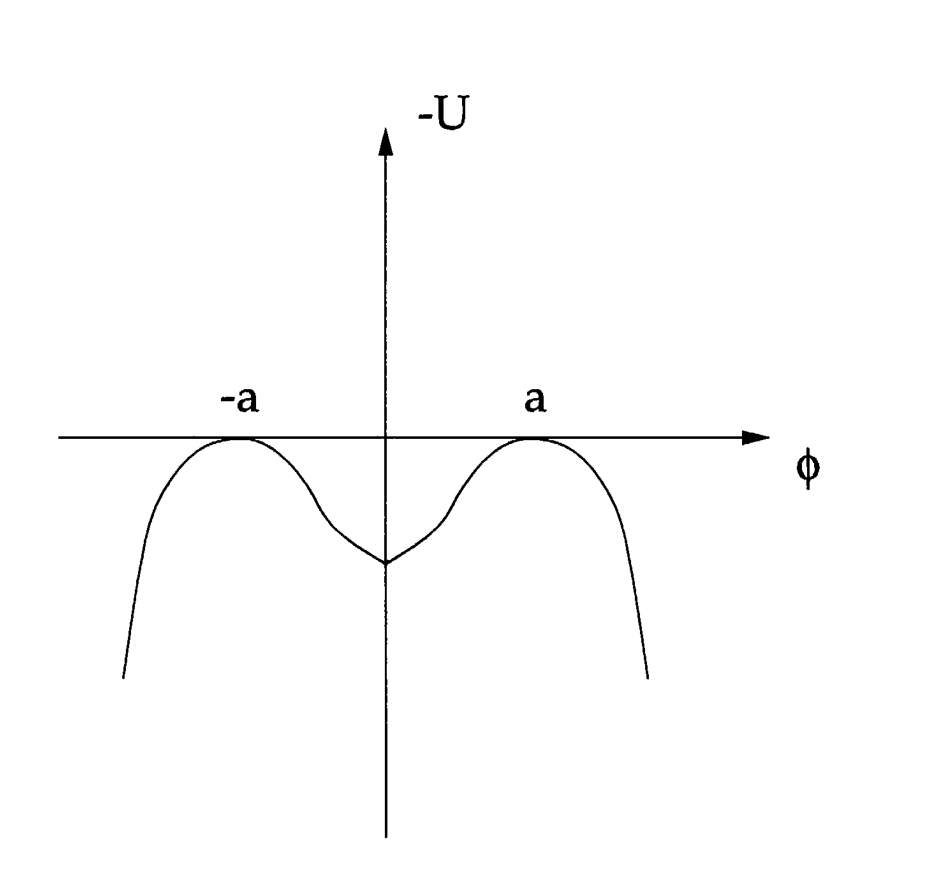
\includegraphics[width=0.5\textwidth]{figs/fig_p011_1.png}
  \caption{「驼峰」形状的势 $-U(x)$：横轴为场 $\phi$，纵轴为 $-U$，两个峰顶位于 $\phi=-a$ 与 $\phi=a$（图中标注 $-a$、$a$），谷底在 $\phi=0$。欧氏路径积分的瞬子解即小球在此势中从一个峰顶滚到另一个峰顶的轨迹。（原文 Figure 1，p.11；原书此图未编号）}
  \label{fig:p11-1}
\end{figure}

\textbf{注 1（Remark 1）.}
函数 $x=\phi_*(\tau)$ 描述一个球在势为 $-U(x)$ 的势场中（如图，形状像驼峰）从一个峰运动到另一个峰。球的初速度取得使从一个峰顶到另一个峰顶所需的时间恰为 $t$。这里把势 $U(x)$ 换成 $-U(x)$ 的理由是：我们做的是欧氏路径积分，也就是说我们做了 Wick 转动 $t\to it$。这个转动把势 $U$ 的 Newton 方程变成势 $-U$ 的 Newton 方程。

\textbf{注 2（Remark 2）.}
当 $t\to\infty$ 时，解 $\phi^*(\tau)$ 有极限；这个极限解在时间平移下唯一。当 $t\to\infty$ 时，解 $\phi^*(\tau)$ 的初速度趋于零。由于在研究 Hamilton 量的低能态时人们关心的是大的 $t$，通常用这个极限解来表达分析，它被称为瞬子（instanton）。

% [Tutor Note: 记号在此处不一致：第 10 页与注 1 用下标星号 $\phi_*(\tau)$、$S_*(t)$，注 2 却写成上标星号 $\phi^*(\tau)$，而下面一句又回到 $S_0=S_*(\infty)$。按上下文二者指同一个极限轨道，译文照原样保留；排版或引用时建议统一为 $\phi_*$，以免与复共轭或「对偶」的常见用法混淆。]

公式 (1.7) 与 $(\psi_+,e^{-Ht/\hbar}\psi_-)$ 为零这一事实矛盾。所以，我们关于存在两个真空的假定是错误的。

\textbf{注（Remark）.}
公式 (1.7) 实际上给出了内积 $(\psi_+,e^{-tH}\psi_-)$ 的正确估计。特别地，$S_0=S_*(\infty)$。这个估计可以用严格的方法加以确认。

在这个论证中，我们从未用到 $\psi_+,\psi_-$ 是实直线上的函数这一事实。我们所使用的只是：它们「定域」在经典平衡态 $a,-a$ 附近，也就是说，对任何局部可观测量 $A$，$A$ 在 $\psi_\pm$ 上的期望值接近相应的经典可观测量在相空间点 $(\pm a,0)$ 处的值。因此，我们的论证与状态空间实现为 $L^2(\mathbb{R})$ 这一选择无关。这使得把这个论证推广到场论的情形变得容易。

考虑时空 $M\times\mathbb{R}$，其中 $M$ 是「空间」。我们将假定已经做了 Wick 转动，使得时空上的度量为 Riemann 乘积度量。我们将假定 $M$ 的体积有限且等于 $V$。

考虑 $M\times\mathbb{R}$ 上带一个标量玻色场 $\phi$ 的场论，它由欧氏 Lagrange 量描述
\begin{equation}
  \tag{1.8}
  \label{eq:1-8}
  \mathcal{L}=\int\left(\frac12(\nabla\phi)^2+U(\phi)\right)dx,
\end{equation}

% 原文 pp.12–20（印刷 pp.1130–1138）
% 第 1 讲第 2 部分：承接第 1 部分（止于公式 (1.8)）；含原文 §1.2 的续论及 §1.3–§1.6 的开头。

% ===== 原文 p.12 =====
其中 $U$ 是前面那个四次势。与以前一样，我们有两个平衡态（equilibrium state）$a$、$-a$。

现在从量子力学的角度考察这个理论。这时可以看出，仍然没有对称性破缺。看清这一点最简单的办法，是先考虑离散的空间 $M$。此时算符代数（operator algebra）是对应于 $M$ 各点的 Heisenberg 代数的有限张量积（tensor product），因此它本身就是一个 Heisenberg 代数；于是我们在量子力学情形用过的表示论（representation theory）论证表明，对称性破缺不会发生。

% [Tutor Note: 「有限张量积仍是 Heisenberg 代数」一句背后的定理是 Stone–von Neumann 唯一性：$M$ 是有限点集，故这里的算符代数只有有限个自由度，其指数化（Weyl 代数）在等价意义下只有唯一的不可约表示，于是任何对称性都可由该表示上的（投影）酉算符实现，Hilbert 空间不会劈成互不相通的部分。作者在 §1.3 指出该论证在无穷体积下失效，原因正在这里：无穷张量积 $\bigotimes_{x\in M}$ 不再有唯一的不可约表示（von Neumann 的无穷张量积理论），不同表示对应不同的「宏观真空」，对称性破缺才成为可能。]

不过，用路径积分（path integral）论证更有启发性。与前面一样，先假设对称性破缺发生。于是我们有两个实现（realization）$\mathcal{H}_+$、$\mathcal{H}_-$，以及两个正交的量子真空 $\Omega_\pm\in\mathcal{H}=\mathcal{H}_+\oplus\mathcal{H}_-$；当 $\hbar$ 很小时，它们在如下意义下「局域化」于平衡点 $a$、$-a$ 附近：
\[
\langle\Omega_\pm,\phi(x_1)\cdots\phi(x_n)\Omega_\pm\rangle\to(\pm a)^n,\qquad \hbar\to0 .
\]

与量子力学的情形一样，内积 $(\Omega_+,e^{-tH/\hbar}\Omega_-)$ 为零。另一方面，用 Feynman–Kac 公式计算它，我们将得到
\begin{equation}
  \tag{1.9}
  \label{eq:1-9}
  (\Omega_+,e^{-tH/\hbar}\Omega_-)\sim e^{-S_*(t)V/\hbar},
\end{equation}
其中 $S_*(t)$ 如前，$V$ 是空间的体积。理由是：最小作用量在空间无关的经典解 $\phi^M_*(\mu,\tau)=\phi_*(\tau)$（$\mu\in M$，$\tau\in\mathbb{R}$）上达到。

% [Tutor Note: (1.9) 的指数里出现体积因子 $V$，这是全段的关键：因为 $M$ 是紧的且作用量是空间积分，最省作用量的构型在空间上必须是常数，于是作用量恰为「单位体积的作用量 $S_*(t)$」乘 $V$。也正因为 $V$ 有限，$e^{-S_*(t)V/\hbar}$ 才非零，才能与「内积为零」矛盾；一旦 $V\to\infty$ 这个矛盾立刻消失——这正是下一节的分水岭。复算时注意 $S_*(t)$ 是 $M$ 为单位体积时的量（与 (1.7) 的定义一致），不要把它再乘一遍体积。]

由于 (1.9) 非零（这里体积 $V$ 有限是本质的），我们得到矛盾。

与量子力学中一样，我们可以定义两组关联函数（correlation function）$W^n_+$、$W^n_-$，它们由在最低能量点 $a$、$-a$ 附近的微扰论计算得到（当然，只有在可重整化的情形，即四维及以下，才能定义它们；此外还应记住，重整化并不是唯一确定的）。我们的论证表明，$W^n_+$、$W^n_-$ 并不是我们的量子理论某个实现的关联函数的小 $\hbar$ 展开。另一方面，函数
\[
W^n_0=\tfrac12\bigl(W^n_++W^n_-\bigr)
\]
则有机会成为实际（非微扰）关联函数的渐近展开。

当 $\dim(M)=1,2$ 时，量子理论 $\mathcal{H}$ 的存在性已在构造性场论（constructive field theory）中建立。在此情形可以证明：（在有限体积下）存在唯一的基态 $\Omega_0$，它是 $G$-不变的；并且该理论关于 $\Omega_0$ 的关联函数确实具有由 $W^n_0$ 给出的渐近展开。

% 原文 §1.3
\subsection{无限体积中量子场论的对称性破缺}

当空间 $M$ 的体积 $V$ 趋于无穷时，上一节的论证失效。表示论论证失效（即使存在紫外截断也失效），因为我们在有限体积情形所用的算符代数的正则表示，现在是对应于各点的空间的无穷张量积；于是我们必须赋予它意义，而可能并不存在 $G$-不变的做法。路径积分论证同样失效。确实，(1.9) 的右端为零，因而对 $(\Omega_+,e^{-tH/\hbar}\Omega_-)$ 的两种计算给出相同答案，我们推不出任何矛盾。此外，若假定我们有一个算符代数的表示 $\mathcal{H}$，其中含两个真空 $\Omega_+$、$\Omega_-$，那么

% ===== 原文 p.13 =====
利用公式
\begin{equation}
  \tag{1.10}
  \label{eq:1-10}
  \langle\Omega_+,\phi(x_1^*)\cdots\phi(x_n^*)\Omega_-\rangle
  =\int_{\substack{\phi:X\to\mathbb{R},\ \phi\to\pm a,\ t\to\pm\infty}}
  \phi(x_1)\cdots\phi(x_n)\,e^{-S(\phi)/\hbar}D\phi,
\end{equation}
（其中对 $x=(\mu,t)$ 有 $x^*=(\mu,it)$），我们推断：对任意的 $x_1,\dots,x_n$，内积 (1.10) 为零。这表明空间 $\mathcal{H}$ 分裂为正交直和
\[
\mathcal{H}=\mathcal{H}_+\oplus\mathcal{H}_-,
\]
其中 $\mathcal{H}_\pm$ 是由真空 $\Omega_+$、$\Omega_-$ 生成的、彼此独立的两个实现的 Hilbert 空间。这意味着对称性破缺可以发生，正如经典理论中那样：量子效应并不必然强到足以恢复对称性。

% [Tutor Note: (1.10) 为何恒为零，作者没有明说，其依据是无穷体积：边界条件 $\phi\to\pm a$（$t\to\pm\infty$）要求场在整个空间上从 $-a$ 过渡到 $+a$，最省作用量的这种构型是一个充满全空间的「畴壁」，其作用量正比于 $V\to\infty$，故右端按 $e^{-\mathrm{const}\cdot V}$ 熄灭。注意这与 (1.9) 恰好相反：那里 $V$ 有限故指数非零，这里 $V=\infty$ 故指数为零。另需留意 $x^*=(\mu,it)$ 表示插入点取在欧氏点上（Wick 转动后的时间），这是把 $\Omega_+$、$\Omega_-$ 之间的矩阵元写成路径积分的必要步骤；$D\phi$ 未写归一化因子，它被 $1=\langle\Omega_\pm,\Omega_\pm\rangle$ 的约定吸收。]

这正是量子场论中实际发生的事。更精确地说，情况如下。

\begin{enumerate}
  \item[(i)] 若对称群 $G$ 是有限群，则从时空维数 2 起，对称性就可以在无穷体积中破缺。例如，在我们考察的那个例子里，对称性破缺确实发生。
  \item[(ii)] 若对称群 $G$ 是连通 Lie 群，则从时空维数 3 起，对称性破缺才可能发生。它在维数 2 不发生，这是一个非凡而极其重要的事实，我们将在 §1.5 讨论。该事实由 S. Coleman 于 1973 年证明（文献见本讲末尾）。
\end{enumerate}

因此，对称性破缺是一种「红外」效应，它与理论在大距离上的行为相联系，并且对时空维数极为敏感。

\textbf{注（Remark）.}
在某种意义下，在维数 2，一旦我们考虑在不同真空之间插值的孤子（soliton），所有真空就都成为一个更统一的故事的一部分。这一点在第 5 讲末尾的一个例子中作了说明；孤子在第九讲中有更系统的讨论。

% 原文 §1.4
\subsection{关联函数的无穷体积渐近}

让我们看看，在有限体积量子场论的无穷体积极限中，对称性是如何破缺的。

考虑从有限体积出发、逼近无穷体积极限的任意一种方式。例如，我们可以把时空取为紧 $d$-流形 $M$，并把 $M$ 的度量 $g$ 放大为 $g\to tg$，其中 $t\to\infty$。在此过程中，$M$ 的任一局部区域都收敛到 $\mathbb{R}^d$。我们考虑在点 $x_i$ 处插入的 $\mathcal{O}_i(x_i)$（其中 $\mathcal{O}_i$ 是任意一组局域算符，不必是基本场），这些点在 $t\to\infty$ 时收敛到 $\mathbb{R}^d$ 中指定的点。\footnote{在我们将于第 19 讲做的、对 Donaldson 理论的一个应用中，除了局域于点的算符之外，还必须考虑与曲面 $\Sigma_\alpha$ 相联系的算符。但那些算符不过是通常局域算符在 $\Sigma_\alpha$ 上的积分；在应用我们即将给出的讨论时，可以把 $\mathcal{O}_i$ 取为这些后者的局域算符。} 然后我们设法分析关联函数
\begin{equation}
  \tag{1.11}
  \label{eq:1-11}
  \langle\mathcal{O}_1(x_1)\cdots\mathcal{O}_n(x_n)\rangle_t
\end{equation}
——即给定乘积在给定 $t$ 值下的关联函数——在大 $t$ 极限下的行为。

另一个本质上是同一件事的例子是：可以把 $M$ 取为 $\mathbb{R}^d$ 中半径为 $t$ 的球，并在球的边界上取某种边界条件。

% ===== 原文 p.14 =====
（更一般地，$M$ 可以是 $\mathbb{R}^d$ 中任意区域，其尺寸被放大 $t$ 倍。）然后人们考虑这样的关联函数：它们通过在服从边界条件的场 $\phi$ 上做路径积分来定义。在此情形下，我们将用符号 (1.11) 来描述在点 $x_i\in\mathbb{R}^d$ 处固定的那些算符的关联函数，这些点在 $t\to\infty$ 时保持不变。

我们首先断言：若乘上一个适当的函数 $C(t)$，则 (1.11) 中的关联函数在 $t\to\infty$ 时具有极限。函数 $C(t)$ 依赖于第一种情形中带度量的 $M$ 的选择细节，或第二种情形中区域的形状与边界条件。一旦关联函数乘上 $C(t)$ 而具有极限，关于该极限我们有如下断言。设 $\langle\mathcal{O}_1(x_1)\cdots\mathcal{O}_n(x_n)\rangle_{(i)}$ 是理论在第 $i$ 个真空中的相应关联函数。则断言是
\begin{equation}
  \tag{1.12}
  \label{eq:1-12}
  \lim_{t\to\infty}C(t)\langle\mathcal{O}_1(x_1)\cdots\mathcal{O}_n(x_n)\rangle_t
  =\sum_i p_i\,\langle\mathcal{O}_1(x_1)\cdots\mathcal{O}_n(x_n)\rangle_{(i)}
\end{equation}
其中 $p_i$ 为某些复数。

直观上，这个重要公式的理由是：当 $t\to\infty$ 时，为了避免作用量过大，空间几乎处处都极其接近某一个真空。但这个充满空间的真空可以是任意一个，即对任意 $i$ 的第 $i$ 个真空。于是关联函数被写成第 $i$ 个真空中关联函数对 $i$ 的求和。不同真空出现不同的常数 $p_i$，是因为函数 $C(t)$ 当 $t\to\infty$ 时的行为，自然只确定到乘一个复常数。没有理由认为对每个 $i$ 都会自然地出现「同一个」常数，所以我们必须用不同的常数去加权不同的真空。（某些 $p_i$ 可以为零，如果在 $t\to\infty$ 极限下某些真空的贡献相比另一些可以忽略。）

在精神上——尽管也许难以严格化——对 (1.12) 的一个有吸引力的解释如下。本理论的关联函数 $\langle\mathcal{O}_1(x_1)\cdots\mathcal{O}_n(x_n)\rangle$ 服从大量由算符乘积展开（OPE）得出的线性关系。由于这些关系是线性的，解空间是一个向量空间。我们有理由希望：这个向量空间的一组基由各真空中的关联函数 $\langle\mathcal{O}_1(x_1)\cdots\mathcal{O}_n(x_n)\rangle_{(i)}$ 给出。(1.12) 的左端定义了此向量空间中的一个元素（因为左端的关联函数当然服从由算符乘积展开得出的一切关系）。所以它必定具有 (1.12) 中所写的那种展开。

% [Tutor Note: 这一段是全节唯一未证明的断言：「OPE 线性关系的解空间由各真空中的关联函数张成」只是一句 "one can reasonably hope"。它的严格化需要两步：其一，用 Osterwalder–Schrader 重构把关联函数翻译成 Hilbert 空间上的真空态与算符代数；其二，证明在 $t\to\infty$ 极限下态空间按「宏观真空」分解（即超选择分块的分解，等价于对 $C^*$ 代数做中心分解）。注意 $p_i$ 是复数而不必是正实数，所以 (1.12) 不是概率式的凸组合；在反射正定的欧氏理论中若取 $C(t)>0$，通常可期望 $p_i\ge0$，但作者有意不作此假设。]

注意，若不止一个 $p_i$ 非零，则由从紧流形 $M$（带或不带边界）出发并取 $t\to\infty$ 得到的关联函数不服从集团分解（cluster decomposition）。除此之外，它们服从场论的所有公理。从公理化的观点看（回忆 [I-Axiomatics] 第 2 讲），人们可以希望证明：服从关联函数的一切公理、只不服从集团分解的函数，可以按 (1.12) 用确实服从集团分解的符号展开。

% [Tutor Note: 指本丛书第 I 卷中的综述 [I-Axiomatics]（公理化场论），其第 2 讲讨论 Wightman 公理与 Osterwalder–Schrader 公理；「除集团分解外满足一切公理」的说法即指：这些函数仍是某个 Hilbert 空间上的真空期望值，只是该空间不是真空唯一的。]

现在我们举出一些可以确定 $p_i$ 的简单情形。若 $M$ 是带平坦度量的环面，则在大多数简单情形下 $p_i$ 相等，因为 $M$ 上的路径积分具有迹的解释，而给定能量的所有态对迹的贡献相同。（在某些条件下可以避免这种相等，例如存在未破缺的离散规范对称性时；但这是我今天不打算讲的内容。）作为另一类例子，设 $M$ 是

% ===== 原文 p.15 =====
$\mathbb{R}^d$ 中的球，并在球面上给定某些边界条件。设我们有一个弱耦合的标量场 $\phi$ 的理论，它具有对称性 $\phi\to-\phi$，以及两个经典基态 $\phi=a$ 与 $-a$。把相应的两个量子真空标为 $+$ 与 $-$。若取边界条件为边界上 $\phi=a$，则当 $t\to\infty$ 时，除了 $+$ 真空之外越来越难看到别的东西，于是 $p_+\neq0$，$p_-=0$。（适当选取 $C(t)$ 可使 $p_+=1$。）反之，若边界上 $\phi=-a$，则 $p_+=0$，$p_-\neq0$。最后，可以取边界上 $\phi=0$。这保持了交换两个真空的那种对称性，故 $p_+=p_-$。

% 原文 §1.5
\subsection{连续对称性破缺}

现在我们来考虑量子场论中的对称性破缺，其中对称群是一个连通 Lie 群。典型的例子是复值玻色场 $\phi$，以及作用量
\begin{equation}
  \tag{1.13}
  \label{eq:1-13}
  \mathcal{L}(\phi)=\int d^dx\left(\frac12|\nabla\phi|^2+\bigl(|\phi|^2-a^2\bigr)^2\right).
\end{equation}

% [Tutor Note: 这里 $\mathcal{L}(\phi)$ 带有 $\int d^dx$，是作用量（action）而非拉氏量密度；本书全篇用 $\mathcal{L}$ 表示作用量，与 §1.6 中「$\mathcal{L}=\mathcal{L}(\phi)$，$X$ 为 Euler–Lagrange 方程的解空间」的用法一致，读文献时不要与通常的 $\mathcal{L}$（密度）混淆。其次，$\nabla$ 必须是 $d$ 维（欧氏）梯度而非仅空间梯度，否则作用量中已含时间积分会使理论失去 Lorentz 不变性。第三，势 $(|\phi|^2-a^2)^2$ 前没有独立的耦合常数，系数取 1 等价于用 $\phi$ 的归一化把耦合固定下来；若要真正做弱耦合展开，须另设小参数（例如把势写成 $\lambda(|\phi|^2-a^2)^2$ 并取 $\lambda\to0$）。]

此作用量具有 $U(1)$ 对称性，作用为 $\phi\to e^{i\theta}\phi$。在经典理论中，最低能量态是 $\phi=ae^{i\theta}$，$\theta\in[0,2\pi)$，所以有对称性破缺。我们将设法弄清量子理论中是否也存在对称性破缺。

上面我们证明了，在一维情形（量子力学）不发生对称性破缺。我们是对实玻色子 $\phi$ 做的；但对复玻色子，论证（用路径积分）甚至更好。例如，对作用量 (1.13)，能量的经典极小点集合是圆 $|\phi|=a$，它是连通的。因此，从一个经典极小点 $ae^{i\theta_1}$ 到另一个 $ae^{i\theta_2}$，不需要翻越势的「驼峰」，而可以沿极小圆走，于是所需作用量比先前更小。因此，上面描述的路径积分计算会表明：在复情形下，态 $\psi_+$、$\psi_-$ 之间的联系比实情形更强。

% [Tutor Note: 这里的 $\psi_\pm$ 是上一部分量子力学双阱讨论中「局域化于 $\pm a$ 附近」的两个态（作者在 (1.7) 之后特别说明：论证只用到它们局域化于经典平衡态，并未用到它们是 $\mathbb{R}$ 上的函数），并非场论中的真空 $\Omega_\pm$。二者的关键差别在指数上：$\psi_\pm$ 之间的隧穿振幅 $\sim e^{-S_0/\hbar}$ 与空间体积无关，故量子力学里隧穿总能恢复对称性；而场论中 $\Omega_\pm$ 之间的矩阵元按 (1.9) 为 $e^{-S_*(t)V/\hbar}$，随 $V\to\infty$ 熄灭，所以场论中隧穿远不足以恢复对称性。连续情形下真正起决定作用的也不是隧穿，而是红外涨落（Coleman 定理；Mermin–Wagner 型论证），这正是下文转向 $\sigma$ 模型与 Goldstone 定理的原因。]

这一效应也许会使我们认为，场论中连续对称性破缺或许不像离散对称性破缺那样容易发生。而确实，结果表明连续对称性破缺在二维不能发生，只能在维数 $\ge3$ 发生。

遗憾的是，这样简单的路径积分论证太粗糙，不足以证明连续对称性破缺在二维不发生。确实，容易看出：在计算 $(\Omega_+,e^{-tH}\Omega_-)$ 的积分中，所有路径在无穷体积下都具有无穷作用量，所以我们推不出任何矛盾。因此，让我们通过考察最简单的例子，来说明为什么对称性在二维得以保持、而在二维以上破缺。

最简单的例子是 $d$ 维自由无质量实标量玻色场理论，它由作用量
\begin{equation}
  \tag{1.14}
  \label{eq:1-14}
  \mathcal{L}_0(\phi)=\int d^dx\left(\frac12(\nabla\phi)^2\right)
\end{equation}
定义。

这个理论具有平移对称性 $\phi\to\phi+c$。让我们证明：该对称性在 $d>2$ 时破缺，在 $d=2$ 时保持。

% ===== 原文 p.16 =====
对 $d>2$，对称性破缺是显然的。确实，在此情形我们有一个由基本场 $\phi$ 生成的 Wightman 场论，它满足 Wightman 公理（[I-Axiomatics] 第 1 讲）。在此理论中，算符 $\phi$ 的单点函数为零，而算符 $\phi+c$ 的单点函数为 $c$。因此变换 $\phi\to\phi+c$ 不保持单点函数。这表明在 $d>2$ 情形下，我们实际上并没有单一的实现，而是有一族实现 $\mathcal{H}_c$，由直线上的点 $c$ 参数化。理论 $\mathcal{H}_c$ 由条件 $\langle\Omega_c,\phi\Omega_c\rangle=c$ 定义，其中 $\Omega_c$ 是 $\mathcal{H}_c$ 的真空。真空 $\Omega_c$「局域化」于经典平衡态 $c$ 附近。映射 $\phi\to\phi+c$ 把 $\mathcal{H}_b$ 变为 $\mathcal{H}_{b+c}$。

% [Tutor Note: 「显然」一词省掉了两点。第一，$\langle\Omega,\phi\Omega\rangle=0$ 的根据是 (1.14) 具有 $\phi\to-\phi$ 的 $\mathbb{Z}_2$ 对称性（作用量只含 $(\nabla\phi)^2$），而 $\phi+c$ 破坏了它；仅凭平移不变性只能断言该单点函数是常数，不能断言它为零。第二，严格说 $\phi+c$ 属于「另一个」理论：Wightman 重构定理保证 $\phi+c$ 仍生成一套满足公理的关联函数，但其真空期望值为 $c\neq0$，故给出与原来不等价的表示 $\mathcal{H}_c$。这两步都依赖 $\phi$ 本身作为算符值分布存在，而这恰是 $d>2$ 才成立的（见下一段 $d=2$ 的反例），所以论证不能平移到二维。]

对 $d=2$，情形不同。问题在于：算符 $\phi$ 在二维没有定义，尽管它的导数有定义。确实，在二维我们有
\begin{equation}
  \tag{1.15}
  \label{eq:1-15}
  \langle\partial\phi(x)\partial\phi(y)\rangle=-\partial_x\partial_y\ln|x-y|,
\end{equation}
于是，如果算符 $\phi$ 以某种方式有定义，我们就会有
\begin{equation}
  \tag{1.16}
  \label{eq:1-16}
  \langle\phi(x)\phi(y)\rangle=-\ln|x-y|+C,
\end{equation}
这与正定性（positivity）矛盾（(1.16) 右端的函数不是正定的）。

% [Tutor Note: (1.15)–(1.16) 与 (1.14) 的归一化相差一个常数：按 $\mathcal{L}_0=\frac12\int d^2x(\nabla\phi)^2$，二维传播子由 $-\Delta G=\delta^{(2)}$ 定出为 $G(x-y)=-\frac{1}{2\pi}\ln|x-y|$，即 (1.16) 右端应带系数 $-\frac{1}{2\pi}$。作者显然取了使系数为 1 的归一化（等价于对 $\phi$ 重新标度并使 $\lambda$ 随之改标）。这不影响「违反正定性」的结论，但下一节 $|x|^{-k^2/\lambda^2}$ 中的指数会因此不带 $2\pi$；读者用标准归一化复算时，应得到 $|x|^{-k^2/(2\pi\lambda^2)}$。至于「违反正定性」：$-\ln|x-y|$ 在 $|x-y|\to\infty$ 时无下界，而正定性要求 $\sum_{i,j}c_ic_j\langle\phi(x_i)\phi(x_j)\rangle\ge0$，取相距很远的两点即可看出矛盾。]

让我们把这一点说得更精确。在二维我们所拥有的，是由从 Schwartz 函数到算符的 Wightman 映射 $\phi$ 生成的量子场论；它并非定义在整个 Schwartz 函数空间 $S(V)$ 上，而只定义在 $V$ 上积分为零的 Schwartz 函数空间 $S_0(V)$ 上。于是 $\phi$ 的导数可以通过
\[
\partial_i\phi(f)=-\phi(\partial_i f)
\]
定义在所有 Schwartz 函数上（右端有意义，因为 $\int\partial_i f=0$）。

然而，在由这样的 $\phi$ 定义的理论中，对称性破缺的问题根本不会出现，因为一开始就没有对称性：在空间 $S_0(V)$ 上，映射 $\phi$ 与 $\phi+c$ 是同一个。所以，为了提出关于对称性破缺的问题，我们应当考虑我们的算符代数的一个扩张，它将具有非平凡的对称性作用。这样做最合理的办法如下。

我们不考察 $\mathbb{R}$ 值无质量标量 $\phi$ 的理论，而考察取值于圆、且作用量相同的场 $\phi$ 的理论。取圆为 $S_\lambda=\mathbb{R}/2\pi\lambda\mathbb{Z}$。作用量与前面相同。在此情形，局域泛函 $\phi$ 没有定义，但我们有局域泛函 $e^{ik\phi/\lambda}$，$k\in\mathbb{Z}$。此理论中的局域泛函是 $e^{i\phi/\lambda}$ 的 Laurent 多项式，其系数是场 $\phi$ 各导数的微分多项式，而不是 $\phi$ 本身的微分多项式。此理论中的平移对称性是 $U(1)$ 对称性：对满足 $|z|=1$ 的复数 $z$，有 $z\circ e^{ik\phi/\lambda}=z^k e^{ik\phi/\lambda}$，而 $z$ 平凡地作用于 $\phi$ 的导数。经典地，此理论有一族真空（平衡态），由 $\phi=c$，$c\in S_\lambda$ 给出。

我们要证明：在这个系统中，对称性在量子力学意义上不破缺。只需证明：对任意形如 $\mathcal{O}=P(\phi)e^{ik\phi/\lambda}$（$k\neq0$）的局域算符 $\mathcal{O}$，单点函数 $\langle\Omega,\mathcal{O}(0)\Omega\rangle$ 为零。\footnote{所有局域算符都是这种形式；并且可以用算符乘积展开证明：若存在一个并非不变的 $n$ 点函数，则存在这样的一个单点函数。} 让我们在

% ===== 原文 p.17 =====
$P=1$ 的情形证明（一般情形的证明类似）。证明：由自由理论中的算符乘积展开（参见 [I-Perturbative QFT] 第 3 讲）我们得到
\[
\langle\Omega,\mathcal{O}(x)\mathcal{O}^*(0)\Omega\rangle=|x|^{-k^2/\lambda^2},
\]
所以这个两点函数在无穷远处趋于零。但由集团性质，该函数在无穷远处的极限是 $|\langle\Omega,\mathcal{O}(0)\Omega\rangle|^2$。故 $\langle\Omega,\mathcal{O}(0)\Omega\rangle=0$。

看对称性不破缺的另一种方式如下。量子化理论的 Hilbert 空间形如
\[
\mathcal{H}=F\otimes F^*\otimes l_2(\mathbb{Z})=\bigoplus_{k\in\mathbb{Z}}(F\otimes F^*)_k,
\]
其中 $F$ 是 Fock 空间。对应于 $\phi$ 的导数的算符保持这个分解，而算符 $e^{ik\phi/\lambda}$ 把空间 $(F\otimes F^*)_{k'}$ 映到空间 $(F\otimes F^*)_{k+k'}$。真空向量 $\Omega$ 属于零分量 $(F\otimes F^*)_0$。这意味着此理论中算符的一切关联函数在 $U(1)$ 作用下不变。特别地，
\[
\langle e^{ik\phi/\lambda}\rangle=\delta_{0k},
\]
这表明真空 $\Omega$ 并不「局域化」于任何经典基态附近，而是均匀地「铺展」在经典基态空间 $S_\lambda$ 上。因此，$U(1)$ 对称性没有破缺。

% [Tutor Note: 这个 Fock 空间分解需要解释：圆值场 $\phi$ 的共轭动量按 $p=k/\lambda$（$k\in\mathbb{Z}$）量子化，故单粒子空间是 $\mathbb{Z}$-分次的；$\mathcal{H}=F\otimes F^*\otimes l_2(\mathbb{Z})$ 中的 $l_2(\mathbb{Z})$ 记录这个动量/绕数扇区，$F\otimes F^*$ 记录左右 mover 的激发。关键在于真空 $\Omega$ 落在 $k=0$ 分量，而 $\phi$ 本身不是良定义的算符（$e^{i\phi/\lambda}$ 才是，它把相邻 $k$ 分量混合），这正是作者前面强调「只有 $e^{ik\phi/\lambda}$ 是局域泛函」的算符代数表述。也正因如此，$\phi\to\phi+c$ 只有在 $c=2\pi\lambda n$ 时才是恒等映射；圆值理论里真正的对称性只剩靶空间的 $U(1)$ 转动，它在 $k\neq0$ 分量上给出相因子 $z^k$，其是否破缺恰由 $\langle e^{ik\phi/\lambda}\rangle=\delta_{0k}$ 判定。]

\textbf{注 1（Remark 1）.} 看一看为什么我们关于 $d>2$ 存在对称性破缺的论证在有限体积下失效，是有启发的；因为我们知道，有限体积下不应有对称性破缺。问题在于：在有限体积下，场 $\phi$ 没有定义，尽管它的导数有定义。确实，由于时空是时间直线与紧空间的乘积，在大距离上它看起来就只是一条直线；$\phi$ 的两点函数（即时空的 Green 函数）在 $|t|$ 大时看起来像一维 Green 函数，即 $-|t|+C+o(1)$。此函数没有下界，因而违反正定性。此外，由考察 $d=2$ 的情形可知，若除一个空间方向外其余方向都被紧化，情形也一样。

\textbf{注 2（Remark 2）.} 上面我们考察了维数 $d>2$ 的自由无质量标量 $\phi$ 的理论，发现其量子真空空间是 $\phi$ 的取值空间（即靶空间 $\mathbb{R}$）。更一般地，若考虑时空为 $\mathbb{R}^d$（$d\ge2$）、靶空间为 $M$（一个黎曼流形）的 $\sigma$ 模型（sigma model），则量子真空空间以及经典基态空间都将是 $M$。（这里你应当暂时忘记，这个非线性 $M$ 的 $\sigma$ 模型是不可重整的。在今天讲座的第 8 部分，我们将把这个 $\sigma$ 模型理解为红外有效理论。）特别地，作为黎曼流形的 $M$ 可以从量子理论中被还原出来，即作为量子真空的模空间（moduli space of vacua）（见下面的注 3）。

另一方面，我们看到对 $d=2$，取值于圆的场 $\phi$ 的理论（它等同于靶空间为 $S_\lambda$ 的二维 $\sigma$ 模型）只有一个真空 $\Omega$。一般二维 $\sigma$ 模型都是这样：其量子真空的模空间通常非常小，与经典基态空间（$=$ 靶空间）不重合。特别地，靶空间不能从量子理论内在地还原出来。例如，圆 $S_\lambda$ 不能从上面考虑的、映入 $S_\lambda$ 的映射的理论中被内在地还原出来。这其实有很好的理由——可以证明，附着于圆 $S_\lambda$ 与 $S_{1/\lambda}$ 的理论是等价的（例如它们的配分函数相同——见 [II-CFT] 第 1 讲）。这正是镜像对称（mirror symmetry）理论的出发点。

% ===== 原文 p.18 =====
\textbf{注 3（Remark 3）.} 考虑一个作用量为
\[
\mathcal{L}=\int d^dx\left(\frac12(\nabla\phi)^2+U(\phi)\right)
\]
的场论，其中 $\phi$ 取值于某个黎曼流形 $M$，$U$ 是 $M$ 上的势函数（$U\ge0$）。设 $M(0)$ 是 $U$ 的零点集。假定 $M(0)$ 非空且光滑，并假定 $U$ 的二阶导数 Hessian 矩阵在 $T_xM/T_xM(0)$ 上、对 $x\in M(0)$ 非退化。设有一个 Lie 群 $G$，它通过等距作用在 $M$ 上、保持 $U$ 不变，且在 $M_0$ 上可迁。在此情形可以证明（在物理的严格性水平上）：由 $\mathcal{L}$ 描述的理论的「红外行为」，与靶空间取为经典真空空间 $M(0)$ 的 $\sigma$ 模型的「红外行为」相同。这一陈述的精确含义在第 1.7 节中解释。（我们可以用截断路径积分来定义这些理论，从而回避不可重整性问题：在截断路径积分中，积分取在步长为 $\Lambda^{-1}$ 的格点上定义的场之上，或取在相对于某个坐标系只有 $|k|<\Lambda$ 的 Fourier 模式的场之上；在这种框架中，截断 $\Lambda$ 不趋于无穷。）这一事实可以启发式地解释：若一个函数 $\phi$ 要具有低能量，它必须缓慢振荡，并且还要靠近极小点轨迹 $M(0)$，即必须接近一个映入 $M(0)$ 的映射。所以低能物理与缓变的、映入 $M(0)$ 的映射有关。

% [Tutor Note: 此处原文作 "acts transitively on $M_0$"，而同段其余各处一律写 $M(0)$（$U$ 的零点集），应视为同一对象的笔误，译文按 $M(0)$ 处理。至于定理本身，作者说 "one can show (at the physical level of rigor)"，其证明思路是：把 $\phi$ 分解为沿 $M(0)$ 的零模（Goldstone 模）与横向的 massive 模，后者质量由 Hessian 的非退化性给出正的下界（这正是「Hessian 在 $T_xM/T_xM(0)$ 上非退化」这一条件的用处），在低能下把 massive 模积分掉只留下 $M(0)$-值映射的 $\sigma$ 模型；$G$ 在 $M(0)$ 上可迁则保证横向质量矩阵在 $M(0)$ 上处处同型。严格的讨论见 [I-Classical Fields] 与后续第 1.7 节；另注意 $U\ge0$ 与 $M(0)\neq\varnothing$ 保证了基态能量为零、真空模空间就是 $M(0)$。]

因此，连续对称性破缺作为红外效应，在由 $\mathcal{L}$ 描述的理论中发生，当且仅当它在相应的 $\sigma$ 模型中发生。于是，由注 2 可知，对称性破缺倾向于不在维数 2 发生，而倾向于在维数 $>2$ 发生。

然而，这些大多只是启发式论证。在下一节，我们将借助 Goldstone 定理，更系统地处理连续对称性破缺问题。

% 原文 §1.6
\subsection{Goldstone 定理}

回忆经典场论中 Noether 定理与守恒流的标准形式。设我们在 $d$ 维时空 $V$ 中有一个作用量 $\mathcal{L}=\mathcal{L}(\phi)$。把相应的 Euler–Lagrange 方程的解空间记为 $X$。

设 $G^s$ 是此作用量的单参数对称群。令
\[
D_\phi:=\left.\frac{d}{ds}\right|_{s=0}G^s\phi .
\]
我们假定 $D_\phi$ 是 $\phi$ 的局域泛函。

设 $\eta\in\Omega^1(X,\Omega^{d-1}(V))$ 是解空间上的典范一形式（canonical one-form），它在 [I-Classical Fields] 与 [I-Homework] 中讨论过（$X$ 上的典范二形式定义为 $\int_C d_X\eta$，其中 $C$ 是 $d-1$ 维闭链）。例如，对无质量标量的自由理论，$\eta$ 的公式为
\begin{equation}
  \tag{1.17}
  \label{eq:1-17}
  \eta(\delta\phi)(x)=\delta\phi(x)*d\phi(x).
\end{equation}

% [Tutor Note: [I-Classical Fields] 与 [I-Homework] 指本丛书第 I 卷中关于经典场论与习题的两部分；$\eta$ 的构造是：在解空间 $X$ 上，场变分 $\delta\phi$ 与 $\phi$ 的时空导数配对，$\eta(\delta\phi)=\delta\phi\,{*}d\phi$ 是把 $\delta\phi$ 与 $*d\phi$（一个 $(d-1)$-形式）相乘得到的 $(d-1)$-形式。这里 $*$ 是时空 $V$ 上的 Hodge 星号，注意它作用在 $d\phi$ 上而非 $\delta\phi$ 上；若把 $*$ 的位置搞错，$J=\eta(D_\phi)$ 会变成一个 $1$-形式而非 $(d-1)$-形式，后面的电荷积分 $\int_C J$（在 $d-1$ 维闭链上）就无法定义。]

设 $J\in\Omega^0(X,\Omega^{d-1}(V))$ 由公式 $J=\eta(D_\phi)$ 定义。由于 $D_\phi$ 是局域的，$J$ 也是局域的。于是 $J$ 是 $X$ 上取值于 $\Omega^{d-1}(V)$ 的局域泛函。例如，若 $\mathcal{L}$ 是无质量标量自由理论的作用量，且 $G^s\phi=\phi+s$，则 $D_\phi=1$，故 $J(x)=*d\phi(x)$。局域泛函 $J$ 称为对应于对称性 $G^s$ 的流（current）。流的主要性质是它守恒，即 $d_V J=0$。这由 $d_V\eta=0$ 这一事实推出。

% [Tutor Note: 原文此句印作 "This follows form the fact that $d_V\eta=0$"，"form" 系 "from" 之误（p.1136 末行）。另注意此处「守恒」是外微分意义下的 $d_VJ=0$，等价于 $\partial_\mu J^\mu=0$；而 $J$ 是 $(d-1)$-形式而非矢量，二者通过 Hodge 星号对应，做分量计算时别忘了 $J^\mu=(\ast J)$ 的指标位置。]

% ===== 原文 p.19 =====
在有限体积下，定义电荷泛函（charge functional）$Q=\int_C J(x)$ 是有用的，其中 $C$ 是某个类空闭链（例如 $t=\text{const}$）。由于流守恒，只要 $C$ 代表「空间」的基本同调类，这个量就与闭链的选取无关。若 $\Omega=\int_C d_X\eta$ 是 $X$ 上的非退化二形式，则 $Q$ 是定义对称群 $G^s$ 的 Hamiltonian，其意义是
\[
\left.\frac{d}{ds}\right|_{s=0}(G^s)^*F=\{F,Q\},
\]
其中 $\{\,,\}$ 是 $S$ 上的 Poisson 括号，$F$ 是 $X$ 上任一局域泛函。

在无穷体积下，泛函 $Q$ 不一定有定义，因为积分不收敛。此时方便的做法是选取时间坐标 $t$，令 $C=C_0=\{t=0\}$ 为初值面，然后定义「截断电荷泛函」
\begin{equation}
  \tag{1.18}
  \label{eq:1-18}
  Q_f=\int_{C_0}f(x)J(x),
\end{equation}
其中 $f:C_0\to\mathbb{R}$ 是 Schwartz 函数。此时极限 $\lim_{f\to1}Q_f$ 不存在，但对任一局域泛函 $F$ 有
\begin{equation}
  \tag{1.19}
  \label{eq:1-19}
  \lim_{f\to1}\{F,Q_f\}=\left.\frac{d}{ds}\right|_{s=0}(G^s)^*F.
\end{equation}

\textbf{注（Remark）.} 所谓 $f\to1$，是指 $f$ 在任一紧集上一致收敛到 1，且 $f$ 的所有导数在整个空间上一致趋于零。

在量子理论中，故事相同，只是（局域）泛函被换为局域算符，Poisson 括号被换为对易子乘以 $i$。也就是说，对任一单参数对称性 $G^s$，存在取值于 $(d-1)$-形式的局域算符 $J(x)$，它守恒；并且电荷算符 $Q=\int_C J(x)$（在有限体积下）具有性质
\begin{equation}
  \tag{1.20}
  \label{eq:1-20}
  [F,Q]=-i\left.\frac{d}{ds}\right|_{s=0}(G^s)^*F.
\end{equation}

% [Tutor Note: (1.19) 与 (1.20) 之间相差因子 $-i$，这对应 Dirac 量子化规则 $\{\,,\}\to\frac1i[\,,\ ]$；但符号要小心：若按 (1.19) 定义 $\{F,Q\}\equiv D$（$D=\frac{d}{ds}|_{s=0}(G^s)^*F$），标准规则给出的是 $[F,Q]=iD$，而 (1.20) 写的是 $-iD$。二者之差等价于把生成元取为 $G^s=e^{-isQ}$ 而不是 $e^{isQ}$，也就是 $\eta$（从而 $J$）的整体定向约定。由于后文只用到 $[Q_f,\phi]$，(1.21) 中这个整体符号无关紧要；但读者若拿 (1.20) 与教科书中 $[Q,\phi]=-i\,\delta\phi$ 的写法对照，务必先统一 $Q$ 的符号约定，否则会误以为 (1.19)–(1.20) 自相矛盾。另注意 $\lim_{f\to1}Q_f$ 不存在而 $\lim_{f\to1}\{F,Q_f\}$ 存在，原因是对易子把积分限制在 $F$ 的支集附近，这正是「无穷体积下电荷算符不是算符、但其导数是」的标准图像。最后，作者说「$\{\,,\}$ 是 $S$ 上的 Poisson 括号」，而全篇解空间记作 $X$，此处 $S$ 疑为 $X$ 之误（或指前文引入的相空间），译文保留原符号 $S$。]

无穷体积的情形与经典理论中同样处理，即考虑截断算符 $Q_f$。

现在我们来讨论 Goldstone 定理。设由 $\mathcal{L}$ 定义的理论中的对称性 $G^s$ 不仅在经典上破缺，而且在量子力学意义上也破缺。在此情形，若我们有理论的一个解 $\mathcal{H}$（一个带有算符代数作用的 Hilbert 空间），则存在一个标量局域算符 $\phi$，其单点函数在对称变换下并非不变。

\textbf{注（Remark）.} 严格说来，我们只知道某个 $n$ 点函数并非不变；但在一切已知的对称性破缺情形中，也存在一个并非不变的单点函数。（利用算符乘积展开可以论证：若存在一个并非不变的 $n$ 点函数，则存在一个并非不变的单点函数。）

设 $Q_f$ 是对称性 $G^s$ 的截断电荷算符。我们有
\begin{equation}
  \tag{1.21}
  \label{eq:1-21}
  \langle\Omega|[Q_f,\phi(0)]|\Omega\rangle\neq0,
\end{equation}
其中 $f$ 充分接近 1。于是对某个 $x$ 有 $\langle\Omega|[J(x),\phi(0)]|\Omega\rangle\neq0$。

% ===== 原文 p.20 =====
考虑两点函数
\begin{equation}
  \tag{1.22}
  \label{eq:1-22}
  M_+(x):=\langle\Omega|J(x)\phi(0)|\Omega\rangle,\qquad
  M_-(x):=\langle\Omega|\phi(0)J(x)|\Omega\rangle
\end{equation}
（它们是 $V$ 上的 $(d-1)$ 形式）。由于对称性破缺，$M_+\neq M_-$；不过由类空间隔，当 $x$ 类空时二者重合。

设 $\mathcal{H}=\int_{p\in V_+}\mathcal{H}_p$ 是 $\mathcal{H}$ 关于平移群作用的谱分解（这里 $V_+$ 是整个光锥的正向部分）。利用内积对中间态（intermediate state）的分解
\[
\begin{aligned}
\langle J(x)\Omega,\phi(0)\Omega\rangle
&=\sum_n\langle J(x)\Omega,n\rangle\langle n,\phi(0)\Omega\rangle,
\end{aligned}
\]
我们得到
\begin{equation}
  \tag{1.23}
  \label{eq:1-23}
  M_\pm(x)=\int_{V_+}K_\pm(x,p)\,dp,
\end{equation}
其中 $K_+(x,p)$、$K_-(x,p)$ 是四动量为 $p$ 的中间态对 $M_+$、$M_-$ 的贡献（$K_\pm$ 是 $p$ 的向量值分布）。

由于 Lorentz 不变性，分布 $K_+$、$K_-$ 形如
\begin{equation}
  \tag{1.24}
  \label{eq:1-24}
  K_\pm=p\,e^{\pm ipx}\rho_\pm(-p^2),
\end{equation}
其中 $\rho_\pm(s)$ 是半直线 $s\ge0$ 上的分布。

% [Tutor Note: 这条论证里有两个容易混淆的输入，作者只用一句话带过。第一，「$M(x)$ 对类空的 $x$ 为零」用的是局域算符在类空间隔上的对易性（因果性）：$[J(x),\phi(0)]=0$（$x$ 类空），故 $M_+=M_-$。第二，「$W_m(x)=W_m(-x)$（$x$ 类空）」用的是 Klein–Gordon 传播子对 $x\to-x$ 的偶性。两者是不同的性质，缺一不可：前者给 $M_+-M_-$ 的类空消失，后者才使 (1.26) 中的 $\rho_+-\rho_-$ 能进一步化为 (1.27) 的形式。复算时若把 $x\to-x$ 的偶性误用到类时区（那里 $W_m(x)\neq W_m(-x)$，差一个 $2i\,\mathrm{Im}$ 项），就会错失 (1.28) 的推论。]

% [Tutor Note: (1.24) 把指标「藏」起来了：$J$ 是 $(d-1)$ 形式，故 $K_\pm$ 实际带有矢量指标，准确写法是 $K_\pm{}^\mu(x,p)=p^\mu e^{\pm ipx}\rho_\pm(-p^2)$。Lorentz 不变性只允许 $K^\mu$ 正比于唯一可用的四维向量 $p^\mu$（其余标量因子只能是 $p^2$ 的函数），而之所以写成 $\rho_\pm(-p^2)$ 而非 $\rho_\pm(p^2)$：本讲采用 $(-,+,+,+)$ 号差（由 (1.25) 下方的 $p^2=-m^2$ 与类空的 $x^2>0$ 可见），质量壳上 $-p^2=m^2\ge0$，这样宗量才落在半直线 $s\ge0$ 上，与「$\rho_\pm(s)$ 定义在 $s\ge0$」相符。若把 $p^\mu$ 写成 $p_\mu$，或漏掉 $e^{\pm ipx}$ 中与 $\rho_\pm$ 相应的 $\pm$，(1.25) 里 $W_m(\pm x)$ 的 $\pm$ 就会配错。]

由此得到
\begin{equation}
  \tag{1.25}
  \label{eq:1-25}
  M_\pm(x)=i*d_V\int_0^\infty\rho_\pm(m^2)W_m(\pm x)\,dm^2,
\end{equation}
其中 $W_m(x)=\int_{\mathcal{O}^+_m}e^{ipx}dp$ 是 [I-Perturbative QFT] 第 1 讲中定义的、质量为 $m$ 的 Klein–Gordon 传播子（$\mathcal{O}^+_m$ 是双曲面 $p^2=-m^2$ 的上叶）。

令 $M(x)=M_+(x)-M_-(x)$。由于当 $x$ 类空时 $W_m(x)=W_m(-x)$，对类空的 $x$，(1.25) 给出
\begin{equation}
  \tag{1.26}
  \label{eq:1-26}
  M(x)=i*d_V\int_0^\infty\bigl(\rho_+(m^2)-\rho_-(m^2)\bigr)W_m(x)\,dm^2.
\end{equation}

然而，正如我们已经提到的，由类空间隔，$M(x)$ 对类空的 $x$ 为零。这意味着 $\rho_+=\rho_-=\rho$，于是 (1.25) 给出
\begin{equation}
  \tag{1.27}
  \label{eq:1-27}
  M(x)=i*d_V\int_0^\infty\rho(m^2)\bigl(W_m(x)-W_m(-x)\bigr)dm^2.
\end{equation}

在满足 $x^2>0$ 的点 $x$ 处对 (1.27) 两端求导，并利用流的守恒与 Klein–Gordon 方程 $\nabla^2W_m=-m^2W_m$，我们得到
\begin{equation}
  \tag{1.28}
  \label{eq:1-28}
  \int_0^\infty m^2\rho(m^2)\bigl(W_m(x)-W_m(-x)\bigr)dm^2=0.
\end{equation}

取 Fourier 变换，我们得到
\begin{equation}
  \tag{1.29}
  \label{eq:1-29}
  p^2\rho(-p^2)=0.
\end{equation}

% [Tutor Note: 从 (1.27) 到 (1.28) 的「differentiating both sides」跳过了三步：先对 (1.27) 取外微分，用流守恒 $d_VJ=0$（即 $\partial_\mu M^\mu=0$）把微分从 $d_V$ 转移到 $W_m$ 上；再用 Klein–Gordon 方程把 $W_m$ 的二阶导数换成 $-m^2W_m$，于是 $m^2$ 作为本征值被「提」到积分号内（这就是被积函数多出因子 $m^2$ 的来源）；最后约去公共的 $i$ 与 $d_V$。这里还有一个符号陷阱：作者在 (1.25) 下方写 $p^2=-m^2$、在本页写类空的 $x^2>0$，说明号差是 $(-,+,+,+)$；在该号差下 $\partial_\mu\partial^\mu e^{ipx}=-p^2e^{ipx}=m^2e^{ipx}$，故与 (1.28) 相容的写法应是 $\nabla^2W_m=+m^2W_m$，即他把 $\nabla^2$ 定义为 $-\partial_\mu\partial^\mu$。由于 (1.28) 右端为零，这个整体符号不影响结论。而 (1.29) 说明 $\rho$ 的支撑集在 $p^2=0$：$\langle\Omega|[J(x),\phi(0)]|\Omega\rangle\neq0$ 只能由无质量中间态贡献，这个无质量粒子即 Goldstone 玻色子（此即 Goldstone 定理的谱表述）。]

% 原文 pp.21–28（印刷 pp.1139–1146）
% 第 1 讲（Lecture 1: Symmetry Breaking）第 3 部分：Goldstone 定理的证明与推论、
% 纯不可重整场论的红外行为（§1.7）、Goldstone 玻色子的有效作用量（§1.8）、参考文献

% ===== 原文 p.21 =====
于是 $\rho(m^2)=c\delta(m^2)$，其中 $c$ 是常数。常数 $c$ 不能为零，否则我们就会证明 $[J(x),\phi(0)]$ 在真空中的期望值为零，而这与对称性破缺的假设相矛盾。

这一论证表明，两点函数 $\langle\Omega,J(x)\phi(0)\Omega\rangle$ 的全部贡献都来自零质量的中间态。这意味着 $L^2(\mathcal{O}_0^+)$ 含于 $\mathcal{H}$ 的离散谱之中（即作为 Poincaré 群的一个真正的子表示（subrepresentation））。在场论中，这样的子表示被解释为一个自旋为零的无质量粒子。于是我们证明了下述命题，它就以 Goldstone 定理之名著称：

\noindent\textbf{定理}。\emph{在连续对称性破缺的场论实现所处的 Hilbert 空间 $\mathcal{H}$ 中，存在一个无质量标量（即 Poincaré 群的一个与 $L^2(\mathcal{O}_0^+)$ 同构的子表示），它由破缺对称性的流所产生。}

\noindent\textbf{注（Remark）}。「产生（created）」的意思是 $J(x)\Omega$ 与该子表示不正交。

\noindent\textbf{定义}。我们找到的这个无质量标量称为与破缺对称性 $G^s$ 相对应的 Goldstone 玻色子（Goldstone boson）。

\noindent\textbf{注 1}。若关于 $G^s$ 的对称性未被破缺，则 $\lim_{f\to1}Q_f\Omega$ 将为零。另一方面，当对称性破缺发生时，$Q_f$ 会从真空中产生 Goldstone 玻色子。因此，Goldstone 玻色子「度量」了对称性的失效。

\noindent\textbf{注 2}。Goldstone 玻色子不仅可由对称性的流算符产生，也可由其他局域算符产生。事实上，正如我们在 Goldstone 定理的证明中所见，任何一个标量局域算符，只要其单点函数在该对称性下不是不变的，它就会产生 Goldstone 玻色子。

\noindent\textbf{注 3}。Goldstone 定理并未断言 Goldstone 玻色子是自由的，即并未断言它可以由一个自由场 $\phi(x)$ 产生。事实上，正如我们将看到的，情况往往并非如此。

\noindent\textbf{注 4}。如果连续对称性破缺在经典层面就已发生，那么 Goldstone 玻色子在微扰论中已经可以看到。作为例子，考虑拉氏量 (1.13)。考虑经典基态 $\phi=a$。这个态是简并的。因此，如果我们引入实变量 $\phi_1=\operatorname{Re}\phi-a$，$\phi_2=\operatorname{Im}\phi$，并用这些变量改写拉氏量，那么由于极小值的简并性，场 $\phi_2$ 在经典上将是零质量的。因此，如果我们计算 $\phi_2$ 的两点函数，它将在 $k^2=0$ 处有一个极点（模掉微扰参数）。当然，在缺乏对称性的情况下，圈项可能移动这个极点。换句话说，经典上无质量的 $\phi_2$ 在量子层面可能获得非零质量。Goldstone 定理告诉我们的是：如果存在一个自发破缺的对称性，使得条件 $\phi_2=0$ 在该对称性下不是不变的，那么上述情形就不会发生。

% [Tutor Note: 注 4 中的「模掉微扰参数」有多层含义，易被读漏：其一，经典上 $\phi_2$ 的质量严格为零，是因为势沿 $U(1)$ 的轨道方向（即 $\phi_2$ 方向）是平坦的，二阶导数 $\partial^2V/\partial\phi_2^2|_{a}=0$ 是简并极小值的直接推论；其二，一旦计入圈图，$\phi_2$ 的自能会得到 $\mathcal{O}(\lambda)$ 的修正，从而把传播子的极点从 $k^2=0$ 移到 $k^2=\mathcal{O}(\lambda a^2)$；其三，作者说「若存在使 $\phi_2=0$ 不变性被破坏的自发破缺对称性，则极点仍钉在 $k^2=0$」，其实质是 Ward 恒等式（流守恒）把自能的极点位置与破缺生成元的单点函数绑定在一起。另须注意：本条只对 $d\ge3$ 成立；在 $d=2$ 时由本页推论，$\phi_2$ 不可能真正无质量（Coleman 定理），此时上面的微扰论证在红外区失效。]

\noindent\textbf{推论}。连续对称性破缺不会发生在 2 维中。

\noindent\textbf{证明}。否则，由 Goldstone 定理，Goldstone 玻色子就必须存在。但在二维量子场论中，不可能存在由局域算符产生的无质量粒子。的确，该算符在动量空间中的两点函数等于 $w(k^2)=\int_0^\infty\frac{d\mu(m^2)}{k^2+m^2}$，其中 $\mu$ 是谱测度（spectral measure）。如果

% ===== 原文 p.22 =====
存在无质量粒子，则该测度在 $m=0$ 处将有一个原子（atom，即 $\delta$ 型点质量）。但在此情形下，位置空间中的两点函数 $W(x)$ 在无穷远处将表现为 $-C\ln x^2$，也就是违反正性公理（positivity axiom）。$\square$

% [Tutor Note: 这里的「原子」是测度论的术语，指谱测度在 $m=0$ 处的点质量 $c\,\delta(m^2)$，而非物理上的原子；它正是上一页 $\rho(m^2)=c\delta(m^2)$ 中 $c\neq0$ 的另一种说法。$2$ 维无质量标量的 Wightman 函数在 Minkowski 号差下为 $\sim-\frac{1}{4\pi}\ln(-x^2+i0)$（Euclidean 中为 $-\frac{1}{2\pi}\ln|x|$），其对数的增长意味着它可以任意缓慢地发散，从而使某些检验函数的 smearing 给出负的「模方」，破坏 Hilbert 空间的正定性；系数的符号由 $|c|^2>0$ 固定，不能靠重新定义 $c$ 来翻转。严格的证明即 Coleman 定理（S. Coleman, Comm. Math. Phys. \textbf{31} (1973) 259），其论证依赖红外行为，与 $d\ge3$ 的情形有本质区别——高维时 $\ln$ 换成 $1/x^{(d-2)}$，衰减足够快，正性不受威胁。]

现在假设我们有一个具有李群 $G$ 对称性的拉氏量。假设 $\mathcal{H}$ 是由该拉氏量定义的量子场论的一个实现，其稳定化子（stabilizer）为 $H\subset G$。此时人们说：在实现 $\mathcal{H}$ 中，$G$ 对称性被自发破缺（spontaneously broken）到 $H$。（由上述推论，时空维数必然大于二。）

设 $\mathfrak{g},\mathfrak{h}$ 分别为 $G,H$ 的李代数。Goldstone 定理蕴涵

\noindent\textbf{推论}。$\mathcal{H}$ 的离散谱中含有一个与 $L^2(\mathcal{O}_0^+)\otimes(\mathfrak{g}/\mathfrak{h})$ 同构的子表示。

\noindent\textbf{证明}。证明是显然的：若非如此，则存在元素 $Y\in\mathfrak{g}$、$Y\notin\mathfrak{h}$，使得当 $f\to1$ 时 $Q_Y^f\Omega\to0$（弱收敛）。这意味着关于 $Y$ 的对称性未被破缺——矛盾。

% [Tutor Note: 「证明是显然的」省略了两步。第一步是：若 $Q_Y^f\Omega\to0$（弱），则由 $\Omega$ 在 $\mathcal{H}$ 上的循环性（cyclicity）可推出 $[Q_Y^f,A]\Omega\to0$ 对稠密多个局域算符 $A$ 成立，故 $Y$ 生成的单参数群在真空上平凡作用，即 $Y\in\mathfrak{h}$——这与 $Y\notin\mathfrak{h}$ 矛盾；这里用到 $\Omega$ 是分离态（separating），即 $A\Omega=0\Rightarrow A=0$。第二步是张量因子：$L^2(\mathcal{O}_0^+)\otimes(\mathfrak{g}/\mathfrak{h})$ 中 $\mathfrak{g}/\mathfrak{h}$ 是平凡表示，只贡献重数，故 Goldstone 玻色子的个数为 $\dim(\mathfrak{g}/\mathfrak{h})=\dim G-\dim H$（对紧致 $G$、闭子群 $H$）。注意商空间 $\mathfrak{g}/\mathfrak{h}$ 只在选定真空（即选定 $H$）后才有意义，换一个真空相当于把 $\mathfrak{h}$ 共轭化，重数不变但具体哪些生成元「破缺」会变。附带指出：原文 "if this is not so than there exists" 中的 than 应为 then，系原书排印笔误。]

该推论意味着：对应于线性无关的破缺无穷小对称性的 Goldstone 玻色子也是线性无关的。

\noindent\textbf{例}。设 $\phi:\mathbb{R}^d\to\mathbb{R}^N$ 是标量场，并考虑拉氏量

\begin{equation}
  \tag{1.30}
  \label{eq:1-30}
  \mathcal{L}(\phi)=\int d^dx\left(\frac12(\nabla\phi)^2+\frac{g}{4!}(\phi^2-a^2)^2\right).
\end{equation}

这个拉氏量具有 $SO(N)$ 对称性，其经典基态空间是 $S^{N-1}$。因此，经典上 $SO(N)$ 对称性被破缺到 $SO(N-1)$。如我们所知，若 $d>2$，同样的情形在量子层面也会发生（对于弱耦合理论），于是该理论的任何实现（解）都有 $N-1$ 个独立的 Goldstone 玻色子。

设 $P$ 是坐标为 $(0,0,\dots,0,a)$ 的经典极小点。考虑该理论的实现 $\mathcal{H}_P$，其中真空 $\Omega$ 局域化在 $P$ 附近。设 $Y_i\in\mathfrak{so}_N$，$i=1,\dots,N-1$，是 $\mathbb{R}^N$ 的基向量 $e_i,e_N$ 所生成的平面内的无穷小转动。算符 $\phi_i$ 的单点函数在 $Y_i$ 下不是不变的，因此 $\phi_i$ 产生对应于 $Y_i$ 的 Goldstone 玻色子。

我们可以构造低能（非真空）态，它们并非仅仅局域化在单个经典基态 $P$ 附近。的确，设 $P'$ 是另一个经典基态，并设 $Y\in\mathfrak{so}(N)$ 是使 $e^YP=P'$ 的元素。设 $J_Y$ 是对应于 $Y$ 的流，$Q_Y^f$ 是相应的截断电荷（cutoff charge）。则态 $e^{iQ_Y^f}\Omega$ 是一个局域化在 $P'$ 附近的低能态。

在长距离上，该理论的行为将如同一个映入经典基态空间的 $\sigma$ 模型。对 $N\ge3$ 这是一个有趣的论断，因为此时靶空间（$S^{N-1}$）不是平坦的，所以该 $\sigma$ 模型不是自由的。更确切地说，在低能（或长距离）下，玻色子 $\phi_i$（$i=1,\dots,N-1$）的理论在第零阶近似（即只考虑散射振幅的零动量极限）中是自由的，但在第一阶近似（即考虑小动量下的一阶非零项）中它将不再自由，而由映入球面的 $\sigma$ 模型的拉氏量描述。

% [Tutor Note: 此处 $Y_i$ 的选取有指标上的陷阱：$Y_i$ 是平面 $(e_i,e_N)$ 内的转动生成元，它把 $\phi_i$ 与 $\phi_N$ 混合，即 $\delta\phi_i\propto\phi_N$、$\delta\phi_N\propto-\phi_i$。在真空附近 $\phi_N\simeq a\neq0$ 而 $\langle\phi_i\rangle=0$，故 $\langle\delta\phi_i\rangle\propto a$ 不为零，$\phi_i$ 的单点函数确实破缺；反之若误取平面 $(e_i,e_j)$（$i,j<N$）内的转动，则 $\langle\delta\phi_i\rangle=0$，单点函数不变，那里的生成元属于 $\mathfrak{h}$，不产生 Goldstone 玻色子。这正好印证上一条推论：可用的破缺生成元恰为 $\dim(\mathfrak{so}_N/\mathfrak{so}_{N-1})=N-1$ 个。]

% ===== 原文 p.23 =====
\subsection{纯不可重整场论的红外行为}
% 原文 §1.7：Infrared behavior of purely non-renormalizable field theories

在本节中，我们将澄清下述论断的含义与依据：对于 $d>2$，一个所有无质量粒子都是 Goldstone 玻色子的量子场论，在红外极限下的行为如同一个映入真空态空间的 $\sigma$ 模型。

假设我们有一个由拉氏量 $\mathcal{L}$ 描述的纯不可重整（purely nonrenormalizable）场论。若一个拉氏量的所有耦合都具有负的标度维数，我们就称它为纯不可重整的。这类拉氏量的一个例子是 $d>2$ 的 $\sigma$ 模型的拉氏量。这样的拉氏量不适合在 UV 极限下做微扰重整化，但在 IR 极限下不造成任何问题，因为从 Wilson 重整化群流的观点看，它们的所有相互作用都是 IR 无关（irrelevant）的。也就是说，如果我们引入一个 UV 动量截断 $\Lambda$（此时并不将它送到无穷），就可以微扰地定义 $\mathcal{L}$ 的关联函数：关联函数是所有费曼图振幅之和，这些图按通常方式计算，积分在 $|q|<\Lambda$ 处截断。由于 $\mathcal{L}$ 没有质量项，可能存在一些 IR 发散，但当所有耦合都具有负维数时，它们是相当温和的；它们的含义只是：$S$ 矩阵在零动量附近的动量中不是解析的。（我们稍后会给出一个例子；参看本讲末尾的那张图。）

现在假设我们想计算动量表象中 $n$ 点函数在点 $k_i=0$ 附近的渐近展开。我们将有（其中 $\sum k_i=0$）：

\begin{equation}
  \tag{1.31}
  \label{eq:1-31}
  G_n(k_1,\dots,k_n)=\frac{G_n^0(k_1,\dots,k_n)}{k_1^2\cdots k_n^2},
\end{equation}

其中，按照我们在 Kazhdan 的讲演中学到的 LSZ 约化公式，$G_n^0$ 是 $n$ 个 Goldstone 玻色子散射的 $S$ 矩阵元。$G_n^0$ 在 $k_i=0$ 附近不是解析的，因此我们不能把它展开成幂级数；但我们可以考察它在整体标度变换 $k_i\to\lambda k_i$ 下的行为。

这个级数的关键性质（它来自纯不可重整性）是：模掉按 $\lambda$ 的任意给定幂次标度的项，$G_n^0$ 由有限多个费曼图决定。换句话说，纯不可重整性加上量纲分析蕴涵：越来越高阶的项按 $\lambda$ 的越来越高次幂标度。因此，我们只须借助微扰论中有限多项，就能得到关联函数在 $k_i$ 中任意阶的 IR 渐近行为。

% [Tutor Note: (1.31) 只是把「去掉外腿传播子」这一步写成了公式，切勿把 $G_n^0$ 与 $n$ 点 Green 函数 $G_n$ 混为一谈：$G_n$ 在每个 $k_i^2\to0$ 处有极点（极点留数即 $S$ 矩阵元），故 $G_n$ 本身根本没有 $k_i\to0$ 的幂级数展开，只有去掉极点因子后的 $G_n^0$ 才有。所谓「按 $\lambda$ 的幂次标度」，指的是在 $k_i\to\lambda k_i$ 下令 $\lambda\to0$：$G_n^0$ 的展开中第 $m$ 阶项恰含 $2m$ 个导数，故按 $\lambda^{2m}$ 标度（等价地，每个额外导数贡献一个 $\lambda$ 的幂）。若自行推导，注意 $n$ 个外腿的极点因子共给出 $\lambda^{2n}$，并且不同作者对外腿的归一化（是否提出整体常数、是否用 $\mathrm{i}$ 因子）约定不同，比较结果前须先核对这一点。]

在纯不可重整理论中构造的圈图当然也有紫外发散。我们把该纯不可重整理论视为低能有效场论，从这个观点看，我们只是以任意方式正规化这些发散，并把低能有效拉氏量中所有可能项的系数当作唯象参数。模掉 $\lambda$ 的任意幂次，只有有限多个这样的项是相关（relevant）的（因为当 $d>2$ 时，只有有限多个维数低于某个给定常数的算符）。

现在假设我们有一个真正的量子场论，由某个可重整拉氏量 $\mathcal{L}'$ 给出。当我们说由 $\mathcal{L}'$ 定义的理论在 IR 极限下、在给定精度内由（同一组场上的）纯不可重整拉氏量 $\mathcal{L}$ 描述时，我们的意思是：模掉在 $k_i\to\lambda k_i$ 下按 $\lambda$ 的给定幂次标度的项，由 (1.31) 给出的函数 $G_n^0$ 对 $\mathcal{L}$ 与对 $\mathcal{L}'$ 是相同的。

% ===== 原文 p.24 =====
例如，当我们在上一节末尾说，在低能（或长距离）下，玻色子 $\phi_i$（$i=1,\dots,N-1$）的理论在第零阶近似中是自由的，而在第一阶近似中由坐标为 $\phi_i$ 的球面上的 $\sigma$ 模型的拉氏量描述时，我们的意思是：$\phi_i$ 的函数 $G_n^0(k_1,\dots,k_n)$ 与自由理论中的相同（模 $o(1)$），并与 $\sigma$ 模型中的相同（模 $o(k^2)$）。

计算 $k$ 展开的更高阶项，人们可以构造一个纯不可重整的低能有效理论，它将在红外区以任意所需的精度描述我们的理论。

\noindent\textbf{注}。由于函数 $G_n^0(k_1,\dots,k_n)$ 到轨迹（locus）$k_i^2=0$（其中 $k_i$ 不必为零）上的限制就是 $S$ 矩阵元，该断言的意思是：在 $k^0$ 阶，模型 (1.30) 中 $n$ 个 Goldstone 玻色子的散射矩阵与自由理论中一样为零；而 $k^2$ 阶的项由真空态空间的曲率决定，特别地当 $N>2$ 时不为零。

\subsection{Goldstone 玻色子的有效作用量}
% 原文 §1.8：Effective action for Goldstone bosons

让我们落实上一节的一般讨论，并在一个具体例子中算出 Goldstone 玻色子的有效作用量（effective action）。考虑一个把 $SO(3)$ 破缺到 $SO(2)=U(1)$ 的理论。我们有三个实标量，它们可以组合成一个三分量对象 $\vec\phi$，在 $SO(3)$ 的三维表示中变换。拉氏量为

\[
  \mathcal{L}=\frac1\lambda\int d^nx\left[\frac12(\partial_\mu\vec\phi)^2+V(|\vec\phi|)\right],
\]

其中，令 $\rho=|\vec\phi|$，$V(\rho)$ 是一个在原点之外具有非退化极小值的势。

\begin{figure}[htbp]
  \centering
  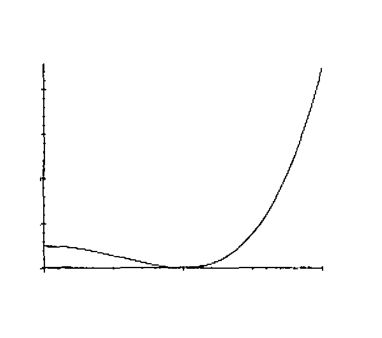
\includegraphics[width=0.40\textwidth]{figs/fig_p024_1.png}
  \caption{势 $V(\rho)$ 的形状：曲线在 $\rho=\rho_0>0$ 处达到极小并触及横轴，向左（$\rho\to0$）略微回升，向右则陡升；纵轴带有分度刻线，原图未标注坐标轴名称与数值。（原文 Figure 1，p.24）}
  \label{fig:p24-1}
\end{figure}

最简单的这类势是 $V(\rho)=\frac18(\rho^2-\rho_0^2)^2$，其极小值在 $\rho_0$ 处。若令 $\Omega=\phi/\rho\in S^2$，我们可以把拉氏量改写为

\[
  \mathcal{L}=\frac1\lambda\int d^nx\Bigl[
  \frac12(\partial_\mu\rho)^2
  +\frac12\rho^2(\partial_\mu\Omega)^2
  +V(\rho)\Bigr].
\]

项 $\frac12\rho^2(\partial_\mu\Omega)^2$ 代表 $S^2$ 上的圆度规（round metric）。

当 $\lambda$ 很小时，我们可以期望经典近似是好的。由于 $\rho$ 是有质量的场，我们可以把它从理论中积掉：令它等于其极小值 $\rho_0$，并研究涨落

\[
  \rho=\rho_0+w,
\]

其中 $w$ 现在是出现在我们路径积分中的量子场。到第一阶近似，我们将有有效拉氏量

\[
  \mathcal{L}_{\mathrm{eff}}(\Omega)=\frac{\rho_0^2}{2\lambda}\int d^nx\,(\partial\Omega)^2,
\]

% [Tutor Note: 由 $\Omega=\phi/\rho$ 到 $\frac12\rho^2(\partial_\mu\Omega)^2$ 这一步用到了 $|\Omega|^2=1$ 的约束：把 $\vec\phi=\rho\,\Omega$ 代入 $\frac12(\partial_\mu\vec\phi)^2$，得 $\frac12(\partial_\mu\rho)^2+\rho\,\partial_\mu\rho\,\Omega\cdot\partial_\mu\Omega+\frac12\rho^2(\partial_\mu\Omega)^2$，其中交叉项因 $0=\partial_\mu(\Omega^2)=2\Omega\cdot\partial_\mu\Omega$ 而消失——这个消去是关键，漏掉它就会多出一个 $\rho\,\partial_\mu\rho\,\Omega\cdot\partial_\mu\Omega$ 型的项。另外注意 $\Omega$ 取值于 $S^2$，故 $(\partial_\mu\Omega)^2$ 必须理解为由 $S^2$ 的圆度规缩并：$g_{ij}(\Omega)\partial_\mu\Omega^i\partial_\mu\Omega^j$，这正是「$\frac12\rho^2$ 是度规的共形因子」一语的含义。]

% ===== 原文 p.25 =====
它描述一个映入 $G/H$ 的非线性 $\sigma$ 模型，在目前情形下 $G/H$ 就是 $S^2$。无质量场由 $\Omega$ 描述。

这能是答案吗？换句话说，是否任何量子场论都能在红外区流向这个 $\sigma$ 模型？事实上，对于时空维数 $n>2$，它确实是一个可能的答案，因为非线性 $\sigma$ 模型在二维以上是不可重整的，所以我们得到的相互作用是无关的。也就是说，若 $a_i$ 是 $S^2$ 上点 $P$ 附近的 Riemann 法坐标（Riemann normal coordinates），我们可以在 $P$ 附近示意地展开

\[
  (\partial\Omega)^2=(da)^2+R\,a^2(da)^2+\cdots
\]

其中 $R$ 是 $S^2$ 的 Riemann 张量。由此我们看到该相互作用在二维以上是无关的。事实上，为给 $(da)^2$ 以维数 $n$，我们必须赋予 $a$ 以维数 $(n-2)/2$，于是该相互作用的维数为 $2n-2$，当 $n>2$ 时超过 $n$。$\sigma$ 模型对 $n>2$ 是可能的答案而对 $n\le2$ 不是，这一点是前面讨论过的事实的另一个侧面：连续对称性的自发破缺对 $n>2$ 可能、对 $n\le2$ 不可能。这一展开也可以作为从 $\sigma$ 模型显式计算 Goldstone 玻色子 $S$ 矩阵的出发点。

% [Tutor Note: 这个展开写得很「示意」，严格的形式是：在法坐标下 $S^2$ 的度规为 $g_{ij}(a)=\delta_{ij}-\frac13R_{ikjl}a^ka^l+O(a^3)$，于是 $(\partial_\mu\Omega)^2=g_{ij}(a)\partial_\mu a^i\partial_\mu a^j=(da)^2-\frac13R_{ikjl}a^ka^l\partial_\mu a^i\partial_\mu a^j+\cdots$；原文把它压缩成 $R\,a^2(da)^2$，其中 $R$ 泛指 Riemann 张量（在 $S^2$ 这一二维情形它只有一个独立分量，正比于曲率标量），系数 $\frac13$ 与四个指标的具体缩并方式被吸收进「$\cdots$」。做量纲计数时还要注意 $(da)^2$ 是 $(\partial_\mu a)^2$ 的缩写（$[\partial_\mu]=1$），故 $[a]=(n-2)/2$，而 $R\,a^2(da)^2$ 的维数为 $-2+2\cdot\frac{n-2}{2}+n=2n-2$，与原文结论一致。]

$\sigma$ 模型是否是我们这个具体问题红外行为的正确答案（至少对足够小的 $\lambda$）？我们断言是的。为研究这一点，让我们微扰地处理 $w$ 的效应。$w$ 与 Goldstone 玻色子的相互作用来自拉氏量中的相互作用项：

\[
\begin{aligned}
  \frac1{2\lambda}\rho^2(\partial\Omega)^2
  &=\frac1{2\lambda}(\rho_0+w)^2(\partial\Omega)^2\\
  &=\frac1{2\lambda}(\rho_0^2+2\rho_0w+w^2)(\partial\Omega)^2.
\end{aligned}
\]

算符 $\partial\Omega$ 是高度非线性的，可以认为它能发射任意多个 Goldstone 玻色子。为了求出有效拉氏量，我们需要计算涉及 $w$ 的费曼图。一个典型的图是

\begin{figure}[htbp]
  \centering
  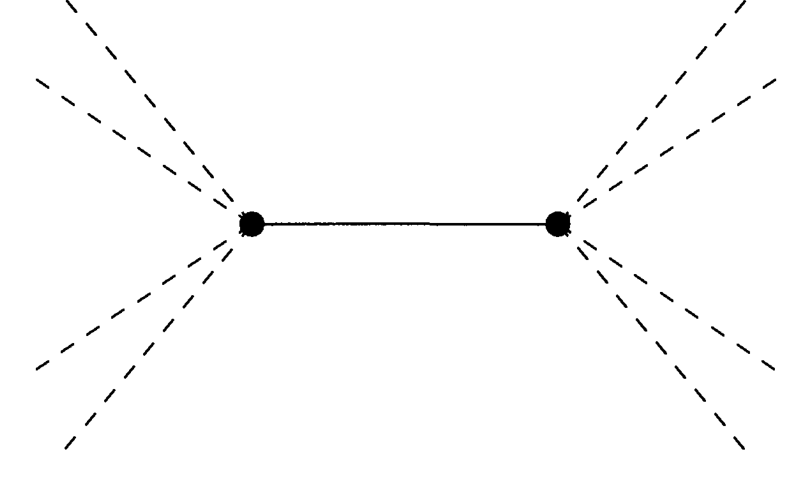
\includegraphics[width=0.60\textwidth]{figs/fig_p025_1.png}
  \caption{$w$ 场的交换图：实线代表有质量的 $w$ 场，虚线代表 $a$（即 $\Omega$ 的涨落，也就是 Goldstone 玻色子）；两个黑点表示来自 $\rho^2(\partial\Omega)^2$ 的顶点，每个顶点各连出四条外线（虚线的多重性来自 $(\partial\Omega)^2$ 的任意阶展开）。（原文 Figure 1，p.25）}
  \label{fig:p25-1}
\end{figure}

这里我们用实线表示 $w$，用虚线表示 $a$。$w$ 的传播子是 $\frac1{k^2+m_w^2}$；由于我们关心小动量 $k$，我们按 $k$ 的幂次展开。领头项是

\[
  \mathrm{const}\cdot(\partial\Omega)^2\frac1{m_w^2}(\partial\Omega)^2.
\]

它具有 $SO(3)$ 对称性，而且是一个无关的相互作用。它甚至比上面草绘的那些来自把 $(\partial\Omega)^2$ 按 $a$ 的幂次展开的项更加无关。

事实上，尽管研究这些图很有教益（哪怕只是为了说明 $\sigma$ 模型是红外稳定的），我们并不需要图的细节。我们所需要知道的只是：有效作用量具有 $SO(3)$ 对称性。给定这一对称性，有效作用量中可能产生哪些项呢？

% ===== 原文 p.26 =====
\begin{itemize}
\item 势 $V(\Omega)$ 不可能出现，因为 $S^2$ 上不存在 $SO(3)$ 不变的函数。这正是给定 $SO(3)$ 对称性后 $\sigma$ 模型红外稳定的基本原因。一个势函数会完全改变图景。例如，一个一般的势会有一个孤立的、非退化的极小值，从而给我们一个唯一的真空以及一个红外平庸的有质量理论，这与自发破缺的 $SO(3)$ 所联系的连续真空族形成对照。
\item 唯一只含两个导数、且尊重问题全部对称性的项就是 $(\partial\Omega)^2$ 本身。（这本质上是因为 $S^2$ 上任何 $SO(3)$ 不变的度规都是标准度规的倍数。）因此，理所当然应当预期：由含 $w$ 场的图带来的量子修正会改变这一项的系数。
\item 其他可能的项，如 $(\partial\Omega^2)^2$ 与 $(\partial\Omega)\nabla^2(\partial\Omega)$，含有多于两个的导数，因而越来越无关。
\end{itemize}

于是，领头的红外行为由形如 $\frac1{f^2}(\partial\Omega)^2$ 的有效作用量决定，其中

\[
  \frac1{f^2}=\frac{\rho_0^2}{2\lambda}+\text{圈修正}.
\]

% [Tutor Note: 上列第三条中的 $(\partial\Omega^2)^2$ 应读作 $((\partial\Omega)^2)^2$：本节末尾讨论 $k^4$ 阶新常数时，作者自己写的就是 $((\partial\Omega)^2)^2$，可见这里是原书排印时少了一层括号（若照字面读成 $(\partial_\mu\Omega^2)^2$，指标根本无从缩并）。同理 $(\partial\Omega)\nabla^2(\partial\Omega)$ 的严格写法是 $\partial_\mu\Omega\,\nabla^2\partial_\mu\Omega$，其中 $\nabla^2=\partial_\nu\partial_\nu$ 作用在第二个因子上。另注意 $f$ 的归一化：此处 $\Omega$ 是无量纲的 $S^2$ 坐标、作用量写作 $\frac1{f^2}(\partial\Omega)^2$，与把 $\pi$ 介子场写成 $\Omega=\exp(2i\pi^a\tau^a/f_\pi)$ 的常见约定相差一个常数因子，故 $f$ 并非通常的衰变常数 $f_\pi$；跨文献比较数值前必须先统一 $\Omega$ 的归一化。]

把这个作用量在某个给定真空（即给定点 $P\in G/H$）附近的 Riemann 法坐标中展开时，就得到涉及 $G/H$ 的 Riemann 张量及其协变导数的相互作用（其中第一个已在上面草绘）。如果用这些相互作用计算涉及小动量（量级为 $k$）的 Goldstone 玻色子的散射振幅，则在 $k$ 接近零时，树图振幅全都正比于 $k^2$，因为相互作用项都恰好含有两个导数。当 $k\to0$ 时圈贡献更小，因为这些相互作用在红外区是无关的。更确切地说，圈图振幅要么 (i) 重整化 $SO(3)$ 不变拉氏量中的常数 $f$，要么 (ii) 给出在 $k\to0$ 时比 $k^2$ 更快趋于零的散射振幅修正。

因此，Goldstone 玻色子散射中 $k^2$ 阶的各项完全由单个常数 $f$ 决定（更一般地说，由齐性空间（homogeneous space）$G/H$ 上一个 $G$ 不变度规的选取决定）。1960 年代人们发现，$\pi$ 介子的低能散射漂亮地符合这样的描述，其中 $G=SU(2)\times SU(2)$，$H$ 是对角的 $SU(2)$。强相互作用具有自发破缺的近似手征对称性（chiral symmetry），就是以这种方式被发现的；这一发现对此后物理学的发展起了非常重要的作用。

如果人们想计算 Goldstone 玻色子散射中比 $k^2$ 更高阶的项，会怎样？显然，在 $k^4$ 阶会有新的常数进入，它们只能由微观计算（或实验）确定，因为存在含四个导数的 $G$ 不变相互作用（例如上面由所考虑的显式树图得到的 $((\partial\Omega)^2)^2$ 项）。然而有趣的是，在四维时空中，Goldstone 玻色子 $k^2$ 振幅的最低阶修正不是 $k^4$ 阶，而是 $k^4\ln k$ 阶。它来自一个圈图，

% ===== 原文 p.27 =====
\begin{figure}[htbp]
  \centering
  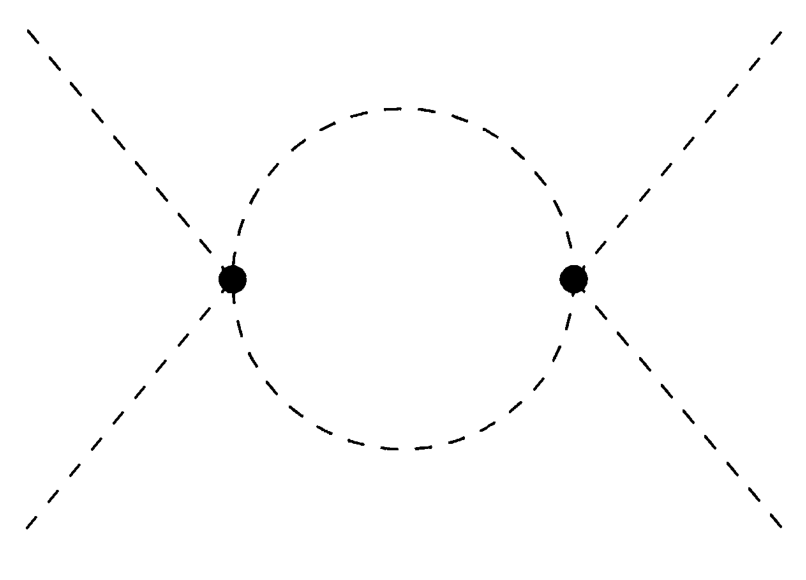
\includegraphics[width=0.56\textwidth]{figs/fig_p027_1.png}
  \caption{给出 $k^4\ln k$ 修正的单圈图：两个顶点取自拉氏量中含两个导数的部分，两个顶点各连出两条外线（虚线），二者之间由两条虚线连成圈（$a$ 场即 Goldstone 玻色子）。（原文 Figure 1，p.27）}
  \label{fig:p27-1}
\end{figure}

其顶点取自拉氏量的两导数部分，因此它完全由控制散射振幅中 $k^2$ 项的那个同一常数 $f$ 唯一确定。

% [Tutor Note: 「$k^4\ln k$ 而非 $k^4$」是量纲分析容易漏掉的一步：树图只有两个导数，故振幅 $\sim k^2$；四导数树图给出 $k^4$，系数是新的自由常数；而这个单圈图的两个顶点各含两个导数，共四个导数，按幂次计数本应为 $k^4$，但在 $d=4$ 时圈积分 $\int d^4q\,\frac{1}{q^2}\frac{1}{(q+k)^2}$ 是临界的，出现 $1/\varepsilon$ 极点，抵消极点后剩下的就是 $\ln k$（红外端由外动量 $k$ 截断），于是量纲上「应该」是 $k^4$ 的项被 $\ln k$ 修饰。这类项被称为手征对数（chiral log）：它的系数不含任何新参数，完全由 $f$ 与 $G/H$ 的曲率固定——这正是低能定理的威力所在，也是流代数能做出可检验预言的原因。]

通过我上面解释的想法对低能 Goldstone 玻色子相互作用所作的分析，被称为「流代数（current algebra）」。特别地，借助流代数关系，人们可以从实验推断破缺对称群 $G$ 是什么，以及 $G$ 不变有效拉氏量中的许多参数。

关于诸如本例这样的对称性破缺例子，最后一点评论：如果我们从一个 $G$ 不变的微观拉氏量 $\mathcal{L}_{\mathrm{micro}}$ 出发，并将其微扰为

\[
  \mathcal{L}_{\mathrm{micro}}+\varepsilon(\delta\mathcal{L}),
\]

其中 $\varepsilon$ 是小参数，且 $\delta\mathcal{L}$ 这一项不是 $G$ 不变的，那么在红外区我们将得到

\[
  \frac1{f^2}(\partial\Omega)^2+\varepsilon V(\Omega)+O(\varepsilon^2),
\]

其中 $V(\Omega)$ 是一个非 $G$ 不变的算符——它最重要的部分当然是不含导数的势，正如记号 $V$ 所提示的。$V(\Omega)$ 受到高度约束，因为它在 $G$ 下必须与 $\delta\mathcal{L}$ 以同样的方式变换。例如，在强相互作用的情形中，确实存在一个小的 $\delta\mathcal{L}$ 项，它把 $SU(2)\times SU(2)$ 破缺到对角 $SU(2)$；它从原本会是连续族的真空中选出一个唯一真空，并给 $\pi$ 介子以小的质量。（关于这一点，详见习题课中的问题 1。）由于 $\pi$ 介子实际上有质量，人们不能把它的四维动量展开到零附近；在 $\pi$ 介子的流代数研究中，实际上取动量 $k$ 为 $\pi$ 介子质量的量级。

\subsection*{参考文献与交叉引用}

关于场论的一般性，特别是对称性这一概念，更多内容见 [I-Classical Fields]（经典）与 [I-Axiomatics]（量子）。§§1.1、1.2 的非微扰估计是瞬子计算的例子，第 7 讲对之讨论得更详细。二维中角值自由场的理论在 [II-CFT] 的第 1 讲以及本系列的第 6 讲中讨论。关于 Goldstone 玻色子是四维中唯一自旋为 $0$ 的无质量粒子的讨论见第 2 讲。场论红外行为的一般性讨论见第 2 讲，后面各讲中有大量例子。这些讲末尾的问题 1 涉及对称性破缺。

% [Tutor Note: [I-Classical Fields]、[I-Axiomatics]、[II-CFT] 是本丛书（\emph{Quantum Fields and Strings: A Course for Mathematicians}）第 I、II 卷中对应章节的代号：I 卷讲经典场论与公理化场论，II 卷含共形场论（CFT）部分；作者用它们代替具体的页数引用。此处「二维中角值自由场」指取值于 $S^1$ 的自由标量场，其顶点算符 $e^{in\varphi(x)}$ 的关联函数按幂律衰减、标度维数与 $n^2$ 成正比，是二维 CFT 的基本构造块，与本讲讨论的 Goldstone 玻色子（取值于 $G/H$ 的非线性 $\sigma$ 模型）在二维的失效密切相关。]

关于二维时空中不存在自发对称性破缺的 Coleman 定理，可见

\begin{quote}
S. Coleman, \emph{There Are No Goldstone Bosons In Two Dimensions}, Commun. Math. Phys. \textbf{31} (1973), 259.
\end{quote}

% ===== 原文 p.28 =====
关于自发破缺的整体对称性及其蕴涵的入门介绍，见

\begin{quote}
S. Coleman, \emph{Aspects Of Symmetry}, Cambridge University Press, 1985.\\
S. Weinberg, \emph{The Quantum Theory Of Fields}, chapter 19, vol. 2, Cambridge University Press, 1996.
\end{quote}


\clearpage
% 原文 pp.29–34（印刷 pp.1147–1152）
\section{Lecture 2：规范对称性破缺与红外行为续论}

\begin{keytakeaways}
本讲从哈密顿途径重新刻画规范场论：位形空间取为运动方程解空间 $\widetilde{M}_0$，物理相空间是辛商 $M=M_0/\!/\widehat{G}_0$，而真正被谈论"破缺"的对称群是无穷远处的常值规范变换群 $G_\infty=\widehat{G}/\widehat{G}_0$。核心数学工具是矩映射 $\mu:M_0\to\widetilde{\mathfrak g}_0^*$ 及其给出的哈密顿量 $Q(\varepsilon)$；用 Noether 形式与 Gauss 约束把 $Q(\varepsilon)$ 化为无穷远处球面上的通量积分，这说明"荷"是由边界（红外）数据决定的。以带复标量的 $U(1)$ 规范场论为例，作者区分了 $v^2>0$（唯一真空、无质量矢量加两个有质量标量）与 $v^2<0$（极小圆、Higgs 机制、全部场有质量）两种情形，并强调规范对称性破缺与整体对称性破缺有本质区别：极小圆上各点彼此规范等价，故只对应一个真空。最后把整体对称性与规范对称性联系起来：若物质拉氏量红外地自由，则"整体对称性破缺"与"规范化后出现 Higgs 机制"互为充要，并开启关于"不存在更高自旋无质量粒子"的一般性讨论。
\end{keytakeaways}

% ===== 原文 p.29 =====
% 原文 §2.1
%（原文标题页：LECTURE 2 / Gauge Symmetry Breaking and More on Infrared Behavior，印刷 p.1147。）
本讲的标题是 \emph{Gauge Symmetry Breaking and More on Infrared Behavior}（规范对称性破缺与红外行为续论）。

\subsection{规范对称性}

回顾规范对称性是什么。我们有时空 $X=\mathbb{R}_{\text{time}}\times X_0$。我们有一个紧致规范群（compact gauge group）$G$。我们有一个场论，其中的场位形（field configuration）是 $\mathbb{R}^d$ 上某个主丛（principal bundle）中的联络（connection），此外还可能有某些物质场（matter fields）。

回顾规范场论的哈密顿途径（Hamiltonian approach）。设 $\widetilde{M}_0$ 为经典运动方程的解所构成的空间。在 $\widetilde{M}_0$ 上有规范变换群 $\widehat{G}$ 的作用。设 $M_0\subset\widetilde{M}_0$ 为满足下述条件的全部解构成的空间：$G$-丛在时间方向上被平凡化，并且联络在该方向上为平凡。这类解一如往常完全由 $A(t_0)$、$\frac{dA}{dt}(t_0)$ 这一对数据（其中 $t=t_0$ 是一个空间切片）连同物质场的初始数据所决定。显然（It is clear that），$\widetilde{M}_0$ 的任一元素都可以借规范变换化到 $M_0$ 中，因此 $M_0$ 在规范变换的意义下仍然包含全部解。

% [Tutor Note: 作者说"显然"，实则用到两件事：(i) 时空取乘积形式 $X=\mathbb{R}_{\text{time}}\times X_0$，时间方向可缩，故任何主丛沿时间方向可平凡化；(ii) 丛平凡化后，沿 $t$ 解常微分方程 $\frac{dg}{dt}g^{-1}=-A_t$ 即可把 $A_t$ 规范掉。若时空不是乘积（例如含非平凡的时间方向缠绕），这一步不成立，$M_0$ 便不能捕获全部解。]

设 $X_0=\mathbb{R}^{d-1}$。此时我们可以只考虑平凡丛，并且（若能量有限）只考虑在空间无穷远处为平凡的联络。换言之，若 $\mathcal{A}$ 是 $\mathbb{R}^{d-1}$ 上平凡 $G$-丛的、在 $\infty$ 处为平凡的联络 $A$ 所构成的空间，则纯规范场论的 $M_0$ 就是 $T^*\mathcal{A}$。若存在物质场，则 $M_0$ 是 $T^*\mathcal{A}$ 与某个别的空间的乘积。

定义 $\widehat{G}$ 为 $\mathrm{Maps}(\mathbb{R}^{d-1},G)$ 中在无穷远处有极限的那些元素所构成的群，并定义 $\widehat{G}_0$ 为 $\widehat{G}$ 中在 $\infty$ 处趋于 $1$ 的函数所构成的子群。我们有 $\widehat{G}/\widehat{G}_0=G$。这个商群称为无穷远处的常值规范变换群（group of constant gauge transformations at $\infty$），并记作 $G_\infty$。

% [Tutor Note: 原文同一页内对规范变换群的记号在 $\widehat{G}$ 与 $\widetilde{G}$ 之间摇摆（"the group $\widehat G$ of gauge transformations" 与 "Define $\widetilde G$ to be the group of elements of $\mathrm{Maps}(\mathbb{R}^{d-1},G)$"）；扫描件上宽帽与波浪号极易混淆，本译文统一记作 $\widehat{G}$、$\widehat{G}_0$（解空间则统一记作 $\widetilde{M}_0$）。另需注意 $\widehat{G}/\widehat{G}_0\cong G$ 之所以成立，是因为"在 $\infty$ 处趋于 $1$"的映射群 $\widehat{G}_0$ 可缩（$G$ 连通时），故商群只由无穷远处的极限值决定；若 $X_0$ 不单连通（如二维涡旋或三维磁单极子的情形），$\pi_1$ 部分会额外贡献拓扑荷，此时商群不再是单纯的 $G$。]

群 $\widehat{G}$ 在 $M_0$ 上辛作用（acts symplectically）。规范场论中的物理相空间是辛商（symplectic quotient）$M=M_0/\!/\widehat{G}_0$。注意我们只对 $\widehat{G}_0$ 取商，而不对整个群 $\widehat{G}$ 取商，于是商群 $G_\infty$ 在 $M$ 上的作用被继承下来。我们要讨论的正是这个对称群的破缺。

% 原文 §2.2
\subsection{规范对称性破缺与无穷远处的荷}

\textbf{定义（Definition）}。设我们有一个（经典）规范场论，$s\in M$ 是它的真空态。设 $H\subset G=G_\infty$ 是 $s$ 的稳定化子（stabilizer）。此时我们说：在基态 $s$ 处，规范对称性由 $G$ 破缺到 $H$。

\footnote{本讲笔记由 Pavel Etingof、David Kazhdan 与 David Morrison 整理。（原文 p.1147 页脚注）}

% ===== 原文 p.30 =====
因此，所谓对称性破缺，其含义大体上（roughly）与整体对称性的情形相同：$M$ 上函数所成泊松代数（Poisson algebra）有一个对称性，它不固定某个特定的基态。

\textbf{重要评注（Important remark）}。上面"大体上相同"这一说法必须极其小心地对待。两种情形之间存在若干根本性的区别，这些区别将在下文变得清楚。它们来自这样一个事实：在我们此处所考虑的情形中（与第 1 讲不同），物理可观测量按定义是规范不变的，因而自动与 $G$ 对易，从而不能分辨 $M$ 上的点；也就是说，并非 $M$ 上的每个函数都是"可观测的"。换句话说，$G$ 对"理论"（第 1 讲意义下的理论）的作用从一开始就是平凡的。与此相关：我们在第 1 讲中对整体对称性自发破缺（spontaneous symmetry breaking）的表述在抽象意义上是自洽的，但我们在此处所表述的规范对称性自发破缺这一概念，却系于一个底层的经典描述。

上述评注的一个变体是：「规范对称性破缺」（gauge symmetry breaking）这个说法其实并不指某种可以用抽象、公理化方式加以描述的现象。它指的是某个特定的重要现象，称为 Higgs 机制（Higgs mechanism），它出现在某些弱耦合规范场论中。下面我们用例子来说明这一机制。

现在我们（在经典层面）计算 $G$ 的作用。首先我们有一个矩映射（moment map）$\mu:M_0\to\widetilde{\mathfrak g}_0^*$，其中 $\widetilde{\mathfrak g}_0$ 是 $\widehat{G}_0$ 的李代数——即从 $\mathbb{R}^{n-1}$ 到 $G$ 的李代数 $\mathfrak g$ 的、在无穷远处为零的函数所构成的代数。于是，对任意 $\varepsilon\in\widetilde{\mathfrak g}_0^*$，我们有哈密顿量 $Q(\varepsilon)\in C^\infty(M_0)$，由 $Q(\varepsilon)(X)=\mu(X)(\varepsilon)$ 定义。

% [Tutor Note: 此处指标有笔误之嫌：$\mu$ 取值于对偶空间 $\widetilde{\mathfrak g}_0^*$，而配对写作 $\mu(X)(\varepsilon)$，则 $\varepsilon$ 应属于 $\widetilde{\mathfrak g}_0$ 而非 $\widetilde{\mathfrak g}_0^*$；"for any $\varepsilon\in\widetilde{\mathfrak g}_0^*$" 与 $\mu(X)(\varepsilon)$ 类型不匹配。理清这一点的办法是把 $\mu(X)\in\widetilde{\mathfrak g}_0^*$ 与 $\varepsilon\in\widetilde{\mathfrak g}_0$ 作自然配对；本译文照原文抄录，读者按此理解即可。]

事实上，用 Noether 形式很容易算出 $Q(\varepsilon)$。即

\begin{equation}
  \tag{2.1}
  \label{eq:2-1}
  Q(\varepsilon)=\int_{\mathbb{R}^{d-1}}\operatorname{Tr}\left(\frac{dA}{dt}\nabla_A\varepsilon\right)d^{d-1}x+\text{物质场项},
\end{equation}

在 $M$ 上，若 $\varepsilon$ 在无穷远处为零，则 $Q(\varepsilon)=0$。因此，在 $M$ 上有 $\nabla_A^*\frac{dA}{dt}=$ 物质场项。特别地，在纯规范场论中 $\nabla_A^*\frac{dA}{dt}=0$。

% [Tutor Note: 这里由 (2.1) 得到 Gauss 约束是一步被压缩的推导。关键是对 $\int\operatorname{Tr}\left(\frac{dA}{dt}\nabla_A\varepsilon\right)$ 作分部积分：$\nabla_A^*$ 是 $\nabla_A$ 关于 $\int\operatorname{Tr}(\,\cdot\,\cdot\,)$ 的形式伴随，故 $\int\operatorname{Tr}(\dot A\nabla_A\varepsilon)=-\int\operatorname{Tr}\left(\varepsilon\nabla_A^*\dot A\right)+(\text{无穷远边界面项})$。当 $\varepsilon$ 于 $\infty$ 处为零时边界面项消失，于是"$Q(\varepsilon)=0$ 对一切此种 $\varepsilon$ 成立"等价于 $\nabla_A^*\dot A=0$（有物质场时为 $\nabla_A^*\dot A=j$）。指标上易错之处是 $\nabla_A^*$ 作用在取值于 $\mathfrak g$ 的 $(d-1)$ 维空间 1-形式 $\dot A$ 上给出标量，其显式为 $-g^{ij}(\partial_i\dot A_j+[A_i,\dot A_j])$，符号约定不同会使 Gauss 约束差一个整体号。]

把这一点考虑进去，我们看到在 $M$ 上有

\begin{equation}
  \tag{2.2}
  \label{eq:2-2}
  Q(\varepsilon)=\int_{\mathbb{R}^{d-1}}\operatorname{Tr}\left(\nabla_A\left(\varepsilon\frac{dA}{dt}\right)\right)d^{d-1}x.
\end{equation}

利用 Stokes 公式，我们可以把 (2.2) 改写成

\begin{equation}
  \tag{2.3}
  \label{eq:2-3}
  \begin{split}
    Q(\varepsilon)&=\lim_{r\to\infty}\int_{S^{n-2}(r)}*_{d-1}\operatorname{Tr}\left(\varepsilon\frac{dA}{dt}\right)\\
    &=\lim_{r\to\infty}\int_{S^{n-2}(r)}*_d\operatorname{Tr}(\varepsilon F),
  \end{split}
\end{equation}

其中 $F$ 是相应于 $M_0$ 中给定点的那个时空联络的曲率，$S^k(r)$ 是半径为 $r$ 的 $k$ 维球面。这个公式定义了 $G=G_\infty$ 在 $M$ 上作用的哈密顿量。

% [Tutor Note: (2.1)–(2.3) 中时空维数的记号并不统一：被积测度写作 $d^{d-1}x$、积分域写作 $\mathbb{R}^{d-1}$（用 $d$），而 (2.3) 的球面写作 $S^{n-2}(r)$、末段又写 $F=o(r^{2-n})$（用 $n$）。自洽的读法是取 $n=d$：空间维为 $n-1=d-1$，其边界为 $S^{n-2}=S^{d-2}$，而 $r^{2-n}$ 正是 $n$ 维时空中 $1/r^{n-2}$ 型通量衰减的判据（$n=4$ 时即 $o(r^{-2})$，对应 $1/r^2$ 的通量，恰为点电荷的库仑场）。切勿把 $S^{n-2}$ 误抄成 $S^{d-2}$ 与 $r^{2-d}$ 混用，否则前后不自洽。]

这个公式表明：若在某状态上 $F=o(r^{2-n})$（$r\to\infty$），则对该状态而言，$Q(\varepsilon)$ 对一切规范变换（不必在无穷远处为零）都为零。然而，若情形并非如此，则对常值 $\varepsilon$，$Q(\varepsilon)$ 可以不为零。

% ===== 原文 p.31 =====
\textbf{例（Example）}。考虑一个含带电复标量的 $U(1)$ 规范场论。其中的场是一个 Hermite 线丛上的联络 $A$，以及该丛的一个截面 $\phi$。拉氏量为

\[
  \mathcal{L}=\frac{1}{4e^2}\int F\wedge *F+\int|D_A\phi|^2d^4x+\int\frac{\lambda}{8}(|\phi|^2+v^2)^2d^4x.
\]

这是四维中由这些场所能写出的最一般的可重整化拉氏量，它在 $\phi\to-\phi$ 下是对称的。这里 $e,\lambda,v$ 是参数，$e^2,\lambda$ 为正，而 $v^2$ 可正可负。为简单起见，我们先假定 $v^2\neq0$。

% [Tutor Note: 三处易错。(i) 原文把这个泛函记作 $\mathcal{L}$，但每一项都已对时空积分，故它实际上是作用量 $S$；下文 (2.4)、(2.5) 同样如此，读谱时不能把它当成拉氏量密度。(ii) 第一项 $\frac{1}{4e^2}\int F\wedge *F$ 中，在欧氏约定下 $F\wedge *F=F_{\mu\nu}F^{\mu\nu}d^4x$；若换用常见的闵氏写法 $-\frac{1}{4e^2}\int F_{\mu\nu}F^{\mu\nu}$，则整项差一个负号，会连带改变 (2.4) 中各质量项的符号约定。(iii) 势为 $\frac{\lambda}{8}(|\phi|^2+v^2)^2$，其极小条件是 $|\phi|^2=-v^2$：$v^2>0$ 时唯一极小在 $\phi=0$，$v^2<0$ 时极小圆为 $|\phi|=b$（$b^2=-v^2$）。这里的加号若误抄成 $(|\phi|^2-v^2)^2$，两种情形的结论会整体对调。]

在四维中，人们不相信这个理论在紫外（UV）存在，但我们将把它视为某个更基本理论的有效理论（effective theory）（或者我们也可以考虑少于四维的情形）。

在经典层面（而当 $e^2,\lambda$ 足够小时在量子层面），我们有两种情形。

\begin{enumerate}
  \item $v^2>0$；势有唯一的极小。
  \item $v^2<0$；势有一个极小圆（circle of minima）。
\end{enumerate}

让我们考察在这两种情形下理论在红外（infrared）中的行为。

\begin{figure}[htbp]
  \centering
  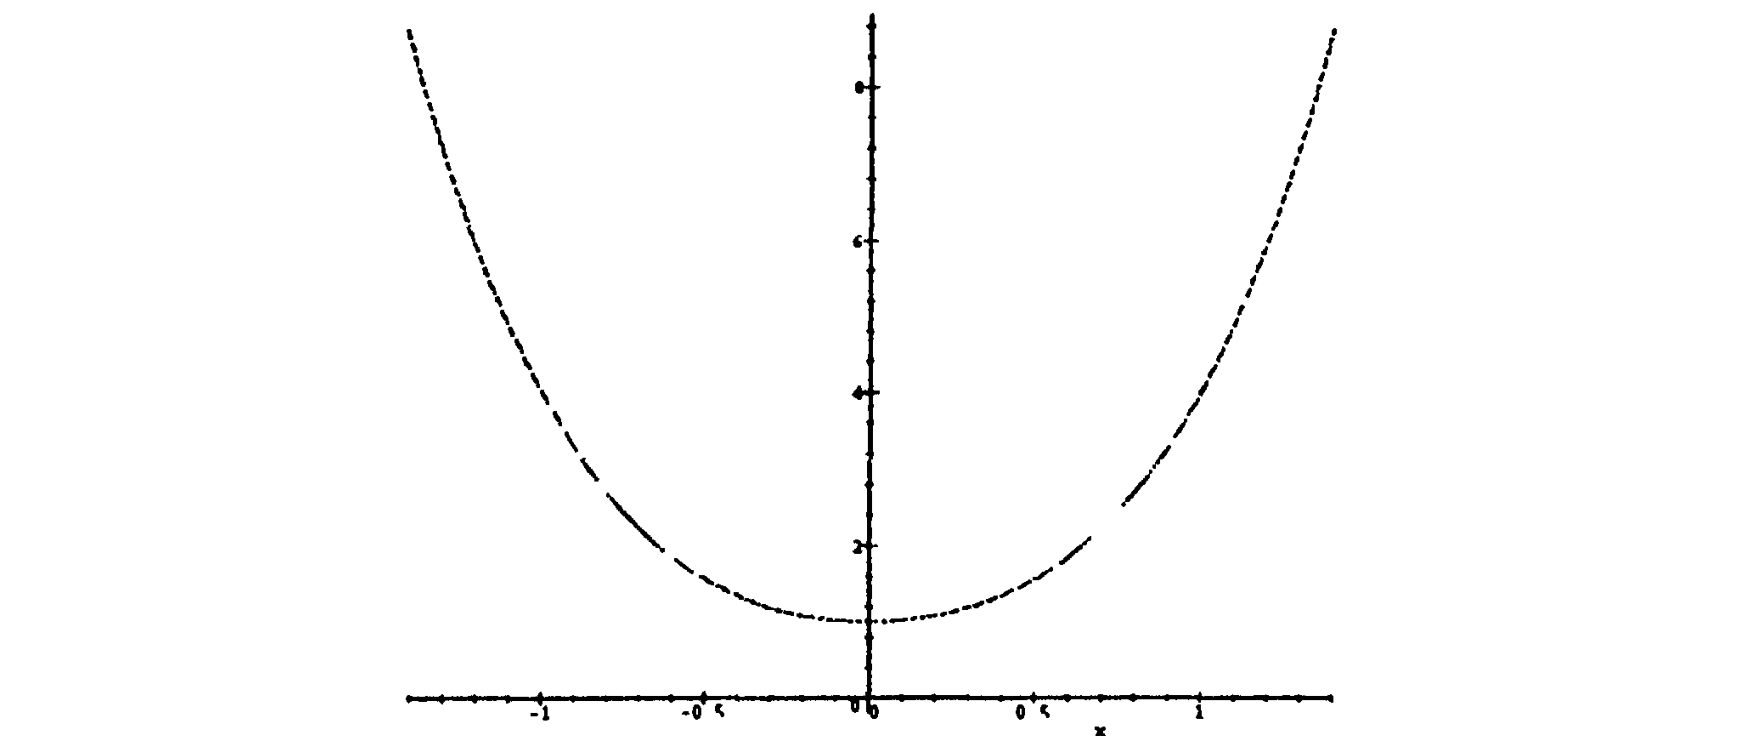
\includegraphics[width=0.72\textwidth]{figs/fig_p031_1.png}
  \caption{$v^2>0$ 时的势能曲线：曲线在原点有唯一极小，横轴为场 $\phi$（图中标为 $x$），纵轴为势能 $V$。（原文 Figure 1，p.31）}
  \label{fig:p31-1}
\end{figure}

\textbf{情形 1（Case 1）}：$v^2>0$。此时能量的极小在 $\phi=0$ 处达到。先考虑规范耦合为零的情形：$e^2=0$。此时我们的理论是纯（自由）阿贝尔规范场论与 $\phi^4$ 理论的直积。因此它有唯一的真空，而出现在谱的下部的粒子是一个无质量矢量，即规范玻色子（gauge boson，来自规范场论），以及两个有质量的实标量（来自 $\phi^4$ 理论）。

若我们把 $e^2$ 取为小的非零值，情况应保持不变。的确，有质量的标量肯定不会发生任何变化（Hilbert 空间中由带非零电荷的态——如这些标量——所构成的子空间在最低阶近似下有质量间隙（mass gap），而"有质量"是一个开条件（open condition））；此外，它们的质量必须相等，因为无穷远处存在一个 $U(1)$ 对称性（即常值 $\varepsilon$ 对应的 $Q(\varepsilon)$），它禁止质量不等。$Q(\varepsilon)\neq0$ 这一点是清楚的，因为在 $e^2=0$ 时就是如此，而此时 $Q(\varepsilon)$ 表示的正是 $U(1)$ 整体对称性。当 $\varepsilon$ 取单位切向量时，算符 $Q(\varepsilon)$ 称为电荷算符（operator of electric charge）。

此外，无质量矢量不可能变成有质量的。的确，回忆一下：无质量矢量意味着 $SO(3,1)$ 的一个不可约表示，其 $p^2=0$、自旋为 $1$，亦即光锥（light cone）上一个二维等变向量丛（equivariant vector bundle）的截面空间。这个向量丛不可能形变为双曲面（hyperboloid）上的等变向量丛，

% ===== 原文 p.32 =====
因为双曲面（hyperboloid）上一点的稳定化子群 $SO(3)$ 没有二维不可约表示。因此，小耦合下的量子理论将具有同样的粒子——两个有质量标量（$\phi$ 的实部与虚部）和一个无质量矢量（规范玻色子）。

% [Tutor Note: 这段"不可形变"论证的表示论内核值得点明：$p^2=0$ 时的小群（little group）是 $ISO(2)$，无质量自旋 1 的二维自由度来自其转动子群 $SO(2)$；而 $p^2=m^2>0$（"双曲面"即质量壳）时小群是 $SO(3)$，有质量自旋 1 需要三维表示。作者以"$SO(3)$ 没有二维不可约表示"来表述"不能连续形变"，本质上是说无质量矢量要获得质量必须多出一个纵向自由度，而该自由度只能来自别处（在 Higgs 机制中正来自标量）。此处 $SO(3,1)$ 的等变丛语言是把表示论陈述翻译成拓扑陈述，注意"光锥上二维"与"双曲面上三维"的维数差正是纵向自由度。]

\textbf{评注（Remark）}。上述关于无质量矢量不可形变的论证在二维或三维中失效。例如在三维中，无质量矢量恰好是锥上的函数空间，而它可以成功地形变为双曲面上的函数空间。当人们在纯 $U(1)$ 规范场论中引入 Chern–Simons 项 $c\int A\wedge dA$ 时，这确实会发生。理论仍保持自由，但变成有质量的，给出一个有质量标量。在我们所考虑的理论中（就三维而言），这不可能动力学地发生，因为 Chern–Simons 项在改变定向时变号；但在别的理论中这可以发生。

事实上，在量子理论中算符 $Q(\varepsilon)$（对 $\varepsilon$ 作适当归一化后）具有整特征值，因而（在量子理论中）定义了相应 Hilbert 空间的 $\mathbb{Z}$-分次（$\mathbb{Z}$-grading）。特别地，由于 $Q(\varepsilon)\neq0$，而 $Q(\varepsilon)$ 与一切局域算符对易，Hilbert 空间存在一些扇区（即 $Q(\varepsilon)$ 非零的那些扇区），它们不能通过作用局域算符从真空到达。这表明我们根本性地违反了 Wightman 公理：算符代数在物理 Hilbert 空间中的表示不是不可约的。然而，理论仍然只有一个真空：$Q(\varepsilon)$ 非零的扇区中的最低能量为正。

\begin{figure}[htbp]
  \centering
  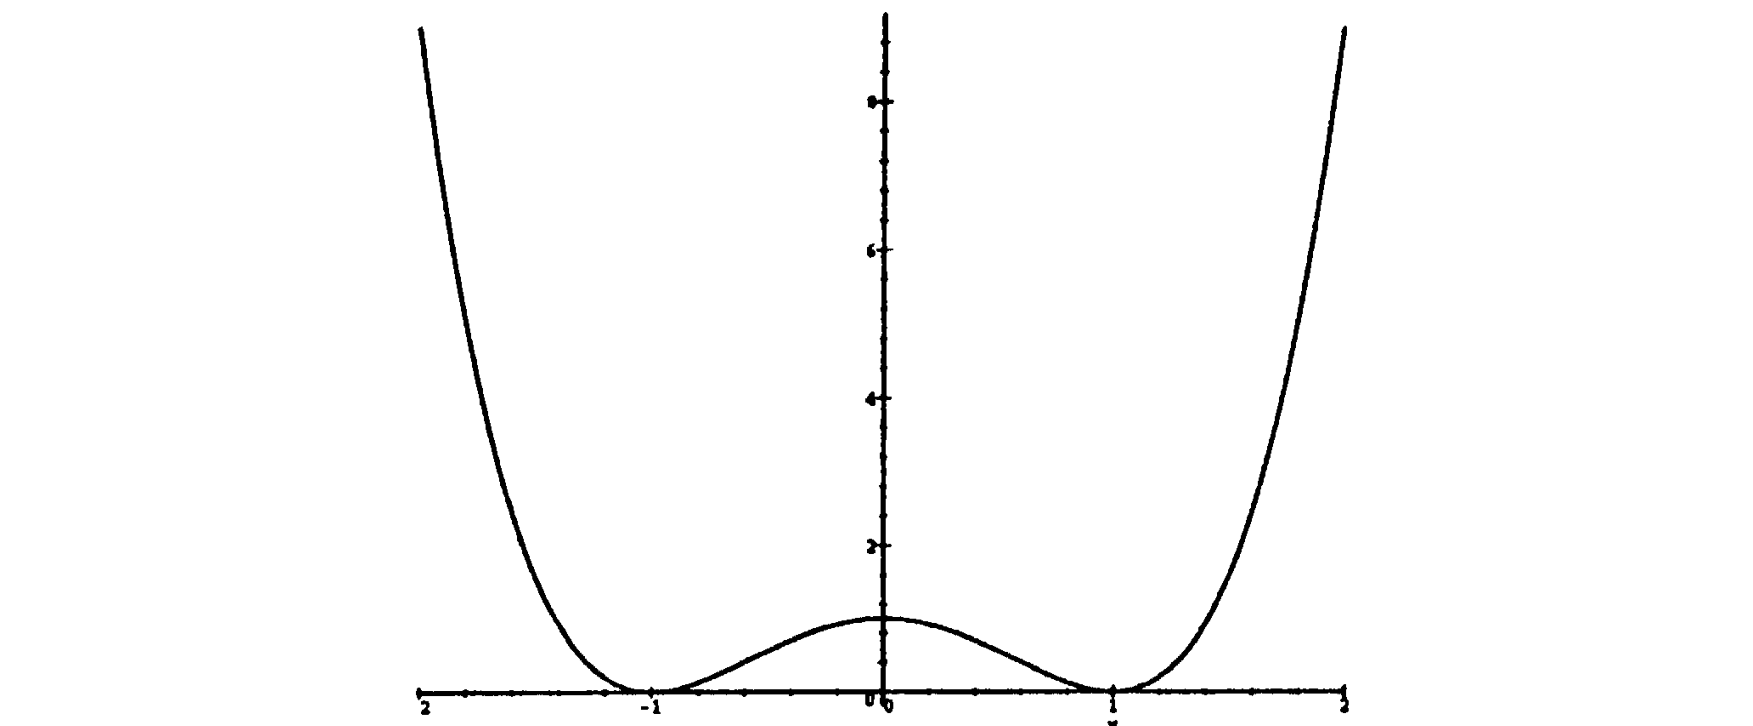
\includegraphics[width=0.72\textwidth]{figs/fig_p032_1.png}
  \caption{$v^2<0$ 时的势能曲线（"墨西哥帽"的截面）：两个简并极小位于 $|\phi|=b$ 处，横轴为场 $\phi$ 的实部（图中标为 $x$），纵轴为势能 $V$。（原文 Figure 2，p.32）}
  \label{fig:p32-1}
\end{figure}

\textbf{情形 2（Case 2）}：$v^2<0$。令 $v^2=-b^2$。那么经典上能量的极小在圆 $|\phi|=b$ 上达到。这意味着任何有限能量位形在无穷远处都具有性质 $\phi=be^{i\theta_0}$，其中 $\theta_0$ 是常数。因此，通过一个在无穷远处有有限极限的规范变换，我们可以安排 $\phi$ 为实且为正：$\phi=b+w$，其中 $w$ 是新的实变量。用这些新变量写出拉氏量，我们将得到如下形式的二次部分：

\begin{equation}
  \tag{2.4}
  \label{eq:2-4}
  L_{\text{quadratic}}=\frac{1}{4e^2}\int F^2+\int d^4x\left((dw)^2+M^2w^2\right)+\int d^4x\,b^2A^2.
\end{equation}

% [Tutor Note: 由 (2.4) 可以反推作者对协变导数的约定。$|D_A\phi|^2$ 在 $\phi=b$ 处给出规范场质量项：若用通常的 $D_A=\partial+ieA$，该项应为 $e^2b^2A^2$，而 (2.4) 中系数恰为 $b^2$，说明作者把电荷 $e$ 吸收进了 $A$（即 $D_A=\partial+A$），或者此处为示意性写法。读质量谱时必须先把 $A$ 归一到标准动能项 $\frac{1}{4}F^2$（即 $A\to eA$），此时 $A^2$ 系数变为 $e^2b^2$，与 $\frac{1}{4}F^2+\frac12m_A^2A^2$ 相比得 $m_A^2=2e^2b^2$。同理，$M^2$ 与 $\lambda b^2$ 同阶：把 $\frac{\lambda}{8}(|\phi|^2-b^2)^2$ 在 $\phi=b+w$ 处展开得 $\frac{\lambda}{2}b^2w^2$，与 (2.4) 中 $M^2w^2$ 对照即可定出 $M^2$。]

由 (2.4) 可见，现在所有场都是有质量的。当然，拉氏量 (2.4) 对 $A$ 不再规范不变，因为我们已经把规范对称性"用掉"以使得 $\phi$ 为实。

因此，对于小的耦合值，相应量子理论的红外极限是平凡的。特别地，不存在无质量规范玻色子：它们

% ===== 原文 p.33 =====
已被 $\phi$ 场"吃掉"（eaten）。这种情形称为 Higgs 现象（Higgs phenomenon），或规范对称性的自发破缺。

注意，尽管存在看起来像零能量态圆圈的东西，我们的理论仍然只有一个真空。换句话说，圆上所有的点被视为同一个态，理由是它们彼此规范等价，因而定义等价的实现（即给出相同的规范不变局域算符的期望值）。这是规范对称性破缺与整体对称性破缺之间的根本区别。在整体对称性破缺中，圆上的点代表理论的不同真空（不同实现），因为存在非对称的算符，它们在该圆的不同点上取不同的期望值。

总结起来，「规范对称性破缺」一语主要指 Higgs 机制，即 Higgs 现象：在诸如 $v^2<0$ 这样的模型中，规范场尽管耦合很弱也获得质量。在严格得多的条件下（见第 10 讲），人们可以对"Higgs 相"的含义给出公理化的解释。但就这个术语最常用的意义而言，「Higgs 机制」不过是即便耦合很弱也能得到有质量谱（或至少使无质量自旋 1 场的数目小于规范群维数）的一条途径。它之所以重要，是因为它是规范场论所能做的最简单的事情之一，而且它在自然界中出现在弱相互作用里。

\textbf{评注（Remark）}。若有人试图用公式 (2.3) 计算情形 2（对称性破缺时）的 $Q(\varepsilon)$，答案将是零，因为被积函数在无穷远处迅速衰减。当 Higgs 机制发生时，与规范对称性相联系的守恒荷为零。

% [Tutor Note: "荷为零"与 (2.3) 的边界积分一致：在 Higgs 相中 $F$ 以 $e^{-m_Ar}$ 指数衰减（$m_A$ 为规范玻色子质量），故 $r\to\infty$ 时球面积分趋于零，$G_\infty$ 的生成元在真空上实现为零。这与电动力学中"总电荷由无穷远 Gauss 通量给出"完全一致：场被屏蔽后通量为零。反过来，情形 1 中 $F\sim Q/r^{2}$ 衰减恰好使 (2.3) 给出非零常数，这正是电荷算符的边界定义。]

在情形 2 下于红外中出现的粒子，按照 (2.4)，是一个有质量矢量（$A$）和一个有质量标量（$\phi$）。只有一个标量，因为 $\phi$ 现在是实的。因此，在表示论的层面上，情形 2 中出现的 Higgs 现象归结为 Poincaré 群表示的一种形变：无质量矢量加无质量标量形变为一个有质量矢量。作为对照，回忆一下：单独一个无质量矢量不能形变为有质量表示。

最后，考虑特殊情形 $v^2=0$。此时经典上我们与 $v^2>0$ 时一样没有对称性破缺，粒子是一个无质量矢量和两个无质量标量。然而，这不应是量子答案，因为此位形在微扰下不稳定。

% [Tutor Note: 作者说 $v^2=0$ 的位形"在微扰下不稳定"，略去了依据。其一是树级势 $\frac{\lambda}{8}|\phi|^4$ 在原点处二阶导数为零，$\phi=0$ 只是高阶临界点，任何微小扰动（包括圈修正）都会移动真空；其二是量子修正会生成 Coleman–Weinberg 型有效势，其中规范场圈给出 $\sim e^4|\phi|^4\ln(|\phi|^2/\mu^2)$ 的项，使原点变成极大值、真空移到 $\langle|\phi|\rangle\neq0$ 处（即量纲穿越，dimensional transmutation）。参见 Sidney Coleman 与 Eric Weinberg, Phys. Rev. D7 (1973) 1888。]

\textbf{评注（Remark）}。如果我们出发的拉氏量不是红外地自由的（IR free），比如说它是某个渐近自由（asymptotically free）规范场论的拉氏量，那么上面讨论的经典分析在量子理论中不适用。此时理论的红外行为一般难以确定。各种事情都可能发生，其中一些我们将在本学期我后续的讲课或 Seiberg 的讲课中听到。除其他可能性外，人们可以以远比 Higgs 机制更奇特、更难理解的方式得到有质量谱；或者人们可以在红外中生成一个并非原经典规范对称性子群的未破缺规范对称性。

% ===== 原文 p.34 =====
% 原文 §2.3
\subsection{对称性破缺与规范化}

最后，让我们讨论整体对称性破缺与规范对称性破缺之间的联系。设我们有一个场论的拉氏量 $L$（譬如在四维中），它具有整体 $U(1)$ 对称性。一个典型的例子是：理论包含一些标量场 $\phi_j$，它们是 Hermite 向量丛的截面，而 $U(1)$ 通过这些截面的乘法 $e^{in_j\theta}$ 作用。通过引入 $U(1)$ 规范场 $A$ 与新的拉氏量，这个 $U(1)$ 对称性可以被规范化（gauged）：

\begin{equation}
  \tag{2.5}
  \label{eq:2-5}
  L_{\text{gauged}}=\frac{1}{4e^2}\int F_A\wedge *F_A+L_A,
\end{equation}

其中 $L_A$ 由原来的物质拉氏量 $L$ 把 $\phi_j$ 的所有导数替换为协变导数（covariant derivative）而得到。

% [Tutor Note: 电荷 $n_j$ 必须是整数，$e^{in_j\theta}$ 才在 $\theta\to\theta+2\pi$ 下良定义，这也保证了 (2.5) 中 $F_A\wedge *F_A$ 的 $1/4e^2$ 归一化在 $U(1)$ 丛的整系数下自洽。另注意 $L$ 与 $L_{\text{gauged}}$ 都不是拉氏量密度而是作用量（同 p.31 的 $\mathcal{L}$），故 $L_A$ 中"替换导数"应理解为对整个作用量中的 $\partial_\mu\phi_j\to D_\mu\phi_j=(\partial_\mu+in_jA_\mu)\phi_j$。]

上述论断是：若 $L$ 是红外地自由的，则在三维以上、小规范耦合下，由 $L$ 与 $L_{\text{gauged}}$ 所定义的两个理论的对称性破缺行为相同。（在二维或三维中讨论需要一些修改，原因是 $U(1)$ 规范场论中的"禁闭"（confinement），我们将在本学期稍后研究它；此外还有某些其他原因，将在今天稍后以及以后的讲课中讨论。）也就是说，若 $L$ 有整体对称性破缺，则 $L_{\text{gauged}}$ 有 Higgs 机制；反之亦然。

的确，让我们考虑两种情形。

\textbf{情形 1（Case 1）}：无整体对称性破缺。我们假定理论足够一般（generic），使得没有无质量带电标量。（这在我们上面的例子中相当于避开临界情形 $v=0$。）在 $e$ 小的极限下，Hilbert 空间是量子化 $L$ 所得的 Hilbert 空间 $\mathcal{H}_L$ 与一个自由无质量自旋 1 场的 Hilbert 空间 $\mathcal{H}'$ 的张量积。$U(1)$ 非平凡地作用，其作用实现于 $\mathcal{H}_L$ 上。在缺少带电无质量标量的情况下，这个含一个无质量自旋 1 场的谱是稳定的；对足够弱的耦合，它不会发生任何变化。

\textbf{情形 2（Case 2）}：整体对称性破缺。此时在能量的极小处，带电场 $\phi_j$ 不为零。不存在不变的经典基态，并且存在一个与这个对称性破缺相应的 Goldstone 玻色子。在此情形下，取一个真空态以及一个在该真空中不为零的分量 $\phi_j^{(n)}$。在规范化的理论中，我们可以作一个规范变换，使这个分量为实且为正。这表明：若不存在其他无质量粒子（特别地，没有其他破缺的整体对称性），则理论中所有的场都将变成有质量的。于是我们得到规范对称性的破缺。在描述这一情形时，我们使用了经典语言，假定了 $L$ 弱耦合；但这一讨论可以抽象地进行，只需假定 $L$ 所描述的理论中 $U(1)$ 对称性是自发破缺的。

这些考虑只在规范耦合小时成立。（若我们在四维取非阿贝尔规范群，那么在情形 1 中还有进一步的限制：只有当 $\beta$ 函数为正、从而规范耦合在红外流向零时，这一分析才适用。）

% 原文 §2.4
\subsection{不存在更高自旋的无质量粒子}

现在我们对四维的红外地自由理论作一般的考察。（以下的考虑可推广到四维以上，但在四维以下会变得平凡……）

% 说明：本句在原文 p.1153 续完（"… below four dimensions"），其内容属于第二部分（p.35 起）。

% 原文 pp.35–39（印刷 pp.1153–1157）

% ===== 原文 p.35 =====
% [承接 p.34 末句「The considerations that follow generalize above 4 dimensions but become trivial below dimension 4).」]
维数 4）。
对庞加莱代数（Poincaré algebra）的表示、以及各种自旋的自由场作一般讨论，似乎提示红外自由（infrared-free）的理论可以有任意自旋的无质量粒子。
但在实际上，在我所熟悉的一切有趣例子中，都可以先验地（\textit{a priori}）论证：任何无质量粒子都只能有自旋 $0$、$1/2$ 或 $1$。

我们关心的大多数理论，不仅可以表述在平坦的 $\mathbb{R}^4$ 上，而且可以表述在带有一般度规 $g$ 的更一般的弯曲四维流形 $M^4$ 上。
事实上，任何构成对自然之描述的一部分的理论都具有这一性质，因为广义相对论是自然的一部分，而在广义相对论中时空是弯曲的！
在量子场论中，能够在弯曲时空上工作，意味着存在一个非常特殊的算符，称为应力张量（stress tensor）或能量—动量张量（energy-momentum tensor）$T_{\mu\nu}(x)$。
它度量理论对度规张量 $g$ 之改变的响应。
我们假定理论由拉格朗日量 $\mathcal{L}(\phi_i;g)$ 在一般的 $g$ 下表述，而该量在同时作用于 $\phi_i$ 与 $g$ 的微分同胚（diffeomorphism）下不变。
$g$ 不是理论的场之一——它是任意的，但在研究 $\phi_i$ 的经典或量子动力学时被固定——而这种微分同胚不变性意味着：理论若表述于时空 $(M,g)$ 之中，则它实际上只依赖于 $g$ 的微分同胚类。
在此框架下，应力张量定义为
\[
  T_{\mu\nu}=\frac{\delta\mathcal{L}}{\delta g^{\mu\nu}}.
\]
这显然（obviously）蕴含 $T$ 是对称张量
\[
  T^{\mu\nu}=T^{\nu\mu}.
\]

% [Tutor Note: 此处定义 $T_{\mu\nu}=\delta\mathcal{L}/\delta g^{\mu\nu}$ 省略了两处约定，照抄极易出错。(i) 常规的广义相对论约定是 $\delta S=\frac12\int d^4x\sqrt{g}\,T^{\mu\nu}\,\delta g_{\mu\nu}$，其中带 $\frac12$ 与 $\sqrt{g}$；作者的 $\mathcal{L}$ 是已含 $\sqrt{g}$ 的拉格朗日密度，且把 $\frac12$ 吸收进定义，故各式只差整体常数，与后文"比例常数为 $1$"的归一化一致。(ii) 变分变量是 $g^{\mu\nu}$ 而非 $g_{\mu\nu}$，二者由 $\delta g^{\mu\nu}=-g^{\mu\alpha}g^{\nu\beta}\delta g_{\alpha\beta}$ 相联系，换成对 $g_{\mu\nu}$ 变分会整体多一个负号；这也解释了为何左边写 $T_{\mu\nu}$（下指标）而右边对 $g^{\mu\nu}$（上指标）变分——指标位置并不对应，需用度规升降才能比较。]

$T$ 还可以证明满足
\[
  D_\mu T^{\mu\nu}=0
\]
这是微分同胚不变性的结果。
若我们的理论实际上是共形不变的（conformally invariant），则 $T$ 无迹（traceless），即 $g^{\mu\nu}T_{\mu\nu}=0$。

% [Tutor Note: 「由微分同胚不变性可得 $D_\mu T^{\mu\nu}=0$」跳过了两步：其一，变分 $\delta g_{\mu\nu}=D_\mu\xi_\nu+D_\nu\xi_\mu$ 后要分部积分，并用 $\phi_i$ 的场方程（即只在场方程成立时守恒，属"在壳"陈述）；其二，若量子测度不是微分同胚不变的，则会出现引力反常／迹反常，此时 $g^{\mu\nu}T_{\mu\nu}$ 正比于曲率不变量（其系数即 $a$-反常系数），无迹性只在经典层面或共形场论的不动点处成立。作者在后文讨论红外极限时始终假定反常可以忽略。]

拥有这样的应力张量会带来强有力的陈述，即使我们只限于 $M$ 为平坦欧氏空间的情形。
例如，去年秋天我们公理化量子场论时，曾要求庞加莱不变性，即对时空中每个 Killing 向量场 $K$ 都有守恒荷 $Q(K)$。
一个守恒的对称应力张量之存在是一个局部陈述，而它在整体上导致庞加莱不变性。
给定任意 Killing 向量场 $K$，人们利用 Killing 向量方程（即 $D_\mu K_\nu+D_\nu K_\mu=0$）再加上 $T$ 的对称性与守恒性，即可证明流
\[
  J^\nu(K)=K_\mu T^{\mu\nu}
\]
是守恒的。
于是得到守恒荷
\[
  Q(K)=\int_{\Sigma^{n-1}} *J(K)
\]
其中积分取在一个初值超曲面（例如时刻零）上。

% [Tutor Note: 由 $D_\mu T^{\mu\nu}=0$ 推出 $D_\nu J^\nu=0$ 时，"对称性"这一条不可省：$D_\nu(K_\mu T^{\mu\nu})=K_\mu D_\nu T^{\mu\nu}+(D_\nu K_\mu)T^{\mu\nu}$，第一项因守恒为零，第二项中 $D_\nu K_\mu$ 对 $\mu,\nu$ 对称，故只有 $T$ 的对称部分存活，再用 Killing 方程 $D_\nu K_\mu+D_\mu K_\nu=0$ 才得零。若 $T$ 不对称（例如把自旋流的贡献漏掉），则即使 $T$ 守恒也得不到 $J^\nu(K)$ 守恒，从而得不到正确的庞加莱荷。另外 $*J$ 是 $(n-1)$ 形式，才能在 $n-1$ 维超曲面上积分而不需要额外的体积元。]

我以上的讲述方式，仿佛必须先有拉格朗日量，才能推出应力张量 $T=\delta\mathcal{L}/\delta g$ 的存在。
尽管这是一条强有力的途径，人们也可以作更抽象的论证。
考虑任何能够对 $M$ 上任意度规表述的理论。
为了定义算符 $T(y)$，我们必须对任意指定的

% ===== 原文 p.36 =====
$M^4$ 上彼此不同、且与 $y$ 也不同的 $n$ 个点 $x_1,\dots,x_n$，以及算符 $\mathcal{O}_1,\dots,\mathcal{O}_n$，定义关联函数 $\langle\mathcal{O}_1(x_1)\cdots\mathcal{O}_n(x_n)T(y)\rangle_g$（这里的下标用以强调该关联函数依赖于度规 $g$）。
我们把它定义为 $\langle\mathcal{O}_1(x_1)\cdots\mathcal{O}_n(x_n)\rangle_g$ 对 $g$ 的导数：
\[
  \frac{\delta}{\delta g(y)}\langle\mathcal{O}_1(x_1)\cdots\mathcal{O}_n(x_n)\rangle_g
  =\langle\mathcal{O}_1(x_1)\cdots\mathcal{O}_n(x_n)T(y)\rangle_g.
\]

读者应当验证：在拉格朗日量存在的情形下，这个定义与先前的定义一致。
如此定义的 $T$ 显然是对称的；若理论只依赖于度规 $g$ 的微分同胚类，则它是守恒的。
局部量子场算符的许多性质都可以由 $T$ 的这个定义直接得到，而且有理由相信一般地它们全都是如此。

% [Tutor Note: 定义中要求 $x_1,\dots,x_n$ 与 $y$ 互不相同，并非无关紧要的细节：$\delta/\delta g(y)$ 是泛函导数，当 $y$ 与某个 $x_i$ 重合时会出现接触项（contact term），其系数依赖于算符的标度维数与重整化方案，故"$T(y)$ 的插入"与"对 $g$ 求导"只在点互异时才严格等价。忽略这一条件会凭空得到 $\delta^{(4)}(x_i-y)$ 型的额外贡献。]

无论如何，\footnote{研究量子引力时除外；量子引力的风格与固定时空中的量子场论非常不同，而后者才是本学期我们这些课程的主题。}人们在实践中通常考虑具有局部、守恒、对称（当然还有规范不变）的应力张量的理论。
正如我实质上已经指出的，任何出现在自然中的理论都具有这一性质，因为 $T$ 直接出现在 Einstein 方程中！

$T$ 的存在\footnote{S. Weinberg and E. Witten, \textit{Limits on massless particles}, Phys. Lett. B \textbf{96} (1980), 59--62.}对可能的无质量粒子给出严格的限制：我们将会看到，在具有应力张量的理论中，无质量粒子可能具有的自旋是 $0$、$1/2$ 与 $1$。
另一个类似的限制如下。
设 $J^\mu$ 是与某个“整体对称性”（global symmetry）相联系的守恒流。
于是 $J$ 在庞加莱变换下按向量变换，而守恒荷
\[
  Q(J)=\int *J
\]
是庞加莱不变的。
那么我们将看到，$Q$ 湮灭任何自旋为 $1$ 的无质量粒子。

这些证明彼此极为相似，所以我们把两种情形一并处理。
在四维中，用 $|p,j\rangle$ 记动量为 $p$、自旋为 $j$ 的无质量单粒子态（一般地 $j\in\mathbb{Z}/2$）。
又设 $|p',j\rangle$ 是同一庞加莱表示中动量不同的态。
假定 $|p,j\rangle$ 是 $Q$ 的本征态、本征值为某个 $q$，这不失任何实质性的普遍性。
考虑矩阵元 $\langle p',j|J^\nu|j,p\rangle$ 与 $\langle p',j|T^{\mu\nu}|j,p\rangle$。
后者绝不可能为零，而前者除非 $q=0$ 也不能为零。
因为在 $p'\to p$ 的极限下，由洛伦兹不变性我们有
\begin{enumerate}
  \item $\langle p',j|J^\nu|j,p\rangle\sim p^\nu$，以及
  \item $\langle p',j|T^{\mu\nu}|j,p\rangle\sim p^\mu p^\nu$。
\end{enumerate}
比例常数在第一种情形为 $q$，在第二种情形为 $1$；因为（$Q$ 与动量算符都由 $J$ 或 $T$ 积分而得）初态与末态相同的 $J$ 或 $T$ 的矩阵元度量的正是该态的电荷或动量。

% [Tutor Note: 这里"比例常数为 $1$"依赖于单粒子态的归一化约定。若取 $\langle p'|p\rangle=2E(2\pi)^3\delta^3(\mathbf{p}'-\mathbf{p})$，则 $\langle p|T^{\mu\nu}|p\rangle=p^\mu p^\nu$ 而 $\langle p|J^\nu|p\rangle=q\,p^\nu$；若改用协变归一化或除以 $2E$，常数会变，但"$T$ 的系数非零、$J$ 的系数正比于 $q$"这一结构不变。作者真正要用的是：$q\neq0$ 时 $J$ 的矩阵元在 $p'\to p$ 时非零，于是下文的自旋限制才能排除它。另注：原文此行 "TheP we will see" 显然是 "Then we will see" 的排印讹误。]

另一方面，利用洛伦兹不变性可以证明：对所有 $p'\neq p$，这些矩阵元在第一种情形下对大于 $1/2$ 的自旋为零，在第二种情形下对大于 $1$ 的自旋为零。
证明的出发点是先注意到：当 $p'\neq p$ 时，同时固定 $p$ 与 $p'$ 的洛伦兹子群是

% ===== 原文 p.37 =====
一个 $SO(2)$ 的拷贝（若我们在 $n$ 维时空中，则是 $SO(n-2)$；目前的考虑在低于四维时退化，因为那时 $SO(n-2)$ 是平凡的）。
人们只需证明：假定这些矩阵元非零，则 $\langle p',j|J^\nu|j,p\rangle$ 与 $\langle p',j|T^{\mu\nu}|j,p\rangle$ 的 $SO(2)$ 不变性蕴含自旋 $j$ 的绝对值 $\le 1/2$ 或 $\le 1$（分别对应两种情形）。
进行这一计算的一个方便办法，是进入这样的洛伦兹系（把时间坐标写在最前）：$p=(1,1,0,0)$，$p'=(1,-1,0,0)$。
同时固定 $p$ 与 $p'$ 的 $SO(2)$ 就是最后两个坐标的转动。
在该 $SO(2)$ 的生成元下，态 $|j,p\rangle$ 与 $|j,p'\rangle$ 的本征值分别为 $j$ 与 $-j$。
$|j,p'\rangle$ 态的这个负号至关重要，其来源是：它描述一个沿与 $|j,p\rangle$ 相反方向运动的粒子；相对于各自的运动方向，二者自旋相同，但若相对于某个固定轴来看，则自旋相反。
因此，$\langle p',j|J^\nu|j,p\rangle$ 或 $\langle p',j|T^{\mu\nu}|j,p\rangle$ 只有在如下情形下才可以非零：在 $SO(2)$ 对 $J$ 或 $T$ 的作用中，存在自旋（本征值）为 $-2j$ 的项。
由于 $J$ 的各分量在 $SO(2)$ 下按绝对值 $\le 1$ 的自旋变换，而 $T$ 的分量自旋 $\le 2$，我们便在两种情形下分别得到 $|j|\le 1/2$ 或 $|j|\le 1$，正如上面所断言。

% [Tutor Note: 关键是"同时固定 $p$ 与 $p'$ 的子群"取法：$p=(1,1,0,0)$ 与 $p'=(1,-1,0,0)$ 都沿 $x$ 方向（互为反向的光锥动量），故稳定化子恰为绕 $x$ 轴的转动 $SO(2)_{yz}$，其生成元是 $J_x$；对无质量态而言 $J_x$ 的本征值就是螺旋度（helicity）$j$，但对沿 $-x$ 方向运动的态，螺旋度按定义相对于自身动量方向，故 $J_x$ 的本征值为 $-j$。若误以为 $|j,p'\rangle$ 的本征值也是 $+j$，则"$-2j$"会算成"$0$"，结论（自旋上限）就完全消失。此外 $J^\nu$ 是矢量、在 $SO(2)_{yz}$ 下分解为自旋 $0,\pm1$ 三部分，$T^{\mu\nu}$ 是对称张量、分解为自旋 $0,\pm1,\pm2$，这正是上限 $1$ 与 $2$ 的来源。]

我们实际上可以把这个结果说得更精确一些。
迄今我们只用了表示论，但在量子场论中还有 CPT 定理，它在四维中蕴含：每个自旋为 $j$ 的无质量粒子都伴随一个自旋为 $-j$ 的无质量粒子。
因此自旋 $\pm1/2$ 会成对出现，同样自旋 $\pm1$ 也成对出现。

% [Tutor Note: 严格地说 CPT 是反幺正且反演动量的：它把 $|p,j\rangle$ 映到 $|p,-j\rangle$（差一个相位），因此"伴随"指的是同一动量、相反螺旋度的伙伴，而不是另一支独立的粒子。这也解释了为何下一段的 $n$ 维陈述中"旋量表示"是成对（$n$ 为偶数时有两个）出现的。]

在维数 $n>4$ 时，类似的推理给出如下结果。
无质量粒子的自旋由“小群”（little group）$SO(n-2)$ 的表示来分类。
若应力张量存在，则无质量粒子所允许的表示是旋量表示，\footnote{我们提醒：$n$ 为偶数时有两个这样的表示，$n$ 为奇数时只有一个。}以及基本 $(n-2)$ 维表示的外幂（包括平凡表示）。\footnote{当 $n-2$ 能被四整除时，中间那个外幂可分解为自对偶与反自对偶两部分，二者各自是实的；可以只有其一而无其二。}
除按平凡表示或旋量表示变换的无质量粒子外，整体荷都为零。
这一 $n$ 维的表述与四维中的描述（用 $j\in\mathbb{Z}/2$）有如下关系：$j=\pm1/2$ 对应两个旋量表示，而 $j=0$ 与 $j=\pm1$ 来自基本表示的外幂。

\subsection{红外极限}
% 原文 §2.5：Infrared limits

给定一个量子场论 $X$，我们想求解它，也就是想了解关于它最有趣的事情。
“求解”一个理论的一大部分工作，是确定它在红外流向什么。
相当常见的情形是，答案是“什么都没有”，即 $X$ 流向一个平凡理论。
这恰好发生在 $X$ 具有质量间隙（mass gap）之时，因为此时所有（欧氏）关联函数都指数衰减。
不过，证明一个给定的理论流向平凡理论，可能是一个相当深刻的结果。

非常常见的情形是，红外极限并不平凡，而是无质量粒子的自由理论，外加一个在红外趋于零的无关（irrelevant）相互作用。
事实上，我们将遇到的大多数最简单的例子都是这样。
注意，无关相互作用在紫外会被视为“不可重整化”；那些在紫外行为不良的微扰，恰是在流向红外极限时消失的微扰。

% ===== 原文 p.38 =====
当一个理论在红外是自由的，问题就变成：它是哪些无质量粒子的自由理论？
它们未必与原始拉格朗日量中的粒子相同。
（我们在 §1.8 中见过一个相对平凡的例子。）
事实上，正如我们在本讲前面所见，这个问题的答案可能依赖于我们所在的真空态。

红外极限平凡，是红外极限自由的一个特殊情形；此时物理谱中根本没有无质量粒子。

若一个理论中的耦合是通用的（generic），则无质量粒子必定有某个无质量的理由。
一个可能的理由是超对称，但现在我们不讨论它。
其它可能的理由如下。

自旋 $0$ 粒子在是 Goldstone 玻色子时无质量，即存在破缺的对称性时。
四维中自旋 $1/2$ 粒子在是手征费米子（chiral fermion）时无质量；它们的无质量性来自未破缺的手征对称性。
这简单地意味着：CPT 定理说，若有 $n$ 个自旋 $1/2$ 的无质量粒子，也就有 $n$ 个自旋 $-1/2$ 的此类粒子。
若存在未破缺的对称群 $G$，且自旋 $1/2$ 的无质量粒子按 $G$ 的表示 $R$ 变换，则由 CPT 定理，自旋 $-1/2$ 的无质量粒子按表示 $\bar R$（$R$ 的复共轭）变换。
若 $R$ 与 $\bar R$ 不同，则这个谱不能以 $G$ 不变的方式微扰，从而使费米子获得质量。

% [Tutor Note: 这一段是 't Hooft 式的"自然性"（naturalness）论证，作者一句话带过了其中的群论。注意"自旋 $1/2$"与"自旋 $-1/2$"在此指的是同一个 Weyl 费米子的两个螺旋度态（其 CPT 共轭），不是两组独立粒子；要给这个 Weyl 费米子质量，只能写 Majorana 型质量项，它要求 $R\otimes R$ 中含有 $G$ 的平凡表示，等价于 $R\cong\bar R$（$R$ 为实或赝实表示）。手征的定义正是 $R\not\cong\bar R$，故这样的项不存在，微扰无法给费米子质量。若误按 Dirac 质量项去要求 $R\otimes\bar R\supset\mathbf{1}$，则条件永远满足，整段论证就失效了——这是最容易出错的一步。另注：原文 "to a give masses" 是排印重复，应为 "to give masses"。]

上述理由实际上就是四维中在不用超对称、也不调节参数使粒子无质量的前提下，拥有自旋 $0$ 或 $1/2$ 无质量粒子的仅有的已知理由。
对自旋 $1$，情形有所不同。
在四（或更多）维中，无质量自旋 $1$ 粒子的庞加莱表示根本无法被微扰以使该粒子获得质量，除非存在一个无质量自旋 $0$ 粒子能通过 Higgs 机制与之结合，如本讲第 2 部分所述。
若我们的无质量自旋 $0$ 粒子是 Goldstone 玻色子，则平移它们的那些破缺对称性保证它们不能参与 Higgs 机制、从无质量谱中消失。
因此，只要无质量自旋 $0$ 粒子是 Goldstone 玻色子，且只要理论是红外自由的，无质量自旋 $1$ 粒子的存在仅凭庞加莱对称性就是稳定的。

这严重依赖于理论是红外自由的，因为我们把群论应用于单粒子态。
若相互作用在低能下仍然重要，不同粒子数的态可以“混合”，我们就不能只靠把庞加莱不变性应用于单粒子态而得出结论。

这类无质量粒子能有什么相互作用？
对自旋 $0$ 粒子（我们假定它们是 Goldstone 玻色子），没有相关（relevant）相互作用。
我们在本讲开头已经看到，仅有 Goldstone 玻色子时不存在相关或边缘（marginal）相互作用。
同样，在二维以上，仅有费米子时也不存在相关或边缘相互作用——我们在秋季学期探讨过这类问题——而用类似的论证并稍加小心，可以证明 Goldstone 玻色子与费米子之间不存在相关或边缘耦合。

自旋 $1$ 粒子性质不同，因为它们对应规范场，而规范场在红外\emph{可以}有相关相互作用。
若 $G$ 是规范群、$A$ 是联络，则拉格朗日量
\[
  \frac{1}{4g^2}\int |F_A|^2 d^4x
\]

% ===== 原文 p.39 =====
是非线性的。
它含有在四维中经典地为边缘（marginal）的耦合。
这些相互作用在量子力学上是相关还是无关，取决于 $\beta$ 函数的行为。
红外中无关的非线性将允许规范理论充当有效描述。
另一方面，若非线性在红外是相关的，则规范理论\emph{不是}答案。
（在 $\beta=0$ 的中间情形，我们会在红外得到一个非自由的理论。）

% [Tutor Note: 此处的“$\beta>0$”极易读反，务必与渐近自由的符号区分。按定义 $\beta(g)=\mu\,\partial g/\partial\mu$，$\beta>0$ 意味着耦合随能量升高而变大、在红外趋于零，这正是本段所需要的“红外自由”；而渐近自由（耦合在紫外趋于零）恰恰是 $\beta<0$。由于通常写 $\beta(g)=-b_0g^3/(16\pi^2)$，$\beta>0$ 等价于 $b_0<0$；而 $b_0=\frac{11}{3}C_2(G)-\frac{2}{3}\sum_R T(R)$（$T(R)$ 为表示 $R$ 的指标），故只有费米子的数目与表示足够大，才能把 $b_0$ 压到负值——这正是作者“足够多的费米子处于足够大的表示中”一句的定量含义。许多教科书写渐近自由时取 $b_0>0$，若照搬那套符号，就会把本段的判据说反。]

Goldstone 玻色子总是在规范对称性下不变的——一个作用于它们的规范群会破坏当初导致有 Goldstone 玻色子的那个整体对称性。
因此它们对 $\beta$ 函数没有贡献。
所以，若我们在红外看到无质量自旋 $1$ 场而没有为此调节参数，就应当预期：要么 $G$ 必须是阿贝尔的（abelian），要么必须有足够多的费米子处于 $G$ 的足够大的表示中，使得 $\beta>0$。
为解释它们的无质量性，这些费米子是手征的（即 $j=1/2$ 与 $j=-1/2$ 的态变换方式不同）——或者在规范群本身之下，或者在某个与规范群对易的未破缺整体对称群之下。

物理学中主要的未解决问题之一是：由于某个称为“规范等级问题”（gauge hierarchy problem）的东西，自然并不像上一段所暗示的那样通用。
这实际上是提示超对称可能在自然中重要的原因之一。

\subsection{参考文献与交叉引用}
% 原文 References and cross references

关于经典规范理论，见 [I-Classical Fields] 第 4 章。
规范理论的 BRST 量子化在本系列第 3 讲以及 [II-Strings] 第 4 讲中描述。
关于 Higgs 机制与红外极限的问题，见本系列课程末尾的习题（Exercises）、[I-Classical Fields] 第 2 章，以及 [I-Homework] 中超级作业（superhomework）的附录。
整体对称性破缺在第 1 讲中讨论。

关于弱耦合规范理论中 Higgs 机制的入门，见
\begin{quote}
S. Coleman, \textit{Aspects Of Symmetry}, Cambridge University Press, 1985.

S. Weinberg, \textit{The Quantum Theory Of Fields}, chapter 21, vol. 2, Cambridge University Press, 1996.
\end{quote}

% [Tutor Note: 文献代号 [I-Classical Fields]、[II-Strings]、[I-Homework] 指本丛书（\textit{Quantum Fields and Strings: A Course for Mathematicians}, AMS, 1999）第 I、II 卷中的对应章节；"superhomework" 是该书为数学背景读者设计的加长习题集，其 addendum 中补充了 Higgs 机制的红外讨论。引用时请保留原代号，不要译成中文。]


\clearpage
% 原文 pp.41–46（印刷 pp.1159–1164）
\section{Lecture 3：规范场论的 BRST 量子化}

\begin{keytakeaways}
本讲用 BRST 上同调给出规范场论的一种系统量子化方案：在 Faddeev–Popov 规范固定之外引入鬼场 $c,\bar c$ 与辅助场 $h$，把被规范固定破坏掉的规范对称性替换为局部泛函代数上的一个奇导子 $\delta$（BRST 微分），它满足 $\delta^2=0$ 并保持含鬼场的 Lagrange 量 $\widetilde L$。核心数学工具是分次导子及其上同调：物理算符就是 $\delta$ 的上同调 $H^\bullet_\delta$，按鬼数分次后 $H^0_\delta$ 恰为规范不变的局部算符，而 $\delta$-恰当算符的插入给出零。主要结论有四条：路径积分 $Z$ 与规范固定函数 $\Lambda$ 的选取无关，其证明只用到 $\delta$ 的幂零性、积分测度的 $\delta$-不变性以及有效作用量的 $\delta$-不变性；后者一旦失效即为反常（anomaly），而反常只出现在微扰论的 1 圈阶。把 $\delta$ 换成 Hamiltonian 框架中的 BRST 荷 $Q$ 后，物理 Hilbert 空间是 $Q$ 在鬼数 $0$ 上的上同调 $H^0_Q$，其上 Hermite 形式正定，并与传统 $L^2(\mathcal A)$ 量子化给出的 $H_{\mathrm{trad}}$ 同构。最后，量纲分析给出 $[c]=0$、$[\bar c]=2$、$[A]=1$，故含鬼场的 Lagrange 量中只有电荷 $e$ 与规范固定参数 $a$ 两个可重整耦合。
\end{keytakeaways}

% ===== 原文 p.41 =====
在本讲中，我们将借助 BRST 上同调（BRST cohomology）来讨论规范场论的量子化。\footnote{主要关心量子场论动力学的读者应当注意：我们今天要讨论的许多技术细节，对于理解后续各讲并非严格必需。} 这一方法是对于最初的 Faddeev–Popov 方法的改进。与 Faddeev–Popov 方法相比，BRST 方法的一个优点在于：BRST 使“量子化与规范固定（gauge fixing）方案的选择无关”这一事实成为显式的。

类似的方法也可用于引力（见 [II-Strings]）。

\subsection{一般框架}

我们先建立一个一般框架，然后再考察例子。在这一一般框架中，我们有一个紧致规范群（compact gauge group）$G$，其 Lie 代数为 $\mathfrak{g}$；此外还有一个群 $\widehat{G}$，它是时空 $M$ 上主 $G$-丛（principal $G$-bundle）$E$ 的规范变换群。

形式上，我们要计算路径积分
\begin{equation}
  \tag{3.1}
  \label{eq:3-1}
  \frac{1}{\mathrm{Vol}(\widehat{G})}\int DA\,D\phi\;e^{-L(A,\phi)},
\end{equation}
其中 $L(A,\phi)$ 是含规范场 $A$ 与物质场 $\phi$ 的规范不变 Lagrange 量。

对这一路径积分作微扰处理，困难在于：规范场的动能项 $F_A^2$ 沿 $\widehat{G}$ 的轨道是退化的（degenerate）。

% [Tutor Note: (3.1) 里出现了三个极易混淆的符号：$G$ 是紧致规范群，$\mathfrak{g}$ 是它的 Lie 代数，而 $\widehat{G}$ 是主丛 $E$ 的规范变换群（即从 $M$ 到 $G$ 的映射群）。此外 $\mathrm{Vol}(\widehat{G})=\int_{\widehat{G}}\mathcal{D}g$ 是无穷大，所以 (3.1) 本身并没有严格定义；它的确切含义只能通过后面“在规范条件给出的截面上积分”（Faddeev–Popov 手续）来理解——上式的写法只是把 $\int_{\widehat{G}}\mathcal{D}g$ 形式地约化掉。参见 [I-Faddeev] 第 5 讲。]

处理这一困难的一种办法是：把 (3.1) 中的被积函数替换为某个在 $\widehat{G}$ 的每条轨道上积分都等于 1 的表达式——这样 (3.1) 就等于这个表达式的积分（至少当一切都为有限维时如此）。例如，这个表达式可以取为某个规范条件的 delta 函数，也就是联络与物质场空间中对 $\widehat{G}$-作用而言是截面的某个子流形的 delta 函数（这一手续称为规范固定（gauge fixing））。众所周知（见 [I-Faddeev] 第 5 讲、[II-Strings] 第 3 讲），这会在积分号下引入一个行列式（即 Faddeev–Popov 行列式（Faddeev–Popov determinant））。这个行列式是一个非局部的表达式，因此若只想与局部表达式打交道，就应当把这个行列式替换为「对场空间的一个 Gauss 积分」乘以「$E$ 的余伴随丛（coadjoint bundle）

\par\medskip
\noindent{\small\itshape 记录整理：Pavel Etingof 与 David Kazhdan。}
\par\medskip

% ===== 原文 p.42 =====
的奇（odd）截面空间的两份拷贝」。因此，我们必须引入取值于 $\mathrm{ad}(E)$ 的额外费米场（fermionic fields）$c,\bar c$。这些费米子称为鬼场（ghosts），因为它们不对应任何物理粒子，并且违反自旋–统计关系（spin-statistics）。引入鬼场之后，路径积分就可以按通常方式处理，例如用微扰论技巧。

% [Tutor Note: 上一页末尾说鬼场取值于“余伴随丛”的奇截面空间，而这里说 $c,\bar c$ 取值于 $\mathrm{ad}(E)$（伴随丛）。对紧致群 $G$，伴随丛与余伴随丛可借助不变内积典范地等同，故两种说法一致；但若 $G$ 非紧（例如把下面的形式推广到非紧群），二者必须区分，$\bar c$ 究竟属于哪一束会影响鬼场的对易关系与 Hermite 形式的定义。]

\subsection{BRST 微分}

不言而喻，任何规范固定手续按定义都破坏了规范不变性。因此，为了得到有意义的量子化，我们必须保证在最终结果中规范对称性得以恢复。特别地，我们必须说明：在上一节引入鬼场的框架里，究竟是什么取代了规范对称性。

结果表明，取代规范对称性的是局部泛函代数上的某个奇导子（odd derivation），我们下面就来构造它。

我们先考虑经典理论。先看引入鬼场之后理论有哪些场。基本场是联络 $A$、物质场 $\phi$，以及鬼场 $c,\bar c$——它们是 $E$ 的伴随丛（adjoint bundle）的截面。我们还要添加一个辅助标量玻色场（auxiliary scalar bosonic field）$h$，其意义将在下文中显现。

设 $R$ 为局部泛函代数。我们要定义一个奇导子 $\delta:R\to R$，使得 $\delta^2=0$（这就是 BRST 微分（BRST differential））。

回忆一下：局部泛函代数 $R$ 是商代数 $\widetilde{R}/I$，其中 $\widetilde{R}$ 是场量的局部表达式构成的代数，而 $I$ 是由场方程生成的微分理想（differential ideal）。

我们先定义导子 $\delta:\widetilde{R}\to\widetilde{R}$，然后再确保场方程被尊重。

在生成元上定义 $\delta$ 如下：
\begin{equation}
  \tag{3.2}
  \label{eq:3-2}
  \delta c=\tfrac12[c,c],\qquad \delta\phi=\delta_c\phi,\qquad \delta A=-d_Ac,\qquad \delta\bar c=h,\qquad \delta h=0,
\end{equation}
其中 $\delta_c\phi$ 表示 $\phi$ 沿无穷小规范变换 $c$ 的变分。容易验证 $\delta^2=0$。

% [Tutor Note: 作者说“It is easy to check that $\delta^2=0$”，实际要验证的是 $\delta^2A=0$：由 (3.2) 得 $\delta(d_Ac)=d_A\delta c+[\delta A,c]=\tfrac12d_A[c,c]-[d_Ac,c]$，而 $c$ 是奇元素，$[c,c]=2c^ac^b f_{ab}{}^{c}T_c\neq0$，且 $d_A[c,c]=[d_Ac,c]+[c,d_Ac]=2[d_Ac,c]$，两项正好相消。关键点：$[c,c]$ 前的系数 $\tfrac12$ 与 $\delta A=-d_Ac$ 中的负号是绑定的约定；若把 $\delta A$ 写成 $+d_Ac$，则须同时改 $\delta c$ 的符号（或改用 $[\;,\;]$ 与 $\{\;,\;\}$ 的另一种搭配），否则 $\delta^2A=2[d_Ac,c]\neq0$。另需 $\delta^2\phi=0$，这要求 $\delta_c\phi$ 是线性化的规范变换，从而 $\delta(\delta_c\phi)=\delta_{[\ldots]}\phi$ 由 Lie 代数 Jacobi 恒等式给出。]

回忆 [II-Strings] 第 4 讲：含鬼场的 Lagrange 量为
\begin{equation}
  \tag{3.3}
  \label{eq:3-3}
  \widetilde{L}=L(A,\phi)-\delta\bigl(\bar c(h/2+\Lambda)\bigr)=L(A,\phi)-\Bigl(h\Lambda+\frac{h^2}{2}-\bar c\,\delta\Lambda\Bigr),
\end{equation}
其中 $\Lambda=\Lambda(A,\phi)$ 是一个非规范不变的局部表达式（即规范固定函数（gauge fixing function））。这个 Lagrange 量当然等价于
\[
  \widehat{L}=L(A,\phi)+\Bigl(\tfrac12\Lambda^2+\bar c\,\delta\Lambda\Bigr),
\]
这是通过消去 $h$ 得到的。

% [Tutor Note: 由 (3.3) 第一步到第二步用了一次 Grassmann 符号：$\delta\bigl(\bar c(h/2+\Lambda)\bigr)=(\delta\bar c)(h/2+\Lambda)+(-1)^{|\bar c|}\bar c\,\delta(h/2+\Lambda)$，因 $\bar c$ 为奇而 $h/2+\Lambda$ 为偶，故第二项取负号，得 $h(h/2+\Lambda)-\bar c\,\delta\Lambda=h^2/2+h\Lambda-\bar c\,\delta\Lambda$。漏掉这个负号会得到 $h^2/2+h\Lambda+\bar c\delta\Lambda$，从而消去 $h$ 后鬼场动能项的符号错误（正确的鬼场作用量必须是“$\bar c$ 乘 $c$ 的算符”这一形式，其符号由 $\delta\bar c=h$ 与 $\delta h=0$ 的对偶配对决定）。此外，由 (3.3) 得到 $\widehat L$ 的消去步骤作者未写出：$h$ 无动能项，$\widetilde L$ 对 $h$ 是二次式，由场方程 $\partial\widetilde L/\partial h=-(\Lambda+h)=0$ 得 $h=-\Lambda$，代回即得 $\widehat L$；在路径积分中这一步就是把 $h$ 的 Gauss 积分积掉（该积分精确，因为对 $h$ 是二次的）。]

我们希望 Lagrange 量在导子 $\delta$ 下不变。由于 $L(A,\phi)$ 已经不变（因为它规范不变），只需检验表达式 $h\Lambda+\frac{h^2}{2}-\bar c\,\delta\Lambda$ 在 $\delta$ 下是闭的；这由 $\delta^2=0$ 即得，因为如 (3.3) 所示，该表达式具有 $\delta(\cdots)$ 的形式。

% ===== 原文 p.43 =====
由于 $\delta$ 保持 Lagrange 量不变，它保持 Lagrange 量的临界点集，因而确实定义了局部泛函代数上的一个导子。

作为一个例子，考察 $E$ 为平凡丛（并且没有物质场）的情形。一种可能的规范固定条件是库仑（Coulomb，原文误拼作 “Coloumb”）规范条件 $d^*A=0$。于是取 $\Lambda=d^*A$。此时 $\delta\Lambda=-d^*d_Ac$，故消去 $h$ 之后，纯规范理论的 Lagrange 量为
\begin{equation}
  \tag{3.4}
  \label{eq:3-4}
  L=\frac{1}{4e^2}\int F\wedge *F+\bigl((d^*A)^2-\bar c\,d^*d_Ac\bigr).
\end{equation}

我们看到这个 Lagrange 量是非退化的（nondegenerate），因此可以照常对它作微扰论。此时 $R$ 上的导子 $\delta$ 由下式定义：
\begin{equation}
  \tag{3.5}
  \label{eq:3-5}
  \delta c=\tfrac12[c,c],\qquad \delta A=-d_Ac,\qquad \delta\bar c=-d^*A.
\end{equation}

% [Tutor Note: (3.4) 与由 (3.3) 消去 $h$ 所得的结果有一处不一致：取 $\Lambda=d^*A$ 时 (3.3) 给出规范固定项 $\tfrac12(d^*A)^2$，而 (3.4) 中写作 $(d^*A)^2$，少了因子 $\tfrac12$；而 p.45 正文又把规范固定项写回 $\frac{\Lambda^2}{2}+\bar c\,\delta\Lambda$。这多半是排印时漏掉 $\frac12$（或作者对 $\Lambda$ 作过重新标度而忘了相应改动鬼场项）。此外 (3.4) 中积分号 $\int$ 的排版范围只覆盖 $F\wedge*F$，按文意应理解为覆盖括号内两项；$\frac{1}{4e^2}$ 只归一化 Yang–Mills 项。]

% [Tutor Note: (3.5) 中 $\delta\bar c=-d^*A$ 是用 $h$ 的场方程 $h=-\Lambda=-d^*A$ 代入 (3.2) 的结果。此时 $\delta$ 不再离壳（off-shell）幂零：$\delta^2\bar c=-\delta(d^*A)=d^*d_Ac\neq0$，它只在壳上、即模去 $\bar c$ 的场方程 $\delta\Lambda=0$ 后才为零。保留辅助场 $h$ 的 (3.2) 才是离壳幂零的。这正是作者在 p.42 强调 $\delta$ 先定义在 $\widetilde R$ 上、再“确保场方程被尊重”从而下降到 $R$ 的原因——读者若只在 (3.5) 上验证 $\delta^2=0$ 会得出错误的结论。]

\subsection{BRST 导子的性质}

至此我们构造了一个导子 $\delta$。$\delta$ 的主要性质是：

\begin{enumerate}
  \item $\delta^2=0$。
  \item $\delta$ 是先验地（a priori）定义在 $\widetilde{R}$ 上的，不需要用到 Lagrange 量 $L(A,\phi)$ 与规范固定项 $\Lambda$。它保持含鬼场的 Lagrange 量 $\widetilde{L}$，因而下降到 $R$ 上。
\end{enumerate}

现在转向量子理论。在此情形下，局部泛函被局部算符取代。可以证明，存在一种重整化方案，在其中 $\delta$ 可按上述方式定义，且性质 1、2 成立。这一点下面会讨论。

然而，为了把 BRST 方法用于量子化，我们还需要 $\delta$ 的另一条纯量子的性质。即：记 $\mathcal{L}_{\mathrm{eff}}$ 为有效 Lagrange 量（effective Lagrangian），也就是使得相应的经典理论等价于以 $L$ 描述的量子理论的那个 Lagrange 量。这个 Lagrange 量当然是非局部的。我们所需的 $\delta$ 的第三条性质是

\begin{enumerate}
  \setcounter{enumi}{2}
  \item $\delta$ 保持有效作用量（effective action）$\mathcal{L}_{\mathrm{eff}}$，即 $\delta\mathcal{L}_{\mathrm{eff}}=0$。
\end{enumerate}

这条性质可能失效；一旦失效，人们就说该理论是反常的（anomalous）。

\textbf{评注（Remark）}。虽然 $\mathcal{L}_{\mathrm{eff}}$ 是非局部的，但可以证明 $\delta\mathcal{L}_{\mathrm{eff}}$ 总是某个局部表达式的积分。\footnote{例如，后面我们引入质量为 $m$ 的 Pauli–Villars 调节场（regulator fields）并取 $m\to\infty$ 来作正规化。在 $m\to\infty$ 的极限下，调节场的所有效应都是局部的；另一方面，规范不变性只被调节场的耦合项所破坏，因此规范不变性的破坏也是局部的。} $\delta\mathcal{L}_{\mathrm{eff}}$ 中的一项，只有在无法通过给 $\mathcal{L}_{\mathrm{eff}}$ 添加一个（非规范不变的）局部项把它去掉时才有意义；若能通过添加这样的项把 $\delta\mathcal{L}_{\mathrm{eff}}$ 抵消掉，我们就这样做，从而消除该反常。可以证明，在规范场论中，用这种局部抵消项使 $\delta\mathcal{L}_{\mathrm{eff}}$ 为零的障碍由一个 1 圈（1-loop）计算给出。因此，反常出现在微扰论的 1 圈阶，并且没有更高阶的修正。我们在本讲末尾会看到这一点。

% ===== 原文 p.44 =====
\subsection{规范场论中的算符与 BRST 上同调}

假设性质 1–3 成立。考虑由 Lagrange 量 $\widetilde{L}$ 给出的路径积分 $Z$：
\begin{equation}
  \tag{3.6}
  \label{eq:3-6}
  Z=\int DA\,Dc\,D\bar c\,Dh\,D\phi\;e^{-\widetilde{L}}
\end{equation}
（可能还带有若干规范不变的插入算符）。性质 1–3 蕴涵 $Z$ 与规范固定条件 $\Lambda$ 无关。事实上，对任何局部表达式 $X$ 都有
\begin{equation}
  \tag{3.7}
  \label{eq:3-7}
  \int DA\,Dc\,D\bar c\,Dh\,D\phi\;e^{-\widetilde{L}}\,\delta X
  =\delta\int DA\,Dc\,D\bar c\,Dh\,D\phi\;e^{-\widetilde{L}}\,X=0,
\end{equation}
而这蕴涵 $Z$ 与 $\Lambda$ 无关。

\textbf{评注}。在 (3.7) 中我们用到了 $\delta$ 保持积分测度 $DA\,Dc\,D\bar c\,Dh\,D\phi$ 这一事实。容易看出，这与性质 3（无反常）等价。

% [Tutor Note: 把 $\delta$ 提到积分号外并断言结果为零，实际用到三件事：(i) $\delta\widetilde L=0$（性质 2）；(ii) 测度在 $\delta$ 下不变；(iii) $\delta$-恰当项的积分为零——玻色方向是“全导数”，费米方向则是 Berezin 积分对 Grassmann 平移的不变性。若 $X$ 为奇元素，由于 $e^{-\widetilde L}$ 为偶，$\delta(e^{-\widetilde L}X)=\delta(e^{-\widetilde L})X+e^{-\widetilde L}\delta X$，不产生额外符号，这一点容易算错。测度不变性失效即反常，用 Fujikawa 的语言说，反常就是变换 Jacobian 的超迹 $\mathrm{Tr}\,\delta$；这也解释了为何作者把“测度不变”与“性质 3”等同。]

$Z$ 与 $\Lambda$ 无关这一论断，对被 $\delta$ 湮灭的算符（插入）也成立；例如对任何只依赖 $A,\phi$ 的规范不变插入成立。另一方面，若 $\mathcal{O}=\delta\mathcal{O}'$，则由 (3.7) 知 $\mathcal{O}$ 的积分为零。因此，本理论中“物理的”量子算符构成的空间就是 $\delta$ 的上同调。这个上同调称为 BRST 上同调（BRST cohomology）。

BRST 上同调带有自然的 $\mathbb{Z}$-分次（$\mathbb{Z}$-grading）。即：局部算符空间上有一个分次，其中规范场与物质场的次数为 $0$，$c$ 的次数为 $1$，$\bar c$ 的次数为 $-1$。这个次数称为鬼数（ghost number）。容易看出 $\delta$ 使次数升高 $1$。这使我们可以对上同调引入分次：用 $H^q_\delta$ 表示 $q$ 次的上同调。

这种上同调在此情形下通常成立的性质是：

\begin{enumerate}
  \item 当 $q<0$ 时 $H^q_\delta$ 为零。
  \item $H^0_\delta$ 是只依赖 $A$ 与 $\phi$ 的规范不变局部算符所构成的空间。
\end{enumerate}

% [Tutor Note: “$\delta$ 使次数升高 1”这条规则对 $A,c,\phi$ 成立（$\deg\delta A=0+1$，$\deg\delta c=1+1=2$ 对应 $[c,c]$，$\deg\delta\phi=1$），但对辅助场 $h$ 失效：$\deg h=0$ 而 $\delta h=0$，次数并未升高。原因是 $(c,\bar c,h)$ 中含一个“可缩对”（contractible pair）$(\bar c,h)$：$\delta\bar c=h,\ \delta h=0$，它代数上可积掉，只有把 $h$ 消去后该规则才严格成立。反过来说，正是由 $\delta A=-d_Ac$（$[A]=1$ 给 $\deg c=\deg A=1$ 的差分）与 $\delta\bar c=h$、$\deg h=0$ 才定出 $\deg\bar c=-1$。注意不少教材把 $\bar c$ 的鬼数也记作 $+1$ 而另设“反鬼数”，两种约定下对易关系的符号不同。]

这表明 $\delta$ 扮演了引入鬼场时被破坏的规范对称性所扮演的角色。于是我们为规范场论建立了一个在微扰论中行之有效的框架，在其中规范对称性并未消亡，而是以 $\delta$ 的形式出现。

\subsection{重整化与 BRST 微分}

现在我们讨论 BRST 方法中的可重整性（renormalizability）与重整化群方程。我们将只限于 4 维的纯非 Abel 规范理论（pure nonabelian gauge theory）。

回忆一下：一个理论要可重整，其所有相互作用都必须具有非负量纲。为了查明含鬼场的 Lagrange 量是否如此，我们来计算各场的量纲（假定 $\delta$ 保持标度量纲）。容易看出量纲如下：$[c]=0$，$[\bar c]=2$，$[A]=1$。这表明含鬼场 Lagrange 量中的所有相互作用都是可重整的。

% ===== 原文 p.45 =====
\textbf{评注}。在这个理论中，$c$ 与 $\bar c$ 的量纲并非唯一确定；唯一被正则地（canonically）确定的是 $[\bar cc]$，它等于 $2$。这不导致矛盾，因为所有鬼数非零的算符期望值都为零，故鬼场的标度量纲没有内禀意义。这就是为什么我们需要额外假设 $\delta$ 保持量纲，才能把量纲的精确值固定下来。如果我们改为假设 $\delta$ 使量纲升高 $k$，就会得到另一个答案，而它对我们目的而言同样可用。

% [Tutor Note: 具体地，$[c]$ 与 $[\bar c]$ 的分配由“$\delta$ 保持量纲”这一假设加上 (3.2) 定出：由 $\delta A=-d_Ac$ 及 $[A]=1,[d]=1$ 得 $[c]=0$；由 $\delta\bar c=h$ 及辅助场 $h$ 在 $\frac{h^2}{2}$ 与 $h\Lambda$ 中的量纲得 $[h]=[\Lambda]=2$，故 $[\bar c]=2$。这里 $\Lambda=d^*A$ 确为 2 维，自洽。注意这与通常 Faddeev–Popov 作用量 $\bar c\,\partial^\mu D_\mu c$ 的分配 $[c]=[\bar c]=1$ 不同，但两者给出相同的 $[\bar cc]=2$，因为在 4 维中鬼场动能项 $\bar c\,d^*d_Ac$ 的量纲 $2+0+2=4$ 与 $1+1+1+1=4$ 一致——正如作者在评注中所说，只有乘积被确定。]

现在我们寻找将要被重整化的临界耦合（critical couplings）。在无鬼场的框架中，通常的做法是写下 4 维的可重整（非规范不变）算符，它们对应临界耦合：$[A,A]^2$、$[A,A]dA$、$(dA)^2$，然后论证这些算符只有一个规范不变的组合，从而唯一需要重整化的耦合是电荷 $e$。然而在有鬼场的框架中，我们还必须纳入含鬼场的 4 次算符：$\bar ccA^2$、$\bar cd^*dc$、……。规范不变性条件现在被“$\delta$ 是对称性”这一条件取代，因此我们只需重整化 $\delta$-不变的相互作用。这减少了需要重整化的算符数目，但仍留下两个可重整耦合：电荷 $e$ 与规范固定参数（gauge fixing parameter）$a$，后者对应规范固定项 $\frac{\Lambda^2}{2}+\bar c\,\delta\Lambda$ 的标度变换。于是重整化群向量场形如
\[
  W=\mu\frac{\partial}{\partial\mu}+\beta(e)\frac{\partial}{\partial e}+\widetilde{\beta}(e,a)\frac{\partial}{\partial a}.
\]

这里 $\beta$ 是该理论的 $\beta$ 函数（beta function），$\widetilde{\beta}$ 是鬼场的 $\beta$ 函数。理论的 $\beta$ 函数只依赖 $e$，具有物理意义；例如其首项为负保证了渐近自由（asymptotic freedom）。而鬼场的 $\beta$ 函数 $\widetilde{\beta}$ 没有物理意义：它只对含 $c$ 与 $\bar c$ 的算符及关联函数的重整化有意义，而后者在物理上没有意义。

% [Tutor Note: $W$ 中 $\widetilde\beta$ 依赖于 $e$ 与 $a$ 两者，并非仅依赖 $a$：规范固定项的标度会通过量子修正与电荷混合（这正是 Ward 恒等式/ Slavnov–Taylor 恒等式所允许的），所以不能简单地令 $\widetilde\beta=\widetilde\beta(a)$。另外 $W$ 中没有出现场强归一化的项，是因为 $e$ 的 $\beta$ 函数已经包含了 $F\wedge*F$ 项系数的跑动；若把 $1/4e^2$ 改写为 $1/4g^2$ 之外另设波函数重整化常数，$W$ 的形式会相应改变。]

\subsection{Hamiltonian 途径}

至此我们是从 Lagrange 量的观点考察 BRST 方法的。现在我们来考察 BRST 方法与 Hamiltonian 形式体系之间的联系。

由于鬼场违反自旋–统计关系（它们是标量费米子），含鬼场理论的“Hilbert 空间”不可能是真正的 Hilbert 空间。可以构造某个带有 Hermite 形式（Hermitian form）的空间 $\widetilde{\mathcal{H}}$，它类似于实际物理理论中的 Hilbert 空间，但该形式不是正定的。不过，在这个空间上我们有局部量子算符，它们由经典算符按通常方式量子化得到。特别地，我们有整体荷（global charges）—— Hamiltonian $H$，以及由鬼场得到的 BRST 荷（BRST charge）$Q$，其做法如 [II-Strings] 第 4 讲所述。我们还有 $\widetilde{\mathcal{H}}$ 按鬼数的分次，它自然地来自量子化手续。

算符 $Q$ 具有如下性质：对含鬼场理论中的任何算符 $\mathcal{O}$（不必是 $\delta$-闭的），有 $[Q,\mathcal{O}]=\delta\mathcal{O}$。此外 $Q\Omega=0$，其中 $\Omega$ 是真空，且 $Q$ 的鬼数为 $1$。

算符 $Q$ 具有与 $\delta$ 类似的性质：

\begin{enumerate}
  \item $Q^2=0$。这可以通过直接计算验证。
\end{enumerate}

% ===== 原文 p.46 =====
\begin{enumerate}
  \setcounter{enumi}{1}
  \item $Q$ 是先验定义的，不需要用到 $L$ 与 $\Lambda$（其显式公式如 [II-Strings] 第 4 讲公式 (4.52) 所示）。特别地，若 $\widetilde{\mathcal{H}}$ 是算符代数的不可约表示，则 $Q$ 由 $\delta$ 以及性质 $[Q,\mathcal{O}]=\delta\mathcal{O}$、$Q\Omega=0$ 完全确定。
  \item 若无反常，则元素 $Q$ 与 Hamiltonian 对易，并与所有不含鬼场的规范不变局部算符对易。
\end{enumerate}

\textbf{评注}。与 Lagrange 框架中一样，这里 $Q$ 的显式表达式只有在使用与 Lagrange 量中辅助场相对应的算符 $h$ 时才与 $\Lambda$ 无关。这个算符可以用理论中其他算符表示，而表示方式依赖于 $\Lambda$：$h=-\Lambda$。若作此代换，所得到的 $Q$ 的公式就会含 $\Lambda$。因此性质 2 应这样理解：存在一个用场（包括 $h$！）表示的 $Q$ 的公式，它与 $L$ 和 $\Lambda$ 无关，只依赖于场的位形。

设 $H^q_Q$ 为 $Q$ 在 $\widetilde{\mathcal{H}}$ 上的上同调，按鬼数分次。$Q$-上同调通常成立的性质是：

\begin{enumerate}
  \item 若 $q<0$，则 $H^q_Q$ 为零。
  \item Hermite 形式在 $\widetilde{\mathcal{H}}^0$（鬼数为零的算符）中 $Q$ 的核上是退化的；该形式的核就是 $Q$ 的像。在 $H^0_Q$ 上诱导出的形式是正定的。
\end{enumerate}

空间 $H^0_Q$ 扮演理论物理 Hilbert 空间的角色，故我们把它记作 $H_{\mathrm{phys}}$。

在空间 $H_{\mathrm{phys}}$ 中，我们有 Hamiltonian $H$ 的作用，以及“物理的”局部算符 $\mathcal{O}\in H^0_\delta$ 的作用。这些算符不再含鬼场，对应于该理论的真实可观测量。

现在我们来比较规范场论量子化的 BRST 途径与“传统”途径。为简单起见，只考虑纯规范理论。传统上，一种量子化方案大致如下。设时空的空间部分紧致。此时我们已经看到，经典上运动方程的解空间可以实现为 $T^*\mathcal{A}$，其中 $\mathcal{A}$ 是空间循环上联络模去规范变换所得的空间。因此我们会把 Hilbert 空间定义为 $L^2(\mathcal{A})$（相对于某个测度）。我们把这个 Hilbert 空间称为传统 Hilbert 空间。

我们断言，这两条途径给出相同的结果，即作为算符代数的表示，$H_{\mathrm{phys}}$ 同构于 $H_{\mathrm{trad}}$。

% [Tutor Note: “同构”这一断言在文中只被论证到一半：作者指出 $\Lambda$ 变动时 $\widetilde{\mathcal{H}}$ 中的算符只改变一个 $\delta$-恰当项，故其在 $\delta$-闭向量间的矩阵元不变——这只说明 $H_{\mathrm{phys}}$ 与 $\Lambda$ 无关。要把 $H_{\mathrm{phys}}$ 与 $L^2(\mathcal{A})$ 真正等同，还需 (i) 性质 2（Hermite 形式在 $H^0_Q$ 上正定，从而 $H_{\mathrm{phys}}$ 是真正的 Hilbert 空间）与 (ii) 非物理态成对消去的“四元组机制”（Kugo–Ojima；参见 T. Kugo and I. Ojima, Prog. Theor. Phys. Suppl. 66 (1979)）；此外 $\mathcal{A}$ 上的测度必须规范不变，而 $T^*\mathcal{A}$ 的辛结构（Liouville 测度）正好提供这样的测度。作者说“It is enough to do it for one such term”，指同构可用任一个方便的 $\Lambda$ 验证。]

首先，$H_{\mathrm{phys}}$ 不依赖规范固定项 $\Lambda$，$H_{\mathrm{phys}}$ 中的 Hamiltonian 与量子算符也不依赖它。这来自如下事实：当 $\Lambda$ 变动时，伪 Hilbert 空间（pseudo-Hilbert space）$\widetilde{\mathcal{H}}$ 中的算符只改变一个 $\delta$-恰当（$\delta$-exact）表达式，故它们在 $\delta$-闭向量上的作用也只改变一个 $\delta$-恰当表达式。

为了把 $H_{\mathrm{phys}}$ 与 $H_{\mathrm{trad}}$ 等同起来，我们可以选用方便的规范固定项 $\Lambda$。对其中一个这样的项做到这一点就够了，但我们要对两个项都做——纯粹为了好玩。

取 $\Lambda=u\,d^*A+vA_0$，其中 $A_0$ 是联络的时间分量（这里用到了把时空分解为空间与时间）。此时除非 $u=0$ 且同时 $v=0$，我们都得到一个合理的理论。即使 $u=0,\ v\neq0$，也给出一个好的理论——这个规范固定项称为“时间规范（temporal gauge）”。

% [Tutor Note: $\Lambda$ 不必是规范不变的，因此加入 $vA_0$ 这一项完全允许；但要注意 $u\neq0$ 与 $u=0,v\neq0$ 两种情形的物理含义不同：前者是 Landau/Coulomb 型条件 $d^*A=0$（乘以 $u$ 只改变规范参数 $a$ 的标度），后者不是强加 $A_0=0$，而是给 $A_0$ 一个 $\frac12(vA_0)^2$ 的 Gauss 权重——这正是时间规范在路径积分中的“软化”版本，其代价是传播子出现 $1/k_0^2$ 型的非协变结构，且 Gauss 定律不再作为算符方程而须作为对物理态的条件（$Q$ 上同调）来实现。原文“unless both $u=0$ and $v=0$”应读作“只要二者不全为零”；当 $u=v=0$ 时 $\Lambda\equiv0$，等于完全不作规范固定，鬼场与 $h$ 的作用量退化，故理论不合理。]

% 原文 pp.47–52（印刷 pp.1165–1170）
\subsection{两种规范下的 BRST 上同调}
% 承接原文 §3.6（BRST 量子化的算符表述）：本段讨论 $A_0=0$ 与 $\Lambda=d^*A$ 两种规范，
% 随后进入 §3.7 反常。

% ===== 原文 p.47 =====
我们首先考虑 $u=0$ 的情形。此时拉格朗日量（Lagrangian）为
\[
\widehat L=\int d^4x\left(\frac{1}{4e^2}F^2+\frac{1}{2}v^2A_0^2-v\bar c\,\frac{Dc}{Dt}\right),
\]
其中 $D$ 表示协变导数（covariant derivative）。把 $\bar c$ 换成 $-v\bar c$，并让 $v$ 趋向无穷（这里用到「没有任何东西依赖于 $v$」这一事实），我们看到路径积分被局限到超平面 $A_0=0$ 上；在极限下便得到一个拉格朗日量
\begin{equation}
  \tag{3.8}
  \label{eq:3-8}
  \widehat L=\int d^4x\left(\frac{1}{4e^2}F^2+\bar c\,\frac{dc}{dt}\right).
\end{equation}

% [Tutor Note: 由第一式过渡到 (3.8) 的重标度必须算清楚。原式的鬼场项是 $-v\bar c\,Dc/Dt$，若按字面把 $\bar c$ 换成 $-v\bar c$，该项变成 $+v^2\bar c\,dc/dt$，系数为 $v^2$ 而非 $1$，与 (3.8) 不符；要得到 (3.8)，实际需要的替换是 $\bar c\to-\bar c/v$（其 Jacobi 因子 $\det(v^{-1})$ 只改变路径积分的整体归一化，而「没有量依赖 $v$」正说明该归一化可被吸收）。同一替换下 $\frac12v^2A_0^2$ 在 $v\to\infty$ 时给出 $\delta(A_0)$，这才是「路径积分被局限到 $A_0=0$」的确切含义——注意它是作为 $A_0$ 的泛函的 $\delta$ 函数，而不是把 $A_0$ 硬性设为 $0$。此处疑为原书排印之误，或作者略去了「同时把 $\widehat L$ 整体除以 $v^2$」这一步。]

既然 $A_0$ 现在为零，我们所得到的就是通常的量子力学，其中的动力学变量是一个空间联络、该联络的时间导数，以及鬼场（ghost）。因此 $\widehat{\mathcal H}$ 具有形式 $\mathcal O(\widetilde{\mathcal A})\otimes\Lambda\tilde{\mathfrak g}^{*}$，其中 $\widetilde{\mathcal A}$ 是空间闭路（spatial cycle）上的联络空间，$\mathcal O(\widetilde{\mathcal A})$ 是 $\widetilde{\mathcal A}$ 上的函数空间，$\tilde{\mathfrak g}$ 是空间闭路上规范变换群的 Lie 代数，而 $\Lambda\tilde{\mathfrak g}^{*}$（$\Lambda$ 表示外代数）是 $c\in\Pi\tilde{\mathfrak g}$ 的函数空间，这里 $\Pi$ 表示把 $\tilde{\mathfrak g}$ 当作纯粹奇的向量空间，即宇称反转。此外，鬼场的哈密顿量（Hamiltonian）为零，因为经典解空间上不存在非平凡的演化（鬼场的 Euler–Lagrange 方程不过是 $\frac{dc}{dt}=\frac{d\bar c}{dt}=0$）。于是我们理论中的哈密顿量就是通常的规范理论哈密顿量
\begin{equation}
  \tag{3.9}
  \label{eq:3-9}
  H=\int d^3x\left(\frac{1}{2e^2}F_A^2+\frac{e^2}{2}\nabla_A^2\right),\qquad A\in\widetilde{\mathcal A},
\end{equation}
它作用在张量积的第一个因子上。

% [Tutor Note: (3.9) 中 $\frac{1}{2e^2}F_A^2$ 只含空间分量，即磁场能 $\frac{1}{2e^2}B^2$；电场能已被 $\frac{e^2}{2}\nabla_A^2$ 取代。两个系数互为倒数并非笔误：正则动量是 $\pi_A=\frac{1}{e^2}\dot A$，故 $H=\int\left(\frac{e^2}{2}\pi_A^2+\frac{1}{2e^2}B^2\right)$，量子化 $\pi_A=-i\delta/\delta A$ 之后才出现 $\frac{e^2}{2}\nabla_A^2$。这里 $\nabla_A^2$ 按 $\delta^2/\delta A^2$ 型的（负半定）Laplace 算符理解，否则「电场能」的谱无下界。最常见的错误是把它写成 $\frac{1}{2e^2}\nabla_A^2$。]

容易看出，按鬼数（ghost number）分次的空间 $\widehat{\mathcal H}$ 不是别的，正是 Lie 代数 $\tilde{\mathfrak g}$ 以模 $\mathcal O(\widetilde{\mathcal A})$ 为系数的标准复形的空间。而且，由 $Q$ 的显式公式可以得知：在此情形下 $Q$ 恰好就是这个标准复形中的微分。于是，按定义为 $Q$ 的第 0 上同调（cohomology）的物理 Hilbert 空间 $H_{\rm phys}$，就是 $\tilde{\mathfrak g}$ 以 $\mathcal O(\widetilde{\mathcal A})$ 为系数的第 0 上同调。这不过是 $\mathcal O(\widetilde{\mathcal A})$ 中 $\tilde{\mathfrak g}$-不变量的空间，即 $\widetilde{\mathcal A}/G$ 上的函数空间，而后者按定义就是传统的 Hilbert 空间 $H_{\rm trad}$。

% [Tutor Note: 「$Q$ 恰是标准复形中的微分」背后的定理是：$\mathcal O(\widetilde{\mathcal A})\otimes\Lambda^{\bullet}\tilde{\mathfrak g}^{*}$ 正是 $\tilde{\mathfrak g}$ 以 $\mathcal O(\widetilde{\mathcal A})$ 为系数的 Chevalley–Eilenberg 复形 $C^{\bullet}(\tilde{\mathfrak g};\mathcal O(\widetilde{\mathcal A}))$，其微分为
% $(\delta_{CE}\omega)(X_0,\dots,X_n)=\sum_i(-1)^iX_i\,\omega(\dots,\widehat{X_i},\dots)+\sum_{i<j}(-1)^{i+j}\omega([X_i,X_j],\dots)$，
% 而 $X_i$ 通过 $A\mapsto A+\epsilon X_i$ 作用在 $\mathcal O(\widetilde{\mathcal A})$ 上。要验证 $Q=\delta_{CE}$，须用到 $\delta A=Dc$、$\delta c=-\frac12[c,c]$（即结构常数）以及 $\delta\bar c=\pi_{A_0}$ 在 $A_0=0$ 规范下退化为零这一点；换一个规范后 $\delta\bar c$ 不再为零，$Q$ 就会多出 (3.11) 中的 $Q'$。参见 Chevalley–Eilenberg 1948 年原文，或 Fuks《Cohomology of Infinite-Dimensional Lie Algebras》。]

这说明：BRST 上同调是 Lie 代数上同调的无穷维推广。

现在考虑由 $v=0,\ u=1$ 给出的另一种规范：$\Lambda=d^{*}A$。让我们用这个规范来看 $H_{\rm phys}$ 与 $H_{\rm trad}$ 之间的同构。我们有
\begin{equation}
  \tag{3.10}
  \label{eq:3-10}
  \widehat L=\int d^4x\left(\frac{1}{4e^2}F^2+\frac{1}{2}(d^{*}A)^2-\bar c\,D^{*}d_Ac\right).
\end{equation}

在此情形下，鬼场的运动方程是非平凡的，并且是二阶的；因此 Hilbert 空间 $\widehat{\mathcal H}$ 由 $A_s$、$c$、$\bar c$、$A_0$ 的函数构成，其中 $A_s$ 是空间闭路上的一个联络。此时人们发现
\begin{equation}
  \tag{3.11}
  \label{eq:3-11}
  Q=Q_{\text{Lie algebra cohomology}}+Q',
\end{equation}
其中 $Q'=\int\pi_{\bar c}\pi_{A_0}$，而 $\pi_{\bar c}$、$\pi_{A_0}$ 分别是 $\bar c$、$A_0$ 的动量算符。

直接验证 (3.11) 中两个被加项反对易、以及 $(Q')^2=0$，都是容易的。还可以验证：$Q'$ 除 0 次之外是无圈的（acyclic），在 0 次它有一维上同调。于是，由 Künneth 公式，我们再次得到 $H_{\rm phys}=H_{\rm trad}$。

% [Tutor Note: 此处把两种规范下的结果等同起来，用的是双复形的 Künneth 公式，其前提是 $(Q')^2=0$、$Q_{CE}^2=0$，且两者\textbf{反对易}（不是对易）；若误把 $\{Q_{CE},Q'\}$ 算成对易子，就会错误地得出 $Q^2\neq0$。$(Q')^2=0$ 的机制是 $\pi_{\bar c}$ 为奇量，故 $\pi_{\bar c}^2=0$（$\pi_{A_0}$ 为偶量，可以随意穿过）。所谓「$Q'$ 除 0 次外无圈」，即 $(A_0,\bar c)$ 构成同调代数意义下的一对可缩变量（contractible pair）：$Q'A_0=\pi_{\bar c}$、$Q'\bar c=0$，于是除常数外一切都被配对消掉。这套「平凡对」技巧在 Henneaux–Teitelboim《Quantization of Gauge Systems》中有系统处理。]

% ===== 原文 p.48 =====
\subsection{反常（Anomalies）}
% 原文 §3.7

现在让我们回顾 BRST 构造所必需的条件 1、2、3，并分析它们在何时得到满足。这些条件是

\begin{enumerate}
\item 拉格朗日量表述：$\delta^2=0$。\\
     哈密顿量表述：$Q^2=0$。
\item 拉格朗日量表述：$\delta$ 与 $\Lambda$、$\widetilde L$ 无关。\\
     哈密顿量表述：$Q$ 与 $\Lambda$、$\widetilde L$ 无关。
\item 拉格朗日量表述：$\delta\mathcal L_{\rm eff}=0$。\\
     哈密顿量表述：$[Q,H]=0$。
\end{enumerate}

% [Tutor Note: 这里的 $\widetilde L$ 与上一页（p.1165）的 $\widehat L$ 应指同一个对象，即经规范固定后、含鬼场项的拉格朗日量；原书在两页之间把帽子换成了波浪号，属记号不一致，读者不要误以为另有一个拉格朗日量。条件 2 的物理内容是：$\delta$（亦即 $Q$）不依赖于规范固定函数 $\Lambda$ 与 $\widetilde L$——这正是下面能把 (3.8) 与 (3.10) 两种规范下的 $H_{\rm phys}$ 直接比较、并断言上同调与规范选取无关的依据。]

正如我们已经提到的，性质 1 与性质 2 总是可以达到的。

然而，也正如我们已经提到的，若存在反常，性质 3 可能不成立。因此让我们更仔细地考察反常。

考虑一个四维规范场论，其中含一个手征旋量（chiral spinor）$\psi$，取值于规范群 $G$ 的一个复表示（complex representation）$\rho$，还含一个反手征旋量（antichiral spinor）$\bar\psi$，取值于对偶表示 $\bar\rho$。此类场的基本的规范不变拉格朗日量是
\begin{equation}
  \tag{3.12}
  \label{eq:3-12}
  \mathcal L=\frac{1}{4e^2}\int F^2+\int\bar\psi D_A\psi .
\end{equation}

在量子理论中我们关心的是路径积分 $\int e^{-\mathcal L}$。在这个路径积分中把 $\psi$ 积掉，我们得到
\begin{equation}
  \tag{3.13}
  \label{eq:3-13}
  \int\det(D_A)\,e^{-L(A)}\,DA,
\end{equation}
其中 $D_A:\Gamma(S_+)\to\Gamma(S_-)$ 是协变 Dirac 算符，而 $L(A)$ 是纯规范理论部分的拉格朗日量。

% [Tutor Note: (3.12) 中的 $\int F^2$ 应读作 $\int\mathrm{tr}(F\wedge*F)$（或 $\int\mathrm{tr}\,F_{\mu\nu}F^{\mu\nu}$），作者把迹与 Hodge 星号一并省略了；同理，欧氏号差下费米子项没有显式的 $i$，因为 $\bar\psi$ 与 $\psi$ 是彼此独立的 Grassmann 变量，而 $D_A$ 是反自伴的（见下文 (3.14) 后的括注）。若改用闵氏号差，则 $\bar\psi=\psi^{\dagger}\gamma^0$、该项带 $i$，(3.13) 中的 $\det D_A$ 也须相应换成 $\det(iD_A)$。]

积分 (3.13) 可能并不存在规范不变的调节（regularization）。更糟的是，它甚至可能不存在这样一种「非规范不变、但当截断趋于无穷时规范不变性得以恢复」的调节。在此情形下，我们所考虑的规范场论在量子力学意义上就讲不通，即使在微扰论中也讲不通，因为规范对称性无法在量子理论中得到尊重。这一现象称为反常（anomaly）。

反常有一个几何上的理由：虽然算符 $D_A$ 是规范不变的，但它的行列式 $\det(D_A)$ 一般不能定义为 $A$ 的规范不变函数。在通常的数学处理中，这个行列式不是联络的规范类空间上的函数，而是该空间上某个线丛的一个截面，这个线丛称为行列式线丛（determinant line bundle）；该丛带有一个典范联络（canonical connection）。如果这个典范联络不能把该丛平凡化，那么行列式就不是函数，而是一个非平凡丛的截面，因而不能有意义地积分。

把反常分成两类是有用的。

\begin{enumerate}
\item 局部反常（local anomaly）。典范联络具有非零曲率。此时，对适当选取的时空流形，这个曲率可以代表一个非平凡的第二上同调类，于是行列式线丛在拓扑上非平凡。
\item 整体反常（global anomaly）。典范联络是平坦的，但具有非平凡的单值性（monodromy）（并且丛也可能非平凡）。
\end{enumerate}

% ===== 原文 p.49 =====
因此，局部反常与整体反常都能产生拓扑性的反常，但只有前者能在微扰论中看到（办法是计算曲率）。

这里我们将只考虑局部反常。

\textbf{Remark 1.} 为了分析何时应当预期局部反常，可以从拓扑的观点来看待这个情形。我们假定时空 $M$ 是紧致的、可定向的（例如 $S^d$），并且指定了一个点 $\infty$，而所考虑的丛、联络与规范变换在无穷远处都平凡。在此情形下，联络的规范类（gauge classes）所构成的空间可以看作规范变换群 $\hat G$ 的分类空间（classifying space）$B\hat G$。$B\hat G$ 上的非平凡线丛由 $H^2(B\hat G)$ 分类。

现在，若 $M$ 紧致且可定向，我们就有嬗变映射（transgression map）$\tau:H_2(B\hat G)\to H_{d+2}(BG)$，其定义如下：给定一个二维同调类，取 $B\hat G$ 中代表它的一个曲面 $S$，并取相应的、$S$ 上的主 $\hat G$-丛。它的转移函数可以被看成 $(d+2)$ 维流形 $S\times M$ 上一个 $G$-丛的转移函数，这就定义了 $H_{d+2}(BG)$ 中的一个元素 $\tau_*([S])$。再考虑对偶映射 $\tau^{*}:H^{d+2}(BG)\to H^2(B\hat G)$。可以证明，我们这条线丛的 Chern 类就是 $\tau^{*}(C)$，其中 $C$ 是一个不依赖于 $M$ 的、固定的 $d+2$ 维特征类（characteristic class），它由曲率局部地算出。这个类恰好就是局部反常。

% [Tutor Note: 这段里 $G$ 与 $\hat G$ 必须分清：$G$ 是结构群，$\hat G$ 是「在无穷远处为恒等的」规范变换群。$\mathcal A/\mathcal G$ 同伦等价于 $B\hat G$，故行列式线丛的拓扑落在 $B\hat G$ 上；而反常作为特征类经嬗变映射 $\tau^{*}$ 来自 $BG$ 上的类 $C$——两个分类空间相差一次「时空方向的平移」（同调次数 $+d$），这正是 $H^2(B\hat G)$ 与 $H^{d+2}(BG)$ 的对应。$(S^3\mathfrak g)^{\mathfrak g}=H^6(BG)$ 是 Borel 定理的特例：对紧连通 Lie 群，$H^{\bullet}(BG;\mathbb R)\cong(S^{\bullet}\mathfrak g^{*})^G$，且 $S^k$ 对应 $H^{2k}$。]

于是，当 $d=4$ 时，局部反常位于 $H^6(BG)$ 中，或者位于 $(S^3\mathfrak g)^{\mathfrak g}$ 中，其中 $\mathfrak g$ 是 $G$ 的 Lie 代数。

例如，在粒子物理的标准模型中，规范群是 $SU(3)\times SU(2)\times U(1)$，因此反常的空间 $(S^3\mathfrak g)^{\mathfrak g}$ 是四维的：它等于四个子空间 $S^3_{\rm inv}(\mathfrak{su}(3))$、$S^3_{\rm inv}(\mathfrak{u}(1))$、$S^2_{\rm inv}(\mathfrak{su}(2))\otimes\mathfrak{u}(1)$、$S^2_{\rm inv}(\mathfrak{su}(3))\otimes\mathfrak{u}(1)$ 之和，而这四个子空间都是一维的（这里「inv」表示我们所取的是不变的对称多项式）。

这一讨论说明了：当所有费米子都处于规范群的实表示中时，为什么不会出现反常。事实上，在此情形下行列式线丛是实的，因而它的 Chern 类必定为零。

\textbf{Remark 2.} 尽管局部反常可以从上述拓扑观点来看待，人们仍应记住：它具有纯粹局部的本性，与时空的宏观结构无关。如果存在局部反常，那么量子理论在任何时空上都讲不通，即使在 $\mathbb{R}^d$ 上也讲不通。问题在于：即使行列式线丛在拓扑上平凡，它也不会有一个可以局部地定义出来的平坦联络；否则这个平坦联络对任何单连通的时空都适用，也就不会有拓扑反常了。因此，路径积分 (3.13) 即使在 $\mathbb{R}^d$ 上也是没有意义的。

\textbf{Remark 3.} 正如我们在上面 Remark 1 中所指出的，标准模型的规范群允许出现反常。然而，人们可以验证：来自标准模型各个不同物质场的反常会奇迹般地相互抵消。事实上，规范群在标准模型费米子上的表示（在添上若干无关紧要的实表示直和后）可以扩充为 $\mathrm{Spin}_{10}$ 的一个旋量表示；而对这个群，$H^6(BG)$ 为零，因此不可能有反常。在「大统一理论」中，人们正是这样来理解标准模型的：它由某个更统一的规范群（例如 $\mathrm{Spin}_{10}$）经规范对称性破缺而产生。

% [Tutor Note: 「$H^6(B\mathrm{Spin}_{10})$ 为零」的理由可以直接数生成元：$H^{\bullet}(B\mathrm{Spin}_{10};\mathbb R)$ 的低次生成元是 $p_1$（次数 4）、$p_2$（次数 8）以及 Euler 类 $e$（次数 10），次数 6 上没有任何东西，故 $H^6=0$。注意这里说的是「不可能有反常」，其含义是在这种旋量表示下三角反常系数恒为零；这与「标准模型内部各场反常相消」是同一件事的两种说法。]

现在让我们说明如何在微扰论中分析反常。我们的目标是解释：为什么在可能扩充场空间之后，性质 1 与

% ===== 原文 p.50 =====
性质 2（二者均见 §3.3）总是可以假定成立（即 $\delta^2=0$，且 $\delta$ 的定义不依赖于对某个特定拉格朗日量的选取），但人们不能假定有效拉格朗日量是 $\delta$-不变的。
% 原文在此跨页断句：「properties 1. and | 2. of section 3.3」，故 §3.3 一语在此补出。

首先，让我们仅仅试着在微扰论意义下理解积分 (3.13)。当我们写下 Feynman 图时，会发现单圈阶的发散无法以规范不变的方式消除。为了固定单圈阶，我们将通过添加另一个非常重的物质场 $\chi$ 来调节路径积分，使得它的行列式线丛与 $\psi$ 的行列式线丛互为逆。在有利的情形下，当 $\chi$ 的质量 $m$ 趋于无穷时，我们的原理论应当从这一理论中恢复出来。在另一些情形下，这一手续恰好会显示出反常为何存在。

为满足这一条件，物质场 $\chi$ 可以取为一个玻色型的场 $(\chi_+,\chi_-)$，取值于 $(S_+\oplus S_-)\otimes\rho$。此时复共轭场 $\bar\chi$ 取值于 $(S_+\oplus S_-)\otimes\bar\rho$，其中 $S_+$、$S_-$ 是 Poincaré 群的旋量表示（回想一下，在欧氏号差下 $S_+$ 与 $S_-$ 都既是自对偶的、又是自共轭的，即 $\bar S_{\pm}\cong S_{\pm}$）。不用说，这些场破坏了自旋–统计关系，因而和鬼场一样，不具有物理意义。

对场 $\chi_{\pm}$ 而言，自然的拉格朗日量项应当是
\begin{equation}
  \tag{3.14}
  \label{eq:3-14}
  L'(A,\chi_{\pm})=\int d^4x\Big((\bar\chi_+,D_A\chi_-)+(\bar\chi_-,D_A\chi_+)+m(\bar\chi_+,\chi_+)+m(\bar\chi_-,\chi_-)\Big).
\end{equation}
（这里 Dirac 算符是反自伴的。）

\textbf{Remark.} 这些 $\chi$ 场称为 Pauli–Villars 调节场（Pauli–Villars regulator fields）。

如果把表达式 (3.14) 加到拉格朗日量上，我们得到的将是行列式的模平方，而不是行列式本身，因此并不能修正反常。于是我们以一种破坏规范不变性的方式来修改 (3.14)：令 $A_0$ 为一个固定的联络，并置
\begin{equation}
  \tag{3.15}
  \label{eq:3-15}
  L''(A,\chi_{\pm})=\int d^4x\Big((\bar\chi_+,D_A\chi_-)+(\bar\chi_-,D_{A_0}\chi_+)+m(\bar\chi_+,\chi_+)+m(\bar\chi_-,\chi_-)\Big).
\end{equation}

现在考虑拉格朗日量为 $\mathcal L+L''$ 的理论。把 $\chi$ 场积掉，我们会得到一个因子 $\det(D_AD_{A_0}-m^2)^{-1}$。当 $m=0$ 时，这个因子在相差一个乘性常数的意义下是规范不变的，并且抵消分子中由反常引起的那个行列式。这说明：在这个理论中，对任何有限的 $m$ 都不存在拓扑反常（也就是说，相应的行列式线丛是平凡的）。然而，当 $m>0$ 时，规范不变性失效了。因此我们必须研究 $m\to\infty$ 的极限（按设想它应当给出我们的原理论），看看规范对称性是否会重新出现。

把行列式之比 $\det(D_AD_{A_0}-m^2)/\det(D_A)$ 沿规范变换 $t\in\hat{\mathfrak g}$ 的方向求导，我们得到（利用路径积分的解释）：它等于 $m\big\langle\int[(\bar\chi_+,t\chi_+)+(\bar\chi_-,t\chi_-)]\big\rangle$，其中 $\langle X\rangle$ 表示 $X$ 的期望值。这个期望值可以按 $1/m$ 的幂次展开。

为看出规范不变性的失效在 $m\to\infty$ 时是否持续存在，让我们考虑曲率算符 $F$ 的两点函数。容易看出，这个函数沿 $t$ 方向求导后的领头贡献（就 $1/m$ 而言）来自这样一张单圈图：一个 $\chi$ 圈，其内部插入 $t$ 算符，并有两条外出的 $F$-边。这一贡献是 $1/m$ 的零阶项，其形式为 $\sum d_{abc}t^aF^bF^c$，其中 $d_{abc}$ 是某个张量。因此，如果 $d_{abc}\neq0$，则规范不变性的失效在极限下依然残留。

% [Tutor Note: 「$\chi$ 圈内插入 $t$、两条外线为 $F$」正是三角图。此处最易被忽略的一步是量纲：质量项 $m(\bar\chi,\chi)$ 破坏规范不变性的效应形式上被 $1/m$ 压低，但三角图是线性发散的，发散度恰好补偿了这个 $1/m$，于是 $m\to\infty$ 时残留一个 $m^0$ 阶的 $\sum d_{abc}t^aF^bF^c$。也就是说，「重调节场应当跑掉、只留下可重整化的规范理论」这一直觉，只在 $d_{abc}=0$ 时才成立。这里 $d_{abc}$ 即 $\mathrm{tr}\big(T_a\{T_b,T_c\}\big)$ 型的对称不变量，其消失等价于该表示没有三角反常。]

% ===== 原文 p.51 =====
\textbf{Remark.} 如果原来的费米子处于实表示中，则 $d_{abc}$ 为零，(3.14) 中的调节是完全令人满意的。问题出现在原表示是复表示的时候。此时，除非放弃规范不变性，形如 (3.14) 的调节就不管用；即使 $d_{abc}=0$ 也是如此。标准模型就是一个例子：其中的费米子处于复表示，$d_{abc}=0$，而沿着上述思路并不存在规范不变的调节。

\textbf{Remark.} 当 $d_{abc}=0$ 时，不存在更高圈（或非微扰）的规范不变性破坏。

现在让我们从 BRST 的观点来考察反常。如果存在局部反常，我们就会有 $U=\delta\mathcal L_{\rm eff}(A)\neq0$（这里 $\mathcal L_{\rm eff}(A)$ 是把鬼场积掉之后、关于 $A$ 的有效拉格朗日量）。然而，由于反常是局部的，$U$ 必须是 $A$ 与 $c$ 的某个局部表达式的积分，并且该表达式关于 $c$ 是线性的。同样清楚的是 $\delta U=0$。

另一方面，如果 $U=\delta N$，其中 $N$ 是 $A$ 的某个局部表达式的积分，那么我们就可以通过把拉格朗日量重新定义为 $\mathcal L\to\mathcal L+N$ 来使 $\delta\mathcal L_{\rm eff}=0$。因此，我们应当定义 $\delta$ 的一个上同调：它作用在由规范场、物质场（若有）与鬼场构成的局部泛函上，并模去全微分（total derivatives）。反常位于 $\delta$ 的 1 次（也就是鬼数 1）上同调之中。

现在让我们说明：Lie 代数 $\mathfrak g$ 上的不变对称张量（等价地，$BG$ 的上同调类）可以被用来构造这个上同调中的 1-上闭链（1-cocycle）。反过来（这些类生成 1 次上同调）也是对的，但我们不去证明它。

设 $C$ 是 $S^{n+1}\mathfrak g$ 中的一个 $G$-不变元素。与这个元素相对应的是 $G$-丛的一个 $(2n+2)$ 维特征类，即 $C(F^{n+1})$，其中 $F$ 是曲率。与 $C$ 相对应的 Chern–Simons 形式 $CS_C(A)$ 是这样的局部 $(2n+1)$ 形式：
\[
\frac{\widetilde\delta\,C(F^{n+1})}{\widetilde\delta A}=CS_C(A)\wedge\widetilde\delta A,
\]
其中的等号准确到局部形式的全微分；这里 $\widetilde\delta$ 表示变分，以区别于 BRST 微分 $\delta$。

Chern–Simons 形式的主要性质如下：虽然这个形式不是规范不变的，但沿一个无穷小规范变换取它的 Lie 导数，得到一个局部形式的全微分。

% [Tutor Note: 这里的 $\widetilde\delta$ 是「对场 $A$ 的变分」，与 BRST 微分 $\delta$ 必须严格区分；原文用两种不同的符号正是为此，抄录时极易混同。上式就是通常的下降方程（descent equations）的起点：由 $d\,CS_C(A)=C(F^{n+1})$ 与 $\widetilde\delta CS_C=d(\cdots)$ 出发，把 $\widetilde\delta A$ 换成鬼场 $c$（即令 $\widetilde\delta\to\delta$、$\widetilde\delta A\to Dc$），就得到 $\delta CS_C=W(A,c)$。归一化要当心：$CS_C$ 中含有 $1/(n+1)$ 的因子（例如 $n=1$ 时 $CS=\mathrm{tr}\big(A\,dA+\tfrac23A^3\big)$），漏掉它会使 $W$ 的系数、从而反常系数相差 $n+1$ 倍。]

现在令 $M^{2n}$ 为我们的时空。设 $A$ 是 $M^{2n}$ 上的一个联络。我们想定义一个形如 $U(A,c)=\int W(A,c)$ 的泛函，其中 $W(A,c)$ 是 $M^{2n}$ 上的一个 $2n$ 形式，它对 $A$ 与 $c$ 是局部的，但不是规范不变的，并且满足 $\delta W=0$。$W$ 关于 $c$ 将是线性的。

设 $X^{2n+1}$ 是一个光滑流形，其边界等于 $M^{2n}$。以任意方式选取联络 $A$ 到 $X^{2n+1}$ 上的一个扩充（为简单起见，我们假定对 $X$ 的选取以及 $A$ 的扩充都不存在拓扑障碍；这个假定其实是无关紧要的）。然后置 $V(A)=\int_X CS_C(A)$。这个泛函依赖于 $A$ 到 $X$ 的扩充。然而，由 $CS$ 的主要性质，泛函 $\delta V(A)=W(A,c)$（其中 $\delta$ 是 BRST 微分）并不依赖于该扩充，因而它是 $A$ 与 $c$ 的一个局部泛函，且关于 $c$ 线性。于是 $U=\int W(A,c)$ 代表了局部泛函的 $\delta$ 上同调中的一个上同调类；可以证明它是非零的。这样我们就得到一个单射（事实上是同构）
\[
S^{n+1}(\mathfrak g)^{\mathfrak g}\longrightarrow H^{1,\,local}_{\delta}.
\]
对于四维理论，$n=2$，而上闭链来自 $(S^3\mathfrak g)^{\mathfrak g}=H^6(BG)$。

% [Tutor Note: 「可以证明它非零」以及后面的「事实上是同构」，其依据是 Gel'fand–Fuks 关于形式向量场 Lie 代数上同调的计算与 Stora 的下降方程方法：从不变多项式空间到鬼数 1 的局部上同调的映射是单射，而在 $d=4$ 时它还是满射。这条同构正是把「反常」等同于「$H^6(BG)$ 中的一个类」的严格依据；细节可参见 R. Stora 关于下降方程的讲义（1983），以及 Fuks《Cohomology of Infinite-Dimensional Lie Algebras》。]

% ===== 原文 p.52 =====
\subsection{参考文献与交叉引用}

关于规范场论 BRST 量子化的另一个文献来源，是 [II-Strings] 的第 4 讲与 [I-Faddeev] 的第 5 讲。经典规范场论见 [I-Classical Fields] 第 4 章。

% [Tutor Note: 方括号中的代号是本丛书（Quantum Fields and Strings: A Course for Mathematicians, AMS, 1999）内部的交叉引用：「II-Strings」指第 II 卷中关于弦论的部分，「I-Faddeev」指第 I 卷中 Faddeev 撰写的量子化章节，「I-Classical Fields」指第 I 卷中经典场论章节。译文一律原样保留这些代号，以便与原文对照。]

关于 BRST 量子化的入门材料，例如可参见

\begin{quote}
S. Weinberg, \textit{The Quantum Theory Of Fields}, chapter 15, vol. 2, Cambridge University Press, 1996.
\end{quote}

关于反常的入门材料也可以在同一文献中找到。


\clearpage
% 原文 pp.53–58（印刷 pp.1171–1176）
\section{Lecture 4：二维 $\sigma$ 模型的红外行为与 $S$ 矩阵}

\begin{keytakeaways}
本讲研究靶空间为球面 $S^{N-1}$ 的二维 $\sigma$ 模型的红外行为。物理图像是：该模型在二维可重整化、且映入正曲率空间时 $\beta$ 函数为负（紫外渐近自由），故经典边缘耦合在红外变为相关，微扰论所预期的 $N-1$ 个无质量 Goldstone 玻色子并不出现；正确答案是 $N$ 个质量同为 $M$ 的有质量粒子，红外极限平庸。核心数学工具是：用 $\delta$ 函数的 Fourier 表示引入辅助标量场 $\sigma$，把对球面（弯曲靶空间）的积分化为对线性空间的 Gauss 积分，再取 $N\to\infty$ 的鞍点近似；由此得到谱条件 $\frac{\tilde\lambda}{4\pi}\ln\frac{\Lambda^2}{-i\tilde\lambda\rho}=1$、量纲透射给出的质量 $M=\Lambda e^{-2\pi/\tilde\lambda}$，以及 $\beta$ 函数只有单圈贡献这一结论。本讲后半转入 $S$ 矩阵：二维时 Coleman–Mandula 定理失效，存在「被禁戒的」对称性；作者用应力-能量张量的双分次（滤子）结构证明守恒方程 $\partial_-T_{++}+\partial_+T_{+-}=0$ 可以量子地成立，并由此出发构造非平凡的守恒流，进而显式求出 $S$ 矩阵。
\end{keytakeaways}

% ===== 原文 p.53 =====
\subsection{某些二维 $\sigma$ 模型的红外行为}
% 原文 §4.1：Infrared behavior of certain two-dimensional sigma models

\noindent\textit{（本讲原标题：靶空间为 $S^{N-1}$ 的二维 $\sigma$ 模型的红外行为与 $S$ 矩阵。）}

% 原文标题：Infrared Behavior and the S-matrix of the Two-Dimensional Sigma Model with Target Space $S^{N-1}$

考虑 $N$ 个标量玻色子的理论，其拉格朗日量为
\begin{equation}
  \tag{4.1}
  \label{eq:4-1}
  \mathcal{L}=\int d^dx\left(\frac{1}{2}(\nabla\phi)^2+\frac{g}{4!}(\phi^2-a^2)^2\right),
\end{equation}
其中 $\phi:\mathbb{R}^d\to\mathbb{R}^N$。在第 1 讲中我们看到：当 $d>2$、且 $g$ 充分小时，这个理论具有对称性破缺（spontaneous symmetry breaking），对称群从 $SO(N)$ 破缺到 $SO(N-1)$。特别地，对球面 $\phi^2=a^2$ 上的任一点 $y$，都存在该理论的一个实现（realization）$\mathcal{H}_y$，使得 $\langle\phi\rangle=y$。我们还看到，(2.1) 的低能有效理论（effective theory）是靶空间（target space）为 $S^{N-1}$ 的 $\sigma$ 模型（sigma model）。

在 2 维情形，第一个论断失效：不存在对称性破缺，并且只有一个实现，它带有 $SO(N)$ 的作用。然而第二个论断仍然成立：低能有效理论就是 $\sigma$ 模型。

在 $d>2$ 时我们知道 $\sigma$ 模型是红外自由（infrared free）的（在弱耦合近似下）；更确切地说，它在红外极限下收敛为 $N-1$ 个无质量标量场（即 Goldstone 玻色子）的自由理论。2 维情形并非如此。的确，在 2 维中 $\sigma$ 模型是可重整化的，因此它具有经典意义下边缘（marginal）的相互作用（耦合是无量纲的）。另一方面，[II-CFT] 第 3 讲已经证明：映入正曲率空间的二维 $\sigma$ 模型的 $\beta$ 函数为负（即该模型在紫外极限下渐近自由（asymptotic freedom））。因此，这些经典边缘的相互作用在红外是相关的（relevant），我们无法断言该模型红外自由。事实上，实际发生的情形（今天就会看到）是：与 $d>2$ 时拥有 $N-1$ 个无质量粒子不同，我们将拥有 $N$ 个有质量粒子，于是红外极限是平庸的（关联函数在动量空间原点解析，在位置空间无穷远处指数衰减），且与微扰论所见颇为不同。

在本讲前半部分，我们将证明二维 $\sigma$ 模型在大 $N$ 时的确红外平庸。我们还将建立一套以 $1/N$ 为级数展开计算关联函数的程序。

\noindent\textit{（本讲笔记由 Pavel Etingof 与 David Kazhdan 整理。）}

% [Tutor Note: 此处原文写「(2.1) 的低能有效理论」，但本讲只出现过 (4.1) 这一个四次拉格朗日量，Lecture 4 全文中并无 (2.1)；对照第 1 讲的同一论断（那里确有一编号较早的拉格朗日量），可判定此处是排印错误，应读作「(4.1) 的低能有效理论」，即同一 $O(N)$ 线性 $\sigma$ 模型的低能极限。]

% [Tutor Note: 「在 2 维不存在对称性破缺」并非平凡陈述，其依据是 $d=1+1$ 维的 Mermin–Wagner–Coleman 定理：连续整体对称性在二维不能自发破缺（Sidney Coleman, Comm. Math. Phys. 31 (1973) 259）。证明的关键正是红外行为——红外涨落（二维的 $\int d^2k/k^2$ 型对数发散）把序参量的期望值抹平；因此这里「第一个论断失效、第二个论断仍成立」并不是逻辑上的偶然，而是 $d=2$ 与 $d\ge3$ 的红外结构本质不同所致。]

% ===== 原文 p.54 =====
\textbf{注 1（Remark 1）.} 由于映入球面的二维 $\sigma$ 模型的 $\beta$ 函数为负，人们相信这个理论确实存在。能够在 $1/N$ 展开中构造该理论——它给出的信息与标准微扰论所见相当不同，却又与关于重整化群的标准理论相符——为这一信念提供了强有力的支持。

\textbf{注 2（Remark 2）.} 由于四次拉格朗日量 (4.1) 所定义的理论在 $d=2$ 中严格存在，它可以被视为 $\sigma$ 模型的一个紫外截断（UV cutoff）。该截断的特征动量标度 $\Lambda$ 就是 $\phi$ 的径向分量的质量。这个截断模型称为线性 $\sigma$ 模型（linear sigma model），以区别于非线性 $\sigma$ 模型（nonlinear sigma model）——后者是映入球面的映射所构成的模型。

\subsection{$N\to\infty$ 极限下红外行为的计算}
% 原文 §4.2：Computation of the infrared behavior in the $N\to\infty$ limit

我们将这样来计算 $\sigma$ 模型在 $N\to\infty$ 极限下的红外行为：先把积分整理成 $N$ 只作为参数出现的形式，再对路径积分作鞍点近似（saddle point approximation）。我们将形式地处理路径积分，不去操心它们是否存在。

定义 $\sigma$ 模型欧氏关联函数生成级数的路径积分由下式给出：
\begin{equation}
  \tag{4.2}
  \label{eq:4-2}
  Z(J)=\int_{\phi:\,\phi^2=1}D\phi\,\exp\left(-\frac{1}{2\lambda}\int d^2x\,|d\phi|^2+Z_J\int d^2x\,J\phi\right),
\end{equation}
其中 $\phi,J:\mathbb{R}^2\to\mathbb{R}^N$，$J\phi$ 是 $(J,\phi)$ 的简写，$\lambda$ 是耦合常数。加入因子 $Z_J$ 是因为算符 $\phi$ 具有反常维数（anomalous dimension，见 [I-Renorm Groups] 第 3 讲），需要作乘性重整化。（如我们所知，$Z_J$ 依赖于截断，并在截断趋于无穷时发散。）

对映入线性空间的映射作积分，比对映入弯曲流形的映射作积分更方便。因此，把积分 (4.2) 改写成下述形式是有用的：
\begin{equation}
  \tag{4.3}
  \label{eq:4-3}
  Z(J)=\int_{\phi:\,\mathbb{R}^2\to\mathbb{R}^N}D\phi\prod_{x\in\mathbb{R}^2}\delta\bigl(\phi^2(x)-1\bigr)\exp\left(-\frac{1}{2\lambda}\int d^2x\,|d\phi|^2+Z_J\int d^2x\,J\phi\right).
\end{equation}

现在我们来用公式
\begin{equation}
  \tag{4.4}
  \label{eq:4-4}
  \delta(a)=\frac{1}{2\pi}\int_{-\infty}^{\infty}e^{ia\sigma}\,d\sigma .
\end{equation}
把 (4.4) 代入 (4.3)，得到（差一个与 $J$ 无关的因子）：
\begin{equation}
  \tag{4.5}
  \label{eq:4-5}
  Z(J)=\int D\phi\int D\sigma\,\exp\left(i\int d^2x\,\frac{\sigma}{2}\bigl(\phi^2-1\bigr)-\frac{1}{2\lambda}\int d^2x\,|d\phi|^2+Z_J\int d^2x\,J\phi\right).
\end{equation}
于是，使用公式 (4.4) 引入了辅助标量场 $\sigma$。

现在我们将交换积分次序，先对 $\phi$ 作积分。我们的目标是把积分约化为 $N$（靶空间的维数）只作为参数进入的形式。幸运的是，球面是由一个二次方程定义的，因此在刚才写出的形式中，对 $\phi$ 的积分是高斯型的。

% [Tutor Note: (4.4) 给出的是指数 $i\sigma(\phi^2-1)$，而 (4.5) 中出现的却是 $\frac{\sigma}{2}(\phi^2-1)$。这里并非漏抄因子 $2$：作者把 (4.4) 中的积分变量 $\sigma$ 重命名为 $\sigma/2$（常数 Jacobian 被并入「与 $J$ 无关的因子」）。这一重命名正是后面 (4.6) 中出现 $-\frac{\Delta}{\lambda}-i\sigma$ 这一组合的原因：把 $\frac{i\sigma}{2}\phi^2$ 与 $-\frac{1}{2\lambda}|d\phi|^2$ 合并，得 $\frac{1}{2\lambda}\phi(-\Delta-i\lambda\sigma)\phi$，于是算符的「质量项」写成 $i\lambda\sigma$ 而非 $2i\lambda\sigma$。]

% ===== 原文 p.55 =====
因此我们可以显式地算出这个积分，得到
\begin{equation}
  \tag{4.6}
  \label{eq:4-6}
  Z(J)=\int D\sigma\,\det\left(-\frac{\Delta}{\lambda}-i\sigma\right)^{-N/2}\exp\left(-i\int d^2x\,\frac{\sigma}{2}-\frac{1}{2}Z_J^2\int d^2x\,J\cdot\left(\frac{\Delta}{\lambda}+i\sigma\right)^{-1}J\right)
\end{equation}
（行列式的幂次 $-N/2$ 之所以出现，是因为我们对 $\phi$ 的各个分量 $\phi_i$ 作了 $N$ 个独立的高斯积分）。把行列式提到指数上去是有用的：
\begin{align}
  \tag{4.7}
  \label{eq:4-7}
  Z(J)&=\int D\sigma\,\exp\Bigl(-\frac{N}{2}\operatorname{Tr}\ln\Bigl(-\frac{\Delta}{\lambda}-i\sigma\Bigr)\Bigr.\nonumber\\
  &\qquad\qquad\Bigl.-i\int d^2x\,\frac{\sigma}{2}-\frac{1}{2}Z_J^2\int d^2x\,J\cdot\Bigl(\frac{\Delta}{\lambda}+i\sigma\Bigr)^{-1}J\Bigr).
\end{align}

现在我们要把积分 (4.6) 化成这样的形式：指数中每一项前面都带因子 $N$（$J$ 项除外——它用于把答案按 $J$ 的幂作形式级数展开；当 $N\to\infty$ 时我们令 $J$ 为 $O(1)$，使得这一项对大 $N$ 而言是小微扰，不影响鞍点）。然后我们用鞍点近似来计算该积分。为此我们必须作变量替换 $\rho=\sigma/N$，并把耦合常数重新标度为 $\tilde\lambda=\lambda N$。经过这些改变，积分（差一个因子）形如
\begin{align}
  \tag{4.8}
  \label{eq:4-8}
  Z(J)&=\int D\rho\,\exp\Bigl(-\frac{N}{2}\Bigl[\operatorname{Tr}\ln\bigl(-\Delta-i\tilde\lambda\rho\bigr)+i\int d^2x\,\rho\Bigr]\Bigr.\nonumber\\
  &\qquad\qquad\Bigl.-\frac{\tilde\lambda}{2N}Z_J^2\int d^2x\,J\cdot\bigl(\Delta+i\tilde\lambda\rho\bigr)^{-1}J\Bigr).
\end{align}

在这个形式中，我们已经可以应用鞍点近似了。（这里确实是鞍点而非驻定相位（stationary phase），因为指数中的函数是复值的。）

寻找庞加莱不变的鞍点是自然的，因为我们所考虑的积分是庞加莱不变的。因此，我们应当寻找一个为常数的鞍点 $\rho(x)$，即 $\rho(x)=\rho$。$\rho$ 的值由鞍点方程
\begin{equation}
  \tag{4.9}
  \label{eq:4-9}
  \frac{d}{d\rho}\left[\operatorname{Tr}\ln\bigl(-\Delta-i\tilde\lambda\rho\bigr)+i\rho\int d^2x\right]=0
\end{equation}
定出。（此时我们临时引入一个红外截断 $L$，即假定时空是尺度为 $L\times L$ 的环面。这使总作用量有限。）让我们用算符 $-\Delta-i\tilde\lambda\rho$ 的动量空间表示来改写 (4.9)，并令 $L\to\infty$。于是得到
\begin{equation}
  \tag{4.10}
  \label{eq:4-10}
  \tilde\lambda\int\frac{d^2k}{(2\pi)^2}\,\frac{1}{k^2-i\tilde\lambda\rho}=1 .
\end{equation}
左端的积分是对数型紫外发散的。因此我们应在动量空间中引入紫外截断 $\Lambda$（即只对球 $|k|<\Lambda$ 作积分）。于是 (4.10) 变为
\begin{equation}
  \tag{4.11}
  \label{eq:4-11}
  \frac{\tilde\lambda}{4\pi}\ln\frac{\Lambda^2}{-i\tilde\lambda\rho}=1 .
\end{equation}

% [Tutor Note: 从 (4.5) 到 (4.6) 的符号是本节最易出错之处。对 $\phi$ 的高斯积分中，二次型算符是 $A'\equiv\frac{1}{\lambda}(-\Delta-i\lambda\sigma)$，而公式给出 $\det(A')^{-1/2}\exp\bigl(+\frac12 b\,A'^{-1}b\bigr)$；由于 $(\Delta/\lambda+i\sigma)^{-1}=-\bigl(-\Delta/\lambda-i\sigma\bigr)^{-1}$ 自带一个负号，它恰与 $A'^{-1}=\lambda(-\Delta-i\lambda\sigma)^{-1}$ 的符号结构相合，才得到 (4.6) 中整体为负的 $-\frac12Z_J^2\int J\cdot(\Delta/\lambda+i\sigma)^{-1}J$。若改用闵可夫斯基号差或把 $\exp(+J\phi)$ 的符号写反，这一项会整体变号，进而使 (4.10) 右端变成 $-1$，谱条件随之改写。]

% [Tutor Note: (4.8) 中「让 $N$ 只作参数」的两步替换 $\rho=\sigma/N$、$\tilde\lambda=\lambda N$ 有一个容易被忽略的副产品：$-\frac{\Delta}{\lambda}-i\sigma=\frac{N}{\tilde\lambda}\bigl(-\Delta-i\tilde\lambda\rho\bigr)$，取 $\operatorname{Tr}\ln$ 时会产生一个与场无关的常数 $\frac{N}{2}\operatorname{Tr}\ln\frac{N}{\tilde\lambda}$（即 $\frac{N}{2}\int d^2x\int\frac{d^2k}{(2\pi)^2}\ln\frac{N}{\tilde\lambda}$）。作者把它归入「差一个因子」，但严格说来它是发散的、且依赖截断；只是在鞍点方程 (4.9) 中对 $\rho$ 求导时它消失，故不影响谱条件。]

% [Tutor Note: (4.9) 到 (4.10) 用了 $\frac{d}{d\rho}\operatorname{Tr}\ln(-\Delta-i\tilde\lambda\rho)=-\operatorname{Tr}\bigl[(-i\tilde\lambda)(-\Delta-i\tilde\lambda\rho)^{-1}\bigr]$，其中泛函迹在环面上给出 $\operatorname{Tr}=\int d^2x\int\frac{d^2k}{(2\pi)^2}$，时空体积 $L^2$ 与 $i\rho\int d^2x$ 的体积因子相消后才有 (4.10)——这一步若忘记体积因子，会误以为谱条件依赖于环面大小 $L$。另外 (4.11) 的系数 $\frac{1}{4\pi}$ 来自 $\int_{|k|<\Lambda}\frac{d^2k}{(2\pi)^2}\frac{1}{k^2+m^2}=\frac{1}{4\pi}\ln\frac{\Lambda^2+m^2}{m^2}\approx\frac{1}{4\pi}\ln\frac{\Lambda^2}{m^2}$（角向积分给 $2\pi$，径向给 $\frac{1}{2}$），少乘 $2\pi$ 或漏掉径向的 $\frac12$ 都会把 $\frac{1}{4\pi}$ 写成 $\frac{1}{2\pi}$ 或 $\frac{1}{8\pi^2}$。]

% ===== 原文 p.56 =====
这表明
\begin{equation}
  \tag{4.12}
  \label{eq:4-12}
  \rho=\frac{i\Lambda^2}{\tilde\lambda}\exp\left(-\frac{4\pi}{\tilde\lambda}\right).
\end{equation}

在 [I-Renorm Groups] 第 3 讲中已经证明：在一个渐近自由的理论中，要使物理在 $\Lambda\to\infty$ 时有极限，耦合必须按下式调节：
\begin{equation}
  \tag{4.13}
  \label{eq:4-13}
  \tilde\lambda(\Lambda)=\frac{1}{A\ln\Lambda}+o\Bigl(\frac{1}{\ln\Lambda}\Bigr),\qquad \Lambda\to\infty,
\end{equation}
其中 $A$ 是 $\tilde\lambda$ 的单圈 $\beta$ 函数系数的负值。在 $\sigma$ 模型中可以算出 $A=(2\pi)^{-1}\frac{N-2}{N}$，因此它模 $1/N$ 等于 $(2\pi)^{-1}$（见 [II-CFT] 第 3 讲末尾）。我们刚刚导出的 $\rho$ 的公式表明：模 $1/N$，$\beta$ 函数等于它的单圈近似。因为，当且仅当 $\beta$ 函数模 $1/N$ 取此值时，由 (4.12) 给出的 $\rho$ 才满足重整化群方程——它当然应当满足。\footnote{也可以更直接地通过 Feynman 图证明：在大 $N$ 极限下，$\beta$ 函数只有单圈贡献。证明这一点只需画图——不需要任何计算。把它想清楚，是推荐大家做的一个练习。}重整化是这样实现的：令 $\Lambda\to\infty$、$\tilde\lambda\to0$，同时保持重整化群不变量 $M^2=\lim_{\Lambda\to\infty}\bigl(-i\tilde\lambda\rho\bigr)$ 固定；$M$ 最后将成为粒子质量。

\textbf{注（Remark）.} 于是，在量子理论中我们有了一个由 $M$ 定义的特征动量标度，尽管经典理论是共形不变的，且拉格朗日量只含一个无量纲耦合 $\lambda$、并未定义任何特定的动量（或长度）标度。这一现象称为「量纲透射」（dimensional transmutation）。它非常生动地说明：对一个具有标度不变拉格朗日量的理论作量子化，一般并不保持标度不变性，因而量子化并不完全是一件标准（canonical）的事情。

回想 $Z(J)$ 中 $J$ 项的形式，我们得出结论：$Z(J)$ 展开中的 $J^2$ 项是 $1/N$ 阶的。因此，为了得到 $N\to\infty$ 时关联函数的非零极限，我们应重新标度场，即 $\phi\to N^{1/2}\phi$。作了这一改变之后可以算出：$\phi_i$ 的两点函数有非零极限，而连通的 4、6、$\dots$ 点函数模 $1/N$ 为零。于是，在 $1/N$ 的一阶近似下，我们的理论是自由的。而且，这一阶的传播子是 $\frac{1}{k^2+M^2}$，其中 $M$ 如上定义。因此，极限理论是 $N$ 个独立的、质量为 $M$ 的自由有质量标量场的理论。

连通四点函数是 $1/N$ 阶的。因此，有质量标量之间的有效耦合常数是 $1/N$ 阶的。

场 $\phi_i$ 在大 $N$ 极限下退耦并变成有质量标量场，这一事实有如下概率论解释。

考虑 $N$ 个自由有质量玻色子 $a_i$ 的理论，它由路径积分
\begin{equation}
  \tag{4.14}
  \label{eq:4-14}
  Z=\int\Bigl(\prod Da_i\Bigr)\exp\Bigl(-N\sum_i\bigl(|da_i|^2+M^2a_i^2\bigr)\Bigr).
\end{equation}
描述。

% [Tutor Note: (4.12) 的 $\rho$ 是纯虚数（$\rho=i\Lambda^2\tilde\lambda^{-1}e^{-4\pi/\tilde\lambda}$），这正是作者在 (4.8) 后强调「这是鞍点而非驻定相位」的原因：指数中的函数为复值，鞍点不在实轴上，$\rho$ 的虚部使 $i\tilde\lambda\rho=-M^2$ 恰为实数且为负，从而 $-i\tilde\lambda\rho=M^2>0$ 起「质量平方」的作用。若误把 $\rho$ 当实数去求极小，会得到完全错误的符号结构。]

% [Tutor Note: 作者从 (4.11) 直接给出 $A=(2\pi)^{-1}$，未写出检验，但检验很短：由 (4.12) 有 $M^2=-i\tilde\lambda\rho=\Lambda^2e^{-4\pi/\tilde\lambda}$，要求 $\Lambda\to\infty$ 时 $M$ 固定，就必须 $\frac{4\pi}{\tilde\lambda}\approx 2\ln\Lambda$，即 $\tilde\lambda\approx\frac{2\pi}{\ln\Lambda}$，故 $\tilde\lambda=\frac{1}{A\ln\Lambda}$ 中 $A=\frac{1}{2\pi}$；这与单圈 $\beta$ 函数 $\frac{d\tilde\lambda}{d\ln\Lambda}=-A\tilde\lambda^2$ 的系数一致。也正由此看出 $\frac{N-2}{N}$ 的修正属于 $1/N$ 阶，与「$\beta$ 函数模 $1/N$ 等于单圈」的说法相符。]

% [Tutor Note: (4.14) 的指数中 $\sum_i$ 之后没有 $\int d^2x$：由于 $|da_i|^2$ 是二次微分形式，作用量必须对时空积分，故此处的 $\sum_i$ 应读作 $\sum_i\int d^2x$ 的简写（与 (4.15) 中传播子 $\frac{1}{N(k^2+M^2)}$ 的归一化一致：指数里整体带因子 $N$，而每个 $a_i$ 的传播子因此是 $\frac{1}{N(k^2+M^2)}$）。这是原文的书写疏漏，不是新的约定。]

% ===== 原文 p.57 =====
考虑该理论中算符 $a_i^2$（固定某个 $i$）的期望值 $\langle a_i^2\rangle$。这个一点函数需要重整化：它由积分
\begin{equation}
  \tag{4.15}
  \label{eq:4-15}
  \int\frac{d^2k}{(2\pi)^2}\,\frac{1}{N(k^2+M^2)}
\end{equation}
给出，而该积分紫外发散。因此我们应引入紫外截断 $\Lambda$。于是 $\langle a_i^2\rangle=\frac{1}{4\pi N}\ln\Lambda^2/M^2$。因此 $\bigl\langle\sum_i a_i^2\bigr\rangle=\frac{1}{4\pi}\ln\Lambda^2/M^2$。另一方面，由大数定律，若 $d$ 是 $a_i^2$ 的弥散（dispersion），则 $\sum a_i^2$ 的弥散为 $d/\sqrt{N}$，故对大 $N$，向量 $(a_1,\dots,a_N)$ 始终靠近球面 $\sum_i x_i^2=\frac{1}{4\pi}\ln\Lambda^2/M^2$。于是，$N$ 个独立有质量场的理论在大 $N$ 时的行为就像球面的 $\sigma$ 模型，其半径随截断作对数式变化。反过来，球面的 $\sigma$ 模型就是 $N$ 个有质量玻色子的自由理论，模 $1/N$ 阶的修正。

% [Tutor Note: 这一段有两处原文笔误，均不影响结论：(i)「stays close to the the sphere」重了一个 the；(ii) 球面方程写作 $\sum_i x_i^2$，而本段讨论的场是 $a_i$，按上下文应为 $\sum_i a_i^2$。另外「$d$ 是 $a_i^2$ 的弥散、$\sum a_i^2$ 的弥散为 $d/\sqrt N$」是把 $N$ 个独立同分布变量求和的涨落按 $\sqrt N$ 估计（中心极限定理），这正是「大 $N$ 时向量贴近半径为 $\frac{1}{4\pi}\ln\frac{\Lambda^2}{M^2}$ 的球面」的定量含义。]

\subsection{$S$ 矩阵的计算}
% 原文 §4.3：Computation of the S-matrix

现在我们将以完全不同的方式来研究映入球面的 $\sigma$ 模型。也就是说，我们将证明这个模型即便对有限的 $N$ 也是可积的，其含义是它的 $S$ 矩阵可以显式地算出。

回想 Coleman–Mandula 定理：在维数 $d>2$、有质量间隙且 $S$ 矩阵非退化的场论中，$S$ 矩阵的任一（哪怕是无穷小的）对称性，都是庞加莱李代数的一个元素与一个同庞加莱李代数对易的对称性的线性组合。换言之，若存在一个「被禁戒的」对称性（即不具有这种分解的对称性），则 $S$ 矩阵在某些技术条件下等于 $1$，亦即理论是自由的。

在二维情形，Coleman–Mandula 定理不成立。也就是说，确实存在 $S\ne1$ 的二维量子场论，它们具有一个不具有 Coleman–Mandula 定理所描述的那种分解的无穷小对称性。事实上，我们将看到靶空间为球面的二维 $\sigma$ 模型就是一例。

因此，在二维情形，「存在被禁戒的对称性」这一信息不足以断定 $S=1$。然而，这一信息仍然允许我们计算 $S$ 矩阵。本节我们将说明如何对映入 $S^{N-1}$ 的 $\sigma$ 模型做到这一点。

我们将在坐标为 $x_+,x_-$、度规为 $dx_+dx_-$ 的平坦闵可夫斯基时空中工作。令
\begin{equation}
  \tag{4.16}
  \label{eq:4-16}
  \mathcal{L}=\frac{1}{2\lambda}\int d^2x\,(\partial_+\phi\,\partial_-\phi),\qquad \phi^2=1
\end{equation}
为靶空间是 $S^{N-1}$（$\phi\in\mathbb{R}^N$）的 $\sigma$ 模型的拉格朗日量。由于这个拉格朗日量可以自然地写在弯曲时空上，它具有应力-能量张量（stress-energy tensor）$T=\frac{\delta\mathcal{L}}{\delta g}$。这是一个对称的二阶张量，故在坐标 $x_+,x_-$ 下有 3 个分量：$T_{++}$、$T_{--}$、$T_{+-}$。

让我们考察应力-能量张量的一些性质。经典地，我们有
\begin{equation}
  \tag{4.17}
  \label{eq:4-17}
  T_{++}=(\partial_+\phi)^2,\qquad T_{--}=(\partial_-\phi)^2 .
\end{equation}
（像 $(\partial_+\phi)^2$ 这样的表达式是 $(\partial_+\phi,\partial_+\phi)$ 的简写，其中的内积由 $\mathbb{R}^N$ 上的度规诱导。）由于 $\sigma$ 模型经典地共形不变，故 $T_{+-}=0$。

% [Tutor Note: (4.16)–(4.17) 采用光锥坐标 $x_\pm$ 与度规 $ds^2=dx_+dx_-$（即 $g_{+-}=g_{-+}=\frac12$，号差 $(+,-)$），而非许多教材的 $ds^2=2dx_+dx_-$；正是这个「不带因子 2」的约定，使得 $T_{++}$ 可以不加任何系数就等于 $(\partial_+\phi)^2$。若改用 $ds^2=2dx_+dx_-$，$T_{++}$ 会整体差一个因子 $2$，(4.16) 中的 $\frac{1}{2\lambda}$ 与欧氏 (4.2) 中 $-\frac{1}{2\lambda}\int|d\phi|^2$ 的对应关系也随之改变。另需注意 (4.2) 与 (4.16) 之间已作 Wick 转动：欧氏作用量里的 $|d\phi|^2$ 正定，而闵氏 (4.16) 的 $\partial_+\phi\partial_-\phi$ 含不定号差，两式不能逐项对照符号。]

% ===== 原文 p.58 =====
然而，我们应当预期：量子力学上共形不变性被破坏（事实上，这一点从大 $N$ 极限已经知道），所以在量子力学上 $T_{+-}\ne0$；事实上我们将看到，$T_{+-}$ 正比于 $\partial_+\phi\,\partial_-\phi$（见下文）。尽管如此，只要算符 $T_{+-}$ 定义得当，应力张量的守恒方程
\begin{equation}
  \tag{4.18}
  \label{eq:4-18}
  \partial_-T_{++}+\partial_+T_{+-}=0,\qquad \partial_+T_{--}+\partial_-T_{+-}=0
\end{equation}
（经典地，由于 $T_{+-}$ 为零，它们约化为 $\partial_-T_{++}=0$、$\partial_+T_{--}=0$）在量子力学上仍然成立。这样的守恒应力张量，如我们所知，导致庞加莱不变性。

让我们直接论证：在 $T_{+-}$ 的适当选取下，方程
\begin{equation}
  \tag{4.19}
  \label{eq:4-19}
  \partial_-T_{++}+\partial_+T_{+-}=0
\end{equation}
为何成立。为此回想：经典地，我们理论中的算符具有双分次（bigrading）$(d_+,d_-)$（关于 $x_+$、$x_-$ 的伸缩）。在量子理论中，由于共形不变性被破坏，沿反对角（antidiagonal）方向的次数差 $d_+-d_-$ 仍然保留，而总和 $d_++d_-$ 则变成一个滤子（filtration）。于是双分次变成了（双）滤子。

让我们对各种双次数的 $SO(N)$ 不变算符作分类（为顾及结构只是一个滤子这一事实，对给定的 $(d_+,d_-)$，我们将列出双次数为 $d_+-n,\ d_--n$、$n\ge0$ 的算符）：
\[
\begin{array}{ll}
(0,0): & 1\\
(0,1): & \text{无}\\
(1,0): & \text{无}\\
(2,0): & (\partial_+\phi)^2=T_{++}\\
(0,2): & (\partial_-\phi)^2=T_{--}\\
(1,1): & \partial_+\phi\,\partial_-\phi,\ 1\\
(2,1): & \partial_+^2\phi\,\partial_-\phi
\end{array}
\]

这张表意味着：在 $T_{ij}$ 的适当重整化下，(4.19) 必须成立，理由在于量纲。事实上，$\partial_-T_{++}$ 是双次数 $(2,1)$ 的算符，$\partial_+(\partial_+\phi\,\partial_-\phi)$ 也是，故这两个算符之间必存在一个线性关系。该线性关系并不是 $\partial_+(\partial_+\phi\,\partial_-\phi)=0$（因为这个算符经典地并不为零），所以该关系中 $\partial_-T_{++}$ 的系数非零，其形式即 (4.19)，其中 $T_{+-}$ 是 $\partial_+\phi\,\partial_-\phi$ 的某个倍数。

\textbf{注（Remark）.} 事实上可以证明 $T_{+-}=\beta\,\partial_+\phi\,\partial_-\phi$，其中 $\beta$ 是 $\beta$ 函数。于是，$\beta$ 函数度量了应力张量的迹，也度量了共形不变性被破坏的程度。

现在我们将用（量子的）应力-能量张量来构造一个被 Coleman–Mandula 定理禁戒的对称性。构造这一对称性的想法如下。设我们找到两个局域算符 $X_+,X_-$，使得
\[
\partial_+X_-=-\partial_-X_+,
\]
但并不存在 $Y$ 使 $X_-=-\partial_-Y$、$X_+=\partial_+Y$。此时，算符值的微分形式 $J=X_+dx_+-X_-dx_-$ 就是一个非平凡的守恒流（它不是任何 $Y$ 的 $dY$ 形式），而荷算符 $Q=\int_C J$（其中 $C$ 是类空闭链）守恒，并生成一个对称性。所以我们应当构造具有所述性质的 $X_+,X_-$。

% [Tutor Note: 表中 $(1,1)$ 一行同时列出 $\partial_+\phi\partial_-\phi$ 与 $1$，看起来奇怪，其实正是「滤子而非分次」的直接后果：可用的不变量只有 $d_+-d_-$，故一个朴素双次数为 $(1,1)$ 的算符可以与 $(0,0)$ 的单位算符混合（取 $n=1$），这正是 $\partial_+\phi\partial_-\phi$ 获得反常维数、并可与常数混合的体现。同理 $(2,1)$ 一行只列一个算符，是因为能与它混合的 $(1,0)$、$(0,-1)$ 等位置没有 $SO(N)$ 不变算符。若把滤子误当成分次（即认为双次数严格可加），就会得出「$\partial_-T_{++}$ 与 $\partial_+(\partial_+\phi\partial_-\phi)$ 无从相关」的错误结论，(4.19) 也就无从证明。]

% [Tutor Note: (4.18) 是 $\partial_\mu T^{\mu}{}_{\nu}=0$ 在光锥坐标下的两个分量，其中用到了 $T_{\mu\nu}$ 的对称性（故 $T_{-+}=T_{+-}$，第二式左端本应写作 $\partial_+T_{--}+\partial_-T_{-+}$）。作者只对第一式给出论证（即 (4.19)），第二式由 $x_+\leftrightarrow x_-$ 的交换对称性同样成立，这一步在原文中是默认的。核对指标时注意两式的结构必须完全平行：把第二式写成 $\partial_+T_{--}+\partial_-T_{-+}=0$ 之后，两个方程之间只差 $+\leftrightarrow-$ 的整体互换；若写成 $\partial_+T_{--}+\partial_+T_{+-}=0$ 或 $\partial_+T_{++}+\partial_-T_{+-}=0$，指标就没有配平。]

% 原文 pp.59–63（印刷 pp.1177–1181）

% 承接 p.58 末的 §4.3（Computation of the S-matrix）：此处继续构造满足 $\partial_+X_-=-\partial_-X_+$ 的算符对

% ===== 原文 p.59 =====
经典地，$X_+=T_{++}^2$ 满足上述条件，因为 $\partial_-(T_{++})^2=0$。然而在量子力学上，这个方程并不成立。于是我们将再次借助量纲计数（dimension counting）来论证守恒律的存在。

我们要证明：存在次数为 $(4,0)$ 与 $(3,1)$ 的算符 $X_+,X_-$，使得
\[
\partial_-X_++\partial_+X_-=0,\qquad X_+\ne\partial_+Y .
\]
为此，让我们把上面那张算符表扩充一下：
\[
\begin{array}{ll}
(3,0): & \partial_+\phi\,\partial_+^2\phi\\
(3,1): & (\partial_-\phi\,\partial_+\phi)(\partial_+\phi)^2,\quad \partial_-\phi\,\partial_+^3\phi,\\
(4,0): & \bigl((\partial_+\phi)^2\bigr)^2,\quad (\partial_+^2\phi)^2,\quad \partial_+^3\phi\,\partial_+\phi,\\
(4,1): & \partial_-\phi\,\partial_+^4\phi,\quad (\partial_-\phi\,\partial_+\phi)(\partial_+\phi\,\partial_+^2\phi),\quad (\partial_-\phi\,\partial_+^2\phi)(\partial_+\phi)^2.
\end{array}
\]

令 $H_{d_+,d_-}$ 为一切双次数（bidegree）为 $d_+-n,\ d_--n$（$n\ge0$）的算符所成的空间。我们有：$\dim H_{3,0}=1$、$\dim H_{3,1}=2$、$\dim H_{4,0}=3$、$\dim H_{4,1}=3$。我们有两个映射 $\partial_+:H_{3,1}\to H_{4,1}$ 与 $\partial_-:H_{4,0}\to H_{4,1}$。出于量纲上的理由，$H_{4,0}$ 中存在一个二维子空间 $Z$，使得对 $X\in Z$ 有 $\partial_-X\in\operatorname{Im}\partial_+$。另一方面，$\partial_+$ 在 $H_{4,0}$ 中的像 $B$ 是一维的。因此，那个「上同调」群 $H=Z/B$ 不为零（它是一维的）。这个「上同调」群所代表的，正是我们要找的守恒律。

% [Tutor Note: 此处「出于量纲上的理由」省略的其实是一段两行的线性代数，值得写清：$\partial_+$ 把一维的 $H_{3,0}$ 映入 $H_{4,0}$，故 $B=\operatorname{Im}\partial_+$ 是一维的；再看 $\partial_-:H_{4,0}\to H_{4,1}$ 复合上商映射 $H_{4,1}\to H_{4,1}/\operatorname{Im}\partial_+$（后者维数 $3-2=1$），得到一个线性泛函，其核即 $Z$，维数 $3-1=2$。第三步最容易被漏掉：必须验证 $B\subset Z$，而这恰好由 $\partial_-(\partial_+Y)=\partial_+\partial_-Y$（偏导数可交换）自动成立——用复形的语言说就是 $d^2=0$，故上边界必是闭上链。若 $\partial_+$ 与 $\partial_-$ 不对易（例如换成曲率非零的协变导数），$B\subset Z$ 便不再自动成立，$H=Z/B$ 连商空间都未必良定义，整个论证随之失效。]

\textbf{注（Remark）.} 很容易定义相应的复形，使 $Z$ 中元素为闭上链（cocycle）、$B$ 中元素为上边界（coboundary），而 $H$ 就是上同调。

把这个守恒律对应的荷算符记为 $Q$。设 $P_\pm$ 为 $x_+$、$x_-$ 平移的生成元，$K$ 为无穷小推促（boost）算符。由 $Q$ 的定义容易证明
\[
[Q,P_\pm]=0,\qquad [K,Q]=3Q .
\]
于是，$Q$ 是一个违背 Coleman–Mandula 定理结论的无穷小对称性。然而这个理论的 $S$ 矩阵并不等于 $1$；事实上 $S-1$ 是 $1/N$ 阶的量，并可用本讲第一部分所解释的 $1/N$ 展开算出。

% [Tutor Note: $[K,Q]=3Q$ 里的 $3$ 是本段最容易数错之处：$X_+$ 的双次数是 $(4,0)$，很自然会猜成 $[K,Q]=4Q$。但荷是对流形式 $J=X_+dx_+-X_-dx_-$ 积分而得：$Q=\int X_+dx_+$（沿 $x_-$ 为常数的类空切片积分）；由于 $\int dx_+dx_-$ 必须为双次数 $(0,0)$ 的不变量，$dx_+$ 自身带双次数 $(-1,0)$，故 $Q$ 的双次数是 $(3,0)$、自旋（即 $d_+-d_-$）为 $3$。换言之：$X_+$ 的 $4$ 个 $\partial_+$ 中有一个被 $dx_+$ 抵消掉。这个守恒荷因此是自旋 $3$ 的「高自旋」荷（与 Y. Y. Goldschmidt, E. Witten, Phys.\ Lett.\ 91B (1980) 392 所构造的高自旋守恒流一致）。]

\textbf{注（Remark）.} 当然，把 $Q$ 定义中的 $+$ 与 $-$ 互换，我们可以得到另一个「被禁戒的」守恒荷 $Q'$，满足 $[K,Q']=-3Q'$。

现在看看我们能怎样使用 $Q$。设 $H_m\subset H$ 是庞加莱群的一个子表示，它表示一个质量为 $m$ 的粒子（$H=L^2(\mathcal{O}_m^+)$）。设 $|k\rangle$ 记该粒子动量取 $k=(k_+,k_-)$ 的状态，其中 $k_+k_-=m^2$。（当然 $|k\rangle\notin H_m$；但对 $\mathcal{O}_m^+$ 上的 $L^2$ 函数 $f$，有 $\int f(k)|k\rangle dk\in H_m^+$。）我们有 $P_\pm|k\rangle=k_\pm|k\rangle$，以及
\[
Q|k\rangle=c\,k_+^3|k\rangle,
\]
其中 $c$ 是与 $k$ 无关的常数。$c$ 不为零这一点可在 $1/N$ 展开中显式算出。

% [Tutor Note: 这里的记号有两处原稿笔误（不影响论证）：(i) 括号中写 $H=L^2(\mathcal{O}_m^+)$，但按上下文定义的是单粒子子空间，应读作 $H_m=L^2(\mathcal{O}_m^+)$——同一句里 $H_m\subset H$ 已经把总希尔伯特空间记为 $H$，两者不能同名；(ii) 后一括号里的 $H_m^+$ 疑为 $H_m$ 之误（$\int f(k)|k\rangle dk$ 只是把 $H_m$ 的元素写成动量表象，并无额外的「$+$」空间）。此外 $\mathcal{O}_m^+$ 指前向质量壳双曲线 $\{k_+k_-=m^2,\ k_0>0\}$，而 $|k\rangle$ 是 $\delta$ 函数归一的「不可归一」态，故只能说它不属于 $H_m$，这正与 $\int f(k)|k\rangle dk$ 属于 $H_m$ 相对照。]

% [Tutor Note: $Q|k\rangle=c\,k_+^3|k\rangle$ 中的三次方并非任意：如上一批注所述 $Q$ 的双次数为 $(3,0)$，在洛伦兹群下只能按 $k_+^3$ 变换（等价地，$k\mapsto\Lambda k$ 时 $k_+\mapsto e^{\theta}k_+$，$Q$ 亦按 $e^{3\theta}$ 变换）。而「$c$ 与 $k$ 无关」的来源是 $[Q,P_\pm]=0$：$Q$ 与平移对易，故在每个给定质量 $m$ 的不可约表示上，$Q$ 只能是该表示上的一个固定标量；若让 $c=c(k)$ 依赖动量，就与 $[Q,P_\pm]=0$ 矛盾。反过来，$c$ 依赖粒子种类则是允许的——它由 $V$ 上的表示决定。]

设 $\lambda$ 为双曲线 $k_+k_-=m^2$ 上的参数，由方程 $k_\pm=me^{\pm\lambda}$ 定义。如我们所知，单粒子态由一个波函数表示，它满足 Klein–Gordon 方程：
\begin{equation}
  \tag{4.20}
  \label{eq:4-20}
  \psi(x_+,x_-)=\int_{-\infty}^{\infty}\widehat{\psi}(\lambda)e^{i(k_+x_++k_-x_-)}\,d\lambda,
\end{equation}

由于 $k_\pm=me^{\pm\lambda}$，(4.20) 中的指数是 $\lambda$ 的函数。假设我们考虑一个在位置与动量上都有适当局域性的波包，例如
\[
\widehat{\psi}(\lambda)=\exp\bigl(-(\lambda-\lambda_0)^2/\varepsilon\bigr)e^{if\lambda},
\]
其中 $\varepsilon$ 是小常数、$f$ 是常数，这就是一个合适的选择。(4.20) 中的波包近似地

% ===== 原文 p.60 =====
局域在一条经典轨道上，而该轨道可如下求出。积分的主要贡献来自 $\lambda$ 靠近 $\lambda_0$ 处，并且当 $x_\pm$ 使得被积函数的辐角在 $\lambda=\lambda_0$ 处驻定（stationary）时，积分取最大值。我把它留给读者去验证：这些条件确定的是一条直线，其速度依赖于 $\lambda_0$、位置依赖于 $f$。

% [Tutor Note: 作者说「留给读者验证」，省略的是标准的驻定相位计算：对 (4.20) 的指数 $\Phi(\lambda)=k_+x_++k_-x_-=m\bigl(e^{\lambda}x_++e^{-\lambda}x_-\bigr)$ 求驻定点，得 $\Phi'(\lambda)=m\bigl(e^{\lambda}x_+-e^{-\lambda}x_-\bigr)=0$，即 $x_+/x_-=e^{-2\lambda}$。在 $\lambda=\lambda_0$ 处它给出 $x_+/x_-=e^{-2\lambda_0}$：斜率（即速度）只由 $\lambda_0$ 决定。至于 $f$，它只出现在 $\widehat\psi$ 的相位 $e^{if\lambda}$ 中，相当于把 $\Phi$ 换成 $\Phi+f\lambda$，只改变驻定点方程中的常数项，故只平移轨迹位置、不改变斜率——这正是原文「$\lambda_0$ 决定速度、$f$ 决定位置」的来历。]

现在我们来计算「被禁戒的」对称性 $e^{i\delta Q}$ 如何作用在波函数上：
\begin{equation}
  \tag{4.21}
  \label{eq:4-21}
  e^{i\delta Q}\psi(x_+,x_-)=\int_{-\infty}^{\infty}\widehat{\psi}(\lambda)e^{i(\delta c\,k_+^3+k_+x_++k_-x_-)}\,d\lambda .
\end{equation}

我们仍可用驻定相位论证定出有效的经典轨道。这样做会发现：速度不受 $e^{i\delta Q}$ 影响，但 $x_+$ 的值被平移了
\[
\gamma_{\mathrm{eff}}=\delta c\,k_+^2,
\]
其中现在 $k_+=me^{\lambda_0}$。由于经典轨道的速度由 $\lambda_0$ 决定，位置的平移量就依赖于粒子的速度。这就是那个关键事实，它使确定 $S$ 矩阵成为可能；它也正是那些不具备 Coleman–Mandula 定理所述分解的玻色型对称性的特征性后果。

% [Tutor Note: 从 (4.21) 到 $\gamma_{\mathrm{eff}}=\delta c\,k_+^2$ 只做了一次重组，却极易差一个因子 $3$：注意 $k_+(\delta c\,k_+^2)=\delta c\,k_+^3$，故 (4.21) 指数中新增的 $\delta c\,k_+^3$ 可以并入 $k_+$ 的系数，读作 $k_+\bigl(x_++\delta c\,k_+^2\bigr)$，于是 $\delta c\,k_+^2$ 就是「有效的」$x_+$ 平移量。之所以它不是真正的平移，是因为 $k_+^2$ 随 $\lambda$ 变化：不同动量分量被平移了不同的量，这恰好使它能探测速度，而不只是把整个波包整体挪动。若因为 $\dfrac{d}{dk_+}(\delta c k_+^3)=3\delta c k_+^2$ 就把系数 $3$ 写进 $\gamma_{\mathrm{eff}}$，便错了——这里的 $k_+$ 是积分变量，不是可以自由求导的常数。]

$Q$ 这个对称性的存在还意味着：在两个入射粒子的散射中，末态必须恰好有两个粒子；并且若粒子标号正确，入射粒子的动量（从而质量）等于出射粒子的动量。的确，让我们暂时假定末态恰好有两个粒子。令 $1,2$ 标记入射粒子，$3,4$ 标记出射粒子。荷 $Q$ 作用在第 $i$ 个粒子的状态上，是乘上 $C_i(k_i)_+^3$。于是由荷守恒得
\[
C_1(k_1)_+^3+C_2(k_2)_+^3=C_3(k_3)_+^3+C_4(k_4)_+^3 .
\]
另一方面，由动量守恒得 $(k_1)_++(k_2)_+=(k_3)_++(k_4)_+$。因此，若 $k_1,k_2$ 已知，$(k_3,k_4)$ 就只能取一个离散的值集。再考虑到 $S$ 的解析性质，这就意味着 $(k_3,k_4)=(k_1,k_2)$ 或 $(k_3,k_4)=(k_2,k_1)$。同一类的论证还说明末态不可能多于两个粒子：$Q$ 守恒给出的关系，在初末态粒子数不同时，是一个解析的 $S$ 矩阵无法满足的。

% [Tutor Note: 上段把 p.59 的小写 $c$ 换成了带下标的 $C_i$，这一点值得停一下：对映入球面的 $\sigma$ 模型，$Q$ 由 $SO(N)$ 不变的算符构成，故 $[Q,SO(N)]=0$；于是 $Q$ 在不可约表示 $V$ 上必为标量（Schur 引理），$C_i\equiv c$ 与 $i$ 无关。原文保留 $C_i$ 的写法是为讨论更一般的（可能破坏 $SO(N)$ 的）情形。若误以为 $C_i$ 可以任意依赖于 $i$，下面由「荷守恒 + 动量守恒」推出 $(k_3,k_4)=(k_1,k_2)$ 或 $(k_2,k_1)$ 的论证就只剩一个离散条件、不再有唯一性；正是 $C_i\equiv c$ 使这两条守恒律联立后把结果锁死到这两个置换。]

% [Tutor Note: 「$(k_3,k_4)$ 只能取离散值集」到「$(k_3,k_4)=(k_1,k_2)$ 或 $(k_2,k_1)$」之间的跳步，作者在下段用 $S$ 的解析性补上了，其逻辑是：解析性禁止 $S$ 中出现除能量-动量守恒 $\delta$ 函数以外的任何 $\delta$ 函数，故守恒律给出的关系若真成立，就必须是动量守恒的代数推论而非额外的 $\delta$ 函数约束。做题时容易把这一步当成「由守恒律直接得到」，从而忽略解析性这个真正的前提。]

这些论证中对 $S$ 的解析性的用法，本质上如下。$S$ 的解析性不允许 $S$ 中出现除能量-动量守恒之外的任何 $\delta$ 函数。在两个入射、两个出射粒子的散射中，若（在正确标记粒子之后）初末质量相等，则能量-动量守恒就蕴含初末动量相等。于是，由 $Q$ 守恒得出的关系在这个情形下是一个恒等式（只要 $C_i$ 受到适当限制），而在其他情形下则不可能成立。

现在很容易解释 Coleman–Mandula 定理证明的想法，以及它在二维为何失效。

在一个具有「被禁戒的」对称性的理论中，若有两个粒子正走向碰撞（即它们的世界线相交；特别地，它们的速度不同），我们就可以施加这个「被禁戒的」对称性，把各粒子的位置平移依赖于速度、因而各不相同的量。在维数 $d>2$ 时，两条直线一般并不相交。在二维以上施加「被禁戒的」对称性，一般会得到两条不相交的世界线，而且可以让它们相距任意远。由于 $S$ 矩阵在该对称性下不变，能把 $S$ 矩阵的计算归结为世界线不相交的情形，就说明 $S$ 等于 $1$。

% ===== 原文 p.61 =====
\begin{figure}[htbp]
  \centering
  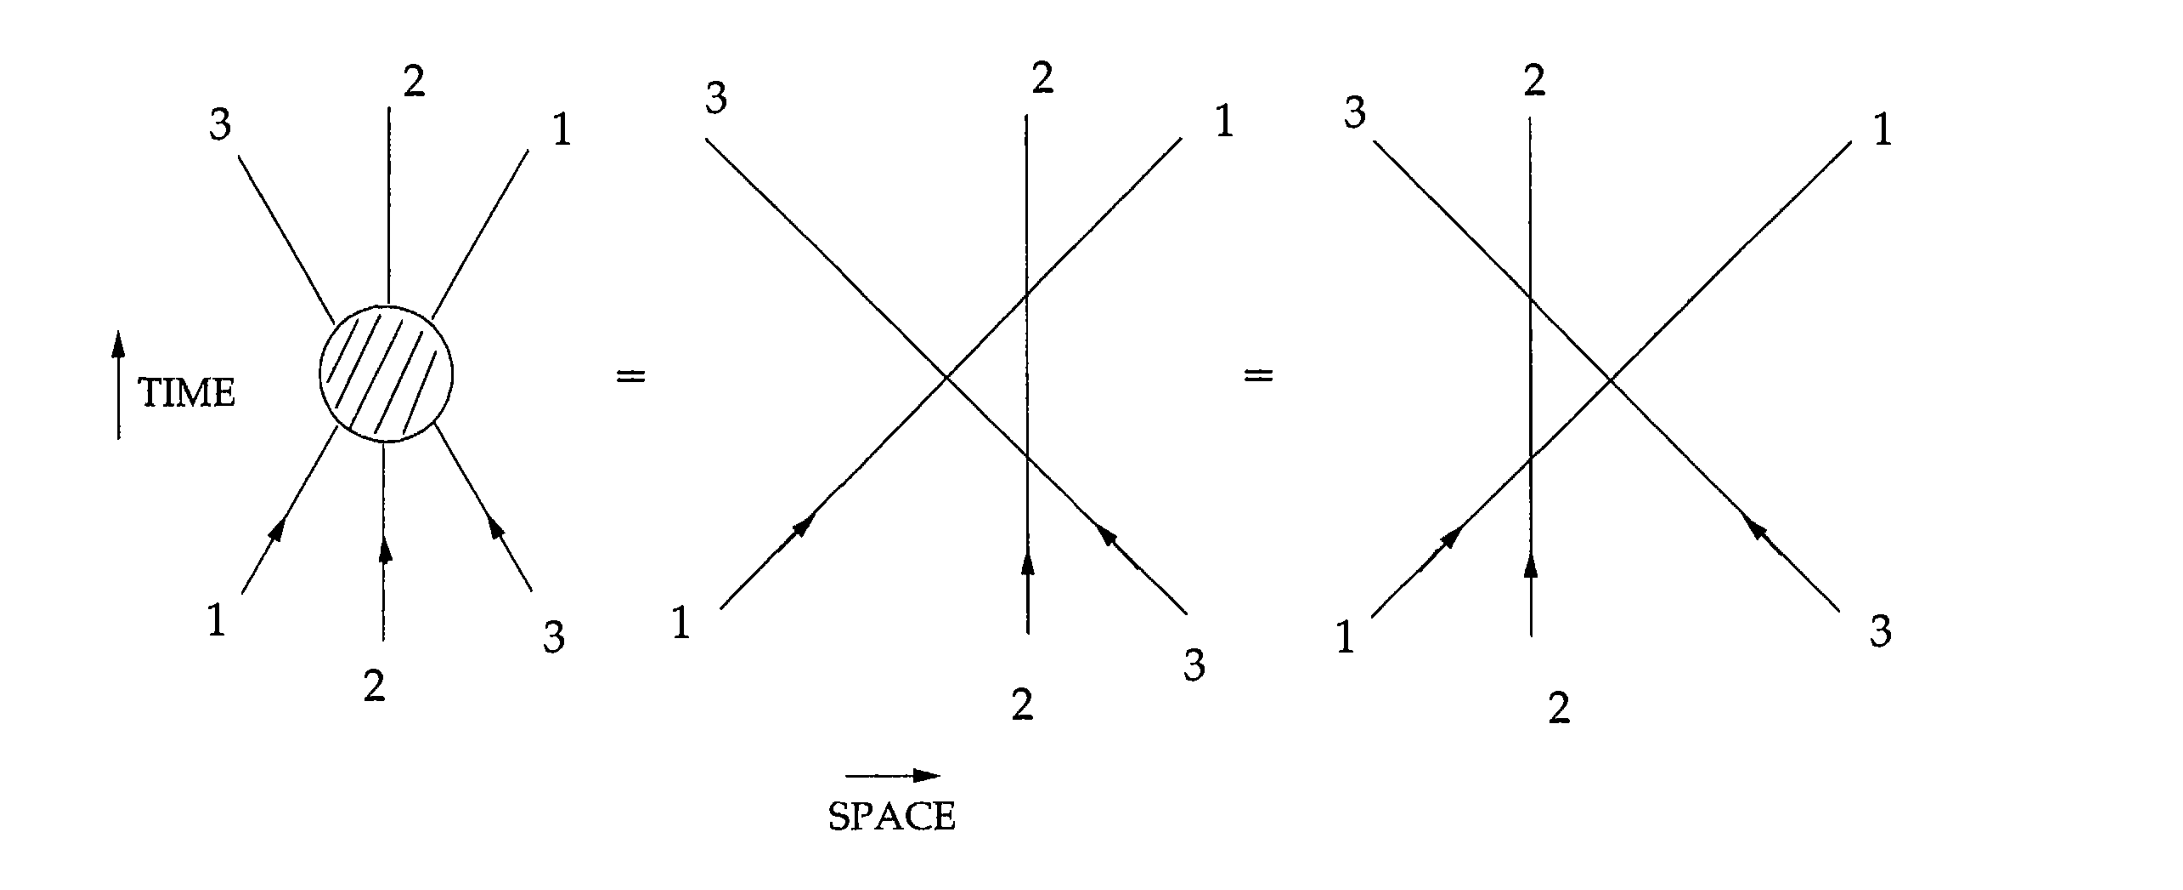
\includegraphics[width=0.78\textwidth]{figs/fig_p061_1.png}
  \caption{二维中三体散射约化为接连的三次两体碰撞。左：阴影圆盘表示一般的 $3\to3$ 散射；中、右：与它相等的两种图象，把该过程分解为三次 $2\to2$ 碰撞，两者的差别只在于这三次碰撞的先后次序（由「被禁戒」的对称性相联系）。纵轴为时间（TIME，向上），横轴为空间（SPACE，向右）；数字 $1,2,3$ 标记粒子，线上箭头指示动量方向。（原文 Figure 1，p.61；原图未给图号，此编号为本译本所加）}
  \label{fig:p061-1}
\end{figure}

然而在二维，两条直线一般是相交的，所以我们不能由上面的论证断定 $S$ 矩阵等于 $1$。不过，由于三条直线一般不会交于同一点，上面的论证表明：散射归结为（如图中所示）接连的三次两体碰撞，每一次都是两个粒子进、两个粒子出。这三次碰撞在时间次序上有两种可能，如图所示；而「被禁戒的」对称性意味着，对这两种时间次序，这三次碰撞相继发生的 $S$ 矩阵是相同的。

现在让我们回到靶空间为 $S^{N-1}$ 的 $\sigma$ 模型。在这个情形，如我们所知（对充分大的 $N$；并且我们相信对一切 $N>3$ 皆然），我们有 $N$ 个质量同为 $m$ 的有质量粒子，它们构成 $SO(N)$ 的一个 $N$ 维表示 $V$（即单粒子态空间是 $V\otimes L^2(\mathcal{O}_m^+)$）。上述论证允许我们对散射矩阵作出如下结论。

\subsection{映入 $S^{N-1}$ 的 $\sigma$ 模型的 $S$ 矩阵}

\noindent(i) $S$ 矩阵完全由「弹性两体散射（elastic two-body scattering）」决定，即由 $S$ 的两个入射、两个出射粒子的矩阵元决定。在这类散射中动量没有变化，所以 $S$ 矩阵约化成一个普通的矩阵值函数，即一个形如 $S(\lambda_1-\lambda_2)$、取值于 $\operatorname{End}_{SO(N)}(V\otimes V)$ 的函数，其中 $\lambda_i$ 由 $k_i=(me^{\lambda_i},me^{-\lambda_i})$ 定义，$k_i$ 是入射粒子的动量。（洛伦兹不变性意味着 $S$ 只依赖于差 $\lambda_1-\lambda_2$。）于是，$S$ 矩阵由如下形式的矩阵值函数显式描述：
\begin{equation}
  \tag{4.22}
  \label{eq:4-22}
  S(\theta)_{ij}^{kl}=F(\theta)\delta_i^k\delta_j^l+G(\theta)\delta_i^l\delta_j^k+H(\theta)\delta_{ij}\delta^{kl},
\end{equation}
其中 $F,G,H$ 是复值函数。

\noindent(ii) $S(\lambda)$ 满足量子 Yang–Baxter 方程：
\begin{equation}
  \tag{4.23}
  \label{eq:4-23}
  S_{12}(\lambda_1-\lambda_2)S_{13}(\lambda_1-\lambda_3)S_{23}(\lambda_2-\lambda_3)
  =S_{23}(\lambda_2-\lambda_3)S_{13}(\lambda_1-\lambda_3)S_{12}(\lambda_1-\lambda_2).
\end{equation}

\noindent(iii) 对任何实的 $\lambda$，$S(\lambda)$ 是幺正矩阵。

\noindent(iv) 交叉对称性（crossing symmetry）：$S$ 亚纯延拓到复平面，且
\[
S_{ij}^{kl}(\lambda)=S_{li}^{jk}(\pi i-\lambda).
\]

性质 (i) 我们基本上已经解释过；它就是「任何散射过程都由一串 $2\to2$ 过程决定，再加上 $SO(N)$ 对称性来约束 $2\to2$ 矩阵元」这一陈述。性质 (ii) 来自以下事实：$3\to3$ 散射矩阵分解为三个 $2\to2$ 散射
% ===== 原文 p.62 =====
矩阵之积，而这三次 $2\to2$ 碰撞发生的次序可以由图中的「被禁戒」对称性颠倒过来。性质 (iii) 对任何场论的 $S$ 矩阵都成立。性质 (iv) 称为交叉对称性，它是相对论场论的特征之一，在非相对论量子力学中没有对应物。粗略地说，它来自以下事实：$2\to2$ 的 $S$ 矩阵是四点函数极点的留数，而四点函数可以延拓到复的动量值。于是（由于庞加莱群的复化是连通的）$S$ 矩阵必须在庞加莱群的不连通分支下也不变，而该分支交换过去与未来，从而交换初态与末态粒子。（细节见去年秋季关于公理化的几讲。）

% [Tutor Note: 这里有一个容易读漏的指标结构，值得动手核一遍。把 (4.22) 看成 $V\otimes V$ 上的算子 $v^{ij}\mapsto S^{kl}_{ij}v^{ij}$，则它在三个不可约道上的本征值是：反对称道 $F-G$、对称无迹道 $F+G$、单态道 $F+G+NH$（后者的来历是 $\delta^{ij}\delta_{ij}=N$）。这个分解有两个用处：其一，可以立刻看出 (4.22) 的第三项必须写成 $\delta_{ij}\delta^{kl}$（两个下指标、两个上指标地配对），若写成 $\delta_i^j\delta^{kl}$ 之类则连指标类型都不对（多出一个上指标），$S$ 与 $SO(N)$ 对易这一条（即 (i) 中取值于 $\operatorname{End}_{SO(N)}(V\otimes V)$）也就无从谈起；其二，交叉对称性 $S^{kl}_{ij}(\lambda)=S^{jk}_{li}(\pi i-\lambda)$ 与 (4.22) 联立时，$F$ 项与 $F$ 项、$G$ 项与 $G$ 项、$H$ 项与 $H$ 项要各自配对，这正是 (4.24) 中三项之所以能共用一个标量因子 $f$ 的结构性原因。]

A. Zamolodchikov 与 Al. Zamolodchikov 于 1979 年证明：对 $N\ge3$，$S$ 矩阵被这些条件唯一确定，至多差一个依赖于 $\theta$ 的标量因子——前提是它非平凡（这一点我们可以从大 $N$ 展开得到）。在允许乘上一个对 $F,G,H$ 公共的标量函数 $f$ 的意义下，这个 $S$ 矩阵的 $F,G,H$ 由一个简单的显式公式给出：
\begin{equation}
  \tag{4.24}
  \label{eq:4-24}
  F(\theta)=1,\qquad G(\theta)=-\frac{2\pi i}{N-2}\,\theta,\qquad H(\theta)=-\frac{2\pi i}{(N-2)(\pi i-\theta)}.
\end{equation}

% [Tutor Note: 若把 (4.24) 当成完整的 $S$ 矩阵直接验证 (iii)（幺正性），会碰上一个真实的反例，值得记下来：取 $\theta=0$，则 $F=1$、$G=0$、$H(0)=-\frac{2\pi i}{(N-2)\pi i}=-\frac{2}{N-2}$；按上一条批注，(4.22) 的三个本征值是 $F-G=1$、$F+G=1$、$F+G+NH=1-\frac{2N}{N-2}$，最后一个对任何 $N>2$ 的模都不为 $1$（$N=3$ 时为 $-5$）。而 $f$ 对三项是公共因子，$\theta=0$ 时它只是一个数、只能把三个本征值同时缩放，故 $\{1,1\}$ 与 $1-\frac{2N}{N-2}$ 不可能被同时变成模 $1$——可见这不是「$f$ 尚未确定」造成的假象。因此 (4.24) 中分母 $N-2$ 值得核对：若换成 $N$，则 $H(0)=-2/N$，单态道本征值为 $1+NH(0)=1-2=-1$，于是 $\theta=0$ 处三个本征值 $\{1,1,-1\}$ 全在单位圆上，(iii) 立即成立。但 $N-2$ 在此处出现两次（$G$ 与 $H$），若真是排印之误应两处同改；稳妥的做法是把它记为原文存疑，对照 A. Zamolodchikov, Al. Zamolodchikov, Annals Phys.\ 120 (1979) 253 的原文核实后再定，不宜径改。另可注意 $H$ 在 $\theta=\pi i$ 处的极点正是交叉道的极点，这与 (iv) 中 $\pi i-\lambda$ 的平移互相印证，也说明 $(\pi i-\theta)$ 这个因子本身是对的。]

这个量子 Yang–Baxter 方程的解，是量子群（quantum group）理论据以发端的主要例子之一。与它相应的量子群现在称为「$\mathfrak{so}(N)$ 的 Yangian」（见 Drinfeld 在伯克利国际数学家大会上的报告「Quantum groups」）。

如我们已指出的，(4.24) 把 $S$ 矩阵确定到乘一个标量函数 $f(\theta)$ 为止。此外，这个函数满足条件
\[
f(\theta)f(-\theta)=1,\qquad f(\pi i-\theta)=f(\theta).
\]
因此 $f$ 是 $2\pi i$ 周期的。哪一个周期函数对应这个理论真正的 $S$ 矩阵，是一个不平凡的问题。微扰计算以及关于「简单性」的一般观念都强烈提示：这个函数应当这样选取，使得 $S$ 矩阵具有尽可能少的奇点。这样的选择有两个，其中之一被认为在 $\sigma$ 模型中实现；另一个选择被认为类似地在 Gross–Neveu 模型中实现。有趣的是，$f$ 不影响各反应的概率（因为对实的 $\lambda$ 它不影响 $F,G,H$ 的绝对值），但 $f$ 仍然重要，因为它影响散射过程中的「时间延迟」。

这样，我们就确定了映入 $S^{N-1}$ 的 $\sigma$ 模型的 $S$ 矩阵。人们也可以用这类论证确定该理论中算符在物理态之间的矩阵元（办法是写下 Yang–Baxter 方程的「表亲」方程，它们想必在量子群的语言中有其解释），但这一点我不打算讨论。

% [Tutor Note: 原文此处有一处排印重复：「One can show in a similar way the the Gross-Neveu model…」，多打了一个 the，应读作 the Gross–Neveu model。同一段还提到 Gross–Neveu 模型「用另一个极小的 $f$ 选择」得到其 $S$ 矩阵：这两个极小解分别对应 $\sigma$ 模型与 Gross–Neveu 模型，而它们在解析结构上的差别（极点分布不同）正是「$f$ 影响时间延迟却不影响概率」的具体体现——由于 $f$ 对 $F,G,H$ 是公共因子，各反应道之间的相对概率不变（这正是原文括号中那句话的稳妥读法），但散射的相移、从而时间延迟会改变。]

可以用类似方式证明：[I-Renorm Groups] 第 4 讲引入的 Gross–Neveu 模型同样是可积的，其意义与 $\sigma$ 模型相同。如我们已经提到的，它的 $S$ 矩阵是用另一个极小的 $f$ 选择得到的。

但映入球面的 $\sigma$ 模型与 Gross–Neveu 模型都是例外。在下一讲我们就会考虑一个稍复杂的 $\sigma$ 模型——靶空间为 $\mathbb{CP}^N$ 的模型，它不可积，其 $S$ 矩阵的显式形式未知，而且想必在某种意义上是无法知道的。

% ===== 原文 p.63 =====
在春季学期习题中有一个问题，要求证明以球面为靶空间的超对称 $\sigma$ 模型（supersymmetric sigma model）像它的玻色表亲一样可积。你还会在那个问题中看到：超对称 $\sigma$ 模型在某种意义上是普通 $\sigma$ 模型与 Gross–Neveu 模型的结合。顺便说一句，靶空间为 $\mathbb{CP}^N$ 的超对称模型也是可积的，尽管以该空间为靶空间的玻色 $\sigma$ 模型不可积。

\subsection{参考文献与交叉引用}

量子场论中散射的公理化在 [I-Axiomatics] 第 4 讲中讨论。二维 $\sigma$ 模型，特别是映入正曲率空间的二维 $\sigma$ 模型其 $\beta$ 函数为负这一事实，在 [II-CFT] 第 3 讲中讨论。Gross–Neveu 模型与本讲所讨论的非线性 $\sigma$ 模型密切相关，并有相似的 $1/N$ 展开，它在 [I-Renorm Groups] 第 4 讲中讨论。这些讲末尾的问题 3 与问题 4 涉及本文所述思想的超对称推广；问题 5 也涉及映入球面的 $\sigma$ 模型的大 $N$ 极限。

关于映入球面的 $\sigma$ 模型的高自旋守恒荷的构造，见
\begin{itemize}
  \item[] Y. Y. Goldschmidt, E. Witten, \textit{Conservation laws in some two-dimensional models}, Phys.\ Lett.\ \textbf{91B} (1980), 392.
\end{itemize}

关于 $\sigma$ 模型 $S$ 矩阵的计算，见
\begin{itemize}
  \item[] A. Zamolodchikov, Al. Zamolodchikov, \textit{Factorized $S$-matrices in two-dimensions as the exact solutions of certain relativistic quantum field models}, Annals Phys.\ \textbf{120} (1979), 253--291.
\end{itemize}

关于 Coleman–Mandula 定理在二维失效的直观讨论，以及若干精确 $S$ 矩阵的另外一些构造，见
\begin{itemize}
  \item[] R. Shankar, E. Witten, \textit{$S$ matrix of the supersymmetric nonlinear $\sigma$ model}, Phys.\ Rev.\ \textbf{D17} (1978), 2134.
\end{itemize}

% [Tutor Note: 文献条目按学术惯例保留原文（作者、篇名、卷号、页码），以便与原始文献对照；正文中的交叉引用代号 [I-Axiomatics]、[II-CFT]、[I-Renorm Groups] 分别指本丛书第 I 卷「公理化场论」、第 II 卷「共形场论」与第 I 卷「重整化群」的相应章节。注意 Goldschmidt–Witten 一文讨论的正是本讲 p.59 用数维度构造出的那个高自旋守恒荷（其自旋为 $3$），而 Shankar–Witten 一文给出的超对称非线性 $\sigma$ 模型 $S$ 矩阵是本讲 p.62 所说「两个极小 $f$ 选择」在超对称情形下的对应物。]


\clearpage
% 原文 pp.65–72（印刷 pp.1183–1190）
\section{Lecture 5：$\sigma$ 模型的大 $N$ 极限与 Grassmann 流形}

\begin{keytakeaways}
本讲研究映入复 Grassmann 流形 $\mathrm{Gr}(k,N)$（$\mathbb{C}^N$ 的 $k$ 维子空间构成的流形）及其实形式的二维 $\sigma$ 模型在大 $N$ 极限（$k$ 固定、$N\to\infty$）下的红外行为；由于 Grassmann 流形具有正 Ricci 曲率，这些理论是渐近自由的。核心数学工具是一整套「丛改写」：把映入弯曲靶空间的映射 $\phi$ 换成丛映射 $\phi^*s$，即把 $\phi^*S$ 替换为一个固定的秩 $k$、次数 $d$ 的 Hermite 向量丛 $E$，并引入等距嵌入 $\hat\phi:E\to\Sigma\times\mathbb{C}^N$（约束 $\hat\phi^*\hat\phi=\mathrm{id}_E$）与一个可变 $U(k)$ 联络 $A$。由此原来的非线性 $\sigma$ 模型 (5.1) 被改写为关于 $(\hat\phi,A,\sigma)$ 的等价作用量 (5.12)，其中 $\sigma$ 是施加约束的 Lagrange 乘子场；对 $\hat\phi$ 作 Gauss 积分后得到以 $\mathrm{Tr}\ln$ 表示的有效作用量 (5.13)，再取鞍点即得 $1/N$ 展开的主导阶。主要结论有三：其一，$\tilde\sigma$ 在红外获得动力学生成的质量 $M^2=\Lambda^2e^{-4\pi/\tilde g^2}$，故大 $N$ 极限存在质量间隙；其二，一圈计算表明 $\tilde\sigma$ 与 $A$ 都获得质量项（(5.16)、(5.19)），于是长距离行为等价于带 $\theta$ 项的二维 $U(k)$ 规范理论与带荷有质量标量的理论 (5.20)；其三，对实 Grassmann 流形，$\theta$ 项只能取 $0$ 或 $\pi$，且可写成无穷远处的 Wilson 圈算符 (5.22)——这一表述对任意连通紧 Lie 群都成立。
\end{keytakeaways}

% ===== 原文 p.65 =====
% 原文页首标题：LECTURE 5 / The Large $N$ Limit of the $\sigma$-model into Grassmannians
\noindent\textit{（本讲标题：映入 Grassmann 流形的 $\sigma$ 模型的大 $N$ 极限。）}

本讲我们讨论映入 Grassmann 流形 $\mathrm{Gr}(k,N)$ 的二维 $\sigma$ 模型的大 $N$ 行为，这里 $\mathrm{Gr}(k,N)$ 是 $\mathbb{C}^N$ 的 $k$ 维子空间所构成的 Grassmann 流形（Grassmannian）。其中 $k$ 固定，而 $N\to\infty$。我们也会考虑实 Grassmann 流形。由于 Grassmann 流形具有正 Ricci 曲率，这些场论是渐近自由（asymptotic freedom）的；但无论如何，我们的任务是研究其红外行为。

$\sigma$ 模型的欧氏作用量为
\begin{equation}
  \tag{5.1}
  \label{eq:5-1}
  S[\phi]=\frac{1}{g^2}\int_\Sigma d^2x\,|d\phi|^2-i\theta\int_\Sigma \phi^*(\alpha),
\end{equation}
其中 $\Sigma$ 是一个 Riemann 面（Riemann surface），$\phi:\Sigma\to\mathrm{Gr}(k,N)$ 是映入 Grassmann 流形的映射，$\alpha\in H^2(\mathrm{Gr}(k,N),\mathbb{Z})$ 是上同调的一个生成元，$g$、$\theta$ 是理论的参数。我们马上就会指定 $\mathrm{Gr}(k,N)$ 上的度量。第二项是拓扑项；当 $\Sigma$ 闭时，该积分取整数值。因此 $\theta\to\theta+2\pi$ 的移动不影响模型。$\theta$ 也是量子理论的参数，但重整化会把无量纲的耦合常数 $g$ 换成一个质量参数 $\mu$。

由
\begin{equation}
  \tag{5.2}
  \label{eq:5-2}
  g^2=\tilde{g}^2/N
\end{equation}
定义的重标度耦合常数 $\tilde{g}$，在大 $N$ 极限下更为自然，这一点我们将会看到。

% [Tutor Note: (5.1) 中拓扑项写成 $i\theta\int_\Sigma\phi^*(\alpha)$，其周期 $\theta\sim\theta+2\pi$ 依赖 $\alpha$ 是 $H^2(\mathrm{Gr}(k,N),\mathbb{Z})$ 的整系数生成元（即 $\int_\Sigma\phi^*\alpha\in\mathbb{Z}$）。若把 $\alpha$ 换成 $m\alpha$（$m>1$）或换用有理系数类，$\theta$ 的周期就变成 $2\pi/m$，全部 $\theta$ 依赖的表达式都会随之改变。另外，欧氏作用量中的因子 $i$ 并非笔误：它使 $S$ 在定向反转下取复共轭（$\phi^*\alpha$ 变号），从而延拓到 Minkowski 空间后作用量是实的——这正是脚注 11 的意思。]

\subsection*{§5.1　问题}
% 原文 §5.1：The questions

我们针对模型的行为提出几个具体问题。

\begin{enumerate}
  \item 是否存在质量间隙（mass gap）？
  \item 配分函数对 $\theta$ 的依赖是什么？
\end{enumerate}

\noindent\textbf{注（Remark）.} 当 $\Sigma$ 很小时，配分函数
\[
  Z(\theta)=\int D\phi\,\exp\left(-\frac{1}{g_{\mathrm{eff}}^2}\int_\Sigma d^2x\,|d\phi|^2+i\theta\int_\Sigma\phi^*(\alpha)\right)
\]
可以用微扰论来研究。这里 $g_{\mathrm{eff}}$ 是有效耦合（effective coupling），它随理论中由 $\Sigma$ 的大小所设定的距离标度而变化。（经典地看模型是共形不变的，因此不依赖 $\Sigma$ 的大小；但量子力学地看这已不再成立。）由渐近自由，该耦合在小距离处很小，于是才有「微扰论适用于这一区域」的论断。

\noindent\textit{（本讲笔记由 Daniel Freed 整理。）}

% ===== 原文 p.66 =====
现在，(5.1) 的经典解是调和映射（harmonic map）$\Sigma\to\mathrm{Gr}(k,N)$。注意 $\theta$ 依赖只通过对 $\phi$ 的度（degree）出现，因此我们把积分按映射 $\phi$ 的度分解为求和。在度 $0$ 我们得到常数映射；一般地，在度 $n$ 得到调和映射的某个模空间 $\mathcal{M}_n$，它们就是本模型的瞬子（instanton）。度 $1$ 的瞬子是（反）全纯映射。围绕这些解的微扰展开大致具有如下形式：
\begin{equation}
  \tag{5.3}
  \label{eq:5-3}
  Z(\theta)\sim\frac{\operatorname{Vol}(\mathrm{Gr}(k,N))}{\sqrt{\det(\cdot)}}\,(1+\cdots)
  +\sum_{\pm}e^{\pm i\theta}e^{-cN/g_{\mathrm{eff}}^2}\frac{\operatorname{Vol}\mathcal{M}_1}{\sqrt{\det(\cdot)}}\,(1+\cdots)
  +\text{更高的瞬子}.
\end{equation}

指数上的常数 $c$ 是一个 1-瞬子的作用量，它与 $N$ 无关。因子 $N$ 则来自 (5.2)。若 $g_{\mathrm{eff}}\ll1$，我们看到 $Z(\theta)$ 中依赖 $\theta$ 的项当 $N\to\infty$ 时指数式地消失。随着 $\Sigma$ 的面积增大，有效耦合 $g_{\mathrm{eff}}$ 也随之增大。方程 (5.3) 是 $\Sigma$ 紧致且面积很小时的答案；但对 $\Sigma=\mathbb{R}^2$ 我们将得到一个极不相同的结论。

% [Tutor Note: (5.3) 中每一项都写成「体积因子 / $\sqrt{\det(\cdot)}$」，这个比值才是真正有意义的量：分子是相应模空间（度 $0$ 时即靶空间 $\mathrm{Gr}(k,N)$ 本身，度 $1$ 时是瞬子模空间 $\mathcal{M}_1$）的体积，分母是围绕该经典解展开所得的自由涨落算符的行列式平方根。两个因子各自都依赖截断与度规，只有比值在重整化后有意义；这也解释了为什么度 $0$ 项（常数映射）不带 $\theta$ 因子——常数映射的度为零，$\int\phi^*\alpha=0$。]

\noindent\textbf{3. 对称性破缺（Symmetry Breaking）.} 在二维，对称性破缺只对离散对称性才可能发生，而本模型中我们有宇称对称性（parity symmetry）
\begin{equation}
  \tag{5.4}
  \label{eq:5-4}
  \begin{aligned}
    P:\;&\Sigma\longmapsto\bar\Sigma\qquad(\bar\Sigma\ \text{是取相反定向的}\ \Sigma)\\
    &\theta\longmapsto-\theta
  \end{aligned}
\end{equation}

对 $\Sigma=\mathbb{R}^2$，我们用一个反转定向的等距变换（isometry），即一次反射，来实现定向反转。于是对 $\theta=0$ 与 $\theta=\pi$，宇称 $P$ 作用于一个固定的理论，我们问它在量子理论中是否破缺。

% [Tutor Note: 值得指出，使 (5.4) 成为对称性的并不是单靠 $\theta\to-\theta$，而是「定向反转 $\Sigma\to\bar\Sigma$ 与 $\theta\to-\theta$ 的联合」。因此在 $\theta$ 的 $2\pi$ 周期性下，只有 $\theta=0$ 与 $\theta=\pi$（后者因 $-\pi\equiv\pi \bmod 2\pi$ 而自共轭）才是 $P$ 的不动点，这也正是作者只讨论这两个值的理由；$\theta=\pi$ 处若 $P$ 自发破缺，就会出现两条简并的真空。]

\noindent\textbf{4.} Grassmann 流形的等距群 $PSU(N)$ 在经典理论中有作用。由于连续对称群在二维不会破缺，这个对称性在量子理论中同样有作用。然而，理论的一个实现（realization）所带的对称群有可能是 $PSU(N)$ 的覆盖群，而 $PSU(N)$ 本身才是作用于算符代数上的群。这里会发生这种情况吗？

\subsection*{§5.2　一个等价的表述}
% 原文 §5.2：An equivalent formulation

为了研究这个模型，我们把它改写，也就是说，我们构造一个具有相同经典与量子物理的作用量。作为准备，我们先回忆 Grassmann 流形的一些基本几何。在 $\mathrm{Gr}(k,N)$ 之上有一个典范的向量丛正合列
\begin{equation}
  \tag{5.5}
  \label{eq:5-5}
  0\longrightarrow S\xrightarrow{\ s\ }\mathrm{Gr}(k,N)\times\mathbb{C}^N\longrightarrow Q\longrightarrow 0,
\end{equation}
其中 $S$ 在 $k$ 维平面 $\pi$ 处的纤维就是看作 $\mathbb{C}^N$ 子空间的 $\pi$ 本身。固定 $\mathbb{C}^N$ 上的标准度量。它在 $S$ 上诱导一个度量，并给出同构 $Q\cong S^\perp$。在 $S$ 上存在

% ===== 原文 p.67 =====
一个典范联络（canonical connection）$\nabla$，它由平凡丛 $\mathrm{Gr}(k,N)\times\mathbb{C}^N$ 上的自然联络投影而来。我们容易算出
\begin{equation}
  \tag{5.6}
  \label{eq:5-6}
  \nabla=d-s^*ds,
\end{equation}
其中 $s$ 是包含映射 $S\xrightarrow{\ s\ }\mathrm{Gr}(k,N)\times\mathbb{C}^N$。于是
\begin{equation}
  \tag{5.7}
  \label{eq:5-7}
  \nabla s:\ T\bigl(\mathrm{Gr}(k,N)\bigr)\longrightarrow\operatorname{Hom}(S,S^\perp)
\end{equation}
是一个同构。我们用它来在 $\mathrm{Gr}(k,N)$ 上诱导一个度量，这正是写下 $\sigma$ 模型作用量 (5.1) 所需要的度量。

现在设 $\phi:\Sigma\to\mathrm{Gr}(k,N)$。我们把 (5.5) 拉回到 $\Sigma$ 上，得到 $\Sigma$ 上的一列丛；再由 (5.7)，$\phi$ 的拉格朗日密度为
\begin{equation}
  \tag{5.8}
  \label{eq:5-8}
  |d\phi|^2=|(\phi^*\nabla)\phi^*s|^2 .
\end{equation}

注意 $\phi^*s:\phi^*S\to\Sigma\times\mathbb{C}^N$ 决定了 $\phi$。这里的想法是把 $\phi$ 换成这样一个丛映射，因而首先要做的就是把 $\phi^*S$ 换成一个固定的丛。注意 $\deg(\phi^*S)=\deg(\phi)$，所以 $\phi^*S$ 的拓扑决定了上同调类 $\phi^*(\alpha)$，而后者出现在作用量 (5.1) 的第二项中。于是固定一个秩为 $k$、次数为 $d$ 的向量丛 $E\to\Sigma$。再固定 $E$ 上的一个 Hermite 度量。我们引入一个新场
\[
  \hat\phi:\ E\longrightarrow\Sigma\times\mathbb{C}^N,
\]
并约束它是一个等距浸入（isometric immersion）：
\begin{equation}
  \tag{5.9}
  \label{eq:5-9}
  \hat\phi^*\hat\phi=\mathrm{id}_E .
\end{equation}

$\hat\phi$ 的像决定了一个映射 $\phi:\Sigma\to\mathrm{Gr}(k,N)$；若把 $\hat\phi$ 作 $E$ 的一次酉规范变换，该映射不变。为了用 $\hat\phi$ 改写 (5.8)，我们需要 $E$ 上的一个联络，而既然没有自然的选择，我们就引入一个可变的酉联络 $A$。借助 $\hat\phi$，我们把 $E$ 等同于平凡丛 $\Sigma\times\mathbb{C}^N$ 的一个子丛，于是可以用通常的导数 $d$ 来微分 $\hat\phi$。把 $A$ 写成一个 1-形式加上这个平凡联络，我们得到
\begin{equation}
  \tag{5.10}
  \label{eq:5-10}
  \begin{aligned}
    |d_A\hat\phi|^2&=|d\hat\phi+\hat\phi A|^2\\
    &=|d\hat\phi|^2+2\Re\,(d\hat\phi,\hat\phi A)+|A|^2,
  \end{aligned}
\end{equation}
这里用到了 $\hat\phi^*\hat\phi=\mathrm{id}_E$。这个表达式对 $A$ 是二次的，因此若把 (5.10) 看作 $A$ 的经典拉格朗日量，我们就可以用运动方程得到
\begin{equation}
  \tag{5.11}
  \label{eq:5-11}
  A_0=-\hat\phi^*d\hat\phi .
\end{equation}
与 (5.6) 比较可见，$A_0$ 正是 $S$ 上典范联络的拉回，于是由 (5.8)
\[
  |d\phi|^2=|d_{A_0}\hat\phi|^2 .
\]
换言之，对满足约束 (5.9) 的场，(5.10) 这个拉格朗日量等价于 $|d\phi|^2$。我们通过一个 Lagrange 乘子场来施加该约束：
\[
  \sigma:\ \Sigma\longrightarrow\operatorname{HermitianEnd}(E).
\]

% [Tutor Note: (5.10) 的第二行末尾只写了 $|A|^2$ 而不写 $|\hat\phi A|^2$，看似漏了 $\hat\phi$，其实正是用了约束 (5.9)：$|\hat\phi A|^2=\operatorname{Tr}\bigl[(\hat\phi A)^*(\hat\phi A)\bigr]=\operatorname{Tr}\bigl[A^*\hat\phi^*\hat\phi A\bigr]=|A|^2$。若忘了这条约束，就会错误地保留一个 $\hat\phi$ 依赖，从而得不到 (5.11) 这一干净的线性方程。]

% [Tutor Note: (5.11) 的符号完全取决于 $A$ 取反 Hermite（skew-Hermitian）这一约定，即 $d_A=d+A$ 而 $A^*=-A$。若改用物理文献常见的 Hermite 联络（$d_A=d-iA$，$A$ 为 Hermite 矩阵），则 (5.10) 的交叉项变号，驻点条件相应变成 $A_0=+\hat\phi^*d\hat\phi$（可能再带一个 $i$ 因子），而 (5.12) 中 $\operatorname{Tr}F_A$ 前的系数也要跟着调整。此处符号若抄错，后面 $A$ 与 $\hat\phi$ 的顶点费曼规则 (5.17) 之前的 $I=-i(k_1-k_2)_\mu$ 就会整体反号。]

% ===== 原文 p.68 =====
原作用量 (5.1) 中的 $\theta$ 项可以用（反 Hermite 的）曲率 $F_A$ 通过 Chern–Weil 理论算出。合起来，我们为新作用量得到\footnote{关于 Lagrange 乘子项，这里应当作一些说明。它基于一般公式
\[
  \int e^{i(\sigma,x)}\,d\sigma=\delta(x),
\]
其中 $\sigma$ 位于 $x$ 的对偶空间，测度 $d\sigma$ 取适当的归一化，$\delta(x)$ 是支撑在原点的 $\delta$ 分布。在 Minkowski 空间拉格朗日量中，Lagrange 乘子项是
\[
  \int_\Sigma\operatorname{Tr}\sigma\bigl(\hat\phi^*\hat\phi-\mathrm{id}_E\bigr),
\]
而 $\sigma$ 应被理解为二次形式（或密度）；它位于 $\hat\phi^*\hat\phi-\mathrm{id}_E$ 所在函数空间的对偶空间中。转动到欧氏空间即得 (5.12) 的第二项。当然，我们也可以直接在欧氏空间中引入 Lagrange 乘子项，理由完全相同。}
\begin{equation}
  \tag{5.12}
  \label{eq:5-12}
  S[\hat\phi,A,\sigma]=\frac{1}{g^2}\int_\Sigma|d_A\hat\phi|^2-i\int_\Sigma\operatorname{Tr}\sigma\bigl(\hat\phi^*\hat\phi-\mathrm{id}_E\bigr)+\frac{\theta}{2\pi}\int_\Sigma\operatorname{Tr}F_A .
\end{equation}

如我们已经解释的，由 (5.12) 算出的经典运动方程（以及其他经典构造）与由原作用量 (5.1) 算出的等价。导致 (5.11) 的那一步经典计算在量子层面同样有效，因为 (5.12) 对 $A$ 的依赖是二次的，且其 Hessian 就是恒等算符（见 (5.10)）。（我们忽略了从 $A$ 积分中得到的常数行列式因子。）因此量子物理也是相同的。

% [Tutor Note: 「对 $A$ 的依赖是二次的且 Hessian 是恒等算符」这句话是 (5.12) 与 (5.1) 量子等价的关键：对 $A$ 作 Gauss 积分只产生一个与场无关的常数行列式（作者随即略去），所以经典地消去 $A$ 与量子地消去 $A$ 给出同一个关于 $\hat\phi$ 的理论。反之，若 $A$ 的动能项 $\frac{1}{g^2}|F_A|^2$ 一开始就存在（如 (5.20) 那样），$A$ 的积分将不再平凡，这正是大 $N$ 下 $A$ 获得动力学项 (5.19) 的物理内容。]

\subsection*{§5.3　大 $N$ 有效理论}
% 原文 §5.3：The large $N$ effective theory

这里的论证与映入球面的大 $N$ $\sigma$ 模型（见第 4 讲）几乎完全相同，所以我们从简。

首先，$\hat\phi$ 积分是 Gauss 型的，因此配分函数为
\begin{equation}
  \tag{5.13}
  \label{eq:5-13}
  \begin{aligned}
    Z&=\sum_E\int\frac{DA}{\mathrm{vol}}\,D\sigma\,D\hat\phi\ e^{-S[\hat\phi,A,\sigma]}\\
    &=\sum_E\int\frac{DA}{\mathrm{vol}}\,D\sigma\,\exp-\left[\operatorname{Tr}\ln\left(\frac{d_A^*d_A}{g^2}-i\sigma\right)+i\int_\Sigma\operatorname{Tr}\sigma+\frac{\theta}{2\pi}\int_\Sigma\operatorname{Tr}F_A\right].
  \end{aligned}
\end{equation}

这里 $\sum_E$ 是对丛 $E$ 求和。我们取 $\Sigma=\mathbb{R}^2$。此时对 $E$ 的求和无关紧要，拓扑项也一样。作为对这一问题的第一步处理，丛的拓扑并不重要，因为它被摊开在一个无穷大的体积上。一旦我们对量子真空的样子有了基本了解，再回过头去看拓扑如何进入并不困难。和上周一样，我们通过在被积函数指数的驻点（即有效作用量的一个经典解）处取值，来求大 $N$ 下的主导行为。

规范场唯一可能的 Poincaré 不变（也就是欧氏不变）取法是 $A=0$。\footnote{曲率 $F=dA$ 若有非零的常数期望值，就不会在空间反射下不变——空间反射是 Euclid 群的连通分支之外的部分。对 $\theta\neq0$（它破坏反射对称性），我们最终会发现 $F$ 确实有非零的平均值，但它太小，不影响大 $N$ 的鞍点。} 因此自然地去找一个 $A=0$ 的驻点。

% [Tutor Note: (5.13) 中 $\operatorname{Tr}\ln$ 前的因子 $N$ 并非显式写出，而是在下一行（p.69）出现的，其来源是：$\hat\phi$ 是 $E^*\otimes\mathbb{C}^N$ 的截面，对 $\hat\phi$ 作 Gauss 积分给出 $\det(\cdot)^{-N}$，其中指数 $N$ 来自平凡因子 $\mathbb{C}^N$ 的维数，而 $\det$ 只作用在 $E^*$ 的截面上（所以 (5.12) 里 $\operatorname{Tr}$ 是对 $E$ 的 $k$ 维纤维取的）。若误以为 $\hat\phi$ 只有一个分量，就会漏掉这个 $N$，整个 $1/N$ 展开便无从谈起。]

% ===== 原文 p.69 =====
在那种情形下，我们把 (5.13) 最后一行的被积函数取负号后改写为
\[
  S_{\mathrm{eff}}[A,\sigma]=N\operatorname{Tr}\ln\left(\frac{d_A^*d_A}{g^2}-i\sigma\right)+i\int\operatorname{Tr}\sigma,
\]
其中第一项的算符作用在 $E^*$ 的截面上。现在唯一 Poincaré 不变的取法是 $\sigma$ 为常数，于是我们把 $\sigma$ 对角化，化为 $k$ 个关于单个本征值的一维问题。此时我们作重标度
\begin{equation}
  \tag{5.14}
  \label{eq:5-14}
  \begin{aligned}
    \sigma&=N\tilde\sigma,\\
    g^2&=\tilde{g}^2/N,
  \end{aligned}
\end{equation}
于是对每个本征值，我们面对的问题恰好就是映入球面的大 $N$ $\sigma$ 模型的问题。因此解 $\tilde\sigma_0$ 的所有本征值都相等，并由
\[
  -i\tilde{g}^2\tilde\sigma_0=\Lambda^2e^{-4\pi/\tilde{g}^2}=M^2
\]
确定，其中 $\Lambda$ 是紫外截断，而 $\tilde{g}^2$ 现在是跑动耦合常数。我们定义 $M^2$ 为这个动力学生成的质量平方。

% [Tutor Note: (5.14) 的两条重标度必须同时进行：$\sigma=N\tilde\sigma$ 使 $N\operatorname{Tr}\ln$ 与 $i\int\operatorname{Tr}\sigma$ 同阶（否则鞍点方程里 $N$ 的幂次不匹配），而 $g^2=\tilde{g}^2/N$ 使 $\frac{d_A^*d_A}{g^2}$ 与 $\sigma$ 同阶。只做其中一个，就会得到 $\tilde\sigma_0\sim N$ 或 $\tilde\sigma_0\sim1/N$ 的错误标度。也要注意这里出现的是 $\tilde g^2$ 而非 $g^2$：指数 $4\pi/\tilde g^2$ 与第 4 讲球面情形中 $2\pi/\tilde\lambda$ 的形式一致（那里 $\lambda$ 对应这里的 $\tilde g^2/2$ 一类的归一化），差别只是耦合的归一化约定。]

于是在大 $N$ 有效作用量中 $\tilde\sigma$ 获得了质量。注意 $A$ 场没有横向自由度——它是二维的规范场——因此并不扩大模型的谱（当然，正如我们将看到的，它影响 Hamiltonian，事实上还削减了谱）。所以大 $N$ 极限存在质量间隙。这就是我们问题清单中第一个问题的答案。

为了回答其余问题，我们需要算得更精确一些，即算出大 $N$ 有效作用量的领头近似。这意味着对作用量 (5.12) 在点 $\hat\phi_0=0$、$A_0=0$、$\tilde\sigma_0=iM^2/\tilde{g}^2$ 附近作微扰论。于是，把 $\tilde\sigma$ 平移 $\tilde\sigma_0$ 并对 $\hat\phi$ 重标度，由 (5.12) 我们得到
\begin{equation}
  \tag{5.15}
  \label{eq:5-15}
  S'[\hat\phi,A,\tilde\sigma]=\int_\Sigma|d_A\hat\phi|^2+M^2\int_\Sigma|\hat\phi|^2-i\tilde{g}^2\int_\Sigma\operatorname{Tr}\tilde\sigma\hat\phi^*\hat\phi+\frac{\theta}{2\pi}\int_\Sigma\operatorname{Tr}F_A .
\end{equation}

这里我们省略了一个常数项（它只把配分函数平移一个常数）以及 $\tilde\sigma$ 的一个线性项（因为我们是在有效作用量的一个解附近展开）。

\begin{figure}[htbp]
  \centering
  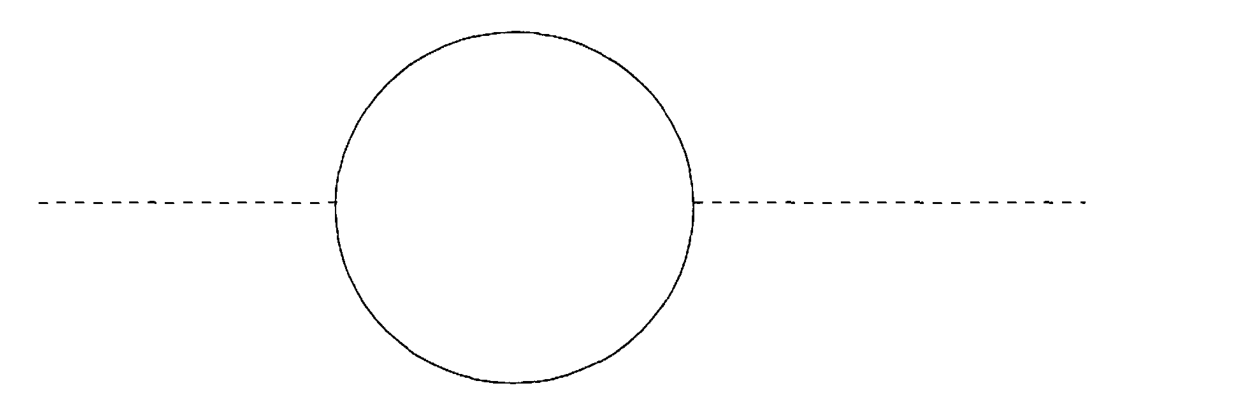
\includegraphics[width=0.55\textwidth]{figs/fig_p069_1.png}
  \caption{$\tilde\sigma$ 的逆传播子。（原文 Figure 5.1，p.69）图中实线圆环代表 $\hat\phi$ 圈，两侧虚线代表外部的 $\sigma$ 线。}
  \label{fig:p069-1}
\end{figure}

有效作用量是用单粒子不可约（one particle irreducible）Feynman 图在微扰论中算出的，其外线对应 $A$ 与 $\sigma$，内线对应 $\hat\phi$。因此 $\tilde\sigma$ 的逆传播子由

% ===== 原文 p.70 =====
Figure 5.1 所示的图算出，其中实线代表 $\hat\phi$，虚线代表 $\sigma$。（注意 (5.15) 中没有 $\tilde\sigma$ 的二次项，否则 Figure 5.1 就会是对这样一个二次项的修正。）我们在动量空间中把这个图算作
\begin{equation}
  \tag{5.16}
  \label{eq:5-16}
  \begin{aligned}
    -\tilde{g}^4Nk\int\frac{d^2q}{(2\pi)^2}\,&\frac{1}{q^2+M^2}\,\frac{1}{(p-q)^2+M^2}\\
    &=-\frac{\tilde{g}^4Nk}{4\pi^2}\int_0^1 d\alpha\int d^2q\,\frac{1}{\bigl[q^2+(M^2+\alpha(1-\alpha)p^2)\bigr]^2}\\
    &=-\frac{\tilde{g}^4Nk}{\pi}\int_0^1\frac{d\alpha}{M^2+\alpha(1-\alpha)p^2}\\
    &=-\frac{\tilde{g}^4Nk}{\pi M^2}+O(p^2)\qquad\text{当 }p\to0 .
  \end{aligned}
\end{equation}

这对应于有效作用量中的一项
\[
  C|\tilde\sigma|^2,
\]
其中 $C>0$。（负号之所以出现，是因为在欧氏理论中图给出的是对有效作用量的负贡献。）这是红外中的主导项，它意味着 $\tilde\sigma$ 是有质量的，因而不影响理论的长程行为。

% [Tutor Note: (5.16) 中 $Nk$ 的来源值得交代清楚：$\hat\phi$ 圈同时在两个「内部指标」上求迹——一重是平凡因子 $\mathbb{C}^N$（给出 $N$），一重是秩 $k$ 的丛 $E^*$（给出 $k$）；而两个 $\tilde\sigma\hat\phi^*\hat\phi$ 顶点各贡献一个 $-i\tilde g^2$，乘积给出 $-\tilde g^4$。这与 (5.13) 中 $\operatorname{Tr}\ln$ 前出现 $N$、迹取在 $E^*$ 上完全一致。]

% [Tutor Note: 对 (5.16) 的第二行到第三行存疑：由 2 维公式 $\int d^2q\,[q^2+\Delta]^{-2}=\pi/\Delta$，第二行给出 $-\tilde g^4Nk/(4\pi\Delta)$，而书中第三行写的是 $-\tilde g^4Nk/(\pi\Delta)$，两者相差因子 $4$；末行 $-\tilde g^4Nk/(\pi M^2)$ 与第三行自洽，可见四处必有一处笔误（或第二行分母本应为 $16\pi^2$）。作者用的是 Feynman 参数化 $\frac{1}{AB}=\int_0^1d\alpha\,[\alpha A+(1-\alpha)B]^{-2}$ 并平移 $q\to q-\alpha p$（平移后交叉项消失，$\Delta=M^2+\alpha(1-\alpha)p^2$）。这一数值系数只影响 $C$ 的大小，不影响「$\tilde\sigma$ 有质量、长程行为不受影响」的结论。]

\begin{figure}[htbp]
  \centering
  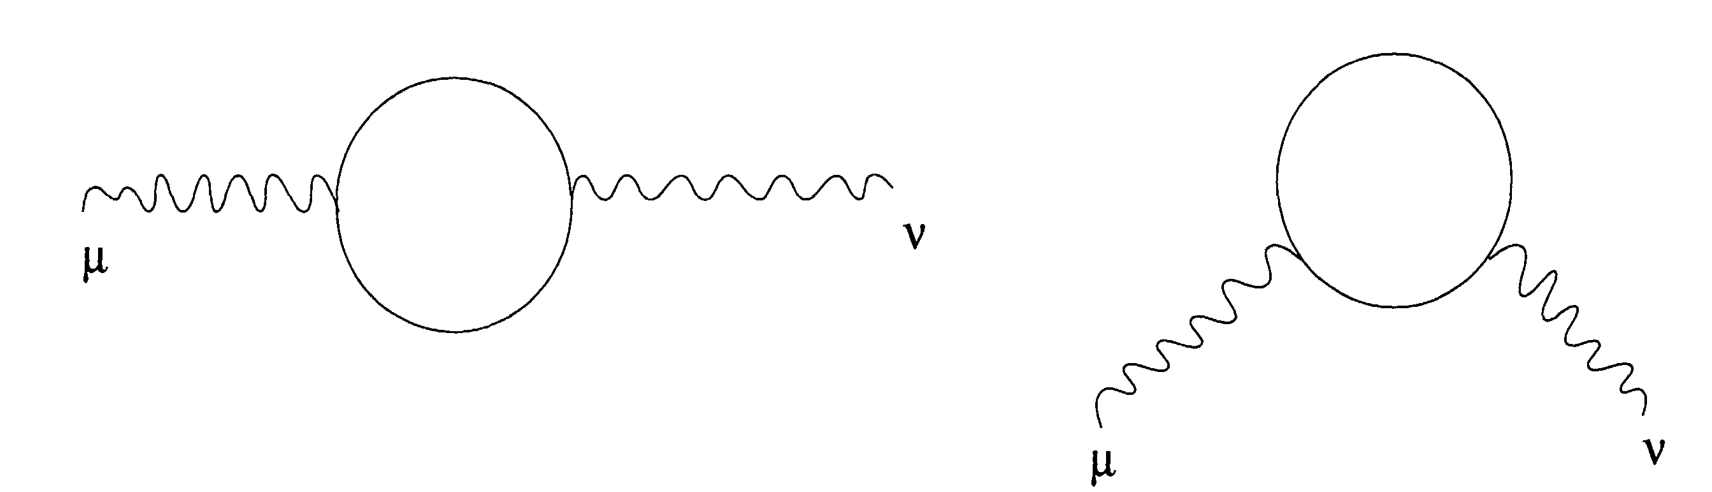
\includegraphics[width=0.85\textwidth]{figs/fig_p070_1.png}
  \caption{$A$ 的逆传播子。（原文 Figure 5.2，p.70）波浪线代表规范场 $A$，圆环为 $\hat\phi$ 圈，外线标有指标 $\mu,\nu$；左图由两个三顶点构成，右图为四顶点（蝌蚪型）图。}
  \label{fig:p070-1}
\end{figure}

\begin{figure}[htbp]
  \centering
  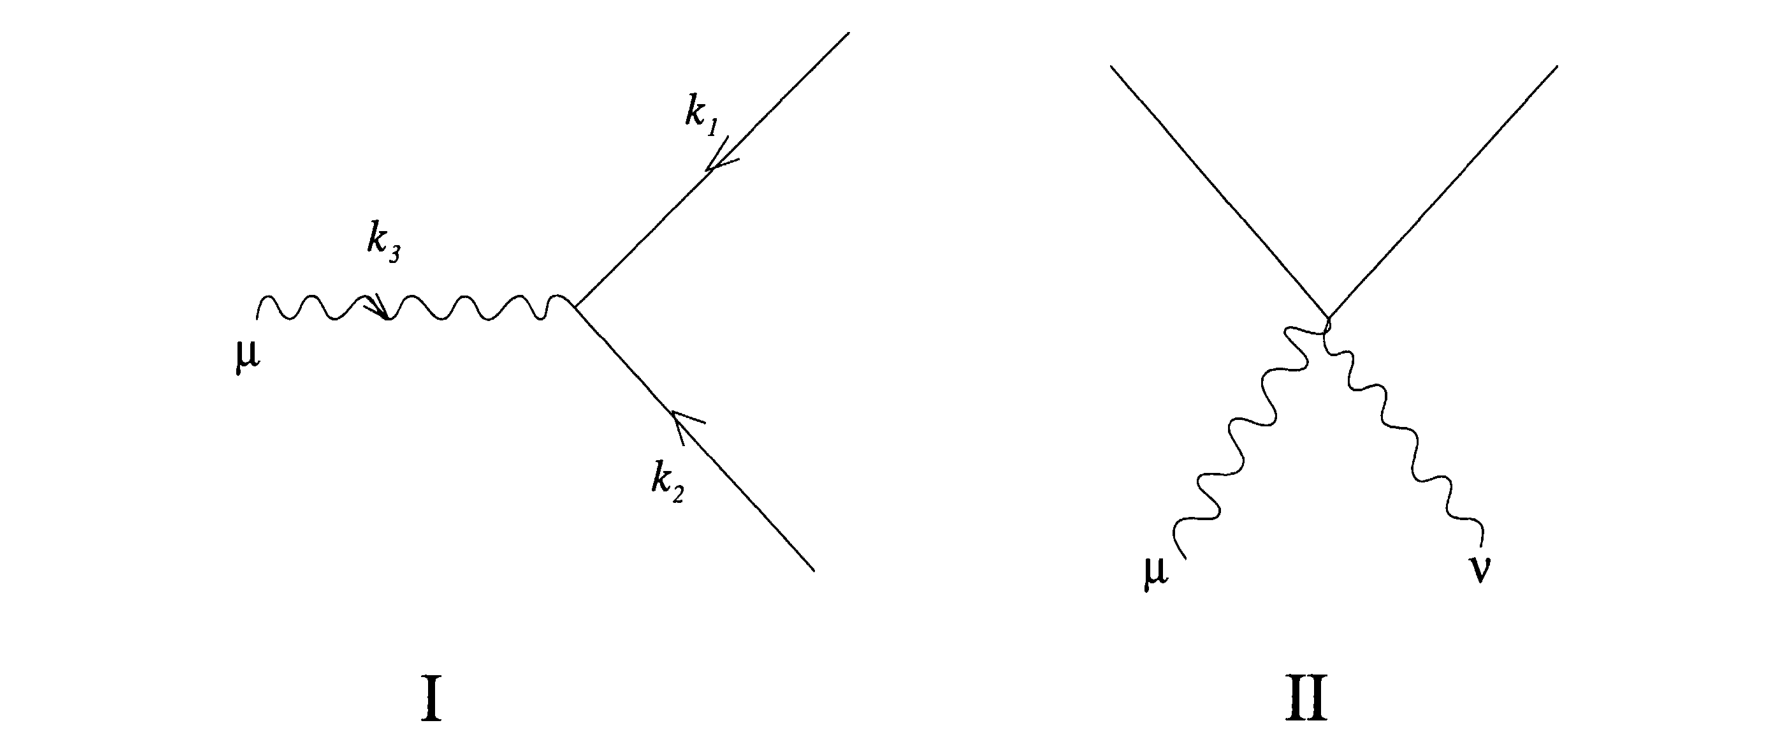
\includegraphics[width=0.85\textwidth]{figs/fig_p070_2.png}
  \caption{$A$ 场的相互作用顶点。（原文 Figure 5.3，p.70）图 I 为三顶点（入射动量 $k_1,k_2$，$A$ 线动量为 $k_3$，指标 $\mu$），图 II 为四顶点（指标 $\mu,\nu$）。}
  \label{fig:p070-2}
\end{figure}

% ===== 原文 p.71 =====
$A$ 的逆传播子由 Figure 5.2 中的图算出，它们来自 (5.15) 的第一项。这里波浪线代表 $A$。为计算这些图，我们需要 Figure 5.3 所示顶点的 Feynman 规则，这些顶点对应于作用量 (5.15) 中的项
\[
  2\Re\,(d\hat\phi,\hat\phi A)
\]
\[
  |\hat\phi A|^2 .
\]
其中的指标是相对于 $\mathbb{R}^2$ 的一组标准正交基而言的。第二个顶点的 Feynman 规则（在动量空间中）很简单：
\[
  II=-\delta_{\mu\nu}.
\]
（这里有一个负号，因为欧氏泛函积分含有 $e^{-S}$。）对顶点 $I$，我们必须记住 $\hat\phi$ 是复的，而 $A$ 是反 Hermite 的：
\[
  2\Re\,(\partial_\mu\hat\phi,\hat\phi A_\mu)=-\partial_\mu\hat\phi\,A_\mu\hat\phi^*+\hat\phi A_\mu\,\partial_\mu\hat\phi^* .
\]
于是该顶点为
\[
  I=-i(k_1-k_2)_\mu .
\]
注意顶点中两条实线之一代表 $\hat\phi$，另一条代表 $\hat\phi^*$。因此 Figure 5.2 中各图之和为
\begin{equation}
  \tag{5.17}
  \label{eq:5-17}
  \int\frac{d^2q}{(2\pi)^2}\frac{(p-2q)_\mu(p-2q)_\nu}{(q^2+M^2)\bigl((p-q)^2+M^2\bigr)}
  -2\delta_{\mu\nu}\int\frac{d^2q}{(2\pi)^2}\frac{1}{q^2+M^2} .
\end{equation}

第二项中的因子 $2$ 来自把 $A$ 线接到外顶点上的两种方式；第一项中相应的因子 $2$ 则被第一张图中交换两个内顶点的对称性所抵消。（也就是说，由于我们有两个三顶点，指数的展开给出一个因子 $1/2$。）(5.17) 中每一项都是发散的，但在差值中发散相消；经过一些与 (5.16) 类似的计算，领头阶在 $p$ 中的答案为
\begin{equation}
  \tag{5.18}
  \label{eq:5-18}
  \frac{N}{12\pi M^2}\bigl(p_\mu p_\nu-p^2\delta_{\mu\nu}\bigr).
\end{equation}
这对应于有效作用量中的一项
\begin{equation}
  \tag{5.19}
  \label{eq:5-19}
  \frac{N}{24\pi M^2}|F_A|^2 .
\end{equation}
（我们再次提醒，图对有效作用量的贡献是负的。）事实上，当 $k=1$（即映入射影空间的 $\sigma$ 模型）时，(5.18) 与 (5.19) 恰好对应，因为那时 $A$ 是 Abel 联络。在非 Abel 情形还有三次项与四次项，但由规范不变性，它们的领头的贡献必定如 (5.19) 那样。我们要指出，(5.19) 是我们所能写下的最低阶规范不变项，因此它的出现可以仅由规范不变性预见到；当然，要确定其系数仍必须作计算。

% [Tutor Note: (5.17) 中两个积分各自都含对数型紫外发散（二维 $\int d^2q/q^4$ 型的表观发散），只有组合 $\frac{(p-2q)_\mu(p-2q)_\nu}{(q^2+M^2)((p-q)^2+M^2)}-2\delta_{\mu\nu}\frac{1}{q^2+M^2}$ 才是有限的：这正是 Ward 恒等式所要求的横向结构。核对办法是把它与 (5.18) 的横向投影 $p_\mu p_\nu-p^2\delta_{\mu\nu}$ 对照——结果必须自动是横向的（transverse，即 $p_\mu(\cdots)=0$），否则说明 $\hat\phi$ 与 $A$ 的顶点相对符号抄错了。]

% [Tutor Note: (5.18) 与 (5.19) 的对应关系是二次项对照：以 $F_A=dA$ 代入，$\frac12\int|F_A|^2$ 的二次部分在动量空间给出 $\frac12(p_\mu A_\nu-p_\nu A_\mu)^2$，其核正比于 $p^2\delta_{\mu\nu}-p_\mu p_\nu$，与 (5.18) 的 $p_\mu p_\nu-p^2\delta_{\mu\nu}$ 差一个整体符号；这个符号恰被「图对有效作用量贡献为负」这一约定吸收，所以两式系数（$N/12\pi M^2$ 与 $N/24\pi M^2$）相差的因子 $2$ 正是 $|F_A|^2$ 定义中 $\frac12$ 的体现。]

% ===== 原文 p.72 =====
于是，最终，映入 Grassmann 流形 $\mathrm{Gr}(k,N)$ 的二维 $\sigma$ 模型在大 $N$ 极限下的长距离行为，等价于一个规范群为 $U(k)$、并带荷有质量标量的二维规范理论的长距离行为。只保留最低量纲的项，作用量的简化形式为
\begin{equation}
  \tag{5.20}
  \label{eq:5-20}
  \frac{N}{2e^2}\int_\Sigma|F_A|^2+\frac{\theta}{2\pi}\int_\Sigma\operatorname{Tr}F_A+\int_\Sigma|d_A\phi|^2+M^2\int_\Sigma|\phi|^2 .
\end{equation}
(5.20) 的第一项正是刚刚算出的，其中耦合 $e^2$ 概括了 (5.19) 中的数值因子。第二项是 (5.15) 中的 $\theta$ 项。最后两项是 (5.15) 中的前两项，只是为方便起见我们略去了字母上的帽子记号。所以 $\phi$ 是 $(E^*)^{\otimes N}$ 的一个截面。

% [Tutor Note: 由 (5.19) 与 (5.20) 第一项的对比可以定出 $e^2$：$\frac{N}{2e^2}=\frac{N}{24\pi M^2}$，即 $e^2=12\pi M^2$。这个关系说明二维规范耦合被动力学生成为与质量 $M$ 同阶的量，因此不存在「弱耦合的 $U(k)$ 规范理论」这一红外极限——$A$ 在场论意义上永远不可能是自由的。若读者按别的 $|F_A|^2$ 归一化（例如 $\frac{1}{2g^2}\operatorname{Tr}F^2$ 而非 $\frac{1}{2g^2}|F_A|^2$），此处的系数会相差一个 $\operatorname{Tr}$ 的归一化因子，核对时须留意。]

\subsection*{§5.4　实 Grassmann 流形}
% 原文 §5.4：Real Grassmannians

让我们回到开头，考虑同一个问题，但把复 Grassmann 流形换成实 Grassmann 流形。在那种情形下丛 $E$ 是实的，$\hat\phi:E\to\Sigma\times\mathbb{R}^N$，而规范群是正交群而非酉群。上面推导的大部分只需作相对显然的改动便可照搬，但有一点需要重新考虑，那就是 $\theta$ 项的表示。为简单起见，我们考虑映入 $\mathbb{R}^N$ 中定向 $k$ 维平面的 Grassmann 流形 $\mathrm{Gr}^0_{\mathbb{R}}(k,N)$ 的 $\sigma$ 模型。（它是无向 $k$ 维平面 Grassmann 流形的二重覆盖。）此时 $H^2(\mathrm{Gr}^0_{\mathbb{R}}(k,N);\mathbb{Z})\cong\mathbb{Z}/2\mathbb{Z}$，而 $\theta$ 项的本意就是要探测这个类。于是 (5.1) 的第二项被替换为
\[
  i\theta\deg_2\alpha,
\]
其中 $\deg_2$ 是模 $2$ 度（取 $0$ 或 $1$），而 $\theta=0$ 或 $\theta=\pi$。在问题的改写形式中，$E$ 是 $\Sigma$ 上的定向实 $k$ 维平面丛，而 (5.12) 及随后各式中的拓扑项为
\begin{equation}
  \tag{5.21}
  \label{eq:5-21}
  i\theta w_2(E)[\Sigma],
\end{equation}
其中 $w_2$ 是第二 Stiefel–Whitney 类。对 $\Sigma=\mathbb{R}^2$，我们可以把 (5.21) 用 Wilson 圈（Wilson line）算符改写。也就是说，作用量 (5.12) 有限的一种场组态，其 $A$ 在无穷远处本质上是平坦的。由于 $\mathbb{R}^2$ 可缩，我们可以把 $SO(k)$ 联络 $A$ 提升为 $\mathrm{Spin}(k)$ 联络 $\tilde A$，而大圈 $C\subset\mathbb{R}^2$ 上的和乐（holonomy）近似等于 $\pm1$，符号取决于 $S^2$ 上诱导丛的 Stiefel–Whitney 类。（我们用「$-1$」表示 $\mathrm{Spin}(k)$ 中覆盖 $1\in SO(k)$ 的非平凡元素。）取 $\mathrm{Spin}(k)$ 的一个表示 $R$，并考虑
\begin{equation}
  \tag{5.22}
  \label{eq:5-22}
  W_R(C)=\frac{\operatorname{Tr}_R\operatorname{hol}_C(A)}{\dim R}.
\end{equation}
在圈 $C$ 变大的极限下，这算出的正是 (5.21) 的指数，其中当 $R$ 是 $SO(k)$ 的表示时 $\theta=0$，而当 $R$ 是 $\mathrm{Spin}(k)$ 的表示但不是 $SO(k)$ 的表示时 $\theta=\pi$。

% [Tutor Note: 这里 $\theta=0$ 与 $\theta=\pi$ 的判据值得仔细核对：若 $R$ 来自 $SO(k)$ 的表示，则覆盖 $1\in SO(k)$ 的非平凡元素 $-1\in\mathrm{Spin}(k)$ 在 $R$ 上的像仍是恒等，$\operatorname{Tr}_R\operatorname{hol}_C(A)/\dim R\to+1$；若 $R$ 只是 $\mathrm{Spin}(k)$ 的表示（旋量表示），该元素映射为 $-1$，于是 $W_R(C)\to-1$。取指数即得 $e^{i\theta w_2}$ 在 $w_2=1$ 时为 $e^{i\pi}=-1$，故 $\theta=\pi$；这正与 (5.4) 中 $\theta=\pi$ 是宇称自共轭点相符。]

尽管上述应用只针对 Grassmann 流形这一特殊情形，但「用无穷远处的 Wilson 线来表示 theta 项」这一想法对任意的连通紧 Lie 群 $G$ 都说得通。$\Sigma$ 上的 $G$ 丛有属于 $H^2(\Sigma,\pi_1G)$ 的一个示性类。它与同态 $e^{i\theta}:\pi_1G\to\mathbb{T}$ 配对，给出指数化作用量中的一项。这里 $\mathbb{T}=U(1)$ 是圆群。另一方面，单连通覆盖群的表示诱导出一个同态 $e^{i\theta}:\pi_1G\to\mathbb{T}$，因此我们可以用 Wilson 算符 (5.22) 在 $\mathbb{R}^2$ 上写出 $\theta$ 项。

% 原文 pp.73–79（印刷 pp.1191–1197）

% ===== 原文 p.73 =====
\subsection{纯规范理论}
% 原文 §5.5：Pure gauge theory

我们还需要确定有效作用量为（5.20）的那个理论的量子行为。为此，我们先通过分析二维的纯规范理论（pure gauge theory）来作练习，它的作用量是（5.20）前两项之和。这是一个我们以后会从许多不同角度重新回到的问题，例如在第 11 讲中。

我们不妨考虑任一连通紧 Lie 群 $G$。（5.20）第一项中的范数由一个 $G$ 上的双不变度量（bi-invariant metric）定义。我们在周长为 $V$（=体积）的圆 $S^1_V$ 上量子化这个理论。一般地，要在 $n$ 维流形 $Y$ 上量子化一个 $n$ 维规范理论，我们考虑 $\mathbb{R}\times Y$ 上处于时间规范（temporal gauge）的联络，并取运动方程的解模去与时间无关的规范变换。对于不含 $\theta$ 项的纯规范理论，所得的空间是 $Y$ 上联络空间模规范变换之后的（余）切丛（(co)tangent bundle）。对于 $Y=S^1_V$，我们先固定一个基点；于是模规范等价的联络由和乐（holonomy）——即 $G$ 的一个元素——所指定。改变基点会把和乐共轭，因此量子 Hilbert 空间是
\[
  \mathcal{H}_{\mathrm{gauge}}(\theta=0)=L^2(G)^G,
\]
也就是 $G$ 上共轭不变函数构成的空间。这个空间的一组基是不可约表示的特征标（character）的集合。

接下来我们计算 Hamilton 量。设 $A_t=A_t(x)dx$ 是 $\mathbb{R}\times S^1_V$ 上的一个联络（坐标为 $t,x$），处于时间规范，相对于某个平凡化；又设 $g_t\in G$ 为相应的和乐路径。在 $A_t$ 为常数的规范中，我们有 $g_t=e^{VA_t}$。于是作用量（5.20）中的第一项是
\begin{equation}
  \tag{5.23}
  \label{eq:5-23}
  \frac{N}{2e^2}\iint\left|\frac{dA}{dt}\right|^2 dtdx=\frac{N}{2e^2V}\int|\dot g|^2dt.
\end{equation}

% [Tutor Note: 由 (5.23) 左边到右边用了两件事，值得逐步核对：其一，$A_t$ 与 $x$ 无关，故 $\int_{S^1_V}dx\,|\dot A|^2=V|\dot A|^2$；其二，$g_t=e^{VA_t}$ 给出 Lie 代数元 $\dot g\,g^{-1}=V\dot A$，这里 $|\dot g|^2$ 指的是双不变度量作用在右不变速度 $\dot g g^{-1}\in\mathfrak{g}$ 上的模方，而不是把 $g$ 当作矩阵后逐元求导的 $\operatorname{tr}(\dot g^2)$。由此 $|\dot g|^2=V^2|\dot A|^2$，两边恰好相等。$1/V$ 因子正是「质量 $\propto V$」的来源，若把 $|\dot g|^2$ 误解为 $\operatorname{tr}\dot g^2$，就会丢掉整个 $V$ 依赖，进而把 (5.24) 的谱算错。]

这正是一个质量为 $N/e^2V$ 的经典粒子在 Riemann 流形 $G$ 上运动时的 Lagrange 量；相应的量子 Hamilton 量为
\begin{equation}
  \tag{5.24}
  \label{eq:5-24}
  H_{\mathrm{gauge}}=\frac{e^2V}{2N}\Delta_G,
\end{equation}
其中 $\Delta_G$ 是 $G$ 上的 Laplace 算子。其本征函数是不可约表示的特征标，本征值与 Casimir 成正比。

% [Tutor Note: (5.24) 中 $\Delta_G$ 的符号约定必须与「本征值正比于 Casimir」相容。几何学家惯用的 Laplace–Beltrami 算子 $\Delta=-\operatorname{div}\nabla$ 是正算子，其本征值即 Casimir（对 $SU(2)$ 的 spin-$j$ 表示为 $j(j+1)$）；而分析学家常写的 $\Delta=\operatorname{div}\nabla$ 是负算子。若误取后者，(5.24) 便给出负定的 Hamilton 量，真空不稳。此处 $H_{\rm gauge}$ 无负号，等价于声明 $\Delta_G\ge0$。同一约定下，$G$ 上的自由粒子能量按 $e^2V/2N$ 整体标度——这正是大 $V$ 时能级间距变稀的原因。]

现在考虑（5.20）中的 $\theta$ 项。对于 $G=U(k)$，我们有一个自然的闭虚 1-形式 $\alpha\in i\Omega^1_G$，它就是 Maurer–Cartan 形式的迹。于是用和乐路径 $g_t$ 来表达，作用量中的 $\theta$ 项为
\begin{equation}
  \tag{5.25}
  \label{eq:5-25}
  \frac{\theta}{2\pi}\int g^{*}\alpha.
\end{equation}
这是一个拓扑项（topological term）——它在路径 $g_t$ 的重参数化下不变。更几何地说，$\theta\alpha$ 是 $G$ 上一个拓扑平凡的厄米线丛（Hermitian line bundle）$L_\theta$ 上的平坦联络（flat connection），并且模等价地由 $H^1(G;\mathbb{T})$ 中的一个元素给出。于是（5.25）就是这个平坦丛中的平行移动。\footnote{一般地，当流形带边界时——此处是区间——经典场论的作用量不是一个数，但我们在这里不强调这一点。}更一般地，我们可以用任意一个带联络的厄米线丛 $L$ 来「扭化」（twist）我们的力学系统。

% ===== 原文 p.74 =====
量子 Hilbert 空间是 $L$ 的截面构成的空间，而 Hamilton 量取为作用在这些截面上的 Laplace 算子。在我们的情形中得到空间
\[
  \mathcal{H}_{\mathrm{gauge}}(\theta)=L^2(G,L_\theta)^G,
\]
即不变截面构成的空间，其 Hamilton 量为（5.24）。对任意的 $G$，元素 $e^{i\theta}\in H^1(G;\mathbb{T})$ 对应于一个同态 $e^{i\theta}:\pi_1G\to\mathbb{T}$。回想 $\pi_1G$ 是 $G$ 的中心的子群。于是，作用在 $\mathcal{H}_{\mathrm{gauge}}(\theta)$ 上的 Laplace 算子的本征函数，是 $G$ 的单连通覆盖群（covering group）的这样一些表示的特征标：它们限制到 $\pi_1G$ 上等于 $e^{i\theta}$；本征值仍与 Casimir 成正比。

对于酉群 $G=U(k)$，我们像以前一样把 $\theta$ 等同于 $\mathbb{R}/2\pi\mathbb{Z}$ 中的元素。最小的 Casimir 出现在表示 $\det^{\tilde\theta/2\pi}$ 上，其中 $\tilde\theta\in\mathbb{R}$ 是 $\theta$ 的绝对值最小的代表元。若 $\theta\neq\pi$，这样的 $\tilde\theta$ 是唯一的；但 $\theta=\pi$ 时有两种可能：$\tilde\theta=\pi$ 与 $\tilde\theta=-\pi$。对于 $G=SO(k)$，其单连通覆盖是 $\tilde G=\mathrm{Spin}(k)$。$\theta=0$ 时有唯一的最低表示，即 $SO(k)$ 的平凡表示。$\theta=\pi$ 时，最低表示在 $k$ 为奇数时是旋量表示，在 $k$ 为偶数时是两个半旋量表示。在大体积极限下只有最低本征值存活下来，于是当 $\theta=\pi$ 时，在复的情形（$U(k)$）下我们有两个真空，而在实的情形（$SO(k)$）下当 $k$ 为偶数时有两个真空。注意在这些情形下，两个真空在对合 $g\mapsto-1\cdot g$ 下相互对应。（还请注意，$L_{\theta=0}$ 这个丛是实的。）我们将看到，当我们加入物质之后，这一真空结构依然保持。因此，对 $G=U(k)$ 与 $G=SO(2\ell)$，宇称对称性（parity symmetry，见（5.4））在 $\theta=\pi$ 处自发破缺。这回答了我们第三个问题。

% [Tutor Note: 说「最小的 Casimir 出现在 $\det^{\tilde\theta/2\pi}$ 上」时，作者的隐含前提是：$\pi_1(U(k))=\mathbb{Z}$ 而 $H^1(G;\mathbb T)$ 的分类要求该表示的权（此处即行列式的幂次）必须恰为 $\tilde\theta/2\pi$，才能把扭化丛 $L_\theta$ 的作用吸收掉。$U(k)$ 的不可约表示由最高权标号，其 Casimir 随标号二次增长，故 $|m|$ 最小的那个（$m=\tilde\theta/2\pi$，即行列式的幂）Casimir 最小；$\theta=\pi$ 时 $\tilde\theta=\pm\pi$ 给出 $m=\pm1/2$ 两个同等最低的表示，这正是「两个真空」的代数来源。若误以为可以对任 $m$ 取最低，就会漏掉 $\theta$ 的 $2\pi$ 周期性。]

当体积 $V\to\infty$ 时，（5.24）的本征值变得彼此分得很开。特别地，在无穷体积极限下，真空之上不存在有限能量的态（或者在少数我们会遇到两个简并真空的特殊情形下，那些真空之上也不存在）。所以无穷体积下的物理 Hilbert 空间只包含真空（或诸真空）——$\mathbb{R}^2$ 上的纯规范理论是平凡的。

现在取 $G=U(1)$。于是真空能量密度（vacuum energy density），即 Hamilton 量（5.24）的最小本征值除以体积 $V$，为
\begin{equation}
  \tag{5.26}
  \label{eq:5-26}
  E_{\mathrm{vac}}(\theta)=\frac{e^2}{2N}\min_{n\in\mathbb{Z}}\left(n-\frac{\theta}{2\pi}\right)^2.
\end{equation}
请注意，$E_{\mathrm{vac}}$ 除 $\theta=\pi$ 之外处处光滑；在 $\theta=\pi$ 处它的导数有间断。

% [Tutor Note: (5.26) 中 $\min_n$ 的取到者随 $\theta$ 变化，这就是「$E_{\rm vac}$ 只在 $\theta=\pi$ 处不光滑」的全部内容：对 $|\theta|<\pi$ 极小由 $n=0$ 给出，$E_{\rm vac}=e^2\theta^2/8\pi^2N$；越过 $\theta=\pi$ 后极小改由 $n=1$（或 $-1$）给出，两条抛物线在 $\theta=\pi$ 处相交成尖点，左右导数分别为 $\pm e^2/4\pi N$，并不相等。$\theta=\pi$ 时 $n=0$ 与 $n=1$ 两个极小简并，正是正文所说「两个真空」以及宇称自发破缺的根源；这也解释了为何下面的 (5.27) 在 $\theta=\pi$ 处给出双倍的配分函数。]

对于 $G=U(k)$，公式（5.26）只需乘以 $k$。

对于 $\Sigma=[0,T]\times S^1_V$，纯规范理论的配分函数 $Z_\Sigma(\theta)$ 有如下 Hilbert 空间解释
\[
  Z_\Sigma(\theta)\sim\langle\Omega|e^{-TH(\theta)}|\Omega\rangle\qquad\text{当 }T\to\infty,
\]
其中 $H(\theta)$ 是 Hamilton 量，$\Omega$ 是真空。对纯规范理论，由（5.26）对 $G=U(1)$ 得到
\begin{equation}
  \tag{5.27}
  \label{eq:5-27}
  Z_\Sigma(\theta)\sim\exp\left(cTV-\frac{e^2TV}{2N}\min_{n\in\mathbb{Z}}\left(n-\frac{\theta}{2\pi}\right)^2\right)\qquad\text{当 }T\to\infty.
\end{equation}
这里 $c$ 是一个常数，它代表着路径积分的不确定性，等价地说，代表着我们可以自由地在 Hamilton 量上加上一个常数（与 $\theta$ 无关），从而改变 Hamilton 量。

% ===== 原文 p.75 =====
这与来自瞬子（instanton）求和的预言（5.3）相当不同。注意，由于 $\sigma$ 模型的经典共形不变性，推导（5.3）时所用的那些瞬子并没有确定的尺度；它们可以被重新标度。正因如此，瞬子求和在长距离上并不可靠。无论如何，（5.27）回答了纯规范理论的问题 2。它同时也给出了到 Grassmann 流形的 $\sigma$ 模型的答案，因为这个模型在长距离上与纯规范理论非常相似。

\subsection{二维经典电磁学}
% 原文 §5.6：Classical electromagnetism in two dimensions

在分析带玻色物质的量子规范理论——即作用量（5.20）中的 $\phi$ 场——之前，我们先讨论经典物理。作为经典分析，我们在 $G=U(1)$ 理论中工作。纯规范理论的经典方程——Maxwell 方程——是
\begin{equation}
  \tag{5.28}
  \label{eq:5-28}
  \frac{N}{e^2}d^{*}_{A}F_{A}=0.
\end{equation}
由于我们处在两个时空维中，这意味着电场 $f=f_A={*}F_A$ 是一个常数。以「$x$」记空间坐标，它不过是 $\mathbb{R}$ 的一个拷贝。在 $x=x_0$ 处放置一个电荷为 1 的点电荷。于是作为 $x$ 的函数的电场 $f$ 满足带有一个由电荷给出的右端的（5.28）：
\[
  \frac{N}{e^2}\frac{df}{dx}=-\delta(x-x_0).
\]
因此，电场的值在穿过一个电荷时跳跃 $-e^2/N$。（见 Figure 5.4。）考虑到许多电荷，并假定它们都是基本电荷的整数倍（这是量子理论的一个结论），我们看到
\begin{equation}
  \tag{5.29}
  \label{eq:5-29}
  \theta=\frac{2\pi Nf}{e^2}\in\mathbb{R}/2\pi\mathbb{Z}
\end{equation}
是一个常数。所以在经典理论中（在假定电荷量子化的前提下）存在一个角（angle，此处即后文所称的 $\theta$ 角）。

\begin{figure}[htbp]
  \centering
  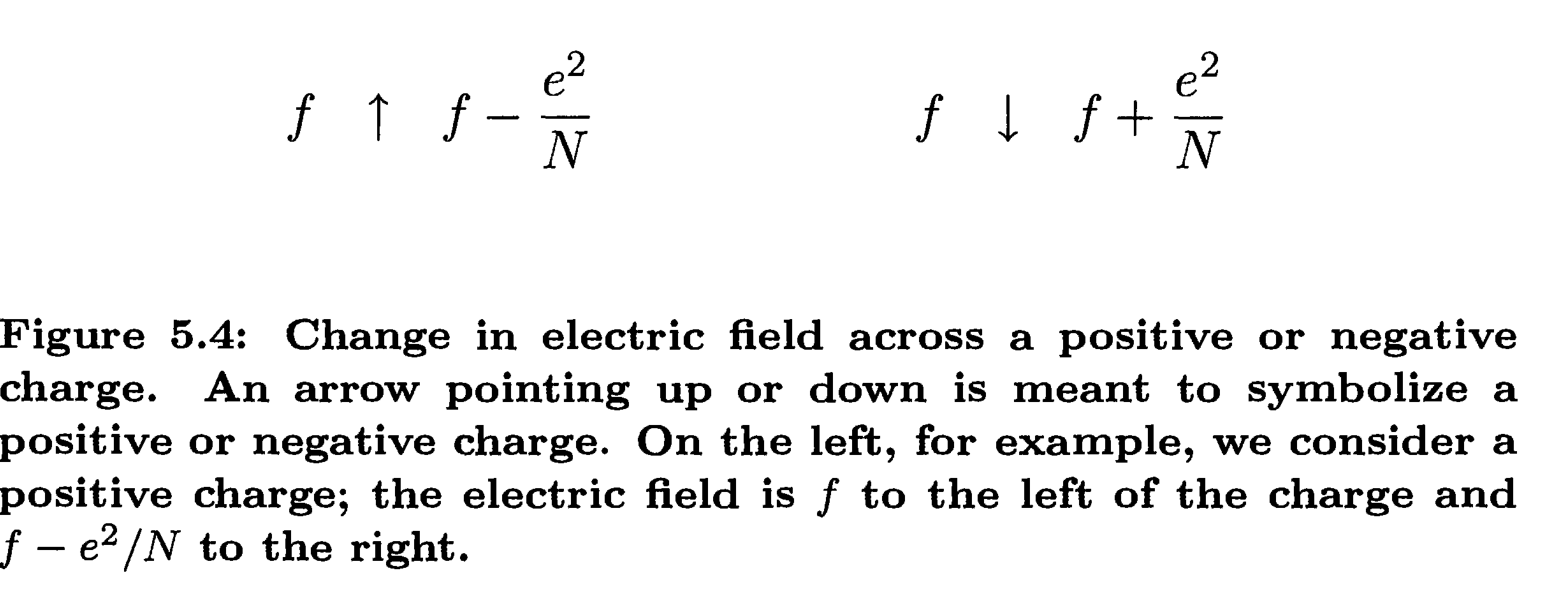
\includegraphics[width=0.76\textwidth]{figs/fig_p075_1.png}
  \caption{电场穿过一个正电荷或负电荷时的改变。向上或向下的箭头用以象征正电荷或负电荷。例如左图考虑的是正电荷：电场在电荷左侧为 $f$，在右侧为 $f-e^2/N$。（原文 Figure 5.4，p.75）}
  \label{fig:p075-1}
\end{figure}

% [Tutor Note: (5.29) 把 $\theta$ 定义为 $2\pi Nf/e^2$，其中 $f=*F_A$ 的符号依赖于二维时空的定向。用「正电荷使 $f$ 向右跳跃 $-e^2/N$」这一条（即 Gauss 定律 $\frac{N}{e^2}\partial_x f=-\rho$）可以核对系数：设 $f(-\infty)=f_0$ 而总电荷为 $Q=\int\rho\,dx$，则 $f(+\infty)=f_0-e^2Q/N$，于是 $\theta(+\infty)-\theta(-\infty)=-2\pi Q$。这既说明 $\theta$ 只有在电荷量子化（$Q\in\mathbb{Z}$）时才良定义于 $\mathbb{R}/2\pi\mathbb{Z}$，也说明若把 $f$ 换成 $-*F_A$，全篇的 $\theta$ 与 $f$ 会同时变号，而后文「$\theta=\pi$ 时禁闭解除」的结论不变——但若只改一处，就会得到「$\theta=0$ 时禁闭解除」的错误结论。]

电场 $f$ 的经典能量密度由作用量（5.23）（其中 $f=dA/dt$）算出为 $\frac{N}{2e^2}f^2$。如同在量子理论中一样，对（5.29）中固定的 $\theta$ 值，存在唯一的极小值，在某个 $f=f_0$ 处取到，只要 $\theta\neq\pi$。

% ===== 原文 p.76 =====
任何合法的位形相对于真空能量必须具有有限的能量。因此，若 $\theta\neq\pi$，当 $x\to\pm\infty$ 时必须有 $f(x)\to f_0$。利用上面关于电场穿过电荷时跳跃的公式，我们看到，一个有限能量位形的总电荷为零。这意味着存在禁闭（confinement）——不可能有单个带电粒子，也不可能有任何其他总电荷非零的孤立电荷集合。另一方面，对于 $\theta=\pi$，最小能量密度在 $f_0=\pm e^2/2N$ 处取到，因此对任何有限能量位形，当 $x\to\pm\infty$ 时 $f(x)\to\pm e^2/2N$。于是存在一个只含单个粒子的有限能量位形：其电场满足 $f(-\infty)=e^2/2N$、$f(\infty)=-e^2/2N$。（见 Figure 5.5。）此时没有禁闭。而且此时有限能量位形有四个分支，取决于 $f$ 在 $\pm\infty$ 处的值。

\begin{figure}[htbp]
  \centering
  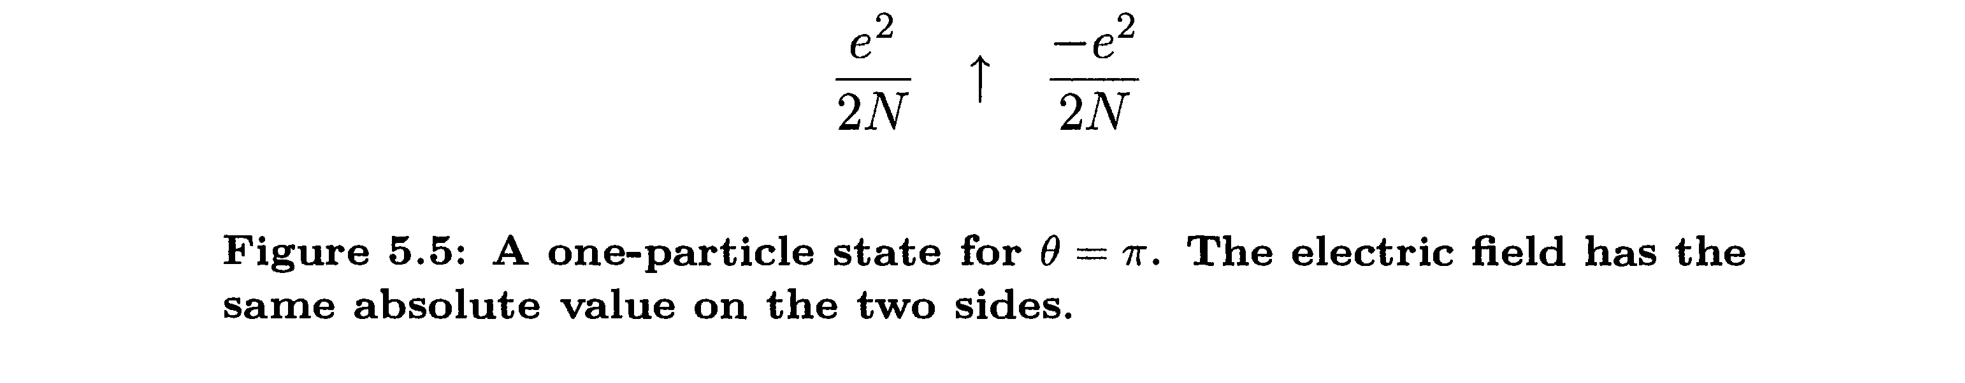
\includegraphics[width=0.76\textwidth]{figs/fig_p076_1.png}
  \caption{$\theta=\pi$ 时的一个单粒子态。电场在两侧的绝对值相同。（原文 Figure 5.5，p.76）}
  \label{fig:p076-1}
\end{figure}

请注意，在三维空间中相距 $r$ 的两个点电荷之间的 Coulomb 势正比于 $1/r$，而在一维空间中 Coulomb 势正比于 $r$。这意味着当电荷分开时势能增长，这是理解禁闭的另一种方式。

\subsection{带物质的量子理论}
% 原文 §5.7：Quantum theory with matter

现在我们要证明：只要 $\theta\neq\pi$，Lagrange 量（5.20）的量子理论中就有禁闭。这一断言就是：量子理论中每个有限能量的位形总电荷为零。

作为预备，先考虑只有物质（没有规范场）的理论。在最简单的情形 $k=N=1$，只有一个质量为 $M$ 的自由复标量场 $\phi$。这个理论的 Hilbert 空间 $\mathcal{H}_\phi$ 是 $W\oplus\overline{W}$ 的完备化对称代数（symmetric algebra），其中 $W$ 是 Poincaré 群的标量表示，质量为 $M$。存在一个使 $\phi$ 旋转的整体 $U(1)$ 对称性。相应的量子算符 $Q_\phi$，即 Noether 荷，在 $W$ 上取值为 1，在 $\overline{W}$ 上取值为 $-1$，于是在 $\mathrm{Sym}^pW\otimes\mathrm{Sym}^q\overline{W}$ 上取值为 $p-q$。这个子空间中的一个态表示 $p$ 个带正电的粒子和 $q$ 个带负电的粒子。对一般的 $k,N$，我们有 $kN$ 份这样的图像。特别地，当 $k=1$ 时存在一个整体 $SU(N)$ 对称性（在上述已经讨论过的 $U(1)$ 对称性之外）。

现在加入规范场。对于 $k=N=1$，我们有一个带单个带电标量场的 $U(1)$ 规范理论。上一段中的整体 $U(1)$ 对称性现在是局域对称性。先考虑 $\theta=0$ 的情形。对小耦合 $e^2$，我们通过量子化（5.20）的经典解构成的辛流形来构造复合系统的量子 Hilbert 空间。于是取 $\Sigma$ 为柱面 $\mathbb{R}\times S^1_V$。那么经典解的空间是 $S^1_V$ 上联络空间 $\mathcal{A}$ 的余切丛 $T^*\mathcal{A}$ 上的一个向量丛；该向量丛在平凡联络 $A=0$ 处的纤维就是 $W\oplus\overline{W}$ 底下的那个实辛向量空间。

% ===== 原文 p.77 =====
（注意，我们按复极化（complex polarization）量子化，这导致上述 Hilbert 空间 $\mathcal{H}_\phi$。）为实现规范对称性，我们必须取模去规范变换群 $\mathcal{G}$ 的辛商（symplectic quotient）。在 $S^1_V$ 上固定一个基点（无穷远点）。于是 $\mathcal{G}$ 中在基点处等于恒等的子群 $\mathcal{G}_0$ 自由地作用在 $\mathcal{A}$ 上，而商通过和乐被等同于 $U(1)$。在纯规范理论中，$T^*\mathcal{A}$ 模 $\mathcal{G}_0$ 的辛商微分同胚于 $T^*U(1)$；它的量子化 $L^2(U(1))$ 前面已经讨论过。当长度 $V\to\infty$ 时，回想唯一保持有限能量的态是真空态。经典地，真空对应于零截面，即 $T^*U(1)$ 的一个 Lagrange 子流形。常数规范变换构成的子群 $U(1)\subset\mathcal{G}$ 平凡地作用在 $\mathcal{A}$ 上——从而平凡地作用在 $T^*\mathcal{A}$ 上——因此不进入纯规范理论。在带物质的理论中，模 $\mathcal{G}_0$ 的辛商是 $T^*U(1)$ 上的一个向量丛，在恒等元处的纤维为 $W\oplus\overline{W}$。现在常数规范变换通过标量乘法非平凡地作用在纤维上。为实现这个对称性，我们有两种选择：我们可以量子化辛商，也可以考虑 Hilbert 空间中相应量子算符 $N_e$ 所湮灭的子空间。先采用后一种做法，我们看到，在无穷体积极限下，实现 $U(1)$ 之前的量子 Hilbert 空间就是 $\mathcal{H}_\phi$，因为规范场只贡献真空态。算符 $N_e$ 就等于 $Q_\phi$。因此理论的 Hilbert 空间是总电荷 $Q_\phi=0$ 的态构成的子空间。于是，正如在经典理论中一样，我们有禁闭。存在质量间隙（mass gap），最小质量为 $2M$。在小耦合理论中，定性的图像相同。

如果改为取 $W\oplus\overline{W}$ 模 $U(1)$ 的辛商，我们会被引到一个奇异空间。动量映射（moment map）是 $\mu(w,\overline{w}')=|w|^2-|\overline{w}'|^2$，而 $\mu^{-1}(0)$ 在 $(0,0)$ 处奇异。在量子化中，这个奇异点对应于真空，并且不难启发式地看出，我们会被引到与前面相同的描述。

% [Tutor Note: 这里的动量映射写作 $\mu(w,\overline{w}')=|w|^2-|\overline{w}'|^2$，第二个变量上多了一撇，疑为排印笔误：$U(1)$ 以权 $+1,-1$ 分别作用在 $W$ 与 $\overline{W}$ 上，其动量映射应写成同一个复坐标 $w$ 的 $\mu(w,\overline w)=|w|^2-|\overline w|^2$（这与正文「在 $(0,0)$ 处奇异」相容——零点集是锥面 $|w|=|\bar w|$，其顶点奇异）。若真按字面把 $w$ 与 $\bar w'$ 当作两个独立变量，$\mu^{-1}(0)$ 就是光滑流形而非奇异空间，后面的论证便不成立。另注意这里没有写出 $U(1)$ 生成元的归一化因子，它不影响零点集。]

现在允许 $\theta\neq0$。用几何量子化的语言来说，$T^*U(1)$ 上的预量子线丛（prequantum line bundle）现在被 $L_\theta\to U(1)$ 的拉回所扭化。量子态对应于给定极化的「Bohr–Sommerfeld」叶（leaves），它们是柱面 $T^*U(1)$ 中等间距的平行圆。更确切地说，若 $p$ 是余切空间中的（动量）坐标，则这些圆出现在 $p=n-\theta/2\pi$ 处，$n$ 取整数值。相应量子态的能量（在纯规范理论中）由（5.26）给出；而当 $V\to\infty$ 时我们只保留最靠近 $p=0$ 的那个（些）圆，它对应于真空态。若 $\theta\neq\pi$，这样的圆是唯一的，我们得到与上面相同的禁闭图像。对于 $\theta=\pi$，这样的圆有两个，对应于两个真空态。因此，在带物质的理论中，在模去常数规范变换之前，我们必须量子化两份不相交的 $W\oplus\overline{W}$，以得到 $\mathcal{H}_\phi\oplus\mathcal{H}_\phi$。如果像以前一样给每个真空态指定零电荷，那么对应于 $U(1)$ 对称性的算符 $N_e$ 就是 $Q_\phi\oplus Q_\phi$。被 $Q_\phi\oplus Q_\phi$ 湮灭的 $\mathcal{H}_\phi\oplus\mathcal{H}_\phi$ 的子空间，恰好是前面所见的系统的两份拷贝，每份带一个真空。这是量子理论的两个「实现」（realization），每个都有一个大小接近 $2M$ 的质量间隙。我们也可以构造包含单个电荷、能量约为 $M$ 的态，其中当 $x\to-\infty$ 时看到理论的一个实现或真空，而当 $x\to+\infty$ 时看到另一个。这些态就是在两个真空之间插值的「孤子」（soliton）；我们将在第 9 讲讨论这类态（主要是在可以用另一种拓扑论证看到它们的场合）。

% ===== 原文 p.78 =====
为论证这些启发式的图像，我们来做计算。由（5.20）可见 Hamilton 量为
\begin{equation}
  \tag{5.30}
  \label{eq:5-30}
  H=\int_{-\infty}^{\infty}dx\left(\frac{1}{2}|\pi_\phi|^2+|d_A\phi|^2+M^2|\phi|^2+\frac{N}{2e^2}|f_A|^2\right),
\end{equation}
其中 $\phi$ 是 $\mathbb{R}$ 上的场。这里 $\pi_\phi$ 是 $\phi$ 的共轭动量，$f=f_A$ 同前是曲率的 Hodge 星。我们把 $A$ 的运动方程代入，从而导出 $\phi$ 的有效 Hamilton 量。后者由（5.20）的 Lagrange 量对 $A$ 变分得到：
\begin{equation}
  \tag{5.31}
  \label{eq:5-31}
  \frac{N}{e^2}\frac{df}{dx}=j,
\end{equation}
其中流为
\[
  j=\phi\pi_\phi-\overline{\phi\pi_\phi}.
\]
我们积分（5.31）得到
\begin{equation}
  \tag{5.32}
  \label{eq:5-32}
  f(x)=\frac{e^2}{N}\left\{\int_{-\infty}^{\infty}dy\,G(x-y)j(y)+c\right\}
\end{equation}
其中 $c$ 为某个常数，而
\[
  G(x-y)=\begin{cases}1,&x\ge y;\\ 0,&x<y.\end{cases}
\]
请注意
\begin{equation}
  \tag{5.33}
  \label{eq:5-33}
  \lim_{x\to-\infty}f(x)=\frac{e^2c}{N}.
\end{equation}
代入（5.30）我们看到
\[
  H=H_0+\Delta H,
\]
其中 $H_0$ 是自由标量粒子的 Hamilton 量（若在 $A=0$ 处计算），而
\[
  \Delta H=\frac{e^2}{2N}\int_{-\infty}^{\infty}dx\left\{\int_{-\infty}^{\infty}dy\,G(x-y)j(y)+c\right\}^2.
\]
微扰项 $\Delta H$ 是非局域的，并且是奇异的。

% [Tutor Note: 由 (5.31) 到 (5.32) 用的是 $dG(x-y)/dx=\delta(x-y)$，而 $G$ 取成阶跃函数这一步同时选定了常数 $c$ 的含义：把 (5.32) 取 $x\to-\infty$ 即得 $f(-\infty)=e^2c/N$，也就是 (5.33)。注意 $G(x-y)=1$（$x\ge y$）意味着 $f(x)$ 只累积 $x$ 左侧的电荷，若把阶跃函数取成反向（$x\le y$ 时为 1），则 $c$ 会变成 $f(+\infty)N/e^2$，$c\to-c$，而 (5.34) 中 $Q_\phi+2c$ 的符号随之翻转，禁闭的判据看上去就反了。另外 $j=\phi\pi_\phi-\overline{\phi\pi_\phi}$ 与通常的 $U(1)$ 流 $i(\overline\phi\partial_t\phi-\phi\partial_t\overline\phi)$ 相差一个因子 $i$（此处 $j$ 是反厄米的）；由于 $\Delta H$ 只含 $j^2$，这个 $i$ 在能量中不起作用，但在把 (5.34) 与 $Q_\phi$ 的本征值（整数）比较时必须留意。]

现在我们必须确定使 $\Delta H$ 有限的那些态 $\Psi$ 构成的子空间。先考虑 $c=0$。这时 $\langle\Psi|\Delta H|\Psi\rangle$ 有限当且仅当
\[
  \lim_{x\to\infty}\langle\Psi|f(x)|\Psi\rangle=0,
\]
其中 $f(x)$ 由（5.32）定义。现在
\[
  \lim_{x\to\infty}\int_{-\infty}^{\infty}dy\,G(x-y)j(y)=\int_{-\infty}^{\infty}dy\,j(y)=Q_\phi
\]
是 Hilbert 空间 $\mathcal{H}_\phi$ 中的电荷算符。因此，若 $c=0$，我们就得到禁闭：
\[
  \langle\Psi|Q_\phi|\Psi\rangle=0.
\]

% ===== 原文 p.79 =====
一般地，$c$ 通过（5.33）与（5.29）同 $\theta$ 相联系：
\[
  |c|=\min_n\left(\frac{\theta}{2\pi}+n\right).
\]
这就是 $-\infty$ 处电场之值。此外，我们从 $\Delta H$ 中减去一个（无穷大的）常数，以计入无穷远处的非零能量：
\[
  (\Delta H)_{\mathrm{normalized}}=\frac{e^2}{2N}\int_{-\infty}^{\infty}dx\left[\left\{\int_{-\infty}^{\infty}dy\,G(x-y)j(y)+c\right\}^2-c^2\right].
\]
它在满足
\begin{equation}
  \tag{5.34}
  \label{eq:5-34}
  Q_\phi(Q_\phi+2c)|\Psi\rangle=0
\end{equation}
的态 $\Psi$ 上有限，即 $Q_\phi|\Psi\rangle=0$ 或 $Q_\phi|\Psi\rangle=-2c$。对于 $\theta\neq\pi$，唯一的可能是 $Q_\phi|\Psi\rangle=0$，于是我们得到禁闭。

% [Tutor Note: 上式（即 $|c|$ 的表达式）按原文图像逐字转写为 $\min_n\left(\frac{\theta}{2\pi}+n\right)$，但括号内显然漏了绝对值：$n$ 取遍全体整数时 $\frac{\theta}{2\pi}+n$ 无下界（$\to-\infty$），该 $\min$ 根本不存在。正确写法应为 $|c|=\min_{n}\left|\frac{\theta}{2\pi}+n\right|$，即取 $\frac{\theta}{2\pi}$ 到最近整数的距离；这与 (5.26) 中 $E_{\rm vac}\propto\min_n\left(n-\frac{\theta}{2\pi}\right)^2$ 的极小者一致，也才能给出后文 $c=\pm1/2$（$\theta=\pi$）与 $c=0$（$\theta=0$）的结论。此处应判为原文（或排版）笔误。]

对于 $\theta=\pi$，我们有 $c=\pm1/2$，而（5.34）对满足 $Q_\phi|\Psi\rangle=0$ 或 $Q_\phi|\Psi\rangle=\mp1$ 的态成立。正如在经典理论中一样，这给出四个扇区。我们按照电场在 $-\infty$ 与 $+\infty$ 处的值，把它们记为 $\mathcal{H}_{++},\mathcal{H}_{+-},\mathcal{H}_{-+},\mathcal{H}_{--}$。注意 $\mathcal{H}_{++}$ 中一个态的例子是相距很远的一对电荷–反电荷，各自的质量近似为 $M$。在电荷彼此分开的极限下，能量并不增加，所以人们当然愿意说这个理论不是禁闭的。如果我们取一个极限，让两个电荷中的一个位于固定位置而另一个趋于无穷远，那么在与第一个电荷距离固定处所作的一切局域测量都收敛到 Hilbert 空间 $\mathcal{H}_{+-}$（或 $\mathcal{H}_{-+}$，取决于被移到无穷远的那个电荷的符号以及它所取的方向）中的测量。类似地，把两个电荷都移到无穷远，人们可以在 $\mathcal{H}_{++}$ 中描述一列测量，它们收敛到 $\mathcal{H}_{--}$ 中的一个测量。在这个意义上，四个 Hilbert 空间都应看作是同一个故事的一部分。这是带多个真空的二维理论的一个普遍特征；它在二维以上没有类似物。

在禁闭的情形，对称群 $PSU(N)$ 起作用。在 $\theta=\pi$ 理论的扇区 $\mathcal{H}_{\pm\mp}$ 中，覆盖群 $SU(N)$ 起作用，因为单粒子态按 $SU(N)$ 的基本表示（fundamental representation）及其对偶表示变换。所以对称群是 $PSU(N)$，但 $\theta=\pi$ 时是 $SU(N)$。

$k>1$ 的故事是类似的。

\subsection{参考文献与交叉引用}

大型 $N$ 极限的讨论见 [I-Renorm Groups] 的第 4 讲、本系列的第 4 讲，以及 [I-Homework] 的习题 FE4。对称性破缺的讨论见本系列第 1 讲。

靶空间为复射影空间的 $\sigma$ 模型的大 $N$ 极限，在下列文献中被分析：

\begin{itemize}
\item A. D'Adda, M. Luscher, P. Di Vecchia, \emph{A $1/N$ expandable series of nonlinear sigma models with instantons}, Nucl. Phys. \textbf{B146} (1978), 63--76.
\item E. Witten, \emph{Instantons, the quark model, and the $1/N$ expansion}, Nucl. Phys. \textbf{B149} (1979), 285--320.
\end{itemize}

关于带质量电荷的弱耦合二维规范理论的讨论，见

\begin{itemize}
\item S. Coleman, \emph{More about the massive Schwinger model}, Annals of Physics \textbf{101} (1976), 239--267.
\end{itemize}

% [Tutor Note: 原文文献条目 "Nucl. Phys. B146 (1978), 63--76.." 末尾有两个句点，是排印重复（本文件已按惯例只保留一个）；同一条中作者名印作 "M. Luscher" 而未加变音符号，通行拼写为 Lüscher。这两处均不影响文献识别。]


\clearpage
% 原文 pp.81–90（印刷 pp.1199–1208）
\section{Lecture 6：Bose–Fermi 对应及其应用}

\begin{keytakeaways}
本讲在二维（欧氏）时空中建立含费米子的 $U(1)$ 规范理论与自由玻色子之间的\textbf{玻色化}图像：无质量费米子的手征流代数与半径 $R=1/\sqrt2$ 的角度值玻色场的顶点算子代数等同，其定量表达是算子对应 $\xi(\psi_\pm)=e^{\pm i\phi_\pm}$ 与 Jacobi 三重积恒等式所给出的配分函数恒等式。所用数学工具是 Spin 丛上 Dirac 算子的指标、Pfaffian 线丛的曲率（它给出左右表示二次指标相等这一反常抵消条件）以及 Riemann 面上的整体路径积分恒等式。主要结论有三：手征对称性因测度变换带上因子 $e^{i\gamma I}$ 而反常，从而 $\theta$ 角可被吸收进复质量 $\tilde m=me^{-i\theta}$；四费米子耦合理论在玻色变量下是自由的（$\beta$ 函数为零），而 sine-Gordon 模型在 $R=1/\sqrt2$ 时等价于自由有质量费米子（massive Thirring 模型）；把该对应用于规范理论，可在 $m_*$ 小时得到显式的有效势 $U(\phi)$，其极小在 $\theta=\pi$ 处的行为与 Ising 型临界点相联系。
\end{keytakeaways}

% ===== 原文 p.81 =====
\subsection{含费米子的二维规范理论}
% 原文 §6.1

今天我们考虑含费米子的二维规范理论。我们将使用欧氏（Euclidean）拉格朗日量。

在 2 维时，两个旋量表示 $S_+,S_-$ 都是一维且复的。它们由公式 $\theta\mapsto e^{\pm i\theta/2}$，$\theta\in[0,4\pi)$ 定义，其中 $\theta$ 是 $\mathrm{Spin}(2)$ 上的参数。

设 $\Sigma$ 是一张给定了 Spin 结构（Spin structure）的 Riemann 面。于是 $S_+,S_-$ 定义了 $\Sigma$ 上的全纯线丛，它们被称为 Spin 丛（Spin bundles），并用同一个字母记之。我们有 $S_+\otimes S_-=\mathbb{C}$，以及 $S_+^2=T\Sigma$、$S_-^2=T^*\Sigma$。$\Pi S_-$（相应地 $\Pi S_+$）的截面将被称为左行（相应地右行）费米子，这是与 Minkowski 图像类比而得名的。

我们用 $D_+:S_-\to S_+$、$D_-:S_+\to S_-$ 记 Spin 丛中相应的 Dirac 算子。

我们将做规范群为 $G$（一个紧 Lie 群）的规范理论。设 $E_L,E_R$ 是 $G$ 的正交、幺模（unimodular）表示。设 $P$ 是 $\Sigma$ 上的主 $G$-丛，并用 $E_R,E_L$ 记与表示 $E_R,E_L$ 相伴的正交向量丛。设 $\psi_+,\psi_-$ 分别是丛 $E_R\otimes S_+$、$E_L\otimes S_-$ 的截面。

含费米子的二维规范理论的拉格朗日量为

\begin{equation}
  \tag{6.1}
  \label{eq:6-1}
  \mathcal{L}=\int d^2x\left(\frac{1}{4e^2}|\ast F_A|^2+\frac{1}{4\pi}\overrightarrow{\bar\psi}_+\,\overrightarrow{D^A_-}\,\overrightarrow{\psi}_++\frac{1}{4\pi}\overrightarrow{\bar\psi}_-\,\overrightarrow{D^A_+}\,\overrightarrow{\psi}_-\right),
\end{equation}

其中 $A$ 是 $P$ 中的联络，而 $D^A_\pm$ 是相应的 Dirac 算子。

% [Tutor Note: (6.1) 中费米子动能项的系数是 $1/4\pi$，而一旦按 (6.4) 把 $\mathbb{R}$ 上的实二维表示 $E$ 分解为复分量 $(\psi_\pm,\bar\psi_\pm)$，同一项的系数就变成 $1/2\pi$。这不是笔误：实表示的两个实分量各贡献一份动能。若在此处误把 $E$ 当作复一维表示，则 (6.4) 之后的玻色化系数（$|d\phi|^2$ 的 $(1+g)/8\pi$ 与质量项的 $m/2\pi$）会整体差一个因子 2。另注意箭头的含义：$\overrightarrow{\bar\psi}$ 是 (6.4) 下方所定义的“行向量”记号，见 p.82。]

为了使这个理论在量子力学上说得通，表示 $E_L,E_R$ 还必须满足一个附加条件。为导出这个条件，回顾 (6.1) 的配分函数由下式给出

\begin{equation}
  \tag{6.2}
  \label{eq:6-2}
  Z=\int DA\int D\overrightarrow{\bar\psi}_+\,D\overrightarrow{\bar\psi}_-\,e^{-\mathcal{L}}.
\end{equation}

（在此积分中，我们对所有拓扑类型的主丛求和）。费米子积分容易计算：它等于 $I_A=\mathrm{Pf}(D^A_-|_{E_R})\mathrm{Pf}(D^A_+|_{E_L})$，其中\footnote{原文页脚注：\emph{Notes by Pavel Etingof and David Kazhdan}——本讲笔记由 Pavel Etingof 与 David Kazhdan 整理。}

% ===== 原文 p.82 =====
$\mathrm{Pf}$ 表示 Pfaffian（普法夫式）。表达式 $I_A$ 是 Pfaffian 线丛 $B=\mathrm{Pf}(D^A_-|_{E_R})\mathrm{Pf}(D^A_+|_{E_L})$ 在联络的规范等价类空间上的一个截面。为使对 $A$ 的积分有意义，这个表达式应当是一个函数，亦即丛 $B$ 必须是平凡的。可以证明（利用 Pfaffian 线丛上联络曲率的标准数学公式），这归结为如下条件

\begin{equation}
  \tag{6.3}
  \label{eq:6-3}
  \operatorname{Tr}\big(\rho_L(t)\rho_L(t')\big)=\operatorname{Tr}\big(\rho_R(t)\rho_R(t')\big),
\end{equation}

其中 $t,t'\in\mathfrak{g}$，$\mathfrak{g}$ 是规范群 $G$ 的 Lie 代数，而 $\rho_{L,R}:\mathfrak{g}\to SO(E_{L,R})$ 是表示映射。若 $G$ 单，且 $E_L,E_R$ 不可约，则此条件意味着 $E_L,E_R$ 的 Casimir 相同。方程 (6.3) 称为反常抵消（anomaly cancellation）条件。从另一个观点看，它（在四维情形下）已在 Lecture 3.7 中描述过。

% [Tutor Note: 作者说“可以证明”而省略的，是 Pfaffian 线丛上 Quillen 型联络的曲率公式：其曲率正比于 $\operatorname{Tr}\rho^2(F)$ 的积分，因此 $B$ 的平凡性要求左右两个表示的二次指标相等，即 (6.3)。注意 (6.3) 只对 $\mathfrak{g}$ 中元素成立、并未要求 $E_L\cong E_R$ 作为表示同构；对 $G=U(1)$ 它退化为“左右荷的平方相等”，故 $E_L=E_R$ 只是一维情形下的结论。]

今天我们将考虑一个简单情形：$G=U(1)$，且 $E_L,E_R$ 是不可约的二维实表示。此时 (6.3) 说明 $E_L,E_R$ 相同：$E_L=E_R=E$。我们将取 $E=\mathbb{C}$，度量为 $|z|^2$，$U(1)$ 通过乘法作用（但要记住张量积 $S_\pm\otimes E$ 是在 $\mathbb{R}$ 上取的）。我们把 $S_\pm\otimes E$ 分解为两个二维表示的直和。利用这个分解，我们将写 $\overrightarrow{\bar\psi}_\pm=(\psi_\pm,\bar\psi_\pm)$，其中对 $z\in U(1)$ 有 $z(\psi,\bar\psi)=(z\psi,\bar z\bar\psi)$。

在新记号下，拉格朗日量 (6.1) 具有形式

\begin{equation}
  \tag{6.4}
  \label{eq:6-4}
  \mathcal{L}=\int d^2x\left(\frac{1}{4e^2}|\ast F_A|^2+\frac{1}{2\pi}\bar\psi_+D^A_-\psi_++\frac{1}{2\pi}\bar\psi_-D^A_+\psi_-\right),
\end{equation}

我们还可以给这个拉格朗日量加上一个拓扑项：

\begin{equation}
  \tag{6.5}
  \label{eq:6-5}
  \mathcal{L}_\theta=\mathcal{L}-\frac{i\theta}{2\pi}\int F,
\end{equation}

以及一个质量项：

\begin{equation}
  \tag{6.6}
  \label{eq:6-6}
  \mathcal{L}_{\theta,m}=\mathcal{L}_\theta+\frac{m}{2\pi}\bar\psi_-\psi_++\frac{\bar m}{2\pi}\bar\psi_+\psi_-,
\end{equation}

（这里 $m$ 是复的）。

\subsection{手征对称性}
% 原文 §6.2

手征对称性（chiral symmetry）是经典拉格朗日量 (6.4) 或 (6.5) 的一个 $U(1)$-对称性，由下式给出

\begin{equation}
  \tag{6.7}
  \label{eq:6-7}
  \psi_+\to\psi_+,\qquad \psi_-\to e^{i\gamma}\psi_-.
\end{equation}

这个对称性被质量项破坏。然而，即便没有质量项，由于下述拓扑理由，这个对称性也可能在量子力学上被破坏。

设时空是一张闭 Riemann 面。于是在手征对称性下，“测度” $\mu=D\psi_-D\bar\psi_-$ 变换为 $\mu\to e^{i\gamma I}\mu$，其中 $I$ 是算子 $D^A_+:S_-\otimes_{\mathbb{C}}E\to S_+\otimes_{\mathbb{C}}E$ 的指标（index）。“证明”：设 $\{\psi_-\}$ 记

% ===== 原文 p.83 =====
$S_-$ 的荷（charge）为 $1$ 的截面空间，而 $\{\bar\psi_-\}$ 记荷为 $-1$ 的对应空间。则形式上 $I=\dim(\{\psi_-\})-\dim(\{\bar\psi_-\})$；由于 $(\{\bar\psi_-\})=(\{\psi_-\})^*$，我们有 $I=\dim(\{\psi_-\})-\dim(\{\psi_+\})=\mathrm{ind}\big(D^A_+|_{S_+\otimes_{\mathbb{C}}E}\big)$。这里 $\mathrm{ind}$ 表示所述算子的指标。

% [Tutor Note: 这一步“由 $(\{\bar\psi_-\})=(\{\psi_-\})^*$ 得 $\dim(\{\bar\psi_-\})=\dim(\{\psi_+\})$”隐含使用了 $S_-\otimes S_+=\mathbb{C}$（见 p.81），即复共轭把荷 $-1$ 的 $S_-$ 截面空间同构地送到荷 $+1$ 的 $S_+$ 截面空间。若忽略这点而误以为 $\bar\psi_-$ 与 $\psi_-$ 的截面空间同维，指标将恒为零，反常就消失了。此外 $I=c_1(P)$ 是 Atiyah–Singer 指标定理在二维的显式形式（$S_\pm$ 复一维、$E$ 复一维时，$\mathrm{ind}$ 就是耦合后的度数公式）；$1/2\pi$ 这一归一化必须与 (6.5) 中 $\theta$ 项的 $1/2\pi$、以及下文 $dJ_A=F/2\pi$ 的结论取自同一套约定，任何一处改号都要三处同时改。]

已知指标 $I$ 等于 $c_1(P)=\int\frac{F_A}{2\pi}$。因此，由于丛 $P$ 在拓扑上可以非平凡，手征对称性在量子理论中被破坏。

这个效应称为反常（anomaly）：一个经典对称性在量子力学上不成立，因为测度不是不变的。与 Lecture 1 中讨论的自发对称性破缺（spontaneous symmetry breaking）的差别在于：在自发对称性破缺的情形，经典对称性在量子理论中确实存在，只是未被实现。对称性上的反常意味着该对称性根本不是量子理论的对称性。再说一遍——因为这是一点虽然初等却非常重要的地方：有反常的对称性是经典对称性，而不是量子理论的对称性；而自发破缺的对称性是量子理论的对称性，但并不保持真空不变。（与自发对称性破缺不同，反常甚至可以出现在一个时空维数下。）

下面用流（current）的语言讨论手征对称性破缺的机制。经典地，手征对称性由流

\begin{equation}
  \tag{6.8}
  \label{eq:6-8}
  J_A=\bar\psi_-\psi_-
\end{equation}

生成（这是 $(0,1)$ 型的一次形式），它当然是守恒的：$dJ_A=0$。在量子力学上，这个微分方程可以被形变：$dJ_A=\mathcal{O}$，其中 $\mathcal{O}$ 是某个取值于曲面上二次形式的算子。通过列举所有可能的算子，不难证明能出现的算子（up to a factor）只有一个：它就是曲率算子 $F$。于是 $dJ_A=\alpha F$，其中 $\alpha$ 是常数，而先前的拓扑计算表明 $\alpha=1/2\pi$。也可以通过研究 Feynman 图来建立关系 $dJ_A=F/2\pi$；这最初就是这样做的。

当存在有反常的对称性时，关联函数以非常简单的方式依赖于 $\theta$。我们将在拉格朗日量 (6.5) 的背景下说明这一陈述。设 $\mathcal{O}_i$ 是任意算子，使得在手征对称性下 $\prod_i\mathcal{O}_i\to e^{in\gamma}\prod_i\mathcal{O}_i$。则上述指标计算蕴含着：关联子 $\langle\prod\mathcal{O}_i\rangle$ 的所有非平凡贡献都来自 $c_1=n$ 的丛 $P$。（这正是“测度乘以 $\prod_i\mathcal{O}_i$ 在该对称性下不变”这一条件。）于是这个关联子具有形式 $e^{in\theta}\langle\prod\mathcal{O}_i\rangle_0$，其中 $\langle\prod\mathcal{O}_i\rangle_0$ 与 $\theta$ 无关。例如 $\langle\psi_-\psi_+^*\rangle=Ce^{i\theta}$，其中 $C$ 与 theta 无关。

若我们考虑的不是 (6.5)、而是带质量项的拉格朗日量 (6.6)，则上述论证表明

\begin{equation}
  \tag{6.9}
  \label{eq:6-9}
  \Big\langle\prod\mathcal{O}_i\Big\rangle(m,\theta)=e^{in\theta}\Big\langle\prod\mathcal{O}_i\Big\rangle_0(\tilde m),
\end{equation}

其中 $\tilde m=me^{-i\theta}$。因此，理论真正重要的参数是 $\tilde m$，我们将把它写成 $m_*e^{-i\theta_*}$，$m_*\ge0$。本讲的目标就是把这个理论作为 $\tilde m$ 的函数来研究。

% ===== 原文 p.84 =====
\subsection{带质量费米子的二维规范理论的行为}
% 原文 §6.3

现在我们要描述由拉格朗日量 (6.6) 定义的这一理论的行为，随后再为我们的论断提供依据。

首先，我们将看到：对大的 $m_*$（即 $m_*\gg e$），该理论类似于上一讲中考虑过的带质量玻色子的二维规范理论。特别地，它有质量隙（mass gap）。它在 $\theta\ne\pi$ 时具有唯一真空，而在 $\theta=\pi$ 时有两个真空。宇称（parity）或空间取向反转（$t\to t$，$x\to-x$）这一离散对称性，其作用为 $m_*\to m_*$、$\theta_*\to-\theta_*$，在 $\theta_*=0$ 或 $\pi$ 时是理论的对称性。对大的 $m_*$，若 $\theta_*=0$ 则宇称不变，若 $\theta^*=\pi$ 则宇称破缺。

接下来我们将证明：对 $\tilde m=0$，理论实际上是自由的，事实上它在一次变量代换之后成为一个自由的有质量理论。因此对小 $m_*$（即 $m_*\ll e$），理论有唯一真空与质量隙。对小 $m_*$，无论 $\theta$ 是 $0$ 还是 $\pi$，宇称都不破缺。

在 $\theta=\pi$ 以及 $m_*$ 的某个 $e$ 阶临界值处，人们相信理论会失去质量隙；事实上人们相信，在临界值 $\tilde m=-m_c$ 处理论实际上是共形的（conformal），并且同构于一个自由实费米子的理论。但这些断言的论证并不那么精确。

% [Tutor Note: 本段末尾把 $\theta_*$ 误排为 $\theta^*=\pi$（上标），与全篇的下标记号不一致，应以 $\theta_*=\pi$ 为准；$\theta_*$ 是 $\tilde m=m_*e^{-i\theta_*}$ 中的相位，其取值在 $[0,2\pi)$，与 (6.7) 中手征参数 $\gamma$ 无关，切勿混同。]

\subsection{重费米子}
% 原文 §6.4

本节我们研究 $m_*\gg e$ 的情形。此时我们可以把我们的理论视为 $e=0$ 之理论的微扰，微扰参数为 $\lambda=e/m_*$。在 $\lambda=0$ 处，我们有一个二维纯规范理论（它是自由的）与有质量费米子的自由理论的直积（为稳妥起见，我们应引入 $B=A/e$；这是合理的，因为当 $e=0$ 时只有平凡 $U(1)$-丛对路径积分有贡献）。

情形与我们上周研究过的玻色情形类似，可以用类似的论证来分析。也就是说，$e=0$ 的自由理论的小 $e$ 微扰是奇异的（singular）。形变后理论的状态空间实际上比未形变理论的状态空间更小。更确切地说，费米子禁闭（confinement）发生了：唯一允许的态（对 $\theta\ne\pi$）是总荷为 $0$ 的态（这里 $\psi_\pm$ 的荷为 $1$，$\bar\psi_\pm$ 的荷为 $-1$，且 $\theta\in[0,2\pi)$）。特别地，费米子只能成对、成四地出现，单个费米子不可能存在。

与玻色情形一样，由形变论证可知理论有质量隙（形变是奇异的这一事实并不使该论证失效，因为 Hilbert 空间不会增加，只会变小）。更确切地说，$\theta\ne\pi$ 时有一种实现，$\theta=\pi$ 时有两种（与纯规范理论一样），而任何实现都有质量隙。

\subsection{Bose–Fermi 对应}
% 原文 §6.5

在研究轻费米子的情形之前，我们先考虑 Bose–Fermi 对应（Bose–Fermi correspondence），它在研究小 $m_*$ 的情形时会有用。

考虑两个二维自由场论

% ===== 原文 p.85 =====
\begin{enumerate}
\item 由拉格朗日量
\begin{equation}
  \tag{6.10}
  \label{eq:6-10}
  \mathcal{L}_f=\frac{1}{2\pi}\int d^2x\left(\bar\psi_-\partial_+\psi_-+\bar\psi_+\partial_-\psi_+\right)
\end{equation}
定义的费米子理论。

\item 由拉格朗日量
\begin{equation}
  \tag{6.11}
  \label{eq:6-11}
  \mathcal{L}_b=\frac{R^2}{4\pi}\int d^2x\,|d\phi|^2
\end{equation}
定义的玻色子理论。
\end{enumerate}

这两个理论是共形的（经典上与量子力学上都是），且 Virasoro 中心荷为 $1$。因此我们可以猜测它们之间可能存在某种联系。而这样的联系确实存在；它被称为 Bose–Fermi 对应。

\textbf{Remark.} 中心荷很小的共形场论非常稀少。例如对 $c<1$，它们已被 Friedan、Qiu、Shenker 完全分类（Phys. Rev. Lett, vol 52, 1984, p. 1575）。答案是：不存在连续参数，理论几乎完全由 $c$ 决定，而 $c$ 只能取一个离散的值序列。对 $c=1$，这样的分类尚不可得，但已知的例子极少，且它们全都可以用自由 Bose 场来构造。

现在让我们看看玻色理论 (6.11)。如我们在 Lecture 1 中所记得的，为使这个理论有意义，$\phi$ 必须是角度值的（angle-valued），即取值于圆周 $\mathbb{R}/2\pi\mathbb{Z}$。拉格朗日量中的常数 $R$ 具有这个圆周半径的意义。

\textbf{Remark.} 我们总是把目标圆周模型化为 $\mathbb{R}/2\pi\mathbb{Z}$，但考虑其上的各种 Riemann 度量，它们由半径 $R$ 的取值来参数化。

回顾 Lecture 1：这个理论（在其唯一的实现中）的 Hilbert 空间形如 $\mathcal{H}_b=\oplus_{k\in\mathbb{Z}}(F_b\otimes F_b^*)_k$，其中 $F_b$ 是玻色 Fock 空间。理论的算子代数 $A_b$ 由 $\phi$ 的导数（但不是 $\phi$ 本身）以及 $:e^{in\phi}:$ 生成（为简便起见，我们暂时省略冒号）。算子乘积展开（operator product expansion）由 [I-Perturbative QFT] 的 Lecture 3 中的公式 (3.9) 给出，其中 $D(x-y)=-R^{-2}\ln|x-y|$。$A_b$ 在 $\mathcal{H}_b$ 中的作用为：$\phi$ 的导数不改变 $k$，而 $:e^{in\phi}:$ 把 $(F_b\otimes F_b^*)_k$ 映到 $(F_b\otimes F_b^*)_{k+n}$。

现在考虑理论 (6.10)。这个理论的 Hilbert 空间是 $\mathcal{H}_f=F_f\otimes F_f^*$，其中 $F_f$ 由真空经全纯算子 $\psi_+,\bar\psi_+$ 生成，而 $F_f^*$ 由真空经 $\psi_-,\bar\psi_-$ 生成。算子代数 $A_f$ 由 $\psi_+,\bar\psi_+,\psi_-,\bar\psi_-$ 生成，带有自由理论的标准 OPE。

更仔细地考虑算子 $:e^{in\phi}:$，$n\in\mathbb{Z}$。如我们所知（[I-Perturbative QFT] 的 Lecture 3 与 Lecture 1；该结果可由对我们刚写下的 $D(x-y)$ 公式取指数得到），这个算子具有全纯维数与反全纯维数 $n^2/4R^2$（左右维数之和为 $n^2R^2/2$，正如我们在 [I-Perturbative QFT] 的 Lecture 3 中所见）。

% [Tutor Note: 此处“左右维数之和为 $n^2R^2/2$”与前面的 $h=\bar h=n^2/4R^2$ 不能同时成立：$h+\bar h=n^2/2R^2$。由 p.86 紧接着的条件“$n^2/2R^2$ 必须是整数”（$e^{in\phi_+}$ 的单值性）可以判定，正确的和应为 $n^2/2R^2$，原文的 $n^2R^2/2$ 疑为 $R\to1/R$（T-对偶）写法残留的笔误。注意顶点算子的维数在 $R\to1/R$ 下并非不变，交换的是 $e^{in\phi}$ 与磁型/电型算子。]

经典地，算子 $e^{in\phi}$ 局部地分解为全纯因子与反全纯因子之积：$e^{in\phi}=e^{in\phi_+}e^{in\phi_-}$，其中 $\phi=\phi_++\phi_-$，且 $\partial_-\phi_+=\partial_+\phi_-=0$。（当然，这里 $\phi_+,\phi_-$ 只定义到相差一个常数。）并不显然的是，人们可以定义算子 $e^{in\phi_\pm}$，而这样的算子

% ===== 原文 p.86 =====
并不出现在代数 $A_b$ 中。但不妨设想一下 $e^{in\phi_\pm}$ 有意义。那么我们就会从 $e^{i\phi}$ 的 OPE 发现，$e^{i\phi_+}$ 具有全纯维数 $1/4R^2$ 与反全纯维数 $0$，并且

\begin{align}
  & \left\langle e^{i\phi_+(x_1)}\cdots e^{i\phi_+(x_n)}e^{-i\phi_+(y_1)}\cdots e^{-i\phi_+(y_n)}\right\rangle \tag{6.12}\label{eq:6-12}\\
  & \qquad =\frac{\prod_{1\le i<j\le n}(x_i-x_j)^{1/2R^2}\;\prod_{1\le i<j\le n}(y_i-y_j)^{1/2R^2}}{\prod_{1\le i,j\le n}(x_i-y_j)^{1/2R^2}}.\notag
\end{align}

其中 $x_i,y_j$ 被视为复数。由这个公式清楚可见，为使 $e^{i\phi_+}$ 有任何意义，我们需要 $1/2R^2\in\mathbb{Z}$，使得 (6.12) 的右端是单值的函数。类似地，为使 $e^{in\phi_+}$ 有意义，$n^2/2R^2$ 必须是一个整数。

我们考虑 $e^{in\phi_+}$ 能有意义的第一个情形，即 $R=1/\sqrt2$ 且 $n=1$。此时我们有

\begin{align}
  & \left\langle e^{i\phi_+(x_1)}\cdots e^{i\phi_+(x_n)}e^{-i\phi_+(y_1)}\cdots e^{-i\phi_+(y_n)}\right\rangle \tag{6.13}\label{eq:6-13}\\
  & \qquad =\frac{\prod_{1\le i<j\le n}(x_i-x_j)\;\prod_{1\le i<j\le n}(y_i-y_j)}{\prod_{1\le i,j\le n}(x_i-y_j)}.\notag
\end{align}

由 (6.13) 清楚可见，$e^{i\phi_+}$ 的行为像费米子；更一般地，$e^{in\phi_+}$ 在 $n$ 为奇数时行为像费米子，在 $n$ 为偶数时行为像玻色子。这使我们期望：在 $R=1/\sqrt2$ 时，我们的理论与费米子的理论有关。

让我们看看为什么确实如此。我们来计算费米子关联函数 $\langle\psi_+(x_1)\cdots\psi_+(x_n)\bar\psi_+(y_1)\cdots\bar\psi_+(y_n)\rangle$。用 Wick 公式，容易求得

\begin{equation}
  \tag{6.14}
  \label{eq:6-14}
  \left\langle\psi_+(x_1)\cdots\psi_+(x_n)\bar\psi_+(y_1)\cdots\bar\psi_+(y_n)\right\rangle=\det\left(\frac{1}{x_i-y_j}\right).
\end{equation}

(6.13)、(6.14) 右端的吻合是一个著名的组合恒等式，它来自零点与极点的比较，以及无穷远处渐近行为的比较。

\textbf{Remark.} 事实上，(6.13)、(6.14) 的显式形式与“证明它们相等”无关。有关的只是零点与极点的结构，以及无穷远处的渐近行为，而这两者在两种情形下都可由 OPE 明显看出。

设 $\widehat{A}_b$ 是由 $A_b$ 与 $e^{in\phi_\pm}$ 生成的算子代数。等式 (6.13)、(6.14) 表明存在一个同态 $\xi:A_f\to\widehat{A}_b$，由 $\xi(\psi_\pm)=e^{\pm i\phi_\pm}$、$\xi(\bar\psi_\pm)=e^{\mp i\phi_\pm}$ 定义，它保持期望值。

利用 OPE，容易求得

\begin{equation}
  \tag{6.15}
  \label{eq:6-15}
  \xi(:\bar\psi_+\psi_+ :)=\lim_{\varepsilon\to0}\xi\left(\bar\psi_+(x+\varepsilon)\psi_+(x)-\frac{1}{\varepsilon}\right)=\lim_{\varepsilon\to0}\left(e^{-i\phi_+(x+\varepsilon)}e^{i\phi_+(x)}-\frac{1}{\varepsilon}\right)=-i\partial_+\phi.
\end{equation}

% [Tutor Note: (6.15) 中被减去的 $1/\varepsilon$ 是正规序的减除项：由 $\langle\phi_+(x+\varepsilon)\phi_+(x)\rangle=-\frac{1}{2R^2}\ln\varepsilon$ 可得 $e^{-i\phi_+(x+\varepsilon)}e^{i\phi_+(x)}\sim\varepsilon^{-1/2R^2}\big(1-i\varepsilon\partial_+\phi+\cdots\big)$，在 $R=1/\sqrt2$ 时奇异因子恰为 $\varepsilon^{-1}$，减去它之后极限给出 $-i\partial_+\phi$；若 $R\ne1/\sqrt2$，减除项须改为 $\varepsilon^{-1/2R^2}$，本式不能照搬。符号上：$\xi(\psi_+)=e^{+i\phi_+}$、$\xi(\bar\psi_+)=e^{-i\phi_+}$ 这一配对方式必须与 (6.15) 中 $-i\partial_+\phi$ 的负号一致，若把 $\xi(\psi_+)$ 取成 $e^{-i\phi_+}$，则 $:\bar\psi_-\psi_-:$ 的对应符号会整体反号。]

同样地，$\xi(:\bar\psi_-\psi_- :)=i\partial_-\phi$。又 $\xi(\psi_+\bar\psi_-)=e^{i\phi}$，$\xi(\psi_-\bar\psi_+)=e^{-i\phi}$。事实上，不难看出这个同态是一个同构。

% ===== 原文 p.87 =====
在 Hilbert 空间的层面上，$\xi$ 诱导出一个双分次同构 $F_f\to F_b\otimes l_2(\mathbb{Z})$（双次数 $=$（量子标度维数，荷）），其中 $e^{i\phi_+}$ 的荷与 $\psi_+$ 的荷都等于 $1$。写出相应的特征标（character）公式，我们便得到

\begin{equation}
  \tag{6.16}
  \label{eq:6-16}
  \frac{\sum_{n\in\mathbb{Z}}q^{n^2/2}z^n}{\prod_{n\ge1}(1-q^n)}=\prod_{n\ge1}\left(1+q^{n-1/2}z\right)\left(1+q^{n-1/2}z^{-1}\right),
\end{equation}

这也就是著名的 Jacobi 三重积恒等式（Jacobi triple product identity）。（这里左端是左行玻色子的配分函数，右端是费米子的类似配分函数，所用的是圆周上的 bounding spin 结构。要 a priori 地说明这才是与玻色子比较时应采用的正确 spin 结构，需要比我们所做的更为细致的分析。）

这个对应 $\xi$ 称为 Bose–Fermi 对应。

% [Tutor Note: (6.16) 是 Jacobi 三重积恒等式的“配分函数”形式，容易与通常的 $\prod(1-q^n)(1+q^{n-1/2}z)(1+q^{n-1/2}z^{-1})=\sum_n q^{n^2/2}z^n$ 混淆：注意此处左端的分子/分母关系恰好是通常恒等式除以 $\prod(1-q^n)$，即把玻色零点能（$q^{-1/24}$ 型的 Vacuum 能量）略去不写。若计及中心荷 $c=1$ 的 Casimir 能量，两侧都还应乘 $q^{-1/24}$，但阶数比较不受影响。$z$ 的幂次度量 $U(1)$ 荷，$q$ 的幂次度量标度维数，两者共同构成双分次。]

\textbf{Remark 1.} 如果圆周的半径不是 $1/\sqrt2$ 而是 $1$，那么算子 $e^{i\phi_+}$ 没有意义，因为它的两点函数会是 $(x-y)^{-1/2}$，不是单值的。然而算子 $e^{2i\phi}$ 是有定义的，它的两点函数是 $\dfrac{1}{(x-y)^2}$。这表明 $e^{2i\phi}$ 的行为像某种对称性的流。而确实，相应的模型等价于 Kac–Moody 中心荷为 $1$ 的 $SU(2)$-WZW 模型，因此它具有 $SU(2)$ 对称性。事实上，算子 $e^{\pm2i\phi_+}$ 与 $\partial_+\phi$ 的 Fourier 分量生成左行 $\widehat{SU(2)}$，而算子 $e^{\pm2i\phi_-}$ 与 $\partial_-\phi$ 的 Fourier 分量生成右行 $\widehat{SU(2)}$。

\textbf{Remark 2.} 事实上，Bose–Fermi 对应不仅在局部（在算子乘积展开的层面上）成立，而且在整体上（在任意 Riemann 面上的路径积分层面上）也成立。Bose–Fermi 对应的一个优雅的整体版本如下。对任何闭 Riemann 面 $\Sigma$，配分函数之间有如下恒等式

\begin{equation}
  \tag{6.17}
  \label{eq:6-17}
  \int D\phi\,e^{-\frac{1}{8\pi}\int|d\phi|^2}=\sum_{\varepsilon}\int D\psi_+D\bar\psi_+D\psi_-D\bar\psi_-\,e^{-\mathcal{L}_f(\psi)},
\end{equation}

其中 $\phi$ 被理解为 $\Sigma$ 到圆周的映射，$\mathcal{L}_f$ 是由 (6.10) 给出的拉格朗日量，而 $\varepsilon$ 遍历 $\Sigma$ 上的 spin 结构（$\psi_+$ 与 $\psi_-$ 取相同的 spin 结构）。若按上面解释的方式建立算子之间的对应，则对算子的关联函数也有类似的恒等式。

\subsection{非线性理论的 Bose–Fermi 对应}
% 原文 §6.6

我们已经建立了两个自由理论——一个玻色子的理论与一个费米子的理论——之间的对应。既然我们知道如何把一侧的算子与另一侧的算子等同起来，我们就可以把“在拉格朗日量中加入给定算子以微扰玻色理论”所得的非自由理论，与“加入相应算子以微扰费米理论”所得的非自由理论相比较。这引出许多惊人的结果。我们考虑几个例子。

1. 回顾在我们的对应下 $\mathcal{L}_f\to\mathcal{L}_b(1/\sqrt2)$，其中 $\mathcal{L}_b(R)$ 由 (6.11) 给出。由于 $\xi(\bar\psi_\pm\psi_\pm)=\mp i\partial_\pm\phi$，我们得到

\begin{equation}
  \tag{6.18}
  \label{eq:6-18}
  \mathcal{L}_f+\frac{1}{2\pi}\int d^2x\left(g\bar\psi_+\psi_+\bar\psi_-\psi_-\right)\to\mathcal{L}_b\left(1/\sqrt2(1+g)^{-1/2}\right).
\end{equation}

% ===== 原文 p.88 =====
这表明，出乎我们意料，拉格朗日量为 $\mathcal{L}_f+\frac{1}{2\pi}\int d^2x(g\bar\psi_+\psi_+\bar\psi_-\psi_-)$ 的理论是自由的。特别地，它的 $\beta$ 函数为零。当理论用 Bose 变量描述时这是显然的，在 Fermi 变量下却不显然。

2. 另一方面，考虑自由有质量费米子的理论，其拉格朗日量为 $\mathcal{L}_f+\frac{1}{2\pi}\int d^2x(m\bar\psi_-\psi_++\bar m\bar\psi_+\psi_-)$。利用 $\xi(\bar\psi_\pm\psi_\mp)=-e^{\mp i\phi}$，我们得到：在 $\xi$ 之下，这个自由拉格朗日量变为

\begin{equation}
  \tag{6.19}
  \label{eq:6-19}
  \mathcal{L}_b\left(1/\sqrt2\right)-\frac{1}{2\pi}\int d^2x\left(me^{i\phi}+\bar m e^{-i\phi}\right).
\end{equation}

于是我们得到另一个惊人的事实：由 (6.19) 定义的非线性理论实际上是自由的。

\textbf{Remark.} 可能看起来 (6.19) 的第二项有错误的标度维数。并非如此，因为算子 $e^{\pm i\phi}$ 的反常维数为 $1$。更确切地说，(6.19) 并不固定一个理论，而是固定依赖于动量标度 $\mu$ 的一族理论，$\mu$ 是在算子 $e^{i\phi}$ 被重整化时引入的。这个标度出现在拉格朗日量中相应项的前面，并抵消了量纲上的不符。

利用对称性 $\phi\to\phi+\theta$，我们可以把 (6.19) 化归为 $m$ 为实的情形。此时 (6.19) 看起来是

\begin{equation}
  \tag{6.20}
  \label{eq:6-20}
  \mathcal{L}_b\left(\sqrt2\right)-\frac{m}{\pi}\int d^2x\cos\phi.
\end{equation}

% [Tutor Note: 由 (6.19) 到 (6.20) 时 $R$ 从 $1/\sqrt2$ 变成 $\sqrt2$，相当于把拉格朗日量整体乘以 $4$（因 $\mathcal{L}_b(R)\propto R^2$），此时质量项系数本应同时变为 $4m/\pi$，而原文仍写 $m/\pi$。这不影响物理（整体归一化可任意，等价于重新定义 $m$），但下面 (6.21) 用 $m'$ 与 (6.20) 作比较时，必须锁定同一个归一化约定，否则会差出因子 $4$；下文 $m'$ 的系数问题正出在同一处 $R$ 的重标度上（见下条批注）。]

于是，经典运动方程为 $\Delta\phi=-4m\sin\phi$。这个方程称为 sine-Gordon 方程，它是著名的完全可积的孤子方程。量子理论也是可积的（在 Lecture 4 中我们所了解的意义上）。当然，在量子理论等价于一个自由有质量费米子理论的那个耦合值处，它不仅是可积的，而且是自由的。

现在考虑拉格朗日量

\begin{equation}
  \tag{6.21}
  \label{eq:6-21}
  \mathcal{L}_b(R)-\frac{m}{\pi}\int d^2x\cos\phi.
\end{equation}

这个拉格朗日量与 (6.20) 成比例，其中 $m'=m/2R^2$，所以经典上两个拉格朗日量等价。然而在量子力学上并非如此，因为把拉格朗日量乘以一个常数确实会影响量子理论。事实上，理论现在本质上依赖于 $R$。若 $R=1/\sqrt2$，理论是自由的。对一般的 $R$ 它不是自由的。映射 $\xi$ 表明，对一般的 $R$，理论等价于拉格朗日量为

\begin{equation}
  \tag{6.22}
  \label{eq:6-22}
  \mathcal{L}_f+\int d^2x\left(m\bar\psi_-\psi_++m\bar\psi_+\psi_-+g\bar\psi_+\psi_+\bar\psi_-\psi_-\right),
\end{equation}

的费米理论，其中 $R=1/\sqrt2(1+g)^{-1/2}$。

% [Tutor Note: “$m'=m/2R^2$”疑为 $m'=2m/R^2$ 之误，可直接验证：$\mathcal{L}_b(R)=(R^2/2)\mathcal{L}_b(\sqrt2)$，故若 (6.21)$\,=(R^2/2)\times$(6.20)$|_{m'}$，则 $(R^2/2)(m'/\pi)=m/\pi$，即 $m'=2m/R^2$。取 $R=1/\sqrt2$（即 $g=0$）检验：此时 $m'=4m$，$(1/4)\big[\mathcal{L}_b(\sqrt2)-\frac{4m}{\pi}\int\cos\phi\big]=\mathcal{L}_b(1/\sqrt2)-\frac{m}{\pi}\int\cos\phi$，恰为 (6.21) 在 $R=1/\sqrt2$ 处的值，亦即自由费米子理论；而按原文的 $m'=m/2R^2=m$ 只会得到 $\frac{m}{4\pi}\int\cos\phi$，与“$R=1/\sqrt2$ 时理论自由”矛盾。]

% [Tutor Note: 关于 $g$ 的依赖，原文内部也不自洽：由 (6.18)、(6.22) 得 $R=(1/\sqrt2)(1+g)^{-1/2}$，即 $R^2=(1+g)^{-1}/2$，代入 (6.11) 应得 $|d\phi|^2$ 的系数 $R^2/4\pi=1/(8\pi(1+g))$；然而 (6.24) 与 (6.27) 中该系数一律写作 $(1+g)/8\pi$。二者只在 $g=0$ 时一致，故其中必有一处笔误（若以 (6.24)/(6.27) 为准，则 (6.18)、(6.22) 中的指数应为 $+1/2$）。此点直接影响“大 $g$ 对应大半径（弱耦合）”还是“大 $g$ 对应小半径”的物理判断，阅读时务必以自己重算的系数为准。]

如我们提到的，由拉格朗日量 (6.21) 描述的理论在 $R\ne1/\sqrt2$ 时不是自由的，但是可积的。它的 $S$ 矩阵可以用我们在 Lecture 4 中讨论过的方法计算。这个理论对大 $R$（即在经典

% ===== 原文 p.89 =====
极限下）的可解性，与 sine-Gordon 方程在经典层面的完全可积性有关。

现在我们想把 Bose–Fermi 对应应用于规范理论。若 $m$ 很小或为零，这将给出严格而精确的结果。考虑由 (6.6) 给出的拉格朗日量 $\mathcal{L}_{\theta,m}$。定义

\begin{equation}
  \tag{6.23}
  \label{eq:6-23}
  \mathcal{L}^f_{\theta,m}=\mathcal{L}_{\theta,m}+\frac{1}{2\pi}\int d^2x\,g\bar\psi_+\psi_+\bar\psi_-\psi_-.
\end{equation}

我们把它改写为 Bose 变量：

\begin{align}
  \mathcal{L}^b_{\theta,m} & =\int d^2x\left(\frac{1+g}{8\pi}|d\phi|^2-\frac{m}{2\pi}e^{i\phi}-\frac{\bar m}{2\pi}e^{-i\phi}\right. \tag{6.24}\label{eq:6-24}\\
  & \qquad\left.+\,A_+\left(\frac{i\partial_-\phi}{2\pi}\right)+A_-\left(\frac{-i\partial_+\phi}{2\pi}\right)+\frac{|\ast F|^2}{4e^2}-\frac{i\theta}{2\pi}F\right).\notag
\end{align}

我们对项 $\int(A_-\partial_+\phi-A_+\partial_-\phi)$ 分部积分，它等于 $\int\phi(\partial_-A_+-\partial_+A_-)$。表达式 $\partial_-A_+-\partial_+A_-$ 等于曲率 $F$，于是 (6.24) 简化为：

\begin{equation}
  \tag{6.25}
  \label{eq:6-25}
  \mathcal{L}^b_{\theta,m}=\int d^2x\left(\frac{1+g}{8\pi}|d\phi|^2+\frac{m}{2\pi}e^{i\phi}+\frac{\bar m}{2\pi}e^{-i\phi}+\frac{|\ast F|^2}{4e^2}-\frac{i(\phi+\theta)}{2\pi}F\right).
\end{equation}

% [Tutor Note: 由 (6.24) 到 (6.25) 只是把 $A_\pm$ 项分部积分化为 $\phi F$ 项，这一步同时给出 $\int(A_-\partial_+\phi-A_+\partial_-\phi)=\int\phi(\partial_-A_+-\partial_+A_-)$（符号：$\int A_-\partial_+\phi=-\int\phi\partial_+A_-$，$\int(-A_+\partial_-\phi)=+\int\phi\partial_-A_+$）以及 $\phi F$ 项与原有的 $-\frac{i\theta}{2\pi}\int F$ 合并成 $-\frac{i(\phi+\theta)}{2\pi}F$，都与原文一致。但质量项的符号在 (6.24) 中是负号、在 (6.25) 中变成正号，这不是分部积分所能产生的；它等价于同时作 $\phi\to\phi+\pi$（此时 $\phi F$ 项给出 $\theta\to\theta+\pi$ 的移动）。此处按原文照录，读者若自行推导，务必固定一种相位约定，否则 $m_*$ 与 $\theta_*$ 的相对符号会出错。]

$\phi F$ 项在整体上其实必须以 Chern–Simons 泛函的意义来定义（因为 $\phi$ 是到圆周的映射，而不是实值的），但我们不必为此小心。

由这个方程清楚可见，当 $m=0$ 时理论是自由的（因为拉格朗日量是二次的），并且没有本质的 $\theta$ 依赖（$\theta$ 可以通过把 $\phi$ 平移 $-\theta$ 而消去）。我们现在也能看到，在 $m=0$ 处（或附近）理论有质量隙。为此我们只需解经典方程。对于这样一个具有二次拉格朗日量的理论，经典方程的分析足以确定量子力学上会发生什么。我把它留给读者：请研究由上述拉格朗日量导出的经典方程，并证明 $\phi$ 满足一个有质量的波动方程。

对 $m\ne0$，通过把 $\phi$ 变为 $\phi+\theta$，我们发现 theta 角可以被吸收到 $m$ 中。这一点已在本讲开头基于指标理论与反常论证过。现在让我们看 $m\ne0$ 且很小时的动力学。由 Lecture 5 可知，对于近似为常数的外场 $\phi(x)$，

\begin{equation}
  \tag{6.26}
  \label{eq:6-26}
  \int DA\,e^{\frac{i}{2\pi}\int\phi F_A-\frac{1}{4e^2}\int|\ast F_A|^2}=C\,e^{-\frac{e^2}{2\pi}\int d^2x\min_n\left(n-\frac{\phi(x)}{2\pi}\right)^2},
\end{equation}

因此，对拉格朗日量 (6.25) 而言，$\phi$ 的有效拉格朗日量为

\begin{equation}
  \tag{6.27}
  \label{eq:6-27}
  \mathcal{L}^{\theta_*,m_*}_{\mathrm{eff}}=\int d^2x\left(\frac{1+g}{8\pi}|d\phi|^2-\frac{m_*}{\pi}\cos(\phi-\theta_*)+\frac{e^2}{2\pi}\min_n\left(n-\frac{\phi}{2\pi}\right)^2\right).
\end{equation}

% [Tutor Note: (6.26) 中的 $\min_n$ 来自二维 $U(1)$ 规范理论的瞬子（绕数）求和：$\phi$ 只在模 $2\pi$ 的意义下有定义，$n$ 标记 $\phi/2\pi$ 的整数平移（即第一 Chern 数），对 $n$ 求和后由鞍点近似给出 $\min_n$ 的形式；前面的系数 $e^2/2\pi$ 来自二维规范场传播子给出的 Coulomb 自能（$\frac{e^2}{2\pi}\ln|x-y|$）。由此也可看出 (6.28) 中 $U(\phi)$ 的两个结构：$\min_n$ 项在 $\phi\to\phi+2\pi$ 下不变，故 $\theta$ 只以 $\phi-\theta_*$ 的组合出现，$U$ 对 $\theta$ 以 $2\pi$ 为周期——这正是“$\theta$ 可被吸收进 $m$”在有效势层面的体现。当 $m_*\to0$ 时，极小点在 $\phi=\theta_*+2\pi n$ 处简并，$n$ 的选取由 $\min_n$ 项决定。]

由这个公式，我们可以分析小 $m_*$ 时的 $\theta$ 依赖。势为

\begin{equation}
  \tag{6.28}
  \label{eq:6-28}
  U(\phi)=-\frac{m_*}{\pi}\cos(\phi-\theta_*)+\frac{e^2}{2\pi}\min_n\left(n-\frac{\phi}{2\pi}\right)^2
\end{equation}

% ===== 原文 p.90 =====
对足够小的 $m_*$，它在所有 $\theta$ 下都有唯一的整体极小（模 $2\pi$），且二阶导数为正；在这个区域内，物理作为 $\theta$ 的函数是光滑的。

相反，在原规范理论的大 $m_*$ 分析中，我们发现在 $\theta=\pi$ 处有不连续性。我们无法真正把这个结果与我们从 (6.28) 学到的东西相比较，因为若 $m_*$ 不比 $e$ 小，$\phi$ 场的描述就变成强耦合的，所以只有在 $m_*$ 很小时，我们才能真正基于这个描述作出确定的陈述。

尽管如此，如果我们大胆地、在没有坚实依据的情况下假设量子理论即使对大的 $m_*$ 也可以用有效势 $U(\phi)$ 来处理，那么我们便得到一幅有吸引力的图像。对大的 $m_*$，$U(\phi)$ 的极小化在 $\theta=\pi$ 处给出不连续性，这与直接研究规范理论所得的一致。在 $m_*$ 的某个临界值处，不连续性消失。在这一点，$U(\phi)$ 的极小是退化的（二阶导数为零）。经典势的这种退化临界点，在量子理论中预期对应于一个在红外流向非平凡不动点的理论。事实上，人们相信，在两维中改变一个参数以得到这种临界点、越过它之后 $\mathbb{Z}/2\mathbb{Z}$ 对称性自发破缺，这种一般的量子行为正是“Ising 模型”的行为，而 Ising 模型等价于无质量自由实费米子的理论。这就是 §6.3 末所述猜测的依据。

\subsection*{参考文献与交叉引用}

二维规范理论在 Lecture 4 中讨论。角度值场在 $2$ 维中的自由理论，在 [II-CFT] 的 Lecture 1 与本系列的 Lecture 1 中讨论。WZW 模型在 [II-CFT] 的 Lecture 4 中讨论。

关于本讲所研究模型的更多内容，见

\begin{quote}
\textit{S. Coleman, More about the massive Schwinger model, Annals of Physics 101 (1976), 239--267.}
\end{quote}

另见（例如）Coleman 与 Weinberg 的书，它们在先前各讲的参考文献中被引用，其中有更多关于 $\theta$ 依赖与反常对称性的内容。


\clearpage
% 原文 pp.91–98（印刷 pp.1209–1216）
\section{Lecture 7：二维玻色规范理论、Wilson 线算符与禁闭}

\begin{keytakeaways}
本讲把前两讲的二维规范理论从费米子情形转到玻色子情形：以 $U(1)$ 规范场耦合 $N$ 个复标量 $\phi_1,\dots,\phi_N$（线丛 $L$ 的截面）的拉格朗日量 (7.1) 为出发点，先按 $m^2$ 的两种极端讨论红外行为——$m^2\to+\infty$ 时四次项可忽略，模型回到第 5 讲所研究的有质量带电玻色子，它们只通过规范场弱耦合，玻色子间的一维 Coulomb 势导致禁闭，理论中所有态总电荷为零；$m^2\to-\infty$ 时 $|\phi|$ 被钉在 $a$ 上，低能有效理论是映入 $\mathbb{CP}^{N-1}$ 的 $\sigma$ 模型，而 $N=1$ 时 $\mathbb{CP}^{0}$ 只是一点，故理论有质量间隙与唯一真空。核心数学工具是：把 $\theta$ 依赖的 Fourier 系数实现为 $c_1\neq0$ 的线丛上的路径积分，用常微分方程边值问题论证瞬子的存在性、唯一性与确定尺度，从而得到与尺度无关的正作用量 $I$，再把它视为稀薄气体（dilute gas）求和，使配分函数化为对瞬子数 $m$ 与反瞬子数 $n$ 的求和（带权重 $W^{m+n}/(m!n!)$ 与 $\theta$ 相位）的指数化，得 $Z=e^{VP_0+2WP\cos\theta}$ 与 $E_{\mathrm{vac}}=-P_0-2Pe^{-I}\cos\theta$。由此得到本讲的主要结论：$\theta$ 依赖是 $e^{-I}\sim e^{-\mathrm{const}/e^2}$ 阶的非微扰效应，微扰论在任何有限阶都看不到 $\theta$；瞬子气体的稀薄与瞬子尺度的确定性使 $E_{\mathrm{vac}}(\theta)$ 光滑，故 $m^2\ll-e^2$ 时任何 $\theta$ 下都有质量间隙与唯一真空，而 $m^2\gg e^2$ 时 $\theta=\pm\pi$ 处导数不连续（有「割」），这个割必终止于某个 $m^2=m_c^2$，那里理论失去质量间隙。本讲最后引入 Wilson 线算符 $W_R(C)=\operatorname{Tr}|_R\operatorname{Hol}(A,C)$：它经典地规范不变，按 $A$ 的幂展开后逐项为多项式故可重整化，且只作乘性重整化，反正规化因子为 $e^{c'L(C)}$，在临界维数 4 中为 $e^{L(C)\Lambda f(e^2)+o(\Lambda)}$；在 Hamilton 图像下，位于 $t=0$ 切片内的圈只是「乘以一个函数」，而一般的圈须用带两个标记点 $P,Q$ 的 Hilbert 空间 $\mathcal{H}_{P,Q}$ 与 Hamilton 量 $H_{P,Q}$ 描述。
\end{keytakeaways}

% ===== 原文 p.91 =====
\subsection{二维中含玻色子的 $U(1)$ 规范理论的红外行为}
% 原文 §7.1：Infrared behavior of U(1) gauge theories with bosons in two dimensions

% 原文标题：Two-Dimensional Gauge Theory of bosons, the Wilson Line Operator, and Confinement
% （原书标题中 "bosons" 作小写，系原文排印如此，此处不作改动。）

上一讲我们考虑了带费米子的二维规范理论。今天我们将回到带玻色子的二维规范理论——关于后者，我们在第 5 讲已经有所了解。与以往一样，我们将在欧氏拉格朗日量（Euclidean Lagrangian）的框架下工作。

我们考虑二维中含玻色子的 $U(1)$ 规范理论。

我们的时空是一个黎曼面（Riemann surface）$\Sigma$。场为：$A$——某个线丛（line bundle）$L$ 上的一个 $U(1)$ 联络（connection）；以及 $\phi_1,\dots,\phi_N$——复标量场，它们是 $L$ 的截面（section）。

我们的拉格朗日量为
\begin{equation}
  \tag{7.1}
  \label{eq:7-1}
  \int d^2x\left(\frac{|{*}F|^2}{4e^2}+\frac12|d_A\phi|^2+\frac{\lambda}{4}\bigl(|\phi|^2-a^2\bigr)^2\right)-\frac{i\theta}{2\pi}\int F,
\end{equation}
其中 $|\phi|^2=\sum_i|\phi_i|^2$，$|d_A\phi|^2=\sum_i|d_A\phi_i|^2$。

我们要理解这个理论的红外行为。

经典地，把 $\phi_i$ 量子化所得的玻色子的「质量」是 $m^2=-\lambda a^2$。理论的参数是 $m,\theta,\lambda,e$（其中 $\lambda>0$）。下面我们研究系统在不同参数范围内的行为。

首先考虑 $m^2\to+\infty$ 而 $\lambda,e$ 固定的情形。此时拉格朗日量中的四次项变得无关紧要，模型本质上归结为第 5 讲研究过的模型：有质量的带电玻色子只通过规范场相互作用，而它们与规范场的耦合是弱的。理论有质量间隙（mass gap），玻色子之间的相互作用近似为一维 Coulomb 势（one-dimensional Coulomb potential），后者导致它们的禁闭（confinement）：理论中所有态的总电荷为零。此外，空间反转（space reversal）对称性在 $\theta=0$ 时保持，在 $\theta=\pi$ 时破缺，从而给出两个真空。作为 $m$ 与 $\theta$ 的函数，真空在 $\theta=\pi$ 处有一个「割」（cut）或不连续性。例如，真空能量密度（vacuum energy density）是 $\theta$ 的 $2\pi$ 周期函数，在 $-\pi\le\theta\le\pi$ 上由下面的公式 (7.2) 给出，而它在 $\theta=\pi$ 处的导数不连续。\footnote{本讲笔记由 Pavel Etingof 与 David Kazhdan 整理。}

% [Tutor Note: (7.1) 的 $\theta$ 项写作 $-\frac{i\theta}{2\pi}\int F$，而非四维常见的 $\frac{\theta}{8\pi^2}\int F\wedge F$。二维中 $F$ 是 2 形式，$\int_\Sigma F=2\pi c_1(L)$ 恰为 $2\pi$ 的整数倍，故该项在闭曲面上的贡献是 $-i\theta c_1$；路径积分权重 $e^{-S}$ 因而给出 $e^{i\theta c_1}$——这正是 p.1214 的 (7.4) 中每个瞬子带一个 $e^{i\theta}$ 的来源。若照搬四维归一化 $\frac{\theta}{8\pi^2}\int F\wedge F$，会得到 $e^{i\theta c_1/2}$ 之类的错误权重，并使 $\theta$ 的 $2\pi$ 周期性失效。另注意动能项写作 $\frac{|{*}F|^2}{4e^2}$：二维中 ${*}F$ 是 0 形式（标量），$|{*}F|^2$ 就是 $F$ 的模方，系数 $\frac{1}{4e^2}$ 只是约定（不少作者写 $\frac{1}{2e^2}$），但它与 (7.2) 的系数是绑定的，改写时不能只动一处。]

% [Tutor Note: 「$\theta=\pi$ 时空间反转破缺、产生两个真空」的理由值得点明：$E_{\mathrm{vac}}(\theta)$ 既是 $2\pi$ 周期的，又在 $\theta\to-\theta$ 下不变（空间反转把 $\theta$ 变号），故 $\theta=\pi$ 是这两个 $\mathbb{Z}_2$ 作用的公共不动点，左右两支在那里可以交叉而不必光滑相接；两支交叉即两个简并真空，空间反转在两者之间交换，于是自发破缺。这也说明作者为何强调 (7.2) 只是一个「$2\pi$ 周期函数在 $-\pi\le\theta\le\pi$ 上的取值」：抛物线 $\frac{e^2}{2}\bigl(\frac{\theta}{2\pi}\bigr)^2$ 本身并不周期，须按 $\theta\to\theta+2\pi$ 作周期延拓，延拓后在 $\theta=\pm\pi$ 处成为尖点，$\partial_\theta E_{\mathrm{vac}}$ 两侧分别为 $\pm\frac{e^2}{4\pi}$，导数跃变为 $\frac{e^2}{2\pi}$。]

% ===== 原文 p.92 =====
现在考虑 $m^2\to-\infty$ 的情形（同样固定 $\lambda,e$）。此时情况完全不同：由于四次项的存在，玻色子的经典势在 $|\phi|^2=a^2$ 处取极小，故极小值的空间是 $S^{2N-1}$。规范群 $U(1)$ 自由地作用在这个空间上，故经典基态的空间是 $\mathbb{CP}^{N-1}=S^{2N-1}/U(1)$。于是，低能有效理论是由 $\Sigma$ 到带圆度规（round metric）的 $\mathbb{CP}^{N-1}$ 的映射的理论（即 $\sigma$ 模型）。

\textbf{注（Remark）.} 在第 4 讲中我们看到，拉格朗日密度为 $\frac12(d\phi)^2+\lambda(\phi^2-a^2)^2$ 的理论在红外流向映入球面的 $\sigma$ 模型。我们曾指出，这意味着这个（超可重整的，superrenormalizable）理论是映入球面的 $\sigma$ 模型的一个良好截断。类似地，由拉格朗日量 (7.1) 定义的那个超可重整（因而严格存在）的理论，是映入 $\mathbb{CP}^{N-1}$ 的理论的一个良好的紫外截断。

我们已在第 5 讲研究了大 $N$ 的 $\mathbb{CP}^{N-1}$ 模型；我们发现，它在红外表现为 $N$ 个有质量玻色子的规范理论。今天我们将更详细地考察相反的极端，实际上就是 $N=1$ 的情形。此时 $\mathbb{CP}^{N-1}$ 是一个点，故由 (7.1) 定义的理论有质量间隙和唯一真空。问题在于理解该真空中物理的性质。尽管对我们来说，某些寻常问题在 $N=1$ 时是平凡的，我们仍会遇到全新的问题与方法。

\subsection{真空能量密度}
% 原文 §7.2：The vacuum energy density

回忆在第 5 讲中，对 $m^2\gg e^2$ 我们得到真空能量密度的如下取值：
\begin{equation}
  \tag{7.2}
  \label{eq:7-2}
  E_{\mathrm{vac}}(\theta)=\frac{e^2}{2}\left(\frac{\theta}{2\pi}\right)^2 .
\end{equation}

于是，能量密度对 $\theta$ 的导数正比于耦合 $e^2$ 的一次幂。

在 $m^2\ll-e^2$ 的情形，情况完全不同。即：现在路径积分中来自（相对于无穷远的）非平凡线丛的贡献在 $e^2$ 中是指数小的，因为这种丛的任何截面都必须在某处为零；而这个零点意味着，由于四次势的存在，作用量很大。因此，在微扰论的任何有限阶（按 $e^2$ 展开），路径积分、从而真空能量密度，都与 $\theta$ 无关。更确切地说，$\theta$ 依赖是指数小的，它来自对瞬子（instanton）的求和——非平凡第一 Chern 类（first Chern class）的最低作用量位形。

% [Tutor Note: 作者用「$m^2\gg e^2$」与「$m^2\ll -e^2$」划分参数区域，是把质量平方与耦合平方相比（二维中 $e$ 与 $a$ 的量纲均为质量，$m^2=-\lambda a^2$ 的量纲为质量平方），而不是与 $0$ 相比。两个极限的物理差别在于：前者 $m^2>0$ 使 $\phi$ 的径向模式很重、四次项可忽略，$\phi$ 只有微弱的长程规范相互作用；后者 $m^2<0$ 且 $|m^2|\gg e^2$ 使 $|\phi|$ 被牢牢钉在 $a$ 上，低能自由度只剩 $\mathbb{CP}^{N-1}$ 上的「Goldstone 型」模式（$N=1$ 时一个也没有），而径向激发有 $O(|m^2|)$ 的大质量。也正因如此，后文 p.1214 把同一条件简写作「$m^2\gg0$」与「$m^2\ll0$」在量纲上并不严格，应读回 $m^2\gg e^2$、$m^2\ll -e^2$。]

% [Tutor Note: 「$m^2\ll -e^2$ 时 $\theta$ 依赖只可能来自非平凡线丛」是纯拓扑的论证：$c_1(L)\neq0$ 的线丛上没有处处非零的光滑截面，故 $\phi$ 必在某点取零；而在 $|\phi|=0$ 处四次势取 $\frac{\lambda}{4}a^4$ 的大值，作用量因而很大。注意这里比较的是「截面的零点」与「势极小处 $|\phi|=a$」：$|m^2|$ 越大（势越深）论证越强。这正是「拓扑项不能被微扰地看到」的标准例子，可与四维 $\theta$ 真空中的瞬子按 $e^{-8\pi^2/g^2}$ 压低相对照（见 [I-Perturbative QFT] 相应章节）；区别在于二维的瞬子尺度是固定的，四维 Yang–Mills 瞬子则有尺度模。]

\subsection{瞬子}
% 原文 §7.3：Instantons

我们来计算带拉格朗日量 (7.1) 的路径积分，在它的 Fourier 展开中 $e^{i\theta}$ 项的系数。这等价于取 $c_1=1$ 的线丛上的联络的路径积分。

照例，对路径积分的主要贡献来自贴近「作用量极小位形」的场位形。这样的位形 $(\phi,A)$ 称为瞬子。

% ===== 原文 p.93 =====
设 $(\phi,A)$ 为一个瞬子。为使它的作用量有限，必须有
\begin{equation}
  \tag{7.3}
  \label{eq:7-3}
  |\phi(x)|\to a,\qquad F_A(x)\to 0\qquad\text{当 }x\to\infty,
\end{equation}
其中 $F_A$ 是 $A$ 的曲率。此外，由于 $\phi$ 经典地有质量，这一收敛是指数快的。因此，我们问题中的瞬子必须是一个高度局域化的场位形。

在下面关于瞬子的进一步讨论中，我们假定 $\Sigma=\mathbb{R}^2$，且 $c_1$ 是相对于无穷远处的一个平凡化（trivialization）来度量的。此时我们预期瞬子是旋转对称的（相对于某个旋转中心 $x_0$）。不失一般性可以设 $x_0=0$，于是瞬子具有形式 $\phi=ae^{i\alpha}f(r)$、$A=g(r)\,d\alpha$，其中 $f(r),g(r)$ 是半径 $r$ 的某些函数（$r,\alpha$ 是 $\mathbb{R}^2$ 上的极坐标）。容易看出，此时必须有 $f(0)=0$、$f(\infty)=1$，以及 $g(0)=0$、$g(\infty)=1$。于是我们得到一个关于常微分方程的边值问题。通过考察相应的 ODE 可以证明，该问题有唯一解。因此，瞬子在平移之下是唯一的。特别地，它有确定的尺度，其作用量是一个确定的正常数 $I$。

\textbf{注（Remark）.} 在这方面，我们的瞬子与 $\mathbb{CP}^{N-1}$ 模型的瞬子不同：后者可以被任何共形自同构（conformal automorphism）变换，因而不具有确定的尺度。

通过量纲分析（对空间、对 $\phi$、对 $I$ 作重标度）可以证明，$I$ 具有形式 $e^{-2}m^2h(\lambda/e^2)$。因此，若令 $e\to0$ 而 $m^2$ 与 $\lambda/e^2$ 固定，则作用量是 $O(1/e^2)$ 阶的。在这一极限下，瞬子贡献是指数小的。

% [Tutor Note: 拟设 $\phi=ae^{i\alpha}f(r)$、$A=g(r)d\alpha$ 与 $c_1=1$ 相容，可由 $g(\infty)=1$ 直接验算：绕无穷远的大圆 $\oint A=\int_0^{2\pi}g(\infty)\,d\alpha=2\pi$，故 $\int_{\mathbb{R}^2}F=2\pi$，即 $c_1=1$，与「$c_1$ 相对于无穷远的平凡化来度量」一致。若误把 $g(\infty)=1$ 写成 $g(\infty)=\frac12$（某些把 $A$ 当作「半联络」的约定），则 $\int F=\pi$，瞬子的 $\theta$ 权重会变成 $e^{i\theta/2}$，与 $\theta$ 的 $2\pi$ 周期性冲突。另注意 $\phi$ 前的整体因子 $a$：它保证 $|\phi|\to a$ 与 (7.3) 相符，也是后文 $\phi_*$ 归一化中处处出现的 $1/a$ 的来源。]

% [Tutor Note: 「由考察相应的 ODE 可证存在唯一解」是作者对跳步的典型省略。实际论证是边值问题的打靶法（shooting）：把 $f,g$ 的方程化为一阶系统，用 $r=0$ 处的正则性（$f\sim r$、$g\sim r^2$ 型）与 $r=\infty$ 处的指数衰减作两侧匹配，并用极值原理（maximum principle）证明单调性，从而匹配点唯一。这一步等价于说该瞬子没有除平移以外的集体坐标——与紧随其后的 Remark 恰成对照：$\mathbb{CP}^{N-1}$ 模型的瞬子有共形模，故其作用量与尺度无关（详见 §5 及 [II-CFT] 相关讨论）。]

\subsection{瞬子气体}
% 原文 §7.4：Instanton gas

现在我们要理解如何计算瞬子对路径积分的贡献，以及这种计算在何时给出好的近似。

首先考虑 $c_1>1$ 的线丛。可以证明，如果 $e^2/\lambda$ 充分大，这样的拓扑类中没有瞬子（但若 $e^2/\lambda$ 充分小，则有一个）。我们将假定 $c_1>1$ 时没有瞬子，但我们所说的可以推广到存在瞬子的情形（那只是需要把额外的对象纳入我们将要描述的稀薄瞬子气体（dilute instanton gas）之中）。在 $c_1>1$ 没有瞬子的情形，$c_1=2$ 时作用量的极小化问题没有全局极小（下确界取不到）。然而，我们可以考虑近似瞬子，其作用量任意接近下确界。更确切地说，若取
\[
A(x)=A_*(x-x_1)+A_*(x-x_2),\qquad \phi(x)=\phi_*(x-x_1)\phi_*(x-x_2)/a,
\]
其中 $(A_*,\phi_*)$ 是以 $0$ 为中心的瞬子，则 $(A,\phi)$ 的作用量等于 $2I$ 加上一个 $O\bigl(e^{-c|x_1-x_2|}\bigr)$ 的修正，其中 $c$ 是正常数。因此，若不存在 $c_1=2$ 的瞬子，则 $c_1=2$ 的作用量下确界为 $2I$。

类似地，对任何 $n\in\mathbb{Z}_+$，$c_1=n$ 的作用量下确界为 $nI$。这可由下述场位形的作用量推出：
\[
\left(\sum_{i=1}^{n}A_*(x-x_i),\; a\prod_{i=1}^{n}\frac{\phi_*(x-x_i)}{a}\right)
\]

% ===== 原文 p.94 =====
在 $|x_i-x_j|$ 很大时，该作用量指数地接近 $nI$。

现在考虑 $c_1<0$ 的情形。容易看出 $(-A_*,\bar\phi_*)$ 就是 $c_1=-1$ 的瞬子。它称为反瞬子（anti-instanton）。于是，$n<0$ 的情形与 $n\in\mathbb{Z}_+$ 的情形对称：场位形
\[
\left(-\sum_{i=1}^{|n|}A_*(x-y_i),\; a\prod_{i=1}^{|n|}\frac{\bar\phi_*(x-y_i)}{a}\right)
\]
在 $|y_i-y_j|$ 很大时作用量指数地接近 $|n|I$。

更一般地，可以考虑场位形
\[
\left(\sum_{i=1}^{n}A_*(x-x_i)-\sum_{j=1}^{m}A_*(x-y_j),\; a\prod_{i=1}^{n}\frac{\phi_*(x-x_i)}{a}\prod_{j=1}^{m}\frac{\bar\phi_*(x-y_j)}{a}\right),
\]
其 $c_1=n-m$，当 $x_i,y_j$ 彼此相距很远时作用量指数地接近 $(n+m)I$。这样的位形大致由位于点 $x_i$ 的 $n$ 个瞬子与位于点 $y_j$ 的 $m$ 个反瞬子组成。

\textbf{注（Remark）.} 这样的场位形构成所谓的「瞬子气体」（instanton gas）。下周，在另一类例子中（$2+1$ 维的 Polyakov 模型），我们将遇到粒子间有长程 Coulomb 力的「瞬子气体」，类似于等离子体中的情形。在目前的例子中，瞬子之间的相互作用在长程是指数小的；这更像普通原子构成的气体，例如大气中的空气。它是近乎理想的气体；理想气体是力严格为零的情形。任何真实气体（氢、氧）在密度足够小时都表现为近乎理想的气体，因为此时粒子通常相距很远，而那里相互作用很小。在本模型中瞬子正是如此，因为瞬子作用量很大（且瞬子有确定的尺度）。我们马上就会看到如何估计瞬子气体的密度；当 $e$ 很小（$m^2$、$\lambda/e^2$ 固定）时它是指数小的。

% [Tutor Note: 上页与这里的乘积拟设 $\phi=\prod_i\phi_*(x-x_i)/a$ 中，每多一个瞬子就多除一个 $a$，这是因为每个 $\phi_*$ 在无穷远处趋于 $a$：$n$ 个因子相乘在无穷远处趋于 $a^n$，除以 $a^{n-1}$ 才回到 $a$；作者把它写成 $a\prod_i(\phi_*/a)$，正是同一归一化。若漏掉这个 $1/a$，$|\phi|$ 在无穷远处会趋于 $a^{n}$，破坏 (7.3) 的边界条件，四次势将给出正比于 $(\Lambda_{\text{红外}})^2a^2$ 的假发散。]

\subsection{对瞬子求和}
% 原文 §7.5：Summing over instantons

如我们已指出的，带拉格朗日量 (7.1) 的路径积分按 $e^2$ 的幂所作的微扰级数不含瞬子的贡献，因为它们是指数小的。因此，微扰论中完全没有对 $\theta$ 的依赖。让我们引入一个精细化的微扰级数，它将把瞬子考虑在内。为此，我们将在体积为 $V$ 的二维时空上工作，并引入一个新的微扰参数 $W=Ve^{-I}$，它将刻画与 $\theta$ 有关的项。在这一精细化的微扰展开中，除了在平凡解（$A=0$、$\phi=$ 常数）附近构造微扰论之外，我们还在瞬子气体的位形附近展开。

在通常的微扰论中，人们构造的配分函数具有形式 $e^{VP_0}$，其中 $P_0$ 是耦合的函数，可在微扰论中算出。在像本讲这样有质量间隙的理论中，对体积的指数依赖有一个特别简单的直观解释。考虑在位置空间而非如通常那样在

% ===== 原文 p.95 =====
动量空间中计算 Feynman 图。在位置空间计算一张 Feynman 图，意味着对顶点在空间中的位置作积分，并在位置空间中求传播子。这正是 Feynman 图由路径积分导出时最直接地出现的表示（尽管实际计算 Feynman 图时人们通常用动量空间）。

给定质量间隙，所有传播子在长距离处都指数地趋于零。因此，在位置空间中计算一张连通 Feynman 图时，除指数小的效应外，所有顶点都落在一个有界的空间区域内（尺度为 $O(1/m')$，其中 $m'$ 是最小的质量）。连通 Feynman 图的「质心」可以位于空间中的任何地方，对它的位置积分便为每一张连通图给出一个因子 $V$（修正项出现在例如质心非常靠近空间边界时）。按通常的办法，对（可能不连通的）图求和给出连通贡献的指数，故配分函数的行为是 $e^{VP_0}$，其中 $P_0$ 是连通图的贡献。

现在考虑存在一个瞬子的情形。我们仍在位置空间中计算图。若一张 Feynman 图中顶点的质心不在距瞬子 $O(1/m')$ 的距离之内，则瞬子的存在并不改变该图的计算。若质心在 $O(1/m')$ 的距离之内，则微扰展开与没有瞬子时完全不同。于是，在存在瞬子的情形，我们得到的微扰级数是「真空」结果（不含瞬子）乘上一个因子，我们称之为 $P_+$，它依赖于瞬子附近微扰论被修改的方式。因此，含单个瞬子的配分函数的行为是
\[
Z_1=e^{VP_0}e^{-I}VP_+e^{i\theta},
\]
其中 $P_0$ 与 $P_+$ 要用微扰论计算，$I$ 是瞬子作用量，乘在 $P_+$ 上的因子 $V$ 来自对瞬子位置的积分，而我们已经把 $\theta$ 依赖包含在内。注意 $W=Ve^{-I}$ 的出现。\footnote{瞬子存在时对微扰级数的修正，对一张连通的 Feynman 图而言是相加的，而对未必连通的图则是相乘的。在 $Z_1$ 的公式中，$P_+$ 通过计算图中靠近瞬子的那些连通分支得到，而乘性因子 $e^{VP_0}$ 则来自把不靠近瞬子的那些分支的贡献取指数。} 若 $W\ll1$，单瞬子贡献与「真空」贡献相比小得可以忽略。若有人问：「$V$ 要多大，才有可观的概率看到一个瞬子？」答案的量级是 $V\sim e^{I}$，于是 $W\sim1$，单瞬子贡献与不含瞬子时算出的配分函数同量级。因此，单位体积内的瞬子密度是 $O(e^{-I})$ 阶的，并在 $e\to0$ 时指数小。

类似地，含单个反瞬子的路径积分的行为是 $e^{VP_0}e^{-I}VP_-e^{-i\theta}$，其中 $P_-$ 反映反瞬子附近微扰展开的修改。在目前这个理论中，由于只有 $\theta$ 项破坏定向反转（reversal of orientation）下的不变性，故有 $P_+=P_-$。（一般情形下只有 $P_-=\bar P_+$。）但我们将暂时把 $P_+$ 与 $P_-$ 当作彼此分离的常数。

现在考虑 $m$ 个瞬子位于点 $x_i$、$n$ 个反瞬子位于点 $y_j$ 的位形。我们假定 $x_i$ 与 $y_j$ 彼此之间的距离都远大于 $1/m'$。这是一个合理的假定，因为我们已经看到

% ===== 原文 p.96 =====
瞬子的密度是指数小的。于是，真空路径积分对每个瞬子乘一个因子 $P_+$、对每个反瞬子乘一个因子 $P_-$；而 Feynman 图在空间中的定域性、以及瞬子与反瞬子彼此远离，意味着它们的贡献可以独立地计算。对位置积分之后，每个瞬子或反瞬子给出一个因子 $W=Ve^{-I}$，同时瞬子给出 $e^{i\theta}$ 因子、反瞬子给出 $e^{-i\theta}$ 因子。

于是，这样得到的配分函数的近似具有形式
\begin{equation}
  \tag{7.4}
  \label{eq:7-4}
  Z(e^2,\theta,W)=e^{VP_0}\sum_{n,m=0}^{\infty}\frac{W^{m+n}P_+^mP_-^n e^{i\theta(n-m)}}{m!n!},
\end{equation}
（我们除以 $m!n!$，是因为 $m$ 个瞬子彼此全同、$n$ 个反瞬子也彼此全同，故在对它们的位置积分时，我们并不能为每一个瞬子或反瞬子都得到一个独立的因子 $V$。）

用通常的微积分对 (7.4) 求和，得到
\begin{equation}
  \tag{7.5}
  \label{eq:7-5}
  Z(e^2,\theta,W)=e^{VP_0+W(P_+e^{i\theta}+P_-e^{-i\theta})}.
\end{equation}

令 $P_+=P_-=P$，得到
\begin{equation}
  \tag{7.6}
  \label{eq:7-6}
  Z(e^2,\theta,W)=e^{VP_0+2WP\cos\theta}.
\end{equation}

现在我们可以在这个近似下计算真空的能量密度。这可以由等式 $Z=e^{-VE_{\mathrm{vac}}}$ 做到，其中 $E_{\mathrm{vac}}$ 是真空能量密度。于是，
\begin{equation}
  \tag{7.7}
  \label{eq:7-7}
  E_{\mathrm{vac}}=-P_0-2Pe^{-I}\cos\theta.
\end{equation}

如我们所预期的，真空能量的 $\theta$ 依赖被指数压低，但我们已能算出这一依赖的主要项。来自我们所忽略的效应的修正——例如瞬子之间的「相互作用」（比如它们的间距并不总是远大于 $1/m'$ 这一事实）——对 $E_{\mathrm{vac}}$ 的 $\theta$ 依赖给出比我们刚刚算出的更小的贡献。

在多大程度上可以改进对 $E_{\mathrm{vac}}$ 的 $\theta$ 依赖的这一估计？原则上，把 $P$ 按 $e^2$ 的微扰级数算到任意所需精度并无困难。然而，要计算真空能量中例如正比于 $\cos(2\theta)$ 的项，就必须对 $c_1=2$ 作精确计算。如果存在一个 $c_1=2$、作用量为 $I'$ 且 $I'<2I$ 的瞬子，这并无困难：此时 $E_{\mathrm{vac}}$ 含有一项 $\cos(2\theta)e^{-I'}P'$，可以像上面那样分析。然而，如果不存在这样的 $c_1=2$ 瞬子，则 $E_{\mathrm{vac}}$ 含有大致为 $\cos(2\theta)e^{-2I}$ 的项，它相当难以计算，来自两个瞬子之间的相互作用，特别是来自它们的间距未必远大于 $1/m'$ 这一事实。

我们回忆，对 $m^2\gg0$ 我们曾近似有 $E_{\mathrm{vac}}=e^2\theta^2/8\pi^2$（$|\theta|\le\pi$），特别地 $E_{\mathrm{vac}}$ 曾是 $\theta$ 的非光滑函数（在 $\theta=\pm\pi$ 处有割）。相反，在 $m^2\ll0$ 的情形，函数 $E_{\mathrm{vac}}(\theta)=-P_0-2Pe^{-I}\cos\theta$ 是光滑的。

% [Tutor Note: (7.4) 的指数 $e^{i\theta(n-m)}$ 与前后文不自洽，疑为排印笔误，应读作 $e^{i\theta(m-n)}$。检验：令 $m=1,n=0$（单个瞬子），(7.4) 给出 $W P_+e^{-i\theta}$，而 p.1213 明确写出 $Z_1=e^{VP_0}e^{-I}VP_+e^{+i\theta}$，且正文说「瞬子给 $e^{i\theta}$、反瞬子给 $e^{-i\theta}$」；再看 (7.5)，它由 (7.4) 求和而得，其指数是 $W(P_+e^{+i\theta}+P_-e^{-i\theta})$，只有当 (7.4) 的指数为 $i\theta(m-n)$ 时才与逐项求和相符。按印出的 $n-m$，(7.5) 将是 $e^{W(P_+e^{-i\theta}+P_-e^{i\theta})}$。]

% [Tutor Note: 由 (7.6) 到 (7.7) 用到了 $W=Ve^{-I}$，即 $VP_0+2WP\cos\theta=V\bigl(P_0+2Pe^{-I}\cos\theta\bigr)$，再与 $Z=e^{-VE_{\mathrm{vac}}}$ 比较。这里最易错的是量纲：$W$ 无量纲，而 $P_\pm$ 的量纲是能量密度（二维中为质量平方），故 $W P_\pm$ 的量纲为 $V\cdot(\text{能量密度})$，指数无量纲——若把 $W$ 也当成有量纲的量而漏掉 $V$，就会写出 $E_{\mathrm{vac}}\propto -2PW\cos\theta$ 这类量纲错误的式子。另注意 $\cos\theta$ 项对 $e^2$ 是本质奇异的（$e^{-I}\sim e^{-\mathrm{const}/e^2}$），故它不出现在任何有限阶微扰论中，这正是「微扰论看不到 $\theta$」的定量含义。]

% ===== 原文 p.97 =====
（诚然，我们只是在领头近似下算出了 $E_{\mathrm{vac}}(\theta)$，但相互作用的微弱、瞬子气体的稀薄以及瞬子尺度的确定性，都会使精确函数与我们算出的近似函数一样光滑。）因此，对 $m^2\ll0$，$\theta=\pm\pi$ 处没有割，并且对任何 $\theta$ 都有质量间隙和唯一真空。

于是，$\theta=\pm\pi$ 处的割必终止于某点 $m^2=m_c^2\in\mathbb{R}$。在这一点，理论很可能可以用一个具有四次临界点的有效势（effective potential）来描述，从而理论没有质量间隙。这类问题曾在第 6 讲末尾讨论过；很可能，一个具有第 6 讲末尾所得定性性质的有效势——对某个适当的有效低能自由度而言（该自由度不会与我们拉格朗日量中的任何基本场重合）——支配着我们今天所研究的系统在临界点附近的行为。

\subsection{Wilson 线算符}
% 原文 §7.6：The Wilson line operator

在本节及随后几节中，我们将定义 Wilson 线算符，并试图理解它的物理性质与形式性质。

假定我们有一个时空 $M$ 上规范群为 $G$ 的规范理论。设 $A$ 记相应的规范场，取值于 $G$ 的李代数 $\mathfrak{g}$。设 $C$ 是 $M$ 中的一条闭圈，并设 $\operatorname{Hol}(A,C)\in G$ 是联络 $A$ 沿 $C$ 的和乐（holonomy）（它只在共轭意义下有定义）。设 $R$ 是 $G$ 的一个有限维表示。定义经典的 Wilson 线（或 Wilson 圈，Wilson loop）泛函为
\begin{equation}
  \tag{7.8}
  \label{eq:7-8}
  W_R(C)(A)=\operatorname{Tr}|_R\bigl(\operatorname{Hol}(A,C)\bigr).
\end{equation}

显然这个泛函是规范不变的。

若 $C$ 是一些互不相连的圈 $C_i$ 的并，并标以表示 $R=(R_i)$，则按定义 $W_R(C)=\prod W_{R_i}(C_i)$。

若 $G$ 是交换群、且 $C$ 可缩，则 $W_R(C)=e^{i\int_D F}$，其中 $F$ 是 $A$ 的曲率，$D$ 是以 $\partial D=C$ 为边界的圆盘。

一个重要的推广如下。设 $\widetilde{G}$ 是 $G$ 的单连通覆盖（simply-connected cover），$R$ 是 $\widetilde{G}$ 的一个表示。此时容易看出，以同样方式定义的 $W_R(C)$ 在 $C$ 围成一个圆盘 $D$ 时仍然是良定义的。（在交换情形，这可由上面 $W$ 的积分表示推出。）

现在我们要在量子理论中定义 $W_R(C)$ 的类似物。为此需要重整化经典泛函 $W_R(C)$。这可以通过把 $W_R(C)$ 按 $A$ 的幂展开（如同把指数函数展开为 Taylor 级数）来做：
\begin{equation}
  \tag{7.9}
  \label{eq:7-9}
  W_R(C)=\dim(R)+\int dl\,\operatorname{Tr}|_R\bigl(A(l)\bigr)+\frac12\int dl\,dl'\,\operatorname{Tr}|_R\bigl(A(l)A(l')\bigr)+\cdots,
\end{equation}
其中 $l$ 是 $C$ 上的某个参数，$A(l)$ 是形式 $A$ 在点 $l$ 处、沿 $C$ 的切向量 $\frac{d}{dl}$（相对于这个参数化）上的取值。展开的每一项都是多项式，可以照常重整化。

事实上，在大多数情形下可以证明算符 $W_R(C)$ 只有乘性重整化（multiplicative renormalization）。粗略地说，这来自这样一个事实：经典地，$W_R(C)$ 是微分方程 $x'=Ax$ 沿该圈的单值性（monodromy）的迹。

% [Tutor Note: (7.9) 右端的 $\frac12\int dl\,dl'\,\operatorname{Tr}|_R(A(l)A(l'))$ 只在 $G$ 交换（或把 $A$ 当作 $c$ 数）时才是字面上的对称积分。非交换情形下 $W_R(C)=\operatorname{Tr}|_R P\exp\oint_C A$ 的 Taylor 展开带阶跃函数 $\theta(l-l')$，对称化后会多出 $\frac12\int dl\,dl'\,\theta(l-l')\operatorname{Tr}|_R\bigl([A(l),A(l')]\bigr)$ 型项。作者写成对称形式，是因为他紧接着只用「$W_R(C)$ 是 $A$ 的多项式泛函」这一点来论证乘性重整化；但若照 (7.9) 逐项作微扰重整化，必须补回路径排序，否则会漏掉 $\operatorname{Tr}(A^3)$ 型（三角型）图的贡献。]

% [Tutor Note: (7.8) 中作者特意加括号说明 $\operatorname{Hol}(A,C)$ 「只在共轭意义下有定义」：和乐依赖起点与平凡化的选取，换起点即作共轭变换 $h\to ghg^{-1}$，而 $\operatorname{Tr}|_R$ 在共轭下不变，故 (7.8) 才良定义。但也因此，在把 $W_R(C)$ 当作算符使用（例如取多个圈的乘积、或取期望值）时必须注意：$C$ 反向给出 $\operatorname{Hol}^{-1}$，即共轭表示 $\bar R$；有自交或相邻的圈需要 framing 才能定义。本讲后面用到的都是无自交的单圈，故这些微妙之处暂不出现。]

% ===== 原文 p.98 =====
这个方程被重整化为 $x'=(A+c)x$，其中 $c$ 是理论中的一个算符，在与 $A$ 相同的对称性下不变，处于规范群的伴随表示（adjoint representation）之中，其维数与 $A$ 相同或比 $A$ 更低。如果除常数之外没有这样的算符，那么这个方程在重整化下将变为 $x'=(A+c)x$，其中 $c$ 是一个标量算符。这表明 $W_R(C)$ 将具有乘性重整化；要重整化它，必须引入截断，并把 $W_R(C)$ 乘以一个函数 $e^{c'L(C)}$，其中 $L(C)$ 是 $C$ 的长度（或周长），$c'$ 是截断与耦合的函数。

更确切地说，可以证明在临界维数 4 中，发散的重整化因子具有形式 $e^{L(C)\Lambda f(e^2)+o(\Lambda)}$，其中 $\Lambda$ 是截断，$f(e^2)$ 可以用微扰论计算（但依赖于截断的精确选取）。在超可重整的情形（维数小于 4），发散因子按 $\Lambda$ 的较低次幂增长，或者根本不出现。

思考 Wilson 圈算符的一个可能更物理的方式，是把它等同于 Hilbert 空间上的一个算符。为此我们将使用 Hamilton 图像。于是我们取时空为 $M=M_s\times\mathbb{R}$，其中 $M_s$ 是空间流形，$\mathbb{R}$ 代表「时间」。理论的 Hilbert 空间 $\mathcal{H}$ 则是 $\mathcal{A}/\widetilde{G}$ 上的函数空间，其中 $\mathcal{A}$ 是 $M_s$ 中所有规范场的空间，$\widetilde{G}$ 是 $M_s$ 上规范变换的群，故 $\mathcal{A}/\widetilde{G}$ 是 $M_s$ 上联络的规范等价类的空间。空间 $\mathcal{H}$ 具有形式 $\mathcal{H}=(\mathcal{H}_0)^{\widetilde{G}}$，其中 $\mathcal{H}_0$ 是 $\mathcal{A}$ 上的函数空间。（在对 Hilbert 空间的这一描述中，我们实际上考虑的是不带物质场的「纯规范理论」；物质场可以以相当明显的方式纳入这些陈述。）

现在设 $C$ 是 $M$ 中的一条圈。首先设圈 $C$ 位于子流形 $t=0$ 之中。此时 $W_R(C)$ 是 $\mathcal{A}/\widetilde{G}$ 上的一个函数，作为 Hilbert 空间上的算符，它应被理解为乘以该函数。

现在考虑 $C$ 不在时空的水平截面之中、而是一条一般曲线的情形。此时 $W_R(C)$ 不再是乘以一个函数。让我们考虑相反的情形：$C$ 与切片 $t=0$ 横截相交。事实上，设 $C$ 在 $t=0$ 附近由 $P\times\mathbb{R}-Q\times\mathbb{R}$ 构成，其中 $P$ 与 $Q$ 是 $M_s$ 中的两个点，负号记录了 $C$ 与 $M_s$ 相交的定向。在 $t=0$ 附近我们仍然有一个与时间无关的系统，但它不再只由 $M_s$ 上的规范场（以及可能的其他场）组成；$M_s$ 上还有两个被标记的点，即 $P$ 与 $Q$，由于路径积分中的因子 $W_R(C)$，这两点处的物理是不同的。我们可以引入一个 Hilbert 空间 $\mathcal{H}_{P,Q}$ 和一个 Hamilton 量 $H_{P,Q}$ 来支配这一情形。但它们并不是通常的 Hilbert 空间与 Hamilton 量。

% [Tutor Note: 这一段在原书 p.1216 有一处明显的行文重复：先说方程重整化为 $x'=(A+c)x$（$c$ 为伴随表示中维数不高于 $A$ 的算符），紧接着又说「若除常数外没有这样的算符，则方程在重整化下变为 $x'=(A+c)x$，其中 $c$ 是标量算符」——两句给出的是同一个公式，属编辑疏漏。合理的读法是：前者为一般情形，后者为「当伴随表示中不存在维数 $\le\dim A$ 的非平凡算符时 $c$ 退化为常数」的特别情形。在二维中 $\dim A=1$、$F$ 的维数为 2，故维数 $\le1$ 的伴随算符只有 $A$ 自己（可由场重定义吸收），于是 $c$ 确实是常数，$W_R(C)$ 的反正规化只给出周长因子 $e^{c'L(C)}$——这就是为什么二维的 Wilson 圈只有周长发散而无尖点（cusp）反常维数。]

% [Tutor Note: 因子 $e^{L(C)\Lambda f(e^2)+o(\Lambda)}$ 的量纲值得核对：$L(C)$ 的量纲为长度（质量$^{-1}$），$\Lambda$ 为质量，故 $L(C)\Lambda$ 无量纲，$f(e^2)$ 必须是无量纲的耦合函数（四维中单圈值为 $f\propto e^2/8\pi^2$ 量级）。这也说明为何指数上是「周长」而不是「面积」：Wilson 圈的紫外发散来自沿圈传播的规范场自身，属局域于圈的量，与圈所围的面积无关；反之，若在指数上写面积，就会与「圈收缩到一点时 $W_R\to\dim(R)$」这一物理要求冲突。至于 $3+1$ 维中带尖点的圈，除周长因子外还有与尖点角度有关的额外发散，本书后面讨论 Wilson 圈期望值时才会用到。]

% 原文 pp.99–105（印刷 pp.1217–1223）
% 第 7 讲第 2 部分：承接第 1 部分（止于 §7.6 末尾，p.98，论及 $\mathcal{H}_{P,Q}$ 与 $H_{P,Q}$ 的引入）；
% 本部分含 §7.6 的余下内容、§7.7（Wilson 线算符的路径积分表示）、§7.8（Higgs 相与禁闭相）、
% §7.9（禁闭猜想）以及本讲末尾的参考文献与交叉引用。

% ===== 原文 p.99 =====

\begin{figure}[htbp]
  \centering
  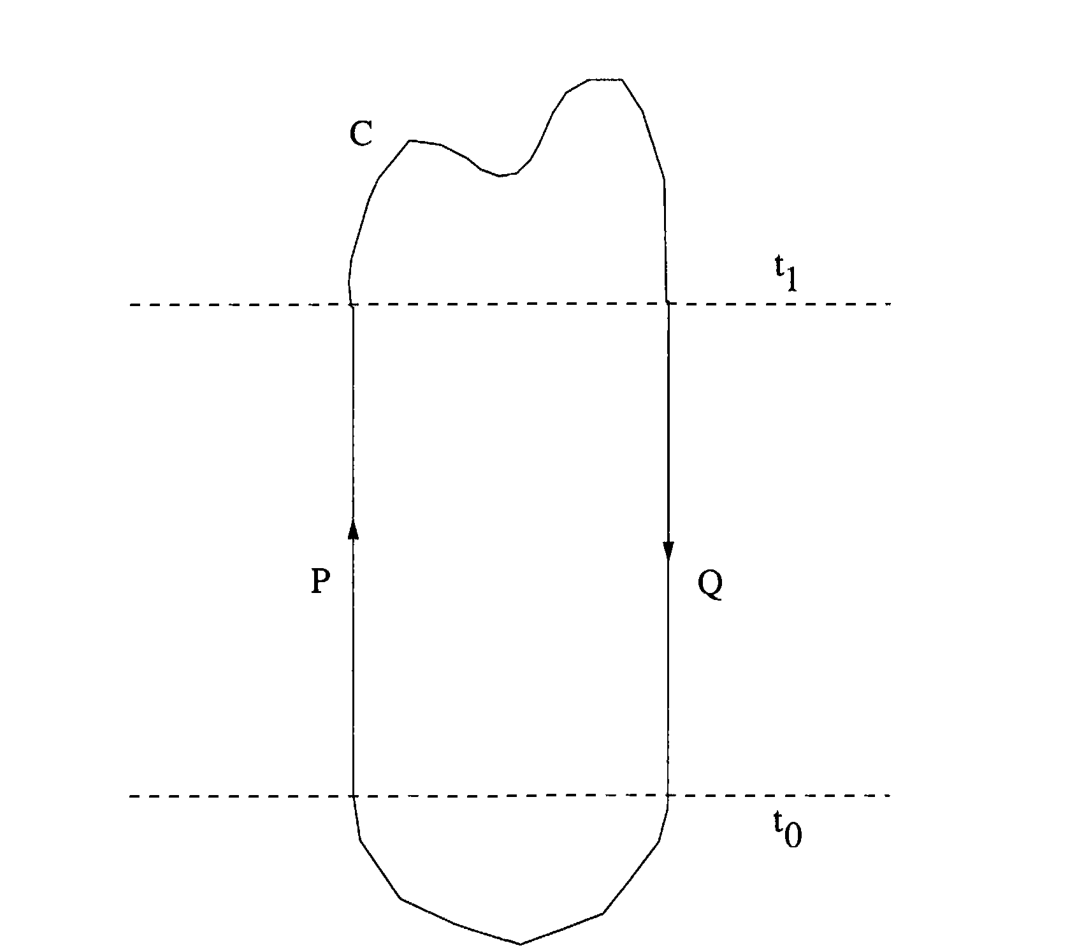
\includegraphics[width=0.52\textwidth]{figs/fig_p099_1.png}
  \caption{Wilson 圈 $C$ 的时空形状示意图。$C$ 在 $t_0<t<t_1$ 之间呈 $P\times\mathbb{R}-Q\times\mathbb{R}$ 的形状（沿 $P$ 一侧向上、沿 $Q$ 一侧向下，箭头表示定向），而在 $t_0$ 之前与 $t_1$ 之后被「封闭」起来；两条虚线是时刻 $t=t_0$ 与 $t=t_1$ 的空间切片。（原文 Figure 1，p.99）}
  \label{fig:p099-1}
\end{figure}

如本页图所示，我们假定：在某个时刻 $t_0$ 之前、以及在某个时刻 $t_1$ 之后，$C$ 并不只是看起来像 $P\times\mathbb{R}-Q\times\mathbb{R}$，而是以某种方式被「封闭」起来（closed off）。$t_0$ 之前的路径积分与 $t_1$ 之后的路径积分分别算出某个初始态与某个末态，记作 $|\psi_i\rangle$ 与 $|\psi_f\rangle$，它们属于 $\mathcal{H}_{P,Q}$。（当然，我们还不知道 $\mathcal{H}_{P,Q}$ 是什么。）从时刻 $t_0$ 到 $t_1$ 的传播给出一个因子 $e^{-iH_{P,Q}(t_1-t_0)}$（若采用欧氏号差（Euclidean signature），则为 $e^{-H_{P,Q}(t_1-t_0)}$）。于是图中 Wilson 线的期望值可以算作
\[
\langle\psi_f|e^{-H_{P,Q}(t_1-t_0)}|\psi_i\rangle .
\]

但 $\mathcal{H}_{P,Q}$ 与 $H_{P,Q}$ 究竟是什么？

首先，如果给定了联络（我们将假定它在 $t_0$ 与 $t_1$ 之间与时间无关），而人们想用刚写下的那类公式来计算 $W_R(C)$，该怎么做？这纯粹是经典数学的问题，并不真正涉及量子场论。人们自然会这样定义 $\mathcal{H}_{P,Q}$：它由 $R\otimes R^*$ 构成（$R^*$ 是 $R$ 的对偶），其中我们认为 $R$「生活」在 $P$ 处、$R^*$「生活」在 $Q$ 处。\footnote{更确切地说，规范场 $A$ 是主丛 $\mathcal{P}$ 上的联络，它在 $P$ 处或 $Q$ 处的纤维我们记作 $\mathcal{P}_P$ 或 $\mathcal{P}_Q$。我们把 $\mathcal{P}_P\times_G R$ 记作 $R$，把 $\mathcal{P}_Q\times_G R^*$ 记作 $R^*$。} 在 $t=t_0$ 之前的「过去」中，从 $Q$ 到 $P$ 的平行移动（parallel transport）决定了 $R\otimes R^*$ 中的一个向量 $|\psi_i\rangle$；同样，在 $t_1$ 之后的「未来」中，从 $P$ 回到 $Q$ 的平行移动给出同一空间中的向量 $|\psi_f\rangle$。现在假定在 $t_0$ 与 $t_1$ 之间联络与时间无关，其含义是：相对于某个平凡化（trivialization），它可以用一个与时间无关的一形式表示。那么我们可以写出
\[
W_R(C)=\langle\psi_f|e^{-iH_{P,Q}(t_1-t_0)}|\psi_i\rangle
\]
其中 $|\psi_i\rangle$ 与 $|\psi_f\rangle$ 就是刚才描述的 $R\otimes R^*$ 中的那两个向量，而 $H_{P,Q}$（它是作用在 $R$ 上的项与作用在 $R^*$ 上的项之和）依赖于 $t_0<t<t_1$ 时那个特定的与时间无关的联络。（事实上，$H_{P,Q}$ 由此联络在「时间」方向上的分量决定。）

因此，若规范场是固定的，则只要取 $\mathcal{H}_{P,Q}=R\otimes R^*$，我们就能得到所需形式的表示。那么，若把规范场按量子力学处理，又当如何？

% [Tutor Note: 这里把与 $R$ 相伴的丛仍记作 $R$、把与 $R^*$ 相伴的丛仍记作 $R^*$，是全文的记号滥用；但真正要留意的是 $P$ 与 $Q$ 两处的因子互为对偶这一点。原因是：在 $t_0<t<t_1$ 区间内，$C$ 沿 $P$ 一侧向上、沿 $Q$ 一侧向下，两段具有相反的定向，故量子化后 $A_0$ 在两因子上的作用相差一个符号，$H_{P,Q}$ 实际为 $A_0^{(R)}\otimes 1-1\otimes A_0^{(R^*)}$ 型的算符；若把两处都取成 $R$（而非 $R^*$），则「时间」方向的相位不会相消，得到的就不是 $\operatorname{Tr}_R$ 沿圈的和乐，而是 $\operatorname{Tr}_R\bigl(\mathrm{Hol}\cdot\mathrm{Hol}\bigr)$ 之类无意义的量。等价的说法是：沿闭合圈定向走一圈时，$R^*$ 上诱导的平行移动是 $R$ 上平行移动之逆。]

% ===== 原文 p.100 =====
我们回忆一下：若把规范场按量子力学处理而不出现 Wilson 线，该怎么做。如上面所述，此时令 $\mathcal{A}$ 为所有联络构成的空间，$\mathcal{H}_0$ 为 $\mathcal{A}$ 上的 $L^2$ 函数构成的空间。然后我们考虑规范群 $\widetilde{G}$ 在 $\mathcal{H}_0$ 上的作用。物理的 Hilbert 空间就是不变元构成的空间 $\mathcal{H}$，即 $\mathcal{H}=\mathcal{H}_0^{\widetilde{G}}$。

显然，我们必须把这两种构造「混合」起来。下述自然的混合方式，可以通过重新审视最初把路径积分与 Hamiltonian 联系起来的那些论证来加以论证。（另一种做法是：我在 §7.7 中勾画了另一条论证下述构造的进路之开端。）我们把 $\mathcal{H}_0$ 替换为 $\mathcal{H}_0\otimes R\otimes R^*$，并定义 $\mathcal{H}_{P,Q}=(\mathcal{H}_0\otimes R\otimes R^*)^{\widetilde{G}}$。至于 Hamiltonian $H_{P,Q}$，它形式上由同一个表达式给出，即
\[
\frac{e^2}{2}\int d^3x\operatorname{Tr}\bigl(-\delta^2/\delta A(x)^2\bigr)+\frac{2}{e^2}\int d^3x\operatorname{Tr}F^2 ,
\]
只不过现在是在 $\mathcal{H}_{P,Q}$ 中求值。

% [Tutor Note: 印出的两项系数不相称：动能项为 $e^2/2$，而磁能项为 $2/e^2$，二者之积恰为 $1$。按 (7.15) 的作用量 $S=\frac{1}{4e^2}\int\operatorname{Tr}F\wedge *F$ 作正则量子化（取 $\operatorname{Tr}T^aT^b=\frac12\delta^{ab}$），对称的标准形式是 $H=\frac{e^2}{2}\int\operatorname{Tr}\Pi_i^2+\frac{1}{2e^2}\int\operatorname{Tr}B_i^2$（$B_i=\frac12\epsilon_{ijk}F_{jk}$，$\Pi_i$ 为 $A_i$ 的共轭动量），两项之积为 $1/4$；印出的 $2/e^2$ 与之差 4 倍（若把 $\operatorname{Tr}$ 换成基础表示的归一化，则差 2 倍）。故此处疑为排印之误，也可能是 $\operatorname{Tr}$ 与 $A$ 采用了另一种归一化。要点在于：$e$ 只以「$e$ 与 $1/e$ 配对」的方式出现——$e\to0$ 时动能项（电场能）趋于零而磁能项发散，这才是下文把 $e$ 当作弱耦合参数的意义所在；切勿用印出的字面系数去核对数值因子。]

更一般地，给定任意一组点 $P_i\in M_s$（$i=1,\dots,n$）以及与之相伴的 $G$ 的表示 $R_i$，我们令 $R_i(P)=\mathcal{P}_{P_i}\times_G R_i$。然后定义 Hilbert 空间
\[
\mathcal{H}_{P_1,R_1;P_2,R_2;\dots;P_n,R_n}=\bigl(\mathcal{H}_0\otimes\textstyle\bigotimes_{i=1}^{n}R_i(P)\bigr)^{\widetilde{G}} .
\]
我们说这就是「在点 $P_i$ 处带有处于表示 $R_i$ 中的外源电荷（external charge）的理论的 Hilbert 空间」。

我们可以把这推广到诸 $P_i$ 的位置随时间变化的情形。例如，让我们回到与一个圆 $C$ 相联系的 Wilson 圈的情形。我们仍假定 $C$ 在点 $P,Q$ 处横截地（transversely）与 $t=0$ 切片相交，但不再假定 $C$ 在 $t=0$ 附近与时间无关。令 $P(t),Q(t)$ 为 $C$ 与给定时刻的切片随时间变化的交点。于是我们必须在随时间变化的 Hilbert 空间族
\[
\mathcal{H}(t)=\bigl(\mathcal{H}_0\otimes R(P(t))\otimes R^*(Q(t))\bigr)^{\widetilde{G}}
\]
中工作，它带有一个随时间变化的 Hamiltonian，并且（我们希望）还带有一个自然的联络。

% [Tutor Note: 上句中 $R_i(P)$ 的括号里写的是 $P$，下标却是 $P_i$，正确记号应为 $R_i(P_i)$；这处不一致在下文 $\mathcal{H}(t)$ 的写法（$R(P(t))$）中才自洽。另需注意：当 $P(t)$ 随时间移动时，$(R(P(t)))^{\widetilde{G}}$ 这类「逐时刻取不变子空间」的做法只有在诸 $R(P(t))$ 之间给定了自然的等变联络（即「随时间变化的 Hilbert 空间族上的联络」）时才有意义——作者自己用 「hopefully」 一词承认这一点尚未建立，这正是他随即转入 §7.7 的动机。]

% 原文 §7.7
\subsection{Wilson 线算符的路径积分表示}

把经典 Wilson 线泛函表示成一维路径积分是方便的。这样的表示将在本节导出。除此以外，这一表示还可以用来把上述对 $\mathcal{H}_{P,Q}$ 的描述之论证纳入一个完全标准的形式。

设 $R$ 是单紧 Lie 群（simple compact Lie group）$G$ 的一个不可约有限维表示。由 Borel–Weil 理论，我们可以把 $R$ 看作 $H^0(G/T,\mathcal{L}_R)$，其中 $\mathcal{L}_R$ 是某个全纯线丛（holomorphic line bundle）。丛 $\mathcal{L}_R$ 带有自然的 Hermitian 度量，因而带有自然的联络 $B$。对任意映射 $\phi:S^1\to G/T$，定义作用量
\[
I_R(\phi)=-\ln\operatorname{Hol}\bigl(\phi^*(B)\bigr)
\]
（Hol 指和乐）。数 $I_R$ 只定义到 $2\pi i n$，但 $e^{-I_R(\phi)}=\operatorname{Hol}(\phi^*(B))$ 是良定义的。

考虑路径积分
\begin{equation}
  \tag{7.10}
  \label{eq:7-10}
  \int D\phi\,e^{-I_R(\phi)} .
\end{equation}
它可以表示成如下形式
\begin{equation}
  \tag{7.11}
  \label{eq:7-11}
  \int D\phi\,e^{i\int_D\phi^*(F_B)} ,
\end{equation}
其中 $F_B$ 是 $B$ 的曲率，$D$ 是以 $S^1$ 的像为边界的圆盘。由这个路径积分定义的量子理论，就是带有零 Hamiltonian 的 Hilbert 空间 $R$（因为该路径积分在微分同胚（diffeomorphism）下不变）。

% ===== 原文 p.101 =====
现在设 $P$ 是圆上某个主 $G$-丛的全空间（total space），带有联络 $A$，并令 $P/T$ 为与之相伴的 $G/T$ 丛。由于 $\mathcal{L}$ 是 $G/T$ 上的 $G$-等变（$G$-equivariant）线丛，它定义了 $P$ 上的一个复线丛，我们把它记作 $\mathcal{L}_P$。$\mathcal{L}$ 上的 Hermitian 联络 $B$ 在竖直方向（沿 $P$ 的纤维）定义了 $\mathcal{L}_P$ 上的一个联络。这个联络可以借助联络 $A$ 自然地延拓为 $\mathcal{L}_P$ 上的联络 $B_P$：在 $P$ 平凡且 $A=0$ 的局部规范中，$B$ 按「常值路径是水平路径」这一条件延拓。

对 $P/T$ 的任意光滑截面（section）$\phi$，定义作用量
\begin{equation}
  \tag{7.12}
  \label{eq:7-12}
  I(\phi,A)=-\ln\operatorname{Hol}\bigl(\phi^*(B_P)\bigr) .
\end{equation}
和以前一样，$I$ 只定义到 $2\pi i n$。

令 $W_R(A)$ 表示 $A$ 沿该圆的和乐在 $R$ 中的迹。现在容易看出，泛函 $W_R(A)$ 有如下积分表示：
\begin{equation}
  \tag{7.13}
  \label{eq:7-13}
  W_R(A)=\int_{\phi\in\Gamma(P/T)}e^{-I(\phi,A)}\,D\phi .
\end{equation}

% [Tutor Note: 「现在容易看出」背后用了三件事：(1) Borel–Weil 定理给出 $H^0(G/T,\mathcal{L}_R)\cong R$，且其余上同调为零（Borel–Weil–Bott），这就是为什么只有不可约表示才出现、且 $\phi$ 的靶空间必须是旗流形 $G/T$；(2) 由 (7.11) 定义的量子理论 Hamiltonian 为零，故它在圆上的配分函数就是其 Hilbert 空间的维数 $\dim R$，插入 $A$ 之后则给出 $\operatorname{Tr}_R$ 的平行移动；(3) $I$ 只在模 $2\pi i$ 的意义下定义，故 $e^{-I}$ 是映射空间 $\Gamma(P/T)$ 上某个线丛的截面，「对 $\phi$ 的积分」严格说是对该线丛截面的积分（需要把 $D\phi$ 的测度与曲率 $F_B$ 一并理解），这也是为何 (7.13) 的右端在 $A$ 作大规范变换下仍良定义。]

现在设 $C$ 是 $M$ 中的一个圈，$A$ 是 $M$ 上主 $G$-丛 $P$ 中的联络。设 $f:S^1\to C$ 是一个参数化。于是有
\begin{equation}
  \tag{7.14}
  \label{eq:7-14}
  W_R(C)(A)=\int_{\phi\in\Gamma(f^*P/T)}e^{-I(\phi,f^*A)}\,D\phi .
\end{equation}

这给出了 Wilson 线算符的一个积分表示。这一表示使我们能把 $C$ 存在时的理论用路径积分表示出来，而这个路径积分完全是标准类型的，只除了一点：某些场遍布整个时空，而 $\phi$ 只在 $C$ 上有定义。例如，在纯规范理论（pure gauge theory）的情形，我们会写
\begin{equation}
  \tag{7.15}
  \label{eq:7-15}
  \int DA\,D\phi\,\exp\Bigl(-\frac{1}{4e^2}\int\operatorname{Tr}F\wedge *F-I(\phi,A|_C)\Bigr) .
\end{equation}

一旦这样做，若再考虑 $C$ 在 $t_0<t<t_1$ 与时间无关的情形，就可以用完全标准的技术引入 Hilbert 空间与 Hamiltonian。沿着这条路走，就能重新得到我先前陈述的对 $\mathcal{H}_{P,Q}$ 的描述。在此请读者把它作为一个练习来思考。基本上，$R$ 与 $R^*$ 来自对 $\phi$ 的量子化，而 $\mathcal{H}_0$ 来自对 $A$ 的量子化；而限制到 $\mathcal{H}_{P,Q}=(\mathcal{H}_0\otimes R\otimes R^*)^{\widetilde{G}}$，正是规范场论中限制到规范不变态的通常做法。

\textbf{评注（Remark）}。注意 (7.13)、(7.14) 的被积函数是一个 Abel 联络的和乐，因此它可以显式地算作曲率积分的指数。这样，我们就把圆上任一线性微分方程的单值（monodromy）表示成了对无穷多个辅助变量（auxiliary variable）的显式积分。经典分析中众所周知：这样的表示若只允许有限多个辅助变量，一般是做不到的；只有某些「超几何」型的特殊方程才可能。

% [Tutor Note: 原文此句作 「This, we have represented the monodromy…」，按文意为 「Thus」，属排印讹误（同页上文刚用过 「This gives an integral representation…」 作句首，疑为串行）。此处的「无穷多个辅助变量」指截面 $\phi$ 在 $C$ 上每一点、每一方向上的取值，即 $\Gamma(f^*P/T)$ 是一个无穷维空间；而「有限多个辅助变量不可能」正是线性微分方程理论中「超几何型方程的和乐构成可约/有限单值群」的另一说法（参见 hypergeometric equation 与 Riemann–Hilbert 问题的经典结果），作者并未在此给出证明，只作类比。]

% ===== 原文 p.102 =====
% 原文 §7.8
\subsection{Higgs 相与禁闭相}

我们现在在欧氏空间（Euclidean space）中工作。考虑一个近似为矩形的 Wilson 圈：两个电荷产生、彼此分开距离 $L$，在该距离上保持时间 $T\gg L$，然后彼此湮灭。（见图。）

\begin{figure}[htbp]
  \centering
  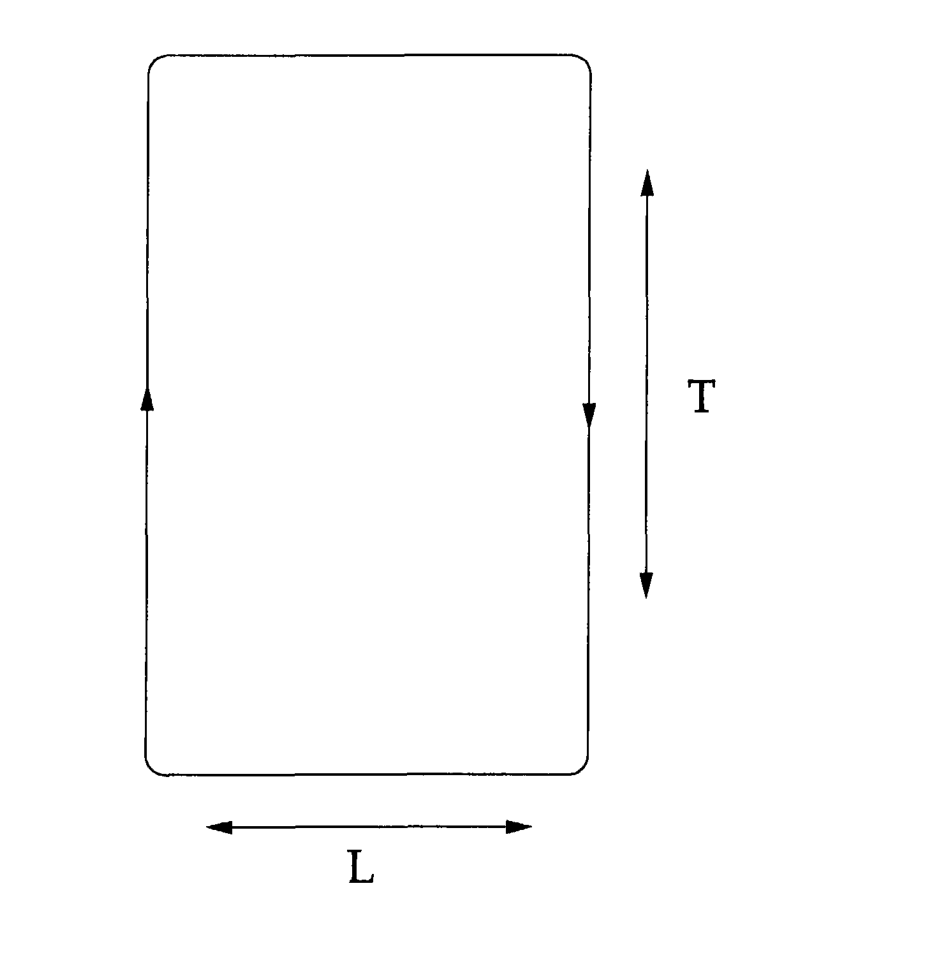
\includegraphics[width=0.42\textwidth]{figs/fig_p102_1.png}
  \caption{近似矩形的 Wilson 圈：纵向箭头标出 $T$（电荷对存在的时间），横向箭头标出 $L$（两电荷之间的距离）；左侧竖边上的箭头向上、右侧竖边上的箭头向下，表示 Wilson 圈的定向。（原文 Figure 1，p.102）}
  \label{fig:p102-1}
\end{figure}

于是 Wilson 圈算符的期望值 $\langle W_R(C)\rangle$（在欧氏框架下）有如下含义：它近似等于 $Ce^{-TV(L)}$，其中 $V(L)$ 是两个电荷在距离 $L$ 处的相互作用能量，而 $C$ 是一个依赖于 $C$ 在初始与末了时刻附近细节形状的常数。更确切地说，$V(L)$ 是 $\mathcal{H}_{P,Q}$ 中的基态能量与通常 Hilbert 空间 $\mathcal{H}$ 中的基态能量之差。关于 Wilson 圈期望值在 $T$ 很大时按 $Ce^{-TV(L)}$ 依赖于 $T$ 的断言，可由上面详细讨论过的它的 Hamiltonian 表示
\[
W_R(C)=\langle\psi_f|e^{-HT}|\psi_i\rangle
\]
推出。

% [Tutor Note: 此处的常数 $C$ 与圈 $C$ 同名，是原文的记号冲突（同一段中 $C$ 既指圈又指常数），阅读时须按上下文区分。另：由 $\langle\psi_f|e^{-HT}|\psi_i\rangle$ 看出，$e^{-TV(L)}$ 这一形式假定了 $T$ 远大于 $\mathcal{H}_{P,Q}$ 中第一激发态能隙的倒数 $\sim1/\Delta E$，从而只有基态存活；并且要求 $|\psi_i\rangle,|\psi_f\rangle$ 在基态上的投影不为零。因为该投影的绝对值被吸收进常数 $C$，所以 $C$ 依赖圈两端（即电荷「产生」与「湮灭」处）的形状，而不依赖 $T$、$L$。顺带一提，$V(L)$ 取的是「两态之「差」」，正是为了让 $V$ 中不含真空能密度这一发散量。]

所以 $\langle W_R(C)\rangle$ 的渐近行为取决于 $V(L)$ 在 $L\to\infty$ 时的渐近行为。物理学家相信，在二维以上具有质量间隙的规范场论中（二维有一些特殊性，其中一些我们稍后会看到），只有两种可能：

\begin{enumerate}
  \item \textbf{Higgs 相（Higgs regime）}：$V(L)\to\mathrm{const}$，$L\to\infty$。
  在这个相中，电荷（其类型见下面的评注）可以以有限的能量代价彼此分开。
  \item \textbf{禁闭相（confinement regime）}：$V(L)\sim\mathrm{const}\cdot L$，$L\to\infty$，其中该常数为正。
  在这个相中电荷被禁闭，不花费任意大的能量就不能彼此分开。
\end{enumerate}

现在让我们考虑任意形状的 Wilson 圈 $C$，其周长为 $S$，其所张成的曲面的极小面积为 $A$。有一个普遍的猜想：在给定质量间隙的前提下，若模式 1 与 2 在 $T\gg L\gg0$ 时成立，则它们对任意 $C$（在各个方向上都很大）以下述形式成立：Higgs 相对应于渐近行为 $\langle W_R(C)\rangle\sim e^{-wS}$（周长律（circumference law）），而禁闭相

% ===== 原文 p.103 =====
对应于渐近行为 $\langle W_R(C)\rangle\sim e^{-wA}$（面积律（area law））。在两种情形中，$w$ 都是正常数。

这一猜想背后的直观是：有了质量间隙，对 Wilson 线的响应或多或少是局域的——在 Higgs 情形中局域在 $C$ 本身上，在禁闭情形中则局域在 $C$ 所张成的极小面积曲面上。极小面积曲面是如何进来的，下周我们讨论 Polyakov 模型时会变得更清楚，随后在第 10 讲讨论 't Hooft 的禁闭图像时也会更清楚。

\textbf{评注 1（Remark 1）}。实际上，只有当 $R$ 是 $G$ 的万有覆盖（universal cover）$\widehat{G}$ 的表示、而不是 $G$ 本身的表示时，禁闭才可能发生。的确，若 $R$ 是 $G$ 的表示，则存在对 $\langle W_R(C)\rangle$ 有贡献的物理过程，其中 Wilson 线的很大一部分电荷为零（即携带 $G$ 的平凡表示），因为理论中某些粒子把 Wilson 线上的电荷湮灭了。这些过程的振幅大于面积律所预言的振幅。重要的是：上面模式 1 与 2 中讨论的「电荷」是借以探测理论的外源电荷——代价是把规范群 $G$ 换成它自己的一个覆盖。它们不是「原来」理论所描述的电荷；在有趣的情形中，它们甚至不像原来理论中的任何电荷那样变换。我们将在下面的玩具例子中说明这一评注。我预计这一评注难以理解，也不指望读者第一遍就能完全弄懂。

\textbf{评注 2（Remark 2）}。上面关于 Higgs 相与禁闭的判据 1 与 2，在其被定义的那类理论中是严格成立的。特别地，我们可以把周长律当作「一个有质量间隙的规范场论处于 Higgs 相」这一说法的精确陈述。这与我们在第 2 讲引入的 Higgs 机制密切相关，但并不总是完全一致。规范对称性破缺的微扰 Higgs 机制是一种在某些弱耦合理论中有用的计算方法。我们没有赋予它在弱耦合之外的意义（这与整体对称性的自发破缺不同——后者我们在第 1 讲给出了公理化的定义），而且即使在 $\pi_1(G)=0$ 时它也完全有意义（在这种情形下，由评注 1，我们目前这一更严格的讨论是空洞的）。相反，Higgs 相的周长律是一条支配某类有质量间隙理论的公理化判据；该判据的陈述与该理论是否有弱耦合描述、或与任何具体的计算方法都无关。按公理化判据处于 Higgs 相的理论，未必能用半经典 Higgs 机制描述（尽管在参数的某个极限下常常可以这样描述）；反之，由半经典 Higgs 机制支配的理论，按公理化判据也不总是处于 Higgs 相（尽管在实践中，当 $\pi_1(G)$ 非平凡时通常如此；事实上主要的反例就是我们即将描述的这个二维例子）。如果刚才这些论断现在显得令人困惑，读者应在进一步学习量子场论之后重新审视它们。

我们其实已经在第 5 讲讨论过禁闭的一个例子。作为另一个略有不同的玩具例子，让我们考虑拉格朗日量为 (7.1) 的二维理论，也就是本讲第一部分研究过的那个理论。此时 $G=U(1)$，其万有覆盖为 $\widehat{G}=\mathbb{R}$。设 $R$ 是 $\widehat{G}$ 的表示，由 $\lambda\in\mathbb{R}:x\mapsto e^{i\lambda x}$ 定义。于是，经典地有 $W_R(C)=e^{i\lambda\int_D F_A}$，其中 $\partial D=C$。

% [Tutor Note: 评注 1 的条件（$R$ 是 $G$ 的万有覆盖 $\widehat{G}$ 的表示而非 $G$ 的表示）与 p.105 猜想的条件（$R$ 不是伴随群 $G_{ad}$ 的表示）看上去互相冲突，实则针对两类不同理论：评注 1 讨论的是「含物质场」的理论，物质场本身取值于 $G$ 的表示，故任何一个 $G$ 的表示（哪怕高维）都可被「成对产生」的物质粒子完全屏蔽，只有不属于 $G$ 的表示（即 $G$ 的覆盖的表示）才无法屏蔽；而 p.105 讨论「纯规范理论」，此时能用来屏蔽的只有伴随表示中的胶子，它们保持电荷的「$N$-ality」不变，故只要 $R$ 不是 $G_{ad}$ 的表示（$N$-ality 非零）就无法屏蔽。对单连通的 $G$（如 $SU(3)$），$\widehat{G}=G$，评注 1 的条件确实空洞，这正是必须换成 $G_{ad}$ 的原因。换言之：评注 1 说的是「物质屏蔽」，猜想说的是「胶子屏蔽」，二者并不矛盾，但绝不可互相替代。]

% ===== 原文 p.104 =====
在量子力学上，我们可以写
\begin{equation}
  \tag{7.16}
  \label{eq:7-16}
  \langle W_R(C)\rangle=\int DA\,D\phi\,D\bar\phi\;e^{-\mathcal{L}}e^{i\lambda\int_D F} .
\end{equation}

% [Tutor Note: (7.16) 的指数写作 $e^{-\mathcal{L}}$，但 $\mathcal{L}$ 在 (7.1) 中是拉格朗日量「密度」，而此处需要的显然是欧氏作用量 $\int d^2x\,\mathcal{L}$（否则量纲与 (7.17) 中对 $V-A_C$、$A_C$ 的面积分解都无法对应）。这是作者一贯的记号滥用：本讲中他用 $\mathcal{L}$ 兼指密度与其积分。同理，$D\bar\phi$ 对应的复标量 $\bar\phi$ 在 (7.15) 中未写出（那里只写了 $D\phi$），因为 (7.15) 讨论的是纯规范理论、$\phi$ 是 Wilson 线的辅助场而非物质场，两者不可混淆。]

设 $V$ 是时空体积，$A_C$ 是 $C$ 所围的面积。我们将把路径积分 (7.16) 拆成两部分的乘积——对 $C$ 内部场取值的积分与对外部取值的积分。由于质量间隙，配分函数近似地分解为「内部」配分函数与「外部」配分函数之积。（还有一个在 $C$ 附近出现的周长修正；它不影响关于面积律的讨论。）注意 (7.16) 中最后一个因子（和乐因子）与 (7.1) 中的拓扑项属于同一类型。因此，(7.16) 给出
\begin{equation}
  \tag{7.17}
  \label{eq:7-17}
  \langle W_R(C)\rangle=\frac{1}{Z}\exp\bigl(-(V-A_C)E(\theta)-A_C E(\theta+2\pi\lambda)\bigr) ,
\end{equation}
略去边界项，我们在此不予考虑。这里 $E(\theta)$ 是作为 $\theta$ 的函数的真空能量密度；它可以用本讲第一部分的方法近似算出。由于在没有 Wilson 圈时配分函数为 $Z=e^{-VE(\theta)}$，我们得到
\begin{equation}
  \tag{7.18}
  \label{eq:7-18}
  \langle W_R(C)\rangle=\exp\bigl(A_C\bigl(E(\theta)-E(\theta+2\pi\lambda)\bigr)\bigr) .
\end{equation}

按照我们的计算，当 $\theta=0$ 时，$E(\theta+\lambda)-E(\theta)$ 化为
\begin{equation}
  \tag{7.19}
  \label{eq:7-19}
  E(\lambda)-E(0)=2(1-\cos2\pi\lambda)e^{-I/e^2}P .
\end{equation}

% [Tutor Note: 正文与 (7.19) 都写作 $E(\theta+\lambda)$、$E(\lambda)$，但按 (7.1) 的拓扑项 $-\frac{i\theta}{2\pi}\int F$，Wilson 圈因子 $e^{i\lambda\int_D F}$ 给出的平移量是 $2\pi\lambda$。用 (7.7) $E_{\rm vac}(\theta)=-P_0-2Pe^{-I}\cos\theta$ 直接验算：$E(2\pi\lambda)-E(0)=2Pe^{-I}(1-\cos2\pi\lambda)$，与 (7.19) 右端相符；而 $E(\lambda)-E(0)$ 只能给出 $1-\cos\lambda$，对不上。故 (7.19) 左端应为 $E(2\pi\lambda)-E(0)$，正文的 $E(\theta+\lambda)$ 应为 $E(\theta+2\pi\lambda)$——两处同样漏写了 $2\pi$；若把 (7.1) 的拓扑项误记成 $i\theta\int F$，则会得出「平移量就是 $\lambda$」的错误结论。(7.19) 中的 $P$ 是单瞬子行列式因子（见 (7.7) 与 §7.5）；另外本讲 (7.7) 写 $e^{-I}$、(7.19) 写 $e^{-I/e^2}$，同一量的两种写法前后不统一，读者应按「瞬子作用量 $=I/e^2$」理解。]

这总是正的，只要 $\lambda$ 不是整数。于是，$\theta=0$ 时的理论 (7.1) 对所有满足「$\lambda$ 不是整数」的外源电荷都表现出禁闭相。$\lambda$ 不为整数这一条件，意思不过是：我们出发时所用的表示是规范群的万有覆盖 $\mathbb{R}$ 的表示，而不是原规范群 $G=U(1)$ 的表示。这与上面的评注 1 一致：按我们所陈述的判据，禁闭只对这样的外源电荷出现——它们表示规范群的一个覆盖，而不表示规范群本身。

因此，尽管这个理论由微扰 Higgs 机制支配，按照上面的公理化判据，它在 $\theta=0$ 时处于禁闭相。所以在这个特例中，微扰 Higgs 机制与 Higgs 相的抽象判据相当不同。在二维以上，人们预期（并且在三维中已证明）这个理论按抽象判据也处于 Higgs 相，同时也表现出微扰 Higgs 机制。

回到二维，人们从上面还会看到：若 $\theta\neq0$，面积律中的系数可以是正的，也可以是负的。这是二维的一个奇特之处：在二维以上，负系数当然是不可预期的。

% 原文 §7.9
\subsection{禁闭猜想}

下面这个猜想在量子场论中是核心的。

% ===== 原文 p.105 =====
\textbf{猜想（Conjecture）}。\textit{设 $G$ 是单紧 Lie 群，$R$ 是 $G$ 的一个表示，且它不是伴随群（adjoint group）$G_{ad}$ 的表示。在 3 维与 4 维中，规范群为 $G$、拉格朗日量为 $\int\operatorname{Tr}(F\wedge *F)$ 的纯规范理论，对取值于 $R$ 的电荷表现出禁闭。在 4 维中，这对 $\theta$ 角的任何值仍然成立。}

这个猜想中与自然界观察到的强相互作用（它们支配核物理以及别的一些东西）相关的情形是 $G=SU(3)$、$R=\mathbb{C}^3$。该猜想的这一特殊情形就意味着夸克（quark）的禁闭。

在二维中，关于纯规范理论的类似陈述在 $\theta=0$ 时为真；这由我们第 5 讲的讨论可以推出。当 $\theta\neq0$ 时，二维的情形更复杂，即使在 Abel 情形中也是如此，正如我们刚刚所见。

\medskip
\noindent\textbf{参考文献与交叉引用（References and cross references）}

二维规范场论在第 5 讲与第 6 讲中讨论。Wilson 线算符以及 3 维、4 维中的禁闭在后面的讲次中讨论，特别是第 8 讲与第 10 讲。


\clearpage
% 原文 pp.107–114（印刷 pp.1225–1232）
\section{Lecture 8：Abel 对偶}

\begin{keytakeaways}
本讲系统讲述二维、三维、四维中的 Abel 对偶（abelian duality）：把取值于圆周 $S^1$ 的标量场（或 $U(1)$ 联络）与另一套自由度互换，使强弱耦合对调。二维情形是半径 $R$ 的圆周上的自由场与半径 $1/R$ 的自由场之间的等价（「$R$ 变成 $1/R$」），推导只用一个 Lagrange 乘子场 $\sigma$ 与 Gauss 积分，却给出配分函数之间的精确关系，其中含与 Euler 示性数有关的因子 $(R/2\pi)^{\chi(\Sigma)}$；同一框架下算符 $d\phi$ 对偶到 $-\frac{i}{R^2}\ast d\sigma$，而顶点算符 $e^{in\phi(P)}$ 对偶到「删去该点、并对具有给定缠绕数的 $\sigma$ 求和」这一非局部处方。三维情形把 $S^1$ 值标量场对偶到规范耦合 $e=\sqrt{\Lambda}$ 的 $U(1)$ 规范场，从而把 Laplace 方程的解与 Maxwell 方程的解对应起来，并把 $e^{in\phi(P)}$ 对应到「在 $P$ 附近第一 Chern 类为 $n$ 的线丛上求和」，这是磁单极子算符的雏形；四维情形则与 $SL(2,\mathbb{Z})$ 有关，将在 Donaldson 理论中使用。作为应用，本讲末尾以三维对偶讨论 Polyakov 的 $SO(3)$ 规范-Higgs 模型，给出二维以上关于禁闭（confinement）现象最具体的可解模型之一。
\end{keytakeaways}

% ===== 原文 p.107 =====
\subsection{引言}
% 原文 §8.1：Introduction

今天，我们将讨论二维、三维与四维中的 Abel 对偶。

在二维，Abel 对偶把圆的半径 $R$ 反演，通常被称为「$R$ 变成 $1/R$」的等价。在某个超对称（supersymmetry）版本中，它导致镜像对称（mirror symmetry）的一个线性版本。

在三维，研究完对偶之后，我们将给出它在 Polyakov 的禁闭（confinement）模型中的一个应用。

四维的 Abel 对偶与一个 $SL(2,\mathbb{Z})$ 对称性有关，我们最终会用它来理解 Donaldson 理论，也就是四维的 $\mathcal{N}=2$ 超对称理论。在此过程中我们会找到另一个禁闭模型。事实上，对偶的这两个应用给出了二维以上已知的、关于禁闭现象的最具体的模型。

我们首先给出对偶的经典表述。在二维，考虑一个含有场 $\phi$、$\sigma$ 的理论，二者都满足 Laplace 方程
\begin{equation}
  \tag{8.1}
  \label{eq:8-1}
  \nabla^2\phi=0;\qquad \nabla^2\sigma=0,
\end{equation}
并通过
\begin{equation}
  \tag{8.2}
  \label{eq:8-2}
  d\phi=\ast d\sigma
\end{equation}
相联系。经典地，这两个场中的任何一个都可以取作该理论的基本场。例如，若我们从满足 $\nabla^2\sigma=\ast d\ast d\sigma=0$ 的 $\sigma$ 出发，则 $d\ast d\sigma=0$，于是局部地可以写下 $\ast d\sigma=d\phi$，其中 $\phi$ 是某个场；也就是说，$\sigma$ 决定了 $\phi$（局部地，且差一个可加常数）。

% [Tutor Note: (8.2) 与四维的 (8.5) 在几何上并不同类：二维欧氏空间中 Hodge 星作用于 1-形式满足 $\ast^2=-1$，故 $d\phi=\ast d\sigma$ 等价于 $d\sigma=-\ast d\phi$，它其实是「闭且余闭的 1-形式局部必为某函数的微分」这一 Hodge 分解的表述，而非自对偶条件；只有在四维，$\ast^2=+1$ 作用于 2-形式，(8.5) $F_A=\ast F_B$ 才有把曲率劈为自对偶/反自对偶部分的意义（这正是 Donaldson 理论的入口）。若把二维的 $\ast^2=-1$ 误记为 $+1$，则 (8.17)→(8.19) 配平方时残留项的符号会整个反过来。]

同样地，在三维，考虑一个含场 $\phi$ 的理论，$\phi$ 满足 Laplace 方程；再考虑某个线丛（line bundle）$\mathcal{L}$ 上的联络 $A$，其曲率 $F=dA$ 满足 Maxwell 方程
\begin{equation}
  \tag{8.3}
  \label{eq:8-3}
  dF=d\ast F=0,
\end{equation}
其对偶关系为
\begin{equation}
  \tag{8.4}
  \label{eq:8-4}
  \ast d\phi=F.
\end{equation}
再次同上，这两个场中的任何一个都可以取作基本场。

% [Tutor Note: (8.3)–(8.4) 的实质是「交换 Bianchi 恒等式与场方程」：给定 $\phi$ 调和，令 $F=\ast d\phi$，则 $dF=dd\phi=0$ 自动成立，而 $d\ast F=\pm d\ast\ast d\phi=\pm dd\phi=0$（三维中 2-形式上 $\ast^2=+1$）；反之，由 $dF=d\ast F=0$ 知 $\ast F$ 闭且余闭，故局部等于 $d\phi$。注意 $F=dA$ 只在 $\mathcal{L}$ 平凡时整体成立，否则 $F$ 只是 $\mathcal{L}$ 的曲率，$\frac{1}{2\pi}\int F$ 为整数（第一 Chern 类）——这一整体性在三维对偶中正是磁单极子荷的来源，参见 (8.30) 之后关于 $H^1(M,\mathbb{R}/\mathbb{Z})$ 的讨论。]

\noindent\textit{（本讲笔记由 David Morrison 整理。）}

% ===== 原文 p.108 =====
在四维，类似物是线丛 $\mathcal{L}_A$ 与 $\mathcal{L}_B$ 上的两个联络 $A$ 与 $B$，二者各自满足 Maxwell 方程，并通过
\begin{equation}
  \tag{8.5}
  \label{eq:8-5}
  F_A=\ast F_B
\end{equation}
相联系。

就 Abel 对偶而言，只要愿意，我们还可以继续走向更高维；但要找到有趣的应用，就得进入弦论。

\subsection{二维对偶}
% 原文 §8.2：Duality in two dimensions

我们想研究这些经典陈述的量子版本。先从二维情形开始。我们把 $S^1$ 等同于 $\mathbb{R}/2\pi\mathbb{Z}$，并在圆上使用加法坐标。取 $\phi$ 为映射 $\phi:\Sigma\to S^1$，其中 $\Sigma$ 是紧致可定向曲面，配有 Riemann 度量 $g_{\alpha\beta}$。（稍后我们会考虑一个变体：在其中 $\phi$ 不要求在若干指定点 $P_i$ 处有定义，也就是说，$\phi$ 将把 $\Sigma-\{P_i\}$ 映入 $S^1$。）我们的拉格朗日量\footnote{本讲所有拉格朗日量都写在欧氏号差（Euclidean signature）下。}为
\begin{equation}
  \tag{8.6}
  \label{eq:8-6}
  \mathcal{L}(\phi)=\frac{R^2}{4\pi}\int d^2x\,\sqrt{g}\,\partial_\alpha\phi\,\partial^\alpha\phi
  =\frac{R^2}{4\pi}\int d\phi\wedge\ast d\phi .
\end{equation}
其运动方程 $dd\phi=d\ast d\phi=0$ 再现了上面讨论的经典理论。

% [Tutor Note: (8.6) 的系数并非任意。把靶空间取为半径 $R$ 的圆、令 $\phi$ 的周期为 $2\pi$，则靶空间度量为 $R^2d\phi^2$，于是 $\mathcal{L}=\frac{R^2}{4\pi}(\partial\phi)^2$ 正是「半径 $R$ 的圆」上的自由场；等价地，令 $\phi=y/R$（$y$ 的周期为 $2\pi R$）即得标准的 $\frac{1}{4\pi}(\partial y)^2$。这也解释了为何对偶理论 (8.21) 的耦合是 $1/R^2$：对偶把靶空间度量取倒数。若把 (8.6) 的 $R^2$ 误当作「$1/g^2$」式的规范耦合，就会把 $R\to1/R$ 误解为一个平凡的重命名，而看不到它交换了「动量模」与「缠绕模」。]

我们将用多种方式研究这个理论。惯用的技巧是：引入新变量，使得把它们积掉（integrate out）会回到原来的理论；然后反过来把旧变量积掉而保留新变量，以便得到该理论的对偶表述。

所以我们实际上要研究另一个理论，它含有场 $\phi$ 与 $A$，其中 $\phi$ 是平凡 $S^1$-丛 $\mathcal{S}$ 的一个截面，$A$ 是 $\mathcal{S}$ 上的一个联络。选取 $\mathcal{S}$ 的一个平凡化 $\phi_0$（于是 $A=\phi_0^\ast\tilde A$，其中 $\tilde A$ 是丛的全空间上的某个 1-形式），我们可以定义协变导数
\begin{equation}
  \tag{8.7}
  \label{eq:8-7}
  D_A\phi=d\phi+A,
\end{equation}
并引入新的拉格朗日量
\begin{equation}
  \tag{8.8}
  \label{eq:8-8}
  \mathcal{L}(\phi,A)=\frac{R^2}{4\pi}\int d^2x\,\sqrt{g}\,(\partial_\alpha\phi+A_\alpha)(\partial^\alpha\phi+A^\alpha)
  =\frac{R^2}{4\pi}\int D_A\phi\wedge\ast D_A\phi .
\end{equation}
虽然令 $A$ 为零即可回到旧的拉格朗日量，但并没有任何机制强制这一点，除非我们再引入第三个场 $\sigma$，让它扮演 Lagrange 乘子（Lagrange multiplier）的角色。我们取 $\sigma$ 为从 $\Sigma$ 到 $S^1$ 的映射，并写下拉格朗日量
\begin{equation}
  \tag{8.9}
  \label{eq:8-9}
  \mathcal{L}(\phi,A,\sigma)=\frac{R^2}{4\pi}\int D_A\phi\wedge\ast D_A\phi-\frac{i}{2\pi}\int\sigma\wedge F_A,
\end{equation}
其中 $F_A$ 是 $A$ 的曲率。

最后这一项需要作些说明。由于我们假定圆丛 $\mathcal{S}$ 是平凡的，可以整体地写出 $F_A=dA$，而最后一项应被理解为 $\frac{i}{2\pi}\int d\sigma\wedge A$（在分部积分之后）；之所以需要这一步，是因为 $\sigma$ 不是单值的。更一般地，即使 $\mathcal{S}$ 非平凡，也可以用一点拓扑来定义这样的项，即定义 $\exp\bigl(\frac{i}{2\pi}\int\sigma\wedge F_A\bigr)$，其做法类似于定义 Chern–Simons 形式。

写下这个拉格朗日量的要点在于：$\mathcal{L}(\phi,A,\sigma)$ 等价于 $\mathcal{L}(\phi)$，下面我们就来证明。一个朴素的分析如下：$\sigma$ 不出现在任何导数中，

% ===== 原文 p.109 =====
而它的运动方程是 $F_A=0$；施加这一条件后，我们就可以走到一个 $A=0$ 的规范，从而回到原来的理论。

更整体地，我们考虑路径积分
\begin{equation}
  \tag{8.10}
  \label{eq:8-10}
  Z=\frac{1}{\mathrm{vol}(G)}\int\mathcal{D}\phi\,\mathcal{D}A\,\mathcal{D}\sigma\,
  \exp\Bigl[-\frac{R^2}{4\pi}\int D_A\phi\wedge\ast D_A\phi+\frac{i}{2\pi}\int\sigma\wedge F_A\Bigr].
\end{equation}
（眼下我们先关注配分函数，但带算符插入的路径积分也可以用同样的方式处理，这一点我们稍后再讨论。）借助标准公式
\begin{equation}
  \tag{8.11}
  \label{eq:8-11}
  \int\frac{dx}{2\pi}\,e^{ixy}=\delta(y),
\end{equation}
我们想说：做完 $\sigma$ 积分就会把 $F_A$ 置零。对这一断言应当谨慎，因为我们研究的是取值于圆周的函数。

% [Tutor Note: (8.11) 只是 $\mathbb{R}$ 上的 $\delta$ 函数表示；而这里 $\sigma$ 取值于圆群 $S^1$，$\int\mathcal{D}\sigma\,e^{\frac{i}{2\pi}\int\sigma\wedge F_A}$ 实际上不是 $\delta(F_A)$，而是「按缠绕数分层求和」之后的 $\delta$ 函数梳——这正是 (8.12) 要写出的内容。换言之 (8.11) 的等式与 (8.10) 之间差着一次对 $d\sigma_h\in H^1(\Sigma,2\pi\mathbb{Z})$ 的求和；若直接把 (8.11) 用在圆值场上，会漏掉 (8.13) 中整个 $\prod_j\sum_{m_j}$ 因子，也就得不到 (8.15) 里第二个 $\delta$ 函数。]

记住我们把 $S^1$ 等同于 $\mathbb{R}/2\pi\mathbb{Z}$，映射 $\sigma:\Sigma\to S^1$ 局部上可以写成一个实值函数，但它未必整体单值；不过 $d\sigma$ 将是 $\Sigma$ 上（单值的）实 1-形式。选取圆周值函数 $\sigma_h:\Sigma\to S^1$，使 $d\sigma_h$ 是 $d\sigma$ 的 de Rham 上同调类中的调和代表元（harmonic representative）。（我们这样规范 $\sigma_h$ 的选取：取定某点 $P\in\Sigma$，并要求 $\sigma_h(P)\in2\pi\mathbb{Z}$。）于是可以写 $\sigma=\sigma_h+\sigma_{\mathbb{R}}$，其中 $\sigma_{\mathbb{R}}$ 是单值实函数。

注意 $\frac{1}{2\pi}d\sigma$，等价地 $\frac{1}{2\pi}d\sigma_h$，必须有整周期。特别地，若取整系数调和 1-形式的一组基 $\lambda_j$，并写 $d\sigma_h=\sum2\pi m_j\lambda_j$，则 $m_j\in\mathbb{Z}$。

现在来计算：
\begin{align}
  \tag{8.12}
  \label{eq:8-12}
  \int\mathcal{D}\sigma\,e^{\frac{i}{2\pi}\int\sigma\wedge F_A}
  &=\int\mathcal{D}\sigma_{\mathbb{R}}\,e^{\frac{i}{2\pi}\int\sigma_{\mathbb{R}}\wedge F_A}
  \sum_{d\sigma_h\in H^1(\Sigma,2\pi\mathbb{Z})}e^{-\frac{i}{2\pi}\int d\sigma_h\wedge A}\\
  \tag{8.13}
  \label{eq:8-13}
  &=\delta(F_A)\prod_j\Bigl(\sum_{m_j\in\mathbb{Z}}e^{-im_j\int\lambda_j\wedge A}\Bigr).
\end{align}

第一个因子告诉我们 $A$ 是平坦联络（flat connection）。此外，在平坦联络之中，规范等价类 $[A]$ 由和乐（holonomy）标记，等价地由量 $\int\lambda_j\wedge A$ 标记。由于被积函数的其余部分规范不变，我们可以规范固定（略去因子 $(\mathrm{vol}(G))^{-1}$），并在规范等价类的空间上积分（这是一个有限维积分）：
\begin{align}
  \tag{8.14}
  \label{eq:8-14}
  Z&=\int\mathcal{D}\phi\,\mathcal{D}[A]\,e^{-\frac{R^2}{4\pi}\int D_A\phi\wedge\ast D_A\phi}\delta(F_A)
  \prod_j\Bigl(\sum_{m_j\in\mathbb{Z}}e^{-im_j\int\lambda_j\wedge A}\Bigr)\\
  \tag{8.15}
  \label{eq:8-15}
  &=\int\mathcal{D}\phi\,e^{-\frac{R^2}{4\pi}\int D_A\phi\wedge\ast D_A\phi}\delta(F_A)\,
  \delta\Bigl(\int\lambda_i\wedge A=0\quad\mathrm{mod}\ 2\pi\mathbb{Z}\Bigr).
\end{align}

% [Tutor Note: (8.12)→(8.13) 是格上的 Poisson 求和（等价于圆群上的 Fourier 变换）：对缠绕数分层求和后，$\int\mathcal{D}\sigma_{\mathbb{R}}$ 给出 $\delta(F_A)$，而对 $d\sigma_h$ 的和给出环面 $H^1(\Sigma,\mathbb{R})/H^1(\Sigma,2\pi\mathbb{Z})$ 上的 $\delta$ 函数梳，即 (8.15) 中第二个 $\delta$。作者只说「现在来计算」。技术上有两点须留意：其一，$\lambda_j$ 必须是整系数调和 1-形式的基（使 $\int_\Sigma\lambda_i\wedge\lambda_j$ 为交截数矩阵），否则「周期为 $2\pi$ 的整数倍」无从谈起；其二，$\sum_{m_j\in\mathbb{Z}}e^{-im_j\int\lambda_j\wedge A}$ 在 $\int\lambda_j\wedge A\equiv0\ (2\pi)$ 处发散，故它只在该超曲面上有支撑，写成一个 $\delta$ 是形式上的简写。]

于是出现了把和乐与曲率同时置零的 $\delta$ 函数。所以 $A$ 在模规范变换的意义下为零，而我们这个新理论确实等价于原来的理论，其配分函数为
\begin{equation}
  \tag{8.16}
  \label{eq:8-16}
  Z=\int\mathcal{D}\phi\,\exp\Bigl(-\frac{R^2}{4\pi}\int d\phi\wedge\ast d\phi\Bigr).
\end{equation}

现在让我们以相反的次序积分，即积掉 $\phi$ 与 $A$ 而保留 $\sigma$。为积掉 $\phi$，我们这样规范固定：使 $\phi=0$，

% ===== 原文 p.110 =====
并从而在路径积分中略去因子 $(\mathrm{vol}(G))^{-1}$。于是路径积分 (8.10) 约化为
\begin{equation}
  \tag{8.17}
  \label{eq:8-17}
  \int\mathcal{D}A\,\mathcal{D}\sigma\,\exp\Bigl[-\frac{R^2}{4\pi}\int A\wedge\ast A+\frac{i}{2\pi}\int\sigma\wedge F_A\Bigr].
\end{equation}
你也许会乐于验证：与这一规范固定相应的 Faddeev–Popov 行列式是
\begin{equation}
  \tag{8.18}
  \label{eq:8-18}
  \int\mathcal{D}c\,\mathcal{D}\bar c\,\exp\Bigl[-\frac{R^2}{4\pi}\int d^2x\,\bar c\,c\Bigr].
\end{equation}

% [Tutor Note: 规范固定 $\phi=0$（即把 $\phi\to\phi+\epsilon$ 的平移对称固定掉）给出的 Faddeev–Popov 算符是 $d:\Omega^0\to\Omega^1$，其行列式为 $(\det\Delta_0)^{1/2}$。作者把它写成 $\int\mathcal{D}c\,\mathcal{D}\bar c\,e^{-\frac{R^2}{4\pi}\int\bar cc}$，并在脚注 2 中特意声明「把 $c$ 看作 0-形式、$\bar c$ 看作 2-形式」：这不是文字游戏，而是因为二维 Hodge 分解给出 $\det\Delta_1=\det\Delta_0\det\Delta_2$（略去调和模），只有按 $0$-形式与 $2$-形式（各 $n_0=n_2$ 个模）来计数，鬼场因子才能与下面 $A'$ 的高斯积分逐项配对，从而产生 (8.20) 中的指数 $(-n_0+n_1-n_2)$。]

为对 $A$ 积分，我们需要配方（complete the square），把指数中的第二项看作 $-\frac{i}{2\pi}\int A\wedge d\sigma$，也就是说，它是 $A$ 的线性项。我们作变量替换 $A'=A+\frac{i}{R^2}\ast d\sigma$；结果（包含 Faddeev–Popov 积分）为
\begin{equation}
  \tag{8.19}
  \label{eq:8-19}
  \Bigl(\int\mathcal{D}c\,\mathcal{D}\bar c\,e^{-\frac{R^2}{4\pi}\int d^2x\,\bar c\,c}\Bigr)
  \Bigl(\int\mathcal{D}A'\,e^{-\frac{R^2}{4\pi}\int A'\wedge\ast A'}\Bigr)
  \Bigl(\int\mathcal{D}\sigma\,e^{-\frac{1}{4\pi R^2}\int d\sigma\wedge\ast d\sigma}\Bigr).
\end{equation}
（对 $A'$ 的 Gauss 积分，如同 Faddeev–Popov 行列式，可以看作归一化因子。）

% [Tutor Note: 这一步的平移是「虚平移」：$A'=A+\frac{i}{R^2}\ast d\sigma$ 中的 $i$ 意味着 $A$ 被解析延拓为复值联络，否则线性项 $-\frac{i}{2\pi}\int A\wedge d\sigma$ 不能被实平移消掉。按标准 Gauss 积分 $\int dA\,e^{-aA^2+bA}\propto e^{b^2/4a}$ 逐项验算：$a=\frac{R^2}{4\pi}$、$b=-\frac{i}{2\pi}$（线性项耦合的是 $\ast d\sigma$，而 $A\wedge\ast(\ast d\sigma)=-A\wedge d\sigma$ 用到二维 1-形式上 $\ast\ast=-1$），于是 $b^2/4a=+\frac{1}{4\pi R^2}$。若把 $A$ 当作实场，残留项就是正的，对偶理论看似发散；而 (8.19) 给出的负号只能来自 $A$ 积分轮廓的转动（等价于 $A\to iA$），即作者写下 (8.17) 时已默认联络复化。取使对偶作用量负定、积分收敛的那一支，与 (8.21) 的最终结果自洽。符号若不追到轮廓这一步，最容易得出「对偶理论发散」的错误结论。]

Faddeev–Popov 积分对 $\Sigma$ 上每个 0-形式与每个 2-形式各给出一个因子 $\bigl(\int dt\,e^{-tR^2/4\pi}\bigr)^{-1}$\footnote{为此，请把 $c$ 看作一个 0-形式、把 $\bar c$ 看作一个 2-形式。}；对 $A'$ 的积分对 $\Sigma$ 上每个 1-形式给出一个因子 $\int dt\,e^{-tR^2/4\pi}$。于是，若以 $n_j$ 记「$\Sigma$ 上 $j$-形式的个数」，这些项合起来给出总的因子
\begin{equation}
  \tag{8.20}
  \label{eq:8-20}
  \bigl(\sqrt{\pi}/(R^2/4\pi)\bigr)^{(-n_0+n_1-n_2)}=(R/2\pi)^{\chi(\Sigma)}.
\end{equation}

% [Tutor Note: 这里 (8.20) 左右两端按字面并不相等，是原书的一处笔误：以 $a=R^2/4\pi$ 记之，$\int dt\,e^{-ta}=\sqrt{\pi/a}$，故每个 0-形式与 2-形式贡献 $(\sqrt{\pi/a})^{-1}$、每个 1-形式贡献 $(\sqrt{\pi/a})^{+1}$，总因子应为 $\bigl(\sqrt{\pi}/\sqrt{R^2/4\pi}\bigr)^{(-n_0+n_1-n_2)}=(2\pi/R)^{(-n_0+n_1-n_2)}$；再用 $\chi(\Sigma)=2-2g=n_0-n_1+n_2$ 即得右端的 $(R/2\pi)^{\chi(\Sigma)}$。原书分母上的根号漏掉了（或等价地指数应减半），若照抄则两端相差 $(R/2\pi)^{2\chi}$。此处照原样译出，读者引用时请以右端为准。]

也就是说，联系这两个对偶表述的变换规则是
\begin{equation}
  \tag{8.21}
  \label{eq:8-21}
  \int\mathcal{D}\phi\,\exp\Bigl[-\frac{R^2}{4\pi}\int d\phi\wedge\ast d\phi\Bigr]
  =(R/2\pi)^{\chi(\Sigma)}\int\mathcal{D}\sigma\,\exp\Bigl[-\frac{1}{4\pi R^2}\int d\sigma\wedge\ast d\sigma\Bigr].
\end{equation}
（因子 $(R/2\pi)^{\chi(\Sigma)}$ 没有出现在今年其他讲者所作的具体计算中，因为他们的计算是在亏格 1 的情形做的。）第一个理论中的耦合 $R$ 映到第二个理论中的耦合 $1/R$，这就是为什么这个对偶有时被称为「$R$ 变成 $1/R$」。

% [Tutor Note: $(R/2\pi)^{\chi(\Sigma)}$ 是配分函数在 $R\to1/R$ 下的「反常」：$R$ 同时出现在作用量系数与测度归一化中，二者并不抵消。亏格 1 时 $\chi=0$、因子为 $1$，这正是作者说其他讲者在环面上的显式计算看不到它的原因；一般亏格下它必须用 $\zeta$ 函数正规化的行列式比值来定义，属于 $c=1$ 紧致玻色子的标准结果（可与 Polchinski 关于圆上玻色子 $T$-对偶的讨论对勘）。]

现在我们想追踪这个理论中的算符在对偶变换下的像，并确定它对关联函数以及配分函数的影响。一个容易的情形是 $d\phi$，我们预期它映到 $\ast d\sigma$，正如经典理论中那样（实际上，把归一化考虑进去后，它会映到 $\ast d\sigma$ 的一个倍数）。我们需要把上述计算重复一遍，但插入一些算符 $\prod_i\mathcal{O}_i(\phi)$，其中之一是 $d\phi$。为此，我们需要 $d\phi$ 的一个规范不变的扩充，而协变导数正好提供了它：
\begin{equation}
  \tag{8.22}
  \label{eq:8-22}
  d\phi(x)\ \bigl(\text{第一个理论}\bigr)\ \longrightarrow\ D_A\phi(x)\ \bigl(\text{大理论}\bigr).
\end{equation}
然后容易验证：当我们积掉 $\sigma$（并把 $A$ 规范固定为零）时，它映回 $d\phi$。

一般地，映射算符的困难之处在于：要为给定的算符找到它在更大的理论中的恰当扩充，

% ===== 原文 p.111 =====
而这个扩充在积掉 $\sigma$ 之后要回到原来的算符。对 $d\phi$ 来说这并不太难，正如我们刚刚看到的。

当路径积分中插入了 $D_A\phi$ 时，我们的计算会怎样改变？先前配方时，我们作了变量替换 $A'=A+\frac{i}{R^2}\ast d\sigma$。如果路径积分中已插入 $D_A\phi$，那么经过这一变量替换，它变为 $D_{A'}\phi-\frac{i}{R^2}\ast d\sigma$。在推导的其余部分，当 $\phi$ 被规范固定为零、$A'$ 被积掉之后，我们剩下的就是在对偶理论中插入 $-\frac{i}{R^2}\ast d\sigma$。因此，这就是 $d\phi$ 在对偶理论中的像。

在操作这些算符插入之间的映射时，必须小心。例如，尽管 $d\phi$ 映到 $-\frac{i}{R^2}\ast d\sigma$，但局部算符 $(d\phi)^2$ 在对偶理论中并不会映到 $\bigl(\frac{i}{R^2}\ast d\sigma\bigr)^2$，原因是在配方时引入了非线性。

% [Tutor Note: 这一段点出对偶的一个根本限制：只有「线性于导数」的算符有局部而简单的像。$d\phi\to D_A\phi$ 之所以干净，是因为 $D_A\phi=d\phi+A$ 与 $A$ 线性耦合，而 $A$ 的平移是常数平移；一旦算符含 $(D_A\phi)^2$，平移后会出现 $D_{A'}\phi$ 与 $\frac{i}{R^2}\ast d\sigma$ 的交叉项，它不与 $\sigma$ 解耦，于是像算符变成非局部的。等价地说，$R\to1/R$ 不是场空间之间的逐点映射，而是算符代数之间的同构，只在某些「顶点算符」上保持局部性——这正是下面要引入非局部对象 (8.23) 的动机。]

使这个情形容易的原因在于，协变导数是通常导数的一个自然的规范不变扩充。

更难对付的算符插入是 $e^{i\phi}$。它没有规范不变的版本。另一方面，我们其实并不需要它，因为 $\langle e^{i\phi(P)}\rangle=0$。但两点关联函数 $\langle e^{i\phi(P)}e^{-i\phi(Q)}\rangle$ 一般不为零，所以当 $P\ne Q$ 时，我们应当设法对这样的插入作对偶化。

我们要做一件相当奇怪的事。对这一对算符插入，不可能构造出局部的规范不变扩充；因此我们在对偶过程中（也就是说，在中间那个理论中）非局部地处理它，在路径积分中引入如下形式的项
\begin{equation}
  \tag{8.23}
  \label{eq:8-23}
  e^{i\phi(P)}e^{-i\phi(Q)}e^{\frac{i}{2\pi}\int\theta\wedge A},
\end{equation}
其中 $\theta$ 是 1-形式，满足
\begin{equation}
  \tag{8.24}
  \label{eq:8-24}
  \frac{1}{2\pi}d\theta=\delta_P-\delta_Q,
\end{equation}
且 $\theta$ 的所有周期在模 $2\pi\mathbb{Z}$ 的意义下为零。

% [Tutor Note: (8.24) 有解的前提是 $\delta_P-\delta_Q$ 作为分布是恰当形式，即 $P-Q$ 作为 0-链在 $H_0(\Sigma)$ 中为零；两个同次数的 0-链之差总是边缘，所以 $\theta$ 总存在——这就是「两点函数可以沿一条割线局域化」的拓扑根据。条件「所有周期 $\equiv0\ (2\pi\mathbb{Z})$」保证 $e^{\frac{i}{2\pi}\int\theta\wedge A}$ 不依赖于 $\theta$ 的选取；而 (8.25) 的规范不变性可直接验证：在 $A\to A+d\epsilon$ 下 $e^{i\int_\ell A}\to e^{i\int_\ell A}e^{i(\epsilon(Q)-\epsilon(P))}$，恰被 $e^{i\phi(P)}e^{-i\phi(Q)}$ 在 $\phi\to\phi-\epsilon$ 下的变换抵消。]

为找到这样的 $\theta$，取一条从 $P$ 到 $Q$ 的路径 $\ell$，并令 $\theta/2\pi$ 为 $\ell$ 的 Poincaré 对偶（把 $\ell$ 看作分布）。于是我们可以把我们的项 (8.23) 改写为
\begin{equation}
  \tag{8.25}
  \label{eq:8-25}
  e^{i\phi(P)}e^{i\int_\ell A}e^{-i\phi(Q)},
\end{equation}
这显然是规范不变的表达式。（这是 $\theta$ 的一种选法，但我们允许比这更一般的 $\theta'$。）最终我们会把 $\theta$ 看作 $\Sigma-P-Q$ 上平凡 $S^1$-丛上的一个联络形式。

这样，我们就找到了一个规范不变的非局部对象 (8.23)。假设我们试着把它插入路径积分。首先，若令 $A=0$，我们就回到原来的算符插入 $e^{i\phi(P)}e^{-i\phi(Q)}$，所以我们的确把这对算符正确地扩充到了规范理论。

若要以另一种方式积分，我们把 $\phi$ 规范固定为零，这就把 (8.23) 约化为 $e^{\frac{i}{2\pi}\int\theta\wedge A}$。这是路径积分指数中 $A$ 的线性项的一个新贡献，形式为 $-\frac{i}{2\pi}\int A\wedge\theta$；于是为配方，我们现在必须作变量替换 $A'=A+\frac{i}{R^2}\ast(d\sigma+\theta)$，这使我们的对偶路径积分取形式
\begin{equation}
  \tag{8.26}
  \label{eq:8-26}
  \int\mathcal{D}\sigma\,\exp\Bigl[-\frac{1}{4\pi R^2}\int(d\sigma+\theta)\wedge\ast(d\sigma+\theta)\Bigr].
\end{equation}
也就是说，我们得到了与先前相同的理论，但这时它建立在 $\Sigma-P-Q$ 上，而且这时的路径积分是对映入 $S^1$、且不能延拓

% ===== 原文 p.112 =====
过 $P$ 或 $Q$ 的映射进行的。也就是说，我们写 $\tilde\sigma=\sigma+\alpha$，其中 $d\alpha=\theta$，$\alpha$ 是从 $\Sigma-P-Q$ 到 $S^1$ 的映射；于是 $\tilde\sigma$ 是从 $\Sigma-P-Q$ 到 $S^1$ 的映射，它不能延拓过 $P$ 或 $Q$。事实上，它绕 $P$ 与 $Q$ 的缠绕数（winding number）分别为 $1$ 与 $-1$。

当然，引入 $\tilde\sigma$ 的要点在于：用 $\tilde\sigma$ 写出来，拉格朗日量就只是通常的 $(1/4\pi R^2)\int d\tilde\sigma\wedge\ast d\tilde\sigma$。因此，算符 $e^{i\phi(P)}e^{-i\phi(Q)}$ 的插入，给出了一个场 $\tilde\sigma$ 的通常拉格朗日量，而该场绕 $P$ 或 $Q$ 的缠绕数为 $1$ 或 $-1$。

\begin{figure}[htbp]
  \centering
  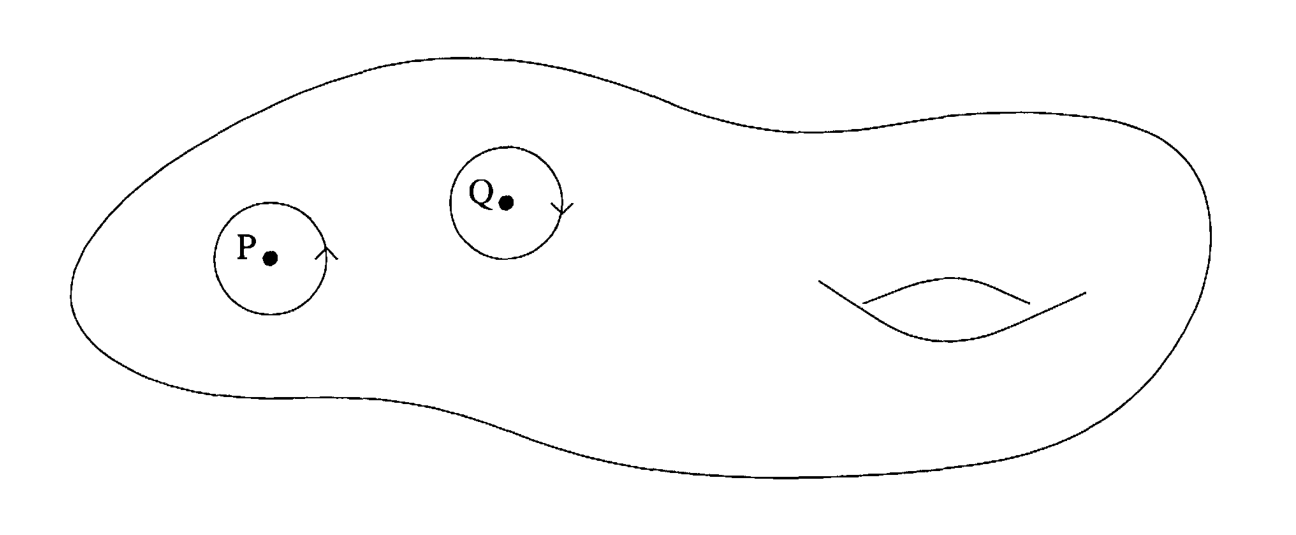
\includegraphics[width=0.62\textwidth]{figs/fig_p112_1.png}
  \caption{带两个穿刺点 $P$、$Q$ 的曲面 $\Sigma$：$P$、$Q$ 各被一个小圆标出，表示 $\tilde\sigma$ 的相位割线（箭头指示绕行方向，绕行一周相位增加 $\pm2\pi$）；右侧的弧线示意 $\Sigma$ 的亏格（把手）。（原文 Figure 1，p.112）}
  \label{fig:p112-1}
\end{figure}

% [Tutor Note: $\tilde\sigma$ 的缠绕数取 $+1,-1$ 由 (8.24) 的归一化决定：$\frac{1}{2\pi}\int_{\text{绕}P\text{的小圆}}d\theta=1$，故 $\frac{1}{2\pi}\oint d\alpha=+1$，即 $\alpha$ 绕 $P$ 一周增加 $2\pi$；绕 $Q$ 时因 $\delta_P-\delta_Q$ 的符号相反而得 $-1$。这也说明 (8.26) 中的 $\theta$ 不能随手扔掉：把它吸收进 $\tilde\sigma$ 之后，$\tilde\sigma$ 已不再是 $\Sigma$ 上的映射，而是 $\Sigma-P-Q$ 上的多值映射，路径积分要在「不能延拓过 $P,Q$ 的映射」这一类上进行。图中 $P$、$Q$ 处的小圈正是这一割线的位置。]

现在有两类算符：一类在其中一个图像中是局部的，另一类在另一个图像中是局部的。算符 $e^{in\phi(P)}$（在第一种描述中）被映到另一种描述中的一条指令：「把 $P$ 从 $\Sigma$ 上删去，并对绕 $P$ 缠绕数为 $n$ 的 $\sigma$ 作路径积分」。反过来，第二种描述中的普通局部算符 $e^{in\sigma}(P)$，在第一种描述中对应一条非局部的处方。

\subsection{三维对偶}
% 原文 §8.3：Duality in three dimensions

现在转向三维理论。先考察一个 $S^1$ 值函数 $\phi$ 在（固定的）紧致三维流形 $M$（可以带边界）上的理论，其拉格朗日量为
\begin{equation}
  \tag{8.27}
  \label{eq:8-27}
  \mathcal{L}=\frac{\Lambda}{4\pi}\int d^3x\,\sqrt{g}\,\partial_\alpha\phi\,\partial^\alpha\phi
  =\frac{\Lambda}{4\pi}\int d\phi\wedge\ast d\phi .
\end{equation}
三维的一个新奇之处是：前因子 $\Lambda$ 具有质量的量纲。由于 $\Lambda$ 是带量纲的量而非常数，在 $\Lambda$ 取某个数值时不可能发生任何特殊的事情。

我们把理论推广到 $\phi$ 是平凡 $S^1$-丛 $\mathcal{L}_B$ 的截面、并带有联络 $B$ 的情形，写下包含协变导数 $D_B\phi=d\phi+B$ 的拉格朗日量：
\begin{equation}
  \tag{8.28}
  \label{eq:8-28}
  \mathcal{L}(\phi,B)=\frac{\Lambda}{4\pi}\int d^3x\,(\partial_\alpha\phi+B_\alpha)(\partial^\alpha\phi+B^\alpha)
  =\frac{\Lambda}{4\pi}\int D_B\phi\wedge\ast D_B\phi
\end{equation}
如果把它当作一个自成体系的理论、把 $B$ 与 $\phi$ 都当作量子场，那么它是一个相当平庸的理论；经典运动方程告诉我们，在差一个规范变换的意义下一切都是零，量子理论同样平庸。为了有所进展，我们引入一个带有联络 $A$ 的线丛 $\mathcal{L}$，以及拉格朗日量
\begin{equation}
  \tag{8.29}
  \label{eq:8-29}
  \mathcal{L}(\phi,B,A)=\frac{\Lambda}{4\pi}\int D_B\phi\wedge\ast D_B\phi-\frac{i}{2\pi}\int A\wedge F_B,
\end{equation}

% ===== 原文 p.113 =====
把最后一项理解为 $-\frac{i}{2\pi}\int F_A\wedge B$（在分部积分之后）；这样做是合理的，因为 $\mathcal{L}_B$ 平凡，而且在给定平凡化之后，$B$ 就只是一个 1-形式。当 $\mathcal{L}_B$ 非平凡时，其推广是路径积分中的一个因子 $e^{\frac{i}{2\pi}\int A\wedge F_B}$，我们把其中的指数解释为丛 $\mathcal{L}\oplus\mathcal{L}_B$ 上联络 $A\oplus B$ 的 Chern–Simons 不变量。这个因子是良定义的，因为 Chern–Simons 不变量给出到 $\mathbb{R}/2\pi\mathbb{Z}$ 的良定义映射。

为了执行对偶变换，我们需要对线丛 $\mathcal{L}$ 求和，从而得到一个路径积分
\begin{equation}
  \tag{8.30}
  \label{eq:8-30}
  \frac{1}{\mathrm{vol}(G)\mathrm{vol}(G')}\sum_{\mathcal{L}}\int\mathcal{D}\phi\,\mathcal{D}A\,\mathcal{D}B\,
  \exp\Bigl[-\frac{\Lambda}{4\pi}\int D_B\phi\wedge\ast D_B\phi+\frac{i}{2\pi}\int F_A\wedge B\Bigr],
\end{equation}
其中 $G$ 与 $G'$ 分别是 $\mathcal{L}$ 与 $\mathcal{L}_B$ 的规范群。

我们想积掉 $A$。粗略的说法是：这样做会给出 $\delta(F_B)$，从而意味着 $B$ 是平坦联络。正如我们在二维所作的计算那样，复杂性来自 $B$ 具有非平凡和乐的可能性。事实上，若 $F_B=0$，我们可以把 $B$ 看作 $H^1(M,\mathbb{R}/\mathbb{Z})$ 的一个元素，并对每个 $x=c_1(\mathcal{L})$ 定义量 $e^{2\int x\wedge[B]}$。当对 $A$ 作路径积分时对 $[x]$ 求和，结果就是 $\delta([B])$，这表明 $B$ 与平凡平坦联络规范等价。于是我们回到原来的理论；我们已经看到，带有 $A$ 与 $\mathcal{L}$ 的扩充理论等价于原来的理论。

现在我们从相反的方向作积分，即作 $\phi$ 与 $A$ 的积分。如同二维情形，我们通过规范变换把 $\phi$ 置零，从而去掉归一化因子 $(\mathrm{vol}(G))^{-1}$。（与二维不同，Faddeev–Popov 行列式不贡献任何有趣的东西，所以我们不显式写出它。）在所得的路径积分中可以配方：
\begin{align}
  \tag{8.31}
  \label{eq:8-31}
  \frac{1}{\mathrm{vol}(G')}\sum_{\mathcal{L}}\int\mathcal{D}A\,\mathcal{D}B\,
  &\exp\Bigl[-\frac{\Lambda}{4\pi}\int B\wedge\ast B+\frac{i}{2\pi}\int B\wedge F_A\Bigr]\\
  \tag{8.32}
  \label{eq:8-32}
  =\frac{1}{\mathrm{vol}(G')}\sum_{\mathcal{L}}\int\mathcal{D}A\,\mathcal{D}B'\,
  &\exp\Bigl[-\frac{\Lambda}{4\pi}\int B'\wedge\ast B'-\frac{1}{4\pi\Lambda}\int F_A\wedge\ast F_A\Bigr],
\end{align}
其中我们作了平移 $B'=B-\frac{i}{\Lambda}\ast F_A$。对 $B'$ 的积分是 Gauss 型的，可以并进路径积分的归一化，于是剩下
\begin{equation}
  \tag{8.33}
  \label{eq:8-33}
  \frac{1}{\mathrm{vol}(G')}\sum_{\mathcal{L}}\int\mathcal{D}A\,\exp\Bigl[-\frac{1}{4\pi\Lambda}\int F_A\wedge\ast F_A\Bigr],
\end{equation}
这正是 Abel 规范理论中那个熟悉的路径积分，规范耦合为 $e=\sqrt{\Lambda}$。

% [Tutor Note: (8.31)→(8.32) 的配方有两处容易漏掉的技术点。其一，三维中 $F_A\wedge F_A$ 是 4-形式，恒等于零，所以配方后不会留下 $\int F\wedge F$ 型拓扑项；若照搬到四维，就会出现 $\frac{\theta}{8\pi^2}\int F\wedge F$ 那样的项，那正是四维 $SL(2,\mathbb{Z})$ 对偶与 $\theta$ 角的来源。其二，$B$ 与 $F_A$ 的缩并要用三维的 $\ast^2=+1$（1-形式、2-形式皆然，与二维 1-形式上的 $\ast^2=-1$ 相反），据此 $B'=B-\frac{i}{\Lambda}\ast F_A$ 才消去交叉项并留下 $-\frac{1}{4\pi\Lambda}\int F_A\wedge\ast F_A$；若符号弄错会得到 $+\frac{1}{4\pi\Lambda}$，与 (8.33) 所要求的正定 $U(1)$ 作用量不符。读者可用同法逐项核对二维 (8.19) 与三维 (8.32) 两处配方的符号。]

现在我们要映射算符。与二维所作类似的计算表明：$d\phi$ 在更大的理论中扩充为协变导数 $D_B\phi=d\phi+B$，而在对偶理论中变为 $\frac{i}{\Lambda}\ast F_A$。这就是 Laplace 方程的解与 Maxwell 方程的解之间的对偶在量子理论中的含义。

那么 $e^{in\phi(P)}$ 这样的算符呢？这个我们不去做，但我会陈述答案：$e^{in\phi(P)}$ 在对偶的规范理论中被映到如下指令：把点 $P$ 从三维流形 $M$ 上删去，并考虑线丛 $\mathcal{L}$ 上联络的路径积分，其中 $\mathcal{L}$ 的第一 Chern 类在一个小

% ===== 原文 p.114 =====
球面（围绕 $P$）上取值 $n$。导致这一点的论证与我们在二维所做的基本一致。

我不打算给出那个论证（我把它推荐为一道练习），而是讨论大致相反的方向。我们考虑规范理论中的 Wilson 圈（Wilson loop）算符，并试着把它们映回标量场论。

设 $C$ 是 $M$ 中一个作为边界的圆，$\lambda\in\mathbb{R}$。规范理论中有算符 $\exp(i\lambda\oint_C A)$。我们把它插入大理论（即拉格朗日量为 $\mathcal{L}(\phi,B,A)$ 的那个理论）的路径积分。（更一般地，即使 $C$ 不是边界我们也可以这样做，但那时 $\lambda$ 必须限制为整数。设 $C$ 是某个二维曲面 $D$ 的边界，则可写 $\exp(i\lambda\oint_C A)=\exp(i\lambda\int_D F)$，这表明对任意 $\lambda$ 都规范不变。）

当我们在路径积分中带上这个额外因子去积掉 $A$ 时，得到的不是 $\delta(F_B=0)$，而是 $\delta(F_B=2\pi\lambda[C])$，其中 $[C]$ 是 $C$ 的 Poincaré 对偶。换言之，作 $A$ 积分把 $B$ 确定为满足 $F_B=2\pi\lambda[C]$，而积掉 $A$ 之后修改过的拉格朗日量是 $\int D_B\phi\wedge\ast D_B\phi$。这里 $B$ 是平坦的 $U(1)$ 联络，绕该圆有单值性（monodromy）$e^{2\pi i\lambda}$。于是，圆 $C$ 上的 Wilson 圈算符对偶于如下处方：「删去 $C$，并把 $\phi$ 解释为平坦圆丛的一个截面，其绕 $C$ 的加法单值性为 $2\pi\lambda$。」换句话说，我们修改 $\phi$ 为 $\tilde\phi$，使得 $d\tilde\phi=d\phi+B$，并把 $\tilde\phi$ 解释为 $M-C$ 上平凡 $S^1$-丛的一个截面，带有绕 $C$ 的单值性为 $e^{2\pi i\lambda}$ 的平坦联络。（要得到这样一个平凡 $S^1$-丛，我们或者需要假定 $C$ 是边界，或者需要 $\lambda$ 是整数。一切都自洽，因为这些也正是我们出发时的 Wilson 线为规范不变的条件。）

% [Tutor Note: $\delta(F_B=2\pi\lambda[C])$ 中的 $2\pi$ 必须与 (8.29) 的 $\frac{i}{2\pi}\int A\wedge F_B$ 的归一化配套：插入 $e^{i\lambda\oint A}=e^{i\lambda\int_D F}$ 相当于给 $A$ 的线性项加上 $i\lambda\int A\wedge\cdots$，对 $A$ 变分即得 $F_B=2\pi\lambda[C]$，于是 $\oint_C B=2\pi\lambda$、单值性为 $e^{2\pi i\lambda}$。若 $C$ 不是边界而 $\lambda\notin\mathbb{Z}$，$\oint A$ 本身无定义（须先取平凡化），这就是作者强调「$C$ 是边界、或 $\lambda$ 为整数」的原因——它也是 Dirac 量子化条件在三维的翻版：磁单极子（此处即 $A$ 的第一 Chern 类非零的构型）的荷必须量子化。]

\subsection{应用于 Polyakov 模型}
% 原文 §8.4：Application to the Polyakov model

我们将描述一个 Polyakov 大约在 1975 年构造的模型。这是对偶在一个非线性相对论性理论中的首次使用。该模型展示了被称为禁闭的现象。

我们在三维工作，研究带有标量场 $s$（属于三维表示）的 $SO(3)$ 规范理论，其拉格朗日量为
\begin{equation}
  \tag{8.34}
  \label{eq:8-34}
  \mathcal{L}=\frac{1}{4\pi e^2}\int d^3x\,\mathrm{Tr}\,|F|^2
  +\int d^3x\,(D\vec s)^2+\int d^3x\,\lambda(\vec s^{\,2}-a^2)^2 .
\end{equation}
这个模型在树图阶（tree level）展示了 Higgs 机制。

经典地，通过一个规范变换可以把真空转到
\begin{equation}
  \tag{8.35}
  \label{eq:8-35}
  \langle\vec s\rangle=\begin{pmatrix}a<本地路径>
\end{equation}
在真空态中，拉格朗日量的 $SO(3)$ 对称性破缺为 $SO(2)=U(1)$ 对称性，唯一的无质量场是 $U(1)$ 联络。（这就是所谓的 Higgs 机制。）低能理论看起来就像三维的 $U(1)$ 理论。

\textbf{第一步（First Step）.} 在低能下，这个理论经典地看起来像拉格朗日量为
\begin{equation}
  \tag{8.36}
  \label{eq:8-36}
  \mathcal{L}=\frac{1}{4e^2}\int F\wedge\ast F
\end{equation}
的 $U(1)$ 规范理论。

这就是答案吗？自由 $U(1)$ 理论的高斯不动点（Gaussian fixed point）稳定吗？

% [Tutor Note: 对照 (8.34) 与 (8.36)：前者为 $\frac{1}{4\pi e^2}\int\mathrm{Tr}|F|^2$，后者为 $\frac{1}{4e^2}\int F\wedge\ast F$，两处系数相差一个 $\pi$。这不一定是笔误——$\mathrm{Tr}$ 在伴随表示上的归一化、以及 $F\wedge\ast F=|F|^2d^3x$ 的约定都可以吸收常数——但读者若要把 (8.36) 的低能有效耦合与 (8.34) 的树图耦合直接比较（例如估算 Higgs 机制给出的规范场质量 $m\sim ea$ 与低能耦合 $e$ 的关系），必须先统一两处的归一化，否则会整体差出 $\sqrt{\pi}$。]

% 原文 pp.115–121（印刷 pp.1233–1239）

% ===== 原文 p.115 =====
% 原文 §8.4（续）：Polyakov 模型的应用

不稳定性的一个可能来源是 Chern--Simons 相互作用
\begin{equation}
  \tag{8.37}
  \label{eq:8-37}
  \frac{-in}{2\pi}\int A\wedge F_A
\end{equation}
它可以加到原来的拉氏量 $\mathcal{L}$ 上。
若 $A$ 的维数为 $1/2$，则自由理论 (8.36) 是共形不变的，于是 Chern--Simons 相互作用的维数为二，因而是一个相关微扰（relevant perturbation）。
（加上 Chern--Simons 相互作用之后，拉氏量仍然是二次的。一个直接的练习——见秋季学期的作业题 FP4——表明：含该项的拉氏量描述的是一个自由的有质量理论。）

Chern--Simons 项要成为我们问题中不稳定性的来源，有两个障碍。
第一个障碍是：Chern--Simons 项中的系数 $n$ 必须是整数。
这意味着，即使你只能近似地计算这个理论，只要近似可以做得任意精确，你就能确定 $n$。
特别地，人们可以在微扰论中计算 $n$；而由于高圈项会含有 $e$ 的正幂次，它只可能来自单圈项。
因此，\emph{任何}三维规范理论中的有效 $n$ 都可以通过一次显式的单圈计算来确定。
在我们此处所考虑的具体例子中，只需注意到：Chern--Simons 项在宇称（parity）下是奇的（也就是说，它依赖于三维流形定向的选取），而我们的原理论并不如此。
宇称不变性是一圈行列式的一个对称性（无论宇称在低能下最终是否自发破缺），它保证 $n=0$。

% [Tutor Note: 这段论证靠"整性 + 解析性"两步配合，作者都写得很简。(i) 由于 $n$ 必须取整数值，它作为 $e$ 的函数不可能是连续的，故不可能是 $e$ 的非平凡函数——只能是常数；(ii) 另一方面，按 $e$ 的幂次展开时，相对 Chern--Simons 项而言 $L$ 圈（$L\ge2$）的贡献带有 $e^{2L-2}$ 的因子，在 $e\to0$ 时全部消失，于是唯一可能与 $e$ 无关的贡献来自一圈项。两步合起来即得"$n$ 等于它的单圈值"。其次，这里"维数为二"是就拉氏量\emph{密度}而言：三维中边际算符的密度维数为三，$2<3$ 故为相关算符；不要误以为 $\int A\wedge F$ 本身是某个无量纲的作用量。最后，"宇称保持 $\Rightarrow n=0$"只对纯规范理论（或宇称不变的物态）成立：若理论含手征费米子，一圈图会生成 Chern--Simons 项，$n=0$ 的结论即失效——这正是三维 Chern--Simons 物质理论中"宇称反常"的来源。]

在三维的 $U(1)$ 规范理论中，再也写不出别的相关相互作用；因此，任何能使这个理论变得不稳定的东西，都很难用 $A$ 来描述。
然而我们已看到，这个 $U(1)$ 规范理论等价（对偶）于一个标量理论
\begin{equation}
  \tag{8.38}
  \label{eq:8-38}
  \mathcal{L}=\frac{e^2}{4\pi}\int d^3x\,\partial_\alpha\phi\,\partial^\alpha\phi .
\end{equation}
在这个理论中，我们可以加上一项
\begin{equation}
  \tag{8.39}
  \label{eq:8-39}
  g\int d^3x\,\cos n\phi
\end{equation}
（对某个 $n$）。
我们之所以把势取为周期的，是因为 $\phi$ 实际上是一个到圆周的映射。
注意：$g\ne0$ 的理论有质量间隙（mass gap），而 $g=0$ 的理论没有。
于是我们指认出了某种定性地改变物理的东西，但它只能借助对偶变量才能方便地解释。
这很奇怪，因为要做对偶，本来就必须先走到低能描述中去！

这个效应在原初的 $SO(3)$ 理论中会出现吗？
我们先问：它在微扰论中会出现吗？
考虑 $SO(3)$ 理论的 Feynman 图。
我们用波浪线表示无质量模式，用实线表示有质量模式。
一个典型的 Feynman 图，例如

\begin{figure}[htbp]
  \centering
  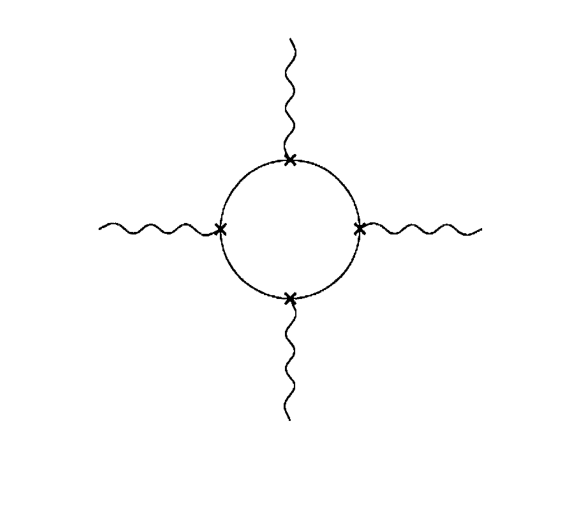
\includegraphics[width=0.34\textwidth]{figs/fig_p115_1.png}
  \caption{一个典型的单圈 Feynman 图：外线为波浪线，表示无质量模式；中间的圆圈为实线，表示有质量模式；叉号标记四个顶点。（原文图示，p.115）}
  \label{fig:p115-1}
\end{figure}

% [Tutor Note: (8.38) 的系数与后面的 (8.49)、(8.50)、(8.53)、(8.54)、(8.56) 不一致，几乎可以肯定是原文的一处笔误，正确值应为 $\frac{1}{4\pi e^{2}}$。两条独立的判据。(i) 拓扑/几何判据：三维中 Hodge $\ast$ 在二形式上是等距同构，且 $F=\ast d\phi$（作者在 p.119 明写此式），故 $F\wedge\ast F=d\phi\wedge\ast d\phi$ 逐点相等，标量理论动能项的系数必须与规范理论动能项 $\frac{1}{4\pi e^{2}}\int F\wedge\ast F$ 完全相同；而 (8.38) 印作 $\frac{e^{2}}{4\pi}$，恰好把 $e^{2}$ 从分母挪到了分子。(ii) 物理判据（更有说服力）：若动能系数为 $\kappa$，则 $\langle F F\rangle\propto\frac{1}{\kappa}\frac{1}{|x|^{3}}$，要与 (8.42) 的 $\frac{e^{2}}{|x|^{3}}$ 相符必须 $\kappa\propto\frac{1}{e^{2}}$。也就是说对偶把强弱耦合互换（$e\to1/e$），这正是三维阿贝尔对偶的标志性特征；反之，若取 (8.38) 的 $\kappa\propto e^{2}$，则 $e\ll1$（瞬子气体稀疏）时 $\phi$ 反而强耦合，p.121 上对 $\phi$ 作半经典（极小曲面）分析就完全不成立了。故 (8.38) 应读作 $\frac{1}{4\pi e^{2}}$。]

% ===== 原文 p.116 =====
这样的图将完全是温和的（tame）：我们有有质量的传播子，它们在低动量处关于动量是解析的。
这类图只是给出 $U(1)$ 规范场 $A$ 的有效作用量的修正，而这些修正可以写成拉氏量中额外的局域、规范不变的项。

\subsection{三维 $SO(3)$ 规范理论中的瞬子}
% 原文 §8.4（续）：instantons

我们需要一种完全不同的东西：\emph{瞬子}（instantons）。
让我们在 $\mathbb{R}^3$ 上工作。
我们在 $\mathbb{R}^3$ 上有一个 $SO(3)$ 丛，其结构群在无穷远处已被约化为 $U(1)$。
在无穷远处的 $S^2$ 上，一个 $U(1)$ 丛 $\mathcal{L}$ 可以有非平凡的第一 Chern 类，$c_1(\mathcal{L})\ne0$。

由于 $\mathbb{R}^3$ 是可缩的，$\mathbb{R}^3$ 上的 $SO(3)$ 丛是平凡的。
取该 $SO(3)$ 丛的一个平凡化，于是我们可以把空间 $\mathbb{R}^3$ 与丛 $\mathbb{R}^3$ 等同起来，并简单地把我们的截面 $s$ 当作一个映射 $s:\mathbb{R}^3\to\mathbb{R}^3$。
为了构造这样的、在无穷远处的 $S^2$ 上具有非平凡拓扑的映射，我们取 $s$ 形如
\begin{equation}
  \tag{8.40}
  \label{eq:8-40}
  s(\vec x)=a\,\frac{\vec x}{|x|}\,f(|x|),
\end{equation}
其中 $f(|x|)$ 是满足 $f(0)=0$、$\lim_{|x|\to\infty}f(|x|)=a$ 的递增函数，例如

\begin{figure}[htbp]
  \centering
  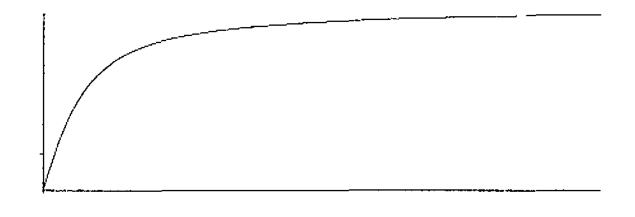
\includegraphics[width=0.52\textwidth]{figs/fig_p116_1.png}
  \caption{剖面函数 $f(|x|)$ 的图形：在原点取值为零，随 $|x|$ 单调递增，并在 $|x|\to\infty$ 时趋于常数 $a$。（原文图示，p.116）}
  \label{fig:p116-1}
\end{figure}

这样的截面在空间转动与规范转动的联合作用下不变。

我们想要这一等价类中作用量极小的解 $s$。
它应当是球对称的，渐近行为是：当 $|x|\to\infty$ 时 $Ds\sim\frac{1}{|x|^2}$。
这导致一个常微分方程，而它有唯一解。
作用量可以写成 $I/e^2$（对某个常数 $I$），因此当耦合趋于零时它发散。

注意，由于 $\vec s$ 恰好在原点处为零，结构群在原点之外被约化为 $U(1)$，但这一约化不能延拓到原点之上。
事实上，在围绕原点的球面上，该线丛具有非零的第一 Chern 类（若在 $SO(3)$ 中工作，它实际上是 $2$；也就是说，$SO(3)$ 的伴随丛在围绕原点的二维球面上分解为
\[
\mathcal{O}\oplus\mathcal{L}\oplus\mathcal{L}^{-1},
\]
其中 $\mathcal{L}$ 的次数为 $2$）。

% [Tutor Note: "次数为 $2$"是本节后面 Remark（p.120–121）的全部要害所在，作者在此只是提前使用。缘由是 $SO(3)=SU(2)/\mathbb{Z}_2$：伴随丛 $\mathcal{O}\oplus\mathcal{L}\oplus\mathcal{L}^{-1}$ 来自 $SU(2)$ 伴随丛（即三矢量表示）的分解，而在 $SU(2)$ 的语言里电荷是以 $\mathcal{L}^{1/2}$ 为基本单位的，故 $SO(3)$ 视角下的线丛是它的平方，$\deg\mathcal{L}=2\deg\mathcal{L}^{1/2}$，必为偶数；等价地说，$w_2$ 是 $c_1\bmod 2$ 的像，而 $w_2=0$ 迫使 $c_1$ 为偶。这也解释了为什么由瞬子诱导的势取 $\cos 2\phi$ 的形式（见 (8.49)、(8.54)），而不是 $\cos\phi$：写 $\cos\phi$ 会在 $\phi\to\phi+\pi$ 下变号，破坏后面要用的对称性。]

从这个观点看，一个纯粹的 $U(1)$ 理论与一个只在长距离上看起来像 $U(1)$ 的理论之间的区别在于：后者可以容许这样的丛，它们在无穷远处的大 $S^2$ 上具有非零的第一 Chern 类。
这个 Chern 类可以是我们在刚刚描述的具体解中所找到的 $2$ 的任意整数倍。

注意，在阿贝尔规范理论中，不可能使用这样的丛 $\mathcal{L}$：它在围绕原点的球面上 $c_1(\mathcal{L})\ne0$，因为这样的丛不能延拓到 $\mathbb{R}^3$ 上。
破缺到 $U(1)$ 的 $SO(3)$ 理论与 $U(1)$ 理论之间的定性差别就在于：前者允许奇点，而 $U(1)$ 描述正是在这种奇点处失效。

如果我们在 $3+1$ 维中做类似的事情，我们会得到一个能量有限（而不是作用量有限）的、与时间无关的解。
这个解看起来像坐在那里的一颗粒子，而事实上它就是一个磁单极子（magnetic monopole）。
（非零的磁荷来自 $c_1(\mathcal{L})\ne0$ 这一事实：它意味着磁场在无穷远处球面上的积分为非零值。）
作这个类比的要点在于：我们可以把瞬子设想为行为如同磁单极子的一个「零时切片」。

% ===== 原文 p.117 =====
瞬子在长距离上看起来是什么样子的？
磁单极子有一个行为如下的场
\begin{equation}
  \tag{8.41}
  \label{eq:8-41}
  F=\mathrm{const}\,\frac{\vec x}{|x|^3}=\mathrm{const}\,\frac{\hat x}{|x|^2}
\end{equation}
（由 Maxwell 方程）。

每个瞬子对路径积分的贡献是\footnote{我们用「$e$」表示规范耦合，这是阿贝尔规范理论中的标准记号。不要把它与自然对数的底「$e$」相混淆。} $e^{-I/e^2}$，当 $e$ 很小时它极其微小。

回到我们的理论，我们现在问：它在长距离上行为如何？
例如，两点函数 $\langle F(x)F(0)\rangle$ 当 $|x|\to\infty$ 时行为如何？

在自由理论中，由量纲分析，答案是 $1/|x|^3$。
（只要考虑拉氏量中的基本项 $\frac{1}{4\pi e^2}\int F\wedge\ast F$，就可以看出三维理论中曲率 $F$ 的维数为 $3/2$。）
更精确一点，我们断言
\begin{equation}
  \tag{8.42}
  \label{eq:8-42}
  \langle F_{ij}(x)F_{k\ell}(0)\rangle=\frac{e^2}{|x|^3}\left(\delta_{ik}\delta_{j\ell}+\dots\right).
\end{equation}

Feynman 图不影响这一渐近行为：$e^2$、等价地说 $1/|x|^3$ 的系数，只有很小的重整化，此外还有一些在大距离上不重要的修正。

瞬子如何影响这一分析？
考虑一个定域在 $y$ 附近的瞬子，以及它对 $x$ 与 $0$ 之间两点函数的影响。

\begin{figure}[htbp]
  \centering
  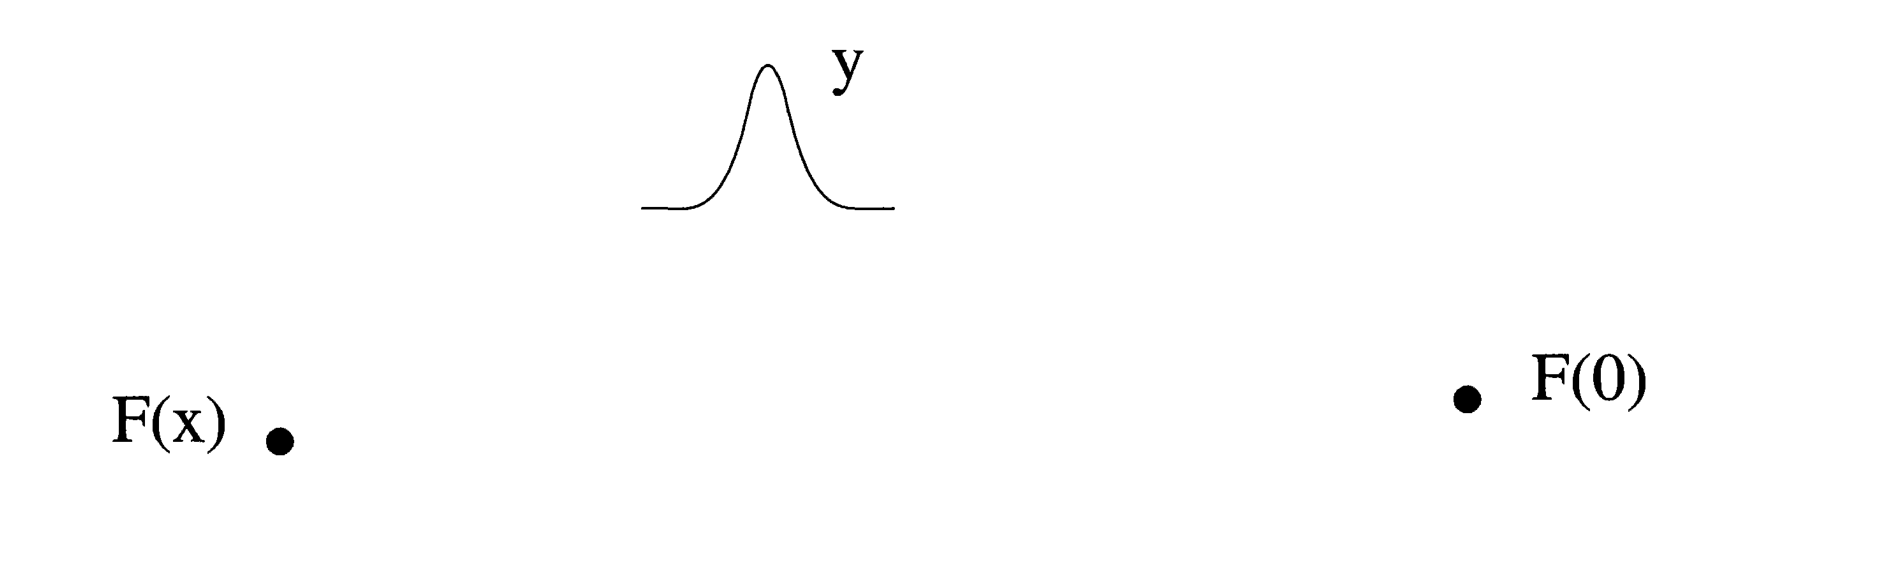
\includegraphics[width=0.66\textwidth]{figs/fig_p117_1.png}
  \caption{定域在 $y$ 附近的瞬子对两点函数 $\langle F(x)F(0)\rangle$ 的贡献示意：钟形曲线表示瞬子场强的空间分布（其峰在 $y$ 处），下方两个黑点分别标记算符插入点 $x$ 与 $0$。（原文图示，p.117）}
  \label{fig:p117-1}
\end{figure}

瞬子扇区中路径积分的首项近似是
\begin{equation}
  \tag{8.43}
  \label{eq:8-43}
  e^{-I/e^2}\int d^3y\,\frac{(\vec x-\vec y)}{|x-y|^3}\,\frac{\vec y}{|y|^3}.
\end{equation}

这里我们对瞬子的位置 $y$ 积分；被积函数就是 $F(x)F(0)$ 在瞬子场中的经典值。
我们把瞬子的经典作用量记作 $I/e^2$，并在对瞬子位置的积分中带上因子 $\exp(-I/e^2)$，因为这是存在一个瞬子的单位体积概率。
（当 $e\to0$ 时 $I$ 与 $e$ 无关。）
该积分按 $1/|x|$ 标度。
因此，把微扰贡献与瞬子修正相加，总的行为是
\begin{equation}
  \tag{8.44}
  \label{eq:8-44}
  \langle F(\vec x)F(\vec 0)\rangle\cong\frac{1}{Z}\Bigl(\text{pert. theory}+e^{-I/e^2}(\text{instanton sector})\Bigr)
\end{equation}
\begin{equation}
  \tag{8.45}
  \label{eq:8-45}
  \cong\frac{1}{Z}\left((1+\dots)\frac{1}{|x|^3}+e^{-I/e^2}\Bigl(\frac{1}{|x|}+\dots\Bigr)\right).
\end{equation}

% [Tutor Note: 作者说 (8.43) "按 $1/|x|$ 标度"，这一步跳过了一个容易忽略的细节：$\int d^3y\,\frac{1}{|x-y|^3}\frac{1}{|y|^3}$ 在 $y\to0$ 处是\emph{对数发散}的（$\frac{d^3y}{|y|^3}\sim\frac{dy}{y}$），在 $y\to\infty$ 处则收敛。故所谓 $1/|x|$ 只是首项标度，真实的积分还要乘一个 $\ln(\text{瞬子尺度}/|x|)$ 型的对数因子，截断尺度由瞬子的大小（即经典解的芯）给出。这也提醒：把瞬子当作点荷来处理，在 $y$ 靠近 $x$ 或 $0$ 时是不成立的，(8.43) 的被积函数在这些区域本应换成瞬子解的真实场强。]

% ===== 原文 p.118 =====
由于瞬子贡献在红外比自由理论项更重要（$1/|x|$ 对 $1/|x|^3$），瞬子引发了一个不稳定性。

为了更细致地看清红外到底发生了什么，我们首先注意到：瞬子是\emph{稀少}的。
在小体积 $V_0$ 中存在一个瞬子的概率正比于 $V_0e^{-I/e^2}$，故每个瞬子所对应的空间体积为 $V\sim e^{I/e^2}$，而两个瞬子之间的空间间距为
\[
R\sim V^{1/3}\sim e^{I/3e^2}.
\]

然而在红外，如果我们考虑足够大的空间体积，就会得到大量的瞬子，可以把它们当作由确定大小的粒子组成的气体。
这些粒子是\emph{带电}的，所以我们不能忽略它们之间由 Coulomb 势给出的相互作用。
图像如下：

\begin{figure}[htbp]
  \centering
  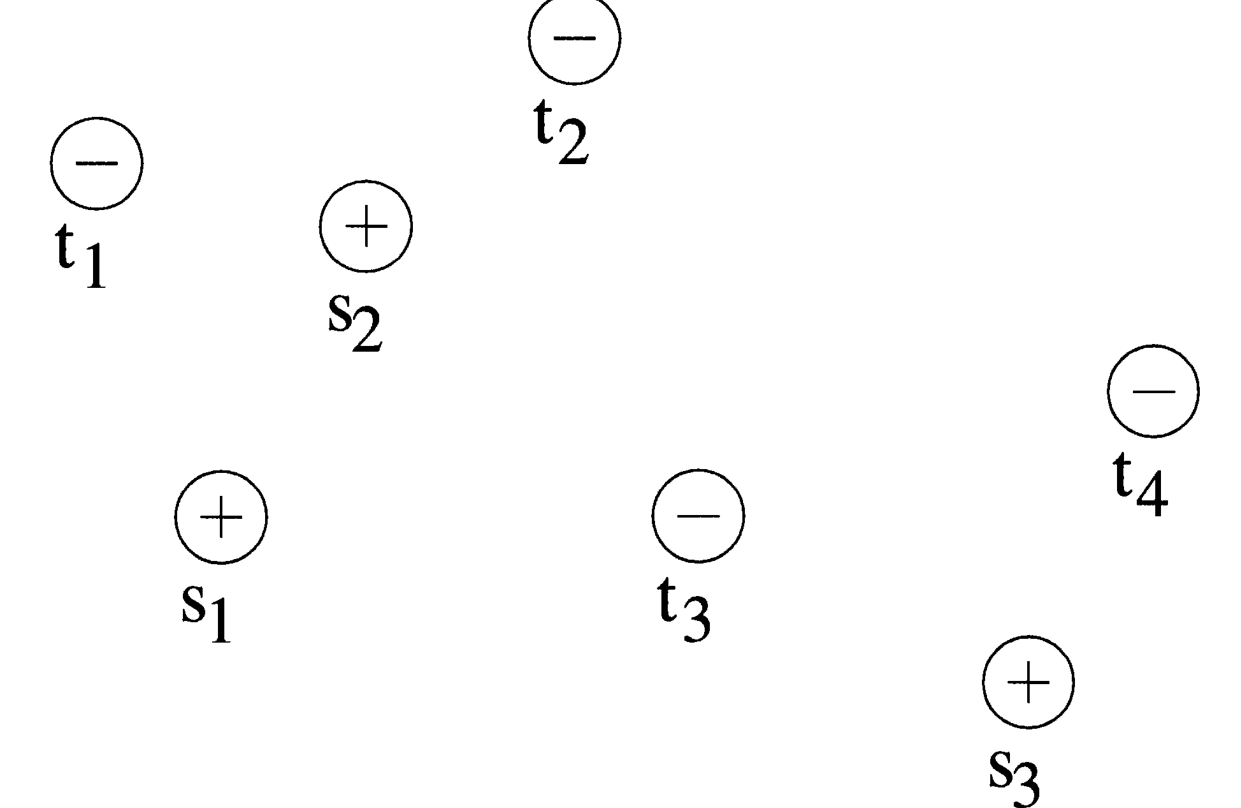
\includegraphics[width=0.52\textwidth]{figs/fig_p118_1.png}
  \caption{三维空间中的瞬子气体：标有 $+$ 的圆圈表示带正荷的瞬子，位置记为 $s_i$；标有 $-$ 的圆圈表示带负荷的反瞬子，位置记为 $t_j$。（原文图示，p.118）}
  \label{fig:p118-1}
\end{figure}

我们用 $s_i$ 标记瞬子（带正荷）的位置，用 $t_j$ 标记反瞬子（带负荷）的位置。
对所有这些求和得到
\begin{align}
  \sum_{n,m=0}^{\infty}\frac{1}{n!m!}&\int d^3s_i\big|_{i=1}^{n}\int d^3t_j\big|_{j=1}^{m}\exp\left(-\frac{I}{e^2}(n+m)\right)\notag\\
  \tag{8.46}
  \label{eq:8-46}
  &\times\exp\left(\frac{1}{4\pi e^2}\sum_{i<j}\left(\frac{1}{|s_i-s_j|}+\frac{1}{|t_i-t_j|}\right)-\frac{1}{4\pi e^2}\sum_{i,j}\frac{1}{|s_i-t_j|}\right).
\end{align}

在被积函数中，我们写出了一个位形的作用量的指数，该位形由位于点 $s_i$ 的彼此远离的瞬子与位于点 $t_j$ 的反瞬子组成。
作用量中的主要项就是 $(n+m)I$，如同瞬子与反瞬子之间没有相互作用。
但此外还有一个相互作用势
\begin{equation}
  \tag{8.47}
  \label{eq:8-47}
  \frac{1}{4\pi e^2}\,\frac{1}{|s_i-s_j|}
\end{equation}
作用在位于 $s_i$、$s_j$ 的瞬子之间；对两个反瞬子或一个瞬子与一个反瞬子，有类似的项，分别正比于 $1/|t_i-t_j|$ 或 $-1/|s_i-t_j|$。
这些项合起来就是瞬子之间的经典「Coulomb 势」。
在三维中瞬子表现得像「带磁荷的粒子」；三维中相距 $r$ 的两个带电粒子之间的相互作用势正比于 $1/r$，这就给出了所说的那些相互作用项。
瞬子之间存在的这些长程相互作用，正是当前问题与我们上周在一个更初等的例子中研究过的稀疏瞬子气体之间的区别。

% [Tutor Note: (8.46) 的相互作用项符号与 (8.53) 相反，二者必有一处笔误，而几乎可以断定是 (8.46)。理由有二。(i) 两式写的是同一个量：(8.53) 正是对 (8.52)（即 (8.46) 的场论改写）作高斯积分的结果，作者自己也说 "We thus recover the previous formula"；把两式对照可见，同号对（$s$--$s$、$t$--$t$）前面的符号恰好相反。(ii) 物理上瞬子带同号磁荷、彼此排斥，相距 $r$ 时二者的作用量为 $+\frac{1}{4\pi e^{2}r}$，故权重 $e^{-S}$ 中同号对应\emph{负}号、异号（瞬子—反瞬子）对应\emph{正}号——这正是 (8.53) 的写法；若照 (8.46) 印出的符号，同号瞬子将相互\emph{吸引}、异号将相互\emph{排斥}，就不成其为等离子体，下面赖以产生质量间隙的 Debye 屏蔽（需要异号聚集、同号排开）也无从谈起。因此 (8.46) 的第二个 $\exp$ 应整体再添一个负号。附带一提：同号对用 $\sum_{i<j}$（每个无序对只数一次）、异号对用完整的 $\sum_{i,j}$（每对只涉及一个 $s$ 与一个 $t$，本无重复计数），这两处指标写法的差别不是笔误，不能统一成同一种求和。]

% ===== 原文 p.119 =====
\subsection{瞬子气体与 Debye 屏蔽}

为了计算所需的 $F$ 的两点函数，我们还需要一个算符插入，即
\begin{equation}
  \tag{8.48}
  \label{eq:8-48}
  F(x)=\sum\frac{x-s_i}{|x-s_i|^3}-\sum\frac{x-t_j}{|x-t_j|^3},
\end{equation}
（这里我们用瞬子气体中的值来近似 $F(x)$），对 $F(0)$ 也类似。

执行求和 (8.46) 所涉及的物理，是空间中一等离子体（plasma）的经典统计力学：其化学势为 $I/e^2$，能量 $E$ 由瞬子与反瞬子之间的 Coulomb 势给出，温度为 $T=4\pi e^2$。

我们需要的现象称为「Debye 屏蔽」（Debye screening）——等离子体会屏蔽外电荷。
由于这种屏蔽，系统将具有质量间隙。

下面是 Debye 屏蔽（在此语境下）的一个简短的数学推导。
我们回到低能理论，用对偶变量把它写成一个标量理论，其中 $F=\ast d\phi$。
我们将在拉氏量中加一项来计入瞬子效应；我们将要使用的项（其正当性由后面计算的结果保证）是
\[
\int e^{-I/e^2}\left(e^{2i\phi}+e^{-2i\phi}\right).
\]
（指数中出现 $2$ 是因为基本瞬子的第一 Chern 类为 $2$。）
$F$ 的算符插入于是变成 $\ast d\phi$ 的插入，而两点函数 $\langle F(x)F(0)\rangle$ 可以写成：
\begin{equation}
  \tag{8.49}
  \label{eq:8-49}
  \Omega=\int\mathcal{D}\phi\,(\ast d\phi(x))(\ast d\phi(0))\exp\left[-4\pi e^2\int|d\phi|^2+\int e^{-I/e^2}\left(e^{2i\phi}+e^{-2i\phi}\right)\right].
\end{equation}

首先我们要说明这确实是对偶变量中的正确描述，然后再分析这个表达式。

我们将把 $\Omega$ 按微扰论展开：
\begin{align}
  \Omega=\sum_{n,m=0}^{\infty}&\frac{1}{n!m!}\int\mathcal{D}\phi\,\exp\left(-\frac{1}{4\pi e^2}\int d\phi\wedge\ast d\phi\right)(\ast d\phi(x))(\ast d\phi(0))\cdot\notag\\
  \tag{8.50}
  \label{eq:8-50}
  &\cdot\left(\int e^{-I/e^2}e^{2i\phi(y)}d^3y\right)^{n}\left(\int e^{-I/e^2}e^{-2i\phi(z)}d^3z\right)^{n}.
\end{align}

我们再用下面这条原理作进一步展开：
\begin{equation}
  \tag{8.51}
  \label{eq:8-51}
  \left(\int dy\,f(y)\right)^{n}=\int dy_1\dots dy_n\,f(y_1)\dots f(y_n).
\end{equation}

于是，我们可以把 (8.50) 改写为
\begin{align}
  \Omega=\sum_{n,m=0}&\int\mathcal{D}\phi\int d^3s_i\big|_{i=1}^{n}d^3t_j\big|_{j=1}^{m}\,(\ast d\phi(x))(\ast d\phi(0))\cdot\notag\\
  \tag{8.52}
  \label{eq:8-52}
  &\cdot\exp\left(-\frac{I}{e^2}(n+m)+2i\sum_i\left(\phi(s_i)-\phi(t_i)\right)\right)\exp\left(-4\pi e^2\int|d\phi|^2\right).
\end{align}

% [Tutor Note: (8.49) 与 (8.52) 中的动能项系数印作 $-4\pi e^{2}$，与 (8.50) 的 $-\frac{1}{4\pi e^{2}}$ 以及 (8.53)、(8.54)、(8.56) 的 $\frac{1}{4\pi e^{2}}$ 明显矛盾，应是排版时把 $\frac{1}{4\pi e^{2}}$ 的分数线丢掉了（原稿很可能是 $-\frac{1}{4\pi e^{2}}\int|d\phi|^{2}$）。这里无需任何计算即可判定：$|d\phi|^{2}d^{3}x$ 与 $d\phi\wedge\ast d\phi$ 是同一个三形式，所以 (8.52) 末尾的因子 $\exp(-4\pi e^{2}\int|d\phi|^{2})$ 必须逐字等于 (8.50) 中的 $\exp(-\frac{1}{4\pi e^{2}}\int d\phi\wedge\ast d\phi)$；而 (8.52) 本来就是 (8.50) 的改写，同一个量不可能有两种系数。既然 (8.50)、(8.53)、(8.54)、(8.56) 四处一致为 $\frac{1}{4\pi e^{2}}$，出错的是 (8.49) 与 (8.52)。读者若照印出的 $4\pi e^{2}$ 去算，完成配方后得到的库仑势前因子将与 (8.46)、(8.53) 不符，屏蔽长度会带上错误的 $e$ 幂次，Debye 屏蔽的整个推导随之失效。]

% [Tutor Note: (8.50) 末尾两个因子都印成 $n$ 次幂，第二个应为 $m$ 次幂，这是原文的一处笔误。三条独立证据：(i) 前面的求和权重是 $\frac{1}{n!m!}$，若两个因子都是 $n$ 次幂，则 $m$ 只出现在 $1/m!$ 中而无任何 $m$ 依赖的积分，级数对 $m$ 求和会给出一个无意义的 $\sum_m 1/m!=e$ 因子；(ii) (8.46) 中反瞬子的个数明确是 $m$（积分 $\int d^3t_j\big|_{j=1}^{m}$）；(iii) (8.52) 把 (8.50) 的两个因子化成了 $\int d^3s_i\big|^{n}_{i=1}$ 与 $\int d^3t_j\big|^{m}_{j=1}$，说明原作者本意正是 $n$ 与 $m$。此处忠实照印，但读者应按 $m$ 理解。]

% ===== 原文 p.120 =====
完成配方后，$\phi$ 积分是高斯型的；该积分将给出一个因子
\begin{equation}
  \tag{8.53}
  \label{eq:8-53}
  \exp\left(-\frac{1}{4\pi e^2}\left(\sum_{i<j}G(s_i,s_j)+\sum_{i<j}G(t_i,t_j)-\sum_i\sum_j G(s_i,t_j)\right)\right)
\end{equation}
乘到总答案上，其中 $G(s,t)=1/|s-t|$ 是 Laplacian 的 Green 函数。
于是我们重新得到了先前的公式。

注意，我们在指数中略去了 $G(s_i,s_i)$ 与 $G(t_j,t_j)$ 这两类项。
从标量场论的观点看，略去这些项就是重整化的过程。
从原初 $SO(3)$ 规范理论的观点看，所有涉及 Green 函数的项都是在近似一个由彼此远离的瞬子与反瞬子组成的气体的作用量时出现的。
在这个处理中，对角项不会出现，因为单个瞬子（或反瞬子）的作用量已经在常数 $I/e^2$ 中计算过了，不会再出现一个发散的修正 $G(s_i,s_i)$ 或 $G(t_j,t_j)$。
因此，低能理论需要一次看似任意的重整化，而它的理由从高能理论的观点看是清楚的；这当然是一种典型的情形。

% [Tutor Note: 严格说 $G(s,t)=1/|s-t|$ 并不是按 $-\Delta G=\delta^{(3)}$ 归一化的 Green 函数，而是其 $4\pi$ 倍：$-\Delta\frac{1}{|s-t|}=4\pi\delta^{(3)}(s-t)$。作者把它称为「Laplacian 的 Green 函数」是一种约定（省略 $4\pi$），而这个 $4\pi$ 恰好被 (8.53) 外面的 $\frac{1}{4\pi e^2}$ 吸收，使指数中的库仑势正好是 (8.46) 的 $\frac{1}{4\pi e^{2}}\frac{1}{|s_i-s_j|}$。若按教科书的 $G=\frac{1}{4\pi|s-t|}$ 代入 (8.53)，就会把库仑势错误地缩小 $4\pi$ 倍。另注意 (8.53) 与 (8.46) 的差别只在相互作用项的整体符号（见上面关于 (8.46) 的批注）：(8.53) 中同号对为负、异号对为正，这在 $e^{-S}$ 的约定下正是"同号排斥、异号吸引"，也正是完成配方后各向同性高斯积分所必然给出的结构；因此可以把 (8.53) 当作判定 (8.46) 符号的独立依据。]

我们学到的教训是这样的：我们的原问题（$SO(3)$ 规范理论）在红外可以用对偶变量、借助拉氏量
\begin{equation}
  \tag{8.54}
  \label{eq:8-54}
  \frac{1}{4\pi e^2}\int|d\phi|^2+2e^{-I/e^2}\int d^3x\,\cos 2\phi
\end{equation}
来描述。
第二项是不可重整的，但它在红外行为良好。
把势在其极小值附近展开，我们看到 $\phi$ 获得了质量。
于是，原先无质量的 $U(1)$ 光子 (i) 被对偶化并重新解释为一个标量，(ii) 获得了一个在该语言中更容易描述的质量。

关于上述推导，还有另一种理解方式。
从无质量标量场出发，按本讲第 3 节的办法把它对偶化为无质量规范场 $A$。
现在给无质量标量的理论加上一个弱微扰
\[
\epsilon\int d^3x\left(e^{2i\phi}+e^{-2i\phi}\right).
\]
用规范场来表达，算符 $e^{2i\phi(P)}$ 就变成——正如我们在第 3 节末尾所指出的——一条指令：「删去点 $P$，并考虑在围绕 $P$ 的小球面上具有第一 Chern 类 $2$ 的丛。」
换句话说，从低能下看起来像 $U(1)$ 的 $SO(3)$ 理论的观点看，这条指令就是「在 $P$ 处包含一个瞬子」。
如果我们取相互作用项 $\epsilon\int d^3x\left(e^{2i\phi}+e^{-2i\phi}\right)$ 并按 $\epsilon$ 的幂次展开，我们就直接生成了瞬子气体，其中每一次 $e^{2i\phi}$ 或 $e^{-2i\phi}$ 的插入分别对应一个瞬子或反瞬子。

\subsection{禁闭}

现在我们要研究禁闭（confinement）。
一个重要的预备步骤是注意问题的对称性。
一般地，在从阿贝尔规范理论出发的对偶中，$\phi$ 是一个角变量，即到圆周的映射，所以 $\phi$ 与 $\phi+2\pi$ 等价。
然而，由于瞬子诱导的相互作用是 $2\phi$ 的三角函数，理论具有 $\phi\to\phi+\pi$ 的对称性。

\textbf{注（Remark）.}
瞬子相互作用是 $2\phi$ 的函数，因为瞬子有 $c_1=2$。
而这又是因为 $SO(3)$ 有非平凡的基本群 $\mathbb{Z}_2$，从而有非平凡的二重覆盖 $SU(2)$。
这些事实之间的联系如下。
我们的理论可以用处于 $SU(2)$ 的二维表示中的粒子来探测。
我们把无穷远处的 $SO(3)$ 丛写作 $\mathcal{O}\oplus\mathcal{L}\oplus\mathcal{L}^{-1}$。
与之相伴的 $SU(2)$ 丛（它存在，因为 $\mathbb{R}^3$ 可缩，故该 $SO(3)$

% ===== 原文 p.121 =====
丛有 $w_2=0$）则是 $\mathcal{L}^{1/2}\oplus\mathcal{L}^{-1/2}$。
线丛 $\mathcal{L}^{1/2}$ 的存在，正是 $c_1(\mathcal{L})$ 为偶数的拓扑理由，从而也是 $\phi$ 的理论具有 $\phi\to\phi+\pi$ 对称性的理由。
现在，按照第 7 讲 §8 中第一个 Remark 的说法，这个理论中禁闭的精确判据之所以存在，只是因为有可能用处于 $SU(2)$ 二维表示中的电荷（或等价地，用在中心元作用下非平凡的任意表示）来探测它。
既然这种可能性直接导致低能理论的 $\phi\to\phi+\pi$ 对称性，那么正如我们很快会看到的，这一对称性在禁闭的分析中起作用，也就是顺理成章的了。

在这个理论原来的规范理论描述中，我们可以考虑一条曲线 $C\subset M$——由于我们在三维中，它可以是一个纽结，就像图中那样！

\begin{figure}[htbp]
  \centering
  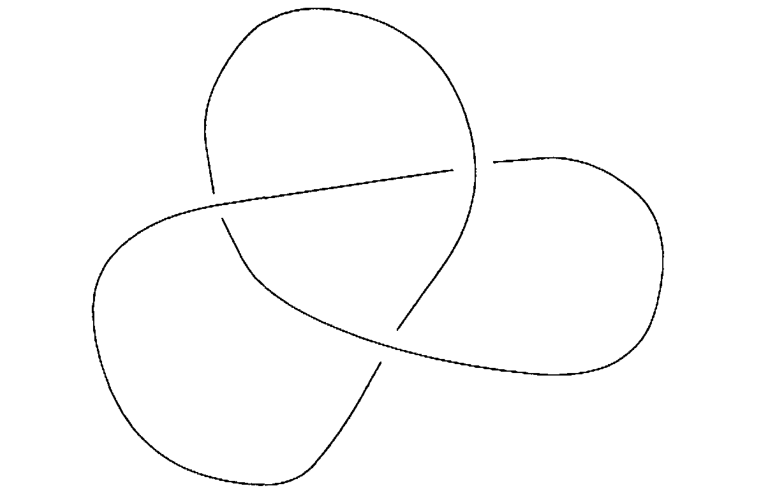
\includegraphics[width=0.44\textwidth]{figs/fig_p121_1.png}
  \caption{三维时空中的一条打结的曲线 $C\subset M$：三维空间中 Wilson 线可以打结，这是三维特有的现象。（原文图示，p.121）}
  \label{fig:p121-1}
\end{figure}

打结的 Wilson 线是我们在三维之外所没有的东西！
对给定的 $C$，我们可以考虑相应的 Wilson 线算符
\begin{equation}
  \tag{8.55}
  \label{eq:8-55}
  \left\langle\mathrm{Tr}_R\,\mathrm{Hol}(A,C)\right\rangle
\end{equation}
其中 $R$ 是 $SU(2)$ 的二维表示，$\mathrm{Hol}$ 表示和乐（holonomy）。
在我们的红外描述（用 $\phi$ 表达）中，这个算符翻译成什么？
正如我们在第 3 节末尾所看到的，它翻译成一条处方：「从时空中删去 $C$，并把 $\phi$ 解释为一个平坦圆周丛的截面，该丛的联络在绕 $C$ 一周时有单值性（monodromy）。」
单值性由角 $2\pi\lambda$ 给出，其中 $\lambda$ 是第 3 节讨论中引入的、出现在 Wilson 圈里的 $U(1)$ 荷（模 $1$）。
我们选取的是处于 $SU(2)$ 二维表示中的 Wilson 线；以 $SO(3)$ 的权格为单位，其 $U(1)$ 荷为 $\pm1/2$（这一事实在上面 Remark 中以另一种方式被利用了）。
因此我们的例子有 $\lambda=1/2$。
于是绕该圆周的单值性是 $\phi\to\phi+\pi$；正如我们刚才注意到的，即使加上了瞬子诱导的相互作用，这也是理论的一个对称性。

现在问题是经典的了：我们要找作用量
\begin{equation}
  \tag{8.56}
  \label{eq:8-56}
  \frac{1}{4\pi e^2}\int|d\phi|^2-2e^{-I/e^2}\int d^3x\left(\cos 2\phi-1\right)
\end{equation}
的极小值，其中 $\phi$ 是一个圆周取值函数，并要求它在绕 $C$ 一周时有单值性 $\pi$。
（我们平移了 $\phi$，使极小能量位于 $\phi=0,\pi$ 处；又从作用量中减去一个常数，使真空能量为零。）
于是，特别地，由于单值性的要求，$\phi$ 不能是常数。
事实上，最小作用量的解近似地由一张以 $\partial\Sigma=C$ 为边界的极小面积曲面 $\Sigma$ 给出；$\phi$ 在远离 $\Sigma$ 处为常数，而在穿过 $\Sigma$ 时跳跃 $\pi$。


% [Tutor Note: (8.56) 中 $\cos 2\phi-1$ 的写法与"跳跃 $\pi$"是配套的，容易看漏：$\cos2\phi$ 在 $\phi\to\phi+\pi$ 下不变（$\cos(2\phi+2\pi)=\cos2\phi$），故 $\phi=0$ 与 $\phi=\pi$ 是两个简并的真空，二者之间才可能存在静态的畴壁（domain wall），也才使下面的极小曲面论证成立；若势写成 $\cos\phi-1$，两个真空之间的能量差会使 $\phi$ 无法在无穷远处取常数值，问题将没有静态解。另外，"$\phi$ 在穿过 $\Sigma$ 时跳跃 $\pi$"之所以是一个好的近似，是因为势的系数 $2e^{-I/e^2}$ 在 $e\to0$ 时指数小：除了一层厚度由 $\frac{1}{4\pi e^2}$ 与 $e^{-I/e^2}$ 之比的平方根给出的薄壁之外，$\phi$ 几乎是自由的，于是作用量由 $\frac{1}{4\pi e^2}\int|d\phi|^2$ 主导，正比于 $\Sigma$ 的面积。按一维化归（把 $\phi$ 看作只依赖于穿墙方向的坐标）可估出弦张力 $\sigma\sim\frac{1}{e}e^{-I/2e^2}$，于是 $\langle W(C)\rangle\sim e^{-\sigma\,\mathrm{Area}(\Sigma)}$，即面积律——这就是禁闭。作者说"现在问题是经典的了"，指的正是 $e\to0$ 时这个半经典（薄壁）极限。]

最容易的情形是 $C$ 为平面中的一条大曲线。
考虑 $\mathbb{R}^3$ 中由 $x=0$ 给出的平面，其中 $x$ 是 $\mathbb{R}^3$ 上的一个线性函数。
令 $C$ 为该平面中一条非常大、本质上无限长的曲线。
我们希望 $\phi$ 在从负 $x$ 走向正 $x$ 时跳跃 $\pi$。
在 $C$ 非常大的极限下，若在深处观测 $\phi$……% 原文在此处跨页，句子于 p.122 续完（"interior of $C$, becomes a function of $x$ only"）。

% 原文 pp.122–127（印刷 pp.1240–1245）

% ===== 原文 p.122 =====
% 承接 p.121 末句（"若在深处观测 $\phi$……"）
在 $C$ 内部的深处，$\phi$ 只作为 $x$ 的函数。于是需要极小化的是
\begin{equation}
  \tag{8.57}
  \label{eq:8-57}
  \int dx\left(\left(\frac{d\phi}{dx}\right)^{2}-2e^{-I/e^{2}}\left(\cos 2\phi-1\right)\right),
\end{equation}
边界条件为：当 $x\to-\infty$ 时 $\phi\to0$，当 $x\to+\infty$ 时 $\phi\to\pi$。
这个带边界条件的变分问题有一个解，且该解在 $x$ 的平移下是唯一的；由于存在质量间隙，$\phi$ 以指数快的速度趋近其渐近值。
记这个一维解的作用量为 $S$。

% [Tutor Note: (8.57) 只是示意性的写法，不能与 (8.56) 逐字对照。把 (8.56) 按 $\phi=\phi(x)$ 约化（另两个方向取单位面积），逐项系数应为 $\frac{1}{4\pi e^{2}}\int dx\big[(\phi')^{2}-8\pi e^{2}e^{-I/e^{2}}(\cos2\phi-1)\big]$；而 (8.57) 相当于把整体因子 $4\pi e^{2}$ 吸收掉、势的系数却仍写作 $2e^{-I/e^{2}}$，两者相差一个因子 $4\pi e^{2}$。也就是说，(8.57) 隐含地对 $x$ 作了一次标度变换并对 $S$ 重新定了标。kink 解的形状、其指数衰减率以及面积律的结论都不受影响，但若照 (8.57) 直接计算 $S$，就会得到关于 $e$ 的错误幂次——弦张力 $\sigma\sim\frac{1}{e}e^{-I/2e^{2}}$ 中的 $1/e$ 只能来自被作者略去的那个整体因子 $\frac{1}{4\pi e^{2}}$。另外，「指数快地趋近渐近值」的依据是势在 $\phi=0,\pi$ 附近的曲率 $m^{2}\propto e^{-I/e^{2}}$，即质量间隙；正因 $m$ 指数地小，畴壁（domain wall）才是「薄」的。]

现在考虑一般的情形：若 $D$ 是以 $C$ 为边界的极小面积曲面，$A(D)$ 是它的面积，那么作为相应平坦丛的截面、且使作用量取极小的那个 $\phi$ 具有如下性质：除 $D$ 附近之外，$\phi$ 都非常接近 $0$ 或 $\pi$；穿过 $D$ 时它跳跃 $\pi$；而在 $D$ 附近，它的剖面看起来正像上一段所讨论的理想化一维问题的解。
它的作用量非常接近 $A(D)S$，因此 Wilson 线的期望值近似为 $e^{-A(D)S}$，这就显示出面积律与禁闭。

\subsection{四维中的对偶与 $SL(2,\mathbb{Z})$}
% 原文 §8.5：Duality in four dimensions and $SL(2,\mathbb{Z})$

接下来我们讨论四维中的阿贝尔对偶（abelian duality），并把它应用于四维自由 $U(1)$ 理论的 $SL(2,\mathbb{Z})$ 对称性。
非自由理论的 $SL(2,\mathbb{Z})$ 对称性，我们留到后面某一讲再讨论，因为迄今所知的所有这类例子都涉及超对称。

我们在一个四维流形 $M$ 上取一个 $U(1)$ 丛 $\mathcal{L}$，以及 $\mathcal{L}$ 上的一个联络 $A$，其曲率为 $F=F_A$。
包含拓扑项的规范理论拉氏量（欧氏符号约定，Euclidean signature）为
\begin{equation}
  \tag{8.58}
  \label{eq:8-58}
  \begin{aligned}
  \mathcal{L}(A)&=\frac{1}{4e^{2}}\int d^{4}x\,\sqrt{g}\,F_{mn}F^{mn}+\frac{i\theta}{16\pi^{2}}\int d^{4}x\,\sqrt{g}\,\epsilon_{mnpq}F^{mn}F^{pq}\\
  &=\frac{1}{2e^{2}}\int F_{A}\wedge *F_{A}+\frac{i\theta}{4\pi^{2}}\int F_{A}\wedge F_{A}.
  \end{aligned}
\end{equation}

我们在动能项上采用了标准的归一化，并把拓扑项归一化，使得把 $\theta$ 换为 $\theta+2\pi$ 不改变物理。
（拓扑项的这一性质来自这样一个事实：$c_{1}(\mathcal{L})^{2}=\int(F_{A}/2\pi)\wedge(F_{A}/2\pi)$ 恒为整数。注意，在自旋流形上 $c_{1}(\mathcal{L})^{2}$ 恒为\emph{偶}整数，于是我们又多出一个等价性：把 $\theta$ 换为 $\theta+\pi$ 也不改变物理。）

令 $\tau=\frac{\theta}{\pi}+\frac{2\pi i}{e^{2}}\in\mathfrak{h}$（$\mathfrak{h}$ 为复上半平面）。
正如我们刚才注意到的，$\tau\mapsto\tau+2$ 是这个理论的一个对称性；而在自旋流形上工作时，$\tau\mapsto\tau+1$ 也是对称性。
要把它扩充为一个 $SL(2,\mathbb{Z})$ 作用（在自旋流形的情形），我们还需要一个把 $\tau$ 映为 $-1/\tau$ 的对称性；这将由对偶变换 $F_{A}\leftrightarrow *F_{C}$ 给出（其中 $C$ 是一个新的「对偶」联络）。

这一对偶变换的计算与 §8.2、§8.3 中的计算类似。
我们先定义 $F_{\pm}=\frac12(F_{A}\pm *F_{A})$，并把拉氏量 (8.58) 改写为
\begin{equation}
  \tag{8.59}
  \label{eq:8-59}
  \begin{aligned}
  \mathcal{L}(A)&=\frac{i\bar\tau}{4\pi}\int F_{+}\wedge F_{+}+\frac{i\tau}{4\pi}\int F_{-}\wedge F_{-}\\
  &=\frac{i\bar\tau}{4\pi}\int\|F_{+}\|^{2}-\frac{i\tau}{4\pi}\int\|F_{-}\|^{2}.
  \end{aligned}
\end{equation}

% [Tutor Note: 由 (8.58) 到 (8.59) 这两步值得逐项验算，因为 $\tau$ 定义中 $\frac{2\pi}{e^{2}}$（而不是 $\frac{\pi}{e^{2}}$）最容易记错。由 $F_{\pm}=\frac12(F_{A}\pm *F_{A})$ 及自对偶/反自对偶性 $*F_{\pm}=\pm F_{\pm}$ 得 $F_{A}=F_{+}+F_{-}$、$*F_{A}=F_{+}-F_{-}$，于是 $F_{A}\wedge *F_{A}=\|F_{+}\|^{2}+\|F_{-}\|^{2}$、$F_{A}\wedge F_{A}=\|F_{+}\|^{2}-\|F_{-}\|^{2}$（交叉项 $F_{+}\wedge F_{-}$ 因次数不相容而消失）。代入 (8.58) 得 $\|F_{+}\|^{2}$ 的系数 $\frac{1}{2e^{2}}+\frac{i\theta}{4\pi^{2}}$、$\|F_{-}\|^{2}$ 的系数 $\frac{1}{2e^{2}}-\frac{i\theta}{4\pi^{2}}$；而 $\frac{i\bar\tau}{4\pi}=\frac{i}{4\pi}\big(\frac{\theta}{\pi}-\frac{2\pi i}{e^{2}}\big)=\frac{1}{2e^{2}}+\frac{i\theta}{4\pi^{2}}$、$-\frac{i\tau}{4\pi}=\frac{1}{2e^{2}}-\frac{i\theta}{4\pi^{2}}$，恰好吻合。第二行那个负号来自 $F_{-}\wedge F_{-}=-\|F_{-}\|^{2}$——反自对偶二形式的外积为负，这是欧氏四维中最常被漏掉的一个符号；若把 $F_{-}\wedge F_{-}$ 也当成 $+\|F_{-}\|^{2}$，就会得出 $\tau$ 与 $\bar\tau$ 位置互换的错误结论，进而把下面模形式的权全部算错。]

% ===== 原文 p.123 =====
记 $\mathcal{G}$ 为与 $A$ 相联系的规范群，则这个理论的配分函数可以写成
\begin{equation}
  \tag{8.60}
  \label{eq:8-60}
  Z(\tau)=\frac{1}{\mathrm{vol}(\mathcal{G})}\sum_{\mathcal{L}}\int\mathcal{D}A\,\exp\left(-\frac{i\bar\tau}{4\pi}\int\|F_{+}\|^{2}+\frac{i\tau}{4\pi}\int\|F_{-}\|^{2}\right).
\end{equation}

我们早先的对偶例子都从这样一个标量场 $\phi$ 的理论出发：$\phi$ 只通过其导数 $d\phi$ 进入拉氏量，因而理论具有 $\phi\mapsto\phi+c$（$c$ 为常数）的对称性；对偶变换的第一步是把这一对称性规范化（gauge），同时引入一个适当的 Lagrange 乘子场。

而现在的理论本身已经是一个规范理论：它是联络 $A$ 的理论，$A$ 只通过其曲率 $F_{A}$ 进入拉氏量，于是理论具有 $A\mapsto A+B$ 的对称性（$B$ 为平坦联络）。
我们要做的，就是「把这一对称性规范化」的类比：允许 $B$ 是任意丛上的任意联络，并引入一种「奇异规范场」（exotic gauge field）$G$——它是一个 2-形式场——把对称性扩充为
\begin{equation}
  \tag{8.61}
  \label{eq:8-61}
  \begin{aligned}
  A&\to A+B\\
  G&\to G+F_{B}.
  \end{aligned}
\end{equation}
于是 $\mathcal{F}:=F_{A}-G$ 扮演「规范不变」量的角色，类似于标量场的协变导数。
需要强调的是：两个 $G$ 场若相差 $G\to G+F_{B}$（$F_{B}$ 为任意线丛上任意联络的曲率），就认为它们是规范等价的。
在我们的分析中，为简单起见，我们假定 $H^{2}(M)$ 没有挠（torsion）。

我们需要拉氏量的一个「规范不变」的扩充。我们或许可以尝试
\begin{equation}
  \tag{8.62}
  \label{eq:8-62}
  \mathcal{L}(A,G)=\frac{i\bar\tau}{4\pi}\int\|\mathcal{F}_{+}\|^{2}-\frac{i\tau}{4\pi}\int\|\mathcal{F}_{-}\|^{2},
\end{equation}
但这太简单了（因为，举例来说，其经典方程给出 $\mathcal{F}=0$）。
为改进这一点，我们在一个新的线丛 $\mathcal{N}$ 上引入一个新的联络 $C$，其曲率为 $F_{C}$，并考虑拉氏量
\begin{equation}
  \tag{8.63}
  \label{eq:8-63}
  \mathcal{L}(A,G,C)=\frac{i\bar\tau}{4\pi}\int\|\mathcal{F}_{+}\|^{2}-\frac{i\tau}{4\pi}\int\|\mathcal{F}_{-}\|^{2}-\frac{i}{2\pi}\int F_{C}\wedge G.
\end{equation}

这个新理论的配分函数可以表示为一个路径积分，其中包含与丛 $\mathcal{L}$ 和 $\mathcal{N}$ 的一切可能选取相对应的各个扇区：
\begin{equation}
  \tag{8.64}
  \label{eq:8-64}
  \begin{aligned}
  &\frac{1}{\mathrm{vol}(\widetilde{\mathcal{G}})}\,\frac{1}{\mathrm{vol}(\mathcal{G})}\,\frac{1}{\mathrm{vol}(\mathcal{G}_{C})}\sum_{\mathcal{L},\mathcal{N}}\int\mathcal{D}A\,\mathcal{D}G\,\mathcal{D}C\\
  &\qquad\times\exp\left(-\frac{i\bar\tau}{4\pi}\int\|\mathcal{F}_{+}\|^{2}+\frac{i\tau}{4\pi}\int\|\mathcal{F}_{-}\|^{2}+\frac{i}{2\pi}\int F_{C}\wedge G\right),
  \end{aligned}
\end{equation}
其中 $\mathcal{G}$ 与 $\mathcal{G}_{C}$ 分别表示与 $A$ 和 $C$ 相联系的规范群，而 $\widetilde{\mathcal{G}}$ 表示「奇异」规范群。

为看出这个新理论与原理论等价，我们先在 (8.64) 中作 $C$ 积分：把 $C$ 写成 $C=C_{0}+C'$，其中 $C_{0}$ 是线丛 $\mathcal{N}$ 上取定的一个联络。于是对 $C'$ 的积分是
\begin{equation}
  \tag{8.65}
  \label{eq:8-65}
  \frac{1}{\mathrm{vol}\,\mathcal{G}_{C}}\int\mathcal{D}C'\,e^{\frac{i}{2\pi}\int C'\wedge dG}=\delta(dG).
\end{equation}

% [Tutor Note: (8.65) 之所以只剩 $\delta(dG)$，关键在于 $\int F_{C'}\wedge G=\int C'\wedge dG$（分部积分，$dG$ 为闭形式时边界项消失），因此这一积分与 $\mathcal{N}$ 的选取、与 $C_{0}$ 都无关，只剩一个纯粹约束 $dG=0$；也正因如此，后面 (8.66) 才能把它与对 $\mathcal{N}$ 的求和分开处理。另一个易错点是：$G$ 是 2-形式，$dG$ 是 3-形式，而 $M$ 是四维的，故 $\delta(dG)$ 是 3-形式空间上的泛函 delta 函数，其「体积」归一化正是 (8.64) 里 $\frac{1}{\mathrm{vol}(\widetilde{\mathcal{G}})}$ 这个因子的来源。若把 $G$ 误当作 1-形式（像通常的 $U(1)$ 对偶那样），就会把 (8.63) 的 $F_{C}\wedge G$ 误写成 $F_{C}\wedge *G$，整个推导随之垮掉。]

% ===== 原文 p.124 =====
于是，当我们对 $\mathcal{N}$ 求和时，得到
\begin{equation}
  \tag{8.66}
  \label{eq:8-66}
  \frac{1}{\mathrm{vol}\,\mathcal{G}_{C}}\sum_{\mathcal{N}}\int\mathcal{D}C\,e^{-\frac{i}{2\pi}\int F_{C}\wedge G}=\sum_{x\in H^{2}(M)}e^{i(x,G)}\,\delta(dG)=\delta\left(\left[\frac{G}{2\pi}\right]\in\mathbb{Z}\right)\delta(dG).
\end{equation}

$dG=0$ 以及 $[G/2\pi]$ 是整上同调类这两个条件，恰恰意味着 $G$ 具有 $F_{B}$ 的形式（$F_{B}$ 是某个线丛上某个联络的曲率），因而意味着 $G$ 可以被规范到零。
做完这一步之后，就可推出配分函数 (8.64) 与 $Z(\tau)$ 一致，于是我们回到了原来的理论。

换一种做法：我们也可以利用「奇异」规范不变性把 $A$ 规范到 $0$，从而计算配分函数 (8.64)。这样剩下的路径积分是
\begin{equation}
  \tag{8.67}
  \label{eq:8-67}
  \frac{1}{\mathrm{vol}\,\mathcal{G}_{C}}\sum_{\mathcal{N}}\int\mathcal{D}G\int\mathcal{D}C\,\exp\left(-\frac{i\bar\tau}{4\pi}\int\|G_{+}\|^{2}+\frac{i\tau}{4\pi}\int\|G_{-}\|^{2}+\frac{i}{2\pi}\int F_{C}\wedge G\right).
\end{equation}

为计算 $G$ 积分，我们配方，同时记住
\begin{equation}
  \tag{8.68}
  \label{eq:8-68}
  \int F_{C}\wedge G=\int\left(F_{C+}\wedge *G_{+}-F_{C-}\wedge *G_{-}\right).
\end{equation}
事实上，若定义 $G'=G-\frac{1}{\bar\tau}F_{C+}+\frac{1}{\tau}F_{C-}$，就可以把 eq. (8.67) 中的指数写成
\begin{equation}
  \tag{8.69}
  \label{eq:8-69}
  -\frac{i\bar\tau}{4\pi}\int\|G'_{+}\|^{2}+\frac{i\tau}{4\pi}\int\|G'_{-}\|^{2}+\frac{i}{4\pi\bar\tau}\int\|F_{C+}\|^{2}-\frac{i}{4\pi\tau}\int\|F_{C-}\|^{2}.
\end{equation}

当我们完成 $G'$ 积分时，前两项给出一个高斯积分，它只对整体归一化有贡献；把 $G'$ 积掉之后，剩下的路径积分是
\begin{equation}
  \tag{8.70}
  \label{eq:8-70}
  \frac{1}{\mathrm{vol}\,\mathcal{G}_{C}}\sum_{\mathcal{N}}\int\mathcal{D}C\,\exp\left(\frac{i}{4\pi\bar\tau}\int\|F_{C+}\|^{2}-\frac{i}{4\pi\tau}\int\|F_{C-}\|^{2}\right).
\end{equation}

这与原来的路径积分相同，只是 $\tau$ 被换成了 $-1/\tau$——这正是我们想要证明的。

% [Tutor Note: (8.69) 的配方建议自己动手复算，因为 $G'$ 的平移量中 $\frac{1}{\bar\tau}$ 与 $\frac{1}{\tau}$ 的搭配不对称，极易写反。以 $G_{+}$ 部分为例，指数为 $-\frac{i\bar\tau}{4\pi}\|G_{+}\|^{2}+\frac{i}{2\pi}\langle F_{C+},G_{+}\rangle$，形如 $a\|G\|^{2}+b\langle F,G\rangle=a\big\|G+\frac{b}{2a}F\big\|^{2}-\frac{b^{2}}{4a}\|F\|^{2}$，此处 $a=-\frac{i\bar\tau}{4\pi}$、$b=\frac{i}{2\pi}$，故 $\frac{b}{2a}=-\frac{1}{\bar\tau}$、$-\frac{b^{2}}{4a}=+\frac{i}{4\pi\bar\tau}$；$G_{-}$ 部分同法给出平移 $-\frac{1}{\tau}F_{C-}$ 与残余项 $-\frac{i}{4\pi\tau}$。四个系数与 (8.69) 逐字相符，可见原文此处无误。真正的物理在残余项：$\frac{i}{4\pi\bar\tau}$ 与 $-\frac{i}{4\pi\tau}$ 恰好是把原作用量中 $\|F_{C+}\|^{2}$、$\|F_{C-}\|^{2}$ 的系数 $\frac{i\bar\tau}{4\pi}$、$-\frac{i\tau}{4\pi}$ 里的 $\tau$ 换成 $-1/\tau$（注意 $\overline{-1/\tau}=-1/\bar\tau$）后所得的结果——高斯积分把 $\tau$ 翻转成 $-1/\tau$，这就是 $S$ 对偶的全部机制，而不是某个额外假设。]

正如我们在两维情形所做的那样，也可以分析路径积分归一化的 $\tau$ 依赖性，从而得到更多有趣的结果。
若计算对 $G'$ 的高斯积分，就能窥见用这种方式所得结果之风味的端倪，该积分给出
\begin{equation}
  \tag{8.71}
  \label{eq:8-71}
  \left(\frac{2\pi}{\sqrt{i\bar\tau}}\right)^{n_{2+}}\left(\frac{2\pi}{\sqrt{-i\tau}}\right)^{n_{2-}},
\end{equation}
其中 $n_{2\pm}$ 表示自对偶与反自对偶 2-形式的个数。
当然，这两个数都是无穷大，所以必定存在与其他归一化因子之间的某种相消。
把这一点详细算出来之后，\footnote{见参考文献中所引的我的论文。}所得的结果是
\begin{equation}
  \tag{8.72}
  \label{eq:8-72}
  Z(\tau)=\tau^{-(\chi+\sigma)/4}\,\bar\tau^{-(\chi-\sigma)/4}\,Z(-1/\tau),
\end{equation}
其中 $\chi$ 与 $\sigma$ 分别是 $M$ 的欧拉数与号差。
于是，配分函数 $Z(\tau)$ 实际上是 $SL(2,\mathbb{Z})$（当流形非自旋时，是某个子群）的一个权为 $\left(\frac{\chi+\sigma}{4},\frac{\chi-\sigma}{4}\right)$ 的模形式（modular form）。

% [Tutor Note: (8.71) 的指数 $n_{2\pm}$ 是自对偶/反自对偶调和二形式的个数：对紧流形它们有限，但一般依赖于度规；而 (8.72) 把幂次换成了 $\frac{\chi+\sigma}{4}$ 与 $\frac{\chi-\sigma}{4}$，其间做了一次正规化。按热核/$\zeta$ 函数正规化，行列式比值的有限部分给出 $n_{2+}\to\frac{\chi+\sigma}{2}$、$n_{2-}\to\frac{\chi-\sigma}{2}$（注意 $\frac{\chi+\sigma}{2}=1-b_{1}+b_{2}^{+}$，正是 de Rham 复形在偶形式上的指标），这就是 Atiyah--Singer 指标定理中 Gauss--Bonnet 与号差两个示性类组合的体现。作者在正文只说「必定存在与其他归一化因子之间的相消」，细节见本讲末参考文献中 E. Witten, \emph{On $S$-duality in abelian gauge theory}, Selecta Math. (N.S.) 1 (1995)。提醒：从 (8.71) 直接读出的权是 $(\frac{n_{2+}}{2},\frac{n_{2-}}{2})$，与 (8.72) 的 $(\frac{\chi+\sigma}{4},\frac{\chi-\sigma}{4})$ 并不相同，两者之差正是上述正规化，切不可混用。]

% ===== 原文 p.125 =====
我们也可以像在低维情形中那样，让某些算符插入穿过对偶变换。
原理论中 $F_{\pm}$ 的插入，在扩充理论中可以由插入 $\mathcal{F}_{\pm}=F_{\pm}-G$ 来实现，而在把变量换成 $G'$ 之后，这可以分别写成
\begin{equation}
  \tag{8.73}
  \label{eq:8-73}
  \mathcal{F}_{+}=F_{+}-G'_{+}-\frac{1}{\bar\tau}F_{C+},\qquad\text{或}\qquad \mathcal{F}_{-}=F_{-}-G'_{-}+\frac{1}{\tau}F_{C-},
\end{equation}
于是，当我们把 $A$ 规范到零并积掉 $G'$ 之后，就只剩下正比于 $F_{C\pm}$ 的算符插入，即：
\begin{equation}
  \tag{8.74}
  \label{eq:8-74}
  F_{+}\mapsto\left(-1/\bar\tau\right)F_{C+},\qquad\text{以及}\qquad F_{-}\mapsto\left(1/\tau\right)F_{C-}.
\end{equation}

请注意：由于这些映射带有 $\tau$ 依赖性，一个含有 $F_{+}$ 与 $F_{-}$ 插入的关联函数，其模权将与配分函数的模权不同。

\subsection{Hamilton 形式}
% 原文 §8.6：The Hamiltonian formalism

回到规范群为 $U(1)$ 的情形。让我们在 Hamilton 框架中简要地讨论四维阿贝尔对偶。
取形如 $M_{3}\times\mathbb{R}$ 的四维流形，其中 $\mathbb{R}$ 是类时方向。
注意这是一个自旋流形，所以我们预期有完整的 $SL(2,\mathbb{Z})$ 对称性。
为简单起见，我们假定 $H_{1}(M_{3})$ 中没有挠。
每个类 $x\in H^{2}(M_{3})$ 决定了三维流形 $M_{3}$ 上的一个复线丛 $\mathcal{L}_{x}$（满足 $c_{1}(\mathcal{L}_{x})=x$）。
我们在三维流形 $M_{3}$ 上的理论，其 Hilbert 空间可以写成如下形式
\begin{equation}
  \tag{8.75}
  \label{eq:8-75}
  \mathcal{H}_{\tau}(M_{3})=\bigoplus_{x\in H^{2}(M_{3},\mathbb{Z})}\mathcal{H}_{x},
\end{equation}
其中 $\mathcal{H}_{x}$ 是把 $\mathcal{L}_{x}$ 上的联络量子化所得的 Hilbert 空间。
（在左端，我们显式标出了对耦合常数 $\tau$ 的依赖。）
为构造 $\mathcal{H}_{x}$，把任意联络写成 $A=A_{0}+\beta$ 的形式，其中 $A_{0}$ 是满足某个规范固定条件的调和联络（harmonic connection，即曲率为调和二形式的联络；规范固定的细节无关紧要），而 $\beta$ 是一个 1-形式。
令 $\mathcal{T}_{x}$ 为线丛 $\mathcal{L}_{x}$ 上调和联络的空间模去规范变换。于是量子化给出
\begin{equation}
  \tag{8.76}
  \label{eq:8-76}
  \mathcal{H}_{x}=\mathcal{H}_{\beta}\otimes L^{2}(\mathcal{T}_{x}).
\end{equation}

这里 $\mathcal{H}_{\beta}$ 是把 $\beta$ 的空间量子化所得的 Hilbert 空间，而 $L^{2}(\mathcal{T}_{x})$ 就是 $\mathcal{T}_{x}$ 上的 $L^{2}$ 函数空间。

注意，因子 $\mathcal{H}_{\beta}$ 与 $x$ 无关，因为 1-形式的空间在定义时并未涉及 $x$。
事实上，$\mathcal{H}_{\beta}$ 是 $M_{3}$ 上一个阿贝尔规范理论的 Hilbert 空间，只不过该理论的规范群不是 $U(1)$，而是它的万有覆盖 $\mathbb{R}$。
对偶把 $\mathcal{H}_{\beta}$ 映到自身，同时分别作用在 $\mathcal{H}'=\bigoplus_{x}L^{2}(\mathcal{T}_{x})$ 上。
对偶在 $\mathcal{H}_{\beta}$ 上的作用由 (8.74) 中的算符映射给出。

对偶在 $\mathcal{H}'$ 上的作用可以这样描述。
注意，所有的 $\mathcal{T}_{x}$ 都是环面 $H^{1}(M_{3},\mathbb{R}/\mathbb{Z})$ 作用下的主齐性空间（principal homogeneous space），而该环面参数化了 $M_{3}$ 上的平坦线丛；$H^{1}(M_{3},\mathbb{R}/\mathbb{Z})$ 中一个元素的作用，就是把给定的线丛（带联络）与相应的平坦线丛作张量积。
令 $y$ 表示阿贝尔群 $H^{1}(M_{3},\mathbb{R}/\mathbb{Z})$ 的一个特征标（character）。存在一个分解
% 原文在此处跨页：句子于 p.126 续完（"decomposition $L^2(\mathcal T_x)=\bigoplus_y\mathcal T_{x,y}$"）。

% [Tutor Note: 这里 $\mathcal{T}_{x}$ 的几何值得写清楚，否则 (8.76)、(8.77) 的分解会显得神秘。两个调和联络之差是闭 1-形式模恰当形式，即 $H^{1}(M_{3},\mathbb{R})$；固定 $c_{1}=x$ 只固定了「拓扑」部分，故 $\mathcal{T}_{x}$ 是一个维数为 $b_{1}$ 的环面，而且是 $H^{1}(M_{3},\mathbb{R}/\mathbb{Z})$ 的主齐性空间（torsor）而非线性空间——(8.75) 左端的 $\tau$ 依赖恰好体现在「哪一个 torsor」上：不同的平坦丛扭转不改变 $L^{2}(\mathcal{T}_x)$ 的 Hilbert 空间结构，只改变其上的平坦联络，这正是 (8.80) 中出现平坦线丛 $\mathscr L_{\theta}$ 的由来。另注意 $\mathcal{H}_{\beta}$ 对应「规范群为 $\mathbb{R}$」而非 $U(1)$：因为 $\beta$ 描述的是 $A$ 偏离调和代表的部分，其「大规范变换」不受整性约束，故其量子化给出的是 $\mathbb{R}$ 规范理论的 Hilbert 空间；这也解释了为什么对偶只作用在 $\mathcal{H}'$ 上（见 (8.74)：$F_\pm$ 的插入只涉及 $F_C$，不涉及 $\beta$）。]

% ===== 原文 p.126 =====
$L^{2}(\mathcal{T}_{x})=\bigoplus_{y}\mathcal{T}_{x,y}$，其中 $\mathcal{T}_{x,y}$ 是 $L^{2}(\mathcal{T}_{x})$ 中按特征标 $y$ 变换的子空间。
每个 $\mathcal{T}_{x,y}$ 都是一维的。因此
\begin{equation}
  \tag{8.77}
  \label{eq:8-77}
  \mathcal{H}'=\bigoplus_{x,y}\mathcal{T}_{x,y}.
\end{equation}

注意，由 Poincaré 对偶与 Pontryagin 对偶，$H^{1}(M_{3},\mathbb{R}/\mathbb{Z})$ 的特征标群是 $H^{2}(M_{3},\mathbb{Z})$。
于是 $x$ 与 $y$ 取值于同一个空间。因此可以交换它们，而这正是 $\tau\to-1/\tau$ 变换所做的（更确切地说，它按 $(x,y)\to(-y,x)$ 作用）。
因此，对偶把一个经典的概念——按 $x$ 所作的分解——与一个量子的概念——按 $y$ 所作的分解——交换了。
关于对偶如何作用的这一断言，将在下面引入算符 $Q_{e}$ 与 $Q_{m}$ 的地方得到验证。

% [Tutor Note: 「由 Poincaré 与 Pontryagin 对偶，$H^{1}(M_{3},\mathbb{R}/\mathbb{Z})$ 的特征标群是 $H^{2}(M_{3},\mathbb{Z})$」这一步，用的正是 p.125 开头「假定 $H_{1}(M_{3})$ 无挠」这一前提，值得补全：$H^{1}(M,\mathbb{R}/\mathbb{Z})=\operatorname{Hom}(H_{1}(M,\mathbb{Z}),\mathbb{R}/\mathbb{Z})$ 的 Pontryagin 对偶是 $H_{1}(M,\mathbb{Z})$ 的\emph{自由部分}，再由 Poincaré 对偶 $H_{1}(M,\mathbb{Z})\cong H^{2}(M,\mathbb{Z})$（配合万有系数定理：$H^{2}$ 的挠部分恰等于 $H_{1}$ 的挠部分）才等于 $H^{2}(M,\mathbb{Z})$。若存在挠，$x$ 与 $y$ 就不再取值于同一集合，$(x,y)\to(-y,x)$ 的写法须改为对 $\operatorname{Hom}$ 的表述，$\mathcal{H}'=\bigoplus_{x,y}\mathcal{T}_{x,y}$ 也不再是同一个环面上的 Fourier 分解。这也说明作者为何在 p.125 一开始就把「无挠」作为简化假设单独提出。]

在量子化时——先暂时略去 $\theta$——人们把四维曲率写成 $F_{A}'+e^{2}\pi_{A}dt$，其中 $F_{A}'$ 是 $M_{3}$ 上的一个二形式，而 $\pi_{A}$——$M_{3}$ 上的一个一形式——是联络 $A$ 的共轭动量。Hamilton 量成为
\begin{equation}
  \tag{8.78}
  \label{eq:8-78}
  H=\int d^{3}x\left(\frac{1}{2e^{2}}F_{A_{0}}^{2}+\frac{e^{2}}{2}\nabla_{A_{0}}^{2}\right)+H(\beta).
\end{equation}

这里 $H(\beta)$ 是 Hamilton 量中作用在 $\mathcal{H}_{\beta}$ 上的那一部分。其余各项作用在 $\mathcal{H}'$ 上。
第一项是调和联络 $A_{0}$ 的磁能；它来自拉氏量中关于 $F_{A}'$ 二次的部分，是 $\int_{M_{3}}x\wedge *x$ 的一个倍数。
第二项来自拉氏量中关于 $\pi_{A}$ 二次的部分，是电能，即 $\mathcal{T}_{x}$ 上的 Laplacian $\nabla^{2}$；它是 $\int_{M_{3}}y\wedge *y$ 的一个倍数。

把 $\theta$ 项包括进来会使量子化发生改变。
事实上，正则动量 $\pi_{A}$——出于后面将显出的理由，我们把它写成 $F_{A}^{\vee}=*\pi_{A}$——可以由原来的拉氏量 (8.58) 定出，其结果为
\begin{equation}
  \tag{8.79}
  \label{eq:8-79}
  F_{A}^{\vee}=2\pi i\frac{\delta\mathcal{L}}{\delta F_{A}}=\frac{2\pi i}{e^{2}}*F_{A}-\frac{\theta}{\pi}F_{A}.
\end{equation}

在 $\theta\ne0$ 时，正则量子化给出的不是 $\mathcal{H}'=\bigoplus_{x}L^{2}(\mathcal{T}_{x})$，而是
\begin{equation}
  \tag{8.80}
  \label{eq:8-80}
  \mathcal{H}'=\bigoplus_{x}\Gamma_{L^{2}}(\mathcal{T}_{x},\mathscr{L}_{\theta}),
\end{equation}
其中 $\mathscr{L}_{\theta}$ 是 $\mathcal{T}_{x}$ 上某个平坦线丛，而 $\Gamma_{L^{2}}$ 表示 $L^{2}$ 截面的空间。
我把辨认 $\mathscr{L}_{\theta}$ 留作读者的一个练习。\footnote{做这个练习的出发点应当是注意到：在一个把联络在时间方向上平凡化的规范中，拉氏量中的 $\theta$ 项是齐次的、并且对时间导数是线性的；任何这样的项都会在相空间上引出一个带联络的线丛。在目前的情形，$\theta$ 项是一个拓扑不变量，从而是经典位形空间上的一个局部常值函数；这就导致线丛 $\mathscr{L}_{\theta}$ 是平坦的。}
当然，$\theta=0$ 时的 $\mathscr{L}_{\theta}$ 就是具有平凡平坦联络的平坦丛；而 $\mathscr{L}_{\theta}$ 只依赖于 $\theta$ 模 $\pi$——我们在自旋流形上，所以 $\theta\to\theta+\pi$ 是一个对称性。

把 $F_{A}^{\vee}$ 的公式用 $\tau$ 改写，我们就能确定这个算符在 $\tau\to-1/\tau$ 下如何变换。
事实上，在算符映射 (8.74) 之下，人们得到
\begin{equation}
  \tag{8.81}
  \label{eq:8-81}
  F_{A}^{\vee}=-\bar\tau F_{+}+\tau F_{-}\mapsto F_{C+}+F_{C-}=F_{C}.
\end{equation}

我们还需要这个计算的「对偶」版本：
\begin{equation}
  \tag{8.82}
  \label{eq:8-82}
  F_{A}=F_{+}+F_{-}\mapsto\overline{\left(-1/\tau\right)}F_{C+}-\left(-1/\tau\right)F_{C-}=-F_{C}^{\vee}.
\end{equation}

% [Tutor Note: (8.79) 与 (8.81) 不可能同时成立，这是本页最需要提防的符号陷阱。把 $\tau=\frac{\theta}{\pi}+\frac{2\pi i}{e^{2}}$、$F_{\pm}=\frac12(F_{A}\pm*F_{A})$ 代入 (8.79) 印出的右端 $\frac{2\pi i}{e^{2}}*F_{A}-\frac{\theta}{\pi}F_{A}$，得到 $-\bar\tau F_{+}-\tau F_{-}$；而 (8.81) 印的是 $-\bar\tau F_{+}+\tau F_{-}$，$F_{-}$ 项差一个符号。三式 (8.81)、(8.82)、(8.83) 构成自洽的一组：把 (8.81) 的形式记作 $F^{\vee}=-\bar\tau F_{+}+\tau F_{-}$，则对 $\tau'=-1/\tau$ 有 $F_{C}^{\vee}=-\bar\tau'F_{C+}+\tau'F_{C-}=\frac{1}{\bar\tau}F_{C+}-\frac{1}{\tau}F_{C-}$，于是 (8.82) 的右端 $\overline{(-1/\tau)}F_{C+}-(-1/\tau)F_{C-}=-\frac{1}{\bar\tau}F_{C+}+\frac{1}{\tau}F_{C-}=-F_{C}^{\vee}$ 恰好成立，(8.83) 的 $Q_{e}\mapsto Q_{m}$、$Q_{m}\mapsto-Q_{e}$ 也随之成立。故 (8.79) 中 $F_{A}$ 与 $*F_{A}$ 两处应互换，即应为 $F_{A}^{\vee}=\frac{2\pi i}{e^{2}}F_{A}-\frac{\theta}{\pi}*F_{A}$；它与 (8.81) 只差这一点。但要注意：p.127 上「$\theta$ 增加 $\pi$ 时 $Q_{e}\mapsto Q_{e}+Q_{m}$」（即 Witten 效应）这句话，用 (8.79) 印出的形式才给出正比于 $Q_{m}$ 的平移，用互换后的形式给出的却是正比于电通量的平移。可见原文此处至少有一处符号笔误；读者务必先固定一套约定（例如以 (8.82)、(8.83) 为准），再自行复核，切勿两式混用。]

% ===== 原文 p.127 =====
在 Hamilton 形式中，对任何 2-循环 $\Sigma\subset M_{3}$，我们都可以在 Hilbert 空间 $\mathcal{H}_{\tau}(M_{3})$ 上定义与之相应的「电」算符与「磁」算符，即令
\begin{equation}
  \tag{8.83}
  \label{eq:8-83}
  \begin{aligned}
  Q_{e}(\Sigma)&=\int_{\Sigma}\frac{F_{A}^{\vee}}{2\pi}=\int_{\Sigma}\frac{F_{C}}{2\pi},\\
  Q_{m}(\Sigma)&=\int_{\Sigma}\frac{F_{A}}{2\pi}=-\int_{\Sigma}\frac{F_{C}^{\vee}}{2\pi}.
  \end{aligned}
\end{equation}
（这些算符只依赖于 $\Sigma$ 在 $H_{2}(M_{3},\mathbb{Z})$ 中的类。）
显然，在 $\tau\to-1/\tau$ 之下，也就是在 $A\to C$ 之下，有 $Q_{e}\to Q_{m}$、$Q_{m}\to-Q_{e}$。
既然 $x$ 与 $y$ 分别是 $Q_{m}$ 与 $Q_{e}$ 的本征值，这就意味着 $\tau\to-1/\tau$ 按 $(x,y)\to(-y,x)$ 作用。
此外，由 $F_{A}^{\vee}$ 的显式公式 (8.79) 可以看出：当 $\theta$ 增加 $\pi$ 时，算符 $Q_{m}$ 不变，而算符 $Q_{e}$ 变为 $Q_{e}+Q_{m}$。
由于我们在自旋流形上，$\theta\to\theta+\pi$ 是一个对称性；它对应于 $\tau\to\tau+1$，并且不改变 Hilbert 空间。

上一段所作的陈述可以合并为如下一句：$SL(2,\mathbb{Z})$ 通过它在序对 $(x,y)$ 上的自然作用而作用在 $\mathcal{H}'$ 上。

\subsection*{参考文献与交叉引用}
% 原文：References and cross references

本讲的主要参考文献为
\begin{itemize}
  \item T. Buscher, \emph{Path integral derivation of quantum duality in nonlinear sigma models}, Phys. Lett. B \textbf{201} (1988), 466--472.
  \item E. Witten, \emph{On $S$-duality in abelian gauge theory}, Selecta Math. (N.S.) \textbf{1} (1995), 383--410.
  \item A. M. Polyakov, \emph{Gauge Fields and Strings}, Harwood Academic Publishers, 1987（特别是 pp.~62--72）.
  \item S. Coleman, \emph{Aspects of Symmetry}, Cambridge University Press, 1985（论「Lumps」的那一章）.
\end{itemize}


\clearpage
% 原文 pp.129–136（印刷 pp.1247–1254）
\section{Lecture 9：孤子}

\begin{keytakeaways}
本讲把「孤子」定义为庞加莱不变场论之经典场方程的行波解：空间局域、能量有限，并在给定同伦类中取能量的全局极小。核心数学工具是把孤子与「有限能量经典解空间的连通分支」联系起来：孤子在解空间中的 $P$-轨道 $\mathcal{O}=P/P_s$ 同构于余切丛 $T^*\mathcal{O}^+_m$，其量子化给出 $P$ 的不可约表示 $\mathbf{L}^2(\mathcal{O}^+_m)$，且孤子分支的 Hilbert 空间没有真空、能谱有正的下界。孤子质量随作用量整体常数 $C$ 线性增长（$\sim C$），远重于微扰粒子，故微扰论看不见孤子。在 $1+1$ 维含费米子的模型中，孤子携带费米零模，使最低能态空间成为 $\mathbf{L}^2(\mathcal{O}^+_m)\otimes S$（$n$ 为偶数时）。在 $3+1$ 维 $SO(3)$ 规范理论中孤子即磁单极子，其无穷远处第一 Chern 类 $c_1$ 必为偶数；加入 $\theta$ 角后正则动量被移动，于是 $Q_e=\frac{\theta}{2\pi}Q_m\bmod\mathbb{Z}$，晶格在 $\theta\to\theta+2\pi$ 下的单值变换给出 Witten 效应。
\end{keytakeaways}

% ===== 原文 p.129 =====
\subsection{什么是孤子？}
% 原文 §9.1：What is a soliton?

在经典数学物理中，所谓孤子（soliton）通常指非线性偏微分方程 $u_t=F(u,u_x,\dots)$ 的「行波」（traveling wave）解，即形如 $u(x,t)=f(x-vt)$ 的解。
孤子在可积系统理论中起着非常重要的作用：在该理论中（在某些情形下）任何解都可由以不同速度运动的孤子的叠加来逼近。
因此，可积系统理论有时也被称为孤子理论。

今天我们感兴趣的，则是场论中出现的孤子（作为经典场方程的行波解），并且主要是它们在场的量子化中所扮演的角色。
这与可积系统理论中的观点不同。
特别地，我们并不声称孤子之间存在非线性叠加；我们所考察的模型一般说来也不是精确可积的。

我们将考虑闵可夫斯基空间上庞加莱（Poincaré）不变的场论中的孤子。
对某个具体的场论，我们把孤子理解为场方程的一个行波解（即依赖于 $x-vt$ 的解），它在空间中是局域的，并且能量有限。
由庞加莱不变性，总可以假设 $v=0$，即该解与时间无关。
我们最关心的是这样的孤子：它在相应的同伦类中给出能量的全局极小。

\textbf{注（Remark）.}
把孤子与瞬子（instanton）区分开来十分重要。
瞬子局域于欧氏时空之中（即只存在一个瞬刻），其作用量有限；而孤子局域于（闵可夫斯基时空的）空间之中，永远存在，能量有限。
二者的物理应用完全不同。今天我们关心的是孤子。

% [Tutor Note: 「在相应同伦类中给出能量全局极小」这一限制并非多余。以 $1+1$ 维 $\phi^4$ 模型为例，分支 $X_{+-}$ 上能量泛函的临界点只有 kink（连同其平移与 boost），它自动是极小；但在分量更多的模型（$CP^{n}$ 模型、非阿贝尔规范理论）中，同一同伦类内可以有多个临界点，只有满足一阶 Bogomolny 方程的才是全局极小，其余是鞍点。作者在第 1249 页假设极小值非退化（横截方向二阶导数为正），正是为了保证孤子附近的态可按简谐振子量子化、而不会混入其它临界点的贡献。]

% [Tutor Note: 「由庞加莱不变性总可设 $v=0$」的准确含义是：若 $\phi(x,t)$ 是解，则任一 boost $\Lambda$ 给出新解 $\phi(\Lambda^{-1}(x,t))$，其能量为 $E\to\gamma E$。因此「在质心系中取能量极小」与「在任意惯性系中取能量极小」等价，孤子的静止系总是可以选定的；这也解释了后文 $P$-轨道 $\mathcal{O}=P/P_s$ 为何要以静止解的稳定化子 $P_s$ 作商。]

\subsection{孤子与经典解空间的连通分支}
% 原文 §9.2：Solitons and components of the space of classical solutions

经典地看，孤子的存在与「有限能量的经典解空间具有不同的连通分支」这件事密切相关。
在不包含零能量解的连通分支中，能量的极小值往往在某个孤子上达到。

% ===== 原文 p.130 =====
作为例子，可以回想第 1 讲中讨论过的情形：势为 $U=(\phi^2-a^2)^2$ 的二维标量场论。
此时，有限能量的、与时间无关的经典解空间有 4 个连通分支：$X_{++}$、$X_{-+}$、$X_{+-}$、$X_{--}$，其中
\[
X_{+-}=\{\phi:\ \phi(-\infty)=a,\ \ \phi(\infty)=-a\},
\]
其余符号取法类似。
在其中两个分支 $X_{+-}$ 与 $X_{-+}$ 上，能量严格为正，且其极小值分别在某个孤子解上达到。
这些解分别形如 $\phi=f(x)$ 与 $\phi=-f(x)$，其中 $f(x)$ 是势 $-U$ 所对应的牛顿方程 $f''=U'(f)$ 的、满足边界条件「在 $-\infty$ 处取值 $a$、在 $\infty$ 处取值 $-a$」的解。
证明这样的解存在、且在 $x$ 的平移下唯一，是初等的。

% [Tutor Note: 「$f''=U'(f)$，对应势 $-U$」这一句把两件事说成了一句话，容易读错：能量泛函是 $E=\int dx\,[\tfrac12(f')^2+U(f)]$，若把 $x$ 当作「时间」，则 $f(x)$ 满足粒子在势 $V=-U$ 中的牛顿方程 $f''=-V'(f)=U'(f)$。kink 相当于粒子从 $-U$ 的一个极大点「滚」到另一个极大点、且两端速度为零的轨道，能量守恒给出 $\tfrac12(f')^2=U(f)$，于是 $E=\int dx\,(f')^2$——这正是饱和了的 Bogomolny 界，也解释了为何 kink 是该分支上的全局极小而非鞍点。]

注意，孤子并不在庞加莱群下不变。
但人们常遇到在空间中绕某个「质心」具有旋转对称性的孤子。
在标量场论中，这意味着该孤子的对称群是 $P_s=SO(d-1)\times\mathbb{R}$。
由于庞加莱群是 $P=SO(d-1,1)\ltimes\mathbb{R}^{d-1,1}$，孤子在解空间中的 $P$-轨道 $\mathcal{O}$（即商 $P/P_s$）便是上半个双叶双曲面上的一个 $(d-1)$ 维向量丛。
以下几条容易验证。

% [Tutor Note: 作者称 $P/P_s$ 是「$(d-1)$ 维向量丛」，数一下维数便可确认：$\dim P=\frac{d(d-1)}{2}+d$，$\dim P_s=\frac{(d-1)(d-2)}{2}+1$，故 $\dim(P/P_s)=2(d-1)$，恰为底流形（双曲面，$(d-1)$ 维）的维数加上纤维维数 $(d-1)$；而 $T^*\mathcal{O}^+_m$ 的维数同样是 $2(d-1)$，这正是下面第 3 条中辛微分同胚得以存在的前提。]

\begin{enumerate}
\item 该丛自然同构于双曲面的余切丛。
\item 解空间上的辛结构限制到 $\mathcal{O}$ 上非退化，从而在 $\mathcal{O}$ 上定义了一个辛结构。
\item （辛形式的归一化）设 $m$ 为孤子的质量（即质心系中的能量）。
  则存在一个 $P$-等变的辛微分同胚
  \[
  \mathcal{O}\to T^*\mathcal{O}^+_m,
  \]
  其中 $\mathcal{O}^+_m$ 是 $\mathbb{R}^{d-1,1}$ 中双曲面 $x^2=-m^2$ 的上半部分。
\end{enumerate}

\subsection{孤子与量子化}
% 原文 §9.3：Solitons and quantization

在上述例子这类「经典解空间有若干不相连分支」的情形中（此例中即 $X_{\pm\pm}$），人们预期量子 Hilbert 空间是若干子空间的直和，每个分支对应一个子空间。
若 $X$ 是经典解空间的一个分支，且其中含有庞加莱不变的极小能量解，则可以预期 $X$ 的量子化将给出一个含有庞加莱不变态的 Hilbert 空间。
在上面的例子中，$X_{++}$ 与 $X_{--}$ 含有这样的庞加莱不变解（$\phi=a$ 或 $-a$）。
但 $X_{+-}$ 与 $X_{-+}$ 没有；在这些分支上，极小能量解是孤子或反孤子。
一般地，在不含庞加莱不变的最小能量解的分支中，最小能量解总是某种孤子。
因此我们把这样的分支称为孤子型（solitonic）分支。

设 $X_s$ 是一个孤子型分支。
那么，考虑孤子解的一切庞加莱变换，我们如上得到一个辛嵌入
\[
T^*\mathcal{O}^+_m\to X_s,
\]
其中 $m$ 是孤子解 $s$ 的质量。
我们假定能量在此映射的像上的极小值是非退化的，意思是：不存在能量为 $m$ 的其它解，且能量沿横截于该像的方向的二阶导数为正。

在此情形下，在弱耦合区域我们应当预期：

% ===== 原文 p.131 =====
\begin{enumerate}
\item 量子理论 Hilbert 空间 $\mathcal{H}$ 的分支 $\mathcal{H}_s$ 没有真空（因为经典上没有庞加莱不变解）。
\item $\mathcal{H}_s$ 上的哈密顿量 $H$ 满足不等式 $H\ge m'$，其中 $m'$ 是某个正的质量参数，且当耦合趋于零时 $m'\to m$（一般说来，应当预期 $m$ 会得到量子修正）。
  若理论有质量间隙，则应预期：当耦合趋于零时质量收敛到 $m$ 的那些态，构成 $T^*\mathcal{O}^+_m$ 的一个量子化，即 $P$ 的形如 $\mathbf{L}^2(\mathcal{O}^+_m)$ 的不可约表示。
  由于二阶导数为正，还应预期 $m$ 附近的谱是离散的。
\end{enumerate}

注意，若理论的（作用量或）能量泛函乘以一个常数 $C$，则孤子的质量也乘以 $C$，而通常粒子的质量不变。
回想一下，在这种情形下耦合常数按 $C^{-1}$ 标度。
这意味着，在半经典（弱耦合）近似（$C\to\infty$）下，孤子比通常粒子重得多。
因此，孤子不可能在微扰论中被看到：含孤子的中间态对关联函数的贡献在弱耦合极限下是指数级小的。
这正是我们此前能够在完全不讨论孤子的情况下走到这一步的原因！

% [Tutor Note: 「$C\to\infty$ 即弱耦合」的依据是把 $C$ 吸收进 $\hbar$：路径积分为 $\int\mathcal{D}\phi\,e^{\frac{i}{\hbar}C S_0}$，故展开参数是 $\hbar/C$，令 $\hbar=1$ 后即为 $1/C$，与作者所说的「耦合按 $C^{-1}$ 标度」一致。孤子质量 $M=C\,M_{\text{cl}}$ 随 $C$ 线性增长，微扰粒子质量则与 $C$ 无关；于是孤子中间态给出 $\sim e^{-M\Delta t}=e^{-C M_{\text{cl}}\Delta t}$ 的压低。注意这里说的是「指数小」而非「幂次小」，故任何有限阶微扰展开都看不见孤子。]

% [Tutor Note: 第 2 条中 $H\ge m'$ 与「无真空」是同一拓扑事实的两种表述：孤子分支的经典解在空间无穷远处取非平凡边界条件，任何有限能量的场组态都无法连续变形到 $\phi\equiv a$，故量子化后该分支的 Hilbert 空间里不存在 $P$-不变的基态。$m'$ 与 $m$ 的差别正是 $1/C$ 阶的量子修正（零点能、Casimir 型贡献），作者用 $m'\to m$ 把它一笔带过。]

\subsection{含费米子的理论中的孤子}
% 原文 §9.4：Solitons in theories with fermions

在含费米子的理论中，孤子在 $P$ 下的轨道往往不是解空间相应连通分支中最低能态的全体。
例如，若模型是超对称的，则先验地显然该轨道不是最低能量解的全体：最低能态的空间是超庞加莱群的轨道，而不只是庞加莱群的轨道。
即便没有超对称，费米子也常常在孤子的量子化中起重要作用。

让我们看一个这样的例子。考虑二维的、含一个标量与一对费米子的理论：
\begin{equation}
  \tag{9.1}
  \label{eq:9-1}
  \mathcal{L}=\frac{1}{2\lambda}\int d^2x\bigl(|\partial\phi|^2+(\phi^2-a^2)^2\bigr)
  +i\int d^2x\bigl(\psi_+\partial_-\psi_++\psi_-\partial_+\psi_--g\phi\psi_+\psi_-\bigr).
\end{equation}

\textbf{注 1（Remark 1）.}
对 $g$ 的某个适当取值，此模型是超对称的；但我们并不限于这个取值。

\textbf{注 2（Remark 2）.}
此模型具有手征对称性 $\phi\to-\phi$、$\psi_\pm\to\pm\psi_\pm$，它禁止费米子的质量项 $m\psi_+\psi_-$。

考虑理论玻色部分的孤子 $\phi(x,t)=f(x)$（在 $\phi=a$ 与 $\phi=-a$ 之间插值）。
此解的费米子推广是有限能量的函数 $\psi(x)=\begin{pmatrix}\psi_+(x)\\ \psi_-(x)\end{pmatrix}$，满足 Euler–Lagrange 方程
\begin{equation}
  \tag{9.2}
  \label{eq:9-2}
  \left[\partial_x\psi+\begin{pmatrix}0&-gf(x)\\-gf(x)&0\end{pmatrix}\right]\psi=0.
\end{equation}
于是
\begin{equation}
  \tag{9.3}
  \label{eq:9-3}
  \psi=\begin{pmatrix}\varepsilon\\ \varepsilon\end{pmatrix}
  \exp\Bigl(g\int_0^x f(y)\,dy\Bigr)
  +\begin{pmatrix}\varepsilon'\\ -\varepsilon'\end{pmatrix}
  \exp\Bigl(-g\int_0^x f(y)\,dy\Bigr),
\end{equation}

% [Tutor Note: (9.2) 的记号略有滥用：方括号内是作用在二分量 $\psi$ 上的算符 $\partial_x+\begin{pmatrix}0&-gf\\-gf&0\end{pmatrix}$，而 $\psi$ 同时出现在方括号内外；按字面读作 $[\partial_x+M(x)]\psi=0$ 即可。(9.3) 就是该常微分方程的通解：矩阵 $M$ 的两个本征向量 $(1,1)$ 与 $(1,-1)$ 分别对应本征值 $\mp gf$，故指数分别是 $\pm g\int_0^x f$。]

% ===== 原文 p.132 =====
其中 $\varepsilon,\varepsilon'$ 是奇变量。
容易看出，对孤子（$f>0$ 当 $x\to\infty$，$f<0$ 当 $x\to-\infty$）而言，恰好 $\varepsilon=0$ 的那些解属于 $\mathbf{L}^2$，于是有限能量解的空间是一维的。
对反孤子同样，恰好 $\varepsilon'=0$ 的那些解属于 $\mathbf{L}^2$。
在真空分支中（$f$ 在 $x\to\pm\infty$ 时同号），没有 $\mathbf{L}^2$ 解。

% [Tutor Note: 判断哪个指数被 $\mathbf{L}^2$ 排除，只看 $x\to\pm\infty$ 的渐近行为即可：$f(\pm\infty)=\pm a$，故 $\exp(\pm g\int_0^x f)$ 分别按 $e^{\pm gax}$ 增长或衰减。第一项在 $x\to+\infty$ 发散，必须取 $\varepsilon=0$；第二项在两端都衰减，于是只剩一个（由奇参数 $\varepsilon'$ 标记的）归一化解——这就是「恰有一个费米零模」。零模的存在依赖于 $f$ 的拓扑（kink）；真空分支中两端同号，两个指数在某一端都发散，故无 $\mathbf{L}^2$ 解。]

于是，考察孤子分支，我们便得到费米子的唯一一个零能 $\mathbf{L}^2$ 解。
我们可以把模型稍作推广，使之不含单独一对费米场 $\psi_+,\psi_-$，而含 $n$ 对 $\psi_{\pm i}$，$i=1,\dots,n$，每一对都通过与方程 (9.1) 中相同的耦合与 $\phi$ 相互作用。
于是拉氏量的费米子部分为
\[
\sum_{i=1}^{n}i\int d^2x\bigl(\psi_{+i}\partial_-\psi_{+i}
+\psi_{-i}\partial_+\psi_{-i}-g\phi\psi_{+i}\psi_{-i}\bigr).
\]
费米子上按自然方式作用着 $SO(n)$ 对称性。
此时有 $n$ 个费米子解，故最低能量解的庞加莱轨道不是 $T^*\mathcal{O}^+_m$，而是超流形 $T^*\mathcal{O}^+_m\times\mathbb{R}^{0|n}$。

因此，若 $n$ 为偶数，量子理论中 Hilbert 空间相应分支里的最低能态空间是 $\mathbf{L}^2(\mathcal{O}^+_m)\otimes S$，其中 $S=S_++S_-$ 是 $Spin(n)$ 的自旋表示。
$n$ 为奇数时描述略为微妙，今天我们不去分析这种情形。（关于其要点的说明，见第 12 讲第 3 部分的末尾。）

% [Tutor Note: $n$ 为偶数时 $Spin(n)$ 有两个不等价的半自旋表示 $S_\pm$，费米数的 $\mathbb{Z}_2$ 分次与 $S=S_++S_-$ 的分解相容，故基态空间 $\mathbf{L}^2(\mathcal{O}^+_m)\otimes S$ 有良好定义。$n$ 为奇数时 $Spin(n)$ 只有一个自旋表示，$Cl(n)$ 的不可约模不能自然地按费米数分半，孤子基态的费米奇偶性因而没有先验定义——这正是作者称「描述更微妙」并指向第 12 讲第 3 部分的原因。]

\subsection{$2+1$ 维与 $3+1$ 维中的孤子}
% 原文 §9.5：Solitons in 2+1 and 3+1 dimensions

尽管瞬子与孤子有区别，二者之间仍有联系。
即：$d-1$ 维欧氏场论中的一个瞬子，往往给出同一理论 $d$ 维闵可夫斯基版本中的一个孤子。
例如，考虑带复标量的 $2+1$ 维 $U(1)$ 规范理论：
\begin{equation}
  \tag{9.4}
  \label{eq:9-4}
  \mathcal{L}=\int d^3x\left(\frac{F_A^2}{4e^2}
  +\frac{1}{\lambda}\bigl(|d_A\phi|^2+(|\phi|^2-a^2)^2\bigr)\right).
\end{equation}
在第 7 讲我们看到，此理论的二维版本有 Chern 类为 $1$ 和 $-1$ 的瞬子。
在 $2+1$ 维理论中，这些瞬子变成孤子，并如上所述支配 Hilbert 空间相应分支中的最低能模式。

现在考虑 $3+1$ 维的非阿贝尔规范理论。
即考虑带三维表示中玻色子的 $SO(3)$ 规范理论，其拉氏量为
\begin{equation}
  \tag{9.5}
  \label{eq:9-5}
  \mathcal{L}=\int d^4x\left(\frac{\operatorname{Tr}F_A^2}{4e^2}
  +\frac{1}{2\lambda}\bigl(|d_A\phi|^2+(|\phi|^2-a^2)^2\bigr)\right).
\end{equation}
% [Tutor Note: 注意 (9.4) 与 (9.5) 中标量势项的系数不同：$1/\lambda$ 对 $1/(2\lambda)$（规范项则都是 $F_A^2/4e^2$）。这不是笔误：$d=3$ 时 $[\phi]=1/2$、$[\lambda]=-1$，$d=4$ 时 $[\phi]=1$、$[\lambda]=0$，两处的 $\lambda$ 是量纲不同的参数，相对因子 $2$ 可完全吸收进 $\lambda$ 的定义。但若要把两式放在一起比较（例如核对单极子质量公式 $M\sim4\pi a/e$ 的系数），就必须先统一约定，否则会凭空差一个因子 $2$。]
我们可以把 $A$ 看作秩三实向量丛 $E$ 上的联络，把 $\phi$ 看作 $E$ 的截面。
我们在第 8 讲中考虑过此理论的三维版本。
为方便起见，我们把时空 $\mathbb{R}^3$ 与规范群的李代数、以及 $\phi$ 的取值空间等同起来（李代数中的括号就是叉积）。
这使我们能把标量场 $\phi$ 与无穷小规范变换写成 $\mathbb{R}^3$ 上的向量场。

% ===== 原文 p.133 =====
我们发现，在三维情形此理论有一个瞬子，其中 $\phi$ 形如
\[
\vec\phi=\frac{\vec x}{r}f(r),\qquad r=|\vec x|
\]
（如我们已经说明的，我们把时空与 $\phi$ 的取值空间等同起来，故 $\vec\phi$ 与位置 $\vec x$ 都是三维向量）。
在 4 维中，这个瞬子将变成一个孤子。
这类孤子称为磁单极子（magnetic monopole），因为它们相对于低能未破缺的 $U(1)$ 规范理论确实带有经典意义上的磁荷。

为更好地理解这一点，回想：任何有限能量的场组态 $(A,\phi)$ 都定义一个整值拓扑不变量——「无穷远处的第一 Chern 类 $c_1$」。
的确，为使能量有限，必须在无穷远处有 $|\phi|=a$，于是 $\phi$ 定义了从 $\mathbb{R}^3$ 中无穷远处的球面到半径为 $a$ 的球面的一个映射，而 $c_1$ 是这个映射的度的两倍。

$c_1$ 的另一个定义（它或许更能说明该不变量为何叫 $c_1$、以及在何种意义上 $c_1$ 是上述映射的度的两倍）如下：截面 $\phi$ 在无穷远处把我们的三维向量丛 $E$ 分裂为直和 $\mathbb{R}\phi\oplus\phi^{\perp}$，即一个一维与一个二维向量丛。
（这里 $\mathbb{R}\phi$ 是 $E$ 中由与 $\phi$ 成比例的向量构成的子丛，$\phi^{\perp}$ 是正交补。）
于是 $\phi$ 在无穷远处把结构群约化为 $SO(2)=U(1)$。
数 $c_1$ 就是 $U(1)$ 丛 $\phi^{\perp}$ 限制到 $\mathbb{R}^3$ 中无穷远 2-球面上所得的第一 Chern 类。
例如，上面讨论的孤子组态有 $c_1=2$，因为此时 $SO(2)$ 丛正是无穷远处球面的切丛，而球面的 Euler 示性数为 $2$。
在本模型中，在无穷远处测得的 $c_1$ 总是偶数，故 $2$ 是最小的可能正值。
其为偶数的理由是：由于 $\mathbb{R}^3$ 可缩，$E$ 的第二 Stiefel–Whitney 类为零，于是我们可以过渡到 $SO(3)$ 的双覆盖 $SU(2)$，并考虑与 $E$ 相伴的秩二复向量丛 $W$。
Higgs 场 $\phi$ 在无穷远处把 $W$ 分裂为 $\mathcal{T}\oplus\mathcal{T}^{-1}$，其中 $\mathcal{T}$ 是某个线丛；$\mathcal{T}$ 的第一 Chern 类等于用 $SO(3)$ 丛定义的 $c_1$ 的一半，故后者总是偶数。
当然，无穷远处的第一 Chern 类在第 8 讲中也以大致相同的方式引入过。

% [Tutor Note: 「$c_1$ 是映射 $\phi/|\phi|:S^2_\infty\to S^2_a$ 的度的两倍」与「上述孤子组态有 $c_1=2$」必须一致地理解，否则容易以为差了因子 2：标准 't Hooft–Polyakov 单极子取 $\phi^a=\hat x^af(r)$，$\phi/|\phi|$ 是恒等映射（度 $1$），而 $\phi^{\perp}$ 在 $S^2_\infty$ 上的限制恰为 $TS^2$，$\int_{S^2}c_1(TS^2)=\chi(S^2)=2$，故 $c_1=2$、磁荷 $c_1/2=1$。因子 $2$ 正是「$SO(3)$ 丛的 $c_1$ 等于 $SU(2)$ 提升下线丛 $c_1$ 的两倍」这一事实的另一面，也是本模型中 $c_1$ 必为偶数的根源。]

% [Tutor Note: 「$\mathbb{R}^3$ 可缩故 $w_2(E)=0$，于是可过渡到双覆盖 $SU(2)$」这一步省略了：$w_2\in H^2(\mathbb{R}^3;\mathbb{Z}_2)=0$ 是 $SO(3)$ 丛提升为 $SU(2)$ 丛的障碍类，障碍为零故提升存在；而 $SU(2)$ 的秩二复表示 $W$ 上，$\phi$ 在无穷远处给出 $W=\mathcal{T}\oplus\mathcal{T}^{-1}$ 的分解，$\mathcal{T}$ 与 $\mathcal{T}^{-1}$ 的 $c_1$ 互为相反数，故 $c_1(W)=0$，这与 $W$ 来自 $SU(2)$ 丛相容。]

此理论的孤子解被称为磁单极子，理由如下。
在无穷远处（或在真空中），规范对称性通过我们本学期第 2 讲所研究的 Higgs 机制自发破缺，从 $SO(3)$ 破缺到 $SO(2)=U(1)$。
于是低能理论看起来像一个 $U(1)$ 阿贝尔规范理论。
无穷远处的第一 Chern 类度量的是「磁场」（低能 $U(1)$ 理论的曲率 $F/2\pi$）在无穷远处球面上的积分；在经典物理中，这个积分被称为总磁荷。（我们将在下文 (9.9) 式给出磁荷的形式定义。）
人们通常把 $c_1/2$ 称为该解的磁荷。

现在讨论这样一个事实对孤子的一项推论：无穷远处规范群的未破缺子群是 $U(1)$。
这个 $U(1)$ 是真空、或无穷远处场的对称性；但它并不保持完整的孤子（磁单极子）解不变。
作用在某个特定解上，它会产生一个新的解。
为理解这个作用，让我们考察上面讨论过的、$c_1=2$ 的孤子 $(A,\phi)$。
我们把 $U(1)$ 群的无穷小生成元表示为球对称的规范对称性：$\varepsilon=\frac{\vec x}{r}g(r)$，其中 $g$ 是某个函数。
若函数 $g(r)$ 满足 $r\to0$ 时 $g(r)\sim c_0r$、以及 $g(+\infty)=c$，则此式定义了规范变换李代数中一个光滑元素，它在无穷远处是「常数」的（相对于由标量场 $\phi$ 所定义的结构群约化）。

% ===== 原文 p.134 =====
若愿意，我们可以取 $\varepsilon=\phi/a$，这是一个完全自然、且满足全部条件的选择。
于是 $\varepsilon$ 的作用为
\begin{equation}
  \tag{9.6}
  \label{eq:9-6}
  A\to A-d_A\varepsilon,\qquad \phi\to\phi.
\end{equation}
显然 $d_A\varepsilon$ 不可能恒为零，因为孤子的联络 $A$ 并不具有整体约化到 $U(1)$ 的结构群；因此不存在协变常数的 $\varepsilon$。
所以，位于无穷远处未破缺群中的那些规范变换，其作用是非平凡的。
现在考虑作规范变换 $\exp(c\varepsilon)$。
若 $c\in2\pi\mathbb{Z}$，则该规范变换在无穷远处趋于恒等。
在量子化时，我们把相差一个「在无穷远处趋于恒等」的规范变换的两个场视为同一，故对这样的 $c$，应认为 $\exp(c\varepsilon)$ 平凡地作用。
模去在无穷远处等于 $1$ 的规范变换，那些保持无穷远处场不变的规范变换生成未破缺的 $U(1)$，而这个群自由地作用在孤子解的空间上。

% [Tutor Note: 取 $\varepsilon=\phi/a$ 时，由 $\phi=\frac{\vec x}{r}f(r)$ 得 $g(r)=f(r)/a$；光滑性要求 $r\to0$ 时 $f(r)\sim c_0'r$，故 $g(r)\sim(c_0'/a)r$，又 $f(\infty)=a$ 给出 $g(+\infty)=1$，两条要求恰好满足。这也说明「常数 $c$」的量子化条件为何是 $c\in2\pi\mathbb{Z}$：$\varepsilon=\phi/a$ 在无穷远处取值于单位球面，而 $so(3)$ 中绕单位轴转 $2\pi$ 回到恒等，故 $\exp(c\varepsilon)|_{\infty}=1$ 当且仅当 $c$ 是 $2\pi$ 的整数倍。]

% [Tutor Note: 「依赖时间的孤子空间是 $T^*\mathcal{O}\times T^*S^1$」这一步是作者跳过的：静态孤子的模空间是 $\mathcal{O}\times S^1$（质心位置与 $\alpha$ 角），而场论中任一静态解的速度自由度总由「模空间坐标 + 其共轭动量」参数化，故依赖时间解的模空间是余切丛。平移给出 $T^*\mathbb{R}^3\subset T^*\mathcal{O}$，而 $\alpha=\alpha_0+st$ 给出 $T^*S^1$ 的纤维方向；注意 $s$ 只是 $\alpha$ 的「速度」，与 $\alpha$ 共轭的动量才是后文的电场荷 $Q_e$，二者差一个由辛形式归一化决定的常数。]

同时允许空间平移，上述论证表明：磁荷为 $1$ 的、依赖时间的孤子构成的空间至少是 $\mathbb{R}^3\times S^1$（$\mathbb{R}^3$ 与 $S^1$ 上都没有典则的零点）。
可以证明，事实上它恰好就是如此。
我们把 $S^1$ 因子上的圆坐标记作 $\alpha$。

利用庞加莱群变换，我们可以生成依赖时间、以常速传播的解。
我们也可以作依赖时间的规范变换，这会使 $\alpha$ 坐标依赖时间，即 $\alpha=\alpha_0+st$，$s\in\mathbb{R}$。
结果，依赖时间的孤子构成的空间是乘积 $T^*\mathcal{O}\times T^*S^1$。

\subsection{带 $\theta$ 角的 $3+1$ 维理论}
% 原文 §9.6：The 3+1-dimensional theory with the θ-angle

考虑上一节 $3+1$ 维理论并加入 $\theta$ 角，即在我们（闵可夫斯基）的拉氏量中添上一项
\begin{equation}
  \tag{9.7}
  \label{eq:9-7}
  -\frac{\theta}{16\pi^2}\int\operatorname{Tr}(F\wedge F).
\end{equation}
我们回想，第二 Chern 类 $c_2$ 由积分 $\frac{1}{8\pi^2}\int\operatorname{Tr}(F\wedge F)$ 给出。
因此，经典地看，项 (9.7) 只是数出丛的第二 Chern 类。

现在考虑我们理论中的三个算符：
\begin{enumerate}
\item 未破缺 $U(1)$ 的生成元，我们把它写作 $\frac{\partial}{\partial\alpha}$，其中 $\alpha$ 是单极子解空间圆因子上的角参数。
\item 电荷
  \begin{equation}
    \tag{9.8}
    \label{eq:9-8}
    Q_e=\frac{1}{ae^2}\int_{\mathbb{R}^3}\operatorname{Tr}(d_A\phi\wedge *F_A).
  \end{equation}
\item 磁荷
  \begin{equation}
    \tag{9.9}
    \label{eq:9-9}
    Q_m=\frac{1}{4\pi a}\int_{\mathbb{R}^3}\operatorname{Tr}(d_A\phi\wedge F_A).
  \end{equation}
\end{enumerate}

% ===== 原文 p.135 =====
通过分部积分，并利用 $F$ 的运动方程与 Bianchi 恒等式，$Q_e$ 与 $Q_m$ 都可以写成无穷远处的面积分；这些面积分可以写成 $\ast F/2\pi$ 或 $F/2\pi$ 在无穷远处球面上的积分，其中 $F$ 是未破缺 $U(1)$ 的曲率。
于是，这些定义在低能理论中归结为第 8 讲引入的 $Q_e$ 与 $Q_m$。
特别地，$Q_m$ 就是磁荷、即无穷远处的第一 Chern 类，从而是经典解空间上的局部常函数。
就我们当前的目的而言，与其分部积分，不如把这些公式保留为这里给出的形式。

对由场量子化而来、并进入微扰论的普通粒子，$Q_m=0$（因为这些粒子是通过量子化 $c_1=0$ 的那部分经典解空间得到的），且 $Q_e=-i\frac{\partial}{\partial\alpha}$。（若此陈述在前面的讲次中不熟悉，稍后就会给出推导。）
于是在微扰论中，$Q_e$ 具有整本征值。

然而，让我们看看非微扰地会发生什么，即当我们把 $c_1\neq0$ 的场组态也考虑进来时。

我们在 $A_0=0$ 的规范下计算；把 $dA/dt$ 记作 $\dot A$。
经典地有
\[
\frac{\partial}{\partial\alpha}
=a^{-1}\int\operatorname{Tr}\Bigl(d_A\phi\,\frac{\delta}{\delta\dot A}\Bigr).
\]
理由是：如上面提到的，我们可以认为未破缺的 $U(1)$ 由李代数取值函数 $\varepsilon=-\phi/a$ 生成。
由该函数生成的规范变换保持 $\phi$ 不变，并在一阶上把 $A$ 变换为 $\delta A=d_A\phi/a$。
这正是由 $a^{-1}\int\operatorname{Tr}\bigl(d_A\phi\,\frac{\delta}{\delta\dot A}\bigr)$ 生成的变换，说明该算符就是 $\frac{\partial}{\partial\alpha}$。

因此，算符 $-i\frac{\partial}{\partial\alpha}$ 是流 $J=\operatorname{Tr}(d_A\phi\wedge\pi_A)$ 的荷，其中 $\pi_A$ 是 $A$ 的共轭（动量）变量。

现在计算 $\pi_A$：
\begin{equation}
  \tag{9.10}
  \label{eq:9-10}
  \pi_A=\frac{\delta\mathcal{L}}{\delta\dot A}
  =\frac{\ast F_A}{e^2}-\frac{\theta}{8\pi^2}F_A.
\end{equation}
把它与 $\partial/\partial\alpha$ 的表达式以及 $Q_e$、$Q_m$ 的定义结合起来，得到
\begin{equation}
  \tag{9.11}
  \label{eq:9-11}
  -i\frac{\partial}{\partial\alpha}=Q_e-\frac{\theta}{2\pi}Q_m.
\end{equation}
在微扰论中 $Q_m=0$，故如上所述 $Q_e=-i\partial/\partial\alpha$。

由于 $-i\frac{\partial}{\partial\alpha}$ 的谱是整数，我们得到 $Q_e=\frac{\theta}{2\pi}Q_m\bmod\mathbb{Z}$。
但 $Q_m$ 也是整数，因为它在场的每个分支上都是整数。
于是，对孤子态而言 $Q_e$ 不必是整数。
换言之，存在这样的态（在半经典极限下能量 $\sim1/\hbar$，非常高），其上的 $Q_e$ 不是整数。
所以，在没有磁单极子时电荷是整数的，但在有磁单极子时则未必。
大多数物理学家猜测，自然界中存在带非整数、且很可能是无理数电荷的磁单极子，其机制本质上就是上面这个。

% [Tutor Note: (9.10) 中 $\theta$ 项的系数是 $\theta/8\pi^2$ 而非 $\theta/16\pi^2$，这一步容易算错：对拓扑项 $\int\operatorname{Tr}(F\wedge F)$ 关于 $\dot A$ 变分时，$\varepsilon^{\mu\nu\rho\sigma}$ 把 $F\wedge F$ 中的一个 $F$ 收缩成 $\ast F$ 并给出因子 $2$，正好抵消 (9.7) 中的 $1/16\pi^2$。其物理含义是：$\theta$ 项在经典层面是全导数、不改变场方程，却移动了正则动量 $\pi_A$，从而移动了电荷谱——这正是「Witten 效应」的核心。]

% [Tutor Note: 原文称单值变换矩阵在基 $Q_m,Q_e$ 下为 $\begin{pmatrix}1&1\\0&1\end{pmatrix}$；但若把 $(Q_m,Q_e)^{T}$ 当作列向量，实现 $Q_m\to Q_m$、$Q_e\to Q_e+Q_m$ 的矩阵应是 $\begin{pmatrix}1&0\\1&1\end{pmatrix}$，所写矩阵恰为其转置。因此这里疑为基序笔误（所写矩阵相当于在基序 $(Q_e,Q_m)$ 下作用，或让矩阵作用在行向量/对偶格上）。物理结论——$\theta\to\theta+2\pi$ 时 $Q_e$ 平移 $Q_m$——不受影响。]

% [Tutor Note: 「能量 $\sim1/\hbar$」指的是这些态本身是孤子（磁单极子）激发：孤子质量 $\sim1/\hbar$，在 $\hbar\to0$ 时趋于无穷，故它们不会出现在微扰谱中；而 $Q_e\to Q_e+Q_m$ 只是在此态上叠加 $\theta$ 依赖的电场，不改变其能量量级。这也解释了为何微扰分支（$Q_m=0$）中电荷仍取整数。]

算符 $Q_e,Q_m$ 对易，因为经典上 $Q_m$ 是局部常函数。
$Q_m$ 与 $-i\partial/\partial\alpha$ 都取整数值，结合 (9.11) 便表明 $Q_e,Q_m$ 的联合谱是 $\mathbb{R}^2$ 中的一个晶格。
若考虑由 $\theta\in S^1$ 参数化的理论族，则该晶格绕此圆一周的单值变换由基 $Q_m,Q_e$ 下的矩阵 $\begin{pmatrix}1&1\\0&1\end{pmatrix}$ 给出。
这一断言是 (9.11) 的推论：它表明，当绝热地把 $\theta$ 增加 $2\pi$ 时，$Q_e$ 增加 $Q_m$。

% ===== 原文 p.136 =====
我们刚刚完成的计算，在后文讨论 Donaldson 理论时会很重要，它与第 8 讲末尾在阿贝尔理论中所作的计算密切相关。
利用显式公式 (8.78)，我们在第 8 讲注意到：在 $\theta\to\theta+2\pi$ 之下，通过任一二维曲面 $\Sigma$ 的电通量与磁通量 $Q_e(\Sigma)$、$Q_m(\Sigma)$ 按 $Q_e\to Q_e+Q_m$ 变换。
在阿贝尔理论中，为使 $Q_e$ 与 $Q_m$ 不为零，我们必须在一个第二 Betti 数非零的三维流形上工作。
而在当前非阿贝尔情形的讨论中，我们可以简单地在 $\mathbb{R}^3$ 上工作，取 $\Sigma$ 为无穷远处的球面。
我们这里所称的 $Q_e$ 与 $Q_m$，就是 $Q_e(\Sigma)$ 与 $Q_m(\Sigma)$，在低能有效理论中、取 $\Sigma$ 为无穷远处球面时算得。

在第 8 讲中我们还看到（在自由理论中）如何把 $\theta\to\theta+2\pi$ 下的这个单值表示推广为 $SL(2,\mathbb{Z})$ 的作用，即如何构造由复参数 $\tau=\frac{\theta}{2\pi}+ir$ 参数化、模去模变换后的一族理论，使得单值表示恰是 $SL(2,\mathbb{Z})$ 在二维晶格上的标准作用。
要在四维非线性理论中做到类似的事情，是更困难的问题，我们只在学期末才会回到它。

% [Tutor Note: $\tau=\frac{\theta}{2\pi}+ir$ 的虚部 $r$ 与 $\theta$ 无关，它扮演的是「规范耦合常数」的角色（$r\sim1/e^2$）；$SL(2,\mathbb{Z})$ 的单值性来自两个生成元 $\tau\to\tau+1$（即 $\theta\to\theta+2\pi$，本讲已显式验证）与 $\tau\to-1/\tau$（强弱对偶，在四维渐近自由理论中只是一类对偶猜测，并非已证定理）。作者说「回到这一点要等到学期末」，指的是后面讲 Seiberg–Witten 理论时才会真正构造这种族。注意 $\theta$ 与 $r$ 不能独立延拓：模变换把 $\theta$ 与 $1/e^2$ 混合，这正是 Witten 效应在 $\tau$ 语言下的表述。]

\subsection{参考文献与交叉引用}

\begin{itemize}
\item 关于孤子的入门介绍，见 S. Coleman, \emph{Aspects of Symmetry}, Cambridge University Press, 1985 中 “Lumps” 一章。
\item 关于磁单极子电荷之 $\theta$ 依赖性的推导，见 E. Witten, \emph{Dyons of Charge $e\theta/2\pi$}, Phys. Lett. B \textbf{86} (1979), 283--287。
\item 超对称理论中的孤子（BPS 态）将在第 12 讲以及本系列后续各讲中讨论。3 维与 4 维中的孤子曾在第 6、7 讲中讨论过（作为 2 维与 3 维中的瞬子）。
\end{itemize}


\clearpage
% 原文 pp.137–143（印刷 pp.1255–1261）
\section{Lecture 10：Wilson 圈、't Hooft 圈与 't Hooft 的禁闭图像}

\begin{keytakeaways}
本讲把 Wilson 圈（Wilson loop）与 't Hooft 圈（'t Hooft loop）作为一对互为对偶的非局域算符引进来：前者是电荷沿闭曲线 $C$ 的和乐，后者则被定义为「沿 $C$ 带奇性的联络」上的路径积分。
二者通过四维 $U(1)$ 理论的 Abel 对偶互换，对偶把复耦合送到 $-1/\tau$。
核心数学工具是：(10.1)–(10.3) 那一串对 2-形式 $G$ 与对偶联络 $B$ 的 Gaussian 积分；用 $\mathbb{Z}$-覆叠上的单值性实现的「非法规范变换」$T_{\gamma'}(C')\Psi(A)=\Psi(A^\phi)$；以及群 $\pi_1(G)^*\times\pi_1(G)$ 上的自然辛形式。
主要结论有：$W_\gamma(C)$ 与 $T_{\gamma'}(C')$ 满足 't Hooft 的相位对易关系 (10.4)；在 Higgs 相中 't Hooft 圈满足面积律，其证明归结为「$\phi$ 必须在该丛第一 Chern 类的 Poincaré 对偶曲面上取零」，于是作用量正比于张成曲面的极小面积（这同时解释了 Meissner 效应与 Taubes 对 Seiberg–Witten 不变量的分析）。
据此可把有质量相分为 Coulomb、Higgs、禁闭三类，每一类对应 $\pi_1(G)^*\times\pi_1(G)$ 的某个极大迷向子群；而 't Hooft 的禁闭图像并未解释禁闭，只是把它重新表述为：必须理解那种交换 $W$ 与 $T$ 的非线性对偶。
\end{keytakeaways}

% ===== 原文 p.137 =====
\subsection{'t Hooft 圈算符}
% 原文 §10.1：'t Hooft loop operator

让我们首先回顾四维中的 Abel 对偶（abelian duality），这是我们在第 8 讲讨论过的。\footnote{原文页脚注：\emph{Notes by Pavel Etingof and David Kazhdan}——本讲笔记由 Pavel Etingof 与 David Kazhdan 整理。}
考虑一个带 $\theta$ 角的自由 $U(1)$ 规范理论。
于是我们有两个无量纲耦合 $e,\theta$，它们组合成单个复耦合
\[
\tau=\frac{2\pi i}{e^2}+\frac{\theta}{\pi},
\]
而拉格朗日量为
\[
\mathcal{L}=\int_M\Bigl(\frac{i\bar\tau}{4\pi}F_+^2-\frac{i\tau}{4\pi}F_-^2\Bigr),
\]
其中 $F$ 是 $U(1)$ 联络 $A$ 的曲率，$F_+,F_-$ 是曲率的自对偶（selfdual）与反自对偶（antiselfdual）部分。
我们已经看到，若时空 $M$ 是 spin 流形，则该理论作为 $\tau$ 的函数是「模不变」（modular invariant）的。
一个模对称 $\tau\to\tau+1$ 是显然的，因为它对应于把 $\theta$ 角平移 $\pi$；当 $M$ 是 spin 流形时这不改变任何东西，因为 spin 流形的 $c_1^2$ 是偶数。
（在非 spin 流形上，该对称性只是 $\tau\to\tau+2$。）
模群第二个生成元下的对称性 $\tau\to-1/\tau$ 更有意思，它对应于十九世纪经典地发现的电磁对偶（electromagnetic duality）。
更确切地说，这意味着：耦合常数为 $\tau$ 的联络 $A$ 的理论，在经典与量子两个层面上，都等同于耦合为 $-1/\tau$、联络为 $B$（且 $dA=\mathrm{const}\ast dB$）的同一理论。
现在，像第 8 讲那样，我们想知道算符在这种对偶下会变成什么。
特别地，我们想知道 Wilson 圈算符会变成什么。

% [Tutor Note: 注意 $\bar\tau$ 配给 $F_+^2$、$\tau$ 配给 $F_-^2$，这与不少教材「$\tau$ 配 $F_+^2$」的写法相反，而这一配对是被规范动能项的正定性逼出来的。取 $F_\pm^2\equiv\int F_\pm\wedge\ast F_\pm$、$F_\pm=\tfrac12(F\pm\ast F)$，则 $F_+^2=\tfrac12(I_2+I_1)$、$F_-^2=\tfrac12(I_2-I_1)$，其中 $I_2=\int F\wedge\ast F$、$I_1=\int F\wedge F$；代入后得 $\mathcal{L}=\frac{1}{4e^2}\int F_{\mu\nu}F^{\mu\nu}+i\theta\,c_1^2$，$c_1^2=\frac{1}{4\pi^2}\int F\wedge F$。若把 $\tau$ 与 $\bar\tau$ 对调，$I_2$ 的系数会变成 $-\frac{1}{2e^2}$，规范动能项直接变负，而不只是 $\theta$ 项反号。本讲 (10.1)–(10.3) 的系数都与这一配对绑定：若照常见写法把 $\frac{i\tau}{4\pi}$ 配给 $F_+^2$，(10.2) 中的 $-i\bar\tau\int G_+^2$ 就会变成 $+i\tau\int G_+^2$，末了 (10.3) 的对偶耦合会从 $-1/\tau$ 变成 $-1/\bar\tau$，'t Hooft 圈的磁通与电荷的对应随之整体反号。]

% [Tutor Note: 「spin 流形的 $c_1^2$ 是偶数」是四维 spin 拓扑的标准事实，作者未给证明。依据是 Wu 公式：对任意 $x\in H^2(M;\mathbb{Z})$ 有 $x\cdot x\equiv x\cdot w_2(M)\pmod 2$，而 spin 条件恰是 $w_2(M)=0$，故相交形式是偶的，$c_1^2$ 自然为偶数（等价说法：spin 四维流形的相交形式是偶幺模格，这也是 Rokhlin 定理的出发点）。这也说明非 spin 流形上为何只剩 $\tau\to\tau+2$：此时 $c_1^2$ 可为奇数，$\theta\to\theta+\pi$ 会带来 $e^{i\pi c_1^2}=-1$ 的相位。参见 Milnor–Stasheff, \textit{Characteristic Classes}。]

回忆 Wilson 圈算符具有形式 $W_\gamma(C)=e^{i\gamma\,\mathrm{Hol}_C(A)}$，其中 $\mathrm{Hol}_C(A)$ 表示联络 $A$ 沿时空中一条闭定向曲线 $C$ 的积分。
当 $\gamma$ 为整数时（或者当曲线 $C$ 在 $M$ 中同伦平凡时，对任意实数 $\gamma$），该算符是规范不变的、且良定义。
（更一般地，可以有若干个分支 $C_i$ 与实数 $\gamma_i$，条件是 $\sum_i\gamma_iC_i$ 应当是 $H^1(M)$ 中的一个整类（integral class）。）
该算符的矩阵元照例通过把上述指数插入路径积分来计算。

% ===== 原文 p.138 =====
与我们在二、三维的类似问题中所得到的一样，我们应当得到：Wilson 圈的对偶描述是这样一种配方——它说，与其在路径积分中插入一个「生活在 $C$ 上」的对象，我们应当对沿 $C$ 具有奇性的联络作积分。

确切的答案是下面这个。
对任意曲线 $C$，期望值 $\langle W_\gamma(C)\mathcal{O}_1\cdots\mathcal{O}_n\rangle$ 等于 $\int e^{-L(B)}\mathcal{O}'_1\cdots\mathcal{O}'_n\,DB$，其中积分取遍 $M\setminus C$ 上某个丛的联络 $B$，使得 $B$ 的曲率在「垂直于 $C$、过任一点的三维空间中一个小 2-球面 $S$」上的积分等于 $2\pi\gamma$。
（这里 $\mathcal{O}_i$ 是任意一组位于与 $C$ 不相交的点处的局域算符；它们在对偶下变成局域算符 $\mathcal{O}'_i$。）
显然，$B$ 并不完全是 $U(1)$ 丛上的联络，但在数学上考虑这类联络并无困难。

让我们证明上一段的论断。
我们假定 $C$ 是一个边界。
设 $D$ 是以 $C$ 为边界的 2-链。
回忆第 8 讲中关于 Abel 对偶的计算：我们的场是 $A$——原来的联络，$G$——2-形式，以及 $B$——对偶联络。
我们有
\begin{equation}\tag{10.1}\label{eq:10-1}
\begin{aligned}
&\int e^{-L(A)}W_\gamma(C)\,DA\\
&\qquad=\int DA\,DG\,DB\,\exp\Bigl(\frac{-i\bar\tau}{4\pi}\int\mathcal{F}_+^2+\frac{i\tau}{4\pi}\int\mathcal{F}_-^2+\frac{i}{2\pi}\int G\wedge F_B+i\gamma\int_D(F_A-G)\Bigr),
\end{aligned}
\end{equation}
其中 $\mathcal{F}=F_A-G$，而最后一个因子对应于 Wilson 圈的插入（回忆 Abel 对偶的讨论：Wilson 圈经典地就是 $e^{i\gamma\int_D F_A}$，而在扩展理论中 $F_A$ 应代之以 $F_A-G$）。
把 $A$ 规范到 0，我们得到
\begin{equation}\tag{10.2}\label{eq:10-2}
\begin{aligned}
&\int e^{-L(A)}W_\gamma(C)\,DA\\
&\qquad=\int DG\,DB\,\exp\Bigl(\frac{-i\bar\tau}{4\pi}\int G_+^2+\frac{i\tau}{4\pi}\int G_-^2+\frac{i}{2\pi}\int G\wedge F_B-i\gamma\int_D G\Bigr)\\
&\qquad=\int DG\,DB\,\exp\Bigl(\frac{-i\bar\tau}{4\pi}\int G_+^2+\frac{i\tau}{4\pi}\int G_-^2+i\int G\wedge\bigl(\tfrac{1}{2\pi}F_B-\gamma[D]\bigr)\Bigr),
\end{aligned}
\end{equation}
其中 $[D]$ 是 $D$ 的 delta 函数。
现在定义 $\tilde F_B:=F_B-2\pi\gamma[D]$。
于是把 $G$ 积掉之后，(10.2) 可以写成
\begin{equation}\tag{10.3}\label{eq:10-3}
\int e^{-L(A)}W_\gamma(C)\,DA=\int DB\,\exp\Bigl(\frac{i}{4\pi\bar\tau}\int(\tilde F_B)_+^2-\frac{i}{4\pi\tau}\int(\tilde F_B)_-^2\Bigr),
\end{equation}

% [Tutor Note: (10.1)$\to$(10.3) 的两步作者都只用一句话带过，实际各有内容。①「把 $A$ 规范到 0」：这里其实没有可用来定 $A=0$ 的规范自由度，作者的意思是 $A$ 只以 $dA$ 的形式出现在 $\mathcal{F}=F_A-G$ 与 Wilson 因子 $i\gamma\int_D(F_A-G)$ 中，故可把 $G$ 平移 $G\to G+F_A$ 把它消掉（$DG$ 的 Lebesgue 测度在平移下不变），此时 $\mathcal{F}\to-G$、Wilson 因子变成 $-i\gamma\int_DG$，正好给出 (10.2)；等价地也可先对 $A$ 积分得到 $G=F_A$ 再代回。②「把 $G$ 积掉」：$G$ 的二次型 $-\frac{i\bar\tau}{4\pi}G_+^2+\frac{i\tau}{4\pi}G_-^2$ 在 $\mathrm{Im}\,\tau\neq0$ 时非退化，Gaussian 积分取系数之倒数，这正是 (10.3) 中 $\tau\to-1/\tau$ 的来源；线性项 $\frac{i}{2\pi}\int G\wedge F_B-i\gamma\int_D G=i\int G\wedge\bigl(\frac{1}{2\pi}F_B-\gamma[D]\bigr)$ 只起配方平移的作用，把 $F_B$ 换成 $\tilde F_B=F_B-2\pi\gamma[D]$。注意作为流有 $d\tilde F_B=-2\pi\gamma[C]$（符号依定向约定），但在 $M\setminus C$ 上 $\tilde F_B$ 是闭的，$\int_{S^2}\tilde F_B=2\pi\gamma$ 才是「$B$ 沿 $C$ 带奇性」的确切含义。]

因此，插入 $W_\gamma(C)$ 的效果是：在最后的答案中 $F_B$ 被 $\tilde F_B$ 取代。
这等价于说，$B$ 现在是沿 $C$ 带奇性的线丛上的联络，正如上面所断言的那样。
我们原先用「曲率在小 2-球面 $S$ 上的积分为 $2\pi\gamma$」给出的描述，指的就是曲率 $\tilde F_B$。

% ===== 原文 p.139 =====
设 $C$ 不是边界。
那么为了使 $W_\gamma(C)$ 有定义，我们必须取 $\gamma$ 为整数。
对这样的 $C$ 与 $\gamma$，$\langle W_\gamma(C)\rangle=0$（即使插入任意多个局域算符也是如此）。
的确，我们有一个对称性 $A\to A+d\phi$，而 $\phi$ 不必整体地定义为到圆周的映射；事实上，$d\phi$ 可以是任意闭 1-形式（更一般地，若存在挠率，$d\phi$ 可以是线丛上的任意平坦联络）。
因此，若 $C$ 不是边界，我们就可以这样选取 $d\phi$，使得算符 $W_\gamma(C)$ 乘以某个 $e^{i\alpha}$，其中 $\alpha\notin2\pi\mathbb{Z}$。
于是它的期望值（即使包含规范不变的局域算符，而这些算符在 $A\to A+d\phi$ 下不变）为零。
更一般地，关联函数 $\langle W_{\gamma_1}(C_1)\cdots W_{\gamma_n}(C_n)\rangle$（可带任意局域算符）为零，只要 $\sum\gamma_iC_i$ 在 $H_1(M)$ 中非零，其中 $M$ 是时空。
正如前面所注意到的，为使所讨论的这些算符之积良定义，我们只要求 $\sum\gamma_iC_i$ 是一个整类。
若该和是非零的整类，则算符之积良定义，而其期望值为零。

由我们迄今的构造，对任意曲线 $C$ 我们有两个算符：
\begin{enumerate}
\item $W_\gamma(C)=e^{i\gamma\int_C A}$；
\item $T_\gamma(C)=e^{i\gamma\int_C B}$。
\end{enumerate}
$B$ 是对偶理论的规范场。
第二个算符与 Wilson 圈对偶，称为 't Hooft 圈算符（'t Hooft loop operator）。
我们迄今所描述的，是如何用 $B$ 来表达 $W_\gamma$，或者如何用 $A$ 来表达 $T_\gamma$。

% [Tutor Note: 段首那句「$\sum\gamma_iC_i$ 在 $H_1(M)$ 中非零」与上一页的「$H^1(M)$ 中的整类」写法不同，但并不矛盾：$\gamma_iC_i$ 是 $M$ 中的实 1-链，「是整类」意即它的类落在 $H_1(M;\mathbb{Z})$ 的像中，而曲线只通过 $\int_C A$ 与联络配对，故用 $H_1$ 的语言或用其 Poincaré 对偶类的语言表述是同一条件。具体验证可取 $M=S^1\times S^2$、$C=S^1\times\{\mathrm{pt}\}$、$\gamma$ 非整数：$C$ 不同调于零，于是存在沿 $C$ 有非零周期的闭 1-形式 $d\phi$，$W_\gamma$ 乘上 $e^{i\gamma\oint_Cd\phi}\neq1$，而规范不变的局域算符不受影响，故 $\langle W_\gamma(C)\rangle=0$。]

\subsection{'t Hooft 圈算符的 Hilbert 空间解释}
% 原文 §10.2：Hilbert space interpretation of the 't Hooft loop operator

现在让我们从 Hamilton 的观点来看这幅图像。
此时时空具有形式 $M=M^3\times\mathbb{R}$，配以 Minkowski 度量。
设 $C,C'$ 是 $M^3$ 中两条不相交的闭简单曲线。
它们在 Hilbert 空间 $\mathcal{H}$ 上定义了算符 $W_\gamma(C)$ 与 $T_{\gamma'}(C')$。
我们把 $C$ 与 $C'$ 的环绕数（linking number）记为 $l(C,C')$。
下列对易关系归功于 't Hooft：
\begin{equation}\tag{10.4}\label{eq:10-4}
W_\gamma(C)T_{\gamma'}(C')=\exp\bigl(2\pi i\gamma\gamma'\,l(C,C')\bigr)T_{\gamma'}(C')W_\gamma(C).
\end{equation}

% [Tutor Note: (10.4) 的相位可以一行验出，也看得出符号从何而来：在 $\Psi(A)$ 表示中 $W_\gamma$ 是乘以 $e^{i\gamma\int_C A}$ 的算符，而 $T_{\gamma'}(C')$ 把 $A$ 变成 $A+d\phi$，其中 $\phi$ 绕 $C'$ 的单值性是 $e^{i\gamma'}$，即 $\oint_{S}d\phi=2\pi\gamma'$（$S$ 为与 $C'$ 连接的小圆）。于是 $T^{-1}WT=e^{i\gamma\oint_C d\phi}W$，而 $\oint_C d\phi=2\pi\gamma'\,l(C,C')$ 正是环绕数的定义，相位即 $e^{2\pi i\gamma\gamma' l}$。若同时反转 $C$ 与 $C'$ 的定向，$l\to-l$，对易子变成它的逆——这并非理论的不自洽，而只是「磁通方向」与「电荷符号」的相对约定。]

让我们证明这个公式。
我们按原来的联络 $A$ 来工作。
那么 Hilbert 空间由波函数 $\Psi(A)$ 构成。
在这一实现中，Wilson 圈算符 $W_\gamma(A)$ 就是乘以 $e^{i\gamma\int A}$ 的算符。

然而，'t Hooft 圈算符要难定义一些。
为此，考虑由与 $C'$ 的环绕数给出的同态 $\pi_1(M^3\setminus C',x_0)\to\mathbb{Z}$。
设 $\pi_1^0$ 为该同态的核，$X$ 为 $M_3\setminus C'$ 的、对应于 $\pi_1^0$ 的 $\mathbb{Z}$-覆叠。
设 $\phi$ 是函数 $X\to U(1)$，使得对应于 $\mathbb{Z}$ 的生成元的单值性（monodromy）为 $e^{i\gamma}$。
任意两个这样的函数相差一个规范变换，但 $\phi$ 本身并不是一个真正的（honest）规范变换。
于是不难验证，'t Hooft 圈算符 $T_{\gamma'}(C')$ 正是由 $\phi$ 所作的「非法」规范变换：
\begin{equation}\tag{10.5}\label{eq:10-5}
\bigl(T_{\gamma'}(C')\Psi\bigr)(A)=\Psi(A^\phi).
\end{equation}

% [Tutor Note: 原文此处似乎有笔误：既然 (10.5) 定义的是 $T_{\gamma'}(C')$，单值性应当是 $e^{i\gamma'}$ 而非 $e^{i\gamma}$；若照字面取 $e^{i\gamma}$，得到的将是 $T_\gamma(C')$，它与 (10.4) 的相位 $2\pi i\gamma\gamma'l$、以及下文「Wilson 圈由 $\pi_1(G)^*$ 分类、't Hooft 圈由 $\pi_1(G)$ 分类」都不相容。同页稍上方的 $M_3\setminus C'$ 也应是 $M^3\setminus C'$（全篇其余各处均写 $M^3$）。]

注意这是良定义的，因为任意两个这样的 $\phi$ 相差一个真正的规范变换。
为验证 (10.5) 成立，人们用 $M$ 上的路径积分来表示用 Hamilton 语言在 (10.5) 中表述的操作，然后把该路径积分与此前用「在连接 $C$ 的 2-球面 $S$ 上具有非平凡限制的联络」给出的 $T_\gamma(C)$ 的定义相比较。

% ===== 原文 p.140 =====
现在公式 (10.4) 就清楚了，因为 $TWT^{-1}=e^{i\gamma\int_C d\phi}W$，这是由于 $T$ 在 $W$ 的定义中变换联络的方式。

公式 (10.4) 可以推广到非 Abel 的 $G$（且 $\pi_1(G)\neq0$）。
为此，需要用沿 $C$ 带奇性的联络给出 $T_\gamma(C)$ 的定义；这个定义在 §10.3 中给出。
除此之外 (10.4) 的证明类似。

\subsection{禁闭的图像}
% 原文 §10.3：The picture of confinement

现在我们讨论 't Hooft 发展出来的一幅禁闭图像。
一般地，我们并不假定规范群是 Abel 的。
回忆禁闭的定义。
我们有规范群 $G$，以及它的万有覆盖（universal cover）$\tilde G$。
我们假定 $G$ 是 $\tilde G$ 的商，且 $G$ 忠实地作用在拉格朗日量中的所有场上。
设 $R$ 是 $\tilde G$ 的一个表示。
如第 7 讲所讨论，若存在质量间隙（mass gap），则 Wilson 圈算符在表示 $R$ 中的期望值 $\langle W_R(C)\rangle$ 随 $C$ 变大有两种常见的衰减模式：
模式 1：
\begin{equation}\tag{10.8}\label{eq:10-8}
\langle W_R(C)\rangle\sim e^{-\lambda\,\mathrm{Length}(C)}
\end{equation}
模式 2：
\begin{equation}\tag{10.9}\label{eq:10-9}
\langle W_R(C)\rangle\sim e^{-\lambda\,\mathrm{Area}(C)}.
\end{equation}
（这里 $\lambda$ 是某个固定的非零数，而 $C$ 的面积指张成曲面（spanning surface）的最小面积。）
第一种区域称为 Higgs 区（长度律），第二种称为禁闭区（面积律）。

% [Tutor Note: 公式编号在此从 (10.5) 直接跳到 (10.8)：本讲后面还有 (10.9)–(10.11)，而 (10.6)、(10.7) 全篇并未出现。合理的解释是上页「对任意曲线 $C$ 我们有两个算符」的 1)、2) 两条原本编号为 (10.6)、(10.7)，后来改成了列表却没有重排后续编号。译文按原文保留 (10.8)、(10.9) 的号码，读者不必以为自己漏读了两式。]

如第 7 讲所讨论，当 $R$ 是 $G$ 自身的表示时，总会得到模式 1。
有意思的情形是：$R$ 是 $\tilde G$ 的表示，却不是 $G$ 的表示。
类似地，若商 $\tilde G/G$ 以同样的方式作用在 $R$ 上，则两个 $R$ 可以认为是等价的。
于是，模去这个等价关系后，有意思的 $W_R(C)$ 由 $\pi_1(G)^*$ 分类。

现在让我们考虑 't Hooft 圈算符 $T_\gamma(C)$。
它对任意 $G$ 都可按照与 Abel 情形类比的方式如下定义。
我们固定一个元素 $\gamma\in\pi_1(G)$。
回忆：$S^2$ 上的 $G$-丛由一个取值于 $H^2(S^2,\pi_1(G))$ 的特征类分类，而后者典范同构于 $\pi_1(G)$。
因此 $\gamma$ 的选择典范地决定了 $S^2$ 上 $G$-丛的同构类。
现在我们可以定义 't Hooft 算符：带 $T_\gamma(C)$ 插入的路径积分，是对 $M\setminus C$ 上的联络作积分，这些联络具有如下性质：当限制到连接 $C$ 的小球面 $S$ 上时，丛的特征类为 $\gamma$。

't Hooft 的想法是：考虑 $T_\gamma(C)$ 而不是 $W_R(C)$，并找出其期望值服从面积律的条件。
如他所证明的，这在某些 Higgs 理论中确实发生。
于是 't Hooft 提出（沿循 Nambu、Mandelstam 等人的更早想法）：禁闭会通过一种把 't Hooft 圈算符映为 Wilson 圈算符的对偶，与 Higgs 机制联系起来。
这并没有解释禁闭，但它把问题重新表述为：要把禁闭这一神秘现象归结为远为容易理解的 Higgs 现象，人们必须理解那种交换 't Hooft 圈与 Wilson 圈算符的非线性对偶。

% ===== 原文 p.141 =====
为了说明 Higgs 理论中 't Hooft 圈的面积律，我们考虑一个熟悉的例子：带一个荷电复标量 $\phi$（电荷为 1）的 $U(1)$ 规范理论。
$n$ 维中的拉格朗日量为
\begin{equation}\tag{10.10}\label{eq:10-10}
\int d^nx\Bigl(\frac{|F|^2}{4e^2}+|D_A\phi|^2+V(\phi\bar\phi)\Bigr),
\end{equation}
其中 $V$ 是（四次）势。
我们将研究 't Hooft 圈 $T_\gamma(C)$，其中 $\gamma\in\mathbb{Z}$。
于是 $A$ 是一个联络，而 $\phi$ 是 $M\setminus C$ 上一个厄米线丛的截面，使得当限制到连接 $C$ 的小球面时，它具有第一 Chern 类 $\gamma$。
我们将对两类 $V$ 计算 $\langle T_\gamma(C)\rangle$：
\begin{enumerate}
\item $V=\lambda(\phi\bar\phi+a^2)^2$；
\item $V=\lambda(\phi\bar\phi-a^2)^2$。
\end{enumerate}

这个理论在第 2 讲中考虑过。回忆那次考虑的结果。

情形 1。
在红外，该理论的行为如同一个自由的有质量场与一个自由的无质量规范理论之积。
特别地，没有质量间隙。
（因此上面模式 1 与模式 2 的分类并不适用。）
于是，对于大的 $C$，我们可以用自由理论来计算 $\langle T_\gamma(C)\rangle$。
但在自由理论中，该期望值与对偶理论中的 $\langle W_\gamma(C)\rangle$ 相同。
容易看出，由于电荷相互作用的 Coulomb 律，$W_\gamma$ 与 $T_\gamma$ 的期望值都按长度律行为。
以这种方式行为的理论据说处于「Coulomb 相」。

情形 2。
在红外，该理论发生规范对称性破缺与 Higgs 机制。
如第 8 讲所分析的，谱由一个有质量的矢量与一个实的标量组成。
所以有质量间隙。
人们不相信这个理论表现出禁闭，也就是说，人们相信它对 Wilson 圈表现出长度律。
这当然正是微扰论所算出的。

在情形 2 中，我们将证明 't Hooft 圈算符存在面积律，其原因在于 Higgs 机制。
这出于拓扑上的理由，下面加以解释。
其中一些想法应当从第 8.4 讲对 Polyakov 模型的讨论中熟悉。

作为热身，考虑闭时空 $M$（维数 $n\ge2$）以及具有非平凡 $c_1$ 的线丛 $\mathcal{L}$。
让我们考虑我们的理论在这个丛的截面上的路径积分。
我们假定 $M$ 的度量非常「大」，即所有特征距离与 $1/m$ 相比都很大，其中 $m$ 是理论的质量间隙。
设 $R$ 为 $M$ 的特征半径。
结果是：该积分中所有场组态的作用量必定非常大，当 $R$ 大时其量级为 $(mR)^2$；它被「一个与 $M$ 无关的常数乘以代表与 $c_1(\mathcal{L})$ Poincaré 对偶的圈的最小二维曲面的面积」所下界。

% [Tutor Note: 「量级为 $(mR)^2$」是四维情形的粗估，严格的说法是紧接着的那句：作用量被 $I\cdot\mathrm{Vol}(\Sigma)$ 从下界住，其中 $I$ 是该解「每单位 $\mathbb{R}^{n-2}$ 体积」的作用量。$n=4$ 时 $\Sigma$ 是二维曲面、$\mathrm{Vol}(\Sigma)\sim R^2$，而涡旋（vortex）每单位面积的作用量具有质量平方量纲、量级为 $m^2$（相差 $1/e^2$ 型因子），于是 $I\cdot\mathrm{Vol}(\Sigma)\sim(mR)^2$；一般 $n$ 下则是 $I\,R^{n-2}$。这条下界只依赖 $c_1(\mathcal{L})$ 的 Poincaré 对偶圈、与 $M$ 的具体形状无关，这正是下文「面积律只由 $C$ 张成的极小曲面决定」的伏笔。]

的确，若 $\phi$ 是 $\mathcal{L}$ 的截面，则 $\phi$ 必须在与 $c_1(\mathcal{L})$ 对偶的余维二维圈 $\Sigma$ 上取零。
固定 $\Sigma$ 后，我们可以考察带这种零点的最小作用量组态。
为此，我们可以（若把 $M$ 的度量放大）化归为 $M=\mathbb{R}^n=\mathbb{R}^{n-2}\times\mathbb{R}^2$、$\Sigma$ 等于第一个因子的情形。
我们可以假定 $\phi$ 与 $A$ 在 $M$ 的第一个因子的平移下不变。
在第二个因子中，我们要求 $\phi$ 在原点取零，并在无穷远处（在规范变换意义下）趋于真空，使得丛的第一 Chern 类——相对于 $\phi$ 在无穷远处给出的平凡化——等于 1。
同样的问题在第 7.3 讲出现过（以寻找同一模型二维版本的瞬子解的形式），

% ===== 原文 p.142 =====
而我们讨论过该解的定性性质。
总之，设 $I$ 为该解在二维意义下的作用量（即只对 $M$ 中第二个因体积分）。
那么在 $n$ 维意义下，$I$ 是该解每单位体积 $\mathbb{R}^{n-2}$ 的作用量。
回到流形 $M$ 上的整体问题，设 $\Sigma\subset M$ 为代表 $\mathcal{L}$ 的第一 Chern 类的、体积最小的余维二维圈。
最小作用量场在 $\Sigma$ 的法向上看起来就像刚才描述的瞬子；其作用量近似为 $I\cdot\mathrm{Vol}(\Sigma)$。

现在让我们特殊化到四维，并考虑 $M=\mathbb{R}^4$ 中一个圆 $C$ 上的 't Hooft 圈。\footnote{我们其实可以在任意维数作这一讨论，但在 $n$ 维中一般地，'t Hooft 算符定义在一个余维三的闭子流形上；只有在 $n=4$ 时它才是圈算符。然而，涉及 't Hooft 圈与 Wilson 圈对偶的更深层陈述是 $n=4$ 特有的。}
在此情形，规范丛只定义在 $M\setminus C$ 上。
若 $\mathcal{L}$ 是 $M\setminus C$ 上的线丛、它在连接 $C$ 的二维球面上 Chern 类为 1，而 $\phi$ 是 $\mathcal{L}$ 的截面，则 $\phi$ 必须在某个以 $C$ 为边界的二维曲面上取零。
这个零点将出现在张成 $C$ 的最小面积曲面 $D$ 上，而在 $D$ 的法向上该解看起来与上一段完全一样。
于是，与上面相同的论证表明 't Hooft 圈的期望值为 $\langle T_1(C)\rangle\sim e^{-I\,\mathrm{Area}(D)}$，其中 $\mathrm{area}(D)$ 是张成 $C$ 的曲面的最小面积。
这就是我们想要证明的面积律。

这种行为是所谓的 Higgs 区（或相）的特征。

现在让我们更详细地讨论已确立的 't Hooft 圈算符行为与禁闭的关系。
若 $\pi_1(G)\neq0$，我们迄今至少刻画了三种可能的相：
\begin{enumerate}
\item Coulomb：没有质量间隙，红外有质量为零的规范玻色子，$W$ 与 $T$ 的行为像自由理论，表现出长度律。
\item Higgs：有质量间隙，$W$ 满足长度律，$T$ 满足面积律。
\item 禁闭：有质量间隙，$W$ 满足面积律，$T$ 满足长度律。
\end{enumerate}
（由于多种原因，这并不是对相的完整分类。）

正如已经提示的，'t Hooft 的想法是：应当存在一种非 Abel 的对偶，它交换 $W$ 与 $T$，交换 Higgs 区与禁闭区，并把 Coulomb 相映到自身。
于是，一个理论中 $T$ 的面积律意味着对偶理论中的禁闭。
这正是某些超对称理论中所发生的事情；在 Donaldson 理论所涉及的那个理论中我们也会发现类似的东西。

事实上，'t Hooft 证明了：若 $R$ 与 $\gamma$ 使得 $\gamma|_R\neq1$，则 $W_R$ 或 $T_\gamma$ 之中必有一个表现出面积律。
注意群 $\pi_1(G)^*\times\pi_1(G)$ 具有自然的辛形式（symplectic form）。
模去表示上的等价关系，Wilson 圈由第一个因子分类，'t Hooft 圈由第二个因子分类。
给定一对 $(c,\gamma)\in\pi_1(G)^*\times\pi_1(G)$，取具有中心特征标（central character）$c$ 的表示 $R$，并考虑算符 $W_R(C)T_\gamma(C)$（它可能需要一些重整化，但这不影响下面的评论）。
't Hooft 证明了：使得该算符不表现出面积律的那些 $(c,\gamma)$ 的集合，是 $\pi_1(G)^*\times\pi_1(G)$ 关于自然辛形式的一个迷向子群（isotropic subgroup）$H$。
其理由大致如下。
若 $A(C)=W_{R_1}T_{\gamma_1}(C)$ 与 $B(C)=W_{R_2}T_{\gamma_2}(C)$ 表现出长度律，则作用在真空上时，它们只产生沿 $C$ 局域化的效应（否则就会有面积律，

% [Tutor Note: 「迷向」可以逐字用 (10.4) 验证，不必凭印象：令 $A=W_{R_1}T_{\gamma_1}$、$B=W_{R_2}T_{\gamma_2}$，用 (10.4) 把 $T$ 逐个移到右边（$W$ 之间、$T$ 之间各自对易），得 $AB=q\,BA$，其中 $q=\exp\bigl(2\pi i(\langle c_2,\gamma_1\rangle-\langle c_1,\gamma_2\rangle)\bigr)=\exp(-2\pi i\,\omega)$；这里 $\langle c,\gamma\rangle$ 是 $\pi_1(G)^*$ 与 $\pi_1(G)$ 的配对（即 $R$ 的中心特征标在 $\gamma$ 上的取值），$\omega\bigl((c,\gamma),(c',\gamma')\bigr)=\langle c,\gamma'\rangle-\langle c',\gamma\rangle$。于是 $q=1$ 恰等价于 $H$ 关于 $\omega$ 迷向。对照本章对三个相的列举：Higgs 相对应 $H=\pi_1(G)^*\times\{0\}$（所有 $W$ 都走长度律），禁闭相对应 $H=\{0\}\times\pi_1(G)$（所有 $T$ 都走长度律），二者都是极大迷向子群——这正是作者说「每个有质量相关联着一个极大迷向子群」的含义。]

% ===== 原文 p.143 =====
而不是长度律）。所以
\begin{equation}\tag{10.11}\label{eq:10-11}
\langle A(C)B(C')\rangle=\langle B(C')A(C)\rangle=\langle A(C)\rangle\langle B(C')\rangle\bigl(1+o(1)\bigr),\qquad d\to\infty
\end{equation}
其中 $d$ 是 $C$ 与 $C'$ 之间的距离。
这表明：若 $AB=qBA$，其中 $q$ 是常数，则 $q$ 必须等于 1。
由 't Hooft 的公式 (10.4)（它在非 Abel 情形显然也成立），这意味着 $H$ 是迷向的。
进一步的物理论证表明：若有质量间隙，则 $H$ 是极大的迷向子群。
这导向比上面所述更精细的有质量相的分类：每一个有质量相都关联着 $\pi_1(G)^*\times\pi_1(G)$ 的一个极大迷向子群。
一般地，所有可能性都可以出现。

% [Tutor Note: (10.11) 是集团分解（cluster decomposition）在大间隔下的写法，右端的 $1+o(1)$ 正是质量间隙的定量内容：修正项应为 $O(e^{-md})$（$m$ 为最低质量），若没有间隙，修正只会是幂次小，$d\to\infty$ 时不足以断言 $q=1$。论证的链条是：长度律 $\Rightarrow$ 两个算符的效应各自局域在自己的圈附近（相距 $d$）$\Rightarrow$ 大 $d$ 时因子化 $\Rightarrow$ $q=1$ $\Rightarrow$ 由 (10.4) 得 $\omega|_H=0$。下面的 Remark 1 恰恰指出这条链条在面积律处断裂：此时效应局域在极小曲面 $D$ 上，而 $D$ 必与环绕数非零的 $C'$ 相交，$d$ 恒为 0，因子化无从谈起。]

\textbf{注 1（Remark 1）.}
证明圈算符 $A$ 与 $B$ 必须对易的论证，在其中一个算符（比如 $A$）表现出面积律时失效。
此时，该算符作用在真空上产生的效应完全不是局域在 $C$ 附近的；它产生的效应局域在以 $C$ 为边界的极小面积圆盘 $D$ 附近。
当 $C$ 与 $C'$ 的环绕数不为零时，这样的圆盘总会与 $C'$ 相交。
公式 (10.11) 现在只在 $d$ 是 $C'$ 到 $D$ 的距离时才成立，而该距离总是 0，所以公式不能告诉我们任何东西。

\textbf{注 2（Remark 2）.}
Higgs 相中 't Hooft 算符的面积律有许多物理与数学上的应用。
例如，稍作调整之后，我们上面关于「带非零第一 Chern 类的丛的 Higgs 相行为」的分析，可以用作 Meissner 效应（Meissner effect）的一种解释，即超导体（近似由我们所考察的 Abel Higgs 模型描述）排斥磁通量这一事实。
读者也许在科学博览会上见过磁体悬浮在超导体之上的演示；这一效应有相同的起源。
在数学上，C. Taubes 对辛四维流形的 Seiberg–Witten 不变量的分析用到了同样的事实：在（一个密切类比的）方程组中，$\phi$ 的零点局域在面积最小的曲面上。

\textbf{参考文献与交叉引用（References and cross references）}

Abel 对偶在第 8 讲讨论。
Wilson 圈算符在第 7 讲定义。
§10.3 的理论在第 2 讲讨论。
四维中的非 Abel 对偶将在后面关于四维超对称场论的各讲中讨论。

关于 't Hooft 的禁闭图像，\textit{inter alia} 参见
\begin{quote}
G. 't Hooft, \textit{Aspects of quark confinement}, Physica Scripta \textbf{24} (1981), 841--846.\\
G. 't Hooft, \textit{The topological mechanism for permanent quark confinement in a non-abelian gauge theory}, Physica Scripta \textbf{25} (1982), 133--142.
\end{quote}


\clearpage
% 原文 pp.145–153（印刷 pp.1263–1271）
\section{Lecture 11：二维量子规范理论与模空间上的相交理论}

\begin{keytakeaways}
本讲把二维 Yang–Mills 理论写成以联络 $A$、取值于 $\mathrm{ad}(P)$ 的标量场 $\phi$ 与伴随表示中的 1-形式费米子 $\psi$ 为基本变量的路径积分，指出它只通过组合 $e^2\mathbf{a}$ 依赖于耦合常数与面积、并在保面积微分同胚下不变；$\delta A=i\psi$、$\delta\psi=-d_A\phi$、$\delta\phi=0$ 给出的超对称使作用量不变。核心数学工具是 Cartan 模型的等变上同调：有限维情形下 $D=d-i\iota_{V(\phi)}$ 的上同调给出 $H^*_H(M)$；在无穷维情形，作者用"下降方程"(11.11)–(11.17) 把不变多项式 $S(\phi)$ 沿 $\Sigma$ 逐次提升为 $q$-形式 $\mathcal{O}_S^{(q)}$，再沿圈 $C$ 积分，得到模空间 $\mathcal{M}=\mathcal{A}^{\mathrm{flat}}/\widetilde G$ 上同调的生成元（Atiyah–Bott）。主要技术结论是等变积分的局部化：加入收敛因子 $e^{-\varepsilon\Tr(\phi^2)}$ 后，Duistermaat–Heckman 型的驻相论证把 $M$ 上的积分收缩到矩映射的临界点，并给出 $\int_{\mu^{-1}(0)/H}e^{\omega}$。在无穷维情形，对 $\psi$ 作 Gauss 积分可消去奇维生成元 $Q_S^{(1)}$，代价是把 $e^2/2$ 平移为 $\varepsilon=e^2/2-\sum_{i<j}\beta_i\beta_j\#(C_i\cap C_j)$——相交数正是由此进入物理公式。最后在 Hamilton 框架下把柱面 $C\times[0,T]$ 上的 Hilbert 空间等同于 $G$ 的不可约表示的特征标，得到 $H\Psi_R=\frac{e^2c_2(R)L}{2}\Psi_R$ 与面积定律 $\langle\Psi_R|e^{-HT}|\Psi_R\rangle=e^{-e^2\mathbf{a}c_2(R)/2}$，即二维纯 Yang–Mills 理论对一切表示都禁闭。
\end{keytakeaways}

% ===== 原文 p.145 =====
\subsection{二维 Yang–Mills 理论中的配分函数}
% 原文 §11.1：The partition function in two dimensional Yang-Mills theory

我们考虑二维的规范场论，其规范群 $G$ 紧致、连通且单（simple）。
时空是没有边界的、亏格为 $g$ 的紧 Riemann 曲面 $\Sigma$，并且我们固定 $\Sigma$ 上一个 $G$-丛的拓扑类型。
我们将得到关于 Yang–Mills 理论的一些一般性结果，并说明它们为何有时可以被用来确定全纯向量丛模空间上相交理论（intersection theory）的公式。

我们所考虑的理论是\emph{物理的} Yang–Mills 理论（physical Yang–Mills theory）。
场是 $\Sigma$ 上 $G$-丛 $P$ 上的一个 $G$-联络 $A$，其曲率为 $F_A$；Lagrange 量为
\begin{equation}
  \tag{11.1}
  \label{eq:11-1}
  \mathcal{L}=\frac{1}{4e^{2}}\int d^{2}x\,\Tr(\ast F_{A})^{2}.
\end{equation}
于是配分函数为
\begin{equation}
  \tag{11.2}
  \label{eq:11-2}
  Z=\frac{1}{\mathrm{Vol}(\widetilde G)}\int \mathcal{D}A\,e^{-\mathcal{L}},
\end{equation}
其中 $\widetilde G$ 是规范变换群（或丛自同构群）。
我们引入一个取值于 $\mathrm{ad}(P)$ 的标量场 $\phi$，并把配分函数的路径积分改写为
\begin{equation}
  \tag{11.3}
  \label{eq:11-3}
  Z=\frac{1}{\mathrm{Vol}(\widetilde G)}\int \mathcal{D}A\,\mathcal{D}\phi\,
  \exp\left\{i\int \Tr(\phi F)-\frac{e^{2}}{2}\int d\mu\,\Tr(\phi^{2})\right\},
\end{equation}
其中 $d\mu=\ast(1)$ 是 Riemann 测度。
这个理论在保面积的微分同胚下不变，因为它并不显式依赖 $\Sigma$ 上的 Riemann 度规，而只依赖测度 $d\mu$。
显然，该理论对耦合常数 $e$ 与 $\Sigma$ 的面积 $\mathbf{a}$ 的依赖只通过组合 $e^{2}\mathbf{a}$ 出现。
路径积分 (11.3) 在取 $e\to0$ 的极限时行为良好。

我们对配分函数的路径积分再作一处修改：引入一个费米型变量 $\psi$，它是伴随表示中的一个 1-形式

{\let\thefootnote\relax\footnotetext{本讲笔记由 Lisa Jeffrey 整理。}}

% ===== 原文 p.146 =====
（换言之，$\psi$ 是 $\Omega^{1}(\Sigma)\otimes\Gamma(\mathrm{ad}\,P)$ 的元素）。
应当把场 $\psi$ 设想为落在 $\Sigma$ 上联络空间 $\mathcal{A}$ 的切空间之中。
于是路径积分成为
\begin{equation}
  \tag{11.4}
  \label{eq:11-4}
  Z=\frac{1}{\mathrm{Vol}(\widetilde G)}\int \mathcal{D}A\,\mathcal{D}\phi\,\mathcal{D}\psi\,
  \exp\left\{i\int \Tr(\phi F)+\frac{1}{2}\int \Tr(\psi\wedge\psi)
  -\frac{e^{2}}{2}\int d\mu\,\Tr(\phi^{2})\right\}.
\end{equation}
由于 (11.4) 中的 Lagrange 量不含任何同时涉及 $\psi$ 与其余场 $\phi$、$A$ 的项，我们可以把 $\psi$ 积掉，从而回到先前的表达式 (11.3)。

现在可以在场空间上定义一个超对称运算（supersymmetry operation）$\delta$：
\begin{equation}
  \tag{11.5}
  \label{eq:11-5}
  \delta A=i\psi,
\end{equation}
\begin{equation}
  \tag{11.6}
  \label{eq:11-6}
  \delta\psi=-d_{A}\phi,
\end{equation}
\begin{equation}
  \tag{11.7}
  \label{eq:11-7}
  \delta\phi=0.
\end{equation}
由此可得 $\delta^{2}A=-id_{A}\phi$；换言之，$\delta^{2}=0$，直到相差一个规范变换的作用。
（这里 $d_{A}$ 指 de Rham 微分 $d$ 被 $\Sigma$ 上的联络 $A$ 扭曲后所得的那种微分。）
我们可以验证作用量在 $\delta$ 下的不变性：有
\begin{equation}
  \tag{11.8}
  \label{eq:11-8}
  \delta\int \Tr(\phi F)=-i\int \Tr(\phi D_{A}\psi),
\end{equation}
而
\begin{equation}
  \tag{11.9}
  \label{eq:11-9}
  \delta\int \Tr(\psi\wedge\psi)=-\int \Tr(D_{A}\phi\wedge\psi).
\end{equation}
分部积分之后我们发现，(11.4) 中出现的作用量是不变的。

% [Tutor Note: (11.8)–(11.9) 的系数建议读者亲手核一遍，这里恰有两个易错点。其一，$\psi$ 是奇变量、$\delta$ 是奇导子，按分次 Leibniz 法则 $\delta(\psi\wedge\psi)=\delta\psi\wedge\psi-\psi\wedge\delta\psi=2\delta\psi\wedge\psi$（用 $\psi\wedge\delta\psi=-\delta\psi\wedge\psi$），故严格地 $\delta\int\Tr(\psi\wedge\psi)=-2\int\Tr(D_A\phi\wedge\psi)$；原文 (11.9) 写的是 $-1$ 倍，这与"把二次费米项的变分习惯地只对一个因子变分"（即把作用量中的 $\frac12$ 预先吸收掉）相符。其二，由 (11.5) 得 $\delta F_A=d_A\delta A=iD_A\psi$，故严格地 $\delta\int\Tr(\phi F)=+i\int\Tr(\phi D_A\psi)$，而 (11.8) 印作 $-i$。把严格的两式代入 (11.4)：$i\cdot i\int\Tr(\phi D_A\psi)+\frac12\cdot(-2)\int\Tr(D_A\phi\wedge\psi)=-\int\Tr(\phi D_A\psi)-\int\Tr(D_A\phi\wedge\psi)=0$，末步用了分部积分 $\int\Tr(D_A\phi\wedge\psi)=-\int\Tr(\phi D_A\psi)$（$\psi$ 为奇，换序变号）。可见"作用量不变"这一结论是对的，但 (11.8)、(11.9) 各自的系数并不同时与严格计算相符：若照抄这两式去检验不变性，会得到 $\frac32\int\Tr(\phi D_A\psi)$ 而非零。稳妥的做法是由 (11.4) 与 (11.5)–(11.7) 直接重算。]

\subsection{有限维类比：Cartan 模型}
% 原文 §11.2：A finite dimensional analogue: the Cartan model

我们的路径积分是在无穷维空间 $\mathcal{A}$ 上的路径积分，而规范变换群 $\widetilde G$ 作用在其上，其李代数为 $\mathrm{Lie}(\widetilde G)$。
\emph{Cartan 模型}（Cartan model）用来处理这一情形的有限维类比。
$\mathcal{A}$ 的类比是一个有限维流形 $M$，它带有紧 Lie 群 $H$ 的作用（$H$ 是 $\widetilde G$ 的类比）。
$A$ 与 $\psi$ 的函数对应于 $M$ 上的微分形式（我们记作 $\Omega^{*}(M)$），而 $A$、$\psi$ 与 $\phi$ 的函数的类比则是 $\Omega^{*}(M)\otimes\mathrm{Fun}(\mathbf{h})$ 的元素。
事实上，为了得到 Cartan 模型，我们限制到 $H$-不变子空间 $\left(\Omega^{*}(M)\otimes\mathrm{Fun}(\mathbf{h})\right)^{H}$，其中 $H$ 以显然的方式作用在 $\Omega^{*}(M)$ 上，并通过伴随作用作用在 $\mathbf{h}$ 上（从而作用在 $\mathrm{Fun}(\mathbf{h})$ 上）。
这里 $\mathrm{Fun}(\mathbf{h})$ 表示 $\mathbf{h}$ 上某一适当的函数类：文献中最常见的是限制到多项式函数 $\mathrm{Pol}(\mathbf{h})=S(\mathbf{h}^{*})$（即 $\mathbf{h}^{*}$ 上的对称代数）。
集合
\[
\Omega^{*}_{H}(M)=\left(\Omega^{*}(M)\otimes S(\mathbf{h}^{*})\right)^{H}
\]
带有自然的精细分次（grading）：它是 $\Omega^{*}(M)$ 上的微分形式分次加上 $S(\mathbf{h}^{*})$ 上多项式分次的两倍（换言之，$\mathbf{h}$ 上的一个线性函数被赋予

% ===== 原文 p.147 =====
分次 2）。
在这个分次下可以看到，算子\footnote{数学家通常采用把 (11.10) 中的 $i$ 略去的约定。}
\begin{equation}
  \tag{11.10}
  \label{eq:11-10}
  D=d-i\iota_{V(\phi)}
\end{equation}
中的两项都把分次提高 1。
（这里 $d$ 是 de Rham 微分，$\iota_{V(\phi)}$ 是与向量场 $V(\phi)$ 的内积（interior product），而 $V(\phi)$ 是由 $\phi\in\mathbf{h}$ 的作用在 $M$ 上诱导出来的。）
我们可以写
\[
\iota_{V(\phi)}=\sum_{a}\phi^{a}\iota_{V_{a}},
\]
其中引入了 $\mathbf{h}$ 的一组基 $\{\phi^{a}\}$。
容易验证 $D^{2}=0$（这里用到我们已经限制到 $\Omega^{*}(M)\otimes S(\mathbf{h}^{*})$ 的 $H$-不变元素这一事实），因此可以取关于 $D$ 的上同调。
这个上同调等同于 $M$ 的\emph{$H$-等变上同调}（$H$-equivariant cohomology）$H^{*}_{H}(M)$。\footnote{本讲中所有的上同调群都假定取复系数。}
若 $H$ 在 $M$ 上自由作用，则拓扑商 $M/H$ 是一个流形（而 $M$ 是 $M/H$ 上的主 $H$-丛），并且等变上同调等同于商空间的普通上同调 $H^{*}(M/H)$。

% [Tutor Note: "容易验证 $D^{2}=0$"（p.147 第 12 行）跳过了 Cartan 模型的核心计算。直接展开：$D^{2}=d^{2}-i(d\iota_{V(\phi)}+\iota_{V(\phi)}d)+(\mathrm{i})^{2}\iota_{V(\phi)}^{2}$，其中 $d^{2}=0=\iota^{2}$，而 $d\iota_{V}+\iota_{V}d=\mathcal{L}_{V}$ 是沿 $V(\phi)$ 的 Lie 导数（Cartan 的"魔术公式"）。于是 $D^{2}=-i\mathcal{L}_{V(\phi)}$，它并不恒为零：只是因为 $\phi\in\mathbf{h}$、而我们已限制到 $H$-不变形式，$\mathcal{L}_{V(\phi)}$ 在这个子空间上作用为零（注意到 $\mathcal{L}_{V_{a}}$ 正是 $\mathbf{h}$ 中基元 $T_{a}$ 的无穷小作用，而 $\Omega^{*}(M)^{H}$ 按定义被它湮灭），才有 $D^{2}=0$。换言之，$D$ 是"等变微分"而非普通微分；一旦忘记取 $H$-不变子空间，$D^{2}=0$ 立即失效——这也解释了为何 $H$ 的自由作用能使 $H^{*}_{H}(M)\cong H^{*}(M/H)$：它保证 $M\to M/H$ 是主丛，从而可用 Cartan 模型的同伦等价。]

我们将从 $\Omega^{*}_{H}(M)$ 的 $D$-上同调中的类出发。
一类这样的类来自 $\left(S(\mathbf{h}^{*})\right)^{H}$（换言之，李代数 $\mathbf{h}$ 上在伴随作用下不变的多项式）：它等同于一个点的 $H$-等变上同调，换言之等同于分类空间 $BH$ 的上同调 $H^{*}(BH)$。
若 $M$ 是 $M/H$ 上的主 $H$-丛（或等价地，若 $H$ 在 $M$ 上的作用是自由的），则 $\mathbf{h}$ 上每个不变多项式对应于结构群为 $H$ 的主丛的一个示性类（characteristic class）。
在同构 $H^{*}_{H}(M)\cong H^{*}(M/H)$ 下，$\mathbf{h}$ 上的不变多项式 $S$ 等同于主 $H$-丛 $M$ 的相应示性类。
（在 Chern–Weil 理论中，它由 $S(F_{A})$ 给出，其中 $A$ 是丛 $M\to M/H$ 上的一个联络，而 $F_{A}$ 是它的曲率，即 $M$ 上取值于 $\mathbf{h}$ 的 2-形式。）

\subsection{无穷维 Cartan 模型：下降方程}
% 原文 §11.3：Infinite dimensional Cartan: the descent equations

现在我们要概述 Cartan 模型在我们的无穷维情形中的类比。
此时空间 $M$ 是无穷维向量空间 $\mathcal{A}$，即 Riemann 曲面 $\Sigma$ 上 $G$-丛 $P$ 的联络空间。
我们从 Lie 代数 $\mathbf{g}$ 上的一个 $\mathrm{Ad}$-不变多项式 $S$ 出发；由它我们将构造二维 Yang–Mills 理论中的一个算子 $\mathcal{O}_{S}^{(0)}$，它对应于模空间 $\mathcal{M}$ 中的一个上同调类。
回想场论中含有一个取值于 $\mathbf{g}$ 的场 $\phi$。我们定义
\begin{equation}
  \tag{11.11}
  \label{eq:11-11}
  \mathcal{O}_{S}^{(0)}=S(\phi).
\end{equation}
对象 $\mathcal{O}_{S}^{(0)}$ 因此是 $\Sigma$ 上的一个函数：我们将看到，模去超对称微分 $\delta$ 之后，算子 $\mathcal{O}_{S}^{(0)}(p)=S(\phi(p))$ 与点 $p\in\Sigma$ 的选取无关。
我们把场 $\phi$ 按分量分解为 $\{\phi^{b}\}$（其中 $b$ 标记 $\mathbf{g}$ 的一组基）。于是
\begin{equation}
  \tag{11.12}
  \label{eq:11-12}
  d\mathcal{O}_{S}^{(0)}=\sum_{b}\frac{\partial S}{\partial\phi^{b}}\,d_{A}\phi^{b}
\end{equation}

% ===== 原文 p.148 =====
\begin{equation}
  \tag{11.13}
  \label{eq:11-13}
  =i\delta\Big(\sum_{b}\frac{\partial S}{\partial\phi^{b}}\psi^{b}\Big),
\end{equation}
这里用的是超对称算子 $\delta$。因此，若我们定义
\[
\mathcal{O}_{S}^{(1)}=-\sum_{b}\frac{\partial S}{\partial\phi^{b}}\psi^{b},
\]
我们就证明了
\begin{equation}
  \tag{11.14}
  \label{eq:11-14}
  d\mathcal{O}_{S}^{(0)}=-i\delta\mathcal{O}_{S}^{(1)}.
\end{equation}
这里应当把 $\mathcal{O}_{S}^{(1)}$ 看作 $\Sigma$ 上的一个 1-形式。

我们可以迭代这个过程：我们发现
\begin{equation}
  \tag{11.15}
  \label{eq:11-15}
  d\mathcal{O}_{S}^{(1)}=\sum_{a,b}\frac{\partial^{2}S}{\partial\phi^{a}\partial\phi^{b}}
  \,D_{A}\psi^{a}\wedge\psi^{b}+\sum_{a}\frac{\partial S}{\partial\phi^{a}}\,D_{A}\psi^{a}.
\end{equation}

注意到 $D_{A}\psi=\delta F_{A}$，我们可以把 (11.15) 化成 $d\mathcal{O}_{S}^{(1)}=-i\delta\mathcal{O}_{S}^{(2)}$，其中我们已定义
\begin{equation}
  \tag{11.16}
  \label{eq:11-16}
  \mathcal{O}_{S}^{(2)}=\frac{1}{2}\sum_{a,b}\frac{\partial^{2}S}{\partial\phi^{a}\partial\phi^{b}}
  \,\psi^{a}\wedge\psi^{b}+i\sum_{a}\frac{\partial S}{\partial\phi^{a}}F_{a}.
\end{equation}

% [Tutor Note: (11.13) 与 (11.14) 之间藏着一个容易误读的约定。按 (11.6) 有 $\delta\psi^{b}=-D_{A}\phi^{b}$，故 $\delta\big(\sum_{b}\frac{\partial S}{\partial\phi^{b}}\psi^{b}\big)=\sum_{b}\frac{\partial S}{\partial\phi^{b}}\delta\psi^{b}=-\sum_{b}\frac{\partial S}{\partial\phi^{b}}D_{A}\phi^{b}$（这里 $\delta\phi^{b}=0$ 使 $\delta(\partial S/\partial\phi^{b})=0$，且 $\partial S/\partial\phi^{b}$ 是偶的，从 $\psi$ 旁边穿过不变号）。代入 (11.12) 应得 $d\mathcal{O}_{S}^{(0)}=-\delta\big(\sum_{b}\frac{\partial S}{\partial\phi^{b}}\psi^{b}\big)$，而原文写的是 $+i\delta(\cdots)$。这个 $i$ 与 (11.8) 的系数问题同源：严格计算与原文只差一个整体因子 $i$，等价于把 $\delta$ 重新定义为 $i\delta$（注意 (11.5) 中 $\delta A=i\psi$ 已经把 $i$ 放在了 $\delta$ 的定义里）。只要在整条下降方程链中统一采用同一约定，(11.17) 的闭合性仍然成立；但若一半按 (11.5)–(11.6) 严格推导、一半照抄原文系数，符号必然打架。]

% [Tutor Note: (11.15) 第一项写作 $D_{A}\psi^{a}\wedge\psi^{b}$，而 (11.16) 又用 $\psi^{a}\wedge\psi^{b}$，两处并不同调：直接对 $\mathcal{O}_{S}^{(1)}=-\sum_{b}\frac{\partial S}{\partial\phi^{b}}\psi^{b}$ 取外微分，应为 $d\mathcal{O}_{S}^{(1)}=-\sum_{a,b}\frac{\partial^{2}S}{\partial\phi^{a}\partial\phi^{b}}D_{A}\phi^{a}\wedge\psi^{b}-\sum_{b}\frac{\partial S}{\partial\phi^{b}}D_{A}\psi^{b}$，即第一项中出现的应是 $D_{A}\phi^{a}$（再由 $\delta\psi^{a}=-D_{A}\phi^{a}$ 把它换成 $\delta\psi^{a}$），而非 $D_{A}\psi^{a}$。此外 (11.16) 中 $\frac12$ 的来历与 (11.9) 相同：$S$ 的二阶导 $\partial^{2}S/\partial\phi^{a}\partial\phi^{b}$ 关于 $a,b$ 对称，故 $\sum_{a,b}f_{ab}\delta\psi^{a}\wedge\psi^{b}=\frac12\sum_{a,b}f_{ab}\delta(\psi^{a}\wedge\psi^{b})$，因子 2 被 $\frac12$ 吸收。这两点合起来看，原文的 (11.15) 极可能是排印时把 $\phi$ 误作 $\psi$（同一页 (11.12) 的第二项也用了 $d_{A}\phi^{b}$，可资对照）；建议读者以 (11.12)、(11.16) 和 (11.17) 的闭合性为准重算一遍，并留意上一条批注所说的整体 $i$ 约定。]

这些方程可以如下概括：
\begin{equation}
  \tag{11.17}
  \label{eq:11-17}
  (d+i\delta)\left(\mathcal{O}_{S}^{(0)}+\mathcal{O}_{S}^{(1)}+\mathcal{O}_{S}^{(2)}\right)=0.
\end{equation}
（要点在于：在某个适当的双复形（double complex）中，总微分是 $d+i\delta$，而 $\mathcal{O}_{S}^{(0)}+\mathcal{O}_{S}^{(1)}+\mathcal{O}_{S}^{(2)}$ 是闭的。）

现在我们要用这一点来构造 $\mathcal{A}/\widetilde G$ 上的上同调类。
它们可以限制到平坦联络模去规范变换所得的模空间
\begin{equation}
  \tag{11.18}
  \label{eq:11-18}
  \mathcal{M}=\mathcal{A}^{\mathrm{flat}}/\widetilde G
\end{equation}
上。

若我们在 $\Sigma$ 中选取一个 $q$-圈 $C$，则由 Stokes 定理可得
\[
Q_{S}^{(q)}(C)\overset{\mathrm{def}}{=}\int_{C}\mathcal{O}_{S}^{(q)}
\]
满足
\begin{equation}
  \tag{11.19}
  \label{eq:11-19}
  \delta Q_{S}^{(q)}(C)=0,
\end{equation}
并且若 $C=\partial B$ 是一个边界，则
\begin{equation}
  \tag{11.20}
  \label{eq:11-20}
  Q_{S}^{(q)}(C)=\delta T\quad\text{对某个 }T.
\end{equation}
只要规范变换群 $\widetilde G$ 在 $\mathcal{A}$ 上的作用自由，$Q_{S}^{(q)}(C)$ 就对应于 $\mathcal{M}$ 的上同调的生成元：它们是 $\mathcal{A}/\widetilde G$ 上的上同调类，我们将把它们限制到模空间 $\mathcal{A}^{\mathrm{flat}}/\widetilde G$ 上。
这些生成元是在 Atiyah 与 Bott 的一篇奠基性论文中给出的；它们的构造方式是：取 $\mathcal{M}\times\Sigma$ 上\emph{万有丛}（universal bundle）的示性类与

% ===== 原文 p.149 =====
$\Sigma$ 的同调类作斜积（slant product）。
量子场论将计算一个生成泛函
\begin{equation}
  \tag{11.21}
  \label{eq:11-21}
  \int_{\mathcal{M}}\exp\Big\{\alpha Q_{S}^{(0)}(p)+\sum_{j=1}^{2g}\beta_{j}Q_{S'_{j}}^{(1)}(C_{j})
  +\gamma Q_{S''}^{(2)}(\Sigma)\Big\}
\end{equation}
它将编码 $\mathcal{M}$ 的上同调中所有的相交数。
这里 $p$ 是 $\Sigma$ 中的一点，$C_{j}$ 是 $\Sigma$ 中对应于同调 $H_{1}(\Sigma)$ 的 $2g$ 个圈，而 $S$、$S'_{j}$ 与 $S''$ 是 $\mathbf{g}$ 上任意的\emph{不变多项式}（它们一般是彼此不同的）。
为简单起见，我们主要处理 $G=SU(2)$ 的情形，此时 $\mathbf{g}$ 上不变多项式之环是单个生成元 $S$ 上的多项式环，$S$ 由
\[
S(\phi)=\Tr(\phi^{2})
\]
给出。

% [Tutor Note: (11.21) 把三个不同次数的类放进同一个指数里，读者容易误以为它们是同一多项式的不同分量。实际上 $Q_{S}^{(0)}(p)=S(\phi(p))$ 是零维圈（一个点）上的"积分"（即在该点取值），$Q_{S'_{j}}^{(1)}(C_{j})=\int_{C_{j}}\Tr(\phi\psi)$ 是沿 $H_{1}(\Sigma)$ 的基圈的一次积分，$Q_{S''}^{(2)}(\Sigma)$ 是 $\Sigma$ 本身（二维基本类）上的二次积分；三者分属 $H^{0}$、$H^{1}$、$H^{2}$ 的生成元。因为 $\Sigma$ 是二维的，下降序列到 $q=2$ 就截断，(11.17) 中的 $d\mathcal{O}_{S}^{(2)}=0$ 是自动的（$3$-形式在二维流形上为零），这正是"二维"这一设定的关键简化。参数 $\alpha,\beta_{j},\gamma$ 是相应的耦合常数；在 (11.27) 中作者取 $\alpha=-e^{2}/2$、$\gamma=1$，正是为了把 (11.21) 还原成 Yang–Mills 配分函数。]

\subsection{等变积分与局部化}
% 原文 §11.4：Equivariant integration and localization

现在我们回到 §11.2 的有限维情形。
我们想通过在 $M\times\mathbf{h}$ 上积分来定义一个映射 $\mathcal{I}:Z^{*}_{H}(M)\to\mathbf{C}$（其中 $Z^{*}_{H}(M)$ 是 $\Omega^{*}_{H}(M)$ 中 $D$-闭的元素）。
为了定义一个收敛的积分，我们引入收敛因子 $e^{-\varepsilon\Tr(\phi^{2})}$。
（事实上，在关于这个收敛因子的数学处理中，可以把 Gauss 型因子 $e^{-\varepsilon\Tr(\phi^{2})}$ 换成 $\mathbf{h}$ 上任一族速降函数 $\{f_{\varepsilon}\}$，只要它们在 $\varepsilon\to0$ 时表示 Dirac delta 分布。）
对 $\alpha\in Z^{*}_{H}(M)$ 我们定义
\begin{equation}
  \tag{11.22}
  \label{eq:11-22}
  \mathcal{I}(\alpha)=\int_{\phi\in\mathbf{h}}\int_{M}d\phi_{1}\dots d\phi_{s}\,
  e^{-\varepsilon\Tr(\phi^{2})}\alpha(\phi).
\end{equation}

事实上，为了保证积分 (11.22) 收敛，我们必须对 $\alpha$ 加一些假设。
我们将允许 $\alpha$ 在 $\phi$ 很大时关于 $\phi$ 至多指数增长。

% [Tutor Note: $\mathbf{h}$ 的维数记号在此处前后不一：(11.22) 写作 $d\phi_{1}\dots d\phi_{s}$，而同一测度在 (11.25)、(11.26) 中写作 $d\phi_{1}\dots d\phi_{n}$；按上下文 $s$ 与 $n$ 都应理解为 $\dim\mathbf{h}$，转写时保留原样，读者不要误以为出现了两种不同的积分变量。另需注意，这个"积分"只是无穷维路径积分的有限维模型：真正的 $\mathbf{h}$ 是 $\mathrm{Lie}(\widetilde G)$ 的类比，其维数在 $\dim\Sigma\to\infty$ 的意义下发散，故 $\mathcal{I}(\alpha)$ 只能作为形式的（由 (11.25) 的 $\delta(\mu)$ 修正的）定义；作者随后正是用 $e^{-\varepsilon\Tr(\phi^{2})}$ 这一个"Gauss 截断"来替代对 $\dim\mathbf{h}$ 的正规化。]

一类有用的等变闭形式来自下述特殊情形：$M$ 是带辛形式 $\omega$ 的辛流形（symplectic manifold），并且 $H$ 在 $M$ 上的作用是 Hamilton 作用，矩映射（moment map）为 $\mu:M\to\mathbf{h}^{*}$。我们容易看出
\begin{equation}
  \tag{11.23}
  \label{eq:11-23}
  \widetilde\omega=-i\Tr(\phi\mu)+\omega
\end{equation}
满足
\[
D\widetilde\omega=0
\]
（其中 $D$ 是由 (11.10) 定义的 Cartan 模型微分）。
在辛流形上，我们有时取 $\alpha$ 为 $\widetilde\omega$ 的指数乘以一个关于 $\phi$ 为多项式的形式。

积分 (11.22) 的计算将由一个局部化原理支配，它类似于导致辛流形上带 Hamilton 环面作用的振荡积分的 Duistermaat–Heckman 公式的那个原理。
我们选取一个 $H$-不变的 1-形式 $\lambda$。对这种形式，
\begin{equation}
  \tag{11.24}
  \label{eq:11-24}
  D\lambda=d\lambda-i(V(\phi),\lambda);
\end{equation}
其中 $V(\phi)$ 是由 $\phi$ 的作用给出的向量场（它当然线性依赖于 $\phi$）。
把 $\exp(-\varepsilon\Tr(\phi^{2}))$ 换成 $\exp(-\varepsilon\Tr(\phi^{2})+itD\lambda)$ 并不改变积分 (11.22)，因为 $\exp(itD\lambda)$ 展开为 $1+D(it\lambda+\dots)$。
由于 $-tD\lambda=it(V(\phi),\lambda)-t(d\lambda)$，当 $t\to\infty$ 时积分具有剧烈振荡的相位，于是它局部化到满足 $(V(\phi),\lambda)=0$ 的点附近。
可以直接由驻相（stationary phase）论证看出这种局部化。
或者，也可以先做 $\phi$ 积分

% ===== 原文 p.150 =====
——利用指数关于 $\phi$ 是二次的这一事实。
配方并完成对 $\phi$ 的积分之后，我们得到一个因子
\[
\exp\left(-\frac{t^{2}}{4\varepsilon}\sum_{a}(V_{a},\lambda)^{2}\right)
\]
（以及其它对 $t$ 的依赖弱得多的因子），于是考察 $t\to\infty$ 的行为，我们看到积分局部化到使所有 $a$ 都满足 $(V_{a},\lambda)=0$ 的点附近。

% [Tutor Note: 原文此处连写"and and"（p.150 第 2 行 "completing the square and and performing the integral over $\phi$"），系排印重复，译文未保留。更值得注意的是配方结果中 $t^{2}$ 项的符号：$\phi$ 的二次部分由 $-\varepsilon\Tr(\phi^{2})$ 与 $t(V(\phi),\lambda)=t\sum_{a}\phi^{a}(V_{a},\lambda)$ 构成，配方给出 $-\varepsilon\big(\phi^{a}-\frac{t}{2\varepsilon}(V_{a},\lambda)\big)^{2}$ 再加上 $\pm\frac{t^{2}}{4\varepsilon}\sum_{a}(V_{a},\lambda)^{2}$，符号取决于交叉项是实是虚，也就是取决于 (11.10) 中的 $i$ 是否保留（见 p.147 脚注 1）以及 $\phi$ 的围道取实轴还是虚轴。原文写出的带负号的 $\exp\big(-\frac{t^{2}}{4\varepsilon}\sum_{a}(V_{a},\lambda)^{2}\big)$ 要求交叉项为纯虚，即采用数学家略去 $i$ 的约定 $D=d+\iota_{V(\phi)}$；若严格按 (11.10)、(11.24) 的 $D=d-i\iota$ 直接计算，得到的是带正号的指数，此时必须把 $\phi$ 的积分围道旋到虚轴（等价于对 $-\varepsilon\Tr(\phi^{2})$ 作解析延拓）才能恢复衰减。做局部化计算前务必先固定这一约定，否则会得到"指数增长"而非"局部化"的荒谬结论。]

现在我们专门化到下述情形：$M$ 是辛流形，配有紧群 $H$ 的 Hamilton 作用，矩映射记作 $\mu$。
我们定义 $I=|\mu|^{2}:M\to\mathbf{R}$，即矩映射的模平方。
我们可以选取一个与辛结构相容的殆复结构（almost complex structure）$J\in\mathrm{End}(TM)$（所谓相容，指辛形式关于 $J$ 是 $(1,1)$ 型的并且是正的），并令 $\lambda=J(dI)$ 为上面定义的不变 1-形式。
使 $(V_{a},\lambda)=0$ 的点恰好可以等同于 $I$ 的临界点。
我们看出这一点，是因为
\[
dI=2\sum_{a}\mu_{a}\,d\mu_{a},
\]
于是由 $V_{a}=\omega^{-1}d\mu_{a}$（这里把辛形式 $\omega$ 看作对每个 $x\in M$ 的同构 $T_{x}M\to T^{*}_{x}M$，其逆为 $\omega^{-1}:T^{*}_{x}M\to T_{x}M$）可得
\[
\omega^{-1}dI=2\sum_{a}\mu_{a}V_{a}.
\]
这里 $dI\in\Omega^{1}(M)$，故应把 $\omega^{-1}dI$ 看作 $\Gamma(TM)$ 的元素。
于是 $(V_{a},\lambda)=0$ 蕴涵 $(\omega^{-1}dI,\lambda)=0$，换言之
\[
(\omega^{-1}dI,J(dI))=0
\]
（此式两边都在 $\Gamma(TM)$ 中）。
由于 $\omega$ 与 $J$ 合起来在余切空间上给出一个非退化对称双线性形式 $g$，上式蕴涵 $dI=0$；$g$ 由
\[
g(X,Y)=\omega^{-1}(X,JY)
\]
定义（对 $X,Y\in\Gamma(T^{*}M)$）。
因此我们的积分在形式上局部化到 $I$ 的临界点上。
这类临界点的一个明显来源是 $\mu^{-1}(0)$，但也存在 $I\neq0$ 的其它临界点。

现在我们来给出 Duistermaat–Heckman 公式（的一个版本）的推导。
如上所述，形式 $\widetilde\omega=-i\Tr(\phi\mu)+\omega$（已在 (11.23) 中引入）是等变闭的。
因此我们可以计算
\begin{equation}
  \tag{11.25}
  \label{eq:11-25}
  \frac{1}{\mathrm{Vol}(H)}\int_{\phi\in\mathbf{h}}d\phi_{1}\dots d\phi_{n}\int_{M}
  \exp\left(-i\Tr(\phi\mu)+\omega\right).
\end{equation}
（注意：若在公式 (11.25) 中不包含对 $\phi$ 的积分，则 $M$ 上的振荡积分将对应于对 $T$ 的不动点集的各连通分支求和：可参见参考文献中所列 Berline、Getzler 与 Vergne 的书第 7 章。）
然而，如果我们先对 $\phi$ 积分，就得到一个 delta 函数 $\delta(\mu)$，于是公式成为
\[
\frac{1}{\mathrm{Vol}(H)}\int_{M}(\exp\omega)\,\delta(\mu)=\int_{\mu^{-1}(0)/H}e^{\omega}
\]

% ===== 原文 p.151 =====
换言之，即辛商（symplectic quotient）$\mu^{-1}(0)/H$ 的辛（Liouville）体积。

然而我们还希望在积分核中纳入一个因子 $\exp(-\varepsilon\Tr(\phi^{2}))$。
因此我们希望计算
\begin{equation}
  \tag{11.26}
  \label{eq:11-26}
  Z(\varepsilon)\overset{\mathrm{def}}{=}\frac{1}{\mathrm{Vol}(H)}
  \int_{\phi\in\mathbf{h}}d\phi_{1}\dots d\phi_{n}\int_{M}\alpha\,
  \exp\left(-i\Tr(\phi\mu)+\omega-\varepsilon\Tr(\phi^{2})\right),
\end{equation}
其中 $\alpha=\alpha(\phi)$ 是 $M$ 上的等变闭形式，它对 $\phi$ 有\emph{多项式}依赖。
我们假定 $H$ 在 $\mu^{-1}(0)$ 上自由作用；在 $\mu^{-1}(0)$ 附近，等变闭类 $\Tr(\phi^{2})$（它来自 Cartan 模型中一个点的 $H$-等变上同调）是辛商 $\mu^{-1}(0)/H$ 上某个类 $\Theta$ 的拉回，而这个类在 Chern–Weil 理论中会被计算为 $\Tr(F_{B}^{2})$，其中 $B$ 是主 $H$-丛 $\mu^{-1}(0)\to\mu^{-1}(0)/H$ 上的联络，$F_{B}$ 是它的曲率。
类似地，在 $\mu^{-1}(0)$ 附近，$\alpha$ 限制为 $\mu^{-1}(0)/H$ 上某个类 $\widehat\alpha$ 的拉回。

我们发现
\[
Z(\varepsilon)=\int_{\mu^{-1}(0)/H}\widehat\alpha\,\exp(\omega-\varepsilon\Theta)
+O(e^{-b/\varepsilon}),
\]
其中 $b$ 是 $I$ 的最小非零临界值。
为了启发式地看出为什么 $I$ 的非零临界值 $b$ 应当对积分 (11.26) 给出量级为 $e^{-b/\varepsilon}$ 的贡献，我们通过先积掉 $\phi$ 来计算 (11.26)（为简单起见设 $\alpha=1$）。
我们用在 $\phi$ 中配方的方法来计算关于 $\phi$ 的积分，得到
\[
Z(\varepsilon)=\int_{M}\exp\left(\omega-\frac{1}{\varepsilon}\Tr(\mu^{2})\right).
\]
于是，粗略地说，$\mu$ 非零的临界点所贡献的量在 $\varepsilon$ 很小时应为 $\exp\left(-\Tr(\mu^{2})/\varepsilon\right)$ 的量级。

\subsection{等变积分：无穷维情形}
% 原文 §11.5：Equivariant integration: the infinite dimensional case

现在我们过渡到无穷维情形，研究对应于等变积分的路径积分。
回想我们已定义生成泛函 (11.21)。
我们限制到 $G=SU(2)$ 或 $SO(3)$；我们将取不变多项式 $S$、$S'_{j}$ 与 $S''$ 全都等于生成多项式（记作 $S$），即 $S(\phi)=\Tr(\phi^{2})$。
（我们已在 $\mathbf{g}$ 上取定一个 $\mathrm{Ad}$-不变内积，记作 $\Tr$；$G$ 上相应地定义了测度。）
我们假定 (11.21) 中 $\gamma=1$、$\alpha=-e^{2}/2$，并注意到对 $S=\Tr(\phi^{2})$ 有
\[
Q_{S}^{(1)}(C_{j})=\int_{C_{j}}\Tr(\phi\psi).
\]
于是给出 (11.21) 的路径积分成为（这里 $p$ 是 $\Sigma$ 中的一点）
\begin{equation}
  \tag{11.27}
  \label{eq:11-27}
  \begin{aligned}
  Z(e,\{\beta_{j}\})={}&\frac{1}{\mathrm{Vol}(\widetilde G)}
  \int\mathcal{D}A\,\mathcal{D}\psi\,\mathcal{D}\phi\,
  \exp\bigg(-\frac{e^{2}}{2}\Tr(\phi^{2})(p)\\
  &\qquad+\sum_{j=1}^{2g}\beta_{j}\int_{C_{j}}\Tr(\phi\psi)+\int_{\Sigma}Q_{S}^{(2)}\bigg).
  \end{aligned}
\end{equation}
（注意：当 $S(\phi)=\Tr(\phi^{2})$ 时，对象 $\int_{\Sigma}Q_{S}^{(2)}$ 对应于 $\mathcal{A}$ 上的辛形式，并将等同于模空间 $\mathcal{M}$ 上的标准辛形式。）

% [Tutor Note: (11.27) 的第一项是 $-\frac{e^{2}}{2}\Tr(\phi^{2})(p)$，看似缺少积分号，实则不然：$Q_{S}^{(0)}(p)=S(\phi(p))$ 是定义在零维圈（一个点 $p$）上的 $0$-形式，故"积分"就是取值。把它与 (11.3) 对照可见二者的差别：在 (11.3) 中该项是 $-\frac{e^{2}}{2}\int d\mu\Tr(\phi^{2})$（对整个曲面积分），而这里只在一个点取值。这一替换之所以正当，是因为在 (11.21) 的生成泛函中 $Q_{S}^{(0)}$ 只以 $\alpha Q_{S}^{(0)}(p)$ 的形式出现，而由下降方程 $Q_{S}^{(0)}$ 与点的选取只差一个 $\delta$-恰当项。但要注意：正因为只取一点的值，$\phi^{2}$ 的"收敛因子"在二维场论中不是良定义的（$\phi$ 的快度发散），所以严格说来 (11.27) 必须理解为后面 (11.28) 中 $\varepsilon$ 位移的简写，而不能逐点理解。]

% ===== 原文 p.152 =====
我们现在可以看出，积分 (11.27) 如何能被改写成这样的形式：使涉及 $q=0,1,2$ 的 $Q_{S}^{(q)}$ 的生成泛函 (11.21) 等于一个只涉及 $q=0,2$ 的 $Q_{S}^{(q)}$ 的相应生成泛函。
这是通过对 $\psi$ 作积分来实现的，而该积分是 Gauss 型的：通过配方完成这个积分之后我们看到，我们得到
\begin{equation}
  \tag{11.28}
  \label{eq:11-28}
  \frac{1}{\mathrm{Vol}(\widetilde G)}\int\mathcal{D}A\,\mathcal{D}\phi\,
  \exp\left\{i\int_{\Sigma}\Tr(\phi F_{A})-\varepsilon\Tr(\phi^{2})(p)\right\},
\end{equation}
其中 $\varepsilon=e^{2}/2-\sum_{i<j}\beta_{i}\beta_{j}\#(C_{i}\cap C_{j})$。
换言之，我们可以消去模空间上同调环中对应于 $Q_{S}^{(1)}$ 的奇维生成元（即模空间中的非代数圈）。
这一结果可以用一个简单的拓扑论证来解释。

若推广到秩大于 1 的 Lie 群的情形，人们仍然可以通过对 $\psi$ 作 Gauss 积分，把奇维圈消去而代之以偶维圈；但在这种情形下，对这一操作的拓扑解释尚不清楚。

% [Tutor Note: $\varepsilon$ 的位移公式 $\varepsilon=\frac{e^{2}}{2}-\sum_{i<j}\beta_{i}\beta_{j}\#(C_{i}\cap C_{j})$ 是 p.152 最需要留意的地方，其来源如下：把 (11.27) 中 $\exp\big(\sum_{j}\beta_{j}\int_{C_{j}}\Tr(\phi\psi)\big)$ 展开，二次项 $\frac12\sum_{i,j}\beta_{i}\beta_{j}\int_{C_{i}}\Tr(\phi\psi)\int_{C_{j}}\Tr(\phi\psi)$ 与 $\psi$ 的 Gauss 积分（(11.4) 中的 $\frac12\int\Tr(\psi\wedge\psi)$ 提供传播子 $\langle\psi\psi\rangle\sim\delta^{(2)}$）收缩，得到 $\sum_{i,j}\beta_{i}\beta_{j}\int_{C_{i}}\!\!\int_{C_{j}}\delta^{(2)}$。当 $i\neq j$ 且两圈横截相交时，这个双重积分恰为相交数 $\#(C_{i}\cap C_{j})$；对 $i<j$ 成对求和即得上式。换言之，正是"$\psi$ 的传播子是 $\Sigma$ 上的 delta 函数"这一事实，使得两个一维圈上的算子收缩出零维的交点，从而把 $Q^{(1)}$ 的偶次幂并入 $Q^{(0)}$ 的系数 $\varepsilon$ 中。这也解释了作者随后所说的"非代数圈被消去"：在 $G=SU(2)$ 时 $H^{1}$ 类由 $2g$ 个基本圈生成，而它们的乘积恰由交形式（intersection form）$\#(C_{i}\cap C_{j})$ 完全刻画，故只留下偶数维的代数圈。]

\subsection{Yang–Mills 理论的配分函数}
% 原文 §11.6：The partition function of Yang-Mills theory

现在我们已经把需要计算的公式化归为 Yang–Mills 理论（不含费米型变量 $\psi$）的配分函数 (11.2)。
为了计算配分函数，我们在 Hamilton 框架中量子化这个理论，然后把各部分拼起来以得到整体结果。

为了引入 Hamilton 框架，我们把 Riemann 曲面换成一个柱面 $C\times[0,T]$（其中 $C\cong S^{1}$ 应被看作空间，并假定其周长为 $L$，而 $[0,T]$ 是长度为 $T$ 的时间区间）。
固定时刻的场空间等于圆 $C$ 上联络的空间 $\mathcal{A}_{C}$，故 Hilbert 空间是
\[
\mathcal{H}=C^{\infty}(\mathcal{A}_{C})^{\widetilde G},
\]
即 $\mathcal{A}_{C}$ 上的规范不变函数。
由于在规范等价意义下一切联络都由其绕曲线 $C$ 的和乐（holonomy）分类，我们发现 Hilbert 空间等同于
\[
\mathcal{H}=C^{\infty}(G)^{G},
\]
即 $G$ 上在伴随作用下不变的那些函数构成的环（等价地，即极大环面 $T$ 上在 Weyl 群作用下不变的那些函数）。
于是 Hilbert 空间等同于 $G$ 的不可约（复）表示 $R$（或等价地等同于它们的特征标，记作 $\chi_{R}$ 或 $\Tr_{R}$）：我们取特征标 $\chi_{R}$ 构成 $\mathcal{H}$ 的一组基，即
\[
\mathcal{H}=\oplus_{R}\mathbf{C}_{(R)}.
\]
对每个不可约表示 $R$，基元 $\chi_{R}$ 等同于 $\mathcal{A}_{C}$ 上的一个函数 $\Psi_{R}$，即
\[
\Psi_{R}(A)=\chi_{R}(\mathrm{Hol}_{C}A).
\]
理论的 Hamilton 量为
\[
H=-\frac{e^{2}}{2}\int_{C}\Tr|F_{01}|^{2}
\]

% ===== 原文 p.153 =====
（其中 $F_{01}$ 是联络的曲率），它化为（把 Hamilton 量看作 $\mathcal{H}$ 上的算子，用 $\mathcal{A}_{C}$ 上的位置变量 $A^{b}(\theta)d\theta$ 以及相应的动量变量 $(\partial A^{b}(\theta)/\partial t)d\theta$ 表示，而后者在正则量子化下被等同于 $-i\partial/\partial A^{b}(\theta)$）
\[
H=\frac{e^{2}}{2}\int_{C}\Tr\left(\frac{\delta}{\delta A}\right)^{2}.
\]
算子 $\delta/\delta A^{a}(\theta)$ 作用在 $\Psi_{R}$ 上给出
\[
\frac{\delta}{\delta A^{a}(\theta)}\Tr_{R}\mathrm{Hol}_{C}(A)
=\Tr_{R}T^{a}\mathrm{Hol}_{C}(A),
\]
这里用到了 $G$ 的李代数 $\mathbf{g}$ 的一组基 $T^{a}$。我们因此看到
\begin{equation}
  \tag{11.29}
  \label{eq:11-29}
  \sum_{a}\frac{\delta}{\delta A^{a}(\theta)}\frac{\delta}{\delta A^{a}(\theta)}
  \Tr_{R}\mathrm{Hol}_{C}(A)=\Tr_{R}\Big(\sum_{a}T^{a}T^{a}\mathrm{Hol}_{C}(A)\Big).
\end{equation}
（这实际上是第 5 讲的一个结果，那里考虑过同一个问题。）
元素 $\sum_{a}T^{a}T^{a}$ 是 $G$ 的\emph{二次 Casimir 算符}（quadratic Casimir），它在表示 $R$ 中的取值记作
\[
\sum_{a}T^{a}T^{a}\overset{\mathrm{def}}{=}c_{2}(R).
\]
于是我们看到
\begin{equation}
  \tag{11.30}
  \label{eq:11-30}
  H\Psi_{R}=\frac{e^{2}c_{2}(R)L}{2}\Psi_{R}.
\end{equation}
我们因此看到
\begin{equation}
  \tag{11.31}
  \label{eq:11-31}
  \langle\Psi_{R}|e^{-HT}|\Psi_{R}\rangle
  =\exp\left(-e^{2}c_{2}(R)LT/2\right)=\exp\left(-e^{2}\mathbf{a}c_{2}(R)/2\right),
\end{equation}
其中 $\mathbf{a}=LT$ 是柱面的面积。答案只依赖于组合 $e^{2}\mathbf{a}$。

% [Tutor Note: 从 $H=-\frac{e^{2}}{2}\int_{C}\Tr|F_{01}|^{2}$ 到 $H=+\frac{e^{2}}{2}\int_{C}\Tr(\delta/\delta A)^{2}$，符号翻转是正则量子化的直接结果，也是本页最容易出错的地方：$F_{01}=\partial_{0}A_{1}-\partial_{1}A_{0}+[A_{0},A_{1}]$ 在 $A_{0}=0$ 规范下等于 $\partial_{t}A$，而动量 $\partial_{t}A^{b}$ 被等同于 $-i\delta/\delta A^{b}$，故 $(F_{01})^{2}\mapsto(-i)^{2}(\delta/\delta A)^{2}=-(\delta/\delta A)^{2}$，与前面已有的负号相消。若忘记 $(-i)^{2}=-1$，就会得到 $H\Psi_{R}=-\frac{e^{2}c_{2}(R)L}{2}\Psi_{R}$，从而 (11.31) 变成指数增长——这与"二维 Yang–Mills 禁闭、Wilson 圈呈面积定律衰减"的物理图像直接矛盾，可作为自检的判据。另外 (11.31) 中的面积用了粗体 $\mathbf{a}$，勿与表示指标 $a$、圈指标 $i,j$ 混淆；原文在 p.145 与 p.153 都用粗体 $\mathbf{a}$ 表示面积。]

尽管我们今天的兴趣主要在拓扑方面，我们仍要停下来指出方程 (11.30) 的一个物理解释。
它断言：若 $R$ 是 $G$ 的非平凡表示，则态 $\Psi_{R}$ 的能量正比于 $L$（当 $L\to\infty$ 时，事实上精确正比于 $L$）。
这等价于说二维的纯 Yang–Mills 理论是禁闭的（confining）；它对所有表示 $R$ 都表现出面积定律（area law）。
（二维 Yang–Mills 理论不描述任何传播的自由度，因此不存在由理论中的电荷对外部电荷进行屏蔽的可能；这就是为什么要得到这个结果，我们不必限制到"$R$ 是 $G$ 的某个覆盖群的表示、而不是 $G$ 本身的表示"这一情形。当存在物质场时为何需要这一限制，已在第 7 讲末尾解释过。）

事实上，这个量子场论中重整化的效应是在积分核中引入形如
\begin{equation}
  \tag{11.32}
  \label{eq:11-32}
  \exp\left(\alpha\int_{\Sigma}\mathcal{R}\,d\mu+(e^{2}/2)\beta\int_{\Sigma}d\mu\right)
\end{equation}
的因子（其中 $\mathcal{R}$ 是 Riemann 曲率，$\alpha$ 与 $\beta$ 是适当选取的实值常数）。
这个理论是超可重整的（superrenormalizable），故重整化只会引入比经典 Lagrange 量中已有项维数更低的项；我们刚刚写下的这些项是唯一可能的项。
含 $\beta$ 的项的作用是把二次 Casimir $c_{R}$ 改变为一个重整化值 $\widetilde c_{R}$，它与 $c_{R}$ 相差一个常数。
因子 $\alpha$ 乘的是 $\Sigma$ 的 Euler 示性数：它最终将被调整，以确保整体的

% [原文此句在 p.153 末尾中断，续于 p.154（本任务范围之外）。]

% 原文 pp.154–161（印刷 pp.1272–1279）
% 原文 §11.5（续）：三孔球面上的路径积分、配分函数的拼装与模空间上的相交理论

% ===== 原文 p.154 =====
% （本页首句承接 p.153 末段：(11.32) 中的常数 $\alpha$ 乘在 $\Sigma$ 的 Euler 示性数上。）
……它最终会被调整，以确保配分函数的整体归一化及其对亏格 $g$ 的依赖，与用其他方法（例如在特殊情形下作显式计算）所得的结果一致。

要为拼装出任意 Riemann 面准备好「零件」，我们还必须考虑特殊曲面 $\mathcal{P}$ 上的场论；$\mathcal{P}$ 是一张挖去三个圆盘的球面（即三孔球面（trinion），或称「裤子」（pair of pants）：见图 1（原文 Figure 1））。

\begin{figure}[htbp]
  \centering
  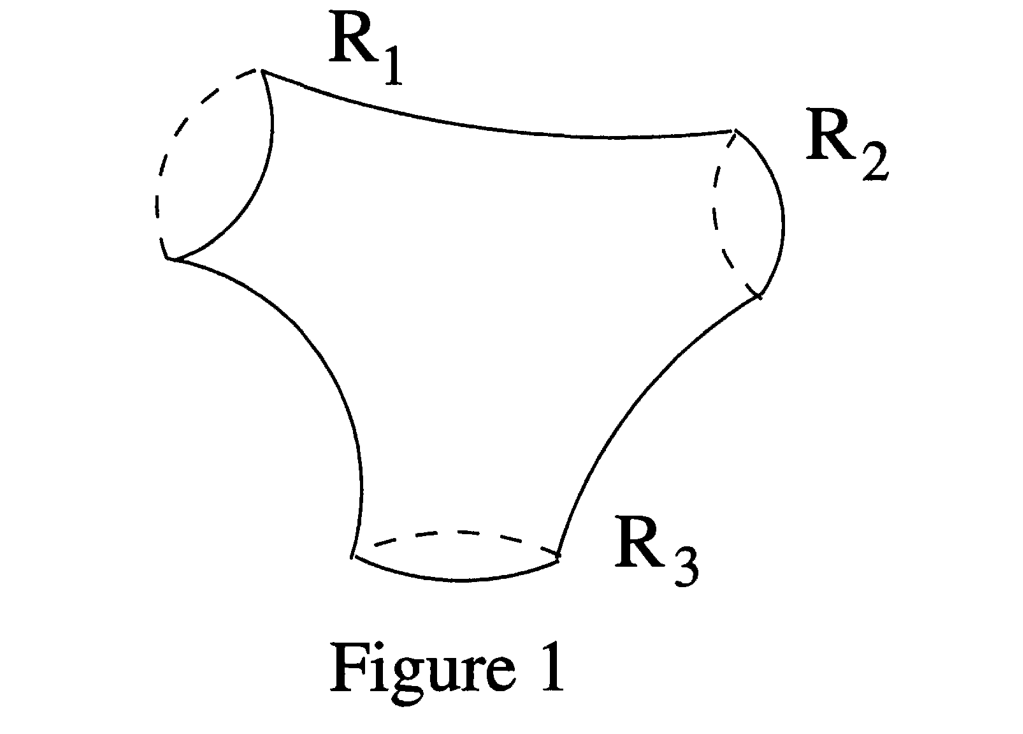
\includegraphics[width=0.52\textwidth]{figs/fig_p154_1.png}
  \caption{三孔球面（trinion，亦称「裤子」）：由球面挖去三个圆盘得到，三条边界分支分别标记为 $R_1$、$R_2$、$R_3$（虚线表示被挖去的圆盘的边沿）。（原文 Figure 1，p.154）}
  \label{fig:p154-1}
\end{figure}

我们设想在 $\mathcal{P}$ 上作路径积分，并在各边界分支上插入态 $\Psi_{R_i}$（$i=1,2,3$）。这个路径积分是
\begin{equation}
  \tag{11.33}
  \label{eq:11-33}
  W_{R_1R_2R_3}=\int \mathcal{D}A\,\exp(-\mathcal{L})\prod_{i=1}^{3}\Psi_{R_i}(A|_{C_i}),
\end{equation}

% ===== 原文 p.155 =====
其中 $A$ 取遍 $\mathcal{P}$ 上丛的联络空间。对任意的 $R_i$ 算出这个路径积分之后，把各部分拼装起来就相当直接了。

第一步是证明：除非诸 $R_i$ 全都相同，路径积分 $W_{R_1R_2R_3}$ 为零。我们在 $\mathcal{P}$ 中的某点 $p$ 处插入与可观测量 $Q_S^{(0)}(p)$ 相应的算符 $\widehat{Q_S^{(0)}}(p)$。我们假定 $p$ 靠近某个以表示 $R$ 标记的边界分支（$R$ 是诸 $R_i$ 之一）。于是可以认为算符 $\widehat{Q_S^{(0)}}(p)$ 作用在态 $\Psi_R$ 上。（这一点已在图 2（原文 Figure 2）中示意：那里算符插入被标记为 $S(F)$，并被看作作用在态 $\Psi_{R_1}$ 上。）利用 (11.30) 及其对高阶 Casimir 算符的推广，我们看到态 $\Psi_R$ 是 $\widehat{Q_S^{(0)}}(p)$ 的本征态，本征值为某个 $C(S,R)$：
\begin{equation}
  \tag{11.34}
  \label{eq:11-34}
  \widehat{Q_S^{(0)}}(p)\Psi_R=C(S,R)\Psi_R .
\end{equation}

\begin{figure}[htbp]
  \centering
  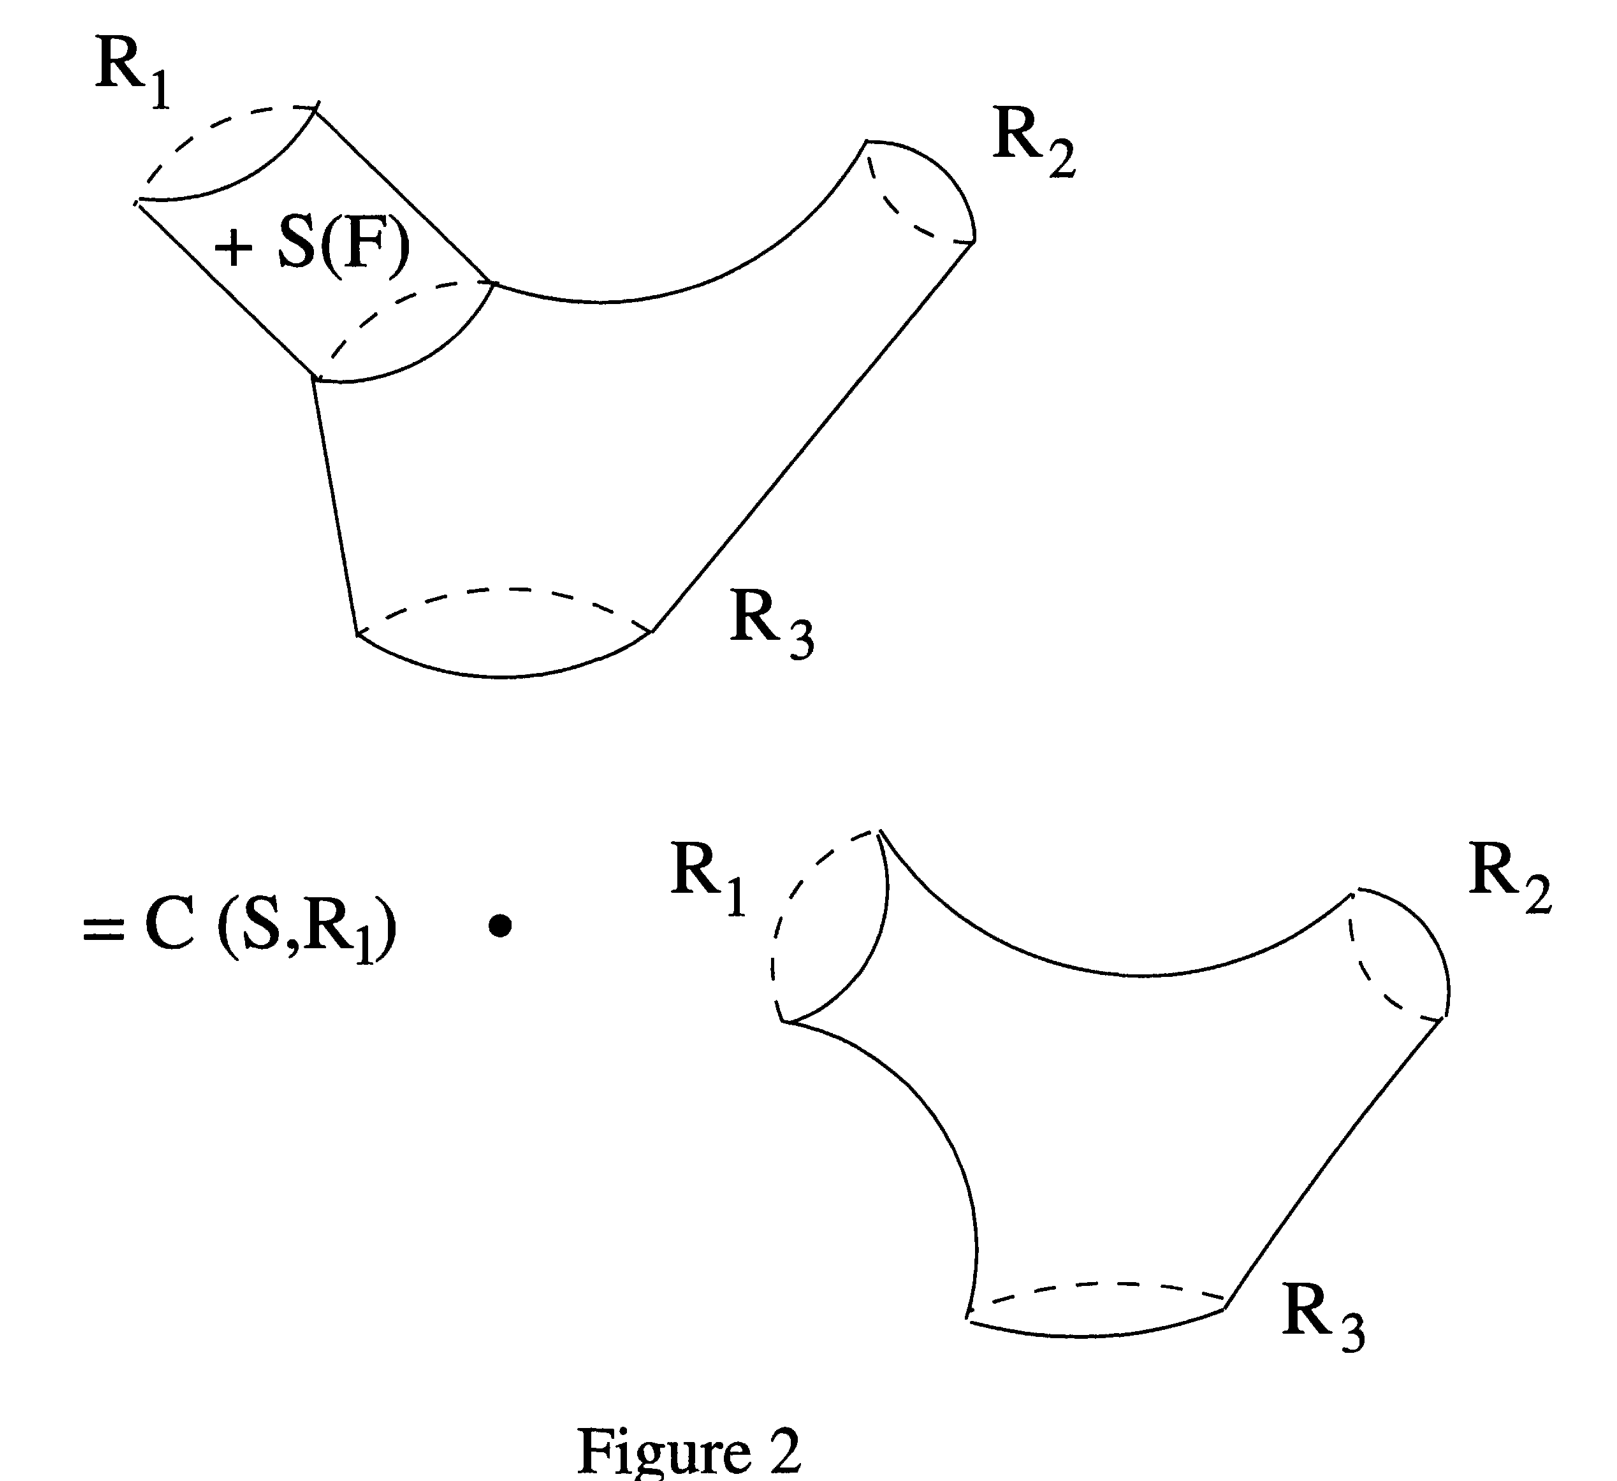
\includegraphics[width=0.60\textwidth]{figs/fig_p154_2.png}
  \caption{在 $R_1$ 所标记的边界分支附近插入算符（图中标为 $+S(F)$）的三孔球面路径积分，等于常数 $C(S,R_1)$ 乘以未插入算符的三孔球面路径积分（图中圆点表示乘法）。（原文 Figure 2，p.154）}
  \label{fig:p154-2}
\end{figure}

这里，若 $S$ 是 $\mathfrak{g}$ 上次数为 $l$ 的不变多项式，则 $C(S,R)$ 就是表示 $R$ 相应的 $l$ 阶 Casimir。（例如，若 $S$ 是规范不变函数 $S(\phi)=\mathrm{Tr}(\phi^{l})$，其中 $\mathrm{Tr}$ 取在伴随表示上，则量子化后 $S$ 成为 $\mathrm{Tr}(\delta/\delta A)^{l}$ 的某个倍数。$\Psi_R$ 是此算符的本征态，本征值为 $C(S,R)$ 的某个倍数。）由于 $R$ 可以取 $R_1$、$R_2$ 或 $R_3$ 中的任何一个，我们发现这个单点函数等于 $C(S,R_j)W_{R_1R_2R_3}$（$j=1,2,3$），其中 $W_{R_1R_2R_3}$ 如上定义。这一论断成立的理由如下：由于该场论在保面积微分同胚（area preserving diffeomorphism）下不变，我们可以把算符插入放在我们所选定的任何一条边界分支附近，因此该算符可以被看作作用在任何一个外态上。由此可见，对每个 $j$，Casimir 值 $C(S,R_j)$ 全都相等；又因这对所有不变多项式 $S$ 都成立，故只要 $W(R_1,R_2,R_3)\neq0$，就必须有 $R_1=R_2=R_3$。

% [Tutor Note: 由 (11.30) 到 (11.34) 的关键是把 $\phi^{a}$ 换成泛函导数 $\delta/\delta A^{a}$（见 p.153 的 (11.29)），于是 $S(\phi)=\mathrm{Tr}(\phi^{l})$ 量子化后确实是一个 $l$ 阶线性微分算符 $\mathrm{Tr}(\delta/\delta A)^{l}$。诸 $\delta/\delta A^{a}(x)$ 彼此对易，故此处无算符排序歧义——但也正因如此，$\Psi_R$ 是真正的本征态而不仅是广义本征态。易错点：式中的 $\mathrm{Tr}$ 必须取在伴随表示上（原文如此）；若误取基本表示，$C(S,R)$ 就不再是 $R$ 的 Casimir 而是别的缩并，于是「三个边界分支的 Casimir 相等 $\Rightarrow R_1=R_2=R_3$」这一步失效。]

于是问题归结为计算 $\mathcal{P}$ 的配分函数，其边界条件由三条边界分支上同一个外态 $\Psi_R$ 决定。把这个配分函数在零面积极限下的值记为 $w_R$。那么面积依赖关系是：若面积为 $a$，则得到
\begin{equation}
  \tag{11.35}
  \label{eq:11-35}
  Z_R=w_R\exp\left(-\tilde{c}_2(R)\frac{ae^{2}}{2}\right),
\end{equation}
这里我们现用 $Z_R$ 表示 $W_{R,R,R}$。面积依赖关系必定如此，理由是我们可以在任一边界分支上粘上一个给定面积的圆柱来增大三孔球面的面积；这会把 $Z_R$ 乘以在把 $\Psi_R$ 沿给定面积传播时出现的因子 (11.31)。

% [Tutor Note: (11.35) 中出现的是 $\tilde{c}_2$ 而非 $c_2$，这不是笔误，而是 (11.32) 重整化效应的体现：$\tilde{c}_2(R)=c_2(R)+\beta$，常数移位 $\beta$ 在 (11.35) 里给出一个与 $R$ 无关的因子 $e^{-e^{2}a\beta/2}$，可并入 $w_R$；p.160 的 $c_2(R_n)=(n^{2}-1)/2\to\tilde{c}_2(R_n)=n^{2}/2$ 正是 $\beta=1/2$。另外要看清「面积依赖只能是这一个指数」的真正依据：圆柱传播子 (11.31) 只含 $e^{-e^{2}a\,c_2/2}$ 一个因子，故 $\ln Z_R$ 对 $a$ 必须是线性的，这就排除了 $\ln Z_R$ 中出现 $a^{2}$ 等高次项的可能——等价地说，二维 Yang--Mills 是超可重整化理论，作用量中可用的一次项只有 $\int\mathrm{tr}\,F^{2}$ 与 $\int R$（后者见 (11.32)）。]

现在我们来考虑亏格为 $g$、无边界 Riemann 面的配分函数的计算问题。这样的曲面可以由 $2g-2$ 个 $\mathcal{P}$ 的副本 $\mathcal{P}_j$ 沿 $3g-3$ 条边界圆 $C_\gamma$ 粘合而成。我们可以按场在边界圆 $C_\gamma$ 上的限制值来分解配分函数的路径积分。若 $A'$ 表示诸 $\mathcal{P}_j$ 的边界圆 $\coprod_\gamma C_\gamma$ 上一个联络的取值，而 $\mathcal{A}_{A'}=\{A\in\mathcal{A}:\ A|_{\coprod_\gamma C_\gamma}=A'\}$ 是

% ===== 原文 p.156 =====
所有限制到给定边界值 $A'$ 的联络之集合，则我们有\footnote[3]{见本讲末尾参考文献中所列 Witten 第一篇论文的 §4.5。}
\begin{equation}
  \tag{11.36}
  \label{eq:11-36}
  \int_{\mathcal{A}}\mathcal{D}A\,e^{-\mathcal{L}}=\int \mathcal{D}A'\int_{\mathcal{A}_{A'}}\mathcal{D}A\,e^{-\mathcal{L}} .
\end{equation}
这里，右端的 $DA$ 是对那些在诸 $C_\gamma$ 上限制为 $A'$ 的 $A$ 所作的积分。一旦固定了诸 $C_\gamma$ 上的联络 $A'$，空间 $\mathcal{A}_{A'}$ 就是 $2g-2$ 个 $\mathcal{P}$ 上联络空间（带指定的边界值）的乘积。$\mathcal{P}$ 在给定联络边界值与面积 $a$ 下的配分函数为
\begin{equation}
  \tag{11.37}
  \label{eq:11-37}
  Z(\mathcal{P},A|_{\partial\mathcal{P}})=\sum_{R}w_R\prod_{\gamma=1}^{3}\Psi_R(A|_{C_\gamma})\exp\left(-\frac{e^{2}a\tilde{c}_2(R)}{2}\right).
\end{equation}
（鉴于诸 $\Psi_R$ 的正交性，这与 (11.35) 等价。）要还原亏格 $g$ 的闭 Riemann 面 $\Sigma$ 的配分函数，我们把 $2g-2$ 个 $Z(\mathcal{P})$ 相乘并对边界值 $A'$ 积分。利用与诸态 $\Psi_R$ 相对应的群特征标的正交关系，我们得知：只有当 $2g-2$ 个三孔球面中每一个上面的诸 $R$ 全都相同时，才出现非零贡献。对 $R$ 求和给出
\begin{equation}
  \tag{11.38}
  \label{eq:11-38}
  Z(\Sigma)=\sum_{R}w_R^{2g-2}\exp\left(-\frac{e^{2}a\tilde{c}_2(R)}{2}\right).
\end{equation}
（当然，此时 $a$ 是整个曲面的面积。）

现在我们来解释如何计算 $w_R$。我们注意到，面积为 $a$、边界上有外态 $\Psi_R$ 的圆盘 $D$ 的配分函数是
\begin{equation}
  \tag{11.39}
  \label{eq:11-39}
  Z_R(D)=v_R\exp\left(-\frac{e^{2}a\tilde{c}_2(R)}{2}\right),
\end{equation}
其中 $v_R$ 为某个常数。面积依赖关系由通常的因子给出，因为同样地，我们可以通过给边界粘上一个给定面积的圆柱来改变面积。

边界条件由两个边界分支上的波函数 $\Psi_R$（相应地 $\Psi_{R'}$）所决定的圆柱，其配分函数当 $R\neq R'$ 时等于 $0$，因为 $\Psi_R$ 是 Hamilton 量 $H$ 的本征函数。（见

\begin{figure}[htbp]
  \centering
  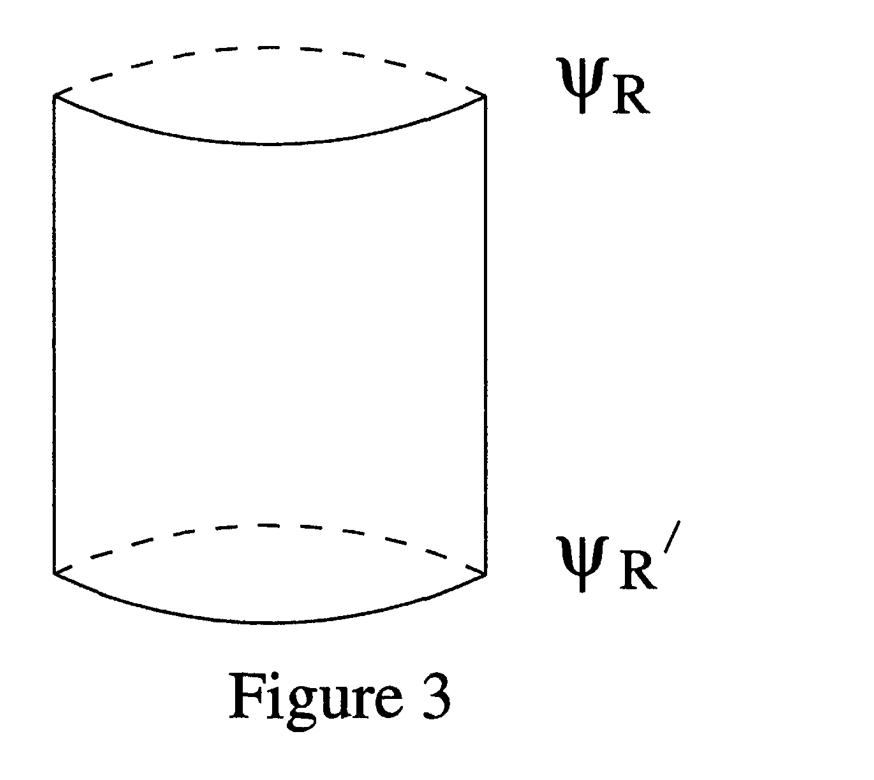
\includegraphics[width=0.40\textwidth]{figs/fig_p156_1.png}
  \caption{圆柱 $S^{1}\times I$：两个边界分支上分别带有外态 $\Psi_R$（上）与 $\Psi_{R'}$（下）。当 $R\neq R'$ 时其配分函数为零。（原文 Figure 3，p.156）}
  \label{fig:p156-1}
\end{figure}

% ===== 原文 p.157 =====
图 3。）面积为 $a$、两个边界分支上都有外态 $\Psi_R$ 的圆柱 $S^{1}\times I$ 的配分函数为
\begin{equation}
  \tag{11.40}
  \label{eq:11-40}
  Z_R(S^{1}\times I)=1\cdot\exp\left(-\frac{e^{2}a\tilde{c}_2(R)}{2}\right)
\end{equation}
（因为诸 $\Psi_R$ 是 Hamilton 量 $H$ 的本征态，而圆柱上的路径积分计算的是 $e^{-HT}$；注意，由于其 Hamilton 量解释，这个公式与前面几个公式不同，不含任何未知的乘性常数）。我们可以像图 4（原文 Figure 4）那样分解圆柱：这给出「两个边界分支上都有外态 $\Psi_R$ 的圆柱」的配分函数，它等于「所有边界分支上都有外态 $\Psi_R$ 的 $\mathcal{P}$」的配分函数与 $D$ 的配分函数之积，于是
\begin{equation}
  \tag{11.41}
  \label{eq:11-41}
  w_R\cdot v_R=1 .
\end{equation}
要确定 $v_R$，只需考虑面积非常小的圆盘 $D$。若把 $D$ 边界上一个联络的和乐（holonomy）固定为取值 $U\in G$，则圆盘的配分函数（限制到 $D$ 上边界和乐为 $U$ 的联络）为（由 (11.39) 并利用特征标的正交性）
\begin{equation}
  \tag{11.42}
  \label{eq:11-42}
  Z(U)=\sum_{R}v_R\chi_R(U)\exp\left(-\frac{e^{2}a\tilde{c}_2(R)}{2}\right)
\end{equation}
（其中 $\chi_R$ 如上所述，表示 $R$ 的特征标）。如果我们改用路径积分来计算配分函数，则把作用量写成
\begin{equation}
  \tag{11.43}
  \label{eq:11-43}
  I(U)=\frac{1}{4e^{2}}\int_D d\mu\,\mathrm{Tr}(|F|^{2}),
\end{equation}
以及
\begin{equation}
  \tag{11.44}
  \label{eq:11-44}
  Z(U)=\int_{\mathrm{Hol}(A)=U}\mathcal{D}A\,\exp\left(-\frac{1}{4e^{2}}\int_D d\mu\,\mathrm{Tr}(|F|^{2})\right),
\end{equation}
（其中我们限制到边界和乐为 $U$ 的联络）。这个积分给出 $U$ 的一个正函数，因为被积函数是正的。当 $e^{2}$（等价地，面积）趋于零时，$Z(U)$ 的支集收敛到 $U=1$，因为任何和乐固定为 $U\neq1$ 的构型，其作用量当 $e\to0$ 时都发散。因此当 $e\to0$ 时，该积分收敛到支撑在 $U=1$ 处的 delta 函数。这给出
\begin{equation}
  \tag{11.45}
  \label{eq:11-45}
  Z(U)=\exp(\alpha)\cdot\delta(U-1),
\end{equation}
这里 $\alpha$ 是一个迄今未知的常数。我们将会看到，它本质上就是 (11.32) 中乘在 Riemann 面 Euler 示性数上的那个常数。把 (11.44) 与 (11.41) 的 $e\to0$ 极限作比较，我们看到
\begin{equation}
  \tag{11.46}
  \label{eq:11-46}
  \exp(\alpha)\delta(U-1)=\sum_{R}v_R\chi_R(U).
\end{equation}
若把此式两端乘以 $\chi_{R'}(U)$ 并对 $U$ 积分，利用群特征标的正交关系，我们得到
\begin{equation}
  \tag{11.47}
  \label{eq:11-47}
  v_R=\exp(\alpha)\dim R,
\end{equation}
从而
\begin{equation}
  \tag{11.48}
  \label{eq:11-48}
  w_R=\frac{\exp(-\alpha)}{\dim R}.
\end{equation}

% [Tutor Note: 原文「Comparing (11.44) to the $e\to0$ limit of (11.41)」中的 (11.41) 应为 (11.42)。(11.41) 是纯数等式 $w_Rv_R=1$，与 $U$ 无关，无法与 (11.44) 相比较；只有 (11.42) 在 $e\to0$（指数因子 $\to1$）时化为 $\sum_R v_R\chi_R(U)$，才与 (11.45) 的 $\exp(\alpha)\delta(U-1)$ 相等，从而得到 (11.46)。此处按原文照译并加注。]

% [Tutor Note: (11.46)$\to$(11.47) 用的是 Peter--Weyl 关系 $\delta(U-1)=\sum_R(\dim R)\chi_R(U)$ 与 $\int dU\,\chi_R(U)\chi_{R'}(U)=\delta_{RR'}$（Haar 测度取归一化 $\int dU=1$）。由此 $v_R=e^{\alpha}\dim R$，再配合 (11.41) 得 $w_R=e^{-\alpha}/\dim R$。易错点：若把 $\chi_R$ 换成归一化特征标 $\hat\chi_R=\chi_R/\dim R$（作者在 (11.53)、(11.55) 中正是用 $\hat\chi_R$），则 delta 函数的展开须写成 $\delta(U-1)=\sum_R(\dim R)^{2}\hat\chi_R(U)$，否则 (11.47)、(11.48) 中的 $\dim R$ 因子会整体错位。]

% ===== 原文 p.158 =====
\begin{figure}[htbp]
  \centering
  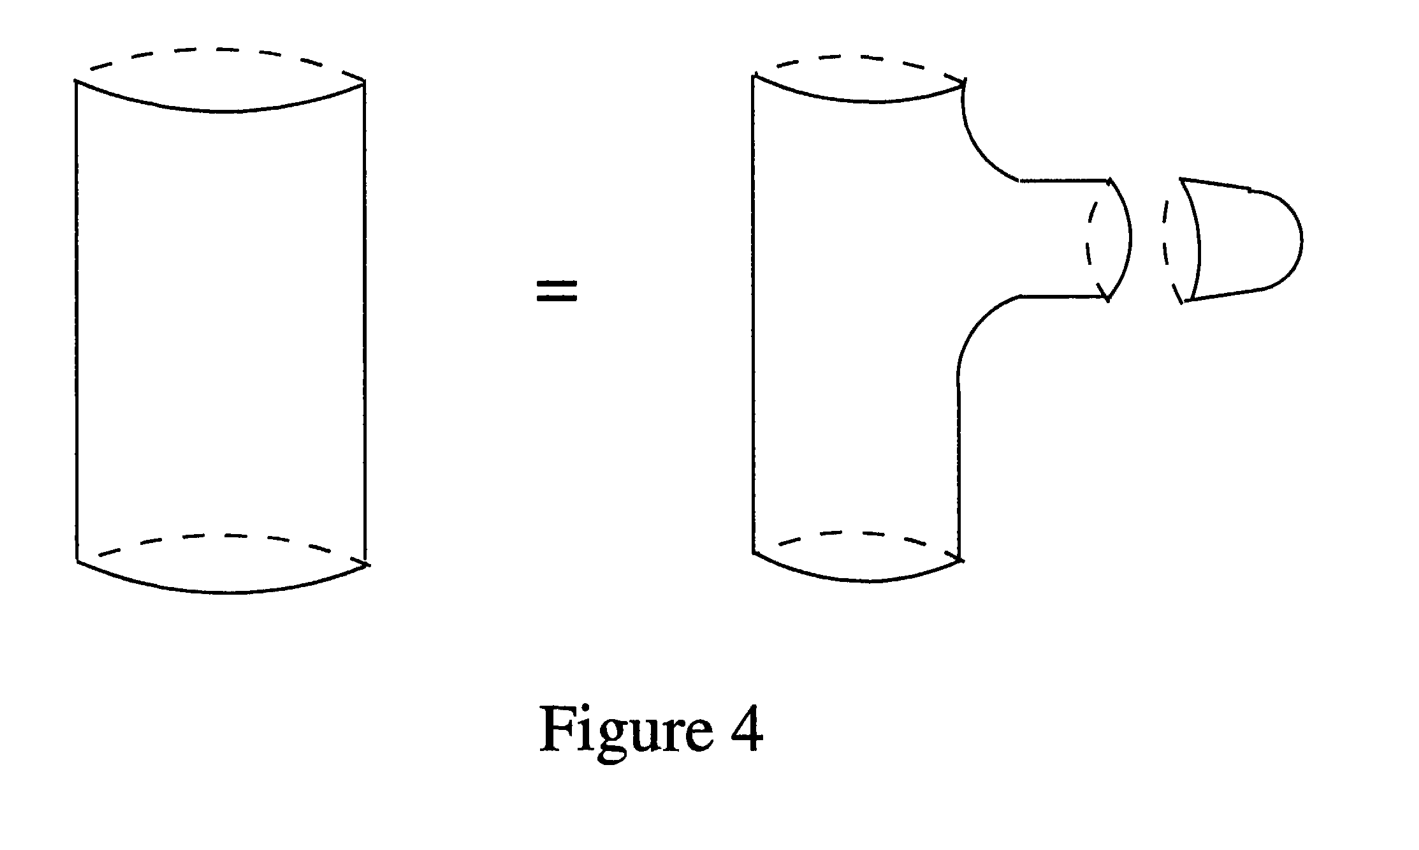
\includegraphics[width=0.62\textwidth]{figs/fig_p158_1.png}
  \caption{圆柱的分解：圆柱 $=$ 三孔球面 $\mathcal{P}$（左）与圆盘 $D$（右）沿一条边界圆粘合；等式表示两边配分函数相乘。（原文 Figure 4，p.158）}
  \label{fig:p158-1}
\end{figure}

于是配分函数为
\begin{align}
  \tag{11.49}
  \label{eq:11-49}
  Z(\Sigma^{g},e^{2}a)&=\sum_{R}w_R^{2g-2}\exp\left(-\frac{\tilde{c}_2(R)e^{2}a}{2}\right)\\
  \tag{11.50}
  \label{eq:11-50}
  &=\sum_{R}\frac{e^{-\alpha(2g-2)}\exp\left(-\tilde{c}_2(R)\varepsilon/2\right)}{(\dim R)^{2g-2}},
\end{align}
其中我们引入了 $\varepsilon=e^{2}a$。

我们刚刚完成的计算给出的是对应于所有可能拓扑类型的 $G$-丛的配分函数之和（回忆一下：若 $G$ 不是单连通的，则 $\Sigma$ 上一般会有若干不同拓扑类型的丛）。要研究某一个特定拓扑类型的贡献，我们取 $G$ 为单连通，并选取一个元素 $\zeta\in Z(G)$（$G$ 的中心）。在 $\Sigma$ 上选一点 $p$，我们限制到 $\Sigma-\{p\}$ 上绕 $p$ 的和乐等于 $\zeta$ 的那些联络。这样的联络会下降为结构群是 $G/Z(G)$ 的商丛上的光滑联络，其拓扑由 $\zeta$ 决定。我们即将大量使用「$G$-丛上具有所述类型奇性的联络」与「$G/Z(G)$-丛上的光滑联络」之间的这一关系。

要把计算推广到带这类奇性的 $G$-丛，我们需要算出包含奇点 $p$（绕 $p$ 的规定单值性（monodromy）为 $\zeta$）的小圆盘 $D$ 上的配分函数，把它表示为圆盘边界上绕行和乐 $U$ 的函数。然后，把 $D$ 粘进任意 Riemann 面，我们就得到该 Riemann 面在包含奇点 $p$ 时的配分函数。在 $e\to0$ 极限下，$D$ 上的配分函数（通过量子化）由
\begin{equation}
  \tag{11.51}
  \label{eq:11-51}
  \sum_{R}u_R\chi_R(U)
\end{equation}
给出，其中 $u_R$ 未知；而（通过路径积分）由
\begin{equation}
  \tag{11.52}
  \label{eq:11-52}
  \exp(\alpha)\delta(U-\zeta)
\end{equation}
给出。后一论断的依据是：若绕 $p$ 的单值性是 $\zeta$，但绕圆盘边界的单值性为 $U\neq\zeta$，则路径积分中的最小作用量在 $e\to0$ 时发散，路径积分将为零；因此该路径积分在 $e\to0$（或小面积）极限下是 $\delta(U-\zeta)$ 的正倍数。

% ===== 原文 p.159 =====
若我们乘以 $\chi_{R'}(U)$ 并对 $U$ 积分，则由特征标的正交性可得
\begin{equation}
  \tag{11.53}
  \label{eq:11-53}
  u_R=\exp(\alpha)\chi_R(\zeta)=\exp(\alpha)(\dim R)\hat{\chi}_R(\zeta),
\end{equation}
其中 $\hat{\chi}_R(\zeta)\in U(1)$ 是表示 $R$ 的归一化特征标在 $\zeta$ 处的取值。现在，若把 $2g-1$ 个 $\mathcal{P}$ 的副本与一个圆盘 $D$ 粘合起来，构成亏格为 $g$ 的闭 Riemann 面，则对配分函数我们得到
\begin{align}
  \tag{11.54}
  \label{eq:11-54}
  Z(\varepsilon,g,\zeta)&=\sum_{R}w_R^{2g-1}e^{-\tilde{c}_2(R)e^{2}a/2}u_R\\
  \tag{11.55}
  \label{eq:11-55}
  &=\sum_{R}\frac{e^{-\alpha(2g-2)}e^{-\varepsilon\tilde{c}_2(R)/2}}{(\dim R)^{2g-2}}\hat{\chi}_R(\zeta).
\end{align}
这是亏格 $g$、带一个穿刺点（puncture）、且绕该穿刺点的和乐为 $\zeta$ 的 Riemann 面上 $G$-联络的配分函数。而我们想要的是相应的 $G/Z(G)$-丛上光滑 $G/Z(G)$-联络的配分函数，该丛的特征类由 $\zeta$ 决定。

% [Tutor Note: 「用 $2g-1$ 个 $\mathcal{P}$ 加一个 $D$ 拼成亏格 $g$ 的闭曲面」可用 Euler 示性数核对：$\chi(\mathcal{P})=2-3=-1$，$\chi(D)=1$，粘合不改变 $\chi$，故总数 $\chi=-(2g-1)+1=2-2g$，正是亏格 $g$ 闭曲面的值；作为对照，无穿刺情形用 $2g-2$ 个 $\mathcal{P}$，$\chi=-(2g-2)=2-2g$。再核对 (11.55) 的幂次：$w_R^{2g-1}u_R=(e^{-\alpha}/\dim R)^{2g-1}\cdot e^{\alpha}(\dim R)\hat\chi_R=e^{-\alpha(2g-2)}\hat\chi_R/(\dim R)^{2g-2}$，与 (11.55) 完全吻合。]

正如我们已经指出的，在「$G$-丛上绕穿刺点 $p$ 单值性为 $\zeta$ 的联络空间」与「拓扑类型由 $\zeta$ 决定的 $G/Z(G)$-丛上的联络空间」之间存在自然的等同。然而，两者的规范群——从而它们的体积——是不同的。设 $\widetilde{G}_1$ 是单值性为 $\zeta$（绕 $p$）的 $G$-丛上的规范变换群，$\widetilde{G}_2$ 是相应的 $G/Z(G)$-丛上的规范变换群。$\widetilde{G}_2$ 有一个指数为 $(\#Z(G))^{2g}$ 的子群（由那些沿 $\Sigma$ 中的圈走一圈、从 $G/Z(G)$ 提升到 $G$ 之后为单值的规范变换组成），它同构于 $\widetilde{G}_1$ 模去其中心所得的商（$\widetilde{G}_1$ 的中心是由 $G$ 的中心元素所作的常规范变换构成的群，阶为 $\#Z(G)$）。于是 $\mathrm{Vol}\,\widetilde{G}_2=\#Z(G)^{2g-1}\,\mathrm{Vol}\,\widetilde{G}_1$，从而拓扑类型由 $\zeta$ 决定的 $G/Z(G)$-丛的配分函数，可由 (11.55) 除以因子 $(\#Z(G))^{2g-1}$ 得到。

% [Tutor Note: 这里的体积因子指数是 $(\#Z(G))^{2g-1}$ 而不是 $2g$，极易算错：$\widetilde{G}_2$ 含一个指数为 $(\#Z(G))^{2g}$ 的子群 $H\cong\widetilde{G}_1/Z(\widetilde{G}_1)$，而 $\widetilde{G}_1\to\widetilde{G}_1/Z(\widetilde{G}_1)$ 本身又是 $\#Z(G)$ 重覆盖，故 $\mathrm{Vol}\,\widetilde{G}_2=(\#Z(G))^{2g}\mathrm{Vol}\,\widetilde{G}_1/\#Z(G)=(\#Z(G))^{2g-1}\mathrm{Vol}\,\widetilde{G}_1$。这也解释了 (11.56) 的形式：从 (11.55) 除以 $2^{2g-1}$（$Z(SU(2))=\mathbb{Z}_2$）只留下与 $g$ 有关的因子 $2^{-(2g-2)}=e^{-(2g-2)\ln2}$，它可并入 $e^{-\alpha(2g-2)}$，而剩下那个 $1/2$ 正是原文所说「与亏格无关的整体常数」。]

这样我们就得到了物理 Yang--Mills 理论在任意指定拓扑类型的 $G/Z(G)$-丛上的配分函数。§11.4 的论证把这个积分表达为辛商（symplectic quotient）上的相交理论。在目前的情形下，辛商就是给定拓扑类型的光滑全纯稳定 $G/Z(G)$-丛的模空间。因此，我们理应得到该模空间上相交理论的公式。若更仔细地重审 §11.4 的讨论，就会清楚：即使在有限维情形，「把积分等同于辛商上的相交理论」这一断言也只在辛商光滑时才成立。否则得到的是更复杂的陈述（至今研究不多），其中奇性会进入。就模空间上相交理论的应用而言，模空间光滑的情形是：$G/Z(G)=SU(N)/\mathbb{Z}_n$，$\zeta$ 是 $\mathbb{Z}_n$ 的生成元，且亏格大于 $1$；此时模空间就是秩为 $n$、第一 Chern 类与 $n$ 互素的全纯向量丛的模空间。该模空间上的相交理论由一些公式支配，这些公式可以由上面配分函数的计算与 §11.4 的局部化结果结合起来得到。我们不会真的把这些公式写出来；精确的陈述（以及不借助量子场论的严格证明）见参考文献。在 $G/Z(G)$ 不是 $SU(n)/\mathbb{Z}_n$（或 $\zeta$ 不是 $\mathbb{Z}_n$ 的生成元）的情形，处境类似于四维的 Donaldson 理论。

% [Tutor Note: 原文此处写作 $SU(N)/\mathbb{Z}_n$，而同一句后文与全段的用法（秩 $n$、第一 Chern 类与 $n$ 互素）表明应为 $SU(n)/\mathbb{Z}_n$：因为 $Z(SU(N))=\mathbb{Z}_N$，若群是 $SU(N)$ 而商的是 $\mathbb{Z}_n$（$n\neq N$），$\mathbb{Z}_n$ 并不是 $SU(N)$ 的中心子群，「商群」无意义。这是原文的一处符号不一致，翻译时照录并加注。]

% ===== 原文 p.160 =====
四维的 Donaldson 理论。给定类型的全纯 $G/Z(G)$-丛的模空间带有奇性，因此相交理论没有唯一定义。不过，在某个「稳定」范围内，可以定义一些相交数，同时避开奇性。这些相交数应当由上面 Yang--Mills 配分函数的公式确定；但这同样尚未在数学上得到研究。

我们以 $G=SU(2)$、$\zeta=-1$ 这个例子来结束本节，这是全纯丛的模空间光滑的第一个情形。对每个整数 $n\ge1$，存在唯一的 $n$ 维不可约表示 $R_n$；它有 $\hat{\chi}_n(\zeta)=(-1)^{n+1}$。表示 $R_n$ 的二次 Casimir 为
\[
  c_2(R_n)=(n^{2}-1)/2;
\]
它被重整化为
\[
  \tilde{c}_2(R_n)=n^{2}/2.
\]
对应于 $w_2\neq0$ 的 $SO(3)$ 丛（$w_2$ 为第二 Stiefel--Whitney 类）的配分函数为（在相差一个与亏格 $g$ 无关的整体乘性归一化常数的意义下）
\begin{equation}
  \tag{11.56}
  \label{eq:11-56}
  Z(\varepsilon)=e^{-\alpha(2g-2)}\sum_{n\ge1}\frac{(-1)^{n+1}}{n^{2g-2}}e^{-\varepsilon n^{2}/4}.
\end{equation}
现在让我们验证：它是一项关于 $\varepsilon$ 的多项式（若 $Z(\varepsilon)$ 确实决定了模空间上的相交理论，则由 (11.21) 应预期这种多项式依赖）与另一项之和，后者按 $e^{-b/\varepsilon}$ 的量级指数衰减（$b$ 为某个正常数），并反映了更高临界点的贡献——按参考文献中所引 Atiyah 与 Bott 的结果，这些临界点对应于不稳定的全纯丛。我们通过对该级数求导来做到这一点，得到
\begin{equation}
  \tag{11.57}
  \label{eq:11-57}
  e^{\alpha(2g-2)}4^{g-1}\left(\frac{\partial}{\partial\varepsilon}\right)^{g-1}Z(\varepsilon)=F(\varepsilon),
\end{equation}
其中我们定义
\[
  F(\varepsilon)=\sum_{n\ge1}(-1)^{n+1}e^{-\varepsilon n^{2}/4}.
\]
我们有
\[
  2F(\varepsilon)-1=-\sum_{n\in\mathbb{Z}}(-1)^{n}e^{-\varepsilon n^{2}/4},
\]
而利用 Poisson 求和公式，它由下式给出
\begin{equation}
  \tag{11.58}
  \label{eq:11-58}
  2F(\varepsilon)=1-\sqrt{4\pi/\varepsilon}\sum_{m\in\mathbb{Z}}\exp\left(-(2\pi)^{2}(m+1/2)^{2}/\varepsilon\right).
\end{equation}
（求和中以 $m$ 编号的项，对应于 Yang--Mills 泛函由形如 $\mathcal{L}_m\oplus\mathcal{L}_{-m+1}$ 的不稳定丛所产生的临界点的贡献，其中 $\mathcal{L}_m$ 是 $\Sigma$ 上次数为 $m$ 的线丛。）现在我们可以应用 (11.57) 来积分 (11.58)，从而说明 $Z(\varepsilon)$ 是一个关于 $\varepsilon$ 的多项式（次数为 $g-1$）与一个按 $e^{-b/\varepsilon}$ 指数衰减的项之和，$b$ 为某个正常数。若考虑第一 Chern 类平凡的秩二丛，我们只需在配分函数中略去因子 $(-1)^{n+1}$。在此情形下，同类的分析表明：$Z(\varepsilon)$ 有一个按 $\varepsilon$ 的整数幂的展开，直到某一阶为止，此后出现一项带半整数指数的项。$Z(\varepsilon)$ 不能写成

% [Tutor Note: (11.57) 左端疑似漏了因子 $(-1)^{g-1}$。逐项对 (11.56) 求导：每次 $\partial_\varepsilon$ 作用在 $e^{-\varepsilon n^{2}/4}$ 上给出因子 $-n^{2}/4$，共作用 $g-1$ 次，遂得 $(\partial_\varepsilon)^{g-1}Z=e^{-\alpha(2g-2)}(-1)^{g-1}4^{-(g-1)}F(\varepsilon)$，即左端应带 $(-1)^{g-1}4^{g-1}$。由于 $(-1)^{g-1}=e^{i\pi(g-1)}$ 恰可由常数平移 $\alpha\to\alpha-i\pi/2$ 吸收（因 $(2g-2)\cdot i\pi/2=i\pi(g-1)$），(11.57) 在「$\alpha$ 尚未固定」的意义下成立；但若沿用 (11.55) 中已确定的 $\alpha$，则此处漏掉一个符号。]

% [Tutor Note: (11.58) 中的 $(m+1/2)$ 来自 $(-1)^{n}=e^{i\pi n}$：Poisson 求和把 $\sum_n e^{-\varepsilon n^{2}/4+i\pi n}$ 化为对偶格上的高斯和，对偶格矢因此被平移 $1/2$。若漏掉 $(-1)^{n}$（例如讨论第一 Chern 类平凡的秩二丛时），得到的是 $\sum_m e^{-4\pi^{2}m^{2}/\varepsilon}$，衰减率随之改变。按 (11.58)，$m=0$ 与 $m=-1$ 两项给出 $b=(2\pi)^{2}(1/2)^{2}=\pi^{2}$，即 $Z(\varepsilon)$ 的指数小修正为 $O(e^{-\pi^{2}/\varepsilon})$ 量级——作者只写「某个正常数 $b$」而未给数值，这个数值可以这样补出。]

% ===== 原文 p.161 =====
「多项式加指数小修正」的形式，这一点反映了第一 Chern 类平凡的秩二丛的模空间的奇性。

\subsection*{参考文献与交叉引用}

本讲的一些基本参考文献是
\begin{itemize}
  \item A.A. Migdal, Sov. Phys. JETP \textbf{42}, 413 (1975)（Zh. Eksp. Teor. Fiz. \textbf{69}, 810 (1975)）。
  \item E. Witten, On quantum gauge theories in two dimensions, \emph{Commun. Math. Phys.} \textbf{141} (1991) 153--209.
  \item E. Witten, Two dimensional gauge theories revisited, hep-th/9204083; \emph{J. Geom. Phys.} \textbf{9} (1992) 303--368.
\end{itemize}

两维的 Yang--Mills 理论在前两篇中得到分析，而用全纯丛模空间上的相交理论所作的解释则在第三篇中得到发展。利用 Cartan 模型对局部化与等变上同调所作的数学处理可见于
\begin{quote}
  N. Berline, E. Getzler, M. Vergne, \emph{Heat Kernels and Dirac Operators}, Springer-Verlag (Grundlehren vol. 298), 1992.
\end{quote}

Cartan 模型中等变积分的数学处理可见于
\begin{quote}
  L. Jeffrey, F. Kirwan, Localization for nonabelian group actions, \emph{Topology} \textbf{34} (1995) 291--327.
\end{quote}

模空间 $\mathcal{M}$、特别是其上同调，在下列文献中讨论：
\begin{quote}
  M.F. Atiyah, R. Bott, The Yang--Mills equations over Riemann surfaces, \emph{Phil. Trans. Roy. Soc. Lond.} \textbf{A 308} (1983) 523--615.
\end{quote}

对 $G=SU(2)$ 情形相交数公式的数学证明见
\begin{quote}
  M. Thaddeus, Conformal field theory and the cohomology of the moduli space of stable bundles, \emph{J. Diff. Geom.} \textbf{35} (1992) 131--149.
\end{quote}

该文还含有 §11.5 中论证的数学版本。对 $G=SU(n)$（在模空间 $\mathcal{M}$ 光滑的那些情形），相交数公式的证明见
\begin{quote}
  L. Jeffrey, F. Kirwan, Intersection pairings in moduli spaces of vector bundles of arbitrary rank over a Riemann surface, \emph{Ann. Math.} \textbf{148}(1) (1998), 109--196.
\end{quote}

§11.1 中的超对称变换与 §11.3 的下降方程（descent equations），将在第 14 讲中以更一般的框架重新讨论。


\clearpage
% 原文 pp.163–172（印刷 pp.1281–1290）
\section{Lecture 12：超对称场论}

\begin{keytakeaways}
本讲引入超对称（supersymmetry）场论：对称群非平凡地扩张为超群，其 Lie 超代数的奇元素给出费米型的无穷小对称。全讲的核心物理图像是：经典场方程的解若在某些（而非全部）超对称下不变，便自动在给定拓扑类中取能量的极小，这类解称为 BPS 态。核心数学工具是超空间（superspace）上的超场与超势（superpotential），以及把超对称条件化为一阶（Bogomolny 型）方程：在二维 $N=2$ 模型中，超对称孤子恰是超势 $W$ 的临界点之间沿 $h=\mathrm{Re}(e^{-i\alpha}W)$ 的梯度流线，其能量恰为 $|T|$，$T=W(\phi(\infty))-W(\phi(-\infty))$。四维 $N=1$、$N=2$ 的超庞加莱表示由相应 Clifford 代数二次型的秩决定（无质量表示维数 $2,4$，有质量表示维数 $4,16$），由此得到矢量多重态、手征多重态与超多重态等粒子内容。主要结论是：超对称代数可以含有中心荷（central charge），中心荷使 BPS 界 $M\ge|S|$ 能够被饱和；$N=2$ 规范理论中的中心荷必然是电荷与磁荷的线性组合，而质量恰等于 $|S|$ 的 BPS 磁单极子，是学期末研究 Seiberg--Witten 理论与 Donaldson 理论的出发点。
\end{keytakeaways}

% ===== 原文 p.163 =====
\subsection{超对称位形}
% 原文 §12.1：Supersymmetric Configurations

从今天起，我们研究具有超对称的场论，即其对称群可以非平凡地扩张为一个超群（supergroup）的场论。
按照惯例，所谓偶（even）与奇（odd）的（无穷小）对称，指的正是这个超群的 Lie 超代数（Lie superalgebra）中的偶元素与奇元素。

经常出现的情形是：经典场方程的一个解带有非平凡的奇对称。例如：

\begin{quote}
\noindent 梯度流线（gradient flow lines，Morse 理论中的）\\
\noindent 全纯曲线（holomorphic curves）\\
\noindent 规范理论瞬子（gauge theory instantons）\\
\noindent 磁单极子（monopoles）\\
\noindent Seiberg--Witten 解\\
\noindent 超 Kähler 结构（hyperKähler structures）\\
\noindent Calabi--Yau 度规\\
\noindent $G_2$ 与 $Spin_7$ 和乐的度规
\end{quote}

这些例子听起来差别很大，但它们有一个共同点：它们都是「在某些超对称下不变的经典场」的例子。
它们在数学上被大量研究，而在理解超对称量子系统的行为时也起着重要作用。

\subsection{超对称孤子（BPS 态）}
% 原文 §12.2：Supersymmetric solitons (BPS states)

首先考虑一个会出现 Morse 理论梯度流线的情形。
设 $h:\mathbb{R}^n\to\mathbb{R}$ 是 Morse 函数（即其临界点非退化，且 $|\nabla h|$ 在无穷远处增长）。Morse 函数总是只有有限多个临界点。
考虑（在闵可夫斯基号差下）映射 $\Phi:\mathbb{R}^{2|2}\to\mathbb{R}^n$ 的理论，其拉格朗日量为
\begin{equation}
  \tag{12.1}
  \label{eq:12-1}
  \mathcal{L}=\int d^2x\,d^2\theta\left(\frac12D_+\Phi D_-\Phi-h(\Phi)\right),
\end{equation}

\noindent\textit{（本讲笔记由 Pavel Etingof 与 David Kazhdan 整理。原文 p.163 页脚）}

% ===== 原文 p.164 =====
其中 $D_\pm=\dfrac{\partial}{\partial\theta_\pm}-\theta_\pm\partial_\pm$，$\partial_\pm=\dfrac{\partial}{\partial x^\pm}$，$x_\pm=\tfrac12(t\pm x)$。
此模型在 $Q_\pm=\dfrac{\partial}{\partial\theta_\pm}+\theta_\pm\partial_\pm$ 之下具有显然的超对称性。
这些超对称算符满足显然的对易关系 $Q_\pm^2=\partial_\pm$、$\{Q_+,Q_-\}=0$。

我们有 $(Q_+\pm Q_-)^2=2\dfrac{\partial}{\partial t}$。
因此，若我们要寻找具有时间平移对称性的经典解（即孤子），我们可以特别地在那些在某个超对称（比如说 $Q_++Q_-$ 或 $Q_+-Q_-$）下不变的解中去寻找。

我们有
\begin{equation}
  \tag{12.2}
  \label{eq:12-2}
  Q_+\pm Q_-=\left(\frac{\partial}{\partial\theta_+}\pm\frac{\partial}{\partial\theta_-}\right)
  +(\theta_+\pm\theta_-)\frac{\partial}{\partial t}+(\theta_+\mp\theta_-)\frac{\partial}{\partial x}.
\end{equation}

% [Tutor Note: (12.2) 的两组符号必须「配对反向」：$t$ 前的系数取 $(\theta_+\pm\theta_-)$，$x$ 前的系数就取 $(\theta_+\mp\theta_-)$。理由是由 $x_\pm=\tfrac12(t\pm x)$ 得 $\partial_+=\partial_t+\partial_x$、$\partial_-=\partial_t-\partial_x$，故 $Q_++Q_-$ 的 $x$ 系数为 $\theta_+-\theta_-$，$Q_+-Q_-$ 的 $x$ 系数为 $\theta_++\theta_-$——恰与 $t$ 系数反号。转写时若把两处都写成 $\pm$（同一符号），把 (12.3) 作用到 $\Phi=\phi+\theta_+\theta_-\nabla h(\phi)$ 上就会得到 $\frac{d\phi}{dx}=\nabla h$ 与 $\frac{d\phi}{dx}=-\nabla h$ 两个互相矛盾的方程，而不是同一个 (12.4)：这正是检验符号是否抄对的最快办法。]

因此，与时间无关的解的超对称条件是
\begin{equation}
  \tag{12.3}
  \label{eq:12-3}
  \left[\left(\frac{\partial}{\partial\theta_+}\pm\frac{\partial}{\partial\theta_-}\right)
  +(\theta_+\mp\theta_-)\frac{d}{dx}\right]\Phi=0.
\end{equation}

让我们寻找偶解。容易证明，这类解具有形式 $\Phi=\phi+\theta_+\theta_-\nabla h(\phi)$。对它们而言，超对称条件是
\begin{equation}
  \tag{12.4}
  \label{eq:12-4}
  \frac{d\phi}{dx}\mp\nabla h(\phi)=0,
\end{equation}
这正是梯度流线的条件。因此，超对称孤子就是梯度流的流线。

请注意，这些一阶方程蕴涵了二阶运动方程。事实上，容易证明运动方程为
\begin{equation}
  \tag{12.5}
  \label{eq:12-5}
  \partial_+\partial_-\phi+\nabla(\nabla h)^2(\phi)=0,
\end{equation}
或者对与时间无关的解，
\begin{equation}
  \tag{12.6}
  \label{eq:12-6}
  \frac{d^2\phi}{dx^2}=\nabla(\nabla h)^2(\phi),
\end{equation}
后者可由 (12.4) 对 $x$ 求导得到。

% [Tutor Note: 这里有一处**因子 2** 的疑点。把 (12.4) 即 $\phi'=\pm\nabla h$ 再对 $x$ 求导，得 $\phi''=\pm(\nabla h\cdot\nabla)\nabla h=\nabla\big(\tfrac12(\nabla h)^2\big)$，而不是 $\nabla\big((\nabla h)^2\big)=2(\nabla h\cdot\nabla)\nabla h$。也就是说，按 (12.7) 中势项 $\tfrac12(\nabla h)^2$ 的归一化，(12.5)–(12.6) 右端应带因子 $\tfrac12$；原文把 $\tfrac12$ 略去（或把记号 $\nabla(\nabla h)^2$ 另行归一化）。这一因子不影响「一阶方程蕴涵二阶方程」「超对称解饱和能量下界」这些定性结论，但若照字面把 (12.6) 与 (12.4) 联立验算会差 2 倍——可对照 (12.8) 中 $\tfrac12\big(\frac{d\phi}{dx}\mp\nabla h\big)^2$ 的配方来确认正确归一化。]

看清这一点的另一种方式如下：对与时间无关的场，其拉格朗日量（即哈密顿量）为
\begin{equation}
  \tag{12.7}
  \label{eq:12-7}
  H(\phi)=\int dx\left(\frac12\left(\frac{d\phi}{dx}\right)^2+\frac12(\nabla h(\phi))^2\right).
\end{equation}

改写 $H$，我们得到
\begin{equation}
  \tag{12.8}
  \label{eq:12-8}
  H(\phi)=\frac12\int dx\left(\frac{d\phi}{dx}\mp\nabla h(\phi)\right)^2
  \pm\int_{-\infty}^{\infty}dh(s).
\end{equation}

由于最后一项在有限能量的场空间上局部地为常数，一个超对称解在场空间的每个连通分支上都给出能量的全局极小。
该极小处的能量值为 $|S|$，其中 $S=\int dh$。

\textbf{定义.} 超对称孤子，即那些在某些但并非全部超对称下不变的经典解，称为经典 BPS 态（classical BPS states）。

% ===== 原文 p.165 =====
\subsection{BPS 态在量子理论中的作用}
% 原文 §12.3：The role of BPS states in quantum theory

我们在上面已经提到并使用了一个事实：向量场 $Q_+,Q_-$ 对易。
由于经典场方程的解空间是一个辛超流形（symplectic supermanifold），这些向量场必定（至少在局部上）由某些哈密顿函数 $\tilde Q_+,\tilde Q_-$ 生成（它们定义到相差一个局部常数函数）。
但这些函数不必 Poisson 对易：它们的 Poisson 括号必须是一个局部常数函数，而不一定等于零。

在我们的情形中，函数 $\tilde Q_+,\tilde Q_-$ 容易写出：若 $\Phi=\phi+\theta_+\psi_++\theta_-\psi_-+\theta_+\theta_-F$，则
\begin{equation}
  \tag{12.9}
  \label{eq:12-9}
  \tilde Q_+=\int dx\left(\psi_+\partial_+\phi+\psi_-\nabla h(\phi)\right),\qquad
  \tilde Q_-=\int dx\left(\psi_-\partial_-\phi-\psi_+\nabla h(\phi)\right).
\end{equation}

Poisson 括号的计算给出 $\{\tilde Q_+,\tilde Q_-\}=-2S$，其中 $S=\int dh=h(\phi(\infty))-h(\phi(-\infty))$。

% [Tutor Note: 由 $\{\tilde Q_+,\tilde Q_-\}=-2S$ 与 $\tilde Q_\pm^2=P_\pm$ 到 $(Q_+\pm Q_-)^2=2(H\mp\hat S)$ 之间，作者省掉了两步。第一步是纯代数：$(Q_+\pm Q_-)^2=Q_+^2+Q_-^2\pm\{Q_+,Q_-\}=P_++P_-\mp2S=2H\mp2S$，此处用到 $H=(P_++P_-)/2$。第二步是把 $S$ 提升为算符 $\hat S$：因为 $S$ 在场空间每个连通分支上是常数，$\hat S$ 属于超选择定则意义上的「中心」，可与一切局部算符对易，故在 $\mathcal H_a$ 上它取定标量值 $S_a$。再注意 $Q_+\pm Q_-$ 是厄米算符，其平方必非负，于是 $H\mp S_a\ge0$ 对两个符号都成立，这才给出作者下面那句「一般地 $H\ge|S_a|$」；原文只说「由于 $H\ge0$」，跳过了「平方非负」这一关键理由。]

从这个图像可以清楚看出 $Q_+,Q_-$ 这两个算符在量子理论中会变成什么。
我们将有 $Q_+^2=P_+$、$Q_-^2=P_-$（其中 $P_+,P_-$ 是相应的动量算符），并且 $(Q_+\pm Q_-)^2=2(H\mp\hat S)$，其中 $H=(P_++P_-)/2$ 是哈密顿量，而 $\hat S$（由 $S$ 量子化而得）与所有局部算符对易，因为 $S$ 在场空间的每个连通分支上是常数。

在量子理论中，场空间 $X$（即有限能量场构成的空间）的每个连通分支 $X_a$ 对应于 Hilbert 空间的一个直和项 $\mathcal{H}_a$。
在许多条件下，每一个超对称孤子 $\Phi\in X_a$ 都对应于 $\mathcal{H}_a$ 中一个同样是超对称的态 $\Psi$：$(Q_+\pm Q_-)\Psi=0$。（我们将讨论能够证明这样的 $\Psi$ 存在的例子。）
于是 $(H\mp S_a)\Psi=0$，其中 $S_a=\hat S|_{\mathcal{H}_a}$ 是一个标量。
因此，由于 $H\ge0$，我们有 $H\Psi=|S_a|\Psi$。
特别地，在这个只有两个超荷的超对称模型中，对 $X$ 的每个连通分支 $X_a$，至多存在一个超荷的线性组合（它由 $S_a$ 决定）能够湮灭 $\mathcal{H}_a$ 中的态。

一般地，在 $\mathcal{H}_a$ 上有 $H\ge|S_a|$。

现在我们要判断：是否存在一个超对称的量子态，即一个被 $Q_+\pm Q_-$ 湮灭、对应于该超对称经典态的量子态。
在微扰论的最低阶，人们发现除平移之外没有玻色零模，而恰有一个费米零模。
粗略地说，人们由此论证：一个费米零模不足以表示两个超对称，所以超对称的某个线性组合必定湮灭孤子的最低能量量子态。
这种被超对称的某个线性组合所湮灭的量子态，称为量子 BPS 态。

在这个情形下，要把「量子 BPS 态存在」的论证做得严格是笨拙的，因为孤子的费米零模数目为奇数。
$1+1$ 维中具有奇数个费米零模（且没有玻色零模）的孤子服从一种奇特的统计，既非玻色亦非费米；对此我们没有讨论过，我也不打算在此详述。\footnote{由 $n$ 个全同粒子组成的系统通常给出 $n$ 个对象的置换群 $S_n$ 的一个表示。对玻色子得到平凡表示；对费米子得到一维表示，它把置换 $\pi$ 映为 $(-1)^{\pi}$（即置换的符号）。具有奇数个费米零模的 $1+1$ 维孤子所表示的并不是 $S_n$，而是 $S_n$ 被 $\mathbb{Z}_2$ 中心扩张所得的群 $\hat S_n$。对偶数 $n$，其不可约表示的维数为 $2^{n/2}$。这些奇特的孤子还构成本学期公理化讲演中某些假设的反例，例如「量子场论的态在遥远的过去或未来渐近地约化为单粒子态的 Fock 空间」这一假设。不过我要向读者保证：这类反例显然只出现在 $1+1$ 维，以及（带有某些差别、涉及 Chern--Simons 相互作用与量子群的）$2+1$ 维。（原文脚注 1，跨 p.165--166 两页，此处合并排印。）}
只需指出：若有 $n$ 个彼此相距很远（相距

% ===== 原文 p.166 =====
远大于 $1/m$ 的距离，其中 $m$ 为质量间隙）的这类孤子，则对偶数 $n$，人们有 $n$ 个近似的费米零模（每个孤子附近支持一个这样的模），而 Clifford 代数的量子化给出 $2^{n/2}$ 个几乎简并的最低能态（在孤子位置固定的情形下）。
于是每个孤子的态数为 $\sqrt2$。
相反，若孤子不被超对称的任何线性组合所湮灭，那么在研究单孤子态时我们就必须表示超对称代数。
若 $H>|S|$，单个孤子的态将表示一个二维 Clifford 代数 $Q_+^2=Q_-^2=H$、$\{Q_+,Q_-\}=-2S$，它是非退化的，其最小不可约表示的维数为 2。
所以在此情形下，每个孤子将至少有 2 个态，而不只是 $\sqrt2$ 个。

证明量子 BPS 态存在的基本想法几乎总是一样的：数一数量子态的数目，并说明若这些态不被某些超对称所湮灭，数目就必须更大。
然而，目前的这个例子有点古怪，因为统计是奇特的，且每个粒子的量子态数目不是整数。
我不想彻底分析这个例子，因为所涉及的奇特之处在我们后续对量子场论的研究中不会再出现。
在随后的例子中，细节将更为直截了当。

\subsection{二维中的 $N=2$ 超对称}
% 原文 §12.4：N = 2 supersymmetry in 2 dimensions

考虑以 $x_+,x_-,\theta_+,\theta_-,\bar\theta_+,\bar\theta_-$ 为坐标的空间 $\mathbb{R}^{2|4}$。（关于此处所讲材料的更多细节，见 Supersolutions。）
此空间容许 $N=2$ 超对称代数的作用，超对称生成元为
\begin{equation}
  \tag{12.10}
  \label{eq:12-10}
  \begin{aligned}
    Q_+&=\frac{\partial}{\partial\theta_+}+\bar\theta_+\frac{\partial}{\partial x_+},
    &\bar Q_+&=\frac{\partial}{\partial\bar\theta_+}+\theta_+\frac{\partial}{\partial x_+},\\
    Q_-&=\frac{\partial}{\partial\theta_-}+\bar\theta_-\frac{\partial}{\partial x_-},
    &\bar Q_-&=\frac{\partial}{\partial\bar\theta_-}+\theta_-\frac{\partial}{\partial x_-},
  \end{aligned}
\end{equation}

我们还可以引入向量场
\begin{equation}
  \tag{12.11}
  \label{eq:12-11}
  \begin{aligned}
    D_+&=\frac{\partial}{\partial\theta_+}-\bar\theta_+\frac{\partial}{\partial x_+},
    &\bar D_+&=\frac{\partial}{\partial\bar\theta_+}-\theta_+\frac{\partial}{\partial x_+},\\
    D_-&=\frac{\partial}{\partial\theta_-}-\bar\theta_-\frac{\partial}{\partial x_-},
    &\bar D_-&=\frac{\partial}{\partial\bar\theta_-}-\theta_-\frac{\partial}{\partial x_-},
  \end{aligned}
\end{equation}
它们与超对称生成元对易。因此，任何用这些 $D$ 写出的拉格朗日量都是超对称的。

回忆一下：$\mathbb{R}^{2|4}$ 上的手征函数（chiral function，或手征超场）是满足方程 $\bar D_+\Phi=\bar D_-\Phi=0$ 的函数。
这些方程的一般解具有如下形式
\begin{equation}
  \tag{12.12}
  \label{eq:12-12}
  \begin{aligned}
    \Phi={}&\phi-\theta_+\bar\theta_+\partial_+\phi-\theta_-\bar\theta_-\partial_-\phi
    +\theta_+\bar\theta_+\theta_-\bar\theta_-\partial_+\partial_-\phi+\theta_+\theta_-F+{}\\
    &\theta_+\psi_++\theta_-\psi_--\theta_+\bar\theta_+\theta_-\partial_+\psi_-
    -\theta_-\bar\theta_-\theta_+\partial_-\psi_+.
  \end{aligned}
\end{equation}

% [Tutor Note: (12.12) 中四个费米项的符号与次序是纯粹由 Grassmann 代数决定的，极易抄错。要点有二：(1) 形如 $-\theta_+\bar\theta_+\theta_-\partial_+\psi_-$ 的项，其负号来自把 $\partial_+$ 作用在 $\bar\theta_+\theta_-\partial_+\phi$ 一类项上之后再移置 $\theta$ 变量；把 $\bar\theta_+$ 移过 $\theta_-$ 时必出 $(-1)$，漏掉这个负号会使整个展开不再是手征超场（可代回 $\bar D_\pm\Phi=0$ 检验）。(2) 末项印作 $\theta_-\bar\theta_-\theta_+\partial_-\psi_+$，而前面同类项印作 $\theta_+\bar\theta_+\theta_-\partial_+\psi_-$：作者的约定是「同一个 $\theta$ 与其共轭相邻、再乘另一个 $\theta$」，并不按 $\theta_+\theta_-\bar\theta_+\bar\theta_-$ 的字典序排列；翻译或重排时若擅自换序，必须同时补上相应的符号因子。]

% ===== 原文 p.167 =====
关于手征函数的更多内容，你可以在 Superhomework 与 Supersolutions 中读到。

考虑从 $\mathbb{R}^{2|4}$ 到 $\mathbb{C}^n$ 的手征映射 $\Phi$ 的理论，其拉格朗日量为
\begin{equation}
  \tag{12.13}
  \label{eq:12-13}
  \frac12\int d^2x\,d^4\theta\,\Phi\bar\Phi
  +\int d^2x\,d\theta_+d\theta_-\,W(\Phi)
  +\int d^2x\,d\bar\theta_+d\bar\theta_-\,\bar W(\Phi),
\end{equation}
其中 $W$ 是 $\mathbb{C}^n$ 上的全纯函数，称为超势（superpotential）。
此拉格朗日量是 $N=2$ 超对称的。
在分量形式下（取 $x_+=z$，$x_-=\bar z$），它形如
\begin{equation}
  \tag{12.14}
  \label{eq:12-14}
  \frac12\int d^2x\left(|d\phi|^2-|F|^2+W'(\phi)F+\bar W'(\phi)\bar F+\text{含费米子的项}\right).
\end{equation}

把全部费米子置零，并把「哑」场（dummy field）$F$ 取在驻点 $F=\bar W'(\phi)$，我们得到玻色能量泛函
\begin{equation}
  \tag{12.15}
  \label{eq:12-15}
  H=\frac12\int d^2x\left(|d\phi|^2+|W'(\phi)|^2\right).
\end{equation}

容易看出，对函数 $h=\mathrm{Re}(e^{-i\alpha}W)$（其中 $\alpha$ 为任意实数），此泛函与 (12.7) 相合。
因此，在经典层面我们所做的正是前一问题的特例。
然而，现在我们拥有更多的超对称，从而得到一个更有趣的理论。

% [Tutor Note: (12.13)、(12.14) 里 $\bar W$ 与 $\bar W'$ 的自变量都印成了 $\Phi$、$\phi$（而非 $\bar\Phi$、$\bar\phi$），(12.19)、(12.20) 亦然。这是作者对全纯量与反全纯量的宽松记号（$\bar W$ 视为 $\bar\phi$ 的函数，$\bar W'$ 视为对 $\bar\phi$ 求导）；计算时务必记住 $\bar W'(\phi)$ 实际是 $\overline{W'(\phi)}$，否则 (12.19) 与 (12.20) 之间「$\bar T=e^{-i\alpha}\int|W'|^2dx$」这一步就无法对上。]

\subsection{$N=2$ 的 BPS 态}
% 原文 §12.5：N = 2 BPS states

$N=2$ 超对称代数的对易关系为
\begin{equation}
  \tag{12.16}
  \label{eq:12-16}
  \begin{aligned}
    \{Q_\pm,\bar Q_\pm\}&=2P_\pm,\\
    \{Q_+,\bar Q_-\}&=\{\bar Q_+,Q_-\}=0\qquad(\text{由 }R\text{ 对称性}),\\
    \{Q_+,Q_-\}&=T,\qquad\{\bar Q_+,\bar Q_-\}=\bar T,
  \end{aligned}
\end{equation}
其中 $T$ 类比于 §12.2 中的 $S$——它是经典解空间上的局部常数函数（与 $S$ 不同，$T$ 不一定为实数）；为简洁起见，我们略去了 $Q$ 上的波浪号。
此外，在上述基下，所有 $Q$ 的平方都为零。

事实上，函数 $T$ 容易计算，就像前一问题中的函数 $S$ 一样。
与之前本质相同的计算给出
\begin{equation}
  \tag{12.17}
  \label{eq:12-17}
  T=W(\phi(\infty))-W(\phi(-\infty)).
\end{equation}

现在我们来考察超对称态。
取一个实数 $\alpha$，寻找在如下两个超对称下不变的态：$Q_1(\alpha)=Q_++e^{i\alpha}\bar Q_-$，$Q_2(\alpha)=\bar Q_+-e^{-i\alpha}Q_-$。
我们有
\begin{equation}
  \tag{12.18}
  \label{eq:12-18}
  \{Q_1,Q_2\}=2i\left(H-\mathrm{Re}(e^{-i\alpha}T)\right).
\end{equation}
这意味着超对称的经典态与时间无关。（由 $Q_1$、$Q_2$ 与 $T$ 生成的辛向量场，对此类态全都为零，故对 $H$ 也必定如此。）

% [Tutor Note: (12.18) 的前因子与符号需谨慎。若直接用 (12.16) 的代数按 $\{A,B\}$ 的双线性展开，得到的是 $\{Q_1,Q_2\}=2P_+-e^{-i\alpha}T+e^{i\alpha}\bar T-\bar T$，并不自动等于 $2i(H-\mathrm{Re}(e^{-i\alpha}T))$：其中既有 $P_+$ 与 $P_-$ 的不对称，又有一个显式的 $i$。合理的解释是作者在此对超荷采用了含 $i$ 的厄米归一化（并把 $P_-$ 一项吸收进 $H$ 的定义），或者 (12.18) 有印刷讹误。好在后续推导并不依赖 (12.18) 的精确前因子：由 $Q_1\Phi=Q_2\Phi=0$ 得 $\{Q_1,Q_2\}\Phi=0$，从而 $H=\mathrm{Re}(e^{-i\alpha}T)$，再取 $\alpha=\arg T$ 即得 (12.21) 的 $H=|T|$。阅读时把 (12.18) 当作「定义 $H$ 与 $T$ 之组合」的关系式即可。]

% ===== 原文 p.168 =====
对于偶（even，即玻色型）函数 $\Phi$，方程 $Q_1\Phi=0$ 给出（在与时间无关的情形下）：
\begin{equation}
  \tag{12.19}
  \label{eq:12-19}
  \frac{d\phi}{dx}=e^{-i\alpha}\,\overline{W'(\phi)},
\end{equation}
而第二个方程给出同样的结果。这特别蕴涵
\begin{equation}
  \tag{12.20}
  \label{eq:12-20}
  \bar T=\bar W(\phi(\infty))-\bar W(\phi(-\infty))
  =\int\bar W'(\phi)\frac{d\phi}{dx}dx
  =e^{-i\alpha}\int_{-\infty}^{\infty}|W'(\phi)|^2dx,
\end{equation}
从而 $\alpha=\arg T$。
于是由方程 (12.18) 我们得到：对于经典方程的超对称解，
\begin{equation}
  \tag{12.21}
  \label{eq:12-21}
  H=\mathrm{Re}(e^{-i\alpha}T)=|T|.
\end{equation}
对该解所在连通分支中的其他态，我们有 $H\ge|T|$。

% [Tutor Note: (12.20) 原文的积分下限印作 $\infty$（$\int_\infty^\infty$），显然应为 $-\infty$，本译文按 $-\infty$ 排印。此处的推导用到了两件事：一是 $\bar W(\phi)$ 沿 $x$ 的全导数 $\frac{d}{dx}\bar W=\bar W'\frac{d\phi}{dx}$，二是 (12.19) 把 $\frac{d\phi}{dx}$ 换成 $e^{-i\alpha}\overline{W'(\phi)}$，从而被积函数成为 $e^{-i\alpha}|W'|^2$——非负实函数乘上相因子，这正是「$H=|T|$ 且 $T$ 的相位可被 $\alpha$ 抵消」的根源，也是 BPS 界饱和的解析表现。]

那么，这些（有限能量的）超对称解在几何上究竟是什么？
由方程 (12.19) 清楚可见，它们是 $W$ 的临界点之间、沿 $h=\mathrm{Re}(e^{-i\alpha}W)$ 的梯度流的分界线（separatrices）。

现在转向量子理论。
由经典考虑我们看到，在我们的理论中 $H\ge|T|$，而在非退化情形下 $H=|T|$ 只对 BPS 态成立。
因此我们应当期望：在量子理论中发生同样的情形，只是 $T$ 先验地要取修正后的值。

考虑一般情形：经典 BPS 态附近哈密顿量的所有零模都来自超庞加莱群。
若对势的任意三个临界点 $a,b,c$ 都有 $|T_{ac}|<|T_{ab}|+|T_{bc}|$，则属于这种情形，其中 $T_{ab}$ 是 $T$ 在「从 $a$ 到 $b$ 的解空间分支」上的取值。
换言之，当 $a$ 与 $b$ 之间的梯度流线从不经过 $c$ 时即是如此。
因此，这对一般的 $W$ 成立，但在 $W$ 的族中，该条件会在实余维一的地方失效。

在量子理论中，我们预期当耦合趋于零时，$H$ 的最低本征值收敛到 $|T|$。
$H$ 最低本征值的重数（对给定的动量）由零模的量子化求出。
按我们的非退化假设，除平移之外没有玻色零模（如我们从第 9 讲所知，平移零模的存在与「孤子可以带有任意动量」这一事实相关），而只有两个费米零模，它们来自那些不保持该孤子不变的超对称。
量子化这两个费米零模，我们得到一个二维 Clifford 代数及其二维表示。
在弱耦合极限下，由此量子化得到的孤子谱是双曲面（hyperboloid）上半部分上某个等变向量丛的截面空间，其纤维是 Clifford 代数的标准二维不可约表示。

相反，若孤子的基态有 $H>|T|$，它就必须表示由全部四个 $Q$ 生成的四维 Clifford 代数，而基态的重数将是四。
换言之，孤子的态将是双曲面上一个秩为四的丛的截面。

所以，仅仅通过数出只有两个费米零模、因而量子孤子只有两个态，我们就能推断：孤子的基态必定是 BPS 的，且质量 $H=|T|$。
这当然是 §12.3 末尾所作论证的一个更直截了当的版本。
它不需要我们离开通常的玻色与费米统计的世界！

% ===== 原文 p.169 =====
\subsection{四维中的 $N=1$ 超对称}
% 原文 §12.6：N = 1 Supersymmetry in 4 dimensions

现在考虑四维中的超对称。（详见 Supersolutions 以及 Superhomework 的补编（Addendum）。）
我们从 $N=1$ 超对称开始。
在此情形下，超对称代数的奇部与二维中 $N=2$ 的情形类似。它由 $Q_\pm,\bar Q_\pm$ 生成，关系为
\begin{equation}
  \tag{12.22}
  \label{eq:12-22}
  \begin{aligned}
    \{Q_\alpha,\bar Q_{\dot\beta}\}&=2P_{\alpha\dot\beta},\\
    \{Q_\alpha,Q_\beta\}&=0,\\
    \{\bar Q_{\dot\alpha},\bar Q_{\dot\beta}\}&=0.
  \end{aligned}
\end{equation}
其中 $\alpha,\beta\in\{+,-\}$，而 $P_{\alpha\dot\beta}$ 是动量算符。（由于 Lorentz 表示的同构 $S_+\otimes S_-\to V_{\mathbb{C}}$，其中 $S_\pm$ 是旋量表示，四维中的动量算符在 $S_+\otimes S_-$ 中变换。）

% [Tutor Note: 点指标（dotted index）在这里不是装饰：$\bar Q$ 带点指标而 $Q$ 带无点指标，二者分属 $SL(2,\mathbb{C})$ 的两个不等价二分量旋量表示 $S_-$ 与 $S_+$。因此 $\{Q_\alpha,Q_\beta\}=0$ 与 $\{\bar Q_{\dot\alpha},\bar Q_{\dot\beta}\}=0$ 是两条独立的方程，而混合括号 $\{Q_\alpha,\bar Q_{\dot\beta}\}\propto P_{\alpha\dot\beta}$ 恰好把 $S_+\otimes S_-\cong V_{\mathbb{C}}$（四维矢量表示）显出来——这就是作者紧接着那段括注的内容。转写时把点漏掉（写成 $P_{\alpha\beta}$）会让这个张量结构消失，也会使 (12.22) 与 (12.24) 的指标配对无法核对。]

像 (12.16) 那样的中心扩张在这里不可能出现，因为它为庞加莱对称性所禁止（这种中心扩张必须处于 $SU(2)$ 的表示 $S^2\mathbb{C}^2$ 之中，其中 $\mathbb{C}^2$ 是标准表示；这是自旋 1 表示，不含任何不变量）。

% [Tutor Note: 这段群论依据值得展开。$\{Q_\alpha,Q_\beta\}$ 关于 $\alpha,\beta$ 必定对称（反对称部分当 $\alpha=\beta$ 时自动为零），故它落在 $S^2S_+\cong$ 自对偶 2-形式（即 $SU(2)$ 的自旋 1 表示 $S^2\mathbb{C}^2$）中；而自旋 1 表示不含 $SU(2)$ 不变量，所以不存在与 Lorentz 群对易的中心荷。$N=2$ 时情况改变：此时有两份超荷 $\alpha$ 指标可以配上反对称张量 $\epsilon_{\alpha\beta}$，$\{Q^{(1)}_\alpha,Q^{(2)}_\beta\}=\epsilon_{\alpha\beta}S$ 才成为可能（见 (12.24)）——换句话说，中心荷的存在依赖于「至少两份超对称」，这正是四维 $N=2$ 与 $N=1$ 的本质差别。]

对应于 Clifford 代数 (12.22) 的二次型，其行列式为 $(P^2)^2$。
当 $P^2=0$ 但 $P\ne0$ 时，此型的秩为 2；而当 $P^2\ne0$ 时，其秩为 4。
因此，超庞加莱群的无质量表示对应于秩 2 的 Clifford 代数的二维表示，而有质量表示对应于秩 4 的 Clifford 代数的四维表示。

更精确地说，考虑超庞加莱群的一个表示 $W$，以及其中 $P=p$ 的子空间 $W_p$，这里 $p\in\mathbb{R}^{1,3}$。
设 $G_p$ 是 $p$ 在旋转群中的稳定化子，$H_p$ 是 $G_p$ 中的极大环面（它总同构于 $U(1)$）。
关于 $H_p$，$W$ 分解为整数自旋与半整数自旋表示的直和。
这些自旋称为 $W$ 的螺旋度（helicity），每个螺旋度带有一个重数。

容易看出，超对称算符 $Q_\alpha,\bar Q_{\dot\alpha}$ 把螺旋度提高 $1/2$（因为它们处于 Lorentz 群的旋量表示之中）。
于是，无质量表示的螺旋度为 $j,j+1/2$，重数为 1；有质量表示的螺旋度为 $j,j+1/2,j+1$，重数为 $1,2,1$。

现在考虑 $N=1$ 超对称所允许的无质量粒子多重态。
这样的基本多重态有两个。

\begin{enumerate}
\item \textbf{矢量多重态（vector multiplet）}：一个规范场 $A$ 与一个处于伴随表示的手征旋量 $\lambda$。
  这是规范场的 $N=1$ 类比。
  特别地，在 $U(1)$ 情形下，这种场的最小理论是自由的。
  它含一个无质量矢量与一个无质量旋量，故螺旋度为 $-1,1$（对矢量）与 $-1/2,1/2$（对旋量）。
  特别地，此理论中出现的超庞加莱群的无质量表示是可约的，分裂为两个：螺旋度为 $-1,-1/2$ 的一个，与螺旋度为 $1/2,1$ 的一个。
  然而在 $\mathbb{R}$ 上这种分裂不存在，我们的表示是不可约的。
  这一陈述更物理的表述是：螺旋度 $-1,-1/2$ 的态与螺旋度 $1/2,1$ 的态通过 CPT 共轭相联系，所以一对若存在，另一对也必须存在。
  因此，这个表示（或物理学家所称的多重态）是含有规范玻色子的最小超对称表示。
\end{enumerate}

% ===== 原文 p.170 =====
\begin{enumerate}
\setcounter{enumi}{1}
\item \textbf{手征多重态（chiral multiplet）}：一个无质量复标量 $\phi$ 与一个无质量手征旋量 $\chi$。
  在此情形下情况是类似的。
  所得到的无质量表示含一个旋量与一个复标量，故螺旋度为 $0,0$（对标量）与 $-1/2,1/2$（对旋量）。
  因此这个表示又是两个表示之和，螺旋度分别为 $-1/2,0$ 与 $0,1/2$。
  此分解只在 $\mathbb{C}$ 上成立，而不在 $\mathbb{R}$ 上成立；在 $\mathbb{R}$ 上表示是不可约的，所以这个组合是含有标量的最小超对称（表示）。
\end{enumerate}

这些多重态的有质量版本如下。

\begin{enumerate}
\item \textbf{有质量矢量多重态。}
  含有有质量矢量的最小实超对称表示的螺旋度为 $-1,-1/2,0,1/2,1$，重数为 $1,2,2,2,1$。
  相应的 Clifford 代数的八维表示（在 $\mathbb{C}$ 上）是两个四维表示之和：仅超对称本身会给出螺旋度 $0,1/2,1$、重数 $1,2,1$ 的不可约多重态；CPT 给出其余的态。
  此多重态含一个有质量矢量、两个有质量旋量（手征与反手征）、一个实的有质量标量。
  可以把无质量矢量多重态与无质量手征多重态组合起来，并通过加入质量项（它可来自 Higgs 机制）作微扰而得到它。
\item \textbf{有质量手征多重态。}
  与无质量手征多重态相同（我们可以考虑同样的场但带上质量，使玻色子的质量等于费米子的质量；质量项可在超空间（superspace）中由超势里的二次项表示）。
\end{enumerate}

\subsection{四维中的 $N=2$ 超对称}
% 原文 §12.7：N = 2 Supersymmetry in 4 dimensions

在 $N=2$ 情形下，我们有两份算符 $Q$：$Q^{(1)}$ 与 $Q^{(2)}$。（同样，关于下文更多细节见 Supersolutions。）
$Q^{(1)}$ 与 $Q^{(1)}$ 或 $Q^{(2)}$ 与 $Q^{(2)}$ 的反交换子，生成我们刚才研究过的同一个 $N=1$ 超对称代数。
但在极小的 $N=2$ 代数中，$\{Q^{(1)},Q^{(2)}\}=0$。
然而现在有了中心扩张的可能性：它不再为庞加莱对称性所禁止。
中心扩张的特征是：$\{Q^{(1)},Q^{(2)}\}$ 非零（且为居中元）。

先考虑中心项为零的情形。
此时 Clifford 代数的二次型在有质量情形下（8 维中）非退化，在无质量情形下秩为 4。
因此，不可约的有质量表示应为 16 维，不可约的无质量表示应为 4 维。
表示的螺旋度像 $N=1$ 情形那样得到。
特别地，在有质量表示中，螺旋度按 $(j,j+1/2,j+1,j+3/2,j+2)$ 分组，重数为 $(1,4,6,4,1)$；在无质量表示中，螺旋度按 $(j,j+1/2,j+1)$ 分组，重数为 $(1,2,1)$。

现在考虑最简单的 $N=2$ 超对称理论。
它由（经典上）无质量的矢量多重态与伴随表示中的无质量手征多重态二者的场组合而成。
于是场为：来自矢量多重态的 $(A,\lambda)$，来自手征多重态的 $(\phi,\chi)$。
拉格朗日量是这些场上的极小 $N=2$ 超对称拉格朗日量。
这样的拉格朗日量存在，并由极小性条件唯一确定。
在 $U(1)$ 情形下理论是自由的，但在非阿贝尔情形下有非平凡的相互作用。

这个理论在红外做什么？在 $U(1)$ 情形下答案很简单：我们应把矢量多重态与手征多重态的表示相加。我们

% ===== 原文 p.171 =====
得到螺旋度 $(-1,-1/2,0,1/2,1)$，重数为 $(1,2,2,2,1)$。
这是 $N=2$ Clifford 代数的两个复共轭无质量表示之和：一个的螺旋度为 $(0,1/2,1)$、重数为 $(1,2,1)$，另一个的螺旋度为 $(-1,-1/2,0)$、重数为 $(1,2,1)$。

但现在让我们考虑非阿贝尔情形。
设规范群 $G$ 是单群。
玻色场是规范场 $A$ 与复化伴随表示 $\mathfrak{g}_{\mathbb{C}}$ 中的标量 $\phi$。
拉格朗日量的玻色部分为
\begin{equation}
  \tag{12.23}
  \label{eq:12-23}
  L_{\text{bosonic}}=\int d^4x\,\mathrm{Tr}\left(\frac{1}{4e^2}F^2+(d_A\phi)^2+[\phi,\bar\phi]^2\right).
\end{equation}

因此，经典基态空间的玻色部分是方程 $[\phi,\bar\phi]=0$ 的解集模去 $G$ 的作用。
此空间可等同于 $\mathfrak{t}_{\mathbb{C}}/W$，其中 $\mathfrak{t}$ 是 $\mathfrak{g}$ 中的极大交换子代数，$W$ 是 Weyl 群。
在 $G=SU(2)$ 的情形下，通过引入整体坐标 $u=\mathrm{Tr}(\phi^2)$（它参数化 Donaldson 理论的 $u$ 平面），此商被等同于 $\mathbb{C}$。

回忆第 2 讲：在此情形下我们有从 $G$ 到 $\phi$ 的中心化子 $H$ 的规范对称性破缺。
特别地，对 $u\ne0$ 的 $SU(2)$，规范对称性在经典上从 $SU(2)$ 破缺到 $U(1)$（Higgs 机制）。
关于残余 $U(1)$ 带非平凡电荷的规范场分量将获得质量。
由 $N=2$ 超对称，$\lambda,\phi,\psi$ 的相应分量也会如此。
于是，在 Hilbert 空间的电荷 $2$ 与 $-2$ 扇区中，最低能态将处于一个有质量表示之中，其螺旋度如前：$(-1,-1/2,0,1/2,1)$，重数为 $(1,2,2,2,1)$。
然而，没有中心扩张就不存在这样的表示。
因此，没有中心扩张我们便得到矛盾，从而中心扩张必然出现。

中心扩张将表现在 $Q^{(1)}_\alpha$ 与 $Q^{(2)}_\beta$ 的对易关系之中：
\begin{equation}
  \tag{12.24}
  \label{eq:12-24}
  \{Q^{(1)}_\alpha,Q^{(2)}_\beta\}=\epsilon_{\alpha\beta}S,
\end{equation}
其中 $S$ 是与所有局部算符对易的算符（它称为中心荷（central charge））。
在没有中心荷时，代数具有 $U(2)$ 的 R 对称性（作用于指标 1 与 2），但中心荷将此对称性破缺为 $SU(2)$。
无论如何，在量子层面，我们理论中的手征 $U(1)$ 对称性是反常的，因为费米子测度不是不变的；反常把手征 $U(1)$ 对称性破缺为 $\mathbb{Z}/8\mathbb{Z}$。

% [Tutor Note: 末句的 $\mathbb{Z}/8\mathbb{Z}$ 值得核对再引用。按 $N=1$ 语言，含一个伴随表示费米子的 $SU(N)$ 理论中，连续 R 对称性通常只破缺到 $\mathbb{Z}_{2N}$，对 $SU(2)$ 即 $\mathbb{Z}_4$；而这里讨论的是 $N=2$ 理论的 $U(1)_R$（$U(2)_R=SU(2)_R\times U(1)_R$ 中的那个 $U(1)$），其生成元对两个超荷的荷分配与 $N=1$ 归一化不同，因此残留的离散群指数会随归一化改变。作者在此写 $\mathbb{Z}_8$，读者引用时务必注明「按本讲的 $U(1)_R$ 归一化」，不要直接与 Seiberg 原文的 $\mathbb{Z}_{2N_c}$ 混用；原文此处还漏了一个词（"breaks the chiral $U(1)$ symmetry is to $Z/8Z$"），本译文按语义补齐为「破缺为」。]

在此情形下，上面考虑的有质量粒子，其质量必须恰为 $|S|$。
这正是使 Clifford 代数的二次型退化的那个值；而正如 §12.5 讨论的情形，若质量的取值不同，粒子数就必须更大。

此理论还有 BPS 孤子——磁单极子。
若我们处于真空 $u\in\mathbb{C}$，则有
\begin{equation}
  \tag{12.25}
  \label{eq:12-25}
  \phi\sim\frac{1}{\sqrt2}\begin{pmatrix}a&0\\0&-a\end{pmatrix}.
\end{equation}
其中 $a=\pm u^{1/2}$。

% [Tutor Note: (12.25) 中 $\frac{1}{\sqrt2}$ 这个看似随意的归一化，正是为了让 $u=\mathrm{Tr}(\phi^2)$ 与 $a$ 的关系取最简形式：把 $\phi=\frac{1}{\sqrt2}\mathrm{diag}(a,-a)$ 代入，得 $u=\mathrm{Tr}(\phi^2)=\frac12\big(a^2+(-a)^2\big)=a^2$，故 $a=\pm u^{1/2}$——这正好解释了紧接着的那句「其中 $a=\pm u^{1/2}$」。若改用 $\phi=\mathrm{diag}(a,-a)$ 的约定，则 $u=2a^2$、$a=\pm\sqrt{u/2}$，此后所有关于 $a$、中心荷 $S$ 与 BPS 质量 $M=|S|$ 的表达式都会整体差一个 $\sqrt2$。比对不同文献的 Seiberg--Witten 公式（$u=\langle\mathrm{Tr}\,\phi^2\rangle$、$a_D=\partial\mathcal{F}/\partial a$）时，这是最常见的因子来源。]

设 $a=\rho e^{i\alpha}$，$\rho$ 为实数。
我们应寻找满足无穷远处条件 (12.25) 的经典 BPS 解（即与时间无关、且在某些——事实上是一半——超对称下不变的解）。若

% ===== 原文 p.172 =====
$S=|S|e^{i\beta}$，则「在一半超对称下不变」这一方程是
\begin{equation}
  \tag{12.26}
  \label{eq:12-26}
  F=e^{-i\beta}*d_A\phi,
\end{equation}
其中 $*$ 是 $\mathbb{R}^3$ 中的 Hodge 星。（这就是 BPS 磁单极子方程。）
由于 $F$ 为实，我们必须有 $\alpha=\beta$ 模 $\pi$。

可以证明这样的 BPS 解存在；事实上关于它们有一套广泛的数学理论。
它们由磁荷的值（或无穷远处的第一 Chern 类）刻画，后者已在第 9 讲中引入。
对磁荷 1，解空间如下。
约化空间同构于 $\mathbb{R}^3\times S^1$，理由已在第 9 讲中解释。（回忆 $\mathbb{R}^3\times S^1$ 曾作为「由空间平移与无穷远处的 $U(1)$ 电荷旋转所构成的群」的齐性空间出现。）
该解在四个超对称的线性组合下不变；恰有四个费米零模，它们由其余的超对称生成。
量子化这些费米零模，给出一个四维 Clifford 代数及其四维不可约表示；因此电荷为 1 的磁单极子态处于超对称的四维表示之中。
此表示事实上是一个有质量超多重态（hypermultiplet）——两个自旋零的态与两个自旋二分之一的态。（反磁单极子由 CPT 与磁单极子相联系，同样有四个态，自旋相同。）
这些态必然是 BPS 的，质量 $M=|S|$；因为若 $M>|S|$，就必须表示一个八维 Clifford 代数，态数将是 16 而不是 4。
这些 BPS 态在我们于学期末分析此理论的动力学（及其在 Donaldson 理论中的应用）时，将起非常重要的作用。

\textbf{注（Remark）.} 用流（currents）计算 $Q$ 的对易子，可以证明经典地有
\begin{equation}
  \tag{12.27}
  \label{eq:12-27}
  S=\int_\Sigma\left(\phi*F+\frac{i}{e^2}\phi F\right),
\end{equation}
其中 $\Sigma$ 是空间切片中一个遥远的球面。
所以它是有效 $U(1)$ 理论中电荷与磁荷的线性组合。
事实上，$S$ 必然是电荷与磁荷的线性组合，原因很简单：此理论没有别的与庞加莱群对易的守恒荷。

% [Tutor Note: (12.27) 中的 $*$ 与 (12.26) 中的 $*$ 不是同一件事，极易混用。(12.26) 里的 $*$ 是**空间** $\mathbb{R}^3$ 内的 Hodge 星，把 1-形式 $d_A\phi$ 变成 2-形式 $*d_A\phi$，故 $F=e^{-i\beta}*d_A\phi$ 才可能是 2-形式与 2-形式的等式。(12.27) 里 $\Sigma$ 是空间切片中的 2-球面，$F$ 与 $*F$（四维 Hodge 星限制到空间 2-形式上，即电、磁对偶场强）都是 2-形式：$\int_\Sigma F$ 给出磁荷，$\int_\Sigma *F$ 给出电通量。此外 $\phi$ 是 Lie 代数值的，积分时隐含 $\mathrm{Tr}$ 与在 $\Sigma$ 上取 $\phi\to\phi_\infty$ 的渐近值；系数 $i/e^2$ 中的 $i$ 保证电、磁两部分以 $1/e^2$ 与 $\theta/2\pi$ 的方式组合成复中心荷。若把两处的 $*$ 混为一谈，$\phi*F$ 就会被误当作 1-形式而无法在 2-球面上积分。]

\subsection*{参考文献与交叉引用}
% 原文 References and cross references

§12.2 处理的 $\mathbb{R}^{2|2}$ 上的模型，在 [I-Supersolutions, §4.5] 中讨论。
具有 4 个超荷的超对称的基本公式，出现在 [I-Supersolutions, §§2.4, 2.6]。
§12.5 讨论的 $\mathbb{R}^{2|4}$ 模型，是 $\mathbb{R}^{4|4}$ 上模型的维数约化。
后者在 [I-Supersolutions] 第 5 章中讨论，不过中心扩张只在维数约化之后的模型中才看得到。
四维中各种超对称多重态，是 [I-Homework] 中 Superhomework 补编的主题。
四维中 $N=2$ 规范理论的量子行为，在本系列第 17、18 讲中讨论。

关于含孤子理论的超对称代数中中心荷的出现，见
\begin{quote}
\noindent E. Witten, D. Olive, \emph{Supersymmetry algebras that include topological charges}, Phys.\ Lett.\ 78B (1978), 97.
\end{quote}

关于四维 $N=2$ 超对称 Yang--Mills 理论中 BPS 磁单极子的数学理论，见
\begin{quote}
\noindent M. F. Atiyah, N. Hitchin, \emph{The Geometry And Dynamics Of Magnetic Monopoles}, M. B. Porter Lectures, 1988.
\end{quote}

% [Tutor Note: 原文的 [I-Supersolutions]、[I-Homework] 等是本丛书（\emph{Quantum Fields and Strings: A Course for Mathematicians}）第 I 卷内对应章节的文献代号；「Supersolutions」「Superhomework」指该卷第 5 章附近的超对称习题与解答材料，本讲多处（§12.4 的 $\mathbb{R}^{2|4}$、§12.6 的四维多重态、§12.7 的 $N=2$ 理论）都以它们为详细推导的补充，读者若不熟悉该卷，可对照本系列第 17、18 讲中 $N=2$ 规范理论动力学的完整处理。]


\clearpage
% 原文 pp.173–180（印刷 pp.1291–1298）
\section{Lecture 13：二维 $\mathcal{N}=2$ 超对称理论（一）}

\begin{keytakeaways}
本讲研究二维 $\mathcal{N}=2$ 超对称场论，重点是带复值手征超场的 $U(1)$ 规范理论：这类理论由两个函数——超势 $W$ 与扭曲超势 $\widetilde W$——决定，前者是超场的复多项式（须满足「权」条件），后者由单个复参数 $t=-ir+\theta/2\pi$（更准确地说由 $\exp(-2\pi it)$）决定，故理论族由柱面 $\mathbb{C}/\mathbb{Z}$ 参数化。物理图像是柱面两端各有一个极限：$\operatorname{Im}t\to-\infty$ 一端是靶空间为射影簇 $X$ 的 $\sigma$ 模型，$\operatorname{Im}t\to+\infty$ 一端是 Landau--Ginzburg 模型的轨形版本，中间由重整化群流连接。数学工具是 Kähler 几何与指标定理：$\beta$ 函数被看成 $X$ 上的闭 $(1,1)$-形式，其零点方程 $R=\bar\partial\partial U$ 由 Yau 定理求解；反常则由 $c_1(X)$ 在 Riemann 面上的积分给出。主要结论有三：$c_1(X)=0$ 时 $\beta$ 函数对所有 $t$ 为零，得到一族共形理论；$c_1(X)\neq0$ 时存在非平凡的重整化群流（$c_1>0$ 使 $\operatorname{Im}t$ 增大，$c_1<0$ 使其减小）；要求 $R$ 对称性无反常则须 $\sum_iq_i=0$，这正是本讲最后所取的权 $q=(1,\dots,1,-n)$ 的由来。
\end{keytakeaways}

% ===== 原文 p.173 =====
\subsection{引言}
% 原文 §13.1：Introduction

在本讲以及接下来的两讲中，我们讨论二维的 $\mathcal{N}=2$ 超对称场论。\footnote{本讲笔记由 John Morgan 与 David Morrison 整理。（原文 p.1291 页脚）} 今天，在就这类理论作一些一般性的介绍性评述之后，我们考虑二维的 $U(1)$ 规范理论，其中的手征超场取复值、并在规范群下带荷。这类理论依赖于两个函数——一个超势（superpotential）$W$ 与一个扭曲超势（twisted superpotential）$\widetilde W$。超势 $W$ 是超场的一个复多项式。对于今天将要关心的一类模型，这个多项式必须满足某个「权」（weight）条件，除此之外则是任意的。

对规范群 $U(1)$ 而言，我们所考察的那一类模型的扭曲超势 $\widetilde W$ 由单个复参数
\[
t=-ir+\frac{\theta}{2\pi},
\]
或者说更确切地由 $\exp(-2\pi it)$ 决定。今天我们保持超势固定，而让扭曲超势变动。于是，对每个满足权条件的（一般的）复多项式 $W$，我们都得到一族理论，它们由柱面 $\mathbb{C}/\mathbb{Z}$ 上的点 $\exp(-2\pi it)$ 参数化。我们关心的是柱面两端 $\operatorname{Im}(t)\to+\infty$ 与 $\operatorname{Im}(t)\to-\infty$ 处会发生什么。在我们所考虑的情形中，$\operatorname{Im}(t)\to-\infty$ 的极限可以用一个 $\sigma$ 模型来描述，其靶空间是由给出超势的多项式 $W$ 所定义的射影簇（projective variety）$X$。在这个区域里，$-\operatorname{Im}(t)$ 就是 $X$ 的 Kähler 类；而超势中只有一个参数这件事，与 $H^{1,1}(X)$（至少是其中从某个环绕的加权射影空间（weighted projective space）拉回的那一部分）是一维的这件事相关联。$\operatorname{Im}(t)\to+\infty$ 的极限则用一个 Landau--Ginzburg 模型的轨形（orbifold）版本来描述。

当 $c_1(X)=0$ 时，我们将发现 $\beta$ 函数对所有的 $t$ 都为零，从而得到一族共形不变的理论。当 $c_1(X)\neq0$ 时，我们得到的则是 $t$ 中的非平凡重整化群流。当 $c_1(X)>0$ 时这个流使 $\operatorname{Im}(t)$ 增大，当 $c_1(X)<0$ 时则使其减小。（此外，在后两种情形中，柱面端点处还有「额外的」真空，红外下将流动到那里。）这使我们能把各种 Landau--Ginzburg 模型看作 $\sigma$ 模型的红外极限，并把另一些 $\sigma$ 模型看作 Landau--Ginzburg 模型的红外极限。这之所以有意思，是因为这两类模型在经典层面的描述非常不同，

% [Tutor Note: 这里的参数约定是全文的枢纽，务必按原文读作 $\operatorname{Im}t=-r$。于是 $\operatorname{Im}t\to-\infty$ 等价于 $r\to+\infty$，即 Fayet--Iliopoulos 参数（也就是 Kähler 类，见 p.175）非常大——这正是 $\sigma$ 模型描述成立的大体积极限；初学者常把「$t\to-\infty$」误当成弱耦合极限，从而把柱面的两端弄反。又，$\exp(-2\pi it)=e^{-2\pi r}e^{-i\theta}$ 才是良定义的坐标：$\theta$ 角只有 $2\pi$ 的周期性（$\theta\to\theta+2\pi$ 不改变理论），故 $t\to t+1$ 是等价关系，参数空间才是柱面 $\mathbb{C}/\mathbb{Z}$ 而非复平面。柱面上「被打洞的那一点」即 $\exp(-2\pi it)=0$，对应 $r\to+\infty$ 的极限点，也就是 $\sigma$ 模型那一端；这解释了 p.175 所说「理论在该点有某种极点」。]

% ===== 原文 p.174 =====
在经典层面即是如此。今天讲的大部分内容将处理一些已被广泛研究的特殊情形（$c_1(X)=0$ 的情形，以及某些 $c_1(X)>0$、流向有质量红外理论的情形），但本讲末尾将要给出的总体图景，据我所知实际上是新的。

\subsection{二维 $\mathcal{N}=2$ 超对称理论的一般性讨论}
% 原文 §13.2：Generalities on $\mathcal{N}=2$ SUSY theories in dimension two

\subsubsection{$\mathcal{N}=2$ 超对称 $\sigma$ 模型的 $\beta$ 函数}
% 原文 §13.2.1：The $\beta$-function of $\mathcal{N}=2$ SUSY sigma models

第一条评述涉及靶空间为紧 Kähler 流形 $X$ 的 $\mathcal{N}=2$ 超对称 $\sigma$ 模型，我们假定 $X$ 具有 Kähler--Einstein 度量。在 [II-CFT, §3.8]（式 3.42）中我们已经看到，单圈 $\beta$ 函数由度量的 Ricci 曲率的符号决定；事实上，当 Ricci 张量正定或负定时，单圈 $\beta$ 函数的符号与 Ricci 曲率的符号相反。因此，若 $c_1(X)>0$，则单圈 $\beta$ 函数为负。（所谓 $c_1(X)$，我们指 $X$ 的切丛的 $c_1$——所以对复射影空间有 $c_1>0$。）在这种情形下，小耦合时 $\beta$ 函数为负，因此所考虑的 $\sigma$ 模型是一个「好的」基本理论，它是渐近自由（asymptotically free）的。这样的理论在量子层面是良定义的。于是问题来了：它在红外流向何处？今天我们将看到这样一些 $X$ 的例子，其红外理论是有质量且平凡的；也会看到流向非平凡红外不动点的例子。在后一情形中，我们所得到的极限超共形理论可以用所谓的超对称 Landau--Ginzburg 理论来描述。Landau--Ginzburg 模型有时可以用代数方法显式求解。

另一方面，若 $c_1(X)<0$，则单圈 $\beta$ 函数为正，因而在弱耦合时 $\beta$ 为正。于是我们没有理由指望这样的 $X$ 上的 $\sigma$ 模型是「好的」基本理论。相反，在这种情形下该 $\sigma$ 模型是一个有效理论，在红外是自由的；人们应当问：能否描述一个具体的、良定义的理论，使它在红外流向这些 $\sigma$ 模型？我们将通过取 $\operatorname{Im}(t)\to\infty$ 来对这类 $\sigma$ 模型解决这个问题：在那里我们会找到一个 Landau--Ginzburg 理论（它是超共形的），它经过一个相关微扰（relevant perturbation，即把 $\operatorname{Im}(t)$ 取大而正、但不为 $\infty$）流向靶空间为 $X$ 的 $\sigma$ 模型（外加一些额外的有质量真空）。

$c_1(X)=0$ 的情形，即 $X$ 为 Calabi--Yau 的情形，则不同。此时单圈 $\beta$ 函数为零，单圈贡献不改变 Kähler 度量。但结果表明 $\beta$ 函数还有更高圈的修正，所以它并不恒为零，因而 $X$ 上（带 Ricci 平坦度量）的 $\sigma$ 模型并非共形不变的。其结构实际上如下。$X$ 上的 Kähler 度量自然与一个闭 $(1,1)$-形式 $\omega$（即 Kähler 形式）相联系。重整化群方程是关于 $\omega$ 相对于重整化群标度 $\mu$ 的变化的方程，其一般形式为
\[
\frac{d\omega}{d\ln\mu}=\beta,
\]
其中 $\beta$「函数」最好像 $\omega$ 一样理解成 $X$ 上的闭 $(1,1)$-形式。现在，$\beta$ 的 $s$ 圈贡献有如下特征：它是 $X$ 的 Kähler 几何的局部泛函；更具体地说，若我们定义一种分次（grading），把导数计为 $1$、把 Riemann 张量计为 $2$，则 $s$ 圈部分

% [Tutor Note: 「单圈 $\beta$ 函数的符号与 Ricci 曲率相反」是本讲的起点，也是最容易因约定不同而整体差一个符号的地方：它取决于世界面动能项的归一化（$\frac{1}{4\pi\alpha'}\int g_{i\bar j}\partial\phi^i\bar\partial\phi^{\bar j}$ 与相反符号的写法会给出相反的 $\beta$）。一个可以自查的物理判据是：$\mathbb{CP}^1$ 的 $\sigma$ 模型是众所周知的渐近自由理论，而 $\mathbb{CP}^1$ 的 Ricci 曲率为正，故「$c_1>0\Rightarrow\beta<0$」自洽；反之 $c_1<0$（例如亏格 $\ge2$ 的曲线作为靶空间）时弱耦合下 $\beta>0$，理论不是紫外完备的，只能当作红外有效理论——这正是作者随后要用 Landau--Ginzburg 模型为其补上紫外描述的原因。]

% [Tutor Note: 把 $\beta$ 当成 $X$ 上的闭 $(1,1)$-形式、并写出 $d\omega/d\ln\mu=\beta$，是本节的关键一步：Kähler 度量的形变在 $(1,1)$ 类中取值，而重整化群流只在 $\omega$ 的 Kähler 类与复结构这两个方向上起作用。注意这里 $\mu$ 取的是「标度」而非动量，故是 $d/d\ln\mu$ 而非 $\mu\,d/d\mu$；p.175 中作者又写成 $\mu\,d\omega/d\mu=0$，两式只差 $\omega$ 的一个整体因子，指同一个零点条件。]

% ===== 原文 p.175 =====
（接上页）的 $\beta$ 函数次数为 $2s$。\footnote{$\beta$ 是局部的，因为它由 Feynman 图算出；Feynman 图中的所有顶点在 $X$ 上都是局部的。关于 $\beta$ 的 $s$ 圈贡献之分次的陈述，是通过考察图中各顶点的权来证明的；越来越高阶的顶点来自 $X$ 的度量在正规坐标中展开的高阶项，因而具有更高的权。} 对 $s=1$，$X$ 的 Ricci 张量具有正确的性质，而单圈计算表明 $\beta$ 中的单圈项是 Ricci 张量 $R$ 的一个负的倍数。$s>1$ 时又如何呢？标准的不变量理论表明：Kähler 流形上任何可以局部地、普适地写出的、次数为 $2s$（$s>1$）的闭 $(1,1)$-形式，都具有 $\bar\partial\partial U$ 的形式，其中 $U$ 是局部构造出来的、次数为 $2s-2$ 的函数。因此，$\beta$ 函数零点所满足的方程（$\mu\,d\omega/d\mu=0$）化为
\[
R=\bar\partial\partial U.
\]

至此，我们引用 Yau 关于 $X$ 上具有指定 Ricci 曲率的 Kähler 度量存在性的定理。该定理断言：若 $c_1(X)=0$，则对 $X$ 上任一固定函数 $U$，方程 $R=\bar\partial\partial U$ 在给定 $X$ 上复结构与 Kähler 类的条件下有唯一解。现在，设 $\bar\omega_0$ 是 $X$ 上一个固定的 Kähler 类，我们试着对很大的 $p$、在 Kähler 类为 $p\bar\omega_0$ 的条件下解 $R=\bar\partial\partial U$。在首阶近似（$p=\infty$）下，我们干脆取 $R=0$ 的解。这是自洽的，因为当 $s\ge2$ 时，$U$ 的 $s$ 圈贡献在方程中给出相对阶为 $p^{-(s-1)}$ 的项。确定了首阶度量之后，就得到了 $U$ 的近似确定，然后尝试用逐次近似法解方程 $R=\bar\partial\partial U$。由 Yau 定理，满足该方程的 Kähler 度量在 $1/p$ 的所有有限阶上都存在且唯一。收敛性是另一回事；人们相信，若 $p$ 足够大——或者说，若 Kähler 类足够丰沛（ample）且远离 Kähler 锥（Kähler cone）的边界——这个过程会收敛，给出 $\beta$ 函数的一个零点。对今天的模型而言，这些条件只不过意味着 $-\operatorname{Im}(t)$ 应当足够大。

对很大的 $-\operatorname{Im}(t)$，理论的一个好的描述就是我们出发时的、映到 $X$ 的映射的 $\sigma$ 模型。今天我们要探讨的，实际上就是 $-\operatorname{Im}(t)$ 不大时会发生什么。

今天我们将看到 $c_1(X)=0$ 的 $X$ 的例子：存在一族由带 puncture 的柱面参数化的理论，它在 $\operatorname{Im}(t)\to-\infty$ 时趋近 $X$ 上的 $\sigma$ 模型，而在 $\operatorname{Im}(t)\to+\infty$ 时趋近一个 Landau--Ginzburg 模型。要得到这样一族理论，柱面必须在一点处被打洞（punctured），在那里理论有某种极点。人们相信这个带 puncture 的柱面参数化了一族光滑的理论，它们在红外流向一族超共形场论。作为这一信念的一个检验，我们论证 $+\infty$ 处 Landau--Ginzburg 理论的中心荷与 $-\infty$ 处 $\sigma$ 模型的中心荷相等。我们将在后面的一讲中为今天所描述的图景提供更多证据。

\subsubsection{考虑 $\mathcal{N}=2$ 超对称理论的理由}
% 原文 §13.2.2：Reasons for considering $\mathcal{N}=2$ SUSY theories

研究 $\mathcal{N}=2$ 超对称理论的一个好处是：它们比超对称更少（或没有超对称）的理论要刚性（rigid）得多。例如，若我们考虑映入紧 Riemann 流形 $X$ 的二维 $\sigma$ 模型，

% [Tutor Note: 「不变量理论表明任何闭 $(1,1)$-形式都是 $\bar\partial\partial U$」这一步作者一句话带过，实为整节的技术核心。可在正规坐标下把可用张量清点一遍：可用的只有 $g_{i\bar j}$、Riemann 张量 $R_{i\bar j k\bar l}$ 及其协变导数；次数为 $2$ 的闭不变量只有 Ricci 形式 $R_{i\bar j}$，而所有更高次数的闭不变量都可写成某个局部标量函数的 $\partial\bar\partial$——这正是「局部且普适」这个词的含义：构造不得依赖于流形上的额外结构（例如从固定环境空间拉回某个类），否则可以有非恰当的闭形式。附带提醒：原文印作 $R=\bar\partial\partial U$；由于 $\partial\bar\partial=-\bar\partial\partial$，与常见的 $\rho=\partial\bar\partial\log\det g$ 约定只差 $U$ 的一个符号。另需注意 Yau 定理给出的是「给定 Kähler 类」下的唯一性，故作者必须先固定 $\bar\omega_0$ 再谈 $p\bar\omega_0$；漏掉这个限定，方程 $R=\bar\partial\partial U$ 的解会在整个 Kähler 锥上滑动。]

% ===== 原文 p.176 =====
那么在无超对称时，我们可以向 Lagrange 量中加入形如
\[
\int d^2y\,\varphi^*(h)
\]
的项，其中 $h:X\to\mathbb{R}$ 是势函数。（这里 $\varphi:\Sigma\to X$ 是 Lagrange 量中的基本场。）在 $\mathcal{N}=1$ 超对称 $\sigma$ 模型中，这样的项是不可能的，但依然可以有
\[
\int d^2y\,d^2\theta\,\Phi^*(h)
\]
这样的项，其中 $h$ 仍是 $X$ 上的实值函数（称为超势），$\Phi$ 是 Lagrange 量中的基本超场。两种情形下这都是一个相关微扰。当我们要求 $\mathcal{N}=2$ 超对称时，Riemann 流形必须是 Kähler 的，而超势必须具有 $h=\operatorname{Re}(f)$ 的形式，其中 $f$ 是全纯函数。由于我们假定 Riemann 流形 $X$ 是紧的，这意味着 $f$ 为常数，从而在完成 $\theta$ 积分之后这一项为零。简单的量纲分析表明，在经典层面，这是 $2|4$ 超空间上唯一可能的相关微扰。这就是为什么在二维、$\mathcal{N}=2$ 超对称下，势为零的 $\sigma$ 模型是自然的；而在 $\mathcal{N}<2$ 时，它们既不自然、也更难研究。

\subsubsection{共形二维 $\sigma$ 模型的相关微扰与边际微扰}
% 原文 §13.2.3：Relevant and marginal perturbations of the conformal two-dimensional sigma model

让我们研究这些共形 $\sigma$ 模型的边际微扰（marginal perturbation）。$\sigma$ 模型的数据之一，就是 $X$ 上的复结构。改变复结构是该理论的一个边际微扰。让我们在局部坐标中考察这一微扰。$X$ 上的度量张量是形如 $h_{i\bar j}dz^i\otimes d\bar z^j$ 的 $(1,1)$-张量。复结构的改变对应于把度量作如下形式的微扰：
\[
\delta h_{\bar i\bar j}+\delta h_{ij},
\]
即 $(2,0)+(0,2)$ 型。当然，这个形式必须是实的，新的形式才能是度量张量；而 $\delta h_{i\bar j}$ 必须是 $\bar\partial$-闭的，新的近复结构（almost complex structure）才是可积的。让我们计算与 Kähler 度量的这一微扰相应的 Lagrange 量的改变。我们用 Riemann 面上的玻色坐标 $y^\alpha$（$\alpha=1,2$）与费米坐标 $\theta^\pm,\bar\theta^\pm$，在局部坐标中书写。超场记为 $X=X(y,\theta,\bar\theta)$，手征超场记为 $\Phi(y,\theta)$，反手征超场记为 $\bar\Phi(y,\bar\theta)$。Lagrange 量的改变由
\[
\Delta\mathcal{L}=\left(\int d^2y\,d^2\bar\theta\,\delta h_{i\bar j}\bar D_+X^{\bar i}\bar D_-X^{\bar j}\right)+\text{c.c.}
\]
给出。验证 $\Delta\mathcal{L}$ 中 $\bar\theta$ 积分的被积对象是反手征的，是一个很好的练习。（这里用到 $\delta h_{i\bar j}$ 是 $\bar\partial$-闭的这一事实。）这是两类可能的边际微扰之一。

另一类边际微扰，是固定复结构 $X$、而改变 Kähler 度量的复化 Kähler 类。这一形变的一部分，是用一个 Hermite 对称的闭二形式作通常的变分 $\delta h^{\mathrm{herm}}_{i\bar j}dz^{\bar i}\wedge dz^j$。这个通常的度量微扰是某个复微扰的实部，该复微扰的虚部称为「$B$ 场」（$B$-field）微扰（我们将会看到，它类似于规范理论中出现的 $\theta$ 角）。因此，我们

% [Tutor Note: 此处原文印作 $\delta h_{i\bar j}+\delta h_{ij}$，但按同句「$(2,0)+(0,2)$ 型」以及「此形式必须为实」的要求，正确的一对应当是 $\delta h_{ij}$（$(2,0)$）与 $\delta h_{\bar i\bar j}$（$(0,2)$）；译文中按几何意义写成 $\delta h_{\bar i\bar j}+\delta h_{ij}$，而把 $\delta h_{i\bar j}$ 留给 $(1,1)$ 型的 Kähler 类形变（即 p.177 的 $\delta h=\delta h_{i\bar j}d\bar z^i\wedge dz^j$）。这一区分并非小事：$(2,0)$ 部分改的是复结构（模空间上的复结构形变），$(1,1)$ 部分改的是 Kähler 类，二者是 $\sigma$ 模型模空间的两个不同因子，混淆指标会把两类边际微扰混为一谈。另请留意指标配对：下一段的 $\Delta\mathcal{L}$ 中 $\delta h$ 的第一个下标在原文里不带杠，而 $X$ 的两个上标都带杠（$X^{\bar i}$、$X^{\bar j}$）；按「同带杠性缩并」的规矩，这里的系数应当是 $\delta h_{\bar i\bar j}$（即同一形变的 $(0,2)$ 分量，其复共轭给出 $(2,0)$ 分量），故这一处横杠的遗漏同样只是排印疏漏。把两处对照起来看，原文对 $\delta h$ 的指标用法可归纳为：$(1,1)$ 型（Hermite）写 $\delta h_{i\bar j}$，复结构形变则须写成 $\delta h_{ij}$ 与 $\delta h_{\bar i\bar j}$ 这一对。]

% ===== 原文 p.177 =====
考虑微扰 $\delta h=\delta h_{i\bar j}d\bar z^i\wedge dz^j$，其中 $\delta h$ 是闭的复二形式。这导致 Lagrange 量的如下形式的微扰
\[
\Delta\mathcal{L}=\left(\int d^2y\,d\bar\theta^+d\theta^-(\delta h_{i\bar j}\bar D_+X^{\bar i}D_-X^j)\right)+\text{c.c.}
\]

除了上面描述的理论的边际形变之外，只可能有
\[
\int d^2y\,d^4\theta\,(\text{something})
\]
形式的形变。对它们而言，$\theta$ 积分的权为 $2$，因此若「something」是一个函数，则这类项在经典层面是边际的（维数为二）。（注意这个计数需要四个 $\theta$，因而用到了我们有 $\mathcal{N}=2$ 超对称这一事实。）但在量子层面，它们具有反常维数（anomalous dimension，正比于 Laplacian 的非零本征值，因而严格为正），从而是不相关的。这类形变可以在不改变复结构与 Kähler 类的情况下影响 Kähler 度量。

这些计算表明，对 $c_1(X)=0$ 的 $\sigma$ 模型，理论没有相关微扰，而边际微扰则由复结构与复化 Kähler 度量的形变给出。

让我们从这样一个 $\sigma$ 模型出发，其 Kähler 度量是光滑的、曲率半径很大，并且接近于（但不等于）真正给出零 $\beta$ 函数的那个度量。重整化群流会把我们带到给出共形不变性的度量，因为所有其它形变都是不相关的。假如存在相关微扰，它们在红外极限中会占主导，而那个极限一般来说就无法控制了。

\subsubsection{中心荷}
% 原文 §13.2.4：Central Charge

让我们回顾 [II-CFT, §2.4] 中关于二维共形与超共形场论中心荷的一些材料。在没有超对称时，我们可以把共形场论有效地分成两大类——中心荷 $c\le1$ 的，与中心荷 $c>1$ 的。$c<1$ 的理论称为极小模型（minimal models），只对离散的一组 $c$ 值存在，并可以用 Virasoro 代数的表示论以代数方式显式描述。$c=1$ 是 $c$ 的连续谱段的起点。$c=1$ 的理论也可以显式描述，用的是自由玻色子。当 $c\le1$ 时，左行与右行模式的 Virasoro 代数在量子 Hilbert 空间上几乎不可约地作用，这就是为什么这些理论被了解得相当清楚。对 $c>1$，Virasoro 作用远非不可约（最高权向量的数目随能量升高而指数增长），共形场论的味道就完全不同了。

当我们转到二维 $\mathcal{N}=1$ 超共形代数时，中心荷同样落在某个离散集合或某个连续区间之中。中心荷连续区间的起点，由自由标量超场所实现的理论给出。由于这个场是一个自由标量玻色子与一个自由标量费米子之和，若把它看作通常共形代数的表示，它具有中心荷 $c=3/2$。人们通常定义 $\tilde c=2c/3$，使得 $\tilde c$ 的连续值从 $\tilde c=1$ 开始。

% [Tutor Note: 这类「$\int d^4\theta\,K$」形变在量子层面的反常维数正比于 $X$ 上 Laplacian 的本征值，这一点值得补一句：紧流形上 $-\Delta$ 的谱非负，零模恰为常数，而常数 $K$ 对应的形变正是 Kähler 类的移动（也就是作者刚讨论过的 $(1,1)$ 边际形变）。因此真正的分界不是「$\theta$ 积分给权 $2$ 就算边际」，而是「$K$ 的零模边际、非零模不相关」：Laplacian 的非零本征值给出严格正的反常维数，把非零模一律推向不相关。这也解释了为何 $c_1(X)=0$ 的 $\sigma$ 模型只有复结构与复化 Kähler 类两类边际方向，其模空间是局部积结构。]

% ===== 原文 p.178 =====
对二维 $\mathcal{N}=2$ 超共形代数，情况是类似的。这里连续部分的最低值由自由手征超场实现。由于这个场由一个复标量玻色子与一个复费米子组成，它的 $\mathcal{N}=0$ 中心荷为 $3$。于是我们令 $\hat c=c/3$，使得连续部分的最低值再次是 $\hat c=1$。$\hat c<1$ 的 $\mathcal{N}=2$ 理论的离散集合就是「$\mathcal{N}=2$ 极小模型」，我们稍后会详细考虑它们。它们的中心荷取
\[
\hat c=1-\frac{2}{n},\qquad n=3,4,5,\dots
\]
的形式，并且可以用代数方式描述，也可以以多种诱人的方式加以研究。

靶空间为 $k$ 维复流形 $X$、且 $c_1(X)=0$ 的共形 $\mathcal{N}=2$ 超对称 $\sigma$ 模型，其中心荷为 $\hat c=k$。证明方式是利用 $\hat c$ 在一族共形场论中为常数这一事实：把度量不断展开，直到 $X$ 在局部区域可以被带平直度量的 $\mathbb{C}^k$ 以任意精度逼近。于是这个 $\sigma$ 模型与靶为平直 $\mathbb{C}^k$ 的 $\sigma$ 模型有相同的 $\hat c$。后者是含 $k$ 个手征超场的自由理论，因此 $\hat c=k$，如所断言。

% [Tutor Note: $\hat c=1-2/n$ 与标准 $\mathcal{N}=2$ 极小模型的公式可以对上，是一个很好的自查点：后者常写成 $c=\frac{3k}{k+2}$（$k=1,2,\dots$ 为 ADE 型级别），于是 $\hat c=c/3=\frac{k}{k+2}=\frac{n-2}{n}$，只需令 $n=k+2$ 即得 $n=3,4,5,\dots$；$n=3$ 给出 $\hat c=1/3$（即 $A_1$ 模型，等价于一个自由玻色子的轨形）。这也提醒：原文的 $n$ 是从 $3$ 起计数的，不要与超场个数 $n$ 混同——本讲后面 §13.4 的 $n$ 恰好是手征超场个数，两个 $n$ 没有任何关系。]

\subsection{$U(1)$ 理论}
% 原文 §13.3：The $U(1)$ Theories

现在让我们转向研究 $U(1)$ 规范理论，带有复值手征超场 $A_1,\dots,A_n$。这些超场在 $U(1)$ 下带荷，荷为 $q_1,\dots,q_n\in\mathbb{Z}$。回想 [I-Supersolutions] 第 9 章：我们在 $2|4$ 超空间上所用的联络，被约束为在所有的奇方向对上都平坦，唯一例外是 $\{\bar\theta^+,\theta^-\}$ 这一对（及其复共轭）。这样一个联络的基本不变量，是奇方向上曲率的非零部分：
\[
\Sigma=\{\bar{\mathcal{D}}_+,\mathcal{D}_-\}.
\]
$\Sigma$ 是一个扭曲手征超场（twisted chiral superfield），取值于 $2|4$ 超空间上伴随丛（adjoint bundle）的复化（complexification）之中。我们能写下的最小纯规范理论 Lagrange 量是
\[
\int d^2y\,d^4\theta\,\frac{1}{2e^2}\bar\Sigma\Sigma.
\]
再加上 $n$ 个手征超场的动能项后，最小 Lagrange 量成为
\begin{equation}
  \tag{13.1}
  \label{eq:13-1}
  \mathcal{L}_0=\int d^2y\,d^4\theta\left(\frac{1}{2e^2}\bar\Sigma\Sigma+\sum_{i=1}^{n}\bar A_iA_i\right).
\end{equation}
最终我们还会向这个 Lagrange 量加入一个超势项与一个扭曲超势项。

\subsubsection{$R$ 对称性}
% 原文 §13.3.1：$R$-symmetries

回想 [I-Supersolutions] 第 9 章：上述二维 $\mathcal{N}=2$ 超对称规范理论（一个 $2|2$ 超理论）来自四维 $\mathcal{N}=1$ 规范理论（一个 $4|4$ 超理论）的维数约化。因此，二维的 $\mathcal{N}=2$ 理论有一个由四维空间中剩余两个方向上的空间转动所诱导的 $R$ 对称性。但此外，四维中 $U(1)$ 规范理论的 $\mathcal{N}=1$ 超对称版本本身也有一个 $R$ 对称性。这个来自四维的 $R$ 对称性经维数约化，给出我们二维理论的第二个 $R$ 对称性。

% ===== 原文 p.179 =====
不管它们的来源如何，在 $2|4$ 理论中直接看出 $U(1)\times U(1)$ 这组 $R$ 对称性是什么，是容易的。我们有 $J_R$，即圆周作用
\[
\begin{gathered}
\theta^+\mapsto e^{i\alpha}\theta^+,\\
\bar\theta^+\mapsto e^{-i\alpha}\bar\theta^+,
\end{gathered}
\]
其中 $\theta^-$ 保持不动；我们还有 $J_L$，即作用在 $\theta^-$ 上、$\theta^+$ 保持不动的那一个圆周作用。来自四维规范理论 $R$ 对称性的那个 $R$ 对称性，是这两者的乘积（也就是说，它在两个 $\theta^\pm$ 上都按标准表示作用）。被省略的那两个方向中的空间转动所诱导的圆周作用，则是第一个作用乘以第二个作用的逆。

$R$ 对称性很重要，因为 $\mathcal{N}=2$ 超共形代数包含左、右 $R$ 对称性。因此每个 $\mathcal{N}=2$ 超共形理论都有左、右 $R$ 对称性。我们经典理论的其中一个 $R$ 对称性可能带有反常。若我们的理论要在红外流向一个超共形理论、且该理论的超共形代数中包含这些 $R$ 对称性，则反常必须为零。（也可能流向一个超共形场论，其不动点理论的 $R$ 对称性不是原 Lagrange 量的对称性；但在那种情形下，Lagrange 量描述往往不那么有用。）

让我们把先前关于 $\sigma$ 模型的反常正比于第一 Chern 类 $c_1(X)$ 的评述说得更明确些。要点在于：当我们把 Lagrange 量用坐标写出来时，得到的是形如
\[
\mathcal{L}=\int d^2y\left(g_{i\bar j}\partial X^i\bar\partial X^{\bar j}+\bar\psi^{(0,1)}_-\not{\partial}_+\bar\psi^{(1,0)}_-+\psi^{(0,1)}_+\not{\partial}_-\psi^{(1,0)}_+\right)
\]
的表达式（外加一个不影响当前讨论的四费米子项）。

% [Tutor Note: 第一组费米子动能项在原文中印作 $\bar\psi^{(0,1)}_-\not{\partial}_+\bar\psi^{(1,0)}_-$，两个因子都带横杠；按动能项必须是「$\bar\psi$ 与 $\psi$ 配对」的规矩，第二个横杠几乎可以肯定是排印时多打的一个（对照第二组 $\psi^{(0,1)}_+\not{\partial}_-\psi^{(1,0)}_+$ 就完全不带横杠）。译文按原文照录公式本体，但读者应按 $\bar\psi^{(0,1)}_-\not{\partial}_+\psi^{(1,0)}_-$ 理解，否则这一项的费米子数不为零。附带说明记号：括号中的 $(0,1)$ 与 $(1,0)$ 是取值丛的 Dolbeault 型，下标 $\pm$ 是世界面手征性；$\not{\partial}_\pm$ 分别作用在 $(1,0)$-值与 $(0,1)$-值旋量上，因此「$\psi^{(0,1)}$ 配 $\not{\partial}_+$、$\psi^{(1,0)}$ 配 $\not{\partial}_-$」是固定的配对方式，不能随意调换，否则下面 $\operatorname{index}(\not{\partial}_\pm)$ 的符号就无从判断。]

两个基本 $R$ 对称性之一是 $J_L$，它转动 $\psi^{(0,1)}_-$ 与 $\psi^{(1,0)}_-$；另一个是 $J_R$，它以同样的方式转动 $\psi^{(0,1)}_+$ 与 $\psi^{(1,0)}_+$。于是，在由 $a_RJ_R+a_LJ_L$ 生成的手征转动下，路径积分中的测度 $\mathcal{D}\psi_+\mathcal{D}\psi_-$ 的改变量正比于
\[
a_R\operatorname{index}(\not{\partial}_+)+a_L\operatorname{index}(\not{\partial}_-).
\]
算符 $\not{\partial}_\pm$ 是正、负手征性的 Dirac 算符，作用在 $X$ 的全纯切丛 $T^{(1,0)}(X)$ 拉回到 Riemann 面上的那个丛上。由指标定理，这两个算符的指标都由 $c_1(X)$ 拉回、并在 Riemann 面的基本类上求值给出。于是我们看到，来自四维 $R$ 对称性的那个 $R$ 对称性没有反常，因为 $\operatorname{index}(\not{\partial}_+)-\operatorname{index}(\not{\partial}_-)=0$；但来自空间转动的那个 $R$ 对称性却可以有反常：$\operatorname{index}(\not{\partial}_+)+\operatorname{index}(\not{\partial}_-)=2\operatorname{index}(\not{\partial}_+)$。这一反常对所有映入 $X$ 的映射同伦类、对所有曲面 $\Sigma$ 都为零，当且仅当 $c_1(X)=0$。

我们刚刚给出了 $\sigma$ 模型反常的计算。让我们在带手征超场 $A_i$（$1\le i\le n$）的 $U(1)$ 规范理论中作类似的计算。超场 $A_i$ 是与 $2|4$ 超空间上联络相联系的那个线丛的 $q_i$ 次幂的截面。它可以按通常的场（玻色子与费米子）展开。$R$ 对称性在费米子上作为手征对称性作用。因此与上面同类型的「反常—指标」计算表明，$J_R$ 的反常由
\[
\sum_i q_i\int d^2y\,\frac{F_A}{2\pi}
\]
给出。

% [Tutor Note: 这里两句话的归属与它们前面的公式对不上，属于原文（学生笔记）的一处笔误，宜按公式为准重读。按公式，反常系数是 $a_R\operatorname{index}(\not{\partial}_+)+a_L\operatorname{index}(\not{\partial}_-)$：于是 $a_R=a_L$（即 p.179 上所说「在两个 $\theta^\pm$ 上按标准表示作用」的乘积 $J_RJ_L$，来自四维 $R$ 对称性）对应和式 $\operatorname{index}(\not{\partial}_+)+\operatorname{index}(\not{\partial}_-)=2\int_\Sigma\varphi^*c_1(X)$，一般不为零；而 $a_R=-a_L$（即 $J_RJ_L^{-1}$，来自空间转动）对应差式，因为原文自己指出两个指标都等于 $\int_\Sigma\varphi^*c_1(X)$，故差式恒为零。也就是说，「无反常」与「有反常」两句的归属应互换。结论（除非 $c_1(X)=0$，总有一个 $R$ 对称性反常）不受影响，这也正是二维 $(2,2)$ 理论中「有反常的那一个 $R$ 对称性恰好给出 $\beta$ 函数零点处 $c_1=0$ 的条件」的标准表述。另请注意 $\not{\partial}$ 的写法：$J_L$ 转动的是下标带「$-$」的费米子，而与之配对的 Dirac 算符是 $\not{\partial}_-$，与 $J_R$ 配对的才是 $\not{\partial}_+$，读时勿按符号顺序误配。]

% ===== 原文 p.180 =====
其中 $F_A$ 是 Riemann 面上通常联络的曲率。（$J_L$ 的反常是这个数的相反数。）因此，要得到超共形场论，我们需要
\[
\sum_i q_i=0.
\]

\subsection{一个例子}
% 原文 §13.4：One Example

为使事情尽可能简单具体，让我们聚焦于 $U(1)$ 规范理论的一个特例：$n+1$ 个手征超场
\[
\begin{gathered}
A_1,\dots,A_n\quad\text{的权 }q=1,\\
A_{n+1}=P\quad\text{的权 }q=-n.
\end{gathered}
\]
这样选择权，保证了 $\sum_iq_i=0$，从而我们的 $R$ 对称性无反常。现在是时候用超势与扭曲超势来补充式 13.1 的最小 Lagrange 量 $\mathcal{L}_0$ 了。也就是说，我们考虑形如
\begin{equation}
  \tag{13.2}
  \label{eq:13-2}
  \mathcal{L}=\mathcal{L}_0+\left(\int d^2y\,d\theta^+d\theta^-\,W(A,P)+\text{c.c.}\right)+\left(\int d^2y\,d\bar\theta^+d\theta^-\,\widetilde W(\Sigma)+\text{c.c.}\right)
\end{equation}
的 Lagrange 量。这里，$W$ 称为超势；它必须是 $\mathbb{C}^{n+1}$ 上的全纯函数。函数 $\widetilde W(\Sigma)$ 称为扭曲手征超势项。

我们希望选取 $W$ 与 $\widetilde W$ 以保持 $R$ 对称性。先考虑扭曲手征超势项 $\widetilde W$。这里，利用我们的理论是由 $4|4$ 空间上的规范理论经维数约化而得到这一事实，是有帮助的。从 $4|4$ 空间上的联络 $A=\sum_{\mu=0}^{3}A_\mu dx^\mu$ 出发，我们构造
\[
\sum_{\alpha=0}^{1}dy^\alpha+\sigma(dx^2+idx^3)+\text{c.c.}.
\]
这告诉我们 $\Sigma=\sigma+\dots$ 在 $R$ 对称性下如何变换：它的变换方式与 $dx^2+idx^3$ 相反。要使式 13.2 中来自扭曲超势的额外项不变，它必须在 $R$ 对称性下具有与 $\Sigma$ 相同的变换规律。也就是说，$\widetilde W(\Sigma)$ 必须是 $\Sigma$ 的线性函数，即对某个 $t\in\mathbb{C}$ 有 $\widetilde W(\Sigma)=t\Sigma$。记
\[
t=\frac{\theta}{2\pi}-ir,
\]
我们便有
\[
\left(\int d^2y\,d\bar\theta^+d\theta^-\,t\Sigma\right)+\text{c.c.}=\theta\int\frac{F}{2\pi}+r\int D.
\]
由此可见，加入这样一个线性的扭曲超势，会产生一个 Fayet--Iliopoulos 项 $r\int D$，以及一个 $\theta$ 角项，后者是 $\theta$ 乘以某个积分拓扑量。Fayet--Iliopoulos 项对应于给 $\mathbb{C}^{n+1}$ 上 $U(1)$ 作用的矩映射（moment map）加上一个常数。

现在我们转向超势 $W(A,P)$。为使
\[
\int d^2y\,d\theta^+d\theta^-\,W(A,P)
\]
这一项不变，我们需要 $W(A,P)$ 在由四维 $R$ 对称性诱导的 $R$ 对称性下以权 $2$ 变换，并且在由四维空间转动诱导的 $R$ 对称性下不变。为了安排这一点，

% [Tutor Note: 此处 $t$ 的写法与 p.173 的 $t=-ir+\theta/2\pi$ 完全一致，但符号最容易出错的是下一行：$t\Sigma$ 的 $\theta$ 积分给出 $\theta\int F/2\pi+r\int D$，即 Fayet--Iliopoulos 系数取 $+r$ 而不是 $-r$，因为 $\theta$ 积分在 $\Sigma$ 上取出的正是 $D$ 项、而 $t$ 的虚部是 $-ir$。若把 $t$ 写成文献中常见的 $\theta/2\pi+ir$，这一行的两个符号会同时翻转，而 $\theta\to\theta+2\pi$、$r\to r$ 的周期性仍成立，故单看周期性无法判定约定，必须回到 $t=-ir+\theta/2\pi$ 这个定义。另请注意：$\Sigma$ 由 $\{\bar{\mathcal D}_+,\mathcal D_-\}$ 定义，故它在 $J_R$ 下与 $\bar\theta^+$ 同权、在 $J_L$ 下与 $\theta^-$ 同权；只有线性 $\widetilde W=t\Sigma$ 能同时满足「权为零」与「$R$ 对称性不变」，这正是本讲反复强调的 $\mathcal{N}=2$ 刚性——扭曲超势没有高次项可加（对比之下超势 $W$ 只要在相应权下总次数为 $2$ 就可以是高次多项式）。最后，「$W$ 以权 $2$ 变换」这一条件结合 $q=(1,\dots,1,-n)$ 就是下一讲反复使用的「权条件」（weight condition）的具体形式：它要求 $W$ 为拟齐次（quasi-homogeneous）多项式、在 $R$ 对称性下总权恰为 $2$；而 $\sum_iq_i=0$ 保证了这一 $R$ 对称性无反常。请注意权条件与规范不变性是两个不同的要求：按这些荷，$W=P\,f_n(A)$（$f_n$ 为 $A$ 的 $n$ 次齐次多项式）的规范荷为 $-n+n=0$，故规范不变；它的 $R$ 权为 $2$ 则是把 $R$ 荷取成规范荷的适当平移（$\sum_iq_i=0$ 使这种平移成为可能）之后得到的。阅读时不要把这两个条件混为一谈。]

% 原文 pp.181–187（印刷 pp.1299–1305）
% Lecture 13：$\mathcal{N}=2$ 二维超对称理论（一），第二部分（§13.4–§13.5）

% ===== 原文 p.181 =====
我们如下选取各 $R$ 对称群在以 $A_i$、$P$ 为截面的线丛上的作用：以 $A_i$ 为截面的线丛 $L_i$ 在各 $R$ 对称性下不变；而以 $P$ 为截面的线丛 $L_{n+1}$ 在由空间转动诱导出的 $R$ 对称性下不变，并且在来自四维空间 $R$ 对称性的那个 $R$ 对称性下具有权二。作了这样的 $R$ 对称作用选择之后，任何形如
\[
  W=P\cdot F(A_i)
\]
的超势（其中 $F$ 是 $A_1,\dots,A_n$ 的任意多项式）都在各 $R$ 对称性下不变。当然还有一个附加条件，即 $W$ 必须是规范不变的。这意味着 $F$ 必须是 $n$ 次齐次多项式。于是，任何这种形式的 $W$ 都会在拉氏量中给出一个规范不变、并且在 $R$ 对称性下不变的项。这就是具有这些对称性的最一般的相互作用。

\subsection{经典分析}
% 原文 §13.4.1

既然已经把理论详细确定下来，我们便想弄清它究竟是什么，特别是在 $r\to\pm\infty$ 的极限下。我们先作经典分析。把拉氏量中出现的每一个超场写成其分量形式
\begin{align*}
  A &= a+\theta(\cdots)+\cdots,\\
  P &= p+\theta(\cdots)+\cdots,\\
  \Sigma &= \sigma+\theta(\cdots)+\cdots.
\end{align*}
超场 $\Sigma$ 包含辅助场 $D$ 与 $F$，它们可以用各自的运动方程消去。

玻色势是这些场的玻色分量的函数 $V(a,p,\sigma)$。对于我们已描述的这个拉氏量，势取如下形式
\begin{equation}
  \tag{13.3}
  \label{eq:13-3}
  V(a,p,\sigma)=\frac{1}{2e^{2}}D^{2}+|dW|^{2}+|\sigma|^{2}\Bigl(\sum|a_i|^{2}+n^{2}|p|^{2}\Bigr).
\end{equation}
方程 (13.3) 中最后一项的来源如下：在四维中，一个手征场 $\Phi=\phi+\theta(\cdots)+\cdots$ 会在势中导致一项
\[
  \sum_{\mu=0}^{3}\left|\frac{D\phi}{Dx^{\mu}}\right|^{2},
\]
当它约化到二维时变成
\[
  \sum_{\alpha=0}^{1}\left|\frac{D\phi}{Dx^{\alpha}}\right|^{2}+n^{2}|\sigma|^{2}|\phi|^{2},
\]
这里 $\phi$ 的电荷为 $n$。

% [Tutor Note: (13.3) 中的 $D$ 是\emph{尚未}被消去的辅助场，所以势里出现的是 $\frac{1}{2e^{2}}D^{2}$；而 (13.4) 给出的 $D=\sum|a_i|^{2}-n|p|^{2}-r$ 其实是矩映射的取值，二者相差一个 $e^{2}$ 因子。正确的记账是：把运动方程 $D=-e^{2}\bigl(\sum q_i|\phi_i|^{2}-r\bigr)$ 代回，才得到 p.185 上消去后的形式 $\frac{e^{2}}{2}\bigl(\sum|A_i|^{2}-n|P|^{2}-r\bigr)^{2}$，以及 $a=p=0$ 时的常数项 $V_{\mathrm{eff}}=\frac{e^{2}}{2}r^{2}$（(13.6)）。若把 (13.3) 中的 $D$ 直接用 (13.4) 的矩映射值代入而写成 $\frac{1}{2e^{2}}\bigl(\cdots\bigr)^{2}$，结果会与 (13.6)、p.185 相差 $e^{4}$——这是本讲最容易出的耦合常数记账错误。另需注意：$V=0$ 要求 $D=0$，正是因为 (13.3) 写的是消去前的形式。]

% [Tutor Note: (13.3) 末项的系数 $n^{2}$ 来自四维约化：四维手征场动能项 $\sum_{\mu=0}^{3}|D_\mu\phi|^{2}$ 中 $\mu=3$ 的分量经 $A_3\to\sigma$ 化为 $|(\partial_3-inA_3)\phi|^{2}\to n^{2}|\sigma|^{2}|\phi|^{2}$，故系数是电荷的\emph{平方}；而 (13.4) 中 $P$ 的贡献是线性的 $-n|p|^{2}$，因为矩映射对每个场是线性的。把这两处的 $n$ 与 $n^{2}$ 弄混是常见错误。还须记住：此处的 $\sigma$ 是矢量多重态中的标量（即约化后的 $A_3$），不是 Higgs 场，它的期望值不破缺规范对称性，却给带电场提供质量。]

一般来说，“$D$ 项”（即 $\Sigma$ 中的辅助场）按其运动方程等于 $\sum q_i|\phi_i|^{2}-r$。这在数学上其实是一个熟悉的对象；它正是生成平坦 Kähler 流形（$\mathbb{C}^{s}$ 的一份拷贝，$s$ 为手征超场的个数）上 $U(1)$ 规范作用的“矩函数”（moment function），而手征超场正是在这个流形中取值的。在我们的例子里，它成为
\begin{equation}
  \tag{13.4}
  \label{eq:13-4}
  D=\sum|a_i|^{2}-n|p|^{2}-r.
\end{equation}
由于 $W=P\cdot F(A)$，我们还有
\begin{equation}
  \tag{13.5}
  \label{eq:13-5}
  |dW|^{2}=|F|^{2}+|p|^{2}|dF|^{2}.
\end{equation}

% ===== 原文 p.182 =====
我们将集中讨论 $F$ 是横截的（transverse）情形，即 $F=dF=0$ 只在原点成立。

我们要找出所有的经典零能解，换言之，求解 $V=0$。由于势的形式，这要求 (i) $D=0$，(ii) $|dW|^{2}=0$，以及 (iii) 或者 $\sigma=0$，或者 $\sum|a_i|^{2}+n^{2}|p|^{2}=0$。此外我们还需要把 $U(1)$ 下的规范等价考虑进来。

首先注意，由 (13.5)，当 $p\ne0$ 时令 $|dW|^{2}=0$ 便推出 $F=dF=0$，于是按横截性条件所有 $a_i=0$。因此只有两种情形：$p=0$，或者对一切 $i$ 都有 $a_i=0$。另一方面，若 $r\ne0$，则由 (13.4) 并注意 $D=0$，$p=0$ 与“一切 $a_i=0$”不能同时成立。（事实上 $r$ 的符号将决定这两者中哪一个成立。）因此当 $r\ne0$ 时 $\sum|a_i|^{2}+n^{2}|p|^{2}\ne0$，从而 $\sigma$ 必须为零。

% [Tutor Note: 从 (13.5) 到“只有两种情形”之间作者跳了一步，补出来是：若 $p\ne0$ 而 $|dW|^{2}=0$，则 $|F|^{2}+|p|^{2}|dF|^{2}=0$ 的两项分别非负，只能各自为零，即在 $a_i$ 处 $F=0$ 且 $dF=0$，再由横截性得 $a_i=0$；反之若 $p=0$，则 $|dW|^{2}=0$ 只要求 $F(a)=0$，$a_i$ 可以非零。第二步：$D=0$ 且 $p=0$ 时 (13.4) 给出 $\sum|a_i|^{2}=r$，故只在 $r>0$ 时有解；$D=0$ 且 $a_i=0$ 时给出 $n|p|^{2}=-r$，故只在 $r<0$ 时有解；$r=0$ 时两种情形都退化到原点，这正是 p.185 所述奇点之所在。第三步（原文的 (iii)）：$|\sigma|^{2}$ 的系数 $\sum|a_i|^{2}+n^{2}|p|^{2}$ 非负，故 $V=0$ 迫使它为零；当该括号非零时只能 $\sigma=0$。三处逻辑缺环都在此补全。]

现在考虑 $r>0$ 的情形。经典真空的方程成为 $p=0$、$\sum|a_i|^{2}=r$、$F=0$，而且我们必须对规范群 $U(1)$ 的作用取商。这给出 $\mathbb{CP}^{n-1}$ 中由方程 $F=0$ 定义的超曲面 $X$，其 Kähler 类为 $r$。于是经典地，我们的理论可以描述为一个非线性 $\sigma$ 模型，其目标空间就是这个超曲面 $X$，所用的度量的 Kähler 类之体积正比于 $r^{n-2}$。正如上面已指出的，这样的理论中心荷为 $\hat c=n-2$。

% [Tutor Note: 这里的 $\hat c=n-2$ 用的是 $\hat c=c/3$ 的约定（二维 $\mathcal{N}=2$ 超共形代数的中心荷通常记作 $\hat c$）。超曲面 $X\subset\mathbb{CP}^{n-1}$ 的复维数正是 $n-2$，而 Calabi–Yau $d$ 重态上的非线性 $\sigma$ 模型满足 $c=3d$、即 $\hat c=d$。所以“$\hat c=n-2$”与“$\dim_{\mathbb{C}}X=n-2$”是同一句话；若误读成 $c=n-2$，就会与五重超曲面（$n=5$ 时 $c=9$、$\hat c=3$）的熟知结果矛盾。同理，p.183 上单场 $A^{n}$ 超势的 $\hat c=\frac{n-2}{n}=1-\frac{2}{n}$ 正是 $\mathcal{N}=2$ 极小模型系列 $\hat c=1-\frac{2}{k}$ 的成员，而 $n\cdot\frac{n-2}{n}=n-2$ 才与几何一侧相符——这两处的一致性正是下文论证的骨架。]

这一经典描述在 $r\gg0$ 时是对量子理论的良好近似，因为在那里非线性 $\sigma$ 模型是弱耦合的。事实上，由于非线性 $\sigma$ 模型是稳定的（即没有相关微扰），而边际微扰只会改变复化 Kähler 结构与复结构，我们应当预期我们的量子理论与这一族 $\sigma$ 模型中的某一个成员相重合。

另一方面，当 $r<0$ 时，经典真空的空间满足 $a_i=0$ 与 $n|p|^{2}=-r$。我们可以用规范变换把 $p$ 固定为 $\sqrt{-r/n}$，从而留下 $\mathbf{Z}_n$ 的剩余规范不变性，也就是说，原来的 $U(1)$ 规范群破缺为 $\mathbf{Z}_n$。因此这将是一个所谓的“轨形”（orbifold）理论，其中 $\mathbf{Z}_n$ 会在理论的整体分析中出现（其出现方式我们稍后描述）。理论的局域描述（对此可以忽略轨形化问题）是这样的：当 $r\ll0$ 时，场 $P$ 有很大的质量，可以被积掉，留下 $n$ 个无质量手征超场 $A_1,\dots,A_n$ 的有效理论，其有效相互作用为
\[
  W_{\mathrm{eff}}=\text{常数}\cdot F(A_1,\dots,A_n),
\]
其中 $F$ 是 $n$ 次齐次多项式。

这种由 $n$ 个无质量场加上一个多项式相互作用构成的理论称为 Landau–Ginzburg 理论。它显然应当在红外（IR）流向一个中心荷为 $\hat c=n-2$ 的共形场论。我们预期如此，因为那正是 $r\gg0$ 时的取值。按 Zamolodchikov $c$ 定理（见本讲末尾所列的参考文献），$c$ 在一族共形场论中是常数；因此只要对所有 $t$ 都存在流向共形场论的流动，$r\to+\infty$ 与 $r\to-\infty$ 就应给出同一个值。

% [Tutor Note: 作者两次援引 Zamolodchikov $c$ 定理，但用法是“反用”的：$c$ 定理说的是 $c$ 沿重整化群流单调下降、且在不动点处驻定，因此若两个端点都是共形场论而中间存在非平凡流动，则必有 $c_{\mathrm{IR}}<c_{\mathrm{UV}}$。此处的 $r$（即 $t$ 的实部）只是一个\emph{边际}参数，改变它并不产生流动，理论对所有 $t$ 都停留在同一族共形场论上，故 $c$ 与 $t$ 无关。原文“若对所有 $t$ 都存在流向共形场论的流动”这一条件，隐含的正是“没有相关微扰、流动是平凡的”；严格论证须验证 $F$ 的横截性确实排除了相关算符（详见 Witten 关于 $\mathcal{N}=2$ 极小模型的 Landau–Ginzburg 描述一文，以及 Vafa 关于轨形化 Landau–Ginzburg 模型的工作）。]

让我们检验这个预言。仍由 Zamolodchikov 定理，$F$ 的选择应当无关紧要，所以我们考虑一个特殊的选择，即“Fermat 型”的 $F$：
\[
  F(A_1,\dots,A_n)=\sum_i A_i^{n}.
\]
具有这种相互作用的 Landau–Ginzburg 理论将（至少在局域上）分解为 $n$ 个相同理论的乘积，每个理论只含一个手征超场 $A$，其超势为

% ===== 原文 p.183 =====
$A^{n}$。我们的预言意味着这些理论中每一个的中心荷都必须是 $\hat c=\frac{n-2}{n}$。而这恰好就是极小模型（minimal model）的中心荷！所以，只要我们能把极小模型与这个 Landau–Ginzburg 理论等同起来，就建立了这一结果。（同时我们也会得知：具有 Fermat 型超势的 Landau–Ginzburg 模型是代数可解的。）我们将在第 15 讲回到这个问题。请注意：如果我们得到的 $\hat c$ 值小于一、且不具有 $1-2/k$（$k$ 为某个整数）的形式，我们就会陷入困境！

\subsection{轨形化}
% 原文 §13.4.2

正如上面指出的，当 $r\ll0$ 时，我们理论原来的 $U(1)$ 规范对称群在有效理论中被破缺为 $\mathbf{Z}_n$。因此，如果考虑低能有效理论在 Riemann 面 $\Sigma$ 上的路径积分，$U(1)$ 规范群就约化为 $\mathbf{Z}_n$，我们只需对所有平坦的 $\mathbf{Z}_n$ 丛求和。在任何曲面 $\Sigma$ 上，一个平坦 $\mathbf{Z}_n$ 丛可以由它绕 $\Sigma$ 中各条圈的和乐 $\gamma_1,\dots,\gamma_k\in\mathbf{Z}_n$ 来指定。在具有 $\mathbf{Z}_n$ 对称性的理论中对所有平坦 $\mathbf{Z}_n$ 丛求和，这一手续称为对该理论作轨形化（orbifolding）。

在（表述于圆 $S^{1}$ 上的）Hamilton 表述中，我们需要把绕该圆的和乐 $\gamma\in\mathbf{Z}_n$ 作为确定一个态的数据的一部分。设 $\mathcal{H}_\gamma$ 为和乐为 $\gamma$ 的态所构成的 Hilbert 空间。（于是，带有边界、且边界上已指定平坦 $\mathbf{Z}_n$ 丛的 Riemann 面，将决定在这些不同的 Hilbert 空间之间映照的算符，具体取决于边界圈上的和乐。）$\mathbf{Z}_n$ 作用在每个 $\mathcal{H}_\gamma$ 上：由于群 $\mathbf{Z}_n$ 是阿贝尔的，绕圆一周时用 $\mathbf{Z}_n$ 的某个元素作扭曲，是与 $\mathbf{Z}_n$ 对易的操作。

我们断言，轨形化理论的 Hilbert 空间是
\[
  \mathcal{H}=\bigoplus_{\gamma}\bigl(\mathcal{H}_\gamma\bigr)^{\mathbf{Z}_n}.
\]
为看清这一点，考虑两端和乐为 $\gamma$ 的柱面：

\begin{figure}[htbp]
  \centering
  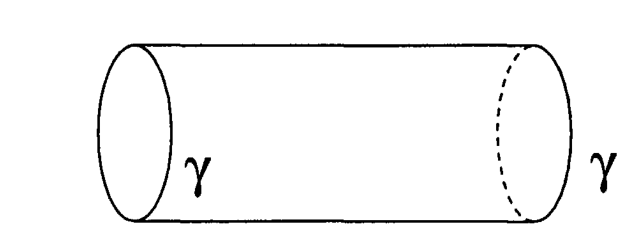
\includegraphics[width=0.42\textwidth]{figs/fig_p183_1.png}
  \caption{两端和乐均为 $\gamma$ 的柱面；右端的虚线表示远端的边界圈。（原文 Figure 1，p.183）}
  \label{fig:p183-1}
\end{figure}

% [Tutor Note: 这里的双重手续容易混淆：先固定边界上的和乐 $\gamma$ 得到扭曲扇区 $\mathcal{H}_\gamma$，再对残余的 $\mathbf{Z}_n$ 取不变子空间。$\mathbf{Z}_n$ 在 $\mathcal{H}_\gamma$ 上的作用来自绕空间圆的大规范变换；正因为 $\mathbf{Z}_n$ 阿贝尔，沿时间方向的扭曲 $\gamma'$ 与沿空间方向的 $\gamma$ 可以对易，$\gamma'$ 才能在 $\mathcal{H}_\gamma$ 上有良好定义并取迹。若群非阿贝尔，$\gamma'$ 一般不再把 $\mathcal{H}_\gamma$ 映到自身，必须按共轭类重组扇区——那是非阿贝尔轨形化的额外结构，本讲的论证不适用。]

如我们已经注意到的，$\mathbf{Z}_n$ 在每个扇区 $\mathcal{H}_\gamma$ 上仍有作用；设 $\gamma'\in\mathbf{Z}_n$ 决定一个算符 $\gamma':\mathcal{H}_\gamma\to\mathcal{H}_\gamma$。这个算符的迹可以作为一个环面上的配分函数 $Z_{\gamma'\gamma}$ 来计算：

\begin{figure}[htbp]
  \centering
  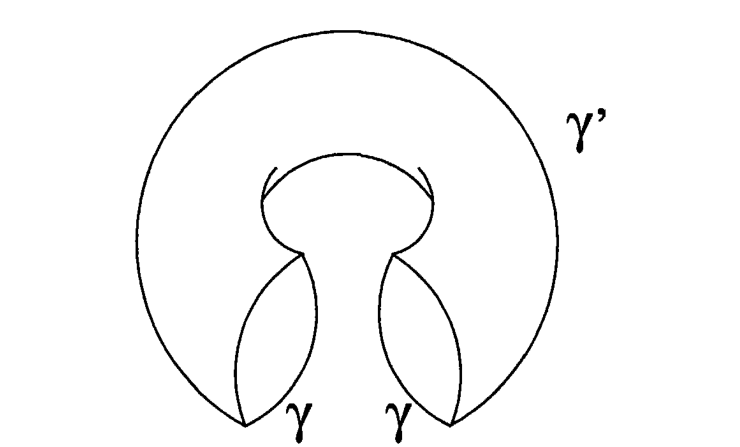
\includegraphics[width=0.46\textwidth]{figs/fig_p183_2.png}
  \caption{在环面上计算 $\mathrm{Tr}_{\mathcal{H}_\gamma}\gamma'q^{H}$：外侧大圈标以 $\gamma'$，底部两个小圈标以 $\gamma$，表示两个方向上分别作 $\gamma'$ 与 $\gamma$ 的扭曲。（原文 Figure 2，p.183）}
  \label{fig:p183-2}
\end{figure}

% ===== 原文 p.184 =====
它是用 $\gamma'$ 去扭曲柱面边界圈上丛的认同（identification）而构造的，即
\[
  Z_{\gamma'\gamma}=\mathrm{Tr}_{\mathcal{H}_\gamma}\,\gamma'\,q^{H}.
\]
更内蕴地说，在这个环面上，一个方向上有 $\gamma$ 的扭曲，另一个方向上有 $\gamma'$ 的扭曲，如图所示。

如果把各算符 $\gamma'$ 求和，结果便是 $n\pi$，其中 $\pi$ 是到 $\mathbf{Z}_n$ 不变子空间上的投影：
\[
  \frac{1}{n}\sum_{\gamma'}Z_{\gamma'\gamma}
  =\mathrm{Tr}_{\mathcal{H}_\gamma}\,\pi\,q^{H}
  =\mathrm{Tr}_{(\mathcal{H}_\gamma)^{\mathbf{Z}_n}}\,q^{H}.
\]
现在，$\mathbf{Z}_n$ 规范理论的配分函数可由下述方式得到：把亏格一的配分函数对所有方向上的一切可能扭曲求和，并（由于我马上要说明的理由）除以 $n$。这给出
\[
  \frac{1}{n}\sum_{\gamma,\gamma'}Z_{\gamma'\gamma}
  =\mathrm{Tr}_{\oplus_\gamma(\mathcal{H}_\gamma)^{\mathbf{Z}_n}}\,q^{H},
\]
由此我们断定，我们问题的 Hilbert 空间确实就是 $\mathcal{H}=\bigoplus_\gamma(\mathcal{H}_\gamma)^{\mathbf{Z}_n}$。

% [Tutor Note: $\sum_{\gamma'}\gamma'=n\pi$ 是有限群上的标准平均：在 $\mathbf{Z}_n$ 的正则表示中，非单位元素的特征标之和为零，故求和恰为 $|G|$ 倍到不变子空间的投影算符（等价地，$\frac1n\sum_{\gamma'}\gamma'$ 是投影）。随后出现的两个 $n$ 容易混淆：第一个 $1/n$ 来自对扭曲 $\gamma'$ 的平均，第二个 $1/n$（在 $\frac1n\sum_{\gamma,\gamma'}$ 中）来自除以规范群体积 $|G|=n$。二者数值相同而来源不同；漏掉任何一个都会使配分函数整体差一个 $n$ 的因子，从而把 Hilbert 空间的维数算错。]

或许我应当解释一下，为什么
\[
  Z=\frac{1}{n}\sum_{\gamma,\gamma'}Z_{\gamma'\gamma}
\]
才是 $\mathbf{Z}_n$ 规范理论合适的配分函数。在规范理论中作路径积分时，人们应当对联络求和并除以规范群的体积。当规范群是正维数的 Lie 群时，联络的空间是无穷维的。规范变换群同样是无穷维的，而要使“除以规范群的体积”这句话有意义，就需要 Faddeev–Popov 构造并引入鬼场。在目前的情形中，我们考虑的是规范群为 $\mathbf{Z}_n$ 的低能有效理论。$\Sigma$ 上仅有的联络就是取值于 $\mathbf{Z}_n$ 的平坦联络。所以对 $\gamma$ 与 $\gamma'$ 的求和就是关于联络的路径积分。$\Sigma$ 上仅有的规范变换是由 $\mathbf{Z}_n$ 的元素所作的常值变换；因此规范群的体积就是 $n$，即规范群元素的个数。于是“除以规范群的体积”就由除以 $n$ 来实现。

\subsection{从正 $r$ 到负 $r$ 的插值}
% 原文 §13.4.3

我们的经典分析可以总结如下：我们需要令 $D=dW=0$，并除以 $U(1)$。令 $D=0$ 并除以 $U(1)$ 这一步，就是数学上熟悉的辛约化（symplectic reduction）操作，其中 $D=0$ 定义了 $U(1)$ 作用的矩映射的一个水平集（$r$ 的选取指定了该水平）。这一过程还有另一种数学解释，即几何不变量理论（Geometric Invariant Theory，GIT）意义下的商：我们把群 $U(1)$ 复化为 $\mathbb{C}^{*}$，并考虑 $\mathbb{C}^{*}$ 以与前面相同的权在 $\mathbb{C}^{n+1}$ 上的作用（$A_i$ 的权为 $1$，$P$ 的权为 $-n$）。在这个具体例子中存在两种可能的 GIT 商（它们实际上拓扑不同）：当 $r>0$ 时，该商可以解释为丛 $\mathcal{O}_{\mathbf{P}^{n-1}}(-n)$ 的全空间（其中 $p$ 充当纤维坐标），而当 $r<0$ 时，该商是 $\mathbb{C}^{n}/\mathbf{Z}_n$。

% ===== 原文 p.185 =====
在两种情形下我们都还必须施加 $dW=0$：在 $r>0$ 的情形，$W=PF(A_1,\dots,A_n)$ 是一个非退化函数（在 Bott 引入的广义意义下），而 $\mathcal{O}_{\mathbf{P}^{n-1}}(-n)$ 中临界点的集合就是 $\mathbf{P}^{n-1}$ 中由方程 $F=0$ 定义的那个簇；在 $r<0$ 的情形，我们有一个齐次多项式 $F(A_1,\dots,A_n)$，它在 $\mathbb{C}^{n}/\mathbf{Z}_n$ 的原点处有高度退化的临界点。

我们拉氏量中的自然参数是 $t=-ir+\frac{\theta}{2\pi}$。正是由于可以取 $\theta\ne0$，我们才能从正 $r$ 插值到负 $r$，而不遇到经典几何中会碰到的那个奇点。

\begin{figure}[htbp]
  \centering
  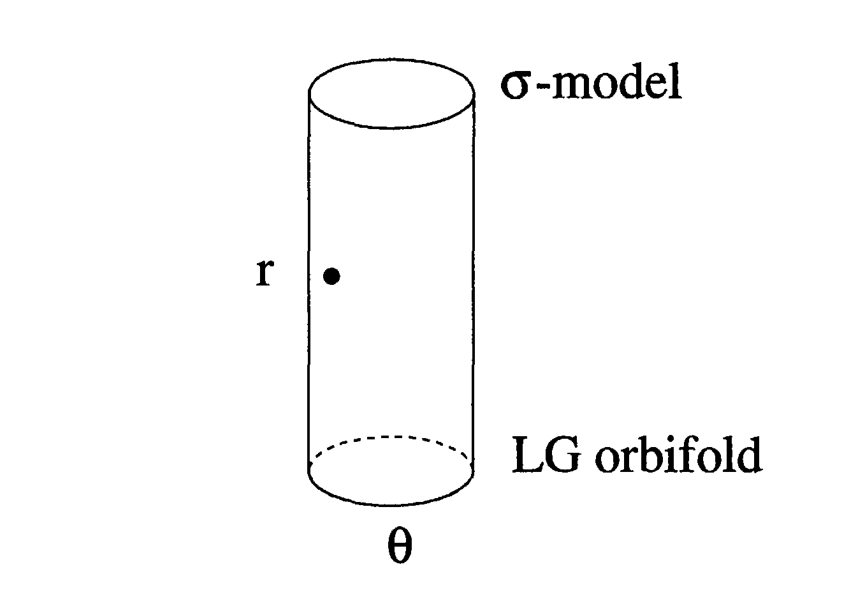
\includegraphics[width=0.40\textwidth]{figs/fig_p185_1.png}
  \caption{参数空间的柱面：竖直方向为 $r$，水平方向为 $\theta$，即复坐标 $t=-ir+\frac{\theta}{2\pi}$；上端 $r\gg0$ 处是 $\sigma$ 模型，下端 $r\ll0$ 处是 Landau–Ginzburg 轨形，柱面上的黑点标出 $r=0$ 处的奇点。（原文 Figure 3，p.185）}
  \label{fig:p185-1}
\end{figure}

经典地，在任意 $\theta$ 下 $r=0$ 处都有奇点，因而插值是不可能的。量子力学地，我们断言这个奇点将是孤立的，位于 $r=r_0$（对某个 $r_0$）且 $\theta=0$。（经典地奇点在 $r=0$；但量子力学地，它被一个我们即将讨论的单圈修正从 $r=0$ 移开了。）人们相信没有别的奇点；我们不会严格证明这一断言，而只解释物理学家相信它为真的一些理由。我们分析中较严格的部分，将是论证在这个位置确实存在奇点；较不严格的部分，则是论证这是唯一的奇点。

为作这一论证，我们再次把空间取为半径有限的圆 $S^{1}$。紧致性意味着情况与零空间维数中的普通量子力学颇为相似，所以我们先回顾一下质点普通量子力学中会发生什么。设粒子在流形 $X$ 上运动，势函数为 $V$。如果 $X$ 紧致，或者 $V$ 在 $X$ 的“两端”增长，那么我们可以变动 $X$ 与 $V$ 所依赖的参数，而不遇到量子力学基态的奇点。然而，若把参数变到某一点，使得 $V$ 在无穷远处不再增长，就会得到奇点。例如，若 $X=\mathbf{R}$，$V=\frac12 kx^{2}$（$x$ 为 $\mathbf{R}$ 上的线性函数），则只要 $k>0$，基态波函数就是 $k$ 的光滑函数，但在 $k=0$ 处会出现奇点。$k=0$ 的问题没有可归一化的基态波函数。

在我们的圆上问题中也会发生类似的事情。回忆我们的势的形式是
\[
  V=|P|^{2}|F|^{2}+|dF|^{2}
  +\frac{e^{2}}{2}\Bigl(\sum|A_i|^{2}-n|P|^{2}-r\Bigr)^{2}
  +|\sigma|^{2}\Bigl(\sum|A_i|^{2}+n^{2}|P|^{2}\Bigr).
\]

% [Tutor Note: 上式前两项印作 $|P|^{2}|F|^{2}+|dF|^{2}$，与 (13.5) 的 $|dW|^{2}=|F|^{2}+|p|^{2}|dF|^{2}$ 不符，正确写法应为 $|F|^{2}+|P|^{2}|dF|^{2}$，即 $|P|^{2}$ 应当乘在 $|dF|^{2}$ 上。三条判据：(i) (13.5) 只是对 $W=PF(A)$ 求导的直接结果；(ii) p.182 的论证“$p\ne0$ 时 $|dW|^{2}=0\Rightarrow F=dF=0$”恰恰要求 $|F|^{2}$ 的系数为 $1$ 而不是 $|p|^{2}$，否则 $p\to0$ 时该项自动消失，横截性条件就用不上了；(iii) 只有当 $|P|$ 大时 $A_i$ 才获得 $|P|^{2}|dF|^{2}$ 型的大质量，这与 p.186 上“$A$、$P$ 很小时其质量量级为 $|\sigma|^{2}$”的讨论一致。故这是原书的排版笔误，译文按原文照录，并在正文外指出。]

对一般的 $r$，这个理论具有势在无穷远处增长的性质。这保证了理论有离散谱，且其基态波函数随参数光滑变化。然而在 $r=0$ 时我们看到，只要 $A_i$ 与 $P$ 趋于零，就可以在 $\sigma$ 方向走到无穷远而不付出能量代价。这提示

% ===== 原文 p.186 =====
在 $r=0$ 时可能存在连续谱，以及基态波函数的奇点。

为了更细致地研究这个问题，我们需要理解理论在危险区域（即 $\sigma$ 很大而其他场很小）中的行为。当 $A$ 与 $P$ 非常接近零、而 $\sigma$ 很大时，$A$ 与 $P$ 有很大的质量（量级为 $|\sigma|^{2}$），可以被积掉，留下一个纯规范理论，其有效玻色势在经典层面只是一个常数
\begin{equation}
  \tag{13.6}
  \label{eq:13-6}
  V_{\mathrm{eff}}=\frac{e^{2}}{2}r^{2}.
\end{equation}
如果这就是正确答案，那么能量小于 $e^{2}r^{2}/2$ 的量子态在 $\sigma$ 很大的区域中会指数衰减。若如此，这个区域只可能在 $r=0$ 时对零能的超对称基态构成危险——并导致这种态的波函数出现奇点。

为了更好理解这一情形，我们必须在量子层面作类似的论证。为此考虑 $\sigma$ 所属的那个超场，即写出
\[
  \Sigma=\sigma+\theta\lambda+\theta\bar\theta(F+iD).
\]
超对称规范理论的作用量为
\begin{equation}
  \tag{13.7}
  \label{eq:13-7}
  \frac{1}{2e^{2}}\int d^{4}\theta\,\bar\Sigma\Sigma
  +\Bigl(\int d\bar\theta^{+}\,d\theta^{-}\,t\Sigma+\text{c.c.}\Bigr).
\end{equation}
如果在有效拉氏量 (13.7) 中完成 $\theta$ 积分，我们得到
\[
  \frac{1}{e^{2}}\int d^{2}x\left(\frac{F^{2}}{2}+|d\sigma|^{2}+\bar\lambda\not{\partial}\lambda\right)
  +\int d^{2}x\left(\frac{e^{2}r^{2}}{2}\right)
  +i\theta\int_{\Sigma}\frac{F}{2\pi},
\]
其中既包含一个曲率项（乘以一个“$\theta$ 角”），也包含前面讨论过的玻色势。

% [Tutor Note: 注意 $\theta$ 积分前后系数的变化：作用量 (13.7) 中写的是 $\frac{1}{2e^{2}}\int d^{4}\theta\,\bar\Sigma\Sigma$，而积分后动能项前变成 $\frac{1}{e^{2}}$。具体数值因子取决于 $\theta$ 测度与 $\bar\Sigma\Sigma$ 展开的约定，不宜死记，可靠的核对办法是：只保留 $D$ 与 FI 项 $-rD$（即令 $A=P=0$），消去 $D$ 后必须回到 (13.6) 的 $\frac{e^{2}}{2}r^{2}$，也就是 p.185 上 $\frac{e^{2}}{2}\bigl(\sum|A_i|^{2}-n|P|^{2}-r\bigr)^{2}$ 在 $A=P=0$ 处的值。若整体因子记错，这里就会差一个 $2$ 或一个 $e^{2}$。另需分清两个同名符号：此式的 $F$ 是 $\Sigma$ 的辅助场，与超势 $W$ 的 $F$ 项（p.181 起一直记作 $F(A_i)$ 的那个多项式）不是一回事；而 $\bar\lambda\not{\partial}\lambda$ 中的 $\not{\partial}$ 是二维的 $\gamma^{a}\partial_{a}$。]

幸运的是，我们知道二维 $U(1)$ 规范理论中能量对 $\theta$ 的依赖；正如第 5 讲 §5.5 所计算的，它是
\[
  \frac{e^{2}}{2}\min_{n\in\mathbf{Z}}\left(n-\frac{\theta}{2\pi}\right)^{2}.
\]
于是当 $\sigma\to\infty$ 时，我们有 $V(\sigma)\sim\min_{n}\frac{e^{2}}{2}|\tilde t|^{2}$，其中 $\tilde t=-ir+\frac{\theta}{2\pi}+n$，$n\in\mathbf{Z}$。换言之，虽然 $\sigma$ 很大时的经典能量是 $e^{2}r^{2}/2$，但量子力学地 $r^{2}$ 被 $|\tilde t|^{2}$ 取代。因此，经典地奇点在 $r=0$ 而 $\theta$ 是不可见的；量子力学地，只有当 $\theta$ 为零时才出现奇点。对 $\tilde t$ 的任何其他取值，$\sigma\to\infty$ 时都有正能量，这个区域对超对称基态并不危险。

% [Tutor Note: 二维 $U(1)$ 规范理论中 $\int_{\Sigma}F/2\pi\in\mathbf{Z}$（$F$ 的积分给出第一 Chern 数），故 $\theta$ 项以 $2\pi$ 为周期；把 $\theta$ 并入 $t$ 之后，不同拓扑扇区的真空能就是 $\frac{e^{2}}{2}\bigl(n-\frac{\theta}{2\pi}\bigr)^{2}$，取最小值即“挑出最接近 $\theta/2\pi$ 的那个整数 $n$”。这解释了为何 $\tilde t=-ir+\frac{\theta}{2\pi}+n$ 中的 $n$ 可以自由平移：它标记大规范变换下的不同拓扑扇区，物理上彼此等价。作者随后把 $|\tilde t|^{2}$ 读作“到最近奇点的距离平方”，这与 $V\sim|\tilde t|^{2}$ 在 $\sigma\to\infty$ 时成立完全一致；也正因为要取 $\min$，$\theta\to\theta+2\pi$ 的周期性才是显然的。]

实际上还有一个相关的量子效应：一个单圈修正给出 $r$ 的有限重整化，并把奇点的位置从 $t=0$ 移到 $\tilde t=-ir_0$（对某个常数 $r_0$）。这个修正对于与经典几何的某些预言作比较是重要的，但对于我们今天要讲的内容并不重要。

\subsection{另一个例子：flop}
% 原文 §13.5

作为第二个例子，我们考虑规范群为 $G=U(1)$、手征场 $A_1,A_2$ 的电荷为 $1$、手征场 $B_1,B_2$ 的电荷为 $-1$、没有超势、也没有 “$P$” 的模型。拉氏量取如下形式

% ===== 原文 p.187 =====
\[
  \int d^{2}x\,d^{4}\theta\left(\frac{1}{2e^{2}}\bar\Sigma\Sigma+\sum\bigl(|A_i|^{2}+|B_i|^{2}\bigr)\right)
  +\Bigl(t\int d\bar\theta^{+}\,d\theta^{-}\,\Sigma+\text{c.c.}\Bigr).
\]
$D$ 项为
\[
  D=\sum\bigl(|A_i|^{2}-|B_i|^{2}\bigr)-r,
\]
而玻色势还含有一项
\[
  |\sigma|^{2}\sum\bigl(|A_i|^{2}+|B_i|^{2}\bigr).
\]

如以前一样，我们必须令 $D=0$ 并除以 $U(1)$。当 $r>0$ 时这给出 $\mathbf{P}^{1}_{A}$ 上丛 $\mathcal{O}(-1)\oplus\mathcal{O}(-1)$ 的全空间；而当 $r<0$ 时这给出 $\mathbf{P}^{1}_{B}$ 上丛 $\mathcal{O}(-1)\oplus\mathcal{O}(-1)$ 的全空间。这里 $\mathbf{P}^{1}_{A}$ 是 $\mathbf{P}^{1}$ 的一份拷贝，由要求 $A_1,A_2$ 不全为零、并把配对 $(A_1,A_2)$ 除以 $\mathbb{C}^{*}$ 而得到。类似地，$\mathbf{P}^{1}_{B}$ 是把 $(B_1,B_2)$ 投影化所得的 $\mathbf{P}^{1}$ 的一份拷贝。

从 $\mathbf{P}^{1}_{A}$ 上的丛到 $\mathbf{P}^{1}_{B}$ 上的丛的这一变换，是称为“flop”的双有理变换的一个简单模型。与前一个例子一样，奇点只在 $r=\theta=0$ 时出现，而人们可以在两个模型之间插值。这与经典几何形成对照：在经典几何中，从商 $\mathbb{C}^{4}/\mathbb{C}^{*}$ 的一个模型走到另一个模型，必须经过一个奇点。

\begin{figure}[htbp]
  \centering
  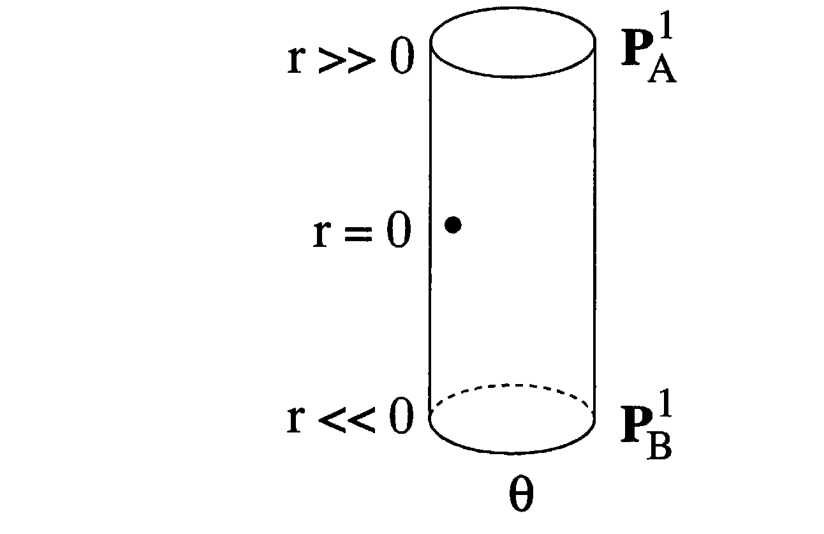
\includegraphics[width=0.40\textwidth]{figs/fig_p187_1.png}
  \caption{与 Figure 3 同构的参数柱面：$r\gg0$ 处靶空间为 $\mathbf{P}^{1}_{A}$ 上的 $\mathcal{O}(-1)\oplus\mathcal{O}(-1)$，$r\ll0$ 处为 $\mathbf{P}^{1}_{B}$ 上的同一丛，黑点标出 $r=0$ 处的奇点，水平方向为 $\theta$。（原文 Figure 4，p.187）}
  \label{fig:p187-1}
\end{figure}

更一般地，考虑两个双有理等价的 Calabi–Yau 流形 $X$ 与 $X'$，其等价方式使得它们的丰富锥（ample cone）彼此相接。

\begin{figure}[htbp]
  \centering
  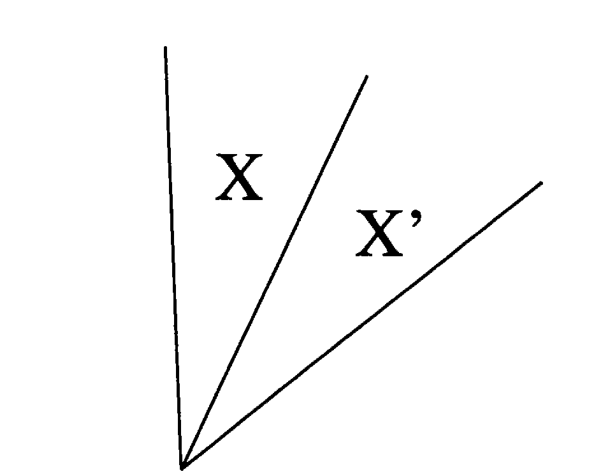
\includegraphics[width=0.36\textwidth]{figs/fig_p187_2.png}
  \caption{两个双有理等价的 Calabi–Yau 流形 $X$ 与 $X'$ 的 Kähler 锥沿一条公共的壁相接，图中以三条自原点出发的射线表示锥的边界。（原文 Figure 5，p.187）}
  \label{fig:p187-2}
\end{figure}

为简单起见设 $h^{2,0}=0$，并注意双有理变换不会改变 $h^{p,0}$ 的值。经典地，要从 $X$ 走到 $X'$，必须经过 Kähler 锥壁上的一个奇点。这个奇点与我们在“flop”例子中于 $r=0$ 处刚发现的奇点颇为相似。在量子场论中，人们可以取 $\theta\ne0$ 绕过这个奇点；于是只要变动共形场论的参数，就能从 $X$ 光滑地延拓到 $X'$。

% [Tutor Note: 这个“flop”例子其实就是 conifold（锥形奇点）：$\mathbb{C}^{4}$ 在 $\mathbb{C}^{*}$ 的权 $(1,1,-1,-1)$ 作用下的两个 GIT 商，正是 conifold 的两个“小解消” $\mathcal{O}(-1)\oplus\mathcal{O}(-1)\to\mathbf{P}^{1}$，而 flop 就是连接二者的双有理变换。两侧都是 $h^{1,1}=1$、$h^{2,1}=0$，且 $h^{p,0}$ 在 flop 下不变，这与正文“双有理变换不改变 $h^{p,0}$”相符（一般 flop 会使 $h^{1,1}$ 改变 $\pm1$、$h^{2,1}$ 反向改变而 Euler 数不变；本例中两个小解消同构，故 Hodge 数完全不变）。经典几何必须穿过 conifold 奇点，量子场论则借 $\theta\ne0$ 绕过——这是“量子几何把经典上必须退化的模空间光滑地连起来”的典型例子。另外，“$h^{2,0}=0$”对 Calabi–Yau 三维复流形（threefold）本已自动成立，作者写下它是为了排除由 $h^{2,0}$ 型周期（$B$ 场）带来的额外参数，使复化 Kähler 模空间成为唯一相关的模空间。]

% 原文 pp.188–194（印刷 pp.1306–1312）
% 承接第 13 讲第 2 部分：本文件自 §13.6 起，故不写 \section

% ===== 原文 p.188 =====

例如，我们可以这样构造一对 $h^{1,1}=2$ 的 Calabi--Yau 流形：从规范群 $G=U(1)\times U(1)$ 以及形如 $W=PF(A_i)$ 的超势出发。
只要设置得当，其中一个 $U(1)$ 就把我们带入射影簇（projective variety）$X$ 与 $X'$ 的世界；而通过改变另一个 $U(1)$ 的矩映射（moment map），我们便可以在 $X$ 与 $X'$ 之间做出一个「flop」，它与上面关于四个手征超场 $A_i$、$B_j$ 的讨论十分相似。

% [Tutor Note: 「flop」与 Fayet--Iliopoulos 参数的关系值得说清。线性 $\sigma$ 模型中 $U(1)$ 的 FI 参数 $r$ 与 $\theta$ 角组合成复参数 $t$；把 (13.8) 的临界点方程与 p.190 的分量形式 $0=-ir+\frac{\theta}{2\pi}-\frac{in}{2\pi}\ln(\sigma/\mu)$ 对照，即可定出本文的约定 $t=\frac{\theta}{2\pi}-ir$（实部是 $\theta$ 角、虚部是 FI 参数，二者地位并不对称）。$r$ 穿过 $0$ 时，$D$ 项条件所定义的商空间从一个相「翻转」到另一个相，这正是 flop 的线性 $\sigma$ 模型实现。这一约定还有一个可检验的推论：p.191 末尾的奇点判据 $t-\frac{i}{2\pi}\sum_i q_i\ln|q_i|=0$ 是纯虚的，故奇点只落在 $\theta\equiv0\pmod{2\pi}$、$r=-\frac{1}{2\pi}\sum_i q_i\ln|q_i|$ 处，而不会在 $\theta$ 方向移动；若把 $t$ 的实虚部记反，就会得出「奇点随 $\theta$ 平移」的错误结论。另：原文此句作 ``the four chiral superfields fields $A_i$ and $B_j$''，``fields'' 重出，应属笔误，译文按「四个手征超场」处理。]

\subsection{$c_1\ne0$ 的情形}
% 原文 §13.6：Cases in which $c_1\ne0$

现在我们要考虑 $R$ 对称性反常的线性 $\sigma$ 模型（linear sigma model），因此预期存在非平凡的重整化群流。

\subsubsection{负 $\beta$ 函数}
% 原文 §13.6.1：Negative $\beta$-function

我们从负 $\beta$ 函数的情形开始；对非线性 $\sigma$ 模型而言，这对应于满足 $c_1(TX)>0$ 的目标空间 $X$。
这类例子可以完全照旧构造：让 $U(1)$ 作用在 $n+1$ 个场 $A_i,P$ 上，但这一次赋给 $P$ 荷 $-k$，并取超势 $W=P\cdot F$，其中 $F$ 是 $k$ 次齐次多项式。
该 $\sigma$ 模型的 $\beta$ 函数在 $k<n$、$k=n$、$k>n$ 时依次为负、零、正。

% [Tutor Note: 「负 $\beta$ 函数 $\Leftrightarrow c_1(TX)>0$」用的是 $\beta=\mu\,dg/d\mu$ 的约定，即负 $\beta$ 函数就是渐近自由；其几何判据是目标空间的 Ricci 形式正定，等价于 $c_1(TX)>0$（Fano）。若换成 $\beta=-\mu\,dg/d\mu$ 的相反约定（部分文献如此），则整段关于 $k\lessgtr n$ 的结论要全部反号，这是读文献时最易翻车之处。另请注意本段有两处结论都以 $k\ne n$ 为前提，而 $k=n$（Calabi--Yau）恰是 $c_1=0$、$\beta=0$ 的临界情形，此时既无红外不动点也无紫外不动点，故被排除在讨论之外。]

对 $k\ne n$，尽管经典地看 $r=0$ 处仍有奇点，量子理论在 $t$ 柱面（$t$-cylinder）上却没有奇点。
（这一点通过分析大 $\sigma$ 处的行为来证明，我们马上就会做。）
对 $k\ne n$，柱面上存在非平凡的重整化群流。
该流是全纯的、无奇点的，因此它是柱面上「向下」或「向上」的匀速流，方向取决于 $n-k$ 的符号。

\begin{figure}[htbp]
  \centering
  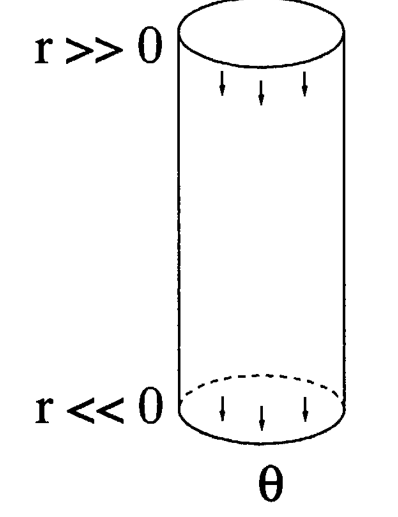
\includegraphics[width=0.30\textwidth]{figs/fig_p188_1.png}
  \caption{$t$ 柱面：竖直方向为 $r$，绕柱的圆周方向为 $\theta$ 角。顶端标注 $r\gg0$（$\sigma$ 模型端），底端标注 $r\ll0$（Landau--Ginzburg 端），柱面上的箭头示意重整化群流的方向。（原文 Figure 6，p.188）}
  \label{fig:p188-1}
\end{figure}

当我们重复先前的分析时，会发现来自四维 $R$ 对称性的那个 $R$ 对称性是反常的，而来自缺失方向转动的那个 $R$ 对称性则无反常。

经典分析同样可以重复：对 $r\gg0$，我们得到由 $\mathbf{P}^{n-1}$ 中的 $\{F=0\}$ 描述的经典真空空间，并预期该超曲面上的非线性 $\sigma$ 模型是我们理论的良好近似。
当 $k<n$ 时，这个超曲面具有正的第一 Chern 类，因此从非线性 $\sigma$ 模型出发，我们预期得到一个定义良好的量子场论。
另一方面，由于 $k<n$，该 $\sigma$ 模型在红外是不稳定的。
红外流会把我们带离 $\sigma$ 模型，趋向我们在 $r\to-\infty$ 极限处将找到的理论。
注意该 $\sigma$ 模型的目标空间是 $(n-2)$ 维的，因此在 $k<n$ 时，紫外极限下的有效中心荷为 $\widehat{c}=n-2$。

另一方面，若 $r\ll0$，则经典真空空间上 $P\ne0$ 而 $A_i=\sigma=0$。
给 $P$ 一个非零期望值把 $U(1)$ 破缺为 $\mathbf{Z}_k$，并且（在

% ===== 原文 p.189 =====

$r\to-\infty$ 极限下）我们得到一个 Landau--Ginzburg 轨形（orbifold），其有效相互作用为
\[
W_{\rm eff}(A_i)=F(A_i).
\]
该模型的中心荷为
\[
\widehat{c}=n\Bigl(1-\frac{2}{k}\Bigr).
\]
当 $k<n$ 时它小于 $n-2$。
我们稍后将论证：对 $k<n$，Landau--Ginzburg 理论正是从 $\sigma$ 模型出发的重整化群流的红外极限；而它的中心荷比 $\sigma$ 模型的小这一事实，恰好说明了 Zamolodchikov 的一个一般定理——该定理断言中心荷沿重整化群流总是减小：
\[
c_{\rm IR}\le c_{\rm UV}.
\]

% [Tutor Note: 作者在 $c$ 与 $\widehat{c}$ 之间来回切换，必须按 $c=3\widehat{c}$ 换算（二维 $\mathcal N=2$ 超共形代数的标准归一化：$W=\Phi^k$ 的 Landau--Ginzburg 模型有 $\widehat{c}=1-2/k$，对应 $A_{k-1}$ 极小模型的 $c=3(k-2)/k$）。因此 $c_{\rm IR}\le c_{\rm UV}$ 与 $\widehat{c}_{\rm IR}\le\widehat{c}_{\rm UV}$ 等价，本页的数值比较（如 $\widehat{c}=n(1-2/k)<n-2$）不受影响；但切勿把某页的 $\widehat{c}$ 与另一页的 $c$ 直接相减，否则会差一个因子 3。另需注意：$\widehat{c}=n(1-2/k)$ 是 $n$ 个手征超场、超势次数为 $k$ 的 LG 轨形的值，其中的 $P$ 场因获得质量而不计入；轨形化（orbifold）本身不改变中心荷。]

该定理背后的直观是：中心荷衡量理论中自由度的总数。
随着向红外流动，有质量的自由度被「积掉」（integrated out），不再对中心荷有贡献，因此中心荷只可能减小。

我们将看到，对 $k<n$，Landau--Ginzburg 模型只是红外流可能达到的结果之一。
事实上在 $r=-\infty$ 处还有 $n-k$ 个另外的真空态，它们有质量间隙（mass gap），经典上看不见，需要用单圈计算才能得到。
由于有质量，它们的 $\widehat{c}=0$，当然小于 $n-2$。

\subsubsection{$\mathbf{CP}^{n-1}$ 模型}
% 原文 §13.6.2：The $\mathbf{CP}^{n-1}$ model

我们所考虑的情形的一个极端例子是 $k=0$，即没有 $P$ 场、也没有超势的情形。
这是一个带 $n$ 个自由带电超场 $A_1,\dots,A_n$（荷全为 $1$）的 $U(1)$ 规范理论。
$D$ 项取如下形式
\[
D=\sum_i|A_i|^2-r.
\]
令它为零再除以 $U(1)$，我们便得到（对 $r\gg0$）先前某一讲中研究过的超对称 $\mathbf{CP}^{n-1}$ 模型。
在回到一般情形之前，详细重审这个例子将极有启发。

乍看之下，这个 $\mathbf{CP}^{n-1}$ 模型在 $r\to-\infty$ 极限下似乎根本没有超对称真空，因为矩映射是严格正的。
然而，在这个极限下根本不存在超对称真空是不可能的。
超对称指标 $\operatorname{Tr}(-1)^F$ 提供了阻碍。（我在去年秋季的讲座中讨论过这个指标及其推广——椭圆亏格。）
对大的正 $r$ 计算，这个指标与 $\mathbf{CP}^{n-1}$ 的 Euler 特征数相等，即为 $n$。
超对称指标在 $r$ 的形变下必须不变，因此即使 $r$ 很大且为负，也必须存在 $n$ 个超对称真空。
我们总得在某处找到它们！

要看清究竟发生了什么，我们必须更仔细地考察量子力学。
对 $r\to-\infty$ 极限的经典处理在场空间的任何紧区域中都成立，因此，如果对任意负的 $r$ 存在经典上看不见的量子力学真空，那么当 $r\to-\infty$ 时它们必须以「跑到场空间无穷远」的方式从经典视野中消失。
所以我们必须再次考察大 $\sigma$ 处的量子力学行为。
对我们的 $\mathbf{CP}^{n-1}$ 模型，玻色子势取如下形式
\[
V=\frac{e^2}{2}D^2+|\sigma|^2\sum_i|A_i|^2.
\]

% ===== 原文 p.190 =====

该理论在 $r\ll0$ 时是弱耦合的。

若 $|\sigma|\to\infty$ 会怎样？
与先前一样，此时场 $A_i$ 将获得质量，可以被积掉，从而得到一个阿贝尔规范理论作为有效理论，其拉氏量为
\[
\mathcal{L}_{\rm eff}=\int d^2x\,d^4\theta\,\frac{1}{2e^2}\overline{\Sigma}\Sigma
+\Bigl(\int d^2x\,d\bar\theta^+\,d\theta^-\,\widetilde{\mathcal{W}}_{\rm eff}(\Sigma)+{\rm c.c.}\Bigr).
\]
有效扭曲超势（twisted superpotential）依赖于重整化质量标度 $\mu$，而我们断言它取如下新颖的（破坏 $R$ 对称性的）形式
\begin{equation}
  \tag{13.8}
  \label{eq:13-8}
  \widetilde{\mathcal{W}}_{\rm eff}(\Sigma)=t\Sigma+\frac{in}{2\pi}\bigl(\Sigma-\Sigma\ln(\Sigma/\mu)\bigr),
\end{equation}
我们将通过下面的单圈计算来验证它。
注意，在 (13.8) 中改变对数的选取，可以由把 $t$ 的值改变一个整数来补偿；这样的改变对物理没有影响。
当然，为了使 $\widetilde{\mathcal{W}}_{\rm eff}$ 中的对数有定义，我们必须让 $\Sigma$ 远离零，这与我们假设 $\sigma$ 很大是一致的。

% [Tutor Note: 「把 $t$ 改变一个整数」可以显式验证：绕一圈 $\ln\Sigma\to\ln\Sigma+2\pi i$ 使 $\widetilde{\mathcal{W}}_{\rm eff}\to\widetilde{\mathcal{W}}_{\rm eff}+\frac{in}{2\pi}(-\Sigma\cdot2\pi i)=\widetilde{\mathcal{W}}_{\rm eff}+n\Sigma$，即 $t\to t+n$，而 $n$ 是带电场的个数、必为整数，等价于 $\theta\to\theta+2\pi n$。这里应当警惕两点：(i) 移动的是 $t$ 的实部（$\theta$），不是虚部（$r$），因为 $\frac{in}{2\pi}\Sigma\cdot2\pi i$ 的符号由 $+i$ 与 $+2\pi i$ 相乘决定，极易写反；(ii) 若超势中写成 $\Sigma\ln\Sigma$ 而非 $\Sigma\ln(\Sigma/\mu)$，则 $t$ 的平移还会带上 $\ln\mu$，重整化标度的意义就丢失了——这正是作者保留 $\mu$ 的原因。]

有了扭曲超势中的这一新项，$\widetilde{\mathcal{W}}_{\rm eff}$ 的临界点方程为
\[
0=t-\frac{in}{2\pi}\ln(\Sigma/\mu),
\]
或者写成分量形式，
\[
0=-ir+\frac{\theta}{2\pi}-\frac{in}{2\pi}\ln(\sigma/\mu)\pmod 1.
\]
它有 $n$ 个解
\begin{equation}
  \tag{13.9}
  \label{eq:13-9}
  \sigma=\mu\exp\Bigl(-\frac{2\pi r}{n}-\frac{i\theta}{n}+\frac{2\pi ik}{n}\Bigr),\qquad
  k=0,\dots,n-1,
\end{equation}
对应于 $r\to-\infty$ 极限下 $n$ 个不同的真空。
$n$ 当然正是预期的数目，即 $\mathbf{CP}^{n-1}$ 的 Euler 特征数。
注意当 $r\to-\infty$ 时 $|\sigma|$ 确实很大，因此推导这些真空时所作的假设成立。
这 $n$ 个真空在 $r\to-\infty$ 时跑向场空间的无穷远，而它们的存在又依赖于单圈量子修正，这两点合起来解释了为什么经典上看不见它们。

对数的另一个非常重要的推论是：当 $\sigma\to\infty$ 时，量子理论中的能量按 $|\ln\sigma|^2$ 增长。
因此特别地，低能态被限制在场空间的一个有界区域内，从而对柱面上 $t$ 的任何取值，真空行为都不会出现奇点。
我们将会看到，$n\ne k$ 的模型都有这样的对数，因此它们在整个 $t$ 柱面上都是非奇异的。

\subsubsection{单圈计算}
% 原文 §13.6.3：The 1-loop calculation

要理解有效扭曲超势中 $\frac{in}{2\pi}\bigl(\Sigma-\Sigma\ln(\Sigma/\mu)\bigr)$ 这一项的起源，注意它的存在等价于有效拉氏量含有一项
\[
\int d^2x\,r_{\rm eff}D,
\]
其中
\[
r_{\rm eff}=r+\frac{n}{2\pi}\ln(|\sigma|/\mu).
\]

% ===== 原文 p.191 =====

在这个理论中，$D=\sum_i\overline{A}_iA_i-r$。
经典地，对大 $\sigma$ 有 $A_i=0=\overline{A}_iA_i$，但量子地，$\overline{A}_iA_i$ 在大 $\sigma$ 处有期望值；这个期望值在有效的经典描述中可以解释为 $-r$ 的一个平移。
因此我们需要借助单圈图来计算 $\overline{A}A$ 的期望值

\begin{figure}[htbp]
  \centering
  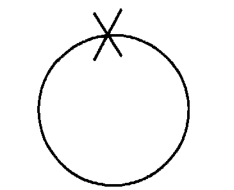
\includegraphics[width=0.16\textwidth]{figs/fig_p191_1.png}
  \caption{计算 $\langle\overline{A}_iA_i\rangle$ 的单圈图：一个闭合的玻色子圈，顶部的叉号代表 $\overline{A}A$ 算符插入（外线）。该图的贡献即下式的动量积分。（原文 Figure 7，p.191）}
  \label{fig:p191-1}
\end{figure}

它对 $\langle\overline{A}_iA_i\rangle$ 的贡献为
\[
\int\frac{d^2k}{(2\pi)^2}\frac{1}{k^2+m_A^2}
=\int\frac{d^2k}{(2\pi)^2}\frac{1}{k^2+|\sigma|^2},
\]
其中质量 $m_A$ 来自势 $V$ 中的 $|\sigma|^2|A|^2$ 项。
把这个发散积分截断，我们得到
\[
\int^\Lambda\frac{d^2k}{(2\pi)^2}\frac{1}{k^2+|\sigma|^2}
=-\frac{1}{2\pi}\ln\frac{|\sigma|}{\mu}+\frac{1}{2\pi}\ln\frac{\Lambda}{\mu}.
\]

% [Tutor Note: 这个二维圈积分最容易错在因子 2 上：$\int^\Lambda\frac{d^2k}{(2\pi)^2}\frac{1}{k^2+m^2}=\frac{1}{4\pi}\ln\frac{\Lambda^2+m^2}{m^2}\simeq\frac{1}{2\pi}\ln\frac{\Lambda}{m}$。也就是说 $\frac{1}{4\pi}$ 来自二维相空间，而 $\ln\Lambda^2=2\ln\Lambda$ 又补上一个 2，最终系数是 $\frac{1}{2\pi}$ 而不是 $\frac{1}{4\pi}$；若用 Pauli--Villars 或维数正规化而忘记这个 2，后面 (13.8) 中的 $\frac{in}{2\pi}$ 就会变成 $\frac{in}{4\pi}$，与 $\theta$ 的 $2\pi$ 周期性冲突。]

这里 $\mu$ 是重整化过程中引入的质量，而在本例中，重整化不过就是把 $\ln\frac{\Lambda}{\mu}$ 项丢掉（它与 $\sigma$ 无关，因而可以通过 $r$ 的重整化被抵消）。
重整化之后的这个公式给出 $-r$ 的一个依赖于 $\sigma$ 的平移，从而解释了所断言的 $r_{\rm eff}$ 的公式。
顺便说一句，这个公式没有更高圈的修正。
这可以用全纯性来证明，也可以这样看：在这个超可重整（superrenormalizable）理论中，更高圈的图会含有 $\sigma$ 的负幂次，在大 $\sigma$ 时趋于零。

现在对带荷 $q_i$ 的手征超场 $B_i$ 的一般情形重复上述计算。
（这里的 $B_i$ 应包括全部手征超场；若 $\sigma$ 模型讨论中的 $P$ 场存在，也包括它。）
$D$ 项为 $\sum_i q_i|B_i|^2$，其在大 $\sigma$ 处的期望值给出单圈修正
\[
\sum_i q_i\int^\Lambda\frac{d^2k}{(2\pi)^2}\frac{1}{k^2+q_i^2|\sigma|^2}
=-\frac{1}{2\pi}\sum_i q_i\ln|q_i|
-\frac{1}{2\pi}\Bigl(\sum_i q_i\Bigr)\ln\frac{|\sigma|}{\mu},
\]
由此得到有效扭曲超势
\[
\widetilde{\mathcal{W}}_{\rm eff}(\Sigma)
=\Bigl(t-\frac{i}{2\pi}\sum_i q_i\ln|q_i|\Bigr)\Sigma
+\frac{i\sum_i q_i}{2\pi}\bigl(\Sigma-\Sigma\ln(\Sigma/\mu)\bigr).
\]

% [Tutor Note: 与上面 p.191 单个场的截断结果相比，这个求和式里少了一项 $+\frac{1}{2\pi}\bigl(\sum_i q_i\bigr)\ln\frac{\Lambda}{\mu}$：逐项代入 $m=|q_i||\sigma|$ 即可看出，$\ln\Lambda$ 的系数恰是 $\sum_i q_i$，因此它是 $\sigma$ 无关的常数，被 $t$ 的重整化吸收（$t\to t+\frac{i}{2\pi}\sum_i q_i\ln\frac{\Lambda}{\mu}$）。当 $\sum_i q_i=0$（Calabi--Yau 情形）时这一项自动为零，这正是 p.192 脚注（原文脚注 2）所说的「无需重整化」；不要把它当成笔误去补进全纯的 $\widetilde{\mathcal{W}}_{\rm eff}$。另注意 $\ln|q_i|$ 的绝对值不可省：$P$ 场的荷 $-k$ 为负，$\ln q_i$ 无定义。]

在 Calabi--Yau 情形，$\sum_i q_i=0$，对数的系数为零。
于是 $\widetilde{\mathcal{W}}_{\rm eff}$ 对 $\Sigma$ 是线性的，因此它对势能的贡献与 $\sigma$ 无关。
这样一来，只要 $t$ 取正确的值，$\sigma$ 就可以不付出任何能量代价地跑向无穷远。
在 $t$ 取这个值时就会出现奇点。
正确的值就是使扭曲手征超势中 $\Sigma$ 的系数为零的那个值；条件不是人们经典上会预期的 $\operatorname{Im}(t)=0$，甚至也不是 $t=0$，而是 $t-\frac{i}{2\pi}\sum_i q_i\ln|q_i|=0$。
这就是我们在讨论 Calabi--Yau

% ===== 原文 p.192 =====

情形时提到的奇点位置的平移。\footnote{原文脚注 2：当 $\sum_i q_i=0$ 时，单圈修正中的 $\ln\Lambda$ 项自行相消，无需任何重整化。因此，奇点位置平移的数值不会受任何可能任意的重整化程序影响。}
为了把当前的讨论与例如 Calabi--Yau 流形上有理曲线的计数相比较，了解这一平移是很重要的。
当 $\sum_i q_i\ne0$ 时，对数使得 $\sigma$ 不能跑向无穷远，从而（如我们已经断言的）阻止了 $t$ 柱面上出现奇点。

另一方面，若 $\sum q_i\ne0$，则（如同 $\mathbf{CP}^{n-1}$ 模型那样）还有 $\bigl|\sum q_i\bigr|$ 个额外的真空，其 $\sigma$ 值为
\begin{equation}
  \tag{13.10}
  \label{eq:13-10}
  \sigma=\mu\exp\Bigl(
  -\frac{2\pi r}{\sum q_i}
  -\frac{i\theta}{\sum q_i}
  -\frac{\sum q_i\ln q_i}{\sum q_i}
  +\frac{2\pi ik}{\sum q_i}\Bigr),
\end{equation}
然而，对这些真空的预言只在它们出现于大 $\sigma$ 处时才有效。
因此，只有当 $\sum_i q_i>0$ 时它们在 $r\to-\infty$ 才可信，或者只有当 $\sum_i q_i<0$ 时它们在 $r\to+\infty$ 才可信。

% [Tutor Note: (13.10) 的第三项在原文中印作 $\frac{\sum q_i\ln q_i}{\sum q_i}$，但按 p.191 的推导（那里明确是 $\ln|q_i|$）与 (13.9) 的同类结构，应为 $\frac{\sum_i q_i\ln|q_i|}{\sum_i q_i}$：$q_i$ 中至少有一个（$P$ 场的 $-k$，$k>0$）取负值，$\ln q_i$ 本身没有定义，故绝对值不可省。代入法可自检：由 $0=t-\frac{i}{2\pi}\sum q_i\ln|q_i|-\frac{i\sum q_i}{2\pi}\ln(\sigma/\mu)$ 解出 $\ln(\sigma/\mu)$，即得 (13.10)（其中 $t=\frac{\theta}{2\pi}-ir$，$k=0,\dots,|\sum q_i|-1$）。]

\subsubsection{超曲面}
% 原文 §13.6.4：Hypersurfaces

现在让我们回到由 $n$ 个变量（为简单起见，我们取它们的荷全为 $1$）的 $k$ 次齐次多项式 $F$ 所定义的超曲面的情形。
再计入荷为 $-k$ 的 $P$ 场（使得超势 $PF(A_i)$ 规范不变），我们有 $\sum_i q_i=n-k$。
因此，当 $n>k$ 时大 $\sigma$ 处的真空出现在 $r\to-\infty$，而当 $n<k$ 时出现在 $r\to+\infty$。
大 $\sigma$ 处的真空正是经典上看不见的那些。
除此之外，还有经典上看得见的真空——$r\gg0$ 时的 $\sigma$ 模型与 $r\ll0$ 时的 Landau--Ginzburg 轨形。

\begin{figure}[htbp]
  \centering
  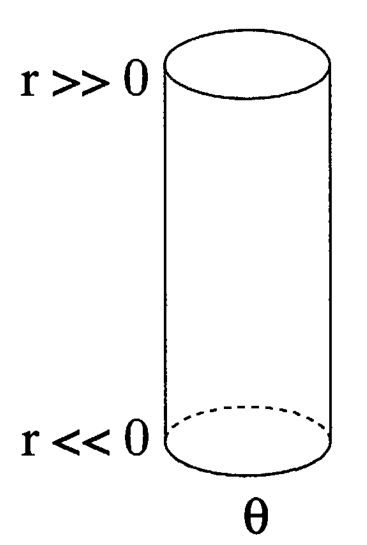
\includegraphics[width=0.28\textwidth]{figs/fig_p192_1.png}
  \caption{$t$ 柱面：顶部标 $r\gg0$（$\sigma$ 模型端），底部标 $r\ll0$（Landau--Ginzburg 端），绕柱圆周为 $\theta$ 角。（原文 Figure 8，p.192）}
  \label{fig:p192-1}
\end{figure}

现在详细考察这两种情形。
对 $k<n$，$\sigma$ 模型的目标空间是 Fano 簇，即 $\mathbf{CP}^{n-1}$ 中次数 $k<n$ 的超曲面。
这在紫外是一个好的描述，给出一个提法恰当的量子场论，其红外行为正是我们想确定的。
红外流把我们带到 $r\ll0$，在那里我们找到两类真空：(1) 中心荷为 $\widehat{c}=n(1-2/k)$ 的共形场论真空；(2) 大 $\sigma$ 处 $n-k$ 个新真空。
大 $\sigma$ 处相应的有效扭曲超势为
\[
\widetilde{\mathcal{W}}_{\rm eff}=t\Sigma+\frac{i}{2\pi}(n-k)(\Sigma-\Sigma\ln\Sigma).
\]
这两类真空的中心荷都小于紫外理论的值 $\widehat{c}=n-2$。
因此在这个例子中，单个紫外量子场论可以流向相当不同的红外可能性。
二维 $\mathcal{N}=2$ $\sigma$ 模型的重整化群流

% ===== 原文 p.193 =====

有许多不变量（例如 $\operatorname{Tr}(-1)^F$、椭圆亏格，以及它们的一些近亲）。
要重现 Fano 目标的紫外 $\sigma$ 模型的不变量，必须对 (1)、(2) 两类红外真空求和。

\subsubsection{$c_1<0$ 的情形}
% 原文 §13.6.5：The case $c_1<0$

现在考虑相反的情形 $k>n$。
$\mathbf{CP}^{n-1}$ 中次数 $k>n$ 的超曲面是一般型代数簇（algebraic variety of general type）。
此时 $\beta>0$，并且不存在一个定义良好的量子场论，其场是从时空到该超曲面的映射。
然而，以该超曲面为目标空间的 $\sigma$ 模型作为红外的有效理论是有意义的。
人们可以问：什么样的定义良好的紫外理论能在红外流到这个有效理论？

对这个问题，下面给出一个答案。
对 $k>n$，柱面的紫外稳定端是 Landau--Ginzburg 端。
Landau--Ginzburg 模型的中心荷为 $\widehat{c}=n(1-2/k)$，当 $k>n$ 时它大于 $\sigma$ 模型的值 $\widehat{c}=n-2$。
因此 Zamolodchikov 定理允许从 LG 模型到 $\sigma$ 模型的重整化群流。
这正是实际发生的，因为当 $n<k$ 时柱面上的重整化群流是「向上」的，即离开 LG 模型、趋向 $\sigma$ 模型。

% [Tutor Note: 这里的方向一致性可用 Zamolodchikov 定理直接自检：$k>n$ 时 $\widehat{c}_{\rm LG}=n(1-2/k)>n-2=\widehat{c}_\sigma$，故只允许 LG（紫外）$\to\sigma$（红外），反向流被禁止；而 $k<n$ 时不等式反转，只允许 $\sigma$（紫外，Fano）$\to$ LG（红外）。换句话说，「哪个端是紫外」完全由 $n-k$ 的符号决定，而不是由柱面上 $r$ 的符号决定——$r\gg0$ 永远对应 $\sigma$ 模型、$r\ll0$ 永远对应 LG，变的只是流的方向。]

若 $k>n$，在柱面的 LG 端没有大 $\sigma$ 真空。
取而代之，有 $k-n$ 个这样的真空伴随着 $\sigma$ 模型。
因此，由 Landau--Ginzburg 模型给出的一个定义良好的紫外不动点，可以在红外流向该超曲面的 $\sigma$ 模型，或流向大 $\sigma$ 处的非经典有质量真空。
正如 $k<n$ 的情形，要想在紫外与红外理论之间等同诸如 $\operatorname{Tr}(-1)^F$ 这样的重整化群不变量，必须对红外极限下的两类真空求和。

\begin{figure}[htbp]
  \centering
  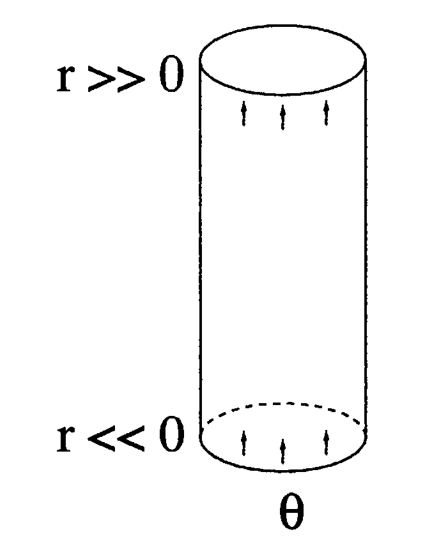
\includegraphics[width=0.28\textwidth]{figs/fig_p193_1.png}
  \caption{$t$ 柱面：与 Figure 8 相同的两个端（$r\gg0$ 在上、$r\ll0$ 在下），但柱面上的箭头改为向上，表示 $k>n$ 时重整化群流沿柱面「向上」，即从 LG 端流向 $\sigma$ 模型端。（原文 Figure 9，p.193）}
  \label{fig:p193-1}
\end{figure}

注意，无论 $n-k$ 的符号如何，非经典真空总是出现在红外而不是紫外。
这有一个很好的直观理由。
在紫外，也就是我们定义理论的地方，我们可以（在所有可能的紫外不动点中）挑选我们想研究的理论，所以紫外理论只有一类真空。
走向红外意味着解方程，而在这个阶段事情就不由我们作主了：一个确定的量子场论对其红外行为可以有不止一个解。
这正是我们今天所发现的。
事实上我们已经看到，一个确定的紫外场论（$k<n$ 时基于 Fano 簇，$k>n$ 时基于 Landau--Ginzburg 模型）可以流向相当不同的红外可能性。

% ===== 原文 p.194 =====

我们今天研究过的 $k\ne n$ 的两种情形都具有相当的方法论意义。
对 $k<n$，我们看到具有 Fano 目标的量子理论一般给出一种混合的答案：既有 Calabi--Yau 流形的行为，又有复射影空间的行为。
对 $k>n$，我们在一个具体情形中找到了一个定义良好的紫外不动点，它流向基于一般型代数簇的有效理论。

\subsection{参考文献与交叉引用}
% 原文 References and cross references

本材料的基本参考文献是
\begin{quote}
E. Witten, \emph{Phases of $\mathcal{N}=2$ SUSY theories in two dimensions}, Nucl. Phys. B \textbf{403} (1993), p.159--222.
\end{quote}

% [Tutor Note: 本页出现的几个交叉引用代号 $[I\text{-}\dots]$、$[II\text{-}\dots]$ 指本丛书第 I 卷（数学部分）与第 II 卷（物理部分）的对应章节，而非本文内部的编号，故原样保留。注意 [I-Renorm Groups] 即第 I 卷中关于重整化群的章节，其缩写为 ``Renorm Groups'' 而非 ``Renormalization Group''，检索时勿按全称拼写。]

CFT 的中心荷这一概念是在 [II-CFT, §2.4] 中引入的，在 [II-Strings] 的第 3 讲中也有讨论。
$\beta$ 函数与重整化群流在 [I-Renorm Groups] 的第 3 讲中有详细讨论。
关于我们可以加进超对称拉氏量的各种可能的项（包括 Fayet--Iliopoulos 项），在 [I-Supersolutions] 第 9 章中给出。

% [Tutor Note: 原文此句有两处排印讹误：一是 ``Fayet-Iliopulous''，正确拼法为 Fayet--Iliopoulos（P. Fayet 与 J. Iliopoulos, Phys. Lett. B 51 (1974) 461）；二是 ``are given is Chapter 9''，介词误作 ``is''，应为 ``in''。译文按正确拼法与语义处理；读者若按原文检索文献，应以 Fayet--Iliopoulos 为准。]

CFT 中极小模型的一个参考文献是
\begin{quote}
W. Boucher, D. Friedan, and A. Kent, \emph{Determinant formulae and unitarity for the $\mathcal{N}=2$ superconformal algebra in two dimensions, or exact results on string compactification}, Phys. Lett. B \textbf{172} (1986), p.~316.
\end{quote}

关于某些 Landau--Ginzburg 模型的红外极限与极小模型之间关系的讨论，见于
\begin{quote}
B. Greene, C. Vafa, and N. Warner, \emph{Calabi--Yau manifolds and renormalization group flows}, Nucl. Phys. B \textbf{324} (1989), p.~371--390.\\
E. Martinec, \emph{Criticality, catastrophes and compactifications}, in: L. Brink et al., eds., \emph{Physics and Mathematics of Strings}, World Scientific, 1990, p.~389--433.
\end{quote}

关于这一论断的更多证据见第 15 讲。

GIT（几何不变量理论，geometric invariant theory）的基本参考文献，以及关于 flop 在辛约化（symplectic reduction）背景下如何出现的文献，是
\begin{quote}
D. Mumford, J. Fogarty, and F. Kirwan, \emph{Geometric Invariant Theory}, Springer-Verlag, 1994.\\
V. Guillemin and S. Sternberg, \emph{Birational equivalence in the symplectic category}, Invent. Math \textbf{97} (1987), p.~485.\\
P. Aspinwall, B. Greene, and D. Morrison, \emph{Calabi--Yau moduli space, mirror manifolds and spacetime topology change in string theory}, Nucl. Phys. B \textbf{416} (1994), p.414--480.
\end{quote}

Zamolodchikov 定理的参考文献是
\begin{quote}
A. B. Zamolodchikov, \emph{`Irreversibility' of the flux of the renormalization group in a 2-D field theory}, JETP Lett. \textbf{43} (1986), pp.~730--732; Pisma Zh. Eksp. Teor. Fiz. \textbf{43} (1986), pp.~565--567. (Reprinted in Itzykson, C. (ed.) et al., \emph{Conformal invariance and applications to statistical mechanics}, pp.~702--704.)
\end{quote}


\clearpage
% 原文 pp.195–201（印刷 pp.1313–1319）
\section{Lecture 14：二维 $\mathcal{N}=2$ 超对称理论（二）：手征环与扭曲理论}

\begin{keytakeaways}
本讲在二维 $\mathcal{N}=2$ 超对称理论中取定一个超荷 $Q$，把手征环（chiral ring）定义为局部算符的 $Q$ 上同调，并证明 $Q$-闭算符的「后代」在闭链上的积分给出与度规无关、因而具有拓扑意义的关联函数。
核心数学工具是 $R$ 对称性的规范化与「扭曲」：把旋转生成元改成 $K'=K\pm\frac12J_L\pm\frac12J_R$，使 $Q$ 在任意超 Riemann 曲面上都是整体超对称；可规范化的组合只有 $J_L\pm J_R$，其判据是反常系数二次型在这两个零向量上为零（$k=0$）。
物理图像是：扭曲之后理论成为拓扑场论，路径积分只依赖 $Q$ 的不动点集——纯 $\mathcal{N}=2$ 规范理论给出平坦联络模空间上的示性类积分，Kähler $\sigma$ 模型给出量子上同调中的积分。
主要结论是：$Q$ 上同调类不依赖插入点的位置，故手征环是 $\mathbb{Z}/2\mathbb{Z}$ 分次交换环；在 Hamilton 框架下 $H=\{Q,\widetilde Q\}$、$H^*(Q)=\ker Q/\operatorname{Im}Q$，当 $H$ 有离散谱时它等同于零能态空间。
\end{keytakeaways}

% ===== 原文 p.195 =====
% 原文页眉：LECTURE 14；标题：$N=2$ SUSY Theories in Dimension Two, Part II: Chiral Rings and Twisted Theories

本讲再次讨论二维的 $\mathcal{N}=2$ 超对称理论。
取其中一个超对称 $Q$，我们将对定义在平坦闵可夫斯基空间或欧氏空间中的理论，
定义局部算符的手征环（chiral ring）与态的 $Q$ 上同调（$Q$-cohomology）。
接着我们讨论如何扭曲（twist）理论，使超对称 $Q$ 至少在一大类 $2|4$ 维超流形（supermanifold）上具有整体意义。
一旦 $Q$ 在 $\Sigma$ 上的某个理论中被整体化（globalize），我们便有了该理论的「手征局部算符环」这一概念。
我们可以定义所谓 $Q$ 不变算符的后代（descendants），
并证明：这些后代在流形中各闭链上的积分给出具有拓扑意义的关联函数。
为计算这些函数，人们对 $Q$ 不变的场作积分。

随后我们详细考察两个带整体超对称 $Q$ 的扭曲理论的例子。
第一个是二维的、规范群为单 Lie 群 $G$ 的纯 $\mathcal{N}=2$ 规范理论。
在这里我们看到，手征函数（chiral functions）之环被等同于 Lie 代数上的不变多项式（invariant polynomial）。
经典地，$Q$ 不变态的空间就是通常的平坦联络（flat connection）空间
（在联络可约（reducible）的情形，还要加上伴随丛（adjoint bundle）的一个额外平行截面）。
$Q$ 不变算符的关联函数被等同于：由 Lie 代数中的不变多项式导出的那些通常类，
在平坦联络模空间上的积分。（可约联络会带来额外的复杂性。）

第二个例子是映入 Kähler 流形的 $\mathcal{N}=2$ 超对称二维 $\sigma$ 模型。
结果表明，存在一种扭曲方式，它给出的手征环正是该 Kähler 流形的拓扑上同调（topological cohomology）。
$Q$ 不变态的空间是从 Riemann 曲面到 $X$ 的全纯映射（holomorphic map）空间。
在这个扭曲理论中，计算拓扑关联函数的路径积分正是量子上同调（quantum cohomology）中的积分。
当 Kähler 流形是 Calabi--Yau 流形时，还有第二种不等价的扭曲方式，它给出一个不同的理论。
在该理论中，手征环是 $H^*(X,\wedge^*T^{1,0}(X))$，
而 $Q$ 不变的场是从 Riemann 曲面到 $X$ 的常映射。
于是，计算拓扑关联函数的路径积分就是这些对象在 $X$ 上的积分——
这些积分与 $X$ 上 Hodge 结构的形变（variation of Hodge structure）有关。

\noindent\textit{（本讲笔记由 John Morgan 整理。原文 p.1313 页脚）}

% [Tutor Note: 这里的 $H^*(X,\wedge^*T^{1,0}(X))$ 用的是全纯**切**丛 $T^{1,0}$ 的外幂，而不是通常写 Hodge 分解时用的全纯余切丛 $\Omega^p=\wedge^pT^{*(1,0)}$，抄写时极易在这一步出错。对 Calabi--Yau 流形，$K_X$ 平凡给出 $\wedge^pT^{1,0}\cong\Omega^{\,n-p}$（$n=\dim_{\mathbb C}X$），故二者作为分次向量空间的总和相同，只是标号 $p\leftrightarrow n-p$ 互换——这正是作者说这些积分「与 Hodge 结构的形变有关」的原因。另可注意：本页先后描述的两种扭曲即今称的 A 模型（手征环 $=H^*(X)$，态 $=$ 全纯映射）与 B 模型（手征环 $=\oplus_{p,q}H^q(X,\wedge^pT^{1,0})$，态 $=$ 常映射），二者的差别仅是 $K'$ 中 $J_R$ 前的符号。]

% [Tutor Note: 原文此处写 "the ring of chiral functions"，按上下文（同页前面说的是 chiral ring of local operators）应读作「手征算符之环」；"functions" 一词沿用了作者在讨论超势时对「超场的函数」的习惯说法，并非指普通函数。译文按「手征函数之环」直译以免改动原文，但读者须知它指的是算符的环。]

% ===== 原文 p.196 =====
\subsection{$R$ 对称性再论}
% 原文 §14.1：R-symmetry revisited

我们所考察的大多数 $\mathcal{N}=2$ 超对称例子都将（至少在经典层面）同时具有左行与右行的 $R$ 对称性——
即上一讲中记作 $J_L$ 与 $J_R$ 的那些 $R$ 对称性。
只用其中一个 $R$ 对称性也可以完成今天的讨论，但至少必须有一个。
不过，我们仍将假定 $R$ 对称性群是 $U(1)\times U(1)$，从而 $J_R$ 与 $J_L$ 兼备。
理论定义所在的超流形是 $\mathbb{R}^{2|4}$。
我们最终还将允许某一类带欧氏度量的分裂（split）$2|4$ 维超 Riemann 曲面
（以及带平坦闵可夫斯基度量的 $2|4$ 维超流形）。
奇方向的空间是 $J_L$ 的二维表示的一份拷贝与 $J_R$ 的二维表示的一份拷贝。
我们预期 $J_L$ 与 $J_R$ 之间存在由世界面定向反转给出的对称性。

我们可以对 Lagrange 量的一个对称性尝试做的一种操作，是把它规范化（gauge）。
若待规范化的对称群是 $H$，则新的 Lagrange 量将含有规范群为 $H$ 乘以原理论规范群（若有）的规范场。
直观上，规范化过程就是把取值于一个常空间的场，换成取值于一个 $H$-丛的场，并添加一个新场——$H$-联络。
当作用量或 Lagrange 量是某个局部 Lagrange 密度的积分时，规范化最为直接。
此时在经典层面总可以构造出新的、已规范化的 Lagrange 量：把 Lagrange 量中的普通导数换成协变导数。
往往存在一种自然的做法来完成这一过程；但无论如何，对对称性作规范化的不同选择
所得到的 Lagrange 量之间只差规范不变项。
然而还有一个问题：规范化后的理论作为量子理论是否有意义。
若原理论具有这一性质，那么（在我们所处维数足够低、不会因规范化而遭遇新的紫外困难的前提下）
规范化后的理论也具有该性质的充要条件是：某些反常（anomaly）必须相消。

在我们的情形中，永远不可能把整个 $U(1)\times U(1)$ 的 $R$ 对称性群规范化，
而得到一个作为量子理论有意义的结果。
事实上，能以这种方式规范化的 $J_L$ 与 $J_R$ 的组合只有 $J_L\pm J_R$。
它们被称为矢量流与轴矢流：
\[
\begin{aligned}
J_V &= J_L+J_R,\\
J_A &= J_L-J_R.
\end{aligned}
\]
若其中之一被规范化，另一个就会出现反常，不再是量子理论的对称性。
为说明这一点，我们需要关于反常的一些一般性观察。
说一个理论具有由流 $J_L$ 生成的对称性，意思是关联函数满足恒等式
\[
d_x\bigl\langle J_L(x)\mathcal{O}(y_1)\dots\bigr\rangle=0 \qquad (\ast)
\]
只要 $x$ 与各 $y_i$ 不同。这里 $d_x$ 是对 $x$ 变量的外微分。
若把关联函数（作为分布）延拓穿过对角线，这个恒等式会多出支撑在对角线上的项。
一个非常重要的特例是流本身的两点函数（或者，在 $2k$ 维时空中是 $(k+1)$ 点函数）。
对此，一般结构是
\[
d_x\bigl\langle J_L(x)J_L(y)\bigr\rangle=\frac{k}{2\pi}d_y\delta(x-y) \qquad (\ast\ast)
\]

% [Tutor Note: $(\ast\ast)$ 中的系数 $\frac{k}{2\pi}$ 依赖流的归一化，切勿与「级」（level）混为一谈：若把 $J_L$ 重新标度 $J_L\to cJ_L$，则 $k\to c^2k$。真正有物理意义、且在下页被用到的是 $k$ 的整性（p.197 所谓「满足一个整性条件」）；在二维共形场论中它就是 $U(1)$ 流的量子化级，故「$k=0$ 才可规范化」等价于「级为零才无反常」。另请注意作者用「$2k$ 维时空中的 $(k+1)$ 点函数」一句概括了一般维数的反常：$dJ$ 的对角项在四维表现为三点函数（三角形图），在二维表现为两点函数，后者正是下一段 $dJ_L=\frac{k}{2\pi}F$ 的来源。]

% [Tutor Note: 原文作 "The supermanifold on which the theory is defined in $\mathbf{R}^{2|4}$"，其中的介词 "in" 显然是 "is" 之误（试与下一句 "We shall also eventually allow…" 对照）。译文按「理论定义所在的超流形是 $\mathbb{R}^{2|4}$」处理；此处若照字面读成「定义在 $\mathbb{R}^{2|4}$ 中」虽不影响物理，却会漏掉作者正在引入「超流形」这一几何框架的用意。]

% ===== 原文 p.197 =====
其中 $k$ 是某个常数，它可以为零，也可以不为零。
生成 $J_L$ 的整体对称性可被规范化的条件，恰恰是 $k=0$。
为看清这一点，让我们试着通过向理论中添加一个 $U(1)$ 规范场 $A$ 来规范化该对称性。
Lagrange 量获得一个额外项 $\int A\wedge J_L$。
（若 $J_L$ 本身含有带荷场的导数，还可能有更多项，即 $A$ 的高阶项。）
现在，我们要判断带这个耦合的理论是否真的具有由 $J_L$ 生成的对称性，
即恒等式 $(\ast)$ 对这个理论是否成立。
为此我们必须在原理论中考察
\[
d_x\left\langle J_L(x)\mathcal{O}(y_1)\dots\exp\left(\int A\wedge J_L\right)\right\rangle.
\]
引入指数是为了用原理论来表达新理论的关联函数。
若把它按 $A$ 的幂展开，则线性于 $A$ 的项在利用 $(\ast\ast)$ 并分部积分之后给出
\[
\bigl\langle \mathcal{O}(y_1)\cdots kF(x)\bigr\rangle,
\]
其中 $F=dA$ 是曲率。这可以写成一个算符关系
\[
dJ_L=\frac{k}{2\pi}F,
\]
它断言：规范化之后，$J_L$ 不再生成对称性。

更一般地，若有若干流 $J^1,\dots,J^s$ 生成 $s$ 维的 Lie 群 $G$，其 Lie 代数为 $\mathcal{G}$，
则两点函数满足
\[
d_x\bigl\langle J^a(x)J^b(y)\bigr\rangle=\frac{k^{ab}}{2\pi}d_y\delta(x-y),
\]
其中 $k^{ab}$ 是 $\mathcal{G}$ 上某个不变二次型。
二次型 $k$ 没有正定性（例如左行与右行无质量费米子的贡献符号相反），但确实满足一个整性条件。
若我们规范化 $G$ 的一个子群 $H$，其 Lie 代数为 $\mathcal{H}$，
则按与上面类似的推理，量子理论只有在二次型 $k$ 限制到 $\mathcal{H}$ 上为零时才有意义。
若确实如此，则规范化后理论的「整体对称性」由 $\mathcal{H}^{\perp}/\mathcal{H}$ 中的流生成，
也就是 $\mathcal{G}$ 中与 $\mathcal{H}$ 正交的流，模去 $\mathcal{H}$ 中的那些流。

在我们将要考察的 $\mathcal{N}=2$ 理论中有两个流 $J_L,J_R$，
并且存在一个交换 $J_L$ 与 $J_R$ 的「宇称」对称性（即二维时空的定向反转）。
$k$ 在定向反转下为奇，故在这种情形下 $k$ 的结构是
$k^{LL}=-k^{RR}\neq0$、$k^{LR}=0$。
这个二次型有两个零向量 $J_L\pm J_R$，
因此这两个 $R$ 对称性的线性组合中任何一个都可以被规范化。
若其中一个被规范化，第二个就变得「反常」——它不再守恒——
因为这两个零向量当然并不彼此正交。
「幸运的是」，这些选项与我们在下面因其他理由所需要的选择一致。

我们真正感兴趣的并不只是规范化，而是用 $R$ 对称性来扭曲理论。
这一过程要求先规范化 $R$ 对称性，然后用一个从度规所决定的正交群到对称群的同态来扭曲它。
结果表明，进行这一过程将有两种等价的方式。
但在着手扭曲之前，我们必须先理解局部的情形。那是下一节的主题。

% [Tutor Note: 「两个零向量并不彼此正交」可以一行算出：设 $k^{LL}=k_0$、$k^{RR}=-k_0$、$k^{LR}=0$，则 $k(J_L+J_R,J_L-J_R)=k_0+k_0=2k_0\neq0$，而 $k(J_L\pm J_R,J_L\pm J_R)=k_0-k_0=0$，故 $J_L\pm J_R$ 都是零向量、却互不正交。正是这个非零内积使得「规范化其中一个 $\Rightarrow$ 另一个反常」：规范场 $A_\pm$ 的混合 Chern--Simons 型项（在二维就是 $A_+A_-$ 型的质量项）会破坏另一条流的守恒。作者说「幸运的是这些选项与下面所需一致」，指的是 §14.3 中要规范化的恰是 $K'=K\pm\frac12J_L\mp\frac12J_R$ 所对应的组合，即 $J_L$ 与 $J_R$ 的同号/反号线性组合。]

% [Tutor Note: $\mathcal{H}^{\perp}/\mathcal{H}$ 这一写法容易读错：这里「正交」是对不变二次型 $k$ 而言的，而非对 Killing 形式；当 $k$ 在 $\mathcal{H}$ 上退化时（本讲正是如此），$\mathcal{H}^\perp$ 严格大于 $\mathcal{H}$，商空间才给出真正的「剩余整体对称性」。另注意 $\mathcal{H}^{\perp}$ 必须理解为 $\{X\in\mathcal{G}\,|\,k(X,Y)=0\ \forall Y\in\mathcal{H}\}$，而不是 $\mathcal{G}$ 中与 $\mathcal{H}$ 对易的子代数——两种「正交」在这里给出不同的答案。]

% ===== 原文 p.198 =====
\subsection{算符的 $Q$ 上同调}
% 原文 §14.2：Q-cohomology of operators

我们考虑带标准欧氏或闵可夫斯基度量的 $\mathbb{R}^{2|4}$。
设我们的二维 $\mathcal{N}=2$ 超对称理论具有如下超对称性：
\begin{center}
\begin{tabular}{c|c}
\hline
$U(1)_L$ 的特征标 & $U(1)_R$ 的特征标\\
\hline
$Q_-$ & $Q_+$\\
$\overline{Q}_-$ & $\overline{Q}_+$\\
\hline
\end{tabular}
\end{center}
$Q_-$ 与 $\overline{Q}_-$ 在 $U(1)_L$ 的标准表示及其共轭表示中变换，并与 $U(1)_R$ 对易；
而 $Q_+$、$\overline{Q}_+$ 与 $U(1)_R$ 及 $U(1)_L$ 的关系类似。
这些超对称满足关系
\[
Q_+^2=\overline{Q}_+^2=0,\qquad \{Q_+,\overline{Q}_+\}=P_+,
\]
以及把 $+$ 换成 $-$ 的对称关系。此外，
\[
\{Q_+,Q_-\}=\{\overline{Q}_+,Q_-\}=\{Q_+,\overline{Q}_-\}=\{\overline{Q}_+,\overline{Q}_-\}=0.
\]
我们将同时考虑四种密切相关的可能性。令 $Q$ 为下列之一：
\[
Q_++Q_-,\qquad Q_++\overline{Q}_-,\qquad \overline{Q}_++Q_-,\qquad \overline{Q}_++\overline{Q}_-.
\]
（前两种可能性给出不等价的扭曲理论；后两种是前两种的厄米共轭，会给出等价的理论。）
为固定记号，我们这样选取生成元，使得 $Q=Q_++Q_-$。
令 $\mu=\pm$，我们看到 $P_\mu$ 可以写成一个对易子
\begin{equation}
  \tag{14.1}
  \label{eq:14-1}
  P_\mu=\{Q,T_\mu\},
\end{equation}
其中 $T_\mu$ 是 $Q_\pm,\overline{Q}_\pm$ 的一个线性组合。
我们感兴趣的是 $Q$ 作为微分（通过取超括号（superbracket）作用）在局部算符空间上
（更一般地，作用在这类算符的乘积上）的上同调。
于是，一个局部算符 $\phi(x)$ 若满足 $Q$-闭，即 $\{Q,\phi(x)\}=0$，就定义一个 $Q$ 上同调类。
用式 14.1 作一个简单计算即可看出，对 $Q$-闭算符 $\phi(x)$ 我们有
\[
d_\mu\phi=\{Q,[T_\mu,\phi]\}.
\]
这个等式意味着算符 $d\phi$ 是 $Q$-恰当的（$Q$-exact），
因而 $d\phi$ 在算符的 $Q$ 上同调类空间中的类为平凡。
这意味着：当我们改变 Riemann 曲面上的点 $x$ 时，局部算符 $\phi(x)$ 的 $Q$ 上同调类不变。
由此可知，在 $Q$ 上同调中这类 $Q$-闭局部算符彼此对易——只需把点移到类空间隔即可。
也就是说，算符的 $Q$ 上同调空间是一个 $\mathbb{Z}/2\mathbb{Z}$ 分次交换环。
我们总可以用 $0$-形式算符来代表这些算符。
这是「$Q$ 上同调类不依赖于度规」与「$Q$ 上同调类具有微分同胚不变性」这两件事的容易推论。
这些事实将在后面建立。

让我们回顾一个先前在第 11 讲 §11.3 中见过的构造。
给定一个 $Q$ 不变的 $0$-形式局部算符 $\phi=\phi^{(0)}$，我们定义一个 $1$-形式局部算符
\[
\phi^{(1)}_\mu=[T_\mu,\phi^{(0)}].
\]

% [Tutor Note: 作者的「简单计算」实为分次 Jacobi 恒等式：设 $Q$ 奇、$T_\mu$ 偶、$\phi$ 偶，则 $\{Q,[T_\mu,\phi]\}=[\{Q,T_\mu\},\phi]-[T_\mu,\{Q,\phi\}]$；只有当 $\{Q,\phi\}=0$（即 $\phi$ 为 $Q$-闭）时第二项才消失，从而得到 $d_\mu\phi=\{Q,[T_\mu,\phi]\}$。因此这条恒等式**只对 $Q$-闭算符**成立——作者紧接着就强调 $\phi$ 是 $Q$-closed，正是为此。若误把它当成对任意 $\phi$ 都成立的算符恒等式，就会错误地断言「所有」算符的上同调类都与位置无关。另外，要同时得到 $P_+$ 与 $P_-$ 的恰当性，(14.1) 中的 $Q$ 必须兼含 $Q_+$ 与 $Q_-$ 两种手征性；若只取单个 $Q_+$，则只有 $P_+$ 是恰当的，$\phi$ 便只能沿一个光锥方向平移，「上同调类与位置无关」也就不再成立。]

% ===== 原文 p.199 =====
以及
\[
\phi^{(1)}=\phi^{(1)}_\mu dx^\mu.
\]
与上一段所做的同样的计算表明
\[
d\phi^{(0)}=\{Q,\phi^{(1)}\}.
\]
这意味着：若 $\Sigma_1$ 是超 Riemann 曲面中的一个一维闭链（one-cycle），则
\[
\int_{\Sigma_1}\phi^{(1)}
\]
是 $Q$ 不变的。令 $\phi^{(2)}=[T,\phi^{(1)}]$。则
\[
d\phi^{(1)}=\{Q,\phi^{(2)}\}.
\]
因此 $\int_{\Sigma_2}\phi^{(2)}$ 是 $Q$ 不变的。
于是，以这种方式，从一个 $Q$ 不变的 $0$-形式局部算符 $\phi^{(0)}$ 出发，
我们可以构造出一族 $k$-形式局部算符 $\phi^{(k)}$，称为 $\phi^{(0)}$ 的后代，
从而得到更一般的 $Q$ 不变算符，其形式为
\[
\int_{\Sigma_k}\phi^{(k)},
\]
其中 $\Sigma_k$ 是 $\Sigma$ 中的一个 $k$ 维闭链。
我们的计算表明，对任何 $Q$ 不变的局部算符 $\phi^{(0)}$，
算符 $\phi^{(0)}+\phi^{(1)}+\phi^{(2)}$ 对总微分 $d-Q$ 是闭的。

这个「下降」（descent）程序在第 11 讲中也曾采用，那是在二维规范理论的背景下。

\subsection{扭曲理论以赋予其整体意义}
% 原文 §14.3：Twisting the theory to give it global meaning

到目前为止，我们一直在带固定坐标的 $\mathbb{R}^{2|4}$ 上工作。
如果我们旋转空间，则 $Q=Q_++Q_-$ 并非不变。
我们的目标是修改事物，直到 $Q$ 在旋转下不变，从而可以定义在更一般的欧氏 $2|4$ 维流形上。
让我们把欧氏旋转群记作 $SO(2)_E$。
欧氏理论中我们可支配的整个对称群是 $SO(2)_E\times U(1)_L\times U(1)_R$。
这个群到 $SO(2)_E$ 有显然的投影，并有一个回到第一个因子的分裂。
我们希望找到这个投影映射的另一个分裂，即乘积内部的一个群 $SO(2)'_E$，
它同构地投影到 $SO(2)_E$ 上，但具有与 $Q$ 对易这一额外性质。
容易看出，这样的分裂存在且唯一；它在 Lie 代数层面由
\[
K'=K\pm\frac12J_L\pm\frac12J_R
\]
给出，其中 $K$ 是 $SO(2)_E$ 的生成元，而符号取决于我们为 $Q$ 选定了四种可能性中的哪一种。
在我们集中关注的 $Q=Q_++Q_-$ 的情形，有
\[
K'=K+\frac12J_L-\frac12J_R.
\]
这些公式中出现 $1/2$ 这一事实意味着：扭曲实际上涉及 $SO(2)_E$ 的自旋形式（spin form）。

请注意，为了在 $n$ 维中做这样的扭曲，必须存在从 $\mathrm{Spin}(n)$ 到 $R$ 对称群的非平凡同态。
在二维，当 $R$ 对称群为 $U(1)$ 时（例如 $\mathcal{N}=1$ 超对称）就可以做到这一点。
但对 $n=4$，则必须有 $\mathcal{N}=2$ 超对称，

% [Tutor Note: 「容易看出这样的分裂存在且唯一」可以显式验证。设 $K'=K+aJ_L+bJ_R$，并要求 $[K',Q_++Q_-]=0$：由 $[K,Q_\pm]=\pm\frac12Q_\pm$、$[J_L,Q_-]=Q_-$、$[J_R,Q_+]=Q_+$（其余为零），$Q_+$ 分量给出 $\frac12+b=0$、$Q_-$ 分量给出 $-\frac12+a=0$，故 $a=\frac12$、$b=-\frac12$，即 $K'=K+\frac12J_L-\frac12J_R$，与文中一致；若改用 $Q_++\overline{Q}_-$，则 $b$ 变号而 $a$ 不变，得到 $K'=K+\frac12J_L+\frac12J_R$——这正是两种不等价扭曲（今称 A 模型与 B 模型）的来源。注意 $J_L,J_R$ 的荷归一化在这里必须取 $\pm1$ 而非 $\pm\frac12$，否则 $a,b$ 会差一个因子 2；这个归一化与 p.198 表格中「标准表示及其共轭」的说法相配。]

% [Tutor Note: 「涉及 $SO(2)_E$ 的自旋形式」这句话的后果常被低估：$K'$ 的半整数本征值意味着扭曲后的理论依赖自旋结构的选择，两种自旋结构给出的理论相差 $(-1)^F$——这也是为什么 p.200 要从「带选定自旋结构的 Riemann 曲面」出发。又，$n=4$ 时 $R$ 对称群必须是 $SU(2)\times U(1)$，因为只有 $SU(2)$ 才有来自 $\mathrm{Spin}(4)\cong SU(2)\times SU(2)$ 的非平凡同态；这一句是理解四维 Donaldson 理论如何作为 $\mathcal{N}=2$ 超对称规范理论的扭曲而出现的关键。]

% ===== 原文 p.200 =====
使得 $R$ 对称群为 $SU(2)\times U(1)$，而它才有来自 $\mathrm{Spin}(4)$ 的非平凡同态。

有了这些预备讨论，我们现在可以整体化我们关于局部算符的 $Q$ 上同调类的理论。
假设我们有一个局部以 $\mathbb{R}^{2|4}$ 为模型的 $2|4$ 维超 Riemann 曲面。
给定任何带有选定自旋结构的普通（玻色）Riemann 曲面，
都有相应的一个非常简单的超 Riemann 曲面：它是一个分裂的 $2|4$ 维复流形，其奇方向为
\[
\bigl(\Pi K^{1/2}\oplus\Pi\overline{K}^{1/2}\bigr)\oplus
\bigl(\Pi\overline{K}^{1/2}\oplus\Pi K^{1/2}\bigr).
\]
这里 $\theta^+,\overline{\theta}^+$ 是前两个线丛的截面，而 $\theta^-,\overline{\theta}^-$ 是后两个线丛的截面。
现在，我们将通过「扭曲」改变这个超流形的奇部。
我们把包含 $\theta^\pm$ 的自旋丛乘以典范丛（canonical bundle）平方根的 $\pm1/2$ 次幂来扭曲。
扭曲的结果是把上述线丛替换为
\[
\bigl(\Pi\mathcal{O}\oplus\Pi K\bigr)\oplus\bigl(\Pi\mathcal{O}\oplus\Pi\overline{K}\bigr),
\]
并使超对称
\[
Q=\frac{\partial}{\partial\theta^+}+\frac{\partial}{\partial\theta^-}
\]
成为一个整体对称性。
局部地，这个对称性与我们在 $\mathbb{R}^{2|4}$ 上一直讨论的对称性 $Q$ 一致。
任何一般地可以在超 Riemann 曲面上表述的 $\mathcal{N}=2$ 理论，
在被表述在我们刚刚描述的那类特殊超 Riemann 曲面上时，都将以 $Q$ 为对称性。
这保证了扭曲理论的整体版本存在；当然，它可以按分量场（component field）显式描述。

一旦我们把超对称 $Q$ 整体化，先前所有的讨论都可以整体化。
特别地，对一个 $Q$-闭局部算符 $\mathcal{O}(p)$，$\mathcal{O}(p)$ 的 $Q$ 上同调类与点 $p$ 无关。
于是，这个整体超 Riemann 曲面上的局部算符的 $Q$ 上同调类
生成一个 $\mathbb{Z}/2\mathbb{Z}$ 分次交换环，称为该理论的手征环。

\subsubsection{某些关联函数及其基本性质}
% 原文 §14.3.1：Certain Correlation Functions and Their Basic Properties

我们将考虑下列类型的路径积分：
\[
Z_{(\mathcal{O}_\alpha)}=\int D\Phi\,e^{-\mathcal{L}}
\prod_{\alpha=1}^{n}\int_{\Sigma_\alpha}\mathcal{O}_\alpha^{(k_\alpha)},
\]
其中对每个 $\alpha$，算符 $\mathcal{O}_\alpha$ 是 $Q$-闭局部算符，$k_\alpha=0,1,2$，
而 $\Sigma_\alpha$ 是超 Riemann 曲面 $\Sigma$ 中的一个 $k_\alpha$-维闭链。

以下是 $Z_{(\mathcal{O}_\alpha)}$ 的基本性质。

1). 它与超 Riemann 曲面上的度规无关。
理由是：当你把度规作 $\delta g$ 的变动时，你插入 $\int_\Sigma \delta g\cdot T$，其中 $T$ 是应力-能量张量。
但正如我们先前所见，$T$ 在如下意义上是 $Q$-恰当的：存在场 $S_{\mu\nu}$ 使 $T_{\mu\nu}=\{Q,S_{\mu\nu}\}$。
于是我们看到，这个插入产生一个形如 $\{Q,\cdot\}$ 的项。
这种项的路径积分为零，因为场是 $Q$ 不变的。
（还请注意到，必须假定 $Q$ 保持路径积分中的测度。若原理论是超对称的，
且流 $\frac12J_L-\frac12J_R$ 可被规范化，则情况确实如此。）

% [Tutor Note: 这里把「度规变动给出 $\int\delta g\cdot T$」当作显然，其实用到了两件事：(i) $T_{\mu\nu}$ 定义为作用量对度规的变分，即 $\delta S=\frac{1}{2}\int\sqrt{g}\,\delta g^{\mu\nu}T_{\mu\nu}$，与符号约定相差一个整体因子；(ii) 在二维，$T_{\mu\nu}$ 还有 Belinfante 改进（improvement）的任意性，而 $\{Q,S_{\mu\nu}\}$ 这一表述挑出了与超共形代数相容的那一个「改进后」的应力张量。另外，括号里「$Q$ 保持测度」这一点不可省：若该 $R$ 流有反常，路径积分测度在 $Q$ 下并不保持不变，$\{Q,\cdot\}$ 的积分就不再为零，本节所有结论都会失效——这正是前两节花大力气讨论 $k=0$ 的原因。]

% [Tutor Note: $(\Pi K^{1/2}\oplus\Pi\overline{K}^{1/2})\oplus(\Pi\overline{K}^{1/2}\oplus\Pi K^{1/2})$ 到 $(\Pi\mathcal{O}\oplus\Pi K)\oplus(\Pi\mathcal{O}\oplus\Pi\overline{K})$ 的替换，暗含了对两组奇坐标取**相反**的扭曲幂次：用 $\overline{K}=K^{-1}$ 可验，第一组 $(\theta^+,\overline{\theta}^+)$ 须乘 $K^{-1/2}$ 才能给出 $(\mathcal{O},K)$，而第二组 $(\theta^-,\overline{\theta}^-)$ 须乘 $K^{+1/2}$ 才能给出 $(\mathcal{O},\overline{K})$；若对两组用同一符号，就会得到 $K^{-1}$ 这种没有整体截面的丛，扭曲后的 $Q$ 也就不再整体定义。原文「to the power $\pm1/2$」中的 $\pm$ 正是此意，极易读漏。又，$\Pi$ 表示把纤维的奇偶性翻转（偶丛变奇丛），它保证 $\theta$ 是反对易的；$\mathcal{O}$ 指结构层。]

% ===== 原文 p.201 =====
（接上页：关联函数与度规无关这一事实的一个重要推论是：
$0$-形式算符 $\mathcal{O}^{(0)}_\alpha$ 必须是标量算符，即自旋为零；
自旋更高的对象在局部旋转下不会不变，它们在关联函数中的插入也就不可能与度规无关。）

2). 它与 $\mathcal{L}$ 中大多数参数无关。
首先，关联函数与任何形如 $\int d^2y\,d^4\theta(\cdots)$ 的项无关。
理由是：为计算这样的项，我们要对全部四个 $Q$ 求导，因此任何这样的项都具有 $\{Q,\dots\}$ 的形式。
带这种插入的积分因与上一段相同的理由而为零。
同理，取决于我们使用的是 $Q_+,Q_-,\overline{Q}_+,\overline{Q}_-$ 中的哪个组合，
项
\[
\int d^2y\,d\theta^+\,d\theta^-\,W+{\rm c.c.}
\]
与
\[
\int d^2y\,d\overline{\theta}^+\,d\theta^-\,\widetilde{W}+{\rm c.c.}
\]
中只有一个可能是非平凡的。
事实上，关联函数与其中之一无关，而对另一个全纯地变化。

3). 我们可以用施于 $Q$ 的作用的不动点定理来计算 $Z_{(\mathcal{O}_\alpha)}$。
我们把 $Q$ 看作（无穷小地）作用在理论中所有场的函数空间上。
若这个作用没有不动点，则路径积分的值为零。
一般地，我们可以把计算归结为对 $Q$ 的不动点集的积分。
这些当然就是那些在超对称 $Q$ 下不变的场位形。

\subsubsection{态的 $Q$ 上同调}
% 原文 §14.3.2：Q-cohomology of States

现在我们从局部算符、路径积分与关联函数的世界，转到 Hamilton 框架。
我们的 Riemann 曲面现在是柱面 $S^1\times\mathbb{R}$。
我们把所有相关的自旋丛在 $S^1$ 上平凡化。
我们有圆周上量子理论的态空间 $\mathcal{H}$，以及 $\mathcal{H}$ 上与时间平移相联系的 Hamilton 算符 $H$。
由于 $Q$ 作用于理论，它在 $\mathcal{H}$ 上产生一个算符（我们也称之为 $Q$），与 $H$ 对易。
此外，由超代数中的对易关系我们看到
\[
H=\{Q,\widetilde{Q}\},
\]
其中 $\widetilde{Q}$ 是 $Q$ 的伴随。当然，我们仍有关系 $Q^2=0$，
因此可以取 $Q$ 对 $\mathcal{H}$ 的作用的上同调：
\[
H^*(Q)=\ker Q/\operatorname{Im}Q.
\]
若我们的理论足够好，使得 $H$ 具有离散谱，则 $H^*(Q)$ 可等同于 $\{\psi\,|\,H\psi=0\}$。
（我们稍后要讨论的规范理论例子并非如此，但对 $\sigma$ 模型成立。）
一般地，$H^*(Q)$ 按 $U(1)\times U(1)$ $R$ 对称性群的作用而双分次。

% [Tutor Note: 两个 F 项的测度并不相同：第一个是通常的 $\int d^2y\,d\theta^+d\theta^-W$，第二个是「扭曲」F 项 $\int d^2y\,d\overline{\theta}^+d\theta^-\widetilde{W}$（注意是 $\overline{\theta}^+$ 配 $\theta^-$，且超势带波浪号），它正是第 13 讲中扭曲超势 $\widetilde{\mathcal{W}}_{\rm eff}$ 所对应的项。千万不要因为「看起来不对称」而擅自改成 $d\overline{\theta}^+d\overline{\theta}^-$，否则该项将不再是对任何 $Q$ 都恰当的恰当形式。一般地，$\int d^4\theta$ 型的项对四个超荷全部求导，故对四种 $Q$ 都是 $\{Q,\cdot\}$；而两个 F 项各自只对其中两个超荷恰当，所以对给定的 $Q$ 只有一个能存活，另一个则全纯地依赖于参数——这正是作者说「一个无关、另一个全纯变化」的含义。]

% [Tutor Note: $H=\{Q,\widetilde{Q}\}$ 中的 $\widetilde{Q}$ 是 $Q$ 的伴随，但它**不是** $Q$ 本身，也未必是同一扭曲理论所保持的超荷：若 $Q=Q_++Q_-$，则 $Q^\dagger=\overline{Q}_++\overline{Q}_-$，这正是 §14.2 列举的第三种组合，而两种扭曲理论一般并不等价。扭曲理论通常还是非正定的（$K'$ 不是任何算符的伴随），故 $H$ 未必有下界；把 $H^*(Q)$ 等同于零能态除了 $Q^2=0$ 之外，还需要「$H$ 有离散谱」这一假设（即 Hodge 型论证中的椭圆性与紧性）。作者随即声明规范理论的例子不满足此假设，原因正在于平坦联络模空间非紧、$H$ 的谱连续。]

% 原文 pp.202–207（印刷 pp.1320–1325）
% 承接第 14 讲第 1 部分：本文件自 §14.3.3 起，故不写 \section

% ===== 原文 p.202 =====

\subsection{局域算符的 $Q$-上同调与态的 $Q$-上同调的比较}
% 原文 §14.3.3：Comparison of $Q$-cohomology of local operators and $Q$-cohomology of states

我们已经见过两类 $Q$-上同调（$Q$-cohomology）：第一类涉及局域算符（local operator），给出的是手征环（chiral ring）；第二类涉及圆周上的态（state）。现在我们来在这两类 $Q$-上同调之间构造一个映射。我们考虑一个带点 $p$ 的圆盘或半球（hemisphere），如图所示。

\begin{figure}[htbp]
  \centering
  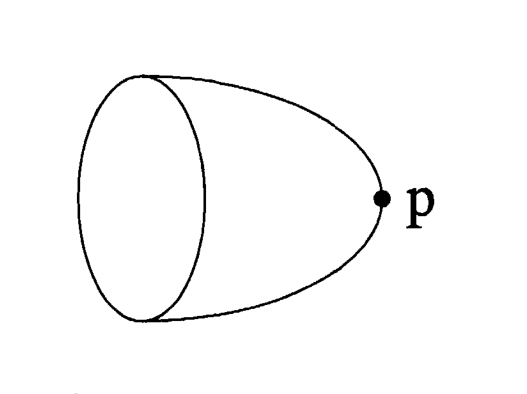
\includegraphics[width=0.40\textwidth]{figs/fig_p202_1.png}
  \caption{带标记点 $p$ 的圆盘（半球）：左侧椭圆表示其边界圆周，$p$ 是内部一点（图中以实心点标出）。在此区域上以给定的边界值作路径积分，便得到从 $p$ 处局域算符到边界场 Hilbert 空间的映射 $\psi$。（原文 Figure 1，p.202）}
  \label{fig:p202-1}
\end{figure}

设 $O$ 是 $p$ 处的一个局域算符。在给定边界值的条件下，对半球上所有场构型作路径积分会给出一个数；当边界值变动时，这个数就成为边界上场的函数。此函数是把边界上的场量子化所得的 Hilbert 空间 $\mathcal H$ 中的一个元素。于是这就给出从 $p$ 处局域算符到 $\mathcal H$ 的一个映射。该映射与 $Q$ 的作用对易，因为路径积分是 $Q$ 不变的；因此它诱导出从局域算符的 $Q$-上同调（即手征环）到圆周上态的 $Q$-上同调 $H^*(Q)$ 的一个映射：
\[
  \psi:(\text{手征环})\longrightarrow H^*(Q).
\]

若 $\mathcal H$ 上 $Q$ 的谱（至少在零点附近）是离散的，则 $\psi$ 是同构。

若 $J_L$ 与 $J_R$ 经典地都是 $R$ 对称性，则手征环与 $\ker H$ 都被这两个对称性赋予双分级（bigrading）。在扭曲理论中，通常分级会出现反常（anomaly），其大小正比于 Riemann 面的 Euler 示性数（对半球而言等于 $1$）。在这种情况下，映射 $\psi$ 把双分级平移
\[
  \psi:H^{p,q}(Q)\longrightarrow \ker H^{p\pm k,\,q\pm k},
\]
其中 $k$ 是反常大小的一个度量。（符号取决于我们所选的是四种扭曲理论中的哪一种。）注意双分级未必按整数分级，而只按有理数分级；这些有理数的分母整除真正作用于理论之上的那个 $U(1)\times U(1)$ 的覆盖的阶。

% [Tutor Note: 此处的 ``$\ker H$'' 指 Hamilton 量 $H$ 的核，而不是「某个映射 $H$ 的核」。在扭曲理论中 $Q$ 是 BRST 型算符，且 $H=\{Q,Q^\dagger\}$，故 $\ker H\subset\ker Q$，而 Hodge 理论给出分解 $\ker Q=\ker H\oplus\operatorname{im}Q$；于是 $\ker H$ 恰是 $Q$-上同调 $H^*(Q)$ 的调和代表空间。作者之所以把两者当成同一对象、并在 $\ker H^{p\pm k,q\pm k}$ 上直接继承双分级，正是用了这一等同。若把它误读成 $H^*(Q)$ 之外的另一个空间，p.204 脚注 2 中「取 $\chi=1$ 时该反常正好产生 §14.3 末尾所说的双分级平移」这句话就无法对上。另需注意：平移量 $k$ 与 $\chi(\Sigma)$ 成正比，而 $\chi(\text{半球})=1$，所以这个例子只是把 $k$ 定标到 $\chi=1$；p.204 的规范理论例子会给出 $k$ 正比于 $\dim G$（而不是每个场贡献 $1$），这才是核对符号与量纲的现成判据。]

\subsection{一个规范理论的例子}
% 原文 §14.4：A Gauge Theory Example

我们取的第一个例子是简单 Lie 群 $G$ 的规范理论。我们从四维的 $\mathcal N=1$ 超对称规范理论出发，做维数约化（dimensional reduction），得到二维的 $\mathcal N=2$ 超对称理论。正如我们在「超习题」（Superhomework）中所见，基本的场强（field strength）是场
\[
  \Sigma=\{\overline{\mathcal D}_+,\mathcal D_-\},
\]
它是取值于主丛（principal bundle）的伴随丛（adjoint bundle）的扭曲手征超场（twisted chiral superfield）。我们使用展开
\[
  \Sigma=\sigma+\cdots+\bar\theta^+\theta^-(F+iD).
\]

% ===== 原文 p.203 =====

玻色场是联络 $A_\mu$ 以及 $\sigma,\bar\sigma$。回忆四维空间上的联络为
\[
  A^{(4)}=\sum_{\mu=0}^{1}A_\mu\,dy^\mu+\sigma(dy^2-i\,dy^3)+\bar\sigma(dy^2+i\,dy^3).
\]
两个 $R$ 对称性是
\[
  J_A=J_L-J_R;\qquad J_V=J_L+J_R.
\]
前者由 $(y^2,y^3)$ 平面内的转动诱导，后者来自四维中的手征 $U(1)$ $R$ 对称性。（该对称性在四维中是反常的，但在二维中不反常——见「超习题」。）现在我们按 $J_V$ 做扭曲，于是 $SO(2)'_E$ 由 $K'=K\pm\tfrac12J_V$ 生成。此时 $A_\mu$ 仍是联络 1-形式，而 $\sigma,\bar\sigma$ 成为 0-形式。一般说来，这种扭曲消去了自旋丛（spin bundle），并把自旋丛的截面变成微分形式。于是四个旋量场 $\lambda_\pm,\bar\lambda_\pm$ 被扭曲成一个 0-形式 $\eta=\psi_{(0)}$、一个 1-形式 $\psi=\psi_{(1)}$ 和一个 2-形式 $\chi=\psi_{(2)}$。（这个新理论当然是存在于紧致曲面上的拓扑理论。它并不具备物理模型所要求的全部通常性质！）

在本例中，$J_A$ 是 $(y^2,y^3)$ 空间转动的两倍，其归一化使得 $[J_A,Q]=Q$。Lagrange 量中各传播场（propagating field）的 $J_A$ 次数如下（参看 [I-Supersolutions, §9.2] 末尾）。（提到「传播场」，意思是我们要用运动方程把辅助场 $F+iD$ 表示为其余场的某个表达式；$F$ 被取为 $A$ 的曲率，$D$ 被取为零，因为理论中没有物质场。）

\begin{center}
\begin{tabular}{|c|c|c|c|c|c|}
\hline
$J_A$-degree & $-2$ & $-1$ & $0$ & $1$ & $2$\\
\hline
field & $\bar\sigma$ & $\psi_{(0)},\psi_{(2)}$ & $A_\mu$ & $\psi_{(1)}$ & $\sigma$\\
\hline
\end{tabular}
\end{center}

% [Tutor Note: 这张表最容易出错之处，是把它读成「形式次数」表。$\sigma$ 与 $\bar\sigma$ 都是 0-形式，$J_A$ 次数却分别是 $+2$ 与 $-2$；而 0-形式的 $\eta=\psi_{(0)}$ 与 2-形式的 $\chi=\psi_{(2)}$ 反而都取 $-1$。正确的读法是「$R$ 荷」表：$\sigma$ 是扭曲手征超场的最高分量以外的标量，带 $R$ 荷 $2$；$\psi_{(k)}$ 的 $J_A$ 次数随形式次数 $k$ 递增。一个立刻可做的自洽性检验是用 p.204 的变换律要求 $\delta$ 把 $J_A$ 次数统一抬高 $1$：由 $\delta\bar\sigma=\psi_{(0)}$ 得 $\deg\bar\sigma=-2$，由 $\delta\psi_{(2)}=F_A$ 得 $\deg F_A=0$，由 $\delta\psi_{(1)}=-D_A\sigma$ 得 $\deg\sigma=+2$（因 $D_A$ 不带 $R$ 荷），由 $\delta\psi_{(0)}=[\sigma,\bar\sigma]$ 得 $2+(-2)=0$，六条式子全部对得上。若谁按「标量都该是 $0$ 次」去记，符号会整体错乱。]

实际上，$J_A$ 的符号可以反过来，但按其中一种选择，次数就如上表所示。

回忆第 11 讲 §11.1：超对称 $Q$ 可以提升为超联络（superconnection）空间上的一个超对称 $\delta$\footnote{在那一讲里我们用的是实场 $\phi$，而这里是复场 $\sigma$，但这不改变任何东西。}。并不是 $\delta^2=0$，而只是 $\delta^2$ 为一个规范变换。事实上 $\delta^2=[\sigma,\cdot\,]$。用坐标场写出，它由下式给出：
\[
\begin{aligned}
  \delta A&=\psi_{(1)},\\
  \delta\psi_{(1)}&=-D_A\sigma,\\
  \delta\sigma&=0.
\end{aligned}
\]
符号 $D_A$ 当然是指关于联络 $A$ 的协变导数。

在第 11 讲 §11.2 中，使用类似的对称性把我们引向联络模空间的等变上同调（equivariant cohomology），经由形式的「标准模型」（the standard model of forms）。设 $\mathcal G$ 是规范群 $G$ 的 Lie 代数，$M$ 是该群作用其上的空间。于是我们有复形
\[
  \bigl(\Omega^*(M)\otimes\operatorname{Func}(\mathcal G)\bigr)^G
\]
其微分是
\[
  D=d_M+i_{V(\phi)}.
\]

% [Tutor Note: 这里写的其实是等变上同调的 \emph{Cartan 模型}：$\operatorname{Func}(\mathcal G)=S(\mathcal G^*)$ 取为 $\mathcal G$ 上的多项式函数，微分 $D=d_M+i_{V(\phi)}$ 中 $i_{V(\phi)}$ 是沿「由 $\phi\in\mathcal G$ 生成的无穷小作用」的内乘。作者称它「经由形式的『标准模型』」，指的是等变上同调的 Weil 模型 $\bigl(\Omega^*(M)\otimes W(\mathcal G)\bigr)^G$（$W(\mathcal G)$ 为 Weil 代数）；两个模型由 Mathai--Quillen 同构等同，细节见 Berline--Getzler--Vergne《Heat Kernels and Dirac Operators》中关于等变上同调的一章。检验 $D^2=0$ 时务必注意 $i_{V(\phi)}^2=0$ 与 $\{d_M,i_{V(\phi)}\}=\mathcal L_{V(\phi)}$（沿作用的 Lie 导数）这两条：$\mathcal L_{V(\phi)}$ 在 $G$ 不变子空间上为零，这才是 $D$ 成为微分的真正原因，作者未加说明。另外，$\delta^2=[\sigma,\cdot\,]$ 而非零，正说明这里的「超对称」只在模掉规范变换的意义下平方为零——这与后面把 $\delta$ 当作等变微分、把 $\sigma$ 当作等变参数是同一件事。]

% ===== 原文 p.204 =====

这一点在第 11 讲中是用手工办法找到的。在我们目前的进路中，从 $\mathcal N=2$ 超对称出发再做扭曲，会遇到另一个与之密切相关的等变上同调模型；它不那么广为人知，但或许本应广为人知。我们把 Lie 代数 $\mathcal G$ 换成它的复化 $\mathcal G_{\mathbb C}$，并构造复形
\[
  \bigl(\Omega^*(M)\otimes\Omega^{0,*}(\mathcal G_{\mathbb C})\bigr)^G.
\]
这里 $\mathcal G_{\mathbb C}$ 上的复线性函数 $\phi$ 的次数为 $2$，函数 $\bar\phi$ 的次数为 $-2$，而 $(0,1)$-形式 $d\bar\phi$ 的次数为 $-1$。此复形中的微分是
\[
  \widetilde D=d_M+i_{\widetilde V(\phi)}+\bar\partial_{\mathcal G_{\mathbb C}},
\]
其中 $\widetilde V$ 是 $M\times\mathcal G_{\mathbb C}$ 上给出该作用的向量场。为看出这个复形同样计算等变上同调，我们把 $\widetilde D$ 看成 $(d_M+i_{\widetilde V(\phi)})$ 与 $\bar\partial_{\mathcal G_{\mathbb C}}$ 之和。我们对这个双复形（double complex）施用通常的谱序列（spectral sequence），先做 $\bar\partial_{\mathcal G_{\mathbb C}}$。由于这个上同调除 $0$ 次以外都为零，而在 $0$ 次处它给出 $\mathcal G_{\mathbb C}$ 上的多项式函数，所以我们看到：得到的结果与第一个复形相同。（注意，这第二种进路给出等变上同调的 Hodge 理论版本，把算子 $\widetilde D^*\widetilde D$ 当作「Laplacian」；理解由此得到的等变上同调的 $L^2$ 版本会是很有意思的。）

% [Tutor Note: 「先做 $\bar\partial_{\mathcal G_{\mathbb C}}$」这一步省掉了谱序列的全部论证。完整的说法是：双复形的 Grothendieck 谱序列以 $E_1^{p,q}=\Omega^{p}(M)\otimes\Omega^{0,q}(\mathcal G_{\mathbb C})$ 出发，$E_2^{p,q}=H^p\bigl(M;\mathcal H^q_{\bar\partial}(\mathcal G_{\mathbb C})\bigr)$。关键事实是 $\mathcal G_{\mathbb C}\cong\mathbb C^n$ 是 Stein（仿射）流形，由 Cartan 定理 B，$q>0$ 时 $H^{0,q}_{\bar\partial}(\mathcal G_{\mathbb C})=0$，而 $q=0$ 时全纯函数就是多项式（因 $\mathcal G_{\mathbb C}$ 复仿射）。于是谱序列在 $E_2$ 处退化，只剩 $\bigl(\Omega^*(M)\otimes\operatorname{Func}(\mathcal G_{\mathbb C})\bigr)^G$，即回到前一复形。作者写「由于这个上同调除 $0$ 次以外都为零」正是引用 Cartan 定理 B，而这一步对紧致复流形会失败（那时 $H^{0,q}$ 一般非零，两个模型不再一致）。另注意 $d\bar\phi$ 的次数取 $-1$ 而非 $+1$，这是为了与 $\bar\partial$ 的次数 $+1$ 相配、使 $\widetilde D$ 齐次；若把 $d\bar\phi$ 记成 $+1$，$\widetilde D^2=0$ 就会被破坏。]

让我们把描述超对称 $\delta$ 在传播场空间上作用的那张表补全。上面这个等变上同调模型翻译成如下超对称变换公式：
\[
\begin{aligned}
  \delta A&=\psi_{(1)},\\
  \delta\psi_{(1)}&=-D_A\sigma,\\
  \delta\sigma&=0,\\
  \delta\bar\sigma&=\psi_{(0)},\\
  \delta\psi_{(0)}&=[\sigma,\bar\sigma],\\
  \delta\psi_{(2)}&=F_A.
\end{aligned}
\]
由最后一式可知，$\delta$ 的不动点将是联络为平坦的场构型；由其余各式可知，截面 $\sigma$ 协变常定（covariantly constant）且与 $\bar\sigma$ 对易。其次我们看到，扭曲之后、在亏格为 $g$ 的 Riemann 面上工作时，$J_A$ 的反常为 $\dim(G)\cdot(-\chi(\Sigma))=-\chi(\Sigma)\cdot\dim(G)$。\footnote{取 $\chi=1$ 时，这个反常正好产生 §14.3 末尾所提到的、从算符到态的映射在双分级上的平移。} 其理由是：路径积分测度中对反常有贡献的项是 $\mathcal D\psi_{(0)}\mathcal D\psi_{(1)}\mathcal D\psi_{(2)}$。Lagrange 量的对称性 $J_A$ 在 $\psi_{(0)}$ 与 $\psi_{(2)}$ 上作用为 $-1$，在 $\psi_{(1)}$ 上作用为 $+1$。因此，关于反常的指标计算变成伴随表示的维数乘以 $-\chi(\Sigma)$。由不变性我们得到
\[
  \Bigl\langle\prod_{\alpha}\int_{\Sigma_\alpha}\mathcal O_\alpha^{(k_\alpha)}\Bigr\rangle=0
\]
除非 $\sum_\alpha n_\alpha=(2g-2)\dim(G)$，其中 $n_\alpha$ 是 $\mathcal O_\alpha^{(k_\alpha)}$ 的 $J_A$ 次数。让我们考虑形如 $P(\sigma)$ 的局域算符，其中 $P$ 是 $G$ 的 Lie 代数上的某个规范不变多项式。这些算符上的环结构正是不变多项式上通常的环结构。容易看出，若 $P$ 的次数为 $r$，则算符 $\mathcal O_P^{(0)}$ 的 $J_A$ 次数为 $2r$，而后代算符（descendant）$\mathcal O_P^{(k)}$ 的 $J_A$ 次数等于 % 接 p.205

% [Tutor Note: 这里的指标约定是核对一切的支点，务必记牢：$\chi(\Sigma)=2-2g$，故 $-\chi(\Sigma)=2g-2$，选择定则 $\sum_\alpha n_\alpha=(2g-2)\dim(G)$ 对球面（$g=0$）给出 $-2\dim(G)$，负号并不奇怪——它只是说总 $J_A$ 次数必须恰好抵消测度带来的反常荷。特别要防止两种误读：(i) 把反常系数当成「每个场 $1$」，那样会漏掉因子 $\dim(G)$，也就无法与 Donaldson 理论中类的维数对上；(ii) 把 $\chi$ 与 $2g-2$ 混用，导致符号整体反号。此外，$\psi_{(0)},\psi_{(2)}$ 的 $J_A$ 荷为 $-1$、$\psi_{(1)}$ 为 $+1$，三者对每个伴随生成元贡献之和恰为 $-1$，乘上重数 $\dim G$ 与 $\chi$ 即得 $-\chi\dim G$：这可以直接从 p.203 那张 $J_A$ 次数表读出来，无需再做指标计算，是检验本页结论最快的办法。]

% ===== 原文 p.205 =====

$2r-k$。注意这些次数与 Donaldson 理论中类似类的通常维数一致。

现在让我们用不动点理论（fixed point theory）来计算 $\bigl\langle\prod_\alpha\int_{\Sigma_\alpha}\mathcal O_\alpha^{(k_\alpha)}\bigr\rangle$。回忆 Lagrange 量为
\[
  \mathcal L=\frac{1}{4e^2}\int d^2y\,d^4\theta\;\operatorname{Tr}\bar\Sigma\Sigma.
\]
我们将为这个关联函数得到一个理论公式。（利用第 11 讲 §11.6 的结果，可以把这个理论公式算出一个具体的实际公式。）用坐标写出，我们有
\begin{equation}
  \tag{14.2}
  \label{eq:14-2}
  \mathcal L=\frac{1}{4e^2}\int d^2y\Bigl(\operatorname{Tr}F^2+\operatorname{Tr}D\sigma D\bar\sigma+\operatorname{Tr}([\sigma,\bar\sigma]^2)+\cdots\Bigr).
\end{equation}
按不动点定理，我们只需在曲率为零且 $D_A\sigma=[\sigma,\bar\sigma]=0$ 的点上计算。有两种情形。若 $A$ 不可约（irreducible）且 $D_A\sigma=0$，则 $\sigma=0$。这些解给出运动方程经典解模空间中的光滑点；而经典 $\delta$ 不变解模空间的这一部分，恰好是 $\pi_1(\Sigma)\to G$ 的不可约表示的空间。另一种可能是 $A$ 可约（reducible）且 $\sigma\ne0$。这些点给出经典解模空间的奇点。回忆 $\sigma$ 取值于复化伴随丛。由于 $D_A\sigma=0$，$\sigma$ 是协变常定的，因此只需在 $\Sigma$ 的某一点上研究其结构。又因 $\sigma$ 与 $\bar\sigma$ 对易，$\sigma$ 可以被 $G$ 中一个元素对角化（即共轭进 $G$ 的 Lie 代数复化的 Cartan 子代数）。

% [Tutor Note: 「曲率为零且 $D_A\sigma=[\sigma,\bar\sigma]=0$」是压缩写法，意思是 $F_A=0$、$D_A\sigma=0$、$[\sigma,\bar\sigma]=0$ 三个条件同时成立，切勿读成「$D_A\sigma$ 等于 $[\sigma,\bar\sigma]$」。逐条对应到上一页的变换律：$\delta\psi_{(2)}=F_A=0$ 给出平坦性，$\delta\psi_{(1)}=-D_A\sigma=0$ 给出协变常定，$\delta\psi_{(0)}=[\sigma,\bar\sigma]=0$ 给出二者对易——所谓「$\delta$ 的不动点」正是把上页六条变换律中涉及费米子的那三条变分置零，然后在规范群作用下取商。另外「$A$ 不可约且 $D_A\sigma=0$ 则 $\sigma=0$」是 Schur 引理的直接推论：$D_A\sigma=0$ 意味着 $\sigma$（伴随丛的截面）在单值群 $\pi_1(\Sigma)$ 的像作用下不变，而不可约性使该表示的中心化子只有标量，伴随表示中不存在非零标量，故 $\sigma=0$。反之 $A$ 可约时中心化子变大，$\sigma$ 才可能取非零值并于 $\Sigma$ 上常定——这正是作者随后把可约联络单列一类的原因。]

现在让我们考察微扰论将如何计算这些拓扑关联函数。我们将限于 $\sigma=0$ 的光滑情形。当然，我们把 Lagrange 量 (14.2) 中的耦合常数 $e$ 取得很小。于是问题化归为在经典解的模空间上（以「超意义」理解）作一个积分。让我们考虑在平坦联络的通常模空间上一点 $[\rho]$ 处把奇变量积掉。费米子空间是 $\psi_{(k)}$ 的零模空间。这些空间是调和形式的空间，因而等同于空间 $H^k(\Sigma,\operatorname{ad}(\rho))$。由于我们假定 $\rho$ 不可约、且模空间在 $[\rho]$ 处光滑，我们有 $H^0(\Sigma,\operatorname{ad}(\rho))=H^2(\Sigma,\operatorname{ad}(\rho))=0$，而 $H^1(\Sigma,\operatorname{ad}(\rho))$ 是模空间在 $[\rho]$ 处的切空间。所以事实上 $[\rho]$ 处的奇方向空间等同于 $\Pi TM_{[\rho]}$。于是，在不可约联络的开子集上，经典解的超流形就是 $\Pi TM$，即平坦联络模空间上奇偶反转的切丛（parity reversed tangent bundle）。正如我们在 [I-Homework] 的问题 FP8 中所见，这样一个超流形的 Berezinian 是自然平凡化的，因此可以在该超流形上对函数作积分。我们也已看到，此超流形上的一个函数等同于 $\mathcal M$ 上的一个微分形式，而在 $\Pi TM$ 上对一个函数作积分等同于在 $\mathcal M$ 上对相应的微分形式作积分。（这需要 $\mathcal M$ 的一个定向，而它由 $\Sigma$ 的一个定向确定。）

当然，我们希望计算涉及算符 $\int_{\Sigma_\alpha}\mathcal O_\alpha^{(k_\alpha)}$ 的关联函数。这些算符确定了 $\Pi TM$ 上的函数，而它们之积的关联函数就变成这些函数之积的积分。按这种方式，$\sigma$ 的规范不变多项式被映为 $\Pi TM$ 上的函数，从而被映为 $\mathcal M$ 上的微分形式。从多项式约化到微分形式的关键一步，是如下观察：当存在费米子时，已经不 % 接 p.206

% ===== 原文 p.206 =====

再是 $\sigma=0$ 的情形了。相反，运动方程给出
\[
  \Box\sigma=-[\psi_{(1)},\psi_{(1)}].
\]
这一点很重要，因为右端可以直接解释为模空间上的一个 2-形式（$\psi_{(1)}$ 的零模表示模空间上的 1-形式），所以这个公式使我们能用模空间上一个通常的 2-形式来表达函数 $\sigma$——在量子场论的形式体系中，$\sigma$ 形式上次数为二。人们通过把这样得到的微分形式在模空间上积分来计算关联函数。（当然，这些计算还必须在由可约联络以及非零但平行的场 $\sigma$ 给出的那些分支上补充相应的计算。）

在这个规范理论例子中，由于可约联络的存在，Hamilton 量具有从零能量开始的连续谱。结果，从算符的 $Q$-上同调到态的 $Q$-上同调的那个映射就不太有用。

% [Tutor Note: $\Box$ 在此指规范协变的 Laplacian $D_A^*D_A$（$\Sigma$ 上的），而 $\psi_{(1)}$ 是 1-形式取值的费米子，故 $[\psi_{(1)},\psi_{(1)}]$ 是 2-形式取值的（Lie 代数伴随）场——作者紧接着说的「右端可直接解释为模空间上的 2-形式」正是基于这一点：$\psi_{(1)}$ 的零模是模空间的 1-形式，两个 1-形式缩并便得到 2-形式。这里有三个易错点：(i) 负号依赖于 $\Box=D_A^*D_A$ 的符号约定与费米子双线性型的约定，改用 $\Box=-D_A^*D_A$ 会把负号翻掉；(ii) 括号是 Lie 代数括号与形式楔积的组合 $[\psi_{(1)},\psi_{(1)}]^a=f^a{}_{bc}\,\psi_{(1)}^b\wedge\psi_{(1)}^c$（$f^a{}_{bc}$ 为结构常数），切勿误写成 $\psi_{(1)}\wedge\bar\psi_{(1)}$；(iii) 正因为 $\sigma$ 的期望值被费米子双线性型「撑起来」，$\sigma$ 才不能简单地被置零，这也是为什么前面 $\sigma=0$ 的微扰计算必须在此处被修正。顺带说明本页最后一句与前文 p.202 的呼应：那里的同构 $\psi$ 要求 $Q$ 的谱在零点附近离散，而可约联络造成的连续谱恰好破坏了这一前提，这正是规范理论例子中该映射「不太有用」的原因。]

\subsection{一个 $\sigma$ 模型的例子}
% 原文 §14.5：A $\sigma$-model example

让我们考虑 $\mathcal N=2$ 超对称 $\sigma$ 模型
\[
  \Phi:\Sigma\longrightarrow X,
\]
其中 $X$ 是 Kähler 流形，而 $\Sigma$ 是如上一个规范理论例子中那样的分裂 $2|4$ 流形。在这一假定下，$\sigma$ 模型的费米子位于
\[
  K_\Sigma^{\pm1/2}\otimes T^{\pm}X,
\]
其中 $K_\Sigma$ 是 $\Sigma$ 的典范丛（canonical bundle），而 $T^+X=T^{1,0}X$ 与 $T^-X=T^{0,1}X$ 是 $X$ 的全纯与反全纯切丛。我们把这些费米子记作 $\chi^{\pm,\pm}$。第一个符号指该费米子是左行还是右行（即它是 $K_\Sigma^+$ 还是 $K_\Sigma^-$ 的截面），第二个符号指它在 $X$ 上的截面类型（全纯或反全纯）。为使理论在 $\Sigma$ 上有整体定义，我们再一次扭曲理论，把 $K$ 换成
\[
  K'=K\pm\tfrac12J_L\pm\tfrac12J_R.
\]
此时有些费米子是 $T^{\pm}X$ 的截面，另一些则是 $K_\Sigma^{\pm1}\otimes T^{\pm}X$ 的截面。取决于扭曲中符号的选择，我们得到两种可能的理论，分别称为 $A$ 模型（用 $-\tfrac12J_L+\tfrac12J_R$）与 $B$ 模型（用 $\tfrac12J_L+\tfrac12J_R$）。

\subsubsection{$A$ 模型}
% 原文 §14.5.1：The $A$-model

扭曲后在 $\Sigma$ 上作为 0-形式变换的费米子是 $\chi^{++}\in T^{1,0}X$ 与 $\chi^{--}\in T^{0,1}X$。0-形式算符之环的一般元素是
\[
  F(\Phi,\chi^{++},\chi^{--}).
\]
这些算符构成的环是 $\Pi TX$ 上函数之环，而后者等同于 Kähler 流形上微分形式之环。进一步，在用相应的算符 $\mathcal O_F$ 来标识微分形式 $F$ 之后，我们有
\[
  Q\mathcal O_F=\mathcal O_{dF},
\]
于是 $Q$ 成为通常的外微分。手征环于是就是 $H^*(X)$，即 $X$ 的通常拓扑上同调；而由 $J_L$ 与 $J_R$ 诱导的双分级 % 接 p.207

% ===== 原文 p.207 =====

就是通常的 Hodge 双分级。在映射空间中，$Q$ 的不动点是全纯曲线
\[
  \phi:\Sigma\longrightarrow X.
\]
（要看出这一点，必须考察那些在扭曲模型中作为 $\Sigma$ 上 $(1,0)$-形式或 $(0,1)$-形式变换的费米子的超对称变换律。）因此，要在此模型中计算关联函数，我们必须对 $X$ 中全纯曲线的空间作积分。如我们将在下一讲看到的，这将引向量子上同调（quantum cohomology）。

\subsubsection{$B$ 模型}
% 原文 §14.5.2：The $B$-model

只有在 $X$ 为 Calabi--Yau 的情形才能构造这个模型，因为只有在这种情形下，我们想用来扭曲的对称性 $(J_L+J_R)$ 才不反常\footnote{换言之，若 $c_1(X)$ 非零，则 $J_L+J_R$ 甚至在做规范化（gauging，指与二维引力耦合）之前就已经不是量子理论的对称性了。本讲第一部分关于「做规范化的障碍」的讨论假定了 $J_L$ 与 $J_R$ 在规范化之前都生成对称性，因此不适用于这一情形。}。我们在 $X$ 上固定一个非零的全纯 $n$-形式 $\omega$。在此情形下 0-形式是 $\chi^{+-}\in T^{1,0}X$ 与 $\chi^{-+}\in T^{0,1}X$。0-形式算符之环是
\[
  F(\Phi,\chi^{+-},\chi^{-+}),
\]
也就是环
\[
  \Omega^{0,*}(X)\otimes\Omega^{0,*}(X)=\Omega^{0,*}\bigl(X,\wedge^*T^{1,0}X\bigr).
\]
在这一标识下我们有
\[
  Q\mathcal O_F=\mathcal O_{\bar\partial F},
\]
于是手征环是
\[
  \bigoplus_{q,p}H^q\bigl(X;\wedge^pT^{1,0}X\bigr).
\]
场空间中的 $Q$ 不动点是常映射 $\Sigma\to X$。因此，此模型中关联函数的计算将成为 $X$ 上的积分
\[
  \Bigl\langle\prod_{i=1}^{s}\mathcal O_{F_i}\Bigr\rangle=\int_X\bigl(\wedge_{i=1}^{s}F_i\bigr)\cdot\omega^{\otimes2}.
\]
这些积分稳稳地属于经典数学；它们与复结构形变下 Hodge 结构的变分（variations of Hodge structure）有关。

% [Tutor Note: 两个模型的存在条件差别极大，此处最易记错。$A$ 模型用 $-\tfrac12J_L+\tfrac12J_R$ 扭曲，反常正比于 $c_1(X)$ 的两个贡献符号相反，恰相消，故任何 Kähler 流形都可定义 $A$ 模型（这也解释了为什么 $A$ 模型只需 $X$ Kähler）；$B$ 模型用 $+\tfrac12J_L+\tfrac12J_R$，两个贡献同号相加，反常量正比于 $2c_1(X)$，故必须 $c_1(X)=0$，即 $X$ Calabi--Yau——这正是脚注 3 所说的「否则 $J_L+J_R$ 连对称性都不是」。另需注意末式中的 $\omega^{\otimes2}$ 是与 $\wedge_{i=1}^s F_i$ 配对的测度：Calabi--Yau 上的自然体积形式是 $\omega\wedge\bar\omega$（一个 $(n,n)$-形式），作者写 $\omega^{\otimes2}$ 是把它当作「$|\omega|^2$」的简写；若字面理解为两个 $(n,0)$-形式的张量积而不取共轭，则结果不是实量，配对也无法进行。最后，$\bar\partial$ 与 $d$ 的区别正是 $A/B$ 模型的分水岭：$A$ 模型的 $Q$ 是外微分 $d$（手征环 $=H^*(X)$，逐次上同调），$B$ 模型的 $Q$ 是 $\bar\partial$（手征环 $=\oplus_{p,q}H^q(X;\wedge^pT^{1,0}X)$，即 Hodge 分次），两者绝不能互换。]

\subsection*{参考文献与交叉引用}

关于本讲的许多材料，一个参考文献是

\begin{quote}
E.~Witten, \emph{Mirror Manifolds And Topological Field Theory}, in \emph{Essays on mirror manifolds}, 120--158, Internat.\ Press, Hong Kong, 1992.
\end{quote}

这里的许多材料与第 11 讲的内容密切相关。由 $\Pi TM$ 构造的超流形的 Berezinian 的平凡化，以及该超流形上函数与微分形式的等同，也见于 [I-Dirac Index, §1.2]。关于 $R$ 对称性的基本材料见于 [I-Supersolutions] 第 9 章。能量动量张量与度规变分的关系在 [I-Classical Fields, §2.9] 中有解释，并在共形场论的语境下于 [II-CFT, §2.1] 与 [II-Strings, §2.1] 中作了描述。拓扑扭曲量子场论中拓扑关联函数的两个例子，在这些讲末尾的问题 10 与问题 11 中作了详细计算。

% [Tutor Note: 引文中的 [I-Dirac Index]、[I-Supersolutions]、[I-Classical Fields]、[II-CFT]、[II-Strings] 均是本丛书（\emph{Quantum Fields and Strings: A Course for Mathematicians}）第 I、II 卷对应章节的代号，作者以此代替具体页码；其中 [I-Dirac Index] 讲 Dirac 算符与指标定理，[II-CFT] 与 [II-Strings] 分别是第 II 卷的共形场论与弦论部分。原文此处把 Berezinian 的平凡化归于 [I-Dirac Index, §1.2]，而正文 p.205 却把它归于 [I-Homework] 的问题 FP8，两处指向不同，阅读时不必视为矛盾——前者是系统讲述，后者是习题中的具体算例。另：所谓「问题 10 与问题 11」指本讲系列末尾（全书习题部分）的两个练习，与 p.205 关于 $\Pi TM$ 上积分等于 $\mathcal M$ 上微分形式积分的论述互为补充。]


\clearpage
% 原文 pp.209–215（印刷 pp.1327–1333）
\section{Lecture 15：$\mathcal{N}=2$ 极小模型的 Landau–Ginzburg 描述与 Kähler 流形的量子上同调}

\begin{keytakeaways}
本讲前半部分系统整理了「某些 Landau--Ginzburg 模型的红外极限等于代数上可构造的 $\mathcal{N}=2$ 极小模型（minimal model）」这一断言的已有证据。物理图像是：超势的拟齐次性（quasi-homogeneity）给出一个可以延拓到超荷上的 $R$ 对称性，它的手征反常系数 $k$ 是拓扑不变量，可在紫外自由场论中精确算出，而它恰等于红外极限共形场论的中心荷 $\widehat{c}$。核心数学工具是 $\mathcal{N}=2$ 超共形代数的表示论、$\overline{Q}_+$（等价地 $\overline{D}_+$）上同调，以及椭圆亏格（elliptic genus）的路径积分与特征标两种算法。主要结论是 $\widehat{c}=\sum_j(1-2\alpha_j)$ 这一对各个手征超场逐项求和的公式，它把 Landau--Ginzburg 轨形、非线性 $\sigma$ 模型与加权射影空间中的 Calabi--Yau 超曲面串成同一条 UV--IR 链条。本讲末尾把这一图像接到加权射影空间与 Calabi--Yau 超曲面上，为后续的量子上同调（quantum cohomology）讨论作准备。
\end{keytakeaways}

% ===== 原文 p.209 =====

\subsection{Landau--Ginzburg 模型}
% 原文 §15.1：Landau-Ginzburg models

今天这讲前半部分的主题，是更详细地讨论一个已有断言所依据的已知证据：某些 Landau--Ginzburg 模型的红外（IR）极限，与那些代数上可构造的、被称为「极小模型」（minimal model）的共形场论（conformal field theory，CFT）等价。

先考虑最简单的 Landau--Ginzburg 模型：一个含单个手征超场（chiral superfield）$\Phi$ 的二维 $\mathcal{N}=2$ 理论，其拉氏量为
\[
  \mathcal{L}=\int d^2x\,d^4\theta\;\overline{\Phi}\Phi
  +\left(\int d^2x\,d\theta^+\,d\theta^-\,\Phi^k+{\rm c.c.}\right).
\]

我们在第 13 讲 §13.6.1 中的断言是：该模型在红外流向一个中心荷（central charge）为 $\widehat{c}=1-\frac{2}{k}$ 的共形场论。若此说成立，则它所流向的理论是代数可解的，因为中心荷 $\widehat{c}<1$ 的 $\mathcal{N}=2$ 超共形代数（superconformal algebra）的表示已有已知的分类。更确切地说，固定 $\widehat{c}=1-\frac{2}{k}$ 之后，该中心荷的代数的不可约表示 $\mathcal{H}_\alpha$ 只有有限多个（在同构意义下）。中心荷为 $\widehat{c}=1-\frac{2}{k}$ 的共形场论由其 Hilbert 空间完全确定，而这些 Hilbert 空间是由上述表示的张量积之和
\[
  \bigoplus_{\alpha,\beta}\left(\mathcal{H}_\alpha\otimes\overline{\mathcal{H}}_\beta\right)^{e_{\alpha\beta}}
\]
配以一个模不变（modular invariant）的特征标（character）构造出来的。这类组合有一个 $A$-$D$-$E$ 分类。其中最简单的模不变组合——也正是这里将会出现的那个——是对所有表示取无权对角和：
\[
  \bigoplus_{\alpha}\mathcal{H}_\alpha\otimes\overline{\mathcal{H}}_\alpha .
\]
（这对应于 $A$ 系列。）

更一般的 Landau--Ginzburg 模型含有若干个手征超场 $\Phi_1,\dots,\Phi_n$，以及一个拟齐次多项式（quasi-homogeneous polynomial）$W(\Phi_1,\dots,\Phi_n)$，它充当理论的超势（superpotential）。我们应当假定该多项式是横截的（transverse），

\noindent\textit{（本讲笔记整理者：John Morgan 与 David Morrison。）}

% ===== 原文 p.210 =====

其含义是 $W=dW=0$ 只在原点成立；而拟齐次性条件则可以表述为：存在正有理数 $\alpha_j$，使得
\[
  W=\sum_j\alpha_j\Phi_j\frac{\partial W}{\partial\Phi_j}.
\]

拉氏量可以写为
\[
  \mathcal{L}=\int d^2x\,d^4\theta\;\overline{\Phi}_j\Phi_j
  +\left(\int d^2x\,d\theta^+\,d\theta^-\,W(\Phi_j)+{\rm c.c.}\right).
\]

直观上，拟齐次性之所以重要，是因为它使得其中一个 $R$ 对称性（$R$-symmetry）有可能延拓为
\[
  \theta^+\to e^{i\varepsilon}\theta^+,\qquad \theta^-\to\theta^-,
\]
并作用在手征场上为 $\Phi_j\to e^{i\varepsilon\alpha_j}\Phi_j$，从而使超势按 $W\to e^{i\varepsilon}W$ 变换，拉氏量因而保持不变。如果我们假定这一微观的 $R$ 对称性在红外成为极限共形场论的左移 $R$ 对称性，那么我们就能借助算子乘积展开（operator product expansion，OPE）算出该极限理论的中心荷 $\widehat{c}$。

具体做法如下。回想在第 13 讲中我们遇到过一个常数 $k$，它度量的是：若试图把 $R$ 对称性 $J_L$ 规范化（gauging），会出现多大的反常（anomaly）。这个常数在算子乘积展开中表现为
\[
  J_L(x)J_L(x')=\frac{k}{(x^--x'^-)^2}+\cdots .
\]

把 $k$ 解释为规范化的阻碍，就立刻可以看出它是一个拓扑不变量，因而可以在任何标度下可靠地测量或计算。特别地，它可以在紫外（UV）计算，而在紫外超势无关紧要。（这样，规范化的阻碍是由一个指标问题（index problem）算出来的，无论我们所处的 Riemann 面是大是小都成立；我们可以把它取得足够小，以致超势完全无关。）另一方面，如果 $J_L$ 正是极限 $\mathcal{N}=2$ 超共形场论中出现的那同一个 $R$ 对称性，那么超共形代数的算子乘积展开就断言
\[
  J_L(x)J_L(x')=\frac{\widehat{c}}{(x^--x'^-)^2}+\cdots ,
\]
其中 $\widehat{c}$ 是 $\mathcal{N}=2$ 代数中的中心荷。于是 $k=\widehat{c}$，我们便可以通过在紫外做计算来测出红外的中心荷。

要在紫外计算 $k$，就把各个场当作自由场。规范化的阻碍来自这样一个事实：在自由的超多重态里，$R$ 对称性就是费米子的手征对称性。按照第 6 讲 §6.2 的方法，我们有 $k=\sum b_i^2-\sum c_i^2$，其中 $b_i$ 与 $c_i$ 分别是左手征费米子与右手征费米子的 $R$ 荷。在我们的问题里，$b_i=-1+\alpha_i$、$c_i=\alpha_i$，于是得到 $k=\sum_i(1-2\alpha_i)$。假定红外流向一个 $\mathcal{N}=2$ 理论、且其中出现同一个 $R$ 对称性，就有 $k=\widehat{c}$，从而 $\widehat{c}=\sum_j(1-2\alpha_j)$。注意：在单个场、$W(\Phi)=\Phi^k$ 的情形，必须有 $\alpha=1/k$，于是我们得到所期望的结果 $\widehat{c}=1-2/k$。

% [Tutor Note: 这一步是全讲最容易出错的地方，有两处要当心。其一，$k=\sum b_i^2-\sum c_i^2$ 中的 $b_i,c_i$ 是第 6 讲 §6.2 意义下左、右手征费米子的 $R$ 荷，而同一个手征超场 $\Phi_j$ 的两个费米子分量的荷相差 $1$（差的那个 $1$ 来自 $\int d^2\theta$ 测度、也就是超势的量纲），所以才会有 $b_i=-1+\alpha_i$ 而不是 $b_i=\alpha_i$；一旦漏掉这个 $-1$，就得到 $k=\sum\bigl(\alpha_i^2-\alpha_i^2\bigr)=0$，即"没有反常"，这与 $\widehat{c}=1-2/k$ 直接冲突。其二，是荷的平方差 $b_i^2-c_i^2$ 而不是差的平方 $(b_i-c_i)^2$：反常是荷平方之差的和，误写成一次差会把 $\alpha_i$ 的二阶项全部丢掉。最后，$\alpha=1/k$ 的来历作者没有写：把 $W=\Phi^k$ 代入拟齐次性条件得 $W=\alpha\Phi\,\partial_\Phi W=\alpha k\,\Phi^k$，故 $\alpha k=1$。]

我们现在要给出一个更精细的论证来支持这一等价性，它将揭示（极限）共形场论更多的结构。

% ===== 原文 p.211 =====

回想 $\mathcal{N}=2$ 代数的结构：
\[
  \{Q_\pm,\overline{Q}_\pm\}=P_\pm,\qquad \{Q_\pm,Q_\pm\}=0 .
\]
我们有 $\overline{Q}_+^2=0$，因此可以考察 $\overline{Q}_+$ 的上同调（cohomology），也就是考察那些满足 $\{\overline{Q}_+,\mathcal{O}\}=0$ 的局部算符 $\mathcal{O}=\mathcal{O}(x)$。于是
\[
  \partial_+\mathcal{O}=[\{Q_+,\overline{Q}_+\},\mathcal{O}]
  =[\overline{Q}_+,\{Q_+,\mathcal{O}\}],
\]
也就是说，用欧氏语言（把 $(x^+,x^-)$ 与 $(z,\overline{z})$ 等同起来），$\mathcal{O}(x)$ 在 $\overline{Q}_+$ 上同调中的类是全纯地变化的。

取两个这样的算符，用全纯语言写为
\[
  \mathcal{O}(z)\mathcal{O}'(z')=\sum_k f_k(z-z')\mathcal{O}_k(z')
  +\{\overline{Q}_+,\cdots\},
\]
其中 $f_k$ 是全纯函数。由这个公式可以看出，$\overline{Q}_+$ 上同调具有共形场论的一般结构，其中的算符是「纯左移的」，即它们全纯地变化。

一个重要注记是：$\overline{Q}_+$ 上同调在 Weyl 重标度（Weyl rescaling）下不变，因而它只依赖 Riemann 面的复结构（complex structure），而与度规无关。要看出这一不变性，我们必须证明 $T_{z\overline{z}}$ 是 $\overline{Q}_+$-恰当的（$\overline{Q}_+$-exact）。一个自然的证法是修改关于标度不变性的通常定义：利用多项式的拟齐次性，使得超势项在修改后的标度变换下保持不变。于是作用量中的动能项就不再标度不变，但动能项的改变量具有 $\int d^4\theta(\cdots)$ 的形式（因为动能项本身就有这一性质），从而是 $\overline{Q}_+$-恰当的。

% [Tutor Note: 作者说"一个自然的证法是修改标度不变性的定义"，这句话背后压掉了两小步。(1) 修改后的标度变换之所以能保住超势项，正是因为拟齐次性：给 $\Phi_j$ 赋权 $\alpha_j$、给 $\theta^+$ 赋权 $\frac12$、给 $\theta^-$ 赋权 $0$，$\int d^2\theta\,W$ 的总权才为零；若没有拟齐次性，$W$ 项单独就会被标度变换破坏，"修改定义"根本无从谈起。(2) 得到动能项的变分形如 $\int d^4\theta(\cdots)$ 之后，还要说明这类项在 $\overline{Q}_+$ 上同调中为零——用的正是本页上面那个恒等式：对 $\overline{Q}_+$-闭的算符，$\partial_+$ 作用后等于 $[\overline{Q}_+,\{Q_+,\cdot\}]$，自动落在 $\overline{Q}_+$ 的像里。所以"自然的证法"实质上是：用改进后的（无迹）能动张量把 $T_{z\overline{z}}$ 写成某个局部算符的全导数，再用 $\partial_+\mathcal{O}=[\overline{Q}_+,\{Q_+,\mathcal{O}\}]$ 收尾。]


以上我们用 $\overline{Q}_+$ 上同调来表述，是为了能涵盖非常一般的 $\mathcal{N}=2$ 理论。然而，只要理论有超空间实现（我们正在研究的 Landau--Ginzburg 理论正是如此），更方便的做法就是研究 $\overline{D}_+$ 上同调而非 $\overline{Q}_+$ 上同调，其中
\[
  \overline{D}_+=e^{-\theta^+\overline{\theta}^+\partial_+}\,
  \overline{Q}_+\,e^{\theta^+\overline{\theta}^+\partial_+},
\]
于是 $\overline{D}_+$ 上同调与 $\overline{Q}_+$ 上同调自然同构。

在我们的 Landau--Ginzburg 理论中，运动方程为
\[
  2\overline{D}_+\overline{D}_-\Phi^j=\frac{\partial W}{\partial\Phi^j}.
\]
考虑算符
\[
  \mathcal{T}=\sum_j\left(
  \left(\frac{1-\alpha_j}{2}\right)D_-\Phi^j\;\overline{D}_-\,\overline{\Phi}_j
  -i\alpha_j\,\overline{\Phi}_j\,\partial_-\Phi_j
  \right);
\]
则 $\overline{D}_+\mathcal{T}=0$，于是它定义了一个 $\overline{D}_+$ 上同调类。\footnote{此处本应担心反常，但实际上「$\overline{D}_+\mathcal{T}=0$」这一陈述并没有量子反常；不过在带 $(0,2)$ 超对称的二维模型中，一些颇为相似的陈述确实存在这类反常。参见 E.~Silverstein 与 E.~Witten, ``Global $U(1)$ $R$ Symmetry And Conformal Invariance Of $(0,2)$ Models,'' Phys.\ Lett.\ \textbf{B328} (1994) 307.}

% [Tutor Note: 这个 $\mathcal{T}$ 的指标写法在原书里并不统一，抄写时极易出错：第一项是 $D_-\Phi^j\,\overline{D}_-\,\overline{\Phi}_j$，前一个因子取上标 $j$、后一个取下标 $j$；而末项写成 $-i\alpha_j\overline{\Phi}_j\partial_-\Phi_j$ 时两个都取下标；到了 p.215 的 Kähler 项又写成 $\overline{\Phi}^j\Phi^j$（两个都取上标）。由于 $\Phi_j$ 与 $\overline{\Phi}_j$ 互为复共轭、$\alpha_j$ 为实数，这些写法在数值上等价，但若按"上下标必须成对缩并"的规则去读，会误以为原式有笔误。另外运动方程写成 $2\overline{D}_+\overline{D}_-\Phi^j=\partial W/\partial\Phi^j$，那个因子 $2$ 是约定相关的（取决于 $\overline{D}_\pm$ 的归一化，以及 Kähler 势取 $\overline{\Phi}\Phi$ 还是 $\frac12\overline{\Phi}\Phi$）；要核对 $\mathcal{T}$ 的两个系数 $(1-\alpha_j)/2$ 与 $i\alpha_j$ 是否配对正确，最可靠的办法就是按本页给出的运动方程把 $\overline{D}_+\mathcal{T}$ 实算一遍，并注意 $\overline{D}_+$ 只作用在含 $\overline{\theta}^+$ 的因子上。]

在自由理论中，取 $W=0$，$\mathcal{T}$ 是一个维数为 $(1,0)$ 的算符。如果我们面对的是超共形理论，就能把它写成
\[
  \mathcal{T}=J+\theta^-G+\overline{\theta}^-\,\overline{G}
  +\theta^-\overline{\theta}^-\,T .
\]

% ===== 原文 p.212 =====

如果我们确实在极限处得到一个 $\mathcal{N}=2$ 共形场论，那就应当期望有如下形式的 OPE：
\[
  \mathcal{T}(x)\mathcal{T}(y)=\frac{\widehat{c}}{(x-y)^2}
  +\frac{\mathcal{T}}{(x-y)}+\text{关于 }\mathcal{O}\text{ 全纯的项}.
\]
在自由场论中我们可以验证这一结构：第一项来自形如下图的一个图，其中两个算符之间交换了两条传播子：

\begin{figure}[htbp]
  \centering
  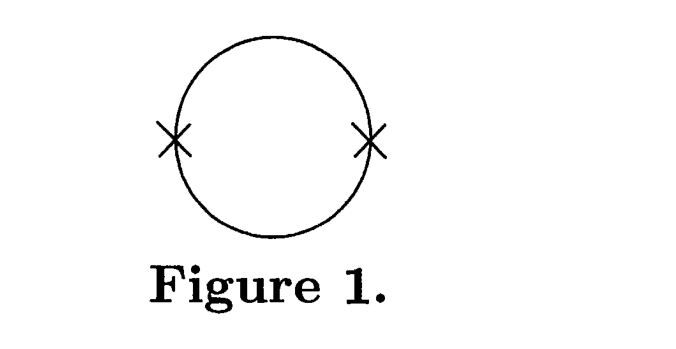
\includegraphics[width=0.30\textwidth]{figs/fig_p212_1.png}
  \caption{第一项所对应的图形：两个算符之间交换两条传播子，构成一个闭合的圈（单圈自收缩图），给出 $1/(x-y)^2$ 型的接触项，其系数即中心荷 $\widehat{c}$。（原文 Figure 1，p.212）}
  \label{fig:p212-1}
\end{figure}

\noindent 而第二项则来自形如下图的一个图，其中只交换了一条传播子：

\begin{figure}[htbp]
  \centering
  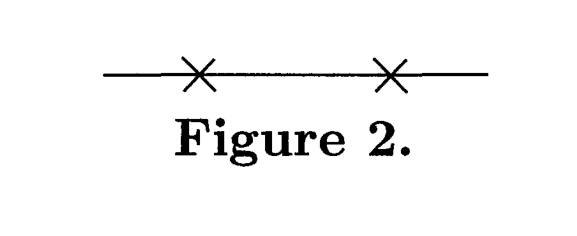
\includegraphics[width=0.26\textwidth]{figs/fig_p212_2.png}
  \caption{第二项所对应的图形：两个算符之间只交换一条传播子，给出 $1/(x-y)$ 型的项，其算符系数即 $\mathcal{T}$ 本身。（原文 Figure 2，p.212）}
  \label{fig:p212-2}
\end{figure}

\noindent 其中只交换了一条传播子。

请注意，在算子乘积展开中计算这些项时，我们可以令 $W=0$，因为超势项太软（too soft，即可超重整化），不会对这些奇异性有贡献。这样做完之后，不同的超场彼此解耦，于是 $\widehat{c}$ 的计算就是各个超场贡献之和。由此立刻得到一个结论：$\widehat{c}$ 对 $\alpha_j$ 是可加的，即 $\widehat{c}=\sum_j f(\alpha_j)$，其中 $f$ 是某个函数。具体计算给出 $f(\alpha)=1-2\alpha$，与我们第一种做法一致。

% [Tutor Note: "超势太软"这句话在二维要按量纲来读：二维中 $\int d^2\theta\,W$ 无量纲、而 $d^2\theta$ 的量纲为 $1$，故 $[W]=1$；于是超势只能产生可去的小动量行为，无法生成 $1/(x-y)^2$ 这种短距离奇异性，因此在算 OPE 奇异项时尽可令 $W=0$。这一点是关键：正因如此不同超场才解耦，$\widehat{c}$ 才对 $\alpha_j$ 可加，$\widehat{c}=\sum_j f(\alpha_j)$ 才成立。顺带提醒，此处加的是 $\widehat{c}=c/3$：若误用 $c$，可加性形式上仍成立但数值差三倍，在 $W=\Phi^k$ 时就会把 $c=3(1-2/k)$ 与 $c=1-2/k$ 混为一谈。至于这两个图，要注意 Figure 1 是"算符—算符"之间的单圈自收缩（两条传播子），不要读成双圈图；Figure 2 才是单传播子交换。]

总之，即使在我们这个微观拉氏量里，也能看到一个算符 $\mathcal{T}$，它在 $\overline{D}_+$ 上同调这一层面上满足 $\mathcal{N}=2$ 超共形代数。因此可以推测：该理论在红外流向一个共形场论，而其 $\overline{D}_+$ 上同调包含该超共形代数。

如果我们只有一个手征超场，从而 $\widehat{c}<1$，那么 $\mathcal{N}=2$ 代数在量子 Hilbert 空间中的作用几乎是不可约的。因此应当期望 $\mathcal{T}$ 会生成 $\overline{Q}_+$ 上同调。对于 $\widehat{c}>1$，$\mathcal{N}=2$ 代数的作用方式远非不可约，要得到一个代数可解的模型就需要额外的生成元。至于某些 Landau--Ginzburg 模型是否真的存在这样的额外生成元，目前尚不清楚（除了超势为若干不同变量的函数之和这一显然情形之外）。

\subsection{椭圆亏格}
% 原文 §15.2：The elliptic genus

我们将通过椭圆亏格（elliptic genus）的计算，给出这些理论之间等价性的更多证据。我们在亏格 $1$ 的 Riemann 面上工作，其周期格由 $1$ 与 $\tau$ 张成。

\begin{figure}[htbp]
  \centering
  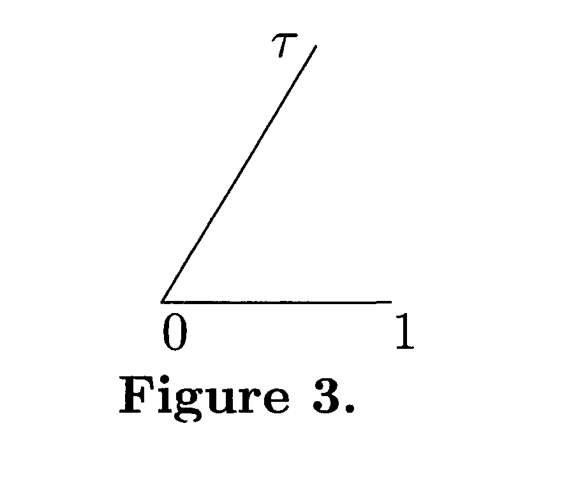
\includegraphics[width=0.34\textwidth]{figs/fig_p212_3.png}
  \caption{亏格 $1$ Riemann 面的周期格：由 $1$ 与 $\tau$ 张成，$\tau$ 取在上半平面。（原文 Figure 3，p.212）}
  \label{fig:p212-3}
\end{figure}

% ===== 原文 p.213 =====

我们令 $q=e^{2\pi i\tau}$，并计算
\[
  \mathrm{Tr}\;q^{(H-P)/2}\,\overline{q}^{(H+P)/2}(-1)^{F_R}.
\]

在环面的空间方向上，我们对左移与右移费米子都取周期边界条件。插入 $(-1)^{F_R}$ 意味着：右移费米子 $\psi_+,\overline{\psi}_+$ 在时间方向上也应当取周期边界条件，从而构成奇（odd）旋量结构（即在两个方向上都周期的那一种）；而左移费米子 $\psi_-,\overline{\psi}_-$ 在时间方向上应当是反周期的，因而它们是偶（even）旋量丛的截面。

\begin{figure}[htbp]
  \centering
  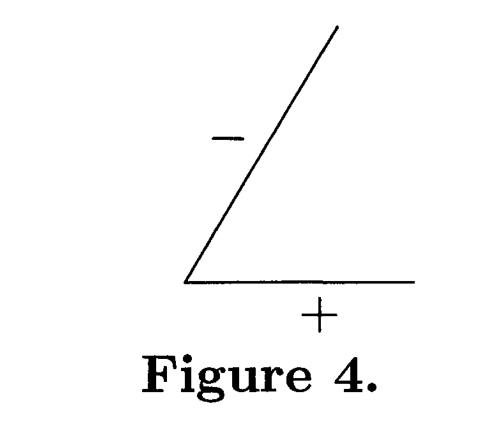
\includegraphics[width=0.26\textwidth]{figs/fig_p213_1.png}
  \caption{环面上两组费米子边界条件的示意：水平边标以「$+$」，斜边标以「$-$」，表示一组费米子在两个方向上都取周期（奇旋量结构）、另一组在时间方向取反周期（偶旋量结构）。（原文 Figure 4，p.213）}
  \label{fig:p213-1}
\end{figure}

% [Tutor Note: 自旋结构这句话最容易记反。按本文的 $\pm$ 约定，$\psi_+$ 是右移、$\psi_-$ 是左移；空间方向两者都取周期（环面上空间方向没有别的选择），时间方向则由 $(-1)^{F_R}$ 的插入决定：$\psi_+$ 在时间方向也周期（两方向皆周期 $=$ 奇旋量结构），$\psi_-$ 在时间方向反周期（偶旋量丛）。若把插入误写成 $(-1)^{F_L}$，两个 $\pm$ 的角色互换，所得函数会变成以 $\overline{q}$ 展开的那一个，与 p.215 的乘积公式对不上。一个现成的自洽性检验是：p.215 的最终结果只含 $q$、不含 $\overline{q}$，这正与 p.214 中"右移部分被 $(-1)^{F_R}$ 投影到基态、只剩 $1$ 或 $0$"相吻合。]

带这些边界条件的路径积分只需 $\mathcal{N}=1$ 超对称就能引入；而且正如我们去年秋天讨论过的，单在这一背景下它就已经相当有趣。它可以被解释为 $\mathcal{N}=1$ 理论右移超荷的指标（index）。

在 $\mathcal{N}=2$ 超对称的情形，故事更有意思，因为还有进一步丰富的余地：可以在迹中插入 $e^{i\gamma J_L}$，它与 $Q_+$ 和 $\overline{Q}_+$ 都对易，因而保持了「指标」这一解释。\footnote{我们对左 $R$ 流以及由它导出的守恒荷使用同一个符号 $J_L$。}我们考虑函数
\[
  F(q,\gamma)=\mathrm{Tr}\;q^{(H-P)/2}\,\overline{q}^{(H+P)/2}\,
  e^{i\gamma J_L}(-1)^{F_R}.
\]

为了用路径积分表示这个迹，我们按惯例把一个柱面的两端粘起来，构造出亏格 $1$ 的曲面（两端分别等同于初时刻与末时刻）。迹中的 $e^{i\gamma J_L}$ 因子是这样并入路径积分的：把初、末数据在粘接时乘以 $e^{i\gamma J_L}$；迹中其他因子也照此类推。

第一个观察是：量 $F(q,\gamma)$ 与理论中任何保持 $\mathcal{N}=2$ 结构的连续变化参数无关。这是因为它是若干项之和，而每一项都是某个算符的指标。出于同样的理由（或者因为理论能动张量的迹是 $\overline{Q}_+$-恰当的），$F(q,\gamma)$ 在环面度规的重标度下不变，因而只依赖复结构。

我们想在两个场合计算 $F(q,\gamma)$：(i) 在红外，对已知的代数构造模型作代数计算；(ii) 在紫外，直接对 Landau--Ginzburg 模型作计算。二者相比较，将为「Landau--Ginzburg 理论在红外确实流向极小模型」提供更多证据。

\subsubsection{红外中的代数计算}
% 原文 §15.2.1：Algebraic calculation in the IR

「极小模型」（在 $A$ 系列中，与这里所考虑的模型相关）的 Hilbert 空间形如 $\mathcal{H}=\bigoplus_\alpha\mathcal{H}_\alpha\otimes\overline{\mathcal{H}}_\alpha$，其中左移部分在 $\mathcal{H}_\alpha$ 中，右移部分在 $\overline{\mathcal{H}}_\alpha$ 中。（求和跑遍中心荷 $\widehat{c}=1-2/k$ 的 $\mathcal{N}=2$ 超共形代数在 Ramond 扇区的所有酉不可约表示，也就是

% ===== 原文 p.214 =====

在圆上取非束缚（non-bounding）旋量结构的那些表示。）因此，椭圆亏格可以写为
\[
  F(q,\gamma)=\sum_\alpha
  \left(\mathrm{Tr}_{\mathcal{H}_\alpha}\,q^{(H-P)/2}e^{i\gamma J_L}\right)
  \left(\mathrm{Tr}_{\overline{\mathcal{H}}_\alpha}\,
  \overline{q}^{(H+P)/2}(-1)^{F_R}\right).
\]

右移部分的贡献 $\mathrm{Tr}_{\overline{\mathcal{H}}_\alpha}\overline{q}^{(H+P)/2}(-1)^{F_R}$，当 $\overline{\mathcal{H}}_\alpha$ 的最高权满足 $H+P=0$ 时取值 $1$，否则取值 $0$。其效果是从这些不可约表示中挑出一个特定的子集。我们引入一个限制求和 $\sideset{}{'}\sum_\alpha$ 来表示对该子集求和。于是椭圆亏格可写为
\[
  F(q,\gamma)=\sideset{}{'}\sum_{\alpha}
  \mathrm{Tr}_{\mathcal{H}_\alpha}\,q^{(H-P)/2}e^{i\gamma J_L}.
\]

（请注意：荷 $J_L$ 的本征值一般不是整数。确切地说，量 $\exp(2\pi iJ_L)$ 与 $\mathcal{N}=2$ 代数对易，并且在每个表示中都是常数；这个常数依赖各个手征原初场的 $R$ 荷，而后者是有理数。因此 $F(q,\gamma)$ 关于 $\gamma$ 是周期的，但周期并不是 $2\pi$。）利用这个公式，$F(q,\gamma)$ 可以由 $\mathcal{N}=2$ 超共形代数的特征标公式算出。

% [Tutor Note: 括号里这段话是读特征标公式时的关键提醒，值得展开。$J_L$ 的本征值不是整数，是因为手征原初场带 $R$ 荷 $\alpha$，其 $J_L$ 荷被平移了 $\alpha$（谱流，spectral flow）；只有在 $\exp(2\pi iJ_L)$ 这一层面上平移才"看不见"。又因为 $\alpha$ 是有理数，$\exp(2\pi iJ_L)$ 在每个不可约表示中等于常数 $e^{2\pi i c_\alpha}$，$c_\alpha\in\mathbb{Q}$，所以把 $\gamma$ 平移 $2\pi$ 只是把每一项乘上这个常数，$F$ 的周期是 $2\pi$ 的某个有理倍数，而并不是 $2\pi$。做数值核对时若先验地假定 $F(q,\gamma+2\pi)=F(q,\gamma)$，就会得出"公式不自洽"的错误结论。]

\subsubsection{紫外中的直接计算}
% 原文 §15.2.2：Direct calculation in the UV

回到 Landau--Ginzburg 理论，我们可以试着在紫外直接计算。我们利用 $F(q,\gamma)$ 与环面面积无关这一事实，把面积取得非常小。粗略地说，在紫外相互作用可以忽略，我们应当能够取 $W=0$。唯一使这一点失效的原因，与大场的行为有关。作用量的玻色部分为
\[
  \int d\mu\,|d\phi|^2+\int d\mu\left|\frac{dW}{d\phi}\right|^2 .
\]

这里 $d\mu$ 是环面的 Riemann 测度。存在 $W$ 项时，作用量的唯一极小点是 $\phi=0$。如果我们把 $W$ 设为零，那么任何常值 $\phi$ 都使作用量取极小；即使在路径积分的首阶近似中，也必须对常值 $\phi$ 构成的空间积分，而一旦 $\phi$ 变得足够大，$W$ 项（只要它的系数不严格为零）就变得重要了。

于是结论是：只要 $\phi$ 是环面上的一个\emph{函数}，$W$ 项就不能被完全忽略。然而，如果 $\phi$ 不是函数，而是某个非平凡平坦丛的一个截面，那么即使 $W=0$，作用量中 $|d\phi|^2$ 那一部分也会有一个唯一的、非退化的极小点。在这种情形下，在环面面积趋于零的极限下把 $W$ 设为零就是顺理成章的。

在 $F(q,\gamma)$ 的路径积分计算中，对于一般的 $\gamma$，我们遇到的正是这种情形：$\phi$ 是一个非平凡平坦丛的截面。理由是 $J_L$ 作用在 $\phi$ 上为 $\delta\phi=\alpha\phi$。在用路径积分计算椭圆亏格时，$\phi$ 是环面上的一个场，它满足
\[
  \phi(P+\tau)=e^{i\gamma\alpha}\phi(P).
\]
（这里我们把环面视为复平面除以由 $1$ 与 $\tau$ 生成的格所得的商，$P$ 是复平面上的任一点。）因此 $\phi$ 是由这一粘接方式所规定的、环面上某个平坦丛的截面。若 $\gamma$ 是一般的，这个平坦丛就是非平凡的，而 $\phi=0$ 是作用量的一个孤立的、非退化的极小点，

% ===== 原文 p.215 =====

即使令 $W=0$ 也如此。这种非退化性使计算变得直截了当：$F(q,\gamma)$ 的计算就是令 $W=0$，并把 $F$ 表示成行列式之比。说明其中的细节会把我们带得太远，但结果是
\[
  F(q,\gamma)=e^{-i\gamma k\alpha/2}\cdot
  \frac{1-e^{i\gamma(k+1)\alpha}}{1-e^{i\gamma\alpha}}\cdot
  \prod_{n=1}^{\infty}
  \frac{\left(1-q^ne^{i\gamma(k+1)\alpha}\right)\left(1-q^ne^{-i\gamma(k+1)\alpha}\right)}
  {\left(1-q^ne^{i\gamma\alpha}\right)\left(1-q^ne^{-i\gamma\alpha}\right)} .
\]

把这个结果与红外中的代数计算相比较，就可以提取出 $\mathcal{N}=2$ 代数某些特征标的公式。这些公式可以独立地加以验证，从而有力地支持了「Landau--Ginzburg 理论在红外流向 $\mathcal{N}=2$ 极小模型」这一断言。

% [Tutor Note: 这个乘积公式可以做两个立即可做的检验。(1) 令 $\gamma\to0$：分子 $1-e^{i\gamma(k+1)\alpha}$ 与分母 $1-e^{i\gamma\alpha}$ 之比趋于 $k+1$，无穷乘积中每个 $n$ 的因子都趋于 $1$，故 $F(q,0)=k+1$；这应当等于该模型基态（Ramond 基态）的数目，而它正是 $W=\Phi^{k+2}$ 的临界点个数 $\partial W=(k+2)\Phi^{k+1}=0$。(2) 全式只依赖 $q=e^{2\pi i\tau}$ 而不依赖 $\overline{q}$，与椭圆亏格只依赖复结构、右移部分被投影掉这一点一致。把 $F(q,0)=k+1$ 与 $\widehat{c}=\sum_j(1-2\alpha_j)$ 联立，可反推出本式所用的归一化是 $\alpha=1/(k+2)$、$\widehat{c}=1-2/(k+2)$。要特别小心：这里的 $k$ 与 p.210 的 $k$ 并不是同一个量（那里 $k=\widehat{c}$ 是手征反常系数），原书复用同一字母而不加区分，是本讲最隐蔽的记号陷阱。]

\subsubsection{与 Calabi--Yau 模型的联系}
% 原文 §15.2.3：Connection to Calabi-Yau models

现在考虑这样一个 $U(1)$ 规范理论：手征超场 $\Phi_j$ 的荷为 $\alpha_j$，另有荷为 $-1$ 的场 $P$，并且 $\sum\alpha_j=1$。（我们不再假定所有 $\alpha_j$ 都相等，而且对 $U(1)$ 生成元所用的归一化也与第 13 讲不同。）把规范超多重态记为
\[
  \Sigma=\sigma+\cdots,
\]
设 $W(\Phi_1,\dots,\Phi_n)$ 是如上那样的横截、拟齐次多项式（即满足 $W=\sum_j\alpha_j\Phi_j\frac{\partial W}{\partial\Phi_j}$，且 $W=dW=0$ 只在原点成立），并考虑拉氏量
\[
  \begin{aligned}
  \mathcal{L}={}&\int d^2x\,d^4\theta\left(
  \frac{\overline{\Sigma}\Sigma}{4e^2}+\overline{\Phi}^j\Phi^j\right)
  +\left(\int d^2x\,d^2\theta\,PW(\Phi)+{\rm c.c.}\right)\\
  &+\left(\int d^2x\,d\theta^+\,d\theta^-\,t\Sigma+{\rm c.c.}\right),
  \end{aligned}
\]
其中 $t=\frac{\theta}{2\pi}-ir$。

多项式 $PW(\Phi)$ 是规范不变的，于是我们可以重复第 13 讲的讨论：当 $r\gg0$ 时，经典地得到加权射影空间（weighted projective space）$\mathbf{WCP}^{n-1}_{(\alpha_1,\dots,\alpha_n)}$ 中的 Calabi--Yau 超曲面 $\{W=0\}$（该超曲面可能从加权射影空间自身的奇点继承一些奇点）；当 $r\ll0$ 时，我们得到一个超势为 $W$ 的 Landau--Ginzburg 轨形（orbifold）。量子理论只在 $r=r_0$、$\theta=0$ 时才是奇异的。（$r_0$ 是一个按第 13 讲算出的常数。）在 Landau--Ginzburg 理论中计算中心荷给出
\[
  \widehat{c}=\sum_j(1-2\alpha_j);
\]
而在 $\sigma$ 模型中计算则给出 $\widehat{c}=\dim_{\mathbb{C}}X$，二者一致，因为 $\sum\alpha_j=1$。

\begin{figure}[htbp]
  \centering
  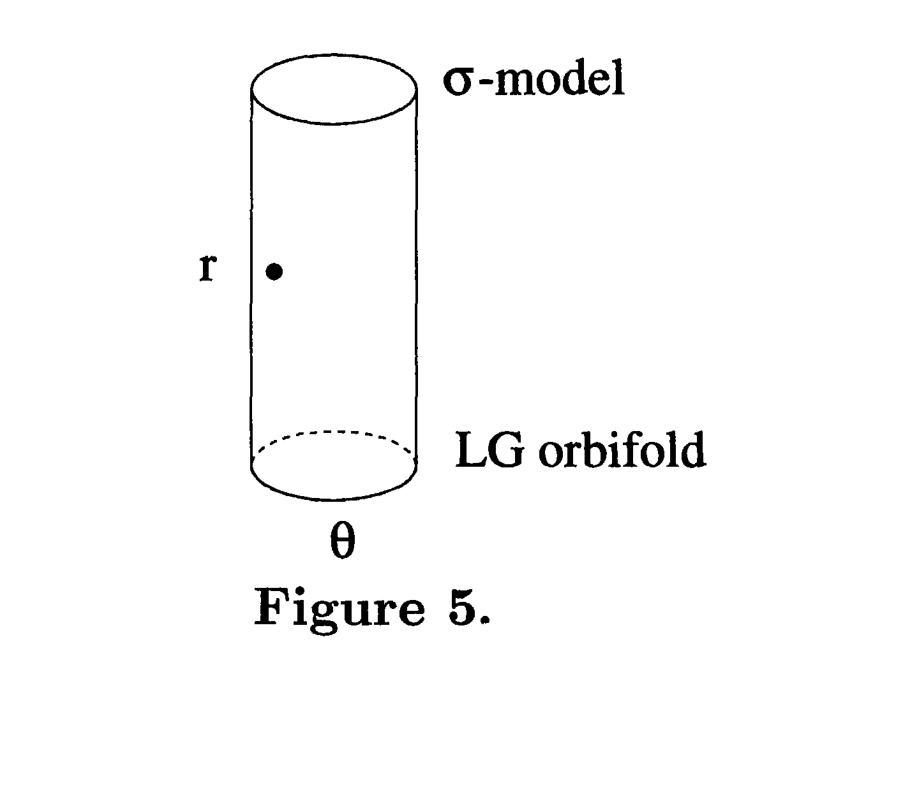
\includegraphics[width=0.40\textwidth]{figs/fig_p215_1.png}
  \caption{$r$--$\theta$ 柱面：竖直方向为 $r$，绕柱的圆周方向为 $\theta$。柱顶标注 $\sigma$-model（$r\gg0$ 的一端），柱底标注 LG orbifold（$r\ll0$ 的一端）；柱面上的黑点示意量子理论出现奇异的位置，对应 $r=r_0$、$\theta=0$。（原文 Figure 5，p.215）}
  \label{fig:p215-1}
\end{figure}

% 原文 pp.216–222（印刷 pp.1334–1340）
% 承接第 15 讲第 1 部分：本文件自 §15.2 末段（p.216）起，经 §15.3–§15.8，至 p.222 的「参考文献与交叉引用」止；
% 因属同一讲的后续分段，故不写 \section，直接从正文与 \subsection 开始。
% 本 7 页内没有任何 Figure / 示意图，故无插图。

% ===== 原文 p.216 =====
% （本页首句承接 p.215 末段：关于此类 Calabi--Yau 流形的椭圆亏格与 Landau--Ginzburg 侧极小模型特征标的比较。）

椭圆亏格（elliptic genus）应当与 $t$ 无关，因为它是拓扑不变量；由此可以得到一个公式，把这一类 Calabi--Yau 流形的椭圆亏格，与 Landau--Ginzburg 一侧可由极小模型（minimal model）的特征标（character）显式算出的椭圆亏格联系起来。

尽管椭圆亏格与 $t$ 无关，我们讨论过的 $\mathcal{N}=2$ 理论中的另一个量——$Q_t$-上同调（$Q_t$-cohomology）——却随 $t$ 全纯地变化。这个问题中的瞬子（instanton），也就是 $\sigma$ 模型中的全纯曲线（holomorphic curve），会给路径积分贡献一个因子
\[
  \exp\Bigl(-i\theta\int\frac{F}{2\pi}-r\int d^2x\,D\Bigr),
\]
其中 $D=\sum_j\alpha_j|\Phi_j|^2-r$。$\mathcal{N}=2$ 模型的瞬子方程——即场在某个超对称下保持不变的条件——给出 $\int d^2x\,D=\int F/2\pi$，于是这个因子就是 $\exp\bigl(-2\pi it\int_\Sigma\Phi^*(c_1(\mathcal{L}))\bigr)$。我们将在本讲的后半部分探讨这些瞬子求和。

% [Tutor Note: 这里两处 $r$ 项相差一个 $2\pi$，是极易踩空之处。由 $\int d^2x\,D=\int F/2\pi=\int_\Sigma\Phi^*(c_1(\mathcal{L}))=n$，本页显示公式给出 $\exp(-irn-i\theta n)$；而 p.220 把复参数取为 $t=-ir+\theta/2\pi$，于是 $\exp(-2\pi itn)=\exp(-2\pi irn-i\theta n)$，二者在 $r$ 项上差因子 $2\pi$。要使两式一致，需把 FI 参数以 $1/2\pi$ 为单位（即 $t=\theta/2\pi-ir/2\pi$），或等价地认为 $D$ 项积分自带 $1/2\pi$ 归一化。核对第 13 讲线性 $\sigma$ 模型公式时务必先固定这一归一化，否则 p.221 的幂等元位置 $\sigma=\mu e^{2\pi i(-t+k)/n}$ 会整体错位；这与 p.221 脚注 5 所讨论的「物理归一化 vs.\ 拓扑归一化」属同一类问题。]

\subsection{量子上同调的引入}
% 原文 §15.3：Introduction to quantum cohomology

现在回到二维的扭曲（twisted）$\mathcal{N}=2$ 超对称 $\sigma$ 模型，其靶空间（target）是 Kähler 流形 $X$。回忆一下：依所保留的超对称荷 $Q\in\{\overline{Q}_+ + Q_-,Q_+ + Q_-,Q_+ + \overline{Q}_-,\overline{Q}_+ + \overline{Q}_-\}$ 的不同，共有四种扭曲方式。

% [Tutor Note: 扫描件（p.1334）中集合里几个 $Q$ 的上划线极细、几乎无法分辨，字面上会出现同一元素重复三次的无意义结果。按上下文——四种扭曲对应 $(a,a),(c,a),(a,c),(c,c)$ 四个手征环，且 p.217 明确说「今天只考虑使 $\overline{Q}_+ + Q_-$ 成为整体的扭曲」（情形 A，即 $(a,a)$ 环）——这四项应是 $\overline{Q}_\pm$ 与 $Q_\pm$ 的两两配对，译文按此恢复。若以扫描件字面为准逐字转写，须自行把缺失的上划线补回，否则后面谈「$(a,a)$ 环由 $Q=\overline{Q}_+ + Q_-$ 定义」时会自相矛盾。]

无论选择哪一种，$Q$ 的上同调作为向量空间都可与 $X$ 的上同调等同。但其中还有更多结构：若把 Riemann 面固定为某个二维流形 $\Sigma$，则额外的结构是 $Q$ 的上同调上的一个环结构。所得的环分别称为 $(a,a)$、$(c,a)$、$(a,c)$ 与 $(c,c)$ 手征环（chiral ring）。

在其中一个选择下，手征环的经典版本恰好就是上同调上通常的环结构；但在量子力学层面，对这个经典答案还有修正，即瞬子修正。正因如此，$\sigma$ 模型的手征环被称为 Kähler 流形 $X$ 的量子上同调（quantum cohomology）。在本讲的后半部分，我们将一般地讨论量子上同调，然后在 $X=\mathbb{CP}^{n-1}$ 以及 $X$ 为 Fano 超曲面的情形做一些显式计算。这些计算既从数学上做——即数具有某些性质的全纯有理曲线；也从物理的观点做：利用重整化群流（在第 13 讲与本讲前半部分讨论过），把这些 $\sigma$ 模型流向带有额外真空的 Landau--Ginzburg 理论。

\subsection{零能态的空间}
% 原文 §15.4：The space of zero-energy states

我们想计算其中一些手征环。但在直接处理算符之前，我们先在 Hamilton 框架下计算零能态（zero-energy states）。之所以要做这个计算，是因为如第 14 讲 §14.3.3 所示，存在一个映射
\[
  \psi:\ \text{手征环}\longrightarrow\{\text{零能态}\},
\]
它由在半球面上某点插入一个局域算符给出。在有利的情形下，这个映射是同构。

% ===== 原文 p.217 =====

在 Hamilton 框架下，场空间底下的玻色子空间是
\[
  \mathcal{W}=\operatorname{Maps}(S^1,X).
\]
能量最低的位形是常值映射；这些位形的空间就是 $X$ 的一份拷贝。由于旋量丛（spin bundle）的两份拷贝中各有费米子，量子化之后所得的 Hilbert 空间是 $X$ 上旋量丛两份拷贝的张量积，亦即 $X$ 上的微分形式空间。Hamiltonian 就是 Laplacian，于是它的基态空间是 $X$ 上的 $L^2$ 调和形式空间，后者与 $H^*_{L^2}(X)$ 等同。当然，还要考虑 $\mathcal{W}$ 中这份 $X$ 的法方向；但超对称意味着法方向上的二次型非退化，于是这些方向给出谐振子的张量积，并具有唯一的基态。因此在最后我们发现：整个理论的基态与 $X$ 上的调和形式等同。我们将看到，手征环的计算（在加法的意义上）给出同样的答案，于是在今天所考虑的情形里，映射 $\psi$ 确实是同构。一般地，只要经典理论具有「能量随场趋于无穷而增长」这一性质，上述结论就成立。\footnote{对于靶空间 $X$ 紧致的 $\sigma$ 模型，一个映射 $\Phi:S^1\to X$「趋于无穷」的唯一含义只是它可以沿 $S^1$ 变化得极为剧烈；这当然会使能量增长。（原文 p.217 页脚注）}

% [Tutor Note: 脚注原文作 ``the only sense in which a map $\Phi:S^1\to X$ can `go to infinity' is that \emph{they} can become rapidly varying along $S^1$''，主语 a map 与代词 they 不一致，应为 it，属排印疏漏。物理上要紧的是后半句：靶空间紧致时不存在「场趋于无穷」的通常含义，唯一可能是 $\Phi$ 沿 $S^1$ 剧烈振荡，此时能量 $\int_{S^1}|d\Phi|^2$ 确实发散。这正是保证 $\psi$ 为同构、并使超对称量子力学中 Witten 指标论证成立的关键（参见 E. Witten, J.\ Diff.\ Geom.\ 17 (1982) 661 关于超对称量子力学与 Morse 理论的工作）；若靶空间非紧，这一论证失效，$\psi$ 一般只是单射。]

\subsection{手征环的一般性质}
% 原文 §15.5：Generalities on the chiral ring

为定义手征环，我们需要一个平方为零的整体超对称。如第 14 讲 §14.3 所见，选取 $\mathcal{N}=2$ 超对称理论的某种扭曲形式，就会选出这样一个整体超对称。今天我们将只考虑使 $\overline{Q}_+ + Q_-$ 成为整体超对称的扭曲；这就是第 14 讲中所说的「情形 A」（Case A）。这种扭曲对任何 Kähler 流形都可施行——无需假定第一 Chern 类为零。我们将考虑这样的局域算符：它们是基本玻色场 $\Phi:\Sigma\to X$（$\Sigma$ 是我们的 Riemann 面）以及由超对称与 $\Phi$ 相联系的费米子的函数。（若在 $X$ 上取局部坐标，则我们用 $S^1$ 上的一族函数 $\phi_j$ 来描述 $\Phi$。）回忆扭曲的效应之一，是使费米子成为整自旋而非半自旋丛的截面；也就是说，它们不再是旋量，而是 $\Sigma$ 上的微分形式（取值于 $X$ 切丛的拉回）。在描述算符的 $Q$-上同调时，只需考虑零自旋的费米子。理由在于：所有 $Q$-上同调类的算符都有仅用这些费米子构造的代表元。更确切地说，$Q$-上同调类具有只依赖玻色场与零自旋费米子、而不依赖其导数的代表元。\footnote{这是如下事实的算符版本：在 Hamiltonian 描述中，零能态由靶空间上的微分形式构造，其中所有振子都处于基态；含场导数的算符则对应于某些振子被激发的态。（原文 p.217 页脚注）} 于是，我们的局域算符将具有形式
\[
  \mathcal{O}=\mathcal{O}(\phi,\psi_L,\psi_R),
\]
其中，在未扭曲的版本中，$\psi_L$ 是 $K^{-1/2}\otimes\phi^*T^{0,1}X$ 的截面，而 $\psi_R$ 是 $K^{1/2}\otimes T^{1,0}X$ 的截面。扭曲之后，这些费米子场位于 $\Phi^*T^{0,1}X$ 与 $\Phi^*T^{1,0}X$ 中，因为扭曲把 $\Sigma$ 上的线丛抵消掉了。特别地，

% [Tutor Note: 此处原文的 $\psi_R$ 写作 $K^{1/2}\otimes T^{1,0}X$，漏掉了拉回 $\phi^*$；紧接的「扭曲后位于 $\Phi^*T^{0,1}X$ 与 $\Phi^*T^{1,0}X$」一句可证应为 $K^{1/2}\otimes\phi^*T^{1,0}X$。另注意 $\psi_L$ 与 $\psi_R$ 携带的 $K$ 幂次相反（$-1/2$ 与 $+1/2$），这并非笔误：正因二者相反，同一个扭曲才能把它们同时抵消成 $\Phi^*T^{0,1}X$、$\Phi^*T^{1,0}X$ 的截面；若写成相同的幂次，扭曲后必残留一个 $\Sigma$ 上的线丛，$Q$ 就不再是 $\Sigma$ 上的标量超荷，$Q$-上同调也不再等于 $X$ 的 de Rham 上同调。再者，括号里说「用 $S^1$ 上的函数描述 $\Phi$」疑为 $\Sigma$ 之误：$\Phi$ 是 $\Sigma\to X$ 的映射，p.218 的 $\mathcal{O}_\lambda(x)=f_\lambda(\phi(x),\psi(x))$ 中 $x$ 属于 $\Sigma$；$S^1$ 的说法只适用于本页的 Hamiltonian 图像。]

% ===== 原文 p.218 =====

就可以组成和 $\psi=\psi_L+\psi_R$，并考虑算符 $\mathcal{O}=\mathcal{O}(\phi,\psi)$，其中 $\psi$ 是 $\Sigma$ 上的零形式，取值于 $TX=T^{1,0}X\oplus T^{0,1}X$ 的拉回。

\subsubsection{局域算符}
% 原文 §15.5.1：Local Operators

$X$ 上的每个微分形式 $\lambda$ 都对应一个函数 $f_\lambda(\phi,\psi)$（$f_\lambda$ 是 $\Pi TX$ 上的函数）。于是对每个 $\lambda$ 都有一个算符 $\mathcal{O}_\lambda(x)=f_\lambda(\phi(x),\psi(x))$。正如上周那一讲所提到的，在算符与形式的等同之下，$Q$ 等同于通常的外微分：
\[
  \{Q,\mathcal{O}_\lambda\}=\mathcal{O}_{d\lambda}.
\]
这就是为什么在加法的意义上，$Q$-上同调与 $X$ 的 de Rham 上同调一致。

% [Tutor Note: 这里的等同 $Q\leftrightarrow d$ 是整套「物理 $\leftrightarrow$ 数学」词典的核心，符号上易错者有两点。(i) $Q$ 与 $\mathcal{O}_\lambda$ 都是费米型算符（$\lambda$ 为奇次时 $\mathcal{O}_\lambda$ 亦然），故用反对易子 $\{Q,\mathcal{O}_\lambda\}=\mathcal{O}_{d\lambda}$；若误写成对易子，或忽略了 $d\lambda$ 前的符号随 $\deg\lambda$ 的变化，整体会差一个 $(-1)^{|\lambda|}$。(ii) $f_\lambda$ 是 $\Pi TX$（切丛的奇（parity）版本，纤维坐标 $\psi$ 反对易）上的函数，即「$\psi$ 的多项式 $=$ 微分形式」；而 $\lambda$ 的 de Rham 类与 Poincaré 对偶闭链 $H_i$ 的配对约定，直接决定 p.218–219 瞬子计数中 $\pm1$ 的符号（等价于 determinant line bundle 的定向选取），不同文献的符号可能整体相反。]

当算符—态对应是同构时——正如在这些 $\mathcal{N}=2$ 超对称 $\sigma$ 模型的情形——我们可以通过计算关联函数来计算手征环的环结构。这里的目标是用更经典的拓扑与几何语言来计算关联函数
\[
  \langle \mathcal{O}_{\lambda_1}(x_1)\cdots\mathcal{O}_{\lambda_s}(x_s)\rangle,
\]
其中 $\lambda_i$ 是闭形式。我们已经指出，若把 $\lambda_i$ 换成上同调等价的形式，关联函数不变。此外，要计算这个关联函数，也就是计算路径积分
\[
  \int \mathcal{D}\phi\,\mathcal{D}\psi\,e^{-\mathcal{L}}\prod_i\mathcal{O}_{\lambda_i}(x_i)
\]
（积分遍历所有场），只需把它化为在 $Q$-不变场子空间上的积分即可。我们已经辨认出 $Q$-不动点子空间的玻色部分：它就是全纯映射 $\Sigma\to X$ 的空间。对每个 $i$ 取一个与 $[\lambda_i]$ Poincaré 对偶的闭链 $H_i$；于是可以选取 $\lambda_i$ 的一个代表元，使其支集落在 $H_i$ 的任意小邻域内。

现在我们要通过把路径积分定域化（localization）到 $Q$-不变的经典位形上、即定域化到 Riemann 面到 $X$ 的全纯映射上，来计算关联函数。给定我们所选的算符代表元，只有那些在点 $x_i$ 处穿过 $H_i$ 的全纯映射才有贡献。在「最好」的情形，即过这些点的全纯映射的模空间由有限个非退化点组成时，可以证明每个这样的映射贡献 $\pm1$。事实上，超对称保证 Bose 行列式与 Fermi 行列式相消，只剩一个符号。于是，对所有全纯映射求和所得的结果，等于经典作用量的指数因子与来自行列式的符号之积。对全纯映射而言，经典作用量的指数因子恰好是 $\exp\bigl(-2\pi it\int_\Sigma\Phi^*(c_1(\mathcal{L}))\bigr)$。

% [Tutor Note: 「每个非退化映射贡献 $\pm1$」是高度压缩的结论，其依据是 Atiyah--Bott 定域化（等价地，超对称量子力学中的 Witten 不动点/指标公式）：路径积分在 $Q$-不变位形附近展开时，Bose 与 Fermi 的非零模成对出现、行列式之比为 $\pm1$，只剩符号。要定出符号，须为每个分支的 determinant line bundle 指定定向——本段「up to sign」正是回避了这一约定。还需注意：若模空间含非平凡自同构（例如恰有额外对称的映射），「有限个非退化点」的前提不成立，此时必须改用等变（equivariant）版本或虚拟基本类计数，这正是后来 Gromov--Witten 不变量的出发点（参见 Kontsevich 关于稳定映射与虚模空间的工作）。]

从数学上说，要使「在 $x_i$ 处穿过 $H_i$ 的全纯映射」这一问题给出零维模空间，必须满足一个维数计数。更一般地陈述：若把算符 $\mathcal{O}_{\lambda_i}(x_i)$ 解释为在 $\Sigma\to X$ 的所有全纯映射的模空间上产生微分形式，则 $H_i$ 须满足一个维数条件，该微分形式才是最高次形式；否则其积分必然为零。从物理观点看，同样的维数限制来自 $R$ 对称性的反常：路径积分中的积分测度在该对称性下有反常，因此必须选用这样一组算符，使其乘积

% ===== 原文 p.219 =====

恰具有可以抵消的反常，路径积分才有非零的可能。毫不奇怪，这两个条件是同一个条件：即 $X$ 中诸 $H_i$ 的余维（codimension）之和，必须等于我们所考虑的那个全纯映射模空间分支的虚拟维数（virtual dimension）。

若只想看到经典的上同调环而非量子上同调，则应取 $\Sigma$ 亏格为零，并且只考虑映入 $X$ 的常值映射。当然，常值映射恰好填满 $\operatorname{Maps}(\Sigma,X)$ 的某一分支中的全部全纯映射，即由零伦（null-homotopic）映射构成的那个分支。对这个同伦类中的映射，维数条件是
\[
  \sum_{i=1}^{s}\deg\lambda_i=\dim X,
\]
而经典答案就是
\[
  \int_X\lambda_1\wedge\cdots\wedge\lambda_s.
\]
也就是说，经典手征环就是 $X$ 的上同调环。这个答案在量子力学上会被瞬子修正所修正，修正量由我们刚才描述的那些在非常值全纯映射模空间上的积分给出。因此，手征环是对 $X$ 通常上同调环的量子修正；正因如此，手征环通常被称为 $X$ 的量子上同调环。

% [Tutor Note: 「常值映射恰好填满某一分支中的全部全纯映射」一句容易读成「常值映射构成全体全纯映射」，关键限定语是「某一分支」：$\operatorname{Maps}(\Sigma,X)$ 按同伦类分成分支，常值映射恰好填满零伦分支中的全部全纯映射。理由是全纯映射的能量 $\int_\Sigma|d\Phi|^2$ 只依赖 $\Phi_*[\Sigma]$ 所代表的同调类，在零伦类上必须为零，于是 $d\Phi\equiv0$。再与 p.220 的维数条件对照：那里 $a+b+c=n-1+dn$ 而 $\deg\sigma=2$，真正饱和虚拟维数的是 $\sum_i\deg\lambda_i=2(a+b+c)$，即带三个标记点的映射模空间的虚拟维数 $2(n-1+dn)$；文中「$=\dim\mathcal{M}_d$」若按不带标记点的模空间理解则为 $nd+n-4$，相差的 $3$ 正来自三个标记点（$\mathrm{Aut}(\mathbb{P}^1)$ 的三维）。这几个 $2$ 与 $3$ 是抄录维数条件时最常见的错误来源。]

\subsection{环结构的更多细节}
% 原文 §15.6：More Details on the Ring Structure

在给出量子上同调作为手征环的一般定义、并说明了计算它所需的数学之后，现在该更具体一些、算一个例子了。我们取 $\Sigma=S^2$ 映入紧 Kähler 流形 $X$ 的情形。先从一个只有两个算符的关联函数开始：
\[
  \langle \mathcal{O}_{\lambda_1}\mathcal{O}_{\lambda_2}\rangle,
\]
其中 $\lambda_1$ 的次数加上 $\lambda_2$ 的次数等于 $X$ 的维数。我们当然知道，常值映射的空间对这个关联函数的贡献等于
\[
  \int_X\lambda_1\wedge\lambda_2.
\]
在这种情形没有量子修正，这也就是手征环中的答案。没有量子修正的理由是：映入 $X$ 的非常值全纯映射 $S^2\to X$（并指定点 $x_1,x_2\in S^2$ 分别映到 $H_1$ 与 $H_2$）构成的空间上有一个自由的 $\mathbb{C}^*$ 作用，它由 $S^2$ 上固定 $x_1,x_2$ 的 $\mathbb{C}^*$ 作用诱导而来。该空间的某个分支要对关联函数给出非零修正，其形式维数（formal dimension）必须为零。若其实际维数为零、其上又有自由 $\mathbb{C}^*$ 作用，则它必为空集。（即便该空间可能有非空的分支，自由 $\mathbb{C}^*$ 作用也保证其贡献为零。）于是，在手征环与 $X$ 上同调的等同之下，两点关联函数——它计算手征环底下向量空间上的内积——给出上同调上通常的内积，等价地给出同调上的相交形式（intersection form）。

% ===== 原文 p.220 =====

现在来考虑环结构。取 $H^*(X)$ 的一组基 $\{\lambda_i\}$，设在这组基下内积由 $\eta_{ij}$ 给出：
\[
  \eta_{ij}=\langle \mathcal{O}_{\lambda_i}\mathcal{O}_{\lambda_j}\rangle.
\]
于是环结构由结构常数（structure constants）$c_{ij}^k$ 决定：
\[
  \mathcal{O}_{\lambda_i}\mathcal{O}_{\lambda_j}=c_{ij}^k\,\mathcal{O}_{\lambda_k}.
\]
令 $\omega_{ijk}$ 为三点函数
\[
  \omega_{ijk}=\langle \mathcal{O}_{\lambda_i}\mathcal{O}_{\lambda_j}\mathcal{O}_{\lambda_k}\rangle.
\]
由于这个三点函数也是前两个局域算符之积与第三个的内积，我们看到
\[
  \omega_{ijk}=\sum_{r}c_{ij}^r\,\eta_{rk}.
\]
由于 $\eta_{ij}$ 非退化，这说明两点与三点关联函数决定了手征环的环结构。

\subsection{$\mathbb{CP}^{n-1}$ 的计算}
% 原文 §15.7：Calculations for $\mathbf{CP}^{n-1}$

现在来看一个例子。我们借助规范线性 $\sigma$ 模型（gauged linear sigma model）来计算 $\mathbb{CP}^{n-1}$：规范群为 $U(1)$，线性玻色场为 $\phi_1,\dots,\phi_n$，如第 13 讲 §13.4 那样（那一讲中这些场记作 $A_i$）。要得到整个 $\mathbb{CP}^{n-1}$，我们令超势 $W$ 等于零。这样得到一族依赖于复参数 $t=-ir+\frac{\theta}{2\pi}$ 的理论；如我们所见，当 $\operatorname{Im}(t)\ll0$ 时，它们是 $X$ 上的非线性 $\sigma$ 模型，其 Kähler 度量依赖于 $t$，而 Kähler 类大致正比于 $\operatorname{Im}(t)$。唯一的可观测量是 $\mathcal{O}_H$，其中 $H$ 是超平面截影（hyperplane section）。我们把这个算符记作 $\sigma$。经典地，在 $\mathbb{CP}^{n-1}$ 中我们有一个关系，即 $\sigma^n=0$。让我们看看量子力学上会发生什么。我们需要计算三点函数
\[
  \langle\sigma^a\sigma^b\sigma^c\rangle,
\]
其中 $a+b+c=n-1+dn=\dim\mathcal{M}_d$，即 $d$ 次有理曲线模空间的维数。显然，只需考虑 $a,b,c<n$ 的情形。这意味着 $d$ 只可能取 $d=0,1$。当然，$d=0$ 是常值映射的模空间，其贡献就是经典的环结构。对 $d=1$，我们考虑的是 $\mathbb{CP}^{n-1}$ 中的直线。为计算
\[
  \langle\sigma^{n-1}(x)\sigma^{n-1}(y)\sigma(z)\rangle,
\]
我们必须考虑过两点的直线中与某个固定超平面相交的那些；这样的直线恰好有一条。由于瞬子作用量为 $e^{-2\pi it}$，这给出关系
\[
  \langle\sigma^{n-1}(x)\sigma^{n-1}(y)\sigma(z)\rangle=e^{-2\pi it}.
\]
从这个三点函数反解出环结构，得到量子上同调中的
\[
  \sigma^n=e^{-2\pi it}.
\]
我们也可以用物理方式做同样的计算。我们考虑的是 $\sigma$ 模型 $\mathbb{CP}^1\to\mathbb{CP}^{n-1}$。在第 13 讲 §13.6.2 中我们发现，它在红外流向 $n$ 个有能隙的真空（因为这是 $c_1(X)>0$ 的情形，

% [Tutor Note: 注意 $d=0$ 与 $d=1$ 两项的分工：$d=0$ 给经典关系 $\sigma^n=0$，$d=1$ 给关系 $\sigma^n=e^{-2\pi it}$。而「$a,b,c<n$ 已经足够」的理由是：任取 $a\ge n$，都可用 $\sigma^n=q$ 反复约化到更低次，故三点函数只依赖 $\sigma$ 的幂次模去关系——这正是「从三点函数反解环结构」的实际操作。易错点有二：(i)「过两点的直线与固定超平面相交者恰有一条」在 $n\ge3$ 时成立，但 $n=2$（即 $\mathbb{CP}^1$）时「超平面」退化为点，几何退化，故 $n=2$ 时 $\sigma^n=e^{-2\pi it}$ 的 $d=1$ 部分须另行核验；(ii) 指数上是 $e^{-2\pi it}$，符号来自 $t=-ir+\theta/2\pi$ 与 $\theta$ 项 $-i\theta\int F/2\pi$ 的约定；若某文献取 $t=\theta/2\pi+ir$，同一关系会被写成 $q=e^{2\pi it}$，对读时极易差一个整体符号。]

% ===== 原文 p.221 =====

流是从 $\sigma$ 模型流向 Landau--Ginzburg 模型）。场 $\sigma$ 在每个真空中取不同的期望值。由于诸场有质量，我们干脆把它们取为各自的期望值。这些真空期望值为 $\sigma=\mu e^{2\pi i(-t+k)/n}$，$k=0,\dots,n-1$。它们给出量子上同调环的幂等元（idempotents），由此我们推得与前面相同的答案，\footnote{除 $\mu$ 的一个幂次之外——这源于我们的物理约定与数学约定之间的不匹配。在第 13 讲中，$\sigma$ 被定义为一个量纲为一的场，且并未试图把它与任何拓扑归一化相比较。而在今天的数学讨论中，$\sigma$ 是按拓扑方式归一化的，即作为与射影空间的超平面截影相联系的场，因此其量纲为零。要比较这两个定义，应在第 13 讲的框架下，在 $r\gg0$ 的区域把 $\sigma$ 场积掉，以换得 $\sigma$ 模型的无质量场。在此过程中，$\sigma$ 将变成低能理论的一个算符，该算符可由 $\mathbb{CP}^{n-1}$ 上的一个 2-形式导出。这个算符的上同调类将是超平面截影的某一倍数 $C$，而 $C$ 正是第 13 讲的物理归一化与「给出 $\sigma^n=e^{-2\pi it}$ 的拓扑归一化」不相符的因子。（原文 p.221 页脚注）} 即该环由 $\sigma$ 生成，并服从关系 $\sigma^n=e^{-2\pi it}$。

\subsection{Fano 超曲面的计算}
% 原文 §15.8：Calculations for Fano Hypersurfaces

现在把这些计算推广到 $\mathbb{CP}^{n-1}$ 中次数 $d<n$ 的超曲面，即所谓的 Fano 超曲面。

据 [A. Collino and M. Jinzenji, \emph{On the structure of small quantum cohomology rings for projective hypersurfaces}, preprint hep-th/9611053.]，用数学方法算出的答案是：超平面截影 $\sigma$ 服从如下关系：
\begin{equation}
  \tag{15.1}
  \label{eq:15-1}
  \sigma^{d-1}\bigl(\sigma^{n-d}-e^{-2\pi it}\bigr)=0.
\end{equation}

让我们想一想，这个计算如何与下述事实相容：这个 $\sigma$ 模型在红外同样流向一个 Landau--Ginzburg 模型，再加上额外的一些有质量真空。方程 $\sigma^{d-1}\bigl(\sigma^{n-d}-e^{-2\pi it}\bigr)=0$ 的根有两类：$\sigma=0$ 处一个重数为 $d-1$ 的根，以及 $\sigma\ne0$ 处的非退化根（即重数为一的根）。方程的根对应于量子场论的真空。非退化根对应于有质量真空，它们给出量子上同调环的幂等元。在第 13 讲 §13.6.2 中分析该理论的真空结构时，我们找到 $\sigma\ne0$ 处的 $n-d$ 个有质量真空。它们位于 $e^{-2\pi it}$ 的 $(n-d)$ 次根处（再乘以一个常数，其解释与上一条脚注相同），并给出量子上同调方程中的因子 $\bigl(\sigma^{n-d}-e^{-2\pi it}\bigr)$。另一个因子 $\sigma^{d-1}$ 是原点处 Landau--Ginzburg 真空的贡献。这个因子在 $d>1$ 时出现（对 $d=1$，我们讨论的是余维为一的射影空间，没有 Landau--Ginzburg 真空）；当 $d>2$ 时，它对应于原点处一个重数大于一的根。这一限制的理由从物理上看很清楚：对 $d=2$，Landau--Ginzburg 理论的中心荷（一般情形为 $\hat c=n(1-2/d)$）为零，因此这时 Landau--Ginzburg 理论有质量、在红外是平庸的。对 $d>2$，Landau--Ginzburg 理论有一个非平凡临界点，它自然可以贡献一个重数大于一的根。由于标度不变性，这个根将位于原点。如何计算 Landau--Ginzburg 轨形（orbifold）的上同调，在其中一个习题中有描述；有了那些结果，就可以算出眼前这个情形中根的重数。

% [Tutor Note: 检验 (15.1) 是否漏项的最快办法是数根（计重数）：$(n-d)+(d-1)=n-1$，恰等于 $X$ 的上同调总维数——$X$ 是 $\mathbb{CP}^{n-1}$ 中次数 $d$ 的超曲面，复维 $n-2$，故 $H^*(X)$ 由 $1,H,\dots,H^{n-2}$ 张成，共 $n-1$ 个类，与量子化后真空（幂等元）数应当一致。若把 $\sigma^{d-1}$ 误抄成 $\sigma^{d-2}$，或把 $e^{-2\pi it}$ 的根数 $(n-d)$ 与 $n$ 搞混，这个计数立刻对不上。另可注意：原文说「$d>2$ 时该根重数大于一」，而 $d=2$ 时 $\hat c=0$、LG 理论有质量，故 $\sigma^{d-1}=\sigma$ 的根重数为一，两者自洽。]

% ===== 原文 p.222 =====

\subsection*{参考文献与交叉引用}
% 原文：References and cross references

本讲大部分内容的一个参考文献是

E. Witten, \emph{On the Landau--Ginzburg description of $\mathcal{N}=2$ minimal models}, Int.\ J.\ Mod.\ Phys.\ A \textbf{9} (1994), pp.\ 4783--4800.

关于 Landau--Ginzburg 及相关模型的椭圆亏格的进一步计算，参见

P. Berglund and M. Henningson, \emph{On the Elliptic Genus and Mirror Symmetry}, in \emph{Essays on
Mirror Manifolds II}, ed.\ S.-T. Yau (International Press), and references therein.


\clearpage
% 原文 pp.223–232（印刷 pp.1341–1350）
\section{Lecture 16：四维规范理论}

\begin{keytakeaways}
本讲以欧氏号差的四维规范场论为对象，先从无超对称的纯 Yang--Mills 理论与带 $n_f$ 味的 $SU(N)$ 理论入手，说明红外行为（质量间隙、禁闭）目前仍只能「相信」与「猜测」；核心数学工具是味对称性 $U(n_f)\times U(n_f)$ 的反常破缺、Goldstone 定理，以及流的三点函数所携带的不变三次型 $d^{abc}$——后者给出一个纯粹由短距离计算得到的无质量判据。随后转入 $\mathcal{N}=1$ 超对称纯规范理论，借助超空间表述、全纯性与瞬子，论证手征对称性 $\mathbb{Z}/2h\mathbb{Z}$ 自发破缺出 $h$ 个真空，并由 $\langle\operatorname{Tr}\lambda\lambda\rangle$ 的标度行为反推出 $\beta$ 函数的一圈精确性。最后在 $\mathcal{N}=1$ SQCD 中按 $k=n_f$ 分区讨论红外相，用「下降」程序、量纲与全纯性定出超势 $W=c_{n,k}(\det M)^{-1/(n-k)}$，并指出 $c_{n,n-1}\ne0$ 来自单瞬子计算。全讲的主线是：反常与瞬子这类「短距离/拓扑」信息，足以严格约束甚至决定红外物理。
\end{keytakeaways}

% ===== 原文 p.223 =====

本讲我们将纵览四维规范场论中一些主要的、已知的、被相信的与被猜测的结果，无论是否带有超对称。

\subsection{无超对称的规范理论}
% 原文 §16.1：Gauge theory without supersymmetry

我们从没有超对称（$\mathcal{N}=0$）的情形开始。先考虑单 Lie 群 $G$ 的纯非阿贝尔规范场论（pure nonabelian gauge theory），其拉格朗日量为
\[
L=\frac{1}{4g^2}\int\operatorname{Tr}F\wedge *F .
\]
我们还可以加上带 $\theta$ 角（theta angle）的拓扑项 $\frac{i\vartheta}{16\pi^2}\int\operatorname{Tr}F\wedge F$。这是一个定义良好、渐近自由（asymptotically free）的理论。我们所关心的问题是：这个理论在红外（infrared）端如何行为。

人们相信（对一切 $\vartheta$）这个理论具有质量间隙（mass gap），并猜测它表现出禁闭（confinement）（Wilson 圈算符的面积律，见第 6 讲）。然而，要证明第一个断言、尤其是第二个断言，至今仍是一个重要的未解决问题。

\textbf{Remark.} 正如我们将看到的，超对称的好处在于：在超对称规范场论中，这两个断言至少可以部分地得到证明。

现在让我们加入物质（matter）。本讲采用欧氏号差（Euclidean signature）。先看群为 $G=SU(N)$ 的例子。取物质场为取值于矢量表示 $V$ 与对偶表示 $V^*$ 的手征旋量（chiral spinor）$\psi_i,\psi_i^*$，以及取值于 $V^*$ 与 $V$ 的相应反手征旋量（antichiral spinor）$\bar\psi_i,\bar\psi_i^*$。（手征旋量与反手征旋量分别是取值于给定表示的正、负旋量丛 $S_+$ 或 $S_-$ 的截面。）设每种旋量的个数为 $n_f,n_f^*$（即味（flavor）的数目）。为避免局域反常（local anomaly），必须有 $n_f=n_f^*$（见下一讲）。

带旋量的理论（裸质量为零）的拉格朗日量为
\begin{equation}
  \tag{16.1}
  \label{eq:16-1}
  L=\frac{1}{4g^2}\int\operatorname{Tr}F\wedge *F+\frac{i\vartheta}{16\pi^2}\int\operatorname{Tr}F\wedge F+\sum_i\int\Bigl[(\bar\psi_i,D\psi_i)+(\bar\psi_i^*,D\psi_i^*)\Bigr].
\end{equation}

% [Tutor Note: 记号 $\psi_i^*$ 极易误读。它是与 $\psi_i$ 相互独立的第二个手征旋量（取值于对偶表示 $V^*$），并不是 $\psi_i$ 的厄米共轭；$\psi_i$ 的反手征伙伴是 $\bar\psi_i$。正因如此，$V$ 与 $V^*$ 中的手征旋量味数必须相等（$n_f=n_f^*$），局域反常才能抵消——原文此处说"见下一讲"，即第 17 讲对局域反常的系统讨论。另：本页原文 "The take the matter fields to consist of..." 中 "The take" 显然是 "We take" 的笔误，译文按后者处理。]

% ===== 原文 p.224 =====

\textbf{Remark.} 当 $G=SU(3)$ 且 $n_f=2$ 或 $3$ 时，这就是强相互作用的理论。在这些情形下，若要精确地描述强相互作用，我们其实应当加入小的费米子裸质量。

若 $n_f$ 不太大，该理论是渐近自由的。因此人们关心它的红外行为。

该拉格朗日量具有作用在味上的整体 $U(n_f)\times U(n_f)$ 对称性。然而在量子层面，这个理论有手征反常（chiral anomaly）（因为手征旋量上的 Dirac 算符可以有非零指标（index））。因此，量子力学上算符代数的对称性被破缺到子群 $H=\{(A,B)\in U(n_f)\times U(n_f):\det(A)=\det(B)\}$（群的其余部分被破缺，是因为在瞬子（instanton）场中，它不能使路径积分的测度保持不变）。

人们相信，当 $n_f>1$ 时，群 $H$ 自发破缺（spontaneous symmetry breaking）到 $U(n_f)\times U(n_f)$ 的对角子群 $H_{\mathrm{diag}}$，并由 Goldstone 定理导致 Goldstone 玻色子（Goldstone boson）的存在。注意对角子群正是允许费米子有裸质量的最大子群。若 $n_f\le1$，$H$ 本身已经是对角的，我们就得不到任何自发对称性破缺或 Goldstone 玻色子。在这种情形下，人们相信理论有质量间隙。对 $n_f>1$，Goldstone 玻色子的存在意味着不可能有质量间隙。此时人们相信理论是红外自由的（infrared free），并且除 Goldstone 玻色子之外没有别的无质量粒子；于是低能有效理论是真空空间 $H/H_{\mathrm{diag}}$ 上的一个 $\sigma$ 模型。若再为费米子加上小的裸质量、以使模型更好地描述自然，那么（正如某道习题所探讨的）一般会挑出一个唯一的真空，并由此产生质量间隙。

\textbf{Remark.} 从 $H$ 到对角子群的整体对称性破缺，比我们在第 1 讲中所考虑的情形微妙得多：在目前的情形里，这种破缺在经典层面是看不到的，因为经典真空空间是一个点。就这一点而言，它更类似于二维 $(\bar\psi\psi)^2$ 模型中的手征对称性破缺——后者去年秋天由 Gross 用 $1/N$ 展开分析过。

这个理论的红外行为尚未被完全理解，但某些侧面已经清楚。例如，人们有时可以用下述方式证明质量间隙不存在。下面我们把讨论一般化，考虑任意的四维规范场论，规范群任意紧致、费米子表示任意。令 $H$ 为该理论的（无反常的）整体对称性群。$H$ 的流具有以下有用的性质。

\textbf{Remark.} 下面的分析与我们在第 14 讲开头对二维情形所做的一个分析类似。无论是这里还是第 14 讲，目标都是用短距离计算来了解红外。在第 14 讲中，我们由短距离计算推断了 $\widehat{c}$ 的值；注意 $\widehat{c}$ 非零即意味着不存在质量间隙。这里我们干脆用反常的短距离计算来证明不存在质量间隙。请注意，在二维我们用的是流的二点函数，而在四维我们将用三点函数；在 $2n$ 维的类似论证则会用到 $(n+1)$ 点函数。

% ===== 原文 p.225 =====

令 $J^a$，$a=1,\dots,\dim(H)$，为 $H$ 的流。考虑三点函数 $\langle J^a(x)J^b(y)J^c(z)\rangle$。由于这些流在经典层面守恒，我们得到
\begin{equation}
  \tag{16.2}
  \label{eq:16-2}
  d_x\langle J^a(x)J^b(y)J^c(z)\rangle=0
\end{equation}
只要 $x,y,z$ 互不相同。然而当存在反常时，(16.2) 的左端是支撑在集合 $x=y=z$ 上的非零奇异分布。于是让我们转到动量空间，把 (16.2) 计算到一圈（1-loop）阶。令
\[
F^{abc}_{\lambda\mu\nu}(k,q,r)\,\delta(k+q+r)=\langle \widehat{J}^{\lambda}_a(k)\widehat{J}^{\mu}_b(q)\widehat{J}^{\nu}_c(r)\rangle
\]
为 $J$ 在动量空间的三点函数。于是我们得到（在一圈精度内）
\begin{equation}
  \tag{16.3}
  \label{eq:16-3}
  k_\lambda F^{abc}_{\lambda\mu\nu}=\varepsilon_{\mu\nu\alpha\beta}q^\alpha r^\beta d^{abc},
\end{equation}
其中 $k+q+r=0$，而 $d^{abc}$ 是规范群 Lie 代数上一个不变三次型（invariant cubic form）的分量（$\varepsilon$ 是反对称化张量）。事实上
\[
d^{abc}=\tfrac12\operatorname{Tr}T^a\{T^b,T^c\},
\]
其中 $T^a$ 是与 $J^a$ 相联系的对称性的生成元，作用在手征费米子上。

% [Tutor Note: (16.3) 的指标结构是本节最容易写错的地方：$\lambda$ 是被 $k_\lambda$ 缩并掉的哑指标，$\mu,\nu$ 才是自由指标；右端 $\varepsilon_{\mu\nu\alpha\beta}q^\alpha r^\beta$ 关于 $\mu\leftrightarrow\nu$ 反对称，这正是 $F^{abc}_{\lambda\mu\nu}$ 的反对称性所要求的（若把 $q,r$ 记反，或把 $\varepsilon$ 的指标写在下位，符号就整体出错）。另外，$d^{abc}$ 只取 $\operatorname{Tr}T^a\{T^b,T^c\}$ 的完全对称部分，随后的 $\frac12$ 约定直接影响 (16.10) 中 $c_{n,k}$ 的归一化——跨文献比较系数时必须先核对这个 $\frac12$。]

可以证明这个公式是精确的，没有更高阶修正。事实上，我们在前几讲中已经遇到过张量 $d^{abc}$（例如第 3 讲，以及第 14.1 讲中的二维类比），当时它以「规范化的障碍」的面目出现。$H$ 的那些能被规范化的子群，恰恰是使 $d$ 张量限制到 $H$ 的 Lie 代数上时为零的子群。我们当前公式的一圈精确性，等价于规范化障碍的一圈精确性。

% [Tutor Note: 作者说"It can be proved that this formula is exact"，其背后的定理是 Adler--Bardeen 关于三角图反常系数不受高阶修正的结论：反常是流的三点函数在 $x=y=z$ 处的接触项，其系数由对称性与指标定理锁定（本例中即由 $\operatorname{Tr}T^a\{T^b,T^c\}$ 锁定），故一圈结果精确。作者随后把它与"规范化障碍（obstruction to gauging）的一圈精确性"等同起来，这一步的依据是：若某个子群可被规范化而 $d$ 在其上非零，就会出现 $d$-张量型的局域反常，使路径积分失去规范不变性；而手征流的三点函数在接触项上的系数一旦由对称性固定，高阶修正无法再改变它。]

% [Tutor Note: 此处原文作 "restricted to the Lie algebra of $H$"，按上下文应为"限制到该子群的 Lie 代数"：本段的前提恰恰是 $d$ 在 $H$ 上非零（否则不会有无质量结论），若照字面读成 $d|_{\mathrm{Lie}(H)}=0$，整段论证自相矛盾。]

针对我们当前的目的，关键点如下。任何在 $k=q=r=0$ 附近实解析（real-analytic）的函数 $F$ 都不可能以满足 (16.3) 的方式（且 $d$ 非零）存在。因此若 $d$ 不为零，$F$ 在零动量附近是奇异的。这意味着：若 $d\ne0$，理论中存在无质量粒子，因而没有质量间隙。

于是，在某些情形下，我们可以仅凭一个短距离计算就看出四维规范场论没有质量间隙。

我们希望更清楚地理解 $d^{abc}\ne0$ 诸情形的红外极限。我们回忆第 2 讲第 4、5 节：四维的红外自由临界点受到严重限制。无质量粒子的自旋只能是 $0$、$1/2$ 或 $1$。在没有超对称时，人们有理由预期：自旋 $0$ 的无质量粒子是 Goldstone 玻色子，而自旋 $1/2$ 的无质量粒子之所以无质量，是因为存在未破缺的手征对称性。

让我们看看 $d^{abc}\ne0$ 时有哪些可能性。

\textbf{可能性 1.} 理论在红外不是自由的。除下文关于它在何时出现的评论之外，我们不追究这种可能性。

\textbf{可能性 2.} 理论在红外是自由的。于是 Green 函数可以用轻场的 Feynman 图计算。因此必然存在对 $F$ 的非解析性有贡献的图。这又有两种可能的情形：

% ===== 原文 p.226 =====

\textbf{情形 1.} 没有 Goldstone 玻色子：场 $J(x)$ 不能从真空中产生单粒子的无质量态（$J$ 的二点函数在零动量处没有极点）。那么张量 $d^{abc}$ 只能来自圈图。这类图内部必须有质量为零的费米子，因为玻色子的一圈图不产生反常。这些无质量费米子未必是原拉格朗日量中的那些——例如它们未必按同样的方式在 $H$ 下变换——但它们对 $d$ 的贡献必须与短距离拉格朗日量中的费米子相同。这一可能性是 't Hooft 在七十年代后期指出的，但直到最近几年才借助超对称找到例子。欲知更多，请参阅 Seiberg 的讲义。

\textbf{情形 2.} 没有无质量费米子，因而没有对 $d$ 的圈图贡献。此时 $d$ 张量必须来自树图。这只有在 $J$ 的二点函数于零动量处有极点时才可能，对应于 $J$ 从真空中产生一个 Goldstone 玻色子这一事实（见第 1 讲）。该态是自旋为 $0$ 的无质量玻色子 $\pi$，使得在红外极限下 $J=*d\pi$。这个玻色子 $\pi$ 就是被破缺的整体 $H$ 对称性的 Goldstone 玻色子。若存在由 $J^a$ 产生的 Goldstone 玻色子，并且还存在合适的非零矩阵元 $\langle\pi|J^bJ^c|\Omega\rangle$（使两个流的乘积能从真空态 $|\Omega\rangle$ 产生 $|\pi\rangle$），那么就可以构造一个带 Goldstone 玻色子交换的树图，由它生成 $d$ 张量。

\textbf{Remark.} 以上表述有些过于简化。例如，可以有情形 1 与情形 2 的混合：$H$ 自发破缺到子群 $H'$，使得 $d$ 限制到 $H'$ 的 Lie 代数上时非零，同时存在处于 $H'$ 的手征表示中的无质量费米子。

\textbf{Remark.} 即使在情形 1 中，二点函数也不必在原点解析。若没有质量间隙，则 $J$ 的二点函数在零动量处几乎总是不解析的：它有一条从零动量开始的支割（branch cut）。

于是结论是：若理论没有无质量费米子，则 $H$ 对称性自发破缺到某个群 $H'\subset H$，使得 $\left.d\right|_{H'}=0$。

这正是自然界中所发生的事。也就是说，真空只在对角子群下不变；对该群而言 $d=0$，因为费米子所在的表示在这个群下是实的，从而所有手征场都被反手征场配平。这是 $H$ 中最显然的满足 $d=0$ 的子群。

\textbf{Remark.} 就所涉及的物理而言，情形 2 的确相当富有戏剧性。所谈的树图描述的是中性 $\pi$ 介子衰变为两个光子。正是在研究这一衰变时，S. Adler、J. Bell 与 R. Jackiw 于 1970 年前后发现的反常。

现在我要谈谈可能性 1——非自由的红外极限——在什么条件下是可预期的。为说明起见，回到我们最初考虑的例子——$SU(n)$ 规范理论，费米子由 $n_f$ 份 $V\oplus V^*$ 组成。回忆渐近自由的条件是 $n_f<11n/3$。若 $n_f$ 远小于 $11n/3$，人们相信理论是红外自由的，行为如上所述（$H$ 自发破缺到无反常的对角子群；除 Goldstone 玻色子外没有无质量粒子）。人们还预期，当 $n_f/n$ 足够小时理论表现出禁闭。然而，若 $n_f$ 接近 $11n/3$，则预期理论流向一个非平凡的、红外稳定的不动点。这

% ===== 原文 p.227 =====

是因为这些理论 $\beta$ 函数的二圈修正为正，即使在 $n_f=11n/3$ 时也是如此。因此，若取比值 $n_f/(11n/3)$ 略小于 $1$、使一圈 $\beta$ 函数变得很小，则 $\beta$ 函数在原点附近、且在微扰论可及的范围内有一个红外稳定的零点。当然，既然 $n_f$ 是整数，要使 $n_f/(11n/3)$ 略小于一，就必须同时取 $n$ 很大；所以这一现象也许只在 $n$ 足够大时才出现。在相应的超对称情形中，人们确切知道 $n$ 与 $n_f/n$ 要多大才能得到非自由的红外不动点；这在 Seiberg 的讲义中有解释。

\subsection{$\mathcal{N}=1$ 超对称纯规范理论}
% 原文 §16.2：$\mathcal{N}=1$ supersymmetric pure gauge theory

现在考虑 $\mathcal{N}=1$ 的超对称理论。我们从「纯规范理论」开始。用分量场来说，该理论有一个规范场 $A$ 和一个取值于伴随表示的手征旋量 $\lambda$。拉格朗日量为
\[
L=\frac{1}{4g^2}\int\operatorname{Tr}F\wedge *F+\frac{i\vartheta}{16\pi^2}\int\operatorname{Tr}F\wedge F+\int\operatorname{Tr}\bar\lambda\, iD\lambda .
\]

这个理论在经典层面的对称性是手征 $U(1)$ 对称性 $\lambda\to e^{i\delta}\lambda$。然而，由于伴随丛中旋量上的 Dirac 算符 $D$ 可以有非平凡指标，这个手征对称性在量子层面并不存在。不过，可以证明这个指标在球面 $S^4$ 上总是被 $2h$ 整除，其中 $h$ 是该 Lie 代数的对偶 Coxeter 数（对第二 Chern 类为 $k$ 的丛，它等于 $2hk$）。这表明（若在 $\mathbb{R}^4$ 或 $S^4$ 上）$U(1)$ 中由积分测度的对称性所组成的子群是 $\mathbb{Z}/2h\mathbb{Z}$。这个群是该理论的对称群；它作用在量子算符代数上。

在红外极限下，群 $\mathbb{Z}/2h\mathbb{Z}$ 有可能自发破缺到某个子群。它能破缺到的最小子群是 $\{-1,1\}$，因为 $-1$ 是 Poincaré 群的双覆盖的中心元素。

关于这个理论的标准预期是：
\begin{enumerate}
  \item 质量间隙。
  \item 禁闭。
  \item 手征对称性破缺：$\mathbb{Z}/2h\mathbb{Z}$ 自发破缺到 $\{1,-1\}$。恰好有该对称性破缺所要求的 $h$ 个真空。
\end{enumerate}

第一个断言意味着费米子质量是动力学地产生的。这暗示 $\mathbb{Z}/2h\mathbb{Z}$ 被破缺到的子群必须允许基本费米子有裸质量。最大的这种子群是 $\mathbb{Z}/2\mathbb{Z}$。所以断言 1 暗示断言 3。

值得注意的是，关于对称性破缺的断言 3 实际上是可以检验的。为此，只要证明算符 $\operatorname{Tr}\lambda\lambda$ 的一点函数 $\langle\operatorname{Tr}\lambda\lambda\rangle$ 不为零即可（所谓 $\operatorname{Tr}\lambda\lambda$，指的是把 $\lambda$ 的正手征分量用旋量上的斜对称形式组合起来、并在 Lie 代数上取迹所得到的 Lorentz 标量算符）。

若恰好有 $n$ 个被破缺的手征对称性所置换的真空，则在第 $k$ 个真空中 $\langle\operatorname{Tr}\lambda\lambda\rangle=Ce^{2\pi ik/h}$，其中 $C$ 为某个常数。因为群 $\mathbb{Z}/2h\mathbb{Z}$ 的生成元把第 $k$ 个真空送到第 $k+1$ 个，并把 $\langle\operatorname{Tr}\lambda\lambda\rangle$ 乘以 $e^{2\pi i/h}$。

% [Tutor Note: 这里的"$n$ 个真空"应为 $h$ 个。$\mathbb{Z}/2h\mathbb{Z}$ 破缺到 $\mathbb{Z}/2\mathbb{Z}$ 恰好给出 $h$ 个真空（本页上文与 p.229 的 "the $h$-point function of $\operatorname{Tr}\lambda\lambda$" 都可印证），而相位 $e^{2\pi ik/h}$ 也以 $h$ 为周期；$n$ 在 $\mathcal{N}=1$ 纯规范理论里根本没有定义（$n$ 是下一节 $SU(n)$ 的秩）。另注意 $k$ 取值 $0,\dots,h-1$，故 $\langle\operatorname{Tr}\lambda\lambda\rangle$ 是 $\vartheta$ 的 $h$ 值多值函数，只有它的 $h$ 次幂才单值。]

% ===== 原文 p.228 =====

现在让我们自问：函数 $\langle\operatorname{Tr}\lambda\lambda\rangle$ 如何依赖于 $\theta$ 角？令 $J$ 为 $U(1)$ 对称性的流。由于手征反常，$dJ$ 非零，且等于 Chern--Weil 形式的一个倍数：
\begin{equation}
  \tag{16.4}
  \label{eq:16-4}
  dJ=\frac{h}{8\pi^2}\operatorname{Tr}F\wedge F .
\end{equation}

这意味着把 $\lambda$ 作 $e^{i\alpha}$ 的转动，等价于给 $\theta$ 角加上 $2h\alpha$：$\vartheta\to\vartheta+2h\alpha$（也就是说，$U(1)$ 在理论空间上的这两个作用是重合的）。因此我们应预期
\[
\langle\operatorname{Tr}\lambda\lambda\rangle=Ce^{i\vartheta/h},
\]
其中 $C$ 为实常数且与 $\theta$ 角无关。注意这个函数是多值的，有 $h$ 个不同的值，对应于 $h$ 个真空。

既然 $\langle\operatorname{Tr}\lambda\lambda\rangle$ 有 $h$ 个不同的值，取它的 $h$ 次幂 $\langle\operatorname{Tr}\lambda\lambda\rangle^h=C^he^{i\vartheta}$ 较为方便。这是 $\vartheta$ 的单值函数。

常数 $C$ 只依赖于规范耦合 $g$，且在微扰论中为零，因为微扰论在整个 $U(1)$ $R$ 对称性下不变，而不只是在无反常的 $\mathbb{Z}/2h\mathbb{Z}$ 下不变。因此，若 $C\ne0$，它是一种非微扰（nonperturbative）现象（就像 Gross--Neveu 模型中那样，见 Gross 的第 4 讲）。

到此为止我们所做的，只是说明：若 $\mathbb{Z}/2h\mathbb{Z}$ 手征对称性自发破缺，则必然发生什么。现在让我们计算 $\langle\operatorname{Tr}\lambda\lambda\rangle^h$。我们有
\begin{equation}
  \tag{16.5}
  \label{eq:16-5}
  \langle\operatorname{Tr}\lambda\lambda\rangle^h=\lim_{|x_i-x_j|\to\infty}\langle\operatorname{Tr}\lambda\lambda(x_1)\dots\operatorname{Tr}\lambda\lambda(x_n)\rangle
\end{equation}
（团簇分解（cluster decomposition））。这个断言在所有的真空中都成立。

% [Tutor Note: (16.5) 左端是 $h$ 次幂，右端却写成 $n$ 个算符的乘积，此处的 $n$ 应为 $h$。团簇分解给出的是 $\langle(\operatorname{Tr}\lambda\lambda)^h\rangle=\lim_{|x_i-x_j|\to\infty}\langle\operatorname{Tr}\lambda\lambda(x_1)\cdots\operatorname{Tr}\lambda\lambda(x_h)\rangle$；若照字面取 $n$，则 $n$ 在本节中从未定义，且 p.229 的推理链（"$h$ 点函数非零 $\Rightarrow\langle\operatorname{Tr}\lambda\lambda\rangle\ne0$"）无法闭合。]

我们想证明 $\langle\operatorname{Tr}\lambda\lambda(x_1)\dots\operatorname{Tr}\lambda\lambda(x_n)\rangle$ 与 $x_1,\dots,x_n$ 无关。为此，回忆本模型的超空间（superspace）表述（见 Superhomework 与 Supersolutions）。

在超空间表述中，我们在超时空（super-spacetime）$\mathbb{R}^{4,4}$ 上描述这个理论，其坐标为 $x_0,\dots,x_3$ 以及 $\theta_+,\theta_-,\bar\theta_+,\bar\theta_-$。本模型的拉格朗日量等价于拉格朗日量
\[
L'=\int d^4x\bigl(d^2\theta\,\tau\operatorname{Tr}WW+d^2\bar\theta\,\bar\tau\operatorname{Tr}\bar W\bar W\bigr),
\]
其中 $\tau=\frac{\vartheta}{2\pi}+\frac{4\pi i}{g^2}$，而 $W$ 是超曲率（supercurvature）：$W=\lambda+\Theta F_++\dots$，$\bar W=\bar\lambda+\Theta F_-+\dots$。这里 $\Theta$ 是 $\mathbb{R}^{4,4}$ 上取值为 $S_+$ 的规范线性手征函数，$F_+$ 是曲率的自对偶部分，而 $\operatorname{Tr}W^2$ 是用旋量上的斜对称形式缩并旋量 $W$ 所得到的标量。$W$ 的公式中 $\Theta F_+$ 这一项涉及 $SU(2)$ 映射 $\mathbb{C}^2\otimes\mathbb{C}^3\to\mathbb{C}^2$。

超曲率是取值于旋量的手征超场。具体说，令 $\bar D$ 为湮灭手征函数的、取值于旋量的算符（我们有 $[\bar D,\bar D]=0$）。那么 $\bar DW=0$。这意味着 $\bar D(\operatorname{Tr}WW)=0$。由于 $d=[D,\bar D]$，我们得到 $d(\operatorname{Tr}W^2)=\bar D\bar D(\operatorname{Tr}W^2)$。

现在回忆：对任何算符 $X$，一点函数 $\langle\bar DX\rangle$ 为零。（这个断言反映了路径积分测度的 $\bar D$ 不变性，但愿大家从第 14、15 讲已经熟悉。）利用 $\bar D(\operatorname{Tr}W^2)=0$ 与 $d(\operatorname{Tr}W^2)=\bar D(\dots)$，这意味着 $\langle d(\operatorname{Tr}WW(x_1))\operatorname{Tr}WW(x_1)\dots\operatorname{Tr}WW(x_n)\rangle=0$。在取 $\Theta=0$ 之后，这意味着 $\langle\operatorname{Tr}\lambda\lambda(x_1)\dots\operatorname{Tr}\lambda\lambda(x_n)\rangle$ 与 $x_1,\dots,x_n$ 无关。

% [Tutor Note: $d=[D,\bar D]$ 是简写，省略了 $\sigma$ 矩阵的缩并。在 $\mathcal{N}=1$ 超空间中 $\{D_\alpha,\bar D_{\dot\beta}\}=-2i\sigma^\mu_{\alpha\dot\beta}\partial_\mu$，须再乘以 $\frac{i}{2}(\sigma_\mu)^{\alpha\dot\beta}$ 并对自旋指标缩并，才得到 $\partial_\mu$ 进而得到 $d$；同一个式子的 $[\bar D,\bar D]=0$ 说的是同手征分量的分次对易关系 $\{\bar D_{\dot\alpha},\bar D_{\dot\beta}\}=0$。另外，$\Theta F_+$ 这一项之所以是 $\mathbb{C}^2\otimes\mathbb{C}^3\to\mathbb{C}^2$ 的 $SU(2)$ 不变映射，是因为自对偶二形式空间即 $\mathrm{Sym}^2S_+\cong\mathbb{C}^3$；把 $F_+$ 的指标与 $\Theta$ 的自旋指标配错，就会得到错误的 $F_-$ 分量。]

% ===== 原文 p.229 =====

这意味着我们可以在短距离处计算 $\langle(\operatorname{Tr}\lambda\lambda)^h\rangle$，也就是假定所有 $x_i$ 之间的间距都远小于重整化理论时所引入的长度标度（这个长度标度是 $1/\mu$，其中 $\mu$ 是重整化中引入的质量标度）。在短距离处，$\langle(\operatorname{Tr}\lambda\lambda)^h\rangle$ 可以用渐近自由来计算。另一方面，由 (16.5)，既然 $\operatorname{Tr}\lambda\lambda$ 的 $h$ 点函数非零，它在短距离处取非零值就意味着 $\langle\operatorname{Tr}\lambda\lambda\rangle$ 非零。一旦有一个真空具有这一性质，就必然至少有 $h$ 个真空被 $\mathbb{Z}/2h\mathbb{Z}$ 所置换。这就是我们想要建立的结构。

我们的参数是 $\mu$（重整化标度）、$g$（规范耦合）与 $\vartheta$（$\theta$ 角）。于是 $\langle\operatorname{Tr}\lambda\lambda\rangle=F(\mu,g,\vartheta)$。由量纲论证，
\[
F(\mu,g,\vartheta)=\mu^{3h}f(g,\vartheta),
\]
其中 $f$ 无量纲（四维中费米子的标度维数为 $3/2$）。此外我们已发现 $\langle\operatorname{Tr}\lambda\lambda\rangle^h$ 具有形式 $Ce^{i\vartheta}$，其中 $C$ 与 $\vartheta$ 无关。这意味着 $f(g,\vartheta)=\rho(g)e^{i\vartheta}$。

现在到了要点。我们的理论有一个由超对称导出的关键性质：若算符 $X$ 满足 $\bar DX=0$，则 $\langle X\rangle$ 是 $\tau$ 的全纯函数，其中 $\tau$ 是超空间表述中的「模」参数。这来自如下事实：
\[
\frac{\partial L'}{\partial\bar\tau}=\int d^4x\,d^2\bar\theta\operatorname{Tr}\bar W^2=\bar DY,
\]
其中 $Y=\bar D\operatorname{Tr}\bar W^2$。但对这样的 $Y$ 与手征的 $X$，有 $\langle YX\rangle=\langle\bar D(\bar D\operatorname{Tr}\bar W^2\cdot X)\rangle=0$。因此 $F$ 关于 $\tau$ 全纯。这意味着 $f(g)=e^{-8\pi^2/g^2}$，即
\begin{equation}
  \tag{16.6}
  \label{eq:16-6}
  F(\mu,g,\vartheta)=C_0\exp\Bigl(i\vartheta-\frac{8\pi^2}{g^2}\Bigr),
\end{equation}
其中 $C_0$ 是常数。

% [Tutor Note: 由 (16.6) 与 (16.7) 可以干净地反解出 $\beta$。(16.6) 中隐含因子 $\mu^{3h}$（$\langle\operatorname{Tr}\lambda\lambda\rangle^h$ 的标度维数为 $3h$，原文未显式写出、被吸收进 $C_0$），故 $\mu\partial_\mu F=3hF$，而 $\beta\partial_gF=\beta F\cdot\frac{16\pi^2}{g^3}$；代入 (16.7) 得 $3h+\beta\cdot16\pi^2/g^3=0$，即 $\beta=-3hg^3/(16\pi^2)$。]

% [Tutor Note: 常数 $C_0$ 只能来自单瞬子，理由是零模计数：$\langle\operatorname{Tr}\lambda\lambda\rangle^h$ 在 $R$ 对称性下带荷 $2h$，故所涉及的 Dirac 算符指标必须为 $2h$；而瞬子数为 $1$、取值于伴随表示的旋量恰好有 $2h$ 个零模（指标 $=2hk$，$k=1$），正好把 $2h$ 个 $\lambda$ 插入饱和掉。$k\ge2$ 时零模数为 $2hk>2h$，无法被 $\langle\operatorname{Tr}\lambda\lambda\rangle^h$ 饱和，故不贡献。]

常数 $C_0$ 不易求得。要求 $C_0$，应注意 $\langle\operatorname{Tr}\lambda\lambda\rangle^h$ 的唯一非平凡贡献只能来自瞬子数（即第二 Chern 类）等于 $1$ 的场构型。$C_0$ 只能来自瞬子数 $1$ 的理由是：$\langle\operatorname{Tr}\lambda\lambda\rangle^h$ 在 $R$ 对称性下带荷 $2h$，所以 Dirac 算符的指标必须是 $2h$。另一个有吸引力的检验是：$8\pi^2/g^2$ 正是瞬子作用量，这解释了为何 $g$ 依赖是 $\exp(-8\pi^2/g^2)$。于是，常数 $C_0$ 可以通过在单个瞬子附近做微扰论来求得。特别地，可以用一个相当复杂的计算证明 $C_0\ne0$（动力学对称性破缺）。

\textbf{Remark 1.} 由于 $\bar W=\bar\lambda+\Theta F_-+\dots$，且瞬子由「曲率自对偶且 $\lambda=0$」定义，故对瞬子有 $\bar W=0$，从而拉格朗日量在瞬子处（且仅在瞬子处）关于 $\tau$ 全纯。这提示了为什么函数 $F$ 应当从瞬子获得贡献。

\textbf{Remark 2.} 算符 $F$ 的反常维数为零，因为例如它的一个分量就是积分后给出规范丛第二 Chern 类的密度；后者是整数，不受量子重整化影响。作为规范不变算符的期望值，$F$ 满足重整化群方程
\begin{equation}
  \tag{16.7}
  \label{eq:16-7}
  \Bigl(\mu\frac{\partial}{\partial\mu}+\beta(g)\frac{\partial}{\partial g}\Bigr)F=0,
\end{equation}
其中 $\beta$ 是 $\beta$ 函数。先验地我们只知道 $\beta(g)=-3hg^3+O(g^5)$。公式 (16.6) 表明一圈 $\beta$ 函数其实是精确的：
\begin{equation}
  \tag{16.8}
  \label{eq:16-8}
  \beta(g)=-3hg^3 .
\end{equation}

% [Tutor Note: (16.8) 与 p.230 的 $\beta=-\frac{g^3}{\pi}(3n-k)$ 都未写 $16\pi^2$。若采用使瞬子作用量为 $8\pi^2/g^2$（即 (16.6) 的指数）的标准归一化，由 (16.6)、(16.7) 反解得到的是 $\beta=-3hg^3/(16\pi^2)$；这两处要么整体省略了 $16\pi^2$（等价于把耦合相对标准约定重新标度为 $g_{\mathrm{std}}=4\sqrt{\pi}\,g$），要么与 (16.6) 的归一化不自洽。更麻烦的是这两页彼此也差一个 $\pi$：令 $k=0$、$h=n$，p.229 的 (16.8) 给 $-3ng^3$，而 p.230 给 $-3ng^3/\pi$。引用这些系数前务必先统一约定。]

% ===== 原文 p.230 =====

这等于说，参数 $\tau$ 只有加性重整化。在微扰论中，无论如何这一点由全纯性就很明显：用 $g^2$ 的非恒定幂级数去重整化 $\tau$，必定破坏全纯性。$\tau$ 的加性重整化取形式
\[
\tau(\mu)=\tau(\mu_0)+48\pi^2h\ln(\mu/\mu_0).
\]

% [Tutor Note: 这个加性系数几乎肯定是笔误。由 $\tau=\frac{\vartheta}{2\pi}+\frac{4\pi i}{g^2}$ 与 $\beta=-3hg^3$ 可得 $\frac{d}{d\ln\mu}\bigl(\frac{1}{g^2}\bigr)=6h$，故 $\tau(\mu)=\tau(\mu_0)+24\pi i\,h\ln(\mu/\mu_0)$（若改用带 $16\pi^2$ 的 $\beta$，系数为 $\frac{3h}{2\pi}i$）。两种算法给出的系数都是纯虚数，这是因为 $\operatorname{Re}\tau=\vartheta/2\pi$ 在微扰论中不跑动；而印出的实数 $48\pi^2h$ 只会平移 $\vartheta$ 而不改变耦合，与"加性重整化 $\tau$"的说法直接冲突。疑为脱漏因子 $i$、并把 $\pi$ 误排成 $\pi^2$。]

\subsection{带手征超场的 $\mathcal{N}=1$ 理论}
% 原文 §16.3：$\mathcal{N}=1$ theories with chiral superfields

现在让我们考虑同一个理论再加上一个取值于伴随表示的手征超场 $\Phi$。新的拉格朗日量为
\begin{equation}
  \tag{16.9}
  \label{eq:16-9}
  L''=L'+\int d^4x\,d^4\theta\operatorname{Tr}\bar\Phi\Phi+\Bigl(\varepsilon\int d^4x\,d^2\theta\operatorname{Tr}\Phi^2+\text{c.c.}\Bigr).
\end{equation}
（c.c. 即「复共轭」。）这里 $\varepsilon$ 是一个复数，充当 $\Phi$ 的质量参数。若 $\varepsilon$ 非常大，把 $\Phi$ 积掉之后，我们就重新得到先前的理论作为有效理论。若 $\varepsilon=0$，我们得到 $\mathcal{N}=2$ 超 Yang--Mills 理论，它与 Donaldson 理论有密切关系。

\textbf{Remark.} 由超对称（在标准假设之下）可以推知：任何非零的 $\varepsilon$，无论多小，其情形都与大 $\varepsilon$ 的情形在红外的定性行为上相同。证明的办法是把 $\Phi$ 重新定义为 $\Phi\to\Phi/\sqrt{\varepsilon}$。这一操作把 $\varepsilon$ 从超势中移走。此时 $\varepsilon$ 的依赖只出现在 $\Phi$ 的动能项里，而那是一项形如 $\int d^4\theta(\dots)$ 的项。人们相信，这类项在超对称理论的红外行为中是普遍无关的（irrelevant），因此预期本理论的定性行为与 $\varepsilon$ 无关。

上述 Remark 意味着：对 $G=SU(2)$，当 $\varepsilon\ne0$ 时本理论有两个真空（与没有超场 $\Phi$ 的理论相同）。这只要取大 $\varepsilon$ 即可看出：此时 $\Phi$ 极重，因而无关紧要。另外，我们将在第 18 讲证明：当 $\varepsilon$ 小而非零时，本理论有质量间隙与禁闭。于是由上面的 Remark，这些性质对 $\varepsilon\to\infty$ 成立，从而对纯 $\mathcal{N}=1$ 超对称规范理论也成立。

对 $\varepsilon=0$，行为完全不同。存在一族单复参数的真空，由 $u=\operatorname{Tr}\Phi^2$ 参数化，我们下周将讨论。

现在我们要考虑一个很不相同的例子。取 $G=SU(n)$，讨论 $\mathcal{N}=1$ 超对称 QCD。这意味着我们去掉取值于伴随表示的手征超场，转而考虑处于表示 $R=V^{\oplus n_f}\oplus V^{*\oplus n_f}$ 的手征超场 $\Phi$，其中 $V$ 是 $SU(n)$ 的矢量表示。（这正是本讲开头所用的例子；和以前一样，$V$ 与 $V^*$ 的重数必须相同以避免反常。）我们把超场写成 $\Phi=(Q_1,\dots,Q_k,Q_1^*,\dots,Q_k^*)$，其中 $k=n_f$。该理论渐近自由当且仅当 $k<3n$，因为 $\beta=-\frac{g^3}{\pi}(3n-k)$。

这个理论的动力学行为非常不平凡。更详细的情形见 [II-N=1 Dynamics]。人们相信下面的图像成立：
\begin{enumerate}
  \item $k=0$——上文已讨论。有质量间隙。
  \item $k=1,\dots,n-1$——下文讨论。低能理论是带非零超势的超对称 $\sigma$ 模型。除非为手征多重态加上裸质量，否则根本不存在稳定真空。

% ===== 原文 p.231 =====

  \item $k=n,n+1$——理论是红外自由的，并且有一个有趣的真空，其中的无质量场比经典上所能预期的更多，或至少不同。
  \item $n+2\le k<3n/2$——理论是红外自由的，且在红外由一个规范理论描述，但红外的规范群不是紫外规范群的子群。
  \item $3n/2\le k<3n$——红外极限是非平凡的、非自由的。
\end{enumerate}

今天我们只讨论 $1\le k\le n-1$ 的情形。我们将试图解释超势为何非零。

让我们计算经典的真空模空间（moduli space of vacua）。按第 2 讲，这个模空间应当是辛商（symplectic quotient）：$\mathbf{M}=R//G$（其中 $R$ 和以前一样是手征超场表示）。这里 $R$ 上的辛结构由 $R$ 上的厄米形式诱导。由于 $G$ 全纯地作用，我们有 $R//G=R/G_{\mathbb{C}}$。于是我们化归为经典不变量理论。

对 $k<n$，$R$ 中 $SL(n)$ 的所有不变量都是内积 $M_{ij}=(Q_i,Q_j^*)$ 的函数。这些不变量彼此独立，并在 $R/G_{\mathbb{C}}$ 上构成坐标系。此外，让我们计算 $\det(M)\ne0$ 的点的稳定化子（stabilizer）。容易看出这个稳定化子同构于 $SL(n-k)$。于是我们得到一个 Higgs 现象：$SU(n)$ 规范对称性自发破缺到 $SU(n-k)$（见第 2 讲 §2.2）。特别地，当 $k=n-1$ 时它被完全破缺。这说明对 $k<n-1$，经典理论有 $SU(n-k)$ 的无质量规范场，以及参数化辛商的无质量手征多重态。量子力学上，事情会因为若干原因而变得更复杂。

特别地，对 $n-k\ge2$，由于 $\mathbf{M}$ 中某点的稳定化子是 $SU(n-k)$，我们应预期低能有效理论是一个 $\mathcal{N}=1$ 超对称的 $SU(n-k)$ 规范理论（外加在 $SU(n-k)$ 下中性的轻手征超场）。正如我们在今天这讲第 2 节中所讨论的，人们相信这个理论有 $n-k$ 个真空，因此我们应预期每个经典真空对应 $n-k$ 个量子真空。换句话说，量子真空空间将是 $\mathbf{M}$ 的一个 $(n-k)$ 重覆盖。称这个覆盖为 $\widetilde{\mathbf{M}}$。于是低能有效理论涉及一个映入 $\widetilde{\mathbf{M}}$ 的 $\sigma$ 模型。这样的超对称 $\sigma$ 模型有可能容许一个超势。与上面的论证类似可以证明：这个超势 $W$ 必须是 $\widetilde{\mathbf{M}}$ 上的全纯函数，并且作为复化规范耦合 $\tau$ 的函数也是全纯的。超势当然应当具有与理论本身相同的对称性。

经典地，我们的理论具有作用在超场上的 $U(k)\times U(k)$ 整体对称性，以及 $R$ 对称性——即转动 $\lambda$ 的 $U(1)$ 对称性。这些对称性中有一部分是反常的（手征反常）。作用在量子理论上的无反常子群由群 $H=\{(A,B)\in U(k)\times U(k);\det(A)=\det(B)\}$ 与群 $U(1)=\{(\zeta,\zeta^{-(n-k)/n},\zeta^{(n-k)/n})\in U(1)\times U(k)\times U(k)\}$ 生成。由这些对称性（并回忆本讲第一部分中 $R$ 对称性如何作用在 $\theta$ 角上），我们看到超势必须等于
\begin{equation}
  \tag{16.10}
  \label{eq:16-10}
  W(M)=c_{n,k}(\det M)^{\frac{-1}{n-k}} .
\end{equation}

于是我们确实得到了 $\mathbf{M}$ 的 $(n-k)$ 重覆盖 $\widetilde{\mathbf{M}}$ 上的一个函数，正如所预期。

现在我们需要计算 $c_{n,k}$，特别是要看它是否为零。做到这一点的关键事实是：若 $c_{n,k}\ne0$，则 $c_{n-1,k-1}$ 非零，且其中一个可以由另一个确定。

% ===== 原文 p.232 =====

事实上，若在 $(n,k)$ 理论中取一个具有一个非常大本征值的 $M$，则规范群从 $SU(n)$ 自发破缺到 $SU(n-1)$，一些手征超场获得质量，而我们实际上被约化为把 $n,k$ 换成 $n-1,k-1$ 的理论。

于是若 $k<n-1$，我们可以从 $(n,k)$ 下降（descend）到 $(n-k,0)$，从而把问题归结为纯 $\mathcal{N}=1$ 规范理论的情形。在纯规范理论中，空间 $\mathbf{M}$ 是 $n-k$ 个点的并，而超势 $W$ 的角色由我们已经算过的对象 $\langle\operatorname{Tr}\lambda\lambda\rangle$ 扮演。因此 $c_{n-k,0}\ne0$。

\textbf{Remark.} 看起来超势似乎只能定义到「加上一个局部常函数」为止。然而事实上它只定义到「加上一个常函数」为止。这是因为在所讨论的空间紧致的情形下只有一个真空，于是模空间的 $h$ 个点彼此「知道」对方；可以在它们之间作插值（通过一族并非真空的物理态），从而比较不同真空处超势的值。

现在令 $k=n-1$。于是下降程序将停在 $n=2,k=1$。在 $n=2,k=1$ 的情形下，有 $W=c_{2,1}(\det(M))^{-1}$。更精确地说，由量纲论证 $c_{2,1}=\widetilde{c}_{2,1}\mu^5$，其中 $\mu$ 是该理论的重整化标度，$\widetilde{c}_{2,1}$ 无量纲。正如纯规范理论中对 $\langle\operatorname{Tr}\lambda\lambda\rangle$ 的讨论那样，可以证明对 $c_{2,1}$ 有贡献的瞬子具有瞬子数 $1$。于是由 $W$ 关于 $\tau$ 的全纯性，我们有
\begin{equation}
  \tag{16.11}
  \label{eq:16-11}
  W=\widetilde{c}_{2,1}\mu^5e^{i\vartheta-8\pi^2/g^2}/\det(M).
\end{equation}

$\widetilde{c}_{2,1}$ 的计算很棘手。原因在于存在各种大小的瞬子，这使得在瞬子周围做微扰论更为困难。

这个计算由 Affleck、Dine 与 Seiberg 完成。他们证明了 $c_{2,1}$ 不为零。因此 $c_{n,n-1}$ 不为零。

关于上述内容、以及 $k\ge n$ 时会发生什么，我请读者参阅 Seiberg 的讲义。

\subsection*{参考文献与交叉引用}

关于四维场论红外极限的一般讨论，见第 2 讲。四维 $\mathcal{N}=1$ 规范理论的拉格朗日量在第 8 章 [I-Supersolutions] 中讨论。§16.3 的讨论可看作 Seiberg 讲义 [II-N=1 Dynamics] 的引论；那里详细解释了这些理论，并可找到更多文献。


\clearpage
% 原文 pp.233–239（印刷 pp.1351–1357）
% 原文标题页：LECTURE 17 / N = 2 Supersymmetric Yang-Mills Theories in Dimension Four: Part 1

\section{Lecture 17：四维 $\mathcal{N}=2$ 超对称 Yang--Mills 理论（一）}

\begin{keytakeaways}
本讲开始研究四维 $\mathcal{N}=2$ 超对称 Yang--Mills 理论的动力学，策略是先把理论写成 $\mathcal{N}=1$ 超空间上的拉氏量，再追问额外的超对称施加了什么限制。
核心的推广是把规范耦合常数提升为超场 $\Phi$ 的全纯函数 $\tau(\Phi)=\frac{\theta}{2\pi}+\frac{4\pi i}{e^2}$，于是理论的参数本身成为一个动力学变量，其取值空间是一条复曲线。
$\mathcal{N}=2$ 超对称要求 $\mathrm{Im}\,\tau=K_{\phi\bar\phi}$，而正定性要求迫使 $\tau$ 多值化：真正的结构是 $\tau$ 并非映到 $\mathbf{C}$ 的函数，而是映到 $\mathbf{H}/SL(2,\mathbf{Z})$ 的整体全纯函数，过渡函数取 $ISL(2,\mathbf{Z})=\mathbf{C}^2\rtimes SL(2,\mathbf{Z})$ 中的元素。
由此，低能有效理论不存在处处适用的单一拉氏量，只能局部地由拉氏量描述；而在每个真空 $u$ 处，$\tau(u)$ 通过 $j$ 不变量确定一条椭圆曲线 $E(u)$，这些椭圆曲线拼成一个 Weierstrass 型的椭圆曲面 $\mathcal{E}\to U$，其上的全纯二形式 $\eta$ 的周期给出对偶坐标 $(a,a_D)$。
\end{keytakeaways}

% ===== 原文 p.233 =====

% 原文 §17.1：Introduction
\subsection{引言}

今天我们将开始研究四维 $\mathcal{N}=2$ 超对称 Yang--Mills 理论的动力学。
今天以及下周我们研究这些理论所依托的底流形（underlying manifold），将是 Minkowski 四维空间（Minkowski four-space）$M^4=\mathbf{R}^{1,3}$，其坐标为 $x_0,x_1,x_2,x_3$，度规为 $-dx_0^2+dx_1^2+dx_2^2+dx_3^2$（号差 $(-,+,+,+)$）。

% 原书 p.1351 此处印作 $dx_0^2-dx_1^2-dx_2^2-dx_3^2$（号差 $(+,-,-,-)$）；本版按统一要求改写为 $(-,+,+,+)$，原式保留于此。

% [Tutor Note: 本版把第 17--19 讲的闵氏号差统一为 $(-,+,+,+)$，约定包如下：$\eta=\mathrm{diag}(-1,+1,+1,+1)$，$\{\gamma^\mu,\gamma^\nu\}=2\eta^{\mu\nu}$（故 $(\gamma^0)^2=-1$），$\epsilon^{0123}=+1$，$L_{\rm gauge}=-\frac{1}{4e^2}F_{\mu\nu}F^{\mu\nu}$，$L_{\rm scalar}=-\frac12(\partial\phi)^2$，$\theta$ 项为 $\frac{\theta}{32\pi^2}\epsilon^{\mu\nu\rho\sigma}F_{\mu\nu}F_{\rho\sigma}$。之所以只改度规行而不逐式改号：本讲自 p.1354 的 (17.2) 起即转入欧氏号差（该页 $\partial a/\partial x^i\,\partial\bar a/\partial x^i$ 对四个欧氏指标求和），欧氏部分与闵氏号差无关；而 $Q_e=\frac{1}{4\pi}\int_{S^2}\ast F$、$Q_m=\frac{1}{4\pi}\int_{S^2}F$、中心荷 $S=aN_e+a_DN_m$ 与 BPS 界 $M\ge|S|$ 在两种号差下形式不变（因 $\det\eta=-1$、$\epsilon^{0123}$ 固定，$\ast F$ 的 0i 与 ij 分量同时不变）。若读者要与原书 $(+,-,-,-)$ 的版本逐式对照，只需把本页度规换回原式，并把 $\ast$ 与 $\gamma$ 的约定一并换回，其余公式无需改动。]

我们主要关心规范群 $G$ 为 $SU(2)$ 的情形。
由于（在自发对称性破缺之后）$SU(2)$ 理论的低能极限可以产生 $U(1)$ 理论，我们将从研究 $U(1)$ 规范理论开始\footnote{本讲笔记由 John Morgan 整理（Notes by John Morgan）。}。
应当注意，在四维中这些 $U(1)$ 理论是彻底不可重整的（purely unrenormalizable，所有项都不可重整）。
因此，它们作为基本理论没有意义。
但它们在红外是自由的，所以作为红外极限是有意义的，而其红外行为可以用有效拉氏量（effective lagrangian）在半经典意义下加以研究。
当然，当我们转到 $SU(2)$ 理论时，我们面对的将是一个渐近自由、可重整、并带有强量子效应的理论。
这便是一个合理的基本理论，但它的低能极限很难理解。

在第 19 讲中，我们将把对 Minkowski 空间上这些规范理论低能行为的分析，当作分析它们在紧致 Riemann 四维流形上行为的工具。
我们将定义四维流形上某些闭链（cycle）所关联的关联函数。
这些特定的关联函数既可以在短距离、也可以在长距离计算，因为它们对度规的改变不变。
在高能极限下计算时，人们把这些关联函数等同于经典解模空间上的某些积分。
这些积分正是用来定义该四维流形的 Donaldson 不变量（Donaldson invariants）的那些积分。
转到低能极限，我们便得到计算同一组关联函数的完全不同的方法。
这样一来，我们就得到四维流形 Donaldson 不变量的全然不同的表达式，这一次是以 Seiberg--Witten 模空间上的积分来表示。
这便给出了 Donaldson 多项式不变量与 Seiberg--Witten $U(1)$

% ===== 原文 p.234 =====

磁单极子不变量之间的联系（以及当 $b_2^+=1$ 时这些不变量之间关系的一个推广）。

% 原文 §17.2：Low energy $U(1)$ $\mathcal{N}=2$ super Yang-Mills theories
\subsection{低能 $U(1)$ $\mathcal{N}=2$ 超 Yang--Mills 理论}

% 原文 §17.2.1：The basic fields
\subsubsection{基本场}

考虑四维中规范群为 $U(1)$ 的纯 $\mathcal{N}=2$ 超 Yang--Mills 理论。
这意味着拉氏量中的场将构成单个 $\mathcal{N}=2$ 矢量超多重态（vector supermultiplet）：规范场及其 $\mathcal{N}=2$ 超对称伙伴。
在经典层面、在可能的规范对称性破缺之前，所有场都是无质量的。
让我们回忆 [I-Homework] 中问题 ASH5 的结论：四维中 $\mathcal{N}=2$ 无质量矢量超多重态是什么样子。
无质量粒子对应于 Lorentz 群 $Spin(1,3)$ 中固定一个非平凡零模（null）动量矢量的那个「小」子群 $Spin(2)$ 的表示。
这种粒子的「螺旋度」（helicity，即其自旋在运动方向上的投影）就是其稳定化子（stabilizer）的表示。
这些表示的标号方式使得 $Spin(2)$ 的基本表示被标为 $1/2$。
在四维中构成 $\mathcal{N}=2$ 矢量超多重态的那些 Poincaré 群不可约表示，按下表排列：

\begin{center}
\begin{tabular}{lccccccc}
\toprule
螺旋度 & $-1$ & $-1/2$ & $0$ & $\oplus$ & $0$ & $1/2$ & $1$\\
表示的重数 & $1$ & $2$ & $1$ & & $1$ & $2$ & $1$\\
\bottomrule
\end{tabular}
\end{center}

CPT 共轭作用在这些表示上的效果，是把此表的右半与左半互换。
该多重态具有 $U(2)_R$ 对称性，其作用方式保持螺旋度不变。
因此 $SU(2)_R\subset U(2)_R$ 除在螺旋度为 $\pm1/2$ 的那些粒子上之外作用平凡。
在每一个这样的粒子上，它通过基本二维表示作用。
$U(1)_R$ 在螺旋度为 $\pm1$ 的态上作用平凡，在螺旋度为 $\pm1/2$ 的态上以（两份）标准表示及其逆表示作用，而在螺旋度为零的态上以基本表示的 $\pm2$ 次幂作用。
CPT 对合（involution）把 $U(1)_R$ 归一化，并以共轭方式作用其上。
关于这一切的更多内容，见 [I-Homework] 中超作业（superhomework）的附录。

四维 $\mathcal{N}=1$ 超空间上的 $\mathcal{N}=2$ 矢量超多重态，其场分解为一个 $\mathcal{N}=1$ 矢量多重态与一个 $\mathcal{N}=1$ 手征多重态。
$\mathcal{N}=1$ 矢量超多重态就是规范 $\mathcal{N}=1$ 超多重态 $\mathcal{A}$。
场 $\mathcal{A}$ 是超联络（superconnection），并且（在部分规范固定到 Wess--Zumino 规范之后）由一个三元组构成
\[
\mathcal{A}=(A,\lambda,D),
\]
其中 $A$ 是通常的 $U(1)$ 规范场，$\lambda$ 是费米场，$D$ 是辅助场（auxiliary field）。
$\mathcal{A}$ 的曲率是 $\mathcal{N}=1$ 超空间上的一个二形式。
整个曲率形式由某些分量 $W_\alpha$ 决定，它们是 $(\tfrac12,0)$ 旋量手征超场。
（$Spin(1,3)=SL(2,\mathbf{C})$ 的有限维不可约表示由半整数的有序对 $(a,b)$ 标号。
对 $(\tfrac12,0)$ 标号的是定义二维复表示。
它是手征的，因为第二个半整数为零。）
超联络 $\mathcal{A}$ 的动能是场 $W_\alpha$ 的一个二次表达式。
其余的场构成一个称为 $\Phi$ 的 $\mathcal{N}=1$ 超多重态。
这是一个（标量的）手征超多重态。它由
\[
\Phi=(\phi,\psi,F),
\]
构成。

% ===== 原文 p.235 =====

其中 $\phi$ 是复值标量场，$\psi$ 是费米子，$F$ 是辅助场。
辅助场 $D$ 与 $F$ 以二次、无导数的方式进入作用量，因此可以用运动方程把它们积掉。
于是它们在分析中不起作用，我们将忽略它们。

% 原文 §17.2.2：The Lagrangian
\subsubsection{拉氏量}

现在我们准备写出四维 $\mathcal{N}=2$ 纯 $U(1)$ 规范理论的拉氏量。
虽然我们要求 $\mathcal{N}=2$ 超对称，我们仍选择先把拉氏量写成 $\mathcal{N}=1$ 超空间上场的拉氏量，然后再研究额外超对称的后果。
我们将考虑的一般 $\mathcal{N}=1$ 超对称拉氏量具有如下形式：

\begin{equation}
  \tag{17.1}
  \label{eq:17-1}
  \mathcal{L}=\Bigl(\frac{i}{4\pi}\int d^4x\,d^2\theta\,\tau(\Phi)W_\alpha W^\alpha+\text{c.c.}\Bigr)
  +\frac{1}{4\pi}\int d^4x\,d^4\theta\,K(\Phi,\bar\Phi).
\end{equation}

正如我们上面提到的，$W$ 是 $\mathcal{N}=1$ 超联络 $\mathcal{A}$ 曲率的一部分。
它是手征超场。
函数 $\tau(\Phi)$ 是 $\Phi$ 所取值的复平面（更一般地，复曲线）上的全纯函数。
由于 $\Phi$ 是手征超场，$\tau(\Phi)$ 也是这样的手征超场。我们写
\[
\tau=\frac{\theta}{2\pi}+\frac{4\pi i}{e^2},
\]
其中 $\theta$ 与 $e$ 为实数。
最后，$K(\Phi,\bar\Phi)$ 是 $\Phi$ 空间上的 Kähler 势（Kähler potential）。

我们以前（在第 13 讲第 4 节中）遇到过这样的拉氏量，但有一个本质区别。
区别在于：这里我们并不假定 $\tau$ 是常数。
我们反而允许它是 $\Phi$ 的全纯函数。
简而言之，我们考虑这一推广的理由是：这个理论将作为某个 $SU(2)$ 理论的低能极限出现。
那个 $SU(2)$ 理论将有一个经典真空的复平面（即势能极小点构成的空间将是 $\mathbf{C}$）。
我们在低能极限中会找到涉及该经典真空空间上函数的项。
正是以这种方式，非常数的全纯函数 $\tau$ 出现了。
我们对这一研究设想的主要应用，是 $\mathcal{N}=2$ 超对称纯 $SU(2)$ 规范理论的低能极限。
当然，在低能极限中 $\Phi$ 将是缓慢变化的，即近似为常数。
在 $\Phi$ 近似为常数的程度上，$\tau$ 也是如此，于是我们发现自己是在一个具有常数 $\tau_{\rm eff}$ 的低能有效理论附近作展开。

% [Tutor Note: 「$\mathcal{N}=2$ 超对称要求超势为零」这一句可以借 $R$ 荷看清：在 $\mathcal{N}=2$ 的 $U(1)_R$ 下 $\Phi$ 带荷 $2$，而 $\int d^2\theta\,W(\Phi)$ 中的全纯超势必须带 $R$ 荷 $2$，才能与测度 $d^2\theta$ 的荷 $-2$ 相消；于是任何非零的 $W(\Phi)$ 都破坏 $U(1)_R$，而 $\mathcal{N}=2$ 超代数要求该 $R$ 对称性存在。换言之，纯 $\mathcal{N}=2$ 矢量多重态只允许「规范」型相互作用。另请注意：原文此句的技术含义是，$\mathcal{N}=2$ 超代数中两个超荷的对易子给出平移，从而使 $\mathcal{N}=1$ 中本可任意选取的超势被排除。]

在写出这个 $\mathcal{N}=1$ 拉氏量时，我们省略了超势（superpotential）项。
理由在于：虽然在四维 $\mathcal{N}=1$ 超空间上的 $\mathcal{N}=1$ 超对称理论中可以存在这样一项，但要求理论具有 $\mathcal{N}=2$ 超对称所附加的额外条件，蕴含这一项必须为零。
我们还省略了导数个数超过最小值的那些项；相对于我们保留下来的相互作用，它们在红外是无关的（irrelevant），不会影响分析。
现在我们必须把上述 $\mathcal{N}=1$ 超对称拉氏量特殊化到真正具有 $\mathcal{N}=2$ 超对称的情形。
$\mathcal{N}=2$ 超对称对 $\tau$ 与 $K$ 施加一个关系。
即：在 $\Phi$ 所取值曲线上作适当的坐标选择（也就是在作全纯变量替换 $\Phi\to\tilde\Phi(\Phi)$ 之后），有 $\mathrm{Im}\,\tau=K_{\phi\bar\phi}$。
为看清这一点，让我们把

% ===== 原文 p.236 =====

拉氏量 (17.1) 按分量写出来。我们得到

\begin{equation}
  \tag{17.2}
  \label{eq:17-2}
  \begin{aligned}
  \mathcal{L}={}&\frac{1}{4\pi}\int_{M^4}d^4x\,\Bigl(i\bigl[\bar\tau(F^+\wedge F^+)-\tau(F^-\wedge F^-)\bigr]
  +K_{\phi\bar\phi}\,\partial\phi\,\overline{\partial\phi}\\
  &+(\mathrm{Im}\,\tau)\bar\lambda\,i{\not\partial}_{A}\lambda
  +K_{\phi\bar\phi}\,\bar\psi\,i{\not\partial}_{A}\psi\Bigr)
  \end{aligned}
\end{equation}

从这个公式中可以清楚看出一件我们以前也见过的事：拉氏量不依赖于 Kähler 势 $K$，而只依赖于 Kähler 度规 $K_{\phi\bar\phi}\partial\phi\overline{\partial\phi}$。
为看出 $\tau$ 与 $K$ 的关系，我们要求存在一个旋转 $\lambda$ 与 $\psi$ 的 $SU(2)_R$ 对称性。
这样的对称性将蕴含 $\mathcal{N}=2$ 超对称，因为把 $\mathcal{N}=1$ 超对称与 $SU(2)_R$ 相对易，将生成第二个超对称。
反过来可以证明：对这一类模型，$\mathcal{N}=2$ 超对称蕴含 $SU(2)_R$ 对称性。
我们在此不证明后一论断，但请注意：无论如何，$\mathcal{N}=2$ 超对称的 $SU(2)$ 规范理论具有 $SU(2)_R$ 对称性，所以凡作为其低能极限出现的理论都具有这一性质。

% [Tutor Note: 这里有两个容易看走眼的地方。其一，(17.2) 中费米子的导数写作 ${\not\partial}_{A}$ 而非 ${\not\partial}$：下标 $A$ 表示它是规范协变导数 $\gamma^\mu(\partial_\mu-iA_\mu)$ 的斜杠记号，故 $\bar\lambda$ 与 $\psi$ 的动能项里已经含有与光子的相互作用；若漏掉下标 $A$、或误把协变导数写成 $\partial_\mu+iA_\mu$，后续关于「全部动能系数都是 $\mathrm{Im}\,\tau$」的论证会与 Ward 恒等式冲突。其二，$\lambda$ 与 $\psi$ 的动能系数分别为 $\mathrm{Im}\,\tau$ 与 $K_{\phi\bar\phi}$，二者相等正是 $\mathcal{N}=2$ 的判据；注意第二个系数与玻色项共用同一个 $K_{\phi\bar\phi}$，这说明 $\lambda$ 与 $\psi$ 在 $SU(2)_R$ 下确实构成二重态，而不是各自独立的 $\mathcal{N}=1$ 多重态。]

注意，若 $K_{\phi\bar\phi}=\mathrm{Im}\,\tau$，则 $\lambda$ 与 $\psi$ 具有相同的动能。
于是可以定义一个 $SU(2)_R$ 对称性，在其下 $(\lambda,\psi)$ 按标准表示变换，而玻色场不变。
反过来，若存在 $SU(2)_R$ 对称性，则在对超多重态 $\Phi$ 作适当的全纯重新定义之后，费米子 $(\lambda,\psi)$ 构成 $SU(2)_R$ 作用的标准多重态。
因此，在这些坐标下 $\lambda$ 与 $\psi$ 的动能项必须具有相同的系数，从而在此坐标选择下我们有 $\mathrm{Im}\,\tau=K_{\phi\bar\phi}$。

% [Tutor Note: $\mathrm{Im}\,\tau=K_{\phi\bar\phi}$ 是坐标相关的陈述，这一点极易被忽略。Kähler 度规在全纯重标度 $\phi\to\tilde\phi(\phi)$ 下按 $K_{\tilde\phi\bar{\tilde\phi}}=K_{\phi\bar\phi}\,|d\phi/d\tilde\phi|^2$ 变换，而 $\mathrm{Im}\,\tau$ 是超场 $\Phi$ 的函数、并不随坐标选择而改变，故该等式只能在一张特定的坐标卡上成立；残余的坐标自由度正是后文 $ISL(2,\mathbf{Z})$ 的来源。另注意下标：只有混合偏导 $K_{\phi\bar\phi}=\partial_\phi\partial_{\bar\phi}K$ 才给出正定的 Hermite 度规；若误写成 $K_{\phi\phi}$（全纯二阶导），它只影响 $F$ 项的系数、并可被 $\Phi$ 的全纯重定义吸收，用它当度规会得出「度规可以全纯规零」的错误结论。]

由于所有场（包括规范场——一旦我们在 (17.2) 中把 $F\wedge*F$ 与 $F\wedge F$ 两类项分开）的动能都是 $\mathrm{Im}\,\tau$，我们要求 $\mathrm{Im}\,\tau>0$。
这看起来是一个成问题的条件。
局部地保证它成立并不困难，但对整个 $\mathbf{C}$ 上的整体全纯函数而言，除非 $\tau$ 为常数，否则无法做到。
有两种可能性值得考虑。
其一是：当 $\tau$ 趋近实轴时，出于某种原因物理失效了。
（换一种说法：也许 $\Phi$ 取值的并非一条可能不完备的代数曲线，而是像上半平面那样的东西，后者容许一个虚部为正的全纯函数 $\tau$。）
人们于是就要面对研究在 $\mathrm{Im}\,\tau\to0$ 的那些「坏」极限处会发生什么。
另一种可能性是 $\tau$ 是多值的。
毕竟我们已经知道，变换 $\tau\to\tau+1$（即把 $\theta$ 增加 $2\pi$）不影响理论。
所以至少在这个意义上必须把 $\tau$ 视为多值的。
当然，这并未解决问题，因为任何非常数的、映到 $\mathbf{C}/\{\tau\cong\tau+1\}$ 的整全纯函数 $\tau$ 仍然不可能满足 $\mathrm{Im}\,\tau>0$。
要做到这一点，我们需要为 $\tau$ 的取值准备一个更大的不定群（group of indeterminacy）。
例如，回想一下：如果我们允许整体全纯函数是多值的（比如说在 $SL(2,\mathbf{Z})$ 的标准作用下），那么构造映入上半平面的这类函数是容易的。
我们将会看到，本情形中发生的恰恰就是这件事。

% 原文 §17.2.3：Indeterminacy of $\tau$
\subsubsection{$\tau$ 的不定性}

为使记号与 Seiberg--Witten 论文（见本讲末的参考文献）一致，我们令 $\phi=a$。
拉氏量中由 Kähler 势导出的那一项成为
\[
-\frac{i}{4\pi}\int_{M^4}d^4x\,(\tau-\bar\tau)\frac{\partial a}{\partial x^i}\frac{\partial\bar a}{\partial x^i},
\]

% ===== 原文 p.237 =====

这意味着 $\Phi$ 平面（现在称为 $U$）上诱导的 Kähler 度规是
\[
ds^2=-\frac{i}{4\pi}\bigl(\tau\,da\,d\bar a-da\,\bar\tau\,d\bar a\bigr),
\]
其中 $a$ 是 $U$ 上的局部全纯坐标。
方便的做法是，在 $U$ 的一个开子集 $V$ 上局部地引入另一个全纯函数 $a_D$（称为 $a$ 的对偶），它具有性质 $da_D=\tau\,da$。
有了这一点，我们就可以把 $V$ 上的度规改写为
\[
ds^2=-\frac{i}{4\pi}\bigl(da_D\,d\bar a-da\,d\bar a_D\bigr).
\]
我们用 $\Omega$ 记该度规的 Kähler 形式：
\[
\Omega=\frac{-1}{8\pi}\bigl(da_D\wedge d\bar a-da\wedge d\bar a_D\bigr).
\]
通过构造以 $(a_D,a)$ 为坐标的复二维空间，我们可以更对称地看待这件事。
于是存在复曲线到该复二维空间的嵌入 $f:V\to\mathbf{C}^2$，使得像为微分方程 $da_D=\tau\,da$ 的解曲线。
这一嵌入将是其中一个变量作为另一个变量之函数的图像。
令 $\omega=\frac{-1}{8\pi}(da\wedge d\bar a_D-da_D\wedge d\bar a)$。
它是复二维空间上的一个闭的、非正的 $(1,1)$ 形式。
$V$ 上的 Kähler 度规是 $\Omega=f^*\omega$。当然，$f$ 必须使得 $f^*\omega>0$。

% [Tutor Note: 此处 $\omega$ 与 $\Omega$ 的定义相差一个整体负号，值得动手验一遍。代入 $da_D=\tau\,da$、$d\bar a_D=\bar\tau\,d\bar a$，得 $f^*\omega=-\frac{1}{8\pi}(\tau-\bar\tau)da\wedge d\bar a$，而把 $\Omega$ 按同一方式拉回得 $+\frac{1}{8\pi}(\tau-\bar\tau)da\wedge d\bar a$，两者恰为相反数。于是「$\omega$ 非正」「$\Omega=f^*\omega$」「$f^*\omega>0$」三者不能同时成立：原文 $\omega$ 的定义应差一个负号（或应写作 $\Omega=-f^*\omega$）。由于 $\tau-\bar\tau=2i\,\mathrm{Im}\,\tau$ 且 $\mathrm{Im}\,\tau>0$，按 $(i/2)K_{a\bar a}da\wedge d\bar a$ 的常用约定，正的 Kähler 形式应为 $+\frac{i\,\mathrm{Im}\,\tau}{4\pi}da\wedge d\bar a$，即此处 $\Omega$ 的整体符号与常用约定相反。这一符号不影响下文关于 $\tau$ 变换的全部结论，但若照抄去算体积与周期，会整体反号。]

问题是：在用参数 $a_D,a$（以及隐含的 $\tau$）表示这个理论时，我们有多少自由度？
在多大程度上，我们能找到形式相同、但 $a_D$ 与 $a$ 不同（从而 $\tau$ 也不同）的其它拉氏量，它们表示同一个理论？
仅仅考虑 Kähler 势项，我们就能看到一个显然的几何坐标变换，它把拉氏量变回同样的形式，只是参数值不同。
具体地说，我们可以作用 $SL(2,\mathbf{R})$ 的一个扩张版本 $ISL(2,\mathbf{R})$。
我们把 $SL(2,\mathbf{R})$ 看成 $\mathbf{C}^2=\mathbf{R}^2\otimes_{\mathbf{R}}\mathbf{C}$ 的自同构群（这里 $SL(2,\mathbf{R})$ 以标准方式作用在 $\mathbf{R}^2$ 上）。
然后我们构造扩张
\[
0\to\mathbf{C}^2\to ISL(2,\mathbf{R})\to SL(2,\mathbf{R})\to0,
\]
它是 $SL(2,\mathbf{R})$ 与 $\mathbf{C}^2$ 的平移群构成的半直积。
该群中的元素 $\bigl(M,\binom{c_D}{c}\bigr)$（$M$ 为 $SL(2,\mathbf{R})$ 的元素）以下式作用：
\[
\Bigl(M,\binom{c_D}{c}\Bigr)\cdot\binom{a_D}{a}
=M\cdot\binom{a_D}{a}+\binom{c_D}{c}.
\]
由于 $\tau=\frac{da_D}{da}$，可以看出该群在 $\tau$ 上的作用正是 $M$ 在 $\tau\in\mathbf{H}$ 上通常的分数线性变换：
\[
\begin{pmatrix}r&s\\u&v\end{pmatrix}\cdot\tau=\frac{r\tau+s}{u\tau+v}.
\]
这样一来，这一变量变换就把拉氏量的 $d^4\theta$ 项变回同样的形式，只是 $a,a_D,\tau$ 不同。

% [Tutor Note: 矩阵 $\begin{pmatrix}r&s\\u&v\end{pmatrix}$ 作用在列向量 $(a_D,a)^{\mathsf T}$ 上，次序不能颠倒：正因如此 $\tau=da_D/da$ 才按 $(r\tau+s)/(u\tau+v)$ 变换。若把矩阵作用在 $(a,a_D)^{\mathsf T}$ 上，同一组整数会给出 $\tau\to(u\tau+v)/(r\tau+s)$，即把 $M$ 与 $M^{-1}$ 弄混，后文 $\tau\to-1/\tau$ 对应的矩阵也会随之写错。此外请注意原文在同一段里两次使用字母 $c$：$\binom{c_D}{c}$ 是 $ISL$ 群的平移部分，与下文 $SL(2,\mathbf{Z})$ 中的矩阵元无关，切勿把它误当成某个矩阵元素。]

这一关于 Kähler 度规的计算促使我们发问：对全纯函数 $\tau$ 描述中的这套非唯一性，是否应当理解为我们被允许把 $\tau$ 与任意 $SL(2,\mathbf{R})$ 分数线性变换复合？
但我们必须检查拉氏量中 $\tau$ 出现的另一项。
它出现在涉及规范场（或光子）的那一项中。
回忆第 8 讲第 5 节中关于常数 $\tau$ 的讨论。
由于 $\tau=\frac{\theta}{2\pi}+\frac{4\pi i}{e^2}$ 而作用量由 $e^{i\mathcal{L}}$ 给出，如果我们

% ===== 原文 p.238 =====

只考虑严格上三角矩阵，则唯一保持作用量这一部分不变的是形如
\[
\begin{pmatrix}1&b\\0&1\end{pmatrix}
\]
的矩阵，其中 $b\in\mathbf{Z}$。
（这是因为 $\theta$ 的平移只有在形如 $\theta\to\theta+2\pi b$（$b$ 为某整数）时才是对称性。）
属于 $SL(2,\mathbf{Z})$ 的那些严格上三角矩阵的这一作用，可以延拓为 $SL(2,\mathbf{Z})$ 在理论的拉氏量描述上的作用。
也就是说，若 $\mathbf{H}$ 中的 $\tau$ 与 $\tau'$ 相差一个 $SL(2,\mathbf{Z})$ 作用，则以 $\tau$ 为参数的纯 $U(1)$ 规范理论还有另一种表示：一个以 $\tau'$ 为参数的 $U(1)$ 规范理论（基本场不同）。
变换 $\tau\to-1/\tau$ 就是 $U(1)$ 规范理论中交换电荷与磁荷的对偶变换（duality transformation）。
这一切的要点是：在给定形式的拉氏量所给出的理论表示上作用的完整对称群是
\[
ISL(2,\mathbf{Z})=\mathbf{C}^2\rtimes SL(2,\mathbf{Z}).
\]
该群变换参数 $\tau$ 的方式，是与 $SL(2,\mathbf{Z})$ 在上半平面上通常的分数线性变换作用相复合。

% [Tutor Note: 「$\theta$ 平移是对称性当且仅当 $\theta\to\theta+2\pi b$，$b\in\mathbf{Z}$」的依据是瞬子数：作用量中的 $\theta$ 项为 $\frac{\theta}{8\pi^2}\int F\wedge F$，而 $\frac{1}{8\pi^2}\int F\wedge F\in\mathbf{Z}$，故只有 $2\pi$ 的整数倍平移才使 $e^{iS}$ 不变。由此反推，上面矩阵 $\begin{pmatrix}1&b\\0&1\end{pmatrix}$ 的矩阵元 $b$ 必须是整数而非任意实数——这正是 $SL(2,\mathbf{R})$ 被砍成 $SL(2,\mathbf{Z})$ 的物理起源（Dirac 量子化）。另请注意 $\tau\to-1/\tau$ 在本文 $(r\ s;u\ v)$ 作用于 $(a_D,a)^{\mathsf T}$ 的约定下对应 $\begin{pmatrix}0&-1\\1&0\end{pmatrix}$：它把 $(a_D,a)$ 换成 $(-a,a_D)$，即 $\tau=da_D/da\to-da/da_D=-1/\tau$。]

现在我们来看如何整体地描述我们的低能有效理论。
存在一条真空的复曲线 $U$，其上有一个整体全纯函数 $\tilde\tau:U\to\mathbf{H}/PSL(2,\mathbf{Z})$。
此外，对每个 $u\in U$ 都存在 $u$ 的一个邻域 $V$、$\tilde\tau$ 到全纯函数 $\tau:V\to\mathbf{H}$ 的一个提升，以及 $\mathcal{N}=1$ 超场 $\mathcal{A},\Phi$，使得存在一个形如式 17.1（或分量形式的式 17.2）的拉氏量，它在 $V$ 中表示该理论。
当我们从一个这样的开子集过渡到另一个时，低能有效理论由拉氏量给出的局部表示发生改变。
函数 $\tau$ 按 $SL(2,\mathbf{Z})$ 在 $\mathbf{H}$ 上的自然作用改变。
手征超场按上述 $ISL(2,\mathbf{Z})$ 的作用改变，而规范超场 $\mathcal{A}$ 按 $SL(2,\mathbf{Z})$ 的对偶作用改变。
由于存在映到 $\mathbf{H}/SL(2,\mathbf{Z})$ 的整体全纯函数，这就构成一个完全自洽的图像：一个整体的理论，其中 $\mathrm{Im}\,\tau$ 永不趋于零。

我们现在处于一个新的局面：在曲线 $U$ 上的低能理论中，没有哪一个拉氏量是处处适用的。
我们必须在 $U$ 的不同区域使用不同的拉氏量。
要找到一个处处给出有效描述的单一拉氏量，唯一已知的办法是回到原来的 $SU(2)$ 理论。

% 原文 §17.2.4：The family of elliptic curves associated to $\tau$
\subsubsection{与 $\tau$ 相关联的椭圆曲线族}

现在我们已经确立了所要研究的低能有效理论的全部相关的一般特征。
我们有一个 $\mathcal{N}=2$ 超对称纯 $U(1)$ 规范理论，其真空族由一条复曲线 $U$ 参数化，标量场 $\phi=a$ 在其中取值。
这条曲线有一个开覆盖 $\{V^\alpha\}$，并且在每一个开子集上有一对对偶全纯坐标 $a_D^\alpha,a^\alpha$，使得 $\tau^\alpha=da_D^\alpha/da^\alpha$ 就是拉氏量中出现的 $\tau$ 参数。
理论的不同局部表示相差 $ISL(2,\mathbf{Z})$ 中的自同构。
我们刚刚看到，拉氏量中出现的 $U$ 上的局部全纯函数 $\tau$，实际上是 $U$ 到 $\mathbf{H}/SL(2,\mathbf{Z})$ 的整体函数。
于是对每个 $u\in U$，自然可以把 $\tau(u)$ 看作确定了一条椭圆曲线 $E(u)$ 的 $j$ 不变量（$j$-invariant）。
换言之，$\tau(u)$ 把 $E(u)$ 确定到同构为止。
当然，$\tau$ 可能在 $U$ 中某个离散点集 $\{p_i\}$ 处趋于无穷，等价地说，

% ===== 原文 p.239 =====

当 $u\to p_i$ 时椭圆曲线 $E(u)$ 会发展出一个节点（node）。
在这些点上物理发生改变，并且出现更多的无质量场——它们在附近的 $u\in U$ 处是有质量的。

有一条自然的途径把这些椭圆曲线拼在一起。
即：存在一个复解析曲面 $\mathcal{E}$ 以及一个固有全纯映射（proper holomorphic map）$\mathcal{E}\to U$，其纤维构成椭圆曲线族 $\{E(u)\}_{u\in U}$。
构造这样一个族的最简单办法是取 Weierstrass 形式。
也就是说，$U$ 上存在函数 $A,B$，使得 $\mathcal{E}$ 由
\[
Y^2=X^3+AX+B
\]
定义，并对每条椭圆曲线中缺失的无穷远点作适当的补全。
（对整体非平凡的底 $U$，我们将有 $U$ 上的线丛 $L$，而 $A$ 与 $B$ 分别是 $L^{\otimes4}$ 与 $L^{\otimes6}$ 的截面。）
这一椭圆曲线族有一个自然截面（Weierstrass 描述中的无穷远处截面），因此可以把它看成一族一维 Abelian 簇（Abelian variety）。
当然，在同一个底上还存在其它全纯变化、具有相同 $j$ 不变量函数但没有截面的亏格一曲线族。
然而，仅给定 $j$ 不变量函数的信息，除了带截面的那一族之外，并没有受到区分的族。

假设我们有一个带截面 $\sigma$ 的椭圆曲线族 $\mathcal{E}\to U$。
进一步假设我们有 $U$ 的开覆盖 $\{V^\alpha\}_\alpha$，使得在每个 $V^\alpha$ 上有一对对偶全纯坐标 $a^\alpha,a_D^\alpha$，而 $\tau^\alpha=da_D^\alpha/da^\alpha$ 是映到上半平面的函数。
我们假定这两组数据按上述方式相互关联。
也就是说，$\mathcal{E}|_{V^\alpha}$ 同构于族 $V^\alpha\times\mathbf{C}/(1,\tau^\alpha(v))$。
这使我们能对一切 $u\in V^\alpha$ 定义一维闭链 $E_1^\alpha(u),E_2^\alpha(u)\subset E(u)$，即 $\{u\}\times\mathbf{C}$ 中弧 $\{u\}\times[0,1]$ 与 $\{u\}\times[0,\tau^\alpha(u)]$ 的像。
于是，$\mathcal{E}|_{V^\alpha}$ 上存在一个第二类微分（differential of the second kind）$\lambda^\alpha$（即沿其极点轨迹留数为零的亚纯一形式），使得
\[
\begin{gathered}
\int_{E_1^\alpha(u)}\lambda^\alpha=a^\alpha(u),\\[2pt]
\int_{E_2^\alpha(u)}\lambda^\alpha=a_D^\alpha(u).
\end{gathered}
\]
一般来说，我们无法把这些第二类微分 $\lambda^\alpha$ 拼接起来，得到一个整体对象。
（我们很快就会看到何时可以这样做的确切条件。）
但我们断言，可以把二形式 $d\lambda^\alpha$ 拼接起来。
也就是说，我们断言：$\mathcal{E}$ 上存在唯一的整体全纯二形式 $\eta$，使得在 $\mathcal{E}|_{V^\alpha}$ 上有
\[
\begin{gathered}
\int_{E_1^\alpha}\eta=da^\alpha,\\[2pt]
\int_{E_2^\alpha}\eta=da_D^\alpha.
\end{gathered}
\]
当然，唯一性断言立刻蕴含：任何这样的整体二形式 $\eta$ 到 $\mathcal{E}^\alpha$ 的限制等于 $d\lambda^\alpha$。

% [Tutor Note: 周期归一化是这段最容易出错的地方。$E_1$ 对应 $\{u\}\times[0,1]$、$E_2$ 对应 $\{u\}\times[0,\tau^\alpha]$，故 $\int_{E_2}\lambda^\alpha=\tau^\alpha\int_{E_1}\lambda^\alpha=\tau^\alpha a^\alpha=a_D^\alpha$，恰与 $da_D=\tau\,da$ 自洽；这正是 Seiberg--Witten 中 $(a,a_D)$ 作为 $A$ 圈与 $B$ 圈周期的由来，文献中常写的 $a_D=\partial\mathcal{F}/\partial a$ 与此等价（因为 $\tau=\partial a_D/\partial a=\partial^2\mathcal{F}/\partial a^2$）；若在周期计算中漏掉这个 $\tau$ 因子，就会得出 $a_D=a$ 的荒谬结论。另：原文此句作「we claim that we there is a unique global holomorphic two-form」，多出一个「we」，应属笔误，译文按「我们断言存在唯一的整体全纯二形式」处理。至于 $\lambda^\alpha$ 不能整体拼接而 $d\lambda^\alpha$ 可以，原因在于过渡上 $(a,a_D)$ 只作 $ISL(2,\mathbf{Z})$ 的线性加平移变换，周期向量随之线性混合，而 $\lambda$ 本身还可能相差一个全纯微分，其积分是否为零并无保证。]

$\eta$ 的存在性与唯一性可以这样看出。
回忆 $\mathcal{E}^\alpha$ 与 $V^\alpha\times\mathbf{C}/(1,\tau^\alpha(u))$ 等同。
在万有覆盖空间 $V^\alpha\times\mathbf{C}$ 上，我们有由 $\mathbf{C}$ 上标准全纯坐标诱导的全纯一形式 $dz$。
这个一形式不能下降到商空间，因为 $\tau$ 不是常数函数

% 原文 p.239 至此结束，句子续于 p.240。

% 原文 pp.240–245（印刷 pp.1358–1363）
% 第 17 讲第 2 部分：本文件承接第 1 部分末尾的 §17.2.4，故不写 \section，直接从正文起。
% 说明：p.240–245 上原文的展示公式均未印编号（右边界无编号栏），故一律用 \[...\]；
% p.245 参考文献提到的「拉格朗日量 (17.1)」当指第 17 讲靠前处（第 1 部分）为 $\mathcal{N}=2$ $U(1)$
% 矢量多重态拉格朗日量所加的编号，其形式即本文件 p.241 上重录（未编号）的那一式。

% ===== 原文 p.240 =====
% 承接 §17.2.4（椭圆纤维化的全纯二形式 $\eta$）：本页从上一页句子中间续起。

……的 $a^\alpha$。尽管如此，二形式 $da^\alpha\wedge dz$ 确实能够下降（descend）为 $\mathcal{E}^\alpha$ 上一个定义良好的二形式。显然，$\mathcal{E}|_{V^\alpha}$ 上满足上面第一个积分方程的全纯二形式，只能是

\[
  \eta^\alpha = -da^\alpha\wedge dz .
\]

% [Tutor Note: 这里的「显然」实际用了两个事实。(i) 在 $\mathcal{E}|_{V^\alpha}$ 上，全纯二形式必呈 $f(a)\,da^\alpha\wedge dz$ 的形状：可用的全纯微分只有底空间拉回的 $da^\alpha$ 与沿纤维的 $dz$，而 $da\wedge da=dz\wedge dz=0$，故这类形式在「全纯函数倍」的意义下一维（即 $H^0(E,\Omega^1)=\mathbf{C}\,dz$ 的一维性）。(ii) 上一页的「第一个积分方程」（等价地 p.242 的 $\int_{E_1}\lambda=a^\alpha$，两边取 $d$ 得 $\int_{E_1^\alpha}\eta^\alpha=da^\alpha$）把这个函数钉住：在 $E=\mathbf{C}/L(1,\tau)$ 上 $\int_{E_1}dz=1$，代入 $f(a)\,da\wedge dz$ 即得 $f=-1$，负号来自 $\eta^\alpha=-da^\alpha\wedge dz$ 的定向约定。所以「唯一性」是归一化条件的推论，而非同调层面的显然性。另注意 $dz$ 并不是 $\mathcal{E}$ 上的整体形式（$z$ 只在每个 $V^\alpha$ 上是局部坐标），能被粘成整体形式的只是 $\eta$ 本身。]

这个二形式 $\eta^\alpha$ 显然也满足第二个积分方程。现在我们需要说明：这些局部二形式能够拼接起来，给出一个整体形式 $\eta$。但这由局部形式的唯一性立刻可见。

现在我们来计算 $\pi_*(\eta\wedge\bar\eta)$，其中 $\pi$ 是投影 $\mathcal{E}\to U$。让我们把注意力限制在 $\mathcal{E}|_{V^\alpha}$ 上。由我们的局部描述有

\[
  \pi_*(\eta\wedge\bar\eta)=\int_{\text{fibers}}d\lambda^\alpha\wedge d\bar\lambda^\alpha .
\]

由 $d\lambda$ 在 $E_1^\alpha$ 与 $E_2^\alpha$ 上的积分公式，以及 $E_1^\alpha\cdot E_2^\alpha=1$（在 $E(u)$ 的同调中成立）这一事实，立即得到结果为

\[
  \pi_*(\eta\wedge\bar\eta)
  =da^\alpha\wedge d\bar a^\alpha\,\bar\tau^\alpha
   +da^\alpha\wedge d\bar a^\alpha\,\tau^\alpha
  =(\tau^\alpha-\bar\tau^\alpha)\,da^\alpha\wedge d\bar a^\alpha
  =8\pi\,\Omega|_{V^\alpha}.
\]

% [Tutor Note: 中间这一步的两个被加项在印刷本上都写作 $da^\alpha\wedge d\bar a^\alpha$，但若二者真按同一次序，其和应为 $(\tau^\alpha+\bar\tau^\alpha)da^\alpha\wedge d\bar a^\alpha$，与紧接着写出的 $(\tau^\alpha-\bar\tau^\alpha)$ 不符。要得到印刷结果，第二项必须理解为次序相反的 $d\bar a^\alpha\wedge da^\alpha\,\tau^\alpha=-da^\alpha\wedge d\bar a^\alpha\,\tau^\alpha$——即 $1$-形式的交换带来一个负号，而系数 $\tau^\alpha$ 与 $da^\alpha$ 都是全纯的、彼此可交换，不会自行产生符号。抄录或排印时最容易在此丢一个负号，读者务必按 $\tau-\bar\tau=2i\,\mathrm{Im}\,\tau$ 自行核对。另：$8\pi$ 这个因子来自 $\lambda$ 沿实二维纤维的积分（$\int_E dz\wedge d\bar z=2i\,\mathrm{Im}\,\tau$ 型的面积因子）与规范动力学项 $\frac{1}{4\pi}\mathrm{Im}\,\tau\,F^2$ 的归一化之积，故 $\Omega$ 与 $\mathrm{Im}\,\tau\,da\wedge d\bar a$ 之间相差一个常数因子，不可把 $\Omega$ 直接当成 $\mathrm{Im}\,\tau\,da\wedge d\bar a$。]

$\Omega$ 一如前述，是 $U$ 上度量的 Kähler 形式。

由于二形式 $\eta$ 是全纯的，它在任何纤维上、以及在椭圆纤维化的截面 $\sigma$ 上的积分都平凡地为 $0$。因此，它的同调类由 $\eta$ 沿「位于 $U$ 中圆周上方的二维环面」的积分所决定。

现在我们要说明：$\eta$ 的 de Rham 上同调类，决定了在用各种 $(a_D,a,\tau)$ 数组给出的局部描述之间转换时所需的自同构究竟落在 $SL(2,\mathbf{Z})$ 中，还是落在扩充群 $ISL(2,\mathbf{Z})$ 中。我们断言：若 $\eta$ 的 de Rham 上同调类平凡，则我们用到的自同构落在 $SL(2,\mathbf{Z})$ 中。要点如下。我们已经知道 $da_D,da$ 的变化由 $SL(2,\mathbf{Z})$ 中的元素给出；我们还需要计算 $a_D,a$ 的变化。若我们沿 $U$ 中任一回路 $\gamma$ 绕行，且 $E_1$ 在该回路绕行后回到自身，则各循环 $E_1(\gamma(t))$ 拼成一个环面，而 $\eta$ 沿该环面的积分等于 $\int_\gamma da$。若此积分为零，则 $a$ 可以沿此回路解析延拓为单值函数。类似的论证适用于 $a_D$。于是，若 $\eta$ 的所有周期都为零，则 $a,a_D$ 按 $SL(2,\mathbf{Z})$ 变换。

一般而言，像 $\eta$ 这样的全纯二形式，其 de Rham 上同调类平凡，当且仅当 $\mathcal{E}$ 上存在整体的第二类微分（differential of the second kind）$\lambda$ 使 $d\lambda=\eta$。在更一般的情形下，我们可以把全纯二形式 $\eta$ 写成 $d\lambda$，其中 $\lambda$ 是 $\mathcal{E}$ 上某个整体的第三类微分（即 $\lambda$ 是 $\mathcal{E}$ 上的亚纯一形式，沿其极点轨迹的留点为常数）。结果表明，在我们对纯 $SU(2)$ 规范理论的应用中，各种描述之间的自同构都落在 $SL(2,\mathbf{Z})$ 中，因此我们无需考虑更一般的情形。这一事实的证明是下一小节的主题。

\subsection{BPS 形式}
% 原文 §17.2.5：The BPS formalism

我们这里的目标是说明：若我们一直考虑的低能有效 $U(1)$ 规范理论是纯 $\mathcal{N}=2$ 超对称 $SU(2)$ 规范理论的低能极限，则 $U(1)$ 理论各种以 $(a_D,a,\tau)$ 表述的局部描述之间的变换落在 $SL(2,\mathbf{Z})$ 中。我们将借助 BPS 形式（BPS formalism）来确立这一点。在任何 $U(1)$ 理论中，我们都有两个守恒电荷，即

% ===== 原文 p.241 =====

电荷与磁荷：

\[
  Q_e=\frac{1}{4\pi}\int_{S^2}*F,\qquad
  Q_m=\frac{1}{4\pi}\int_{S^2}F .
\]

这里，我们是在闵可夫斯基四维空间中某个时刻的无穷远球面上作积分。在四维空间上的纯 $U(1)$ 理论中，这两个荷都是零。但若我们的 $U(1)$ 理论是某个 $SU(2)$ 理论的低能极限，则这些荷可以非零。回忆第 8 讲 §5：我们的 $SU(2)$ 理论有一个 $U(1)$ 对称性，其守恒荷——至少在 $\tau$ 为常数时——为

\[
  N_e=Q_e-\frac{\theta Q_m}{2\pi}.
\]

由于它生成一个 $U(1)$ 对称性，这个算符的本征值为整数。还有另一个守恒荷，即磁荷，由

\[
  N_m=Q_m
\]

给出。它由无穷远处线丛的第一 Chern 类决定，因此显然也具有整本征值。既然两者的本征值都是整数，这两个荷就都联系着 $U(1)$ 对称性。当然，正如我们在第 8 讲 §5 中看到的，这两个荷在对偶下互相交换。

% [Tutor Note: $N_e=Q_e-\theta Q_m/2\pi$ 是 Witten 效应（Witten effect）的表达式：$\theta$ 角使磁单极子带上分数电荷，因而「整数荷」并非 $Q_e$ 而是 $Q_e-\frac{\theta}{2\pi}Q_m$。这里 $Q_m=\frac{1}{4\pi}\int_{S^2}F$ 的归一化使 't Hooft--Polyakov 磁单极子的 $Q_m$ 为整数（Dirac 量子化已取 $e=1$ 的单位），于是 $\theta Q_m/2\pi$ 随 $\theta\to\theta+2\pi$ 平移整数，$N_e$ 的整性得以保持——这正是 $\theta$ 的 $2\pi$ 周期性在荷谱上的体现。切勿把 $N_e$ 与 $Q_e$ 混用：在 $\theta\ne0$ 时二者相差一个分数，而由指标定理保证整性的是 $N_e$。]

$\mathcal{N}=2$ 超对称生成元 $Q^i_\alpha$（$i=1,2$）满足超 Poincaré 群的（反）关系，其中包括

\[
  \{Q^i_\alpha,Q^j_{\dot\alpha}\}=\delta^i{}_j\,P_{\alpha\dot\alpha},
\]

其中 $P_{\alpha\dot\alpha}$ 是沿方向 $\{\alpha\dot\alpha\}$ 的平移生成元。此外还有

\[
  \{Q^i_\alpha,Q^j_\beta\}=\epsilon^{ij}\epsilon_{\alpha\beta}\,S,
\]

其中 $S$ 是理论的中心荷（central charge）；在每一个超多重态中，$S$ 就是乘以一个标量。

% [Tutor Note: 这两条反交换关系里指标的位置是初读时最易出错之处：$\{Q^i_\alpha,Q^j_{\dot\alpha}\}=\delta^i{}_jP_{\alpha\dot\alpha}$ 中 $i$ 在上、$j$ 在下（一个上标一个下标才可缩并），而 $\{Q^i_\alpha,Q^j_\beta\}=\epsilon^{ij}\epsilon_{\alpha\beta}S$ 是 $\mathcal{N}=2$ 的中心扩张项，两个 $SO(2)_R$ 指标都取上标、由 $\epsilon^{ij}$ 缩并。许多文献把中心荷写成 $Z$ 并取相反的符号（$\{Q,Q\}=\epsilon\epsilon\,\bar Z$），此时 BPS 界仍是 $M\ge|Z|$，但 $Z$ 与本文 $S$ 差一个复共轭；又因 $\epsilon^{12}=1$、$\epsilon_{12}=-1$ 的约定不同，中心荷项的整体符号还会再翻一次。凡跨文献比较「BPS 态」时，务必先核对这一符号约定，否则会把 $aN_e+a_DN_m$ 误写成其复共轭。]

一般而言，任何态的质量都受 BPS 界（BPS bound）的限制，即

\[
  M\ge|S| .
\]

对 BPS 饱和态——即使上述不等式取等号的态——人们往往能获得很好的理解。

在我们的情形中，我们希望计算中心荷 $S$。为此回忆：拉格朗日量（$\tau$ 为常数时）为

\[
  \mathcal{L}=\frac{1}{4\pi}\int d^4x\,d^2\theta\;i\tau W_\alpha W^\alpha
  +\text{c.c.}
  +\int d^4x\,d^4\theta\;\mathrm{Im}\,\tau\,\bar\Phi\Phi .
\]

由此可知（见第 8 讲 §5）：对该 $\tau$ 值有

\[
  S=aN_e+a_DN_m,
\]

其中 $\Phi=a+\cdots$。按量纲论证，即使 $\tau$ 不是常数，此式也成立；含 $a$ 与 $a_D$ 的导数项在量纲上不可能出现。其解释是：低能理论的不同拉格朗日描述使用不同的 $a_D$ 与 $a$ 值；在每一种描述中，$S$ 都按上式依赖于 $a_D$ 与 $a$ 的取值。回忆第 8 讲 §5：当我们取理论的不同表示时，$(N_m,N_e)$ 会按

% ===== 原文 p.242 =====

$SL(2,\mathbf{Z})$ 变换。由于 $S$ 必须保持不变，我们看出：若

\[
  \begin{pmatrix} a_D\\ a\end{pmatrix}
  \longmapsto M\cdot\begin{pmatrix} a_D\\ a\end{pmatrix},
\]

则

\[
  \bigl(N_m\quad N_e\bigr)\longmapsto
  \bigl(N_m\quad N_e\bigr)\cdot M^{-1}
\]

对任何 $M\in SL(2,\mathbf{Z})$ 成立。

% [Tutor Note: 这两式的行列排布必须一起记：$S=aN_e+a_DN_m$ 可统一写成矩阵乘积 $S=(N_m\ N_e)\binom{a_D}{a}$，所以 $a$ 的列向量左乘 $M$ 时，荷的行向量必须右乘 $M^{-1}$（而不是 $M^{-\mathsf{T}}$ 或 $M^{\mathsf{T}}$），乘积才不变。若把荷写成列向量 $(N_e,N_m)^{\mathsf T}$，则变换矩阵要整体转置；若误把行向量写成 $(N_e\ N_m)$ 而仍用 $M^{-1}$，就会把 $N_m$ 和 $N_e$ 的角色互换，直接毁掉后面 $N_e$ 的整性论证。]

首先要指出的重要一点是：我们无法通过改变 $(N_m,N_e)$ 来补偿「给 $\binom{a_D}{a}$ 加上一个常数」这一操作，因为在这个理论中没有别的东西（没有别的守恒荷）可供 $N_m$ 与 $N_e$ 变换过去。这就说明了我们在上一小节末尾所断言的事，即：在只含 $\mathcal{N}=2$ 矢量多重态的 $SU(2)$ 规范理论中，$U(1)$ 理论各种以 $(a_D,a,\tau)$ 表述的表示之间的自同构落在 $SL(2,\mathbf{Z})$ 中。因此，在此情形下我们可以在 $\mathcal{E}$ 上构造一个第二类微分 $\lambda$，使得对每个 $\alpha$ 都有

\[
  \int_{E_1}\lambda=a^\alpha,\qquad
  \int_{E_2}\lambda=a_D^\alpha
\]

在 $\mathcal{E}|_{V^\alpha}$ 上成立。

更一般地，若 $SU(2)$ 理论具有额外的对称性（例如当我们加入超多重态时可能出现这种情况），则中心荷的形式可能变成

\[
  S=aN_e+a_DN_m+W,
\]

其中 $W$ 是某个别的守恒荷。在此情形下，就有可能补偿 $(a_D,a)$ 中的仿射平移（affine translation）。也就是说，我们可以有

\[
  \begin{pmatrix} a_D\\ a\\ 1\end{pmatrix}
  \longmapsto
  \begin{pmatrix}
    M & \binom{c_D}{c}\\[4pt]
    (0\quad 0) & 1
  \end{pmatrix}
  \cdot
  \begin{pmatrix} a_D\\ a\\ 1\end{pmatrix},
\]

以及

\[
  \bigl(N_m\quad N_e\quad W\bigr)\longmapsto
  \bigl(N_m\quad N_e\quad W\bigr)\cdot
  \begin{pmatrix}
    M^{-1} & \binom{*}{*}\\[4pt]
    (0\quad 0) & 1
  \end{pmatrix}.
\]

在所有这些变换中都不出现 $\tau$ 的导数。事实上，我们所做的是先对 $\tau$ 为常数算出变换律，然后以显然的方式把它们推广到 $\tau$ 全纯的情形。我们之所以知道这一机制可行，是因为仅凭量纲论证就可以断定：公式中不可能出现 $\tau$ 的导数。

% [Tutor Note: 这里的「仿射平移」矩阵属于 $\mathbb{Z}$ 上的 $ISL(2,\mathbf{Z})$，但作者没有写出整性条件，也没有写出右上角那一列究竟是什么。要使 $S=(N_m\ N_e\ W)\cdot(a_D,a,1)^{\mathsf T}$ 在 $(a_D,a)\mapsto M(a_D,a)+\binom{c_D}{c}$ 下不变，必须同时令 $(N_m\ N_e)\mapsto(N_m\ N_e)M^{-1}$ 且 $W'=W-(N_m\ N_e)M^{-1}\binom{c_D}{c}$；换句话说，印刷本中写成 $\binom{*}{*}$ 的那一列由不变性唯一确定为 $-M^{-1}\binom{c_D}{c}$（一个二分量列向量），并不是可以任取的。另一个易错点：只有 $S$ 中真的多了 $W$ 这样一项（即存在能与常数平移配对的新荷）时，才能吸收常数平移；纯 $\mathcal{N}=2$ 矢量多重态之所以没有这种自由度，恰恰因为荷的个数不够——这正是前面「没有别的东西可供变换」一句的矩阵表述。]

我们将主要限于没有额外对称性、且低能理论各种表示之间的变换落在 $SL(2,\mathbf{Z})$ 中的情形。但在这里以及第 19 讲中，我们会就带有额外超多重态、确实会遇到仿射平移的情形作若干评注。

关于 $SU(2)$ 理论中心荷的形式，我们已经给出了一种推导。这里再给出同一公式的另一种解释（至少是其一部分）。让我们考虑带一个带电 $\mathcal{N}=2$ 超多重态的 $U(1)$ 规范理论。在 $\mathcal{N}=1$ 的语言中，这个超多重态是一对手征超场 $(T,\tilde T)$。

% ===== 原文 p.243 =====

超对称要求这两个荷必须相反；我们将其记为 $\pm n_e$。$\mathcal{N}=2$ 超对称还要求：在 $\mathcal{N}=1$ 的描述中，除可能的裸质量外，超势中依赖于 $T,\tilde T$ 的部分恰为

\[
  \tilde W=n_e\Phi T\tilde T .
\]

由于 $\Phi=a+\cdots$，我们看到 $(T,\tilde T)$ 这一对的质量为 $an_e$。这个有质量的超多重态是 BPS 的（其态的重数太小，不可能是别的），因此该多重态的质量为 $an_e$ 这一事实意味着中心荷必须含有 $aN_e$ 这一项。（$T$ 场是 $N_e$ 的本征态，本征值为 $n_e$；它也是 $N_m$ 的本征态，本征值为 $0$ —— 这正是我们无法用这种办法探测中心荷中 $a_DN_m$ 项的原因。）

% [Tutor Note: 作者的推理链是：$\mathcal{N}=1$ 超势中的质量项 $n_e\Phi T\tilde T$ 在 $\Phi$ 取其标量分量 $a$ 处给出质量 $m_T=n_ea$；另一方面 BPS 公式给出 $M=|S|=|n_ea+n_ma_D|$，而 $T$ 的 $N_m=0$，故 $S$ 必须含 $an_e$ 项。括号里「重数太小」是多重态计数：非 BPS 的长多重态所含态数是短（BPS）多重态的两倍，而一对带电手征超场恰好只提供短多重态那么多的态，凑不出长多重态所需的额外伙伴（超势中也没有这样的场），故它只能是短的。这个「数态」判据在 $\mathcal{N}=2$ 中是判定 BPS 的常用手段。]

若我们为这个多重态加上裸质量，超势的相关部分变成

\[
  \tilde W=(n_e\Phi+m)T\tilde T,
\]

其中 $m$ 为常数。此时质量为 $M=n_ea+m$，而多出的常数意味着中心荷实际上是 $S=an_e+a_DN_m+mW$，其中 $W$ 是一个新的守恒量，它在 $T$ 与 $\tilde T$ 上取 $1$ 或 $-1$（在矢量多重态上则平凡作用）。由于 $S$ 中出现了这个额外项，单值性（monodromy）最终会包含仿射平移。细节请参看文献。

% [Tutor Note: 这里的 $W$ 与本讲前面 $W_\alpha$（场强超场）、以及超势 $\tilde W$ 完全无关，只是字母重复使用；原文用 $\tilde W$ 与 $W$ 相区分，译文保留之，读者仍须按上下文辨别。物理上 $W$ 是 $T,\tilde T$ 的相对 $U(1)$ 荷算符（在 $T$ 上取 $+1$、$\tilde T$ 上取 $-1$）：裸质量项 $mT\tilde T$ 之所以在中心荷中留下 $mW$，是因为质量可看作该 $U(1)$ 的荷移动；而一旦 $S$ 中出现 $W$，$(a_D,a)$ 的常数平移便可由 $W$ 的重新定义吸收，$SL(2,\mathbf{Z})$ 因而扩充为 $ISL(2,\mathbf{Z})$——这正是「单值性最终包含仿射平移」的含义。]

\subsection{BPS 谱的跳变}
% 原文 §17.2.6：Jumping of the BPS spectrum

让我们回到由 $a,a_D$ 局部给出的低能 $\mathcal{N}=2$ 超对称 $U(1)$ 规范理论。在此类理论中，BPS 质量不等式为

\[
  M\ge|n_ea+n_ma_D| .
\]

由于 $n_e$ 与 $n_m$ 是整数，这个界是好的：其含义是，只要 $a$ 与 $a_D$ 在 $\mathbf{C}$ 中生成一个格（lattice），就存在一个正常数作为 $M$ 的下界（对 $n_e,n_m$ 非零的态而言）。

当 $a$ 与 $a_D$ 生成的格退化时——也就是当 $a$ 与 $a_D$ 在 $\mathbf{C}$ 中共线时——会发生什么？在这类点上，联系不同格点上各态质量的三角不等式不再是严格的。这就允许态衰变为一对更轻的态，而当 $a$ 与 $a_D$ 共线时，这对更轻的态与它简并。BPS 态就这样可以消失（或出现），这正是 BPS 谱跳变（jumping）的来源。

一般地，我们预期这发生在 $U$ 中的一条实曲线上。（注意：由 $(1,\tau)$ 生成的格并未退化，椭圆曲线本身没有任何毛病；退化的其实是由 $a$ 与 $a_D$ 生成的格。）这一现象与 Vafa 讲演中二维 $\mathcal{N}=2$ 超对称理论的情形相似。在那里，BPS 态是孤子（即我们在第 12.5 讲引入的那些孤子），而跳变发生在不同孤子的中心荷取值共线之时。在那些二维模型中，这发生在超势 $W$ 在复平面上有三个共线的临界点时。在我们今天讨论的四维例子中，我们将得到关于 $U$ 中 BPS 谱发生跳变的那条曲线的明确信息。

% ===== 原文 p.244 =====

\subsection{关于 $SU(2)$ 规范理论应用的进一步讨论}
% 原文 §17.2.7：More about the application to SU(2) gauge theory

正如我们已多次顺带提到的，我们将研究一个不含物质超多重态的 $\mathcal{N}=2$ 超对称 $SU(2)$ 规范理论。我们的做法是把该理论当作 $\mathcal{N}=1$ 超对称理论来研究，其中 $\Phi$ 是取伴随表示值的（adjoint-valued）手征超场。微观（即高能）拉格朗日量为：

\[
  \mathcal{L}_{\text{mic}}
  =\frac{1}{4\pi}\int d^4x\,d^2\theta\;\tau_0(\Lambda_0)\Tr W_\alpha W^\alpha
  +\text{c.c.}
  +\frac{1}{4\pi}\int d^4x\,d^4\theta\;\mathrm{Im}\,\tau_0(\Lambda_0)\Tr\bar\Phi\Phi,
\]

其中 $W$ 是闵可夫斯基空间上主 $SU(2)$ 丛的超联络（superconnection）$\mathcal{A}$ 之超曲率的一部分，而 $\Phi=\phi+\theta\psi+\cdots$，$\phi$ 是取值于伴随丛复化中的标量场。$\Lambda_0$ 是我们为正规化 $SU(2)$ 理论而选取的紫外动量截断。此外，$\tau_0$ 是（关于场的）常数，它依赖于 $\Lambda_0$ 的取值；当 $\Lambda_0\to\infty$ 时须调整 $\tau_0$，使理论有极限。

经典真空的空间由这样的位形给出：平凡联络，加上 $\mathbf{C}\otimes_{\mathbf{R}}\mathfrak{su}(2)$ 中使势为零的常（协变常）截面 $\phi$，再模去规范等价。此拉格朗日量的势是矩映射的模平方：

\[
  V=\frac{\mathrm{Im}\,\tau_0}{4\pi}\int d^4x\;\Tr\bigl([\phi,\bar\phi]^2\bigr).
\]

若 $\phi$ 是势函数的零点，则显然 $\phi$ 与 $\bar\phi$ 对易。写 $\phi=\gamma+i\delta$，其中 $\gamma,\delta\in\mathfrak{su}(2)$，我们看到「$\phi$ 与 $\bar\phi$ 对易」这一条件无非就是 $\gamma$ 与 $\delta$ 对易。这意味着 $\gamma$ 与 $\delta$ 可以同时对角化。也就是说，模去规范变换后有

\[
  \phi=\frac{1}{\sqrt2}
  \begin{pmatrix} a & 0\\ 0 & -a\end{pmatrix}
\]

其中 $a\in\mathbf{C}$。还有进一步的共轭，即 Weyl 群的作用；在此情形 Weyl 群为 $\mathbf{Z}/2\mathbf{Z}$，其作用为 $a\mapsto-a$。因此，经典真空的模空间是由复坐标

\[
  u=\Tr\phi^2=a^2
\]

参数化的复平面。

在经典理论中，当 $u\ne0$ 时，$SU(2)$ 规范对称性通过 Higgs 机制破缺为 $U(1)$，超场的许多分量获得质量。低能理论正是我们今天所讨论的那一类：其中的轻场构成一个具有 $\mathcal{N}=2$ 超对称的 $U(1)$ 规范多重态。而在例外点 $u=0$ 处，低能有效理论仍是不破缺的 $SU(2)$ 规范理论。

% [Tutor Note: $\phi=\frac{1}{\sqrt2}\mathrm{diag}(a,-a)$ 与 $u=\Tr\phi^2=a^2$ 这一对公式里，$\frac{1}{\sqrt2}$ 的因子常被抄错（写成 $\frac12$ 或干脆丢掉），后果是 $u$ 与 $a$ 的关系变成 $u=2a^2$ 或 $u=a^2/2$，进而使下一讲 Seiberg--Witten 解中奇点的位置（正比于 $\Lambda^2$）整体错一个因子。可按 $\Tr\phi^2=\frac12(a^2+(-a)^2)=a^2$ 自查。另请注意：$\phi$ 取值于 $\mathfrak{su}(2)$ 的复化，$\bar\phi$ 与 $\phi$ 不是独立变量；条件 $[\phi,\bar\phi]=0$ 是 $D$ 项（矩映射）为零，而非 $F$ 项条件。]

让我们结合今天关于低能有效 $U(1)$ 理论的讨论来考察它。正如刚才所解释的，经典真空空间是复平面——即 $u$ 平面。让我们考察 $u$ 平面上的度量。此平面上除原点外的所有点，在经典上都对应于本讲所描述的一个 $U(1)$ 理论。经典真空空间上的度量，由「平凡联络与复化李代数中协变常标量所构成的空间」上的自然度量诱导而来；而后者无非是复化李代数上的 ad 不变度量。限制到上面的对角矩阵，我们看到诱导度量为 $da\wedge d\bar a$。由于 $u=a^2$，这意味着 $u$ 平面上的度量是

\[
  ds^2=\frac{du\,d\bar u}{|u|^2}
\]

的倍数，

% [Tutor Note: 这里的分母疑为笔误。按本页给出的 $da\wedge d\bar a$ 与 $u=a^2$ 换算：$du=2a\,da$，故 $da\,d\bar a=\frac{du\,d\bar u}{4|u|}$，$u$ 平面上的度量应是 $\frac{du\,d\bar u}{|u|}$ 的倍数，分母只有一个 $|u|$。量纲也支持这一点：$u$ 的量纲为 $2$、$ds^2$ 的量纲为 $2$，而 $|du|^2/|u|^2$ 无量纲。几何上二者差别不小：$\frac{|du|^2}{|u|}$ 在原点给出锥（令 $u=re^{i\theta}$，得 $\frac{dr^2}{r}+r\,d\theta^2$，再置 $\rho=2\sqrt r$ 化为 $d\rho^2+\frac{\rho^2}{4}d\theta^2$，即亏欠角为 $\pi$ 的锥），恰是 Weyl 群 $\mathbf{Z}_2$（$a\to-a$）商所应有的锥奇点；而 $\frac{|du|^2}{|u|^2}$ 在原点附近形如柱面端，并不给出锥。下一句「在原点有奇点」所指的正是这个锥奇点。原文只说 $ds^2$ 是「一个倍数」，若按 $\frac{|du|^2}{|u|}$ 理解，还须自行补上那个常数倍数（它含 $\mathrm{Im}\,\tau$ 与 $1/4\pi$）。]

% ===== 原文 p.245 =====

这个度量在原点处有奇点。该奇点反映了这样一个事实：在原点处还有别的无质量场，因此在这一点上低能有效理论并不是纯 $\mathcal{N}=2$ 超对称 $U(1)$ 规范理论；若试图在 $u=0$ 附近把它描述为纯 $U(1)$ 理论，就会得到奇点。

现在，在经典理论中，我们可以描述「以 $0$ 为挖孔点（punctured）的 $u$ 平面」上的环面族（family of tori），以及该族全空间上的全纯二形式 $\eta$。函数 $\tau$ 为常数，因此环面族的单值性包含在 $\{\pm1\}\subset SL(2,\mathbf{Z})$ 之中。由于 $u$ 平面去掉原点后的度量由 $\mathrm{Im}\,\tau\,da\wedge d\bar a$ 给出，我们看到：参数 $a=\sqrt u$ 就是 $U(1)$ 理论中同名参数（即底空间上一对互为对偶的局部全纯坐标中的第一个），而对偶参数为 $a_D=\tau a$。公式 $u=a^2$ 或 $a=\sqrt u$ 意味着：$u$ 平面中绕无穷远（等价地，绕零点）的单值性把 $a$ 送到 $-a$，把 $a_D$ 送到 $-a_D$。这意味着：$u$ 平面（去掉原点）上的环面族，可由 $a$ 平面（去掉原点）上的乘积族 $(\mathbf{C}-\{0\})\times E$ 商去对合 $(a,z)\mapsto(-a,-z)$ 而得到。（这里 $\tau$ 是出现在经典 $SU(2)$ 拉格朗日量中的复参数，$E$ 是椭圆曲线 $\mathbf{C}/L(1,\tau)$，即复平面商去由 $1$ 与 $\tau$ 生成的格；$z\mapsto-z$ 是椭圆曲线上的「乘以 $-1$」。）全纯二形式 $\eta$ 是 $da\wedge dz$ 的像，其中 $dz$ 是 $E$ 上的整体全纯一形式。

% [Tutor Note: 此处有两个极易混淆的等式：$a_D=\tau a$ 与 $u=a^2$。前者是经典理论中 $\tau$ 为常数时的对偶坐标关系（不是模变换！），后者是 Weyl 不变量的定义。切勿因为 $a_D=\tau a$ 就把 $a_D$ 当成「按 $SL(2,\mathbf{Z})$ 变换的第二个坐标」：经典理论中 $\tau$ 固定，绕无穷远的单值性只有 $a\to-a$、$a_D\to-a_D$，即 $\{\pm1\}$。真正的 $SL(2,\mathbf{Z})$ 单值性只在量子理论中出现（下一讲），那时 $\tau(a)$ 不再是常数、$a_D=\partial\mathcal{F}/\partial a$，绕奇点的单值变换才成为非平凡的 $SL(2,\mathbf{Z})$ 元素。另注意对合 $(a,z)\mapsto(-a,-z)$ 同时翻转两个因子，若只翻转 $a$ 就会得到错误的商空间（拓扑上不再是原来的椭圆纤维化）。]

以上描述属于经典理论。在下一讲中我们将讨论该理论的量子版本。结果表明，过渡到量子理论时情况变化很大，但这些变化在某些方面并不像人们想象的那么剧烈。例如，量子真空的空间仍将是同一个 $u$ 平面，不过奇点会出现在不同的位置，而且它们将对应于不同类型的对象变为无质量。相应地，奇点处的单值性也会不同。

\subsection{参考文献与交叉引用}
% 原文 References and cross references

关于本讲以及下两讲的基本文献是

N. Seiberg and E. Witten, \emph{Electric--Magnetic duality, monopole condensation,
and confinement in $\mathcal{N}=2$ supersymmetric Yang--Mills theory},
Nucl. Phys. B \textbf{426} (1994), pp. 19--52.

关于 BPS 谱的跳变，二维情形可参看

S. Cecotti and C. Vafa, \emph{On Classification Of $\mathcal{N}=2$ Supersymmetric
Theories}, Commun. Math. Phys. \textbf{158} (1993) 569--644.

关于 $\mathcal{N}=2$ 多重态的详细讨论可见 [I-Homework] 的 Problem ASH5。拉格朗日量 (17.1) 在 [I-Supersolutions, §10.3] 中有详细展开。四维阿贝尔对偶的入门材料包含在第 8 讲第 5 节中。BPS 态在第 12 讲中有详细讨论。

% [Tutor Note: 文献代号 [I-Homework]、[I-Supersolutions] 指本丛书第 I 卷所附超对称习题集与习题解答（参见本书附录 B）。「拉格朗日量 (17.1)」应指第 17 讲靠前处（第 1 部分）已编号的 $\mathcal{N}=2$ $U(1)$ 矢量多重态拉格朗日量，其形式与本文件 p.241 上所印（该页未印编号）的 $\mathcal{L}=\frac{1}{4\pi}\int d^4x\,d^2\theta\,i\tau W_\alpha W^\alpha+\text{c.c.}+\int d^4x\,d^4\theta\,\mathrm{Im}\,\tau\,\bar\Phi\Phi$ 一式相同，读者不必在 p.240–245 上寻找编号为 (17.1) 的公式。]


\clearpage
% 原文 pp.247–253（印刷 pp.1365–1371）
\section{Lecture 18：四维 $\mathcal{N}=2$ 超对称 Yang--Mills 理论（二）}

\begin{keytakeaways}
本讲的物理图像是：纯 $\mathcal{N}=2$ 超对称 $SU(2)$ Yang--Mills 理论在红外只留下一个 $U(1)$ 矢量多重态，
其真空由手征场 $u=\operatorname{Tr}\phi^2$ 的期望值标记；量子真空模空间 $\mathcal{M}$ 在 $u$ 大处与经典 $u$ 平面重合，
而低能有效耦合 $\tau_{\rm eff}(u)$ 因超对称的全纯性而成为 $\mathcal{M}$ 上的全纯函数。
数学工具主要有三件：$\tau$ 的全纯性（它把单圈以上所有微扰修正都固定下来）、反常的 $U(1)_R$ 对称性
（它把 $\theta$ 角的平移与 $u$ 的相位联系起来，从而定出绕无穷远的单值变换），
以及 Weierstrass 形式的椭圆曲线族 $y^2=x^3+A(u)x+B(u)$ 与全纯二形式 $\eta$ 的周期。
主要结论是：$\mathcal{M}$ 只有一支，而且就是整张 $u$ 平面（可能另加至多两个孤立点）；
$\tau=2i\ln(u/\Lambda^2)/2\pi$ 在微扰论的所有阶精确成立，非微扰修正只能来自瞬子，形如 $\sum_k f_k\Lambda^{4k}/u^{2k}$；
绕无穷远的单值变换是 $SL(2,\mathbb{Z})$ 中的抛物元 $\begin{pmatrix}-1&2\\0&-1\end{pmatrix}$，它使 $\tau\to\tau-2$、$a\to-a$ 并保持 BPS 谱不变；
但整个 $\mathcal{M}$ 上的单值群是非阿贝尔的，故 BPS 谱必在一条实曲线上跳变，而 $\mathcal{M}$ 的奇点正是某个 BPS 超多重态变为无质量之处。
\end{keytakeaways}

% ===== 原文 p.247 =====
\subsection{回顾上一讲的内容}
% 原文 §18.1：Review of material from the last lecture

我们考虑四维 Minkowski 空间中的纯 $\mathcal{N}=2$ 超对称规范理论（即不含超多重态（hypermultiplet）的那种）。规范群取为 $SU(2)$，或与之密切相关的群 $SO(3)$。（事实上，由于我们今天是在可缩的 Minkowski 四维空间上工作，我们将看不出这两个规范群之间的区别。）我们用 $\mathcal{N}=1$ 超对称的记号来写这个理论。构成单个 $\mathcal{N}=2$ 矢量多重态（vector multiplet）的那些场，在四维 $\mathcal{N}=1$ 超 Poincaré 群下分解为一个矢量多重态 $\mathcal{A}$（其中含有规范场）与一个手征超场
\[
\Phi=\phi+\theta\psi+\cdots,
\]
其中 $\phi$ 是（就 Poincaré 群而言的）一个标量场。它是伴随丛的复化（complexification）的一处截面。微观 Lagrange 量为
\[
\mathcal{L}=\int d^4x\,d^2\theta\,\tau_0(\Lambda_0)\operatorname{Tr}W_\alpha W^\alpha+\text{c.c.}+\int d^4x\,d^2\theta\,\operatorname{Im}\tau_0(\Lambda_0)\operatorname{Tr}\bar\Phi\Phi,
\]
其中 $W$ 是超联络（superconnection）$\mathcal{A}$ 的曲率的某一特定部分。这里 $\Lambda_0$ 是为使 Feynman 路径积分有限而引入的截断。我们把 $\tau_0$ 当作 $\Lambda_0$ 的函数来变动，以便重整化这个理论，也就是在 $\Lambda_0\to\infty$ 时使理论中的期望值变为有限。（为了决定如何重整化，我们必须选一个所谓「减除点」（subtraction point）$\Lambda$，在其处固定理论中某一个参数的值。$\Lambda$ 在 $\Lambda_0\to\infty$ 的过程中保持固定，而 $\tau_0$ 则被调节到使理论具有极限。稍后我们将会看到，对这个特定理论存在一个方便的归一化方案，它要牵涉到理论的细节——$u$ 平面等等。但眼下我们先不指明实际所用的重整化方案。）虽然 $\tau_0$ 依赖于截断，它与场无关。

% [Tutor Note: 上式第二项原文印作 $\int d^4x\,d^2\theta\,\operatorname{Im}\tau_0\operatorname{Tr}\bar\Phi\Phi$，这是笔误：$\operatorname{Tr}\bar\Phi\Phi$ 是 Kähler 势型的 D 项，必须对全超空间积分 $\int d^2\theta\,d^2\bar\theta=\int d^4\theta$；只有第一项（规范动能项，被积函数是手征的）才是 $\int d^2\theta$。若照字面用 $d^2\theta$，取到的只是复合算符 $\bar\Phi\Phi$ 的 F 项（形如 $\bar F\phi$ 的项），它既不与第一项构成实的作用量，也给出不了下文 $ds^2$ 里那个 $\operatorname{Im}\tau_0$ 的 Kähler 度量；正确写法是 $\int d^4\theta\,\operatorname{Im}\tau_0\operatorname{Tr}\bar\Phi\Phi$。另须注意约定：由 (18.1) 的 $\operatorname{Im}\tau=4\pi/g_{\rm eff}^2$ 与 p.251 的 $\theta=2\pi\operatorname{Re}\tau$ 可知，本文取 $\tau=\theta/2\pi+4\pi i/g^2$，而非另一种常见的 $\tau=\theta/2\pi+i/g^2$；若换用后者，(18.1)、(18.2)、(18.5) 以及瞬子因子 $\exp(2\pi ik\tau)$ 中所有 $4\pi$ 都要改写，这是核对本讲公式时最容易出错的地方。]

我们今天的目的是求解这个理论：显式地理解量子真空的模空间（moduli space）$\mathcal{M}$，并得出理论在每个真空态附近的描述。正如我们上次所确立的，这个理论的经典真空空间

% ===== 原文 p.248 =====
由 $\mathfrak{su}(2)$ 中常数矩阵的规范等价类构成，即
\[
\frac{1}{\sqrt2}\begin{pmatrix}a&0\\0&-a\end{pmatrix},
\]
模掉 Weyl 群的作用；Weyl 群是二阶群，它把 $a$ 与 $-a$ 互换。这个空间解析同构于 $\mathbb{C}$，而在这张平面上应当使用的自然局部全纯坐标是 $u=\operatorname{Tr}\phi^2=a^2$。经典真空的解析空间虽然是光滑的，但在经典真空的模空间中有一个点使 Kähler 度量奇异，这就是原点。奇异性是这样一件事实的后果：在这个点上存在着更多的无质量场（事实上低能有效理论是一个超对称的 $SU(2)$ 理论）。此外，正如我们上次讨论过的，在离开 $u=0$ 处，低能有效理论是一个纯 $\mathcal{N}=1$ 超对称 $U(1)$ 规范理论。于是，在离开 $u=0$ 处，这个有效理论的性质由带 puncture（打洞）的 $u$ 平面上的一族环面来描述。就经典真空的模空间而言，这是一族具有常数 $j$ 不变量的环面，其 $j$ 不变量由 Lagrange 量中 $\tau_0$ 的选取给出。对无穷远点，这一族环面的单值变换为 $-1$。$u$ 平面上的 Kähler 度量为
\[
ds^2=\operatorname{Im}\tau_0\,\frac{du\,d\bar u}{4|u|^2}.
\]
（注意：度量在 $u=0$ 处有奇异性，这与经典上该真空处存在额外无质量场这一事实相符。）

% [Tutor Note: 「离开 $u=0$ 处低能有效理论是纯 $\mathcal{N}=1$ 超对称 $U(1)$ 规范理论」中的 $\mathcal{N}=1$ 应为 $\mathcal{N}=2$ 之误。判据有三：(i) 本讲 p.247 开篇即声明研究对象是纯 $\mathcal{N}=2$ 理论；(ii) 第 17 讲（p.245）在讨论同一模型时明言「在原点有效理论不是纯 $\mathcal{N}=2$ 超对称 $U(1)$ 规范理论」，反过来说离开原点就是；(iii) 紧接着的句子说该有效理论由常数 $j$（即 $\tau_0$）的一族环面描述，而 $\tau_0$ 正是 $\mathcal{N}=2$ $U(1)$ 矢量多重态的复耦合。译文照原样保留，读者应自行改读。]

\subsection{关于量子真空模空间 $\mathcal{M}$ 的首批结果}

设 $\mathcal{M}$ 是我们的 $\mathcal{N}=2$ 超对称纯规范理论的量子真空空间。利用微扰论与渐近自由，在 $\mathcal{M}$ 上无穷远附近（即 $u$ 大处），低能谱恰好由一个 $U(1)$ 矢量多重态构成；我们将假定这就是 $\mathcal{M}$ 上一般点处正确的低能谱。若果真如此，就可以搬用上周的论证。量子真空的空间具有一种相当特殊的 Kähler 度量，并且在这个真空空间之上有一个全纯的环面族。

场 $u$ 是经典真空空间上的一个坐标，它是理论中的一个手征场，因而它在各个量子真空中的期望值定义了 $\mathcal{M}$ 上的一个全纯函数。我们把这个函数记为 $u:\mathcal{M}\to\mathbb{C}$：
\[
u(\Omega)=\langle\Omega|u|\Omega\rangle,\qquad\text{对一切 }\Omega\in\mathcal{M}.
\]

$\mathcal{M}$ 中与经典真空的 $u$ 平面关系最密切的部分，是 $u$ 很大的那个区域。更精确地说，令 $\Lambda$ 为理论的重整化标度，并在下面的讨论中令它固定。假定我们研究的是某个经典真空 $\Omega$ 附近、且 $u(\Omega)\gg\Lambda^2$ 的理论。（注意：由于 $u$ 的量纲是质量的平方，它自然地与 $\Lambda^2$ 相比较。）由于我们的 $SU(2)$ 理论是渐近自由的，而它所趋近的 $U(1)$ 理论在红外是自由的，所以若 $u\gg\Lambda^2$，量子理论在 $\Omega$ 附近就被经典理论很好地近似。这意味着 $\Omega$ 附近的低能量子理论由 $u$ 平面上的一个 $\sigma$ 模型描述，或许还带有某个超势的微扰。但 $\mathcal{N}=2$ 超对称意味着任何这样的超势都只能是常数，因此不能在 $\Omega$ 附近抬高真空的简并度。（此外还有 Fayet--Iliopoulos $\theta$ 项的可能性，但 $SU(2)_R$ 对称性把这些都排除了。）这个论证所表明的是：对大的 $u$，每一个经典真空对应唯一的量子真空。

% ===== 原文 p.249 =====
也就是说，存在常数 $C(\Lambda)>0$ 与开子集 $\mathcal{U}\subset\mathcal{M}$，使得 $u:\mathcal{U}\to\{z\in\mathbb{C}\mid |z|>C\}$ 是全纯同构。

在第 16 讲中，以及更详细地在 [II-N=1 Dynamics] 中，我们已经见过另一些规范理论的例子：在经典真空空间的无穷远附近，规范群 $SU(N_c)$ 破缺到一个非阿贝尔规范群 $SU(N_c-N_f)$。由于这个较小群对应的规范理论在红外不是自由的，我们不能断言量子真空空间在无穷远附近可以等同于经典真空空间上某个超势的临界点集合。事实上，在这些例子里，量子真空的模空间是经典真空空间在无穷远附近的一个有限覆盖空间。再强调一次，这是可能的，因为低能理论在红外不是自由的。而当低能理论是自由的时候——正如现在所讨论的情形——并且当 $\mathcal{N}=2$ 超对称排除了超势的存在时，经典模空间与量子模空间可以在经典真空空间的无穷远邻域上等同起来。

我们将不作任何论证地假定：模空间 $\mathcal{M}$ 在适当意义下是完备的（complete），从而它对应于一个开的复代数簇。

通过考虑经典极限，我们找到了 $\mathcal{M}$ 的一个连通分支，它有一个端（end），在 $u$ 之下同构于 $\mathbb{C}$ 中无穷远的一个邻域。于是有两个问题摆在我们面前：
\begin{itemize}
\item $\mathcal{M}$ 是否还有别的「端」，即经典上看不到的端？
\item $\mathcal{M}$ 是否还有别的不可约分支，是经典上看不到的？
\end{itemize}

对第一个问题的回答是「没有」。量子模空间的所有端在经典层面都是可见的，也就是说，它们与经典模空间的端相联系。这是关于量子场论的一个一般性论断：量子效应是有界的，因而不能在从经典真空空间过渡到量子真空空间的过程中造成非逆紧（non-proper）的改变。

至于第二个问题，还没有已知的超对称理论例子，其真空空间的量子版本存在经典上看不到的分支。不过，在这样一般的层次上，尚未证明这样的分支不存在。在我们的特殊情形中，我们可以给出论证表明没有别的分支。首先要指出的是，由对第一个问题的回答，$\mathcal{M}$ 的任何别的分支都必须是紧的。为了排除其他紧分支的可能性，我们利用这个理论存在一个相关（relevant）的 $\mathcal{N}=1$ 超对称微扰这一事实。这个微扰就是
\[
\Delta\mathcal{L}=\int d^4x\,d^2\theta\,\varepsilon u+\text{c.c.},
\]
其中 $\varepsilon$ 是复常数。正如我们在第 16 讲 §16.2 中所见（也见 [II-N=1 Dynamics, §2.2]），加上这个微扰之后，所得的 $SU(2)$ 理论有两个真空，人们相信其中每一个都有质量间隙与禁闭。这个结果必须以某种方式在低能有效描述中得到重现。可是，沿着一个假设中的、经典上看不到的紧分支，$\Delta\mathcal{L}$ 在低能有效描述中会是什么样子呢？由 $\mathcal{N}=1$ 超对称，它必须看起来像一个有效超势（外加带导数、不能抬高真空简并度的项）；但是，作为紧分支上的全纯函数，这个超势将是常数，因而它是平凡的。所以即便把 $\Delta\mathcal{L}$ 加进 Lagrange 量，紧分支上的真空也会存留下来，于是

% ===== 原文 p.250 =====
低能理论就会有过多的真空态——只要那个紧分支具有正维数。（这个论证仍然允许紧分支由孤立点组成——至多两个这样的点——但我们稍后将通过数奇点的方法看到，这种情况同样不会发生。）

至此我们已经论证：$\mathcal{M}$ 只有一个分支（可能再加上至多两个孤立点），并且这个分支只有一个无穷远邻域，它被 $u$ 同构地映到 $u$ 平面中无穷远的一个邻域。按我们的完备性假定，$\mathcal{M}$ 是一条可能奇异的、不可约的复曲线，在 $u=\infty$ 处有一个 puncture。只具有一个极点、且该极点是 $\mathcal{M}$ 的无穷远处的单极点的全纯函数 $u$ 的存在，蕴涵着 $\mathcal{M}$ 实际上就是复平面，而 $u$ 是 $\mathcal{M}$ 上的整体全纯参数。

% [Tutor Note: 这一步作者写得很简，省掉的是「度数一的亚纯函数给出到 $\mathbb{P}^1$ 的同构」这一基本事实。补足如下：把带 puncture 的 $\mathcal{M}$ 添上 $u=\infty$ 一点紧化为紧 Riemann 面 $\bar{\mathcal{M}}$，则 $u$ 是 $\bar{\mathcal{M}}$ 上的亚纯函数，且只有一个单极点，故其次数（极点数，计重数）为 $1$；而度数 $1$ 的亚纯函数给出双全纯映射 $\bar{\mathcal{M}}\cong\mathbb{P}^1$。再去掉 $u=\infty$ 这一点即得 $\mathcal{M}\cong\mathbb{C}$。注意「单极点」这一条不可省：若允许二阶极点，$\mathcal{M}$ 就可以是 $\mathbb{P}^1$ 的二重覆盖，即 $u$ 是从一条超椭圆曲线上的投影，结论立刻不成立。]

沿用上一讲的分析，我们的目标是通过求出 $\mathcal{M}$ 上的椭圆曲线族（取 Weierstrass 形式）
\[
y^2=x^3+A(u)x+B(u)
\]
以及这个族全空间上的一个全纯二形式 $\eta$
\[
\eta=f(u)\,du\,\frac{dx}{y}
\]
来求解这个理论。椭圆曲线的复结构将确定 $\tau(u)$，而 $\eta$ 的周期则确定对偶的局部全纯坐标的微分 $da$ 与 $da_D$。在 $\mathcal{M}$ 的奇点处，椭圆曲线可能变得奇异，$\tau(u)$ 可能发散。

\subsection{$\mathcal{M}$ 中无穷远处的性质}

正如我们已经提到的，利用 $SU(2)$ 理论的渐近自由，我们可以得到 $\mathcal{M}$ 中无穷远附近（即 $u$ 大处）的信息。这里的目标是计算量子真空模空间上椭圆曲线族在无穷远处的单值变换。我们先研究经典真空空间的无穷远处的单值变换。回忆一下，经典真空空间就是矩阵
\[
\phi=\frac{1}{\sqrt2}\begin{pmatrix}a&0\\0&-a\end{pmatrix}
\]
的空间，模去 $a\mapsto-a$。对偶坐标 $a_D$ 由 $a_D=\tau_{\rm cl}a$ 给出，其中 $\tau_{\rm cl}$ 是常数（前面记作 $\tau_0$），具有很大的虚部。$u$ 平面上的整体坐标是 $u=\operatorname{Tr}\phi^2=a^2$，于是 $a=\sqrt u$。由此可以清楚地看出，在这个经典族中，绕无穷远的单值变换是 $-1$。

对于量子真空的空间 $\mathcal{M}$，绕无穷远的单值变换是不同的。我们给出两个计算它的论证：第一个基于渐近自由，第二个基于 $U(1)_R$ 反常。为了计算 $u$ 大时的 $\tau_{\rm eff}(u)$，我们考虑单圈公式。适当地选取质量参数 $\Lambda$ 之后，公式为
\begin{equation}
\tag{18.1}
\label{eq:18-1}
\operatorname{Im}\tau=\frac{4\pi}{g_{\rm eff}^2}=4\pi\Bigl(2b_0\ln\bigl(\sqrt{|u|}/\Lambda\bigr)\Bigr),
\end{equation}
其中 $b_0$ 是单圈 $\beta$ 函数系数。

单圈计算给出
\[
b_0=\frac{1}{4\pi^2}.
\]

% ===== 原文 p.251 =====
由于 $\tau$ 是全纯的，知道它的虚部就唯一地确定了它。我们看到，对大的 $u$ 有
\begin{equation}
\tag{18.2}
\label{eq:18-2}
\tau_{\rm eff}=\frac{2i\ln(u/\Lambda^2)}{2\pi}.
\end{equation}
于是我们看到，绕无穷远的单值变换把 $\tau$ 平移 $-2$，从而把 $\theta$ 平移 $-4\pi$。这意味着 $\mathcal{M}$ 中绕无穷远的单值变换由
\[
\begin{pmatrix}-1&2\\0&-1\end{pmatrix}
\]
给出。

% [Tutor Note: 由 (18.1) 到 (18.2) 的算术值得逐项核对，这是本讲最容易「差一个 $2$」的地方。取 $a=\sqrt u$，则 $\ln(\sqrt{|u|}/\Lambda)=\ln(|a|/\Lambda)$，而 $\ln(|u|/\Lambda^2)=2\ln(|a|/\Lambda)$。于是 (18.1) 给出 $\operatorname{Im}\tau=4\pi\cdot 2b_0\ln(|a|/\Lambda)$，代入 $b_0=1/4\pi^2$ 得 $\operatorname{Im}\tau=\frac{2}{\pi}\ln(|a|/\Lambda)$；(18.2) 给出 $\operatorname{Im}\tau=\frac{1}{\pi}\ln(|u|/\Lambda^2)=\frac{2}{\pi}\ln(|a|/\Lambda)$，二者完全一致。这个一致性同时验证了 $\beta$ 函数的归一化：把 $\alpha=1/g^2$ 的跑动写成 $d\alpha/d\ln\mu=2b_0$（即 $\beta(g)=-b_0g^3$），正是 $b_0=1/4\pi^2$。还要注意 (18.2) 中被取对数的是 $u$ 而不是 $|u|$：$\tau$ 必须对 $u$ 全纯（这正是它能被椭圆曲线的复结构决定的前提），所以 $|u|$ 只能出现在取虚部之后。代价是 $\ln u$ 有分支：$u\to e^{2\pi i}u$ 时 $\ln u\to\ln u+2\pi i$，$\tau\to\tau+\frac{2i\cdot 2\pi i}{2\pi}=\tau-2$，这正是下文单值变换的来源。]

换一种说法，我们考虑的是如下系统：当我们绕着 $u$ 平面中的无穷远转一圈时，
\begin{equation}
\tag{18.3}
\label{eq:18-3}
\begin{aligned}
u^2&=a,\\
\frac{da_D}{da}&=\tau=\frac{2i\ln(u/\Lambda^2)}{2\pi}.
\end{aligned}
\end{equation}
显然，$a$ 回到 $-a$，而 $\tau$ 回到 $\tau-2$。上面那个单值矩阵的形式于是很容易得出。

% [Tutor Note: (18.3) 第一行原文印作 $u^2=a$，这是笔误，应为 $u=a^2$（等价地 $a=\sqrt u$）。依据：本页上文与 p.250 都写 $\phi=\frac{1}{\sqrt2}\operatorname{diag}(a,-a)$、$u=\operatorname{Tr}\phi^2=a^2$；而且紧接着的句子「显然 $a$ 回到 $-a$」只对 $a=\sqrt u$ 成立——若真按 $u^2=a$，则 $u\to e^{2\pi i}u$ 时 $a\to e^{4\pi i}a=a$，根本不变号，$\frac{da_D}{da}$ 也就无从得到 $\tau-2$。译文照原样保留，读者应自行改读。（同理，第二行右端 $2i\ln(u/\Lambda^2)/2\pi$ 与 (18.2) 一致，可用来校验第一行。）]

% [Tutor Note: 单值矩阵写成 $\begin{pmatrix}-1&2\\0&-1\end{pmatrix}$ 时，必须明确它作用在列向量 $(a_D,a)^T$ 上，即 $a_D\to-a_D+2a$、$a\to-a$；此时 $\tau=da_D/da\to(-da_D+2da)/(-da)=\tau-2$，与「$\tau$ 平移 $-2$」相符。若改用 $(a,a_D)^T$ 的顺序，矩阵就变成 $\begin{pmatrix}-1&0\\2&-1\end{pmatrix}$，$2$ 挪到左下角。抄写时把 $2$ 放在右上角而心中想的却是 $(a,a_D)$ 的顺序，会得到 $\tau\to\tau+2$ 的错误结论。另注意此矩阵是 $SL(2,\mathbb{Z})$ 中的抛物元 $-(T^{-2})$，它生成 $\tau\to\tau-2k$ 的平移，本身并不返回原状（其平方为 $\begin{pmatrix}1&-4\\0&1\end{pmatrix}$）；这与经典情形中真正等于 $-1$ 的单值变换形成对照。]

现在让我们用反常的 $U(1)_R$ 对称性重新计算这个单值变换，看看一切是怎样自洽起来的。经典地，规范多重态中各分量场的 $U(1)_R$ 荷如下：$A$ 的荷为零，$\lambda,\psi$ 的荷为 $1$，$a$ 的荷为二。这意味着 $u=a^2$ 的荷为 $4$。（这与 Donaldson 理论中 $\mu(\text{pt})$ 是 $4$ 维的这一事实有关。）这意味着，在把手征超空间坐标乘以 $e^{i\beta}$ 的那个 $U(1)_R$ 对称性下，变量 $u$ 按 $u\mapsto ue^{\pm4i\beta}$ 变换。事实上，符号是负的。另一方面，如我们所知，存在一个量子反常，把这个 $U(1)_R$ 破缺为 $\mathbb{Z}/8\mathbb{Z}$。这是一个指标计算，用到了这样一件事实：理论中有 $2$ 个费米场（按上周的记号即 $\lambda$ 与 $\psi$）位于伴随表示中，而 $\mathfrak{su}(2)$ 的伴随表示的 Casimir 是定义表示 Casimir 的 $4$ 倍。$2\times4=8$，所以瞬子场中的反常总是可被 $8$ 整除，对称性便是 $\mathbb{Z}/8\mathbb{Z}$。（本质相同的计算也确定了三流形的 Floer 群是 $\mathbb{Z}/8\mathbb{Z}$ 分次的这一事实。）这意味着，在 $U(1)_R$ 对称性 $e^{i\beta}$ 之下，$\theta$ 角 $\theta=2\pi\operatorname{Re}\tau$ 变换为 $\theta-8\beta$。于是，当我们在 $u$ 平面中绕无穷远走一圈时，$u$ 的辐角改变 $2\pi$，相应地有一个 $2\pi/4=\pi/2$ 的 $U(1)_R$ 变换，而 $\theta$ 减少 $4\pi$。这意味着在绕无穷远的单值变换下 $\tau\mapsto\tau-2$。

当然，这些并不是彼此独立的计算。超对称性在 $U(1)_R$ 反常与 $\beta$ 函数之间强加了一个关系，从而保证一切都自洽。

事实上，关于无穷远处 $\tau$ 的性质我们还可以多说一些。对 $|u|\gg\Lambda^2$，在微扰论中我们有级数
\begin{equation}
\tag{18.4}
\label{eq:18-4}
\tau(u)=\frac{2i\ln(u/\Lambda^2)}{2\pi}+\tau_{\ge2},
\end{equation}
其中第一项是经典值与（上面算出的）单圈修正之和，第二项是更高圈修正之和。这些更高圈的修正给出 $g^2$ 的幂级数（$k$ 圈修正给出 $g^{2k-2}$ 的幂）。由于 $\theta=\operatorname{Re}\tau$ 没有圈修正，又由于 $\tau$ 是 $u$ 的全纯函数，立刻可以推出所有更高圈的修正都为零：$\tau_{\ge2}=0$。因此，作为微扰论中的陈述，(18.2) 式在所有阶上都成立。然而，对微扰

% ===== 原文 p.252 =====
展开还存在非零的修正，它们来自瞬子。当然，这些在微扰论中是看不到的。让我们研究它们的性质（使用我们在第 16 讲见过的某类论证）。$\tau$ 的全纯性蕴涵着：对微扰论的修正应当来自在一半超对称变换下不变的场，也就是来自瞬子。一个 $k$ 瞬子场的作用量为 $8\pi^2k/g^2$，所以 $k$ 瞬子振幅带有一个因子 $\exp(-8\pi^2k/g^2)e^{ik\theta}=\exp(2\pi ik\tau)$。重整化群蕴涵着这个因子必须伴随一个 $\Lambda^{4k}$ 的因子。由量纲分析，这就必须是 $\Lambda^{4k}/u^{2k}$。作为检验，我们注意到（正如第 16 讲中讨论过的类似问题那样），$k$ 瞬子场以 $8k$ 个单位破坏 $U(1)_R$ 对称性；由于 $u$ 的荷为 $4$，这就解释了 $u^{-2k}$ 这个因子。于是，$k$ 瞬子对 $\tau$ 的贡献具有形式
\[
f_k\exp(-8\pi^2k/g^2)e^{ik\theta}=f_k\Lambda^{4k}e^{2\pi ik\tau}=f_k\frac{\Lambda^{4k}}{u^{2k}},
\]
其中 $f_k$ 是无量纲常数；而 $\tau(u)$ 对 $|u|\gg1$ 的完整展开具有形式
\begin{equation}
\tag{18.5}
\label{eq:18-5}
\tau(u)=\frac{2i\ln(u/\Lambda^2)}{2\pi}+\sum_{k\ge1}f_k\frac{\Lambda^{4k}}{u^{2k}}.
\end{equation}

% [Tutor Note: 中间那个等号 $\exp(-8\pi^2k/g^2)e^{ik\theta}=\exp(2\pi ik\tau)$ 只有在 $\tau=\theta/2\pi+4\pi i/g^2$ 下才成立：$2\pi ik\tau=ik\theta+2\pi ik\cdot\frac{4\pi i}{g^2}=ik\theta-\frac{8\pi^2k}{g^2}$。若用另一套常见约定 $\tau=\theta/2\pi+i/g^2$，指数上就会缺因子 $4\pi$，瞬子因子与单圈公式 (18.1) 也不再匹配。另外，末句「对 $|u|\gg1$ 的完整展开」在量纲上应是 $|u|\gg\Lambda^2$（与 p.251 的写法一致）：级数的展开参数是 $\Lambda^{4k}/u^{2k}$，要求它小而不仅是 $u$ 数值大。若把 $\Lambda$ 取作质量单位、$u$ 以 $\Lambda^2$ 为单位，两种写法才等价。]

\subsection{BPS 态与 $\mathcal{M}$ 中的奇点}

其次，我们想理解 $\mathcal{M}$ 中的奇点。所谓奇点，我们指模空间中物理发生改变的点。这很可能是 Kähler 度量或其它低能耦合出现某种奇异性的点。作为一个普遍原则，我们预期奇点必定与粒子变为无质量有关。在此情形下，由于这些粒子会给低能极限（它是一个 $U(1)$ 理论）添上奇点，它们应当在 $U(1)$ 下带荷，这是合理的。变为无质量的粒子当然会组成 $\mathcal{N}=2$ 超多重态。更具体地说，若变为无质量的粒子自旋至多为 $1/2$，它们就必须组成一个 BPS 饱和的超多重态，因为这是所有自旋 $\le1/2$ 的 $\mathcal{N}=2$ 多重态中唯一的类型。下面我们给出理由，使人相信理论不会获得额外的、自旋为 $1$ 的无质量粒子；而正如我们在第 2 讲中学到的，它不可能有自旋大于 $1$ 的无质量粒子。所以我们将试图用 BPS 饱和超多重态变为无质量来解释这些奇点。BPS 饱和的超多重态，若并非永远无质量，就必须带有非零的中心荷；在目前这个理论中（正如我们上周讨论的），中心荷就是电荷与磁荷，因此所关心的 BPS 饱和超多重态必须是带电或带磁荷的。

在带 $\mathcal{N}=2$ 超对称的纯 $SU(2)$ 规范理论中，$u$ 平面无穷远附近有两类 BPS 态。我们有带电的矢量多重态，即与 $SU(2)$ 自发破缺部分相联系的规范玻色子。它们有 $n_e=\pm1$ 与 $n_m=0$。\footnote{$n_e$ 与 $n_m$ 当然是 $U(1)$ 生成元 $N_e$ 与 $N_m$ 的本征值。} 我们还有磁单极子，它们有 $n_m=\pm1$ 而 $n_e$ 取任意值。注意这个 BPS 谱在无穷远处的单值变换下不变，那里的变换是 $n_e\mapsto-n_e+2n_m$ 与 $n_m\mapsto-n_m$。磁单极子组成 BPS 饱和的超多重态。（「dyon」这个词有时用于指同时带电荷与磁荷的粒子，所以这些粒子大多是 dyons。）

% ===== 原文 p.253 =====
我们断言：这个谱虽然在无穷远处的单值变换下不变，却不可能在我们这个族的整个单值群下不变。理由是：$\mathcal{M}$ 整个上的单值变换的像，是 $SL(2,\mathbb{Z})$ 的一个非阿贝尔子群（否则 $\operatorname{Im}\tau$ 不可能处处为正）；而上面描述的那个 BPS 谱在这样的非阿贝尔群下并不不变。这意味着 BPS 谱不可能在 $\mathcal{M}$ 上处处连续，也就是说必定存在一条跳变轨迹（jumping locus），即 $\mathcal{M}$ 中的一条实曲线，沿着它额外的 BPS 态变为无质量。正如我们在上一讲所见，这发生在 $a/a_D$ 变为实的时候。

% [Tutor Note: 「否则 $\operatorname{Im}\tau$ 不可能处处为正」这句括号里的理由，作者写得极简，实为模曲线的基本事实，且只是提示性的论证，值得补足：(i) $\tau$ 取值于上半平面 $\mathbb{H}$，单值群 $\Gamma\subset SL(2,\mathbb{Z})$ 按 $\tau\mapsto\frac{a\tau+b}{c\tau+d}$ 作用；(ii) $SL(2,\mathbb{Z})$ 的无限阿贝尔子群（除中心 $\pm I$ 外）必由抛物元生成、因而固定某个尖点，$\mathbb{H}/\Gamma$ 就退化为一个尖点的邻域，$\tau$ 在该邻域上单值，这正意味着「谱无需跳变」——与存在多个不同类型的退化（不同奇点）这一事实矛盾。故 $\Gamma$ 必须非阿贝尔。(iii) 至于「非阿贝尔 $\Gamma$ 不保持该谱」：$\Gamma$ 在荷格 $\mathbb{Z}^2$ 上的轨道对无限非阿贝尔子群通常是无限的，而每一固定点处 BPS 谱所对应的荷是离散集，二者不能一致；于是沿闭合路径回到同一点时谱必须改变，即必在某条实曲线上跳变。这里「$\Gamma$ 非阿贝尔」是必要条件而非充分条件的严格证明，可参 Seiberg--Witten 原文 (Nucl. Phys. B 426 (1994) 19) 及关于 marginal stability 的后续文献。另，判据「$a/a_D$ 实」来自中心荷 $Z=n_e a+n_m a_D$ 的相位：两个态同时变得无质量（$Z$ 同相位）的条件正是 $a/a_D\in\mathbb{R}$。]

我们已经把 $\mathcal{M}$ 等同于复 $u$ 平面。接下来我们想分析 $\mathcal{M}$ 的奇点。$\mathcal{M}$ 中必定有奇点，因为无穷远处的单值变换是非平凡的。如我们已经论证的，$\mathcal{M}$ 中的奇点与某个超对称多重态相联系，该多重态由带电的 BPS 态变为无质量而构成。我们有两类 BPS 多重态——多重态中最大自旋为 $1$ 的那些（矢量多重态），以及最大自旋为 $1/2$ 的那些（超多重态）。一个矢量多重态变为无质量，对应于一个非阿贝尔规范群（$SU(2)$）的恢复。有几个理由使人不期待这件事发生。首先，在 $SU(2)$ 未破缺时，理论在红外是不稳定的。经典模空间的奇点处发生的正是这件事。由于 $\beta$ 函数为负，我们已经从那个理论流走了，所以不该指望它会出现在我们假定在红外为自由的那个低能极限中。当然，如果我们的规范理论有足够多的超多重态变为无质量，使 $\beta>0$，那么我们也许会看到这样一个低能极限。但在那些点上，变为无质量的多重态的最大自旋同时有 $1$ 和 $1/2$。所以我们能做的最简单的事情，就是假定只有一个最大自旋为 $1/2$ 的超多重态变为无质量。\footnote{在二维情形，人们有 Zamolodchikov 的 $c$ 定理——第 13 讲中提到过——它给出了一个确切的意义，说明红外比紫外有更少的无质量自由度。人们猜测类似的定理在任何维数都成立，但尚未证明。如果在四维有这样一个定理，人们就可能对奇点处可以有多少、什么样的无质量场得到一个确切的事先（a priori）界。这样的界很可能会排除关于这个理论可能行为的多数离奇假设。} 让我们分析这种可能性。

假定 $\mathcal{M}$ 的奇点与一个最大自旋为 $1/2$ 的多重态变为无质量相联系。回忆一下：一个最大自旋为 $1/2$ 的有质量 $\mathcal{N}=2$ 超对称多重态自动是 BPS 饱和的。因此我们也许期待，正在发生的事情是：理论中在 $|u|\gg\Lambda^2$ 时存在的那些 BPS 态之一，在奇点处变为无质量。当然，也可能发生更复杂的现象。例如，当我们在 $\mathcal{M}$ 中从无穷远向内走时，可能在到达奇点之前就穿过 BPS 谱的一条跳变线，于是在奇点处变为无质量的可能是一个「新的」BPS 饱和态，而不是 $u=\infty$ 附近原有的那些态之一。但我们最终会看到，产生这个奇点的态正是无穷远处的 BPS 态之一。

让我们假定某个超多重态变为无质量。把它的荷记为 $(n_m,n_e)$。我们已经论证过这个超多重态必须是带荷的，使得 $q=\mathrm{g.c.d.}(n_m,n_e)$ 是一个定义良好的正整数。在把理论用一种 Lagrange 量表示出来、并相差一个 $SL(2,\mathbb{Z})$ 变换之后，我们可以安排 $n_e=q$ 而 $n_m=0$。于是，在奇点 $u_0\in\mathcal{M}$ 附近，我们的理论是一个 $U(1)$ 理论，带有一个在 $u=u_0$ 处变为无质量、荷为 $q$ 的粒子。（但若 $n_m\neq0$，那么在 $u=u_0$ 附近理论表示中的 $U(1)$ 规范场就与

% （本页正文在此处中断，该句续于 p.254；由于本片段截止于 p.253，此处按页末原样收束。）

% 原文 pp.254–260（印刷 pp.1372–1378）
% 第 18 讲第 2 部分：本文件承接第 1 部分末尾（p.253 句中断处），故不写 \section，直接从正文续起。
% 说明：本范围内原文只有两处编号公式，即 (18.6) 与 (18.7)；其余展示公式原书未编号，一律用 \[...\]。
% p.254 上那张单圈 Feynman 图为该页插图（原书未标 Figure 号），已裁为 figs/fig_p254_1.png。

% ===== 原文 p.254 =====
% （上一页 p.253 末句在"……的 $U(1)$ 规范场就与"处中断，本页自该句后半续起。）

……与我们在无穷远处自然拥有的那些 $U(1)$ 规范场不同。）与自旋一的情形不同，这个理论在红外是稳定的，即 $\beta>0$。由于理论在 $u=u_0$ 附近的行为是红外自由的，我们可以在这个区域内用微扰论计算 $g_{\rm eff}$ 与 $\theta_{\rm eff}$。一般地，在一个单圈 $\beta$ 函数为正的理论中，$g_{\rm eff}$ 在红外按对数方式趋于零，其系数由单圈 $\beta$ 函数决定。有关的单圈 Feynman 图是：

\begin{figure}[htbp]
  \centering
  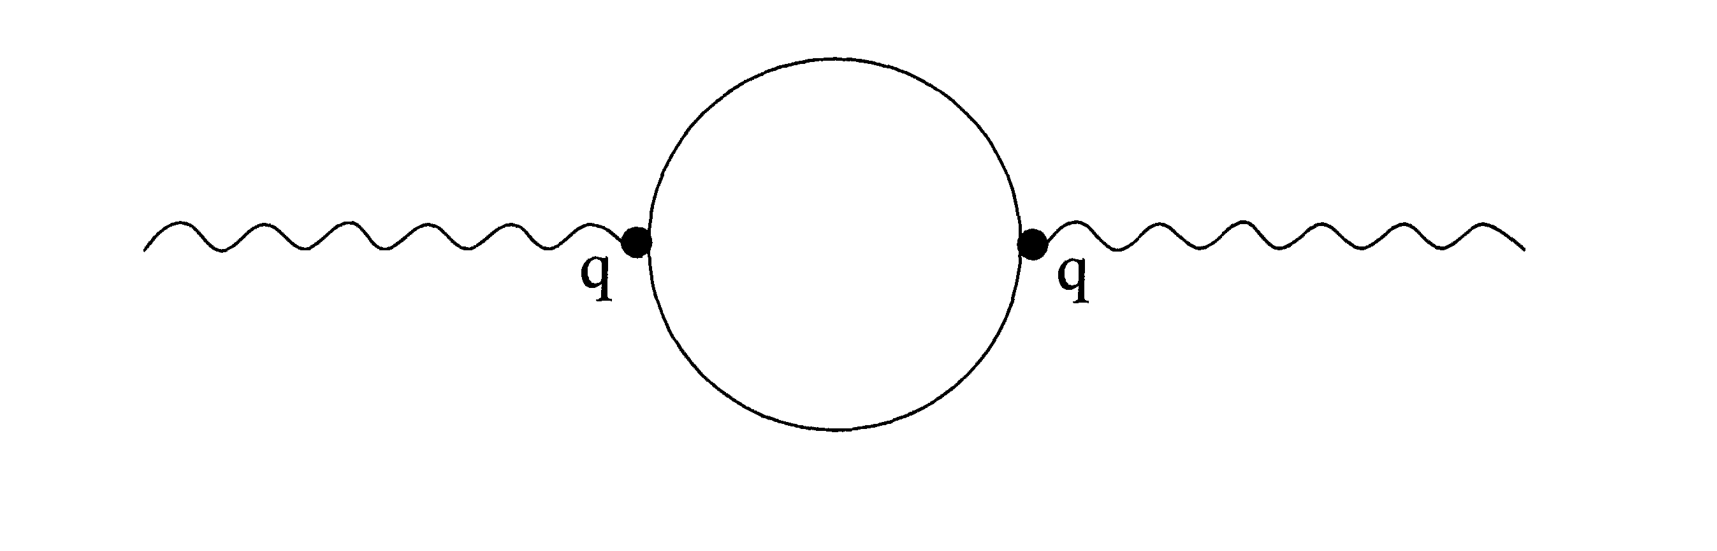
\includegraphics[width=0.62\textwidth]{figs/fig_p254_1.png}
  \caption{规范场（波浪线）经由超多重态（实线）圈的单圈自能图，两侧顶点均标记为荷 $q$。（原文 p.254 的插图，该页未标 Figure 号，此为第 1 张图。）}
  \label{fig:p254-1}
\end{figure}

（实线代表超多重态，波浪线代表矢量多重态。）这张图重整化规范场的动能项；重整化因子是 $u-u_0$ 的函数（因为超多重态的质量正比于 $|u-u_0|$），并且由于超多重态是无质量的，它在 $u\to u_0$ 时按对数发散。

结果是：对 $u$ 靠近 $u_0$ 的情形，我们有

\[
  \tau(u)=2q^2\,\frac{\ln(u-u_0)+\text{constant}}{2\pi i}.
\]

这意味着 $\tau(u)$ 在 $PSL(2,\mathbb{Z})$ 中绕这个奇点的单值变换（monodromy）是

\begin{equation}
  \tag{18.6}
  \label{eq:18-6}
  \pm\begin{pmatrix}1&2q^2\\0&1\end{pmatrix}.
\end{equation}

当然，单值变换实际上是 $SL(2,\mathbb{Z})$ 中的一个元素，由它在 $PSL(2,\mathbb{Z})$ 中的像只确定到相差一个符号。为了把这个符号定下来，我们作如下论证。$u=u_0$ 附近的物理由一个 $U(1)$ 规范理论描述，其规范场为 $(\tilde A,\tilde a)$，并带有一个在 $u_0$ 处变为无质量的带荷超多重态 $(T,\tilde T)$。因此，Lagrange 量具有规范耦合项再加上一个超势 $q\cdot\tilde aT\tilde T$ 的形式。标量场 $\tilde a$ 是 $u$ 平面上的一个局部坐标，而事实上它通过一个 $ISL(2,\mathbb{Z})$ 变换与无穷远处的 $a,a_D$ 相联系。（这个变换在 $SL(2,\mathbb{Z})$ 中的像，由超多重态 $(T,\tilde T)$ 相对于 $u$ 平面中无穷远处那个 $U(1)$ 的荷 $(n_e,n_m)$ 决定。）由于这个 $U(1)$ 理论在整个这个邻域中（甚至在奇点处）都存在，我们看到：在绕 $u_0$ 的单值变换下，场 $\tilde a$ 回到它自身。这意味着在绕 $u_0$ 的 $SL(2,\mathbb{Z})$ 单值变换下存在一个不变向量，从而表明单值变换正是方程 18.6 所写的那样，并且取正号。

% [Tutor Note: 「存在不变向量」这一步是定符号的关键，但作者没有说明它作用在哪一个向量空间上。准确的说法是：矩阵 $\pm\begin{pmatrix}1&2q^2\\0&1\end{pmatrix}$ 的迹是 $\pm2$；而"$\tilde a$ 原样返回"意味着在以 $(\tilde a_D,\tilde a)$ 为基的表示中，该矩阵的本征值必须是 $+1$（而不是 $-1$），故只能取迹为 $+2$ 的那个符号——整体负号会把本征值从 $(1,1)$ 变成 $(-1,-1)$，不变向量随之消失。另有一个极易出错之处：写成 $\begin{pmatrix}1&2q^2\\0&1\end{pmatrix}$ 时，必须明确它作用在列向量 $(\tilde a_D,\tilde a)^T$ 上（于是 $\tilde a_D\mapsto\tilde a_D+2q^2\tilde a$、$\tilde a\mapsto\tilde a$，即 $\tau\to\tau+2q^2$）；若改用 $(\tilde a,\tilde a_D)^T$ 的次序，$2q^2$ 就应挪到左下角。把次序与符号弄混，会得到 $\tau\to\tau-2q^2$ 从而与 $u$ 平面绕无穷远的 $\tau\to\tau-2$（见 (18.2) 与 (18.3)）在方向上讲不通。]

% [Tutor Note: $\ln(u-u_0)+\text{constant}$ 在量纲上并不合法：对数的宗量必须无量纲，而 $u$ 的量纲是质量的平方。规范写法是 $\ln\frac{u-u_0}{\mu^2}$（$\mu$ 为重整化标度），所谓 "constant" 实际上是 $-\ln\mu^2$ 再加上一个有限常数。这不是排印错误而是习惯写法，但它牵动两件事：(i) 常数项若取虚部，等于重新定义 $\theta$ 角，属于允许的重定义；(ii) 关键在于必须写 $\ln(u-u_0)$ 而不是 $\ln|u-u_0|$——只有前者在绕 $u_0$ 一周时给出 $\ln\to\ln+2\pi i$，从而 $\tau\to\tau+2q^2$，这正是 (18.6) 的来源；写成绝对值就得不到任何单值变换。同理，下面对多个超多重态求和时，每一项的对数分支必须取同一套，否则单值矩阵就不再是 $\begin{pmatrix}1&\sum_i2q_i^2\\0&1\end{pmatrix}$。]

我们可以把这一图像加以推广。假定在 $u_0$ 处有若干个荷为 $q_i$ 的超多重态变为无质量。那么 $\tau$ 的局部形式将是

\[
  \tau=2\sum_i q_i^2\,\frac{\ln(u-u_0)+\text{constant}}{2\pi i}.
\]

% ===== 原文 p.255 =====
而绕 $u_0$ 的单值变换将是

\[
  \begin{pmatrix}1&\sum_i2q_i^2\\0&1\end{pmatrix}.
\]

注意：在一个超多重态正在变为无质量的奇点处，单值变换的迹为 $2$，而无穷远处的单值变换的迹为 $-2$。特别地，这意味着：如果奇点来自无质量的超多重态，那么 $u$ 平面上不可能只有一个奇点。（由奇点之外 $\operatorname{Im}\tau$ 的正性，无论如何都可推出单值群必定是非阿贝尔的，因而奇点不止一个。）

\subsection{$\mathcal{M}$ 中奇点的数目}
% 原文 §18.5：The number of singularities in $\mathcal{M}$

为了理解 $\mathcal{M}$ 中奇点的数目，让我们从微观的 $\mathcal{N}=2$ 超对称 $SU(2)$ 理论出发，通过加上如下形式的微扰把它破缺为一个 $\mathcal{N}=1$ 超对称理论：

\begin{equation}
  \tag{18.7}
  \label{eq:18-7}
  \Delta\mathcal{L}=\int d^4x\,d^2\theta\,mu+\text{c.c},
\end{equation}

其中 $m$ 是复常数。（回忆 $u=\operatorname{Tr}\phi^2$。）正如第 16 讲以及 [II-N=1 Dynamics, §2.2] 中所讨论的，这个理论有两个真空，每一个都有质量间隙（mass gap）并且有禁闭（confinement）。

让我们假定，在量子真空空间的某一点处，有 $t$ 个超多重态变为无质量，比如说荷为 $q_i$ 的 $(T_i,\tilde T_i)$。于是在这点附近，物理由一个超势

\[
  W=\tilde a\Bigl(\sum_i q_iT_iT_i'\Bigr)+mu(\tilde a)
\]

描述，其中和以前一样，$\tilde a$ 是 $u$ 平面上的一个局部参数，并通过一个 $SL(2,\mathbb{Z})$ 变换与无穷远处的 $a,a_D$ 相联系。让我们求出宏观理论中的真空空间。也就是说，我们解出 $dW=0$ 并除以 $\mathbb{C}^*$ 作用。显然，方程 $dW=0$ 等价于

\[
  \tilde aT_i=\tilde aT_i'=0\qquad\text{对一切 }i,
\]

\[
  m\frac{du}{d\tilde a}+\sum_{i=1}^{t}q_iT_i\tilde T_i=0.
\]

若 $t>0$，这就给出一个正维数的真空空间。这是不可能的，因为微观理论只有两个真空。这意味着，在每个奇点处都只有一个超多重态变为无质量。其次，由于 $\frac{du}{d\tilde a}\neq0$，我们从第二个方程看出：当 $m\neq0$ 时，一个真空态满足 $T,\tilde T\neq0$。由第一个方程，这意味着 $\tilde a=0$。由于只有一个超多重态，方程变成

\[
  m\frac{du}{d\tilde a}\Big|_{\tilde a=0}+qT\tilde T=0.
\]

这确定了 $T\tilde T$，于是它在 $\mathbb{C}^*$ 作用之下唯一地确定了真空。由此可见，与这个奇点相联系的是一个唯一的真空。

% [Tutor Note: 这里 $T_iT_i'$ 的撇号与同一句中的 $(T_i,\tilde T_i)$ 记号不一致，而紧接在后的第二个 F 项方程又写成 $q_iT_i\tilde T_i$，可见 $T_i'$ 应为 $\tilde T_i$ 的排印之误（或撇号只是权且表示第二个分量）。译文照原样保留 $T_i'$，读者读作 $\tilde T_i$ 即可。另一处被跳过的是"解 $dW=0$ 并除以 $\mathbb{C}^*$ 作用"：在 $\mathcal{N}=1$ 语言中，真空应由 F 项方程 $\partial W/\partial\phi=0$ 与 D 项方程共同决定，再商去复化规范群；此处 $W$ 对 $T_i,\tilde T_i$ 是双线性的、对 $\tilde a$ 是线性的，D 项方程（形如 $\sum_iq_i(|T_i|^2-|\tilde T_i|^2)=0$）总可以沿 $\mathbb{C}^*$ 轨道取到满足，故真空模空间恰为 $\{dW=0\}/\mathbb{C}^*$。这是 Affleck--Dine--Seiberg 关于平直方向（flat direction）的标准论证，可参 Wess--Bagger《Supersymmetry and Supergravity》有关 F/D 平坦性的章节。]

% [Tutor Note: "若 $t>0$ 就得到正维数的真空空间"一句，靠的是：当 $t\geq2$ 时 $\tilde a=0$ 与 $\sum_iq_iT_i\tilde T_i=0$ 只给出一条方程，其余 $2t-1$ 个复方向都是平直的；商去 $\mathbb{C}^*$ 之后仍有 $2t-2>0$ 维，与"微观理论只有两个真空"直接矛盾。这一条正是本节数奇点的全部力量所在，它把 $t$ 硬压到 $1$，从而"一个奇点对应一个真空"。注意 $t=1$ 时方程 $\tilde aT=\tilde a\tilde T=0$ 与 $m\,du/d\tilde a+qT\tilde T=0$ 联立后给出 $\tilde a=0$ 与 $T\tilde T=-m\,du/d\tilde a|_{\tilde a=0}/q$，后者只定出乘积，剩下的相位被 $\mathbb{C}^*$ 吃掉——所以说"唯一确定"。作者没有提 D 项，理由同上一条批注。]

% ===== 原文 p.256 =====
宏观理论中每个奇点有一个真空，而微观理论只有两个真空，由此推出 $\mathcal{M}$ 中至多有两个奇点。于是我们看到

\[
  N_h\le2,
\]

其中 $N_h$ 是超多重态变为无质量的那些点的数目。

正如我们已经注意到的，绕一个超多重态无质量之点的单值变换，与无穷远处的单值变换的迹相反，因而它们在 $SL(2,\mathbb{Z})$ 中不是共轭的。所以根据这一点（或者因为我们需要非阿贝尔的单值群才能得到 $\operatorname{Im}\tau>0$），至少必须有两个超多重态变为无质量之点；也就是说 $N_h\ge2$。于是我们得出结论：$N_h=2$。

这样，尽管我们发现 $\mathcal{M}$ 与经典的真空模空间相同，二者却有重要的差别。经典地，$u$ 平面上只有一个奇点；在那里一个非阿贝尔规范群被恢复，但单值变换是阿贝尔的。量子力学地，$u$ 平面有两个奇点；单值变换是非阿贝尔的，但人们在长距离上永远不会遇到未破缺的非阿贝尔规范对称群。量子理论的非阿贝尔单值变换意味着：与经典情形不同，量子真空空间之上的那族环面并不具有常数 $j$ 不变量。这一点从关于 $u=\infty$ 附近行为的渐近公式 (18.2) 就已经清楚了。

到目前为止，我们已经在 $u$ 平面上找到两个奇点，当我们加上方程 18.7 中的微扰时，每个奇点贡献一个真空。既然受微扰的理论中至多有两个真空，由此推出：原来的 $\mathcal{N}=2$ 理论的量子真空空间不可能含有孤立点；因为那些孤立点也会产生受微扰理论的量子真空。这就补上了我们 §18.2 中把 $\mathcal{M}$ 等同于 $u$ 平面这一论证的一处缺口。

我们回忆：量子力学地，经典 Lagrange 量的 $U(1)_R$ 对称性被破缺为 $\mathbb{Z}/8\mathbb{Z}$ 对称性。由于 $u$ 在 $U(1)_R$ 之下荷为四，这个对称性在 $u$ 平面上作为一个 $\mathbb{Z}/2\mathbb{Z}$ 对称性作用。它就是对称性 $u\mapsto-u$。$\mathcal{M}$ 中的两个奇点必须构成一个 $\mathbb{Z}/2\mathbb{Z}$ 轨道，所以它们是点 $\pm u_0$，其中 $u_0\neq0$。正如我们已经看到的，量纲分析告诉我们 $u$ 的量级为 $\Lambda^2$，即理论中质量参数的平方。这意味着我们可以这样选取质量参数 $\Lambda$：使以 $\Lambda$ 标记的量子理论恰好在 $u=\pm\Lambda^2$ 处有奇点。这样我们就采用了引言中所许诺的质量标度参数 $\Lambda$ 的精确定义。注意这个 $\Lambda$ 的选取与我们此前一直使用的选取不同。这一改变的唯一效果，不过是改变公式 18.1 至 18.5 中的常数。

\subsection{新的无质量粒子}
% 原文 §18.6：The new massless particles

下一步是确定究竟是什么在变为无质量。设在一个使无穷远处的单值变换为上三角的基中，在 $\Lambda^2$ 处变为无质量的超多重态的荷为 $(n_e,n_m)$。若 $n_m=0$，则 $\Lambda^2$ 处的单值变换与无穷远处的单值变换对易。由于该族非奇异部分的全空间（total space）是三孔球面，$\Lambda^2$ 处与 $\infty$ 处的单值变换生成整个单值像。于是，如果 $\infty$ 处与 $\Lambda^2$ 处的单值变换同时为上三角，那么整个单值像都是上三角的，从而是可交换的。这将意味着 $\operatorname{Im}\tau$ 不可能处处为正。我们的结论是 $n_m\neq0$。也就是说，这个粒子……

% [Tutor Note: "该族非奇异部分的全空间（total space）是三孔球面"一语按字面读，维数就不对：族的全空间是椭圆纤维化的复曲面（复维数二），而只有底空间——即 $u$ 平面去掉 $+\Lambda^2,-\Lambda^2,\infty$ 三点，也就是 $\mathbb{CP}^1$ 去掉三点——才是三孔球面。此处 total space 应读作"底空间（base）"。这一点关系到下一句的逻辑：单值表示是底空间基本群的表示，而三孔球面的 $\pi_1$ 是秩二的自由群（绕其中两个 puncture 的圈即可生成，第三个是二者的乘积），所以"$\Lambda^2$ 处与 $\infty$ 处的单值变换生成整个单值像"才成立；若真按全空间理解，基本群还要多出纤维（环面）的两条圈，结论就不对了。]

% ===== 原文 p.257 =====
……在 $u=\Lambda^2$ 处变为无质量，因而带磁荷。对 $-\Lambda^2$ 处的奇点，完全相同的分析成立。这是一个非常有趣的现象。那些在 $|u|\gg\Lambda^2$ 时作为有质量孤子而开始其生命的粒子，随着 $u$ 趋近 $\pm\Lambda^2$ 而变为无质量。这也意味着，我们把 $\pm\Lambda^2$ 附近的理论描述为一个 $U(1)$ 理论，与 $u$ 平面中无穷远附近理论的 $U(1)$ 表示是不同的表示。

现在我们要计算这些粒子的磁荷 $\pm n_m$。注意：当我们从无穷远走入时，$\pm n_m$ 是良定义的，与我们从无穷远到 $\pm\Lambda^2$ 所选取的路径无关；但电荷却依赖于路径——如果我们绕这一对奇点转一圈，$\pm n_e$ 会改变两倍的磁荷，因为绕无穷远的单值变换是 $n_e\mapsto-n_e+2n_m$。$u=\infty$ 附近的磁单极子有 $n_m=\pm1$。这强烈地提示：在奇点处变为无质量的超多重态有 $n_m=\pm1$；这是一个重要的论断，我们将在 §18.7 中更精确地论证它。

我们今天讨论的这个模型有各种数学应用，但仅就物理而言，它最引人注目的应用之一是给出了一个关于禁闭的新模型。我们回忆：禁闭是指外加电荷之间存在线性势，或者等价地，在适当的表示中 Wilson 圈按面积律（area law）衰减（在目前的例子中，$SU(2)$ 的二维表示是个好选择）。我们从第 10 讲 §10.3 回忆起，在 Higgs 相中，当一个带荷场获得真空期望值\footnote{这是一个多少不够精确的描述，正如我们在前面几讲中所见，但在弱耦合下是成立的。}时，人们可以用一个拓扑论证显式地算出 't Hooft 圈按面积律衰减。如果人们能够天真地交换电与磁，那么 Wilson 圈就会与 't Hooft 圈互换，我们就会得出结论：一旦一个带磁荷的场获得真空期望值，禁闭就会出现。1970 年代 't Hooft、Mandelstam、Nambu 等人曾以启发性的方式论证过这一点，但在给出实际模型方面困难极大；因为在这个形式体系中通常并没有带磁荷的场，而带磁荷的客体（它们作为经典解出现）在弱耦合区域——正是在那里人们才能具体地理解它们——是很重的。因此，一般很难看出究竟怎样才能真正展示出一个带磁荷的场获得真空期望值的现象。

在目前的背景下，这件事发生了。我们已经看到，在把 $mu$ 微扰加到超势上之后（这一微扰预期给出禁闭），$u=\Lambda^2$ 附近的真空具有非零的超多重态场 $T,\tilde T$；所以在事实上，在这个真空中（$n_m$ 非零）一个带磁荷的客体已经获得了真空期望值。于是，正如所预期的，恰好在禁闭的情形中一个带磁荷的场获得了真空期望值。为了更精确地追踪这一点，所讨论的带磁荷的场具有奇数 $n_m$ 是重要的。的确，由于 $SU(2)$ 的中心是 $\mathbb{Z}/2\mathbb{Z}$，通过通常 Higgs 机制的对偶来解释禁闭，要求奇 $n_m$ 的场具有非零的期望值。$T$ 与 $\tilde T$ 实际上有奇数的 $n_m$，事实上就是 $\pm1$，正如我们上面以启发性的方式所论证、并将在 §18.7 中更精确地论证的那样。

已经发生的令人惊讶的事情之一是下面这件事。磁单极子在无穷远处的质量量级为 $\sqrt{|u|}\ln(|u|)$，而另外还有一些质量量级为 $\sqrt{|u|}$ 的 BPS 态。因此在无穷远处，磁单极子并不是……

% [Tutor Note: 这一段是全书最值得停下来想的一处对照。作者先说"如果能够天真地交换电与磁"——请注意这只是形式上的互换，不是任何对称性：电、磁的耦合常数互为倒数，弱耦合的磁图像正对应强耦合的电图像，所以这条推理只能算启发式的。真正的定量条件是：禁闭是关于 $SU(2)$ 的中心 $\mathbb{Z}/2\mathbb{Z}$ 的陈述（基本表示的 Wilson 圈只依赖 $n_e\bmod2$），对偶的 Higgs 机制要"探测"到这个中心，凝聚的磁荷就必须是奇数，$n_m\equiv1\pmod2$；若 $n_m$ 为偶数，凝聚对中心是"透明"的，磁通管可以被屏蔽，得不到面积律。另请注意"通常并没有带磁荷的场"这句话的准确含义：拉格朗日量里没有基本场携带 $n_m\neq0$，磁荷只能作为经典解（孤子）出现，因此磁荷凝聚必然是**非微扰**效应——这正是本模型在 1994 年显得惊人的原因。最后，"第 10 讲 §10.3"这一处引文在原文中印作 "Lecture 10.3"，与 p.260 参考文献里"第 10 讲"的说法对照，应读作第 10 讲的 §10.3（即该讲第 3 节），而不是"第 10.3 讲"。]

% ===== 原文 p.258 =====
……有质量粒子中最轻的。然而，在奇点处变为无质量的恰恰就是它们。在这一段里，我们实际上跑到了故事的前面，假定了在奇点处变为无质量的粒子，就是人们在大的 $|u|$ 处半经典地看到的那些 BPS 磁单极子。

\subsection{椭圆曲线族的显式性质}
% 原文 §18.7：Explicit nature of the family of elliptic curves

现在我们准备把各部分拼起来并求解这个模型。我们将显式地描述与本理论量子真空空间相联系的椭圆曲线族以及二形式 $\eta$。正如我们已经看到的，对这个理论而言，量子真空的模空间是 $\mathbb{C}$，参数为 $u=\operatorname{Tr}\phi^2$。该族在无穷远处的 $SL(2,\mathbb{Z})$ 单值变换是

\[
  \begin{pmatrix}-1&2\\0&-1\end{pmatrix}.
\]

此外，$u$ 平面上还有另外两个奇点 $\pm\Lambda^2$。在每个这样的点处，$SL(2,\mathbb{Z})$ 单值变换 $m_{\pm\Lambda^2}$ 的迹为二。我们写

\[
  m_{\Lambda^2}^{-1}=\begin{pmatrix}1+b&-b^2/a\\ a&1-b\end{pmatrix},
\]

其中 $a,b$ 为整数。（这是迹为二、行列式为一的矩阵的一般形式。）由于

\[
  m_{-\Lambda^2}=m_{\Lambda^2}^{-1}m_\infty
\]

的迹为二，我们推出

\[
  2=\operatorname{Tr}\begin{pmatrix}1+b&-b^2/a\\ a&1-b\end{pmatrix}\begin{pmatrix}-1&2\\0&-1\end{pmatrix}.
\]

由直接计算可得 $a=2$。由于 $-b^2/a$ 是整数，我们看到 $b$ 是偶数。现在让我们用矩阵

\[
  \begin{pmatrix}1&1\\0&1\end{pmatrix}
\]

来共轭 $m_{\Lambda^2}^{-1}$ 的矩阵，这个矩阵与无穷远处的单值变换对易。其效果是把 $b$ 改变 $2$。于是，经过若干次这样的共轭之后，我们到达 $b=0$。这意味着，在适当的基下，无穷远处的单值变换是

\[
  \begin{pmatrix}-1&2\\0&-1\end{pmatrix},
\]

而在 $\Lambda^2$ 处的单值变换具有形式

\[
  \begin{pmatrix}1&0\\-2&1\end{pmatrix}.
\]

这样，我们就证明了单值表示在 $SL(2,\mathbb{Z})$ 中唯一地确定到共轭。还要注意，按照方程 18.6，为了得到这个单值变换，在 $\Lambda^2$ 处变为无质量的超多重态的磁荷 $n_m$ 是 $\pm1$。当然，在 $-\Lambda^2$ 处同样成立。事实上，由于 $SL(2,\mathbb{Z})$ 表示唯一地确定到共轭，它在对称性 $u\mapsto-u$ 之下（在共轭的意义下）是不变的。

很容易识别出在上述单值变换下、两度穿孔平面之上的椭圆曲线族。该族的底空间可以等同于模曲线 $\mathbb{H}/\Gamma(2)$，它由把上半平面除以……

% [Tutor Note: "由直接计算可得 $a=2$"这一步值得完整写出，它是本页唯一的硬计算。把两矩阵相乘：$(1,1)$ 元为 $(1+b)(-1)+(-b^2/a)\cdot0=-1-b$；$(1,2)$ 元为 $(1+b)\cdot2+(-b^2/a)(-1)=2+2b+b^2/a$；$(2,1)$ 元为 $a\cdot(-1)+(1-b)\cdot0=-a$；$(2,2)$ 元为 $a\cdot2+(1-b)(-1)=2a-1+b$。故迹为 $(-1-b)+(2a-1+b)=2a-2$，令其等于 $2$ 即得 $a=2$——注意 $b$ 恰好消掉，这正是这个 ansatz 的用意。随后"$b$ 是偶数"用的是 $-b^2/a=-b^2/2\in\mathbb{Z}\Rightarrow b^2$ 偶 $\Rightarrow b$ 偶。最后一步共轭之所以"只改变 $b$ 而不改变 $m_\infty$"，是因为 $\begin{pmatrix}1&1\\0&1\end{pmatrix}$ 与 $m_\infty=\begin{pmatrix}-1&2\\0&-1\end{pmatrix}$ 对易（后者等于 $-T^{-2}$，与 $T$ 生成同一个抛物子群）；若误用 $\begin{pmatrix}1&0\\1&1\end{pmatrix}$ 之类不同矩阵去共轭，$m_\infty$ 会变形，整个论证就失效了。]

% [Tutor Note: 顺带验证一下记号的自洽性：形如 $M(a,b)=\begin{pmatrix}1+b&-b^2/a\\a&1-b\end{pmatrix}$ 的矩阵行列式恒为 $(1+b)(1-b)+b^2=1$，其逆为 $\begin{pmatrix}1-b&b^2/a\\-a&1+b\end{pmatrix}=M(-a,-b)$，仍属同一族。所以作者把 $m_{\Lambda^2}^{-1}$ 而非 $m_{\Lambda^2}$ 写成这个一般形，在迹方程里并不引入额外内容（$a\to-a$、$b\to-b$ 不过是重新命名整数参数）；真正要紧的是 $m_{-\Lambda^2}=m_{\Lambda^2}^{-1}m_\infty$ 中两个因子的次序，它由基的选取（先绕 $\Lambda^2$、再绕 $\infty$ 的合成顺序）决定——两个抛物元不交换，把次序颠倒通常会得到另一个解。判断次序是否正确的办法：解出的矩阵必须与 (18.6) 的 $\begin{pmatrix}1&2q^2\\0&1\end{pmatrix}$（$q=\pm1$）共轭，也就是迹为 $+2$ 且与 $m_\infty$ 一起生成非阿贝尔群；若解出的 $m_{\Lambda^2}$ 迹为 $-2$，说明次序或符号搞反了。]

% ===== 原文 p.259 =====
……$PSL(2,\mathbb{Z})$ 中由所有模二同余于恒等元的矩阵构成的子群的（自由）作用而得到。该族就是这个底空间上具有"二阶结构"（level two structure）的椭圆曲线万有族（universal family）。由于奇点在 $u=\pm\Lambda^2$ 处，与这个量子理论相联系的椭圆曲线族的 Weierstrass 方程是

\[
  y^2=(x-u)(x-\Lambda^2)(x+\Lambda^2).
\]

现在让我们考虑上一讲中所描述的二形式 $\eta$。我们知道，在上面给出的 Weierstrass 模型中，$\eta$ 具有一般形式

\[
  \eta=f(u)\,du\,\frac{dx}{y}.
\]

隐含地，在以前的讨论中我们假定了 $\eta$ 是一个没有零点与极点的复辛形式，至少远离 $u$ 的例外值。这样的零点或极点会产生非物理的奇点。如果我们取 $f$ 为非零常数，那么 Kähler 形式 $\pi_*(\eta\wedge\bar\eta)$ 除在 $\infty,\pm\Lambda^2$ 之外是光滑的，而在那里它具有正确的奇异行为。任何别的 $f$ 都会在别处产生极点或零点，或者在 $\infty,\pm\Lambda^2$ 之一处产生错误的奇异行为。由此推出：对某个适当的常数 $C$ 有 $\eta=C\,du\,\frac{dx}{y}$；这个常数可以通过与 $u=\infty$ 附近 $a^2=u$ 的公式相比较而算出。

显然，

\[
  \eta=d\Bigl(C\frac{u\,dx}{y}\Bigr)=d\Bigl(C\frac{2y\,dx}{x^2-\Lambda^4}\Bigr).
\]

形式 $\lambda=2Cy\,dx/(x^2-\Lambda^4)$ 是椭圆曲线族全空间 $\mathcal{E}$ 上的一个第二类微分（differential of the second kind）。这意味着——正如我们一直所断言的那样——$[\eta]\in H^2(\mathcal{E};\mathbb{C})$ 是平凡的，从而我们这个理论表示族的单值变换包含在 $SL(2,\mathbb{Z})$ 之中，即在更大的群 $ISL(2,\mathbb{Z})$ 之内。这是意料之中的，因为除了 $n_e,n_m$ 之外这个理论没有守恒荷。

% [Tutor Note: 这一串等号值得自己验算，因为"$[\eta]=0$"这一结论完全压在它上面。在总空间上以 $(u,x)$ 为局部坐标（$y$ 由 $y^2=(x-u)(x^2-\Lambda^4)$ 决定，故 $y_u=-(x^2-\Lambda^4)/(2y)$，从而 $d(dx/y)=d(1/y)\wedge dx=-y_u\,du\wedge dx/y^2$），有
% $d\bigl(u\frac{dx}{y}\bigr)=\frac{du\wedge dx}{y}\Bigl[1+\frac{u(x^2-\Lambda^4)}{2y^2}\Bigr]=\frac{2x-u}{2(x-u)}\cdot\frac{du\wedge dx}{y}$，
% 一般不等于 $\eta=C\,du\wedge dx/y$；而
% $d\bigl(\frac{2y\,dx}{x^2-\Lambda^4}\bigr)=\frac{2y_u\,du\wedge dx}{x^2-\Lambda^4}=-\frac{du\wedge dx}{y}$，
% 与 $\eta$ 只差一个整体符号（可并入常数 $C$ 的符号，或等价地把 $\lambda$ 定义为 $-2Cy\,dx/(x^2-\Lambda^4)$）。所以印刷的这条链式等式里，第二个等号只差符号（无害），第一个等号则差一个依赖 $u,x$ 的因子 $\frac{2x-u}{2(x-u)}$（例如在 $x=3,\ \Lambda=1,\ y=2$ 处该因子为 $7/2$），疑为笔误。幸而"$\eta$ 恰当、从而 $[\eta]=0$"只需第二个等号（至多差符号），结论不受影响。引用时请以显式计算为准。]
%
% [Tutor Note: "第二类微分"与"$[\eta]$ 平凡"之间的推理容易被误读成后者是前者的定义性推论。准确的说法是：第二类微分指留数全为零的亚纯微分；留数为零保证 $\lambda$ 沿围绕任何极点的闭路积分不产生 $2\pi i$ 型的多值性，于是 $\lambda$ 是 $\mathcal{E}$ 上单值良定义的 $1$-形式，$\eta=d\lambda$ 便是整体恰当的，这才给出 $[\eta]=0\in H^2(\mathcal{E};\mathbb{C})$，并且 $\eta$ 沿闭链的周期可由 $\lambda$ 的周期直接读出（这正是确定 $a,a_D$ 的基础）。反之，若 $\lambda$ 在某处有非零留数（例如沿一条退化纤维），$\eta$ 就只能在该除子的补集上恰当，$[\eta]\neq0$，单值群便会落在 $ISL(2,\mathbb{Z})$ 而不在 $SL(2,\mathbb{Z})$ 中——这正是作者紧接着要排除的情形。]

\subsection{BPS 谱的描述}
% 原文 §18.8：Description of the BPS spectrum

通过对我们已经找到的椭圆曲线族作进一步研究，可以证明：$u$ 平面中 $a/a_D$ 为实的曲线是一条简单闭曲线，它经过点 $u=\pm\Lambda^2$，并且与实 $u$ 轴再无其他交点。在这条闭曲线之外，BPS 谱是连续的。从 $u=\infty$ 出发趋近，我们看到在 $u=\Lambda^2$ 处有 $a_D=0$ 而 $a\neq0$，而在 $u=-\Lambda^2$ 处有 $-a+a_D=0$ 而 $a\neq0$。（当然，确切的值依赖于从 $\infty$ 到 $\pm\Lambda^2$ 所选的路径，但如果我们沿正实轴或负实轴从无穷远走入，上述方程成立。）由于我们可以从无穷远趋近这两个奇点而不穿过 BPS 态的跳变轨迹（jumping locus），我们看到：在 $u=\pm\Lambda^2$ 处变为无质量的 BPS 态，确实就在无穷远处的原有 BPS 态之中。也就是说，这些粒子是无穷远处原有磁单极子的解析延拓。这就证实了早先以不那么正式的方式所提示的东西。

现在让我们考察：在跳变轨迹上除 $\pm\Lambda^2$ 之外的其他点处，是否还有被迫变为无质量的粒子。当我们沿跳变线在从 $\Lambda^2$ 到 $-\Lambda^2$ 的开上半弧上移动时，我们发现对每个满足 $0<s<1$ 的 $s$，都存在一个使 $sa-a_D=0$ 的点。因此，如果在无穷远处有一个 BPS 态，其荷 $(n_e,n_m)$ 对某个 $t\in\mathbb{R}$ 满足 $(n_e,n_m)=t(s,-1)$，那么在……

% ===== 原文 p.260 =====
……这条开弧上的某一点处，我们发现这个态变为无质量。这一点，再加上对跳变线的开下半弧所作的对称论证，表明：无穷远处所有荷 $(n_e,n_m)$ 满足 $0\le|n_e|\le|n_m|$ 的 BPS 态，都在跳变曲线上某处变为无质量（这恰好发生在点 $u=\pm\Lambda^2$ 处，当且仅当 $n_e=0$ 或 $n_e=\pm n_m$）。通过在无穷远处作一次单值变换（对大的 $u$ 而言它是谱的对称性），任何 $n_m\neq0$ 的 BPS 态都可以映到某个满足 $|n_e|\le|n_m|$ 的态。所以，无穷远处每一个 $n_m\neq0$ 的 BPS 态，只要沿适当的围道从无穷远把它引进来，都会在跳变线上某处变为无质量。

由于跳变线上除对应于 $a_D=0$ 或 $a_D-a=0$ 的那些奇点之外没有别的奇点，而由于那些奇点只用一个变为无质量的超多重态来解释，我们得出结论：对大的 $u$ 而言，除了已纳入我们分析的那些 $n_m=\pm1$ 的态之外，没有 $n_m\neq0$ 的 BPS 态。

这个论断蕴涵着关于经典几何的如下陈述。设 $\mathcal{W}_k$ 是本理论 $k$ 单极子解的模空间，再除以平移与整体 $U(1)$ 旋转而约化。它是一个维数为 $4k-4$ 的超 Kähler（hyper-Kähler）流形，在数学上已被大量研究。可以证明：$\mathcal{W}_k$ 上的 $L^2$ 全纯形式（可能取值于一个平坦线丛（flat line bundle））会给出 $k$ 单极子束缚态，$k>1$。这样的束缚态会产生不想要的奇点，或者对奇点处的单值变换作出不想要的贡献，所以 $\mathcal{W}_k$ 上不应有 $L^2$ 全纯形式。更一般地，A. Sen 利用 $\mathcal{N}=4$ 超 Yang--Mills 理论的对偶性（而不是本讲所考虑的 $\mathcal{N}=2$ 理论）所作的一个论证，定出了 $\mathcal{W}_k$ 的完整 $L^2$ 上同调。

% [Tutor Note: "对每个 $s\in(0,1)$ 有 $sa-a_D=0$ 之点"与后文"$0\le|n_e|\le|n_m|$"之间的对应，本质是边缘稳定性（marginal stability）条件：中心荷为 $Z=n_ea+n_ma_D$，代入 $(n_e,n_m)=t(s,-1)$ 得 $Z=t(sa-a_D)$，故"该态在某点变为无质量"（$Z=0$）恰等价于该点满足 $sa=a_D$。$s$ 跑遍 $(0,1)$ 给出荷矢量的一个开锥；端点 $s=0$ 与 $s=1$ 分别对应 $n_e=0$ 与 $n_e=\pm n_m$，也就是奇点 $u=\pm\Lambda^2$ 所在的两个端点——这正是括号里那句"当且仅当"的来源。另注意原文此处印作 "all the BPS states at infinity that satisfy of charges $(n_e,n_m)$ with ..."，"satisfy of charges" 是明显的语病（应为 satisfy 或 have charges），译文按语义译出，不影响内容。]

\subsection{参考文献与交叉引用}
% 原文 References and cross references

正如标题所表明的，本讲建立在第 17 讲的基础之上；和以前一样，基本文献是

N. Seiberg and E. Witten, \emph{Electric--Magnetic duality, monopole condensation,
and confinement in $\mathcal{N}=2$ supersymmetric Yang--Mills theory},
Nucl. Phys. B \textbf{426} (1994), pp. 19--52.

关于 Sen 工作的文献是

A. Sen, \emph{Dyon--Monopole Bound States, Selfdual Harmonic Forms On The
Multi-Monopole Moduli Space, and $SL(2,\mathbb{Z})$ Invariance In String Theory},
Phys. Lett. \textbf{B329} (1994) pp. 217--221.

't Hooft 圈与禁闭在第 10 讲中讨论。单圈 $\beta$ 函数计算的讨论见第 16 讲 §2，也见 [I-Renorm Groups] 的第 2、3 讲以及 [II-CFT] 的第 3 讲。BPS 态在第 12 讲中有详细讨论。

% [Tutor Note: 文献代号 [I-Renorm Groups] 与 [II-CFT] 指本丛书第 I 卷的"重整化群"章与第 II 卷的"共形场论"章（参见本书文献代号表）；本讲的另一文献代号 [II-N=1 Dynamics]（见 p.255）指第 II 卷关于 $\mathcal{N}=1$ 动力学的那一章。这三处代号在原文中一律用方括号大写罗马数字标注，翻译时原样保留，切勿改成书名或页码。]


\clearpage
% 原文 pp.261–268（印刷 pp.1379–1386）

\section{Lecture 19：四维 $\mathcal{N}=2$ 超对称 Yang--Mills 理论（三）：拓扑应用}

\begin{keytakeaways}
本讲把前两讲在 Minkowski 四维空间上得到的 $\mathcal{N}=2$ 超对称 Yang--Mills 低能动力学，搬到一般的紧致定向 Riemann 四维流形 $X$ 上，为 Donaldson 不变量寻找 Seiberg--Witten 式的表述。
定性上的分水岭是单圈 $\beta$ 函数 $\beta_1(g)=-\frac{g^3}{8\pi^2}\bigl(4h-c_2(\rho)\bigr)$ 的符号：为负则理论渐近自由、是好的基本理论，为零则 $\beta\equiv0$、$\tau$ 是常数且理论具有 $\Gamma\subset SL(2,\mathbb{Z})$ 的对偶对称性，为正则理论在紫外不自由、只能充当红外极限的候选者。
数学工具是扭变（twisting）：把 $Spin(4)=SU(2)_+\times SU(2)_-$ 中的 $SU(2)_+$ 与 $\mathcal{N}=2$ 的 $R$ 对称性 $SU(2)_R$ 取对角，得到 $SU(2)'$，于是超对称生成元 $Q^i_\alpha$ 与 $\bar Q_{j\dot\alpha}$ 都落入 $Spin(4)$ 的矢量表示，从而可在任意定向 Riemann 四维流形 $X$ 上整体定义。
扭变的几何后果是：在分裂超流形 $\Lambda^0TX\oplus TX\oplus\Lambda^2_+(TX)$ 上存在一个处处非零的整体实向量场 $Q=\partial_{\mathbf{R}^{\rm odd}}+\theta^i\partial_{i,{\rm even}}$，满足 $Q^2=0$ 与 $\{Q,K\}=d$；而由 $\{Q,\mathcal{S}\}=T$ 可得 $\{Q,T\}=0$，故所关心的关联函数与度规无关。
主要结论是：由 Chern 形式与手征标量 $\phi$ 造出的 $Q$-闭算符 $\mathcal{O}_P^{(n)}=K^nP(\phi)$ 正是 Donaldson 类在此框架中的对应物，其期望值等于各拓扑类型的模空间 $\mathcal{M}_E$ 上 $\mu_P(\Sigma)$ 的杯积积分；而扭变之后矢量多重态的全部场都化为微分形式，因而在任意闭定向四维流形上都有定义。
\end{keytakeaways}

% ===== 原文 p.261 =====
% 原文标题页：LECTURE 19 / $N=2$ Super-symmetric Yang-Mills Theories in Dimension Four: Part 3, Topological Applications

\subsection{四维 $\mathcal{N}=2$ 超对称规范理论概览}
% 原文 §19.1：A survey of $N=2$ supersymmetric gauge theories in dimension four

让我们先对 $\mathcal{N}=2$ 超对称规范理论的各类情形作一简要概述\footnote{原文页脚：\emph{Notes by John Morgan}——本讲笔记由 John Morgan 整理。}。我们必须指定一个规范群 $G$，它将是一个紧致连通群。为得到 $\mathcal{N}=2$ 超对称，我们的场中包含一个矢量多重态（vector multiplet），它由规范场及其超伙伴场构成，取值于主 $G$-丛的伴随丛（adjoint bundle）。我们也可以有超多重态（hypermultiplet）。设 $n$ 为超多重态的数目。$n$ 个自由超多重态的全局对称群是辛群 $Sp(n)$（即 $n\times n$ 四元数矩阵构成的酉群）。以 $\mathcal{N}=2$ 不变的方式对理论作规范化（gauging），可以通过规范化 $Sp(n)$ 的任意所需子群来实现。因此一般而言，超多重态位于由表示 $\rho:G\to Sp(n)$ 与主 $G$-丛相伴的向量丛中。

对理论的定性性质而言最重要的不变量是 $\beta$ 函数，尤其是单圈 $\beta$ 函数。单圈 $\beta$ 函数的公式为
\[
\beta_1(g)=-\frac{g^3}{8\pi^2}\bigl(4h-c_2(\rho)\bigr),
\]
其中 $h$ 是群 $G$ 的对偶 Coxeter 数（dual Coxeter number），$c_2(\rho)$ 是表示 $\rho$ 的二次 Casimir 的迹，其归一化使得 $SU(2)$ 的定义表示具有 $c_2$ 等于一。当然，$2h$ 正是 $c_2(\text{adjoint})$，即 $G$ 的伴随表示在其李代数上的二次 Casimir。有三种可能性：
\begin{itemize}
\item 单圈 $\beta$ 函数为零。
\item 单圈 $\beta$ 函数为负。
\item 单圈 $\beta$ 函数为正。
\end{itemize}

% [Tutor Note: 此处 $c_2$ 的归一化是核对本讲一切公式的第一道关口。作者取「$SU(2)$ 定义表示的 $c_2$ 等于一」，即 $c_2(\rho)=2T(\rho)$（国内教材常用的指标 $T$ 以 $T(\text{fund})=1/2$ 归一化）；只有在这个约定下才有「$2h=c_2(\text{adjoint})$」，这也正是 $h$ 被称为\emph{对偶} Coxeter 数的原因。最容易出错的是括号里的 $4h$ 而非 $2h$：规范多重态贡献 $2c_2(\text{adj})$，而 $c_2(\text{adj})=2h$，故为 $4h$。可自行校验：下一页（p.262）说 $c_2(\rho)=4h$ 对应「伴随表示复化的两份」，而每份伴随的 $c_2$ 是 $2h$，两份恰为 $4h$——若把 $4h$ 误抄成 $2h$，这个 $\mathcal{N}=4$ 判据立刻失效，且纯 $SU(2)$ 的 $\beta_1$ 会差一个因子 $2$。]

由于
\[
\tau=\frac{\theta}{2\pi}+\frac{4\pi i}{g^2},
\]

% ===== 原文 p.262 =====
我们有展开
\[
\mu\frac{d}{d\mu}(\tau)=\text{constant}+\sum_{\ell\ge1}C\cdot g^{2\ell}+\sum c_{n,\ell}\,g^{2\ell}\exp(2\pi i n\tau),
\]
其中常数项由单圈 $\beta$ 函数算出，$g$ 的更高次幂来自更高圈的贡献，而指数项来自瞬子修正（instanton correction，它们在微扰论中当然是看不到的）。由超对称性，$\mu\frac{d}{d\mu}(\tau)$ 是全纯函数，因此该展开中 $g$ 的正幂次项恒为零。于是，若单圈 $\beta$ 函数为零，则 $\beta$ 在微扰论中为零。在这种情况下，人们相信 $\beta\equiv0$。这一点尚未被严格证明，但显然，当单圈 $\beta$ 函数为零时，我们在前两讲中分析过的那类低能有效场论，只有在 $\beta$ 函数恒等于零时才有意义。（相反，单圈 $\beta$ 函数非零的 $\mathcal{N}=2$ 理论确实有非微扰的瞬子修正，正如我们在纯 $SU(2)$ 理论中所见。）

% [Tutor Note: 「由超对称性 $\mu\frac{d}{d\mu}\tau$ 是全纯函数，故 $g$ 的正幂次项恒为零」这句跳过了关键一步：全纯性是就 $\tau$ 而言的（在 $\mathcal{N}=2$ 中 $\tau$ 是手征超场的 $F$ 项系数，重整化只允许它作全纯移动），而 $\tau$ 与 $g$ 的关系是 $g^2=4\pi i/(\tau-\theta/2\pi)$；把 $\mu\frac{d\tau}{d\mu}$ 写成 $g$ 的幂级数时，$\ell\ge1$ 的每一项都隐含 $\ln\Lambda$ 型的非全纯依赖，故必为零。换算关系本身值得记住并用来验算：由 $\tau$ 的定义直接求导得 $\mu\frac{d\tau}{d\mu}=-8\pi i\,g^{-3}\beta(g)$，代入 $\beta_1=-\frac{g^3}{8\pi^2}(4h-c_2(\rho))$ 得常数项 $i(4h-c_2(\rho))/\pi$；反之若把 $\tau$ 写成常见的 $\theta/2\pi+i/g^2$（少一个 $4$），这里就会整体差因子 $4$。另注：指数项中 $n$ 的求和未写范围，实为 $n\ge1$，且瞬子展开的收敛性要求 $\operatorname{Im}\tau>0$（即 $g^2>0$），这正是 $\tau$ 取上半平面的原因。]

$\mathcal{N}=2$ 理论中 $c_2(\rho)=4h$ 的一个重要特例，是超多重态表示 $\rho$ 为伴随表示复化的两份这一情形。\footnote{任一秩为 $n$ 的实表示 $W$——这里 $W$ 是伴随表示，$n$ 是群的维数——都可以看作 $SO(n)$ 中的一个表示。$W\otimes_{\mathbb{R}}\mathbb{C}$ 的两份可以看作辛群 $Sp(n)$ 中的一个表示。为简洁起见，我们将把「$W$ 的复化的两份」称作「$W$ 与四元数作（$\mathbb{R}$ 上的）张量积」，其中四元数就简单地理解为带非退化斜形式的 $\mathbb{C}^2$。} 这个理论实际上具有 $\mathcal{N}=4$ 超对称。利用这一增强的超对称性可以证明，$\beta$ 函数恒为零。

当 $\beta\equiv0$ 时，量子理论与经典理论一样具有一个定义良好的常数 $\tau$。人们相信，在这种情况下存在 $SL(2,\mathbb{Z})$ 中一个有限指数的子群 $\Gamma$，使得理论在 $\Gamma$ 的忠实作用下不变。当然，当 $\beta\ne0$ 时理论有质量标度，$\tau$ 不再是常数。对于这些理论，人们会预期（正如我们在前两讲中对纯 $SU(2)$ 理论所见）：理论并不存在精确的对偶对称性，反倒是各种可能的低能描述之间的对偶，对于理解低能物理十分重要。

当单圈 $\beta$ 函数为负时，$\beta$ 函数为负，至少对足够高的能标如此。（我们上次研究的纯 $SU(2)$ 理论即属此类。）在这种情况下，我们有一个渐近自由（asymptotic freedom）的理论，它是一个好的基本理论。也就是说，我们有一个提法良好的\emph{问题}（即描述该理论的低能有效版本）。我们在上一讲中对 $G=SU(2)$ 或 $SO(3)$、$\rho$ 为平凡表示的情形解决了这个问题。

当单圈 $\beta$ 函数为正时，我们没有提法良好的问题，因为理论不是渐近自由的。毋宁说，这些理论是那些单圈 $\beta$ 函数为负的理论所提出的问题的候选解。更确切地说，一个 $\beta$ 函数为正的理论 $T_{\rm mac}$ 之所以是候选解，是因为它的低能有效理论提法良好且在红外自由。它是 $\beta$ 为负的理论 $T_{\rm mic}$ 所提问题的解，如果 $T_{\rm mic}$ 在红外流向 $T_{\rm mac}$，即在长距离（或等价地，低能量）下两个理论的关联函数相互收敛。把问题与答案配对、弄清楚哪些 $T_{\rm mac}$ 可以作为给定 $T_{\rm mic}$ 的红外极限出现，这个一般问题尚未解决，尽管在许多有趣的情形中已有大量结果。

% ===== 原文 p.263 =====
我们今天讨论的规范理论，是由量子化经典物理而得到的 Lagrange 模型。至少顺带一提：四维中还存在更为奇特的 $\mathcal{N}=2$ 理论，其中一些来自弦论。并非所有这些理论都有已知的 Lagrange 表述。无论它们是否有 Lagrange 量，这些 $\mathcal{N}=2$ 超对称理论在扭变之后也应当给出四维流形的不变量。那些没有 Lagrange 量的理论，可能给出这样的四维流形不变量：它们没有以某个微分方程之解的模空间为基础的经典描述。

\subsection{从 Minkowski 空间到紧致 Riemann 四维流形}
% 原文 §19.2：From Minkowski space to a compact Riemannian four-manifold

让我们固定一个 $\mathcal{N}=2$ 超对称渐近自由规范理论（即 $\beta<0$ 的那一个）。例如，若我们想研究 Donaldson 理论，就取纯 $\mathcal{N}=2$ 超对称 $SU(2)$ 规范理论。但在一段时间内，我们可以更一般些。到目前为止我们所讨论的理论，都位于 Minkowski 四维空间上。也就是说，我们写下的作用量涉及在 Minkowski 空间上对一个由该空间上各种场构成的 Lagrange 函数作积分。我们希望从它过渡到一个定义在紧致 Riemann 四维流形上的理论。这一过渡分两步完成——i) 从 Minkowski 四维空间转动到欧氏四维空间；ii) 整体化（globalize）到紧致 Riemann 四维流形。

让我们回忆去年秋天学到的、如何把理论 Wick 转动到欧氏四维空间。我们的理论由一族带有算符乘积展开（operator product expansion，O.P.E.）的局部算符构成。理论的一个实现（realization）给出这些算符在 Minkowski 四维空间各点处关联函数的值。但在 Minkowski 四维空间复化之后的一个开子集上，O.P.E. 与关联函数可由解析延拓定义。这个开子集包含欧氏四维空间。我们就是这样通过 Wick 转动把理论定义在欧氏四维空间上（例如见 [I-Axiomatics] 的第 2 讲）。在我们的情形中，所处理的是（超对称的）作用量
\[
S=\int_{M^4}\mathcal{L},
\]
它们是 Lagrange 量 $\mathcal{L}$ 的积分，而 $\mathcal{L}$ 是涉及底流形 Minkowski 空间上诸场 $\phi$ 的解析表达式。这些表达式延拓为复化 Minkowski 空间上的全纯表达式，然后可以限制到欧氏子空间上，产生欧氏 Lagrange 量 $\mathcal{L}_E$。欧氏作用量定义为
\[
S_E=\int_{\mathbb{R}^4}\mathcal{L}_E.
\]
Minkowski 空间中关联函数的路径积分为
\[
\int\mathcal{D}\phi\,\mathcal{O}_1(x_1)\cdots\mathcal{O}_t(x_t)\,e^{iS},
\]
而在这一过程中它 Wick 转动为路径积分
\[
\int\mathcal{D}\phi\,\mathcal{O}_1(x_1)\cdots\mathcal{O}_t(x_t)\,e^{-S_E},
\]

% ===== 原文 p.264 =====
计算的是欧氏空间中的关联函数。即使人们关心的是 Minkowski 空间，计算也常常在欧氏空间中进行，因为那里有一些技术上的简化。关于二者关系的更多细节，见 [I-Classical Fields] 第 7 章。

\subsubsection{通过扭变实现整体化——超对称代数情形}
% 原文 §19.2.1：Globalizing by twisting – the case of the supersymmetry algebra

现在让我们考察把该量子场论放到定向 Riemann 四维流形 $X$ 上的问题。我们的超对称理论是在四维空间上由一个作用量 $S$ 定义的，$S$ 是局部场的 Lagrange 函数的积分；这些场在 $Spin(4)$ 下按标量、旋量与矢量变换。当然，在 Minkowski 或欧氏四维空间上，有与这些表示相伴的丛。为了在四维流形 $X$ 上写下「同一个」作用量，我们需要能够在该流形上写下超对称 Lagrange 量。这意味着，Lagrange 量中出现的所有场都必须在 $X$ 上整体定义（作为丛的截面）。就目前所呈现的理论而言，一般情形下并非如此，因为相关的旋量丛可能不在 $X$ 上整体存在。事实上，Riemann 四维流形上的「物理」理论（即真正把理论与广义相对论耦合时会用到的那种）要求 $X$ 是 spin 流形，并且一般会破坏掉全部超对称。我们此前已经看到（第 14 讲 §3），对拓扑应用如何处理这个问题——我们用一个适当的同态把自旋群 $Spin(4)$ 映入 $R$ 对称群，以此扭变（twist）理论。我们将会看到，适当的扭变既使我们能在任意定向 Riemann 四维流形上写下 Lagrange 量，又使我们能保住超对称的一个关键部分。

把 $\Lambda^2T^*\mathbb{R}^4$ 分解为自对偶与反自对偶两部分，这由群 $Spin(4)$ 分解为 $SU(2)_+\times SU(2)_-$ 所覆盖。幸运的是，对 $\mathcal{N}=2$，$R$ 对称群是 $U(2)_R=SU(2)_R\times U(1)_R$。（$U(1)_R$ 常常并不存在，例如当超多重态有非零裸质量时；当 $\beta\ne0$ 时它也有反常。但即便如此，我们仍以 $SU(2)_R$ 作为 $R$ 对称群。）有了这个 $R$ 对称群，扭变才有可能，因为存在从 $Spin(4)$ 到 $SU(2)_R$ 的非平凡同态。（对 $\mathcal{N}=1$，$R$ 对称性是 $U(1)_R$，而在四维中不存在扭变的可能性。）回忆 [I-Supersolutions] 第 10 章：超对称生成元是 $\mathbb{R}^{4|8}$ 上的右不变向量场，记为 $Q^i_\alpha$ 与 $\bar Q_{j\dot\alpha}$，其中 $1\le i,j,\alpha\le2$。这两组生成元都在 $i,j$ 指标上按标准方式受 $SU(2)_R$ 作用。（$\alpha$ 与 $\dot\alpha$ 是 $SU(2)_+\times SU(2)_-$ 的旋量指标。）自旋群与 $SU(2)_R$ 的作用归纳在下表中。

\begin{center}
\begin{tabular}{|c||c|c|c|}
\hline
\multicolumn{1}{|c||}{} & \multicolumn{3}{c|}{各群下的变换}\\
\hline
\multicolumn{1}{|c||}{荷} & $SU(2)_+$ & $SU(2)_-$ & $SU(2)_R$\\
\hline
$Q^i_\alpha$ & $\frac12$ & $0$ & $\frac12$\\
\hline
$\bar Q_{j\dot\alpha}$ & $0$ & $\frac12$ & $\frac12$\\
\hline
\end{tabular}
\end{center}

% [Tutor Note: 这张表的指标位置是全书最容易抄错的地方之一。$Q^i_\alpha$ 的\emph{上}指标 $i$ 是 $SU(2)_R$ 的指标（$i=1,2$），\emph{下}指标 $\alpha$ 是 $SU(2)_+$ 的旋量指标；$\bar Q_{j\dot\alpha}$ 则相反：$j$ 在下、且带点的 $\dot\alpha$ 属于 $SU(2)_-$。扭变时被「吃掉」的正是 $i$ 与 $\alpha$ 这一对（对角化 $SU(2)_+$ 与 $SU(2)_R$），所以若把两者写反，下一页 $Q^i_\alpha$ 分解为 $(0,0)\oplus(1,0)$ 的结论会变成另一个表示，整个扭变就错了。另外，$SU(2)_-$ 的那一列对两个生成元分别给出 $0$ 与 $\frac12$，这恰是 $\bar Q$ 带点指标 $\dot\alpha$ 的体现——表中 $SU(2)_-$ 列非零的行正是 $\bar Q$ 所在的行。]

我们定义 $SU(2)'$ 为 $SU(2)_+\times SU(2)_R$ 在对这两个群的显然认同（identification）之下的对角子群。仍然在 $\mathbb{R}^4$ 上工作，我们将关心

% ===== 原文 p.265 =====
Poincaré 群的一个作用，其中通常的转动群 $Spin(4)$ 被 $SU(2)'\times SU(2)_-$ 取代。由表中的信息可以推出，在 $SU(2)'\times SU(2)_-$ 下，$Q^i_\alpha$ 按表示
\[
\Bigl(\frac12\otimes\frac12,0\Bigr)=(0,0)\oplus(1,0)
\]
变换。这意味着，$Q^i_\alpha$ 的扭变形式分解为一个复值向量场，与一个取值于复自对偶二形式的向量场。类似地，$\bar Q_{j\dot\alpha}$ 按同一群的表示
\[
\Bigl(\frac12,\frac12\Bigr)
\]
变换，从而是切向量，于是 $\bar Q_{j\dot\alpha}$ 成为取值于复化切丛的向量场。因此，这两个表示都是 $Spin(4)$ 的矢量表示，从而在任何定向 Riemann 四维流形上都整体存在。另外请注意，这些表示自然地是实表示（尽管原来的表示并不是）。这意味着在 Riemann 流形上我们可以取实场。

% [Tutor Note: 原文此处作「\emph{If} follows from the information in the table that…」，显系「\emph{It} follows…」之误（排印脱字），译文按正确读法处理。数学上这一步的实质是 $SU(2)$ 的张量积分解 $\frac12\otimes\frac12=0\oplus1$：$Q^i_\alpha$ 原本在 $SU(2)_+\times SU(2)_R$ 下按 $(\frac12,\frac12)$ 变换，对角化之后该表示限制为 $0\oplus1$，其中单态 $(0,0)$ 就是后来那个整体存在的标量型生成元 $Q$，三重态 $(1,0)$ 则给出取值于自对偶二形式的向量场；而 $\bar Q$ 的 $(\frac12,\frac12)$ 在对角化后仍是一个「矢量」，因为 $\frac12\otimes\frac12$ 中恰含一个自旋 $1$ 分量、且其 $SU(2)_-$ 指标 $\dot\alpha$ 保持不动（故为反自对偶侧）。]

用超空间的语言说，扭变并过渡到一般四维流形，意味着把超流形 $\mathbb{R}^{4|8}$（即 $\mathbb{R}^4$ 的超对称扩充）替换为一个分裂超流形（split supermanifold），其偶部是四维流形 $X$，奇部是宇称反转的向量丛 $\Lambda^0TX\oplus TX\oplus\Lambda^2_+(TX)$。在这个超流形上，我们有如下定义的一个整体实向量场 $Q$。设我们在 $X$ 的某个开子集上有局部坐标 $(x^1,\dots,x^4)$。令 $\theta^{\mathbf{R}}$ 为奇的 $\Lambda^0TX$ 方向上的自然坐标，$\theta^i$ 为由 $x^i$ 决定的奇的 $TX$ 方向上的坐标。我们以 $\partial_{\mathbf{R}^{\rm odd}}$ 与 $\partial_{i,{\rm odd}}$ 记这些奇方向上相应的向量场。最后，$\partial_{i,{\rm even}}$ 是沿 $x^i$ 方向的通常偏导数。我们写
\[
Q=\partial_{\mathbf{R}^{\rm odd}}+\theta^i\partial_{i,{\rm even}}.
\]
显然，当改变局部坐标时，这个表达式不变。这给出超流形上一个整体定义的实向量场 $Q$，它是局部超对称生成元 $Q^i_\alpha$ 的扭变形式的 $(0,0)$ 分量的整体化。正因为存在这样一个整体的、处处非零的、满足 $Q^2=0$ 的超对称生成元，我们才能在 $X$ 上做整体的拓扑量子场论。

我们还在 $X$ 上有一个整体定义的一形式 $K$，取值于超流形上的向量场。它由 $\bar Q_{j,\dot\alpha}$ 的扭变形式导出。在同一局部坐标下，它的公式是：
\[
K=\bigl(\partial_{i,{\rm odd}}+\theta^{\mathbf{R}}\partial_{i,{\rm even}}\bigr)\,dx^i.
\]
由公式可以直接看出，$K$ 在坐标变换下不变，从而是 $X$ 上一个定义良好的整体对象。

% [Tutor Note: 「显然，当改变局部坐标时这个表达式不变」是全书最需要停下想一想的地方之一。$Q$ 的不变性并不是逐项成立：坐标变换 $x\to x'$ 会同时混合 $TX$ 与 $\Lambda^0TX$ 两个奇方向，也会让 $\theta^i$ 按 $\partial x'^i/\partial x^j$ 变换；两项之所以能拼成一个不变量，恰恰是因为 $\theta^i\partial_{i,{\rm even}}$ 与 $\partial_{\mathbf{R}^{\rm odd}}$ 的变换互相补偿（这一结构在超空间里称为「分裂超流形上的向量场由 $X$ 上的向量场与一个函数决定」）。这一点对 $K$ 同样成立，而 $K$ 的系数里出现的是 $\theta^{\mathbf R}$（不是 $\theta^i$），这正是 $K$ 成为一形式的关键。此外，原文「处处非零（everywhere nonzero）」四字不可省：若 $Q$ 在某处为零，则该点附近不能再作 $\{Q,\cdot\}$ 的上同调论证，整套拓扑不变性证明即失效。]

由超 Poincaré 代数结构，或由上述显式公式，容易推出 $Q^2=0=\{K,K\}$。由上述公式直接计算，或由一般的超对称代数结构，还给出
\begin{equation}
\tag{19.1}
\label{eq:19-1}
\{Q,K\}=d,
\end{equation}
其中 $d$ 是 $X$ 上的外微分。

% ===== 原文 p.266 =====
事实上，由 Noether 定理，这些方程有局部（即未积分）的形式。在 Minkowski 空间中，平移生成元 $P_\mu$ 由对能动张量（stress tensor）$T$ 积分得到，超对称荷同样由对超流（supercurrent）$\mathcal{S}$ 积分得到；$\mathcal{S}$ 是一个取值于旋量的三形式（或者按对偶性说，一个向量场）：
\[
\begin{aligned}
P_\mu&=\int_\Gamma d^3x\,T_{\mu0},\\
\bar Q_{\dot\alpha}&=\int_\Gamma d^3x\,\mathcal{S}_{\dot\alpha0}.
\end{aligned}
\]
扭变之后，超流分解为若干部分，其中一部分可以看作取值于一形式的三形式；我们就简单地把它记为 $\mathcal{S}$。上面第二个方程在扭变理论中变为
\[
K=\int_\Gamma\mathcal{S}.
\]
方程 19.1 的未积分形式是
\[
\{Q,\mathcal{S}\}=T.
\]
这个方程非常重要，因为它是我们即将发展的形式体系具有拓扑不变性的一个自然证明的基础。

% [Tutor Note: 原文「it a three-form (or by duality a vector field) with values in spinors」脱一「is」字，应读作「it \emph{is} a three-form」，译文按正确读法处理。另有一处作者未写出的次数核对：在 Minkowski 空间中 $\mathcal{S}$ 是\emph{取值于旋量丛}的三形式，故 $\Gamma$（三维）上的积分把三个方向积掉、只留下一个自由指标，这正是 $P_\mu=\int d^3x\,T_{\mu0}$ 与 $\bar Q_{\dot\alpha}=\int d^3x\,\mathcal{S}_{\dot\alpha0}$ 都只积三个方向的原因。扭变之后其中一块成为「取值于\emph{一形式}的三形式」，总次数 $3+1=4$，恰与 $X$ 的维数相合，这才使它能与 $T$（扭变后同样是取值于一形式的三形式）逐点配对；也正是因为 $\Gamma$ 是三维的，对 $\mathcal{S}$ 积掉之后剩下的一形式才是 $K$。若忽略「取值于一形式」这一层，$\{Q,\mathcal{S}\}=T$ 两边就相差一次，整套扭变记号随之失效。]

像所有这类关系一样，公式 $\{Q,\mathcal{S}\}=T$ 可以读作关于 Hamilton 向量场、或关于它们所生成的变换的陈述。然而——对于我们应用于整体四维流形 $X$ 的目的而言——这个公式最有力量的读法如下：$\mathcal{S}$ 与 $T$ 是 $X$ 上的局部算符；$Q$ 是由 $X$ 构造出的分裂超流形的奇对称 $Q=\partial_{\mathbf{R}^{\rm odd}}+\theta^i\partial_{i,{\rm even}}$ 在 $X$ 上算符代数中诱导出的整体定义的自同构。在这样的符号解释下，命题 $\{Q,\mathcal{S}\}=T$ 才有意义。

\subsubsection{$X$ 上的拓扑量子场论}
% 原文 §19.2.2：Topological Quantum Field Theory on $X$

我们将考虑 $Q$-闭（$Q$-closed）算符之乘积的期望值。由于任何 $Q$-恰当（$Q$-exact）算符的期望值都是平凡的，由此可知：任意多个 $Q$-闭算符之乘积的期望值为零，只要其中至少有一个是 $Q$-恰当的。

$\{Q,T\}=0$ 这一事实意味着，当我们变动度规时，关联函数的变化等于插入一个位于 $Q$ 的像中的算符。由此可知，我们将要考虑的关联函数不依赖于度规。我们心目中的算符，是在这个更一般的规范理论框架中 Donaldson 类的对应物。$Q$-闭算符的关联函数与度规无关，是 Donaldson 不变量在度规改变下不变这一性质的推广。

% [Tutor Note: 先声明记号，否则下引一步不成立：本节所有 $\{,\}$ 都是\emph{分次}括号——两个奇对象取反对易子，一奇一偶取对易子。在此约定下，作者由 $\{Q,\mathcal{S}\}=T$ 直接跳到「$\{Q,T\}=0$」，省掉的是分次 Jacobi 恒等式：$\{Q,T\}=\{Q,\{Q,\mathcal{S}\}\}=\frac12[[Q,Q],\mathcal{S}]=[Q^2,\mathcal{S}]=0$，因为 $[Q,Q]=2Q^2=0$。这一步是整讲「拓扑不变性」证明的枢纽，绝非平凡恒等式：它要求 $Q$ 是\emph{整体}定义且满足 $Q^2=0$ 的（见 p.265），而非仅仅局部存在。此外「度量改变给出 $Q$ 的像中的算符」一句的真实含义是：能动张量与度规变分相伴，故 $\delta_g\langle\cdots\rangle=\langle T\,\cdots\rangle=\langle\{Q,\mathcal{S}\}\cdots\rangle$，再用 $Q$-闭性把 $\{Q,\mathcal{S}\}$ 挪到一边即得零——这与 p.266 开头「$Q$-恰当算符期望值平凡」是同一件事的两种说法。]

让我们回忆从取值于函数的局部算符出发、生成取值于更高次微分形式的算符的一般方案。这里我们把第 11 讲与第 14 讲的讨论与结果从二维推广到四维。

从规范群 $G$ 的李代数 $\mathfrak{g}$ 上一个次数为 $d$ 的多项式函数 $P$ 出发，它在伴随表示下不变。经典地，把它作用于主 $G$-丛上的任意联络 $A$ 时，产生一个次数为 $2d$ 的 Chern 形式（Chern form）$P(F_A)$。把它作用于

% ===== 原文 p.267 =====
流形 $X$ 与构型的规范等价类空间 $\mathcal{B}$ 之积上的万有丛（universal bundle）的万有联络上，便得到 $X\times\mathcal{B}$ 上一个次数为 $2d$ 的闭形式。回忆前两讲：$\mathcal{N}=2$ 超对称规范多重态的一部分，是一个 $\mathcal{N}=1$ 手征多重态，其中含有一个取值于伴随丛的标量场 $\phi$。在量子力学层面，把多项式函数 $P$ 作用于 $\phi$，产生理论中一个 $Q$-闭的局部算符 $\mathcal{O}_P^{(0)}$。反复作用 $K$ 给出算符 $\mathcal{O}_P^{(n)}=K^n\mathcal{O}_P^{(0)}$。这些是取值于 $X$ 上 $n$ 形式的局部算符。对一个 $n$-圈 $\Sigma^n\subset X$，算符
\[
\int_{\Sigma^n}\mathcal{O}_P^{(n)}
\]
相当于把 $X\times\mathcal{B}$ 上万有联络的 Chern 形式 $P(F_A)$ 与圈 $\Sigma^n$ 作斜积（slant product），以在 $\mathcal{B}$ 上产生一个次数为 $2d-n$ 的闭形式 $\mu_P(\Sigma)$。我们将会看到，期望值
\[
\Bigl\langle\prod_{i=1}^s\int_{\Sigma_i^{n_i}}\mathcal{O}_P^{(n_i)}\Bigr\rangle
\]
等于
\[
\sum_E\int_{\mathcal{M}_E}\mu_P(\Sigma_1^{n_1})\cup\cdots\cup\mu_P(\Sigma_s^{n_s}),
\]
其中 $E$ 取遍 $X$ 上主 $G$-丛的拓扑类型，而 $\mathcal{M}_E\subset\mathcal{B}_E$ 是经典解的模空间。当然，只有当 $\mathcal{M}_E$ 的虚拟维数（virtual dimension）等于 $\sum_{i=1}^{s}(2d-n_i)$ 时，这个积分才有意义。

% [Tutor Note: 此处「次数」的记账必须自己动手核一遍。$P$ 的次数是 $d$，故 $P(F_A)$ 是 $2d$ 次闭形式；与 $n$-圈作斜积消去 $n$ 次，于是 $\mu_P(\Sigma)$ 在 $\mathcal{B}$ 上是 $2d-n$ 次——这正是文中 $2d-n$ 的来源。另一方面，$\mathcal{O}_P^{(n)}=K^n\mathcal{O}_P^{(0)}$ 中每作用一次 $K$ 就把形式次数提高一次（$K$ 是一形式），故 $\mathcal{O}_P^{(n)}$ 是 $n$ 形式，在 $n$ 维圈上可积；在四维流形上 $n>4$ 时它自动为零，故实际只有 $n=0,1,2,3,4$ 五种非平凡情形（$n=4$ 时 $\int_X\mathcal{O}_P^{(4)}$ 就是 $\int_X P(F_A)$ 型的整体不变量）。把所有插入合起来：$\bigcup_i\mu_P(\Sigma_i^{n_i})$ 的次数是 $\sum_i(2d-n_i)$，只有它恰等于 $\mathcal{M}_E$ 的虚拟维数时，$\int_{\mathcal{M}_E}$ 才可能不为零——这便是「虚拟维数等于 $\sum(2d-n_i)$ 时该积分才有意义」的确切含义。]

由 $\{Q,K\}=d$ 以及 $\{Q,\mathcal{O}^{(0)}\}=0$，我们有
\[
\{Q,\mathcal{O}^{(n)}\}=d\mathcal{O}^{(n-1)}.
\]
这意味着 $\mathcal{O}^{(n)}$ 在 $n$-圈上的积分是 $Q$-不变的。

\subsubsection{$\mathcal{N}=2$ 矢量多重态的扭变与整体化}
% 原文 §19.2.3：Twisting and globalizing the $N=2$ vector multiplet

在能把超对称理论安置到一般的 Riemann 流形上之前，我们还有工作要做。到目前为止，我们研究了扭变对超欧氏群（super-Euclidean group）的作用，并看到如何在定向 Riemann 流形上实现它。我们仍须考察它对 Lagrange 量中诸场的影响。本节研究矢量多重态。

让我们用 $\mathcal{N}=1$ 的语言回忆 $\mathcal{N}=2$ 矢量多重态中（未扭变的）场的基本构型。首先，$\mathcal{N}=2$ 矢量多重态分解为一个 $\mathcal{N}=1$ 矢量多重态
\[
\mathcal{A}=(A,\lambda,D)
\]
与一个 $\mathcal{N}=1$ 手征多重态
\[
\Phi=(\phi,\zeta,F).
\]
在第一个（矢量）多重态中，$A$ 是规范场，$\lambda$ 是取值于伴随丛的旋量，$D$ 是取值于伴随丛的实辅助场（auxiliary field）。在手征多重态中，$\phi$ 是伴随丛复化的一处截面，$\zeta$ 是取值于伴随丛的旋量，$F$ 是取值于伴随丛的复值辅助场。在 $SU(2)_R$ 对称性下，对 $(\lambda,\zeta)$ 按一个二维表示变换，该表示记为 $\psi^i_\alpha$；而 $\vec D=(D,\operatorname{Re}F,\operatorname{Im}F)$ 按 $SU(2)_R$ 的伴随表示变换。

% ===== 原文 p.268 =====
下表归纳了各种场的 $U(1)_R$ 荷。

\begin{center}
$\mathcal{N}=2$ 矢量多重态（The $\mathcal{N}=2$ Vector Multiplet）\\[4pt]
\begin{tabular}{|c||c|c|c|c|c|}
\hline
$U(1)_R$ 荷 & $-2$ & $-1$ & $0$ & $1$ & $2$\\
\hline
场 & $\bar\phi$ & $\bar\psi_{\dot\alpha j}$ & $A$, $\vec D$ & $\psi^i_\alpha$ & $\phi$\\
\hline
\end{tabular}
\end{center}

现在按上述方式用 $SU(2)_R$ 作扭变。$SU(2)_R$ 除在 $\vec D$ 与费米子上之外作用平凡；因此这些是扭变时唯一改变性质的场。扭变之后，$\psi^i_\alpha$ 按 $(\frac12,\frac12)$ 表示变换。这意味着，扭变之后 $\psi^i_\alpha$ 成为取值于伴随表示的一形式；我们把它记为 $\psi_{(1)}$。类似地，扭变之后 $\bar\psi_{\alpha j}$ 按 $(\frac12\otimes\frac12,0)$ 变换，从而分解为一个函数 $\psi_{(0)}$ 与一个自对偶二形式 $\psi_{(2)}$ 的直和。辅助场 $\vec D$ 也按 $(1,0)$ 变换，从而成为 $X$ 上的一个自对偶二形式。

我们看到，扭变之后所有这些场都在 $X$ 上整体存在，因为它们已成为微分形式。这意味着，就纯规范理论而言，我们可以在任意闭定向四维流形上写下保持超对称荷 $Q$ 的 Lagrange 量。

% [Tutor Note: 正文此处把该费米子写作 $\bar\psi_{\alpha j}$，而上表及前文一律作 $\bar\psi_{\dot\alpha j}$（$\alpha$ 上带点）。这是原文的记号不一致，并非两种场：$\bar\psi$ 的旋量指标必须带点（属 $SU(2)_-$），否则它不可能按 $(\frac12\otimes\frac12,0)$ 变换——带点的 $\dot\alpha$ 提供 $SU(2)_-$ 的 $\frac12$，$j$ 提供 $SU(2)_R$ 的 $\frac12$，对角化后才是 $0\oplus1$，从而分解出函数 $\psi_{(0)}$ 与自对偶二形式 $\psi_{(2)}$。另可顺带核对荷的账：由上式 $\phi$ 的 $U(1)_R$ 荷为 $2$，故 $P(\phi)=\operatorname{Tr}\phi^2$ 的荷为 $2\times2=4$，恰好等于它在下文所对应的 Donaldson 类 $\mu(\text{pt})\in H^4(X)$ 的次数——作者正是靠这个对应确认 $\operatorname{Tr}\phi^2$ 就是 Donaldson 理论中那个四次类的对应物。这也是核对荷表最简便的办法：若把 $\phi$ 的荷误记成 $1$，$\operatorname{Tr}\phi^2$ 就只有荷 $2$，与 $H^4$ 对不上。]

让我们考察 $Q$ 对这些场的作用。场 $(A,\psi_{(1)},\phi)$ 连同作为微分的 $Q$，构成规范群作用在联络空间上的等变上同调（equivariant cohomology）的一个模型。为了使记号更像一个微分，我们以 $\delta$ 记 $Q$ 的作用。于是有
\[
\begin{aligned}
\delta A&=\psi_{(1)},\\
\delta\psi_{(1)}&=-d_A\phi,\\
\delta\phi&=0.
\end{aligned}
\]
只用这些场时，$Q$-闭算符有模 $Q$-恰当算符的代表元。我们从一个由 $\phi$ 的规范不变多项式给出的算符 $\mathcal{O}_P^{(0)}=P(\phi)$ 出发。例如在 $SU(2)$ 情形，取 $P(\phi)=\operatorname{Tr}\phi^2$。该多项式具有 $U(1)_R$ 荷四，对应于第四上同调中的 Donaldson 类 $\mu(\text{pt})$。由这些局部算符，我们按公式 $\mathcal{O}_P^{(j)}=K^j\mathcal{O}_P^{(0)}$ 造出取值于形式的算符。

$\delta$ 对其余场的作用是：
\[
\begin{aligned}
\delta\bar\phi&=\psi_{(0)},\\
\delta\psi_{(0)}&=[\phi,\bar\phi],\\
\delta\psi_{(2)}&=F_A^+-\vec D,\\
\delta(F_A^+-\vec D)&=[\phi,\psi_{(2)}].
\end{aligned}
\]
这里我们依照的记号是：曲率 $F_A$ 分解为自对偶与反自对偶两部分 $F_A^++F_A^-$。其解释如下。若只纳入 $\bar\phi$ 与 $\psi_{(0)}$，就得到等变上同调的一个模型，所涉及的是规范

% 原文 p.268 至此结束。末句断在「…the equivariant cohomology of the gauge」处，全句为
% 「If one includes just $\bar\phi$ and $\psi_{(0)}$, one gets a model of the equivariant
% cohomology of the gauge group that was described in Lecture 14.4.」，其余部分（「group that was
% described in Lecture 14.4」）在 p.269，由 lec19_p2 以「……第 14.4 讲所描述的那个群」续起。
% 拼合时本页句末的「规范」与下页的「群」直接相接即可。

% 原文 pp.269–275（印刷 pp.1387–1393）
% 第 19 讲第 2 部分：本文件承接第 1 部分末尾的 §19.2.3，故不写 \section，直接从正文与 \subsubsection 起。
% 说明一：本页范围内没有 Figure/示意图。p.269 的「The N = 2 Hypermultiplet」是排版表格而非插图，
%         故按表格重新排出，未按 §4 裁图（若强行裁图，表格中的数学符号会退化为位图，不符排印规范）。
% 说明二：本页范围内原文带编号的公式只有 (19.2)–(19.4)；其余展示公式原文均无编号，一律用 \[...\]。

% ===== 原文 p.269 =====
% 本页自上一页（p.268）句子中间续起：该句的主语「群」在上一页。

……第 14.4 讲所描述的那个群。把 $\psi_{(2)}$ 与 $\widetilde D=F_A^+-\vec D$ 一并纳入，就给出一个复形，它在形式上计算规范群的等变上同调（equivariant cohomology），取值于伴随值二形式（adjoint-valued two-forms）空间的宇称反转（parity reversal）。由于伴随值二形式的空间是等变可缩的（equivariantly contractible），把它纳入进来并不影响等变上同调。同样，把 $\phi,\psi_{(0)}$ 纳入进来也不改变任何东西，这一点在第 14.4 讲中已经解释过。这就是为什么 $Q$ 上同调中的类总有仅由 $\phi,\psi_{(1)},A$ 构造出来的代表元。

\subsubsection{$\mathcal{N}=2$ 超多重态的扭曲与整体化}
% 原文 §19.2.4：Twisting and Globalizing the N = 2 hypermultiplet

现在我们转而讨论 $\mathcal{N}=2$ 超多重态（hypermultiplet）。下表描述了在扭曲（twisting）之前，这个 $\mathcal{N}=2$ 多重态中各个场的性质。

\begin{center}
表：$\mathcal{N}=2$ 超多重态（原文 The $N=2$ Hypermultiplet，p.269）\\[3pt]
\begin{tabular}{|c|c|c|c|}
\hline
螺旋度（helicity） & $-1/2$ & $0$ & $1/2$\\
\hline
$U(1)_R$ 荷（$U(1)_R$--charge） & $-1$ & $0$ & $1$\\
\hline
$SU(2)_R$ 作用（$SU(2)_R$--action） & 平凡 & $1/2$ & 平凡\\
\hline
场（field） & $\bar\lambda_{\dot\alpha}$ & $M$ & $\lambda_\alpha$\\
\hline
类型（type） & $-$手征旋量 & 玻色子 & $+$手征旋量\\
\hline
\end{tabular}
\end{center}

% [Tutor Note: 读这张表有三处极易出错。其一，$SU(2)_R$ 作用一栏只有 $M$ 取 $1/2$（即 $M$ 是二重态），$\lambda,\bar\lambda$ 都是单态；而拓扑扭曲恰恰是把 $SU(2)_R$ 与某个洛伦兹 $SU(2)$ 对角化，所以只有 $M$ 在扭曲后改变自旋归属（变成 $(1/2,0)$ 的正手征旋量），$\lambda,\bar\lambda$ 原封不动。若误以为三个场都参与扭曲，正、负手征就会整体搞反。其二，本表中 $U(1)_R$ 荷恰为螺旋度的两倍（$-1,0,1$ 对 $-1/2,0,1/2$），这只是该多重态的特殊情形，不能外推到矢量多重态（那里 $U(1)_R$ 荷与螺旋度的关系不同）。其三，$\bar\lambda_{\dot\alpha}$ 上的点号是 Weyl 旋量的手征标记（$\dot\alpha$ 属于 $\bar{\mathbf 2}$），抄录时最易漏掉；一旦漏掉，$S^\pm(X)\otimes\rho$ 这个张量积的旋量类型就再也对不上。]

上表中的玻色子以及两种手征的旋量，都取值于 $X$ 上由表示 $\rho$ 所伴随的四元数丛（quaternionic bundle）。经过扭曲之后，玻色子 $M$ 变成 $(1/2,0)$ 型的旋量，也就是说 $M$ 变成正手征旋量（正自旋丛的一个截面）。费米子 $\lambda$ 与 $\bar\lambda$ 在扭曲下不变，因为 $SU(2)_R$ 平凡地作用于它们。于是，$\lambda$ 仍是正手征旋量，$\bar\lambda$ 仍是负手征旋量。因此，为了写出 Lagrange 量中涉及超多重态的那一部分，我们必须能够理解每一种手征的自旋丛 $S^\pm(X)$ 与四元数表示 $\rho$ 的张量积。（当然，并不要求自旋丛整体存在，只要求这些张量积存在。）

假定我们正处在这种情形，下面描述微分 $Q$ 对这些场的作用。仍把它记为 $\delta$，我们得到

\[
\begin{aligned}
  \delta M&=\lambda,\\
  \delta\lambda&=\phi(M),\\
  \delta\bar\lambda&={\not\partial}_A(M)+\text{fermions}.
\end{aligned}
\]

写 $\phi(M)$ 时，我们的意思是：Lie 代数元素 $\phi$ 按照超多重态所变换的那个规范群表示（无论它是什么表示）作用在超多重态上。

% [Tutor Note: 这三式给出的 $\delta$ 并不幂零。由 $\delta M=\lambda$、$\delta\lambda=\phi(M)$ 立刻得到 $\delta^2M=\phi(M)$，即 $\delta^2$ 是以 $\phi$ 为参数的规范变换（与第 14 讲 p.204 附近的 $\delta^2=[\sigma,\cdot\,]$ 是同一回事）。因此下文所谓「取 $Q$ 的不动点」，应理解为取等变微分的不动点；而 $\delta\bar\lambda$ 只写出领头项 ${\not\partial}_A(M)$、余项笼统记作「$+\text{fermions}$」，是因为完整变换还含费米子的二次项（形如 $\psi_{(1)}\psi_{(1)}$ 的项），这里只保留对确定玻色定点有用的领头项。只保留领头项时，${\not\partial}_A(M)=0$ 只是领头阶的定点方程。另注意 ${\not\partial}_A$ 的下标 $A$：它是斜杠化的协变 Dirac 算符，作用为 $S^+\otimes\rho\to S^-\otimes\rho$（见 p.273）；若漏掉下标、写成普通的 $\not\partial$，则 $\rho$ 非平凡时该式连协变性都不成立。]

\subsection{高能计算的一般形式}
% 原文 §19.3：The general form of the high energy computations

至此，我们已经成功地在任意一个定向 Riemann 四维流形 $X$ 上定义了这个 $\mathcal{N}=2$ 超对称规范理论的扭曲版本——只要该流形上的丛 $S^\pm(X)\otimes\rho$ 有定义即可。

% ===== 原文 p.270 =====

特别地，这包括了任意定向 Riemann 四维流形上的一切纯 $\mathcal{N}=2$ 规范理论。由于理论的紫外行为既与流形上的度量无关，也与任何整体拓扑无关，我们看到：如果我们出发时所取的是一个基础理论（即 $\beta$ 函数为负、从而是渐近自由的理论），那么这个理论在一个完备的 Riemann 四维流形上的实现也将是渐近自由的。因此，在这个理论中计算关联函数是一个提法妥当（well-defined）的问题。

我们关心的是理论中 $Q$ 闭（$Q$-closed）的局域算符的关联函数。有一个局部化（localization）结果，其内容是：要在紫外极限下计算这些关联函数，不必在整个无穷维的场空间上积分，而只需在 $Q$ 作用于场空间的不动点集上积分（见第 14 讲 §4）。换一种方式来想：我们所计算的关联函数与度量无关，因此可以在度量缩为零的极限下计算，或者等价地，由渐近自由，在耦合常数趋于零的极限下计算。在这个极限下，我们做的是关于 Lagrange 量极小点的经典计算——而这些极小点正是 $Q$ 的不动点。

让我们考察 $Q$ 的不动点集的玻色部分。由上面的方程，略去费米子分量并模去规范群的作用，我们看到 $Q$ 的不动点由下式给出：

\[
\begin{aligned}
  d_A\phi&=0,\\
  0&=F_A^+-\vec D,\\
  0&={\not\partial}_A(M).
\end{aligned}
\]

现在，利用运动方程可以把辅助场 $\vec D$ 积掉（integrate out），得到方程

\[
  \vec D=\mu(M),
\]

其中 $\mu$ 是 hyper-Kähler 矩映射（moment map）。于是上面的方程组变成

\begin{equation}
  \tag{19.2}
  \label{eq:19-2}
  d_A\phi=0,
\end{equation}

\begin{equation}
  \tag{19.3}
  \label{eq:19-3}
  F_A^+=\mu(M),
\end{equation}

\begin{equation}
  \tag{19.4}
  \label{eq:19-4}
  0={\not\partial}_A(M).
\end{equation}

在 $A$ 不可约（irreducible，即非可约）的解之外，第一个方程意味着 $\phi=0$，于是我们可以忽略 $\phi$ 以及这个方程。然而在可约解（reducible solutions）处，这个方程是重要的。把 $\phi$ 场包含进来，对于正确处理可约解的贡献极为重要；而可约解当然是 Donaldson 理论中许多重要微妙之处的来源。

% [Tutor Note: 「$A$ 不可约时第一式推出 $\phi=0$」这一步，作者未加任何说明，其实用的是 Schur 引理式的论证：$d_A\phi=0$ 意味着 $\phi$ 与 $A$ 的和乐群（holonomy）在每一点对易；若 $A$ 不可约，其和乐群在 $\mathrm{ad}$ 表示下不可约，则 $\phi$ 只能取中心元素，而对 $SU(2)$（中心为 $\pm1$）再结合 $\phi$ 取 $\mathfrak{su}(2)$ 值（无迹）即得 $\phi=0$。反过来，$\phi\neq0$ 而 $d_A\phi=0$，正是 $A$ 可约（和乐群落在 $\phi$ 的中心化子中）的判据——这就是作者紧接着强调「可约解处这一方程很重要」的确切含义。注意「不可约」这个前提不可省：在平坦联络或非紧情形下，$d_A\phi=0$ 单独还允许 $\phi$ 为非零常数。]

请注意，式 19.3 与 19.4 就是 Seiberg--Witten 方程，只不过这里处于更一般的情形：规范群不必是 $U(1)$。同时注意，如果我们考虑的是纯 $\mathcal{N}=2$ 超对称规范理论（不含任何超多重态），那么 $M=0$，这些方程就化为通常的 Yang--Mills 瞬子方程。

% [Tutor Note: 说 (19.3)(19.4) 是「不要求规范群为 $U(1)$ 的 SW 方程」时，须核对两处对应：标准的 SW 方程写作 $F_A^+=M\overline M$ 与 ${\not\partial}_A M=0$，其中 $M$ 是 $S^+\otimes(\text{某复线丛})$ 的截面；这里 $\rho$ 可以是任意的四元数表示，故 $M$ 是 $S^+\otimes\rho$ 的截面，而右端取 hyper-Kähler 矩映射 $\mu(M)$。当 $\rho$ 平凡（纯 $\mathcal{N}=2$ 理论）时 $M=0$、$\mu=0$，(19.3) 退化为反自对偶方程 $F_A^+=0$，即通常的瞬子方程——这是检验 $F_A^+$ 符号约定（是否含 $\tfrac12(1+*)$ 的投影）最快的办法。若把 $F_A^+$ 与 $F_A^-$ 互换，(19.3) 就变成瞬子而非反瞬子，整套 Donaldson 不变量的符号会整体反过来。]

% ===== 原文 p.271 =====

我们的关联函数将局部化为某些超流形上的积分，而这些超流形底下的几何流形是下述模空间的不交并：

\[
  \mathcal M_E=\left\{
  \begin{aligned}
    &d_A\phi=0\\
    &F_A^+=\mu(M)\\
    &0={\not\partial}_A(M)
  \end{aligned}
  \right\}\Big/(\text{模去规范变换}),
\]

其中并集取遍给定 $E$ 的模空间的所有分支；人们也许会觉得对 $E$ 求和同样自然。

回忆一下：假定 $X$ 紧致，则有一个指标定理可以计算 $\mathcal M_E$ 的虚维数（virtual dimension）。它就是

\[
  \mathrm{virt.\ dim}(\mathcal M_E)
  =k\bigl(4h-c_2(\rho)\bigr)
  -\tfrac12\dim(G)\bigl(\chi(X)+\sigma(X)\bigr)
  -\frac{\sigma(X)}{4}\,\mathrm{quaternion\ dim}(\rho),
\]

其中 $k$ 是丛 $E$ 的瞬子数，$\chi(X)$ 是 $X$ 的 Euler 特征数，$\sigma(X)$ 是它的符号差（signature）。若 $G$ 单连通且单（simple），则

\[
  k=\int_X\frac{\operatorname{Tr}(F\wedge F)}{8\pi^2}.
\]

% [Tutor Note: 上式中的 $4h$ 里 $h$ 是 $G$ 的对偶 Coxeter 数（dual Coxeter number）：$SU(N)$ 上 $h=h^\vee=N$，故 $SU(2)$ 时 $h=2$、$4h=8$，与 p.274 的 $8k$ 相符。核对其它群时务必用对偶 Coxeter 数而不要用 Coxeter 数——对 $B_r,C_r,F_4,G_2$ 二者并不相等（如 $G_2$ 的 Coxeter 数为 $6$、对偶 Coxeter 数为 $4$）。更要紧的是这个系数与 $\beta$ 函数的关系：$\mathcal{N}=2$ 理论的单圈系数正比于 $4h-c_2(\rho)$，所以「$\beta=0$」与「虚维数与 $k$ 无关」是同一件事。作者正是靠这一点把 $\beta$ 的符号翻译成 $k$ 的取值是否有限：$\beta<0$（渐近自由，本丛书取此约定）时虚维数随 $k$ 增大而无界，$\beta>0$ 时随 $k$ 增大而变负，再加上 $k\ll0$ 处的消没定理，才得出「只有有限多个不变量」。若把 $\beta$ 的符号与渐近自由的对应记反，整段论证就会读反。]

% [Tutor Note: 这里的组合是 $\chi(X)+\sigma(X)$，而 p.274 把同一虚维数条件写成 $8k-\tfrac32\bigl(\chi(M)-\sigma(M)\bigr)$；两者在纯 $SU(2)$（$\dim G=3$、$\rho$ 平凡）时理应一致，故其中必有一处印错。用 $\chi=2-2b_1+b_2$、$\sigma=b_2^+-b_2^-$ 可以判定：$\chi+\sigma=2(1-b_1+b_2^+)$ 给出 Atiyah--Hitchin--Singer 的标准结果 $\dim\mathcal M_k=8k-3(1-b_1+b_2^+)$，而 $\chi-\sigma=2(1-b_1+b_2^-)$ 会给出依赖 $b_2^-$ 的结果，与 Donaldson 理论熟知的公式不符。故应以 p.271 的 $+$ 为准，p.274 处疑为笔误。另，p.274 用 $M$ 记四维流形，而全篇（含本页的 $\chi(X)$）用 $X$，且 $M$ 在紧邻的上一段还是超多重态的标量场，读者宜一律按 $X$ 理解。]

请注意，若 $\beta=0$，则 $\mathcal M_E$ 的虚维数与 $E$ 无关，于是（只要这个虚维数非负）$k$ 的一切取值都可以考虑。当 $\beta<0$ 时，随着丛 $E$ 的瞬子数趋于无穷，诸 $\mathcal M_E$ 的虚维数也趋于无穷，因此对于大的 $k$，可以考察看似越来越复杂的关联函数。但当 $\beta>0$ 时，对 $k\gg0$ 虚维数为负。既然有一个消没定理同时表明 $k\ll0$ 时模空间为空，由此可见：$\beta>0$ 时只有有限多个 $k$ 值需要考虑，因而只有有限多个不变量需要计算。这从另一个意义上说明了为什么 $\beta>0$ 的理论是「答案」：$\beta>0$ 理论的拓扑部分只涉及有限多个不变量，而这些不变量有望（对给定的四维流形）原则上在有限多步内算出来；与此相反，$\beta\le0$ 的理论则有着看似无界的复杂性。

正如我们以前说过的，我们感兴趣的是计算形如

\[
  \int_{\Sigma_i}\mathcal O_{P_i}^{(k_i)}
\]

的算符之乘积的期望值，其中 $P_i$ 是 Lie 代数 $\mathfrak g$ 上的不变多项式，$\Sigma_i$ 是 $X$ 中的 $k_i$ 维闭链（$k_i$-cycle）。在纯 $SU(2)$ 规范理论的情形，这些算符以下述方式对应于 Donaldson 理论中通常的算符。由于规范群是 $SU(2)$，不可约多项式构成的空间由 $\operatorname{Tr}\phi^2=u$ 生成。若我们用这个多项式不变量来定义 $\mathcal O^{(0)}$，则这个算符对应于 Donaldson 理论中通常记作 $\mu(\mathrm{pt})$ 的东西。也就是说，该算符对应于模空间上的这样一个上同调类：它是模空间上由「带基点模空间」（based moduli space）给出的 $SO(3)$ 丛的第一 Pontrjagin 类的负四分之一。此外，导出算符（derived operators）

\[
  \int_\Sigma\mathcal O^{(k)}
\]

（其中 $\Sigma$ 是一个 $k$ 维闭链）对应于上同调类 $\mu([\Sigma])\in H^{4-k}(\mathcal M_E)$。

% ===== 原文 p.272 =====

更一般地，我们可以从 Lie 代数上任一个次数为 $d$、在伴随表示下不变的多项式函数 $P$ 出发，造出 $\mathcal O_P^{(0)}$ 以及导出算符 $\mathcal O_P^{(n)}$。一般而言，由拓扑上的考虑（Künneth 公式）我们知道，如何把由一个可分解（decomposable）不变多项式函数导出的算符，分解为若干由不可分解不变函数构造的算符之乘积的和。因此，一般而言只需同由 Lie 代数上不可分解的不变多项式函数导出的算符打交道就够了。在 $\mathfrak{su}(2)$ 的情形，唯一的不可分解不变多项式是 $\operatorname{Tr}\phi^2$。因此，只需计算由这一个零维局域算符导出的算符。只限于这个算符及其「后代」（descendants），在 Donaldson 理论中是标准做法。

一般而言，为了计算关联函数

\[
  \left\langle\prod_{i=1}^{s}\int_{\Sigma_i}\mathcal O_{P}^{(b_i)}\right\rangle,
\]

其中 $P_i$ 的次数为 $d_i$，我们必须对解的超流形的所有分支积分，而这些分支底下的几何流形 $\mathcal M_E$ 满足

\[
  \mathrm{virt.\ dim}(\mathcal M_E)=\sum_{i=1}^{s}(2d_i-b_i).
\]

事实上，当 $G$ 不单连通时，我们还可以做得稍好一些。我们可以对所有这样的主 $G$ 丛 $E$ 求和：它们在 $X$ 的二骨架（two-skeleton）上具有固定的同构类。\footnote{若 $G$ 单连通，则这个改进是空洞的：因为此时所有 $G$ 丛限制到二骨架上都是平凡丛。}这个限制与路径积分的计算「可交换」（即相容），办法是把路径积分用低能有效 Lagrange 量来表达，因为丛在二骨架上的限制不可能通过改变 $X$ 中某个球内的数据而改变。\footnote{当 $X$ 的度量被放大时，该球逼近 $\mathbb{R}^4$，而球内的理论可以借助 $\mathbb{R}^4$ 上的低能有效场论来分析。低能有效场论把球内所有场的效果都求和进来，这些场在球的边界上取给定的值（相对低能的值）。所有这样的场在二骨架上都有相同的拓扑限制。}一个更显然的限制，即固定 $k$ 的值，就不会如此行为良好；因为在时空的每个局部区域中对瞬子数的一切取值求和，正是我们上周引入的低能有效 Lagrange 量之构造中的要素之一。

% [Tutor Note: p.272 的两个脚注（原文编号 2、3）合起来说明了「固定 $E$ 在二骨架上的同构类」为何与低能有效 Lagrange 量相容。拓扑上的要点是：从一个四维流形中挖去一个四维球并不改变它的二骨架（$B^4$ 的二骨架缩为一点），所以在球内改动瞬子数，丛在二骨架上的限制丝毫不变；而固定 $k$ 之所以不行，是因为低能有效理论在构造时已经把每个局部区域内的所有瞬子数求和吸收进了有效耦合。还要记住四维流形上丛的拓扑分类：同构类由「二骨架上的限制」加上「四维胞腔上的瞬子数（即 $c_2$ 的积分）」共同决定——这正是文中在固定 $k$ 之外还须固定二骨架上之类的原因，二者缺一不可。]

当所有瞬子都光滑且不可约时，瞬子解的超流形就是通常瞬子模空间的切丛的宇称反转。在那种特殊类型的超流形上对函数积分，等价于在底下的几何流形上对微分形式积分。维数方程保证我们所积分的是超流形底下那个几何流形 $\mathcal M_E$ 上的最高维形式。

\subsubsection{$\beta=0$ 的一个情形}
% 原文 §19.3.1：A case when β = 0

让我们继续讨论 $\beta=0$ 的情形。为简单起见，取规范群 $G$ 为连通的（紧）半单群。于是，由于诸 $\mathcal M_E$ 都有相同的形式维数，我们的积分是一次性地对瞬子数的一切取值求和。为了精确地写出正确的公式，我们需要下面这个微妙之处。

% ===== 原文 p.273 =====

我们并未在弯曲的四维流形上显式写出 Lagrange 量，只写出了平直四维空间上的。把理论放到弯曲空间上时，我们可以向作用量加入一些涉及度量的项。由于 $\beta=0$，这些理论有一个定义良好的耦合常数 $\tau$。保持拓扑不变性的这样的项有两个，即

\[
  \int_X\bigl(f(\tau)\mathrm{Pf}(R)+g(\tau)L(R)\bigr),
\]

其中 $R$ 是四维流形上度量的 Riemann 曲率张量，$\mathrm{Pf}$ 表示 Pfaffian，$L$ 表示 $L$ 多项式（$L$-polynomial），而 $f,g$ 是 $\tau$ 的全纯函数。（由于 $\bar\partial/\partial\bar\tau$ 作用于 Lagrange 量给出 $\{Q,\cdot\}$，任何 $Q$ 不变算符之乘积的期望值都是 $\tau$ 的全纯函数。）这两项给出拓扑项，分别计算 $\chi(X)$ 与 $\sigma(X)$ 的普适倍数。把这些项加进来，相当于在关联函数中插入一个乘性因子。即使我们出发时所用的经典 Lagrange 量不含这些额外项，它们在重整化过程中也会被加进来，而它们出现的系数将依赖于该过程的具体细节。因此，最终我们所计算的东西具有如下形式：

\[
  q^{a(\tau)\chi(X)+b(\tau)\sigma(X)}
  \sum_k\left\langle\prod_{i=1}^{s}\int_{\Sigma_i^{b_i}}\mathcal O^{(b_i)}\right\rangle_k q^k,
\]

其中 $a,b$ 是由 $f,g$ 导出的函数。例如，若 $f,g$ 是 $\tau$ 的线性函数，则 $a,b$ 是常数。这里，我们已经固定了 $E$ 在二骨架上的同构类，并用 $k$ 表示瞬子数。\footnote{视规范群而定，瞬子数可能不是整数；但它的模 $\mathbb{Z}$ 之值由丛在二骨架上的同构类所决定。}此外，$q=e^{2\pi i\tau}$ 是通常的瞬子计数参数，而因子 $q^k\cdot q^{a(\tau)\chi(X)+b(\tau)\sigma(X)}$ 就是 $\exp(-S)$ 在瞬子数为 $k$ 的那一族经典解的模空间分支上的取值。由于这类理论被认为在 $SL(2,\mathbb{Z})$ 的一个有限指数子群 $\Gamma$ 下不变，这个结果应当在 $\Gamma$ 下像一个模形式（modular form）那样变换，可能在上半平面被 $\Gamma$ 所取的商空间的尖点（cusps）处带有极点。

% [Tutor Note: 括号里的 $\bar\partial/\partial\bar\tau$ 是物理文献的惯用写法，意思是「关于 $\bar\tau$ 的导数」（$\partial$ 与 $\tau$ 都带横杠），不要读成 $\bar\partial$ 算子除以 $\partial\bar\tau$，也不要误以为这里出现了两个不同的微分算子。论证本身是标准事实：$\operatorname{Im}\tau$ 给出规范耦合、$\operatorname{Re}\tau$ 给出 $\theta$ 角，作用量对 $\bar\tau$ 求导得到 $F^+\wedge F^+$ 型（全纯）项，而它可写成 $\{Q,\cdot\}$ 的形状，于是 $Q$ 不变算符的乘积之期望值对 $\bar\tau$ 全纯。另需注意 $q=e^{2\pi i\tau}=e^{i\theta-8\pi^2/g^2}$：本丛书取 $\tau=\theta/2\pi+4\pi i/g^2$，指数上才会恰好出现 $8\pi^2/g^2$；若改用 $\tau=\theta/2\pi+i/g^2$ 的约定，这里的 $q$ 与 p.271 的瞬子数归一化会同时差一个 $4\pi$。]

理解这个求和的一个重要步骤，是确定尖点处极点的阶。人们可以有效地确定一个整数 $k_0$（一般而言可能为负），使得只要 $\mathcal M_E$ 非空就有 $k\ge k_0$。这就给出 $q=0$ 这个尖点处极点阶的一个界。把同样的估计在作一次对偶变换之后施于相应的 $k_0$，就可以确定其它尖点处极点的阶。

另一个重要步骤，是得到一个对一般的 $k$ 都成立的、简化了的计算方法。做法是注意：若 $k\gg0$，则 ${\not\partial}_A$ 的指标为负，从而至少对一般的 $A$，方程 ${\not\partial}_A(M)=0$ 除平凡解 $M=0$ 之外没有解。于是，对足够大的 $k$，$\mathcal M_E$ 上的计算就化为在更熟悉的模空间 $\mathcal M_E^{\text{instanton}}$（即 $M=0$ 的反自对偶方程之解的模空间）上的计算。此时，一个拓扑论证表明关联函数由下式给出：

\[
  \int_{\mathcal M_E^{\text{instanton}}}\chi(\mathcal V)
  \prod_i\int_{\Sigma_i^{b_i}}\mathcal O^{(b_i)},
\]

其中 $\mathcal V$ 是障碍丛（obstruction bundle），在目前情形下它等同于 ${\not\partial}_A:S^+\otimes\rho\to S^-\otimes\rho$ 的余核（cokernel），而 $\chi(\mathcal V)$ 是它的 Euler 类。（在其中一个习题中，处理了这个命题的二维类比。）

% [Tutor Note: 这里把 $\chi(\mathcal V)$ 称作「Euler 类」，而 $\chi$ 在同一页前面还表示 Euler 特征数，符号复用极易混淆：前者是障碍丛的 Euler 类（一个上同调类，次数等于丛的实秩），后者是流形的 Euler 特征数（一个数）。还要注意「障碍丛」之所以出现，是因为对每个反自对偶解，${\not\partial}_A$ 的余核给出了模空间的障碍空间；当所有瞬子光滑且不可约时，这个障碍丛恰是模空间切丛的宇称反转（参见 p.272），于是超流形上的 Berezin 积分退化为 $\mathcal M_E$ 上对 $\chi(\mathcal V)$ 的普通积分。$\mathcal V$ 的秩与 $\mathcal M_E$ 的虚维数一致，这正是「被积的是最高维形式」的来源。]

% ===== 原文 p.274 =====

有一个情形，其中对一切瞬子数，${\not\partial}_A$ 都满足消没定理，那就是：规范群为 $SU(2)$、$\rho=\mathfrak{su}(2)\otimes(\text{四元数})$、且流形为 hyper-Kähler 流形的情形。此时我们有 $\mathcal{N}=4$ 超对称，而 $\mathcal V$ 等同于瞬子模空间的切丛。特别地，$\mathcal M_E$ 的虚维数为零，所以诸 $\int_{\Sigma_i^{b_i}}\mathcal O^{(b_i)}$ 都必须取为 $1$。同时，$\chi(\mathcal V)$ 是 $\mathcal M_E$ 的 Euler 类，而在 $\mathcal M_E$ 上的积分计算的是瞬子模空间的拓扑 Euler 特征数。也就是说，我们计算的是

\[
  q^{C}\sum_k q^k\chi(\mathcal M_{E_k}),
\]

其中 $C$ 是某个适当的常数。量子场论的对偶对称性意味着：这个关于 $q$ 的级数像一个模形式那样变换（可能在尖点处有极点），其不变群是 $SL(2,\mathbb{Z})$ 的一个有限指数子群 $\Gamma$。（事实上，$\Gamma$ 就是 $2$-同余子群 $\Gamma_0(2)$。）这个预言还可以通过描述它对 $w_2(E)$ 的依赖而进一步精细化，并且已在若干细节上与数学上的计算作过成功的比较。

% [Tutor Note: 此处 $\rho=\mathfrak{su}(2)\otimes(\text{四元数})$ 意为超多重态取 $\mathfrak{su}(2)$ 的伴随表示（四元数维数为 $3=\dim G$），于是理论获得 $\mathcal{N}=4$ 超对称，且 $\mathcal{N}=4$ 的 ${\not\partial}_A$ 指标对一切 $k$ 为零——这正是 $k$ 的系数 $4h-c_2(\rho)$ 在此为零的含义，也是消没定理成立、$\mathcal V$ 恰为切丛的原因。至于虚维数整体为零，宜用 p.271 的公式在 hyper-Kähler 流形上核对而非当作恒等式：以 K3 为例，$b_1=0$、$b_2^+=3$、$\chi=24$、$\sigma=-16$，于是 $-\tfrac12\dim G(\chi+\sigma)=-3(1+b_2^+)=-12$，而 $-\tfrac{\sigma}{4}\text{qdim}(\rho)=-\tfrac{-16}{4}\cdot3=+12$，二者相消。可见「虚维数为零」依赖 hyper-Kähler 这个前提（它给出 $b_1=0$、$b_2^+=3$），并非对任意 $X$ 都成立。另注意 $\chi(\mathcal M_{E_k})$ 前的 $q^C$ 中的 $C$ 是一个与 $k$ 无关的常数（来自 $q^{a\chi+b\sigma}$ 在 $\mathcal{N}=4$ 情形的取值），不要把它误当成某个瞬子数。]

\subsubsection{Donaldson 理论}
% 原文 §19.3.2：Donaldson Theory

现在我们准备特殊化到 Donaldson 理论，也就是纯 $SU(2)$ 理论的情形；所谓「纯」，是指表示 $\rho$ 平凡，从而没有超多重态。我们把记号相对上一讲略作改动：把重整化标度 $\Lambda$ 取为 $1$，于是 $u$ 平面上的奇点位于 $u=\pm1$。（这个选择是暂时性的，将在本讲末尾略作修改。）

正如上面已指出的，基本算符是 $\mathcal O^{(0)}=u=\operatorname{Tr}\phi^2$，它来自 $\mathfrak{su}(2)$ 上的二次不变多项式；此外还有导出算符 $\mathcal O^{(i)}$，$i=1,\ldots,4$，它们要在 $X$ 中的 $i$ 维闭链上积分。我们把经典解的超流形底下那个几何流形的各个分支记作 $\mathcal M_k$，其中 $k\in\mathbb{Z}$ 是瞬子数，也就是主 $SU(2)$ 丛的第二 Chern 类的值。上面的短距离论证表明

\[
  \left\langle\prod_{i=1}^{s}\int_{\Sigma_i^{b_i}}\mathcal O^{(b_i)}\right\rangle_k
  =\int_{\mathcal M_k}\mu(\Sigma_1^{b_1})\cup\cdots\cup\mu(\Sigma_s^{b_s}),
\]

其中 $\mathcal M_k$ 是 $X$ 上第二 Chern 类为 $k$ 的瞬子模空间，只要

\[
  \mathrm{virt.\ dim}(\mathcal M_k)=\sum_{i=1}^{s}(4-b_i),
\]

或者等价地，只要

\[
  8k-\frac{3}{2}\bigl(\chi(M)-\sigma(M)\bigr)=\sum_{i=1}^{s}(4-b_i).
\]

% [Tutor Note: 此式与 p.271 的虚维数公式不一致（那里是 $\chi+\sigma$，这里成了 $\chi-\sigma$），详见 p.271 处的批注；以 $\chi+\sigma$ 为准。另外，这里的 $\chi(M)$、$\sigma(M)$ 用 $M$ 记四维流形，与全篇的 $X$ 不一致，且 $M$ 在 §19.3 中一直是超多重态的标量场，务必按 $X$ 读。]

右端的积分就是通常的 Donaldson 多项式不变量的值：

\[
  D\bigl([\Sigma_1^{b_1-1}],\ldots,[\Sigma_s^{b_2}]\bigr)
  =\int_{\mathcal M_k}\mu(\Sigma_1^{b_1})\cup\cdots\cup\mu(\Sigma_s^{b_s}).
\]

% [Tutor Note: 最后一式 $D$ 的自变量中，末项的上标印作 $b_2$，显然应为 $b_s-1$：$D$ 是关于 $s$ 个同调类的多重线性函数，若末项指数回到 $b_2$，则在 $s>2$ 时根本无法解释，且与前面 $s$ 个因子 $\mu(\Sigma_i^{b_i})$ 的对应关系断裂。另请留意 $D$ 的自变量写作 $[\Sigma_i^{b_i-1}]$、比积分中出现的 $\Sigma_i^{b_i}$ 低一维，这是 Donaldson 理论中多项式记号的约定（与 $\mu([\Sigma])$ 的次数移位相配，参见 p.271 末行 $\mu([\Sigma])\in H^{4-k}$），抄录时不要顺手把指数改成 $b_i$。]

% ===== 原文 p.275 =====

\subsection{Donaldson 理论的低能计算}
% 原文 §19.4：Low Energy Computations for Donaldson theory

为了得到有趣的结果，我们必须把这个高能计算（我们刚刚说明它归结为通常的 Donaldson 多项式不变量）与用理论低能有效极限所做的计算相比较。就度量而言，我们设想一族单参数度量 $t^2g_0$，其中 $g_0$ 是某个固定的度量。由于能动张量具有 $T=\{Q,\ldots\}$ 的形式，而我们计算的是算符的 $Q$ 上同类之关联函数，答案与度量无关。当 $t\mapsto0$ 时，我们回到上面勾勒过的短距离（亦即高能）计算，并发现结果就是 Donaldson 多项式不变量。当 $t\mapsto\infty$ 时，我们可以用理论的真空空间来计算关联函数。

这个计算背后的基本想法已在第 1 讲 §4 中解释过，例如可参看式 (1.12)。当 $t\to\infty$、度量在一切方向上都变大时，在一个只有有限多个真空态的理论中，任何关联函数的计算都将收敛为不同真空态之贡献的线性组合。在我们目前的例子中，真空态有无穷多个，由复变量 $u$ 参数化。对真空求和（在真空只有有限多个的情形）的类比，就是对 $u$ 积分。然而我们必须预料到：在这个积分中，$u=\pm1$ 处的奇点会带来 delta 函数型的贡献。理由是：在 $u=\pm1$ 处存在一些低能位形（其要害者，正如我们将看到的，是带非零磁单极子场的 Seiberg--Witten 方程之解），它们不能良好地延拓到 $u\neq\pm1$。因此，一般的结构将是 $u$ 平面上的一个积分，加上 $u=\pm1$ 处的 delta 函数型贡献。但结果表明，若 $b_2^+(X)>1$，则 $u$ 平面上的连续积分消失，而 Donaldson 不变量仅由 $u=\pm1$ 处的 delta 函数型贡献给出。其理由将在下一段简要勾勒。当 $b_2^+(X)=1$ 时，$u$ 平面确有贡献；此时 Donaldson 不变量是三项贡献之和——与前面一样是 $u=\pm1$ 处的离散贡献，再加上 $u$ 平面上某个函数的真正积分。即使 $b_2^+(X)=1$，最有意思的拓扑信息仍然在来自 $u=\pm1$ 的贡献之中，但 $u$ 平面上的积分会进入 Donaldson 不变量的公式。

除 $u=\pm1$ 之外处处，低能理论都是纯 $U(1)$ 理论。所有相互作用都是「纯粹非重整化的」（purely unrenormalizable），它们的效果当 $t\to\infty$ 时按 $t$ 的幂次消失。另一方面，若把 $u=u_0$ 附近的理论（$u_0$ 为除 $u_0=\pm1$ 之外的任意值）当作自由理论来处理，则路径积分消失，因为存在费米子零模。这些简单的观察是一个更细致分析（见本讲末尾参考文献中引用的 Moore--Witten 论文）的出发点，该分析表明：当 $b_2^+(X)>1$ 时，一般的阿贝尔真空（abelian vacua）的贡献消失。$b_2^+(X)$ 这个数之所以出现，是因为它等于前面称作 $\psi_2^+$ 的那个费米场的零模个数；这种零模越多，当 $t\to\infty$ 时就越难以避免消失。

% [Tutor Note: 「$b_2^+(X)$ 等于费米场 $\psi_2^+$ 的零模个数」一句值得展开：在扭曲后的理论中，$\psi_{(2)}$ 已是二形式场，其自对偶部分记作 $\psi_2^+$（即 $\Omega^{2,+}$ 的截面），它的零模就是调和的自对偶二形式，其个数正是 $b_2^+$；每多一个这样的零模，Grassmann 积分就多一个必须被 Yukawa 耦合「饱和」的因子，故 $b_2^+>1$ 时一般阿贝尔真空的贡献只能为零。这也解释了为何 $b_2^+=1$ 是分界：此时恰有一个零模，可以被饱和，$u$ 平面上的连续积分才不为零。另注意作者把 $u$ 平面上的连续积分与 $u=\pm1$ 处的 delta 函数型贡献并列：前者来自模空间中非紧方向上的场「跑掉」，后者来自 $u=\pm1$ 处出现的无质量超多重态，两者的物理来源不同，不可混为一谈。]

但在 $u=\pm1$ 处，情形完全不同。在这些真空中存在我们不能忽略的无质量超多重态。在 $u=\pm1$ 处，具有未破缺超对称的场位形所满足的经典方程就是 SW 方程

\[
\begin{aligned}
  F_A^+&=(M\overline M)^+,\\
  {\not\partial}_A(M)&=0.
\end{aligned}
\]

% [Tutor Note: 末式右端 $(M\overline M)^+$ 是 $M\overline M$ 的自对偶部分；这里 $M$ 是 $S^+\otimes\rho$ 的截面，$\overline M$ 属于复共轭表示，二者相乘给出 $\mathfrak{g}$ 值（或 $\mathfrak{u}(1)$ 值）的二形式，再取自对偶投影。与 p.270 的 (19.3) $F_A^+=\mu(M)$ 相比，此处把矩映射具体写成 $(M\overline M)^+$，可见 $\mu(M)$ 在这个阿贝尔真空附近就是 $M\overline M$ 的自对偶投影（相差一个由归一化决定的常数）。核对符号时注意：若把 $(M\overline M)^+$ 误写成 $(M\overline M)^-$，方程将不再有非平凡解，$u=\pm1$ 处的磁单极子贡献会整个消失。]

% 原文 pp.276–283（印刷 pp.1394–1401）
% 第 19 讲第 3 部分：四维 $\mathcal{N}=2$ 超对称 Yang--Mills 理论（三）——拓扑应用。
% 承接 lec19_p2.tex，故不再写 \section。
% 注意：原书 pp.1394–1401 上的一切展示公式均未编号，故按规范 §3 一律用 \[...\]，不设 \tag。

% ===== 原文 p.276 =====
（承上页）这里 $A$ 是线丛 $\det(S^+\otimes\mathcal{L})$ 上的一个 $U(1)$ 联络，而 $M$ 是 $S^+\otimes\mathcal{L}$ 的一个截面。当然，我们必须对所有复线丛求和。

实际上这个术语并不精确。我们非正式地写成的 $S^+\otimes\mathcal{L}$，在数学上通常称为 $X$ 上的一个 $\mathrm{Spin}^c$ 结构（$\mathrm{Spin}^c$ structure）。因此我们实际上是在对 $X$ 上一切 $\mathrm{Spin}^c$ 结构求和；这类结构的集合构成复线丛同构类群之下的一个主齐性空间（principal homogeneous space）。关于从大 $u$ 处的描述到 $u=\pm1$ 处的描述的对偶变换如何导致 $\mathrm{Spin}^c$ 结构，其详细解释见参考文献中所引的 Moore--Witten 论文。

% [Tutor Note: 关于「$\mathrm{Spin}^c$ 结构构成主齐性空间」这句话，值得把群作用写清楚：若 $\lambda$ 是一个 $\mathrm{Spin}^c$ 结构（即某个 $S^+\otimes\mathcal{L}$），则任何复线丛 $\mathcal{L}'$ 都通过 $\lambda\mapsto\lambda\otimes\mathcal{L}'$ 给出另一个 $\mathrm{Spin}^c$ 结构，而同构类群正是 $H^2(X;\mathbb{Z})$；此作用自由且传递，故 $\mathrm{Spin}^c$ 结构之集是 $H^2(X;\mathbb{Z})$ 的主齐性空间（不是群，因为没有典范的单位元）。这正是后文对所有 $\lambda$ 求和时不会重复计数、也不会漏掉任何一支的根据。另请注意 $\operatorname{rank}S^+=2$，故 $c_1(\det(S^+\otimes\mathcal{L}))=c_1(S^+)+2c_1(\mathcal{L})$，此式的「一半」正是 p.278 处把 $\lambda$ 的第一 Chern 类定义为一个半整数值的由来。]

$M$ 只在 $u=\pm1$ 处出现，这正是测度在这些点上有 delta 函数型贡献的原因。含 $M\ne0$ 的方程的解无法从 $u=\pm1$ 处有意义地延拓出去，因为 $M$ 会获得质量。我们可以换一种更形式化的方式来陈述这一论证：回顾 §19.2 的最末尾，我们在那里得知，把超多重态（hypermultiplet）计入之后，$Q$-不变场的条件之一是
\[
0=\phi(M).
\]
在目前的情形下，在 $u=1$ 附近的有效理论中，$\phi$ 就是光子的超伴侣（superpartner）$a$——这里所用的 Lagrange 量描述在 $u=1$ 附近是好的。超多重态 $M$ 在这种描述中具有电荷 $1$ 或 $-1$ 的分量；把这些分量记作 $T,\bar T$。于是 $\phi(M)$ 的分量为 $aT$ 与 $-a\bar T$，从而方程 $0=\phi(M)$ 化为
\[
0=aT=a\bar T.
\]
因此有两条互不相同的分支：其一为 $a=0$ 而 $T,\bar T$ 可以非零，这对应于支撑在 $u=1$ 处的 delta 函数；其二为 $T=\bar T=0$ 而 $a$ 可以为零，这对应于来自 $u$ 平面上一般点的贡献，此时超多重态被置为零。

初看之下，人们会以为这两类贡献之间未必有明确的分界，因为两条分支也许会在 $a=M$ 处相遇。然而请注意到：若 $a=M=0$，则剩下的方程化归为
\[
F^+=0,
\]
即 $U(1)$ 规范理论的瞬子（instanton）方程。若 $b_2^+(X)\ge1$，则对 $X$ 上一般的度规不存在 $U(1)$ 瞬子；而若 $b_2^+(X)>1$，则在一族一般的单参数度规族中不存在这样的解。\footnote{单参数度规族之所以重要，是因为：在证明某个用度规定义的表达式（例如 Donaldson 不变量或量子场论关联函数）实际上与度规无关时，人们通常考察在两张给定的度规之间插值的单参数度规族。} 因此，若 $b_2^+(X)>0$，两条分支的贡献是彼此良好分离的；并且当 $b_2^+(X)>1$ 时，这种分离与度规的选取无关。$b_2^+(X)=0$ 的情形还需要更多研究（目前尚未有人做过）。

% [Tutor Note: 「两条分支也许会在 $a=M$ 处相遇」一句在原文中写得过简：$a$ 是标量（光子超伴侣的期望值），$M$ 是超多重态场，两者不能相等；作者的意思是二者同时为零，紧接着的「若 $a=M=0$」才是精确说法。另，「$F^+=0$ 无解」的理由这里也跳过了：$F^+=0$ 意味着曲率是反自对偶（ASD）的调和二形式，于是 $c_1$ 必须落在实子空间 $H^2_-(X;\mathbb{R})$（维数 $b_2^-$）之中；而对一般度规，非零整系数上同调类不会恰好落在其中，故只有 $c_1=0$ 的解。注意 $c_1\in H^2_-$ 等价于 $b_2^+$ 个方程 $\langle\omega_i,c_1\rangle=0$（$\omega_i$ 为 $H^2_+$ 的基）：$b_2^+=1$ 时这只是单个方程，故在单参数度规族中一般会有解（度规空间中余维 $1$ 的「壁」），而 $b_2^+>1$ 时方程个数多于参数个数、一般无解——这正是原文「$b_2^+\ge1$ 时一般度规无解、$b_2^+>1$ 时一般单参数族亦无解」的确切含义，也是 Donaldson 理论在 $b_2^+(X)=1$ 时必须处理壁穿越（wall crossing）的几何根源。]

% [Tutor Note: 这条脚注所说的是拓扑场论中「度规无关性」的标准证明策略：设 $g_0,g_1$ 为两张度规，取道路 $g(t)$，若能证明 $\frac{d}{dt}\langle\mathcal{O}\rangle_{g(t)}=0$（其技术核心是 $Q$-正合性：$\frac{\partial}{\partial t}$ 作用在作用量上给出 $\{Q,\Lambda_t\}$ 形式的项，从而在 $Q$-闭可观测量的期望值中积掉），则两端相等。正文在 $b_2^+(X)>1$ 时援用「一般的单参数族中无解」，正是为了排除道路中途出现瞬子模空间改变拓扑（即壁穿越）的情形；注意 $b_2^+=1$ 时这个论证失效，必须另行讨论。]

\subsection{低能有效理论中的算符}
% 原文 §19.4.1：Operators in the effective low energy theory

为了通过低能有效场论计算关联函数，我们需要知道基本（即高能）理论中所定义的算符在低能有效理论中的像。在定义某个算符的低能有效版本时，我们必须把一切高能模式都积掉。这个操作与取乘积并不对易。因此，尽管我们将看到有些基本算符以显然的方式对应，乘积却会出些古怪的事情。

首先，在高能理论中我们有算符 $u=\operatorname{Tr}\phi^2$。我们已经看到，这个算符在低能极限下流向一个我们能显式写出的算符 $u$。这一陈述等价于说：精确的真空模空间（moduli space of vacua）就是 $u$ 平面，而我们取算符 $u$ 的期望值来标记各个真空。

% ===== 原文 p.277 =====
当然，高能理论中 $x$ 点处的局部算符映为低能理论中同一点 $x$ 处的局部算符。因此，高能理论中局部算符 $\mathcal{O}$ 的导数映为其像 $\bar{\mathcal{O}}$ 的导数；类似地，高能理论中的 $\int_\Sigma\mathcal{O}$ 流向 $\int_\Sigma\bar{\mathcal{O}}$。由于低能理论仍具有 $\mathcal{N}=2$ 超对称，它拥有算符 $\bar Q$ 与 $\bar K$，它们分别是高能理论中算符 $Q$ 与 $K$ 的像。于是 $K^nu$ 在低能理论中的像就是 $\bar K^nu$。因此，只要 $\Sigma_1,\Sigma_2$ 是 $X$ 中不相交的闭链，取乘积的操作就与对高能模式积分对易。这意味着：高能算符
\[
\int_{\Sigma_1}K^{n_1}u\cdot\int_{\Sigma_2}K^{n_2}u
\]
在低能理论中变成各个算符之像的乘积：
\[
\int_{\Sigma_1}\bar K^{n_1}u\cdot\int_{\Sigma_2}\bar K^{n_2}u,
\]
只要
\[
\Sigma_1\cap\Sigma_2=\emptyset.
\]
在过渡到低能有效理论时，乘积不被保持的场合正是闭链相交之时。此时答案的一般形式是：高能算符的乘积
\[
\int_{\Sigma_1}K^{n_1}u\cdot\int_{\Sigma_2}K^{n_2}u
\]
在低能极限下流向如下形式的算符：
\[
\int_{\Sigma_1}\bar K^{n_1}u\cdot\int_{\Sigma_2}\bar K^{n_2}u+\int_{\Sigma_1\cap\Sigma_2}\bar K^{n_1+n_2-4}f(u),
\]
其中 $f(u)$ 是某个函数。（若这两条闭链横截相交，则 $\Sigma_1\cap\Sigma_2$ 的维数为 $n_1+n_2-4$。）多出这一项的理由是：若把大质量自由度积掉给出 $\mathcal{O}_i(x)\mapsto\bar{\mathcal{O}}_i(x)$，那么对乘积一般会给出
\[
\mathcal{O}_1(x)\mathcal{O}_2(y)\mapsto\bar{\mathcal{O}}_1(x)\bar{\mathcal{O}}_2(y)+\delta(x-y)\tilde{\bar{\mathcal{O}}}_{12}(x)+\cdots
\]
其中 $\tilde{\bar{\mathcal{O}}}(x)$ 是低能理论中某个适当的算符（$\cdots$ 项正比于 $\delta(x-y)$ 的导数）。这个公式所断言的其实只是两件事：若 $x\ne y$，则积掉大质量自由度的操作可以分别作用于两个算符；而若不要求 $x\ne y$，则存在一个新的、支撑在 $x=y$ 处的分布型贡献，关于它的细节公式未作任何断言。换句话说，只有当 $x$ 与 $y$ 相遇时才可能发生新的事情，而除了「公式中可能出现新的局部算符」之外，我们对其间发生什么不作一般性的断言。在我们的情形中，若 $\mathcal{O}_i=K^{n_i}u$，则（由于 $Q$-不变性以及模去 $\{Q,\cdots\}$）必定有
\[
\tilde{\bar{\mathcal{O}}}_{12}=\bar K^{n_1+n_2-4}f(u),
\]
其中 $f(u)$ 是某个全纯函数。把这个结果对局部算符积分，就给出上面关于乘积
\[
\int_{\Sigma_1}K^{n_1}u\cdot\int_{\Sigma_2}K^{n_2}u
\]
在低能理论中的像的公式。

% [Tutor Note: 相交项中「$n_1+n_2-4$」这个指数是可以用形式次数一眼验证的，作者未写出：在本讲所用的扭变（twisting）理论中，$K$ 是一个把形式次数提高 $1$ 的超荷（作为微分形式算符，$\{K,\psi_\mu\}\sim\partial_\mu$），故 $K^nu$ 是一个 $n$ 次形式，$\int_{\Sigma_d}K^nu$ 只有在 $d=n$（$\Sigma_d$ 为 $d$ 维闭链）时才是零次、无标度依赖的拓扑可观测量的正确搭配（检验：$u$ 是 $0$ 形式、$\int_{\text{pt}}u$；$K^2u$ 是 $2$ 形式、$\int_{\Sigma_2}K^2u$，其低能展开 $(\partial u/\partial a)F+(\partial^2u/\partial a^2)\psi\wedge\psi$ 确实由 $2$ 形式组成）。两条闭链若横截相交，则 $\dim(\Sigma_1\cap\Sigma_2)=n_1+n_2-4$，而修正项的算符次数恰为 $n_1+n_2-4$，与公式自洽。指标易错之处在于：若把 $K$ 与 $\bar K$ 混用（低能理论中只保留了 $\bar K$ 的像，因为 $K,\bar K$ 在 $\mathcal{N}=2$ 中属于不同的 $\mathcal{N}=1$ 子代数），指数虽仍相同，但全纯性的结论 $f=f(u)$（而非 $\bar u$）就会丢掉依据。]

% ===== 原文 p.278 =====
若我们考虑三个或更多这样的算符（比如说在闭链 $\Sigma_1,\Sigma_2,\Sigma_3$ 上积分），则还会有更多同源的新项，来自三重交 $\Sigma_1\cap\Sigma_2\cap\Sigma_3$。

让我们假定 $b_1(X)=0$ 来简化讨论。这时我们只需考虑算符 $u,K^2u,K^4u$。但从 $K^4u$ 得不到多少新东西，因为它是数值不变量，而且恰好就是第二 Chern 类，于是把它插入关联函数只是把该丛上的期望值乘以瞬子数 $k$。从今以后我们就把这个算符搁置一旁。在剩下的算符之间不存在三重交，只要我们作如下假定：积分 $K^2u$ 所沿的那些二闭链处于一般位置（借助拓扑不变性，我们总是可以这样假定）。此外，唯一的双重交是有限个点，即一对二闭链横截相交之处。在这种情形下，高能算符的乘积
\[
\int_{\Sigma_1}K^2u\cdot\int_{\Sigma_2}K^2u
\]
在低能有效理论中的像将具有如下形式：
\[
\int_{\Sigma_1}\bar K^2u\cdot\int_{\Sigma_2}\bar K^2u+(\Sigma_1\cap\Sigma_2)T(u),
\]
其中 $T$ 是 $u$ 的全纯函数，而 $\Sigma_1\cap\Sigma_2$ 表示 $\Sigma_1$ 与 $\Sigma_2$ 的代数相交数。$T(u)$ 之所以全纯，理由是：由于 $Q$-闭算符映为 $Q$-闭算符，公式中的修正项必须是 $Q$-闭的；另一方面，模去 $Q$-正合项之后，任何 $Q$-闭的标量算符都是 $u$ 的全纯函数。

% [Tutor Note: 「$K^4u$ 恰好就是第二 Chern 类」这句话依赖一个归一化约定，作者没有写出：在扭变理论中 $K^4u$ 的低能展开为 $e''(a)F\wedge F+\psi\wedge(\cdots)$（见 p.280 第一个公式），而 $F\wedge F$ 的积分就是（$8\pi^2$ 倍）瞬子数 $k=\frac{1}{8\pi^2}\int_X\operatorname{Tr}F\wedge F=\frac{1}{8\pi^2}\int_X F\wedge F$（阿贝尔情形），故 $\int_X K^4u\!\propto\! k$。若采用另一种常见归一化 $\frac{1}{4\pi^2}\int F\wedge F$（例如把 $c_2$ 写成 $\frac{1}{4\pi^2}$ 倍），则本页之后所有 $2$ 的幂次与 $q^{\lambda^2}$ 中的 $\lambda^2$ 都会差一个因子 $2$。核对 p.279、p.281、p.282 的最终公式时，这是最容易出错的一处。]

\subsection{带超多重态的 $U(1)$ 理论的预备练习}
% 原文 §19.4.2：Warm-up with $U(1)$ theory with a hypermultiplet

现在我们要做一个练习性的计算，它有助于学会把 $SU(2)$ 理论与 $U(1)$ 理论联系起来。但我们要在一个更简单的理论里做这个练习，即带一个超多重态、且 Lagrange 量取「极小」形式的 $U(1)$ 理论；所谓极小，是指我们将省略某些耦合。我们干脆就取平直空间中、在 $\tau$ 为常数时写下的矢量多重态与超多重态的 Lagrange 量。令
\[
q=\exp(2\pi i\tau).
\]
李代数 $\mathfrak{u}(1)$ 唯一的不变多项式就是 $a$ 的多项式。我们假定 $H^1(X)=0$，于是所讨论的算符就是零维算符 $\mathcal{O}^{(0)}=a$ 与二维算符 $\mathcal{O}^{(2)}=c_1(\mathcal{L})$（其中 $\mathcal{L}$ 是规范场作为联络所在的那个线丛）。同样地，后一个算符的插入只是把关联函数乘以该线丛的第一 Chern 类，因而并无新意。也就是说，我们需要计算其期望值的算符，只是全纯（或多项式）函数 $P(a)$。

回忆一下，在这个理论中，超多重态场 $M$ 的玻色部分在扭变（twisting）之后成为 $S^+\otimes\mathcal{L}$ 的一个截面。我们已指出，表达式 $S^+\otimes\mathcal{L}$ 应理解为指称一个 $\mathrm{Spin}^c$ 结构的非正式写法。我们用符号 $\lambda$ 既表示该 $\mathrm{Spin}^c$ 结构本身，也表示它的第一 Chern 类（在假定 $H^2(X,\mathbb{Z})$ 中没有二阶挠元时，后者被定义为 $\lambda=S^+\otimes\mathcal{L}$ 的第一 Chern 类的一半）。

假定我们要对某个多项式 $P$ 与某个 $\mathrm{Spin}^c$ 结构 $\lambda$ 计算 $\langle P(a)\rangle_\lambda$。上面概述的高能论证表明，这个期望值集中在几何流形 $\mathcal{M}_\lambda$ 上——它是

% ===== 原文 p.279 =====
$\mathrm{Spin}^c$ 结构 $\lambda$ 的经典方程之解模空间的底流形。由于 $\exp(-S)$ 在 $\mathcal{M}_\lambda$ 上的取值为 $q^{\lambda^2}$，我们有
\[
\langle P(a)\rangle_\lambda=q^{\lambda^2}\int_{\mathcal{M}_\lambda}P(a).
\]
由于 $a$ 是 $\mathcal{M}_\lambda$ 上的一个二形式，这个积分等于
\[
q^{\lambda^2}c_{n_\lambda}\int_{\mathcal{M}_\lambda}a^{n_\lambda},
\]
其中 $n_\lambda$ 是 $\mathcal{M}_\lambda$ 的虚维数的一半，而 $c_{n_\lambda}$ 是 $P(a)$ 在 $a=0$ 处的 Taylor 级数中 $a^{n_\lambda}$ 的系数。当然，
\[
SW_X(\lambda)=\int_{\mathcal{M}_\lambda}a^{n_\lambda}
\]
按定义就是流形 $X$ 的 Seiberg--Witten 不变量在 $\mathrm{Spin}^c$ 结构 $\lambda$ 上的取值。（按约定，若 $n_\lambda$ 不是整数，则所有这些积分都解释为零。）于是我们已把期望值 $\langle P(a)\rangle_\lambda$ 求为：$P(a)$ 的 Taylor 级数中 $a^{n_\lambda}$ 的系数乘以 $q^{\lambda^2}SW_X(\lambda)$。对后面某些计算来说，把它改写成
\[
\langle P(a)\rangle_\lambda=q^{\lambda^2}SW_X(\lambda)\cdot\operatorname*{Res}_{a=0}\left(\frac{da}{a^{1+n_\lambda}}P(a)\right)
\]
是方便的。对所有 $\mathrm{Spin}^c$ 结构求和给出
\[
\langle P(a)\rangle=\sum_\lambda\langle P(a)\rangle_\lambda
=\sum_\lambda q^{\lambda^2}SW_X(\lambda)\cdot\operatorname*{Res}_{a=0}\left(\frac{da}{a^{1+n_\lambda}}P(a)\right).
\]
当我们也允许一个二维算符时，有类似的公式。由于这个算符只是测量第一 Chern 类，我们得到
\[
\begin{aligned}
\left\langle P(a)\cdot\exp\left(\alpha\int_\Sigma\mathcal{O}^{(2)}\right)\right\rangle
&=\sum_\lambda q^{\lambda^2}\cdot\exp\bigl(\alpha\langle c_1(\lambda),\Sigma\rangle\bigr)\langle P(a)\rangle_\lambda\\
&=\sum_\lambda q^{\lambda^2}\cdot\exp\bigl(\alpha\langle c_1(\lambda),\Sigma\rangle\bigr)SW_X(\lambda)\cdot
\operatorname*{Res}_{a=0}\left(\frac{da}{a^{1+n_\lambda}}P(a)\right).
\end{aligned}
\]

% [Tutor Note: 从「系数」改写成留数，不只是记号上的方便：$\operatorname*{Res}_{a=0}\bigl(da\,P(a)/a^{1+n}\bigr)$ 按定义就是 $da\,P(a)/a^{1+n}$ 的 $a^{-1}$ 系数，即 $P$ 的 $a^n$ 系数。之所以用留数而不用「Taylor 系数」，是因为 $n_\lambda$ 随 $\lambda$ 变化，而留数写法对 $P$ 的具体形式、对 $n_\lambda$ 的符号都不需要分情形讨论；同时它把 p.281 中「在 $a=0$ 附近把被积函数写成 $\frac{da}{a}\times(\text{正则部分})$」这一步（即 $n_\lambda=0$ 的单型情形）变得自然。易错点：若漏掉 $da$ 而只写 $\operatorname*{Res}P(a)/a^{1+n}$，在 $n\ne0$ 时会得到完全不同的结果；此外 $\mathcal{O}^{(2)}$ 与 $\Sigma$ 的配对 $\langle c_1(\lambda),\Sigma\rangle$ 是整数值（在无挠假设下），而 $\alpha$ 是任意复数，二者不要与 $q^{\lambda^2}$ 的指数混同。]

现在让我们推广这个 $U(1)$ 规范理论的计算，允许更多保持拓扑不变性的项。弯曲流形 $X$ 上保持拓扑不变性的 Lagrange 量，其最一般的形式是
\[
\mathcal{L}(a,A,M)=\{Q,\cdot\}+\int K^4e(a)+\int g(a)\operatorname{Pf}(R_X)+\int h(a)L(R_X),
\]
其中 $R_X$ 是 $X$ 的 Riemann 曲率张量。拓扑不变性要求函数 $e,g,h$ 必须是全纯函数。当然，$\int\operatorname{Pf}(R_X)$ 给出 Euler 示性数的一个倍数，而 $\int L(R_X)$ 给出 $X$ 的符号差（signature）的一个倍数。

% [Tutor Note: 上式第一项写作 $\{Q,\cdot\}$ 是原文的简写，意思是「某个 $Q$-正合项」，即形如 $\{Q,\Lambda\}$ 的东西；它只影响非物理的（$Q$-正合的）部分，故不改变 $Q$-闭可观测量的期望值。真正的易错之处在后面：$\operatorname{Pf}(R_X)$ 是 Euler 形式，$\int\operatorname{Pf}(R_X)=\chi(X)$ 只在正确的归一化（$\frac{1}{(2\pi)^2}$ 之类）下成立，而 $\int L(R_X)=\frac13 p_1=\sigma(X)$ 也有归一化因子；本文把它们一律吸收进未知函数 $g,h$（即 $G=e^{-g},H=e^{-h}$）之中，所以读者不必、也不应试图从这两个公式里定出数值系数——这些系数最终被 p.281 所说的「五个普适常数」吞掉了。]

期望值现在是
\[
\langle P(a)\rangle=\sum_\lambda SW(\lambda)\operatorname*{Res}_{a=0}
\left\{\frac{da}{a^{1+n_\lambda}}P(a)\left(E(a)^{\lambda^2}G(a)^{\chi(X)}H(a)^{\sigma(X)}\right)\right\},
\]
其中 $G=e^{-g}$，$H=e^{-h}$，而
\[
E=\exp\left(-\frac{\partial^2e}{\partial a^2}\right).
\]
最后一个等式的理由是：由于 $K(a)=\psi$ 而 $K(\psi)=F$，我们有 $K(e(a))=e'(a)\psi$，以及
\[
K^2(e(a))=e''(a)\psi\wedge\psi+e'(a)K(\psi)=e''(a)\psi\wedge\psi+e'(a)F.
\]

% [Tutor Note: 因子 $E^{\lambda^2}$ 中的负号与指数位置都值得推敲。把 $e^{-S}$ 展开时，$\int K^4e(a)$ 里的 $e''(a)F\wedge F$ 贡献 $e^{-e''\!(a)\int F\wedge F}$；而按本讲约定，$\mathrm{Spin}^c$ 结构 $\lambda$ 上的瞬子数为 $\lambda^2$（这正是上文 $\exp(-S)|_{\mathcal{M}_\lambda}=q^{\lambda^2}$ 的意思），故该因子恰为 $\exp(-e''\lambda^2)=E^{\lambda^2}$，其中 $E=\exp(-\partial^2e/\partial a^2)$。若把 $F\wedge F$ 归一化为 $4\pi^2k$ 而非 $8\pi^2k$，则 $E$ 应改为 $\exp(-2\partial^2e/\partial a^2)$，最终 $2^{1+\frac14(7\chi+11\sigma)}$ 中的系数也随之改变。另请注意 $E,G,H$ 都是 $a$（等价地 $u$）的函数，所以它们与留数中的 $P(a)$ 谁先谁后不影响结果，但与 $q^{\lambda^2}$ 的相对位置（后者是常数）不要写错。]

% ===== 原文 p.280 =====
继续求导，我们发现
\[
K^4(e(a))=e''(a)F\wedge F+\psi\wedge(\cdots).
\]
在我们的情形中，一切含 $\psi$ 的项都消失，因为 $b_1(X)=0$。若 $\tau$ 为常数，则因子 $E(a)^{\lambda^2}$ 就约化为 $q^{\lambda^2}$，如上所写。

% [Tutor Note: 为何 $b_1(X)=0$ 就能丢掉 $\psi\wedge(\cdots)$：扭变之后的费米子 $\psi$（即 $\psi_\mu dx^\mu$）在低能有效理论中只剩零模，而 $\psi$ 是 $1$ 形式取值于 $\mathfrak{u}(1)$ 的场，其零模即 $H^1(X;\mathbb{R})$ 中的元素，故 $b_1(X)=0$ 时 $\psi\equiv0$，一切含 $\psi$ 的项消失。这也是前面 p.278 处同一条理由的重复使用；若 $b_1\ne0$，则 $K^4u$ 的插入还会给出与 $\psi$ 零模有关的额外贡献，$u$ 平面上的被积函数就不再只是 $E,G,H$ 的乘积。]

\subsection{$SU(2)$ 的情形}
% 原文 §19.4.3：The case of $SU(2)$

现在我们准备回到纯 $SU(2)$ 理论，并用我们刚做过的 $U(1)$ 计算来理解低能有效计算。假定我们固定 $\alpha\in\mathbb{C}$ 以及一个类 $\Sigma\in H^2(X;\mathbb{C})$。我们要计算
\[
\left\langle\exp\left(\alpha u+\beta\int_\Sigma\mathcal{O}^{(2)}\right)\right\rangle_{SU(2)}.
\]
答案的一般形式将是
\[
\left\langle\exp\left(\alpha u+\beta\int_\Sigma\mathcal{O}^{(2)}\right)\right\rangle_{u=1}
+\left\langle\exp\left(\alpha u+\beta\int_\Sigma\mathcal{O}^{(2)}\right)\right\rangle_{u=-1}
+\int_{u\text{-plane}}\cdots.
\]
$u$ 平面积分的被积函数（它实际上是一个只依赖于初等拓扑数据的、非常复杂的表达式）就简记为 $\cdots$。

让我们看看在低能有效理论中得到什么算符。利用 $K$ 与取低能极限这一步对易这一事实，再加上上面关于 $K^2(e(a))$ 的计算，并取 $e(a)=u$，我们有
\[
\int_\Sigma\mathcal{O}^{(2)}\mapsto\int_\Sigma K^2u=\int_\Sigma\frac{\partial u}{\partial a}F+\int_\Sigma\frac{\partial^2u}{\partial a^2}\psi\wedge\psi.
\]
这里我们假定：在 $u$ 平面的某个局部区域内，已经选好了 $a$ 的一个好的取法；公式在该区域内、对于该取法成立。例如在 $u=\infty$ 附近我们可以用通常的 $a$，但在 $u=1$ 附近我们必须改用另一个 $a$。若 $b_1(X)=0$，则可以丢掉第二项，于是有
\[
\int_\Sigma\mathcal{O}^{(2)}\mapsto\int_\Sigma\frac{\partial u}{\partial a}F.
\]
现在利用上面得出的二维算符乘法规则，我们看到
\[
\exp\left(\alpha u+\beta\int_\Sigma\mathcal{O}^{(2)}\right)
\mapsto\exp\left(\alpha u+\beta\frac{\partial u}{\partial a}\int_\Sigma F+\beta^2\Sigma^2T(u)\right).
\]

% [Tutor Note: 这里「必须改用另一个 $a$」是作者一带而过的关键跳步，它正是 Seiberg--Witten 解的全纯结构：$u$ 与 $a$ 的关系由 SW 曲线（椭圆曲线族）给出，$a(u)$ 是多值的，且在 $u=\pm1$（磁单极子无质量点）附近，$a$ 的好的局部坐标需要用对偶坐标 $a_D$ 而不是微扰的 $a$。换句话说，$\frac{\partial u}{\partial a}$ 只在某个局部全纯坐标卡内才有定义，跨卡时按 $SL(2,\mathbb{Z})$ 的单值变换换算——这就是为什么作者特意声明「公式在该区域内、对该取法成立」。而 $\beta^2\Sigma^2T(u)$ 这一项来自 $\exp(\beta\int_\Sigma\mathcal{O}^{(2)})$ 展开的二次项与 p.278 的接触项公式：两条闭链都取 $\Sigma$ 时，相交配对 $(\Sigma_1\cap\Sigma_2)$ 就变成自交数 $\Sigma\cdot\Sigma=\Sigma^2$，而 $T(u)$ 的系数已按此重新定义。注意此处用的是自交数 $\Sigma^2$（可为负），不是 $\Sigma$ 与某个 $\mathrm{Spin}^c$ 结构 $\lambda$ 的配对 $(\Sigma,\lambda)$——后者出现在 p.281 的公式里，两者不可混用。]

现在让我们计算 Donaldson 不变量中 $u=1$ 的贡献。我们这里所用的 $a$ 是那个在 $u=1$ 处无质量的磁单极子场所产生的 $a$。我们平移这个坐标，使得 $u=1$ 对应于 $a=0$。低能有效理论是一个 $U(1)$ 理论，并且是上一节所讨论理论的特例，带有某些未知的普适函数 $e,g,h$（等价地，未知函数 $E,G,H$）。

% ===== 原文 p.281 =====
于是我们有
\[
\begin{aligned}
&\left\langle\exp\left(\alpha u+\beta\frac{\partial u}{\partial a}(\Sigma,\lambda)+\beta^2\Sigma^2T(u)\right)\right\rangle\\
&\quad=2\sum_\lambda SW(\lambda)\operatorname*{Res}_{a=0}\Biggl\{\frac{da}{a^{1+n_\lambda}}
\exp\Bigl(\alpha u+\beta\frac{\partial u}{\partial a}(\Sigma,\lambda)\\
&\qquad\qquad+\beta^2\Sigma^2T(u)\Bigr)E^{\lambda^2}H^{\sigma(X)}G^{\chi(X)}\Biggr\}.
\end{aligned}
\]
右端出现的乘法因子 $2$ 是出于如下理由而引入的。规范变换群通过 $SU(2)$ 丛的自同构起作用，但它在联络空间上的作用不是忠实的。存在一个二阶的中心群，它平凡地作用。在规范理论的路径积分中，必须除以规范变换群的体积来做归一化。这个群比忠实作用的那一群大一倍，这一事实使得在把路径积分与常规的拓扑公式相比较时引入一个因子 $2$——后者是通过在模空间上积分得到的，并不除以 $2$。

% [Tutor Note: 这个「因子 2」是 Donaldson 理论与 Seiberg--Witten 理论对账时最经典的一个坑。技术上讲：$SU(2)$ 主丛的自同构群与 $SO(3)$ 主丛的自同构群相差 $\mathbb{Z}_2$（即 $-1\in SU(2)$ 生成的、在伴随表示上平凡作用的中心元），故 $\text{Aut}(P_{SU(2)})=\text{Aut}(P_{SO(3)})\times\mathbb{Z}_2$；而 Donaldson 不变量的模空间是按 $SO(3)$ 丛（等价地按 $w_2\ne0$ 的 $SU(2)$ 丛）定义的，因此场论路径积分（除以整个 $SU(2)$ 规范群体积）会比拓扑定义多除以 $2$、即多出一个因子 $2$。原文此处说「在比较中引入因子 2」，方向与此一致：$2\times$（拓扑答案）。另请注意同一段中「Let the virtual dimension of the SW moduli space by $2n_\lambda$」的 $by$ 显系 $be$ 之误。]

令 SW 模空间的虚维数为 $2n_\lambda$。由指标定理，$n_\lambda$ 是 $\lambda^2,\chi(X),\sigma(X)$ 的线性函数；我们不需要它的精确公式。

% [Tutor Note: 作者说「不需要精确公式」，但为便于核对，这里给出标准结果：SW 模空间的虚维数为 $\frac{\lambda^2-(2\chi(X)+3\sigma(X))}{4}$（见 Witten, Monopoles and four-manifolds, Math. Res. Lett. 1 (1994)），故 $n_\lambda=\frac{\lambda^2-2\chi-3\sigma}{8}$。用它可验证后文 p.281 的断言：在单型（$n_\lambda=0$）情形下 $\lambda^2$ 可以由 $\chi,\sigma$ 线性表出，即 $\lambda^2=2\chi+3\sigma$，于是 $E^{\lambda^2}$ 可并入 $\tilde G^{\chi}\tilde H^{\sigma}$ 之中——这正是 $\tilde G,\tilde H$ 被称为「复数」而不含 $a$ 的原因。]

让我们假定流形 $X$ 是（在 SW 理论意义下）单型的（of simple type）。按定义，这意味着所有不变量 $SW_X(\lambda)$ 除 $n_\lambda=0$ 的那些之外全为零。所有已知的、$b_2^+>1$ 的单连通四维流形都具有这一性质。于是我们的表达式简化为
\[
2\sum_\lambda SW_X(\lambda)\operatorname*{Res}_{a=0}\frac{da}{a}\exp(\cdots),
\]
其中未写出的表达式是 $a$ 的正则表达式。我们可以在 $u=1$ 处求值，得到
\[
2\sum_\lambda SW_X(\lambda)\exp\left(\alpha u\big|_{u=1}+(\Sigma,\lambda)\frac{du}{da}\Big|_{u=1}+\Sigma^2T(1)\right)
\tilde G^{\chi(X)}\tilde H^{\sigma(X)}.
\]
这里 $\tilde G$ 与 $\tilde H$ 是由 $E,G,H$ 令 $u=1$ 而得到的复数，其间还用了指标定理（回忆 $n_\lambda=0$）把 $\lambda^2$ 表为 $\chi(X),\sigma(X)$ 的线性组合。为了完全确定答案，我们必须求出
\[
u(1),\qquad\frac{\partial u}{\partial a}\Big|_{u=1},\qquad\tilde G,\qquad\tilde H,\qquad T(1).
\]
当然，我们还有 $u=-1$ 处的贡献，它与这一个相差一个对合 $u\mapsto-u$。

这类计算在 $b_2^+(X)>1$ 时给出 Donaldson 不变量的完整求值，因为在这种情况下（远离奇点）不存在对 $u$ 平面的连续积分。该公式表明：当 $b_2^+(X)>1$ 时，$X$ 的 Donaldson 多项式不变量完全由 $\mathrm{Spin}^c$ 结构上的函数 $SW_X(\lambda)$ 决定。这个显式关系涉及五个普适常数，它们已在上一段中列出。幸运的是，由于 Donaldson 不变量已在许多情形下被计算过，这些常数可以被确定下来。事实上，这可以用许多种方式做到，而所得结果总是彼此一致。

% [Tutor Note: 「五个普适常数」即上式的 $u(1),\ \partial u/\partial a|_{u=1},\ \tilde G,\ \tilde H,\ T(1)$（$u=-1$ 处的相应量由 $u\mapsto-u$ 对合给出，不是独立常数）。要独立地确定它们，可用的「实例」必须满足 $b_2^+>1$ 且为单型，例如 $K3$：它 $b_2^+=3$，由 $n_\lambda=\frac{\lambda^2-2\chi-3\sigma}{8}$ 得 $n_\lambda=0$ 仅当 $\lambda=0$，而 $SW_{K3}(0)=1$，故代入本页公式后左端与右端都只剩一项，可直接解出常数之间的关系；$S^2\times S^2$、$\mathbb{CP}^2\#\overline{\mathbb{CP}}^2$ 一类 $b_2^+=1$ 的流形因 $u$ 平面还有连续贡献而不能直接使用。另一条独立检验是与 Kronheimer--Mrowka 关于单型流形的结构定理比对：其 Donaldson 级数形如 $D_X=e^{u^2/2}\sum_\lambda SW_X(\lambda)e^{c_1(\lambda)}$，而本页公式的 $\exp$ 中恰含二次项 $\Sigma^2T(1)$，这正是 $e^{u^2/2}$ 的来源。]

% ===== 原文 p.282 =====
最终结果是：对于 $b_2^+(X)>1$ 且属于 Seiberg--Witten 单型的流形 $X$，我们有
\[
\begin{aligned}
&\left\langle\exp\left(\sum_a\beta_a\int_{\Sigma_a}\mathcal{O}^{(2)}+\alpha\mathcal{O}^{(0)}\right)\right\rangle\\
&\quad=2^{1+\frac14(7\chi+11\sigma)}\Biggl(\exp\left(\frac{v^2}{2}+2\alpha\right)\sum_\lambda SW_X(\lambda)e^{v\cdot c_1(\lambda)}\\
&\qquad\qquad+i^{\Delta}\exp\left(-\frac{v^2}{2}-2\alpha\right)\sum_\lambda SW_X(\lambda)e^{-iv\cdot c_1(\lambda)}\Biggr),
\end{aligned}
\]
其中 $v=\sum_a\beta_a[\Sigma_a]$，而 $\Delta=(\chi(X)+\sigma(X))/4$。右端两项中的第一项是 $u=1$ 处的贡献，第二项是 $u=-1$ 处的贡献。后者可以借助对合 $u\mapsto-u$ 由前者得到。

% [Tutor Note: 值得核对一下指数里那些系数。（i）$\Delta=(\chi+\sigma)/4$ 在 $b_1=0$ 时化为 $(1+b_2^+)/2$：因为 $\chi=2+b_2^++b_2^-$、$\sigma=b_2^+-b_2^-$，故 $\chi+\sigma=2+2b_2^+$。于是当 $b_2^+$ 为偶数时 $\Delta$ 是半整数，$i^\Delta$ 便带一个 $i^{1/2}=e^{i\pi/4}$ 式的相位；作同样的代入可得 $1+\frac14(7\chi+11\sigma)=\frac92+\frac92b_2^+-b_2^-$，它在 $b_2^+$ 为偶数时同样是半整数（例如 $S^2\times S^2$：$b_2^\pm=2$，指数为 $11.5$，$\Delta=1.5$）。两处同时出现「半整数次幂」提示：这些系数本质上是某些平方根，其分支必须与拓扑定义的相位约定（$\mathrm{Spin}^c$ 结构的符号、$i^\Delta$ 的分支）一并固定；此处仅按扫描页字面转写，若要与 Moore--Witten 原文逐一核对，请特别留意 $7\chi+11\sigma$ 的系数与 $i^\Delta$ 的相位。（ii）作为一个纯算术检验：$\mathbb{CP}^2$ 有 $\chi=3,\sigma=1$，指数为 $1+\frac14(21+11)=9$，即 $2^9$，与 $\Delta=1$ 相容；但 $\mathbb{CP}^2$ 的 $b_2^+=1$，本公式对它并不直接适用。]

在指数中，我们在这里于 $\alpha$ 前面放了一个凭空塞进去的因子 $2$；在此之前的这类公式中，$\alpha$ 的系数一直是 $1$。这一差异的原因是：我们在整个讨论中作了一个隐含的假定，现在为了与 Donaldson 理论比较，必须把它修正过来。回忆一下，低能理论中有一个质量标度 $\Lambda^2$，磁单极子在 $u=\pm\Lambda^2$ 处变为无质量。今天我们取了 $\Lambda=1$，因而所用的单位制使磁单极子在 $u=\pm1$ 处变为无质量。但没有理由认为这个重整化方案恰好就是与拓扑相容的那一个。所以我们应当带一个额外的未知变量 $\pm\Lambda^2$ 来做计算，然后通过与实例中的拓扑计算相比较来确定 $\Lambda$。（或者，若臂力足够强，我们也可以尝试先验地确定：在与我们固定的重整化方案配套时，究竟哪一个重整化方案、等价地哪一个 $\Lambda$ 值，会与标准的拓扑定义相合。）结果发现，为使场论计算给出通常的 Donaldson 多项式答案，我们应当把奇点放在 $u=\pm2$ 处；这反映了如下事实：按标准的拓扑定义，Kronheimer 与 Mrowka 的单型（simple type）条件是 $u^2=4$，其根在 $u=\pm2$。把奇点处的 $u$ 取为 $\pm2$ 而不是 $\pm1$，正好解释了为什么在最终公式的指数中出现的是 $\pm2\alpha$ 而不是 $\pm\alpha$。

% [Tutor Note: 这段是理解「为何重新标度 $\Lambda$」的关键，值得补一句作者未明说的对应关系：场论的坐标 $u_{\rm FT}$ 与拓扑的坐标 $U$ 相差 $U=2u_{\rm FT}$（即 $\Lambda=2$ 而非 $1$），于是 $U^2=4\iff u_{\rm FT}^2=1$，而 $\alpha U=2\alpha u_{\rm FT}$ 正是 $\pm2\alpha$ 的来源；同时 $SW_X$ 的求和指标 $\lambda$ 不变（$\lambda$ 是整上同调类，不随 $u$ 的标度改变），所以只有 $\alpha$、$v^2$ 这些与 $u$ 同量纲的量被标度。注意 $v$ 的定义式里 $\beta_a$ 与 $[\Sigma_a]$ 都没有被重新标度，这意味着 $\beta$ 的归一化与 $\alpha$ 的归一化在拓扑定义下是彼此独立的两个约定——这正是核对最终公式时最容易混淆的地方。]

\subsection{参考文献与交叉引用}
% 原文：References and cross references

本材料的基本参考文献是

\begin{quote}
N. Seiberg and E. Witten, \emph{Electric-Magnetic duality, monopole condensation, and confinement in $N=2$ supersymmetric Yang--Mills theory}, Nucl. Phys. B \textbf{426} (1994), pp. 19--52.

N. Seiberg and E. Witten, \emph{Monopoles, Duality and Chiral Symmetry Breaking In $N=2$ Supersymmetric QCD}, Nucl. Phys. \textbf{B431} (1994) 484.

E. Witten, \emph{Monopoles and four-manifolds}, Math. Res. Lett. \textbf{1} (1994), pp. 769--796.
\end{quote}

带超多重态的 $\mathcal{N}=2$ 理论之解的例子，在第二篇文章中给出。对 Donaldson 理论的应用在第三篇文章中做出，其详细展开见

\begin{quote}
G. Moore and E. Witten, \emph{Integration over the $u$-plane in Donaldson theory}, Adv. Theor. Math. Phys. \textbf{1} (1997), pp. 298--387.
\end{quote}

特别地，在那篇文献中发展了 $b_2^+=1$ 的理论，并且证明了：若 $b_2^+(X)>1$，则 $u$ 平面（除奇点之外）没有贡献。

% ===== 原文 p.283 =====
把模空间的 Euler 示性数与数学方面的计算相比较，其说明见

\begin{quote}
C. Vafa and E. Witten, \emph{A strong coupling test of $S$-duality}, Nuclear Physics B, \textbf{431} (1994), pp. 3--77.
\end{quote}

$\beta$ 函数与渐近自由（asymptotic freedom）、红外自由（infrared freedom）之间的关系，在 [I-Renorm Groups, §§2,3] 中描述。为使超对称整体化（globalize）而扭变理论的做法，在第 14 讲 §3 中描述。

% [Tutor Note: [I-Renorm Groups, §§2,3] 是本丛书（Quantum Fields and Strings: A Course for Mathematicians）第 I 卷中关于重整化群的章节代码，其编号体系与第 II 卷的讲次（Lecture 1–19）不同，读者不要把它误当作本卷的某一讲；本卷中与之对应的是第 18 讲开头对 $\beta$ 函数与 $\tau$ 的重整化的讨论。]

% 本页（印刷 p.1401）其余部分为空白。


% ---------------------------- 习题与解答 ----------------------------
\clearpage
\markboth{习题}{习题}
\section*{习题}
\addcontentsline{toc}{section}{习题}
% 原文 pp.285–291（印刷 pp.1403–1409）
% 习题（EXERCISES）。主文件已用 \section*{习题} 起头，故本文件不写 \section，直接从 \subsection* 起。
% 原文每题内部的公式独立编号，依次为 (1)–(10)；此处照录原编号，标签统一取 eq:ex-N。
% 本页范围内原文无插图（无 Figure/示意图），故不含 figure 环境。

\begin{keytakeaways}
本部分是全书末尾的 11 道习题，几乎逐讲对应正文的核心工具。
第 1 题：Goldstone 玻色子与手征微扰；第 2 题：电弱规范理论的谱与两个矢量质量的关系；
第 3 题：超对称 $\sigma$ 模型的大 $N$ 极限；第 4、5 题：Coleman–Mandula 定理所「不允许」的守恒荷与 Lagrange 乘子场；
第 6 题：二维 $U(1)$ 规范理论与 sine–Gordon 模型的 $\theta$ 依赖；第 7 题：$SO(n)$ 规范理论的双值 $\theta$ 角；
第 8 题：$(\psi_+\psi_-)^2$ 模型的无穷多守恒律及 $n=3,4$ 的特殊性；第 9 题：$\mathbb{Z}_n$ orbifold 的基态与射影超曲面上同调；
第 10、11 题：二维 $\mathcal{N}=2$ 理论的两种拓扑扭曲。
解题的公共套路是：先确定对称性破缺或约束之后的物理自由度，再用大 $N$ 鞍点、指标定理或上同调语言读出谱与守恒荷。
\end{keytakeaways}

% ===== 原文 p.285 =====
% （原文页眉：EXERCISES）

\subsection*{Problem 1}

强相互作用在一个很好的近似下由这样一个理论描述：它的对称群 $G=SU(2)\times SU(2)$ 自发破缺（spontaneous symmetry breaking）到对角子群 $H\cong SU(2)$。除 Goldstone 玻色子之外没有无质量粒子；而只要 $G$ 是有效的对称性，这些 Goldstone 玻色子就严格无质量。在很好的近似下，该理论具有一个 $G$ 不变的拉格朗日量（Lagrangian）$L$。

然而，$G$ 并不是自然的严格对称性。它被一些微扰所破坏，这些微扰在 $G$ 的 $(2,2)$ 表示中变换（即两个 $SU(2)$ 各自二维表示的张量积）。在 $G$ 不变理论的算符之中，有两个「多重态」（multiplet）的算符 $\mathcal{O}_i$ 与 $\widetilde{\mathcal{O}}_j$，$i,j=1,\dots,4$，它们各自按 $(2,2)$ 变换。更准确地说，拉格朗日量为

\begin{equation}
  \tag{1}
  \label{eq:ex-1}
  \widetilde{L}=L+\sum_{i=1}^{4}\left(\epsilon_i\mathcal{O}_i+\widetilde{\epsilon}_i\widetilde{\mathcal{O}}_i\right).
\end{equation}

% [Tutor Note: (1) 中两个求和共用同一个哑指标 $i$，但 $\epsilon_i$ 与 $\widetilde{\epsilon}_i$ 属于两个彼此独立的微扰多重态，切勿把 $\widetilde{\epsilon}_i\widetilde{\mathcal{O}}_i$ 误读成 $\epsilon_i$ 的某个函数——作者紧接着特意改用 $\widetilde{\epsilon}_j$ 来提醒这一点。其次，$\mathcal{O}_i$ 与 $\widetilde{\mathcal{O}}_i$ 各有四个分量、均按 $(2,2)$ 变换，故 $\epsilon_i$、$\widetilde{\epsilon}_i$ 本身也是 $(2,2)$ 的四维矢量；只有把 $\epsilon$ 的指标与算符的指标按 $(2,2)$ 配对缩并，$\widetilde{L}$ 才是 $G$ 不变量。物理上 $\epsilon_i$ 编码夸克质量矩阵、$\widetilde{\epsilon}_i$ 编码电磁修正，「恰有两个多重态」这一计数须由底层规范理论（QCD 的手征微扰）给出，本题只把它当作假设。]

$\epsilon_i$ 与 $\widetilde{\epsilon}_j$ 当然全都是实的。（微扰恰好只有 $\mathcal{O}$ 与 $\widetilde{\mathcal{O}}$ 这两个可能的多重态，此事由底层的规范理论解释；但在本题中我们干脆假定它。）

对 $\epsilon_i$ 与 $\widetilde{\epsilon}_i$ 的一般取法，模型的确切对称群只有 $H'=U(1)$；而事实上，这正是自然界的情形。

把有效理论处理到 $\epsilon$ 与 $\widetilde{\epsilon}$ 的一阶（在自然界中它们实际上很小，且彼此大小相当）。

(a) 证明：在一阶，你会预期真空的简并度被解除，并出现一个唯一的、有质量间隙（mass gap）的真空。特别地，你预期 $H'$ 对称性不被破缺。（抽象地说，$H'$ 可以嵌入 $H$ 之中；稍微不平凡的一点是：微扰所选中的那个未微扰理论的真空，在一个确实包含 $H'$ 的 $H\cong SU(2)$ 之下不变。$H$ 当然也可能被共轭成一个不包含 $H'$ 的群。）特别地，不存在被自发破缺的严格对称性，也不存在严格的 Goldstone 玻色子；原先的 Goldstone 玻色子全都获得质量。

(b) 更令人惊讶的是，证明：在 $\epsilon$ 与 $\widetilde{\epsilon}$ 的一阶，三个 Goldstone 玻色子——在 $H'$ 下不变的那一个，以及在 $H'$ 的非平凡表示中变换的那两个——都获得\emph{相等}的质量。（自然界的观察在高精度上也如此：这些粒子分别是中性 $\pi$ 介子与带电 $\pi$ 介子。）

% [Tutor Note: (b) 的「惊讶」在于：一般的 $\epsilon_i$ 取法会破坏同位旋 $SU(2)_V$，按对称性论证三重态的三条质量本应分裂。一阶仍然等质量，是因为三个 Goldstone 模上的质量矩阵正比于单位矩阵：$\mathcal{O}_i$ 的矩阵元只通过 $H'$ 不变的组合进入，而该组合在三重态上各向同性（这正是 Dashen 关于 $\pi$ 介子质量关系的工作所刻画的机制，参见 R. Dashen, Phys. Rev. 183 (1969) 1245）。换言之，质量分裂只能来自 $(\epsilon,\widetilde\epsilon)$ 的二阶，这正是 (c) 所问的阶数；做题时若在一阶就写出分裂，几乎必然是漏掉了「$\mathcal{O}_i$ 按 $(2,2)$ 整体变换」这一约束。]

% ===== 原文 p.286 =====

(c) 三个 Goldstone 玻色子的质量不会\emph{严格}相等。简并度将在 $\epsilon$ 与 $\widetilde{\epsilon}$ 的什么阶被解除？你又如何在有效拉格朗日量中描述这一解除？

\subsection*{Problem 2}

这里我们考虑（如同在弱相互作用的标准模型中那样）四维中的一个 $SU(2)\times U(1)$ 规范理论（gauge theory）。$SU(2)$ 与 $U(1)$ 的规范场将分别称为 $A_2$ 与 $A_1$，其场强（curvature）为 $F_2$ 与 $F_1$，规范耦合（gauge coupling）为 $e_2$ 与 $e_1$。纯规范理论的拉格朗日量将是

\begin{equation}
  \tag{2}
  \label{eq:ex-2}
  L=\int d^4x\left(\frac{1}{4e_1^2}|F_1|^2+\frac{1}{4e_2^2}\operatorname{Tr}F_2^2\right),
\end{equation}

其中 $\operatorname{Tr}$ 是在 $SU(2)$ 的二维表示中取的迹。

% [Tutor Note: 归一化是本式最易出错处。$|F_1|^2$ 是 $F_{1\mu\nu}F_1^{\mu\nu}$（对时空指标缩并，不带 $1/2$）；而 $\operatorname{Tr}F_2^2$ 中的迹若取 $\operatorname{Tr}(T^aT^b)=\frac12\delta^{ab}$，则 $\operatorname{Tr}F_2^2=\frac12F^a_{\mu\nu}F^{a\,\mu\nu}$，两者相差因子 $2$。这个因子直接决定 $e_1,e_2$ 与标准模型惯用记号 $g,g'$ 的换算，并进而影响 (c) 中 $m_W/m_Z=\cos\theta_W$ 的数值；若把两种约定混用，会得到 $\rho$ 参数差 $2$ 的错误结果。另外 (3) 里的 $\lambda/8$ 也不是常见的 $\lambda/4$，同样属约定问题，做题时应从头把 $|\phi|^2=v^2$ 处的二次项系数算一遍而不要照搬标准模型公式。]

此外还有复标量场 $\phi$，它们在 $SU(2)$ 的二维表示中变换，并且对 $U(1)$ 带「电荷 $1/2$」。它们的拉格朗日量为

\begin{equation}
  \tag{3}
  \label{eq:ex-3}
  L_\phi=\int d^4x\left(|D\phi|^2+\frac{\lambda}{8}\left(|\phi|^2-v^2\right)^2\right).
\end{equation}

$v^2$ 是正的。

(a) 证明 $SU(2)\times U(1)$ 自发破缺到一个对角的 $U(1)$。

(b) 确定模型的谱：哪些是无质量的、哪些是有质量的标量与矢量，它们在未破缺的 $U(1)$ 下如何变换？

(c) 模型中观测精度最高的量是两个规范耦合，以及带电与中性有质量矢量的质量。这就给出四个可观测的量。由于模型有四个参数（$e_1$、$e_2$、$\lambda$ 与 $v$），人们也许不会指望这四个可观测的量之间存在任何关系。然而，在经典近似下（由于模型是弱耦合的，这是一个好的近似），这四个可观测的量都与 $\lambda$ 无关。所以在实际上，模型确实预言了两个矢量质量之间的一个关系（在 $e_1$ 与 $e_2$ 已测得的前提下）。这个关系是电弱标准模型早期的成功之一。

当然，这个关系不会严格成立。它会被圈修正（loop correction）所修改，而圈修正将依赖于自然界中存在、但迄今未曾提到的其他场（它们也不影响这里所作的经典讨论）。目前的实验精度刚好足以看到圈效应，从而对参数 $\lambda$ 给出一个估计——$\lambda$ 不进入经典关系，却进入圈修正。

\subsection*{Problem 3}

考虑从 $\mathbb{R}^{2,2}$ 到 $S^N$ 的映照（map）的超对称模型。我们过去曾对映照 $X:\mathbb{R}^{2,2}\to M$（$M$ 为任意 Riemann 流形）写出过拉格朗日量：

\begin{equation}
  \tag{4}
  \label{eq:ex-4}
  L=\int d^2x\,d^2\theta\; g_{IJ}(X)D_+X^I D_-X^J .
\end{equation}

考虑 $M$ 是带圆度规的球面 $S^N$ 的情形。

仿照我们在课上对同一靶空间的玻色模型所作的步骤，确定本模型的大 $N$ 行为。

% [Tutor Note: 记号上有两处须留意。其一，原文的 $\mathbb{R}^{2,2}$ 应是 $\mathbb{R}^{2|2}$（两个玻色坐标加两个费米坐标的超空间）之排印，全书他处均按 $2|2$ 理解；若读成号差为 $(2,2)$ 的四维时空，$d^2x\,d^2\theta$ 的测度就讲不通。其二，$I,J$ 是靶空间 $M$ 的指标，$D_\pm$ 是超空间的协变导数（不是时空导数），$d^2\theta$ 积分给出 $D$ 项；$g_{IJ}$ 必须对称，且只有当 $X$ 是超场、度量为 $X$ 的函数时才能把 $g_{IJ}$ 提到导数外面。把 $I,J$ 误当时空指标，会写出 $D_+X_\mu$ 这类不存在的对象。]

% ===== 原文 p.287 =====

提示：以明显超对称的方式把 Lagrange 乘子纳入超空间。但到做路径积分时，先做 theta 积分，化为普通的拉格朗日量与路径积分，然后按至今应当已经熟悉的方式推进。（我们还没有发展出在超空间中计算 Feynman 图的超图技巧；而且对像本题这样简单的大多数问题，这类技巧反正也不会带来多少简化。）

这一显式程序应当让人看清：我们研究过的两个看似相似的机制（在玻色 $\sigma$ 模型与 Gross–Neveu 模型中）实际上是由超对称相互联系着的。

\subsection*{Problem 4}

证明前一题所考虑的模型尽管有质量间隙，却具有一个守恒荷，其类型是 Coleman–Mandula 定理所「不允许」的，即它不能写成 Poincaré 李代数的一个元素与一个与 Poincaré 对易的算符的线性组合。

\subsection*{Problem 5}

在靶空间为球面 $S^n$ 的二维 $\sigma$ 模型中，对大的 $n$，为了量子化该理论，我们引入了一个 Lagrange 乘子场 $\sigma$。

(a) 利用运动方程，用原始变量把 $\sigma$ 确定为一个算符。

(b) $\sigma$ 场的量纲是什么？因此你预期 $\langle\sigma(q)\sigma(-q)\rangle$ 在大 $q$（$q$ 为欧氏动量）下的行为如何？与实际行为比较。

% [Tutor Note: (a) 的做法值得写清：把约束写成 $L=\frac{1}{2g^2}\int\big[(\partial_\mu X)^2+\sigma(X^2-1)\big]$，对 $X^I$ 变分得 $-\partial^2X^I+\sigma X^I=0$，与 $X^2=1$ 联立即得 $\sigma=X\cdot\partial^2X=-\partial_\mu X\cdot\partial_\mu X$（最后一步用了 $X\cdot\partial_\mu X=0$）。所以 $\sigma$ 是复合算符 $-(\partial X)^2$，其期望值正比于能量动量张量的迹；这也解释了 (b) 中「按经典量纲 $\sigma$ 为 $2$」的来历。至于大 $q$ 行为，本题要你对比的正是：朴素量纲分析给出的幂次与真实幂次不符，差额即 $\sigma$ 的反常维数——不要满足于只写出 $q^{-4}$ 的量纲估计。]

\subsection*{Problem 6}

\footnote{本题大部分内容（最后一段除外）的参考文献是 S. Coleman, \textit{More about the massive Schwinger model}, Annals of Physics \textbf{101} (1976), 239--267。}%
在二维中考虑一个 $U(1)$ 规范理论，其中有\emph{两}种费米子 $\psi_i$，$i=1,2$，处于 $U(1)$ 的同一表示，裸质量为 $m_i$。于是拉格朗日量为

\begin{equation}
  \tag{5}
  \label{eq:ex-5}
  L_\psi(\psi_1,m_1)+L_\psi(\psi_2,m_2)+\int\left(\frac{F^2}{4e^2}+i\frac{F}{2\pi}\right)
\end{equation}

其中 $L_\psi$ 就是我们在课上考虑过的拉格朗日量：

\begin{equation}
  \tag{6}
  \label{eq:ex-6}
  L_\psi(\psi,m)=\int\left(\overline{\psi}_+D_-\psi_++\overline{\psi}_-D_+\psi_-+m\overline{\psi}_-\psi_++\overline{m}\,\overline{\psi}_+\psi_-\right)d^2x .
\end{equation}

% [Tutor Note: (5) 的拓扑项印作 $i\frac{F}{2\pi}$，其中并无显式的 $\theta$；但 (a)(b) 通篇讨论「$\theta$ 依赖」与「$\theta$ 的有效值移动」，可见这里应读作 $i\theta\frac{F}{2\pi}$（二维中也可把 $\theta$ 通过手征转动吸收进复质量的相位 $\arg m_i$，此时 (6) 里 $m$ 与 $\overline m$ 分开写就并非多余）。存疑处仅此一处，公式本体仍照原样录出。另注意 (5) 只在第二项写了积分号而省略了 $d^2x$，(6) 则把 $d^2x$ 写在末尾，二者是同一约定，不要以为是笔误。]

(a) 证明：只要有一个 $m_i$ 为零，$\theta$ 依赖就消失。

(b) 证明：在 $m_1$ 变得很大而 $m_2$ 固定的极限下（或者让 $m_2$ 趋于零而 $m_1$ 变得很大），理论约化为我们在课上研究过的那个理论，但 $\theta$ 的有效值可能发生移动。

(c) 定性地描述两个 $m_i$ 都很大时的行为。

(d) 描述两个 $m_i$ 都很小时的行为。

(e) 证明：若 $m_i$ 相等，理论具有 $SU(2)$ 对称性。现在，通过考虑 $m_i$ 相等且很小的情况，推断：二维 sine–Gordon 模型，即具有势
\[
  V(\phi)=\mu^2\cdot\cos(\beta\phi)
\]
的标量场模型，在某个 $\beta$ 值上具有 $SU(2)$ 对称性；你应当把这个 $\beta$ 值找出来。

% ===== 原文 p.288 =====

(f) 取 $\mu$ 趋于零的极限。此时 (e) 中提到的 sine–Gordon 理论变成无质量、共形不变的自由场论；由此推断：正确半径（等价地：固定半径 $2\pi$，并取动能项的正确系数 $k$，即 $L=k\int d^2x\,|d\phi|^2$）的二维自由无质量标量理论具有 $SU(2)$ 对称性。由于共形不变性，这个理论实际上表示的是 $SU(2)$ 的仿射化（affinization）（更确切地说，是它的两套拷贝，一套给左行波、一套给右行波），而不只是有限维群 $SU(2)$。这被称为 $SU(2)$ 仿射李群的顶点构造（vertex construction）。

要得到它，我们其实不必绕道规范理论。更一般地，只需考虑若干无质量自由费米子，对它们应用 Bose–Fermi 对应（Bose–Fermi correspondence），就能得到 $SO(2n)$（以及稍加修改后 $SU(n)$）的顶点构造。

\subsection*{Problem 7}

在二维中考虑一个 $SO(n)$ 规范理论，其标量场 $\phi$ 由 $n-1$ 份 $SO(n)$ 的 $n$ 维表示构成，势能为

\begin{equation}
  \tag{7}
  \label{eq:ex-7}
  V=\sum_{i=1}^{n-1}\lambda_i\left[(\phi_i,\phi_i)-a_i^2\right]^2+\sum_{i<j}c_{ij}(\phi_i,\phi_j)^2 .
\end{equation}

$\lambda_i$ 与 $c_{ij}$ 全都是正的。这里 $(\ ,\ )$ 是 $SO(n)$ 的 $n$ 维表示上的不变二次型。

由于 $\pi_1(SO(n))=\mathbb{Z}/2\mathbb{Z}$，该理论有一个双值的「$\theta$ 角」。请解释：在弱耦合下，你将如何计算 $\theta$ 取两个可能值时的两个真空之间的能量差。\footnote{如果你不确定当 $\pi_1(G)$ 是有限群时该如何理解 theta，可以查阅 E. Witten, \textit{Theta vacua in two-dimensional quantum chromodynamics}, Nuovo Cimento A \textbf{51} (1979), 325--338。}

% [Tutor Note: 两个易错点。第一，$\pi_1(SO(n))=\mathbb{Z}/2\mathbb{Z}$ 只对 $n\ge3$ 成立；$n=2$ 时 $SO(2)\cong U(1)$，$\pi_1=\mathbb{Z}$，$\theta$ 不是双值的——原文默认了 $n\ge3$。第二，(7) 中 $\lambda_i$ 与 $a_i$ 用同一个指标 $i$ 配对（每个 $SO(n)$ 矢量各有自己的尺度 $a_i$，故 $n-1$ 个矢量并不等价），而交叉项只对 $i<j$ 求和；若顺手写成 $i\ne j$，每个交叉项会被算两次，整个势就多出一个因子 $2$，真空流形（应是若干 $S^{n-1}$ 的乘积）随之变形。]

\subsection*{Problem 8}

\footnote{本题的参考文献是 E. Witten, \textit{Some properties of the $(\overline{\psi}\psi)^2$ model in two dimensions}, Nucl. Phys. B \textbf{142} (1978), 285。}%
在二维中考虑 $(\psi_+\psi_-)^2$ 模型（在 [I-Renorm Groups] 的第 4 讲中引入），其中的场是二维费米子 $\psi_i$，拉格朗日量为

\begin{equation}
  \tag{8}
  \label{eq:ex-8}
  L=\int d^2x\left(\sum_i\left(\psi_{+i}\partial_-\psi_{+i}+\psi_{-i}\partial_+\psi_{-i}\right)+g\sum_i\left(\psi_{+i}\psi_{-i}\right)^2\right).
\end{equation}

% [Tutor Note: 这里的 $\psi_{\pm i}$ 是不带 bar 的 Weyl 分量（本模型是手征的，$\overline\psi$ 不出现），$\partial_\pm=\partial_0\pm\partial_1$；若按四维习惯给 $\psi$ 加 bar，或把 $\partial_+$ 与 $\partial_-$ 对调，$S=\psi_{+1}\cdots\psi_{+n}$ 的守恒律立刻变成平凡或错误。另注意 $S$ 是 $n$ 个 Grassmann 数之积，$n$ 为奇数时它的整体符号依赖于因子的排序约定，取定一种排序后全篇不得再换——这一点在做 (b)（$n=4$）与 (d)（$n=3$）时会直接影响 $[K,R]$ 的符号。]

(a) 考虑经典守恒律 $\partial_-S=0$，其中 $S=\psi_{+1}\psi_{+2}\cdots\psi_{+n}$。通过考察它在量子力学中的变形，证明该模型是可积的（integrable）。

这样一来，你就得到一个守恒荷 $R$，满足 $[K,R]=(n/2-1)R$，其中 $K$ 是 Lorentz 群的生成元（二维 Poincaré 群的正规子群 $SO(1,1)$）。把 $+$ 与 $-$ 互换，你又得到另一个守恒荷 $R'$，满足 $[K,R']=-(n/2-1)R'$。

(b) 现在取 $n=4$，于是 $(n/2)-1=1$。因此 $R$ 与 $R'$ 具有与动量分量 $P_+$ 和 $P_-$ 相同的 Lorentz 变换律。

% ===== 原文 p.289 =====

你应当能把上面 (a) 的论证加强，以证明当 $n=4$ 时理论有两个能量动量张量 $T_{mn}$ 与 $T'_{mn}$：其中 $T$ 是标准的能量动量张量，其适当的积分给出 Poincaré 生成元；而 $T'_{mn}$ 的性质是，它的适当矩（moment）给出 $R$ 与 $R'$。但现在，把 $T'$ 与 $SO(1,1)$ 的生成元「缩并」，你就得到一个新的「Lorentz 生成元」$K'$；证明通常的 Poincaré 算符连同 $R$、$R'$ 与 $K'$ 生成两套相互对易的 Poincaré 群拷贝。（要得到对易的拷贝，你必须取「旧」算符与「新」算符的和与差。）

证明 $P_+$ 与 $R$（或 $P_-$ 与 $R'$）的任何线性组合都不为零，从而每一套 Poincaré 群拷贝都非平凡地作用。事实上，你应当能看出：$SO(4)$ 的外自同构（outer automorphism）（在本理论中它作用为 $\psi_1\to-\psi_1$，而对 $i>1$ 有 $\psi_i\to\psi_i$）交换这两套 Poincaré 拷贝。

由此推断：当 $n=4$ 时，本理论作为两个退耦理论的乘积是「可约的」——在其中一个理论里一套 Poincaré 起作用，在另一个里则是第二套。

% [Tutor Note: $[K,R]=(n/2-1)R$ 中的 $-1$ 常被漏掉。$S$ 本身的标度维数是 $n/2$（$n$ 个 $\psi_+$ 各贡献 $1/2$），故 $[K,S]=(n/2)S$；但 $R=\int dx^1S$ 还要对空间坐标积分，而 $dx^1$ 在 $SO(1,1)$ 下带权 $-1$，于是 $R$ 的维数是 $n/2-1$。若只算 $S$ 的维数，会得到 $[K,R]=(n/2)R$，那么 (b) 中 $n=2$ 时 $R$ 就该像 $P_+$ 一样是动量——与已知的 $(\psi_+\psi_-)^2$ 模型不符。顺带一提，$K$ 是反厄米的（boost 生成元），故 $R$ 与 $R'$ 的「同律」只到实系数为止。]

\subsection*{Problem 9}

课上我们在二维中考虑过这样一个理论：含 $n$ 个手征超场（chiral superfield）$A_i$，$i=1,\dots,n$，超势（superpotential）$F(A_1,\dots,A_n)$ 是 $n$ 次齐次函数。然后我们构造了该理论的一个 $\mathbb{Z}_n$ orbifold，其中对作用为 $A_i\to e^{2\pi i/n}A_i$ 的 $\mathbb{Z}_n$ 群作商。该理论具有左行与右行的 $R$ 对称群 $U(1)\times U(1)$，你对此应当熟悉。于是 Hilbert 空间是双分次的（bigraded）。

把该理论表述在圆 $S^1$ 上（对所有场取超对称的、周期的边界条件）。理论有一个有限维的超对称基态空间；事实上，出于课上应当已经清楚的理由，这个空间与方程 $F=0$ 在 $\mathbb{P}^{n-1}$ 中所定义射影超曲面的上同调（cohomology）密切相关。两者都是双分次的：一侧的双分次来自 $R$ 对称性，另一侧的双分次来自超曲面上同调的 Hodge 分解；两个双分次将（在平移 $n/2$ 之后）吻合，即：通常所谓的 $H^{p,q}$ 映到 $R$ 荷为 $p',q'=p-n/2,\;q-n/2$ 的态。

计算 orbifold 理论的超对称基态空间。这有不同的部分：

(1) 有 $n-1$ 个 twisted sector（扭化扇区）。每个 twisted sector 贡献多少个零能态？为求出 twisted sector 中基态的 $p',q'$ 值，你可以注意以下几点：(a) 由于没有零模，微扰论是直截了当的；(b) 计算 $p'$ 与 $q'$ 时可以取弱耦合极限；(c) 因此可以用自由场论；(d) 于是该计算与超弦理论中比较 Ramond 扇区与 Neveu–Schwarz 扇区时出现的计算极为相似；(e) 你本质上只需计算一个相当平凡的一维算符的 eta 不变量。

% ===== 原文 p.290 =====

(2) 在 untwisted sector（非扭化扇区）中，微扰论并不直截了当。不过在这种情况下，非零模不作任何重要贡献（不像前一种情形有 eta 不变量），因此，把 $S^1$ 想得很小、丢掉非零模、约化到 $0+1$ 维，并不会丢失任何本质的东西。于是我们处在经典数学的领域。用你所拥有的量子力学、$L^2$ 上同调、奇点理论或别的什么知识，确定这个 $0+1$ 维问题的零能态谱。

现在把 (1) 与 (2) 的答案合并起来，并与射影超曲面的上同调比较。

下面两道习题涉及二维 $\mathcal{N}=2$ 超对称理论的扭曲（twisted）版本。回忆：在这样的扭曲理论中，人们只考虑与某个 $Q$ 对易的算符，而 $Q=Q_++Q_-$ 或 $Q=\overline{Q}_++Q_-$（或其中之一的反厄米共轭）。若在平坦的 $\mathbb{R}^2$ 上工作，则 $Q$ 与 $S+S'$ 对易，其中 $S$ 是 $\mathbb{R}^2$ 的转动生成元，$S'$ 是左右两套 $R$ 对称性之和或差。

\subsection*{Problem 10}

考虑含手征超场 $\Phi_i$、具有某个多项式超势 $W(\Phi_i)$ 的理论。我们假定 $W$ 只有有限多个临界点（可以是退化的）。拉格朗日量为

\begin{equation}
  \tag{9}
  \label{eq:ex-9}
  L=\int d^2x\,d^4\theta\;\overline{\Phi}_i\Phi_i+\left(\int d^2x\,d^2\theta\,W(\Phi)+\mathrm{c.c.}\right).
\end{equation}

% [Tutor Note: (9) 的第一项是 D 项（$d^4\theta$ 取出 $\theta^4$ 分量），第二项是 F 项（$d^2\theta$ 取出 $\theta^2$ 分量），二者量纲之和才使 $L$ 无量纲——写漏 $\overline{\Phi}_i\Phi_i$ 上的指标缩并（此处取平坦 Kähler 势 $\sum_i|\Phi_i|^2$，一般 Kähler 流形应换成 $K(\Phi,\overline\Phi)$）或把 $d^4\theta$ 误写成 $d^2\theta$，都会使 $W$ 的临界点数目与算符维数全部错位。「$W$ 只有有限多个临界点」是后面把 (10) 约化为有限维积分的前提：它保证手征环 $R=\mathbb{C}[\Phi]/\partial W$ 是有限维的。]

我们回顾：该理论可由四维理论作量纲约化（dimensional reduction）得到，四维坐标为 $x^1,x^2,\dots,x^4$；约化到二维的办法是让场与 $x^3,x^4$ 无关。设 $S$ 是 $1-2$ 平面的转动生成元，$S'$ 是 $3-4$ 平面的转动生成元。对任何 $W$，$S'$ 都是对称性。用 $S'$ 作扭曲，得到拓扑场论（topological field theory），其中 $Q$ 不变的算符是手征超场（加上它们在 $q=1,2$ 时的 $q$-形式后代（descendant））；由于 $S'$ 对任何 $W$ 都是对称性，这个理论对任何 $W$ 都有定义。

令 $\mathcal{O}_i$ 为手征超场（注意可以只取 $\Phi_i$ 的多项式函数，不含导数），在亏格零时计算路径积分

\begin{equation}
  \tag{10}
  \label{eq:ex-10}
  \left\langle\prod_{i=1}^{s}\mathcal{O}_i(x_i)\right\rangle .
\end{equation}

作为预备性的约化，注意利用手征环（chiral ring）可以约化到 $s=1$ 的情形。

要计算亏格零的路径积分，主要步骤是丢掉所有场的非零模，从而约化为一个有限维积分。如果你不知道如何做、或如何解释所得的有限维积分，请先用只有一个手征超场的情形练手。

\subsection*{Problem 11}

首先考虑二维中规范群为 $G$ 的 $\mathcal{N}=2$ 规范理论。其场强是 twisted 手征超场 $\Sigma=\sigma+\dots$。

% ===== 原文 p.291 =====

这个理论也可以由四维作量纲约化而来。四维中存在一个 $R$ 对称性 $S''$。约化到二维后，我们得到一个 twisted 拓扑理论，其中转动由 $S+S''$ 生成，而拓扑对称性是 $\overline{Q}_++Q_-$；该理论中的可观测量是 twisted 手征超场（而不是像前一题那样是手征超场）。

我们证明了以下几点：

(a) $\sigma$ 的不变多项式（以及它们的 $q$-形式后代）给出拓扑可观测量。

(b) 这样的多项式 $P$ 对应于平坦联络（flat connection）模空间（moduli space）上的一个上同调类 $w_P$。

(c) 关联函数（correlation function）由这类上同调类之积在模空间上的积分给出。（考虑 $q$-形式后代很重要，否则一切都为零；这一论断最初由 Newstead 对 $G=SU(2)$ 猜测。）

现在加入某些 $G$ 表示中的手征超场 $\Phi_i$ 来修改它。注意（与问题 (1) 中我们所作的、允许任意超势的扭曲相反）这里我们作的是 $S+S''$ 扭曲，它禁止一般的超势。\footnote{若想包含超势，则 (i) 它在 $\Phi_i$ 的某个 $\mathbb{C}^*$ 作用下必须具有权 $2$；(ii) 必须把该 $\mathbb{C}^*$ 的生成元加进 $S''$，从而改变几何 $R$ 对称性在手征超场上的作用方式。}因此，取超势为零。

% [Tutor Note: 原文此处写「与问题 (1) 中……相反」，但习题编号是从 1 到 11 的，此处所指显然是前一道题 Problem 10（它的扭变由 $S'$ 给出、允许任意超势）。这应是排印笔误（把「10」误作「(1)」），译文照录并在此说明。另注意本题与前一题的扭变生成元不同：Problem 10 用 $S'$（3-4 平面转动），故 $Q=Q_++Q_-$、可观测量是手征超场；本题用 $S''$（四维 $R$ 对称性），故拓扑对称性是 $\overline{Q}_++Q_-$、可观测量是 twisted 手征超场，两者不可混用。]

(a) 与 (b) 没有变化。然而 (c) 会被修改。在含手征超场的扭曲理论中，算符 $P^{(q)}$（在 $\Sigma$ 中的 $q$-闭链上积分）的关联函数，将是同一个上同调类之积在平坦联络模空间上的积分，再乘上一个依赖于手征超场的新类。你能认出这个类吗？


\clearpage
\markboth{部分习题解答}{部分习题解答}
\section*{部分习题解答}
\addcontentsline{toc}{section}{部分习题解答}
% 原文 pp.293–299（印刷 pp.1411–1417）

% ===== 原文 p.293 =====
% 本页顶端的大标题 “SOLUTIONS TO SELECTED EXERCISES”（部分习题解答）
% 已由主文件的 \section*{部分习题解答} 排出，此处不再重复。

\subsection*{问题 1 的解答}

在未破缺（$\varepsilon=\tilde\varepsilon=0$）的理论中，唯一无质量的粒子是 Goldstone 玻色子（Goldstone boson），因此在红外它流向一个映入齐性空间（homogeneous space）$G/H$ 的 $\sigma$ 模型（$\sigma$-model）。拓扑上 $G/H$ 是一个三维球面。现在令 $\varepsilon,\tilde\varepsilon$ 非零，我们预期 $\sigma$ 模型的 Lagrange 量（Lagrangian）受到微扰；题目要求我们先考察对 $\varepsilon,\tilde\varepsilon$ 线性的微扰。最相关的微扰不含 $\sigma$ 模型场的任何导数，因而就只是 $G/H$ 上的一个势函数（potential function）$V$。$G$ 双重覆盖 $SO_4$，而题目已告诉我们：算符 $\mathcal{O}$、$\tilde{\mathcal{O}}$ 在 $SO_4$ 下按矢量变换。于是，若让 $\varepsilon,\tilde\varepsilon$ 也按矢量变换，微扰后的理论便保留完整的 $G$ 不变性。对固定的 $\varepsilon,\tilde\varepsilon$，群 $G$ 破缺到固定 $\varepsilon,\tilde\varepsilon$ 的那个子群；对一般的矢量 $\varepsilon,\tilde\varepsilon$，该子群同构于 $SO_2$。（题目中称之为「$H'$」。）$V$ 在 $\varepsilon,\tilde\varepsilon$ 作变换之下必须 $SO_4$ 不变，而容易看出它只能具有如下形式
\[
V_{\varepsilon,\tilde\varepsilon}(x)=(\lambda\varepsilon+\tilde\lambda\tilde\varepsilon)\cdot x .
\]
这里我们写 $x\in G/H\simeq S^3\subset\mathbb{R}^4$；符号「$\cdot$」表示 $\mathbb{R}^4$ 中的点积，$\lambda,\tilde\lambda$ 是实常数。对固定的 $\varepsilon,\tilde\varepsilon$，势 $V_{\varepsilon,\tilde\varepsilon}$ 是 $\mathbb{R}^4$ 上某个线性函数限制到 $S^3$ 上的结果，故它在 $S^3$ 上有唯一的最小点。这就是微扰后理论的唯一真空（问题 (a)）。此外，显然 $V_{\varepsilon,\tilde\varepsilon}$ 在最小点处的 Hessian 矩阵是标量矩阵；也就是说，它的各个本征值——即赝 Goldstone 玻色子（pseudo-Goldstone boson）的质量——全都相等（问题 (b)）。注意该势在 $SO_4$ 的一个 $SO_3$ 子群下不变，这个子群固定矢量 $\lambda\varepsilon+\tilde\lambda\tilde\varepsilon$；这是红外理论的一个偶然对称性（accidental symmetry）。（我们本来只指望 $SO_2$ 不变性。）最后，对 $\varepsilon,\tilde\varepsilon$ 为二次的微扰——例如 $V_{\varepsilon,\tilde\varepsilon}(x)=(\varepsilon\cdot x)(\tilde\varepsilon\cdot x)$——可以破坏这一 $SO_3$ 不变性，从而破坏 Goldstone 玻色子质量的相等性（问题 (c)）。

% [Tutor Note: 「容易看出」这一步用的是 $SO_4$ 的不变量理论：$x\in\mathbb{R}^4$ 与 $\varepsilon,\tilde\varepsilon$ 都按矢量变换，能与 $x$ 缩并成标量的只有 $\varepsilon\cdot x$ 与 $\tilde\varepsilon\cdot x$；含 $\varepsilon_{abcd}$ 的缩并给出赝标量，被 $SO_4$（而非 $O_4$）排除，故 $V$ 必为二者的实线性组合——这正是 Weyl 不变量理论第一基本定理在这一最简单情形的内容。易错处在于：$G$ 只是 $SO_4$ 的双重覆盖，$\varepsilon,\tilde\varepsilon$ 所在的 $(2,2)$ 表示与 $SO_4$ 矢量只差一个 $\mathbb{Z}_2$ 符号；若误把 $\varepsilon$ 当作 $SU(2)\times SU(2)$ 的 $(2,1)$（而不是 $(2,2)$），就会漏掉 $\varepsilon\cdot x$ 项，得到完全错误的真空结构。]

% [Tutor Note: 「最小点处 Hessian 是标量」值得补足证明。设 $c=\lambda\varepsilon+\tilde\lambda\tilde\varepsilon$、$x_0=c/|c|$，则 $V=c\cdot x$ 在 $\mathbb{R}^4$ 中的 Hessian 为零；限制到单位球面后，$D^2V|_{T_{x_0}S^3}=-(c\cdot x_0)\,g=-|c|\,g$，其中曲率项来自球面的第二基本形式。故三个切向本征值同为 $-|c|$，三个赝 Goldstone 玻色子的质量平方相同（再除以衰变常数 $f_\pi^2$）；若漏掉曲率项就会错误地得出「质量为零」。注意这里恰好是 $\mathbb{R}^4$ 中的 $S^3$：四个实分量中一个沿 $c$ 方向、三个横向，这三个横向模式在 $H'=SO_2$ 下按 $3=1_0\oplus1_{+1}\oplus1_{-1}$ 分解，正对应中性的 $\pi^0$ 与带电的 $\pi^\pm$。]

{\small\noindent 原文页脚注：\emph{Solutions by Daniel Freed}（本部分解答由 Daniel Freed 提供）。\par}

\subsection*{问题 2 的解答}

（a）本题中我们在经典层面工作。此时极小值出现在规范场为零、且 $\phi=\phi_0$ 为常数、$|\phi_0|^2=v^2$ 之时。局域地，我们可以把题目中的 $SU(2)\times U(1)$ 与 $U(2)$ 等同起来，后者随即通过二维表示作用在 $\phi$ 上。

% ===== 原文 p.294 =====
固定规范场与 $\phi$ 之后，规范对称性便破缺为那些固定 $\phi$ 的整体 $U(1)$ 规范变换。（$\mathbb{C}^2$ 中的非零矢量被 $U(1)\subset U(2)$ 固定。）

（b）、（c）我们把作用量在极小点附近展开到二次项。用 $A,iB$ 记 $SU(2)$ 与 $U(1)$ 的联络，并令
\[
A=\begin{pmatrix} iA_3 & A_1+iA_2\\ -A_1+iA_2 & -iA_3\end{pmatrix}.
\]
这里 $A_1,A_2,A_3,B$ 全是实数。取 $\phi_0=\begin{pmatrix}0\\ v\end{pmatrix}$，并写
\[
\phi=\begin{pmatrix}0\\ v\end{pmatrix}+\begin{pmatrix}\phi_1\\ \phi_2\end{pmatrix}.
\]
于是保留到二次项有
\begin{align*}
|F_B|^2&\sim|dB|^2,\\
|F_A|^2&\sim|dA_1|^2+|dA_2|^2+|dA_3|^2,\\
|D\phi|^2&\sim\left|\begin{pmatrix}d\phi_1+(A_1+iA_2)v\\ d\phi_2+iBv-iA_3v\end{pmatrix}\right|^2,\\
&\sim|d\phi_1|^2+|d\phi_2|^2+v^2A_1^2+v^2A_2^2+v^2(B-A_3)^2,\\
\frac{\lambda}{8}(|\phi|^2-v^2)&\sim\frac{\lambda}{8}|\phi_1|^2+\frac{\lambda}{8}|\phi_2|^2+2v\operatorname{Re}\phi_2 .
\end{align*}

% [Tutor Note: 上面最后一行按图像如实转写，但它展开的是 $\frac{\lambda}{8}(|\phi|^2-v^2)$ 而不是它的平方，须警惕。若题目中的势是标准的 $V=\frac{\lambda}{8}(|\phi|^2-v^2)^2$，把 $\phi=(0,v)+(\phi_1,\phi_2)$ 代入并只保留涨落的二次项，应得 $\frac{\lambda}{8}(2v\operatorname{Re}\phi_2)^2=\frac{\lambda v^2}{2}(\operatorname{Re}\phi_2)^2$：既没有 $\frac{\lambda}{8}|\phi_1|^2$、$\frac{\lambda}{8}|\phi_2|^2$ 这样的质量项，也不该出现 $2v\operatorname{Re}\phi_2$ 这样的一次项（$\phi_0$ 既然是最小点，势的一阶变分必须为零）。量纲上也不合：四维中 $[\phi]=1$，$[2v\operatorname{Re}\phi_2]=2$，与势密度量纲 4 不符。以下 $L_{\rm quad}$ 的系数一律照原文给出；若要复算质量谱，宜从原始势重新展开。]

现在重标度 $A\to e_2A$、$B\to e_1B$，使得在引入一个规范固定项之后（如 [I-Homework] 的 Problem FP18 中所做），二次 Lagrange 量为（在 $|D\phi|^2$ 前取系数 $1/2$）：
\begin{align*}
L_{\rm quad}=\int d^4x\,&\left\{\left(\frac12|d\phi_1|^2+\frac{\lambda}{8}|\phi_1|^2\right)+\left(\frac12|d\phi_2|^2+2v\operatorname{Re}\phi_2+\frac{\lambda}{8}|\phi_2|^2\right)\right.\\
&\quad+\left(\frac12(\Delta A_1,A_1)+\frac12v^2e_2^2A_1^2\right)+\left(\frac12(\Delta A_2,A_2)+\frac12v^2e_2^2A_2^2\right)\\
&\quad\left.+\left(\frac12(\Delta A_3,A_3)+\frac12(\Delta B,B)+\frac12v^2(e_1B-e_2A_3)^2\right)\right\}.
\end{align*}

由此看出：有两个有质量的复标量（$\phi_1,\phi_2$）；两个有质量的矢量（$A_1,A_2$），质量为 $ve_2$；一个无质量矢量，以及一个有质量矢量，后者质量为 $v\sqrt{e_1^2+e_2^2}$。要证明最后这句话，只须注意在 $L_{\rm quad}$ 中规范场 $A_3,B$ 的质量矩阵的本征值为 $0$ 与 $v\sqrt{e_1^2+e_2^2}$。

% [Tutor Note: 「两个有质量的复标量」与紧接其后的规范场质量谱互相矛盾，这是本页第二个可疑之处。$A_1,A_2$ 与 $(A_3,B)$ 的一个组合共三个矢量获得质量，按 Higgs 机制必须吃掉三个 Goldstone 模；初始的单个复标量只有四个实分量，故只应剩下一个实标量（Higgs 粒子）有质量，其余三个成为三个有质量矢量的纵极化。自由度计数也印证：破缺前 $4\times2+4=12$，破缺后 $3\times3+2+1=12$。故原文的「两个有质量的复标量」应视为笔误，或应理解为在 $R_\xi$ 规范下把被吃掉的模也算作有质量标量。]

未被破缺的 $U(1)$ 的李代数，是 $A_1=A_2=0$ 且 $e_2A_3=e_1B$ 的那个子代数。因此 $\phi_1$ 带电荷 2，$\phi_2$ 不带电，$A_3$ 与 $B$ 不带电，而 $A_1,A_2$ 带电荷 2。

% [Tutor Note: 「$A_1,A_2$ 带电荷 2」应理解为复组合 $A_1\pm iA_2$ 带电荷 $\pm2$；$A_3,B$ 是 Cartan 分量，本身不带电。又 $\phi_1$ 的电荷为 2 是重标度 $A\to e_2A$、$B\to e_1B$ 把耦合常数吸收进场之后的结果；按题目原来的归一化，$Q=T_3+Y$ 给出电荷 1，这正是文末 Remark 所要澄清的差别。核对捷径是看协变导数：$D\phi_1=d\phi_1+(A_1+iA_2)v$ 中出现 $A_1+iA_2$，故 $\phi_1$ 与它的电荷必须同值。]

\begin{remark*}[Remark]
如果我们沿用题目中给出的归一化，就应把 $A,B$ 换成 $\frac{A}{2},\frac{B}{2}$，此时 $\phi_1,A_1,A_2$ 的电荷会是 1 而不是 2。不过我们想避免计算中出现分母。
\end{remark*}

% ===== 原文 p.295 =====
\subsection*{问题 3 的解答}

超对称 $\sigma$ 模型的一个参考文献是 [I-Supersolutions, §§4.1, 4.2]；那里的公式必须量纲约化到二维。我们先在超 Minkowski 空间上工作，只在导出分量 Lagrange 量之后才转动到欧氏空间。按照 [II-Dynamics of QFT, §4.2]，我们取理论中的场为标量超场（scalar superfield）
\begin{align*}
\Phi&\colon M^{2|2}\longrightarrow\mathbb{R}^N,\\
\Gamma&\colon M^{2|2}\longrightarrow\mathbb{R}.
\end{align*}
这里 $\Gamma$ 是 Lagrange 乘子，为方便起见我们对 $N$ 作了平移。我们所考虑的超空间 Lagrange 量为
\[
\mathcal{L}=|d^2x|\,d^2\theta\left\{\frac{1}{2\lambda}(D_+\Phi,D_-\Phi)-\frac{\Gamma}{2}(|\Phi|^2-1)\right\}.
\]
我们的任务是把上式展开为分量。设 $i\colon M^2\hookrightarrow M^{2|2}$ 表示 Minkowski 空间到超 Minkowski 空间的嵌入。定义分量场（component fields）：
\begin{align*}
\phi&=i^*\Phi, & \gamma&=i^*\Gamma,\\
\psi_\pm&=i^*D_\pm\Phi, & \tau_\pm&=i^*D_\pm\Gamma,\\
F&=i^*D_-D_+\Phi, & \sigma&=i^*D_-D_+\Gamma.
\end{align*}
第一项的分量展开已在 [I-Supersolutions, §4.2] 中算过。为计算第二项的分量展开，我们对奇变量积分，即作用以 $i^*D_-D_+$：
\[
i^*D_-D_+\left\{-\frac12\Gamma(\Phi,\Phi)+\frac12\Gamma\right\}
=-\frac12\sigma(|\phi|^2-1)+\tau_+\langle\psi_-,\phi\rangle
-\tau_-\langle\psi_+,\phi\rangle-\gamma\langle F,\phi\rangle+\gamma\langle\psi_+,\psi_-\rangle .
\]
于是分量 Lagrange 量为
\begin{align*}
L=|d^2x|\Big\{&\frac{1}{2\lambda}|d\phi|^2+\frac12\langle\psi,i\not{D}\psi\rangle+\frac12|F|^2-\frac{\sigma}{2}(|\phi|^2-1)+\tau_+\langle\psi_-,\phi\rangle\\
&-\tau_-\langle\psi_+,\phi\rangle-\gamma\langle F,\phi\rangle+\gamma\langle\psi_+,\psi_-\rangle\Big\}.
\end{align*}
现在消去辅助场（auxiliary fields）：先对 $F$ 作经典求解（取 $F=\gamma\phi$），然后对 $\gamma$ 求解（取 $\gamma=\langle\psi_+,\psi_-\rangle^2/2|\phi^4|$）。简化后的 Lagrange 量于是为
\begin{align*}
L=|d^2x|\Big\{&\frac{1}{2\lambda}|d\phi|^2-\frac{\sigma}{2}(|\phi|^2-1)+\frac12\langle\psi,i\not{D}\psi\rangle+\frac12\frac{\langle\psi_+,\psi_-\rangle^2}{|\phi|^4}\\
&+\tau_+\langle\psi_-,\phi\rangle-\tau_-\langle\psi_+,\phi\rangle\Big\}.
\end{align*}

% [Tutor Note: 消去 $F$ 与 $\gamma$ 的两步最容易出错，正确结果是 $\gamma=\langle\psi_+,\psi_-\rangle/|\phi|^2$，代回给出 $+\frac12\langle\psi_+,\psi_-\rangle^2/|\phi|^2$：由 $\frac12|F|^2-\gamma\langle F,\phi\rangle$ 对 $F$ 取极值得 $F=\gamma\phi$，代入后 $\gamma$ 的系数为 $-\frac12|\phi|^2\gamma^2+\gamma\langle\psi_+,\psi_-\rangle$，再对 $\gamma$ 取极值即得。原文印作 $\gamma=\langle\psi_+,\psi_-\rangle^2/2|\phi^4|$，量纲上不对（二维中 $\gamma$ 的量纲为 1，而 $\langle\psi_+,\psi_-\rangle^2$ 的量纲为 2），且指数被误置于绝对值号之内，应为 $|\phi|^4$。这一差别只在约束 $|\phi|^2=1$ 之外显现，因此不影响下文的物理论述。]

我们把 $\sigma$ 平移 $\langle\psi_+,\psi_-\rangle^2/(|\phi|^2+1)$，以消去第四项分母中的 $|\phi|^4$。最后，我们按照 [I-Classical Fields] 第 7 章转动到欧氏空间：
\begin{align*}
L_e=|d^2x|\Big\{&\frac{1}{2\lambda}|d\phi|^2+\frac{i\sigma}{2}(|\phi|^2-1)+\frac12\langle\psi,i\not{D}\psi\rangle-\frac12\langle\psi_+,\psi_-\rangle^2\\
&-\tau_+\langle\psi_-,\phi\rangle+\tau_-\langle\psi_+,\phi\rangle\Big\}.
\end{align*}

% [Tutor Note: 「把 $\sigma$ 平移 $\langle\psi_+,\psi_-\rangle^2/(|\phi|^2+1)$」这一步作者未作解释。由 $\sigma\to\sigma+c$ 使作用量改变 $-\frac{c}{2}(|\phi|^2-1)$，而 $\frac{1}{|\phi|^4}=1-\frac{(|\phi|^2-1)(|\phi|^2+1)}{|\phi|^4}$；取 $c=\langle\psi_+,\psi_-\rangle^2/(|\phi|^2+1)$，便恰好把 $\frac12\langle\psi_+,\psi_-\rangle^2/|\phi|^4$ 化为 $\frac12\langle\psi_+,\psi_-\rangle^2$ 加一项正比于 $(|\phi|^2-1)$ 的项，后者被新的 $\sigma$ 吸收。注意这一改写只在约束面 $|\phi|^2=1$（即 $\sigma$ 的运动方程）上等价；Wick 转动后该二次项变为 $-\frac12\langle\psi_+,\psi_-\rangle^2$，与 $L_e$ 末行一致。]

% ===== 原文 p.296 =====
关于第二项中因子 $i$ 的解释，见本讲义 §5.2 末尾的脚注。

前两项之和就是 §4.2 中所考虑的 Lagrange 量。后两项之和是 Gross–Neveu 模型的 Lagrange 量（见 [I-Renorm Groups, §4.2]）。由于这两个模型各自的大 $N$ 行为在这些交叉引用处已有详细讨论，我们只满足于指出一点：由 Poincaré 不变性，在鞍点（saddle point）处旋量场 $\tau_+,\tau_-$ 为零。于是在大 $N$ 的领头阶，两个模型中的场退耦（decouple），其行为正如那些参考文献所解释的。

\subsection*{问题 4 的解答}

这里的论证是仿照 §4.3 做的。我们与问题 3 一样在超 Minkowski 空间中工作，但现在超场 $\Phi\colon M^{2|2}\to S^N$ 是到球面的映射。我们要找超空间上的一个守恒流（conserved current）$\mathcal{J}$，它是偶（玻色型）的积分密度，亦即扭转积分形式，上同调次数为 $|-1|$。设 $\mathcal{J}$ 具有形式
\[
\mathcal{J}=\iota(D_+)|d^2x|\,d^2\theta\,\mathscr{X}_-
+\iota(D_-)|d^2x|\,d^2\theta\,\mathscr{X}_+ ,
\]
其中 $\mathscr{X}_\pm$ 是奇的（费米型）标量算符。那么守恒律 $d\mathcal{J}=0$ 就是
\[
D_+\mathscr{X}_-+D_-\mathscr{X}_+=0 .
\]
我们要求所选的 $\mathcal{J}$ 不是恰当形式，也就是说：不存在 $\mathcal{Y}$ 使 $D_-\mathcal{Y}=\mathscr{X}_-$ 且 $D_+\mathcal{Y}=\mathscr{X}_+$。相应的守恒荷由在一个维数为 $1|2$ 的类空闭链上积分得到，它正是我们所要的守恒律。

与 §4.3 中一样，量子算符是双分次的（bifiltered），只不过现在的分次取半整数值。此外，一个双分次为 $(d_+,d_-)$ 的经典算符，在量子理论中只能与双分次为 $(d_- - n/2,\,d_+ - n/2)$ 的算符混合，$n$ 为任意非负整数。我们只处理 $SO(N)$ 不变的算符。下面列出相关算符空间的一组基；其中标号 $(d_+,d_-)$ 表示双分次为 $(d_- - n/2,\,d_+ - n/2)$（对一切 $n$）的算符，下标「b」「f」分别表示「玻色型」与「费米型」：
\begin{align*}
(3,0)_{\mathrm b}&:\ (\partial_+\Phi,\nabla_+\partial_+\Phi)\\
(3,1/2)_{\mathrm f}&:\ (D_-\Phi,\partial_+\Phi)|\partial_+\Phi|^2,\ (D_-\Phi,D_+\Phi)(D_+\Phi,\partial_+\Phi),\\
&\hphantom{:}\ (D_+\Phi,\nabla_+\partial_+\Phi),\ (\nabla_+D_+\Phi,\partial_+\Phi)\\
(7/2,0)_{\mathrm f}&:\ (D_+\Phi,\partial_+\Phi)|\partial_+\Phi|^2,\ (D_+\Phi,\nabla_+D_+\Phi)(D_+\Phi,\partial_+\Phi),\ (D_+\Phi,\nabla_+^2\partial_+\Phi)\\
(7/2,1/2)_{\mathrm b}&:\ (D_-\Phi,D_+\Phi)\cdot(3,0)_{\mathrm b},\ (D_-\Phi,\partial_+\Phi)\cdot(5/2,0)_{\mathrm f},\\
&\hphantom{:}\ (D_-\Phi,\nabla_+\partial_+\Phi)(D_+\Phi,\partial_+\Phi)\\
(5/2,0)_{\mathrm f}&:\ (D_+\Phi,\nabla_+\partial_+\Phi),\ (\nabla_+D_+\Phi,\partial_+\Phi).
\end{align*}

% [Tutor Note: 双分次的混合规则在本页两处都印作 $(d_- - n/2,\,d_+ - n/2)$，即把 $d_+$ 与 $d_-$ 的次序对调了，而标号本身写作 $(d_+,d_-)$，前后不一致。按双分次的含义（同一等价类中各算符只差 $(n/2,n/2)$），通常应读作 $(d_+ - n/2,\,d_- - n/2)$；原文两次一致地这样印，可能是作者的行文约定或排印笔误，核对时应以 [I-Supersolutions] §4.3 的定义为准。所幸这处次序不影响下面用 $(3,0)_{\mathrm b}$、$(7/2,0)_{\mathrm f}$ 等标号所做的列举，也不影响 p.297 的维数计数。]

这里「$\nabla$」是球面上的协变导数。相关的空间及其维数为：

\begin{figure}[htbp]
  \centering
  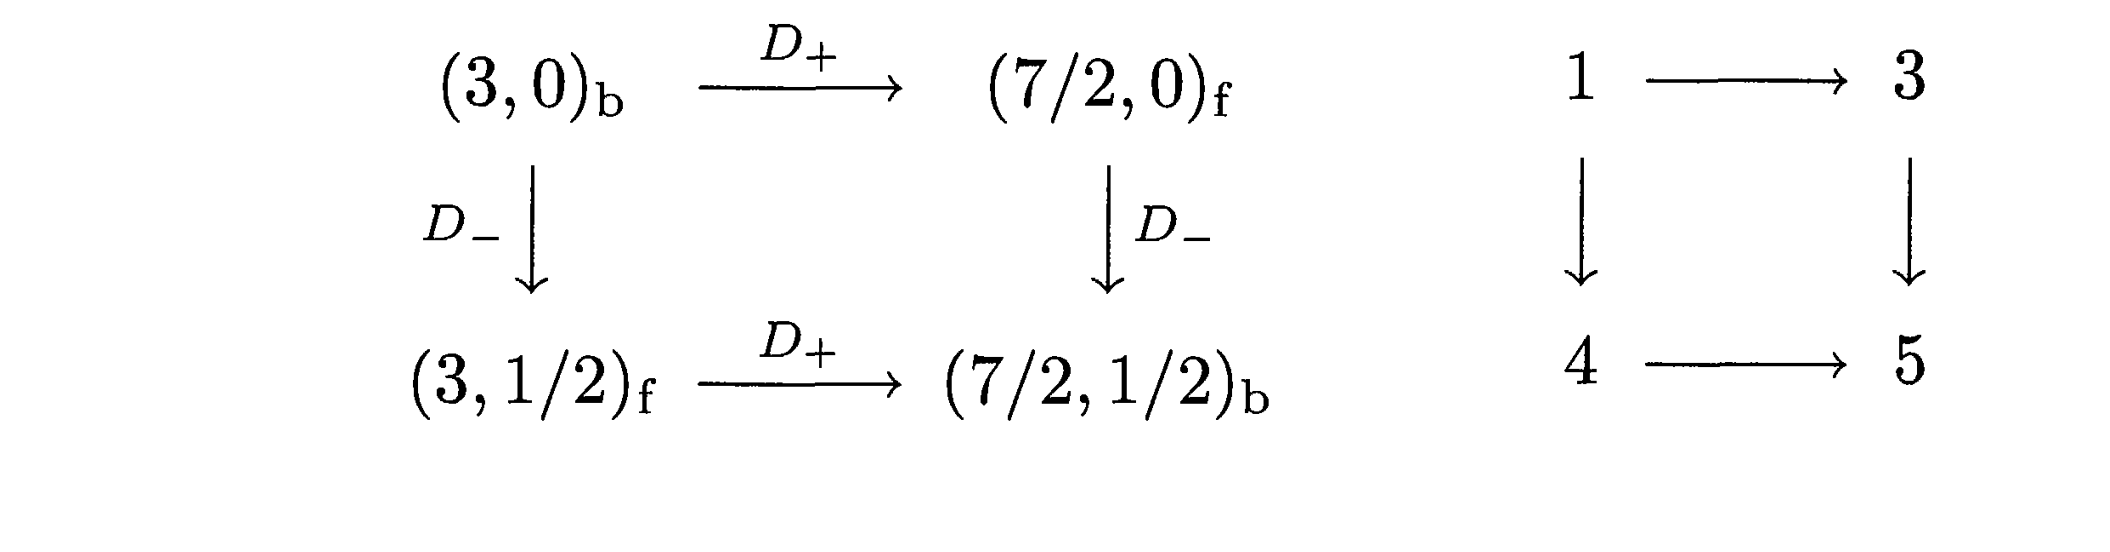
\includegraphics[width=0.86\textwidth]{figs/fig_p296_1.png}
  \caption{算符空间之间的 $D_\pm$ 作用与各空间维数。左：$(3,0)_{\mathrm b}\xrightarrow{D_+}(7/2,0)_{\mathrm f}$、$(3,1/2)_{\mathrm f}\xrightarrow{D_+}(7/2,1/2)_{\mathrm b}$，以及沿 $D_-$ 方向的竖直箭头；右：相应空间维数 $1\to3$、$4\to5$。（原文 Figure，未编号，p.296）}
  \label{fig:p296-1}
\end{figure}

% ===== 原文 p.297 =====
由量纲计数（与 §4.3 中相同）可知，我们可以取所需的 $\mathscr{X}_+$ 具有双分次 $(7/2,0)$，$\mathscr{X}_-$ 具有双分次 $(3,1/2)$。然后计算 $\mathcal{J}$ 的权重，从而得到相应守恒荷 $Q$ 的权重，结果是 $[K,Q]=3Q$，其中 $K$ 是 Lorentz 助推（Lorentz boost）。所以 $Q$ 不与 Poincaré 对易，这正是我们所要的。

\subsection*{问题 5 的解答}

（a）这个模型有两个玻色场：一个映射 $\phi\colon\mathbb{R}^2\to\mathbb{R}^{n+1}$，以及一个「Lagrange 乘子」$\sigma\colon\mathbb{R}^2\to\mathbb{R}$。作用量为
\[
\mathcal{L}=\frac{1}{2\lambda}|d\phi|^2-\frac{i\sigma}{2}(|\phi|^2-1).
\]
容易算出经典运动方程
\[
\begin{aligned}
|\phi|^2&=1\\
\frac{\Delta}{\lambda}\phi&=i\sigma\phi .
\end{aligned}
\]
我们的 Laplacian「$\Delta$」是非负的。第一个方程说明 $\phi$ 映入 $n$ 维球面 $S^n$，第二个说明 $\phi$ 的 Laplacian 垂直于 $S^n$。这意味着 $\phi$ 是到 $S^n$ 的调和映射（harmonic map）。我们把 $\sigma$ 用 $\phi$ 表示为
\begin{equation}
  \sigma=\frac{1}{i\lambda}(\Delta\phi,\phi).
  \tag{5.1}
  \label{eq:sol5-1}
\end{equation}
差一个全导数，$\sigma=\frac{1}{i\lambda}|d\phi|^2$。

（b）按照方程 (5.1)，$\sigma$ 场的量纲为 2，因为 $\phi$ 是二维中的标量场、量纲为 0。我们预期两点函数在位置空间中的行为是
\[
\langle\sigma(x)\sigma(0)\rangle\sim\frac{1}{|x|^4}\qquad\text{当 }x\to0,
\]
等价地，在动量空间中的行为是
\begin{equation}
  \langle\sigma(q)\sigma(-q)\rangle\sim q^2\qquad\text{当 }q\to\infty,
  \tag{5.2}
  \label{eq:sol5-2}
\end{equation}
其中可能有源于反常维数（anomalous dimension）的对数修正。我们可以先把 $\sigma$ 场积掉，从而得到到 $S^n$ 的 $\sigma$ 模型；由于这个理论是渐近自由的（asymptotically free），$|d\phi|^2$ 的两点函数确实呈现 (5.2) 的行为（相差对数修正）。这里我们反过来做：先积掉 $\phi$，计算 $\sigma$ 的有效作用量，至少在大 $n$ 极限下。

有效作用量的计算出现在本讲义 §4.2：
\begin{equation}
  \Gamma(\tilde\sigma)=\frac{n}{2}\left\{\operatorname{Tr}\ln(\Delta-i\tilde\sigma\tilde\lambda)+i\tilde\sigma\right\}.
  \tag{5.3}
  \label{eq:sol5-3}
\end{equation}
其中 $\tilde\sigma=\sigma/n$，$\tilde\lambda=\lambda n$。我们知道应当围绕值 $-i\tilde\sigma_0\tilde\lambda=M^2$（$M^2$ 为正常数）展开。$\tilde\sigma$ 传播子（propagator）是作用量 (5.3) 的

% ===== 原文 p.298 =====
二阶导数，我们在常数 $\tilde\sigma_0=iM^2/\tilde\lambda$ 处取值：
\begin{align}
\left.\frac{\delta^2\Gamma}{\delta\tilde\sigma^2}\right|_{\tilde\sigma_0}
&=\frac{n\tilde\lambda^2}{2}\operatorname{Tr}\left((\Delta+M^2)^{-1}\delta\tilde\sigma\,(\Delta+M^2)^{-1}\delta\tilde\sigma\right)\notag\\
&=\frac{n\tilde\lambda^2}{2}\int dx\,dy\,G(x,y)\,\delta\tilde\sigma(y)\,G(y,x)\,\delta\tilde\sigma(x)\tag{5.4}\label{eq:sol5-4}\\
&=\frac{n\tilde\lambda^2}{2}\int dx\,dy\,G(x,y)^2\,\delta\tilde\sigma(x)\,\delta\tilde\sigma(y),\notag
\end{align}
其中 $G$ 是 Green 函数 $(\Delta+M^2)^{-1}$ 的核。于是 $\tilde\sigma$ 的逆传播子的核为 $\frac{n\tilde\lambda^2}{2}G(x,y)^2$。在动量空间中，平方变为卷积（convolution），于是 $\tilde\sigma$ 逆传播子的核为
\begin{align}
K(q,-q)&=\frac{n\tilde\lambda^2}{2}\int\frac{d^2p}{(2\pi)^2}\,\frac{1}{p^2+M^2}\,\frac{1}{(q-p)^2+M^2}\notag\\
&=\frac{n\tilde\lambda^2}{8\pi^2}\int_0^1 d\alpha\int d^2p\,\frac{1}{[p^2+M^2+\alpha(1-\alpha)q^2]^2}\notag\\
&=\frac{n\tilde\lambda^2}{8\pi}\int_0^1\frac{d\alpha}{M^2+\alpha(1-\alpha)q^2}\tag{5.5}\label{eq:sol5-5}\\
&=\frac{n\tilde\lambda^2}{4\pi}\,\frac{\ln\left(\dfrac{\sqrt{1+4M^2/q^2}+1}{\sqrt{1+4M^2/q^2}-1}\right)}{q^2\sqrt{1+4M^2/q^2}}\notag\\
&\sim\frac{n\tilde\lambda^2}{2\pi}\,\frac{\ln(q^2/M^2)}{q^2}\qquad\text{当 }q\to\infty .\notag
\end{align}

% [Tutor Note: 由第二行到第三行用了二维的 Feynman 参数化与积分 $\int\frac{d^2p}{(2\pi)^2}\frac{1}{(p^2+\Delta)^2}=\frac{1}{4\pi\Delta}$（四维是 $\frac{1}{16\pi^2\Delta}$，最易混错）；把它与 $\frac{n\tilde\lambda^2}{8\pi^2}$ 中的 $(2\pi)^{-2}$ 合并，得到的正是 $\frac{n\tilde\lambda^2}{8\pi}\cdot\frac{1}{\Delta}$，系数中的 $8\pi$（而非 $8\pi^2$）是二维的标志。由第三行到第四行是标准的 $\int_0^1\frac{d\alpha}{M^2+\alpha(1-\alpha)q^2}=\frac{2}{q\sqrt{q^2+4M^2}}\ln\frac{\sqrt{q^2+4M^2}+\sqrt{q^2}}{\sqrt{q^2+4M^2}-\sqrt{q^2}}$；大 $q$ 时它趋于 $\frac{2}{q^2}\ln\frac{q^2}{M^2}$，恰好把 $\frac{1}{4\pi}$ 变成末行的 $\frac{1}{2\pi}$，故末行系数是自洽的。]

于是 $\tilde\sigma$ 传播子的行为是
\[
\langle\tilde\sigma(q)\tilde\sigma(-q)\rangle\sim\frac{2\pi}{n\tilde\lambda^2}\,\frac{q^2}{\ln(q^2/M^2)}\qquad\text{当 }q\to\infty .
\]
由 $\tilde\sigma=\sigma/n$，我们最终得到
\begin{equation}
  \langle\sigma(q)\sigma(-q)\rangle\sim\frac{2\pi n}{\tilde\lambda^2}\,\frac{q^2}{\ln(q^2/M^2)}\qquad\text{当 }q\to\infty .
  \tag{5.6}
  \label{eq:sol5-6}
\end{equation}

注意：对 $n$ 的依赖本可由 (5.1) 预言，因为 $(\Delta\phi,\phi)$ 的两点函数是单个标量场两点函数的 $n+1$ 倍。大 $q$ 的行为正如 (5.2) 所预言，只是被一个对数所修正。

注意：逆传播子 (5.5) 可以用图来计算。把我们的 $\phi$ 积掉所得的有效作用量，由带外 $\sigma$ 线、内 $\phi$ 线的图来计算。当然，我们应当围绕 $\sigma=iM^2/\lambda$ 展开。对二次项只有一个图，如图所示；图中实线代表 $\phi$，点线代表 $\sigma$。注意由于 $\sigma$ 的平移，$\phi$ 的传播子是有质量的。这个图正是由 (5.5) 计算的。

\begin{figure}[htbp]
  \centering
  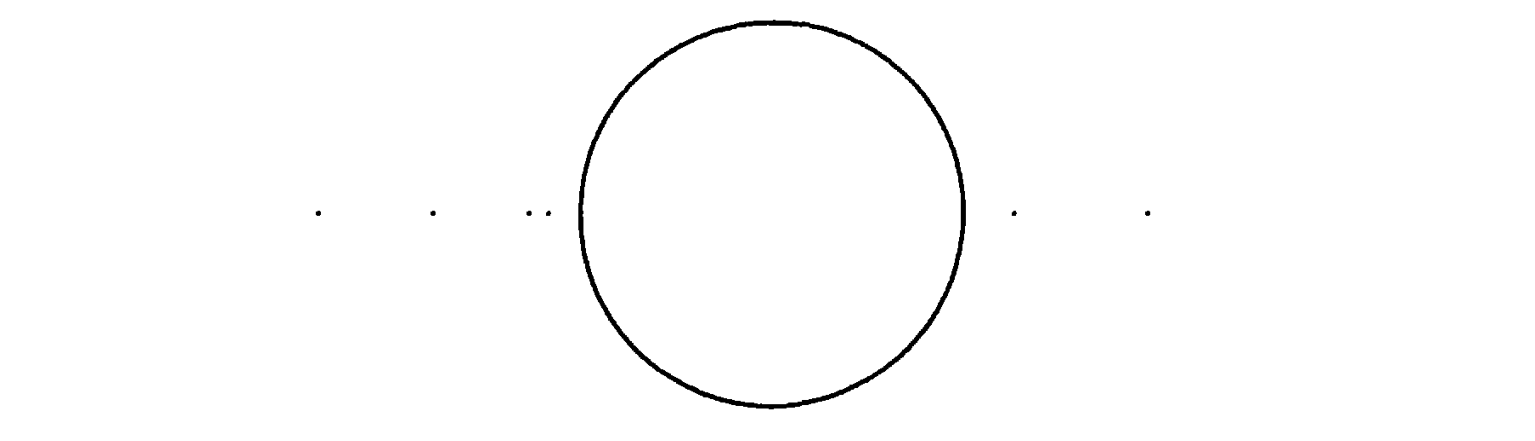
\includegraphics[width=0.55\textwidth]{figs/fig_p298_1.png}
  \caption{二次项的唯一一个图：实线圆环为内 $\phi$ 线，两侧点线为外 $\sigma$ 线。（原文 Figure，未编号，p.298）}
  \label{fig:p298-1}
\end{figure}

% ===== 原文 p.299 =====
\subsection*{问题 10 的解答}

我们沿用 [I-Supersolutions] 的记号与约定。

二维中的手征超场（chiral superfield）$\Phi$ 具有分量场 $\phi,\psi_\pm,\bar\psi_\pm$。以 $K$ 记无穷小旋转生成元，以 $J_-$ 与 $J_+$ 记 R 对称性的无穷小生成元（在第 14 讲中称为 $J_L$ 与 $J_R$）。我们所考虑的拓扑扭曲（topological twist）取 $K-\frac12J_-+\frac12J_+$ 作为欧氏旋转的新的无穷小生成元。下面的表格给出各分量场在这些无穷小对称性下的权重：

\begin{center}
\begin{tabular}{c|cccc}
\hline
分量场 & $K$ & $J_-$ & $J_+$ & $K-\frac12J_-+\frac12J_+$\\
\hline\hline
$\phi$ & $0$ & $0$ & $0$ & $0$\\
$\psi_+$ & $1/2$ & $0$ & $1$ & $1$\\
$\bar\psi_+$ & $1/2$ & $0$ & $-1$ & $0$\\
$\psi_-$ & $-1/2$ & $1$ & $0$ & $-1$\\
$\bar\psi_-$ & $-1/2$ & $-1$ & $0$ & $0$\\
\hline
\end{tabular}
\end{center}

% [Tutor Note: 用最后一列可自检扭曲是否正确：$\bar\psi_+$ 与 $\bar\psi_-$ 的新权重都是 0，故 $\bar\chi=\bar\psi_++\bar\psi_-$ 是 $\Sigma$ 上的标量；$\psi_+$ 权重 $1$、$\psi_-$ 权重 $-1$，分别给出 $(1,0)$ 与 $(0,1)$ 形式——这正是「把超 Riemann 面映到 Kähler 流形」所要求的。易错处有二：其一，$K$ 的归一化（此处旋转生成元在 $\psi_\pm$ 上取 $\pm1/2$，若改用 $\pm1$ 的约定，整列都要乘 2）；其二，$J_\pm$ 的符号，$\bar\psi_+$ 的 $J_+=-1$ 与 $\psi_+$ 的 $J_+=+1$ 差一个符号，若抄错，$\bar\psi_+$ 的新权重会变成 1，$\bar\chi$ 就不再是标量。]

超对称 $\bar Q_++\bar Q_-$ 与新的旋转生成元对易，因此它是扭曲后理论的超对称。

考虑扭曲理论中一个把超 Riemann 面映入 Kähler 流形（Kähler manifold）$X$ 的手征超场。表格的最后一列表明各分量场在底流形 $\Sigma$ 上如何变换。于是 $\phi$ 是从底流形 $\Sigma$ 到 $X$ 的映射，奇场 $\bar\psi_\pm$ 是 $\Sigma$ 上的标量、取值于反全纯切丛 $\phi^*T_{0,1}X$，而奇场 $\psi_+$（相应地 $\psi_-$）是 $\Sigma$ 上的 $(1,0)$ 形式（相应地 $(0,1)$ 形式）、取值于全纯切丛 $\phi^*T_{1,0}X$。定义新的奇场 $\bar\chi$ 与 $\bar\chi'$ 会比较方便：
\begin{equation}
  \begin{aligned}
    \bar\chi&=\bar\psi_++\bar\psi_-,\\
    \bar\chi'&=\bar\psi_+-\bar\psi_- .
  \end{aligned}
  \tag{10.1}
  \label{eq:sol10-1}
\end{equation}

现在我们取目标空间 $X=\mathbb{C}^n$ 这一特殊情形。如本讲义 §14.3.1 所解释的，我们把拓扑期望值的计算归结为对场的最低模（lowest modes）的积分。当 $\Sigma$ 的亏格（genus）为 0 时，不存在全纯的 $(1,0)$ 形式（也不存在反全纯的 $(0,1)$ 形式），因此我们可以消去 $\psi_\pm$。其余场 $\phi,\bar\chi,\bar\chi'$ 都化为常数。对这些常数场，我们用量纲约化 [I-Supersolutions, §5.1] 中最后那些方程的办法来计算超对称变换律。对 $\delta=\bar\eta(\bar Q_++\bar Q_-)$，我们得到
\[
\begin{aligned}
\delta\bar\phi&=-\sqrt2\,\bar\eta\,\bar\chi\\
\delta\bar\chi&=0\\
\delta\bar\chi'&=2\sqrt2\,\bar\eta\,\overline{\operatorname{grad}W(\phi)}.
\end{aligned}
\]

% [Tutor Note: 这三行都是 $\bar Q_++\bar Q_-$ 的变分，作用对象是带上横线的场，故第一行左端是 $\delta\bar\phi$；第三行右端「$\operatorname{grad}W(\phi)$」上方的横线表示对 $\phi$ 取共轭（即 $\partial\bar W/\partial\bar\phi$），不是排印污迹。自洽性检验：$\delta^2\bar\chi'=2\sqrt2\,\bar\eta\,\overline{\operatorname{Hess}W}\cdot\delta\bar\phi\propto\bar\eta^2=0$，故在常数场上 $\delta^2=0$，这正是拓扑（BRST 型）对称性所要求的；若忽略第一行的横线、把 $\phi$ 与 $\bar\phi$ 混为一谈，就会得出 $\delta^2\bar\chi'\neq0$ 的错误结论。]
这些场的 Lagrange 量，由量纲约化 [I-Supersolutions, §5.3] 中的一般 Lagrange 量、限制到常数场、再 Wick 转动到欧氏号差而得到：
\[
L=\|\operatorname{grad}W(\phi)\|^2-\frac12\operatorname{Hess}\overline{W}(\phi)(\bar\chi',\bar\chi).
\]

% 原文 pp.300–306（印刷 pp.1418–1424）
% 本文件承接 sol_p1.tex。p.300 起为「习题 10 的解答」的后半段，该页中部转入「习题 11 的解答」。

% ===== 原文 p.300 =====
\subsection{习题 10 的解答（续）}

如问题陈述中所说明，我们只取单个可观测量，它是 $P(\phi)$ 的一个多项式。于是前述讨论表明，它的单点函数（one-point function）$E$ 归结为对 $\mathbb{C}^n$ 以及对奇变量（odd variables）的一个有限维积分：
\begin{equation}
  \tag{10.2}
  \label{eq:sol10-2}
  E=\int P(\phi)\,e^{-\|\operatorname{grad}W(\phi)\|^2+\frac12\operatorname{Hess}\overline{W}(\phi)(\bar\chi',\bar\chi)}
  \frac{d^n\bar\phi\,d^n\phi}{(2\pi i)^n}\,d^n\bar\chi\,d^n\bar\chi'.
\end{equation}

为使此式有意义，我们注意到 $d^n\bar\phi\,d^n\bar\chi$ 具有典范的意义，因为 $d^n\bar\phi$ 是 $\operatorname{Det}T^*_{0,1}$ 的一个截面，而 $d^n\bar\chi$ 是 $\operatorname{Det}T_{0,1}$ 的一个截面。然而 $d^n\phi$ 是 $\operatorname{Det}T^*_{1,0}$ 的截面，$d^n\bar\chi'$ 是 $\operatorname{Det}T_{0,1}\cong\operatorname{Det}T^*_{1,0}$ 的截面，其中最后一个同构用到了 $\mathbb{C}^n$ 上标准的 Hermite 度量。因此我们必须选定一个元素
\[
  \omega=d^n\phi\,d^n\bar\chi'\in(\operatorname{Det}T^*_{1,0})^{\otimes2},
\]
才能把积分 (10.2) 定义为一个数。

% [Tutor Note: (10.2) 的指数里 $\frac12\operatorname{Hess}\overline W(\phi)(\bar\chi',\bar\chi)$ 的两个 Grassmann 变量都带横杠、且其中一个带撇，撇不是求导而是区分两个独立变量的记号；若误把 $\bar\chi'$ 当作 $\bar\chi$ 的某种导数，就会把该二次型写成 $\operatorname{Hess}W$ 而非 $\operatorname{Hess}\overline W$，从而丢掉整个反全纯因子。另注意测度 $\frac{d^n\bar\phi\,d^n\phi}{(2\pi i)^n}$ 与 $d^n\bar\chi\,d^n\bar\chi'$ 的配对是 Berezin 积分已经做掉的部分，故下面「费米子积分很容易做出」只是把两个 Grassmann 变量积掉，留下 $\epsilon^{-n}\det\operatorname{Hess}\overline W$。]

% [Tutor Note: 末式 $E=\sum_{\text{crit pts}}\frac{P(\phi_i)}{\det\operatorname{Hess}W(\phi_i)}$ 并不是靠「Gauss 近似」凑出来的巧合，而是 Atiyah–Bott 不动点公式（等价于 Poincaré–Hopf 定理）在 $W$ 的梯度流上的特例：$\delta$-恰当的作用量使积分局域化，分母的行列式正是临界点的 Morse 指标符号。作者用「Gaussian 近似」的说法跳过了这一步，读者若想补足，可查 Atiyah–Bott, \emph{Topology} 6 (1967) 或 Witten 的《Supersymmetry and Morse theory》。]

如 §14.3.1 中所解释，拓扑关联函数（topological correlation function）与 lagrangian 中的绝大多数参数无关。的确，在这个有限维模型中 $L$ 是恰当的（exact），由 (10.1) 可以算出：
\[
  \bar\eta L=\delta\Bigl\{\frac{1}{2\sqrt2}\bigl\langle\bar\chi',\operatorname{grad}W(\phi)\bigr\rangle\Bigr\}.
\]

这意味着在 (10.2) 中我们可以在指数上插入一个常数 $1/\epsilon$ 而不改变答案。（无论如何，总有 $\Sigma$ 的体积这个因子进入作用量，从而进入 (10.2) 中被积函数的指数。）

% [Tutor Note: 「可以插入 $1/\epsilon$」的依据是 $L=\delta(\cdots)$ 的 $\delta$-恰当性：由于 $\delta$ 是作用量所对应的 BRST 型算子，$\int e^{-S-\frac1\epsilon\delta\Psi}=\int e^{-S}$（差一个拓扑不变量），取 $\Psi=\frac{1}{2\sqrt2}\langle\bar\chi',\operatorname{grad}W\rangle$ 便得到指数上的 $\frac1\epsilon\|\operatorname{grad}W\|^2$。注意这里的 $\bar\eta$ 与 $\delta$ 是同一套记号中的两个算子（$\bar\eta$ 为「上同调」方向、$\delta$ 为其伴随），不可与 (11.x) 中的超对称变分 $\delta$ 混为一谈。]

费米子积分很容易做出，于是我们把 $E$ 的计算归结为 $\mathbb{C}^n$ 上一个普通的积分：
\[
  E=\int_{\mathbb{C}^n}P(\phi)\,\epsilon^{-n}\det\operatorname{Hess}\overline{W}(\phi)\,
  e^{-\frac1\epsilon\|\operatorname{grad}W(\phi)\|^2}\frac{d^n\bar\phi\,d^n\phi}{(2\pi i)^n}.
\]

注意我们用 $\bar\omega$ 把 $\det\operatorname{Hess}\overline{W}(\phi)$ 解释为一个数。在 $\epsilon\to0$ 的极限下，剩下的积分局域化到 $W$ 的临界点集上。为简单起见，设 $W$ 具有孤立的非退化临界点。在临界点附近我们用 Gauss 积分近似该积分，这给出分母上的 $\|\det\operatorname{Hess}W(\phi)\|^2$。它与被积函数中的反全纯部分相消，最终结果是
\[
  E=\sum_{\text{临界点 }\phi_i}\frac{P(\phi_i)}{\det\operatorname{Hess}W(\phi_i)}.
\]

\subsection{习题 11 的解答}

在着手路径积分之前，我们先回顾\footnote{% 原文脚注 1
关于此计算的至少一部分，参考文献是 S.~K. Donaldson, P.~Kronheimer, \emph{The Geometry of Four-Manifolds}, Oxford University Press, New York, 1990, p.~197.}一个关于某种万有曲率（universal curvature）的公式。设 $P\to\Sigma$ 是 Riemann 流形 $\Sigma$ 上的主 $G$-丛。以 $\mathcal{A}_P$ 记 $P$ 上联络构成的空间，$\mathcal{G}_P$ 记规范变换群。以下我们自由地在联络 $A$ 与它所决定的 $\bar\partial$ 算子之间来回切换

% 原句跨页：p.301 开头「(complex structure) it defines on associated bundles by its (1,0) part」是本句的插入语，译文见下页首行。

% ===== 原文 p.301 =====
（即它由其 $(1,0)$ 部分在相伴丛上定义的复结构）。现在，丛 $\mathcal{A}_P\times_P X\to\mathcal{A}_P\times X$ 上有一个万有联络（tautological connection）。要把它下降到商\footnote{% 原文脚注 2
此项讨论中我们忽略奇点（singularities）。}$\mathcal{P}\to(\mathcal{A}_P/\mathcal{G}_P)\times X$ 上，我们需要 $\mathcal{A}_P\to\mathcal{A}_P/\mathcal{G}_P$ 上的一个水平分布，这可以通过取轨道（orbits）的正交补而得到。现在限制到 $\mathcal{M}_P\times X$，其中 $\mathcal{M}_P$ 是平坦联络模去规范变换所得的模空间。我们进一步限制到不可约联络。$\mathcal{M}_P$ 在 $A$ 的等价类处的切向量是上同调群 $H^1_A(\mathfrak{g}^P)$ 的一个元素，它由 $\Sigma$ 上一个取值于伴随丛的 1-形式 $\alpha$ 代表。给定两个这样的 $\alpha_1,\alpha_2$，此联络在 $\mathcal{P}\to\mathcal{M}_P\times X$ 上沿 $\mathcal{M}_P$ 的切方向的曲率 $\omega_1$ 为
\[
  \omega_1(\alpha_1,\alpha_2)=2\Delta_A^{-1}\bigl\langle[\alpha_1\wedge\alpha_2]\bigr\rangle,
\]
其中 $\Delta_A=d_A^*d_A$ 是 $\Omega^0(\mathfrak{g}^P)$ 上的 Laplace 算子（laplacian），而记号 $\langle[\alpha_1\wedge\alpha_2]\rangle$ 的意思是：对 $\alpha_i=a_i\otimes\zeta_i\in\Omega^1\otimes\mathfrak{g}$，
\begin{equation}
  \tag{11.1}
  \label{eq:sol11-1}
  \bigl\langle[a_1\otimes\zeta_1,a_2\otimes\zeta_2]\bigr\rangle=\langle a_1,a_2\rangle[\zeta_1,\zeta_2].
\end{equation}

若 $\Sigma$ 是 Riemann 面，我们用 $\square_A:\Omega^0(\mathfrak{g}^P)\to\Omega^2(\mathfrak{g}^P)$（由 $\square_A=-d_A*d_A$ 定义）把 (11.1) 改写为
\begin{equation}
  \tag{11.2}
  \label{eq:sol11-2}
  \omega_1(\alpha_1,\alpha_2)=2\square_A^{-1}[\alpha_1\wedge*\alpha_2].
\end{equation}

% [Tutor Note: 这里最容易出错的是算子的「次数」。$\Delta_A=d_A^*d_A$ 作用在 $\Omega^0$ 上（作为算子是负定的），故 $\Delta_A^{-1}$ 把 0-形式送回 0-形式；而 (11.2) 中的 $\square_A$ 被定义成 $\Omega^0\to\Omega^2$，它把 0-形式送到 2-形式（即 $\square_A f=\Delta f$ 配上体积元），因此 $\square_A^{-1}$ 只能吃 2-形式。$[\alpha_1\wedge*\alpha_2]$ 恰好是 2-形式（$\alpha_i$ 为 1-形式、$*\alpha_2$ 为 1-形式），所以 (11.2) 的两边都是标量函数。若把 $\square_A^{-1}$ 误当作通常的 Laplace 逆算子（$\Omega^0\to\Omega^0$），就会为形式次数不匹配而困惑，也容易丢掉 (11.2) 相对 (11.1) 中 Hodge 星号带来的一个符号。]

（尽管我们并不使用这一事实，但请注意 $\omega_1$ 只依赖于 $\Sigma$ 的共形结构。）

现在固定 Hermite 向量空间 $W$ 上的一个酉表示 $\rho:G\to U(W)$，并令 $W^P\to\Sigma$ 为相伴的 Hermite 向量丛。平凡（无穷秩）丛 $\mathcal{A}_P\times\Omega^0(W^P)$ 在限制到平坦联络之后，于规范变换下下降为丛 $\mathcal{S}\to\mathcal{M}_P$。这个丛也可以描述为 $W^P\to\mathcal{M}_P\times X$ 的相对截面（relative sections）丛。$\mathcal{P}\to\mathcal{M}_P\times X$ 上的联络诱导 $\mathcal{S}\to\mathcal{M}_P$ 上的一个联络：给定 $\mathcal{M}_P$ 的一个切向量，我们把它平凡地提升到 $\mathcal{M}_P\times X$，并逐点地在 $W^P$ 中作用协变导数。这个联络保持 $\mathcal{S}\to\mathcal{M}_P$ 上的 $L^2$ 度量，后者由 $W^P\to\Sigma$ 上逐点的内积对 $\Sigma$ 上的 Riemann 测度积分而得到。该联络的曲率由逐点地作用 $\dot\rho(\omega)$ 给出。我们实际上关心的是取值于 $W$ 的 $(0,1)$-形式，它是固定的复线丛 $\Lambda^{0,1}$ 与 $W^P$ 张量积的截面空间。联络与曲率都看不见这个线丛，所以公式 (11.2) 保持不变。现在考虑 $\Lambda^{0,1}\otimes W^P$ 的相对调和截面（relative harmonic sections）构成的子丛。它是一个有限维子丛\footnote{% 原文脚注 3
我们把讨论限制在使 $H^0(W^P)$ 为零的那些复结构上。}
\begin{equation}
  \tag{11.3}
  \label{eq:sol11-3}
  H^1(W^P)\to\mathcal{M}_P
\end{equation}
它是 $\mathcal{S}\to\mathcal{M}_P$ 的子丛，而我们可以用 $L^2$ 度量把联络投影到它上面。这个投影联络的曲率于是等于 (11.2) 逐点作用于全纯截面的投影，再加上一个第二基本形式（second fundamental form）项。以 $\pi_A$ 记到 $\Omega^{0,1}(W^P)$ 中关于联络 $A$ 调和的形式上的投影。稍作计算可知该第二基本形式项为
\begin{equation}
  \tag{11.4}
  \label{eq:sol11-4}
  \begin{aligned}
    \omega_2(\alpha_1,\alpha_2)
    &=\pi_A\,\dot\rho_{\mathbb{C}}\bigl(\alpha_2^{(0,1)}\bigr)\Delta_A^{-1}*\dot\rho_{\mathbb{C}}\bigl(\alpha_1^{(1,0)}\bigr)\pi_A\\
    &\quad-\pi_A\,\dot\rho_{\mathbb{C}}\bigl(\alpha_1^{(0,1)}\bigr)\Delta_A^{-1}*\dot\rho_{\mathbb{C}}\bigl(\alpha_2^{(1,0)}\bigr)\pi_A.
  \end{aligned}
\end{equation}

% [Tutor Note: (11.4) 的反对称性完全依赖于第二项前面的那个负号；$\omega_2$ 是 2-形式，必须满足 $\omega_2(\alpha_1,\alpha_2)=-\omega_2(\alpha_2,\alpha_1)$，读者可用此检验是否抄错了指标 $1\leftrightarrow2$。另注意算子的次序不可交换：$\dot\rho_{\mathbb{C}}(\alpha^{(0,1)})$ 先把 $(0,1)$-形式乘成取值于 $W$ 的形式，再经 $\Delta_A^{-1}*$ 变回 $(0,1)$-形式（星号把两个 $(0,1)$ 因子的乘积变回 $(0,1)$ 型），最后 $\pi_A$ 投到调和部分；若把 $\Delta_A^{-1}$ 与 $\dot\rho$ 交换，结果会多出与曲率有关的项。]

% ===== 原文 p.302 =====
(11.3) 的曲率为下述和
\begin{equation}
  \tag{11.5}
  \label{eq:sol11-5}
  \pi_A\omega_1\pi_A+\omega_2.
\end{equation}

现在转向物理。扭曲手征超场（twisted chiral superfield）有分量场（component fields）\footnote{% 原文脚注 4
在 [I-Supersolutions, §9.2] 中我们用的是 $\lambda_\pm$，它们与这里所用的 [I-Supersolutions, §6.2] 的 $\lambda^\pm$ 由
\[
  \lambda^+=-\lambda_-,\qquad \lambda^-=\lambda_+
\]
相联系。}$\sigma,\lambda^\pm,\bar\lambda^\pm$，它们取值于伴随丛 $\mathfrak{g}^P$。此外 $P$ 上还有一个联络 $A$。与习题 10 中一样，手征超场有分量场 $\phi,\psi_\pm,\bar\psi_\pm$，它们是相伴 Hermite 丛 $V^P$（或其共轭 $\overline{V}^P$）的截面。这里所用的拓扑扭曲与习题 10 中的不同；它与超对称 $\overline{Q}_++Q_-$ 对易。我们总结于下表：

\begin{table}[htbp]
  \centering
  \caption{扭曲手征超场各分量场的量子数。（原文表格，p.302）}
  \label{tab:p302}
  \renewcommand{\arraystretch}{1.18}
  \begin{tabular}{|c|c|c|c|c|}
    \hline
    分量场 & $K$ & $J_-$ & $J_+$ & $K+\frac12J_-+\frac12J_+$\\
    \hline\hline
    $A$ & $1\oplus-1$ & $0$ & $0$ & $1\oplus-1$\\
    \hline
    $\sigma$ & $0$ & $1$ & $-1$ & $0$\\
    \hline
    $\bar\sigma$ & $0$ & $-1$ & $1$ & $0$\\
    \hline
    $\lambda^+$ & $-1/2$ & $0$ & $-1$ & $-1$\\
    \hline
    $\bar\lambda^+$ & $-1/2$ & $0$ & $1$ & $0$\\
    \hline
    $\lambda^-$ & $1/2$ & $-1$ & $0$ & $0$\\
    \hline
    $\bar\lambda^-$ & $1/2$ & $1$ & $0$ & $1$\\
    \hline
    $\phi$ & $0$ & $0$ & $0$ & $0$\\
    \hline
    $\bar\phi$ & $0$ & $0$ & $0$ & $0$\\
    \hline
    $\psi_+$ & $1/2$ & $0$ & $1$ & $1$\\
    \hline
    $\bar\psi_+$ & $1/2$ & $0$ & $-1$ & $0$\\
    \hline
    $\psi_-$ & $-1/2$ & $1$ & $0$ & $0$\\
    \hline
    $\bar\psi_-$ & $-1/2$ & $-1$ & $0$ & $-1$\\
    \hline
  \end{tabular}
\end{table}

这里 $K$ 是旋转的无穷小生成元，$J_\pm$ 是 R 对称性（R-symmetries）。在曲面 $\Sigma$ 上的扭曲理论中，我们把 $\sigma,\bar\sigma$ 解释为取值于伴随丛的复标量；$\lambda^-,\bar\lambda^+$ 为奇的伴随值复标量；$\bar\lambda^-$ 为 $\Sigma$ 上取值于复化伴随丛的 $(1,0)$-形式；$\lambda^+$ 为 $\Sigma$ 上取值于复化伴随丛的 $(0,1)$-形式；$\phi$ 为 $V^P$ 的截面；$\bar\psi_+$（相应地 $\psi_-$）为 $\overline{V}^P$（相应地 $V^P$）的奇截面；$\psi_+$ 为 $\Sigma$ 上取值于 $V^P$ 的 $(1,0)$-形式；$\bar\psi_-$ 为 $\Sigma$ 上取值于 $\overline{V}^P$ 的 $(0,1)$-形式。

% [Tutor Note: 脚注 4 的等式在印刷本上左右两边的符号是同一套 $\lambda^\pm$，因此字面上是自我指涉的（$\lambda^+=-\lambda^-$ 与 $\lambda^-=\lambda^+$ 不能用同一组符号同时成立）。其原意应是：左边为 [I-Supersolutions, §9.2] 的下标记号 $\lambda_\pm$，右边为本讲所用、即 [I-Supersolutions, §6.2] 的上标记号 $\lambda^\pm$，即 $\lambda_+=-\lambda^-$、$\lambda_-=\lambda^+$。这一处记号冲突在对照该丛书第 I 卷使用时必须留意，否则 (11.6)–(11.7) 中的 $\pm$ 会整体反号。]

差 $J_--J_+$ 与 $\overline{Q}_++Q_-$ 对易，而用这个对称性来检查下面的 lagrangian 与方程式是否平衡是很方便的。

lagrangian 由四维中一般的 $\mathcal{N}=1$ lagrangian 经维数约化（dimensional reduction）得到。有关的公式出现在 [I-Supersolutions, §6.2] 中「$\mathbb{F}=\mathbb{C}$」的情形下。我们取那里的 lagrangian，维数约化到两维，然后 Wick 转动到欧氏空间。设

% 原句「Let ρ̇_C: g_C → End(V) denote ...」自 p.302 末行起，主语与谓语在下页首行。

% [Tutor Note: [I-Supersolutions] 指本丛书第 I 卷（\emph{Quantum Fields and Strings} 第 1 册）所附超对称习题解答一章；本书正文中凡 [I-...]、[II-...] 皆为此类卷内互引，页码随版本而异，核对时以节号（此处 §6.2、§9.2、§9.3）为准。]

% ===== 原文 p.303 =====
$\dot\rho_{\mathbb{C}}:\mathfrak{g}_{\mathbb{C}}\to\operatorname{End}(V)$ 为 $G$ 在 $V$ 上作用的复化无穷小作用（complexified infinitesimal action）。我们得到（维数约化后的 Yang–Mills 作用量见 [I-Supersolutions, §9.3]）：
\begin{equation}
  \tag{11.6}
  \label{eq:sol11-6}
  L_e=\left\{\begin{aligned}
    &\tfrac12|F_A|^2+\langle d_A\bar\sigma,d_A\sigma\rangle+\langle d_A\bar\phi,d_A\phi\rangle
      +\langle\bar\lambda\not D_A\lambda\rangle+\langle\bar\psi\not D_A\psi\rangle\\
    &+\tfrac12\|[\sigma,\bar\sigma]\|^2+2\|\dot\rho_{\mathbb{C}}(\sigma)\phi\|^2+2|\mu(\phi)|^2\\
    &-\sqrt2\bigl(\langle\bar\lambda^-,[\bar\sigma,\lambda^+]\rangle
      +\langle\bar\lambda^+,[\sigma,\lambda^-]\rangle\bigr)\\
    &+\sqrt2\bigl(\langle\bar\psi_-,\dot\rho_{\mathbb{C}}(\sigma)\psi_+\rangle
      +\langle\bar\psi_+,\dot\rho_{\mathbb{C}}(\bar\sigma)\psi_-\rangle\bigr)\\
    &+\sqrt2\bigl(\langle\dot\rho_{\mathbb{C}}(\lambda^a)^*\phi^*,\psi_a\rangle
      -\langle\bar\psi_{\dot a},\dot\rho_{\mathbb{C}}(\bar\lambda^{\dot a})\phi\rangle\bigr)
  \end{aligned}\right\}|d^2x|.
\end{equation}

% [Tutor Note: 最后一行是全式最易抄错的地方：求和指标在第一个括号里写成上标 $a$（$\lambda^a$、$\psi_a$ 一上一下缩并），在第二个括号里却写成带点的 $\dot a$（$\bar\lambda^{\dot a}$、$\bar\psi_{\dot a}$）。点指标与无点指标分别对应 $\pm$ 两个分量，且二者只能成对缩并、不能互相替换；若把 $\bar\psi_{\dot a}$ 写成 $\bar\psi_a$，就会在费米子符号上出错。另注意 $(\dot\rho_{\mathbb{C}}(\lambda^a))^*$ 是对算子的 Hermite 共轭，作者把星号写在括号外，不要误读成对 $\lambda^a$ 取共轭。]

在第二行中，$\mu:V\to\mathfrak{g}^*$ 是 $G$ 在 $V$ 上作用的矩映射（moment map）。最后一行的求和是对 $\pm$ 求和。倒数第二项的记号在 [I-Supersolutions, §6.2] 中有解释；它其实就是最后一项的复共轭。第三、四行的项来自把四维中的费米子动能项作维数约化；第二行中的第二项来自把四维中的 $\langle d_A\bar\phi,d_A\phi\rangle$ 作维数约化。类似地，我们把各场的超对称变换律维数约化到两维，作 Wick 转动，并特殊化到扭曲理论的超对称 $\delta=\eta(\overline{Q}_++Q_-)$。所得方程为（纯规范理论的变换律见 [I-Supersolutions, §9.2]）：
\begin{equation}
  \tag{11.7}
  \label{eq:sol11-7}
  \begin{array}{r@{\qquad}l}
    (\delta A)_{1,0}=2\eta\bar\lambda^- & \delta\lambda^+=-2\sqrt2\,\eta\,\bar\partial_A\sigma\\[3pt]
    (\delta A)_{0,1}=2\eta\lambda^+ & \delta\bar\lambda^+=\eta i\bigl(\tilde f_A+2\tilde\mu(\phi)-i[\sigma,\bar\sigma]\bigr)\\[3pt]
    \delta\sigma=0 & \delta\lambda^-=-\eta i\bigl(\tilde f_A+2\tilde\mu(\phi)\bigr)+i[\sigma,\bar\sigma])\\[3pt]
    \delta\bar\sigma=-\sqrt2\,\eta\,(\lambda^-+\bar\lambda^+) & \delta\bar\lambda^-=2\sqrt2\,\eta\,\partial_A\sigma\\[3pt]
    \delta\phi=-\sqrt2\,\eta\,\psi_- & \delta\psi_+=-2\sqrt2\,\eta\,\partial_A\phi\\[3pt]
    \delta\bar\phi=-\sqrt2\,\eta\,\bar\psi_+ & \delta\bar\psi_+=2\eta\,\dot\rho_{\mathbb{C}}(\bar\sigma)\bar\phi\\[3pt]
    & \delta\psi_-=2\eta\,\dot\rho_{\mathbb{C}}(\sigma)\phi\\[3pt]
    & \delta\bar\psi_-=-2\sqrt2\,\eta\,\bar\partial_A\bar\phi
  \end{array}
\end{equation}

% [Tutor Note: 原文 $\delta\lambda^-$ 一行右端的圆括号不配对：印刷为 $-\eta i(\tilde f_A+2\tilde\mu(\phi))+i[\sigma,\bar\sigma])$，末尾多出一个右括号。译文照原样保留以便对照。按上一行 $\delta\bar\lambda^+$ 的结构推断，原意应为 $-\eta i\bigl(\tilde f_A+2\tilde\mu(\phi)+i[\sigma,\bar\sigma]\bigr)$（即方括号项也在括号内），但这属于推测，未擅改。]

这里 $\tilde\mu:V\to\mathfrak{g}$ 是由矩映射 $\mu:V\to\mathfrak{g}^*$ 借助 $\mathfrak{g}$ 上的度量构造出来的。我们用到了标准算子
\[
  \partial=\frac12\Bigl(\frac{\partial}{\partial\tau}-i\frac{\partial}{\partial x}\Bigr)
\]
及其共轭（在 $\mathbb{R}^2$ 上）。$A$ 的曲率是\footnote{% 原文脚注 5
在 [I-Supersolutions, §9.2] 中我们把 Minkowski 空间 $M^2$ 中规范场 $A$ 的曲率写成
\[
  F_A=-f_A\,dt\wedge dx
\]
其中 $t,x$ 是 $M^2$ 上的标准坐标。在联络与曲率中都作代换 $\tau=it$，我们得到 (11.8)，其中 $\tilde f_A=if_A$。}
\begin{equation}
  \tag{11.8}
  \label{eq:sol11-8}
  F_A=\tilde f_A\,d\tau\wedge dx.
\end{equation}

% [Tutor Note: 这个 $\partial=\frac12(\partial_\tau-i\partial_x)$ 的约定决定了 $(1,0)$ 与 $(0,1)$ 的归属：它等于复坐标 $z=\tau+ix$ 下的 $\partial_z$，因此 $\partial$ 把标量变成 $(1,0)$-形式、$\bar\partial$ 变成 $(0,1)$-形式。用 (11.7) 校验：$\delta\psi_+=-2\sqrt2\eta\,\partial_A\phi$ 而 $\psi_+$ 是 $(1,0)$-形式（表中 $K=1/2$），$\delta\lambda^+=-2\sqrt2\eta\,\bar\partial_A\sigma$ 而 $\lambda^+$ 是 $(0,1)$-形式（$K=-1/2$），两者自洽。若改用常见的 $z=x+i\tau$，则 $\partial$ 与 $\bar\partial$ 互换，$K$ 的分配会整体反号，这是核对本页时最常见的错误来源。]

% ===== 原文 p.304 =====
在扭曲之后，这些公式在 Riemann 面 $\Sigma$ 上继续成立。

按照 §14.3.1 中所述的不动点思想，拓扑关联函数的泛函积分局域化到在超对称下不变的玻色子位形上。因此玻色子方程由令 $\delta(\text{费米子})$ 变换律的右端为零而得到。在我们的问题中，由 (11.7) 得到
\begin{equation}
  \tag{11.9}
  \label{eq:sol11-9}
  \begin{array}{c}
    \tilde f_A=-2\tilde\mu(\phi)\\[3pt]
    \partial_A\sigma=\bar\partial_A\sigma=0\\[3pt]
    \bar\partial_A\bar\phi=0\\[3pt]
    [\sigma,\bar\sigma]=0\\[3pt]
    \dot\rho_{\mathbb{C}}(\sigma)\phi=0.
  \end{array}
\end{equation}

现在，酉群 $U(V)$ 在 $V$ 上作用的矩映射由下述公式给出
\begin{equation}
  \tag{11.10}
  \label{eq:sol11-10}
  \mu(\phi)(T)=-\frac{i}{2}\langle\bar\phi,T\phi\rangle,\qquad \phi\in V,\quad T\in\mathfrak{u}(V).
\end{equation}

我们借助 $\dot\rho:\mathfrak{g}\to\mathfrak{u}(V)$ 作拉回，得到 $G$ 在 $V$ 上作用的矩映射。若 $\mathfrak{g}$ 没有可交换的因子，则这是唯一可能。此时，若表示是不可约的，则 $\mu(\phi)=0$ 的唯一解是 $\phi=0$。于是泛函积分被约化到 (11.3) 的零截面。我们把自己限制在这一情形。我们还进一步假设丛的选取使得 $H^0_A(W^P)=0$，其中
\[
  W=\overline{V},
\]
或者更确切地说，我们限制到使这一点成立的那些复结构。于是由 (11.9) 中第三个方程可得 $\bar\phi=0$。第一个方程随即蕴含 $A$ 是平坦的，因为由 (11.10) 矩映射为零。我们假设 $A$ 不可约，从而第二个方程蕴含 $\sigma=0$。其余方程不带来任何新的东西。总结起来，玻色不动点的方程为：
\[
  A\ \text{平坦}
\]
\[
  \phi=\sigma=0.
\]

现在来看费米子。按照 §14.3 中铺陈的一般原理，我们归结为对费米子的最低模积分。§14.4 中已说明，若 $A$ 不可约（我们正作此假设），则可以令复标量为零
\[
  \lambda^-=\bar\lambda^+=0.
\]
此外，在 $H^0_A(W^P)=0$ 的假设下我们有
\[
  \psi_-=\bar\psi_+=0.
\]
非零的费米子零模是
\[
  \chi:=\psi_+,\qquad \bar\chi:=\bar\psi_-,\qquad \lambda^+,\qquad \bar\lambda^-,
\]

% 原句以逗号结束于 p.304 末，其谓语「restricted to be harmonic 1-forms」在 p.305 首行。

% ===== 原文 p.305 =====
它们被限制为调和 1-形式。

我们现在可以计算一个拓扑可观测量的期望值了。如问题陈述中所述，并且从 (11.7) 显而易见，这些可观测量是 $\sigma$ 及其后代（descendents）的多项式，正如 §14.4 中讨论的纯规范理论那样。按拓扑场论的一般原理（§14.3.1），路径积分约化到由满足 (11.9) 的玻色位形与费米子零模所构成的超流形的一个邻域。玻色子 $A$ 与零模 $\lambda^+,\bar\lambda^-$ 一起构成 $\Pi T\mathcal{M}_P$，而如 §14.4 中所解释，$\Pi T\mathcal{M}_P$ 上的积分等价于 $\mathcal{M}_P$ 上一个微分形式的积分。对 $\chi,\bar\chi$ 的零模的积分是向量空间 $\Pi H^1_A(W^P)$ 上的费米子积分。我们把这些场的非零模、以及其余各场——$\phi,\bar\phi,\sigma,\bar\sigma,A,\bar\lambda^+,\lambda^-,\bar\psi_+,\psi_-$——在作用量的二次近似下沿到 $\Pi(T\mathcal{M}_P\times H^1_A(W^P))$ 的法丛积掉，从而化归为这些有限维积分。该积分是 Gauss 型的，因此可以显式做出。然后我们再计算 $\Pi H^1_A(W^P)$ 上的积分，从而化为 $\mathcal{M}_P$ 上一个微分形式的积分。只有在最后一步，拓扑可观测量才进入，因此我们的计算结果将是一个微分形式，它乘在对应于该可观测量的形式上。我们将认出这个形式就是 (11.3) 的 Euler 形式（Euler form）。

% [Tutor Note: $\Pi$ 是「奇（parity-reversed）化」的记号：$\Pi T\mathcal{M}_P$ 指把 $\mathcal{M}_P$ 的切丛的纤维改成奇（Grassmann）变量所得的超丛，故玻色子 $A$ 与费米子零模 $\lambda^+,\bar\lambda^-$ 可以同处一个超流形上；$\Pi H^1_A(W^P)$ 同理。$\Pi$ 不是投影算子，也不表示圆周，抄录时极易与 $\prod$ 或 $\pi$ 混淆。]

首先，我们做标量场 $\phi,\bar\phi,\sigma,\bar\sigma$ 上的 Gauss 积分。在 lagrangian (11.6) 中我们略去第二行的势能项，因为它们在这些标量场中是四次（quartic）的。作用量中剩下的是一个无穷维积分，它类似于下面 $\mathbb{C}^N$ 上的积分：
\[
  \iint_{\mathbb{C}^N}\frac{d\overline{\Phi}\,d\Phi}{(2\pi i)^N}
  e^{-(\overline{\Phi}Q\Phi+\overline{\Phi}L+\overline{L}\Phi)}
  =(\det Q)^{-1}e^{\overline{L}Q^{-1}L}.
\]

这里 $Q$ 是 Hermite 算子，故 $\overline{\Phi}Q\Phi$ 是实二次型；$L$ 是复线性算子，故 $\overline{\Phi}L+\overline{L}\Phi$ 是实线性型。在我们的问题中 $\Phi=\binom{\phi}{\sigma}$，并且
\[
  Q=\square_A
\]
\[
  L=\sqrt2\begin{pmatrix}
    \dot\rho_{\mathbb{C}}(\lambda^a)\psi_a\\[2pt]
    [\lambda^+,\bar\lambda^-]+B(\bar\chi,\chi)
  \end{pmatrix}
\]
其中双线性形式 $B$ 满足
\begin{equation}
  \tag{11.11}
  \label{eq:sol11-11}
  \langle\bar\chi,\dot\rho_{\mathbb{C}}(\bar\sigma)\chi\rangle
  =\langle\bar\sigma,B(\bar\chi,\chi)\rangle.
\end{equation}

注意 $L$ 在费米子中是二次的，所以 $\overline{L}Q^{-1}L$ 在费米子中是四次的。对 $A$ 的非零模也有类似的玻色积分。$A$ 的含费米子的相互作用项——$\langle\bar\lambda\not D_A\lambda\rangle$ 与 $\langle\bar\psi\not D_A\psi\rangle$——把 $\bar\lambda^\pm$ 与 $\lambda^\pm$ 配对、把 $\bar\psi_\pm$ 与 $\psi_\pm$ 配对。当我们限制到零模时，这样的配对为零，因此尽管这个积分给出有效作用量中费米子四次的项，那些项却不起作用。当然，$A$ 的非零模上的积分还给出一个逆行列式。

其次，我们对所有费米子的非零模积分。费米子的有效 lagrangian 形如
\[
  \langle\bar\lambda\not D_A\lambda\rangle+\langle\bar\psi\not D_A\psi\rangle
  +\overline{\mathcal{L}}\,\mathcal{Q}^{-1}\mathcal{L}
\]

% ===== 原文 p.306 =====
其中 $\mathcal{Q},\mathcal{L}$ 包含 $Q,L$ 以及对应于 $A$ 的相应形式。在 Gauss 近似下我们略去四次项 $\overline{\mathcal{L}}\mathcal{Q}^{-1}\mathcal{L}$，只剩下一个简单的 Gauss 积分。它给出分子上的行列式，恰好与玻色行列式相消。

我们剩下的是对零模 $\chi,\bar\chi,\lambda^+,\bar\lambda^-$ 的费米子积分，以及对 $\mathcal{M}_P$ 的一个玻色积分。如前所述，我们只做 $\chi,\bar\chi$ 上的积分，以约化到 $\Pi T\mathcal{M}_P$ 上的积分。有效 lagrangian 现在只涉及势项 $\overline{\mathcal{L}}\mathcal{Q}^{-1}\mathcal{L}$，而限制到零模上它是
\[
  -2\bigl\langle\dot\rho_{\mathbb{C}}(\bar\lambda^-)^*\bar\chi,\square_A^{-1}\dot\rho_{\mathbb{C}}(\lambda^+)\chi\bigr\rangle
  +2\bigl\langle B(\chi,\bar\chi),\square_A^{-1}[\lambda^+,\bar\lambda^-]\bigr\rangle.
\]

根据 (11.11)，我们可以把第二项改写为
\[
  -2\bigl\langle\bar\chi,\dot\rho_{\mathbb{C}}\bigl(\square_A^{-1}[\lambda^+,\bar\lambda^-]\bigr)\chi\bigr\rangle.
\]

（这是原作用量 (11.6) 中的一项，只是把 $\sigma$ 代换成了其运动方程的解 $\square_A\sigma=-\sqrt2[\lambda^+,\bar\lambda^-]$。）于是我们所拥有的积分是
\begin{equation}
  \tag{11.12}
  \label{eq:sol11-12}
  \iint_{H^1_A(W^P)}\frac{D\bar\chi\,D\chi}{(2\pi i)^m}
  e^{\int_\Sigma\langle\bar\chi,\omega\chi\rangle}
  =\frac{\det(\omega)}{(2\pi i)^m},
\end{equation}
其中 $m=\dim H^1(W)$，并且
\[
  -\omega=2\dot\rho_{\mathbb{C}}\bigl(\square_A^{-1}[\lambda^+,\bar\lambda^-]\bigr)
  +2\dot\rho_{\mathbb{C}}(\bar\lambda^-)\square_A^{-1}\dot\rho_{\mathbb{C}}(\lambda^+).
\]

在 (11.12) 中 $\omega$ 作用在 $\chi$ 上，而 $\chi$ 是 $(1,0)$ 型的。为与 (11.5) 比较，我们需要写出伴随算子 $\omega^*$，它作用在 $(0,1)$ 型的 $\bar\chi$ 上。回忆 $\dot\rho$ 在实向量上是斜 Hermite 的（skew-Hermitian），可见 $\omega$ 的伴随是
\[
  \omega^*=2\dot\rho_{\mathbb{C}}\bigl(\square_A^{-1}[\lambda^+,\bar\lambda^-]\bigr)
  -2\dot\rho_{\mathbb{C}}(\lambda^+)\square_A^{-1}\dot\rho_{\mathbb{C}}(\bar\lambda^-).
\]

由 (11.5)，对应于 $\omega^*$ 的微分形式是 $H^1(V^P)\to\mathcal{M}_P$ 的曲率的两倍，故 $-\omega^*$ 是共轭丛 $H^1(W^P)\to\mathcal{M}_P$ 的曲率形式的两倍。因此，(11.12) 等于 $H^1(W^P)\to\mathcal{M}_P$ 的曲率的行列式的 $(i/\pi)^m$ 倍，而这个行列式是该「障碍丛」（obstruction bundle）的 Euler 形式的 $2^m$ 倍\footnote{% 原文脚注 6
勤勉的读者也许能从更细致的计算中发现这个因子并不出现。想来这可以通过仔细处理 $\chi,\bar\chi$ 上积分的归一化而得到解决。}。

% [Tutor Note: 这里的 $2^m$ 是作者本人也承认的未定因子（见脚注 6）：Grassmann 测度 $D\bar\chi D\chi$ 的归一化与 Euler 形式的 $2^m$（Pfaffian）约定不匹配，故引用 (11.12) 时只应取「相差一个只依赖 $m$ 的常数」这层意思，不要把 $2^m$ 当作可验证的系数。另注意 (11.12) 左边 $\omega$ 吃的是 $(1,0)$ 型的 $\chi$，而要对接 (11.5) 必须先取伴随 $\omega^*$ 换成作用在 $(0,1)$ 型 $\bar\chi$ 上的算子；这一步隐含用 Hermite 度量把 $H^1$ 与其共轭等同，跳过伴随就直接比较会误用 $\dot\rho$ 的斜 Hermite 性。]


% ---------------------------- 附录 A：术语表 ----------------------------
\clearpage
\markboth{附录 A：术语表}{附录 A：术语表}
\section*{附录 A\quad 术语表（英—中对照）}
\addcontentsline{toc}{section}{附录 A：术语表}
% 术语表（英—中对照）
\begin{longtable}{@{}p{0.215\linewidth}p{0.28\linewidth}p{0.215\linewidth}p{0.28\linewidth}@{}}
\toprule
英文 & 中文 & 英文 & 中文 \\
\midrule
\endfirsthead
\toprule
英文 & 中文 & 英文 & 中文 \\
\midrule
\endhead
\bottomrule
\endfoot
quantum field theory & 量子场论 & gauge theory & 规范场论 \\
gauge field & 规范场 & gauge transformation & 规范变换 \\
connection & 联络 & curvature & 曲率 \\
holonomy & 和乐 & Wilson loop & Wilson 圈 \\
't Hooft loop & 't Hooft 圈 & confinement & 禁闭 \\
asymptotic freedom & 渐近自由 & renormalization group & 重整化群 \\
beta function & $\beta$ 函数 & anomalous dimension & 反常维数 \\
anomaly & 反常 & anomaly cancellation & 反常抵消 \\
path integral & 路径积分 & partition function & 配分函数 \\
correlation function & 关联函数 & Green's function & Green 函数 \\
vacuum expectation value & 真空期望值 & order parameter & 序参量 \\
spontaneous symmetry breaking & 自发对称性破缺 & Goldstone boson & Goldstone 玻色子 \\
Higgs mechanism & Higgs 机制 & effective action & 有效作用量 \\
effective potential & 有效势 & loop correction & 圈修正 \\
tadpole & 蝌蚪图 & one-particle irreducible & 单粒子不可约 \\
operator product expansion & 算符乘积展开（OPE） & conformal field theory & 共形场论（CFT） \\
instanton & 瞬子 & soliton & 孤子 \\
kink & 扭结（kink） & monopole & 磁单极子 \\
vortex & 涡旋 & topological charge & 拓扑荷 \\
Bogomolny bound & Bogomolny 界 & BPS state & BPS 态 \\
moduli space & 模空间 & moduli space of vacua & 真空模空间 \\
supersymmetry & 超对称 & superfield & 超场 \\
chiral superfield & 手征超场 & twisted chiral superfield & 扭曲手征超场 \\
superpotential & 超势 & Kähler potential & Kähler 势 \\
R-symmetry & $R$ 对称性 & central charge & 中心荷 \\
topological twist & 拓扑扭曲 & topological field theory & 拓扑场论 \\
Donaldson theory & Donaldson 理论 & Seiberg--Witten theory & Seiberg--Witten 理论 \\
$u$-plane & $u$ 平面 & Seiberg--Witten curve & Seiberg--Witten 曲线 \\
sigma model & $\sigma$ 模型 & Grassmannian & Grassmann 流形 \\
Wess--Zumino--Witten model & Wess--Zumino--Witten 模型 & Wess--Zumino term & Wess--Zumino 项 \\
BRST quantization & BRST 量子化 & BRST cohomology & BRST 上同调 \\
ghost & 鬼场 & antighost & 反鬼场 \\
Faddeev--Popov determinant & Faddeev--Popov 行列式 & gauge fixing & 规范固定 \\
Grassmann variable & Grassmann 变量 & Berezin integral & Berezin 积分 \\
Bose--Fermi correspondence & Bose--Fermi 对应 & bosonization & 玻色化 \\
large $N$ limit & 大 $N$ 极限 & 't Hooft limit & 't Hooft 极限 \\
planar diagram & 平面图 & double-line notation & 双线记号 \\
Landau--Ginzburg model & Landau--Ginzburg 模型 & minimal model & 极小模型 \\
quantum cohomology & 量子上同调 & mirror symmetry & 镜像对称 \\
Calabi--Yau manifold & Calabi--Yau 流形 & Fano variety & Fano 簇 \\
intersection theory & 相交理论 & characteristic class & 示性类 \\
Chern class & Chern 类 & Euler characteristic & Euler 特征数 \\
index theorem & 指标定理 & Dirac operator & Dirac 算符 \\
Hodge theory & Hodge 理论 & complex structure & 复结构 \\
Kähler manifold & Kähler 流形 & hermitian metric & Hermite 度量 \\
theta angle & $\theta$ 角 & Chern--Simons term & Chern--Simons 项 \\
theta term & $\theta$ 项 & instanton number & 瞬子数 \\
S-matrix & $S$ 矩阵 & LSZ reduction & LSZ 约化 \\
Feynman diagram & Feynman 图 & scattering amplitude & 散射振幅 \\
cross section & 截面 & spectral representation & 谱表示 \\
gauge group & 规范群 & representation & 表示 \\
irreducible representation & 不可约表示 & character & 特征标 \\
adjoint bundle & 伴随丛 & associated bundle & 伴随丛（associated bundle） \\
principal bundle & 主丛 & section & 截面 \\
Dirac monopole & Dirac 磁单极子 & 't Hooft--Polyakov monopole & 't Hooft--Polyakov 磁单极子 \\
\end{longtable}


% ---------------------------- 附录 B：文献代号 ----------------------------
\clearpage
\markboth{附录 B：原书文献代号}{附录 B：原书文献代号}
\section*{附录 B\quad 原书文献代号与参考文献说明}
\addcontentsline{toc}{section}{附录 B：原书文献代号说明}

原书（AMS 版 \emph{Quantum Fields and Strings: A Course for Mathematicians}，两卷本）
以方括号代号互引，正文中出现的主要代号含义如下：

\begin{center}
\begin{tabular}{@{}ll@{}}
\toprule
代号 & 所指 \\
\midrule
\texttt{[I-Perturbative QFT]} & 第 I 卷中关于微扰量子场论的讲义 \\
\texttt{[I-Homework]} & 第 I 卷所附超对称习题集 \\
\texttt{[II-CFT]} & 第 II 卷中关于共形场论的讲义 \\
\texttt{[I-Supersolutions]} & 第 I 卷所附超对称习题解答 \\
\texttt{[II-...]} & 第 II 卷相应讲义，依此类推 \\
\bottomrule
\end{tabular}
\end{center}

其余文献引用（如 Witten 关于 Donaldson 理论、Seiberg--Witten 理论、镜像对称的论文，
Atiyah--Singer 指标定理，Coleman 关于二维对称性破缺的定理等）保留原文作者的姓与年份，
可在正文批注给出的线索下查核原始文献。译注本不另编参考文献表，以免与原文编号冲突。

\vspace{1.5em}
\noindent\rule{0.4\linewidth}{0.4pt}\\[0.4em]
{\small 译注本完成于二〇二六年十月。译文与批注中若有疏漏，文责在译者。}

\end{document}
